\documentclass[a4paper,11pt]{report}
%%%%%%%%%%%%%%%%%%%%%%%%%%%%%%%%%%%%%%%%%%%%%%%%%%%%%%%%%%%%%%%%%%%%%%%%%%%%%%%%%%%%%%%%%%%%%%%%%%%

\usepackage[utf8]{inputenc}
\usepackage{graphicx}
\usepackage{pdflscape}
\usepackage[cm]{fullpage}
\usepackage{upgreek}
\usepackage{bm}
\usepackage{mdframed}
\usepackage{amsmath}
\usepackage{amsfonts}
\usepackage{xcolor} 
\usepackage{dsfont}
\usepackage{gensymb} %\degree
\usepackage{listings}
\usepackage{stmaryrd}
\usepackage{multicol}
\usepackage{lipsum}
\usepackage{verbatim}
\usepackage[colorinlistoftodos,prependcaption,textsize=tiny]{todonotes}

\usepackage{siunitx} 
\DeclareSIUnit\year{yr}
\DeclareSIUnit\day{day}

\renewcommand{\chaptername}{Stone}

\usepackage{tikz}
\usetikzlibrary{arrows, arrows.meta}

\usepackage{hyperref}
\hypersetup{
colorlinks,
citecolor=black,
filecolor=black,
linkcolor=violet,
urlcolor=black}

\lstset{ 
  language=Python,
  backgroundcolor=\color{white},   % choose the background color; you must add \usepackage{color} or \usepackage{xcolor}; should come as last argument
  basicstyle=\footnotesize,        % the size of the fonts that are used for the code
  breakatwhitespace=false,         % sets if automatic breaks should only happen at whitespace
  breaklines=true,                 % sets automatic line breaking
  captionpos=b,                    % sets the caption-position to bottom
  frame=single,                    % adds a frame around the code
  keepspaces=true,                 % keeps spaces in text, useful for keeping indentation of code (possibly needs columns=flexible)
  keywordstyle=\color{blue},       % keyword style
}


\newcommand{\inpython}{\fbox{\textbf{\large \color{teal} P}}}
\newcommand{\injulia}{\fbox{\textbf{\large \color{purple} J}}}
\newcommand{\infortran}{\fbox{\textbf{\large \color{orange} F}}}

\newcommand{\aspect}{{\textsc{Aspect~}{}}}
\newcommand{\elefant}{{\textsc{Elefant~}{}}}
\newcommand{\citcoms}{{\textsc{CitcomS~}{}}}
\newcommand{\citcomsve}{{\textsc{CitcomSVE~}{}}}
\newcommand{\fantom}{{\textsc{Fantom~}{}}}
\newcommand{\sulec}{{\textsc{Sulec~}{}}}
\newcommand{\sopale}{{\textsc{Sopale~}{}}}
\newcommand{\douar}{{\textsc{Douar~}{}}}
\newcommand{\ghost}{{\textsc{Ghost~}{}}}
\newcommand{\fluidity}{{\textsc{Fluidity~}{}}}
\newcommand{\sepran}{{\textsc{Sepran~}{}}}
\newcommand{\stone}{{\color{teal} {\textsc{stone~}}}}
\newcommand{\etal}{{\it et al.~}}
\newcommand{\nn}{\nonumber}
\newcommand{\A}{{\mathbb{A}}}
\newcommand{\K}{{\mathbb{K}}}
\newcommand{\J}{{\mathbb{J}}}
\newcommand{\G}{{\mathbb{G}}}
\newcommand{\Z}{{\mathbb{Z}}}
\newcommand{\C}{{\mathbb{C}}}
\newcommand{\W}{{\mathbb{W}}}
\newcommand{\R}{{\mathbb{R}}}
\newcommand{\M}{{\mathbb{M}}}
\newcommand{\N}{{\mathbb{N}}}
\newcommand{\LLL}{{\mathbb{L}}}
\newcommand{\SSS}{{\mathbb{S}}}
\newcommand{\QQQ}{{\color{violet}\cal Q}}
\newcommand{\FFF}{{\color{violet}\cal F}}
\newcommand{\III}{{\color{PineGreen}\cal I}}
\newcommand{\KKK}{{\color{RoyalBlue}\cal K}}
\newcommand{\HH}{{\mathbb{H}}}
\newcommand{\Literature}{\includegraphics[height=4mm]{images/lit} {\sffamily Relevant Literature}}
\newcommand{\captionfont}{\tiny}
\newcommand{\pythonfile}{\color{blue} \sffamily }
\newcommand{\shellscriptfile}{\color{purple} \sffamily }
\newcommand{\asciifile}{\color{olive} \sffamily }
\newcommand{\OK}{{\bf OK}}
\newcommand{\filenamefont }{\sl }
\newcommand{\foldernamefont }{\it }
\newcommand{\codefont}{\bfseries\ttfamily}
\newcommand{\Ranb}{{\mathsf{Ra}}}
\newcommand{\Rbnb}{{\mathsf{Rb}}}
\newcommand{\Renb}{{\mathsf{Re}}}
\newcommand{\Nunb}{{\mathsf{Nu}}}
\newcommand{\Prnb}{{\mathsf{Pr}}}
\newcommand{\Penb}{{\mathsf{Pe}}}
\newcommand{\Dinb}{{\mathsf{Di}}}
\newcommand{\Mnb}{{\mathsf{M}}}
\newcommand{\python}{\color{darkgray} \sffamily }
\newcommand{\bN}{{\mathcal{N}}}
\newcommand{\qx}{\underset{\tiny x}{q}}
\newcommand{\qy}{\underset{\tiny y}{q}}
\newcommand{\nx}{\underset{\tiny x}{n}}
\newcommand{\ny}{\underset{\tiny y}{n}}
\newcommand{\qhx}{\underset{\tiny x}{q_h}}
\newcommand{\qhy}{\underset{\tiny y}{q_h}}
\newcommand{\qix}{\underset{\tiny x}{q_i}}
\newcommand{\qiy}{\underset{\tiny y}{q_i}}
\newcommand{\Tx}{\underset{\tiny x}{T}}
\newcommand{\Ty}{\underset{\tiny y}{T}}
\newcommand{\blueqx}{  {\color{blue} \underset{\tiny x}{q}  }  }
\newcommand{\blueqy}{  {\color{blue} \underset{\tiny y}{q}  }  }
\newcommand{\blueT}{  {\color{blue} T}  }
\newcommand{\brownT}{  {\color{brown} T}  }
\newcommand{\brownqx}{  {\color{brown} \underset{\tiny x}{q}  }  }
\newcommand{\brownqy}{  {\color{brown} \underset{\tiny y}{q}  }  }
\newcommand\norm[1]{\left\lVert#1\right\rVert}

\newcommand{\QonePzero}{${Q}_1\times P_0$}
\newcommand{\QtwoQone}{${Q}_2\times Q_1$}
\newcommand{\QthreeQtwo}{${Q}_3\times Q_2$}
\newcommand{\QfourQthree}{${Q}_4\times Q_3$}
\newcommand{\QtwoPmone}{${Q}_2\times P_{-1}$}

\definecolor{carrotorange}{rgb}{0.93, 0.57, 0.13}
\definecolor{chestnut}{rgb}{0.8, 0.36, 0.36}

\newcommand{\nineteensixty}{{\color{chestnut}\bf 1960}}
\newcommand{\nineteensixtyone}{{\color{chestnut}\bf 1961}}
\newcommand{\nineteensixtytwo}{{\color{chestnut}\bf 1962}}
\newcommand{\nineteensixtythree}{{\color{chestnut}\bf 1963}}
\newcommand{\nineteensixtyfour}{{\color{chestnut}\bf 1964}}
\newcommand{\nineteensixtyfive}{{\color{chestnut}\bf 1965}}
\newcommand{\nineteensixtysix}{{\color{chestnut}\bf 1966}}
\newcommand{\nineteensixtyseven}{{\color{chestnut}\bf 1967}}
\newcommand{\nineteensixtyeight}{{\color{chestnut}\bf 1968}}
\newcommand{\nineteensixtynine}{{\color{chestnut}\bf 1969}}

\newcommand{\nineteenseventy}{{\color{carrotorange}\bf 1970}}
\newcommand{\nineteenseventyone}{{\color{carrotorange}\bf 1971}}
\newcommand{\nineteenseventytwo}{{\color{carrotorange}\bf 1972}}
\newcommand{\nineteenseventythree}{{\color{carrotorange}\bf 1973}}
\newcommand{\nineteenseventyfour}{{\color{carrotorange}\bf 1974}}
\newcommand{\nineteenseventyfive}{{\color{carrotorange}\bf 1975}}
\newcommand{\nineteenseventysix}{{\color{carrotorange}\bf 1976}}
\newcommand{\nineteenseventyseven}{{\color{carrotorange}\bf 1977}}
\newcommand{\nineteenseventyeight}{{\color{carrotorange}\bf 1978}}
\newcommand{\nineteenseventynine}{{\color{carrotorange}\bf 1979}}

\newcommand{\nineteeneighty}{{\color{violet}\bf 1980}}
\newcommand{\nineteeneightyone}{{\color{violet}\bf 1981}}
\newcommand{\nineteeneightytwo}{{\color{violet}\bf 1982}}
\newcommand{\nineteeneightythree}{{\color{violet}\bf 1983}}
\newcommand{\nineteeneightyfour}{{\color{violet}\bf 1984}}
\newcommand{\nineteeneightyfive}{{\color{violet}\bf 1985}}
\newcommand{\nineteeneightysix}{{\color{violet}\bf 1986}}
\newcommand{\nineteeneightyseven}{{\color{violet}\bf 1987}}
\newcommand{\nineteeneightyeight}{{\color{violet}\bf 1988}}
\newcommand{\nineteeneightynine}{{\color{violet}\bf 1989}}

\newcommand{\nineteenninety}{{\color{red}\bf 1990}}
\newcommand{\nineteenninetyone}{{\color{red}\bf 1991}}
\newcommand{\nineteenninetytwo}{{\color{red}\bf 1992}}
\newcommand{\nineteenninetythree}{{\color{red}\bf 1993}}
\newcommand{\nineteenninetyfour}{{\color{red}\bf 1994}}
\newcommand{\nineteenninetyfive}{{\color{red}\bf 1995}}
\newcommand{\nineteenninetysix}{{\color{red}\bf 1996}}
\newcommand{\nineteenninetyseven}{{\color{red}\bf 1997}}
\newcommand{\nineteenninetyeight}{{\color{red}\bf 1998}}
\newcommand{\nineteenninetynine}{{\color{red}\bf 1999}}
\newcommand{\twothousand}{{\color{teal}\bf 2000}}
\newcommand{\twothousandone}{{\color{teal}\bf 2001}}
\newcommand{\twothousandtwo}{{\color{teal}\bf 2002}}
\newcommand{\twothousandthree}{{\color{teal}\bf 2003}}
\newcommand{\twothousandfour}{{\color{teal}\bf 2004}}
\newcommand{\twothousandfive}{{\color{teal}\bf 2005}}
\newcommand{\twothousandsix}{{\color{teal}\bf 2006}}
\newcommand{\twothousandseven}{{\color{teal}\bf 2007}}
\newcommand{\twothousandeight}{{\color{teal}\bf 2008}}
\newcommand{\twothousandnine}{{\color{teal}\bf 2009}}
\newcommand{\twothousandten}{{\color{blue}\bf 2010}}
\newcommand{\twothousandeleven}{{\color{blue}\bf 2011}}
\newcommand{\twothousandtwelve}{{\color{blue}\bf 2012}}
\newcommand{\twothousandthirteen}{{\color{blue}\bf 2013}}
\newcommand{\twothousandfourteen}{{\color{blue}\bf  2014}}
\newcommand{\twothousandfifteen}{{\color{blue}\bf  2015}}
\newcommand{\twothousandsixteen}{{\color{blue}\bf 2016}}
\newcommand{\twothousandseventeen}{{\color{blue}\bf 2017}}
\newcommand{\twothousandeighteen}{{\color{blue}\bf 2018}}
\newcommand{\twothousandnineteen}{{\color{blue}\bf 2019}}
\newcommand{\twothousandtwenty}{{\color{purple}\bf 2020}}
\newcommand{\twothousandtwentyone}{{\color{purple}\bf 2021}}
\newcommand{\twothousandtwentytwo}{{\color{purple}\bf 2022}}
\newcommand{\twothousandtwentythree}{{\color{purple}\bf 2023}}
\newcommand{\twothousandtwentyfour}{{\color{purple}\bf 2024}}
\newcommand{\twothousandtwentyfive}{{\color{purple}\bf 2025}}

\newcommand\todoin[2][]{\todo[inline, #1]{
\begin{minipage}{\textwidth-3pt}#2\end{minipage}}}


\usepackage{xr}
\externaldocument[MMM-]{manual}

%%%%%%%%%%%%%%%%%%%%%%%%%%%%%%%%%%%%%%%%%%%%%%%%%%%%%%%%%%%

\usepackage{amsthm}
\newtheorem*{remark}{Remark}
\newtheorem{problem}{problem:}
\newtheorem{problem-bonus}{problem*}

%%%%%%%%%%%%%%%%%%%%%%%%%%%%%%%%%%%%%%%%%%%%%%%%%%%%%%%%%%%
%Bibliography stuff
%%%%%%%%%%%%%%%%%%%%%%%%%%%%%%%%%%%%%%%%%%%%%%%%%%%%%%%%%%%
\usepackage[maxnames=6]{biblatex}
\addbibresource{biblio_geosciences.bib}


%%%%%%%%%%%%%%%%%%%%%%%%%%%%%%%%%%%%%%%%%%%%%%%%%%%%%%%%%%%%%%%%%%%%%%%%%%%%%%%%%%%%%%%%%%%%%%%%%%%

\author{C. Thieulot}
\title{All the stones}

%%%%%%%%%%%%%%%%%%%%%%%%%%%%%%%%%%%%%%%%%%%%%%%%%%%%%%%%%%%

\usepackage{multind}
\makeindex{general}
\makeindex{contributors}
\makeindex{topics}

%%%%%%%%%%%%%%%%%%%%%%%%%%%%%%%%%%%%%%%%%%%%%%%%%%%%%%%%%%%%%%%%%%%%%%%%%%%%%%%%%%%%%%%%%%%%%%%%%%%
\begin{document}
\thispagestyle{empty}
\includegraphics[width=0.9\linewidth]{images/frontpage/frontpage.png}

\maketitle
\tableofcontents

%%%%%%%%%%%%%%%%%%%%%%%%%%%%%%%%%%%%%%%%%%%%%%%%%%%%%%%%%%%%%%%%%%%%%%%%%%%%%%%%%%%%%%%%%%%%%%%%%%%
\chapter*{Naming convention for every stone and elefant }

These have evolved in the first two years so that the early stones may not 
follow these conventions (yet).

\begin{tabular}{p{2.5cm}p{14cm}}
\hline
Variable & meaning \\
\hline
\hline
{\tt mV}    & number $m_\upnu$ of velocity nodes in the element \\
{\tt mP}    & number $m_p$ of pressure nodes in the element \\
{\tt mT}    & number $m_T$ of temperature nodes in the element \\
{\tt ndofV} & number of velocity degrees of freedom per velocity node \\
{\tt ndofP} & number of pressure degrees of freedom per pressure node \\
{\tt NV}    & total number of velocity nodes \\
{\tt NfemV} & total number of velocity degrees of freedom \\
{\tt NfemP} & total number of pressure degrees of freedom \\
{\tt Nfem}  & total number of degrees of freedom \\
{\tt nelx,nely,nelz} & number of elements in each direction \\
{\tt nel}   & total number of elements \\
{\tt nqel}  & number of quadrature points per element \\
{\tt xq,yq,zq} & coordinates of a quadrature point \\
{\tt uq,vq,wq} & velocity at a quadrature point \\
{\tt pq}   & pressure at a quadrature point \\
{\tt etaq} & viscosity value at a quadrature point \\
{\tt rhoq} & density value at a quadrature point \\
{\tt dt}   & time step $\delta t$\\ 
{\tt gx,gy,gz} & components of the gravity vector \\
{\tt jcob} & determinant of the Jacobian matrix \\
\hline
\end{tabular}

\vspace{.5cm}

\begin{tabular}{p{3.5cm}p{12.5cm}}
\hline
Array & meaning \\
\hline
\hline
{\tt iconV} & connectivity array for velocity nodes \\
{\tt iconP} & connectivity array for pressure nodes \\
{\tt qcoords\_r} & contains the $r$ coordinates of the {\tt nel} quadrature points \\
{\tt qcoords\_s} & contains the $s$ coordinates of the {\tt nel} quadrature points \\
{\tt qcoords\_t} & contains the $t$ coordinates of the {\tt nel} quadrature points \\
{\tt qweights} & contains the weights associated to the {\tt nel} quadrature points \\
{\tt xV,yV,zV} & coordinates of the {\tt NV} velocity nodes \\
{\tt xP,yP,zP} & coordinates of the {\tt NP} pressure nodes \\
{\tt bc\_fix} & boolean array of size {\tt NfemV}. Is true if a boundary condition
                is specify at a dof \\
{\tt bc\_val} & value of the boundary condition at a given dof \\
{\tt u,v,w} & velocity components \\ 
{\tt p} & pressure \\ 
{\tt q} & pressure projected onto the velocity nodes\\
{\tt NNNV} & velocity basis functions values at a quadrature point \\
{\tt dNNNVdr} & velocity basis functions derivatives values at a quadrature point \\
{\tt dNNNVds} & velocity basis functions derivatives values at a quadrature point \\
{\tt dNNNVdt} & velocity basis functions derivatives values at a quadrature point \\
{\tt NNNP} & pressure basis functions values at a quadrature point \\
{\tt b\_mat} & elemental gradient matrix ${\bm B}$ \\
{\tt K\_el}  & elemental stiffness matrix $\K_{el}$ \\
{\tt G\_el}  & elemental gradient matrix $\G_{el}$ \\
{\tt N\_mat}  & elemental ${\bm N}$ matrix \\
{\tt a\_mat}  & fully assembled Stokes matrix \\
{\tt A\_sparse} & Stokes matrix in {\tt lil\_matrix} format \\
{\tt exx,eyy,exy,...} & components of the strain rate tensor (elemental or nodal array)\\
{\tt tauxx,tauyy,tauxy,...} & components of the deviatoric stress tensor (elemental or nodal array)\\
{\tt jcb} & 2x2 or 3x3 Jacobian matrix \\
{\tt jcbi} & inverse of the Jacobian matrix \\
{\tt rhs} & right hand side vector \\
{\tt sol} & solution vector returned by the solver\\
\hline
\end{tabular}

\vspace{.5cm}

\begin{tabular}{p{2cm}p{14cm}}
\hline
Function & meaning \\
\hline
{\tt NNV}    & function which returns the value of all velocity basis functions 
               ${\cal N}_i^\upnu$ at a given location\\
{\tt dNNVdr} & function which returns the value of all velocity basis functions 
               ${\cal N}_i^\upnu$ derivative with respect to $r$ at a given location\\
{\tt dNNVds} & function which returns the value of all velocity basis functions 
               ${\cal N}_i^\upnu$ derivative with respect to $s$ at a given location\\
{\tt dNNVdt} & function which returns the value of all velocity basis functions 
               ${\cal N}_i^\upnu$ derivative with respect to $t$ at a given location\\
{\tt NNP}    & function which returns the value of all pressure basis functions 
               ${\cal N}_i^P$ at a given location\\
{\tt bx} & \\
{\tt by} & \\
{\tt bz} & \\
\hline
\end{tabular}



\chapter*{Stone 00: mesh generation in 1D, 2D, 3D \label{f00}} %%%%%%%%%%%%%%%%%%%%%%%%%%%%%%%%%%%% 00
\begin{flushright} {\tiny {\color{gray} python\_codes/fieldstone\_00/text.tex}} \end{flushright}


%--------------------------------------------
\subsection*{The node layout}

Let us start in one dimension. We wish to generate a 
set of $N$ discrete and equidistant $x$ coordinates 
between $0$ and $L_x$:

\begin{center}
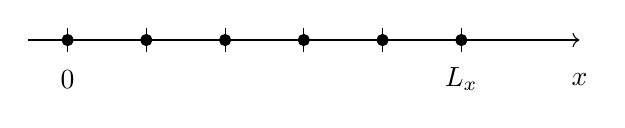
\begin{tikzpicture}
%\draw[fill=gray!23,gray!23](0,0) rectangle (8,2);
%\draw[step=0.5cm,gray,very thin] (0,0) grid (8,2); %background grid
\draw [->] (0.5,1) -- (7.5,1);
\draw[-] (1,0.85)--(1,1.15);
\draw[-] (2,0.85)--(2,1.15);
\draw[-] (3,0.85)--(3,1.15);
\draw[-] (4,0.85)--(4,1.15);
\draw[-] (5,0.85)--(5,1.15);
\draw[-] (6,0.85)--(6,1.15);
\node[] at (1,0.5) {$0$};
\node[] at (6,0.5) {$L_x$};
\node[] at (7.5,0.5) {$x$};
\draw[black,fill=black] (1,1)   circle (2pt);
\draw[black,fill=black] (2,1)   circle (2pt);
\draw[black,fill=black] (3,1)   circle (2pt);
\draw[black,fill=black] (4,1)   circle (2pt);
\draw[black,fill=black] (5,1)   circle (2pt);
\draw[black,fill=black] (6,1)   circle (2pt);
\end{tikzpicture}
\end{center}

\noindent
The distance between two consecutive coordinates is 
\[
h = \frac{L_x}{N-1}
\]
This simply translates as follows in Python:
\begin{lstlisting}
N=10
Lx=1
h=Lx/(N-1)
for i in range(0,N):
    print(i*h)
\end{lstlisting}

Since $i$ ranges from 0 to $N-1$ (because ... python!) the generated values go from 0 to $L_x$. 
Obviously I am doing this because I later wish to reuse these coordinates 
so I also wish to store them in an array.
I therefore need to declare and array of size $N$ which will 
contain all $N$ coordinates:
\begin{lstlisting}
import numpy as np
N=10
Lx=1
h=Lx/(N-1)
x=np.zeros(NV,dtype=np.float64)
for i in range(0,N):
    x[i]=i*h
\end{lstlisting}

What if now I wished the $N$ nodes (i.e. the coordinates of all points) to be placed between two arbitrary coordinates $x_{min}$ and $x_{max}$?

\begin{center}
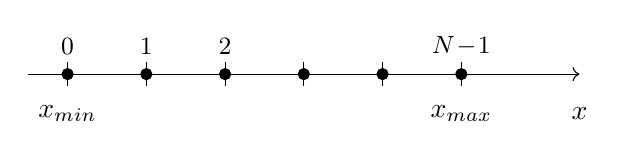
\begin{tikzpicture}
%\draw[fill=gray!23,gray!23](0,0) rectangle (8,2);
%\draw[step=0.5cm,gray,very thin] (0,0) grid (8,2); %background grid
\draw [->] (0.5,1) -- (7.5,1);
\draw[-] (1,0.85)--(1,1.15);
\draw[-] (2,0.85)--(2,1.15);
\draw[-] (3,0.85)--(3,1.15);
\draw[-] (4,0.85)--(4,1.15);
\draw[-] (5,0.85)--(5,1.15);
\draw[-] (6,0.85)--(6,1.15);
\node[] at (1,0.5) {$x_{min}$};
\node[] at (6,0.5) {$x_{max}$};
\node[] at (7.5,0.5) {$x$};
\draw[black,fill=black] (1,1)   circle (2pt);
\draw[black,fill=black] (2,1)   circle (2pt);
\draw[black,fill=black] (3,1)   circle (2pt);
\draw[black,fill=black] (4,1)   circle (2pt);
\draw[black,fill=black] (5,1)   circle (2pt);
\draw[black,fill=black] (6,1)   circle (2pt);
\node[] at (1,1.35) {\small 0};
\node[] at (2,1.35) {\small 1};
\node[] at (3,1.35) {\small 2};
\node[] at (6,1.35) {\small $N\!-\!1$};
\end{tikzpicture}
\end{center}

\noindent In this case the length of the domain is $L_x=x_{max}-x_{min}$, and the above code becomes:
\begin{lstlisting}
import numpy as np
N=10
xmin=-4
xmax=3
h=(xmax-xmin)/(N-1)
x=np.zeros(N,dtype=np.float64)
for i in range(0,N):
    x[i]=xmin+i*h
\end{lstlisting}
Note the presence of $x_{min}$ in the last line! 

\vspace{.8cm}

Unfortunately the world is definitely not one-dimensional, so 
I may want to build a two-dimensional grid spanning the domain 
$[0,L_x]\times[0,L_y]$ as depicted here:



\begin{center}
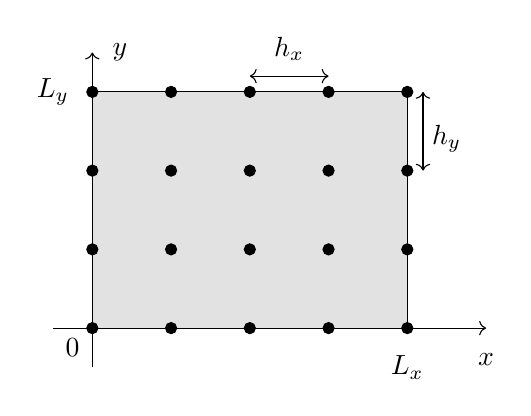
\begin{tikzpicture}
\draw[fill=gray!23,gray!23](1,1) rectangle (5,4);
%\draw[step=0.5cm,gray,very thin] (0,0) grid (7,5); 
\draw [->] (0.5,1) -- (6,1);
\draw [->] (1,0.5) -- (1,4.5);
\node[] at (0.75,0.75) {$0$};
\node[] at (5,0.5) {$L_x$};
\node[] at (0.5,4) {$L_y$};
\node[] at (6,0.6) {$x$};
\node[] at (1.35,4.5) {$y$};
\draw[-] (1,1)--(5,1)--(5,4)--(1,4)--cycle;
\draw[black,fill=black] (1,1)   circle (2pt);
\draw[black,fill=black] (2,1)   circle (2pt);
\draw[black,fill=black] (3,1)   circle (2pt);
\draw[black,fill=black] (4,1)   circle (2pt);
\draw[black,fill=black] (5,1)   circle (2pt);
\draw[black,fill=black] (1,2)   circle (2pt);
\draw[black,fill=black] (2,2)   circle (2pt);
\draw[black,fill=black] (3,2)   circle (2pt);
\draw[black,fill=black] (4,2)   circle (2pt);
\draw[black,fill=black] (5,2)   circle (2pt);
\draw[black,fill=black] (1,3)   circle (2pt);
\draw[black,fill=black] (2,3)   circle (2pt);
\draw[black,fill=black] (3,3)   circle (2pt);
\draw[black,fill=black] (4,3)   circle (2pt);
\draw[black,fill=black] (5,3)   circle (2pt);
\draw[black,fill=black] (1,4)   circle (2pt);
\draw[black,fill=black] (2,4)   circle (2pt);
\draw[black,fill=black] (3,4)   circle (2pt);
\draw[black,fill=black] (4,4)   circle (2pt);
\draw[black,fill=black] (5,4)   circle (2pt);
\draw[<->] (5.2,3)--(5.2,4);
\draw[<->] (3,4.2)--(4,4.2);
\node[] at (3.5,4.55) {$h_x$};
\node[] at (5.5,3.4) {$h_y$};
\end{tikzpicture}
\end{center}

\noindent There are now $N=N_x \times N_y$ nodes in the mesh, 
and we need to define the mesh spacing in both the $x$ and $y$
direction:
\[
h_x = \frac{L_x}{N_x-1}
\qquad\qquad
h_y = \frac{L_y}{N_y-1}
\]
From our experience with the 1D case, it seems logical to 
resort to a double for loop, one in the $x$ direction, 
one in the $y$ direction. 
However we must now make a decision as to which loop is inside the other (inner loop vs. outer loop). In essence, I must decide between 
\begin{lstlisting}
#approach 1
for i in range(0,Nx):
    for j in range(0,Ny):
\end{lstlisting}
and
\begin{lstlisting}
#approach 2
for j in range(0,Ny):
    for i in range(0,Nx):
\end{lstlisting}
As it turns out, I need not decide, both options are equally valid as we will see.
I now fix $N_x=4$ and $N_y=3$ so that the mesh contains 12 nodes:

\begin{center}
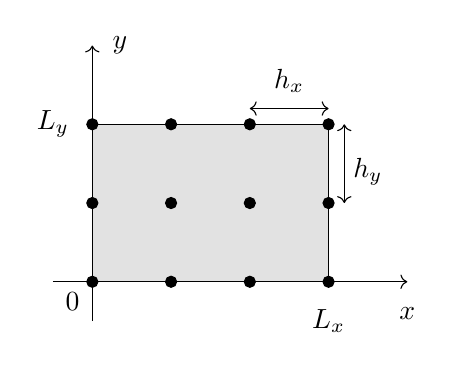
\begin{tikzpicture}
\draw[fill=gray!23,gray!23](1,1) rectangle (4,3);
%\draw[step=0.5cm,gray,very thin] (0,0) grid (7,5); 
\draw [->] (0.5,1) -- (5,1);
\draw [->] (1,0.5) -- (1,4);
\node[] at (0.75,0.75) {$0$};
\node[] at (4,0.5) {$L_x$};
\node[] at (0.5,3) {$L_y$};
\node[] at (5,0.6) {$x$};
\node[] at (1.35,4) {$y$};
\draw[-] (1,1)--(4,1)--(4,3)--(1,3)--cycle;
\draw[black,fill=black] (1,1)   circle (2pt);
\draw[black,fill=black] (2,1)   circle (2pt);
\draw[black,fill=black] (3,1)   circle (2pt);
\draw[black,fill=black] (4,1)   circle (2pt);
\draw[black,fill=black] (1,2)   circle (2pt);
\draw[black,fill=black] (2,2)   circle (2pt);
\draw[black,fill=black] (3,2)   circle (2pt);
\draw[black,fill=black] (4,2)   circle (2pt);
\draw[black,fill=black] (1,3)   circle (2pt);
\draw[black,fill=black] (2,3)   circle (2pt);
\draw[black,fill=black] (3,3)   circle (2pt);
\draw[black,fill=black] (4,3)   circle (2pt);
\draw[<->] (4.2,2)--(4.2,3);
\draw[<->] (3,3.2)--(4,3.2);
\node[] at (3.5,3.55) {$h_x$};
\node[] at (4.5,2.4) {$h_y$};
\end{tikzpicture}
\end{center}

\noindent Looking at approach \#1, I can include a print statement inside the loops as follows:
\begin{lstlisting}
#option 1
Nx=4
Ny=3
for i in range(0,Nx):
    for j in range(0,Ny):
        print('i=',i,'; j=',j)
\end{lstlisting}
If I was to run this code it would display (I first exhaust the $j$ values from the inner most loop before I switch to a different $i$ value):
\begin{lstlisting}
i= 0  ; j= 0
i= 0  ; j= 1
i= 0  ; j= 2
i= 1  ; j= 0
i= 1  ; j= 1
i= 1  ; j= 2
i= 2  ; j= 0
i= 2  ; j= 1
i= 2  ; j= 2
i= 3  ; j= 0
i= 3  ; j= 1
i= 3  ; j= 2
\end{lstlisting}
This means that the code is going through the nodes in the following order:
\begin{center}
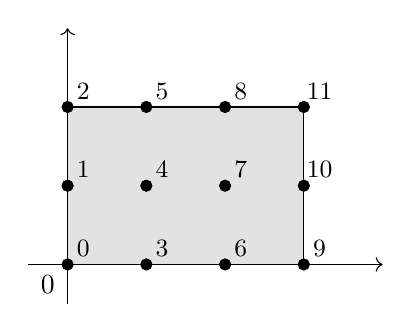
\begin{tikzpicture}
\draw[fill=gray!23,gray!23](1,1) rectangle (4,3);
%\draw[step=0.5cm,gray,very thin] (0,0) grid (7,5); 
\draw [->] (0.5,1) -- (5,1);
\draw [->] (1,0.5) -- (1,4);
\node[] at (0.75,0.75) {$0$};
\draw[-] (1,1)--(4,1)--(4,3)--(1,3)--cycle;
\draw[black,fill=black] (1,1)   circle (2pt);
\draw[black,fill=black] (2,1)   circle (2pt);
\draw[black,fill=black] (3,1)   circle (2pt);
\draw[black,fill=black] (4,1)   circle (2pt);
\draw[black,fill=black] (1,2)   circle (2pt);
\draw[black,fill=black] (2,2)   circle (2pt);
\draw[black,fill=black] (3,2)   circle (2pt);
\draw[black,fill=black] (4,2)   circle (2pt);
\draw[black,fill=black] (1,3)   circle (2pt);
\draw[black,fill=black] (2,3)   circle (2pt);
\draw[black,fill=black] (3,3)   circle (2pt);
\draw[black,fill=black] (4,3)   circle (2pt);
\node[] at (1.2,1.2) {\small $0$};
\node[] at (2.2,1.2) {\small $3$};
\node[] at (3.2,1.2) {\small $6$};
\node[] at (4.2,1.2) {\small $9$};
\node[] at (1.2,2.2) {\small $1$};
\node[] at (2.2,2.2) {\small $4$};
\node[] at (3.2,2.2) {\small $7$};
\node[] at (4.2,2.2) {\small $10$};
\node[] at (1.2,3.2) {\small $2$};
\node[] at (2.2,3.2) {\small $5$};
\node[] at (3.2,3.2) {\small $8$};
\node[] at (4.2,3.2) {\small $11$};
\end{tikzpicture}
\end{center}



Turning now to approach \#2, the same print statement will now yield:
\begin{lstlisting}
i= 0 ; j= 0
i= 1 ; j= 0
i= 2 ; j= 0
i= 3 ; j= 0
i= 0 ; j= 1
i= 1 ; j= 1
i= 2 ; j= 1
i= 3 ; j= 1
i= 0 ; j= 2
i= 1 ; j= 2
i= 2 ; j= 2
i= 3 ; j= 2
\end{lstlisting}
and this corresponds then to the following order: 
\begin{center}
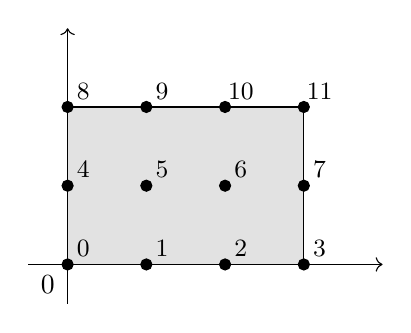
\begin{tikzpicture}
\draw[fill=gray!23,gray!23](1,1) rectangle (4,3);
%\draw[step=0.5cm,gray,very thin] (0,0) grid (7,5); 
\draw [->] (0.5,1) -- (5,1);
\draw [->] (1,0.5) -- (1,4);
\node[] at (0.75,0.75) {$0$};
\draw[-] (1,1)--(4,1)--(4,3)--(1,3)--cycle;
\draw[black,fill=black] (1,1)   circle (2pt);
\draw[black,fill=black] (2,1)   circle (2pt);
\draw[black,fill=black] (3,1)   circle (2pt);
\draw[black,fill=black] (4,1)   circle (2pt);
\draw[black,fill=black] (1,2)   circle (2pt);
\draw[black,fill=black] (2,2)   circle (2pt);
\draw[black,fill=black] (3,2)   circle (2pt);
\draw[black,fill=black] (4,2)   circle (2pt);
\draw[black,fill=black] (1,3)   circle (2pt);
\draw[black,fill=black] (2,3)   circle (2pt);
\draw[black,fill=black] (3,3)   circle (2pt);
\draw[black,fill=black] (4,3)   circle (2pt);
\node[] at (1.2,1.2) {\small $0$};
\node[] at (2.2,1.2) {\small $1$};
\node[] at (3.2,1.2) {\small $2$};
\node[] at (4.2,1.2) {\small $3$};
\node[] at (1.2,2.2) {\small $4$};
\node[] at (2.2,2.2) {\small $5$};
\node[] at (3.2,2.2) {\small $6$};
\node[] at (4.2,2.2) {\small $7$};
\node[] at (1.2,3.2) {\small $8$};
\node[] at (2.2,3.2) {\small $9$};
\node[] at (3.2,3.2) {\small $10$};
\node[] at (4.2,3.2) {\small $11$};
\end{tikzpicture}
\end{center}

\noindent In the end, we see that both approaches yield a valid 
numbering scheme, one is 'lines first' , the other 'columns first'.

In what follows I focus on approach \#2, only because it seems more 'natural' to me than the other one (it goes from left to right, then bottom to top). 
Our proto-code then looks like this:
\begin{lstlisting}
Lx=10
Ly=8
Nx=4
Ny=3
N=Nx*Ny
hx=Lx/(Nx-1)
hy=Ly/(Ny-1)
x=np.zeros(N,dtype=np.float64)
y=np.zeros(N,dtype=np.float64)
for j in range(0,Ny):
    for i in range(0,Nx):
        x[?]=i*hx
        y[?]=j*hy
\end{lstlisting}
Note that I have left two question marks. One may want to replace these by $i$ and $j$, 
following our experience in the 1D case. However, remember that $i$ ($j$) ranges between 
$0$ and $N_x-1=3$ ($0$ and $N_y-1=2$ respectively) but we need to assign and store the 
coordinates of all 12 nodes. 

So what should I write instead of question marks? Effectively, I need some form of counter 
so that every time the inner loop is executed the counter is incremented by one. 
When all $i,j$ combinations are exhausted this counter should have reached the 
last node. Such a counter can be implemented as follows:
\begin{lstlisting}
counter=0
for j in range(0,Ny):
    for i in range(0,Nx):
        print('counter=',counter,'i=',i,'; j=',j,j*Nx+i)
        counter+=1
\end{lstlisting}
It must be initialised to zero, and it is incremented $N_x \cdot N_y$ times.
Running this code would yield 
\begin{lstlisting}
counter=  0 i= 0 ; j= 0
counter=  1 i= 1 ; j= 0
counter=  2 i= 2 ; j= 0
counter=  3 i= 3 ; j= 0
counter=  4 i= 0 ; j= 1
counter=  5 i= 1 ; j= 1
counter=  6 i= 2 ; j= 1
counter=  7 i= 3 ; j= 1
counter=  8 i= 0 ; j= 2
counter=  9 i= 1 ; j= 2
counter= 10 i= 2 ; j= 2
counter= 11 i= 3 ; j= 2
\end{lstlisting}
We see that the counter takes all 12 values between 0 and 11, so it is the index I am looking for. Finally, the 2D code (or approach \#2) looks like:
\begin{lstlisting}
Lx=10
Ly=8
Nx=4
Ny=3
N=Nx*Ny
hx=Lx/(Nx-1)
hy=Ly/(Ny-1)
x=np.zeros(N,dtype=np.float64)
y=np.zeros(N,dtype=np.float64)
counter=0
for j in range(0,Ny):
    for i in range(0,Nx):
        x[counter]=i*hx
        y[counter]=j*hy
        counter+=1
\end{lstlisting}
It is trivial to verify that one can swap the two lines with the 'for' statements to obtain the approach \#1 version of the code.

Before I move to the three-dimensional case, I wish to mention a slightly different 
approach than the 'counter' one. 
Looking back at the numbering generated by approach \#2, it is easy to see that the node number (i.e. a value between 0 and 11)
can be also computed with $j\cdot N_x+i$. You can indeed verify that this expression yields the same values as the counter here above for all the $i,j$ combinations. However one must realise that this formula is not valid for approach \#1. The code then becomes:
\begin{lstlisting}
Lx=10
Ly=8
Nx=4
Ny=3
N=Nx*Ny
hx=Lx/(Nx-1)
hy=Ly/(Ny-1)
x=np.zeros(N,dtype=np.float64)
y=np.zeros(N,dtype=np.float64)
for j in range(0,Ny):
    for i in range(0,Nx):
        x[j*Nx+i]=i*hx
        y[j*Nx+i]=j*hy
\end{lstlisting}

Also, if the domain is not $[0,L_x]\times[0,L_y]$ but
$[x_{min},x_{max}]\times[y_{min},y_{max}]$, the code becomes
\begin{lstlisting}
xmin=-3
xmax=5
ymin=-1
ymax=4
Nx=4
Ny=3
N=Nx*Ny
hx=(xmax-xmin)/(Nx-1)
hy=(ymax-ymin)/(Ny-1)
x=np.zeros(N,dtype=np.float64)
y=np.zeros(N,dtype=np.float64)
for j in range(0,Ny):
    for i in range(0,Nx):
        x[j*Nx+i]=xmin+i*hx
        y[j*Nx+i]=ymin+j*hy
\end{lstlisting}

\vspace{.8cm}

Extending the codes above to three-dimensions is rather trivial, especially when the counter approach 
is used. One must simply be aware of the order of the loops (there are 3\! =6 approaches).
\begin{lstlisting}
xmin=-3
xmax=5
ymin=-1
ymax=4
zmin=1
zmax=6
Nx=4
Ny=3
Nz=5
N=Nx*Ny*Nz
hx=(xmax-xmin)/(Nx-1)
hy=(ymax-ymin)/(Ny-1)
hz=(zmax-zmin)/(Nz-1)
x=np.zeros(N,dtype=np.float64)
y=np.zeros(N,dtype=np.float64)
z=np.zeros(N,dtype=np.float64)
counter
for k in range(0,Nz):
    for j in range(0,Ny):
        for i in range(0,Nx):
            x[counter]=xmin+i*hx
            y[counter]=ymin+j*hy
            z[counter]=zmin+k*hz
            counter+=1
\end{lstlisting}
You will find near identical codes in (for example) Stone 1 and 10.

\vspace{.8cm}

In some cases, we wish to store the coordinates of the mesh nodes because the nodes 
make a regular grid of quadrilaterals on which ODEs or PDEs will be solved:

\begin{center}
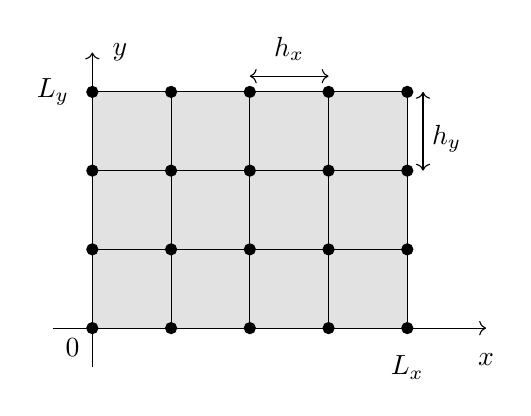
\begin{tikzpicture}
\draw[fill=gray!23,gray!23](1,1) rectangle (5,4);
%\draw[step=0.5cm,gray,very thin] (0,0) grid (7,5); 
\draw [->] (0.5,1) -- (6,1);
\draw [->] (1,0.5) -- (1,4.5);
\node[] at (0.75,0.75) {$0$};
\node[] at (5,0.5) {$L_x$};
\node[] at (0.5,4) {$L_y$};
\node[] at (6,0.6) {$x$};
\node[] at (1.35,4.5) {$y$};
\draw[-] (1,1)--(5,1)--(5,4)--(1,4)--cycle;
\draw[-] (1,2)--(5,2);
\draw[-] (1,3)--(5,3);
\draw[-] (2,1)--(2,4);
\draw[-] (3,1)--(3,4);
\draw[-] (4,1)--(4,4);
\draw[black,fill=black] (1,1)   circle (2pt);
\draw[black,fill=black] (2,1)   circle (2pt);
\draw[black,fill=black] (3,1)   circle (2pt);
\draw[black,fill=black] (4,1)   circle (2pt);
\draw[black,fill=black] (5,1)   circle (2pt);
\draw[black,fill=black] (1,2)   circle (2pt);
\draw[black,fill=black] (2,2)   circle (2pt);
\draw[black,fill=black] (3,2)   circle (2pt);
\draw[black,fill=black] (4,2)   circle (2pt);
\draw[black,fill=black] (5,2)   circle (2pt);
\draw[black,fill=black] (1,3)   circle (2pt);
\draw[black,fill=black] (2,3)   circle (2pt);
\draw[black,fill=black] (3,3)   circle (2pt);
\draw[black,fill=black] (4,3)   circle (2pt);
\draw[black,fill=black] (5,3)   circle (2pt);
\draw[black,fill=black] (1,4)   circle (2pt);
\draw[black,fill=black] (2,4)   circle (2pt);
\draw[black,fill=black] (3,4)   circle (2pt);
\draw[black,fill=black] (4,4)   circle (2pt);
\draw[black,fill=black] (5,4)   circle (2pt);
\draw[<->] (5.2,3)--(5.2,4);
\draw[<->] (3,4.2)--(4,4.2);
\node[] at (3.5,4.55) {$h_x$};
\node[] at (5.5,3.4) {$h_y$};
\end{tikzpicture}
\end{center}

There are $N_x$ nodes in the $x$ direction but only $N_x-1$ cells/elements\footnote{Because of my 
bias towards the Finite Element Method, I will refer to these as elements.}. 
Likewise there are $N_y$ nodes in the $y$ direction but only $N_y-1$ cells/elements.
In total there are $N_e=(N_x-1)(N_y-1)$ elements. 
As for the cell center nodes, we must adopt a systematic way of numbering them. 
If I keep using approach \#2 for the nodes, the following numbering of 
{\color{teal}elements} seems natural:

\begin{center}
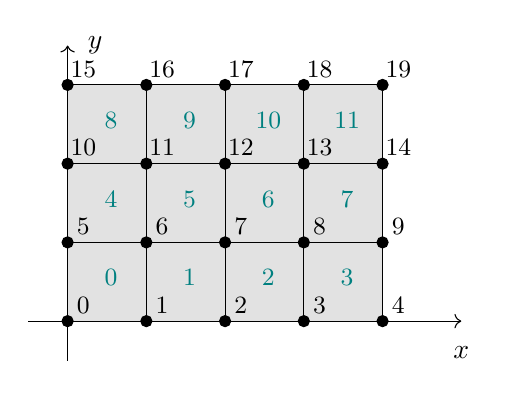
\begin{tikzpicture}
\draw[fill=gray!23,gray!23](1,1) rectangle (5,4);
%\draw[step=0.5cm,gray,very thin] (0,0) grid (7,5); 
\draw [->] (0.5,1) -- (6,1);
\draw [->] (1,0.5) -- (1,4.5);
\node[] at (6,0.6) {$x$};
\node[] at (1.35,4.5) {$y$};
\draw[-] (1,1)--(5,1)--(5,4)--(1,4)--cycle;
\draw[-] (1,2)--(5,2);
\draw[-] (1,3)--(5,3);
\draw[-] (2,1)--(2,4);
\draw[-] (3,1)--(3,4);
\draw[-] (4,1)--(4,4);
\draw[black,fill=black] (1,1)   circle (2pt);
\draw[black,fill=black] (2,1)   circle (2pt);
\draw[black,fill=black] (3,1)   circle (2pt);
\draw[black,fill=black] (4,1)   circle (2pt);
\draw[black,fill=black] (5,1)   circle (2pt);
\draw[black,fill=black] (1,2)   circle (2pt);
\draw[black,fill=black] (2,2)   circle (2pt);
\draw[black,fill=black] (3,2)   circle (2pt);
\draw[black,fill=black] (4,2)   circle (2pt);
\draw[black,fill=black] (5,2)   circle (2pt);
\draw[black,fill=black] (1,3)   circle (2pt);
\draw[black,fill=black] (2,3)   circle (2pt);
\draw[black,fill=black] (3,3)   circle (2pt);
\draw[black,fill=black] (4,3)   circle (2pt);
\draw[black,fill=black] (5,3)   circle (2pt);
\draw[black,fill=black] (1,4)   circle (2pt);
\draw[black,fill=black] (2,4)   circle (2pt);
\draw[black,fill=black] (3,4)   circle (2pt);
\draw[black,fill=black] (4,4)   circle (2pt);
\draw[black,fill=black] (5,4)   circle (2pt);
\node[] at (1.2,1.2) {\small $0$};
\node[] at (2.2,1.2) {\small $1$};
\node[] at (3.2,1.2) {\small $2$};
\node[] at (4.2,1.2) {\small $3$};
\node[] at (5.2,1.2) {\small $4$};
\node[] at (1.2,2.2) {\small $5$};
\node[] at (2.2,2.2) {\small $6$};
\node[] at (3.2,2.2) {\small $7$};
\node[] at (4.2,2.2) {\small $8$};
\node[] at (5.2,2.2) {\small $9$};
\node[] at (1.2,3.2) {\small $10$};
\node[] at (2.2,3.2) {\small $11$};
\node[] at (3.2,3.2) {\small $12$};
\node[] at (4.2,3.2) {\small $13$};
\node[] at (5.2,3.2) {\small $14$};
\node[] at (1.2,4.2) {\small $15$};
\node[] at (2.2,4.2) {\small $16$};
\node[] at (3.2,4.2) {\small $17$};
\node[] at (4.2,4.2) {\small $18$};
\node[] at (5.2,4.2) {\small $19$};
\node[] at (1.55,1.55) {\color{teal} \small $0$};
\node[] at (2.55,1.55) {\color{teal} \small $1$};
\node[] at (3.55,1.55) {\color{teal} \small $2$};
\node[] at (4.55,1.55) {\color{teal} \small $3$};
\node[] at (1.55,2.55) {\color{teal} \small $4$};
\node[] at (2.55,2.55) {\color{teal} \small $5$};
\node[] at (3.55,2.55) {\color{teal} \small $6$};
\node[] at (4.55,2.55) {\color{teal} \small $7$};
\node[] at (1.55,3.55) {\color{teal} \small $8$};
\node[] at (2.55,3.55) {\color{teal} \small $9$};
\node[] at (3.55,3.55) {\color{teal} \small $10$};
\node[] at (4.55,3.55) {\color{teal} \small $11$};
\end{tikzpicture}
\end{center}

In some applications we want to also store the coordinates of the center of all cells, i.e. the $N_e$ coordinates of {\color{teal} these} points:

\begin{center}
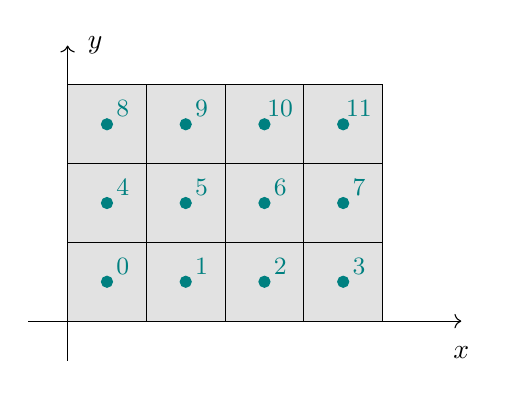
\begin{tikzpicture}
\draw[fill=gray!23,gray!23](1,1) rectangle (5,4);
%\draw[step=0.5cm,gray,very thin] (0,0) grid (7,5); 
\draw [->] (0.5,1) -- (6,1);
\draw [->] (1,0.5) -- (1,4.5);
\node[] at (6,0.6) {$x$};
\node[] at (1.35,4.5) {$y$};
\draw[-] (1,1)--(5,1)--(5,4)--(1,4)--cycle;
\draw[-] (1,2)--(5,2);
\draw[-] (1,3)--(5,3);
\draw[-] (2,1)--(2,4);
\draw[-] (3,1)--(3,4);
\draw[-] (4,1)--(4,4);
\draw[black,fill=black,color=teal] (1.5,1.5)   circle (2pt);
\draw[black,fill=black,color=teal] (2.5,1.5)   circle (2pt);
\draw[black,fill=black,color=teal] (3.5,1.5)   circle (2pt);
\draw[black,fill=black,color=teal] (4.5,1.5)   circle (2pt);
\draw[black,fill=black,color=teal] (1.5,2.5)   circle (2pt);
\draw[black,fill=black,color=teal] (2.5,2.5)   circle (2pt);
\draw[black,fill=black,color=teal] (3.5,2.5)   circle (2pt);
\draw[black,fill=black,color=teal] (4.5,2.5)   circle (2pt);
\draw[black,fill=black,color=teal] (1.5,3.5)   circle (2pt);
\draw[black,fill=black,color=teal] (2.5,3.5)   circle (2pt);
\draw[black,fill=black,color=teal] (3.5,3.5)   circle (2pt);
\draw[black,fill=black,color=teal] (4.5,3.5)   circle (2pt);
\node[] at (1.7,1.7) {\color{teal} \small $0$};
\node[] at (2.7,1.7) {\color{teal} \small $1$};
\node[] at (3.7,1.7) {\color{teal} \small $2$};
\node[] at (4.7,1.7) {\color{teal} \small $3$};
\node[] at (1.7,2.7) {\color{teal} \small $4$};
\node[] at (2.7,2.7) {\color{teal} \small $5$};
\node[] at (3.7,2.7) {\color{teal} \small $6$};
\node[] at (4.7,2.7) {\color{teal} \small $7$};
\node[] at (1.7,3.7) {\color{teal} \small $8$};
\node[] at (2.7,3.7) {\color{teal} \small $9$};
\node[] at (3.7,3.7) {\color{teal} \small $10$};
\node[] at (4.7,3.7) {\color{teal} \small $11$};
\end{tikzpicture}
\end{center}
Given this numbering these points form a regular grid:
\begin{center}
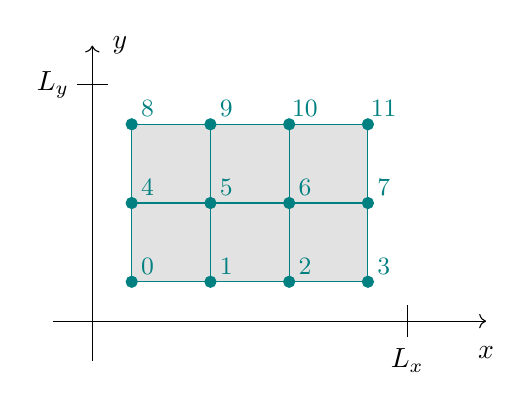
\begin{tikzpicture}
\draw[fill=gray!23,gray!23](1.5,1.5) rectangle (4.5,3.5);
%\draw[step=0.5cm,gray,very thin] (0,0) grid (7,5); 
\draw [->] (0.5,1) -- (6,1);
\draw [->] (1,0.5) -- (1,4.5);
\node[] at (6,0.6) {$x$};
\node[] at (1.35,4.5) {$y$};
\draw[-,teal] (1.5,1.5)--(4.5,1.5)--(4.5,3.5)--(1.5,3.5)--cycle;
\draw[-,teal] (1.5,2.5)--(4.5,2.5);
\draw[-,teal] (2.5,1.5)--(2.5,3.5);
\draw[-,teal] (3.5,1.5)--(3.5,3.5);
\draw[black,fill=black,color=teal] (1.5,1.5)   circle (2pt);
\draw[black,fill=black,color=teal] (2.5,1.5)   circle (2pt);
\draw[black,fill=black,color=teal] (3.5,1.5)   circle (2pt);
\draw[black,fill=black,color=teal] (4.5,1.5)   circle (2pt);
\draw[black,fill=black,color=teal] (1.5,2.5)   circle (2pt);
\draw[black,fill=black,color=teal] (2.5,2.5)   circle (2pt);
\draw[black,fill=black,color=teal] (3.5,2.5)   circle (2pt);
\draw[black,fill=black,color=teal] (4.5,2.5)   circle (2pt);
\draw[black,fill=black,color=teal] (1.5,3.5)   circle (2pt);
\draw[black,fill=black,color=teal] (2.5,3.5)   circle (2pt);
\draw[black,fill=black,color=teal] (3.5,3.5)   circle (2pt);
\draw[black,fill=black,color=teal] (4.5,3.5)   circle (2pt);
\node[] at (1.7,1.7) {\color{teal} \small $0$};
\node[] at (2.7,1.7) {\color{teal} \small $1$};
\node[] at (3.7,1.7) {\color{teal} \small $2$};
\node[] at (4.7,1.7) {\color{teal} \small $3$};
\node[] at (1.7,2.7) {\color{teal} \small $4$};
\node[] at (2.7,2.7) {\color{teal} \small $5$};
\node[] at (3.7,2.7) {\color{teal} \small $6$};
\node[] at (4.7,2.7) {\color{teal} \small $7$};
\node[] at (1.7,3.7) {\color{teal} \small $8$};
\node[] at (2.7,3.7) {\color{teal} \small $9$};
\node[] at (3.7,3.7) {\color{teal} \small $10$};
\node[] at (4.7,3.7) {\color{teal} \small $11$};
\draw[-] (5,0.8)--(5,1.2);
\draw[-] (0.8,4)--(1.2,4);
\node[] at (5,0.5) {$L_x$};
\node[] at (0.5,4) {$L_y$};
\end{tikzpicture}
\end{center}
This 'new' domain is bound by $x'_{min}=h_x/2$, $x'_{max}=L_x-h_x/2$ in 
the $x$ direction and $y'_{min}=h/2$, $y'_{max}=L_y-h_y/2$ in the $y$ direction. We note that the spacings $h_x$ and $h_y$ between the centers is the same as for the nodes. 
We store the coordinates $(x_c,y_c)$ of the cell centers in two arrays of length $N_e$ and the code is then simply

\begin{lstlisting}
Lx=9
Ly=7
Nx=4
Ny=3
N=Nx*Ny
hx=(xmax-xmin)/(Nx-1)
hy=(ymax-ymin)/(Ny-1)
#mesh nodes coordinates
x=np.zeros(N,dtype=np.float64)
y=np.zeros(N,dtype=np.float64)
counter=0
for j in range(0,Ny):
    for i in range(0,Nx):
        x[counter]=i*hx
        y[counter]=j*hy
        counter+=1
#cell centers coordinates
Ne=(Nx-1)*(Ny-1)
xc=np.zeros(Ne,dtype=np.float64)
yc=np.zeros(Ne,dtype=np.float64)
xmin=hx/2
xmax=Lx-hx/2
ymin=hy/2
ymax=Ly-hy/2
counter=0
for j in range(0,Ny-1):
    for i in range(0,Nx-1):
        xc[counter]=xmin+i*hx
        yc[counter]=ymin+j*hy
        counter+=1
\end{lstlisting}

%--------------------------------------------
\subsection*{The connectivity array}

Let us consider 3 points in a plane:
\begin{center}
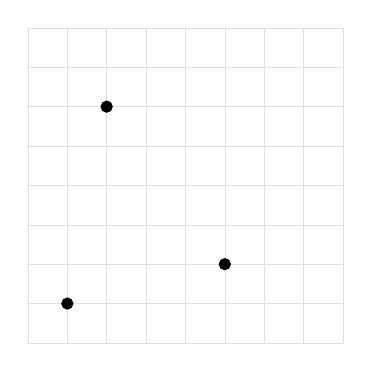
\begin{tikzpicture}
\draw[step=0.5cm,gray!25,very thin] (0.5,0.5) grid (4.5,4.5); 
\draw[black,fill=black] (1,1)   circle (2pt);
\draw[black,fill=black] (3,1.5)   circle (2pt);
\draw[black,fill=black] (1.5,3.5)   circle (2pt);
\end{tikzpicture}
\end{center}
Since they are not aligned they form a triangle:
\begin{center}
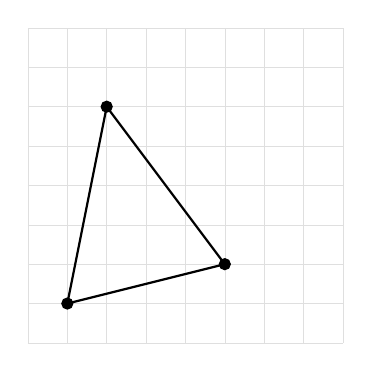
\begin{tikzpicture}
\draw[step=0.5cm,gray!25,very thin] (0.5,0.5) grid (4.5,4.5); 
\draw[black,fill=black] (1,1)   circle (2pt);
\draw[black,fill=black] (3,1.5)   circle (2pt);
\draw[black,fill=black] (1.5,3.5)   circle (2pt);
\draw[-,thick] (1,1)--(3,1.5)--(1.5,3.5)--cycle;
\end{tikzpicture}
\end{center}
When it comes to assigning these points an identity (or a number), I can arbitrarily assign them the following numbers:
\begin{center}
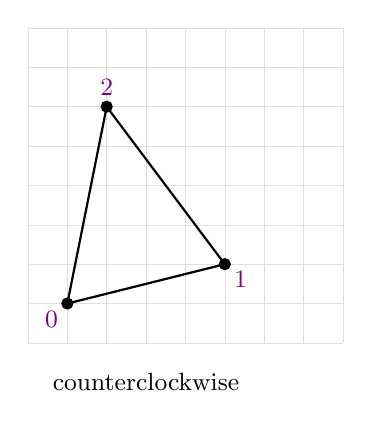
\begin{tikzpicture}
\draw[step=0.5cm,gray!25,very thin] (0.5,0.5) grid (4.5,4.5); 
\draw[black,fill=black] (1,1)   circle (2pt);
\draw[black,fill=black] (3,1.5)   circle (2pt);
\draw[black,fill=black] (1.5,3.5)   circle (2pt);
\draw[-,thick] (1,1)--(3,1.5)--(1.5,3.5)--cycle;
\node[] at (0.8,0.8) {\small \color{violet}0};
\node[] at (3.2,1.3) {\small \color{violet}1};
\node[] at (1.5,3.75) {\small \color{violet}2};
\node[] at (2,0) {\small counterclockwise};
\end{tikzpicture}
\end{center}
This triangle is then made of nodes {\color{violet}0}, 
{\color{violet}1}, and {\color{violet}2}.

Let us now add one more point in the plane as follows:
\begin{center}
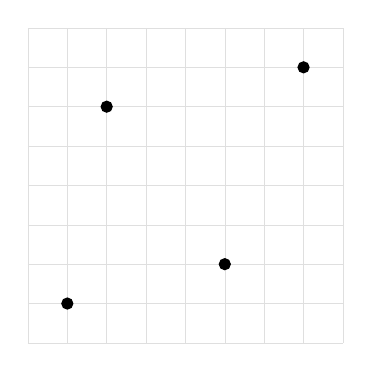
\begin{tikzpicture}
\draw[step=0.5cm,gray!25,very thin] (0.5,0.5) grid (4.5,4.5); 
\draw[black,fill=black] (1,1)   circle (2pt);
\draw[black,fill=black] (3,1.5)   circle (2pt);
\draw[black,fill=black] (1.5,3.5)   circle (2pt);
\draw[black,fill=black] (4,4)   circle (2pt);
\end{tikzpicture}
\end{center}
I will here number them as follows:
\begin{center}
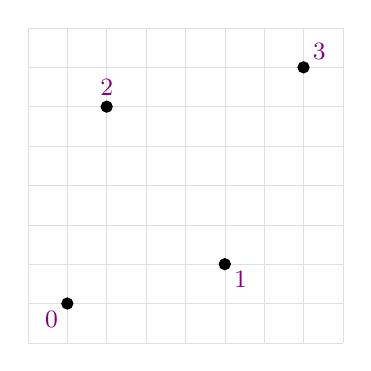
\begin{tikzpicture}
\draw[step=0.5cm,gray!25,very thin] (0.5,0.5) grid (4.5,4.5); 
\draw[black,fill=black] (1,1)   circle (2pt);
\draw[black,fill=black] (3,1.5)   circle (2pt);
\draw[black,fill=black] (1.5,3.5)   circle (2pt);
\draw[black,fill=black] (4,4)   circle (2pt);
\node[] at (0.8,0.8) {\small \color{violet}0};
\node[] at (3.2,1.3) {\small \color{violet}1};
\node[] at (1.5,3.75) {\small \color{violet}2};
\node[] at (4.2,4.2) {\small \color{violet}3};
\end{tikzpicture}
\end{center}

I can either decide to see them as the vertices of a quadrilateral, or
as the vertices of two triangles. However, there are two possibilities for the triangles:

\begin{center}
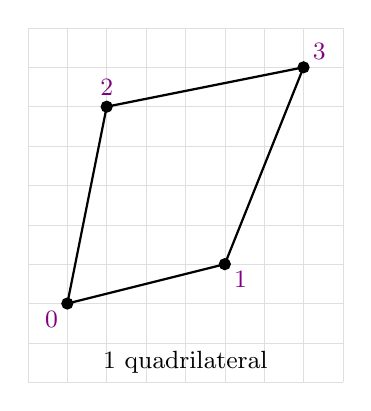
\begin{tikzpicture}
\draw[step=0.5cm,gray!25,very thin] (0.5,0) grid (4.5,4.5); 
\draw[black,fill=black] (1,1)   circle (2pt);
\draw[black,fill=black] (3,1.5)   circle (2pt);
\draw[black,fill=black] (1.5,3.5)   circle (2pt);
\draw[black,fill=black] (4,4)   circle (2pt);
\draw[-,thick] (1,1)--(3,1.5)--(4,4)--(1.5,3.5)--cycle;
\node[] at (0.8,0.8) {\small \color{violet}0};
\node[] at (3.2,1.3) {\small \color{violet}1};
\node[] at (1.5,3.75) {\small \color{violet}2};
\node[] at (4.2,4.2) {\small \color{violet}3};
\node[] at (2.5,0.25) {\small 1 quadrilateral};
\end{tikzpicture}
\hspace{1cm}
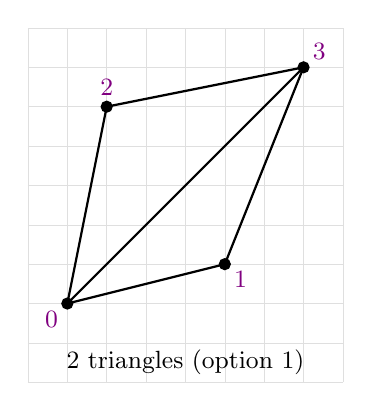
\begin{tikzpicture}
\draw[step=0.5cm,gray!25,very thin] (0.5,0) grid (4.5,4.5); 
\draw[black,fill=black] (1,1)   circle (2pt);
\draw[black,fill=black] (3,1.5)   circle (2pt);
\draw[black,fill=black] (1.5,3.5)   circle (2pt);
\draw[black,fill=black] (4,4)   circle (2pt);
\draw[-,thick] (1,1)--(3,1.5)--(4,4)--(1.5,3.5)--cycle;
\draw[-,thick] (1,1)--(4,4);
\node[] at (0.8,0.8) {\small \color{violet}0};
\node[] at (3.2,1.3) {\small \color{violet}1};
\node[] at (1.5,3.75) {\small \color{violet}2};
\node[] at (4.2,4.2) {\small \color{violet}3};
\node[] at (2.5,0.25) {\small 2 triangles (option 1)};
\end{tikzpicture}
\hspace{1cm}
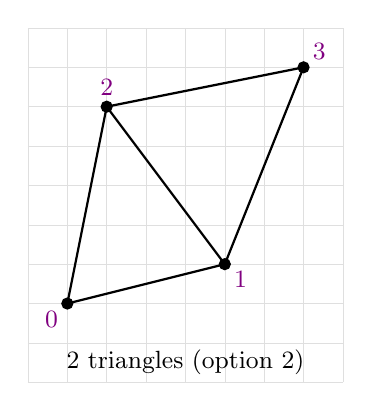
\begin{tikzpicture}
\draw[step=0.5cm,gray!25,very thin] (0.5,0) grid (4.5,4.5); 
\draw[black,fill=black] (1,1)   circle (2pt);
\draw[black,fill=black] (3,1.5)   circle (2pt);
\draw[black,fill=black] (1.5,3.5)   circle (2pt);
\draw[black,fill=black] (4,4)   circle (2pt);
\draw[-,thick] (1,1)--(3,1.5)--(4,4)--(1.5,3.5)--cycle;
\draw[-,thick] (3,1.5)--(1.5,3.5);
\node[] at (0.8,0.8) {\small \color{violet}0};
\node[] at (3.2,1.3) {\small \color{violet}1};
\node[] at (1.5,3.75) {\small \color{violet}2};
\node[] at (4.2,4.2) {\small \color{violet}3};
\node[] at (2.5,0.25) {\small 2 triangles (option 2)};
\end{tikzpicture}
\end{center}

When it comes to the quadrilateral, assuming a counterclockwise numbering, I can say that this quadrilaterals is then made of nodes 
{\color{violet}0}, {\color{violet}1},
{\color{violet}3} and {\color{violet}2}.
Note that I could also say it is made of nodes 
{\color{violet}3}, {\color{violet}2},
{\color{violet}0} and {\color{violet}1}.

Looking at the cases with 2 triangles I first need to label/number the triangles themselves:
\begin{center}
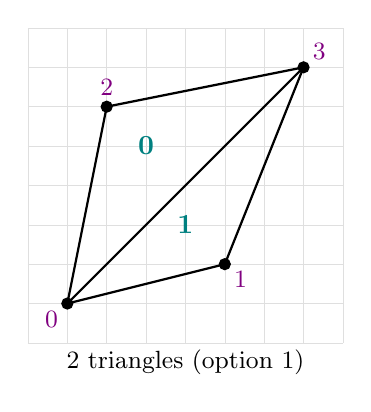
\begin{tikzpicture}
\draw[step=0.5cm,gray!25,very thin] (0.5,0.5) grid (4.5,4.5); 
\draw[black,fill=black] (1,1)   circle (2pt);
\draw[black,fill=black] (3,1.5)   circle (2pt);
\draw[black,fill=black] (1.5,3.5)   circle (2pt);
\draw[black,fill=black] (4,4)   circle (2pt);
\draw[-,thick] (1,1)--(3,1.5)--(4,4)--(1.5,3.5)--cycle;
\draw[-,thick] (1,1)--(4,4);
\node[] at (0.8,0.8) {\small \color{violet}0};
\node[] at (3.2,1.3) {\small \color{violet}1};
\node[] at (1.5,3.75) {\small \color{violet}2};
\node[] at (4.2,4.2) {\small \color{violet}3};
\node[] at (2,3) {\bf \color{teal}0};
\node[] at (2.5,2) {\bf \color{teal}1};
\node[] at (2.5,0.25) {\small 2 triangles (option 1)};
\end{tikzpicture}
\hspace{1cm}
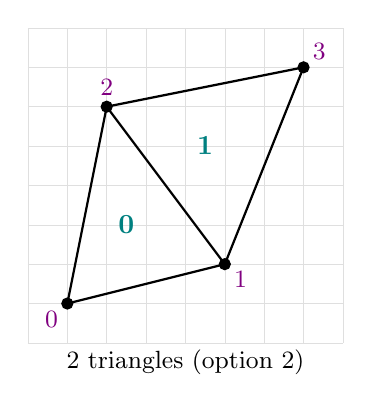
\begin{tikzpicture}
\draw[step=0.5cm,gray!25,very thin] (0.5,0.5) grid (4.5,4.5); 
\draw[black,fill=black] (1,1)   circle (2pt);
\draw[black,fill=black] (3,1.5)   circle (2pt);
\draw[black,fill=black] (1.5,3.5)   circle (2pt);
\draw[black,fill=black] (4,4)   circle (2pt);
\draw[-,thick] (1,1)--(3,1.5)--(4,4)--(1.5,3.5)--cycle;
\draw[-,thick] (3,1.5)--(1.5,3.5);
\node[] at (0.8,0.8) {\small \color{violet}0};
\node[] at (3.2,1.3) {\small \color{violet}1};
\node[] at (1.5,3.75) {\small \color{violet}2};
\node[] at (4.2,4.2) {\small \color{violet}3};
\node[] at (1.75,2) {\bf \color{teal}0};
\node[] at (2.75,3) {\bf \color{teal}1};
\node[] at (2.5,0.25) {\small 2 triangles (option 2)};
\end{tikzpicture}
\end{center}

In option 1, and still using a counterclockwise approach, triangle {\color{teal} 0} is made of nodes 
\{{\color{violet}0},{\color{violet}3},{\color{violet}2}\} and 
triangle {\color{teal} 1} is made of nodes 
\{{\color{violet}0},{\color{violet}1},{\color{violet}3}\}. 
In option 2, 
triangle {\color{teal} 0} is made of nodes 
\{{\color{violet}0},{\color{violet}1},{\color{violet}2}\} and 
triangle {\color{teal} 1} is made of nodes 
\{{\color{violet}1},{\color{violet}3},{\color{violet}2}\}. 

If I keep adding points, I will ultimately end up with a mesh which 
counts many quadrilaterals and/or triangles. In order to characterise this mesh, I need two numbers: $nel$, the number of elements (or cells) and $N$ the total number of vertices. However, this is not enough because I also need to know which vertex belongs to which element. 

Concretely, I need to store for each element a list of $m=3$ (triangles) or $m=4$ (quadrilaterals) numbers. The resulting array is often called the connectivity array. In FieldStone this array is always {\tt icon}, of size $m \times nel$.

In the cases above, $m=3$, $nel=2$, $N=4$ and 
\[
{\tt icon}_{\rm option\; 1}=
\left(
\begin{array}{cc}
{\color{violet}0}&{\color{violet}0}\\
{\color{violet}3}&{\color{violet}1}\\
{\color{violet}2}&{\color{violet}3}\\
\end{array}
\right)
\qquad
{\tt icon}_{\rm option\; 2}=
\left(
\begin{array}{cc}
{\color{violet}0}&{\color{violet}1}\\
{\color{violet}1}&{\color{violet}3}\\
{\color{violet}2}&{\color{violet}2}
\end{array}
\right)
\]
The way to understand these is as follows: for option 1,
\begin{itemize}
\item
icon[0,0]='the identity of node \#0 of element \#0' $\rightarrow$ {\color{violet}1}
\item
icon[1,0]='the identity of node \#1 of element \#0' $\rightarrow$ {\color{violet}4}
\item
icon[2,0]='the identity of node \#2 of element \#0' $\rightarrow$ {\color{violet}3}
\item
icon[0,1]='the identity of node \#0 of element \#1' $\rightarrow$ {\color{violet}1}
\item
icon[1,1]='the identity of node \#1 of element \#1' $\rightarrow$ {\color{violet}2}
\item
icon[2,1]='the identity of node \#2 of element \#1' $\rightarrow$ {\color{violet}4}
\end{itemize}

Finally, let us consider the following case:

\begin{center}
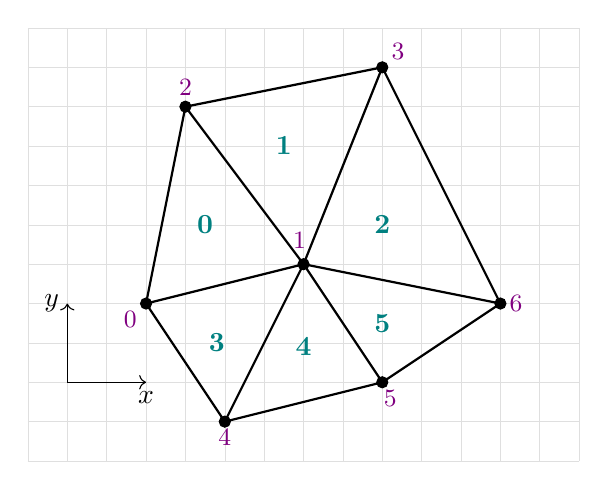
\begin{tikzpicture}
\draw[step=0.5cm,gray!25,very thin] (-0.5,-1) grid (6.5,4.5); 
\draw[black,fill=black] (1,1)   circle (2pt);
\draw[black,fill=black] (3,1.5)   circle (2pt);
\draw[black,fill=black] (1.5,3.5)   circle (2pt);
\draw[black,fill=black] (4,4)   circle (2pt);
\draw[black,fill=black] (5.5,1)   circle (2pt);
\draw[black,fill=black] (2.,-0.5)   circle (2pt);
\draw[black,fill=black] (4,0)   circle (2pt);

\draw[-,thick] (1,1)--(3,1.5)--(4,4)--(1.5,3.5)--cycle;
\draw[-,thick] (3,1.5)--(1.5,3.5);
\draw[-,thick] (3,1.5)--(5.5,1)--(4,4);
\draw[-,thick] (1,1)--(2,-0.5)--(4,0)--(5.5,1);
\draw[-,thick] (2,-0.5)--(3,1.5)--(4,0);
\node[] at (0.8,0.8) {\small \color{violet}0};
\node[] at (2.95,1.8) {\small \color{violet}1};
\node[] at (1.5,3.75) {\small \color{violet}2};
\node[] at (4.2,4.2) {\small \color{violet}3};
\node[] at (2,-0.7) {\small \color{violet}4};
\node[] at (4.1,-0.2) {\small \color{violet}5};
\node[] at (5.7,1) {\small \color{violet}6};

\node[] at (1.75,2) {\bf \color{teal}0};
\node[] at (2.75,3) {\bf \color{teal}1};
\node[] at (4,2) {\bf \color{teal}2};
\node[] at (1.9,0.5) {\bf \color{teal}3};
\node[] at (3,0.45) {\bf \color{teal}4};
\node[] at (4,0.75) {\bf \color{teal}5};


\draw[->] (0,0)--(1,0); 
\node[] at (1,-0.2) {$x$};
\draw[->] (0,0)--(0,1);
\node[] at (-0.2,1) {$y$};
\end{tikzpicture}
\end{center}
This mesh counts $nel=6$ elements/cells and $N=7$ points. 
The connectivity array is then of size $3\times 6$:
\[
{\tt icon}=
\left(
\begin{array}{cccccc}
{\color{violet}0}&{\color{violet}1}&{\color{violet}1}&{\color{violet}0}&{\color{violet}4}&{\color{violet}5}\\
{\color{violet}1}&{\color{violet}3}&{\color{violet}6}&{\color{violet}4}&{\color{violet}5}&{\color{violet}6}\\
{\color{violet}2}&{\color{violet}2}&{\color{violet}3}&{\color{violet}1}&{\color{violet}1}&{\color{violet}1}
\end{array}
\right)
\]
with 
\begin{align}
{\tt x}&=
\left(
\begin{array}{p{0.58cm}p{0.58cm}p{0.58cm}p{0.58cm}p{0.58cm}p{0.58cm}p{0.58cm}}
1 & 3 & 1.5 & 4 & 2 & 4 & 5.5
\end{array}
\right) \\
{\tt y}&=
\left(
\begin{array}{p{0.58cm}p{0.58cm}p{0.58cm}p{0.58cm}p{0.58cm}p{0.58cm}p{0.58cm}}
1 & 1.5 & 3.5 & 4 & -0.5 & 0 & 1
\end{array}
\right)
\end{align}

Let us then compute the barycenter coordinates of all triangles in arrays 
{\tt xb} and {\tt yb} of size $N=7$.
We need to loop over all triangles and for each compute the average of 
its nodes coordinates:
\begin{verbatim}
for iel in range(0,nel):
    xb[iel]=(x[icon[0,iel]]+x[icon[1,iel]]+x[icon[2,iel]])/3
    yb[iel]=(y[icon[0,iel]]+y[icon[1,iel]]+y[icon[2,iel]])/3
\end{verbatim}

The same concepts of course apply in 3D. In the case of tetrahedra then $m=4$ and in the case of hexahedra then $m=8$.

 %%%%%%%%%%%%%%%%%%%%%%%%%%%%%%%%%%%%%%%%%%%%%%%%%%%%%%%%%%%

\chapter{Manufactured solution ($Q_1\times P_0$+penalty)\label{f01}} %%%%%%%%%%%%%%%%%%%%%%%%%%%%%% 01
\begin{flushright} {\tiny {\color{gray} python\_codes/fieldstone\_01/text.tex}} \end{flushright}

\lstinputlisting[language=bash,basicstyle=\small]{python_codes/fieldstone_01/keywords.ascii}

\begin{center}

\fbox{\textbf{\huge \color{teal} P}}
\fbox{\textbf{\huge \color{purple} J}}
\fbox{\textbf{\huge \color{orange} F}}
Codes at \url{https://github.com/cedrict/fieldstone/tree/master/python_codes/fieldstone_01}
\end{center}

\par\noindent\rule{\textwidth}{0.4pt}

{\sl The python stone was developed in collaboration with Job Mos}. \index{contributors}{J. Mos}
{\sl The julia stone was developed by Jort Jansen.}. \index{contributors}{J. Jansen}

\par\noindent\rule{\textwidth}{0.4pt}
%%%%%%%%%%%%%%%%%%%%%%%%%%%%%%%%%%%%%%%%%%%%%%%%%%%%%%%%%%%%%%%%%%%%%%%%%%%%%%%%%%%%%%%%%%%%%%

This benchmark is taken from Donea \& Huerta (2003) \cite{dohu03} and is described fully in section \ref{mms1}. 
In order to illustrate the behavior of selected mixed finite elements in the solution 
of stationary Stokes flow,  we consider a two-dimensional problem 
in the square domain $\Omega=[0,1]\times[0,1]$, which possesses a closed-form analytical 
solution. 

\begin{center}
\includegraphics[width=10cm]{python_codes/fieldstone_01/results/errors.pdf}\\
{\captionfont Quadratic convergence for velocity error, 
linear convergence for pressure error, as expected.}
\end{center}

\begin{center}
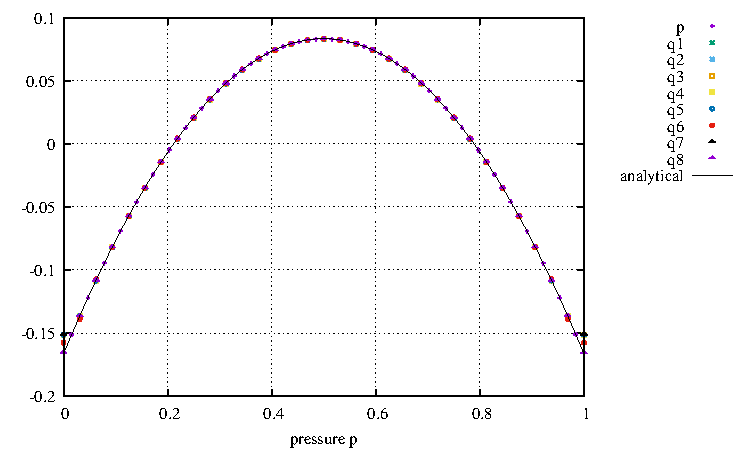
\includegraphics[width=10cm]{python_codes/fieldstone_01/results/pressure.pdf}\\
{\captionfont Pressure field}
\end{center}

\begin{center}
\includegraphics[width=15cm]{python_codes/fieldstone_01/results/solution.pdf}
\end{center}

One can also compute vertical/depth averages of the velocity, see Eq.~\eqref{eq:dhvelnorm}.
Note that the averages are computed somewhat naively: instead of computing integrals in the $x$-direction
at many depths I simply take an arithmetic average over rows of nodes. At high resolution the profiles
converge to the analytical profiles for the individual components and to the results 
obtained with \aspect. Please check \stone~110 for a better implementation.
\begin{center}
\includegraphics[width=10cm]{python_codes/fieldstone_01/results/vel_profile}\\
{\captionfont Vertical average of velocity. \aspect was run with the 'depth average' postprocessor
added to the prm file.}
\end{center}

\newpage
\subsection*{About the Fortran code}

I wrote the first ever version of this \stone in
Fortran90 around 2011. It is available in the {\foldernamefont simplefem} folder in this stone.
\index{general}{fortran90}

The code can be compiled as follows:
\begin{verbatim}
> gfortran -O3 linpack_d.f90 blas_routines.f simplefem.f90
\end{verbatim}
and run as follows:
\begin{verbatim}
> ./a.out 
\end{verbatim}
The solver used here does not make use of a sparse storage and relies on a dense matrix 
set of subroutine from BLAS and LinPACK\footnote{\url{https://en.wikipedia.org/wiki/LINPACK}}.
\begin{center}
\includegraphics[width=9cm]{python_codes/fieldstone_01/simplefem/timings/timings.pdf}\\
{\captionfont Despite a very naive application of the boundary conditions to the entire
assembled FE matrix, we find here that this part of the code is not taking long at all.}
\end{center}
There is no export of the results to ParaView format, only ascii text files.



\newpage
\subsection*{About the Julia code}

The python code was translated to julia in a rather straightforward manner. 
The matrix is still a full array (no sparse storage during the build process) 
and the boundary conditions
are applied naively. Even with a 80x80 resolution the memory use is under 2Gb. 
Note that there seems to be a limit as to the maximum size of the matrix array 
and for instance 96x96 yields to a crash.

In this version the matrix is stored as a full array. 
Before the linear system is solved, however, we must convert it to sparse storage:
\begin{verbatim}
Sps_amat=sparse(a_mat)
\end{verbatim}
When it comes to the solve, we have various options. The first and most 
simple one is similar to Matlab's backslash:
\begin{verbatim}
sol= Sps_amat\rhs
\end{verbatim}
Another possibility is cholesky\footnote{This method uses the CHOLMOD library from SuiteSparse:
\url{https://people.engr.tamu.edu/davis/suitesparse.html}} or ldlt or lu:
\begin{verbatim}
sol= cholesky(Sps_amat)\rhs
sol= ldlt(Sps_amat)\rhs
sol= lu(Sps_amat)\rhs
\end{verbatim}


The computed errors are of course identical to those of the python codes but we find that
at low resolutions the python code is much faster than the julia code: 
this is likely due to the time taken by julia to compile the code.
 

\begin{center}
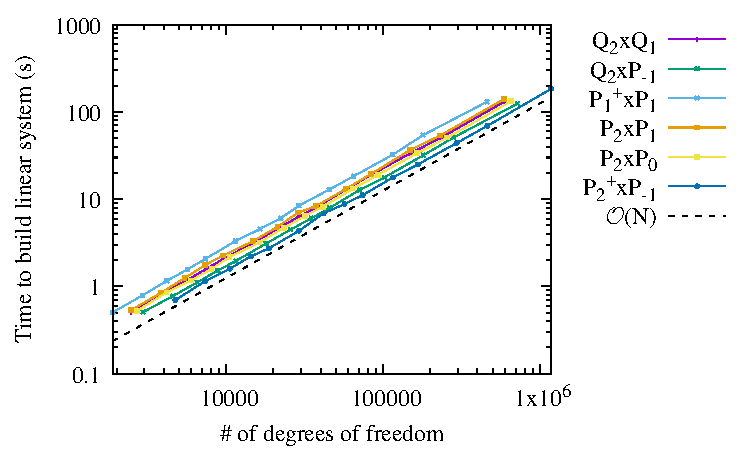
\includegraphics[width=5.7cm]{python_codes/fieldstone_01/results/julia/timings_build.pdf}
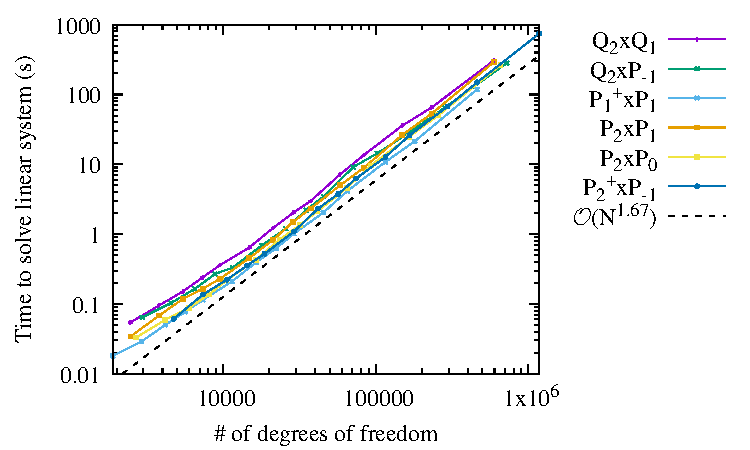
\includegraphics[width=5.7cm]{python_codes/fieldstone_01/results/julia/timings_solve.pdf}
\includegraphics[width=5.7cm]{python_codes/fieldstone_01/results/julia/errors.pdf}\\
{\captionfont Matrix building and solving times as obtained for nelx from 8 until 80, each 
resolution being run 10 times.}
\end{center}

We find that the LU-based solver is the fasted in this case.





 %%%%%%%%%%%%%%%%%%%%%%%%%%%%%%%%%%%%%%%%%%%%%%%%%%%%%%%%%%%

\chapter{Stokes sphere in 2D ($Q_1\times P_0$+penalty) \label{f02}} %%%%%%%%%%%%%%%%%%%%%%%%%%%%%%% 02
\lstinputlisting[language=bash,basicstyle=\small]{python_codes/fieldstone_02/keywords.ascii}

\begin{center}
Code at \url{https://github.com/cedrict/fieldstone/tree/master/python_codes/fieldstone_02}
\end{center}

\par\noindent\rule{\textwidth}{0.4pt}
%%%%%%%%%%%%%%%%%%%%%%%%%%%%%%%%%%%%%%%%%%%%%%%%%%%%%%%%%%%%%%%%%%%%%%%%%%%%%%%%%%%%%%%%%

This stone carries out the benchmark of Section~\ref{MMM-ss:stokes_sphere2D}
with $Q_1\times P_0$ elements using the penalty formulation.
The domain is a unit square and the fluid is characterised 
by $\rho=1$ and $\eta=1$ 
while the sphere is characterised 
by $\rho=1.01$ and $\eta=1000$.
The gravity vector is $\vec{g}=(0,-1)$. 

Boundary conditions are free slip on all sides ({\tt bc\_type=0}), 
no slip on all sides ({\tt bc\_type=1}) or free slip on the sides and bottom and open 
on top ({\tt bc\_type=2}).
Viscosity and density directly computed at the quadrature points.
The results are presented in Section~\ref{MMM-ss:stokes_sphere2D} and compared to 
those obtained with other codes.

Also, because of the inherent symmetry we can solve the system 
on only half the domain:
\begin{center}
\includegraphics[width=3cm]{python_codes/fieldstone_02/results/eta_1}
$\rightarrow$
\includegraphics[width=3cm]{python_codes/fieldstone_02/results/eta_2}
\end{center}


\begin{center}
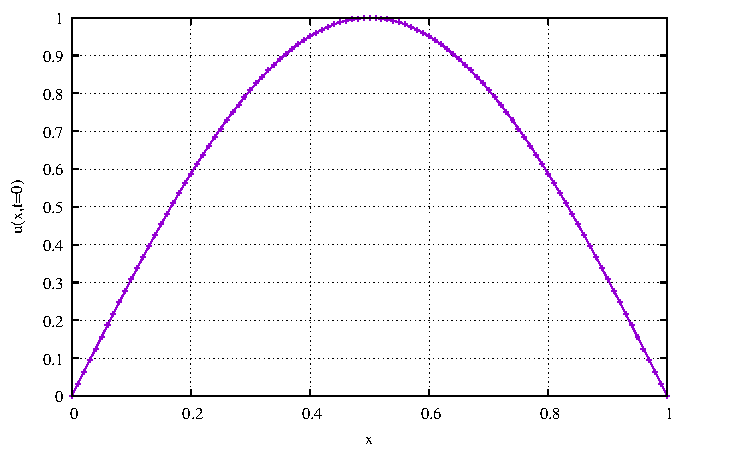
\includegraphics[width=3cm]{python_codes/fieldstone_02/results/u0}
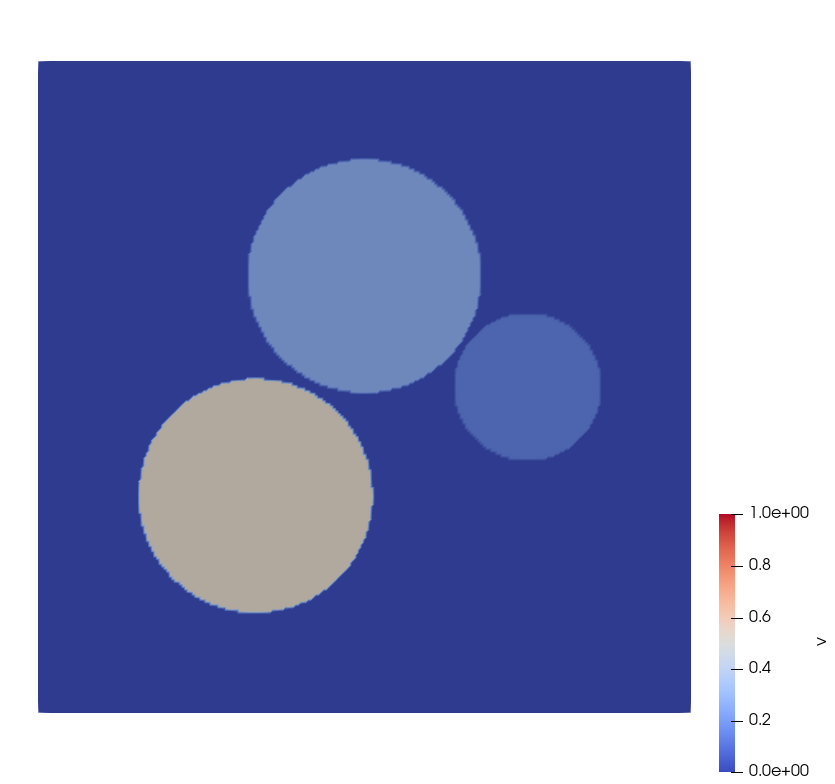
\includegraphics[width=3cm]{python_codes/fieldstone_02/results/v0}
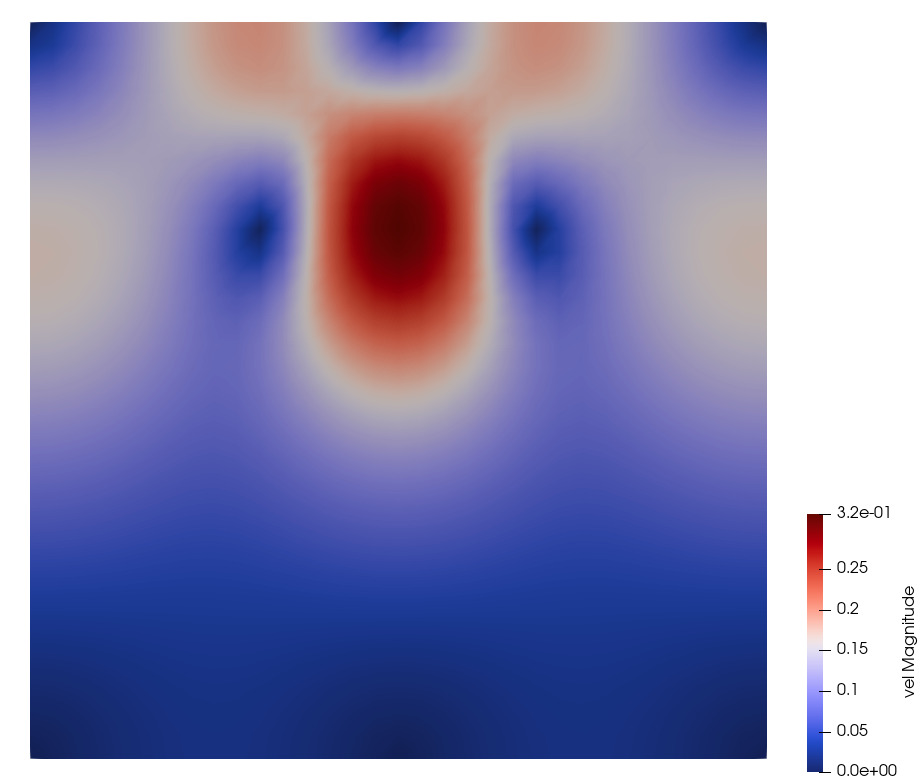
\includegraphics[width=3cm]{python_codes/fieldstone_02/results/vel0}
\includegraphics[width=3cm]{python_codes/fieldstone_02/results/sr0}
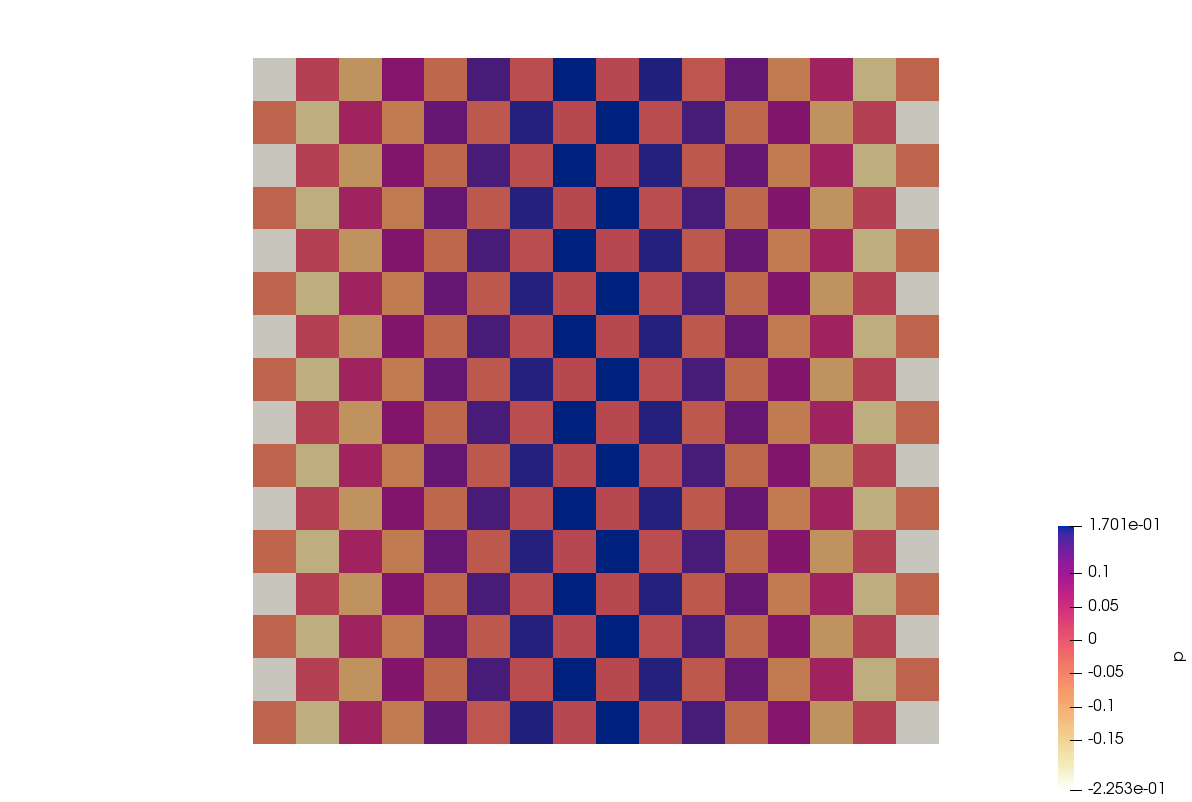
\includegraphics[width=3cm]{python_codes/fieldstone_02/results/p0}\\
\includegraphics[width=3cm]{python_codes/fieldstone_02/results/u1}
\includegraphics[width=3cm]{python_codes/fieldstone_02/results/v1}
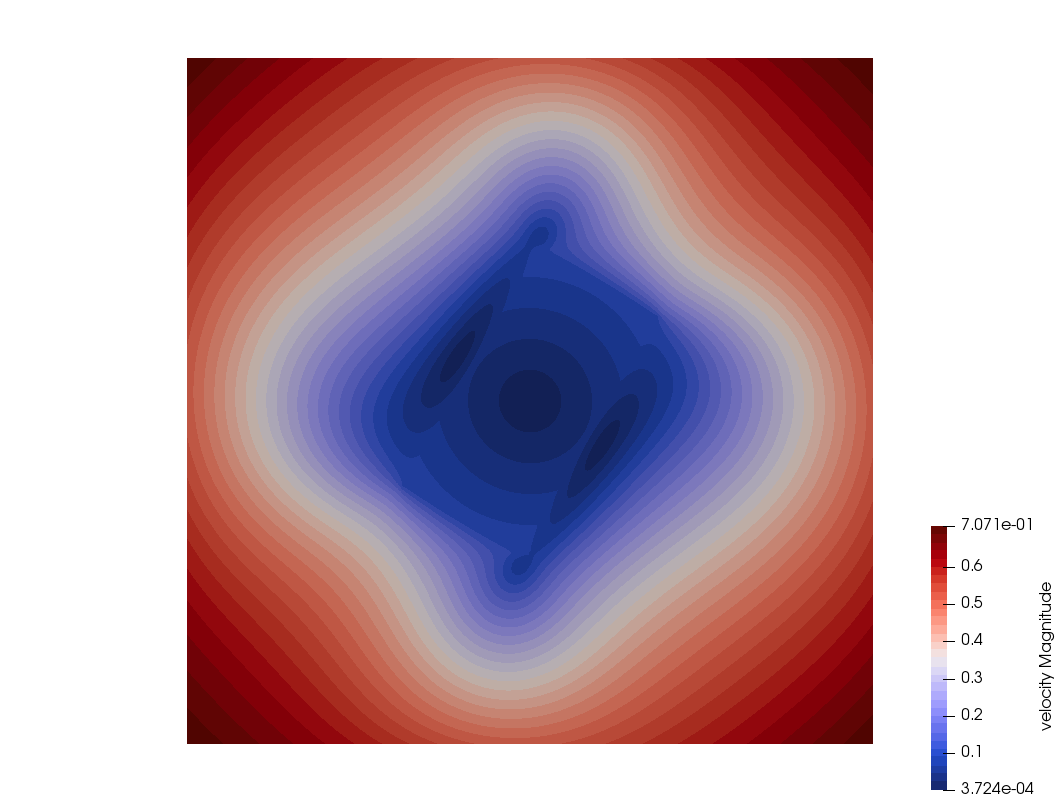
\includegraphics[width=3cm]{python_codes/fieldstone_02/results/vel1}
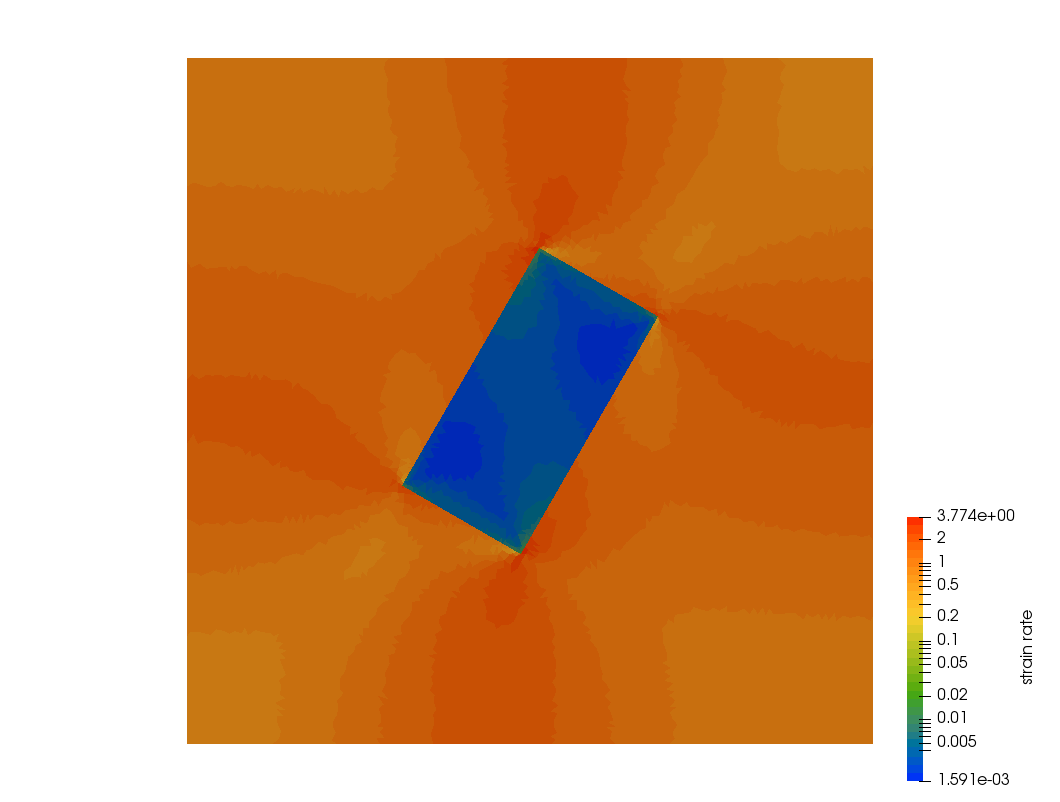
\includegraphics[width=3cm]{python_codes/fieldstone_02/results/sr1}
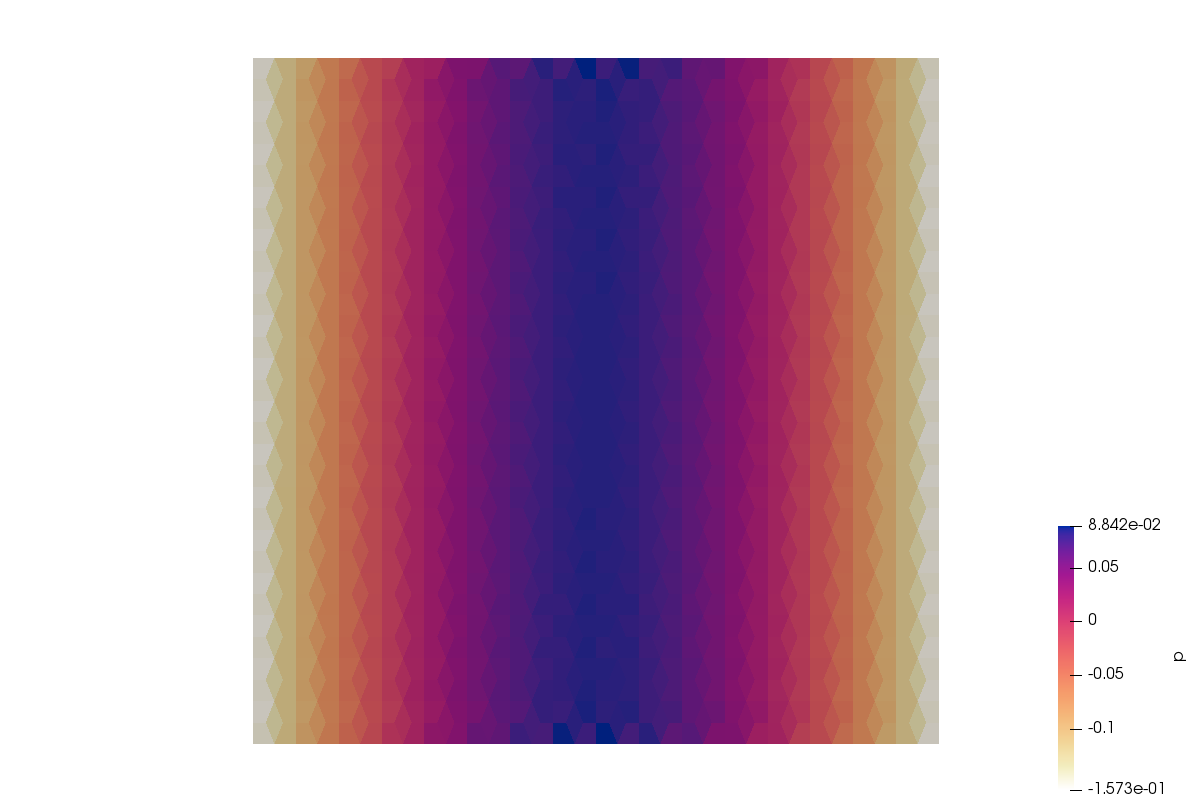
\includegraphics[width=3cm]{python_codes/fieldstone_02/results/p1}\\
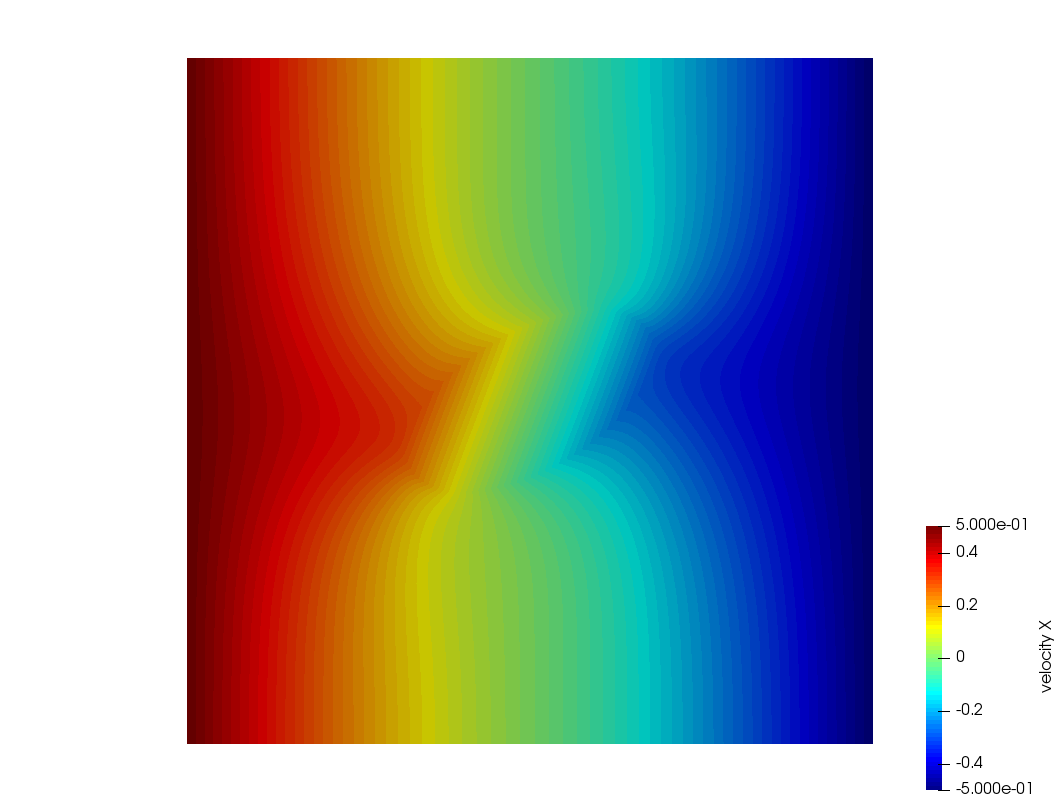
\includegraphics[width=3cm]{python_codes/fieldstone_02/results/u2}
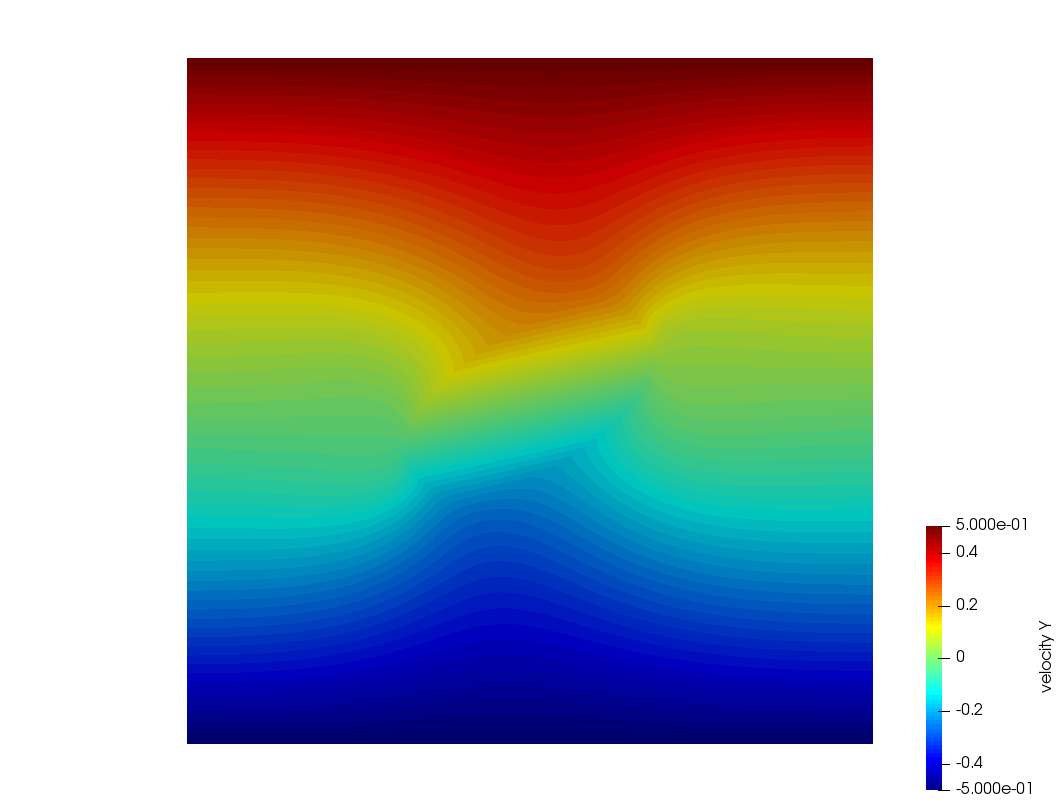
\includegraphics[width=3cm]{python_codes/fieldstone_02/results/v2}
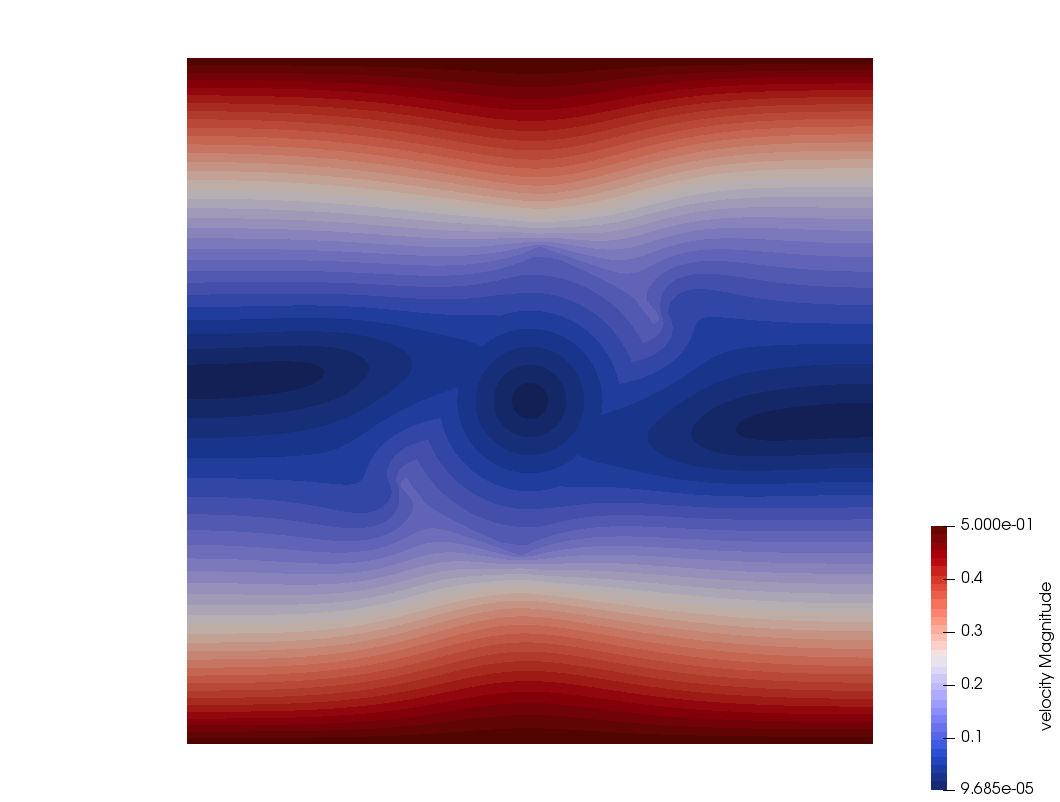
\includegraphics[width=3cm]{python_codes/fieldstone_02/results/vel2}
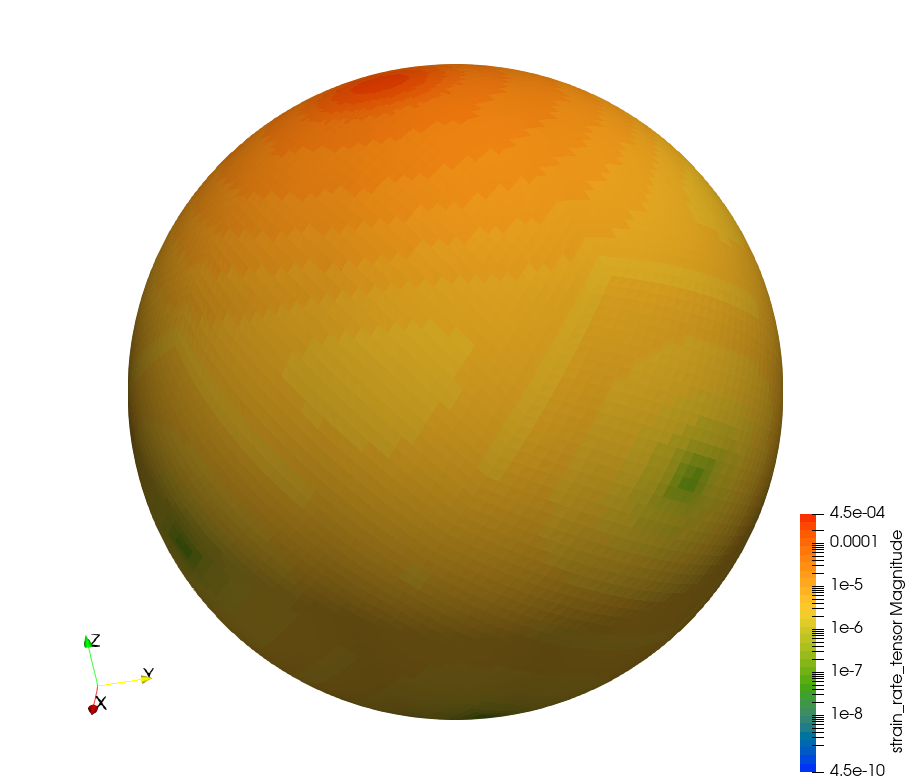
\includegraphics[width=3cm]{python_codes/fieldstone_02/results/sr2}
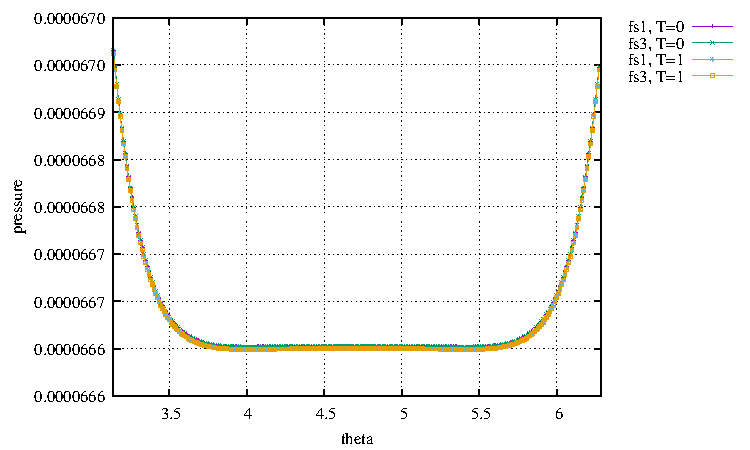
\includegraphics[width=3cm]{python_codes/fieldstone_02/results/p2}\\
{\captionfont Results on a $32\times 64$ grid. Top is free-slip, 
middle is no-slip, bottom is open top.}
\end{center}


 %%%%%%%%%%%%%%%%%%%%%%%%%%%%%%%%%%%%%%%%%%%%%%%%%%%%%%%%%%%

\chapter{Convection in a 2D box ($Q_1\times P_0$+penalty)\label{f03}} %%%%%%%%%%%%%%%%%%%%%%%%%%%%% 03

\includegraphics[height=1.25cm]{images/pictograms/FEM}

\includegraphics[height=1.25cm]{images/pictograms/replication}

\includegraphics[height=1.25cm]{images/pictograms/benchmark}
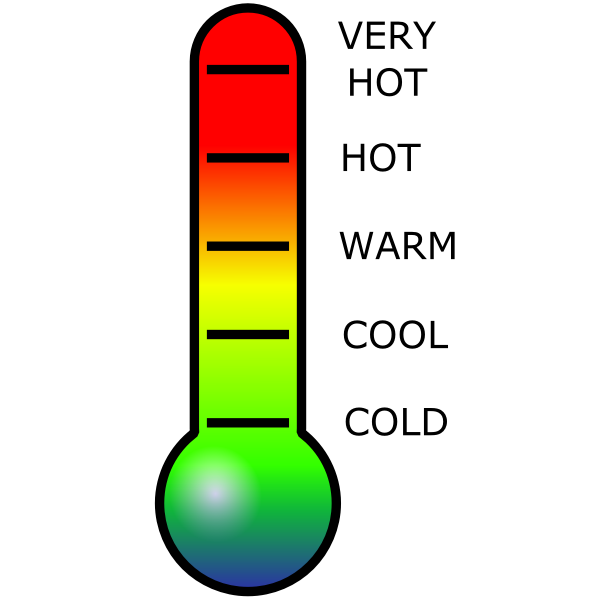
\includegraphics[height=1.25cm]{images/pictograms/temperature}

\lstinputlisting[language=bash,basicstyle=\small]{python_codes/fieldstone_03/keywords.ascii}

\begin{center}
\inpython
\injulia
{\small Codes: \url{https://github.com/cedrict/fieldstone/tree/master/python_codes/fieldstone_03}}
\end{center}

\par\noindent\rule{\textwidth}{0.4pt}

{\sl The julia stone was developed by Jort Jansen.}. \index{contributors}{J. Jansen}

\par\noindent\rule{\textwidth}{0.4pt}
%%%%%%%%%%%%%%%%%%%%%%%%%%%%%%%%%%%%%%%%%%%%%%%%%%%%%%%%%%%%%%%%%%%%%%%%%%%%%%%%%%%%%%%%%

\index{stopics}{$Q_1\times P_0$}

This benchmark deals with the 2-D thermal convection of a fluid 
of infinite Prandtl number in a rectangular closed cell.
In what follows, I carry out the case 1a, 1b, and 1c experiments as shown in 
Blankenbach \etal (1989) \cite{blbc89}:
steady convection with constant viscosity in a square box.

The temperature is fixed to zero on top and to $\Delta T$ at the bottom, 
with reflecting symmetry at the sidewalls (i.e. $\partial_x T=0$) 
and there are no internal heat sources. 
Free-slip conditions are implemented on all boundaries. 

The Rayleigh number is given by
\begin{equation}
\Ranb = \frac{\alpha g_y \Delta T h^3 }{\kappa \nu}
=\frac{\alpha g_y \Delta T h^3 \rho^2 C_p}{k \eta}
\end{equation}

In what follows, I use the following parameter values:  %, as given in \cite{krhb12}:
$L_x=L_y=1$,$\rho_0=c_P=k=\eta=1$, $T_0=0$, $\alpha=10^{-2}$, $g=10^{2}Ra$
and I run the model with $Ra=10^4,10^{5}$ and $10^6$.

The initial temperature field is given by 
\begin{equation}
T(x,y)=(1-y) - 0.01\cos(\pi x) \sin(\pi y)
\end{equation}
The perturbation in the initial temperature fields leads to 
a perturbation of the density field and sets the fluid in motion. 
Depending on the initial Rayleigh number, the system ultimately reaches a 
steady state after some time. 

The Nusselt number (i.e. the mean surface temperature gradient over mean bottom temperature)
is computed as follows \cite{blbc89}:
\begin{equation}
\Nunb = L_y \frac{\int_0^{L_x} \frac{\partial T}{\partial y}(y=L_y) \; dx  }{\int_0^{L_x} T(y=0) \; dx}
\label{eqNu}
\end{equation}
Note that in our case the denominator is equal to 1 since $L_x=1$ and the temperature at the 
bottom is prescribed to be 1.

If no convection is taking place (i.e. $\Ranb$ is too low) then only diffusion is taking place 
and the steady state temperature field is then $T(y)=1-y$, so that $\partial_y T=-1$ and 
we find that the Nusselt number is simply 1.

The steady state root mean square velocity and Nusselt number measurements
are indicated in the following Table alongside those of \cite{blbc89} and \cite{tack94}.
(Note that this benchmark was also carried out by many others (see Section~\ref{MMM-ss:blbc89}).

\begin{center}
\begin{tabular}{llccccc}
\hline
          &           & Blankenbach et al (1989) & Tackley (1994)  & 32x32 & 48x48 & 64x64  \\
\hline
\hline
$\Ranb=10^4$ & $V_{rms}$ &  $42.864947  \pm 0.000020$ & 42.775 & 42.89111& 42.87938& 42.87360\\  
          & $Nu$      &  $4.884409   \pm 0.000010$ & 4.878  & 4.783252 & 4.837800& 4.857373\\
$\Ranb=10^5$ & $V_{rms}$ &  $193.21454  \pm 0.00010 $ & 193.11 & 194.1032 & 193.6264 &  193.4519  \\ 
          & $Nu$      &  $10.534095  \pm 0.000010$ & 10.531 & 9.604454& 10.08087 &  10.26830  \\
$\Ranb=10^6$ & $V_{rms}$ &  $833.98977  \pm 0.00020 $ & 833.55 & & & \\
          & $Nu$      &  $21.972465  \pm 0.000020$ & 21.998 & & & \\
\hline
\end{tabular}\\
{\small Steady state Nusselt number $Nu$ and $\upnu_{rms}$ measurements as reported in the literature. }
\end{center}

Food for thought: Looking at the mass, momentum and energy conservation equations, 
we see that that they are coupled: the temperature enters the rhs of the momentum 
equation since the density depends on the temperature (Boussinesq approximation)
while the velocity is present in the advection term of the energy equation.
One should then solve all three equations with $u,v,p,T$ as unknowns. However
this is rarely done in practice and often the system is solved in a segregated way:
first solve for $u,v,p$ assuming $T$ known, then solving for $T$ assuming $u,v,p$ known.
If small time steps are used this is a reasonable approach, or, like in this case, when 
one wishes to compute the steady state of the system rather than an accurate time-evolution
of the system. Better schemes are available and one example thereof is explained in Kronbichler et al (2012) 
\cite{krhb12}.

Also, the current version of this \stone uses a Crank-Nicolson approach for the 
time discretisation of the $\partial T/\partial t$ term as explained in Section~\ref{MMM-sec:timediscr}.

Something must be said about how the Nusselt number is computed. 
Its calculation requires the integral of the temperature gradient along an edge. 
Because it is much simpler to compute the temperature gradient in the middle of the 
element alongside other quantities such as pressure, this (elemental) quantity is 
used in the Nusselt number calculations, which makes it inaccurate and therefore 
explains the discrepancy between the computed values and those of other publications.
Check the Consistent Boundary Flux method in Section~\ref{MMM-ss:cbf}.

Finally, it is expected that the thickness of the 
boundary layers decreases with higher Rayleigh number values.
As a consequence, in order to appropriately capture those, one needs 
a higher resolution than at low $\Ranb$ numbers. This explains why 
acceptable results are obtained for $\Ranb=10^4$  even at low resolution $32\times 32$.

Note that the results obtained with \aspect at comparable resolution ought to be 
more accurate since \aspect relies on quadratic elements for both velocity and 
temperature. 

A few remarks about the code. It relies on $Q_1\times P_0$ elements with a penalty
formulation so that the pressure degrees of freedom are not taken into account. 
The temperature is also bi-linear ($Q_1$) so that the temperature and velocity nodes 
are identical and no distinction is made between them.

Steady state has been reached when the relative velocity and temperature difference between two consecutive 
time steps is less than a tolerance set to $10^{-6}$. 


\newpage
\paragraph{Results for $\Ranb=10^4$}.
\begin{center}
\includegraphics[width=16cm]{python_codes/fieldstone_03/results_1e4/64x64/solution.pdf}\\
\includegraphics[width=5cm]{python_codes/fieldstone_03/results_1e4/Tavrg.pdf}
\includegraphics[width=5cm]{python_codes/fieldstone_03/results_1e4/vrms.pdf}\\
\includegraphics[width=5cm]{python_codes/fieldstone_03/results_1e4/Nu.pdf}
\includegraphics[width=5cm]{python_codes/fieldstone_03/results_1e4/Nu_vrms.pdf}
\includegraphics[width=5cm]{python_codes/fieldstone_03/results_1e4/convergence.pdf}\\
{\captionfont Note that the \aspect data have been shifted so that the location of the 
first vrms peak coincides with the one of the 64x64 run.}
\end{center}

\newpage
\paragraph{Results for $\Ranb=10^5$}.
\begin{center}
\includegraphics[width=16cm]{python_codes/fieldstone_03/results_1e5/64x64/solution.pdf}\\
\includegraphics[width=5cm]{python_codes/fieldstone_03/results_1e5/Tavrg.pdf}
\includegraphics[width=5cm]{python_codes/fieldstone_03/results_1e5/vrms.pdf}\\
\includegraphics[width=5cm]{python_codes/fieldstone_03/results_1e5/Nu.pdf}
\includegraphics[width=5cm]{python_codes/fieldstone_03/results_1e5/Nu_vrms.pdf}\\
\includegraphics[width=5cm]{python_codes/fieldstone_03/results_1e5/convergence.pdf}\\
\end{center}

\newpage
\paragraph{Results for $\Ranb=10^6$}.
\begin{center}
\includegraphics[width=16cm]{python_codes/fieldstone_03/results_1e6/48x48/solution.pdf}\\
\includegraphics[width=5cm]{python_codes/fieldstone_03/results_1e6/Tavrg.pdf}
\includegraphics[width=5cm]{python_codes/fieldstone_03/results_1e6/vrms.pdf}\\
\includegraphics[width=5cm]{python_codes/fieldstone_03/results_1e6/Nu.pdf}
\includegraphics[width=5cm]{python_codes/fieldstone_03/results_1e6/Nu_vrms.pdf}
\end{center}


I have tested the influence of the CFL number (0.5 instead of 1) and it does not change much at all.





 %%%%%%%%%%%%%%%%%%%%%%%%%%%%%%%%%%%%%%%%%%%%%%%%%%%%%%%%%%%

\chapter{The lid driven cavity ($Q_1\times P_0$+penalty) \label{f04}} %%%%%%%%%%%%%%%%%%%%%%%%%%%%% 04

\includegraphics[height=1.25cm]{images/pictograms/replication}

\includegraphics[height=1.25cm]{images/pictograms/benchmark}
\includegraphics[height=1.25cm]{images/pictograms/FEM}

%%%%%%%%%%%%%%%%%%%%%%%%%%%%%%%%%%%%%%%%%%%%%%%%%%%%%%%%%%%%%%%%%%%%%%%%%%%%%%%%%%%%%%%%%%%%%%%%%%%

\lstinputlisting[language=bash,basicstyle=\small]{python_codes/fieldstone_04/keywords.ascii}

\begin{center}
\inpython
{\small Code: \url{https://github.com/cedrict/fieldstone/tree/master/python_codes/fieldstone_04}}
\end{center}

\par\noindent\rule{\textwidth}{0.4pt}
%%%%%%%%%%%%%%%%%%%%%%%%%%%%%%%%%%%%%%%%%%%%%%%%%%%%%%%%%%%%%%%%%%%%%%%%%%%%%%%%%%%%%%%%%
\index{stopics}{$Q_1\times P_0$}

The lid driven cavity is a famous Computational Fluid Dynamics test case 
\cite{kawa61,ghgs82,paac67,bope98,brsa06,grdn97,shde00}
and has been studied in countless publications with a wealth of numerical techniques
(see \cite{ertu09} for a succinct review) and also in the laboratory \cite{kost84}.

It models a plane flow of an isothermal isoviscous fluid in a rectangular (usually square) lid-driven cavity. 
The boundary conditions are no slip on left, right and bottom. The gravity is set to zero as the flow
is entirely driven by the moving lid.

%---------------------------------------------------------
\subsection*{The lid driven cavity problem ({\tt ldc=0})}
In the standard case, the upper side of the cavity moves in its own plane at unit speed, while the other sides are fixed.
This thereby introduces a discontinuity in the boundary conditions at the two upper corners of the cavity and yields
an uncertainty as to which boundary (side or top) the corner points belong to. 
In this version of the code the top corner nodes are considered to be part of the lid. If these are excluded 
the recovered pressure showcases an extremely large checkboard pattern.

This benchmark is usually dicussed in the context of low to very high Reynolds number with the full 
Navier-Stokes equations being solved (with the noticeable exception of \cite{sagl81a,sagl81b,chpc95,eid2005}
which focus on the Stokes equation). 
In the case of the incompressible Stokes flow, 
the absence of inertia renders this problem instantaneous so that only one time step/Stokes solve is needed.

%---------------------------------------------------------
\subsection*{The lid driven cavity problem - regularisation I ({\tt ldc=1})}

We avoid the top corner nodes issue altogether by  
prescribing the horizontal velocity of the lid as follows: 
\begin{equation}
u(x)=16x^2(1-x)^2.
\end{equation}
In this case the velocity and its first derivative is continuous at the corners. This is the so-called regularised lid-driven cavity problem \cite{piva94}. The factor 16 ensures that $\max\limits_{[0,1]}(u)=1$.
 
%---------------------------------------------------------
\subsection*{The lid driven cavity problem - regularisation II ({\tt ldc=2})}

Another regularisation was presented in de Frutos \etal \cite{dejn16} and 
also in Appendix D.4 of \textcite{john16} (2016). 
Here, a regularized lid driven cavity is studied which is consistent in the sense that 
${\bm \nabla}\cdot{\bm v}=0$ 
holds also at the corners of the domain.
There are no-slip conditions at the boundaries $x=0$, $x=1$, and $y=0$. 

The velocity at $y=1$ is given by

\begin{eqnarray}
u(x) &=& 1-\frac{1}{4}\left( 1-\cos (\frac{x_1-x}{x_1}\pi)  \right)^2   \quad\quad x\in[0,x_1] \nonumber\\
u(x) &=& 1 \quad\quad x\in[x_1,1-x_1] \nonumber\\
u(x) &=& 1-\frac{1}{4}\left( 1-\cos (\frac{x-(1-x_1)}{x_1}\pi)  \right)^2   \quad\quad x\in[1-x_1,1]
\end{eqnarray}
Results are obtained with $x_1=0.1$.


A 100$\times$100 element grid is used. 
A zero vertical velocity is prescribed at the top and the exact form of the 
prescribed horizontal velocity is controlled by the {\tt ldc} parameter.

\begin{center}
\includegraphics[width=7cm]{python_codes/fieldstone_04/results/p.pdf}
\includegraphics[width=7cm]{python_codes/fieldstone_04/results/q.pdf}\\
{\captionfont Left: pressure $p$ at $y=L_y$; Right: smoothed pressure $q$ at $y=L_y$.}
\end{center}

\begin{center}
\includegraphics[width=12cm]{python_codes/fieldstone_04/results/velocities}\\
\includegraphics[width=12cm]{python_codes/fieldstone_04/results/pressures}\\
\includegraphics[width=12cm]{python_codes/fieldstone_04/results/strainrates}
\end{center}

 %%%%%%%%%%%%%%%%%%%%%%%%%%%%%%%%%%%%%%%%%%%%%%%%%%%%%%%%%%%

\chapter{SolCx benchmark ($Q_1\times P_0$+penalty)\label{f05}} %%%%%%%%%%%%%%%%%%%%%%%%%%%%%%%%%%%% 05
\noindent
\includegraphics[height=1.25cm]{images/pictograms/replication}
\includegraphics[height=1.25cm]{images/pictograms/benchmark}
\includegraphics[height=1.25cm]{images/pictograms/FEM}
\includegraphics[height=1.25cm]{images/pictograms/paraview}

%%%%%%%%%%%%%%%%%%%%%%%%%%%%%%%%%%%%%%%%%%%%%%%%%%%%%%%%%%%%%%%%%%%%%%%%%%%%%%%%%%%%%%%%%%%%%%%%%%%

%\lstinputlisting[language=bash,basicstyle=\small]{python_codes/fieldstone_05/keywords.ascii}

\begin{center}
\inpython
\infortran
{\small Codes: \url{https://github.com/cedrict/fieldstone/tree/master/python_codes/fieldstone_05}}
\end{center}

\par\noindent\rule{\textwidth}{0.4pt}

Last revision: Oct. 28th, 2024.

\par\noindent\rule{\textwidth}{0.4pt}

%%%%%%%%%%%%%%%%%%%%%%%%%%%%%%%%%%%%%%%%%%%%%%%%%%%%%%%%%%%%%%%%%%%%%%%%%%%%%%%%%%%%%%%%%

The experiment is fully described in Section~\ref{MMM-ss:solcx}.
The viscosity is prescribed at the quadrature points 
If the number of elements is even in the $x$-direction direction, all elements 
(and their associated quadrature points)
have a constant viscosity ($1$ or  $10^6$). If it is odd, then the elements situated 
at the viscosity jump have half their integration points with $\eta=1$ and half 
with $\eta=10^6$ 
(which is a pathological case since the used quadrature rule inside elements cannot represent 
accurately such a jump).  

\begin{center}
\includegraphics[width=8cm]{python_codes/fieldstone_05/results/errors_even.pdf}
\includegraphics[width=8cm]{python_codes/fieldstone_05/results/errors_odd.pdf}\\
{\captionfont Velocity and pressure error convergence as a function of mesh size and for various values
of the penalty parameter. Left: even number of elements in each direction; Right: odd numbers.
}
\end{center}

Because of the high viscosity in the right part of the domain, the penalty parameter should 
be high enough to insure an incompressible flow and thereby recover the expected convergence rate
(at least for the even case). Note that values higher than $\lambda=10^{10}$ yield erroneous solutions 
due to round-off errors. 

\begin{center}
\includegraphics[width=6.5cm]{python_codes/fieldstone_05/results/rho}
\includegraphics[width=6.5cm]{python_codes/fieldstone_05/results/eta}\\
\includegraphics[width=4cm]{python_codes/fieldstone_05/results/vel}
\includegraphics[width=4cm]{python_codes/fieldstone_05/results/vel_error}
\includegraphics[width=4cm]{python_codes/fieldstone_05/results/press}
\includegraphics[width=4cm]{python_codes/fieldstone_05/results/press_error}\\
\includegraphics[width=4cm]{python_codes/fieldstone_05/results/exx}
\includegraphics[width=4cm]{python_codes/fieldstone_05/results/eyy}
\includegraphics[width=4cm]{python_codes/fieldstone_05/results/exy}
\includegraphics[width=4cm]{python_codes/fieldstone_05/results/sr}\\
{\captionfont Results obtained on $100 \times 100$ mesh for $\lambda=10^{10}$.}
\end{center}



\infortran
Note that a Fortran90 version of this code is available in the same folder. \index{general}{fortran90}


 %%%%%%%%%%%%%%%%%%%%%%%%%%%%%%%%%%%%%%%%%%%%%%%%%%%%%%%%%%%

\chapter{SolKz benchmark ($Q_1\times P_0$+penalty)\label{f06}} %%%%%%%%%%%%%%%%%%%%%%%%%%%%%%%%%%%% 06

\includegraphics[height=1.5cm]{images/pictograms/benchmark}

\lstinputlisting[language=bash,basicstyle=\small]{python_codes/fieldstone_06/keywords.ascii}

\begin{center}
Code at \url{https://github.com/cedrict/fieldstone/tree/master/python_codes/fieldstone_06}
\end{center}

\par\noindent\rule{\textwidth}{0.4pt}
%%%%%%%%%%%%%%%%%%%%%%%%%%%%%%%%%%%%%%%%%%%%%%%%%%%%%%%%%%%%%%%%%%%%%%%%%%%%%%%%%%%%%%%%%

The SolKz benchmark \cite{repa87} is similar to the SolCx benchmark.
but the viscosity is now a function of the space coordinates: 
\begin{equation}
\eta(y)=\exp(By) \quad {\rm with} \quad B=13.8155
\end{equation}
It is however not a discontinuous function but grows exponentially with the vertical coordinate so that its overall variation is again $10^6$. 
The forcing is again chosen by imposing a spatially variable density variation as follows:
\begin{equation}
\rho(x,y)=\sin(2y) \cos(3\pi x)
\end{equation}
Free slip boundary conditions are imposed on all sides of the domain.
This benchmark is presented in Zhong (1996) \cite{zhon96} as well and is studied 
in Duretz \etal (2011) \cite{dumg11} and Gerya \etal (2013) \cite{gemd13}.

\begin{center}
\includegraphics[width=14cm]{python_codes/fieldstone_06/results/solution.pdf}
\end{center}

\begin{center}
\includegraphics[width=10cm]{python_codes/fieldstone_06/results/errors.pdf}\\
{\captionfont Velocity and pressure error as a function of mesh size.}
\end{center}
 %%%%%%%%%%%%%%%%%%%%%%%%%%%%%%%%%%%%%%%%%%%%%%%%%%%%%%%%%%%

\chapter{SolVi benchmark ($Q_1\times P_0$+penalty) \label{f07}} %%%%%%%%%%%%%%%%%%%%%%%%%%%%%%%%%%% 07

\includegraphics[height=1.5cm]{images/pictograms/benchmark}

\lstinputlisting[language=bash,basicstyle=\small]{python_codes/fieldstone_07/keywords.ascii}

\begin{center}
Code at \url{https://github.com/cedrict/fieldstone/tree/master/python_codes/fieldstone_07}
\end{center}

\par\noindent\rule{\textwidth}{0.4pt}
%%%%%%%%%%%%%%%%%%%%%%%%%%%%%%%%%%%%%%%%%%%%%%%%%%%%%%%%%%%%%%%%%%%%%%%%%%%%%%%%%%%%%%%%%

Following SolCx and SolKz, the SolVi inclusion benchmark solves 
a problem with a discontinuous viscosity field, but in this case 
the viscosity field is chosen in such a way that the discontinuity 
is along a circle. Given the regular nature of the grid used by a majority of codes and the present one, 
this ensures that the discontinuity in the viscosity never aligns to cell boundaries.
This in turns leads to almost discontinuous pressures along the interface which are difficult to represent accurately.
Schmid \& Podlachikov (2003) \cite{scpo03} derived a simple analytic solution for the pressure and 
velocity fields for a circular 
inclusion under simple shear and it was used in \cite{deka08,sunh10,dumg11,krhb12,gemd13}.

Because of the symmetry of the problem, we only have to solve over the top right quarter of the domain.
The analytical solution requires a strain rate boundary condition (e.g., pure shear) to be applied far away 
from the inclusion. In order to avoid using very large domains and/or dealing with this type of boundary condition 
altogether, the analytical solution is evaluated and imposed on the boundaries of the domain. 
By doing so, the truncation error introduced while discretizing the strain rate boundary condition is removed.

A characteristic of the analytic solution is that the pressure is zero inside the inclusion, while outside it follows the relation
\begin{equation}
p_m = 4 \dot{\epsilon}
\frac{\eta_m(\eta_i-\eta_m)}{\eta_i+\eta_m}
\frac{r_i^2}{r^2} \cos(2\theta)
\end{equation}
where $\eta_i = 10^3$ is the viscosity of the inclusion 
and $\eta_m = 1$ is the viscosity of the background media, $\theta=\tan^{-1}(y/x)$,
and $\dot{\epsilon}=1$ is the applied strain rate.

Deubelbeiss \& Kauss (2008) \cite{deka08} thoroughly investigated this problem with various 
numerical methods (FEM, FDM), with and without tracers, 
and conclusively showed how various averagings lead to different results. 
Duretz et al (2011) \cite{dumg11} obtained a first order convergence for both pressure and velocity, 
while Kronbichler et al (2012) \cite{krhb12}
and Gerya et al (2013) \cite{gemd13} showed that the use of adaptive mesh refinement in respectively the FEM and FDM 
yields convergence rates which depend on refinement strategies. 

\begin{center}
\includegraphics[width=8cm]{python_codes/fieldstone_07/results/errors}\\
{\captionfont Velocity and pressure error convergence as a function of mesh size.}
\end{center}

\includegraphics[width=15cm]{python_codes/fieldstone_07/results/solution}

\begin{center}
\includegraphics[width=7cm]{python_codes/fieldstone_07/results/pressbottom}
\includegraphics[width=7cm]{python_codes/fieldstone_07/results/veldiag}\\
{\captionfont Left: Pressure at the bottom of the domain. Right: $u$ on the diagonal $x=y$.}
\end{center}

 %%%%%%%%%%%%%%%%%%%%%%%%%%%%%%%%%%%%%%%%%%%%%%%%%%%%%%%%%%%

\chapter{The indentor benchmark ($Q_1\times P_0$+penalty)\label{f08}} %%%%%%%%%%%%%%%%%%%%%%%%%%%%% 08

\includegraphics[height=1.5cm]{images/pictograms/benchmark}

\lstinputlisting[language=bash,basicstyle=\small]{python_codes/fieldstone_08/keywords.ascii}

\begin{center}
Code at \url{https://github.com/cedrict/fieldstone/tree/master/python_codes/fieldstone_08}
\end{center}

\par\noindent\rule{\textwidth}{0.4pt}
%%%%%%%%%%%%%%%%%%%%%%%%%%%%%%%%%%%%%%%%%%%%%%%%%%%%%%%%%%%%%%%%%%%%%%%%%%%%%%%%%%%%%%%%%

The punch benchmark is one of the few boundary value problems involving plastic solids for which there exists an exact solution. 
Such solutions are usually either for highly simplified geometries (spherical or axial symmetry, for instance) or simplified material models (such as rigid plastic solids) \cite{kacha04}.

In this experiment, a rigid punch indents a rigid plastic half space; the slip line field theory gives 
exact solutions as shown in section~\ref{MMM-sec:punch}. 
The plane strain formulation of the equations and the detailed solution to the problem were derived in the Appendix of \cite{thfb08} and are also presented in \cite{gepd98}.

The two dimensional punch problem has been extensively studied numerically for the past 40 years 
\cite{zihl75,zihp95,chpe01,chan99,huhy99,yuti06,bufs08,raab07} and has been used to draw a parallel 
with the tectonics of eastern China in the context of the 
India-Eurasia collision \cite{tamo76,mota77}.
It is also worth noting that it has been carried out in one form or another in series of 
analogue modelling articles 
concerning the same region, with a rigid indenter colliding with a rheologically stratified 
lithosphere \cite{peta88,daco88,jodc90}.
 
Numerically, the one-time step punch experiment is performed on a two-dimensional
domain of purely plastic von Mises material. 
Given that the von Mises rheology yield criterion does not depend on pressure
(see Section~\ref{MMM-sec:vMcriterion}), the density of the material and/or the gravity 
vector is set to zero. Sides are set to free slip boundary conditions, the bottom to no slip, 
while a vertical velocity $(0,-v_p)$ is prescribed at the top boundary for nodes 
whose $x$ coordinate is within $[L_x/2-\delta/2,L_x/2+\delta/2]$. 

The following parameters are used: $L_x=1$, $L_y=0.5$, $\mu_{min}=10^{-3}$, 
$\mu_{max}=10^3$, $v_p=1$, $\delta=0.11111$ 
and the yield value of the material is set to $\sigma_Y=1$. 

The analytical solution predicts that the angle of the shear bands stemming from the sides of the punch 
is $\pi/4$, that the pressure right under the punch is $1+\pi$, 
and that the velocity of the rigid blocks on each side of the punch is $v_p/\sqrt{2}$ 
(this is simply explained by invoking conservation of mass).

In what follows I show results of the rough and smooth punch for a 124x68 grid. The difference between the two
lies in the nature of the kinematic boundary conditions under the punched area. 'rough' means that the indentor 
also fixes the horizontal velocity component to zero while it is free in the smooth case.

We see that the smooth punch does not trigger the checkerboard pressure modes as much as the rough case 
and we recover nicely the analytical pressure under the punch \cite{thfb08,gltf18}.

\newpage
%................................................................................
\paragraph{Rough punch} 

\begin{center}
\includegraphics[width=6cm]{python_codes/fieldstone_08/results/rough/velocity.pdf}
\includegraphics[width=6cm]{python_codes/fieldstone_08/results/rough/pressure.pdf}\\
\includegraphics[width=6cm]{python_codes/fieldstone_08/results/rough/strainrate.pdf}
\includegraphics[width=6cm]{python_codes/fieldstone_08/results/rough/stress.pdf}\\
\includegraphics[width=6cm]{python_codes/fieldstone_08/results/rough/u_stats.pdf}
\includegraphics[width=6cm]{python_codes/fieldstone_08/results/rough/v_stats.pdf}\\
\includegraphics[width=6cm]{python_codes/fieldstone_08/results/rough/residual.pdf}
\includegraphics[width=6cm]{python_codes/fieldstone_08/results/rough/diff_uv.pdf}\\
{\captionfont a,b,c,d) velocity, pressure, strainrate and stress at the top of the domain; 
e,f) min/max value of $u$ and $v$;
g,h) residual and normalised velocity difference.}
\end{center}

\newpage
\includegraphics[width=16cm]{python_codes/fieldstone_08/results/rough/solution.pdf}


%................................................................................
\newpage
\paragraph{Smooth punch}

\begin{center}
\includegraphics[width=6cm]{python_codes/fieldstone_08/results/smooth/velocity.pdf}
\includegraphics[width=6cm]{python_codes/fieldstone_08/results/smooth/pressure.pdf}\\
\includegraphics[width=6cm]{python_codes/fieldstone_08/results/smooth/strainrate.pdf}
\includegraphics[width=6cm]{python_codes/fieldstone_08/results/smooth/stress.pdf}\\
\includegraphics[width=6cm]{python_codes/fieldstone_08/results/smooth/u_stats.pdf}
\includegraphics[width=6cm]{python_codes/fieldstone_08/results/smooth/v_stats.pdf}\\
\includegraphics[width=6cm]{python_codes/fieldstone_08/results/smooth/residual.pdf}
\includegraphics[width=6cm]{python_codes/fieldstone_08/results/smooth/diff_uv.pdf}\\
{\captionfont a,b,c,d) velocity, pressure, strainrate and stress at the top of the domain; 
e,f) min/max value of $u$ and $v$;
g,h) residual and normalised velocity difference.}
\end{center}

\newpage
\includegraphics[width=16cm]{python_codes/fieldstone_08/results/smooth/solution.pdf}




 %%%%%%%%%%%%%%%%%%%%%%%%%%%%%%%%%%%%%%%%%%%%%%%%%%%%%%%%%%%
 
\chapter{The annulus benchmark ($Q_1\times P_0$+penalty) \label{f09}} %%%%%%%%%%%%%%%%%%%%%%%%%%%%% 09
\includegraphics[height=1.25cm]{images/pictograms/benchmark}
\includegraphics[height=1.25cm]{images/pictograms/FEM}

%%%%%%%%%%%%%%%%%%%%%%%%%%%%%%%%%%%%%%%%%%%%%%%%%%%%%%%%%%%%%%%%%%%%%%%%%%%%%%%%%%%%%%%%%%%%%%%%%%%

\lstinputlisting[language=bash,basicstyle=\small]{python_codes/fieldstone_09/keywords.ascii}

\begin{center}
\inpython
{\small Code: \url{https://github.com/cedrict/fieldstone/tree/master/python_codes/fieldstone_09}}
\end{center}

\par\noindent\rule{\textwidth}{0.4pt}

{\sl This fieldstone was developed in collaboration with Prof. E.G.P. Puckett}. 
\index{contributors}{E.G.P. Puckett}

\par\noindent\rule{\textwidth}{0.4pt}
%%%%%%%%%%%%%%%%%%%%%%%%%%%%%%%%%%%%%%%%%%%%%%%%%%%%%%%%%%%%%%%%%%%%%%%%%%%%%%%%%%%%%%%%%%%%

The benchmark is described fully in Section~\ref{MMM-ss:anconv} in which 
an analytical solution to the isoviscous incompressible Stokes equations 
is derived in an annulus geometry.
The velocity and pressure fields are as follows:

\begin{eqnarray}
v_r(r,\theta)     &=&  g(r) k \sin(k\theta), \\
v_\theta(r,\theta)&=&  f(r) \cos(k \theta), \\ 
p(r,\theta)       &=&  k h(r) \sin(k \theta), \\
\rho (r,\theta)   &=& \aleph(r) k \sin (k \theta), 
\end{eqnarray}
with $f(r)$, $g(r)$, $h(r)$ given in Section~\ref{MMM-ss:anconv}.
The parameters $A$ and $B$ are chosen so that $v_r(R_1)=v_r(R_2)=0$, i.e.
the velocity is tangential to both inner and outer surfaces.
The gravity vector is radial and of unit length.
In the present case, we set $R_1=1$, $R_2=2$ and $C=-1$.
The parameter $k$ can take values 0,1,2,3,... 

\begin{center}
\includegraphics[width=5cm]{python_codes/fieldstone_09/velocity}
\includegraphics[width=5cm]{python_codes/fieldstone_09/vr}
\includegraphics[width=5cm]{python_codes/fieldstone_09/vtheta}\\
{\small Left to right: velocity norm, $r$ component, $\theta$ component}
\end{center}

\begin{center}
\includegraphics[width=7cm]{python_codes/fieldstone_09/density}
\includegraphics[width=7cm]{python_codes/fieldstone_09/pressure}\\
{\small Left: density field; right: pressure field.}
\end{center}

\begin{center}
\includegraphics[width=7cm]{python_codes/fieldstone_09/psi}
\includegraphics[width=7cm]{python_codes/fieldstone_09/psi_arrows}\\
{\small Left: $\psi$ field; right: $\psi$ isolines with velocity arrows.}
\end{center}

\includegraphics[width=15cm]{python_codes/fieldstone_09/errors}

 %%%%%%%%%%%%%%%%%%%%%%%%%%%%%%%%%%%%%%%%%%%%%%%%%%%%%%%%%%%

\chapter{Stokes sphere in 3D ($Q_1 \times P_0$+penalty)\label{f10}} %%%%%%%%%%%%%%%%%%%%%%%%%%%%%%%% 10
\includegraphics[height=1.25cm]{images/pictograms/FEM}
\includegraphics[height=1.25cm]{images/pictograms/3d}

%%%%%%%%%%%%%%%%%%%%%%%%%%%%%%%%%%%%%%%%%%%%%%%%%%%%%%%%%%%%%%%%%%%%%%%%%%%%%%%%%%%%%%%%%

\lstinputlisting[language=bash,basicstyle=\small]{python_codes/fieldstone_10/keywords.key}

\begin{center}
\inpython
\injulia
\infortran
{\small Code: \url{https://github.com/cedrict/fieldstone/tree/master/python_codes/fieldstone_10}}
\end{center}

\par\noindent\rule{\textwidth}{0.4pt}
%%%%%%%%%%%%%%%%%%%%%%%%%%%%%%%%%%%%%%%%%%%%%%%%%%%%%%%%%%%%%%%%%%%%%%%%%%%%%%%%%%%%%%%%%

Last revision: Sept. 27th, 2024.

\par\noindent\rule{\textwidth}{0.4pt}
%%%%%%%%%%%%%%%%%%%%%%%%%%%%%%%%%%%%%%%%%%%%%%%%%%%%%%%%%%%%%%%%%%%%%%%%%%%%%%%%%%%%%%%%%


%----------------------------------------------------------
\subsection*{Manufactured solution ({\tt experiment=5})}

It is described in Section~\ref{MMM-ss:mms3Dgen}.
The velocity and pressure fields are:
\begin{eqnarray}
u(x,y,z) &=& x(1-x)(1-2y)(1-2z)\\
v(x,y,z) &=& (1-2x) y(1-y) (1-2z) \\
w(x,y,z) &=& -2(1-2x)(1-2y)z(1-z) \\
p(x,y,z) &=& (2x-1)(2y-1)(2z-1)
\end{eqnarray}
This flow field has the built-in property that there is no flux through the 
boundaries, i.e. the normal component of the velocity field is zero on each face. 

\begin{center}
\includegraphics[width=5.6cm]{python_codes/fieldstone_10/results/exp5/press}
\includegraphics[width=5.6cm]{python_codes/fieldstone_10/results/exp5/vel}
\end{center}

\begin{center}
\includegraphics[width=5.6cm]{python_codes/fieldstone_10/results/exp5/vrms}
\includegraphics[width=5.6cm]{python_codes/fieldstone_10/results/exp5/conv}
\includegraphics[width=5.6cm]{python_codes/fieldstone_10/results/exp5/p_stats}
\end{center}
We recover the expected second order velocity error convergence 
and first order pressure error convergence. 
Surprisingly, we find that the results are not sensitive to the value of the penalty parameter $\lambda$.

This \stone is implemented in both python and julia, in order to look at
performance aspects. Both versions of the code are as close to each other 
as possible. The FE build and solve times are recorded and we find
that the build time grows linearly with the number of elements in the python 
case but not in the julia case. I suspected that the sparse storage of julia
(as opposed to a linked list converted to sparse matrix in python) makes it slow
so I ran the code without the assembly and indeed it is then linear with the 
number of elements.
I need to find a better way!!

\begin{center}
\includegraphics[width=8cm]{python_codes/fieldstone_10/results/exp5/julia/build.pdf}
\includegraphics[width=8cm]{python_codes/fieldstone_10/results/exp5/julia/solve.pdf}\\
{\captionfont Matrix building and system solve times for both python and julia codes.
Obtained with penalty=1e6. Each resolution is run 3 times.}
\end{center}


%----------------------------------------------------------
\subsection*{Aquarium ({\tt experiment=0})}

FS on all sides, $\rho=\eta=g_z=1$, $\lambda=10^6$

\begin{center}
\includegraphics[width=5.7cm]{python_codes/fieldstone_10/results/exp0/stats_uv}
\includegraphics[width=5.7cm]{python_codes/fieldstone_10/results/exp0/stats_w}
\includegraphics[width=5.7cm]{python_codes/fieldstone_10/results/exp0/stats_p}\\
{\captionfont Statistics of $u,v,w,p$.}
\end{center}

We expect a zero velocity field. This is the case (down to machine precision) for the $u$
and $v$ components, but since the penalty method yields a weakly compressible flow, 
the vertical component $w$ is larger but remains small.
The pressure is expected to be lithostatic and it should be -0.5 at the top and +0.5 at 
the bottom. Pressure statistics seem to converge towards these values. 





%------------------------------
\subsection*{Stokes sphere}

The domain is a unit cube. Free slip boundary conditions 
are imposed on all sides. The mesh counts 
nelx*nely*nelz=nel elements and 
nnx*nny*nnz=NV nodes.
The density and the viscosity are prescribed in the domain 
by means of two functions:
the density is set to $1+\delta \rho$ inside a sphere of radius 0.123456789 centered 
at (0.5,0.5,0.5) and 1 outside. The viscosity is 1000 inside the sphere
and 1 outside.  The gravity vector is set to $\vec{g}=(0,0,-1)$.
This is the benchmark presented in Section~\ref{MMM-ss:stokes_sphere_3D}.

The FE matrix size grows even faster now than in the previous 2D case so
choosing the right matrix storage is of paramount importance. 

Three experiments are carried out:
\begin{enumerate}
\item[Exp.~1:] the one described above.
Free slip or no slip boundary conditions.
We see that the pressure field is dominated by the lithostatic signal.
\item[Exp.~2:] same as experiment 1, but a reference density of 1 is substracted to all densities, so that 
the sphere density is 1 and the density of the surrounding fluid is now 0. In essence, we remove a
'background' density which does not participate in the flow generation, and thereby get rid of the 
lithostatic signal of the pressure.
Free slip or no slip boundary conditions.
\item[Exp.~3:] same as experiment 2, but the top boundary is now open (free surface)
\end{enumerate} 

\begin{center}
\includegraphics[width=5.7cm]{python_codes/fieldstone_10/results/exp1/grid}
\includegraphics[width=5.7cm]{python_codes/fieldstone_10/results/exp1/vel}
\includegraphics[width=5.7cm]{python_codes/fieldstone_10/results/exp1/press}\\
\includegraphics[width=5.7cm]{python_codes/fieldstone_10/results/exp1/visc}
\includegraphics[width=5.7cm]{python_codes/fieldstone_10/results/exp1/dens}\\
{\small Exp.~1: resolution $24\times 24\times 24$}
\end{center}

\begin{center}
\includegraphics[width=7cm]{python_codes/fieldstone_10/results/exp2/dens_2}
\includegraphics[width=7cm]{python_codes/fieldstone_10/results/exp2/press_2}\\
{\small Exp.~2: Density and pressure fields. Resolution 24x24x24}
\end{center}


\begin{center}
\includegraphics[width=7cm]{python_codes/fieldstone_10/results/exp3/press_3}
\includegraphics[width=7cm]{python_codes/fieldstone_10/results/exp3/vel_3}\\
{\small Exp.~3: pressure and velocity fields. Resolution 24x24x24}
\end{center}

\begin{center}
\includegraphics[width=5.6cm]{python_codes/fieldstone_10/results/exp1/pressure.pdf}
\includegraphics[width=5.6cm]{python_codes/fieldstone_10/results/exp2/pressure.pdf}
\includegraphics[width=5.6cm]{python_codes/fieldstone_10/results/exp3/pressure.pdf}\\
{\captionfont Elemental pressure for all elements as a function of their vertical 
(middle) coordinate for (from left to right) experiments 1, 2 and 3. }
\end{center}

Note that a similar fortran code is present in the folder. 

If the option 'quarter' is true, then the model takes advantage of the symmetries 
of the problem and runs it in a quarter of the original domain, so that 
the domain is then $0.5\times 0.5 \times 1$. Measurements/results are identical 
to the full cube ones, but at a much lower cost.

\begin{center}
\includegraphics[width=4cm]{python_codes/fieldstone_10/results/quarter_FS/press}
\includegraphics[width=4cm]{python_codes/fieldstone_10/results/quarter_FS/sr}
\includegraphics[width=4cm]{python_codes/fieldstone_10/results/quarter_FS/vel}
\includegraphics[width=4cm]{python_codes/fieldstone_10/results/quarter_FS/eta}\\
{\captionfont Resolution $32\times 32\times 64$ - FS}
\end{center}


\begin{center}
\includegraphics[width=7cm]{images/stokes_sphere3D/vrms_FS}
\includegraphics[width=7cm]{images/stokes_sphere3D/vrms_NS}\\
{\captionfont Left: FS; Right: NS. Results obtained with this stones and other ones, as well as ASPECT.
See Section~\ref{MMM-ss:stokes_sphere_3D} for all results.}
\end{center}

\newpage
%%%%%%%%%%%%%%%%%%%%%%%%%%%%%%%%%%%%%%%%%%%%%%%%%%%%%%%%
\section*{Trying $Q_2\times Q_0$+penalty... because why not}

Based on a discussion with A. Regorda I have coded a $Q_2\times Q_0$
(still with penalty) version of the \stone: {\tt stoneQ2Q0.py}.
The following results are obtained with {\tt script\_Q2Q0}.

I first naively used a 1 point integration (as for the 
$Q_1 \times P_0$ element) only for the 
penalty term, only to realise that the penalty term $\K_\lambda$ should be 
under-integrated, but not necessarily using a single point. 

This sparked the study on the influence of the quadrature rule 
of the penalty term on the accuracy of results.

I also implemented the consistent pressure recovery described 
in Section~\ref{MMM-ss:cpr}.
This results in a nodal pressure field (which I call $q$) which is 
solution of 
\[
{\bm M} \cdot \vec{Q} = \vec{f}
\]
where ${\bm M}$ is the $Q_2$ mass matrix that 
is integrated with the same quadrature as the viscous block $\K_\eta$
but the rhs $\vec{f}$ is integrated with the same quadrature as 
the penalty block $\K_\lambda$.
In the end I also keep the pressure $p$ computed in the middle of the element
using $p= \lambda \vec\nabla\cdot \vec\upnu$.

Finally to save time I have used the fact that the Jacobian of the 
coordinate change for cuboids is a diagonal matrix containing terms $h_x/2$,
$h_y/2$, $h_z/2$ on the diagonal. This means that this can be computed once
and for all for all elements. 

%----------------------------------------------------------
\subsection*{Aquarium ({\tt experiment=0})}

Fress slip on all sides, $\rho=\eta=g_z=1$, $\lambda=10^6$

\begin{center}
\includegraphics[width=5.7cm]{python_codes/fieldstone_10/resultsQ2/exp0/errv}
\includegraphics[width=5.7cm]{python_codes/fieldstone_10/resultsQ2/exp0/errp}
\includegraphics[width=5.7cm]{python_codes/fieldstone_10/resultsQ2/exp0/errq}\\
\includegraphics[width=8cm]{python_codes/fieldstone_10/resultsQ2/exp0/p_stats}
\end{center}

We expect a zero velocity field. This is the case (down to machine precision) 
for the $u$ and $v$ components, but since the penalty method yields a 
weakly compressible flow, the vertical component $w$ is much larger 
then $u$ and $v$.
The pressure is expected to be lithostatic and it should be -0.5 at the top 
and +0.5 at the bottom. Pressure statistics to converge towards these values. 

\begin{center}
\includegraphics[width=5cm]{python_codes/fieldstone_10/resultsQ2/exp0/press}
\includegraphics[width=5cm]{python_codes/fieldstone_10/resultsQ2/exp0/w}\\
{\captionfont $w$ and $p$ for resolution $20\times 20 \times 20$.}
\end{center}

Note that at resolution 20x20x20 build time is 10min, and solve time is 48 min!
Given this 'performance' this will limit a lot the tests we can carry out...

%----------------------------------------------------------
\subsection*{Manufactured solution ({\tt experiment=5})}

See Section~\ref{MMM-ss:mms3Dgen} for the analytical expressions 
of the velocity, pressure and body force vector.

\begin{center}
\includegraphics[width=5.7cm]{python_codes/fieldstone_10/resultsQ2/exp5/errv}
\includegraphics[width=5.7cm]{python_codes/fieldstone_10/resultsQ2/exp5/errp}
\includegraphics[width=5.7cm]{python_codes/fieldstone_10/resultsQ2/exp5/errq}\\
\includegraphics[width=8cm]{python_codes/fieldstone_10/resultsQ2/exp5/vrms}
\includegraphics[width=8cm]{python_codes/fieldstone_10/resultsQ2/exp5/p_stats}
\end{center}

Since the analytical solution of this experiment is quadratic then the 
velocity basis functions can exactly represent the solution inside each
element and the accuracy of the velocity solution depends on the penalty parameter and
not on resolution.
We clearly see that using only one integration point for the penalty term results
in lesser accurate velocities.
Interestingly we obtain a superconvergence (third order) of the $q$ error 
for a 2x2x2 quadrature and only a linear convergence for the $q$ error
for a 3x3x3 quadrature.
The pressure $q$ obtained with only 1 quad point yields results that are so off
that they do not show on the plots.
Finally we note that we obtain pressures that often exceed the analytical 
bounds for min and max pressure except for $q$ with 2x2x2 quadrature.
This seems to indicate that a 2x2x2 quadrature is preferable.
We keep investigating in the next section with a more suitable manufactured
solution benchmark.

\begin{center}
\includegraphics[width=5.7cm]{python_codes/fieldstone_10/resultsQ2/exp5/vel}
\includegraphics[width=5.7cm]{python_codes/fieldstone_10/resultsQ2/exp5/p}
\includegraphics[width=5.7cm]{python_codes/fieldstone_10/resultsQ2/exp5/q}\\
{\captionfont $||\vec\upnu||$, $p$ and $q$ for resolution $20\times 20 \times 20$.}
\end{center}

%----------------------------------------------------------
\subsection*{Manufactured solution ({\tt experiment=6})}

After the observations made about the previous experiment we then turn to 
another 3D manufactured solution as described in Section~\ref{MMM-ss:mms3Dgen}.

\begin{eqnarray}
f(x) &=& x^2(1-x)^2 \\
g(y) &=& y^2(1-y)^2 \\
h(z) &=& z^2(1-z)^2 \\
u(x,y,z) &=& fg'h' \\
v(x,y,z) &=& f'gh'  \\
w(x,y,z) &=& -2f'g'h \\
p(x,y,z) &=& -f'g'h'
\end{eqnarray}


\begin{center}
\includegraphics[width=5.7cm]{python_codes/fieldstone_10/resultsQ2/exp6/errv}
\includegraphics[width=5.7cm]{python_codes/fieldstone_10/resultsQ2/exp6/errp}
\includegraphics[width=5.7cm]{python_codes/fieldstone_10/resultsQ2/exp6/errq}\\
\includegraphics[width=5.7cm]{python_codes/fieldstone_10/resultsQ2/exp6/vrms}
\includegraphics[width=5.7cm]{python_codes/fieldstone_10/resultsQ2/exp6/p_stats}
\includegraphics[width=5.7cm]{python_codes/fieldstone_10/resultsQ2/exp6/q_stats}
\end{center}

We find that:
\begin{itemize}
\item The velocity error exhibits cubic convergence {\it only} 
for $2\times 2\times 2$ quadrature and is the smallest.
\item the convergence of the $p$ pressure is puzzling
\item the convergence of the $q$ pressure is second order (!) for 
$2\times 2\times 2$ quadrature and is also the smallest.   
\end{itemize}

The conclusion is clear: {\color{violet}the penalty term $\K_\lambda$ 
must be integrated with $2\times 2\times 2$ quadrature}.

TODO: determine analytical min max of pressure

 %%%%%%%%%%%%%%%%%%%%%%%%%%%%%%%%%%%%%%%%%%%%%%%%%%%%%%%%%%%

\chapter{Stokes sphere in 3D ($Q_1\times P_0$ - mixed) \label{f11}} %%%%%%%%%%%%%%%%%%%%%%%%%%%%%%% 11
\includegraphics[height=1.25cm]{images/pictograms/FEM}
\includegraphics[height=1.25cm]{images/pictograms/3d}
\includegraphics[height=1.25cm]{images/pictograms/paraview}

%%%%%%%%%%%%%%%%%%%%%%%%%%%%%%%%%%%%%%%%%%%%%%%%%%%%%%%%%%%%%%%%%%%%%%%%%%%%%%%%%%%%%%%%%%%%%%%%%%%

%\lstinputlisting[language=bash,basicstyle=\small]{python_codes/fieldstone_11/keywords.ascii}

\begin{center}
\inpython
{\small Code: \url{https://github.com/cedrict/fieldstone/tree/master/python_codes/fieldstone_11}}
\end{center}

\par\noindent\rule{\textwidth}{0.4pt}

Last revision: August 30th, 2025.

\par\noindent\rule{\textwidth}{0.4pt}

%%%%%%%%%%%%%%%%%%%%%%%%%%%%%%%%%%%%%%%%%%%%%%%%%%%%%%%%%%%%%%%%

The setup is identical to the one of the \stone~\ref{f10}.

The difference lies in how we solve the Stokes equation. This stone does not rely on 
the penalty method (Section \ref{MMM-sec:penalty}) 
but instead used a mixed formulation, i.e. we solve for both 
velocity and pressure at the same time (see Section~\ref{MMM-sec:mixed}).

In the case when free slip boundary conditions are applied on all 
6 faces of the cube we know that there is a pressure nullspace, i.e.
that the pressure can only be computed up to a constant. In order to 
remove this nullspace one must add an additional constraint 
We here choose to (somewhat arbitrarily) enforce that the average pressure 
over the whole domain is zero:
\[
<p>=\frac{1}{|\Omega|} \int_\Omega p \; dV =0 
\]
Since the code relies of discontinuous zero-th order polynomial shape functions 
for pressure this condition simply writes (and since $|\Omega|=1$):
\[
<p>=\frac{1}{|\Omega|} \int_\Omega p\;  dV 
=  \sum_{e} \int_{\Omega_e} p dV = \sum_e p_e V_e = h^3 \sum_e p_e =0
\]
Dividing all by $h^3$, the condition becomes simply:
\[
p_1 + p_2 + p_3 + ... + p_{nel} = 0
\]
How this constraint is incorporated in the Stokes matrix is explained in Section~\ref{MMM-ss_pnorm}.

It is also important to remember that if one now switches to a free surface at the top then 
the null space is absent from the equations and the constraint should be removed/switched off.

The pressure normalisation is controled by the boolean {\sl pnormalise} in the code. 
Since the pressure constraint adds a line to the global FE, we then logically have:
\begin{lstlisting}
if pnormalise:
   a_mat = np.zeros((Nfem+1,Nfem+1),dtype=np.float64) 
   rhs   = np.zeros(Nfem+1,dtype=np.float64)    
else:
   a_mat = np.zeros((Nfem,Nfem),dtype=np.float64)
   rhs   = np.zeros(Nfem,dtype=np.float64)       
\end{lstlisting} 
Once the solve has been done, we retrieve the separate velocity and pressure fields as follows:
\begin{lstlisting}
u,v,w=np.reshape(sol[0:NfemV],(nnp,3)).T
p=sol[NfemV:Nfem]
\end{lstlisting} 
and the Lagrange multiplier is a scalar at the bottom of the array:
\begin{lstlisting}
if pnormalise:
   print("     -> Lagrange multiplier: %.4es" % sol[Nfem])
\end{lstlisting} 

It is quite easy in python to visualise the matrix structure 
with the spy function:
\begin{lstlisting}
plt.spy(a_mat)
\end{lstlisting} 
and we see that we indeed recover
the block structure with a zero block for the pressure-pressure entries.  
\begin{center}
\includegraphics[width=8cm]{python_codes/fieldstone_11/results/matrix6x6x6.pdf}
\includegraphics[width=8cm]{python_codes/fieldstone_11/results/matrix16x16x16.pdf}\\
{\captionfont Sparsity pattern of the Stokes matrix for a 6x6x6 mesh (left) and a 16x16x16 mesh (right).}
\end{center}

\begin{center}
\includegraphics[width=5.7cm]{python_codes/fieldstone_11/results/vel}
\includegraphics[width=5.7cm]{python_codes/fieldstone_11/results/press}
\includegraphics[width=5.7cm]{python_codes/fieldstone_11/results/sr}\\
{\captionfont Velocity, pressure and effective strain rate fields for a $20\times 20\times 20$ mesh.}
\end{center}


\underline{Remark}: the matrix building in this \stone is rather naive. The 
$\K$ and $\G$ matrices are built as full matrices and later assembled
in {\python a\_mat} which is also a full matrix, only to be converted 
to CSR format before calling the solver. 
In subsequent stones I usually only build {\python a\_mat} in {\python lil\_matrix} format.


 
 %%%%%%%%%%%%%%%%%%%%%%%%%%%%%%%%%%%%%%%%%%%%%%%%%%%%%%%%%%%

\chapter{consistent pressure recovery ($Q_1\times P_0$+penalty)\label{f12}} %%%%%%%%%%%%%%%%%%%%%%% 12
\includegraphics[height=1.25cm]{images/pictograms/benchmark}
\includegraphics[height=1.25cm]{images/pictograms/FEM}

%%%%%%%%%%%%%%%%%%%%%%%%%%%%%%%%%%%%%%%%%%%%%%%%%%%%%%%%%%%%%%%%%%%%%%%%%%%%%%%%%%%%%%%%%%%%%%%%%%%

\lstinputlisting[language=bash,basicstyle=\small]{python_codes/fieldstone_12/keywords.ascii}

\begin{center}
\inpython
{\small Code: \url{https://github.com/cedrict/fieldstone/tree/master/python_codes/fieldstone_12}}
\end{center}

\par\noindent\rule{\textwidth}{0.4pt}
%%%%%%%%%%%%%%%%%%%%%%%%%%%%%%%%%%%%%%%%%%%%%%%%%%%%%%%%%%%%%%%%%%%%%%%%%%%%%%%%%%%%%%%%%%%%%%

We start from the analytical benchmark of Section \ref{MMM-mms1} and we use $Q_1 \times P_0$
elements with a penalty formulation. 
We have seen in \stone~\ref{f01} how to recover the elemental pressure as a postprocessing step. 
However, the discontinous nature of the pressure field (and the presence of a
parasitic checkerboard mode) can be problematic for many reasons 
(pressure enters the rheology, equation of state, plotting, ...). 
We then wish to project the elemental pressure onto the nodes of the mesh while at the same 
time filtering the checkerboard mode out. 

Terminology: in general, when a discontinuous elemental pressure is used in a stone, 
it is called $p$ while its projection onto the velocity nodes is called $q$. 
In this case we compute several nodal pressures as explained in Section~\ref{MMM-psmoothing}:

\begin{itemize}
%...........
\item $q_1$: smoothed pressure obtained with the  center-to-node approach (scheme 1).

\item $q_2$: the nodal pressure obtained by smoothing the elemental pressure using element areas (scheme 2).

\item $q_3$: the nodal pressure obtained by smoothing the elemental p using triangle areas (scheme 3).

\item $q_4$: smoothed pressure obtained with the center-to-node approach with inverse element area weighing.

\item $q_5$: is not computed because same as 6.

\item $q_6$: consistent pressure recovery through FE (scheme 5 \& 6)

\item $q_7$: consistent pressure recovery with lumped mass matrix. 

\item $q_8$: bilinear interpolation. 

\end{itemize}

Since the setups showcase Dirichlet boundary conditions on all four sides, 
the pressure solution is normalised so that $\int p\; dV =0 $.

\begin{remark}
Nodes on edges and corners may need special treatment as documented in Sani et al \cite{sagl81a} or
Lee et al (1979) \cite{legs79} which is not done here.  
Nodes on the boundary showcase the largest errors. Maybe then use CBF instead for these?
\end{remark}

\begin{remark}
Lee et al (1979) \cite{legs79} discuss two different ways to compute the lumped mass matrix. 
\end{remark}

\begin{remark}
In the same folder there is a fortran90 version of the consistent recovery algorithm.
\end{remark}

I have created a simple checkerboard filter. Let $\phi=\pm 1$ denote this field.
The filter is applied as follows:
\[
p_{filtered} = p - \left( \frac{1}{|\Omega|} \iint_\Omega p \phi dV \right) \phi
\]
It is in fact a a projection. If $p=\alpha \phi$  where $\alpha$ is a scalar, then 
it is trivial to show that $p_{filtered} =0$.
Likewise, if $p=constant$ then $p_{filtered}=p$.
This idea is probably to be found in the relevant publications of Section~\ref{MMM-psmoothing}
in some form or shape. 

There is much more work to be done on this topic/stone! Look at cost vs accuracy!

\newpage
%...............................................
%...............................................
\paragraph{Regular mesh made of square elements}

We compute the error convergence for $p$, $q_i$ $(i=1,...8)$:
\begin{center}
\includegraphics[width=10cm]{python_codes/fieldstone_12/results/reg/errors}
\end{center}
The elemental pressure error converges like $h^1$, $q_{1-7}$ converge like $h^{1.5}$ and 
$q^8$ converges like $h^2$.


\begin{center}
\includegraphics[width=5.3cm]{python_codes/fieldstone_12/results/reg/pressure}
\includegraphics[width=5.3cm]{python_codes/fieldstone_12/results/reg/p_error}
\includegraphics[width=5.3cm]{python_codes/fieldstone_12/results/reg/q1_error}\\
\includegraphics[width=5.3cm]{python_codes/fieldstone_12/results/reg/q2_error}
\includegraphics[width=5.3cm]{python_codes/fieldstone_12/results/reg/q3_error}
\includegraphics[width=5.3cm]{python_codes/fieldstone_12/results/reg/q4_error}\\
\includegraphics[width=5.3cm]{python_codes/fieldstone_12/results/reg/q6_error}
\includegraphics[width=5.3cm]{python_codes/fieldstone_12/results/reg/q7_error}
\includegraphics[width=5.3cm]{python_codes/fieldstone_12/results/reg/q8_error}\\
{\captionfont Left: pressure fields as a function of the $x$-coordinate. 
Right: absolute error with regards to the analytical solution. All on 32x32 mesh.}
\end{center}

It is worth noticing that the checkerboard is (visually) not present:
\begin{center}
\includegraphics[width=4.5cm]{python_codes/fieldstone_12/results/reg/p32}
\includegraphics[width=4.5cm]{python_codes/fieldstone_12/results/reg/p48}
\includegraphics[width=4.5cm]{python_codes/fieldstone_12/results/reg/p64}\\
{\captionfont Elemental pressure field for 32x32, 48x48 and 64x64 resolutions.}
\end{center}
This means that the algorithms above fulfill an interpolation function, but not a smoothing one.

\newpage
%............................................
\paragraph{Adding randomness to internal node positions} We now add a random value $\xi h$ to the 
location of all nodes which are not on the boundary where $h$=$L_x$/nelx and we set $\xi=20\%$.
In this case a 32x32 mesh looks as follows:

\begin{center}
\includegraphics[width=7cm]{python_codes/fieldstone_12/results/rand/area_0p1}
\includegraphics[width=7cm]{python_codes/fieldstone_12/results/rand/area_0p2}\\
{\captionfont Mesh 32x32 elements. Left: $\xi=0.1$; Right: $\xi=0.2$}
\end{center}

We repeat the same exercise as before on such a mesh and look at the errors

\begin{center}
\includegraphics[width=8cm]{python_codes/fieldstone_12/results/rand/errors_nofilter}
\includegraphics[width=8cm]{python_codes/fieldstone_12/results/rand/errors_filter}\\
{\captionfont Velocity and pressure errors for $\xi=0.2$. Left: no filter, right: with filter.} 
\end{center}

It is easy to see the drastic effect that the filter has on the min/max of the elemental pressure:
\begin{center}
\includegraphics[width=7cm]{python_codes/fieldstone_12/results/rand/rawp_nofilter}
\includegraphics[width=7cm]{python_codes/fieldstone_12/results/rand/rawp_filter}\\
{\captionfont min/max value of elemental pressure field: Left: no filter, right: with filter}
\end{center}

Rather surprisingly we find that $q_1$ still proves to be the most accurate of all pressures and it converges
with $h^{1.5}$(?) as before. Because checkerboard modes are triggered the convergence of the elemental 
pressure is more chaotic but on average linear. 
The $q_6$ and $q_7$ fields seem to unexpectedly stop converging above a given resolution, which 
probably comes from the lack of adequate treatment of sides and corners.
All others converge with $h^{1.5}$ and $q_4$ seems a bit more chaotic than the others.
Scheme 8 seems to be the best here again but with an erratic convergence about $h^{1.5}$

\begin{center}
\includegraphics[width=5cm]{python_codes/fieldstone_12/results/rand/pressure}
\includegraphics[width=5cm]{python_codes/fieldstone_12/results/rand/p_error}
\includegraphics[width=5cm]{python_codes/fieldstone_12/results/rand/q1_error}\\
\includegraphics[width=5cm]{python_codes/fieldstone_12/results/rand/q2_error}
\includegraphics[width=5cm]{python_codes/fieldstone_12/results/rand/q3_error}
\includegraphics[width=5cm]{python_codes/fieldstone_12/results/rand/q4_error}\\
\includegraphics[width=5cm]{python_codes/fieldstone_12/results/rand/q6_error}
\includegraphics[width=5cm]{python_codes/fieldstone_12/results/rand/q7_error}
\includegraphics[width=5cm]{python_codes/fieldstone_12/results/rand/q8_error}\\
{\captionfont all obtained in 32x32 mesh}
\end{center}

\begin{center}
\includegraphics[width=5cm]{python_codes/fieldstone_12/results/rand/errp}
\includegraphics[width=5cm]{python_codes/fieldstone_12/results/rand/errq1}
\includegraphics[width=5cm]{python_codes/fieldstone_12/results/rand/errq2}\\
\includegraphics[width=5cm]{python_codes/fieldstone_12/results/rand/errq3}
\includegraphics[width=5cm]{python_codes/fieldstone_12/results/rand/errq4}
\includegraphics[width=5cm]{python_codes/fieldstone_12/results/rand/errq6}\\
\includegraphics[width=5cm]{python_codes/fieldstone_12/results/rand/errq7}
\includegraphics[width=5cm]{python_codes/fieldstone_12/results/rand/errq8}\\
{\captionfont Pressure error for the elemental and nodal pressure fields. Note 
the presence of a spatially varying checkboard pattern in the elemental pressure field.
Obtained on 32x32 mesh.}
\end{center}


\newpage
%............................................
\paragraph{Lid driven cavity}

The domain is a unit square. No slip boundary conditions are prescribed 
on left, right and bottom boundary. Unit velocity is prescribed on the top, 
including both top corners, in order to generate a velocity/pressure discontinuity  
which triggers the checkerboard. This is rather succesful (no filter is applied yet):

\begin{center}
\includegraphics[width=7cm]{python_codes/fieldstone_12/results/ldc32/vel}
\includegraphics[width=7cm]{python_codes/fieldstone_12/results/ldc33/vel}\\
\includegraphics[width=7cm]{python_codes/fieldstone_12/results/ldc32/p}
\includegraphics[width=7cm]{python_codes/fieldstone_12/results/ldc33/p}\\
\includegraphics[width=7cm]{python_codes/fieldstone_12/results/ldc32/p_top}
\includegraphics[width=7cm]{python_codes/fieldstone_12/results/ldc33/p_top}\\
{\captionfont Left: 32x32, Right: 33x33. Last row is pressures at the top of the domain.}
\end{center}

We recover the well known fact that even number of elements are more prone to 
checkerboard of high amplitude, but odd numbers do not preclude their presence.
The conclusion is unescapable: there is no nodal pressure filed which does not 
showcase positive/negative oscillations.


It is easy to see the drastic effect that the filter has on the min/max of the elemental pressure:

\begin{center}
\includegraphics[width=7cm]{python_codes/fieldstone_12/results/ldc/prms_nofilter}
\includegraphics[width=7cm]{python_codes/fieldstone_12/results/ldc/prms_filter}\\
\includegraphics[width=7cm]{python_codes/fieldstone_12/results/ldc/rawp_nofilter}
\includegraphics[width=7cm]{python_codes/fieldstone_12/results/ldc/rawp_filter}\\
{\captionfont Left: filter off; Right: filter on}
\end{center}

Only schemes 6 and 7 are unaffected by the filter since they 


%............................................
\paragraph{Regularised Lid driven cavity}

See stone 4. The velocity on the top is given by $u(x)=x^2(1-x)^2$.
This has the advantage of removing the discontinuity at the corners and 
thereby yielding a problem which has a non-singular solution.
However, wee see that the checkerboard mode is still present:

\begin{center}
\includegraphics[width=7cm]{python_codes/fieldstone_12/results/rldc/vel}
\includegraphics[width=7cm]{python_codes/fieldstone_12/results/rldc/p}\\
{\captionfont Resolution 32x32}
\end{center}

There is no analytical solution. When the pressure errors are computed in the code
the results are actually root mean square pressures (if a zero analytical pressure 
is used). We see that these all converge to a single value.
Here again we see that the filter has a drastic effect on the min/max 
of the elemental pressure. 
\begin{center}
\includegraphics[width=7cm]{python_codes/fieldstone_12/results/rldc/prms_nofilter}
\includegraphics[width=7cm]{python_codes/fieldstone_12/results/rldc/prms_filter}\\
\includegraphics[width=7cm]{python_codes/fieldstone_12/results/rldc/rawp_nofilter}
\includegraphics[width=7cm]{python_codes/fieldstone_12/results/rldc/rawp_filter}\\
{\captionfont Left: filter off; Right: filter on}
\end{center}


 %%%%%%%%%%%%%%%%%%%%%%%%%%%%%%%%%%%%%%%%%%%%%%%%%%%%%%%%%%%

\chapter{the Particle in Cell technique (1) - the effect of averaging ($Q_1\times P_0$+penalty)\label{f13}} %13
\includegraphics[height=1.25cm]{images/pictograms/pic}
\includegraphics[height=1.25cm]{images/pictograms/FEM}
\includegraphics[height=1.25cm]{images/pictograms/bsc}

%%%%%%%%%%%%%%%%%%%%%%%%%%%%%%%%%%%%%%%%%%%%%%%%%%%%%%%%%%%%%%%%%%%%%%%%%%%%%%%%%%%%%%%%%%%%

\lstinputlisting[language=bash,basicstyle=\small]{python_codes/fieldstone_13/keywords.key}

\begin{center}
\inpython 
{\small Code: \url{https://github.com/cedrict/fieldstone/tree/master/python_codes/fieldstone_13}}
\end{center}

\par\noindent\rule{\textwidth}{0.4pt}

{\sl This fieldstone was developed in collaboration with BSc student Eric Hoogen}. 
\index{contributors}{E. Hoogen}

\par\noindent\rule{\textwidth}{0.4pt}

%%%%%%%%%%%%%%%%%%%%%%%%%%%%%%%%%%%%%%%%%%%%%%%%%%%%%%%%%%%%%%%%%%%%%%%%%%%%%%%%%%%%%%%%%%%%


After the initial setup of the grid, markers can then be 
generated and placed in the domain. One could simply randomly generate 
the marker positions in the whole domain but unless a {\it very} large 
number of markers is used, the chance that an element does 
not contain any marker exists and this will prove problematic. 
In order to get a better control over the markers spatial distribution, 
one usually generates the marker per element, so that the total 
number of markers in the domain is the product of the number of 
elements times the user-chosen initial number of markers per element. 

Our next concern is how to actually place the markers inside an element. 
Two methods come to mind: on a regular grid, or in a random manner, 
as shown on the following figure:

\begin{center}
\includegraphics[width=9cm]{python_codes/fieldstone_13/images/markers} 
\end{center}

In both cases we make use of the shape functions: we generate the 
positions of the markers (random or regular) in the reference
element first ($r_{im},s_{im}$), and then map those out to the real element as follows:
\begin{equation}
x_{im}=\sum_i^m \bN_i(r_{im},s_{im}) x_i
\quad\quad\quad\quad
y_{im}=\sum_i^m \bN_i(r_{im},s_{im}) y_i
\end{equation}
where $x_i,y_i$ are the coordinates of the vertices/nodes of the element.

A third option consists in the use of the so-called Poisson-disc sampling which 
produces points that are tightly-packed, but no closer to each other than 
a specified minimum distance, resulting in a more natural pattern 
\footnote{https://en.wikipedia.org/wiki/Supersampling}. Note that 
the Poisson-disc algorithm fills the whole domain at once, not element after element.

{\color{red} say smthg about avrg dist}  

{\color{red} insert here theory and link about Poisson disc }

\begin{center}
\includegraphics[width=5.7cm]{python_codes/fieldstone_13/images/markers_reg} 
\includegraphics[width=5.7cm]{python_codes/fieldstone_13/images/markers_rand} 
\includegraphics[width=5.7cm]{python_codes/fieldstone_13/images/markers_pd} \\
{\captionfont Left: regular distribution, middle: random, right: Poisson disc.\\
 16384 markers ($32 \times 32$ grid, 16 markers per element).}
\end{center}



When using {\it active} markers, one is faced with the problem of transferring the properties they carry to the mesh on which the PDEs are to be solved. 
As we have seen, building the FE matrix involves a loop over all elements, so one simple approach consists of assigning each element a single property
computed as the average of the values carried by the markers in that element. 
Often in colloquial language "average" refers to the arithmetic mean: 
\begin{equation}
\langle \phi \rangle_{am}=\frac{1}{n} \sum_k^n \phi_i 
\end{equation}
where $<\phi>_{am}$ is the arithmetic average of the $n$ numbers $\phi_i$. 
However, in mathematics other means are commonly used, such as the geometric mean: 
\begin{equation}
\langle \phi \rangle_{gm}=\left( \prod_i^n \phi_i \right)^{1/n}
\qquad
\text{or}
\qquad
\log \langle \phi \rangle_{gm}= \frac{1}{n} \left( \sum_i^n \log \phi_i \right)
\end{equation}
and the harmonic mean\footnote{is this the one we use?}: 
\begin{equation}
\langle \phi \rangle_{hm}=\left( \frac{1}{n}\sum_i^n \frac{1}{\phi_i} \right)^{-1}
\end{equation}
Furthermore, there is a well known inequality for any set of positive numbers,
\begin{equation}
\langle \phi \rangle_{am}\quad  \geq \quad
\langle \phi \rangle_{gm}\quad  \geq \quad
\langle \phi \rangle_{hm} 
\end{equation}
which will prove to be important later on. 

Let us now turn to a simple concrete example: the 2D Stokes sphere. 
There are two materials in the domain, so that markers carry the label "mat=1" or "mat=2".
For each element an average density and viscosity need to be computed. The majority of elements contains markers
with a single material label so that the choice of averaging does not matter (it is trivial to verify that 
if $\phi_i=\phi_0$ then $\langle \phi \rangle_{am}=\langle \phi \rangle_{gm}=\langle \phi \rangle_{hm}=\phi_0$.
Remain the elements crossed by the interface between the two materials: they contain markers of both materials
and the average density and viscosity inside those depends on 1) the total number of markers inside the element, 
2) the ratio of markers 1 to markers 2, 3) the type of averaging. 

This averaging problem has been studied and documented in the literature, see
for example 
\textcite{scbe08} (2008), \textcite{deka08} (2008), \textcite{thmk14} (2014), 
\textcite{pukp16} (2016).

\begin{center}
\includegraphics[width=13cm]{python_codes/fieldstone_13/images/markers2}\\
{\captionfont Nodal projection. 
Left: all markers inside elements to which the green node belongs to are taken into account.\\
Right: only the markers closest to the green node count.}
\end{center}

Let $k$ be the green node of the figures above. Let $(r,s)$ 
denote the coordinates of a marker inside its element.
For clarity, we define the follow three nodal averaging schemes:
\begin{itemize}
\item nodal type A: 
\[
f_k = \frac{\text{sum of values carried by markers in 4 neighbour elements}}
{\text{number of markers in 4 neighbour elements}}
\]
\item nodal type B: 
\[
f_k = \frac{\text{sum of values carried by markers inside dashed line}}
{\text{number of markers in area delimited by the dashed line}}
\]
\item nodal type C 
\[
f_k = \frac{\text{sum of values carried by markers in 4 neighbour elements } * \bN_p(r,s)}
{\text{sum of }\bN_p(r,s)} 
\]
where $\bN_p$ is the $Q_1$ basis function corresponding to node $p$ 
defined on each element. Since these 
functions are 1 on node $k$ and then linearly decrease and become zero on 
the neighbouring nodes, this
effectively gives more weight to those markers closest to node $k$.

This strategy is adopted in \textcite{mabl14} (2014) and \textcite{mabl15} (2015) 
(although it is used to interpolate onto the nodes of $Q_2 \times P_{-1}$ elements). 
It is formulated as follows:\\
"We assume that an arbitrary material point property $f$, is discretized via 
$f(\bm x)\simeq \delta(\bm x - \bm x_p) f_p$. We then utilize an approximate local $L_2$ projection
of $f_p$ onto a continuous $Q_1$ finite element space. The corner vertices of
each $Q_2$ finite element define the mesh $f_p$ is projected onto.
The local reconstruction for a node i is defined by
\[
\hat{f}_i = \frac{\int_{\Omega_i}N_i(\bm x) f(\bm x)}{\int_{\Omega_i} N_i(\bm x)} \simeq
\frac{\sum_p N_i(\bm x_p) f_p }{\sum_p N_i(\bm x_p)}
\]
where the summation over $p$ includes all material points 
contained within the support $\Omega_i$ of the trilinear interpolant $N_i$".
\end{itemize}

%---------------------------------------------------------------
\subsection*{Numerical setup}

The setup is a Stokes sphere experiment with radius $R=0.123$ placed in the center 
of the domain which is a $1\times 1$ square. 
The viscosity of the sphere has been 
set to $10^3$ while the viscosity of the surrounding fluid is 1. 
The average density is always computed with an arithmetic mean. 

The code relies on $Q_1 \times P_0$ elements with a penalty formulation for simplicity.
The penalty parameter is set to $\lambda=10^7$.
No-slip boundary conditions are applied on all four sides.

The bash script {\sl script\_runall} 
runs the code for many resolutions, both initial marker distribution and all four 
averaging types. 

The script loops over the number of markers per dimension (3,4,5,6...), the type of projection
(1:
,2: use all four elements around node, 
,3: use all four quadrants around node
,4: use all four elements around node with weighing
) and also the type of averaging (
avrg=1: arithmetic mean;
avrg=2: geometric mean;
avrg=3: harmonic mean).


%---------------------------------------------------------------
\subsection*{Conclusions}

\begin{itemize}
\item
With increasing resolution ($h\rightarrow 0$) $\upnu_{rms}$ 
values seem to converge towards a single value, irrespective 
of the number of markers. 

\item
At low resolution, say $32\times 32$ (i.e. h=0.03125), $\upnu_{rms}$ 
values for the three averagings differ by about 10\%. 
At higher resolution, say $128\times 128$, $\upnu_{rms}$ 
values are still not converged.  

\item
The number of markers per element plays a role at low resolution, 
but less and less with increasing resolution. 

\item
Results for random and regular marker distributions are not 
identical but follow a similar trend and seem to converge to 
the same value.

\item  elemental values yield better results (espcecially at low resolutions)

\item harmonic mean yields overal the best results
\end{itemize}

\newpage
Root mean square velocity results are shown hereunder:
\begin{center}
\includegraphics[width=5.7cm]{python_codes/fieldstone_13/results/vrms_rand_proj1} 
\includegraphics[width=5.7cm]{python_codes/fieldstone_13/results/vrms_poissondisc_proj1} 
\includegraphics[width=5.7cm]{python_codes/fieldstone_13/results/vrms_reg_proj1}\\ 
\includegraphics[width=5.7cm]{python_codes/fieldstone_13/results/vrms_rand_proj2} 
\includegraphics[width=5.7cm]{python_codes/fieldstone_13/results/vrms_poissondisc_proj2} 
\includegraphics[width=5.7cm]{python_codes/fieldstone_13/results/vrms_reg_proj2}\\ 
\includegraphics[width=5.7cm]{python_codes/fieldstone_13/results/vrms_rand_proj3} 
\includegraphics[width=5.7cm]{python_codes/fieldstone_13/results/vrms_poissondisc_proj3} 
\includegraphics[width=5.7cm]{python_codes/fieldstone_13/results/vrms_reg_proj3}\\
\includegraphics[width=5.7cm]{python_codes/fieldstone_13/results/vrms_rand_proj4} 
\includegraphics[width=5.7cm]{python_codes/fieldstone_13/results/vrms_poissondisc_proj4} 
\includegraphics[width=5.7cm]{python_codes/fieldstone_13/results/vrms_reg_proj4}\\
{\captionfont Left column: random markers, middle column: Poisson disc, 
right column: regular markers.
First row: elemental projection, second row: nodal 1 projection, 
third row: nodal 2 projection, fourth row: nodal 3 projection. }
\end{center}

\begin{center}
\includegraphics[width=5.7cm]{python_codes/fieldstone_13/results/vrms_am} 
\includegraphics[width=5.7cm]{python_codes/fieldstone_13/results/vrms_gm} 
\includegraphics[width=5.7cm]{python_codes/fieldstone_13/results/vrms_hm}\\
{\captionfont Left to right: arithmetic, geometric, harmonic averaging for viscosity.}
\end{center}

%%%%%%%%%%%%%%%%%%%%%%%%%%%%%%%%%%%%%%%%%%%%%%%%%%%%%%%%%%%%%%%%%%%%%%%%%%%%%%%%%%%%%%%%%%%%%%%%%%%
\par\noindent\rule{\textwidth}{0.4pt}

\vspace{.5cm}

\begin{center}
\fbox{\begin{minipage}{0.9\textwidth}
{\color{teal}To Do, open questions, future work?}
\begin{itemize}
\item change finite element pair: from Q1P0 to Q2Q1.
\item export solution and fields to vtu format
\end{itemize}
\end{minipage}}
\end{center}




 %%%%%%%%%%%%%%%%%%%%%%%%%%%%%%%%%%%%%%%%%%%%%%%%%%%%%%%%%%%

\chapter{solving the full saddle point problem ($Q_1\times P_0$) \label{f14}} %%%%%%%%%%%%%%%%%%%%% 14
\includegraphics[height=1.25cm]{images/pictograms/benchmark}
\includegraphics[height=1.25cm]{images/pictograms/FEM}

%%%%%%%%%%%%%%%%%%%%%%%%%%%%%%%%%%%%%%%%%%%%%%%%%%%%%%%%%%%%%%%%%%%%%%%%%%%%%%%%%%%%%%%%%%%%%%%%%%%

\lstinputlisting[language=bash,basicstyle=\small]{python_codes/fieldstone_14/keywords.ascii}

\begin{center}
\inpython
{\small Code: \url{https://github.com/cedrict/fieldstone/tree/master/python_codes/fieldstone_14}}
\end{center}

\par\noindent\rule{\textwidth}{0.4pt}
%%%%%%%%%%%%%%%%%%%%%%%%%%%%%%%%%%%%%%%%%%%%%%%%%%%%%%%%%%%%%%%%%%%%%%%%%%%%%%%%%%%%%%%%%%%%
\index{stopics}{$Q_1\times P_0$}
\index{stopics}{Donea \& Huerta mms}

%--------------------------------------------------
\subsection*{Donea \& Huerta manufactured solution}

The details of the numerical setup are presented in Section~\ref{MMM-mms1}.

In this stone we do not use the penalty formulation and therefore 
keep both velocity and pressure as unknowns. Therefore we end up having to solve 
the following saddle point system:
\[
\left(
\begin{array}{cc}
\K & \G \\ \G^T & 0 
\end{array}
\right)
\cdot
\left(
\begin{array}{c}
\vec{\cal V} \\ \vec{P}
\end{array}
\right)
=
\left(
\begin{array}{c}
\vec{f} \\ \vec{h}
\end{array}
\right)
\quad\quad
{\rm or,}
\quad\quad
\A \cdot \vec{\cal X} =\vec{b}
\]
Each block $\K$, $\G$ and vector $\vec{f}$, $\vec{h}$ is built separately for each element 
in the code and assembled into 
the matrix $\A$ and vector $\vec{b}$ which are then passed to the solver. 

Each element has $m_\upnu=4$ vertices so in total $ndofV\times m_\upnu=8$ 
velocity dofs and a single 
pressure dof, commonly situated in the center of the element. The total number of 
velocity dofs is therefore $NfemV=NV \times ndofV$ while the total number of
pressure dofs is $NfemP=nel$. The total number of dofs is then $Nfem=NfemV+NfemP$.

As a consequence, matrix $\K$ has size $(NfemV,NfemV)$ and matrix $\G$ has size $(NfemV,NfemP)$.
Vector $\vec{f}$ is of size $NfemV$ and vector $\vec{h}$ is of size $NfemP$.  

The pressure nullspace is removed by imposing that $\int_\Omega p \; dV =0$ through 
a Lagrange multiplier (see Section~\ref{MMM-ss_pnorm}).

\begin{center}
\includegraphics[width=5.7cm]{python_codes/fieldstone_14/results/dh/vel}
\includegraphics[width=5.7cm]{python_codes/fieldstone_14/results/dh/p}
\includegraphics[width=5.7cm]{python_codes/fieldstone_14/results/dh/sr}\\
{\captionfont From left to right: velocity, pressure and second invariant 
of strain rate for $32\times 32$ mesh for the Donea \& Huerta manufactured solution.}
\end{center}

Unlike the results obtained with the penalty formulation (see Section \ref{f01}),
the pressure showcases a very strong checkerboard pattern, similar to the one 
in \textcite{dohu03} (2003). The amplitude of this checkerboard is unpredictable 
and changes from one resolution to the other.

\begin{center}
\includegraphics[width=5.6cm]{python_codes/fieldstone_14/results/dh/doneahuerta}
\includegraphics[width=5.6cm]{python_codes/fieldstone_14/results/dh/p_3D}
\includegraphics[width=5.6cm]{python_codes/fieldstone_14/results/dh/q_3D}\\
{\captionfont Left: pressure solution as shown in \cite{dohu03}; Middle: elemental 
pressure solution obtained with fieldstone on a $32\times 32$ grid; 
Right: nodal pressure. 
Note that the vtu file was build in such a way so as to allow for 
this representation of the discontinuous pressure field.}
\end{center}

The nodal pressure (obtained with a simple center-to-node algorithm)
fails to recover a correct pressure at the four corners.

I have also explored the two formulations for the ${\bm C}$ matrix needed to 
compute $\K$ (see Section~\ref{MMM-sec:mixed}):
\[
{\bm C}^{(a)}= \eta 
\left(
\begin{array}{ccc}
2 & 0 & 0 \\
0 & 2 & 0 \\
0 & 0 & 1
\end{array}
\right)
\qquad
{\bm C}^{(b)}= \eta
\left(
\begin{array}{ccc}
4/3 & -2/3 & 0 \\
-2/3 & 4/3 & 0 \\
0 & 0 & 1
\end{array}
\right)
\]
It seems that option $(b)$ yields slightly better velocity accuracy, but the pressure 
checkerboard derails pressure error measurements for both cases:

\begin{center}
\includegraphics[width=12cm]{python_codes/fieldstone_14/results/dh/errors.pdf}\\
{\captionfont Velocity and pressure $L_2$ error as a function of the element size $h$.}
\end{center}


\begin{center}
\includegraphics[width=15cm]{python_codes/fieldstone_14/results/dh/p128x128}\\
{\captionfont Elemental pressure for $128\times 128$ mesh.}
\end{center}

\newpage
%-------------------------------------------------------------------------------
\subsection*{Burman \& Hansbo manufactured solution}

Details of this solution are in Section~\ref{MMM-ss:mms_buha06}.


\begin{center}
\includegraphics[width=6cm]{python_codes/fieldstone_14/results/buha06/vel}
\includegraphics[width=6cm]{python_codes/fieldstone_14/results/buha06/p}\\
\includegraphics[width=4cm]{python_codes/fieldstone_14/results/buha06/exx}
\includegraphics[width=4cm]{python_codes/fieldstone_14/results/buha06/exy}
\includegraphics[width=4cm]{python_codes/fieldstone_14/results/buha06/eyy}\\
{\captionfont Mesh is $32\times 32$ - ${\bm C}^{(b)}$}
\end{center}


\begin{center}
\includegraphics[width=11cm]{python_codes/fieldstone_14/results/buha06/errors.pdf}
\end{center}

 %%%%%%%%%%%%%%%%%%%%%%%%%%%%%%%%%%%%%%%%%%%%%%%%%%%%%%%%%%%

\chapter{saddle point problem with Schur complement approach - benchmark ($Q_1\times P_0$)\label{f15}} % 15
\includegraphics[height=1.25cm]{images/pictograms/benchmark}
\includegraphics[height=1.25cm]{images/pictograms/FEM}

%%%%%%%%%%%%%%%%%%%%%%%%%%%%%%%%%%%%%%%%%%%%%%%%%%%%%%%%%%%%%%%%%%%%%%%%%%%%%%%%%%%%%%%%%%%%%%%%%%%

\lstinputlisting[language=bash,basicstyle=\small]{python_codes/fieldstone_15/keywords.ascii}

\begin{center}
\inpython
{\small Code: \url{https://github.com/cedrict/fieldstone/tree/master/python_codes/fieldstone_15}}
\end{center}

\par\noindent\rule{\textwidth}{0.4pt}

Last revision: Sept. 7th, 2024.

\par\noindent\rule{\textwidth}{0.4pt}
%%%%%%%%%%%%%%%%%%%%%%%%%%%%%%%%%%%%%%%%%%%%%%%%%%%%%%%%%%%%%%%%%%%%%%%%%%%%%%%%%%%%%%%%%%%%

The details of the numerical setup are presented in Section~\ref{MMM-mms1}.
The main difference resides in the Schur complement approach to solve the 
Stokes system, as presented in Section \ref{MMM-sec:solvers} (see {\bf solver\_cg}).
This iterative solver is very easy to implement once the blocks $\K$ and $\G$, 
as well as the rhs vectors $f$ and $h$ have been built. 

\begin{center}
\includegraphics[width=15cm]{python_codes/fieldstone_15/results/solution.pdf}\\
{\captionfont Solution plot automatically generated with matplotlib.}
\end{center}

Rather interestingly the pressure checkerboard modes are not nearly as present as 
in \stone~\ref{f01} which uses a full matrix approach. 

Looking at the discretisation errors for velocity and pressure, we 
of course recover the same rates and values as in the full matrix case.

\begin{center}
\includegraphics[width=12cm]{python_codes/fieldstone_15/results/errors.pdf}
\end{center}

Finally, for each experiment the normalised residual (see {\bf solver\_cg}) was recorded. We see that 
all things equal the resolution has a strong influence on the number of iterations the solver must
perform to reach the required tolerance. This is one of the manifestations of the fact that the 
$Q_1 \times P_0$ element is not a stable element: the condition number of the matrix increases with 
resolution. We will see that this is not the case of stable elements such as $Q_2\times Q_1$.

\begin{center}
\includegraphics[width=14cm]{python_codes/fieldstone_15/results/residual.pdf}
\end{center}

%%%%%%%%%%%%%%%%%%%%%%%%%%%%%%%%%%%%%%%%%%%%%%%%%%%%%%%%%%%%%%%%%%%%%%%%%%%%%%%%%%%%%%%%%%%%%%%%%%%
\par\noindent\rule{\textwidth}{0.4pt}

\vspace{.5cm}

\begin{center}
\fbox{\begin{minipage}{0.9\textwidth}
{\color{teal}To Do, open questions, future work?}
\begin{itemize}
\item build S and have python compute its smallest and largest eigenvalues as a function of resolution?
\end{itemize}
\end{minipage}}
\end{center}
 %%%%%%%%%%%%%%%%%%%%%%%%%%%%%%%%%%%%%%%%%%%%%%%%%%%%%%%%%%%

\chapter{saddle point problem with Schur complement approach - Stokes sphere ($Q_1\times P_0$) \label{f16}} % 16
\noindent
\includegraphics[height=1.25cm]{images/pictograms/benchmark}
\includegraphics[height=1.25cm]{images/pictograms/FEM}
\includegraphics[height=1.25cm]{images/pictograms/paraview}

%%%%%%%%%%%%%%%%%%%%%%%%%%%%%%%%%%%%%%%%%%%%%%%%%%%%%%%%%%%%%%%%%%%%%%%%%%%%%%%%%%%%%%%%%%%%%%%%%%%
%\lstinputlisting[language=bash,basicstyle=\small]{python_codes/fieldstone_16/keywords.ascii}

\begin{center}
\inpython \hspace{.5cm}
{\small Code at \url{https://github.com/cedrict/fieldstone/tree/master/python_codes/fieldstone_16}}
\end{center}

\par\noindent\rule{\textwidth}{0.4pt}

Last revision: Sept. 8th, 2024.

\par\noindent\rule{\textwidth}{0.4pt}
%%%%%%%%%%%%%%%%%%%%%%%%%%%%%%%%%%%%%%%%%%%%%%%%%%%%%%%%%%%%%%%%%%%%%%%%%%%%%%%%%%%%%%%

We are revisiting the 2D Stokes sphere problem, but this time 
we use the Schur complement approach to solve the Stokes system. 
We choose an open boundary at the top so that we do not have to deal with the pressure 
nullspace. No-slip boundary conditions are prescribed on the sides and bottom boundaries.
Density is prescribed directly onto the quadrature points. 

Because there are viscosity contrasts in the domain, it is advisable 
to use the Preconditioned Conjugate Gradient 
as presented in Section \ref{MMM-sec:solvers} (see {\bf solver\_pcg}).\\
The solver is implemented in the {\tt schur\_complement\_cg\_solver.py} file in the same folder.  

\begin{center} 
\includegraphics[width=5.7cm]{python_codes/fieldstone_16/results/visc_field_1/eta}
\includegraphics[width=5.7cm]{python_codes/fieldstone_16/results/visc_field_1/vel}
\includegraphics[width=5.7cm]{python_codes/fieldstone_16/results/visc_field_1/exx}\\
\includegraphics[width=5.7cm]{python_codes/fieldstone_16/results/visc_field_1/rho}
\includegraphics[width=5.7cm]{python_codes/fieldstone_16/results/visc_field_1/q}
\includegraphics[width=5.7cm]{python_codes/fieldstone_16/results/visc_field_1/exy}\\
{\captionfont Viscosity, density, velocity and pressure fields, resolution $96\times 96$.}
\end{center} 

\begin{center} 
\includegraphics[width=7cm]{python_codes/fieldstone_16/results/visc_field_1/matrix_ps2}
\includegraphics[width=7cm]{python_codes/fieldstone_16/results/visc_field_1/matrix_ps3}\\
{\captionfont Resolution 8x8 elements. Matrix sparsity pattern 
for preconditioner \#2 (left) and preconditioners 0,1,3,4 (right).}
\end{center}



We have designed 5 preconditioners:
\begin{itemize}
\item {\tt precond\_type=0} It is the unit matrix (so it does nothing). 
\item {\tt precond\_type=1} This is a very simple one as it is
diagonal and built element by element:
\[
\M_{e,e} = \frac{h_x h_y}{\eta_e} 
\]
where $e$ is an element and $\eta_e$ the viscosity evaluated in its center. Note that 
averages based on quadrature point values could also be considered (or any other kind of projection).
\item {\tt precond\_type=2}
\[
{\M} = \G^T (diag [\K]  )^{-1} \G 
\]
\item {\tt precond\_type=3} 
\[
{\M} = diag \left[ \G^T (diag [\K]  )^{-1} \G \right]
\]
\item {\tt precond\_type=4} Same as 2, but instead of using the 
diagonal of $ \G^T (diag [\K]  )^{-1} \G$ we lump the matrix instead.

\end{itemize}

There are also multiple ways to prescribe the viscosity on the 
quadrature points:
\begin{itemize}
\item {\python viscosity\_field=1}: viscosity is directly computed 
on the quadrature points;
\item {\python viscosity\_field=2}: viscosity is elemental;
\item {\python viscosity\_field=3}: viscosity is assigned to nodes and then 
interpolater onto quadrature points with an arithmetic averaging;
\item {\python viscosity\_field=4}: viscosity is assigned to nodes and then 
interpolater onto quadrature points with a geometric averaging;
\item {\python viscosity\_field=5}: viscosity is assigned to nodes and then 
interpolater onto quadrature points with a harmonic averaging.
\end{itemize}

\newpage







%%%%%%%%%%%%%%%%%%%%%%%%%%%%%%%%%%%%%%%%%%%%%%%%%%%%%%%%%%%%%%%%%%%%%%%%%%
\newpage
\subsubsection{viscosity\_field=1}

\begin{center} 
\includegraphics[width=8cm]{python_codes/fieldstone_16/results/visc_field_1/residual_32x32.pdf}
\includegraphics[width=8cm]{python_codes/fieldstone_16/results/visc_field_1/residual_64x64.pdf}\\
\includegraphics[width=8cm]{python_codes/fieldstone_16/results/visc_field_1/residual_96x96.pdf}
\includegraphics[width=8cm]{python_codes/fieldstone_16/results/visc_field_1/residual_128x128.pdf}\\
{\captionfont viscosity\_field=1: Residual inside the solver as a function of the preconditioner type for
4 mesh resolutions.}
\end{center}

\begin{center} 
\includegraphics[width=5.7cm]{python_codes/fieldstone_16/results/visc_field_1/niterations.pdf}
\includegraphics[width=5.7cm]{python_codes/fieldstone_16/results/visc_field_1/solve_time.pdf}
\includegraphics[width=5.7cm]{python_codes/fieldstone_16/results/visc_field_1/build_precond.pdf}\\
{\captionfont viscosity\_field=1: Left: Number of iterations inside the solver; 
Middle: time spent in the solver.
Right: time spent to build the preconditioner matrix.}
\end{center} 


\newpage
\subsubsection{viscosity\_field=2}

\begin{center} 
\includegraphics[width=8cm]{python_codes/fieldstone_16/results/visc_field_2/residual_32x32.pdf}
\includegraphics[width=8cm]{python_codes/fieldstone_16/results/visc_field_2/residual_64x64.pdf}\\
\includegraphics[width=8cm]{python_codes/fieldstone_16/results/visc_field_2/residual_96x96.pdf}
\includegraphics[width=8cm]{python_codes/fieldstone_16/results/visc_field_2/residual_128x128.pdf}\\
{\captionfont viscosity\_field=2: Residual inside the solver as a function of the preconditioner type for
4 mesh resolutions.}
\end{center}

\begin{center} 
\includegraphics[width=5.7cm]{python_codes/fieldstone_16/results/visc_field_2/niterations.pdf}
\includegraphics[width=5.7cm]{python_codes/fieldstone_16/results/visc_field_2/solve_time.pdf}
\includegraphics[width=5.7cm]{python_codes/fieldstone_16/results/visc_field_2/build_precond.pdf}\\
{\captionfont viscosity\_field=2: Left: Number of iterations inside the solver; 
Middle: time spent in the solver.
Right: time spent to build the preconditioner matrix.
}\end{center} 


\newpage
\subsubsection{viscosity\_field=3}

\begin{center} 
\includegraphics[width=8cm]{python_codes/fieldstone_16/results/visc_field_3/residual_32x32.pdf}
\includegraphics[width=8cm]{python_codes/fieldstone_16/results/visc_field_3/residual_64x64.pdf}\\
\includegraphics[width=8cm]{python_codes/fieldstone_16/results/visc_field_3/residual_96x96.pdf}
\includegraphics[width=8cm]{python_codes/fieldstone_16/results/visc_field_3/residual_128x128.pdf}\\
{\captionfont viscosity\_field=3: Residual inside the solver as a function of the preconditioner type for
4 mesh resolutions.}
\end{center}

\begin{center} 
\includegraphics[width=5.7cm]{python_codes/fieldstone_16/results/visc_field_3/niterations.pdf}
\includegraphics[width=5.7cm]{python_codes/fieldstone_16/results/visc_field_3/solve_time.pdf}
\includegraphics[width=5.7cm]{python_codes/fieldstone_16/results/visc_field_3/build_precond.pdf}\\
{\captionfont viscosity\_field=3: Left: Number of iterations inside the solver; 
Middle: time spent in the solver.
Right: time spent to build the preconditioner matrix.}
\end{center} 





\newpage
\subsubsection{viscosity\_field=4}

\begin{center} 
\includegraphics[width=8cm]{python_codes/fieldstone_16/results/visc_field_4/residual_32x32.pdf}
\includegraphics[width=8cm]{python_codes/fieldstone_16/results/visc_field_4/residual_64x64.pdf}\\
\includegraphics[width=8cm]{python_codes/fieldstone_16/results/visc_field_4/residual_96x96.pdf}
\includegraphics[width=8cm]{python_codes/fieldstone_16/results/visc_field_4/residual_128x128.pdf}\\
{\captionfont viscosity\_field=4: Residual inside the solver as a function of the preconditioner type for
4 mesh resolutions.}
\end{center}


\begin{center} 
\includegraphics[width=5.7cm]{python_codes/fieldstone_16/results/visc_field_4/niterations.pdf}
\includegraphics[width=5.7cm]{python_codes/fieldstone_16/results/visc_field_4/solve_time.pdf}
\includegraphics[width=5.7cm]{python_codes/fieldstone_16/results/visc_field_4/build_precond.pdf}\\
{\captionfont viscosity\_field=4: Left: Number of iterations inside the solver; 
Middle: time spent in the solver.
Right: time spent to build the preconditioner matrix.}
\end{center} 










\newpage
\subsubsection{viscosity\_field=5}

\begin{center} 
\includegraphics[width=8cm]{python_codes/fieldstone_16/results/visc_field_5/residual_32x32.pdf}
\includegraphics[width=8cm]{python_codes/fieldstone_16/results/visc_field_5/residual_64x64.pdf}\\
\includegraphics[width=8cm]{python_codes/fieldstone_16/results/visc_field_5/residual_96x96.pdf}
\includegraphics[width=8cm]{python_codes/fieldstone_16/results/visc_field_5/residual_128x128.pdf}\\
{\captionfont viscosity\_field=5: Residual inside the solver as a function of the preconditioner type for
4 mesh resolutions.}
\end{center}

\begin{center} 
\includegraphics[width=5.7cm]{python_codes/fieldstone_16/results/visc_field_5/niterations.pdf}
\includegraphics[width=5.7cm]{python_codes/fieldstone_16/results/visc_field_5/solve_time.pdf}
\includegraphics[width=5.7cm]{python_codes/fieldstone_16/results/visc_field_5/build_precond.pdf}\\
{\captionfont viscosity\_field=5: Left: Number of iterations inside the solver; 
Middle: time spent in the solver.
Right: time spent to build the preconditioner matrix.}
\end{center} 


\newpage

On can also plot these same results (here the number of iterations in the outer solver), 
but this time per preconditioner type:

\begin{center} 
\includegraphics[width=8cm]{python_codes/fieldstone_16/results/niterations_ps0.pdf}
\includegraphics[width=8cm]{python_codes/fieldstone_16/results/niterations_ps1.pdf}\\
\includegraphics[width=8cm]{python_codes/fieldstone_16/results/niterations_ps2.pdf}
\includegraphics[width=8cm]{python_codes/fieldstone_16/results/niterations_ps3.pdf}\\
\includegraphics[width=8cm]{python_codes/fieldstone_16/results/niterations_ps4.pdf}
\end{center}


\newpage
On can also plot these same results (here the solve time), 
but this time per preconditioner type:

\begin{center} 
\includegraphics[width=8cm]{python_codes/fieldstone_16/results/solve_time_ps0.pdf}
\includegraphics[width=8cm]{python_codes/fieldstone_16/results/solve_time_ps1.pdf}\\
\includegraphics[width=8cm]{python_codes/fieldstone_16/results/solve_time_ps2.pdf}
\includegraphics[width=8cm]{python_codes/fieldstone_16/results/solve_time_ps3.pdf}\\
\includegraphics[width=8cm]{python_codes/fieldstone_16/results/solve_time_ps4.pdf}
\end{center}








\newpage

These plots essentially prove in a rather concrete way why the $Q_1\times P_0$ element 
is not an element which should be used: the number of iterations grows with the 
number of element while each iteration itself becomes more costly because the size of the 
matrix $\K$ increases too.

We see that the choice of preconditioner is important. Preconditioner \#2 gives the best 
and most predictable results but its preconditioner matrix is not diagonal so that 
its use implies solving with it at each solver iteration, which has a cost: although at 
resolution 96x96 it requires the least iterations, the total time spent in the solver does
not reflect this fact as well. It is also expensive to build! 

Finally preconditioners 3 and 4 show extremely similar results, with a little 
advantage for \#3, i.e. lumping does not help at all.

Since we have used the python solver as a black box inside our solver for $\K$ and ${\M}$
there would be much more to look into in this direction.

\begin{remark}
I have tried lil\_matrix and csr format on the K, G and M matrices 
but it makes the times to build these explode, so I stick to full matrices. 
\end{remark}




 %%%%%%%%%%%%%%%%%%%%%%%%%%%%%%%%%%%%%%%%%%%%%%%%%%%%%%%%%%%

\chapter{Solving the full saddle point problem in 3D ($Q_1\times P_0$, $Q_2\times Q_1$)\label{f17}} % 17
\includegraphics[height=1.25cm]{images/pictograms/FEM}
\includegraphics[height=1.25cm]{images/pictograms/benchmark}
\includegraphics[height=1.25cm]{images/pictograms/3d}

%%%%%%%%%%%%%%%%%%%%%%%%%%%%%%%%%%%%%%%%%%%%%%%%%%%%%%%%%%%%%%%%%%%%%%%%%%%%%%%%%%%%%%%%%%%%

\lstinputlisting[language=bash,basicstyle=\small]{python_codes/fieldstone_17/keywords.ascii}

\begin{center}
\inpython
{\small Code: \url{https://github.com/cedrict/fieldstone/tree/master/python_codes/fieldstone_17}}
\end{center}

\par\noindent\rule{\textwidth}{0.4pt}
%%%%%%%%%%%%%%%%%%%%%%%%%%%%%%%%%%%%%%%%%%%%%%%%%%%%%%%%%%%%%%%%


When using $Q_1 \times P_0$ elements, this benchmark fails 
 because of the Dirichlet b.c. on all 6 sides and all three components.
However, as we will see, it does work well with $Q_2 \times Q_1$ elements. 

This benchmark begins by postulating a polynomial solution to the 3D Stokes 
equation (see \textcite{dobo04} (2004)):
\begin{equation}
\vec{v}
=
\left(
\begin{array}{c}
x+x^2+xy+x^3y \\
y + xy + y^2 + x^2 y^2\\
-2z - 3xz - 3yz - 5x^2 yz
\end{array}
\right)
\label{eqburrr}
\end{equation}
and
\begin{equation}
p = xyz + x^3 y^3z - 5/32
\end{equation}
While it is then trivial to verify that this velocity field is divergence-free,  
the corresponding body force of the Stokes equation can be computed by 
inserting this solution into the momentum equation with a given viscosity $\eta$
(constant or position/velocity/strain rate dependent). 
The domain is a unit cube and velocity boundary conditions 
simply use Eq. (\ref{MMM-eqburrr}). 
Following \textcite{busa13} (2013), the viscosity
is given by the smoothly varying function
\begin{equation}
\eta = \exp(1 - \beta(x(1 - x) + y(1 - y) + z(1 - z)))
\end{equation}

One can easily show that the ratio of viscosities $\eta^\star$
in the system follows $\eta^\star=\exp(-3\beta/4)$ so that choosing $\beta=10$ yields
$\eta^\star\simeq 1808$ and $\beta=20$ yields $\eta^\star\simeq 3.269\times10^6$.


We start from the momentum conservation equation:
\[
-{\vec \nabla}p + {\vec \nabla}\cdot (2 \eta \dot{\bm \varepsilon(\vec\upnu)}) = {\vec f}
\]
The $x$-component of this equation writes
\begin{eqnarray}
f_x 
&=& -\frac{\partial p}{\partial x} 
+\frac{\partial}{\partial x} (2\eta \dot{\epsilon}_{xx})
+\frac{\partial}{\partial y} (2\eta \dot{\epsilon}_{xy})
+\frac{\partial}{\partial z} (2\eta \dot{\epsilon}_{xz}) \\
&=& 
-\frac{\partial p}{\partial x} 
+2\eta\frac{\partial}{\partial x} \dot{\epsilon}_{xx}
+2\eta\frac{\partial}{\partial y} \dot{\epsilon}_{xy}
+2\eta\frac{\partial}{\partial z} \dot{\epsilon}_{xz} 
+2\frac{\partial \eta}{\partial x} \dot{\epsilon}_{xx}
+2\frac{\partial \eta}{\partial y} \dot{\epsilon}_{xy}
+2\frac{\partial \eta}{\partial z} \dot{\epsilon}_{xz} 
\end{eqnarray}


Let us compute all the block separately:
\begin{eqnarray}
\dot{\epsilon}_{xx}&=& 1+2x+y+3x^2y  \nonumber\\
\dot{\epsilon}_{yy}&=& 1+x+2y+2x^2y \nonumber\\
\dot{\epsilon}_{zz}&=& -2-3x-3y-5x^2y \nonumber\\
2 \dot{\epsilon}_{xy}&=& (x+x^3)+(y+2xy^2) = x+y+2xy^2+x^3 \nonumber\\
2 \dot{\epsilon}_{xz}&=& (0)+(-3z-10xyz) = -3z -10xyz  \nonumber\\
2 \dot{\epsilon}_{yz}&=& (0) + (-3z-5x^2z) = -3z-5x^2z   \nonumber
\end{eqnarray}
In passing, one can verify that 
$
\dot{\epsilon}_{xx}
+\dot{\epsilon}_{yy}
+\dot{\epsilon}_{zz}=0
$.
We further have
\begin{eqnarray}
\frac{\partial}{\partial x} 2\dot{\epsilon}_{xx}&=& 2(2 +6xy) \nonumber\\ 
\frac{\partial}{\partial y} 2\dot{\epsilon}_{xy}&=&  1+4xy \nonumber\\
\frac{\partial}{\partial z} 2\dot{\epsilon}_{xz}&=& -3 -10xy   \nonumber\\ 
\frac{\partial}{\partial x} 2\dot{\epsilon}_{xy}&=& 1+2y^2+3x^2 \nonumber\\ 
\frac{\partial}{\partial y} 2\dot{\epsilon}_{yy}&=& 2( 2+2x^2 ) \nonumber\\ 
\frac{\partial}{\partial z} 2\dot{\epsilon}_{yz}&=& -3-5x^2   \nonumber\\
\frac{\partial}{\partial x} 2\dot{\epsilon}_{xz}&=& -10yz \nonumber\\ 
\frac{\partial}{\partial y} 2\dot{\epsilon}_{yz}&=& 0  \nonumber\\ 
\frac{\partial}{\partial z} 2\dot{\epsilon}_{zz}&=& 2( 0 ) \nonumber\\
\frac{\partial p}{\partial x} &=& yz+3x^2y^3z\\
\frac{\partial p}{\partial y} &=& xz +3x^3y^2z \\
\frac{\partial p}{\partial z} &=& xy+x^3y^3
\end{eqnarray}

%The viscosity is chosen to be 
%\[
%\mu(x,y,z) = \exp \left[ 1-\beta ( x(1-x)+y(1-y)+z(1-z) )   \right]
%\]
\paragraph{Pressure normalisation} Here again, because Dirichlet boundary conditions are prescribed on all sides the 
pressure is known up to an arbitrary constant. This constant can be determined by (arbitrarily) choosing 
to normalised the pressure field as follows:
\begin{equation}
\int_\Omega p \; d\Omega = 0 \label{constr1}
\end{equation}
This is a single constraint associated to a single Lagrange multiplier $\lambda$ and the global Stokes system takes the form 
\[
\left(
\begin{array}{ccc}
\K & \G & 0 \\
\G^T & 0 & {\cal C}\\
0 & {\cal C}^T & 0
\end{array}
\right)
\left(
\begin{array}{c}
V \\ P \\ \lambda
\end{array}
\right)
\]
In this particular case the constraint matrix ${\cal C}$ is a vector and it only acts on the pressure degrees of freedom because
of Eq.(\ref{constr1}). Its exact expression is as follows:
\[
\int_\Omega p \; d\Omega = \sum_e \int_{\Omega_e}  p \; d\Omega 
=\sum_e \int_{\Omega_e}  \sum_{i} N^p_i p_i \; d\Omega  
=\sum_e \sum_i \left( \int_{\Omega_e}  N^p_i \; d\Omega \right)  p_i 
=\sum_e {\cal C}_e \cdot {\bm p}_e
\] 
where ${\bm p}_e$ is the list of pressure dofs of element $e$. The elemental constraint vector contains the 
corresponding pressure basis functions integrated over the element. These elemental constraints are then 
assembled into the vector ${\cal C}$.

%-----------------------------
\subsubsection*{Constant viscosity}

Choosing $\beta=0$ yields a constant velocity $\eta(x,y,z) = \exp(1) \simeq 2.718$
(and greatly simplifies the right-hand side) so that 
\begin{eqnarray}
\frac{\partial }{\partial x} \eta(x,y,z) &=& 0 \\
\frac{\partial }{\partial y} \eta(x,y,z) &=& 0 \\
\frac{\partial }{\partial z} \eta(x,y,z) &=& 0
\end{eqnarray}
and 
\begin{eqnarray}
f_x 
&=& 
-\frac{\partial p}{\partial x} 
+2\eta\frac{\partial}{\partial x} \dot{\epsilon}_{xx}
+2\eta\frac{\partial}{\partial y} \dot{\epsilon}_{xy}
+2\eta\frac{\partial}{\partial z} \dot{\epsilon}_{xz} \nonumber\\
&=&
-(yz+3x^2y^3z)
+ 2(2 +6xy) + (1+4xy) + (-3 -10xy)   \nonumber\\
&=&
-(yz+3x^2y^3z)
+\eta(2+6xy ) \nonumber\\
f_y 
&=&  
-\frac{\partial p}{\partial y} 
+2\eta\frac{\partial}{\partial x} \dot{\epsilon}_{xy}
+2\eta\frac{\partial}{\partial y} \dot{\epsilon}_{yy}
+2\eta\frac{\partial}{\partial z} \dot{\epsilon}_{yz}  \nonumber\\
&=&
-(xz +3x^3y^2z)
+
\eta(1+2y^2+3x^2)
+\eta 2( 2+2x^2 )  
+\eta(-3-5x^2) \nonumber\\
&=&
-(xz +3x^3y^2z)
+ \eta ( 2 + 2x^2 +  2y^2)
\nonumber\\ 
f_z 
&=&
-\frac{\partial p}{\partial z} 
+2\eta\frac{\partial}{\partial x} \dot{\epsilon}_{xz}
+2\eta\frac{\partial}{\partial y} \dot{\epsilon}_{yz}
+2\eta\frac{\partial}{\partial z} \dot{\epsilon}_{zz}  \nonumber\\
&=&
-(xy+x^3y^3) 
+ \eta (-10yz) + 0 + 0 \nonumber\\
&=&
-(xy+x^3y^3) 
+\eta (-10yz) \nonumber
\end{eqnarray}
Finally
\begin{equation}
\vec{f} = 
-
\left(
\begin{array}{c}
yz+3x^2y^3z\\
xz +3x^3y^2z \\
xy+x^3y^3
\end{array}
\right)
+\eta
\left(
\begin{array}{c}
2+6xy  \\
2 + 2x^2 +  2y^2 \\
-10yz 
\end{array}
\right)
\end{equation}

\begin{remark}
There seems to be a sign problem with Eq.(26) in \cite{busa13}.
\end{remark}

\begin{center}
\includegraphics[width=5cm]{python_codes/fieldstone_17/results_isoviscous/u}
\includegraphics[width=5cm]{python_codes/fieldstone_17/results_isoviscous/v}
\includegraphics[width=5cm]{python_codes/fieldstone_17/results_isoviscous/w}\\
\includegraphics[width=5cm]{python_codes/fieldstone_17/results_isoviscous/pressure}
\includegraphics[width=5cm]{python_codes/fieldstone_17/results_isoviscous/sr}\\
{\captionfont Velocity, pressure and strain rate fields on a 6x6x6 grid.}
\end{center}

\begin{center}
\includegraphics[width=8cm]{python_codes/fieldstone_17/results_isoviscous/errors.pdf}
\includegraphics[width=8cm]{python_codes/fieldstone_17/results_isoviscous/errors_sr.pdf}
\end{center}
Since the strain rate is the spatial derivative of the velocity field we should 
find that it converges like $h^2$ as expected. However I am quite puzzled as to why the convergence 
of $\dot{\varepsilon}_{xx}$ is quadratic 
but at the same time almost 2 orders of magnitude higher than the other 5 components which in turn 
converge abnormally fast like $h^3$.

%-----------------------------
\subsubsection*{Variable viscosity}
The spatial derivatives of the viscosity are then given by
\begin{eqnarray}
\frac{\partial }{\partial x} \eta(x,y,z) &=& -(1-2x)\beta \eta(x,y,z) \nonumber\\
\frac{\partial }{\partial y} \eta(x,y,z) &=& -(1-2y)\beta \eta(x,y,z) \nonumber\\
\frac{\partial }{\partial z} \eta(x,y,z) &=& -(1-2z)\beta \eta(x,y,z) \nonumber
\end{eqnarray}
and the right-hand side by
\begin{eqnarray}
\vec{f} 
&=& 
-
\left(
\begin{array}{c}
yz+3x^2y^3z\\
xz +3x^3y^2z \\
xy+x^3y^3
\end{array}
\right)
+\eta
\left(
\begin{array}{c}
2+6xy  \\
2 + 2x^2 +  2y^2 \\
-10yz 
\end{array}
\right) 
-(1-2x)\beta \eta (x,y,z)
\left(
\begin{array}{c}
2\dot{\epsilon}_{xx} \\
2\dot{\epsilon}_{xy} \\
2\dot{\epsilon}_{xz} \\
\end{array}
\right) \\
&&
-(1-2y)\beta \eta (x,y,z)
\left(
\begin{array}{c}
2\dot{\epsilon}_{xy} \\
2\dot{\epsilon}_{yy} \\
2\dot{\epsilon}_{yz} \\
\end{array}
\right)
-(1-2z)\beta \eta (x,y,z)
\left(
\begin{array}{c}
2\dot{\epsilon}_{xz} \\
2\dot{\epsilon}_{yz} \\
2\dot{\epsilon}_{zz} \\
\end{array}
\right) \nonumber\\
&=& 
-
\left(
\begin{array}{c}
yz+3x^2y^3z\\
xz +3x^3y^2z \\
xy+x^3y^3
\end{array}
\right)
+\eta
\left(
\begin{array}{c}
2+6xy  \\
2 + 2x^2 +  2y^2 \\
-10yz 
\end{array}
\right) 
-
(1-2x)\beta \eta 
\left(
\begin{array}{c}
2+4x+2y+6x^2y \\
x+y+2xy^2+x^3 \\
-3z -10xyz 
\end{array}
\right) \nn \\
&&
-(1-2y)\beta \eta
\left(
\begin{array}{c}
x+y+2xy^2+x^3 \\
2+2x+4y+4x^2y \\
-3z-5x^2z \\
\end{array}
\right)
-(1-2z)\beta \eta
\left(
\begin{array}{c}
-3z -10xyz \\
-3z-5x^2z \\
-4-6x-6y-10x^2y
\end{array}
\right) \nonumber
\end{eqnarray}

Note that at $(x,y,z)=(0,0,0)$, $\eta=\exp(1)$, 
and at $(x,y,z)=(0.5,0.5,0.5)$, $\eta=\exp(1-3\beta/4)$
so that the maximum 
viscosity ratio is given by 
\[
\eta^\star = \frac{\exp(1-3\beta/4)}{\exp(1)} = \exp(-3\beta/4)
\]
By varying $\beta$ between 1 and 22 we can get up to 7 orders of magnitude viscosity difference.


\begin{center}
\includegraphics[width=7cm]{python_codes/fieldstone_17/results_beta5/errors.pdf}
\includegraphics[width=7cm]{python_codes/fieldstone_17/results_beta5/errors_sr.pdf}\\
{\captionfont Obtained for $\beta=5$}
\end{center}


\begin{center}
\includegraphics[width=7cm]{python_codes/fieldstone_17/results_beta10/errors.pdf}
\includegraphics[width=7cm]{python_codes/fieldstone_17/results_beta10/errors_sr.pdf}\\
{\captionfont Obtained for $\beta=10$}
\end{center}

We see that with increasing viscosity contrasts higher and higher resolutions are needed to 
attain the expected convergence rates for velocity and pressure. As for strain rate convergence, 
as puzzled as before ...



\begin{center}
\includegraphics[width=7cm]{python_codes/fieldstone_17/results_beta5/velocity}
\includegraphics[width=7cm]{python_codes/fieldstone_17/results_beta5/q}\\
\includegraphics[width=7cm]{python_codes/fieldstone_17/results_beta5/eta}
\includegraphics[width=7cm]{python_codes/fieldstone_17/results_beta5/sr}\\
{\captionfont Obtained for a 10x10x10 mesh and $\beta=5$}
\end{center}

















%\begin{center}
%\includegraphics[width=5cm]{python_codes/fieldstone_stokes_sphere_3D/grid}
%\includegraphics[width=5cm]{python_codes/fieldstone_stokes_sphere_3D/vel}
%\includegraphics[width=5cm]{python_codes/fieldstone_stokes_sphere_3D/press}\\
%\includegraphics[width=5cm]{python_codes/fieldstone_stokes_sphere_3D/press2}
%\includegraphics[width=5cm]{python_codes/fieldstone_stokes_sphere_3D/visc}
%\includegraphics[width=5cm]{python_codes/fieldstone_stokes_sphere_3D/dens}\\
%{\small resolution is 24x24x24}
%\end{center}

 %%%%%%%%%%%%%%%%%%%%%%%%%%%%%%%%%%%%%%%%%%%%%%%%%%%%%%%%%%%

\chapter{Solving the full saddle point problem ($Q_2\times Q_1$) \label{f18}} %%%%%%%%%%%%%%%%%%%%% 18
\lstinputlisting[language=bash,basicstyle=\small]{python_codes/fieldstone_18/keywords.ascii}

\begin{center}
Code at \url{https://github.com/cedrict/fieldstone/tree/master/python_codes/fieldstone_18}
\end{center}

\par\noindent\rule{\textwidth}{0.4pt}
%%%%%%%%%%%%%%%%%%%%%%%%%%%%%%%%%%%%%%%%%%%%%%%%%%%%%%%%%%%%%%%%%%%%%%%%%%%%%%%%%%%%%%%%%%%%

\subsubsection*{Donea \& Huerta benchmark}
The details of the numerical setup are presented in Section \ref{mms1}.

Each element has $m_V=9$ vertices so in total $ndof_V\times m_V=18$ velocity dofs and 
$ndof_P*m_P=4$ pressure dofs. The total number of 
velocity dofs is therefore $NfemV=NV \times ndofV$ while the total number of
pressure dofs is $NfemP=NP\times ndofP$. The total number of dofs is then $Nfem=NfemV+NfemP$.

As a consequence, matrix $\K$ has size $NfemV,NfemV$ and matrix $\G$ has size $NfemV,NfemP$.
Vector $f$ is of size $NfemV$ and vector $h$ is of size $NfemP$.  

The pressure nullspace is removed in two different ways:
(i) by setting $p=p_{th}(L_x,L_y)=-1/6$ on the last node, or (ii)
by imposing (Lagrange multiplier) that $\int_\Omega p \; dV=0$.

\begin{center}
\includegraphics[width=10cm]{python_codes/fieldstone_18/images/q2q1setup}
\end{center}

\begin{center}
\includegraphics[width=7cm]{python_codes/fieldstone_18/results/mms/vel}
\includegraphics[width=7cm]{python_codes/fieldstone_18/results/mms/pressure}\\
{\captionfont velocity and pressure fields for $32\times 32$ elements grid}
\end{center}

\begin{center}
\includegraphics[width=12cm]{python_codes/fieldstone_18/results/mms/errors}\\
{\captionfont Velocity and pressure error convergence for both nullspace removal 
techniques. The zero average pressure approach yields smaller errors.}
\end{center}


%-----------------------------------------
\subsubsection*{Burman \& Hansbo manufactured solution}

The details of the numerical setup are presented in Section \ref{ss:mms_buha06}.

\begin{center}
\includegraphics[width=5cm]{python_codes/fieldstone_18/results/buha06/vel}
\includegraphics[width=5cm]{python_codes/fieldstone_18/results/buha06/p}\\
{\captionfont velocity and pressure fields for $64\times 64$ elements grid}
\end{center}

\begin{center}
\includegraphics[width=12cm]{python_codes/fieldstone_18/results/buha06/errors}\\
{\captionfont Velocity and pressure error convergence. Zero average.}
\end{center}

No good reason to run such higher numbers of quadrature points.


%-----------------------------------------
\subsubsection*{Stokes sphere benchmark}

The setup is described in Section~\ref{ss:stokes_sphere2D}.

\begin{center}
\includegraphics[width=7cm]{python_codes/fieldstone_18/results/sphere/vel}
\includegraphics[width=7cm]{python_codes/fieldstone_18/results/sphere/press}\\
{\captionfont velocity and pressure fields for $32\times 32$ elements grid and $3^2$
quadrature points per element.}
\end{center}

%-----------------------------------------
\subsubsection*{Sinking block benchmark}

The setup is described in Section~\ref{ss:sinking_block}.

\paragraph{Free slip boundary conditions (FS)}

\begin{center}
\includegraphics[width=7cm]{python_codes/fieldstone_18/results/block/FS/vel}
\includegraphics[width=7cm]{python_codes/fieldstone_18/results/block/FS/press}\\
{\captionfont velocity and pressure fields for $48\times 48$ elements grid and $3^2$
quadrature points per element.}
\end{center}


\begin{center}
\includegraphics[width=5.7cm]{python_codes/fieldstone_18/results/block/vrms}
\includegraphics[width=5.7cm]{python_codes/fieldstone_18/results/block/max_vel}\\
\includegraphics[width=5.7cm]{python_codes/fieldstone_18/results/block/min_u}
\includegraphics[width=5.7cm]{python_codes/fieldstone_18/results/block/max_u}\\
\includegraphics[width=5.7cm]{python_codes/fieldstone_18/results/block/min_v}
\includegraphics[width=5.7cm]{python_codes/fieldstone_18/results/block/max_v}\\
\includegraphics[width=5.7cm]{python_codes/fieldstone_18/results/block/min_p}
\includegraphics[width=5.7cm]{python_codes/fieldstone_18/results/block/max_p}\\
\includegraphics[width=5.7cm]{python_codes/fieldstone_18/results/block/profile_u_FS}
\includegraphics[width=5.7cm]{python_codes/fieldstone_18/results/block/profile_v_FS}
\includegraphics[width=5.7cm]{python_codes/fieldstone_18/results/block/profile_p_FS}
\end{center}

\paragraph{No slip boundary conditions (NS)}



\begin{center}
\includegraphics[width=5.7cm]{python_codes/fieldstone_18/results/block/profile_u_NS}
\includegraphics[width=5.7cm]{python_codes/fieldstone_18/results/block/profile_v_NS}
\includegraphics[width=5.7cm]{python_codes/fieldstone_18/results/block/profile_p_NS}
\end{center}



 %%%%%%%%%%%%%%%%%%%%%%%%%%%%%%%%%%%%%%%%%%%%%%%%%%%%%%%%%%%

\chapter{Solving the full saddle point problem ($Q_3\times Q_2$)  \label{f19}} %%%%%%%%%%%%%%%%%%%% 19
\lstinputlisting[language=bash,basicstyle=\small]{python_codes/fieldstone_19/keywords.ascii}

\begin{center}
\inpython
{\small Code: \url{https://github.com/cedrict/fieldstone/tree/master/python_codes/fieldstone_19}}
\end{center}

\par\noindent\rule{\textwidth}{0.4pt}
%%%%%%%%%%%%%%%%%%%%%%%%%%%%%%%%%%%%%%%%%%%%%%%%%%%%%%%%%%%%%%%%
\index{stopics}{$Q_3\times Q_2$}
\index{stopics}{Donea \& Huerta mms}


The details of the numerical setup are presented in Section \ref{MMM-mms1}.

Each element has $m_V=16$ vertices so in total $ndof_V\times m_V=32$ 
velocity dofs and 
$ndof_P*m_P=9$ pressure dofs. The total number of 
velocity dofs is therefore $NfemV=nnp \times ndofV$ while the total number of
pressure dofs is $NfemP=nel$. The total number of dofs is then $Nfem=NfemV+NfemP$.

As a consequence, matrix $\K$ has size $NfemV,NfemV$ and matrix $\G$ has size $NfemV,NfemP$.
Vector $f$ is of size $NfemV$ and vector $h$ is of size $NfemP$.  

\begin{center}
\begin{verbatim}
               60===61===62===63===64===65===66===67===68===70
               ||             ||             ||             ||
               50   51   52   53   54   55   56   57   58   59
               ||             ||             ||             ||
               40   41   42   43   44   45   46   47   48   49
               ||             ||             ||             ||
               30===31===32===33===34===35===36===37===38===39
               ||             ||             ||             ||
               20   21   22   23   24   25   26   27   28   29
               ||             ||             ||             ||
               10   11   12   13   14   15   16   17   18   19
               ||             ||             ||             ||
               00===01===02===03===04===05===06===07===08===09
\end{verbatim}
{\captionfont Example of 3x2 mesh. nnx=10, nny=7, nnp=70, nelx=3, nely=2, nel=6}
\end{center}


\begin{verbatim}
               12===13===14===15           06=====07=====08
               ||   ||   ||   ||           ||     ||     ||
               08===09===10===11           ||     ||     ||
               ||   ||   ||   ||           03=====04=====05
               04===05===06===07           ||     ||     ||
               ||   ||   ||   ||           ||     ||     ||
               00===01===02===03           00=====01=====02

               Velocity (Q3)               Pressure (Q2)

               (r,s)_{00}=(-1,-1)          (r,s)_{00}=(-1,-1) 
               (r,s)_{01}=(-1/3,-1)        (r,s)_{01}=(0,-1) 
               (r,s)_{02}=(+1/3,-1)        (r,s)_{02}=(+1,-1) 
               (r,s)_{03}=(+1,-1)          (r,s)_{03}=(-1,0) 
               (r,s)_{04}=(-1,-1/3)        (r,s)_{04}=(0,0) 
               (r,s)_{05}=(-1/3,-1/3)      (r,s)_{05}=(+1,0) 
               (r,s)_{06}=(+1/3,-1/3)      (r,s)_{06}=(-1,+1) 
               (r,s)_{07}=(+1,-1/3)        (r,s)_{07}=(0,+1) 
               (r,s)_{08}=(-1,+1/3)        (r,s)_{08}=(+1,+1) 
               (r,s)_{09}=(-1/3,+1/3)
               (r,s)_{10}=(+1/3,+1/3)
               (r,s)_{11}=(+1,+1/3)
               (r,s)_{12}=(-1,+1)
               (r,s)_{13}=(-1/3,+1)
               (r,s)_{14}=(+1/3,+1)
               (r,s)_{15}=(+1,+1)
\end{verbatim}

The reduced coordinates of the quadrature points and their weights are to be found in 
Section~\ref{MMM-sec:quad1D}.

\begin{center}
\includegraphics[width=6cm]{python_codes/fieldstone_19/results/vel}
\includegraphics[width=6cm]{python_codes/fieldstone_19/results/pressure}\\
{\captionfont 8x8 grid. Note that the 16-node $Q_3$ element does not exist in vtk so it is split into 
9 $Q_1$ elements for visualisation purposes only.}
\end{center}

\begin{center}
\includegraphics[width=12cm]{python_codes/fieldstone_19/results/errors}\\
{\captionfont velocity error rate is cubic, pressure superconvergent since the pressure field
is quadratic and therefore lies into the Q2 space.}
\end{center}

 %%%%%%%%%%%%%%%%%%%%%%%%%%%%%%%%%%%%%%%%%%%%%%%%%%%%%%%%%%%

\chapter{The Busse benchmark ($Q_1\times P_0$) \label{f20}} %%%%%%%%%%%%%%%%%%%%%%%%%%%%%%%%%%%%%%% 20
\lstinputlisting[language=bash,basicstyle=\small]{python_codes/fieldstone_20/keywords.ascii}

\begin{center}
\fbox{\textbf{\huge \color{teal} P}}
Code at \url{https://github.com/cedrict/fieldstone/tree/master/python_codes/fieldstone_20}
\end{center}

\par\noindent\rule{\textwidth}{0.4pt}
%%%%%%%%%%%%%%%%%%%%%%%%%%%%%%%%%%%%%%%%%%%%%%%%%%%%%%%%%%%%%%%%

This three-dimensional benchmark was first proposed by Busse et al (1993) \cite{bucc94}. 
It has been subsequently carried out in Tackley (1994) \cite{tack94},
Trompert \& Hansen (1998) \cite{trha98}, Albers (2000) \cite{albe00},
O'Neill \etal (2006) \cite{onmm06}, Davies \etal (2011) \cite{dawk11}, Kronbichler \etal \cite{krhb12}.
We here focus on Case 1 of \cite{bucc94}:  an isoviscous bimodal convection experiment at $\Ranb=3\cdot 10^5$.

The domain is of size $a\times b\times h$ with $a=1.0079h$, $b=0.6283h$ 
with $h=\SI{2700}{km}$. It is filled with a Newtonian fluid 
characterised by $\rho_0=3300\si{\kg\per\cubic\meter}$, $\alpha=10^{-5}\si{\kelvin}^{-1}$, 
$\mu=8.0198\times10^{23}~\si{\pascal\second}$, 
$k=3.564~\si{\watt\per\meter\per\kelvin}$, 
$C_p=1080~\si{\joule\per\kelvin\per\kg}$.
The gravity vector is set to $\vec{g}=(0,0,-10)^T\si{\meter\per\square\second}$.
The temperature is imposed at the bottom  ($T=3700~\si{\celsius}$) and at the top ($T=0~\si{\celsius}$).

Note that using these numbers (as provided in the original paper), we arrive at $\Ranb$=29967.01, which 
is not exactly $3\cdot10^5$ as announced. Also, the heat diffusivity $\kappa=k/\rho_0 C_p$ is 
{\it exactly} $10^{-6}~\si{\square\meter\per\second}$.

The various measurements presented in \cite{bucc94} are listed hereafter:
\begin{itemize}
\item The Nusselt number $\Nunb$ computed at the top surface following Eq. (\ref{MMM-eqNu}):
\[
\Nunb = L_z \frac{\int\int_{z=L_z} \frac{\partial T}{\partial y} dx dy  }{\int \int_{z=0} T dx dy}
\]
\item the root mean square velocity $v_{rms}$ and the temperature mean square velocity $T_{rms}$
\item The vertical velocity $w$ and temperature $T$ at points $\vec{r}_1=(0,0,L_z/2)$, 
$\vec{r}_2=(L_x,0,L_z/2)$,
$\vec{r}_3=(0,L_y,L_z/2)$ and $\vec{r}_4=(L_x,L_y,L_z/2)$;
\item the vertical component of the heat flux $Q$ at the top surface  at all four corners. 
\end{itemize}

\begin{center}
\includegraphics[height=5cm]{python_codes/fieldstone_20/images/krhb12}
\includegraphics[height=5cm]{python_codes/fieldstone_20/images/elefant}\\
{\captionfont Left: 
Velocity field and isosurfaces of the temperature at steady state obtained 
with \aspect.\\ Taken from Kronbichler et al (2012) \cite{krhb12}.
Right: same, obtained with \elefant \cite{thie14}.}
\end{center}


\noindent Given the dimensions of the domain, here are resolutions that would yield (roughly) cubic elements:
\begin{center}
\begin{tabular}{l|lccccccc|}
1.0079$\times$2700km&nelx= &16 &20 &24 &28 &32 &36 &40 \\  
0.6283$\times$2700km&nely= &10 &13 &15 &18 &20 &23 &25 \\
1.0000$\times$2700km&nelz= &16 &20 &24 &28 &32 &36 &40 \\  
\end{tabular}
\end{center}

%............................
\subsubsection*{Methodology}

In what follows I highlight a few important points which are key to understanding how the code
is put together and works. 

\begin{verbatim}
load needed modules and functions
define parameters
build V grid (xV,yV,zV)
build V connectivity (iconV)
define b.c. for velocity (bc_fixV,bc_valV)
build T grid (xT,yT,zT)
build T connectivity (iconT)
define b.c. for temperature (bc_fixT,bc_valT)
initial temperature field
.------------------------> istep ---------------------.
|  build K,G,f,h                                      |
|  assemble them in A,rhs                             |
|  solve                                              |
|  split solution vector in u,v,w,p                   |
|  {u,v,w}=relax*{u,v,w}+(1-relax)*{u,v,w}            |
|  compute vrms                                       |
|  build A, rhs for temperature                       |
|  solve for temperature T                            |
|  T=relax*T+(1-relax)*T                              |
|  compute elemental strainrate                       |
|  compute nodal strainrate                           |
|  compute nodal pressure                             |
|  measure V and T at mid side edges, Nu ...          |
|  export to vtu and ascii files                      | 
.---------------------------<-------------------------.
\end{verbatim}

I fist load the shape functions which are in two separate files:

\begin{lstlisting}
from shape_functionsV import NNV,dNNVdr,dNNVds,dNNVdt
from shape_functionsT import NNT,dNNTdr,dNNTds,dNNTdt
\end{lstlisting}

There are NV=nnx*nny*nnz velocity nodes and NT=NV temperature nodes.

The velocity grid is built: xV, yV, zV, iconV, and 
these are copied in xT, yT, zT and iconT for the temperature grid.  

The initial temperature field is built as follows:
\begin{lstlisting}
for i in range(0,NT):
   T[i]= (Temperature2-Temperature1)/Lz*zT[i]+Temperature1 \
       + 100*(np.cos(np.pi*xT[i]/Lx) + np.cos(np.pi*yT[i]/Ly))*np.sin(np.pi*zT[i]/Lz)
\end{lstlisting}

The ${\bm C}$ matrix of Eq.~\eqref{eq:mixedC} is then built:
\begin{lstlisting}
c_mat = np.array([[2,0,0,0,0,0],\
                  [0,2,0,0,0,0],\
                  [0,0,2,0,0,0],\
                  [0,0,0,1,0,0],\
                  [0,0,0,0,1,0],\
                  [0,0,0,0,0,1]],dtype=np.float64) 
\end{lstlisting}


\paragraph{Getting to steady state}  
In this case we are not so much interested in the path to steady state since 
the published values/measurements are {\it at} steady state.
The mass and momentum conservation equations for incompressible Stokes flow do not 
contain a time derivative but the energy conservation equation does. 
At steady state the terms $\partial_t T$ is zero by definition so we must solve
the following equation\footnote{Adiabtic heating, shear heating and internal heating are not considered
in the benchmark} (see Section~\ref{ss:hte}):
\begin{equation}
\vec{\upnu}\cdot\vec\nabla T - {\vec \nabla} \cdot k {\vec \nabla} T = 0
\end{equation}
The Finite Element discretisation of this equation yields 
\[
({\bm K}_a + {\bm K}_d) \cdot \vec{T} = \vec{0}
\]
which is much simpler than the time-dependent one and avoids to carefully consider the 
time-discretisation altogether. 

We now have to solve three coupled equations:
\begin{eqnarray}
-{\vec \nabla}p + {\vec \nabla}\cdot (2 \eta \dot{\bm \varepsilon}^d ) + \rho(T) {\vec g} &=& \vec{0} \\
{\vec \nabla}\cdot{\vec \upnu} &=& 0 \\ 
\vec{\upnu}\cdot\vec\nabla T - {\vec \nabla} \cdot k {\vec \nabla} T &=& 0 
\end{eqnarray}
We could then proceed to write the weak forms of these equations and cast these as we have done before, 
but this time considering velocity, pressure and temperature as unknowns of a (very) large system:
\[
\left(
\begin{array}{ccc}
\K & \G & . \\
\G^T & 0 & . \\
. & . & . 
\end{array}
\right)
\cdot
\left(
\begin{array}{c}
V \\ P \\ T 
\end{array}
\right)
=
\left(
\begin{array}{c}
. \\ . \\ .
\end{array}
\right)
\]
Once this matrix is filled a single solve will yield the steady state velocity, pressure and 
temperature fields! 

The term $\rho(T)$ will naturally end up in the (1,3) block of the assembled matrix as matrix ${\bm L}$.
The mass conservation equation in thisform is independent of temperature so the (2,3) block 
will be zero. The diffusion term ${\bm K}_d$ naturally finds its way to the (3,3) 
block and since there is not occurence of pressure in the energy equation the (3,2) 
block will be zero. We then obtain:
\[
\left(
\begin{array}{ccc}
\K & \G & {\bm L} \\
\G^T & 0 & 0 \\
. & 0 & {\bm K}_d 
\end{array}
\right)
\cdot
\left(
\begin{array}{c}
V \\ P \\ T 
\end{array}
\right)
=
\left(
\begin{array}{c}
. \\ . \\ .
\end{array}
\right)
\]
The last remaining term is the advection term of the energy equation and it is a problematic one:
it features the product of the velocity by the temperature. As such it is nonlinear and one cannot 
either put it in the (3,1) block nor in the (3,3) block. 

This approach fails, which is why 
the problem is solved iteratively. The idea is simple: when solving the 
coupled mass and momentum equations, assume temperature known, and when solving the energy equation
assume velocity known. We can then alternatively solve one system and then the other, constantly 
updating the fields when re-building the matrices or right hand sides.

However, it is well known that a straightforward implementation of this algorithm does not 
work in practice, i.e. it fails to converge, which is why a relaxation scheme is often implemented.
\begin{enumerate}
\item Solve for velocity and pressure
\item relax velocity
\begin{lstlisting}
u=relax*u+(1-relax)*u_old
v=relax*v+(1-relax)*v_old
w=relax*w+(1-relax)*w_old
\end{lstlisting}
\item Solve for temperature
\item relax temperature
\begin{lstlisting}
T=relax*T+(1-relax)*T_old
\end{lstlisting}
\item check for convergence:
\begin{lstlisting}
if np.abs(Nu-Nu_old)<1.e-5:
   break
\end{lstlisting}
\item store old fields
\begin{lstlisting}
u_old=u
v_old=v
w_old=w
T_old=T
\end{lstlisting}
\end{enumerate}
In this case I found that a relaxation coefficient of 1 actually works so it is used by default.


\paragraph{Computing nodal derivatives}  
Another interesting approach here is how the strain rate is computed on the nodes as well as
the temperature gradient. The strain rate is not needed for the required measurements of this 
benchmark but the Nusselt number calculations require $\partial T/\partial z$ at the top
boundary.    
The idea is simple: loop over all elements, and for each element loop over its support nodes
(in this case the $2\times 2\times 2$ nodes of the $Q_1$), compute the required derivative 
there and add its contribution to the nodal field. Finally divide the obtained field by 
the number of elements each node is part of.


\newpage
%.......................
\subsubsection*{Results}

Given how the code is written and how costly 3D simulations are in general, high resolution
runs take a long time to run, even using relaxation instead of time stepping. 

\begin{center}
\includegraphics[width=7.5cm]{python_codes/fieldstone_20/results/Tavrg.pdf}\\
\includegraphics[width=7.5cm]{python_codes/fieldstone_20/results/vrms.pdf}
\includegraphics[width=7.5cm]{python_codes/fieldstone_20/results/Tmid.pdf}\\
\includegraphics[width=7.5cm]{python_codes/fieldstone_20/results/Tm.pdf}
\includegraphics[width=7.5cm]{python_codes/fieldstone_20/results/Nu.pdf}\\
\includegraphics[width=7.5cm]{python_codes/fieldstone_20/results/hf1.pdf}
\includegraphics[width=7.5cm]{python_codes/fieldstone_20/results/hf2.pdf}\\
\includegraphics[width=7.5cm]{python_codes/fieldstone_20/results/wmid1.pdf}
\includegraphics[width=7.5cm]{python_codes/fieldstone_20/results/wmid2.pdf}
\end{center}

The reported values for Busse et al. in the following table are taken from Table 3 of \cite{bucc94}.
The reported values for fieldstone are adimensionalised by means of a reference temperature (3700K),
a reference lengthscale 2700km, and a reference time $L_z^2/\kappa\sim 7.29e+18$s.
%The steady state is arrived at by solving the steady state Stokes and temperature equations 
%with a relaxation parameter of 1/2.
%To find the steady state, we simulate the problem up to non-dimensional time $t=5$, 
%i.e. $t=3.645e+19$s.


\begin{center}
\begin{tabular}{llllll}
\hline
                                & \aspect & ($Q_2\times Q_1/Q_2$)      &       & Busse et al \cite{bucc94} &  \\
Mesh size                       & Lz/24  & Lz/32 & Lz/48 & (best results)            & \\ 
\hline
$\Nunb$                         & 3.5539 &3.5447 & 3.5397 & $3.5374  \pm 0.0005$   \\
$v_{rms}$                       & 40.997 &40.999 &40.999  & $40.999  \pm 0.004$    \\
$\langle T\rangle$ at $0.75*Lz$ & 0.52148 & 0.52148&0.52148  & $0.52148 \pm 0.00003$  \\
$w(0,0,L_z/2)$     & 116.605 & 116.618 &  116.623  & $116.625 \pm 0.030$ \\
$w(L_x,0,L_z/2)$   & - &-&-& -\\
$w(L_x,L_y,L_z/2)$ & - &-&-& -\\
$w(0,L_y,L_z/2)$   &  &&& $40.500 \pm 0.030$ \\

$T(0,0,L_z/2)$     &  0.80126 & 0.80128 & 0.80129 & $0.80130 \pm 0.00005$ \\
$T(L_x,0,L_z/2)$   &  -&-&-& -\\
$T(L_x,L_y,L_z/2)$ &  -&-&-& -\\
$T(0,L_y,L_z/2)$   &  &&& $0.61876 \pm 0.00005$ \\
$dTdz(0,0,L_z)$    & 6.7679 & 6.7357 & 6.7189 & $6.7127 \pm 0.0500$ \\
$dTdz(L_x,0,L_z)$  &  & & & $1.5080 \pm 0.0500$ \\
$dTdz(L_x,L_y,L_z)$& 0.7237 & 0.7205 & 0.7174 & $0.7140 \pm 0.0500$ \\
$dTdz(0,L_y,L_z)$  &  & & & $3.1740 \pm 0.0500$ \\
\hline
\end{tabular}
\end{center}

\begin{center}
\includegraphics[width=5cm]{python_codes/fieldstone_20/results/24x12x32_1p0/u}
\includegraphics[width=5cm]{python_codes/fieldstone_20/results/24x12x32_1p0/v}
\includegraphics[width=5cm]{python_codes/fieldstone_20/results/24x12x32_1p0/w}\\
\includegraphics[width=5cm]{python_codes/fieldstone_20/results/24x12x32_1p0/vel}
\includegraphics[width=5cm]{python_codes/fieldstone_20/results/24x12x32_1p0/T}
\includegraphics[width=5cm]{python_codes/fieldstone_20/results/24x12x32_1p0/sr}\\
{\captionfont Results obtained on 24x12x32 mesh}
\end{center}


 %%%%%%%%%%%%%%%%%%%%%%%%%%%%%%%%%%%%%%%%%%%%%%%%%%%%%%%%%%%

\chapter{The annulus benchmark ($Q_2\times Q_1$) \label{f21}} %%%%%%%%%%%%%%%%%%%%%%%%%%%%%%%%%%%%% 21
\noindent
\includegraphics[height=1.25cm]{images/pictograms/aspect_logo}
\includegraphics[height=1.25cm]{images/pictograms/benchmark}
\includegraphics[height=1.25cm]{images/pictograms/FEM}
\includegraphics[height=1.25cm]{images/pictograms/paraview}
\includegraphics[height=1.25cm]{images/pictograms/publication}

%%%%%%%%%%%%%%%%%%%%%%%%%%%%%%%%%%%%%%%%%%%%%%%%%%%%%%%%%%%%%%%%%%%%%%%%%%%%%%%%%%%%%%%%%%%%%%%%%%%

\begin{flushright} {\tiny {\color{gray} python\_codes/fieldstone\_21/text.tex}} \end{flushright}

\par\noindent\rule{\textwidth}{0.4pt}

\begin{center}
\inpython
{\small Code: \url{https://github.com/cedrict/fieldstone/tree/master/python_codes/fieldstone_21}}
\end{center}

\par\noindent\rule{\textwidth}{0.4pt}

{\sl This benchmark was developed in collaboration with Prof. E.G.P. Puckett}. 
\index{contributors}{E.G.P. Puckett}

\par\noindent\rule{\textwidth}{0.4pt}

Last revision: Feb. 11th, 2025.

\par\noindent\rule{\textwidth}{0.4pt}

%%%%%%%%%%%%%%%%%%%%%%%%%%%%%%%%%%%%%%%%%%%%%%%%%%%%%%%%%%%%%%%%%%%%%%%%%%%%%%%%%%%%%%%%%%%%%%%%%%%

The benchmark is described fully in Section~\ref{MMM-ss:anconv}.
It also found its way (albeit with some modifications) in \textcite{gadb24} (2024). 
The following results have been obtained with $k=4$.
Taylor-Hood $Q_2\times Q_1$ elements are used with an isoparametric mapping. 

For simplicity the layout of the points is borrowed from Stone~\ref{f09} which 
showcases $Q_1 \times P_0$ elements. However the points are then 'grouped' 
to form $Q_2$ elements and $Q_1$ elements. 
The used parameters $nelr$ and $nelt$ are read in and then halved. Concretely, 
when the script is ran with $nelr=10$ the real number of $Q_2$ elements 
in the radial direction is then 5. In this stone the number of elements
in the tangential direction is fixed to $nelt=12*nelr$.

In this current version of the code, I have opted not to remove the pressure nullspace
off the matrix and I simply carry out a simple post-processing which consists of 
removing the average pressure as measured on the inner boundary (or outer boundary -- it 
yields the same result) from the pressure fields $p$ and $q$ (the projection of the 
$Q_1$ pressure onto the $Q_2$ mesh). 

With regards to the mesh using $Q_2$ elements allow us to use curved edges.
All nodes are placed on a circle. An isoparametric mapping is used.
We should probably do a super-parametric mapping like in ASPECT. 

Since the viscosity is 1, we need not scale the $\G$ block.

Finally, the pressure normalisation is rather crude: I simply make sure that 
the average pressure on the inner boundary is zero.

%-----------------------------------------------
\subsection*{Results}

As expected we recover a cubic convergence for the velocity error and quadratic for the 
pressure. We also recover nearly identical results as those obtained with ASPECT (note that 
in this case $h=(R_2-R_1)/nelr=1/nelr$): 

\begin{center}
\includegraphics[width=10cm]{python_codes/fieldstone_21/results/errors.pdf}
\end{center}

Just for a change I first compute the velocity gradient tensor 
first ${\bm L}(\vec\upnu)=\vec\nabla\vec\upnu$ by means of 
the three different methods presented in Section~\ref{MMM-ss:nodderiv}.
From ${\bm L}(\vec\upnu)$ I then compute $\dot{\bm \varepsilon}(\vec\upnu)$. 
I also compute the error convergence of the nodal strain rate components 
and we recover a quadratic convergence for methods 2 and 3 while method 1 
shows an exponent of 1.5 (and is way less accurate than the other two!):

\begin{center}
\includegraphics[width=5.7cm]{python_codes/fieldstone_21/results/errors_sr1.pdf}
\includegraphics[width=5.7cm]{python_codes/fieldstone_21/results/errors_sr2.pdf}
\includegraphics[width=5.7cm]{python_codes/fieldstone_21/results/errors_sr3.pdf}\\
{\captionfont Error rates for strain rate components 
as obtained with method 1,2,3 from left to right.}
\end{center}

Also the root mean square velocity is logically found to converge to its 
expected analytical value.

\begin{center}
\includegraphics[width=8cm]{python_codes/fieldstone_21/results/vrms.pdf}
\end{center}

The pressure $p$ and its projection onto the $Q_2$ grid at 
$r=R_1$ and $r=R_2$ are plotted here under:

\begin{center}
\includegraphics[width=8cm]{python_codes/fieldstone_21/results/pressure_R1.pdf}
\includegraphics[width=8cm]{python_codes/fieldstone_21/results/pressure_R2.pdf}\\
{\captionfont Left: pressure $p$ and $q$ at $r=R_1$; Right: 
pressure $p$ and $q$ at $r=R_2$.}
\end{center}

\newpage
\begin{center}
a)\includegraphics[width=7.3cm]{python_codes/fieldstone_21/results/vel}
b)\includegraphics[width=7.3cm]{python_codes/fieldstone_21/results/q}\\
c)\includegraphics[width=7.3cm]{python_codes/fieldstone_21/results/Lxx}
d)\includegraphics[width=7.3cm]{python_codes/fieldstone_21/results/Lxy}\\
e)\includegraphics[width=7.3cm]{python_codes/fieldstone_21/results/Lyx}
f)\includegraphics[width=7.3cm]{python_codes/fieldstone_21/results/Lyy}\\
{\captionfont a) velocity field; b) pressure; 
c) $L_{xx}$; 
d) $L_{xy}$; 
e) $L_{yx}$; 
f) $L_{yy}$.}
\end{center}
 %%%%%%%%%%%%%%%%%%%%%%%%%%%%%%%%%%%%%%%%%%%%%%%%%%%%%%%%%%%

\chapter{The stabilised $Q_1 \times Q_1$ element \label{f22}} %%%%%%%%%%%%%%%%%%%%%%%%%%%%%%%%%%%%% 22

\includegraphics[height=1.5cm]{images/pictograms/replication}
\includegraphics[height=1.5cm]{images/pictograms/benchmark}

\lstinputlisting[language=bash,basicstyle=\small]{python_codes/fieldstone_22/keywords.ascii}

\begin{center}
\inpython
{\small Code: \url{https://github.com/cedrict/fieldstone/tree/master/python_codes/fieldstone_22}}
\end{center}

\par\noindent\rule{\textwidth}{0.4pt}

{\sl The original fortran version of this stone was co-developped with R. Hassani.}
\index{contributors}{R. Hassani}

\par\noindent\rule{\textwidth}{0.4pt}

\index{stopics}{$Q_1\times Q_1$-stab}
\index{stopics}{Donea \& Huerta mms}
\index{stopics}{SolCx mms}
\index{stopics}{SolVi mms}

%%%%%%%%%%%%%%%%%%%%%%%%%%%%%%%%%%%%%%%%%%%%%%%%%%%%%%%%%%%%%%%%%%%%%%%%%%%%%%%%%%%%%%%

We wish to use $Q_1 \times Q_1$ element, which, unless stabilised,
violates  the LBB stability condition and therefore is unusable. 
Stabilisation can be of two types: least-squares \cite{dohu03,temr92,kibr12,gubl07},
or by means of an additional term in the weak form as first introduced in \cite{dobo04,bodg06}, 
which is appealing since there is no explicit satabilisation parameter.
It is further analysed in \cite{nosi01,lihc09,hufb86,shry78,grcc95}.
Note that an equal-order velocity-pressure formulation that does not exhibit spurious
pressure modes (without stabilisaion) has been presented in \cite{risc86}.

This element corresponds to bilinear velocities, bilinear pressure 
(equal order interpolation for both velocity and pressure) which is 
very convenient in terms of data structures since all dofs are colocated.

In geodynamics, it is used in the Rhea code \cite{stgb10,busa13} and in Gale \cite{arbi13}.
It is also used in \cite{lezh11} in its stabilised form, in conjunction with AMR. 
This element is quickly discussed at page 217 of Volker John's book \cite{john16}.

The stabilisation term $\C$ enters the Stokes matrix in the (2,2) position:
\[
\left(
\begin{array}{cc}
\K & \G \\ \G^T & -\C 
\end{array}
\right)
\cdot
\left(
\begin{array}{c}
{\cal V} \\ {\cal P}
\end{array}
\right)
=
\left(
\begin{array}{c}
 f \\ h
\end{array}
\right)
\]
The purpose of the $\C$ term is to stabilise the linear system. It is given by:
\[
\C(p,q) = \sum_e \int_{\Omega_e} \frac{1}{\eta} (p-\Pi p)(q-\Pi q) d\Omega
\]
where $\Pi$ is the $L^2$-projection onto the space of element-wise constant functions:
\[
\Pi p = \frac{1}{|\Omega_e|}\int_{\Omega_e} p d\Omega
\]
Because of the stabilisation matrix $\C$, the numerical solution satisfies the incompressibility
condition only approximately. Local mesh refinement helps to control these unwanted effects
\cite{bugs09,busa13}.
Since $\K$ and $\C$ are symmetric matrices, the Stokes system is then an indefinite symmetric system.
The Schur complement matrix $\SSS$ is then given by 
\[
\SSS = \G^T \cdot \K^{-1}\cdot \G + \C
\]
One can further expand the above expression for the $\C$ term:
\begin{eqnarray}
\C(p,q) 
&=& \sum_e \int_{\Omega_e} \frac{1}{\eta} (p-\Pi p)(q-\Pi q) d\Omega \nonumber\\
&=& \sum_e \int_{\Omega_e} \frac{1}{\eta} [ pq - (\Pi p)q -(\Pi q)p + (\Pi p)(\Pi q)] d\Omega \nonumber\\
&=& \sum_e \frac{1}{\eta_e} \left[  
\int_{\Omega_e} pq   d\Omega -\int_{\Omega_e} (\Pi p)q d\Omega 
-\int_{\Omega_e} (\Pi q)p  d\Omega +  \int_{\Omega_e}   (\Pi p)(\Pi q) d\Omega \right] \nonumber\\
&=& \sum_e \frac{1}{\eta_e} \left[  
\int_{\Omega_e} pq   d\Omega - (\Pi p) \int_{\Omega_e} q d\Omega 
- (\Pi q) \int_{\Omega_e} p  d\Omega +  (\Pi p)(\Pi q)  \int_{\Omega_e}  d\Omega \right] \nonumber\\
&=& \sum_e \frac{1}{\eta_e} \left[  
\int_{\Omega_e} pq   d\Omega 
- (\Pi p) |\Omega_e| (\Pi q) 
- (\Pi q) |\Omega_e| (\Pi p) 
+ (\Pi p)(\Pi q) |\Omega_e| \right] \nonumber\\
&=& \sum_e \frac{1}{\eta_e} \left[  
\int_{\Omega_e} pq   d\Omega 
- |\Omega_e| (\Pi p) (\Pi q) 
\right]
\end{eqnarray}
where we have used the fact that on each element $\Pi p^h$ is constant. 
The left term will obviously yield a $Q_1$ mass matrix (scaled by the elemental viscosities).
Note that this approach is not used in practice as we'll see hereafter. 

The pressure inside an element is given by 
\[
p^h(\vec x) = \sum_k \bN_k^p(\vec x) p_k
\]
so that 
\begin{eqnarray}
\Pi p^h 
&=& \frac{1}{|\Omega_e|} \int_{\Omega_e} \sum_k \bN_k^p p_k d\Omega 
= \sum_k \left(\underbrace{\frac{1}{|\Omega_e|} \int_{\Omega_e} \bN_k^p  d\Omega}_{\tilde{\bN}_k^p} \right) p_k
\end{eqnarray}
and then
\[
p^h -\Pi p^h 
= \sum_k \bN_k^p(\vec x) p_k - \sum_k \tilde{\bN}_k^p p_k  
= \sum_k (\bN_k^p(\vec x) - \tilde{\bN}_k^p) p_k  
\]
The algorithm is straighforward and as follows:
In the loop over elements, a) Compute the average of each shape function $N_k^p(\vec x)$ over the element;
b) Substract this average to the shape function; c) Build mass matrix with modified/offset shape functions
(taking in account the viscosity).
 
In the case of rectangular elements of size $(h_x,h_y)$, $\tilde{\bN}_k^p$ simplifies even more:
\begin{eqnarray}
\tilde{\bN}_k^p 
&=& \frac{1}{|\Omega_e|} \int_{\Omega_e} \bN_k^p(\vec x)   d\Omega  
= \frac{1}{h_xh_y} \frac{h_xh_y}{4} \int_{-1}^{+1} \int_{-1}^{+1} \bN_k^p(r,s)   drds 
= \frac{1}{4} \int_{-1}^{+1} \int_{-1}^{+1} \bN_k^p(r,s)   drds 
\end{eqnarray}
It is easy to show that the average of the $Q_1$ shape functions of over the reference 
element is 1, so that $ \tilde{\bN}_k^p=1/4$. 
This explains why in the code we have:
\begin{lstlisting}
Navrg = np.zeros(m,dtype=np.float64)
Navrg[0]=0.25
Navrg[1]=0.25
Navrg[2]=0.25
Navrg[3]=0.25
\end{lstlisting}
This also means that $\Pi p^h = (p_1+p_2+p_3+p_4)/4$, i.e. the projected pressure
is the mean of the vertex values. It follows, as shown on p.244 of \cite{elsw} that 
the elemental $\C$ matrix is (omitting the viscosity term)
\[
\C_{el} = \mathbb{M}_{el} - \vec q^T \vec q |\Omega_e| \qquad\qquad 
\vec q=\left(\frac{1}{4},\frac{1}{4},\frac{1}{4},\frac{1}{4} \right)
\]
The nullspace of $\C$ consists of constant vectors, i.e. $\vec 1 \in \text{null}(\C)$ which means
that the assembled stabilisation operator is consistent.

The elemental $\C_{el}$ matrix is then computed like a mass matrix, although with modified 
shape function vectors. Inside the loop over quadrature points, we do:
\begin{lstlisting}
Nvect[0,0:m]=N[0:m]-Navrg[0:m]
C_el+=Nvect.T.dot(Nvect)*jcob*weightq/viscosity(xq,yq,case)
\end{lstlisting}
It is then assembled inside the big FEM matrix 
\begin{lstlisting}
for k1 in range(0,m):
    for k2 in range(0,m):
        C_mat[icon[k1,iel],icon[k2,iel]]+=C_el[k1,k2] 
\end{lstlisting}


%----------------------------------------------------------------------------------------------------
\subsection*{Non-zero pattern of the $\G$ matrix} 

Let us take a simple example: a 3x2 element grid.

\input{python_codes/fieldstone_22/fig1}

The $\K$ matrix is of size $NfemV \times NfemV$ with $NfemV=ndofV \times nnp = 2\times 12=24$.
The $\G$ matrix is of size $NfemV \times NfemP$ with $NfemP=ndofP \times nnp = 1\times 12=12$.
The $\C$ matrix is of size $NfemP \times NfemP$. 

A corner pdof sees 4 vdofs, a side pdof sees 12 vdofs and an inside pdof sees 18 vdofs, so that 
the total number of nonzeros in $\G$ can be computed as follows:
\[
NZ_\G = \underbrace{4}_{corners} + 
\underbrace{2(nnx-2)*12}_{2 hor. sides} 
+ 
\underbrace{2(nny-2)*12}_{2 vert. sides} 
+ 
\underbrace{(nnx-2)(nny-2)*18}_{inside nodes}
\]
Concretely, 
\begin{itemize}
\item pdof $\#0$ sees vdofs 0,1,2,3,8,9,10,11
\item pdof $\#1$ sees vdofs 0,1,2,3,4,5,8,9,10,11,12,13
\item pdof $\#5$ sees vdofs 0,1,2,3,4,5,8,9,10,11,12,13,16,17,18,19,20,21
\end{itemize}
so that the $\G^T$ matrix non-zero structure then is as follows:

\input{python_codes/fieldstone_22/fig2}






%-------------------------------------------------------------
\subsection*{Non-zero pattern of the $\C$ matrix}

Concretely, 
\begin{itemize}
\item pdof $\#0$ sees vdofs 0,1,4,5
\item pdof $\#1$ sees vdofs 0,1,2,4,5,6
\item pdof $\#5$ sees vdofs 0,1,2,4,5,6,8,9,10
\end{itemize}
so that the $\C$ matrix non-zero structure is as follows:

\input{python_codes/fieldstone_22/fig3}


%-------------------------------------------------------------
\subsection*{Constraining the pressure field to zero average}

We impose $\int p dV=0$ which means that the following constraint is added 
to the Stokes matrix:
\[
\left(
\begin{array}{ccc}
\K & \G & 0\\ 
\G^T & \C & \LLL \\
0 & \LLL^T & 0 
\end{array}
\right)
\cdot
\left(
\begin{array}{c}
{\cal V} \\ {\cal P} \\ \lambda
\end{array}
\right)
=
\left(
\begin{array}{c}
 f \\ h \\ 0
\end{array}
\right)
\]




%---------------------------------------------------
\subsection*{The Donea \& Huerta benchmark (case 1)}

As in \cite{dohu03} we solve the benchmark problem presented in section \ref{mms1}.

\begin{center}
\includegraphics[width=10cm]{python_codes/fieldstone_22/results/case1/errors.pdf}
\end{center}

%------------------------------------------------------
\subsection*{The Dohrmann \& Bochev benchmark (case 2)} 

As in \cite{dobo04} we solve the benchmark problem presented in section \ref{mms2}.

\begin{center}
\includegraphics[width=10cm]{python_codes/fieldstone_22/results/case2/errors.pdf}
\end{center}

\todo[inline]{compare my rates with original paper!}

%\includegraphics[width=5cm]{python_codes/fieldstone_22/results/uth}
%\includegraphics[width=5cm]{python_codes/fieldstone_22/results/vth}
%\includegraphics[width=5cm]{python_codes/fieldstone_22/results/pth}

%--------------------------------------------------
\subsection*{The sinking block experiment (case 3)} 

The setup is described in \cite{thba22}. 
It consists of a two-dimensional $512\times 512$km domain filled with a fluid (the "mantle") 
of density $\rho_1=3200$kg/m$^3$ and viscosity $\eta_1$. A square block of 
size $128\times 128$km is placed in the domain and is centered at location 
($x_c,y_c$)=(256km,384km) so as to insure that its sides align with cell boundaries at 
all resolutions. It is filled with a fluid of density $\rho_2=\rho_1+\delta \rho$ 
and viscosity $\eta_2$. The gravity vector points downwards with $|\vec{g}|=10$m/s$^2$. 
Boundary conditions are free slip on all sides. Only one time step is carried out and 
we measure the velocity $|v_z|$ in the middle of the block. 

\begin{center}
\includegraphics[width=13cm]{python_codes/fieldstone_22/results/case3/blocks}
\end{center}

\begin{center}
\includegraphics[width=5cm]{python_codes/fieldstone_22/results/case3/fallingblock_sub1.pdf}
\includegraphics[width=5cm]{python_codes/fieldstone_22/results/case3/fallingblock_sub2.pdf}
\includegraphics[width=5cm]{python_codes/fieldstone_22/results/case3/fallingblock_sub3.pdf}\\
{\captionfont From left to right: subcase=1,2,3.}
\end{center}

\begin{center}
\includegraphics[width=12cm]{python_codes/fieldstone_22/results/case3/u123}
\includegraphics[width=12cm]{python_codes/fieldstone_22/results/case3/v123}\\
{\captionfont From left to right: subcase=1,2,3. 
Resolution 96x96, $\delta \rho=32$, $\eta_2=10^{23}$}
\end{center}





%-----------------------------------------
\subsection*{SolCx (case 4)} 

This benchmark is described in Section~\ref{ss:solcx}.

\begin{center}
\includegraphics[width=10cm]{python_codes/fieldstone_22/results/case4/errors.pdf}\\
{\captionfont Resolutions 8x8 to 96x96. Even resolutions converge ${\cal O}(h^2)$ 
for velocity while \\ even resolutions converge ${\cal O}(h^1)$. In both cases the \\
pressure converges ${\cal O}(h^{1/2})$.}
\end{center}


%-----------------------------------------
\subsection*{SolVi (case 5)} 

This benchmark is described in Section~\ref{ss:solvi}.

\begin{center}
\includegraphics[width=10cm]{python_codes/fieldstone_22/results/case5/errors.pdf}\\
{\captionfont Resolutions 8x8 to 96x96.} 
\end{center}

\begin{center}
\includegraphics[width=7cm]{python_codes/fieldstone_22/results/case5/veldiag}
\includegraphics[width=7cm]{python_codes/fieldstone_22/results/case5/pressbottom}\\
{\captionfont Velocity and pressure on the diagonal $y=x$, at resolution 96x96.} 
\end{center}

\begin{center}
\includegraphics[width=5cm]{python_codes/fieldstone_22/results/case5/vel}
\includegraphics[width=5cm]{python_codes/fieldstone_22/results/case5/vel2}
\includegraphics[width=5cm]{python_codes/fieldstone_22/results/case5/p}\\
\end{center}



 %%%%%%%%%%%%%%%%%%%%%%%%%%%%%%%%%%%%%%%%%%%%%%%%%%%%%%%%%%%

\chapter{compressible flow (1) - analytical benchmark ($Q_1\times P_0$)\label{f23}} %%%%%%%%%%%%%%% 23

\includegraphics[height=1.25cm]{images/pictograms/msc}
\includegraphics[height=1.5cm]{images/pictograms/benchmark}

\lstinputlisting[language=bash,basicstyle=\small]{python_codes/fieldstone_23/keywords.ascii}

\begin{center}
\inpython
{\small Code: \url{https://github.com/cedrict/fieldstone/tree/master/python_codes/fieldstone_23}}
\end{center}

\par\noindent\rule{\textwidth}{0.4pt}

This work is part of the MSc thesis of T. Weir (2018).
\index{contributors}{T. Weir}

\par\noindent\rule{\textwidth}{0.4pt}
%%%%%%%%%%%%%%%%%%%%%%%%%%%%%%%%%%%%%%%%%%%%%%%%%%%%%%%%%%%%%%%%%%%%%%%%%%%%%%%%%%

We first start with an isothermal Stokes flow, so that we disregard the heat transport equation and 
the equations we wish to solve are simply:

\begin{align}
  -\nabla \cdot \left[2\eta \left(\dot\varepsilon(\bm v)
                                  - \frac{1}{3}(\nabla \cdot \bm v)\mathbf 1\right)
                \right] + \nabla p &=
  \rho \bm g
  &
  & \textrm{in $\Omega$},
  \\
  \nabla \cdot (\rho \bm v) &= 0
  &
  & \textrm{in $\Omega$}
\end{align}
The second equation can be rewritten 
$\nabla \cdot (\rho {\bm v}) =  \rho \nabla \cdot {\bm v} + {\bm v} \cdot {\bm \nabla}\rho=0$
or, 
\[
\nabla \cdot {\bm v} + \frac{1}{\rho} {\bm v} \cdot {\bm \nabla}\rho=0
\]
Note that this presupposes that the density is not zero anywhere in the domain.

We use a mixed formulation and therefore  
keep both velocity and pressure as unknowns. We end up having to solve 
the following system:
\[
\left(
\begin{array}{cc}
\K & \G \\ \G^T+\Z & 0 
\end{array}
\right)
\cdot
\left(
\begin{array}{c}
{\cal V} \\ {\cal P}
\end{array}
\right)
=
\left(
\begin{array}{c}
 f \\ h
\end{array}
\right)
\quad\quad
{\rm or,}
\quad\quad
\A \cdot X = rhs
\]
Where $\K$ is the stiffness matrix, $\G$ is the discrete gradient operator, 
$\G^T$ is the discrete divergence operator, ${\cal V}$ the velocity vector, 
${\cal P}$ the pressure vector.
Note that the term $\Z{\cal V}$ derives from term ${\bm v} \cdot {\bm \nabla} \rho$ in the continuity equation. 

Each block $\K$, $\G$ , $\Z$ and vectors $f$ and $h$ are built separately 
in the code and assembled into 
the matrix $\A$ and vector $rhs$ afterwards. $\A$ and $rhs$ are then passed to the solver. 
We will see later that there are alternatives to solve this approach which do not require to 
build the full Stokes matrix $\A$. 

{\sl Remark}: the term $\Z {\cal V}$ is often put in the rhs (i.e. added to $h$) so that 
the matrix $\A$ retains the same structure as in the incompressible case. This is indeed 
how it is implemented in ASPECT. This however requires more work since the rhs depends 
on the solution and some form of iterations is needed. 

In the case of a compressible flow the strain rate tensor and the deviatoric strain rate tensor are no more equal (since ${\bm \nabla}\cdot{\bm v} \neq 0$).
The deviatoric strainrate tensor is given by\footnote{See the ASPECT manual for a justification of the 3 value in the denominator in 2D and 3D.} 
\[
\dot{\bm \epsilon}^d({\bm v})=
\dot{\bm \epsilon}({\bm v})-\frac{1}{3} Tr(\dot{\bm \epsilon}) {\bm 1}
=\dot{\bm \epsilon}({\bm v})-\frac{1}{3} ({\bm \nabla}\cdot{\bm v}) {\bm 1}
\]
In that case:
\begin{eqnarray}
\dot{\epsilon}_{xx}^d 
&=& \frac{\partial u}{\partial x}
-\frac{1}{3} \left( \frac{\partial u}{\partial x} + \frac{\partial v}{\partial y} \right) 
= \frac{2}{3}\frac{\partial u}{\partial x}
-\frac{1}{3} \frac{\partial v}{\partial y}
%=
%\frac{2}{3} \sum_{i=1}^4 \frac{\partial N_i}{\partial x}\;  u_i 
%-\frac{1}{3} \sum_{i=1}^4 \frac{\partial N_i}{\partial y}\;  v_i 
\\
\dot{\epsilon}_{yy}^d 
&=& \frac{\partial v}{\partial y}
-\frac{1}{3} \left( \frac{\partial u}{\partial x} + \frac{\partial v}{\partial y} \right) 
=-\frac{1}{3} \frac{\partial u}{\partial x} 
+ \frac{2}{3} \frac{\partial v}{\partial y} 
%=-\frac{1}{3}  \sum_{i=1}^4 \frac{\partial N_i}{\partial x}\;  u_i
%+ \frac{2}{3} \sum_{i=1}^4 \frac{\partial N_i}{\partial y}\;  v_i
\\
2\dot{\epsilon}_{xy}^d 
&=& 
\frac{\partial u}{\partial y} 
+\frac{\partial v}{\partial x} 
%= \sum_{i=1}^4 \frac{\partial N_i}{\partial y}\;  u_i
%+ \sum_{i=1}^4 \frac{\partial N_i}{\partial x}\;  v_i
\end{eqnarray}
and then 
\[
\dot{\bm \epsilon}^d({\bm v})
=
\left(
\begin{array}{cc}
\frac{2}{3} \frac{\partial u}{\partial x} -\frac{1}{3} \frac{\partial v}{\partial y} &
\frac{1}{2}\frac{\partial u}{\partial y} + \frac{1}{2}\frac{\partial v}{\partial x}  \\ \\
\frac{1}{2}\frac{\partial u}{\partial y} + \frac{1}{2}\frac{\partial v}{\partial x}  &
-\frac{1}{3} \frac{\partial u}{\partial x} +\frac{2}{3} \frac{\partial v}{\partial y} 
\end{array}
\right)
\]

From $\vec{\tau} = 2\eta \vec{\epsilon}^d$ we arrive at:
\[
\left(
\begin{array}{c}
\tau_{xx}\\
\tau_{yy}\\
\tau_{xy}\\
\end{array}
\right)
=
2\eta
\left(
\begin{array}{c}
\dot{\epsilon}_{xx}^d \\
\dot{\epsilon}_{yy}^d \\
\dot{\epsilon}_{xy}^d 
\end{array}
\right)
=2 \eta
\left(
\begin{array}{ccc}
2/3 & -1/3& 0 \\
-1/3 & 2/3 & 0 \\
0 & 0 & 1/2 \\
\end{array}
\right)
\cdot 
\left(
\begin{array}{c}
\frac{\partial u}{\partial x} \\ 
\frac{\partial v}{\partial y} \\ 
\frac{\partial u}{\partial y}\! +\! \frac{\partial v}{\partial x} \\
\end{array}
\right)
=
\eta
\left(
\begin{array}{ccc}
4/3 & -2/3& 0 \\
-2/3 & 4/3 & 0 \\
0 & 0 & 1 \\
\end{array}
\right)
\cdot 
\left(
\begin{array}{c}
\frac{\partial u}{\partial x} \\ 
\frac{\partial v}{\partial y} \\ 
\frac{\partial u}{\partial y}\! +\! \frac{\partial v}{\partial x} \\
\end{array}
\right)
\]
or, 
\[
\vec{\tau} = {\bm C}_\eta {\bm B} V
\]


















\newpage
In order to test our implementation we have created a few manufactured solutions:
\begin{itemize}
\item \underline{benchmark \#1} ({\tt ibench=1})): Starting from a density profile of:
\begin{equation}
    \rho(x,y) = xy
\end{equation}
We derive a velocity given by:
\begin{equation}
    v_x(x,y) = \frac{C_x}{x} , v_y(x,y) = \frac{C_y}{y}
\end{equation}

With $g_x(x,y) = \frac{1}{x}$ and $g_y(x,y) = \frac{1}{y}$, this leads us to a pressure profile:
\begin{equation}
    p = - \eta \left( \frac{4C_x}{3x^2} + \frac{4C_y}{3y^2} \right)  + xy + C_0
\end{equation}
This gives us a strain rate:
\[
\dot{\epsilon}_{xx} =  \frac{-C_x}{x^2}
\quad
\quad
\quad
\dot{\epsilon}_{yy} =  \frac{-C_y}{y^2}
\quad
\quad
\quad
\dot{\epsilon}_{xy} = 0 
\]
In what follows, we choose $\eta=1$ and $C_x=C_y=1$ and for a unit square domain $
[1:2]\times[1:2]$ we compute $C_0$
so that the pressure is normalised to zero over the whole domain and obtain $C_0=-1$. 
 
\item \underline{benchmark \#2} ({\tt ibench=2}): Starting from a density profile of:
\begin{equation}
    \rho = \cos(x)\cos(y)
\end{equation}
We derive a velocity given by:
\begin{equation}
    v_x = \frac{C_x}{\cos(x)} , v_y = \frac{C_y}{\cos(y)}
\end{equation}
With $g_x = \frac{1}{\cos(y)}$ and $g_y = \frac{1}{\cos(x)}$, this leads us to a pressure profile:
\begin{equation}
    p =  \eta \Bigg(\frac{4C_x \sin(x)}{3\cos^2(x)} + \frac{4C_y \sin(y)}{3\cos^2(y)}\Bigg) 
    +( \sin(x) + \sin(y) ) + C_0
\end{equation}
\[
\dot{\epsilon}_{xx} = C_x \frac{\sin(x)}{\cos^2(x)}
\quad
\quad
\quad
\dot{\epsilon}_{yy} = C_y \frac{\sin(y)}{\cos^2(y)}
\quad
\quad
\quad
\dot{\epsilon}_{xy} = 0 
\]
We choose $\eta=1$ and $C_x=C_y=1$. The domain is the unit square $[0:1]\times[0:1]$ and we obtain 
$C_0$ as before and obtain 
\[
C_0 = 2 - 2 \cos(1) + 8/3 (\frac{1}{\cos (1)} - 1)
\simeq 3.18823730
\]
(thank you WolframAlpha)


\item \underline{benchmark \#3} ({\tt ibench=3}) 
\item \underline{benchmark \#4} ({\tt ibench=4}) 
\item \underline{benchmark \#5} ({\tt ibench=5}) 
\end{itemize}





%\includegraphics[width=16cm]{python_codes/fieldstone_saddlepoint/solution.pdf}

ToDo:
\begin{itemize}
\item pbs with odd vs even number of elements 
\item q is 'fine' everywhere except in the corners - revisit pressure smoothing paper?
\item redo A v d Berg benchmark (see Tom Weir thesis)
\end{itemize}


 %%%%%%%%%%%%%%%%%%%%%%%%%%%%%%%%%%%%%%%%%%%%%%%%%%%%%%%%%%%

\chapter{compressible flow (2) - convection box ($Q_1\times P_0$)\label{f24}} %%%%%%%%%%%%%%%%%%%%% 24
\lstinputlisting[language=bash,basicstyle=\small]{python_codes/fieldstone_24/keywords.ascii}

\begin{center}
Code at \url{https://github.com/cedrict/fieldstone/tree/master/python_codes/fieldstone_24}
\end{center}

\par\noindent\rule{\textwidth}{0.4pt}

This work is part of the MSc thesis of T. Weir (2018).
\index{contributors}{T. Weir}

\par\noindent\rule{\textwidth}{0.4pt}
%%%%%%%%%%%%%%%%%%%%%%%%%%%%%%%%%%%%%%%%%%%%%%%%%%%%%%%%%%%%%%%%%%%%%%%%%%%%%%%%%%%%%%%%%%%%

\Literature \cite{itki94,tagu07,lezh08,kilv10,lezh11,lizh13,hedg17,civj17}

%------------------------
\subsection*{The physics}

Let us start with some thermodynamics. Every material has an equation of state.
The equilibrium thermodynamic state of any material can
be constrained if any two state variables are specified.
Examples of state variables include
the pressure $p$ and specific volume $\nu = 1/\rho$, as well as the temperature $T$.

After linearisation, the density depends on temperature and pressure as follows:
\[
\rho(T,p) = \rho_0 \left((1 - \alpha(T-T_0) + \beta_T p \right)
\]
where $\alpha$ is the coefficient of thermal expansion, also called 
thermal expansivity: 
\[
\alpha=-\frac{1}{\rho}\left( \frac{\partial \rho}{\partial T} \right)_p
\]
$\alpha$ is the percentage increase in volume of a material per degree of temperature increase; the
subscript $p$ means that the pressure is held fixed.

$\beta_T$ is the isothermal compressibility of the fluid, which is given by 
\[
\beta_T = \frac{1}{K} = \frac{1}{\rho}\left( \frac{\partial \rho}{\partial P} \right)_T
\]
with $K$ the bulk modulus. 
%aspect manual
Values of $\beta_T=10^{-12}-10^{-11}$ Pa$^{-1}$ are reasonable for Earth's mantle, with values decreasing by about a
factor of 5 between the shallow lithosphere and core-mantle boundary.
This is the percentage increase in density per unit change in pressure at constant temperature.
Both the coefficient of thermal expansion and the isothermal compressibility can be obtained
from the equation of state.

The full set of equations we wish to solve is given by

\begin{eqnarray}
-\nabla \cdot \left[2\eta \dot{\bm \epsilon}^d({\bm v}) \right] + \nabla p &=& \rho_0 \left((1 - \alpha(T-T_0) + \beta_T p \right) {\bm g} \quad\quad \textrm{in $\Omega$}  \label{eq:stokes-1a_} \\
\nabla \cdot {\bm v} + \frac{1}{\rho} {\bm v} \cdot {\bm \nabla}\rho&=&0 \quad\quad  \textrm{in $\Omega$}   \label{eq:stokes-2a_} \\
\rho C_p \left(\frac{\partial T}{\partial t} + \bm v\cdot\nabla T\right) - \nabla\cdot k\nabla T   &=& 
  \rho H  +  2\eta \dot{\bm \epsilon}^d : \dot{\bm \epsilon}^d    +\alpha T \left( \frac{\partial p}{\partial t}+  \bm v \cdot \nabla p \right) 
\quad\quad   \textrm{in $\Omega$},
  \label{eq:temperature_}
\end{eqnarray}

Note that this presupposes that the density is not zero anywhere in the domain.


%--------------------------------
\subsection*{The numerics}

We use a mixed formulation and therefore  
keep both velocity and pressure as unknowns. We end up having to solve 
the following system:
\[
\left(
\begin{array}{cc}
\K & \G+\W \\ \G^T+\Z & 0 
\end{array}
\right)
\cdot
\left(
\begin{array}{c}
{\cal V} \\ {\cal P}
\end{array}
\right)
=
\left(
\begin{array}{c}
 f \\ h
\end{array}
\right)
\quad\quad
{\rm or,}
\quad\quad
\A \cdot X = rhs
\]
Where $\K$ is the stiffness matrix, $\G$ is the discrete gradient operator, 
$\G^T$ is the discrete divergence operator, ${\cal V}$ the velocity vector, 
${\cal P}$ the pressure vector.
Note that the term $\Z{\cal V}$ derives from term ${\bm v} \cdot {\bm \nabla} \rho$ in the continuity equation. 

As perfectly explained in the step 32 of deal.ii\footnote{https://www.dealii.org/9.0.0/doxygen/deal.II/step\_32.html},
we need to scale the $\G$ term since it is many orders of magnitude smaller than $\K$, which introduces large inaccuracies in the solving process to the point that the solution is nonsensical. This scaling coefficient is $\eta/L$. After building the $\G$ block, it is then scaled as follows: $\G'=\frac{\eta}{L}\G$ so that we now solve 

\[
\left(
\begin{array}{cc}
\K & \G'+\W \\ \G'^T+\Z & 0 
\end{array}
\right)
\cdot
\left(
\begin{array}{c}
{\cal V} \\ {\cal P}'
\end{array}
\right)
=
\left(
\begin{array}{c}
 f \\ h
\end{array}
\right)
\]
After the solve phase, we recover the real pressure with ${\cal P}=\frac{\eta}{L}{\cal P}'$.

{\color{red} adapt notes since I should scale $\W$ and $\Z$ too}.
{\color{red} $h$ should be caled too !!!!!!!!!!!!!!!} 

Each block $\K$, $\G$ , $\Z$ and vectors $f$ and $h$ are built separately 
in the code and assembled into 
the matrix $\A$ and vector $rhs$ afterwards. $\A$ and $rhs$ are then passed to the solver. 
We will see later that there are alternatives to solve this approach which do not require to 
build the full Stokes matrix $\A$. 

{\bf Remark 1}: the terms $\Z {\cal V}$ and $\W {\cal P}$ are 
often put in the rhs (i.e. added to $h$) so that 
the matrix $\A$ retains the same structure as in the incompressible case. This is indeed 
how it is implemented in ASPECT, see also appendix A of \cite{lezh08}. This however requires more work since the rhs depends 
on the solution and some form of iterations is needed. 

{\bf Remark 2}: Very often the adiabatic heating term  
$\alpha T \left( \bm v \cdot \nabla p \right)$ is simplified as follows:
%aspect manual
If you assume the vertical component of the gradient of the dynamic pressure to be small compared to the
gradient of the total pressure (in other words, the gradient is dominated by the gradient of the hydrostatic
pressure), then $-\rho {\bm g} \simeq {\bm \nabla}p$ and then 
$\alpha T \left( \bm v \cdot \nabla p \right) \simeq  -\alpha\rho T {\bm v}\cdot{\bm g}$. We will however 
not be using this approximation in what follows.



We have already established that
\[
\vec{\tau} = {\bm C}_\eta {\bm B} V
\]


The following measurements are carried out:
\begin{itemize}
\item The root mean square velocity ({\tt vrms}):
\[
v_{rms} = \sqrt{\frac{1}{V}\int_V v^2 dV   }
\]
\item The average temperature ({\tt Tavrg}):
\[
<T>=\frac{1}{V}\int_V T dV
\]
\item The total mass ({\tt mass}):
\[
M=\int_V \rho dV 
\]
\item The Nusselt number ({\tt Nu}):
\[
Nu=-\frac{1}{Lx}\frac{1}{\Delta T} \int_0^{L_x} \frac{\partial T(x,y=L_y)}{\partial y} dx
\]
\item The kinetic energy ({\tt EK}):
\[
E_K=\int_V \frac{1}{2}\rho v^2 dV
\]
\item The work done against gravity 
\[
<W>=-\int_V \rho g_y v_y dV
\]
\item The total viscous dissipation ({\tt visc\_diss})
\[
<\Phi>=\int \Phi dV =\frac{1}{V}\int 2 \eta \dot{\bm \varepsilon}:\dot{\bm \varepsilon} dV 
\]
\item The gravitational potential energy ({\tt EG})
\[
E_G = \int_V \rho g_y (L_y-y) dV
\]
\item The internal thermal energy ({\tt ET})
\[
E_T = \int_V \rho_{(0)} C_p T dV
\]

{\bf Remark 3:} Measuring the total mass can be misleading: indeed because $\rho=\rho_0(1-\alpha T)$, then 
measuring the total mass amounts to measuring a constant minus the volume-integrated temperature, and there is 
no reason why the latter should be zero, so that there is no reason why the total mass should be zero...!

\end{itemize}




\subsection*{The experimental setup}

The setup is as follows: the domain is $Lx=Ly=3000$km. Free slip boundary conditions are imposed on all four sides. 
The initial temperature is given by:
\[
T(x,y) = \left(  \frac{L_y-y}{Ly} - 0.01\cos(\frac{\pi x}{L_x}) \sin(\frac{\pi y}{Ly}) \right) \Delta T + T_{surf}
\]
with $\Delta T=4000$K, $T_{surf}=T_0=273.15$K. The temperature is set to $\Delta T + T_{surf}$ at the bottom and $T_{surf}$ at the top.
We also set $k=3$, $C_p=1250$, $|g|=10$, $\rho_0=3000$ and we keep the Rayleigh number $Ra$ and dissipation number $Di$ as input parameters:
\[
Ra=\frac{\alpha g \Delta T L^3 \rho_0^2 C_p}{\eta k}
\quad\quad
Di=\frac{\alpha g L}{C_p}
\]
From the second equation we get $\alpha=\frac{Di C_p}{g L}$, which we can insert in the first one:
\[
Ra=\frac{Di C_p^2 \Delta T L^2 \rho_0^2 }{\eta k}
\quad\quad
{\rm or,}
\quad\quad
\eta=
\frac{Di C_p^2 \Delta T L^2 \rho_0^2 }{Ra \; k  }
\]
For instance, for $Ra=10^4$ and $Di=0.75$, we obtain $\alpha\simeq 3\cdot 10^{-5}$ and $\eta\simeq 10^{25}$ 
which are quite reasonable values. 


\subsection*{Scaling}

Following \cite{kilv10}, we non-dimensionalize the equations using the reference values
for density $\rho_r$, thermal expansivity $\alpha_r$, 
temperature contrast $\Delta T_r$ ({\tt refTemp}),
thermal conductivity $k_r$, heat capacity $C_p$,  
depth of the fluid layer $L$ and viscosity $\eta_r$. The
non-dimensionalization for velocity, $u_r$ , pressure $p_r$ and time, $t_r$ become
\[
u_r = \frac{k_r}{\rho_r C_p L} \quad ({\tt refvel})
\]
\[
p_r=\frac{\eta_r k_r}{\rho_r C_p L^2}\quad  ({\tt refpress})
\]
\[
t_r=\frac{\rho_r C_p L^2}{k_r} \quad ({\tt reftime})
\]

In the case of the setup described hereabove, and when choosing 
$Ra=10^4$ and $Di=0.5$, we get:
\begin{verbatim}
alphaT 2.083333e-05 
eta 8.437500e+24 
reftime 1.125000e+19 
refvel 2.666667e-13 
refPress 7.500000e+05 
\end{verbatim}



%-------------------------------------------
\subsection*{Conservation of energy 1}



\subsubsection*{under BA and EBA approximations}

Following \cite{lezh08}, we take the dot product of the momentum equation with the velocity ${\bm v}$ and integrate over the whole volume\footnote{Check: this is akin to looking at the power, force*velocity,  says Arie}:
\[
\int_V  \left[ -\nabla \cdot {\bm \tau}  + {\bm \nabla} p \right] \cdot {\bm v} dV  = \int_V  \rho {\bm g} \cdot {\bm v}dV
\]
or, 
\[
-\int_V (\nabla \cdot {\bm \tau})\cdot {\bm v} dV +\int_V   {\bm \nabla} p \cdot {\bm v} dV  = \int_V  \rho {\bm g} \cdot {\bm v}dV
\]
Let us look at each block separately:
\[
-\int_V (\nabla \cdot {\bm \tau})\cdot {\bm v} dV 
=-\int_S  {\bm \tau} \underbrace{{\bm v}\cdot {\bm n}}_{=0 \; (b.c.)} dS + \int_V {\bm \tau}:{\bm \nabla}{\bm v} dV 
= \int_V {\bm \tau} : \dot{\bm \varepsilon} dV 
= \int_V \Phi  dV 
\]
which is the volume integral of the shear heating. Then,
\[
\int_V {\bm \nabla} p \cdot {\bm v} dV  =
\int_S p \underbrace{{\bm v}\cdot {\bm n}}_{=0 \; (b.c.)} dS - \int_V \underbrace{{\bm \nabla}\cdot{\bm v}}_{=0 \; (incomp.)} \; p dV = 0 
\]
which is then zero in the case of an incompressible flow. 
And finally
\[
\int_V \rho {\bm g} \cdot {\bm v} dV = W
\]
which is the work against gravity. 

Conclusion for an {\it incompressible} fluid: we should have
\begin{equation}
\int_V \Phi  dV 
=
\int_V \rho {\bm g} \cdot {\bm v} dV 
\label{ba001}
\end{equation}
This formula is hugely problematic: indeed, the term $\rho$ in the rhs is the full density. We know 
that to the value of $\rho_0$ corresponds a lithostatic pressure gradient $p_L=\rho_0 g y$. In this case one can write $\rho = \rho_0 + \rho'$ and $p=p_L + p'$
so that we also have 
\[
\int_V  \left[ -\nabla \cdot {\bm \tau}  + {\bm \nabla} p' \right] \cdot {\bm v} dV  = \int_V  \rho' {\bm g} \cdot {\bm v}dV
\]
which will ultimately yield 
\begin{equation}
\int_V \Phi  dV 
=
\int_V \rho' {\bm g} \cdot {\bm v} dV 
=
\int_V (\rho-\rho_0) {\bm g} \cdot {\bm v} dV 
\label{ba002}
\end{equation}
Obviously Eqs.(\ref{ba001}) and (\ref{ba002}) cannot be true at the same time.
The problem comes from the nature of the (E)BA approximation: $\rho=\rho_0$ in the mass conservation equation
but it is not constant in the momentum conservation equation, which is of course inconsistent. Since the mass 
conservation equation is ${\bm \nabla}\cdot{\bm v}=0$ under this approximation then the term 
$\int_V {\bm \nabla} p \cdot {\bm v} dV$ is always zero for any pressure (full pressure $p$, or overpressure $p-p_L$), 
hence the paradox. This paradox will be lifted when a consistent set of equations will be used (compressible formulation).
On a practical note, Eqs.(\ref{ba001}) is not verified by the code, while (\ref{ba002}) is.   

In the end:
\begin{equation}
\boxed{
\underbrace{\int_V \Phi  dV }_{\tt visc\_diss}
=
\underbrace{\int_V (\rho-\rho_0) {\bm g} \cdot {\bm v} dV }_{\tt work\_grav}
}
\label{ba003}
\end{equation}


\subsubsection*{under no  approximation at all}

\begin{eqnarray}
\int_V {\bm \nabla} p \cdot {\bm v} dV  
&=& \int_S p \underbrace{{\bm v}\cdot {\bm n}}_{=0 \; (b.c.)} dS - \int_V {\bm \nabla}\cdot{\bm v} \; p dV = 0  \\
&=&  \int_V \frac{1}{\rho} {\bm v} \cdot {\bm \nabla} \rho \; p dV = 0  \\
\end{eqnarray}

{\color{red} ToDo}:see section 3 of \cite{lezh08} where this is carried out with the Adams-Williamson eos.


\subsection*{Conservation of energy 2}
Also, following the Reynold's transport theorem \cite{malvern},p210, we have for a property $A$ (per unit mass)
\[
\frac{d}{dt} \int_V A \rho dV = \int_V \frac{\partial }{\partial t} (A\rho) dV + \int_S A \rho {\bm v}\cdot {\bm n} dS
\]
Let us apply to this to $A=C_p T$ and compute the time derivative of the internal energy:
\begin{eqnarray}
\frac{d}{dt} \int_V \rho C_p T dV 
&=& \int_V \frac{\partial }{\partial t} (\rho C_p T ) dV + \int_S A \rho \underbrace{{\bm v}\cdot {\bm n}}_{=0 \; (b.c.)} dS 
= \underbrace{\int_V C_p T \frac{\partial \rho}{\partial t} dV}_{I} 
+ \underbrace{\int_V \rho C_p \frac{\partial T}{\partial t}  dV }_{II}
\end{eqnarray}

In order to expand $I$, the mass conservation equation will be used, while the heat transport equation 
will be used for $II$:

\begin{eqnarray}
I= \int_V C_p T \frac{\partial \rho}{\partial t} dV
&=& 
- \int_V C_p T {\bm \nabla} \cdot (\rho {\bm v}) dV
=
-\int_V C_p T \rho \underbrace{{\bm v} \cdot {\bm n}}_{=0 \; (b.c.)} dS +  \int_V \rho C_p  {\bm \nabla}  T \cdot {\bm v} dV
\\
II=\int_V \rho C_p \frac{\partial T}{\partial t}  dV
&=&  
 \int_V \left[ -\rho C_p {\bm v}\cdot {\bm \nabla}T +{\bm \nabla}\cdot k {\bm \nabla} T + \rho H  + \Phi    +\alpha T \left( \frac{\partial p}{\partial t}+  \bm v \cdot {\bm \nabla} p \right) \right]  dV \\ 
&=& 
 \int_V \left[ -\rho C_p {\bm v}\cdot {\bm \nabla}T 
+ \rho H  + \Phi    +\alpha T \left( \frac{\partial p}{\partial t}+  \bm v \cdot {\bm \nabla} p \right) \right]  dV 
+ \int_V {\bm \nabla}\cdot k {\bm \nabla} T dV \\ 
&=& 
 \int_V \left[ -\rho C_p {\bm v}\cdot {\bm \nabla}T 
+ \rho H  + \Phi    +\alpha T \left( \frac{\partial p}{\partial t}+  \bm v \cdot {\bm \nabla} p \right) \right]  dV 
+ \int_S  k {\bm \nabla} T \cdot {\bm n}  dS \\ 
&=& 
 \int_V \left[ -\rho C_p {\bm v}\cdot {\bm \nabla}T 
+ \rho H  + \Phi    +\alpha T \left( \frac{\partial p}{\partial t}+  \bm v \cdot {\bm \nabla} p \right) \right]  dV 
- \int_S  {\bm q} \cdot {\bm n}  dS \label{ba004}
\end{eqnarray}

Finally:

\begin{eqnarray}
I+II=\frac{d}{dt} \underbrace{\int_V \rho C_p T dV }_{\tt ET}
 &=& 
 \int_V \left[ 
 \rho H  + \Phi    +\alpha T \left( \frac{\partial p}{\partial t}+  \bm v \cdot {\bm \nabla} p \right) \right]  dV 
- \int_S  {\bm q} \cdot {\bm n}  dS \\ 
 &=& 
 \int_V \rho H dV 
+\underbrace{\int_V \Phi  dV}_{\tt visc\_diss}  
+\underbrace{\int_V \alpha T \frac{\partial p}{\partial t} dV}_{\tt extra}
+\underbrace{\int_V \alpha T \bm v \cdot {\bm \nabla} p  dV}_{\tt adiab\_heating} 
- \underbrace{\int_S  {\bm q} \cdot {\bm n}  dS}_{\tt heatflux\_boundary} \label{ba005}
\end{eqnarray}

This was of course needlessly complicated as the term $\partial \rho/\partial t$ is always 
taken to be zero, so that $I=0$ automatically. The mass conservation equation is then 
simply ${\bm \nabla}\cdot (\rho {\bm v})=0$. Then it follows that 
\begin{eqnarray}
0&=& \int_V C_p T {\bm \nabla} \cdot (\rho {\bm v}) dV
=
-\int_V C_p T \rho \underbrace{{\bm v} \cdot {\bm n}}_{=0 \; (b.c.)} dS +  \int_V \rho C_p  {\bm \nabla}  T \cdot {\bm v} dV \\
&=&  \int_V \rho C_p  {\bm \nabla}  T \cdot {\bm v} dV 
\end{eqnarray}
so that the same term in Eq.(\ref{ba004}) vanishes too, and then Eq.(\ref{ba005}) is always valid, although one should be careful when computing $E_T$ in the BA and EBA cases as it should use $\rho_0$ and not $\rho$.


%-------------------------------------------
\subsection*{The problem of the onset of convection}

[wiki] In geophysics, the Rayleigh number is of fundamental importance: it indicates the presence and strength of convection within a fluid body such as the Earth's mantle. The mantle is a solid that behaves as a fluid over geological time scales.

 The Rayleigh number essentially is an indicator of the type of heat transport mechanism. At low Rayleigh numbers conduction processes dominate over convection ones. At high Rayleigh numbers it is the other way around. There is a so-called critical value of the number with delineates the transition from one regime to the other. 

This problem has been studied and approached both theoretically and numerically \cite[e.g.]{tusc} and it was found that
the critical Rayleigh number $Ra_c$ is 
\[
Ra_c=(27/4)\pi^4 \simeq 657.5
\]
in setups similar to ours.


\vspace{3cm}



{\color{red} VERY BIG PROBLEM}

The temperature setup is built as follows: $T_{surf}$ is prescribed at the top, 
$T_{surf}+\Delta T$ is prescribed at the bottom. The initial temperature profile is linear between these two values. 
In the case of BA, the actual value of $T_{surf}$ is of no consequence. However, for the EBA the full temperature is present in the adiabatic heating term on the rhs of the hte, and the value of $T_{surf}$ will therefore influence the solution greatly. This is very problematic as there is no real way to arrive at the surface temperature from the King paper. On top of this, the density uses a reference temperature $T_0$ which too will influence the solution without being present in the controlling $Ra$ and $Di$ numbers!!

In light thereof, it will be very difficult to recover the values of King et al for EBA!

\vspace{3cm}


Relevant literature: \cite{besg92,itki94,tagu07,lezh08,kilv10,lezh11,lizh13,hedg17}

%\includegraphics[width=16cm]{python_codes/fieldstone_saddlepoint/solution.pdf}

ToDo: 
\begin{itemize}
\item heat flux is at the moment elemental, so Nusselt and heat flux on boundaries measurements not as accurate as could be.
\item implement steady state detection
\item do $Ra=10^5$ and $Ra=10^6$
\item velocity average at surface
\item non dimensional heat flux at corners \cite{blbc89} 
\item depth-dependent viscosity (case 2 of \cite{blbc89})
\end{itemize}

\newpage
%-------------------------------------------------------
\subsection*{results - BA - $Ra=10^4$}

These results were obtained with a 64x64 resolution, and CFL number of 1. Steady state was reached 
after about 1250 timesteps.

\begin{center}
(a)\includegraphics[width=4.5cm]{python_codes/fieldstone_24/BA_104/EK}
(b)\includegraphics[width=4.5cm]{python_codes/fieldstone_24/BA_104/ET}
(c)\includegraphics[width=4.5cm]{python_codes/fieldstone_24/BA_104/EG}\\
(d)\includegraphics[width=4.5cm]{python_codes/fieldstone_24/BA_104/Tavrg}
(e)\includegraphics[width=4.5cm]{python_codes/fieldstone_24/BA_104/T_stats}
(f)\includegraphics[width=4.5cm]{python_codes/fieldstone_24/BA_104/vel_stats}\\
(g)\includegraphics[width=4.5cm]{python_codes/fieldstone_24/BA_104/adiabatic_heating}
(h)\includegraphics[width=4.5cm]{python_codes/fieldstone_24/BA_104/viscous_dissipation}
(i)\includegraphics[width=4.5cm]{python_codes/fieldstone_24/BA_104/work_grav}\\
(j)\includegraphics[width=4.5cm]{python_codes/fieldstone_24/BA_104/heat_flux}
(k)\includegraphics[width=4.5cm]{python_codes/fieldstone_24/BA_104/vrms}
(l)\includegraphics[width=4.5cm]{python_codes/fieldstone_24/BA_104/Nu}\\
(l)\includegraphics[width=7cm]{python_codes/fieldstone_24/BA_104/conservation1}
(m)\includegraphics[width=7cm]{python_codes/fieldstone_24/BA_104/conservation2}\\
AH: adiabatic heating, VD: viscous dissipation, HF: heat flux, WG: work against gravity
\end{center}

Eq.(\ref{ba005}) is verified by (l) and Eq.(\ref{ba003}) is verified by (m).


\newpage
\begin{center}
(a)\includegraphics[width=4.5cm]{python_codes/fieldstone_24/BA_104/u.png}
(b)\includegraphics[width=4.5cm]{python_codes/fieldstone_24/BA_104/v.png}
(c)\includegraphics[width=4.5cm]{python_codes/fieldstone_24/BA_104/vel.png}\\
(d)\includegraphics[width=4.5cm]{python_codes/fieldstone_24/BA_104/q.png}    
(e)\includegraphics[width=4.5cm]{python_codes/fieldstone_24/BA_104/divv.png}    
(f)\includegraphics[width=4.5cm]{python_codes/fieldstone_24/BA_104/e2.png}   \\
(g)\includegraphics[width=4.5cm]{python_codes/fieldstone_24/BA_104/T.png} 
(h)\includegraphics[width=4.5cm]{python_codes/fieldstone_24/BA_104/dTdx.png}
(i)\includegraphics[width=4.5cm]{python_codes/fieldstone_24/BA_104/dTdy.png}  \\
\end{center}

\newpage
%-------------------------------------------------------
\subsection*{results - BA - $Ra=10^5$}

These results were obtained with a 64x64 resolution, and CFL number of 1. Steady state was reached 
after about 1250 timesteps.

\begin{center}
(a)\includegraphics[width=4.5cm]{python_codes/fieldstone_24/BA_105/EK}
(b)\includegraphics[width=4.5cm]{python_codes/fieldstone_24/BA_105/ET}
(c)\includegraphics[width=4.5cm]{python_codes/fieldstone_24/BA_105/EG}\\
(d)\includegraphics[width=4.5cm]{python_codes/fieldstone_24/BA_105/Tavrg}
(e)\includegraphics[width=4.5cm]{python_codes/fieldstone_24/BA_105/T_stats}
(f)\includegraphics[width=4.5cm]{python_codes/fieldstone_24/BA_105/vel_stats}\\
(g)\includegraphics[width=4.5cm]{python_codes/fieldstone_24/BA_105/adiabatic_heating}
(h)\includegraphics[width=4.5cm]{python_codes/fieldstone_24/BA_105/viscous_dissipation}
(i)\includegraphics[width=4.5cm]{python_codes/fieldstone_24/BA_105/work_grav}\\
(j)\includegraphics[width=4.5cm]{python_codes/fieldstone_24/BA_105/heat_flux}
(k)\includegraphics[width=4.5cm]{python_codes/fieldstone_24/BA_105/vrms}
(l)\includegraphics[width=4.5cm]{python_codes/fieldstone_24/BA_105/Nu}\\
(l)\includegraphics[width=7cm]{python_codes/fieldstone_24/BA_105/conservation1}
(m)\includegraphics[width=7cm]{python_codes/fieldstone_24/BA_105/conservation2}\\
AH: adiabatic heating, VD: viscous dissipation, HF: heat flux, WG: work against gravity
\end{center}

Eq.(\ref{ba005}) is verified by (l) and Eq.(\ref{ba003}) is verified by (m).




\newpage
%-------------------------------------------------------
\subsection*{results - BA - $Ra=10^6$}






\newpage
%-------------------------------------------------------
\subsection*{results - EBA - $Ra=10^4$}

These results were obtained with a 64x64 resolution, and CFL number of 1. Steady state was reached 
after about 2500 timesteps 

\begin{center}
(a)\includegraphics[width=4.5cm]{python_codes/fieldstone_24/EBA_104/EK}
(b)\includegraphics[width=4.5cm]{python_codes/fieldstone_24/EBA_104/ET}
(c)\includegraphics[width=4.5cm]{python_codes/fieldstone_24/EBA_104/EG}\\
(d)\includegraphics[width=4.5cm]{python_codes/fieldstone_24/EBA_104/Tavrg}
(e)\includegraphics[width=4.5cm]{python_codes/fieldstone_24/EBA_104/T_stats}
(f)\includegraphics[width=4.5cm]{python_codes/fieldstone_24/EBA_104/vel_stats}\\
(g)\includegraphics[width=4.5cm]{python_codes/fieldstone_24/EBA_104/adiabatic_heating}
(h)\includegraphics[width=4.5cm]{python_codes/fieldstone_24/EBA_104/viscous_dissipation}
(i)\includegraphics[width=4.5cm]{python_codes/fieldstone_24/EBA_104/work_grav}\\
(j)\includegraphics[width=4.5cm]{python_codes/fieldstone_24/EBA_104/heat_flux}
(k)\includegraphics[width=4.5cm]{python_codes/fieldstone_24/EBA_104/vrms}
(l)\includegraphics[width=4.5cm]{python_codes/fieldstone_24/EBA_104/Nu}\\
(l)\includegraphics[width=7cm]{python_codes/fieldstone_24/EBA_104/conservation1}
(m)\includegraphics[width=7cm]{python_codes/fieldstone_24/EBA_104/conservation2}\\
AH: adiabatic heating, VD: viscous dissipation, HF: heat flux, WG: work against gravity
\end{center}

Eq.(\ref{ba005}) is verified by (l) and Eq.(\ref{ba003}) is verified by (m).

\newpage
\begin{center}
a)\includegraphics[width=4.5cm]{python_codes/fieldstone_24/EBA_104/u.png}
b)\includegraphics[width=4.5cm]{python_codes/fieldstone_24/EBA_104/v.png}
c)\includegraphics[width=4.5cm]{python_codes/fieldstone_24/EBA_104/vel.png}\\
d)\includegraphics[width=4.5cm]{python_codes/fieldstone_24/EBA_104/q.png}    
e)\includegraphics[width=4.5cm]{python_codes/fieldstone_24/EBA_104/divv.png}    
f)\includegraphics[width=4.5cm]{python_codes/fieldstone_24/EBA_104/e2.png}   \\
g)\includegraphics[width=4.5cm]{python_codes/fieldstone_24/EBA_104/rho.png}  
h)\includegraphics[width=4.5cm]{python_codes/fieldstone_24/EBA_104/drhodx.png}  
i)\includegraphics[width=4.5cm]{python_codes/fieldstone_24/EBA_104/drhody.png} \\ 
j)\includegraphics[width=4.5cm]{python_codes/fieldstone_24/EBA_104/T.png} 
k)\includegraphics[width=4.5cm]{python_codes/fieldstone_24/EBA_104/dTdx.png}
l)\includegraphics[width=4.5cm]{python_codes/fieldstone_24/EBA_104/dTdy.png}  \\
m)\includegraphics[width=4.5cm]{python_codes/fieldstone_24/EBA_104/alpha_T_v_gradp.png}  
n)\includegraphics[width=4.5cm]{python_codes/fieldstone_24/EBA_104/Phi.png}
\end{center}



\newpage
%-------------------------------------------------------
\subsection*{results - EBA - $Ra=10^5$}

These results were obtained with a 64x64 resolution, and CFL number of 1. Simulation 
 was stopped after about 4300 timesteps. 

\begin{center}
(a)\includegraphics[width=4.5cm]{python_codes/fieldstone_24/EBA_105/EK}
(b)\includegraphics[width=4.5cm]{python_codes/fieldstone_24/EBA_105/ET}
(c)\includegraphics[width=4.5cm]{python_codes/fieldstone_24/EBA_105/EG}\\
(d)\includegraphics[width=4.5cm]{python_codes/fieldstone_24/EBA_105/Tavrg}
(e)\includegraphics[width=4.5cm]{python_codes/fieldstone_24/EBA_105/T_stats}
(f)\includegraphics[width=4.5cm]{python_codes/fieldstone_24/EBA_105/vel_stats}\\
(g)\includegraphics[width=4.5cm]{python_codes/fieldstone_24/EBA_105/adiabatic_heating}
(h)\includegraphics[width=4.5cm]{python_codes/fieldstone_24/EBA_105/viscous_dissipation}
(i)\includegraphics[width=4.5cm]{python_codes/fieldstone_24/EBA_105/work_grav}\\
(j)\includegraphics[width=4.5cm]{python_codes/fieldstone_24/EBA_105/heat_flux}
(k)\includegraphics[width=4.5cm]{python_codes/fieldstone_24/EBA_105/vrms}
(l)\includegraphics[width=4.5cm]{python_codes/fieldstone_24/EBA_105/Nu}\\
(l)\includegraphics[width=7cm]{python_codes/fieldstone_24/EBA_105/conservation1}
(m)\includegraphics[width=7cm]{python_codes/fieldstone_24/EBA_105/conservation2}\\
AH: adiabatic heating, VD: viscous dissipation, HF: heat flux, WG: work against gravity
\end{center}


\newpage
\subsection*{Onset of convection}

The code can be run for values of Ra between 500 and 1000, at various resolutions for the BA formulation.
The value $v_{rms}(t)-v_{rms}(0)$ is plotted as a function of $Ra$ and for the 10 first timesteps. If the $v_{rms}$
is found to decrease, then the Rayleigh number is not high enough to allow for convection and the initial temperature
perturbation relaxes by diffusion (and then $v_{rms}(t)-v_{rms}(0)<0$. If the $v_{rms}$ is found to increase, then 
$v_{rms}(t)-v_{rms}(0)>0$ and the system is going to showcase convection. The zero value of $v_{rms}(t)-v_{rms}(0)$ 
gives us the critical Rayleigh number, which is found between 775 and 790. 


\begin{center}
\includegraphics[width=8cm]{python_codes/fieldstone_24/ONSET/onset.pdf} 
\includegraphics[width=8cm]{python_codes/fieldstone_24/ONSET/onset_zoom.pdf}
\end{center}

\newpage
{\bf Appendix}: Looking for the right combination of parameters for the King benchmark.

I run a quadruple do loop over $L$, $\Delta T$, $\rho_0$ and $\eta_0$ between plausible values 
(see code targets.py) and write in a file only the combination which yields the 
required Rayleigh and Dissipation number values (down to 1\% accuracy).

\begin{lstlisting}
alpha=3e-5
g=10
hcapa=1250
hcond=3
DTmin=1000  ; DTmax=4000  ; DTnpts=251
Lmin=1e6    ; Lmax=3e6    ; Lnpts=251
rhomin=3000 ; rhomax=3500 ; rhonpts=41
etamin=19   ; etamax=25   ; etanpts=100
\end{lstlisting}


On the following plots the 'winning' combinations of these four parameters are shown:
\begin{center}
\includegraphics[width=8cm]{python_codes/fieldstone_24/looking_for_Ra_Di/RaDi.pdf}
\includegraphics[width=8cm]{python_codes/fieldstone_24/looking_for_Ra_Di/DTL.pdf}
\includegraphics[width=8cm]{python_codes/fieldstone_24/looking_for_Ra_Di/rhoeta.pdf}
\end{center}

We see that:
\begin{itemize}
\item the parameter $L$ (being to the 3rd power in the $Ra$ number) cannot vary too much. Although it is 
varied between 1000 and 3000km there seems to be a 'right' value at about 1040 km. (why?)
\item viscosities are within $10^{23}$ and $10^{24}$ which are plausible values (although a bit high?).
\item densities can be chosen freely between 3000 and 3500
\item $\Delta T$ seems to be the most problematic value since it can range from 1000 to 4000K ...  
\end{itemize}


 %%%%%%%%%%%%%%%%%%%%%%%%%%%%%%%%%%%%%%%%%%%%%%%%%%%%%%%%%%%

\chapter{Rayleigh-Taylor instability (1) - instantaneous ($Q_2\times Q_1$, $Q_2\times P_{-1}$)\label{f25}} % 25
\noindent
\includegraphics[height=1.25cm]{images/pictograms/replication}
\includegraphics[height=1.25cm]{images/pictograms/benchmark}
\includegraphics[height=1.25cm]{images/pictograms/FEM}
\includegraphics[height=1.25cm]{images/pictograms/paraview}

%%%%%%%%%%%%%%%%%%%%%%%%%%%%%%%%%%%%%%%%%%%%%%%%%%%%%%%%%%%%%%%%%%%%%%%%%%%%%%%%%%%%%%%%%%%%%%%%%%%

\begin{flushright} {\tiny {\color{gray} python\_codes/fieldstone\_25/text.tex}} \end{flushright}

\par\noindent\rule{\textwidth}{0.4pt}

\begin{center}
\inpython
{\small Code: \url{https://github.com/cedrict/fieldstone/tree/master/python_codes/fieldstone_25}}
\end{center}

\par\noindent\rule{\textwidth}{0.4pt}

Last revision: March 11th, 2025.

\par\noindent\rule{\textwidth}{0.4pt}

%%%%%%%%%%%%%%%%%%%%%%%%%%%%%%%%%%%%%%%%%%%%%%%%%%%%%%%%%%%%%%%%%%%%%%%%%%%%%%%%%%%%%%%%%%%%%%%%%%%

This numerical experiment was first presented in \textcite{vaks97} (1997).
It is detailed in Section~\ref{MMM-ss:vaks97}.
It consists of an isothermal Rayleigh-Taylor instability in a two-dimensional box
of size $L_x=0.9142$ and $L_y=1$.
Two Newtonian fluids are present in the system: the buoyant layer is placed at the bottom of 
the box and the interface between both fluids is given by 
$
y(x)=0.2+0.02\cos \left( \frac{\pi x}{L_x}  \right)
$
The bottom fluid is parametrised by its mass density $\rho_1=1000$ and its viscosity $\eta_1=1,10,100$, 
while the layer above is parametrised by $\rho_2=1010$ and $\eta_2=100$.

No-slip boundary conditions are applied at the bottom and at the top of the box 
while free-slip boundary conditions are applied on the sides. 

In the original benchmark the system is run over 2000 units of dimensionless time and the 
timing and position of various upwellings/downwellings is monitored. 
In this present experiment only the root mean square velocity is measured at $t=0$:
the code is indeed not yet foreseen of any algorithm capable of tracking deformation.
To be clear, this is also not the goal here. We instead want to investigate the 
differences between the $Q_2\times Q_1$ and the $Q_2\times P_{-1}$ (mapped and unmapped)
finite element pairs.

Another approach than the ones presented in the extensive literature which showcases 
results of this benchmark is taken: in this \stone the mesh is initially fitted to the fluids
interface and the resolution is progressively increased. This results in the 
following figure:

\begin{center}
\includegraphics[width=6cm]{python_codes/fieldstone_25/newresults/mats}
\end{center}
Note that in this case each element is assigned a density and a viscosity value that 
is constant over the entire element. 
Note that this approach requires me to compute how many elements are below the interface
for a given resolution. We see on the images below that for meshes $21^2-24^2$ there 
are 4 elements below the interface, for meshes $25^2-29^2$ there are 6 elements, and that 
we get to 7 elements for $30^2$. These steps will be reflected in the measurents presented 
afterwards.

\begin{center}
\includegraphics[width=3.42cm]{python_codes/fieldstone_25/images/mesh.0000.jpg}
\includegraphics[width=3.42cm]{python_codes/fieldstone_25/images/mesh.0001.jpg}
\includegraphics[width=3.42cm]{python_codes/fieldstone_25/images/mesh.0002.jpg}
\includegraphics[width=3.42cm]{python_codes/fieldstone_25/images/mesh.0003.jpg}
\includegraphics[width=3.42cm]{python_codes/fieldstone_25/images/mesh.0004.jpg}\\
\includegraphics[width=3.42cm]{python_codes/fieldstone_25/images/mesh.0005.jpg}
\includegraphics[width=3.42cm]{python_codes/fieldstone_25/images/mesh.0006.jpg}
\includegraphics[width=3.42cm]{python_codes/fieldstone_25/images/mesh.0007.jpg}
\includegraphics[width=3.42cm]{python_codes/fieldstone_25/images/mesh.0008.jpg}
\includegraphics[width=3.42cm]{python_codes/fieldstone_25/images/mesh.0009.jpg}\\
{\captionfont Meshes generated for various resolutions: $21^2$, $22^2$, $23^2$, 
$24^2$, $25^2$, $26^2$, $27^2$, $28^2$, $29^2$ and $30^2$.}
\end{center}

Although it is somewhat a trivial affair to deform the mesh (only the vertical 
position of the nodes is changed), this begs the question as to where the middle node
of the element should be placed for best accuracy?
At this stage I urge the reader to read \stone~76 and come back here afterwards. 

After the mesh has been stretched element edges can be straightened 
(all elements are then trapezes) as parameterized by \lstinline{curved}.  

The code relies on Taylor-Hood elements ($Q_2\times Q_1$), see Section~\ref{MMM-ss:pairq2q1} and 
on $Q_2\times P_{-1}$ elements, see Section~\ref{MMM-ss:pairq2pm1}. 
It has been  benchmarked against the Donea \& Huerta manufactured solution, see Section~\ref{MMM-mms1}.
Isoparametric mapping is used for both element pairs.

Pressure is normalized so that $\int_\Omega p dV= 0$.

Note that there is also a $Q_1\times P_0$ version of the code in the folder.

\newpage
%..............................................................................
\subsection*{Manufactured solution D\&H - $Q_2\times Q_1$ and $Q_2\times P_{-1}$}

\begin{center}
\includegraphics[width=8cm]{python_codes/fieldstone_25/results/doneahuerta/errv.pdf}
\includegraphics[width=8cm]{python_codes/fieldstone_25/results/doneahuerta/errp.pdf}\\
\includegraphics[width=8cm]{python_codes/fieldstone_25/results/doneahuerta/vrms.pdf}
\includegraphics[width=8cm]{python_codes/fieldstone_25/results/doneahuerta/max_vel.pdf}\\
\includegraphics[width=8cm]{python_codes/fieldstone_25/results/doneahuerta/min_u.pdf}
\includegraphics[width=8cm]{python_codes/fieldstone_25/results/doneahuerta/max_u.pdf}\\
\includegraphics[width=8cm]{python_codes/fieldstone_25/results/doneahuerta/min_v.pdf}
\includegraphics[width=8cm]{python_codes/fieldstone_25/results/doneahuerta/max_v.pdf}\\
\includegraphics[width=8cm]{python_codes/fieldstone_25/results/doneahuerta/min_p.pdf}
\includegraphics[width=8cm]{python_codes/fieldstone_25/results/doneahuerta/max_p.pdf}\\
\end{center}

\newpage
Velocity measured at the 'interface'
\begin{center}
\includegraphics[width=8cm]{python_codes/fieldstone_25/results/doneahuerta/interface_u_16.pdf}
\includegraphics[width=8cm]{python_codes/fieldstone_25/results/doneahuerta/interface_v_16.pdf}\\
\includegraphics[width=8cm]{python_codes/fieldstone_25/results/doneahuerta/interface_u_32.pdf}
\includegraphics[width=8cm]{python_codes/fieldstone_25/results/doneahuerta/interface_v_32.pdf}\\
\includegraphics[width=8cm]{python_codes/fieldstone_25/results/doneahuerta/interface_u_64.pdf}
\includegraphics[width=8cm]{python_codes/fieldstone_25/results/doneahuerta/interface_v_64.pdf}\\
\includegraphics[width=8cm]{python_codes/fieldstone_25/results/doneahuerta/interface_u_128.pdf}
\includegraphics[width=8cm]{python_codes/fieldstone_25/results/doneahuerta/interface_v_128.pdf}\\
\end{center}

\newpage
Pressure measured at the bottom:
\begin{center}
\includegraphics[width=8cm]{python_codes/fieldstone_25/results/doneahuerta/pbottom16.pdf}
\includegraphics[width=8cm]{python_codes/fieldstone_25/results/doneahuerta/pbottom32.pdf}\\
\includegraphics[width=8cm]{python_codes/fieldstone_25/results/doneahuerta/pbottom64.pdf}
\includegraphics[width=8cm]{python_codes/fieldstone_25/results/doneahuerta/pbottom128.pdf}
\end{center}

The error convergence for velocity and pressure are third and second order 
respectively, as expected. All other measurements are following the analytical solution.

\newpage
%..............................................................................
\subsection*{Isoviscous case - $Q_2\times Q_1$ and $Q_2\times P_{-1}$}

Results are obtained with {\tt script\_errors\_q2} bash script.

\begin{center}
\includegraphics[width=8cm]{python_codes/fieldstone_25/results/isoviscous/vrms.pdf}
\includegraphics[width=8cm]{python_codes/fieldstone_25/results/isoviscous/max_vel.pdf}\\
\includegraphics[width=8cm]{python_codes/fieldstone_25/results/isoviscous/min_u.pdf}
\includegraphics[width=8cm]{python_codes/fieldstone_25/results/isoviscous/max_u.pdf}\\
\includegraphics[width=8cm]{python_codes/fieldstone_25/results/isoviscous/min_v.pdf}
\includegraphics[width=8cm]{python_codes/fieldstone_25/results/isoviscous/max_v.pdf}\\
\includegraphics[width=8cm]{python_codes/fieldstone_25/results/isoviscous/min_p.pdf}
\includegraphics[width=8cm]{python_codes/fieldstone_25/results/isoviscous/max_p.pdf}\\
\end{center}



\newpage
\begin{center}
\includegraphics[width=8cm]{python_codes/fieldstone_25/results/isoviscous/interface_u_32.pdf}
\includegraphics[width=8cm]{python_codes/fieldstone_25/results/isoviscous/interface_v_32.pdf}\\
\includegraphics[width=8cm]{python_codes/fieldstone_25/results/isoviscous/interface_u_64.pdf}
\includegraphics[width=8cm]{python_codes/fieldstone_25/results/isoviscous/interface_v_64.pdf}\\
\includegraphics[width=8cm]{python_codes/fieldstone_25/results/isoviscous/interface_u_128.pdf}
\includegraphics[width=8cm]{python_codes/fieldstone_25/results/isoviscous/interface_v_128.pdf}\\
\end{center}

\begin{center}
\includegraphics[width=14cm]{python_codes/fieldstone_25/results/isoviscous/pbottom48.pdf}\\
\includegraphics[width=14cm]{python_codes/fieldstone_25/results/isoviscous/pbottom64.pdf}\\
\includegraphics[width=14cm]{python_codes/fieldstone_25/results/isoviscous/pbottom80.pdf}\\
\includegraphics[width=14cm]{python_codes/fieldstone_25/results/isoviscous/pbottom128.pdf}
\end{center}

I still got somewhat surprising pressure results compared to what is in newresults folder. 





\newpage
\begin{tabular}{lllll}
\hline
nelx & hx & $\upnu_{rms}(\times 10^{-6})$ & $\upnu^\star_{rms}(\times 10^{-6})$ (extrap.)  & rate \\
\hline\hline
25   & 0.036568 & 185.30019494838673 & 185.2949797 & 4.009763002 \\
50   & 0.018284 & 185.29530341925154 & 185.2949798 & 4.0348654   \\
100  & 0.009142 & 185.29499975286718 & X & X \\
200  & 0.004571 & 185.29498097047734 & X & X \\
\hline
8    & 0.114275      & 185.9669437569909  &  185.2954174 & 4.404188247 \\
16   & 0.0571375     & 185.32713277686372 &  185.2949839 & 4.057065851 \\
32   & 0.02856875    & 185.29691524980284 &  185.2949784 & 3.995213562 \\
64   & 0.014284375   & 185.29509989938787 &  185.2949832 & 6.637356434 \\
128  & 0.0071421875  & 185.29498605775253 &  X           & X           \\
256  & 0.00357109375 & 185.29498319303758 &  X           & X           \\
\hline
\end{tabular}







\newpage
%..............................................................................
\paragraph{Viscosity ratio = 10 - $Q_2\times Q_1$}

\begin{center}
\includegraphics[width=5.cm]{python_codes/fieldstone_25/results/010_100/vel}
\includegraphics[width=5.cm]{python_codes/fieldstone_25/results/010_100/u}
\includegraphics[width=5.cm]{python_codes/fieldstone_25/results/010_100/v}\\
\includegraphics[width=6cm]{python_codes/fieldstone_25/results/vrms_010.pdf}
\includegraphics[width=6cm]{python_codes/fieldstone_25/results/max_vel_010.pdf}\\
\includegraphics[width=6cm]{python_codes/fieldstone_25/results/min_u_010.pdf}
\includegraphics[width=6cm]{python_codes/fieldstone_25/results/max_u_010.pdf}\\
\includegraphics[width=6cm]{python_codes/fieldstone_25/results/min_v_010.pdf}
\includegraphics[width=6cm]{python_codes/fieldstone_25/results/max_v_010.pdf}\\
\includegraphics[width=6cm]{python_codes/fieldstone_25/results/min_p_010.pdf}
\includegraphics[width=6cm]{python_codes/fieldstone_25/results/max_p_010.pdf}\\
{\captionfont Results obtained with $Q_2\times Q_1$ elements} 
\end{center}




\begin{tabular}{lllll}
\hline
nelx & hx & $\upnu_{rms}(\times 10^{-6})$ & $\upnu^\star_{rms}(\times 10^{-6})$ (extrap.)  & rate \\
\hline\hline
8    & 0.114275      & 0.0006757876577772155 & 0.0006608591144 & 0.09867640232 \\
16   & 0.0571375     & 0.0006748007227229576 & 0.0006729590166 & 1.001309003   \\ 
32   & 0.02856875    & 0.000673879034543635  & 0.0006729654426 & 1.011510945   \\
64   & 0.014284375   & 0.0006734186084028846 & X& X\\
128  & 0.0071421875  & 0.0006731902248433064 & X& X\\
256  & 0.00357109375 & 0.000673075657106445  & X& X\\
\hline
\end{tabular}












\newpage
%..............................................................................
\paragraph{Viscosity ratio = 100 - $Q_2\times Q_1$}

\begin{center}
\includegraphics[width=5.cm]{python_codes/fieldstone_25/results/001_100/vel}
\includegraphics[width=5.cm]{python_codes/fieldstone_25/results/001_100/u}
\includegraphics[width=5.cm]{python_codes/fieldstone_25/results/001_100/v}\\
\includegraphics[width=6cm]{python_codes/fieldstone_25/results/vrms_001.pdf}
\includegraphics[width=6cm]{python_codes/fieldstone_25/results/max_vel_001.pdf}\\
\includegraphics[width=6cm]{python_codes/fieldstone_25/results/min_u_001.pdf}
\includegraphics[width=6cm]{python_codes/fieldstone_25/results/max_u_001.pdf}\\
\includegraphics[width=6cm]{python_codes/fieldstone_25/results/min_v_001.pdf}
\includegraphics[width=6cm]{python_codes/fieldstone_25/results/max_v_001.pdf}\\
\includegraphics[width=6cm]{python_codes/fieldstone_25/results/min_p_001.pdf}
\includegraphics[width=6cm]{python_codes/fieldstone_25/results/max_p_001.pdf}\\
{\captionfont Results obtained with $Q_2\times Q_1$ elements} 
\end{center}

\begin{tabular}{lllll}
\hline
$nelx$ & $h_x$ & $\upnu_{rms}(\times 10^{-6})$ & $\upnu^\star_{rms}(\times 10^{-6})$ (extrap.)  & rate \\
\hline\hline
8    & 0.114275      & 0.0015073487507568553 &  0.001441934413 & 7.364696091 \\
16   & 0.0571375     & 0.0014423313101926754 &  0.001441886911 & 3.154474001 \\
32   & 0.02856875    & 0.0014419368207029728 &  0.0014418534   & 1.09262734 \\
64   & 0.014284375   & 0.0014418925165763435 &  X              & X   \\
128  & 0.0071421875  & 0.0014418717420808874 &  X              & X   \\
256  & 0.00357109375 & 0.0014418612856352821 &  X              & X   \\
\hline
\end{tabular}















 %%%%%%%%%%%%%%%%%%%%%%%%%%%%%%%%%%%%%%%%%%%%%%%%%%%%%%%%%%%

\chapter{Slab detachment benchmark (1) - instantaneous ($Q_1\times P_0$)\label{f26}} %%%%%%%%%%%%%% 26
\includegraphics[height=1.25cm]{images/pictograms/replication}
\includegraphics[height=1.25cm]{images/pictograms/benchmark}
\includegraphics[height=1.25cm]{images/pictograms/bsc}
\includegraphics[height=1.25cm]{images/pictograms/FEM}
\includegraphics[height=1.25cm]{images/pictograms/nonlinear}

%%%%%%%%%%%%%%%%%%%%%%%%%%%%%%%%%%%%%%%%%%%%%%%%%%%%%%%%%%%%%%%%%%%%%%%%%%%%%%%%%%%%%%%%%%%%%%%%%%%

\lstinputlisting[language=bash,basicstyle=\small]{python_codes/fieldstone_26/keywords.ascii}

\begin{center}
\inpython
{\small Code: \url{https://github.com/cedrict/fieldstone/tree/master/python_codes/fieldstone_26}}
\end{center}

%%%%%%%%%%%%%%%%%%%%%%%%%%%%%%%%%%%%%%%%%%%%%%%%%%%%%%%%%%%%%%%%%%%%%%%%%%%%%%%%%%%%%%%%%%%%

\par\noindent\rule{\textwidth}{0.4pt}

{\sl Part of this stone was developed in collaboration with Thomas Sanders (BSc thesis).} 
\index{contributors}{Th. Sanders} 

\par\noindent\rule{\textwidth}{0.4pt}

%%%%%%%%%%%%%%%%%%%%%%%%%%%%%%%%%%%%%%%%%%%%%%%%%%%%%%%%%%%%%%%%%%%%%%%%%%%%%%%%%%%%%%%%%%%%%%%%%%%


As in \textcite{schm11} (2011), the computational domain is $1000~\si{km} \times 660~\si{km}$.
No-slip boundary conditions are imposed on the sides of the system while free-slip
boundary conditions are imposed at the top and bottom.
Two materials are present in the domain: the lithosphere (mat.1) and the mantle (mat.2). 
The overriding plate (mat.1) is $80~\si{km}$ thick and is placed at the top of the domain. 
An already subducted slab (mat.1) of $250~\si{km}$ length hangs vertically under this plate.
The mantle occupies the rest of the domain.

The mantle has a constant viscosity $\eta_0=10^{21}~\si{\pascal\second}$ 
and a density $\rho=3150~\si{kg\per\cubic\metre}$. 
The slab has a density $\rho=3300~\si{\kg\per\cubic\metre}$ 
and is characterised by a power-law flow law so that 
its effective viscosity depends on the second invariant of the strainrate 
${\cal I}_2$ as follows:

\begin{eqnarray}
\eta_{eff}
&=&\frac{1}{2} A^{-1/n_s} [{\cal I}_2(\dot{\bm \varepsilon})]^{1/n_s-1}  \\
&=&\frac{1}{2} [(2 \times 4.75\!\times\! 10^{11})^{-n_s}]^{-1/n_s} [{\cal I}_2(\dot{\bm \varepsilon})]   ^{1/n_s-1} \\
&=&4.75\!\times\! 10^{11} [{\cal I}_2(\dot{\bm \varepsilon})]^{1/n_s-1}  \\
&=& \eta_0 [{\cal I}_2(\dot{\bm \varepsilon})]^{1/n_s-1} 
\end{eqnarray}
with 
$n_s=4$ and $A=(2 \times 4.75\!\times\! 10^{11})^{-n_s}$, or $\eta_0=4.75\times 10^{11}$.


The mantle rheology can also be characterised by a power-law flow law with 
$n_m=3$ and $A=(2 \times 4.54\!\times\! 10^{10})^{-n_m}$.

In this example no material advection is implemented so we can only run the experiment for 1
time step and look at the process of nonlinear convergence and the final converged state.
I have separated the experiments into four cases:
\begin{center}
\begin{tabular}{llll}
\hline
case number & lithosphere & mantle & top surface \\
\hline\hline
1a & non linear & linear     & free slip  \\
1b & non linear & linear     & open\\
2a & non linear & non linear & free slip\\
2b & non linear & non linear & open \\ 
\hline
\end{tabular}
\end{center}

This experiment is implemented in \aspect and is available with the code. 

Measurements are carried out on a vertical line $x=L_x/2$ and a horizontal line $y=550~\si{km}$.

\Literature: Bellas \etal (2018) \cite{bezb18}.

\newpage
%...................................................
\paragraph{Case 1a - linear mantle - free slip top surface} 

\begin{center}
\includegraphics[width=5cm]{python_codes/fieldstone_26/results/case1a/horizontal.pdf}
\includegraphics[width=5cm]{python_codes/fieldstone_26/results/case1a/horizontal_zoom.pdf}\\
\includegraphics[width=5cm]{python_codes/fieldstone_26/results/case1a/vertical.pdf}
\includegraphics[width=5cm]{python_codes/fieldstone_26/results/case1a/residual.pdf}
\end{center}

\begin{center}
\includegraphics[width=5cm]{python_codes/fieldstone_26/results/case1a/horizontal_exx.pdf}
\includegraphics[width=5cm]{python_codes/fieldstone_26/results/case1a/horizontal_eyy.pdf}
\includegraphics[width=5cm]{python_codes/fieldstone_26/results/case1a/horizontal_exy.pdf}\\
\includegraphics[width=5cm]{python_codes/fieldstone_26/results/case1a/horizontal_exxn.pdf}
\includegraphics[width=5cm]{python_codes/fieldstone_26/results/case1a/horizontal_eyyn.pdf}
\includegraphics[width=5cm]{python_codes/fieldstone_26/results/case1a/horizontal_exyn.pdf}\\
{\captionfont Along the horizontal line}
\end{center}

\begin{center}
\includegraphics[width=5cm]{python_codes/fieldstone_26/results/case1a/vertical_exx.pdf}
\includegraphics[width=5cm]{python_codes/fieldstone_26/results/case1a/vertical_eyy.pdf}
\includegraphics[width=5cm]{python_codes/fieldstone_26/results/case1a/vertical_exy.pdf}\\
\includegraphics[width=5cm]{python_codes/fieldstone_26/results/case1a/vertical_exxn.pdf}
\includegraphics[width=5cm]{python_codes/fieldstone_26/results/case1a/vertical_eyyn.pdf}
\includegraphics[width=5cm]{python_codes/fieldstone_26/results/case1a/vertical_exyn.pdf}\\
{\captionfont Along the vertical line}
\end{center}

\newpage
%...................................................
\paragraph{Case 1b - linear mantle - open top surface} . 


\begin{center}
\includegraphics[width=5cm]{python_codes/fieldstone_26/results/case1b/horizontal.pdf}
\includegraphics[width=5cm]{python_codes/fieldstone_26/results/case1b/horizontal_zoom.pdf}\\
\includegraphics[width=5cm]{python_codes/fieldstone_26/results/case1b/vertical.pdf}
\includegraphics[width=5cm]{python_codes/fieldstone_26/results/case1b/residual.pdf}
\end{center}

\begin{center}
\includegraphics[width=5cm]{python_codes/fieldstone_26/results/case1b/horizontal_exx.pdf}
\includegraphics[width=5cm]{python_codes/fieldstone_26/results/case1b/horizontal_eyy.pdf}
\includegraphics[width=5cm]{python_codes/fieldstone_26/results/case1b/horizontal_exy.pdf}\\
\includegraphics[width=5cm]{python_codes/fieldstone_26/results/case1b/horizontal_exxn.pdf}
\includegraphics[width=5cm]{python_codes/fieldstone_26/results/case1b/horizontal_eyyn.pdf}
\includegraphics[width=5cm]{python_codes/fieldstone_26/results/case1b/horizontal_exyn.pdf}\\
{\captionfont Along the horizontal line}
\end{center}

\begin{center}
\includegraphics[width=5cm]{python_codes/fieldstone_26/results/case1b/vertical_exx.pdf}
\includegraphics[width=5cm]{python_codes/fieldstone_26/results/case1b/vertical_eyy.pdf}
\includegraphics[width=5cm]{python_codes/fieldstone_26/results/case1b/vertical_exy.pdf}\\
\includegraphics[width=5cm]{python_codes/fieldstone_26/results/case1b/vertical_exxn.pdf}
\includegraphics[width=5cm]{python_codes/fieldstone_26/results/case1b/vertical_eyyn.pdf}
\includegraphics[width=5cm]{python_codes/fieldstone_26/results/case1b/vertical_exyn.pdf}\\
{\captionfont Along the vertical line}
\end{center}

\newpage
%...................................................
\paragraph{Case 2a - nonlinear mantle - free slip top surface} 

\begin{center}
\includegraphics[width=5cm]{python_codes/fieldstone_26/results/case2a/horizontal.pdf}
\includegraphics[width=5cm]{python_codes/fieldstone_26/results/case2a/horizontal_zoom.pdf}\\
\includegraphics[width=5cm]{python_codes/fieldstone_26/results/case2a/vertical.pdf}
\includegraphics[width=5cm]{python_codes/fieldstone_26/results/case2a/residual.pdf}
\end{center}

\begin{center}
\includegraphics[width=5cm]{python_codes/fieldstone_26/results/case2a/horizontal_exx.pdf}
\includegraphics[width=5cm]{python_codes/fieldstone_26/results/case2a/horizontal_eyy.pdf}
\includegraphics[width=5cm]{python_codes/fieldstone_26/results/case2a/horizontal_exy.pdf}\\
\includegraphics[width=5cm]{python_codes/fieldstone_26/results/case2a/horizontal_exxn.pdf}
\includegraphics[width=5cm]{python_codes/fieldstone_26/results/case2a/horizontal_eyyn.pdf}
\includegraphics[width=5cm]{python_codes/fieldstone_26/results/case2a/horizontal_exyn.pdf}\\
{\captionfont Along the horizontal line}
\end{center}

\begin{center}
\includegraphics[width=5cm]{python_codes/fieldstone_26/results/case2a/vertical_exx.pdf}
\includegraphics[width=5cm]{python_codes/fieldstone_26/results/case2a/vertical_eyy.pdf}
\includegraphics[width=5cm]{python_codes/fieldstone_26/results/case2a/vertical_exy.pdf}\\
\includegraphics[width=5cm]{python_codes/fieldstone_26/results/case2a/vertical_exxn.pdf}
\includegraphics[width=5cm]{python_codes/fieldstone_26/results/case2a/vertical_eyyn.pdf}
\includegraphics[width=5cm]{python_codes/fieldstone_26/results/case2a/vertical_exyn.pdf}\\
{\captionfont Along the vertical line}
\end{center}






\newpage
%...................................................
\paragraph{Case 2b - nonlinear mantle - open top surface} 

\begin{center}
\includegraphics[width=5cm]{python_codes/fieldstone_26/results/case2b/horizontal.pdf}
\includegraphics[width=5cm]{python_codes/fieldstone_26/results/case2b/horizontal_zoom.pdf}\\
\includegraphics[width=5cm]{python_codes/fieldstone_26/results/case2b/vertical.pdf}
\includegraphics[width=5cm]{python_codes/fieldstone_26/results/case2b/residual.pdf}
\end{center}

\begin{center}
\includegraphics[width=5cm]{python_codes/fieldstone_26/results/case2b/horizontal_exx.pdf}
\includegraphics[width=5cm]{python_codes/fieldstone_26/results/case2b/horizontal_eyy.pdf}
\includegraphics[width=5cm]{python_codes/fieldstone_26/results/case2b/horizontal_exy.pdf}\\
\includegraphics[width=5cm]{python_codes/fieldstone_26/results/case2b/horizontal_exxn.pdf}
\includegraphics[width=5cm]{python_codes/fieldstone_26/results/case2b/horizontal_eyyn.pdf}
\includegraphics[width=5cm]{python_codes/fieldstone_26/results/case2b/horizontal_exyn.pdf}\\
{\captionfont Along the horizontal line}
\end{center}

\begin{center}
\includegraphics[width=5cm]{python_codes/fieldstone_26/results/case2b/vertical_exx.pdf}
\includegraphics[width=5cm]{python_codes/fieldstone_26/results/case2b/vertical_eyy.pdf}
\includegraphics[width=5cm]{python_codes/fieldstone_26/results/case2b/vertical_exy.pdf}\\
\includegraphics[width=5cm]{python_codes/fieldstone_26/results/case2b/vertical_exxn.pdf}
\includegraphics[width=5cm]{python_codes/fieldstone_26/results/case2b/vertical_eyyn.pdf}
\includegraphics[width=5cm]{python_codes/fieldstone_26/results/case2b/vertical_exyn.pdf}\\
{\captionfont Along the vertical line}
\end{center}


\newpage
%...................................................

\begin{center}
case 1a $\downarrow$ \hspace{7cm} case 1b $\downarrow$\\
\includegraphics[width=7cm]{python_codes/fieldstone_26/results/case1a_vel}
\includegraphics[width=7cm]{python_codes/fieldstone_26/results/case1b_vel}\\
case 2a $\downarrow$ \hspace{7cm} case 2b $\downarrow$\\
\includegraphics[width=7cm]{python_codes/fieldstone_26/results/case2a_vel}
\includegraphics[width=7cm]{python_codes/fieldstone_26/results/case2b_vel}
\end{center}

\begin{center}
case 1a $\downarrow$ \hspace{7cm} case 1b $\downarrow$\\
\includegraphics[width=7cm]{python_codes/fieldstone_26/results/case1a_etaeff}
\includegraphics[width=7cm]{python_codes/fieldstone_26/results/case1b_etaeff}\\
case 2a $\downarrow$ \hspace{7cm} case 2b $\downarrow$\\
\includegraphics[width=7cm]{python_codes/fieldstone_26/results/case2a_etaeff}
\includegraphics[width=7cm]{python_codes/fieldstone_26/results/case2b_etaeff}
\end{center}




 %%%%%%%%%%%%%%%%%%%%%%%%%%%%%%%%%%%%%%%%%%%%%%%%%%%%%%%%%%%

\chapter{Consistent Boundary Flux ($Q_1\times P_0$)\label{f27}} %%%%%%%%%%%%%%%%%%%%%%%%%%%%%%%%%%% 27
\lstinputlisting[language=bash,basicstyle=\small]{python_codes/fieldstone_27/keywords.ascii}

\begin{center}
Code at \url{https://github.com/cedrict/fieldstone/tree/master/python_codes/fieldstone_27}
\end{center}

\par\noindent\rule{\textwidth}{0.4pt}
%%%%%%%%%%%%%%%%%%%%%%%%%%%%%%%%%%%%%%%%%%%%%%%%%%%%%%%%%%%%%%%%%%%%%%%%%%%%%%%%%%%%%%%%%%%%


In what follows we will be re-doing the numerical experiments presented in 
Zhong et al. (1993) \cite{zhgh93}.

The first benchmark showcases a unit square domain with free slip 
boundary conditions prescribed on all sides.
The resolution is fixed to $64\times64$ $Q_1 \times P_0$ elements. 
The flow is isoviscous and the buoyancy force ${\bm f}$ is given by 
\begin{eqnarray}
f_x &=& 0 \nonumber\\
f_y &=& \rho_0 \alpha T(x,y) \nonumber
\end{eqnarray}
with the temperature field given by 
\[
T(x,y) = \cos(kx) \delta(y-y_0)
\]
where $k=2\pi/\lambda$ and $\lambda$ is a wavelength, 
and $y_0$ represents the location of the buoyancy strip.
We set $g_y=-1$ and prescribe $\rho(x,y)=\rho_0 \alpha \cos(kx) \delta(y-y_0)$ on the nodes
of the mesh.

One can prove (Zhong \etal \cite{zhgh93} and refs. therein) that 
there is an analytic solution for the surface stress $\sigma_{zz}$
\footnote{Note that in the paper the authors use $\rho \alpha g$ which does not have the 
dimensions of a stress}
\[
\frac{\sigma_{yy}}{\rho \alpha g h} =
\frac{\cos (kx)}{\sinh^2(k)}
\left[
k(1-y_0)\sinh(k) \cosh(ky_0)-k \sinh(k(1-y_0))
+\sinh(k) \sinh(ky_0)
\right]
\]

We choose $\rho_0 \alpha = 64$, $\eta=1$ (note that in this case the 
normalising coefficient of the stress is exactly 1 (since $h=L_x/nelx=1/64)$ so it is not implemented in the code).
$\lambda=1$ is set to 1 and we explore $y_0 = \frac{63}{64},\frac{62}{64},\frac{59}{64}$ and $y_0=32/64$.
Under these assumptions the density field for $y_0=59/64$ is:
\begin{center}
\includegraphics[width=7cm]{python_codes/fieldstone_27/rho}
\end{center}

We can recover the stress at the boundary by computing 
the $yy$ component of the stress tensor in the top row of elements: 
\[
\sigma_{yy} = -p + 2 \eta \dot{\varepsilon}_{yy}(\vec\upnu)
\]
Note that pressure is by definition elemental, and that strain rate
components are then also computed in the middle of each element.

These elemental quantities can be projected onto the nodes (see section \ref{f_XX})
by means of the C$\rightarrow$N algorithm or a least square algorithm (LS). 

\begin{center}
\includegraphics[width=7cm]{python_codes/fieldstone_27/results/32_64/sigmazz.pdf}
\includegraphics[width=7cm]{python_codes/fieldstone_27/results/32_64/sigmazz_error.pdf}\\
\includegraphics[width=7cm]{python_codes/fieldstone_27/results/59_64/sigmazz.pdf}
\includegraphics[width=7cm]{python_codes/fieldstone_27/results/59_64/sigmazz_error.pdf}\\
\includegraphics[width=7cm]{python_codes/fieldstone_27/results/62_64/sigmazz.pdf}
\includegraphics[width=7cm]{python_codes/fieldstone_27/results/62_64/sigmazz_error.pdf}\\
\includegraphics[width=7cm]{python_codes/fieldstone_27/results/63_64/sigmazz.pdf}
\includegraphics[width=7cm]{python_codes/fieldstone_27/results/63_64/sigmazz_error.pdf}
\end{center}

The consistent boundary flux (CBF) method allows us to compute traction vectors $\vec{t}={\bm \sigma}\cdot\vec{n}$
on the boundary of the domain. On the top boundary, $\vec{n}=(0,1)$ so that $\vec{t}=(\sigma_{xy}, \sigma_{yy})^T$ and 
$t_y$ is the quantity we need to consider and compare to other results.

In the following table are shown the results presented in \cite{zhgh93} alongside the results obtained with Fieldstone:
\begin{center}
\begin{tabular}{l||llll}
\hline
Method             & $y_0=63/64$ & $y_0=62/64$ &  $y_0=59/64$
\footnote{The paper says 60/64 in the last column but it is in fact 59/64}
 & $y_0=32/64$\\ 
\hline
\hline
Analytic solution                   & 0.995476 & 0.983053  &  0.912506 & 0.178136 \\
Pressure smoothing \cite{zhgh93}    & 1.15974  & 1.06498   &  0.911109 & n.a. \\
CBF                \cite{zhgh93}    & 0.994236 & 0.982116  &  0.912157 & n.a. \\
\hline
\hline
fieldstone: elemental               & 0.824554 (-17.17 \%) & 0.978744 (-0.44\%) & 0.909574 (-0.32 \%) & 0.177771 (-0.20 \%)\\
fieldstone: nodal (C$\rightarrow$N) & 0.824554 (-17.17 \%) & 0.978744 (-0.44\%) & 0.909574 (-0.32 \%) & 0.177771 (-0.20 \%)\\
fieldstone: LS                      & 1.165321 ( 17.06 \%) & 1.070105 ( 8.86\%) & 0.915496 ( 0.33 \%) & 0.178182 ( 0.03 \%)\\
fieldstone: CBF                     & 0.994236 ( -0.13 \%) & 0.982116 (-0.10\%) & 0.912157 (-0.04 \%) & 0.177998 (-0.08 \%)\\
\hline
\end{tabular}
\end{center}
We see that we recover the published results with the same exact accuracy, thereby validating our implementation. Also rather fascinating is the fact that the original paper carries out the whole study without showing any image of the 2D domain ever. 

On the following figures are shown the velocity, pressure and traction fields for two cases $y_0=32/64$ and $y_0=63/64$.
\begin{center}
\includegraphics[width=5cm]{python_codes/fieldstone_27/results/32_64/vel}
\includegraphics[width=5cm]{python_codes/fieldstone_27/results/32_64/p}
\includegraphics[width=5cm]{python_codes/fieldstone_27/results/32_64/tractions}\\
\includegraphics[width=5cm]{python_codes/fieldstone_27/results/59_64/vel}
\includegraphics[width=5cm]{python_codes/fieldstone_27/results/59_64/p}
\includegraphics[width=5cm]{python_codes/fieldstone_27/results/59_64/tractions}\\
\includegraphics[width=5cm]{python_codes/fieldstone_27/results/62_64/vel}
\includegraphics[width=5cm]{python_codes/fieldstone_27/results/62_64/p}
\includegraphics[width=5cm]{python_codes/fieldstone_27/results/62_64/tractions}\\
\includegraphics[width=5cm]{python_codes/fieldstone_27/results/63_64/vel}
\includegraphics[width=5cm]{python_codes/fieldstone_27/results/63_64/p}
\includegraphics[width=5cm]{python_codes/fieldstone_27/results/63_64/tractions}
\end{center}

Here lies the superiority of our approach over the one presented in the original article: 
our code computes all traction vectors on all boundaries at once.

\todo[inline]{explain how Medge is arrived at!}

\todo[inline]{compare with ASPECT ??!}

\todo[inline]{pressure average on surface instead of volume ?}

\begin{remark}
The original article on the CBF \cite{zhgh93} uses a penalty-based formulation (see Section~\ref{sec:penalty})
so that they do not have to worry about pressure normalisation. However, since constant pressure fields lie 
in the nullspace of $\G$ the pressure normalisation constant does not play a role.
\end{remark}

As shown in Appendix~\ref{app:mm}, the $Q_1$ mass matrix for the reference cell/element is given by:
\[
{\M}^e=
\frac{1}{3}
\left(
\begin{array}{cc}
2 & 1 \\ 1 & 2
\end{array}
\right)
\]
This matrix needs to be multiplied by $h/2$ for an element of size $h$.
Following the methodology presented in \cite{zhgh93}, one can also use the Gauss-Lobatto 
quadrature method to arrive at the mass matrix, and in this case the simple trapezoidal 
integration rule variant thereof (see Section~\ref{sec:quad1D}).
We then have:
\begin{equation}
{\M}_e=\int_{\Omega_e} \vec{N}^T \vec{N} dV
= \int_{-1}^{+1} \vec{N}^T \vec{N} dr
\end{equation}
on the reference element, with 
\[
{\vec N}^T = 
\left(
\begin{array}{c}
N_1(r) \\ N_2(r)
\end{array}
\right)
=
\frac{1}{2}
\left(
\begin{array}{c}
1-r \\ 1+r
\end{array}
\right)
\]
We know compute the following integrals with the trapezoidal rule:
\begin{eqnarray}
\int_{-1}^{+1} N_1(r) N_1(r) dr &=& (1--1) \frac{N_1(-1) N_1(-1)  + N_1(+1) N_1(+1) }{2} = 1 \\
\int_{-1}^{+1} N_1(r) N_2(r) dr &=& (1--1) \frac{N_1(-1) N_2(-1)  + N_1(+1) N_2(+1) }{2} = 0 \\
\int_{-1}^{+1} N_2(r) N_2(r) dr &=& (1--1) \frac{N_2(-1) N_2(-1)  + N_2(+1) N_2(+1) }{2} = 1 
\end{eqnarray}
and finally 
\[
{\M}^e=
\left(
\begin{array}{cc}
1 & 0 \\ 0 & 1
\end{array}
\right)
\]
The resulting matrix is diagonal and it is simply the lumped version of the exact mass matrix. 





 %%%%%%%%%%%%%%%%%%%%%%%%%%%%%%%%%%%%%%%%%%%%%%%%%%%%%%%%%%%

\chapter{convection 2D box - Tosi \etal, 2015 ($Q_1\times P_0$) \label{f28}} %%%%%%%%%%%%%%%%%%%%%% 28
\includegraphics[height=1.25cm]{images/pictograms/replication}
\includegraphics[height=1.25cm]{images/pictograms/benchmark}
\includegraphics[height=1.25cm]{images/pictograms/msc}
\includegraphics[height=1.25cm]{images/pictograms/FEM}
\includegraphics[height=1.25cm]{images/pictograms/temperature}
\includegraphics[height=1.25cm]{images/pictograms/nonlinear}

%%%%%%%%%%%%%%%%%%%%%%%%%%%%%%%%%%%%%%%%%%%%%%%%%%%%%%%%%%%%%%%%%%%%%%%%%%%%%%%%%%%%%%%%%%%%%%

%\lstinputlisting[language=bash,basicstyle=\small]{python_codes/fieldstone_28/keywords.ascii}

\begin{center}
\inpython
{\small Code: \url{https://github.com/cedrict/fieldstone/tree/master/python_codes/fieldstone_28}}
\end{center}

\par\noindent\rule{\textwidth}{0.4pt}

{\sl This stone was developed in collaboration with Rens Elbertsen}. \index{contributors}{R. Elbertsen}

\par\noindent\rule{\textwidth}{0.4pt}

Last revision: September 26th, 2025.

\par\noindent\rule{\textwidth}{0.4pt}

%%%%%%%%%%%%%%%%%%%%%%%%%%%%%%%%%%%%%%%%%%%%%%%%%%%%%%%%%%%%%%%%%%%%%%%%%%%%%%%%%%%%%%%%%%%%%%%%%%%

This \stone is based on \textcite{tosn15} (2015).
As for every \stone aiming at reproducing results off a publication I here include de abstract
of the article:

\begin{displayquote}
{\color{darkgray}
Numerical simulations of thermal convection in the Earth’s mantle often employ a pseudoplastic 
rheology in order to mimic the plate-like behavior of the lithosphere. Yet the benchmark tests available
in the literature are largely based on simple linear rheologies in which the viscosity is either assumed to be
constant or weakly dependent on temperature. Here we present a suite of simple tests based on nonlinear
rheologies featuring temperature, pressure, and strain rate-dependent viscosity. Eleven different codes
based on the finite volume, finite element, or spectral methods have been used to run five benchmark cases
leading to stagnant lid, mobile lid, and periodic convection in a 2-D square box. For two of these cases, we
also show resolution tests from all contributing codes. In addition, we present a bifurcation analysis, describing 
the transition from a mobile lid regime to a periodic regime, and from a periodic regime to a stagnant
lid regime, as a function of the yield stress. At a resolution of around 100 cells or elements in both vertical
and horizontal directions, all codes reproduce the required diagnostic quantities with a discrepancy of at
most 3\% in the presence of both linear and nonlinear rheologies. Furthermore, they consistently predict
the critical value of the yield stress at which the transition between different regimes occurs. As the most
recent mantle convection codes can handle a number of different geometries within a single solution
framework, this benchmark will also prove useful when validating viscoplastic thermal convection 
simulations in such geometries.}
\end{displayquote}

The viscosity field $\eta$ is calculated as the harmonic average between a linear part $\eta_{lin}$ 
that depends on temperature only or on temperature and depth $d$ , and a non-linear,
plastic part $\eta_{plast}$ dependent on the strain rate:

\begin{equation}
\eta(T,z,\dot{\boldsymbol{\epsilon}}) = 
2 \left(\frac{1}{\eta_\text{lin}(T,z)} + \frac{1}{\eta_\text{plast}(\dot{\boldsymbol{\epsilon}})} \right)^{-1}. 
\label{eq:eta}
\end{equation}

The linear part is given by the linearized Arrhenius law (the so-called Frank-Kamenetskii approximation \cite{fran69}):

\begin{equation}
\eta_\text{lin} (T,z) = \exp(-\gamma_T T + \gamma_{z} z), \label{eq:eta_Ty}
\end{equation}

where $\gamma_T = \ln ( \Delta\eta_T)$ and $\gamma_{z}=\ln(\Delta\eta_{z})$ are parameters controlling the total viscosity 
contrast due to temperature ($\Delta\eta_T$) and pressure ($\Delta\eta_{z}$). The non-linear part is given by \cite{trha98,trha98b}: 

\begin{equation}
\eta_\text{plast} (\dot{\boldsymbol{\epsilon}}) 
= \eta^{*} + \frac{\sigma_Y}{\sqrt{\dot{\boldsymbol{\epsilon}}:\dot{\boldsymbol{\epsilon}}}}, \label{eq:eta_sigma}
\end{equation}
where $\eta^*$ is a constant representing the effective viscosity at high stresses \cite{stlh14} and $\sigma_Y$ is the yield stress, also assumed to be constant. In 2-D, the denominator in the second term of 
equation (\ref{eq:eta_sigma}) is given explicitly by

\begin{equation}
\sqrt{\dot{\boldsymbol{\epsilon}}:\dot{\boldsymbol{\epsilon}}} 
= \sqrt{\dot{\epsilon}_{ij} \dot{\epsilon}_{ij} } 
= \sqrt{\left( \frac{\partial u_x}{\partial x} \right)^2 + \frac{1}{2} \left( \frac{\partial u_x}{\partial y} 
+ \frac{\partial u_y}{\partial x} \right)^2 + \left( \frac{\partial u_y}{\partial y} \right)^2  }.
\end{equation}

The viscoplastic flow law (equation \ref{eq:eta}) leads to linear viscous 
deformation at low stresses (equation (\ref{eq:eta_Ty})) 
and to plastic deformation for stresses that exceed $\sigma_Y$ (equation (\ref{eq:eta_sigma})), 
with the decrease in viscosity limited by the choice of $\eta^{*}$ \cite{stlh14}.

In all cases that we present, the domain is a two-dimensional square box. The mechanical 
boundary conditions are for all boundaries free-slip 
with no flux across, i.e. $\tau_{xy}=\tau_{yx}=0$ and $\boldsymbol{u}\cdot \boldsymbol{n}=0$, 
where $\boldsymbol{n}$ denotes the outward normal to 
the boundary. Concerning the energy equation, the bottom and top boundaries are isothermal, 
with the temperature $T$ set to 1 and 0, respectively, 
while side-walls are assumed to be insulating, i.e. $\partial T/\partial x = 0$. 
The initial distribution of the temperature field is prescribed as follows:

\begin{equation}
T(x,y) = (1-y) + A \cos(\pi x)\sin(\pi y), \label{eq:initemp}
\end{equation}
where $A=0.01$ is the amplitude of the initial perturbation.


In the following Table, we list the benchmark cases according to the parameters used. 
\begin{center}
\begin{tabular}{c c c c c c c} 
\hline
Case & $Ra$ & $\Delta\eta_T$ & $\Delta\eta_y$ & $\eta^*$ & $\sigma_Y$ & Convective regime \\
\hline
1   & $10^2$ & $10^5$    & 1  & -- & --             & Stagnant lid    \\
2   & $10^2$ & $10^5$    & 1  & $10^{-3}$ & 1       & Mobile lid \\
3   & $10^2$ & $10^5$    & 10 & --  & --            & Stagnant lid \\
4   & $10^2$ & $10^5$    & 10 & $10^{-3}$ & 1       & Mobile lid  \\
5a  & $10^2$ & $10^5$    & 10 & $10^{-3}$ & 4       & Periodic  \\
5b  & $10^2$ & $10^5$    & 10 & $10^{-3}$ & 3 -- 5  & Mobile lid -- Periodic -- Stagnant lid \\
\hline
\end{tabular}\\
{\small Benchmark cases and corresponding parameters.} 
\end{center}

In Cases 1 and 3 the viscosity is directly calculated from equation (\ref{eq:eta_Ty}), 
while for Cases 2, 4, 5a, and 5b, we used equation (\ref{eq:eta}). For a given mesh resolution, 
Case 5b requires running simulations with yield stress varying between 3 and 5


In all tests, the reference Rayleigh number is set at the surface ($y=1$) to $10^2$, and the viscosity contrast due to temperature $\Delta\eta_T$ is $10^5$, implying therefore a maximum effective Rayleigh number of $10^7$ for $T=1$. Cases 3, 4, 5a, and 5b employ in addition a depth-dependent rheology with viscosity contrast  $\Delta\eta_z=10$. Cases 1 and 3 assume a linear viscous rheology that leads to a stagnant lid regime. Cases 2 and 4 assume a viscoplastic rheology that leads instead to a mobile lid regime. Case 5a also assumes a viscoplastic rheology but a higher yield stress, which ultimately causes the emergence of a strictly periodic regime. The setup of Case 5b is identical to that of Case 5a but the test consists in running several simulations using different yield stresses. Specifically, we varied $\sigma_Y$ between 3 and 5 in increments of 0.1 in order to identify the values of the yield stress corresponding to the transition from mobile to periodic and from periodic to stagnant lid regime. 

NOTE: no Crank-Nicolson scheme for temperature !!

\newpage 
%---------------------------------------------------------------------------------
\subsection*{Case 0: Newtonian case, a la Blankenbach et al., 1989}

\begin{center}
\includegraphics[width=5.7cm]{python_codes/fieldstone_28/results_case0/vrms.pdf}
\includegraphics[width=5.7cm]{python_codes/fieldstone_28/results_case0/Nu.pdf}
\includegraphics[width=5.7cm]{python_codes/fieldstone_28/results_case0/vrms_Nu.pdf}
\end{center}

\begin{center}
\includegraphics[width=8cm]{python_codes/fieldstone_28/results_case0/temp}
\includegraphics[width=8cm]{python_codes/fieldstone_28/results_case0/vel}
\end{center}



\newpage 
%---------------------------------------------------------------------------------
\subsection*{Case 1}

In this case $\eta^\star=0$ and $\sigma_Y=0$ so that $\eta_{plast}$ can be discarded.
The CFL number is set to 0.5 and the viscosity is given by 
$\eta(T,z,\dot{\boldsymbol{\epsilon}}) =   \eta_\text{lin}(T,z) $.
And since $\Delta \eta_z=1$ then $\gamma_z=0$ so that
$\eta_\text{lin} (T,z) = \exp(-\gamma_T T )$

\begin{center}
\includegraphics[width=16cm]{python_codes/fieldstone_28/results_case1/tosn15b}
\end{center}

\begin{center}
\includegraphics[width=7.8cm]{python_codes/fieldstone_28/results_case1/vrms.pdf}
\includegraphics[width=7.8cm]{python_codes/fieldstone_28/results_case1/Nu.pdf}\\
\includegraphics[width=7.8cm]{python_codes/fieldstone_28/results_case1/vrms_Nu.pdf}
\includegraphics[width=7.8cm]{python_codes/fieldstone_28/results_case1/Tavrg.pdf}
\end{center}

\begin{center}
\includegraphics[width=5.7cm]{python_codes/fieldstone_28/results_case1/T_profile.pdf}
\includegraphics[width=5.7cm]{python_codes/fieldstone_28/results_case1/eta_profile.pdf}
\includegraphics[width=5.7cm]{python_codes/fieldstone_28/results_case1/V_profile.pdf}
\end{center}
\newpage
\begin{center}
\includegraphics[width=7.cm]{python_codes/fieldstone_28/results_case1/u}
\includegraphics[width=7.cm]{python_codes/fieldstone_28/results_case1/v}\\
\includegraphics[width=7.cm]{python_codes/fieldstone_28/results_case1/vel}
\includegraphics[width=7.cm]{python_codes/fieldstone_28/results_case1/T}\\
\includegraphics[width=7.cm]{python_codes/fieldstone_28/results_case1/rho}
\includegraphics[width=7.cm]{python_codes/fieldstone_28/results_case1/mueff}
\end{center}









\newpage %-------------------------------------------------------
\subsection*{Case 2}

\includegraphics[width=16cm]{python_codes/fieldstone_28/results_case4/tosn15}

\begin{center}
\includegraphics[width=7.8cm]{python_codes/fieldstone_28/results_case2/vrms.pdf}
\includegraphics[width=7.8cm]{python_codes/fieldstone_28/results_case2/Nu.pdf}\\
\includegraphics[width=7.8cm]{python_codes/fieldstone_28/results_case2/vrms_Nu.pdf}
\includegraphics[width=7.8cm]{python_codes/fieldstone_28/results_case2/Tavrg.pdf}
\end{center}

\begin{center}
\includegraphics[width=5.7cm]{python_codes/fieldstone_28/results_case2/T_profile.pdf}
\includegraphics[width=5.7cm]{python_codes/fieldstone_28/results_case2/eta_profile.pdf}
\includegraphics[width=5.7cm]{python_codes/fieldstone_28/results_case2/V_profile.pdf}
\end{center}

\newpage
\begin{center}
\includegraphics[width=7.cm]{python_codes/fieldstone_28/results_case2/u}
\includegraphics[width=7.cm]{python_codes/fieldstone_28/results_case2/v}\\
\includegraphics[width=7.cm]{python_codes/fieldstone_28/results_case2/vel}
\includegraphics[width=7.cm]{python_codes/fieldstone_28/results_case2/T}\\
\includegraphics[width=7.cm]{python_codes/fieldstone_28/results_case2/rho}
\includegraphics[width=7.cm]{python_codes/fieldstone_28/results_case2/mueff}
\end{center}




\newpage %-------------------------------------------------------
\subsection*{Case 3}

\includegraphics[width=16cm]{python_codes/fieldstone_28/results_case3/tosn15}

\begin{center}
\includegraphics[width=7.8cm]{python_codes/fieldstone_28/results_case3/vrms.pdf}
\includegraphics[width=7.8cm]{python_codes/fieldstone_28/results_case3/Nu.pdf}\\
\includegraphics[width=7.8cm]{python_codes/fieldstone_28/results_case3/vrms_Nu.pdf}
\includegraphics[width=7.8cm]{python_codes/fieldstone_28/results_case3/Tavrg.pdf}
\end{center}

\begin{center}
\includegraphics[width=5.7cm]{python_codes/fieldstone_28/results_case3/T_profile.pdf}
\includegraphics[width=5.7cm]{python_codes/fieldstone_28/results_case3/eta_profile.pdf}
\includegraphics[width=5.7cm]{python_codes/fieldstone_28/results_case3/V_profile.pdf}
\end{center}

\newpage
\begin{center}
\includegraphics[width=7.cm]{python_codes/fieldstone_28/results_case3/u}
\includegraphics[width=7.cm]{python_codes/fieldstone_28/results_case3/v}\\
\includegraphics[width=7.cm]{python_codes/fieldstone_28/results_case3/vel}
\includegraphics[width=7.cm]{python_codes/fieldstone_28/results_case3/T}\\
\includegraphics[width=7.cm]{python_codes/fieldstone_28/results_case3/rho}
\includegraphics[width=7.cm]{python_codes/fieldstone_28/results_case3/mueff}
\end{center}




\newpage %-------------------------------------------------------
\subsection*{Case 4}

\includegraphics[width=16cm]{python_codes/fieldstone_28/results_case4/tosn15}

\begin{center}
\includegraphics[width=7.8cm]{python_codes/fieldstone_28/results_case4/vrms.pdf}
\includegraphics[width=7.8cm]{python_codes/fieldstone_28/results_case4/Nu.pdf}\\
\includegraphics[width=7.8cm]{python_codes/fieldstone_28/results_case4/vrms_Nu.pdf}
\includegraphics[width=7.8cm]{python_codes/fieldstone_28/results_case4/Tavrg.pdf}
\end{center}

\begin{center}
\includegraphics[width=5.7cm]{python_codes/fieldstone_28/results_case4/T_profile.pdf}
\includegraphics[width=5.7cm]{python_codes/fieldstone_28/results_case4/eta_profile.pdf}
\includegraphics[width=5.7cm]{python_codes/fieldstone_28/results_case4/V_profile.pdf}
\end{center}

\newpage
\begin{center}
\includegraphics[width=7.cm]{python_codes/fieldstone_28/results_case4/u}
\includegraphics[width=7.cm]{python_codes/fieldstone_28/results_case4/v}\\
\includegraphics[width=7.cm]{python_codes/fieldstone_28/results_case4/vel}
\includegraphics[width=7.cm]{python_codes/fieldstone_28/results_case4/T}\\
\includegraphics[width=7.cm]{python_codes/fieldstone_28/results_case4/rho}
\includegraphics[width=7.cm]{python_codes/fieldstone_28/results_case4/mueff}
\end{center}

\newpage %-------------------------------------------------------
\subsection*{Case 5a - Periodic Solutions}

\begin{center}
\includegraphics[width=7.8cm]{python_codes/fieldstone_28/results_case5/vrms.pdf}
\includegraphics[width=7.8cm]{python_codes/fieldstone_28/results_case5/Nu.pdf}\\
\includegraphics[width=7.8cm]{python_codes/fieldstone_28/results_case5/vrms_Nu.pdf}
\includegraphics[width=7.8cm]{python_codes/fieldstone_28/results_case5/Tavrg.pdf}\\
\includegraphics[width=7.8cm]{python_codes/fieldstone_28/results_case5/u.pdf}
\includegraphics[width=7.8cm]{python_codes/fieldstone_28/results_case5/v.pdf}
\end{center}


\newpage
\noindent
\begin{center}
\includegraphics[width=3.74cm]{python_codes/fieldstone_28/results_case5/T_0000}
\includegraphics[width=3.74cm]{python_codes/fieldstone_28/results_case5/T_0010}
\includegraphics[width=3.74cm]{python_codes/fieldstone_28/results_case5/T_0020}
\includegraphics[width=3.74cm]{python_codes/fieldstone_28/results_case5/T_0030}\\
\includegraphics[width=3.74cm]{python_codes/fieldstone_28/results_case5/T_0040}
\includegraphics[width=3.74cm]{python_codes/fieldstone_28/results_case5/T_0050}
\includegraphics[width=3.74cm]{python_codes/fieldstone_28/results_case5/T_0060}
\includegraphics[width=3.74cm]{python_codes/fieldstone_28/results_case5/T_0070}\\
\includegraphics[width=3.74cm]{python_codes/fieldstone_28/results_case5/T_0080}
\includegraphics[width=3.74cm]{python_codes/fieldstone_28/results_case5/T_0090}
\includegraphics[width=3.74cm]{python_codes/fieldstone_28/results_case5/T_0100}
\includegraphics[width=3.74cm]{python_codes/fieldstone_28/results_case5/T_0110}\\
\includegraphics[width=3.74cm]{python_codes/fieldstone_28/results_case5/T_0120}
\includegraphics[width=3.74cm]{python_codes/fieldstone_28/results_case5/T_0130}
\includegraphics[width=3.74cm]{python_codes/fieldstone_28/results_case5/T_0140}
\includegraphics[width=3.74cm]{python_codes/fieldstone_28/results_case5/T_0150}\\
{\captionfont Temperature field evolution}
\end{center}

%-----------------------------------------------
\subsection*{Case 5b - Bifurcation Analysis}

Case 5b is an extension of Case 5a. Here we varied the yield stress from $\sigma_Y=$ 3 to 5 with the goal of identifying 
the critical values at which the system transitions from a steady, mobile lid regime (for low values of $\sigma_Y$ ),
to a periodic regime first (for intermediate values of $\sigma_Y$ ), and to a steady, stagnant lid regime afterward (for
high values of $\sigma_Y$).

\todo[inline]{Carry out all these runs and plot against paper data}

 %%%%%%%%%%%%%%%%%%%%%%%%%%%%%%%%%%%%%%%%%%%%%%%%%%%%%%%%%%%

\chapter{open boundary conditions ($Q_1\times P_0$)\label{f29}} %%%%%%%%%%%%%%%%%%%%%%%%%%%%%%%%%%% 29
\lstinputlisting[language=bash,basicstyle=\small]{python_codes/fieldstone_29/keywords.ascii}

\begin{center}
Code at \url{https://github.com/cedrict/fieldstone/tree/master/python_codes/fieldstone_29}
\end{center}

\par\noindent\rule{\textwidth}{0.4pt}
%%%%%%%%%%%%%%%%%%%%%%%%%%%%%%%%%%%%%%%%%%%%%%%%%%%%%%%%%%%%%%%%%%%%%%%%%%%%%%%%%%%%%%%%%%%%

\Literature \cite{chgv12}

In what follows we will investigate the use of the so-called open boundary conditions in 
the very simple context of a 2D Stokes sphere experiment. 


We start with a domain without the sphere. Essentially, it is what people would 
call an aquarium.
Free slip boundary conditions are prescribed on the sides and no-slip conditions at the bottom. 
The top surface is left free. The fluid has a density $\rho_0=1$ and a viscosity $\eta_0=1$.
In the absence of any density difference in the domain there is no active buoyancy force
so that we expect a zero velocity field and a lithostatic pressure field. 
This is indeed what we recover:  

\begin{center}
\includegraphics[width=5cm]{python_codes/fieldstone_29/results/aquarium/vel}
\includegraphics[width=5cm]{python_codes/fieldstone_29/results/aquarium/p}
\end{center}

If we now implement a sphere parametrised by its density $\rho_s=\rho_0+1$, its 
viscosity $\eta_s=10^3$ and its radius $R_s=0.123$ in the middle of the domain,  
we see clear velocity field which logically shows the sphere falling downward and 
a symmetric return flow of the fluid on each side:

\begin{center}
\includegraphics[width=5cm]{python_codes/fieldstone_29/results/sphere_free_slip/vel}
\includegraphics[width=5cm]{python_codes/fieldstone_29/results/sphere_free_slip/p}
\includegraphics[width=5cm]{python_codes/fieldstone_29/results/sphere_free_slip/density}
\end{center}

Unfortunately it has been widely documented that the presence of free-slip 
boundary conditions affects the evolution of subduction \cite{chgv12}, 
even when these are placed rather far from the subduction zone. 
A proposed solution to this problem is the use of 'open boundary conditions'
which are in fact stress boundary conditions. 
The main idea is to prescribe a stress on the lateral boundaries (instead of free slip)
so that it balances out exactly the existing lithostatic pressure inside the domain 
along the side walls. Only pressure deviations with respect to the 
lithostatic are responsible for flow and such boundary conditions allow flow  
across the boundaries.

We need the lithostatic pressure and compute it before hand (which is trivial in 
our case but can prove to be a bit more tedious in real life situations when for instance
density varies in the domain as a function of temperature and/or pressure).

\begin{lstlisting}
plith = np.zeros(nnp,dtype=np.float64)
for i in range(0,nnp):
    plith[i]=(Ly-y[i])*rho0*abs(gy)
\end{lstlisting}


Let us start with a somewhat pathological case: even in the absence of the 
sphere, what happens when no 
boundary conditions are prescribed on the sides? The answer is simple: 
think about an aquarium without side walls, or a broken dam. The velocity field 
indeed shows a complete collapse of the fluid left and right of the bottom.

\begin{center}
\includegraphics[width=5cm]{python_codes/fieldstone_29/results/nobc/vel}
\includegraphics[width=5cm]{python_codes/fieldstone_29/results/nobc/p}
\end{center}

Let us then continue (still with no sphere) but let us now switch on the open 
boundary conditions. Since the side boundary conditions match the lithostatic 
pressure we expect no flow at all in the absence of any density perturbation
in the system. This is indeed what is recovered:

\begin{center}
\includegraphics[width=5cm]{python_codes/fieldstone_29/results/no_sphere_openbc/vel}
\includegraphics[width=5cm]{python_codes/fieldstone_29/results/no_sphere_openbc/p}
\end{center}
 
Finally, let us reintroduce the sphere. This 
time flow is allowed through the left and right side boundaries:

\begin{center}
\includegraphics[width=5cm]{python_codes/fieldstone_29/results/sphere_openbc/vel}
\includegraphics[width=5cm]{python_codes/fieldstone_29/results/sphere_openbc/p}
\end{center}

Finally, although horizontal velocity Dirichlet boundary conditions and open 
boundary conditions are not compatible, the same is not true for the vertical component 
of the velocity: the open b.c. implementation acts on the horizontal velocity 
dofs only, so that one can fix the vertical component to zero, as is shown hereunder:

\begin{center}
\includegraphics[width=5cm]{python_codes/fieldstone_29/results/sphere_openbc_v0/vel}
\includegraphics[width=5cm]{python_codes/fieldstone_29/results/sphere_openbc_v0/p}
\end{center}

We indeed see that the in/outflow on the sides is perpendicular to the boundaries. 

Turning now to the actual implementation, we see that it is quite trivial, since 
all element edges are vertical, and all have the same vertical dimension $h_x$. 
Since we use a $Q_0$ approximation for the pressure we need to prescribe a single
pressure value in the middle of the element. Finally because of the sign of the 
normal vector projection onto the $x$-axis, we obtain:

\begin{lstlisting}
if open_bc_left and x[icon[0,iel]]<eps: # left side
   pmid=0.5*(plith[icon[0,iel]]+plith[icon[3,iel]])
   f_el[0]+=0.5*hy*pmid
   f_el[6]+=0.5*hy*pmid
if open_bc_right and x[icon[1,iel]]>Lx-eps: # right side
   pmid=0.5*(plith[icon[1,iel]]+plith[icon[2,iel]])
   f_el[2]-=0.5*hy*pmid
   f_el[4]-=0.5*hy*pmid
\end{lstlisting}

These few lines of code are added after the elemental matrices and rhs are built, 
and before the application of other Dirichlet boundary conditions, and assembly.





 %%%%%%%%%%%%%%%%%%%%%%%%%%%%%%%%%%%%%%%%%%%%%%%%%%%%%%%%%%%

\chapter{conservative velocity interpolation \label{f30}} %%%%%%%%%%%%%%%%%%%%%%%%%%%%%%%%%%%%%%%%% 30
\lstinputlisting[language=bash,basicstyle=\small]{python_codes/fieldstone_30/keywords.ascii}

\begin{center}
Code at \url{https://github.com/cedrict/fieldstone/tree/master/python_codes/fieldstone_30}
\end{center}

\par\noindent\rule{\textwidth}{0.4pt}
%%%%%%%%%%%%%%%%%%%%%%%%%%%%%%%%%%%%%%%%%%%%%%%%%%%%%%%%%%%%%%%%%%%%%%%%%%%%%%%%%%%%%%%%%%%5

In this \stone the Stokes equations are not solved and analytical 
velocity fields are used to advect particles. The CVI algorithm 
as introduced in Wang \etal (2015) \cite{waav15} is implemented.
Detailed derivations of the corrections and a thorough discussion 
of Wang \etal (2015) are presented in Section~\ref{MMM-sec:cvi}.
$Q_1$ and $Q_2$ basis functions are used and in both cases the CVI algorithm can be toggled on/off. 
Particles can be distributed regularly or randomly at startup.

Five velocity fields can be prescribed on the mesh:
\begin{itemize}
\item the so-called Couette flow of Wang \etal (2015) \cite{waav15} 
\item the SolCx solution (see Section~\ref{MMM-sec:geobench}, and  other stones too)
\item a flow created by means of a stream line function (see \stone 32)
\item a convection cell 
\item Donea \& Huerta manufactured solution, see Section~\ref{MMM-mms1}
\end{itemize}

The array {\python count} is {\python nel} long and contains the number of markers present in each element.
It is updated at every time step. Its min and max values are exported to an ascii file, as well 
as its standard deviation, computed with the {\python std} function of numpy defined as:
``The standard deviation is the square root of the average of the squared deviations from the mean, 
i.e., std = sqrt(mean(x)), where x = abs(a - a.mean())**2.''

Various Runge-Kutta algorithms (in space) are implemented, see Section~\ref{MMM-ss:rkm} and are 
controlled with the {\python RKorder} parameter.

%%%%%%%%%%%%%%%%%%%%%%%%%%%%%%%5
\subsection*{Couette flow}

\begin{center}
\includegraphics[width=7cm]{python_codes/fieldstone_30/results_couette/vel}\\
{\captionfont Velocity field - $32 \times 32$ $Q_1$ elements.}
\end{center}

\begin{center}
\includegraphics[width=4cm]{python_codes/fieldstone_30/results_couette/particles0000}
\includegraphics[width=4cm]{python_codes/fieldstone_30/results_couette/particles0010}
\includegraphics[width=4cm]{python_codes/fieldstone_30/results_couette/particles0020}\\
\includegraphics[width=4cm]{python_codes/fieldstone_30/results_couette/particles0030}
\includegraphics[width=4cm]{python_codes/fieldstone_30/results_couette/particles0040}
\includegraphics[width=4cm]{python_codes/fieldstone_30/results_couette/particles0050}
\end{center}

Due to the periodic boundary conditions, it only works with {\python RKorder}=1.

\newpage
%%%%%%%%%%%%%%%%%%%%%%%%%%%%%%%5
\subsection*{SolCx}

Reference model: $32\times 32$ resolution, CFL nb=0.5, $5^2$ particles randomly distributed inside each 
element, RKorder=2, $Q_1$ interpolation, no CVI.
We look at the min/max number of particles per element as a function of time (normalised 
by the initial number). Total of 500 time steps.

\begin{center}
\includegraphics[width=8cm]{python_codes/fieldstone_30/results_solcx/vel}\\
{\captionfont Velocity field - $32\times 32$ $Q_1$ elements.}
\end{center}

\begin{center}
\includegraphics[width=8cm]{python_codes/fieldstone_30/results_solcx/markercount_rk12345}
\includegraphics[width=8cm]{python_codes/fieldstone_30/results_solcx/stdev_rk12345}\\
{\captionfont Ref model + varying RKorder (the star means that velocity 
is directly computed on the particle, no interpolation).}
\end{center} 

\begin{center}
\includegraphics[width=8cm]{python_codes/fieldstone_30/results_solcx/markercount_q12}
\includegraphics[width=8cm]{python_codes/fieldstone_30/results_solcx/stdev_q12}\\
{\captionfont Ref model + $Q_1$ vs $Q_2$. }
\end{center}

\begin{center}
\includegraphics[width=8cm]{python_codes/fieldstone_30/results_solcx/markercount_npd}
\includegraphics[width=8cm]{python_codes/fieldstone_30/results_solcx/stdev_npd}\\
{\captionfont Ref model + initial nparticle per element between 4 and 8.}
\end{center}

\begin{center}
\includegraphics[width=8cm]{python_codes/fieldstone_30/results_solcx/markercount_cflnb}
\includegraphics[width=8cm]{python_codes/fieldstone_30/results_solcx/stdev_cflnb}\\
{\captionfont Ref model + CFL nb}
\end{center}

\begin{center}
\includegraphics[width=8cm]{python_codes/fieldstone_30/results_solcx/markercount_reg}
\includegraphics[width=8cm]{python_codes/fieldstone_30/results_solcx/stdev_reg}\\
{\captionfont Ref model + random vs regular.} 
\end{center}

\begin{center}
\includegraphics[width=8cm]{python_codes/fieldstone_30/results_solcx/markercount_res}
\includegraphics[width=8cm]{python_codes/fieldstone_30/results_solcx/stdev_res}\\
{\captionfont Ref model + different resolutions.}
\end{center}

Conclusion: nothing really helps, it is a matter of time before an element is fully depleted of particles. 
A regular distribution of markers makes things worse. Only using $Q_2$ interpolation seems to really do 
something. Using a small CFL number will improve things, but at the expense of the calculation walltime. 


\begin{center}
\includegraphics[width=8cm]{python_codes/fieldstone_30/results_solcx/markercount_cvi}
\includegraphics[width=8cm]{python_codes/fieldstone_30/results_solcx/stdev_cvi}\\
{\captionfont Ref model + influence of CVI.} 
\end{center}

We find that CVI makes a substantial difference. 


Coming back to the observations made in Section~\ref{MMM-sec:cvi}, 
we here show the $C_0$ quantity for three resolutions:

\begin{center}
\includegraphics[width=5cm]{python_codes/fieldstone_30/results_solcx/C0_16}
\includegraphics[width=5cm]{python_codes/fieldstone_30/results_solcx/C0_32}
\includegraphics[width=5cm]{python_codes/fieldstone_30/results_solcx/C0_64}\\
{\captionfont From left to right: 16x16, 32x32, 64x64.} 
\end{center}
We find that it becomes smaller and smaller, most likely in ${\cal O}(h)$.


\newpage
%%%%%%%%%%%%%%%%%%%%%%%%%%%%%%%5
\subsection*{Streamline flow}


\begin{center}
\includegraphics[width=8cm]{python_codes/fieldstone_30/results_streamline/vel}\\
{\captionfont 32x32 $Q_1$ mesh, 3x2 cells}
\end{center}

The reference model is as follows: 32x32 $Q_1$ elements, initial $5^2$ particles per element placed at random, 
CFL number of 0.5, RK order of 2, no CVI.
The {\tt count} array of length {\tt nel} is used to keep track of the number of particles per element. 
Its min/max values over time are recorded. The standard deviation of the {\tt count} array is also 
computed at each time step, normalised by the 
initial number of particles in the element at $t=0$ and plotted as a function of time. 

\begin{center}
\includegraphics[width=3.2cm]{python_codes/fieldstone_30/results_streamline/paint0001}
\includegraphics[width=3.2cm]{python_codes/fieldstone_30/results_streamline/paint0005}
\includegraphics[width=3.2cm]{python_codes/fieldstone_30/results_streamline/paint0010}
\includegraphics[width=3.2cm]{python_codes/fieldstone_30/results_streamline/paint0020}
\includegraphics[width=3.2cm]{python_codes/fieldstone_30/results_streamline/paint0050}\\
{\captionfont evolution of the swarm of markers.}
\end{center} 


\begin{center}
\includegraphics[width=8cm]{python_codes/fieldstone_30/results_streamline/markercount_rk12345}
\includegraphics[width=8cm]{python_codes/fieldstone_30/results_streamline/stdev_rk12345}\\
{\captionfont Ref model + varying RKorder (the star means that velocity 
is directly computed on the particle, no interpolation).}
\end{center} 

\begin{center}
\includegraphics[width=8cm]{python_codes/fieldstone_30/results_streamline/markercount_q12}
\includegraphics[width=8cm]{python_codes/fieldstone_30/results_streamline/stdev_q12}\\
{\captionfont Ref model + $Q_1$ vs $Q_2$. }
\end{center}

\begin{center}
\includegraphics[width=8cm]{python_codes/fieldstone_30/results_streamline/markercount_npd}
\includegraphics[width=8cm]{python_codes/fieldstone_30/results_streamline/stdev_npd}\\
{\captionfont Ref model + initial nparticle per element between 4 and 8.}
\end{center}

\begin{center}
\includegraphics[width=8cm]{python_codes/fieldstone_30/results_streamline/markercount_cflnb}
\includegraphics[width=8cm]{python_codes/fieldstone_30/results_streamline/stdev_cflnb}\\
{\captionfont Ref model + CFL nb}
\end{center}

\begin{center}
\includegraphics[width=8cm]{python_codes/fieldstone_30/results_streamline/markercount_reg}
\includegraphics[width=8cm]{python_codes/fieldstone_30/results_streamline/stdev_reg}\\
{\captionfont Ref model + random vs regular.} 
\end{center}

\begin{center}
\includegraphics[width=8cm]{python_codes/fieldstone_30/results_streamline/markercount_res}
\includegraphics[width=8cm]{python_codes/fieldstone_30/results_streamline/stdev_res}\\
{\captionfont Ref model + different resolutions.}
\end{center}

\begin{center}
\includegraphics[width=8cm]{python_codes/fieldstone_30/results_streamline/markercount_cvi}
\includegraphics[width=8cm]{python_codes/fieldstone_30/results_streamline/stdev_cvi}\\
{\captionfont Ref model + influence of CVI.}
\end{center}


In order to obtain the following figure no timestep is taken. The velocity is interpolated on 
the initial position of the markers (so is the CVI correction) and exported to a file along with 
the analytical value. The error for all markers is then presented in a histogram:
\begin{center}
\includegraphics[width=10cm]{python_codes/fieldstone_30/results_streamline/errors/histogram}\\
{\captionfont Distribution of velocity errors.}
\end{center}
We see that using CVI improves the accuracy of the velocity field error, but is no match for 
the results obtained with quadratic elements.

%%%%%%%%%%%%%%%%%%%%%%%%%%%%%%%%%%%%%%%%
\newpage
\subsection*{Convection in square domain}

In what follows I assume that the domain is the $[-1,1]\times[-1,1]$ square.
I postulate 
\begin{eqnarray}
u(x,y)&=&(a_0+a_1x+a_2x^2+a_3x^3+a_4x^4)(b_0+b_1y+b_2y^2+b_3y^3)\\
v(x,y)&=&(c_0+c_1y+c_2y^2+c_3y^3+c_4y^4)(d_0+d_1x+d_2x^2+d_3x^3)
\end{eqnarray}
I wish to enforce no flux through the boundaries so 
I need $u(\pm 1,y)=0$ and $v(x,\pm 1)=0$, so I choose 
\begin{eqnarray}
u(x,y)&=&(2-x^2-x^4)(b_0+b_1y+b_2y^2+b_3y^3)\\
v(x,y)&=&(2-y^2-y^4)(d_0+d_1x+d_2x^2+d_3x^3)
\end{eqnarray}
The velocity divergence is then
\begin{eqnarray}
\vec\nabla\cdot\vec\upnu =
-2(x+2x^3)(b_0+b_1y+b_2y^2+b_3y^3) -2 (y+2y^3)(d_0+d_1x+d_2x^2+d_3x^3) 
\end{eqnarray}
which yields:
\begin{eqnarray}
b_1+d_1&=&0 \\
b_3+2d_1 &=& 0 \\
2b_1 + d_3 &=& 0 \\
2b_3 + 2d_3 &=& 0
\end{eqnarray}
4 equations for 4 unknowns but we can only express three parameters
as a function of $d_1$:
\[
b_1=-d_1
\quad\quad
b_3=-2d_1
\quad\quad
d_3=2d_1
\]
I choose $d_1=1$ so finally
\begin{eqnarray}
u(x,y)&=&(2-x^2-x^4)(-y-2y^3) \\
v(x,y)&=&(2-y^2-y^4)( x+2x^3)
\end{eqnarray}
Let us quickly verify:
\[
\vec\nabla\cdot\vec\upnu =
(-2x-4x^3)(-y-2y^3) + (-2y-4y^3)(x+2x^3) = 
2(-x-2x^3)(-y-2y^3) + 2(-y-2y^3)(x+2x^3) = 0
\]

The computational domain remains the unit square, so we need to carry out 
a change of variables and the analytical velocity field inside the unit square is then 
\begin{eqnarray}
u(x,y)&=&(2-(2x-1)^2-(2x-1)^4)(-(2y-1)-2(2y-1)^3) \\
v(x,y)&=&(2-(2y-1)^2-(2y-1)^4)( (2x-1)+2(2x-1)^3)
\end{eqnarray}
This velocity field is shown hereunder:
\begin{center}
\includegraphics[width=7cm]{python_codes/fieldstone_30/results_box/vel}\\
{\captionfont Velocity field.}
\end{center}

\begin{center}
\includegraphics[width=5cm]{python_codes/fieldstone_30/results_box/error}
\includegraphics[width=5cm]{python_codes/fieldstone_30/results_box/divv}
\includegraphics[width=5cm]{python_codes/fieldstone_30/results_box/C0}\\
{\captionfont From left to right: velocity error (interpolated minus analytical),
velocity divergence, $C_0$ value. 64x64 mesh. } 
\end{center}
Note the difference between the amplitude of the velocity divergence and the $C_0$ term!

\begin{center}
\includegraphics[width=8cm]{python_codes/fieldstone_30/results_box/markercount_rk12345}
\includegraphics[width=8cm]{python_codes/fieldstone_30/results_box/stdev_rk12345}\\
{\captionfont Ref model + varying RKorder (the star means that velocity 
is directly computed on the particle, no interpolation).}
\end{center} 

\begin{center}
\includegraphics[width=8cm]{python_codes/fieldstone_30/results_box/markercount_q12}
\includegraphics[width=8cm]{python_codes/fieldstone_30/results_box/stdev_q12}\\
{\captionfont Ref model + $Q_1$ vs $Q_2$. }
\end{center}

\begin{center}
\includegraphics[width=8cm]{python_codes/fieldstone_30/results_box/markercount_npd}
\includegraphics[width=8cm]{python_codes/fieldstone_30/results_box/stdev_npd}\\
{\captionfont Ref model + initial nparticle per element between 4 and 8.}
\end{center}

\begin{center}
\includegraphics[width=8cm]{python_codes/fieldstone_30/results_box/markercount_cflnb}
\includegraphics[width=8cm]{python_codes/fieldstone_30/results_box/stdev_cflnb}\\
{\captionfont Ref model + CFL nb}
\end{center}

\begin{center}
\includegraphics[width=8cm]{python_codes/fieldstone_30/results_box/markercount_reg}
\includegraphics[width=8cm]{python_codes/fieldstone_30/results_box/stdev_reg}\\
{\captionfont Ref model + random vs regular.} 
\end{center}

\begin{center}
\includegraphics[width=8cm]{python_codes/fieldstone_30/results_box/markercount_res}
\includegraphics[width=8cm]{python_codes/fieldstone_30/results_box/stdev_res}\\
{\captionfont Ref model + different resolutions.}
\end{center}

\begin{center}
\includegraphics[width=8cm]{python_codes/fieldstone_30/results_box/markercount_cvi}
\includegraphics[width=8cm]{python_codes/fieldstone_30/results_box/stdev_cvi}\\
{\captionfont Ref model + influence of CVI.}
\end{center}

Despite similarities with SolCx (a convection cell in a rectangular domain),
advection without CVI does not yield areas with too little/many markers.
When CVI is used it does not alter results substantially.


%%%%%%%%%%%%%%%%%%%%%%%%%%%%%%%%%%%%%%%%
\newpage
\subsection*{Convection in square domain - Donea \& Huerta velocity field}

The domain is a unit square and the velocity field is the one of the 
Donea \& Huerta manufactured solution, see Section~\ref{MMM-mms1}:
\begin{eqnarray}
u(x,y) &=& x^2(1- x)^2 (2y - 6y^2 + 4y^3) = x^2(1-x)^2 2y (1-3y+2y^2) \nonumber\\
v(x,y) &=& -y^2 (1 - y)^2 (2x - 6x^2 + 4x^3) = -y^2 (1 - y)^2 2x (1-3x+2x^2) 
\end{eqnarray}

After a few hundreds of timesteps we find that 4 zones in the domain 
progressively contain less and less markers:

\begin{center}
\includegraphics[width=4.3cm]{python_codes/fieldstone_30/results_dh/count0000}
\includegraphics[width=4.3cm]{python_codes/fieldstone_30/results_dh/count0010}
\includegraphics[width=4.3cm]{python_codes/fieldstone_30/results_dh/count0040}
\includegraphics[width=4.3cm]{python_codes/fieldstone_30/results_dh/count0070}\\
\includegraphics[width=4.3cm]{python_codes/fieldstone_30/results_dh/mmm0000}
\includegraphics[width=4.3cm]{python_codes/fieldstone_30/results_dh/mmm0010}
\includegraphics[width=4.3cm]{python_codes/fieldstone_30/results_dh/mmm0040}
\includegraphics[width=4.3cm]{python_codes/fieldstone_30/results_dh/mmm0070}\\
{\captionfont Reference model.}
\end{center}

Looking at the marker count statistics we see that its minimum value reaches zero no 
matter what option is used, except for CVI: 

\begin{center}
\includegraphics[width=8cm]{python_codes/fieldstone_30/results_dh/markercount_rk12345}
\includegraphics[width=8cm]{python_codes/fieldstone_30/results_dh/stdev_rk12345}\\
{\captionfont Ref model + varying RKorder (the star means that velocity 
is directly computed on the particle, no interpolation).}
\end{center} 

\begin{center}
\includegraphics[width=8cm]{python_codes/fieldstone_30/results_dh/markercount_q12}
\includegraphics[width=8cm]{python_codes/fieldstone_30/results_dh/stdev_q12}\\
{\captionfont Ref model + $Q_1$, $Q_2$, $P_1$ and $P_2$. }
\end{center}

\begin{center}
\includegraphics[width=8cm]{python_codes/fieldstone_30/results_dh/markercount_npd}
\includegraphics[width=8cm]{python_codes/fieldstone_30/results_dh/stdev_npd}\\
{\captionfont Ref model + initial nparticle per element between 4 and 8.}
\end{center}

\begin{center}
\includegraphics[width=8cm]{python_codes/fieldstone_30/results_dh/markercount_cflnb}
\includegraphics[width=8cm]{python_codes/fieldstone_30/results_dh/stdev_cflnb}\\
{\captionfont Ref model + CFL nb}
\end{center}

\begin{center}
\includegraphics[width=8cm]{python_codes/fieldstone_30/results_dh/markercount_reg}
\includegraphics[width=8cm]{python_codes/fieldstone_30/results_dh/stdev_reg}\\
{\captionfont Ref model + random vs regular.} 
\end{center}

\begin{center}
\includegraphics[width=8cm]{python_codes/fieldstone_30/results_dh/markercount_res}
\includegraphics[width=8cm]{python_codes/fieldstone_30/results_dh/stdev_res}\\
{\captionfont Ref model + different resolutions.}
\end{center}

\begin{center}
\includegraphics[width=8cm]{python_codes/fieldstone_30/results_dh/markercount_cvi_Q1}
\includegraphics[width=8cm]{python_codes/fieldstone_30/results_dh/stdev_cvi_Q1}\\
{\captionfont Ref model + influence of CVI.}
\end{center}

\begin{center}
\includegraphics[width=8cm]{python_codes/fieldstone_30/results_dh/markercount_cvi_Q2}
\includegraphics[width=8cm]{python_codes/fieldstone_30/results_dh/stdev_cvi_Q2}\\
{\captionfont Ref model + $Q_2$ + influence of CVI.}
\end{center}

We can conclude that the cvi algorithm applied to $Q_2$ makes virtually no difference.
















 %%%%%%%%%%%%%%%%%%%%%%%%%%%%%%%%%%%%%%%%%%%%%%%%%%%%%%%%%%%

\chapter{conservative velocity interpolation 3D \label{f31}} %%%%%%%%%%%%%%%%%%%%%%%%%%%%%%%%%%%%%% 31
\lstinputlisting[language=bash,basicstyle=\small]{python_codes/fieldstone_31/keywords.ascii}

\begin{center}
Code at \url{https://github.com/cedrict/fieldstone/tree/master/python_codes/fieldstone_31}
\end{center}

\par\noindent\rule{\textwidth}{0.4pt}
%%%%%%%%%%%%%%%%%%%%%%%%%%%%%%%%%%%%%%%%%%%%%%%%%%%%%%%%%%%%%%%%%%%%%%%%%%%%%%%%%%%%%%%%%%%%


We shall use here several 3D velcoity fields:

\begin{itemize}

%-----------------------------------------------------------------
\item vfield=1:

\begin{equation}
\vec{\upnu}
=
\left(
\begin{array}{c}
(y+z)(1-x^2) \\
(-x+z)(1-y^2) \\
(-x-y)(1-z^2) 
\end{array}
\right)
\end{equation}
Let us compute all the strain rate tensor components:
\begin{eqnarray}
\dot{\epsilon}_{xx}&=& -2x(y+z)  \nonumber\\
\dot{\epsilon}_{yy}&=& -2y(-x+z) \nonumber\\
\dot{\epsilon}_{zz}&=& -2z(-x-y) \nonumber\\
\dot{\epsilon}_{xy}&=& \frac{1}{2}(y^2-x^2) \nonumber\\ 
\dot{\epsilon}_{xz}&=& \frac{1}{2}(z^2-x^2)  \nonumber\\
\dot{\epsilon}_{yz}&=& \frac{1}{2}(y^2-y^2)  \nonumber
\end{eqnarray}
One can easily verify that $\dot{\epsilon}_{xx} +\dot{\epsilon}_{yy} +\dot{\epsilon}_{zz}=0$.

\includegraphics[width=4cm]{python_codes/fieldstone_31/velfield1}

%-----------------------------------------------------------------
\item vfield=2

\begin{equation}
\vec{\upnu}
=
\left(
\begin{array}{c}
(2-x^2-x^4)*(3*y+3*y^3)*(z+2*z*3)\\
(2-y^2-y^4)*(x+2*x^3)*(-z-2*z^3)\\
(2-z^2-z^4)*(-x-2*x^3)*(2*y+y^3)
\end{array}
\right)
\end{equation}

\includegraphics[width=4cm]{python_codes/fieldstone_31/velfield2}

%-----------------------------------------------------------------
\item vfield=3:

\begin{equation}
\vec{\upnu}
=
\left(
\begin{array}{c}
2*\sin(\pi*x)*\cos(\pi*y)*\cos(\pi*z)\\
-\sin(\pi*y)*\cos(\pi*x)*\cos(\pi*z)\\
-\sin(\pi*z)*\cos(\pi*x)*\cos(\pi*y)
\end{array}
\right)
\end{equation}

\includegraphics[width=4cm]{python_codes/fieldstone_31/velfield3}

%-----------------------------------------------------------------
\item vfield=4 (from \textcite{brtf08} (2008)):

\begin{equation}
\vec{\upnu}
=
\left(
\begin{array}{c}
\frac12 \sin(2\pi x) \cos(4\pi y) \cos(\pi z) + \sin(\pi x) \cos(2\pi y) \cos(\pi z) \\ \\
\frac14 \cos(2\pi x) \sin(4\pi y) \cos(\pi z) + \frac12 \cos(\pi x) \sin(2 \pi y) \cos(\pi z) \\ \\
-2\cos(2\pi x)\cos(4\pi y) \sin(\pi z) - 2\cos(\pi x)\cos(2\pi y) \sin(\pi z)
\end{array}
\right)
\end{equation}

\includegraphics[width=4cm]{python_codes/fieldstone_31/velfield4}

\end{itemize}




TODO:

- implement all strain rate terms for all velocity fields

- make script  

- 


 %%%%%%%%%%%%%%%%%%%%%%%%%%%%%%%%%%%%%%%%%%%%%%%%%%%%%%%%%%%

\chapter{2D analytical sol. from stream function ($Q_1\times P_0$)\label{f32}} %%%%%%%%%%%%%%%%%%%% 32
\lstinputlisting[language=bash,basicstyle=\small]{python_codes/fieldstone_32/keywords.ascii}

\begin{center}
Code at \url{https://github.com/cedrict/fieldstone/tree/master/python_codes/fieldstone_32}
\end{center}

\par\noindent\rule{\textwidth}{0.4pt}
%%%%%%%%%%%%%%%%%%%%%%%%%%%%%%%%%%%%%%%%%%%%%%%%%%%%%%%%%%%%%%%%%%%%%%%%%%%%%%%%%%%%%%%%%%%%


The code uses a mixed formulation based on $Q_1 \times P_0$ elements.
Volume normalisation of the pressure is turned on to insure $\int p dV = 0$. 
The benchmark is presented in Section~\ref{ss:square_streamfct}.

\begin{center}
\includegraphics[width=3.74cm]{python_codes/fieldstone_32/results/u_1x1}
\includegraphics[width=3.74cm]{python_codes/fieldstone_32/results/u_1x2}
\includegraphics[width=3.74cm]{python_codes/fieldstone_32/results/u_2x1}
\includegraphics[width=3.74cm]{python_codes/fieldstone_32/results/u_2x2}\\
\includegraphics[width=3.74cm]{python_codes/fieldstone_32/results/v_1x1}
\includegraphics[width=3.74cm]{python_codes/fieldstone_32/results/v_1x2}
\includegraphics[width=3.74cm]{python_codes/fieldstone_32/results/v_2x1}
\includegraphics[width=3.74cm]{python_codes/fieldstone_32/results/v_2x2}\\
\includegraphics[width=3.74cm]{python_codes/fieldstone_32/results/p_1x1}
\includegraphics[width=3.74cm]{python_codes/fieldstone_32/results/p_1x2}
\includegraphics[width=3.74cm]{python_codes/fieldstone_32/results/p_2x1}
\includegraphics[width=3.74cm]{python_codes/fieldstone_32/results/p_2x2}\\
\includegraphics[width=3.74cm]{python_codes/fieldstone_32/results/rho_1x1}
\includegraphics[width=3.74cm]{python_codes/fieldstone_32/results/rho_1x2}
\includegraphics[width=3.74cm]{python_codes/fieldstone_32/results/rho_2x1}
\includegraphics[width=3.74cm]{python_codes/fieldstone_32/results/rho_2x2}\\
\includegraphics[width=3.74cm]{python_codes/fieldstone_32/results/exy_1x1}
\includegraphics[width=3.74cm]{python_codes/fieldstone_32/results/exy_1x2}
\includegraphics[width=3.74cm]{python_codes/fieldstone_32/results/exy_2x1}
\includegraphics[width=3.74cm]{python_codes/fieldstone_32/results/exy_2x2}\\
{\captionfont Top to bottom: Velocity components $u$ and $v$, pressure $p$, density $\rho$ and 
strain rate $\dot \varepsilon_{xy}$. 
From left to right: $(m,n)=(1,1)$, $(m,n)=(1,2)$, $(m,n)=(2,1)$, $(m,n)=(2,2)$ }
\end{center}


\begin{center}
\includegraphics[width=12cm]{python_codes/fieldstone_32/results/errors}\\
{\captionfont Errors for velocity and pressure for $(m,n)=(1,1),(1,2),(2,1),(2,2)$ }
\end{center}


\begin{center}
\includegraphics[width=10cm]{python_codes/fieldstone_32/results/vel_2x1}\\
{\captionfont Velocity arrows for $(m,n)=(2,1)$}
\end{center}
 %%%%%%%%%%%%%%%%%%%%%%%%%%%%%%%%%%%%%%%%%%%%%%%%%%%%%%%%%%%

\chapter{Convection in an annulus  ($Q_1\times P_0$)  \label{f33}} %%%%%%%%%%%%%%%%%%%%%%%%%%%%%%%% 33
\includegraphics[height=1.25cm]{images/pictograms/msc}
\includegraphics[height=1.25cm]{images/pictograms/FEM}
\includegraphics[height=1.25cm]{images/pictograms/temperature}

%%%%%%%%%%%%%%%%%%%%%%%%%%%%%%%%%%%%%%%%%%%%%%%%%%%%%%%%%%%%%%%%%%%%%%%%%%%%%%%%%%%%%%%%%%%%%%%%%%%


\lstinputlisting[language=bash,basicstyle=\small]{python_codes/fieldstone_33/keywords.ascii}

\begin{center}
Code at \url{https://github.com/cedrict/fieldstone/tree/master/python_codes/fieldstone_33}
\end{center}

\par\noindent\rule{\textwidth}{0.4pt}

{\sl This fieldstone was developed in collaboration with Rens Elbertsen}. \index{contributors}{R. Elbertsen}

\par\noindent\rule{\textwidth}{0.4pt}

%%%%%%%%%%%%%%%%%%%%%%%%%%%%%%%%%%%%%%%%%%%%%%%%%%%%%%%%%%%%%%%%%%%%%%%%%%%%%%%%%%%%%%%%%%%%%%%%%%%%


This is based on the community benchmark for viscoplastic thermal convection
in a 2D square box (Tosi et al (2015) \cite{tosn15}) as already carried out in \stone~28.

In this experiment the geometry is an annulus of inner radius 
$R_1=1.22$ and outer radius $R_2=2.22$. 
The rheology and buoyancy forces are identical to those of the box 
experiment. The initial temperature is now given by:
\[
T(r,\theta) = T_c(r)+A\; s(1-s) \cos(N_0 \theta)
\quad\quad s=\frac{R_2-r}{R_2-R_1} \in [0,1]
\]
where $s$ in the normalised depth, $A$ is the amplitude of the perturbation and $N_0$ the 
number of lobes. In this equation $T_c(r)$ stands for the steady state purely conductive 
temperature solution which is obtained by solving the Laplace's equation in 
polar coordinates (all terms in $\theta$ are dropped because of radial symmetry) 
supplemented with two boundary conditions:
\[
\Delta T_c = \frac{1}{r}\frac{\partial }{\partial r} \left( r \frac{\partial T}{\partial r} \right) =0 
\quad\quad
\quad\quad
T(r=R_1)=T_1=1
\quad\quad
\quad\quad
T(r=R_2)=T_2=0
\]
We obtain 
\[
T_c(r)=\frac{\log (r/R_2)}{\log(R_1/R_2)}
\]
Note that this profile differs from the straight line that is used in Tosi \etal (2015) \cite{tosn15} 
and in \stone~28.

\begin{center}
\includegraphics[width=5.5cm]{python_codes/fieldstone_33/images/T_N03}
\includegraphics[width=5.5cm]{python_codes/fieldstone_33/images/T_N05}
\includegraphics[width=5.5cm]{python_codes/fieldstone_33/images/T_N11}\\
{\captionfont Examples of initial temperature fields for $N_0=3,5,11$}
\end{center}

Boundary conditions can be either no-slip or free-slip on both inner and outer boundary. 
However, when free-slip is used on both a velocity null space exists and must be filtered out:
the solution contains an arbitrary rotation on top of the solution we are interested in.
This additional velocity field can be problematic since velocity enters the advection-diffusion 
equation for temperature (and/or compositions)
and it also essentially determines the time step value for a chosen mesh size (CFL condition).

Only the number of elements $nelr$ in the radial direction can be chosen by the user
since the number of elements in the tangential direction $nelt$ is automatically determined
such that elements at the surface of the annulus are approximately square.

%........................................................
\paragraph{About the nullspace}
For these reasons the nullspace must be removed from the obtained solution after every timestep.
There are two types of nullspace removal: removing net angular momentum, and removing net rotations.
The technique that we use here is simple:
\begin{enumerate}
\item pin the first node which is at position ($x=R_1,y=0$) by prescribing its vertical velocity to zero. This 
eliminates the nullspace completely. 
\item compute the angular momentum and correct the velocity field so that it is zero as explained in section \ref{ss_nullspace}.


%We calculate at each time step (at each non linear iteration) the average angular velocity ${\vec\omega}$ 
%of the cylindrical shell:
%\[
%<{\vec\omega}> = \frac{1}{V} \int_V \frac{{\vec r}\times {\vec\upnu}}{r^2} dV
%\]
%where $V$ is the shell volume and ${\bm r}$ the position vector. 
%In this case, we have $\vec{r}=(x,y,0)$ and $\upnu=(u,v,0)$ so that 
%${\vec r}\times {\vec\upnu}=(0,0,xv-uy)$.
The corrected velocity field $\vec{\upnu}'$ is then given by 
\[
\vec{\upnu}' = \vec{\upnu} - <\vec\omega>\times \vec{r}
\]
and it is easy to verify that 
\begin{eqnarray}
<{\vec\omega}'> 
&=& \frac{1}{V} \int_V \frac{{\vec r}\times {\vec\upnu}'}{r^2} dV \nn\\
&=& \frac{1}{V} \int_V \frac{{\vec r}\times (\vec{\upnu} - <\vec\omega>\times \vec{r})   }{r^2} dV\nn\\
&=& \frac{1}{V} \int_V \frac{{\vec r}\times \vec{\upnu}    }{r^2} dV
- \frac{1}{V} \int_V \frac{{\vec r}\times  <\vec\omega>\times \vec{r}   }{r^2} dV\nn\\
&=&  <{\vec\omega}> -  <{\vec\omega}> \frac{1}{V} \int_V dV = 0
\end{eqnarray}

\end{enumerate}



%........................................................
\paragraph{Measurements} We calculate and monitor the following quantities:
\begin{itemize}
\item the average temperature $<T>$
\begin{equation}
\langle T \rangle = \frac{\int_\Omega T  d\Omega }{\int_\Omega d \Omega }
=\frac{1}{V_\Omega}\int_\Omega T d\Omega
\end{equation}
\item the root mean square velocity $v_{rms}$ as given by equation (\ref{MMM-eqVrms}).
\item the root mean square of the radial and tangential velocity components as given 
by equations (\ref{eqVrVrms}) and (\ref{eqThetaVrms}).
\item the heat transfer through both boundaries $Q$:
\begin{equation}
Q_{inner, outer} = \int_{\Gamma_{i,o}} \boldsymbol{q} \cdot \boldsymbol{{n}} \; d\Gamma 
\end{equation}
\item the Nusselt number at both boundaries $\Nunb$ as given by equations 
(\ref{eqNuAnnIn}) and  (\ref{eqNuAnnOut}). 
\item the power spectrum of the temperature field:
\begin{equation}
PS_n(T) = \left |\int_\Omega T(r, \theta) e^{in\theta} d\Omega \right |^2.
\end{equation}
\item the average viscosity $\langle \eta \rangle$ (see Eq.~\ref{eq:avrgeta})
\end{itemize}

%........................................................
\paragraph{Cases and rheologies}
In the following Table, we list the benchmark cases according to the parameters used. 
\begin{center}
\begin{tabular}{c c c c c c c} 
\hline
Case & $Ra$ & $\Delta\mu_T$ & $\Delta\mu_y$ & $\mu^*$ & $\sigma_Y$ & Convective regime \\
\hline
1   & $10^2$ & $10^5$    & 1  & -- & --             & Stagnant lid    \\
2   & $10^2$ & $10^5$    & 1  & $10^{-3}$ & 1       & Mobile lid \\
3   & $10^2$ & $10^5$    & 10 & --  & --            & Stagnant lid \\
4   & $10^2$ & $10^5$    & 10 & $10^{-3}$ & 1       & Mobile lid  \\
5a  & $10^2$ & $10^5$    & 10 & $10^{-3}$ & 4       & Periodic  \\
5b  & $10^2$ & $10^5$    & 10 & $10^{-3}$ & 3 -- 5  & Mobile lid -- Periodic -- Stagnant lid \\
\hline
\end{tabular}\\
{\small Benchmark cases and corresponding parameters.} 
\end{center}

%........................................................
\paragraph{Steady state} As explained in \ref{f20} we use a relaxation technique
in combination with an energy equation stripped from its time derivative term. 
The use of this technique is controlled by the {\tt find\_ss} parameter.

The termination criterion is based on the Nusselt number also. 
\begin{lstlisting}
if np.abs(Nu_boundary1-Nu_boundary1_old and \
   np.abs(Nu_boundary2-Nu_boundary2_old) <1.e-5:
   print("Nu converged to 1e-5")
   break
\end{lstlisting}

%........................................................
\paragraph{Spectral analysis/power spectrum}
CHECK \cite{brha09} for power spectrum of Nusselt nb.
check \cite{buri96,mczh05b,puhj95,rozh06,scbg90,wema98,ribr99}


%==============================================================================================
\paragraph{test 1}

We here wish to test the boundary conditions. We set $\vec{\upnu}=(y,-x)$ on the outside 
boundary, and $\vec{\upnu}=(0,0)$ on the inside boundary, set the temperature to zero, 
and run a single time step (note that the no net rotation/angular momentum algorithm 
must be turned off then).

\begin{center}
\includegraphics[width=6cm]{python_codes/fieldstone_33/results_test1/vr}
\includegraphics[width=6cm]{python_codes/fieldstone_33/results_test1/vt}\\
\includegraphics[width=6cm]{python_codes/fieldstone_33/results_test1/p}
\includegraphics[width=6cm]{python_codes/fieldstone_33/results_test1/sr}
\end{center}

The radial velocity is not zero (or machine precision zero) because of the use of the 
penalty method. 

\paragraph{test 2a}
This is the same experiment as above but now the inner boundary is free slip. We then 
expect a constant angular velocity (measured by the code as  -9.999999e-01)  
and also a velocity on the inner boundary equal (in magnitude) to $R_1=1.22$ which is 
indeed what we recover:  

\begin{center}
\includegraphics[width=6cm]{python_codes/fieldstone_33/results_test2/vr}
\includegraphics[width=6cm]{python_codes/fieldstone_33/results_test2/vt}\\
\includegraphics[width=6cm]{python_codes/fieldstone_33/results_test2/p}
\includegraphics[width=6cm]{python_codes/fieldstone_33/results_test2/sr}
\end{center}

Unsurprisingly the pressure and radial velocity fields are unaffected by this 
change of boundary conditions.

\paragraph{test 3} Same experiment as exp.2, but boundary conditions are switched
(free slip outside, prescribed inside).
Results are not shown but the angular velocity has the right value, and so does the 
velocity field. 


\paragraph{test 2b} Same as exp.2 but now the net rotation algorithm is switched on. 
Since the boundary conditions are such that a constant angular rotation is expected, 
then the algorithm should yield a tangential velocity that is null, and this is indeed
what we recover (at least 8 orders of magnitude smaller than before removal):

\begin{center}
\includegraphics[width=6cm]{python_codes/fieldstone_33/results_test2b/vt}
\end{center}

\paragraph{test 4} We now set free slip boundary conditions on the outside boundary and 
only a single node at position $(R_1,0)$ is prescribed a velocity $(0,R_1)$. Gravity is set to zero 
and no net angular velocity removal is applied.
We recover a (near) zero radial velocity component and a the expected angular velocity 
$9.999984e-01$. 

\begin{center}
\includegraphics[width=6cm]{python_codes/fieldstone_33/results_test4/vr}
\includegraphics[width=6cm]{python_codes/fieldstone_33/results_test4/vt}
\end{center}


\paragraph{test 4b} Same as test 4, but now free slip boundary conditions are imposed on both the 
inner and outer boundaries at the exception of a single node as above. 
We expect identical results as in test 4 (same physics) and we indeed do recover the same
$v_t$ velocity field and a similarly negligible $v_r$ field:

\begin{center}
\includegraphics[width=6cm]{python_codes/fieldstone_33/results_test4b/vr}
\includegraphics[width=6cm]{python_codes/fieldstone_33/results_test4b/vt}
\end{center}

These tests are convincing: the free-slip and no-slip boundary conditions work as expected 
and the single node velocity b.c. to remove the nullspace in conjunction with free-slip also 
works. 
Let us now turn to resolution and time-discretisation. 


 %%%%%%%%%%%%%%%%%%%%%%%%%%%%%%%%%%%%%%%%%%%%%%%%%%%%%%%%%%%

\chapter{2D plane strain elastic problems\label{f34}} %%%%%%%%%%%%%%%%%%%%%%%%%%%%%%%%%%%%%%%%%%%%% 34
\lstinputlisting[language=bash,basicstyle=\small]{python_codes/fieldstone_34/keywords.ascii}

\begin{center}
Code at \url{https://github.com/cedrict/fieldstone/tree/master/python_codes/fieldstone_34}
\end{center}

\par\noindent\rule{\textwidth}{0.4pt}

{\sl Exp. 3 of this stone was developed in collaboration with Lukas van de Wiel}.
\index{contributors}{L. van de Wiel}

\par\noindent\rule{\textwidth}{0.4pt}
%%%%%%%%%%%%%%%%%%%%%%%%%%%%%%%%%%%%%%%%%%%%%%%%%%%%%%%%%%%%%%%%%%%%%%%%%%%%%%%%%%%%%%%%%%%%

%---------------------------------------
\subsection*{Experiment 1: Simple shear}

\begin{center}
\includegraphics[width=5cm]{python_codes/fieldstone_34/results/exp1/disp}
\includegraphics[width=5cm]{python_codes/fieldstone_34/results/exp1/p}
\includegraphics[width=5cm]{python_codes/fieldstone_34/results/exp1/exy}
\end{center}


%---------------------------------------
\subsection*{Experiment 2: Pure shear }


\begin{center}
\includegraphics[width=5cm]{python_codes/fieldstone_34/results/exp2/disp}
\includegraphics[width=5cm]{python_codes/fieldstone_34/results/exp2/p}
\end{center}





%---------------------------------------
\subsection*{Experiment 3: Aquarium}

The setup is as follows: a 2D square of elastic material of size $L$ is 
subjected to the following boundary conditions: free slip on the sides, no slip at the 
bottom and free at the top. It has a density $\rho$ and is placed is a gravity 
field ${\vec g}=-g {\vec e}_y$.
For an isotropic elastic medium the stress tensor is given by:
\[
{\bm \sigma} = \lambda ({\vec \nabla}\cdot{\vec \upnu}) {\bm 1} + 2 \mu {\bm \varepsilon}(\vec\upnu)
\]
where $\lambda$ is the Lam{\'e} parameter and $\mu$ is the shear modulus.
The displacement field is ${\vec \upnu}=(0,\upnu_y(y))$ because of symmetry reasons 
(we do not expect any of the dynamic quantities to depend on the $x$ coordinate and 
also expect the horizontal displacement to be exactly zero).
The velocity divergence is then ${\vec \nabla}\cdot{\vec \upnu} = \partial \upnu_y/\partial y$
and the strain tensor:
\[
{\bm \varepsilon}(\vec \upnu)
=
\left(
\begin{array}{cc}
0 & 0 \\
0 & \frac{\partial \upnu_y}{\partial y}
\end{array}
\right)
\]
so that the stress tensor is:

\[
{\bm \sigma} =
\left(
\begin{array}{cc}
\lambda \frac{\partial \upnu_y}{\partial y} &  0 \\
0 & (\lambda + 2 \mu) \frac{\partial \upnu_y}{\partial y}
\end{array}
\right)
\]

\[
{\vec \nabla}\cdot {\bm \sigma} =
(\partial_x \quad \partial_y)\cdot 
\left(
\begin{array}{cc}
\lambda \frac{\partial \upnu_y}{\partial y} &  0 \\
0 & (\lambda + 2 \mu) \frac{\partial \upnu_y}{\partial y}
\end{array}
\right)
=
\left(
\begin{array}{c}
0 \\
(\lambda + 2 \mu) \frac{\partial^2 \upnu_y}{\partial y^2}
\end{array}
\right)
=
\left(
\begin{array}{c}
0 \\
\rho g
\end{array}
\right)
\]
so that the vertical displacement is then given by:
\[
\upnu_y(y) = \frac{1}{2} \frac{\rho g}{\lambda + 2 \mu} y^2 + \alpha y + \beta 
\] 
where $\alpha$ and $\beta$ are two integration constants.
We need now to use the two boundary conditions: the first one states that the displacement
is zero at the bottom, i.e. $u_y(y=0)=0$ which immediately implies $\beta=0$.
The second states that the stress at the top is zero (free surface), which implies that 
$\partial u_y/\partial y (y=L)=0$ which allows us to compute $\alpha$.
Finally:
\[
u_y(y) = \frac{\rho g}{\lambda + 2 \mu} (\frac{y^2}{2}-L y) 
\] 
The pressure is given by
\[
p=-(\lambda + \frac{2}{3} \mu) {\vec \nabla}\cdot{\vec\upnu}
= (\lambda + \frac{2}{3} \mu)  \frac{\rho g}{\lambda + 2 \mu} (L -y)
= \frac{\lambda + \frac{2}{3} \mu}{\lambda + 2 \mu} \rho g (L-y)  
= \frac{1 + \frac{2 \mu}{3 \lambda} }{1 + 2 \mu/\lambda} \rho g (L-y)  
\]
In the incompressible limit, the poisson ratio is $\nu \sim 0.5$. 
Materials are characterised by a finite Young's modulus $E$, which is related to 
$\nu$ and $\lambda$:
\[
\lambda=\frac{E \nu}{(1+\nu)(1-2\nu)}
\quad\quad
\mu=\frac{E}{2(1+\nu)}
\]
It is then clear that for incompressible parameters $\lambda$ becomes 
infinite while $\mu$ remains finite. In that case the pressure 
then logically converges to the well known formula:
\[
p=\rho g (L-y)
\]

In what follows we set $L=1000$m, $\rho=2800$, $\nu=0.25$, $E=6\cdot10^{10}$, $g=9.81$.

\begin{center}
\includegraphics[width=5cm]{python_codes/fieldstone_34/results/exp3/u}
\includegraphics[width=5cm]{python_codes/fieldstone_34/results/exp3/v}
\includegraphics[width=5cm]{python_codes/fieldstone_34/results/exp3/p}\\
\includegraphics[width=5cm]{python_codes/fieldstone_34/results/exp3/exx}
\includegraphics[width=5cm]{python_codes/fieldstone_34/results/exp3/eyy}
\includegraphics[width=5cm]{python_codes/fieldstone_34/results/exp3/exy}
\end{center}

\begin{center}
\includegraphics[width=12cm]{python_codes/fieldstone_34/results/exp3/errors.pdf}
\end{center}


%---------------------------------------
\subsection*{Experiment 4: Strip load}

The domain is $3 \times 2~\si{\km}$. Free slip boundary conditions are 
applied on the sides and bottom boundaries. 
Traction boundaries corresponding to a pressure of $\SI{100}{\mega\pascal}$
are prescribed on the top boundaries for $|x-L_x/2|<a$ with $a=\SI{50}{\meter}$.
Material parameters are identical to those of experiment 3.

\begin{center}
\includegraphics[width=5cm]{python_codes/fieldstone_34/images/dase96a}
\includegraphics[width=5cm]{python_codes/fieldstone_34/images/dase96b}
\includegraphics[width=5cm]{python_codes/fieldstone_34/images/dase96c}
\end{center}


The analytical solution is given in terms of the stress tensor.
From \textcite{dase96}(section 4.6) we have the components of the stress tensor:
\[
\sigma_{xx}=\frac{p_0}{\pi}\left[ \theta - \frac{1}{2}\sin 2\theta  \right]^{\theta_2}_{\theta_1}
\quad\quad\quad
\sigma_{zz}=\frac{p_0}{\pi}\left[ \theta + \frac{1}{2}\sin 2\theta  \right]^{\theta_2}_{\theta_1}
\quad\quad\quad
\sigma_{xz}=\frac{p_0}{\pi}\left[ \sin^2 \theta  \right]^{\theta_2}_{\theta_1}
\]
or, 
\begin{eqnarray}
{\sigma}_{xx}&=&\frac{p_0}{\pi}\left[ \theta - \frac{1}{2}\sin 2\theta  \right]^{\theta_2}_{\theta_1} = \Theta - \frac{1}{2} ( \sin 2\theta_2 - \sin 2\theta_1) \nn\\
{\sigma}_{zz}&=&\frac{p_0}{\pi}\left[ \theta + \frac{1}{2}\sin 2\theta  \right]^{\theta_2}_{\theta_1} = \Theta + \frac{1}{2} ( \sin 2\theta_2 - \sin 2\theta_1) \nn\\
{\sigma}_{xz}&=&\frac{p_0}{\pi}\left[ \sin^2 \theta  \right]^{\theta_2}_{\theta_1} =  \sin^2 \theta_2 - \sin^2 \theta_1 \nn
\end{eqnarray}
with $\Theta=\theta_2-\theta_1$. 

\begin{center}
\includegraphics[width=5.7cm]{python_codes/fieldstone_34/results/exp4/disp}\\
\includegraphics[width=5.7cm]{python_codes/fieldstone_34/results/exp4/sigma_xx}
\includegraphics[width=5.7cm]{python_codes/fieldstone_34/results/exp4/sigma_yy}
\includegraphics[width=5.7cm]{python_codes/fieldstone_34/results/exp4/sigma_xy}\\
\includegraphics[width=5.7cm]{python_codes/fieldstone_34/results/exp4/sigma_xx_th}
\includegraphics[width=5.7cm]{python_codes/fieldstone_34/results/exp4/sigma_yy_th}
\includegraphics[width=5.7cm]{python_codes/fieldstone_34/results/exp4/sigma_xy_th}\\
{\captionfont Results obtained on 300x200 mesh. Top row is recovered stresses. 
Bottom row is analytical solution.}
\end{center}

 %%%%%%%%%%%%%%%%%%%%%%%%%%%%%%%%%%%%%%%%%%%%%%%%%%%%%%%%%%%

\chapter{analytical sol. in annulus from stream function ($Q_1\times P_0$) \label{f35}} %%%%%%%%%%% 35
\includegraphics[height=1.25cm]{images/pictograms/benchmark}
\includegraphics[height=1.25cm]{images/pictograms/FEM}

%%%%%%%%%%%%%%%%%%%%%%%%%%%%%%%%%%%%%%%%%%%%%%%%%%%%%%%%%%%%%%%%%%%%%%%%%%%%%%%%%%%%%%%%%%%%%%%%%%%

\lstinputlisting[language=bash,basicstyle=\small]{python_codes/fieldstone_35/keywords.ascii}

\begin{center}
Code at \url{https://github.com/cedrict/fieldstone/tree/master/python_codes/fieldstone_35}
\end{center}

\par\noindent\rule{\textwidth}{0.4pt}
%%%%%%%%%%%%%%%%%%%%%%%%%%%%%%%%%%%%%%%%%%%%%%%%%%%%%%%%%%%%%%%%%%%%%%%%%%%%%%%%%%%%%%%%%%%%

The domain is an annulus with inner radius $R_1$ and outer radius $R_2$. Gravity is radial 
and has norm 1. 
Boundary conditions are no-slip on the inner and outer boundaries.
The velocity, pressure and density fields have been derived in Section~\ref{MMM-ss:anconv2}:
\begin{eqnarray}
\upnu_r (r,\theta)&=& -\frac{1}{r} (
{ ar^4}
+{ br^3}
+{c r^2}
+ {dr}
+{e}
)k\sin(k\theta)\\
\upnu_\theta(r,\theta)&=& -(4ar^3+3br^2 +2cr + d ) \cos(k\theta) \\
p(r,\theta) &= &
\frac{1}{k}\sin(k\theta) 
\left[
2(k^2-16)ar^2
+(k^2-9)br
+(1-k^2)\frac{d}{r}
-2k^2\frac{e}{r^2}
\right] \\
\rho(r,\theta)&=&\frac{\sin(k\theta)}{k}
\frac{
A{ ar^4}+
B{ br^3}+
C{c r^2} +
D {dr}+
E{e}
}{r^3}
\end{eqnarray}
with
\begin{eqnarray}
a &=& 1  \nn\\
b &=& -2R_1-2R_2 \nn\\
c &=& R_1^2+R_2^2+4R_1R_2 \nn\\
d &=& -2R_1R_2^2-2R_1^2R_2 \nn\\
e &=& R_1^2R_2^2 \nn\\
A &=& (k^2-4)(k^2-16)\nn \\
B &=& k^4-10k^2+9\nn    \\
C &=& k^2(k^2-4)  \nn    \\
D &=& (k^2-1)(k^2-1) \nn     \\
E &=& k^2(k^2-4) \nn
\end{eqnarray}

I have computed the velocity and pressure discretisation errors for $k=3,4,5$ and 
have recovered the expected rates for this type of element.

\begin{center}
\includegraphics[width=7cm]{python_codes/fieldstone_35/results/errors_v}
\includegraphics[width=7cm]{python_codes/fieldstone_35/results/errors_p}
\end{center}

\newpage
\begin{center}
\includegraphics[width=4cm]{python_codes/fieldstone_35/results/vel_k2}
\includegraphics[width=4cm]{python_codes/fieldstone_35/results/vel_k3}
\includegraphics[width=4cm]{python_codes/fieldstone_35/results/vel_k4}
\includegraphics[width=4cm]{python_codes/fieldstone_35/results/vel_k5}\\
\includegraphics[width=4cm]{python_codes/fieldstone_35/results/p_k2}
\includegraphics[width=4cm]{python_codes/fieldstone_35/results/p_k3}
\includegraphics[width=4cm]{python_codes/fieldstone_35/results/p_k4}
\includegraphics[width=4cm]{python_codes/fieldstone_35/results/p_k5}\\
\includegraphics[width=4cm]{python_codes/fieldstone_35/results/psi_k2}
\includegraphics[width=4cm]{python_codes/fieldstone_35/results/psi_k3}
\includegraphics[width=4cm]{python_codes/fieldstone_35/results/psi_k4}
\includegraphics[width=4cm]{python_codes/fieldstone_35/results/psi_k5}\\
{\captionfont From left to right: $k=2,3,4,5$}
\end{center}



\begin{center}
\includegraphics[width=7.3cm]{python_codes/fieldstone_35/results/iso_k2}
\includegraphics[width=7.3cm]{python_codes/fieldstone_35/results/iso_k3}\\
\includegraphics[width=7.3cm]{python_codes/fieldstone_35/results/iso_k4}
\includegraphics[width=7.3cm]{python_codes/fieldstone_35/results/iso_k5}\\
{\captionfont Isocontours of the stream function $\Psi$. Velocity vectors
are of course tangent to these.}
\end{center}







 %%%%%%%%%%%%%%%%%%%%%%%%%%%%%%%%%%%%%%%%%%%%%%%%%%%%%%%%%%%

\chapter{the annulus geometry elastic aquarium ($Q_1$)\label{f36}}%%%%%%%%%%%%%%%%%%%%%%%%%%%%%%%%% 36
\includegraphics[height=1.25cm]{images/pictograms/elasticity}
\includegraphics[height=1.25cm]{images/pictograms/benchmark}
\includegraphics[height=1.25cm]{images/pictograms/FEM}

%%%%%%%%%%%%%%%%%%%%%%%%%%%%%%%%%%%%%%%%%%%%%%%%%%%%%%%%%%%%%%%%%%%%%%%%%%%%%%%%%%%%%%%%%%%%%%%%%%%

\lstinputlisting[language=bash,basicstyle=\small]{python_codes/fieldstone_36/keywords.ascii}

\begin{center}
Code at \url{https://github.com/cedrict/fieldstone/tree/master/python_codes/fieldstone_36}
\end{center}

\par\noindent\rule{\textwidth}{0.4pt}

{\sl This stone was developed in collaboration with Lukas van de Wiel}.
\index{contributors}{L. van de Wiel}

\par\noindent\rule{\textwidth}{0.4pt}
%%%%%%%%%%%%%%%%%%%%%%%%%%%%%%%%%%%%%%%%%%%%%%%%%%%%%%%%%%%%%%%%%%%%%%%%%%%%%%%%%%%%%%%%%%%%


The domain is an annulus with inner radius $R_1$ and outer radius $R_2$. It is filled with a 
single elastic material characterised by a Young's modulus $E$ and a Poisson ratio $\nu$, a
density $\rho_0$. The gravity ${\vec g}=-g_0 {\vec e}_r$ is pointing towards the center of the domain.

The problem at hand is axisymmetric so that the tangential component of the displacement
vector $v_\theta$ is assumed to be zero as well as all terms containing $\partial_\theta$.
The components of the strain tensor ${\bm\varepsilon}(\vec\upnu)$ are 
\begin{eqnarray}
\varepsilon_{rr} &=& \frac{\partial v_r}{\partial r} \\
\varepsilon_{\theta\theta} &=& \frac{v_r}{r} + \frac{1}{r} \frac{\partial v_\theta}{\partial \theta}
= \frac{v_r}{r} 
 \\
\varepsilon_{r\theta} &=& \frac{1}{2} \left(   \frac{\partial v_\theta}{\partial r} - \frac{v_\theta}{r} 
+\frac{1}{r} \frac{\partial v_r}{\partial \theta}  \right) =0
\end{eqnarray}
so that the tensor simply is
\begin{equation}
{\bm \varepsilon}(\vec\upnu) =
\left(
\begin{array}{cc}
\varepsilon_{rr} & \varepsilon_{r\theta} \\ 
\varepsilon_{r\theta} & \varepsilon_{\theta\theta} 
\end{array}
\right)
=
\left(
\begin{array}{cc}
\frac{\partial v_r}{\partial r} & 0 \\
0 &  \frac{v_r}{r} 
\end{array}
\right)
\end{equation}
The pressure is
\begin{equation}
p=-\lambda {\vec \nabla}\cdot {\vec\upnu}
= -\lambda \left( \frac{1}{r} \frac{\partial (r v_r)}{\partial r} \right)
\end{equation}
and finally the stress tensor:
\begin{equation}
{\bm \sigma} 
= - p {\bm 1} + 2\mu {\bm \varepsilon}
=  
\left(
\begin{array}{cc}
\lambda \frac{1}{r} \frac{\partial (r v_r)}{\partial r} + 2\mu\frac{\partial v_r}{\partial r} & 0 \\
0 & \lambda \frac{1}{r} \frac{\partial (r v_r)}{\partial r}  +  2 \mu\frac{v_r}{r} 
\end{array}
\right)
\end{equation}
The divergence of the stress tensor is given by \cite{scto01}:
\begin{equation}
{\vec \nabla}\cdot {\bm \sigma} 
=
\left(
\begin{array}{c}
\frac{\partial \sigma_{rr}}{\partial r} + \frac{\sigma_{rr}-\sigma_{\theta\theta}}{r} + \frac{1}{r} \frac{\partial \sigma_{\theta r}}{\partial \theta} \\ \\
\frac{\partial \sigma_{r \theta}}{\partial r} + \frac{1}{r} \frac{\sigma_{\theta\theta}}{\partial \theta}
+\frac{\sigma_{r\theta} + \sigma_{\theta r}}{r}
\end{array}
\right)
\end{equation}
Given the diagonal nature of the stress tensor this simplifies to (also remember that $\partial_\theta =0$):
\begin{equation}
{\vec \nabla}\cdot {\bm \sigma} 
=
\left(
\begin{array}{c}
\frac{\partial \sigma_{rr}}{\partial r} + \frac{\sigma_{rr}-\sigma_{\theta\theta}}{r} \\ \\
0
\end{array}
\right)
\end{equation}
Focusing on the $r$-component of the stress divergence:
\begin{eqnarray}
({\vec \nabla}\cdot {\bm \sigma})_r 
&=& 
\frac{\partial \sigma_{rr}}{\partial r} + \frac{\sigma_{rr}-\sigma_{\theta\theta}}{r} \\
&=& 
\frac{\partial }{\partial r} \left[
\lambda \frac{1}{r} \frac{\partial (r v_r)}{\partial r} + 2\mu\frac{\partial v_r}{\partial r} 
 \right] 
+ \frac{1}{r}
\left[
\lambda \frac{1}{r} \frac{\partial (r v_r)}{\partial r} + 2\mu\frac{\partial v_r}{\partial r} 
-
\lambda \frac{1}{r} \frac{\partial (r v_r)}{\partial r}  -  2 \mu\frac{v_r}{r} 
\right] \\
 &=& 
\lambda \frac{\partial }{\partial r}  \frac{1}{r} \frac{\partial (r v_r)}{\partial r} 
+ 2\mu\frac{\partial^2 v_r}{\partial r^2} 
+ 
\lambda \frac{1}{r^2} \frac{\partial (r v_r)}{\partial r} + \frac{2\mu}{r}\frac{\partial v_r}{\partial r} 
- \lambda \frac{1}{r^2} \frac{\partial (r v_r)}{\partial r}  - \frac{2 \mu v_r}{r^2} \\
&=&
\lambda ( -\frac{v_r}{r^2} + \frac{1}{r} \frac{\partial v_r}{\partial r} + \frac{\partial^2 v_r}{\partial r^2} )
+ 2\mu\frac{\partial^2 v_r}{\partial r^2} 
%+\lambda ( \frac{v_r}{r^2}  + \frac{1}{r} \frac{\partial v_r}{\partial r}  )
+ \frac{2\mu}{r}\frac{\partial v_r}{\partial r}
- \frac{2 \mu v_r}{r^2} \\ 
&=&
-(2\mu+\lambda)\frac{v_r}{r^2} 
+(2\mu+\lambda)\frac{1}{r}\frac{\partial v_r}{\partial r}  
+(2\mu+\lambda)\frac{\partial^2 v_r}{\partial r^2}  
\end{eqnarray}
So the momentum conservation in the $r$ direction is
\begin{equation}
({\vec \nabla}\cdot {\bm \sigma} + \rho_0 {\vec g})_r 
= 
-(2\mu+\lambda)\frac{v_r}{r^2} 
+(2\mu+\lambda)\frac{1}{r}\frac{\partial v_r}{\partial r}  
+(2\mu+\lambda)\frac{\partial^2 v_r}{\partial r^2} 
-\rho_0 g_0 =0
\end{equation}
or, 
\begin{equation}
\boxed{
\frac{\partial^2 v_r}{\partial r^2} 
+\frac{1}{r}\frac{\partial v_r}{\partial r}  
-\frac{v_r}{r^2} 
=\frac{\rho_0 g_0}{\lambda+2\mu}
}
\end{equation}
We now look at the boundary conditions. On the inner boundary we prescribe $v_r(r=R_1)=0$ while free
surface boundary conditions are prescribed on the outer boundary, i.e. ${\bm \sigma}\cdot{\vec n}=\vec{0}$
(i.e. there is no force applied on the surface).

The general form of the solution can then be obtained:
\begin{equation}
v_r(r)=C_1 r^2 + C_2 r + \frac{C_3}{r}
\end{equation}
with 
\begin{equation}
C_1=\frac{\rho_0 g_0}{3(\lambda+2\mu)}
\quad
\quad
\quad
C_2=-C_1 R_1-\frac{C_3}{R_1^2}
\quad
\quad
\quad
C_3=\frac{k_1+k_2}{(R_1^2+R_2^2)(2\mu+\lambda)+(R_2^2-R_1^2)\lambda}
\end{equation}
and
\begin{equation}
k_1=(2\mu+\lambda) C_1 (2 R_1^2  R_2^3 - R_1^3  R_2^2)
\quad
\quad
\quad
k_2 = \lambda  C_1 (R_1^2  R_2^3 - R_1^3  R_2^2)
\end{equation}

Pressure can then be computed as follows: 
\begin{equation}
p=-\lambda {\vec \nabla}\cdot {\vec \upnu}
= -\lambda \left( \frac{1}{r} \frac{\partial (r v_r)}{\partial r} \right)
= -\lambda \left( \frac{1}{r} ( 3C_1r^2 + 2C_2r  )\right)
= -\lambda ( 3C_1r + 2C_2  )
\end{equation}

We choose $R_1=2890$km, $R_2=6371$km, $g_0=9.81$ms$^{-2}$, $\rho_0=3300$, 
$E=6\cdot10^{10}$, $\nu=0.49$.

\begin{center}
\includegraphics[width=7.5cm]{python_codes/fieldstone_36/results/displacement_rtheta.pdf}
\includegraphics[width=7.5cm]{python_codes/fieldstone_36/results/pressure_rtheta.pdf}\\
{\captionfont radial profiles of the displacement and pressure fields}
\end{center}

\begin{center}
\includegraphics[width=7.5cm]{python_codes/fieldstone_36/results/disp}
\includegraphics[width=7.5cm]{python_codes/fieldstone_36/results/p}\\
{\captionfont displacement and pressure fields in the domain}
\end{center}

\begin{center}
\includegraphics[width=16cm]{python_codes/fieldstone_36/results/errors}
\end{center}

 %%%%%%%%%%%%%%%%%%%%%%%%%%%%%%%%%%%%%%%%%%%%%%%%%%%%%%%%%%%

\chapter{marker advection and population control \label{f37}} %%%%%%%%%%%%%%%%%%%%%%%%%%%%%%%%%%%%% 37
\lstinputlisting[language=bash,basicstyle=\small]{python_codes/fieldstone_37/keywords.ascii}

\begin{center}
Code at \url{https://github.com/cedrict/fieldstone/tree/master/python_codes/fieldstone_37}
\end{center}

\par\noindent\rule{\textwidth}{0.4pt}

%%%%%%%%%%%%%%%%%%%%%%%%%%%%%%%%%%%%%%%%%%%%%%%%%%%%%%%%%%%%%%%%%%%%%%%%%%%%%%%%%%%%%%%%%%%%%%%%%%%%

The domain is a unit square. The Stokes equations are not solved, the velocity is prescribed 
everywhere in the domain as follows:
\begin{eqnarray}
u(x,y)&=&-(y-0.5)\nn\\
v(x,y)&=&(x-0.5) \nn
\end{eqnarray}

\begin{center}
\includegraphics[width=5cm]{python_codes/fieldstone_37/vel}
\end{center}

If {\tt RKorder} is zero, then velocity is computed on the particle itself via the equation above. 
If {\tt RKorder} is 1,2,3,4,5 then the corresponding Runge-Kutta algorithm (in space) is used and basis functions are
used to interpolate the velocity from the nodes onto the particles.. 
Particles can be placed on a regular grid or randomly inside each element at the beginning.
The timestep is controlled via a CFL condition.    
When particles are advected outside the domain, they are arbitrarily placed at location (-0.0123,-0.0123).

\begin{center}
\includegraphics[width=2.63cm]{python_codes/fieldstone_37/parts0000}$\rightarrow$
\includegraphics[width=2.63cm]{python_codes/fieldstone_37/parts0005}$\rightarrow$
\includegraphics[width=2.63cm]{python_codes/fieldstone_37/parts0010}$\rightarrow$
\includegraphics[width=2.63cm]{python_codes/fieldstone_37/parts0015}$\rightarrow$
\includegraphics[width=2.63cm]{python_codes/fieldstone_37/parts0020}\\
\includegraphics[width=2.63cm]{python_codes/fieldstone_37/parts0025}$\rightarrow$
\includegraphics[width=2.63cm]{python_codes/fieldstone_37/parts0030}$\rightarrow$
\includegraphics[width=2.63cm]{python_codes/fieldstone_37/parts0035}$\rightarrow$
\includegraphics[width=2.63cm]{python_codes/fieldstone_37/parts0040}$\rightarrow$
\includegraphics[width=2.63cm]{python_codes/fieldstone_37/parts0045}\\
{\captionfont Example with 32x32 $Q_1$ elements, $7^2$ particles, CFL=0.1, RKorder=2, regular distribution.}
\end{center}


I will some day add a population control algorithm to replenish elements with not enough particles.

 %%%%%%%%%%%%%%%%%%%%%%%%%%%%%%%%%%%%%%%%%%%%%%%%%%%%%%%%%%%

\chapter{convection in a 700km box with T b.c. at the top  ($Q_1\times P_0$-penalty) \label{f38}} % 38
\includegraphics[height=1.25cm]{images/pictograms/replication}
\includegraphics[height=1.25cm]{images/pictograms/aspect_logo}
\includegraphics[height=1.25cm]{images/pictograms/benchmark}
\includegraphics[height=1.25cm]{images/pictograms/FEM}
\includegraphics[height=1.25cm]{images/pictograms/temperature}

%%%%%%%%%%%%%%%%%%%%%%%%%%%%%%%%%%%%%%%%%%%%%%%%%%%%%%%%%%%%%%%%%%%%%%%%%%%%%%%%%%%%%%%%%%%%%%%%%%%

\lstinputlisting[language=bash,basicstyle=\small]{python_codes/fieldstone_38/keywords.ascii}

\begin{center}
\inpython
{\small Code: \url{https://github.com/cedrict/fieldstone/tree/master/python_codes/fieldstone_38}}
\end{center}

\par\noindent\rule{\textwidth}{0.4pt}

%%%%%%%%%%%%%%%%%%%%%%%%%%%%%%%%%%%%%%%%%%%%%%%%%%%%%%%%%%%%%%%%%%%%%%%%%%%%%%%%%%%%%%%%%%%%%%%%%%%%

This \stone is based on \textcite{mcrw74} (1974) published in J. Fluid Mech.
As for every \stone aiming at reproducing results off a publication I here include de abstract
of the article:

\begin{center}
\begin{minipage}{13cm}
{\small 
Plate tectonics provides a remarkably accurate kinematic description of the
motion of the earth’s crust but a fully dynamical theory requires a n under-
standing of convection in the mantle. Thus the properties of plates and of the
mantle must be related to a systematic study of convection. This paper reviews
both the geophysical information and the fluid dynamics of convection in a
Boussinesq fluid of infinite Prandtl number. Numerical experiments have been
carried out on several simple two-dimensional models, in which convection is
driven by imposed horizontal temperature gradients or else by heating either
internally or from below. The results are presented and analysed in terms of
simple physical models. Although the computations are highly idealized and
omit variation of viscosity and other major features of mantle convection, they
can be related to geophysical measurements. I n particular, the external gravity
field depends on changes in surface elevation; this suggests an observational
means of investigating convection in the upper mantle.}
\end{minipage}
\end{center}

The domain is a 2D square of size $L$. The fluid is incompressible, and the Boussinesq 
approximation is used. Boundary conditions are free slip on all sides. $T=0$ is prescribed 
at the bottom and $T(x)=T_0 \cos (\pi x/L)$ at the top. The two sides are insulated.

Following Sato \& Thompson (1976) \cite{sath76}, 
parameters are $\kappa=1.5\cdot 10^{-6}\si{\square\m\per\second}$, 
$\rho_0=3700\si{\kg\per\cubic\metre}$, $\alpha=2\cdot 10^{-5}\si{\kelvin}^{-1}$, 
$\nu=\eta/\rho_0=2\cdot10^{17} \si{\square\metre\second}$, $g=10\si{\metre\per\square\second}$, 
$C_p=1200 \si{\joule\per\kg\per\kelvin}$, $T_0=0.1,1,10\si{\kelvin}$.  

We then deduce that $k=\kappa \rho_0 C_p = 6.66$. The Rayleigh number is given by
\[
\Ranb 
= \frac{ \rho_0 g \alpha T_0 L^3  }{\kappa \eta}
= \frac{  g \alpha T_0 L^3  }{\kappa \nu}
\]
In the paper three values $\Ranb=45.8,158,4580$ are used  corresponding to $T_0=0.1,1,10$. 
However there is a problem since then 
\[
L = \left( \frac{\Ranb \kappa \eta}{\rho_0 g \alpha } T_0   \right)^{1/3}
= \left( \frac{458\cdot 1.5e-6\cdot 7.4e20}{3700\cdot 10\cdot 2e-5 } 1   \right)^{1/3}
= \left( 6.87e17 \right)^{1/3}
\simeq 882.361 \si{\kilo\metre}
\]
and the vertical dimension of the box is given in \cite{mcrw74} as 700\si{\km}. 
We then find that there is effectively a factor 2 missing in the Rayleigh number in order
to reconcile the above parameters with the desired Rayleigh numbers... 
Given how very plausible $\kappa$, $C_p$, $\alpha$ and $\rho_0$ are, I choose to 
decrease the viscosity $\nu$ by a factor two.
We then have 
\[
\{ 45.733, 457.33, 4573.3 \} = \frac{ \rho_0 g \alpha  L^3  }{\kappa \eta} \{ 0.1, 1, 10\}
\]
Still not sure how/why in the paper (see caption of Fig.~4 of \cite{mcrw74}) 
they report Rayleigh numbers 45.8, 458, 4580...?

\begin{center}
\includegraphics[width=7cm]{python_codes/fieldstone_38/images/sath76_a}
\includegraphics[width=9cm]{python_codes/fieldstone_38/images/sath76_b}\\
{\captionfont Left: (a) Boundary conditions; (b) Mesh layout - the authors
use $P_2\times P_1$ elements;\\
Right: Isotherms and velocity field: (a) Steady-state conduction;
velocity field; (c) Steady-state isotherms R = 4580.}
\end{center}

The code is based on \stone~03, and because velocities are very small for low Rayleigh numbers
reduced densities are used, i.e. the buoyancy force in the Stokes equation is given by $-\alpha(T-T_0)\vec{g}$.
Steady state is reached when the velocity and temperature fields do not change by more than $tol=10^{-6}$.

Note that what is called $\Nunb$ in the code is in fact $Q=\int_0^{L_x} q_y dx$.

I have also run the very same experiments with \aspect{} at mesh uniform level 5 (and found that 
level 6 did not change anything to the results). The prm file is hereby joined to this repository.

As explained in McKenzie \etal (1974), for $\Ranb <<1$ advection of heat is negligible and $T$ is 
therefore harmonic:
\[
T(x,y) = \Delta T \cos (\pi x/L) \frac{\sinh \pi z/L}{\sinh \pi L_y/L_x}
\]
When $T_0=0.01$, only heat diffusion is present and we recover the analytical solution presented 
in McKenzie \etal:

\begin{center}
\includegraphics[width=8cm]{python_codes/fieldstone_38/results/T0_0p001_32x32/T}
\includegraphics[width=8cm]{python_codes/fieldstone_38/results/T0_0p001_32x32/T_anal}\\
{\captionfont Left: computed temperature, 48x48 resolution; Right: analytical solution.}
\end{center}

\newpage
%%%%%%%%%%%%%%%%%%%%%%%%%%%%%%%%%%%%%%%%%%%%%%%%%%%%%%%%%%%%%%%%%%%%%%%%%%%%%%%%%%%%%%
\subsubsection*{Steady-state study}

\begin{center}
\includegraphics[height=4cm]{python_codes/fieldstone_38/results/T0_0p01_64x64/vel}
\includegraphics[height=4cm]{python_codes/fieldstone_38/results/T0_0p01_64x64/T}
\includegraphics[height=4cm]{python_codes/fieldstone_38/results/T0_0p01_64x64/qy}\\
\includegraphics[height=4cm]{python_codes/fieldstone_38/results/T0_0p1_64x64/vel}
\includegraphics[height=4cm]{python_codes/fieldstone_38/results/T0_0p1_64x64/T}
\includegraphics[height=4cm]{python_codes/fieldstone_38/results/T0_0p1_64x64/qy}\\
missing T0=1 \\
\includegraphics[height=4cm]{python_codes/fieldstone_38/results/T0_10_64x64/vel}
\includegraphics[height=4cm]{python_codes/fieldstone_38/results/T0_10_64x64/T}
\includegraphics[height=4cm]{python_codes/fieldstone_38/results/T0_10_64x64/qy}\\
\includegraphics[height=4cm]{python_codes/fieldstone_38/results/T0_100_64x64/vel}
\includegraphics[height=4cm]{python_codes/fieldstone_38/results/T0_100_64x64/T}
\includegraphics[height=4cm]{python_codes/fieldstone_38/results/T0_100_64x64/qy}\\
{\captionfont Obtained with \stone~38 on 64x64 mesh. 
Top to bottom: $T_0=0.01,0.1,1,10,100$}
\end{center}

\newpage
\begin{center}
\includegraphics[width=13cm]{python_codes/fieldstone_38/results/Q.pdf}\\
\includegraphics[width=13cm]{python_codes/fieldstone_38/results/vrms.pdf}\\
{\captionfont Heat flux on top boundary (top) and root mean square velocity (bottom)
as measured with \stone~38 and \aspect on 64x64 mesh.}
\end{center}





TODO: boundary conditions should be done on elemental matrices.




 %%%%%%%%%%%%%%%%%%%%%%%%%%%%%%%%%%%%%%%%%%%%%%%%%%%%%%%%%%%

\chapter{chpe15 (\QtwoQone) \label{f39}} %%%%%%%%%%%%%%%%%%%%%%%%%%%%%%%%%%%%%%%%%%%%%%%%%%%%%%%%%% 39
\lstinputlisting[language=bash,basicstyle=\small]{python_codes/fieldstone_39/keywords.ascii}

\begin{center}
Code at \url{https://github.com/cedrict/fieldstone/tree/master/python_codes/fieldstone_39}
\end{center}

\par\noindent\rule{\textwidth}{0.4pt}
%%%%%%%%%%%%%%%%%%%%%%%%%%%%%%%%%%%%%%%%%%%%%%%%%%%%%%%%%%%%%%%%%%%%%%%%%%%%%%%%%%%%%%%%%%%%%

Before we dive in the implementation and the benchmarks, a side note which explains Eq.(3) 
of 
Choi \& Petersen \cite{chpe15}.
The Drucker-Prager yield function is given by the function $f$:
\[
{\cal F} = p \sin\phi + c\cos \phi - \tau_e
\]
where $\tau_e$ is the square root of the second invariant of the deviatoric stress
(the 'effective' deviatoric stress).
We have
\[
p=\frac{1}{2}(\sigma_1+\sigma_3) 
\]
and 
\[
\tau = \frac{1}{2}(\sigma_1-\sigma_3)
\]
Inserting these into ${\cal F}$ yields:
\[
{\cal F}= \frac{1}{2}(\sigma_1+\sigma_3) \sin\phi + c \cos\phi - \frac{1}{2}(\sigma_1-\sigma_3)
\]
The yield condition ${\cal F}=0$ can be reworked as follows:
\[
\sigma_1 - \frac{1 + \sin\phi}{1-\sin\phi} \sigma_3 - 2 \frac{\cos \phi}{1-\sin\phi} c = 0
\]
The third term can further be modified as follows:
\[
\frac{\cos \phi}{1-\sin\phi}
=\frac{\sqrt{1-\sin^2 \phi}}{\sqrt{(1-\sin\phi)^2}}
=\frac{\sqrt{(1-\sin \phi)(1+\sin\phi)}}{\sqrt{(1-\sin\phi)^2}}
=\sqrt{
\frac{1+\sin\phi}{1-\sin\phi}
}
\]
Finally, we define $N_\phi$ as follows 
\[
N_\phi=\frac{1+\sin \phi}{1-\sin\phi}
\]
so that the yield condition becomes:
\[
\sigma_1 - N_\phi \sigma_3 - 2 \sqrt{N_\phi} c = 0
\]
which is Eq.~3 of the article by Choi \& Petersen \cite{chpe15}.

\vspace{1cm}

Choi \& Petersen offer a solution to the problem of the angle of shear bands in 
geodynamic models. The underlying idea is based on simple modifications 
brought to existing incompressible flow codes. Note that the codes
featured in that paper also implemented elastic behaviour but this can 
be easily switched off by setting $Z=1$ in their equations.

Their plasticity implementation starts with a modification of the 
continuity equation:
\[
\vec\nabla\cdot\vec\upnu = R = 2 \sin\psi \, \dot{\varepsilon}_p
\]
where $R$ is the dilation rate, $\Psi$ is the dilation angle 
and $\dot{\varepsilon}_p$ is the square root of 
the second invariant of the plastic strain rate.

Under this assumption, the deviatoric strain rate tensor is given by
\begin{equation}
\dot{\bm \varepsilon}^d(\vec\upnu)
= \dot{\bm \varepsilon}(\vec\upnu)- \frac{1}{3} Tr[\dot{\bm \varepsilon}(\vec\upnu)] {\bm 1}
= \dot{\bm \varepsilon}(\vec\upnu)- \frac{1}{3} \vec\nabla\cdot\vec\upnu \; {\bm 1}
= \dot{\bm \varepsilon}(\vec\upnu)- \frac{1}{3} R \; {\bm 1}
\end{equation}
Turning now to the momentum conservation equation:
\begin{eqnarray}
-\vec\nabla p + \vec\nabla \cdot {\bm \tau} 
&=& -\vec\nabla p + \vec\nabla \cdot (2 \eta \dot{\bm \varepsilon}^d(\vec\upnu)) \nonumber \\
&=& -\vec\nabla p + \vec\nabla \cdot \left[ 2 \eta \left(\dot{\bm \varepsilon}(\vec\upnu)- \frac{1}{3} R \; {\bm 1}\right) \right] \nonumber\\
&=& -\vec\nabla p 
+ \vec\nabla \cdot \left( 2 \eta \dot{\bm \varepsilon}(\vec\upnu)\right) -\frac{2}{3} \vec\nabla(\eta R) 
\label{chpeform}
\end{eqnarray}
The last term is then an addition to the right hand side of the momentum equation 
and its weak form is as follows:
\begin{equation}
\vec f' 
= \int_\Omega N_v \frac{2}{3} \vec\nabla(\eta R) dV
= \frac{4}{3} \sin \Psi \int_\Omega N_v \vec\nabla(\eta \dot{\bm \varepsilon}_p) dV
\end{equation}
This formulation proves to be problematic since in order to compute the gradient, we would
need the viscosity and the plastic strain rate on the mesh nodes and both these quantities
are effectively computed on the quadrature points. One option could be to project those quadrature
values onto the nodes, which may introduce interpolation errors/artefacts and/or smoothing. 
Another option is to resort to integration by parts:
\begin{equation}
\int_\Omega N_v \vec\nabla(\eta \dot{\bm \varepsilon}_p) dV
= \left[ N_v \eta \dot{\bm \varepsilon}_p \right]_\Gamma 
-\int_\Omega \vec\nabla N_v (\eta \dot{\bm \varepsilon}_p) dV
\end{equation}
The last term is now trivial to compute since the shape function derivatives, the viscosity
and the plastic strain rate are known at the quadrature points. Remains the surface term. 
We will neglect it for now to simplify our implementation and note that a) it will not directly 
affect what happens inside the domain, b) it could be somewhat important when shear bands
intersect with the free surface. Then 
\begin{equation}
\vec f' 
=
-\frac{4}{3}\sin\psi\int_\Omega \vec\nabla N_v (\eta \dot{\varepsilon}_p) dV
=
-\frac{2}{3} \int_\Omega \vec\nabla N_v (\eta R) dV
\end{equation}

Although the authors do indicate that they add a term in each rhs, it is not very clear how they deal with
the implementation issue above. We then propose an alternative: instead of explicitely removing the deviatoric 
part of the strain rate as in \eqref{chpeform} and replace the trace of the tensor by $R$, one could 
leave the term inside the matrix, thereby using a compressible form of the viscous block of the Stokes 
matrix. We will recover the same converged solution as before, but the path to convergence will be 
different that the first approach.
In what follows, we denote the original approach by Choi \& Petersen 'method 1' and the latter 'method 2'.
The ${\bm C}$ matrix is then 
\[
{\bm C}_{method\; 1}
=
\left(
\begin{array}{ccc}
2 &0 &0 \\
0 &2 &0 \\
0 &0 &1
\end{array}
\right)
\qquad\qquad
{\bm C}_{method\; 2}
=
\left(
\begin{array}{ccc}
4/3 &-2/3 &0 \\
-2/3 & 4/3 &0 \\
0 &0 &1
\end{array}
\right)
\]


Finally, we need to define what the plastic strain rate tensor is. When using a rigid plastic 
rheology, the only deformation mechanism {\it is} plasticity so that the plastic strain rate {\it is}
the strain rate. When using a visco-plastic rheology, the plastic strain rate is the strain rate 
of the zones above/at yield (the shear bands, where the vrm is active). REPHRASE

\begin{remark}
The rhs of the continuity equation is formulated as a function of the (effective) plastic strain rate so that 
in the case of multiple deformation mechanisms one should be careful about this term.
\end{remark}

\newpage 
%..........................................................
\subsection*{Benchmark \#1 - The simple brick}

%The setup is {\sl similar} to the one in Kaus (2010) \cite{kaus10}, the main difference being that 
%there is no weak inclusion at the bottom of the domain. 
The 2D Cartesian domain filled with a 
single rigid-plastic material characterised by a cohesion $c=10\text{MPa}$, an 
angle of friction $\phi$, a dilation angle $\psi$ and a density $\rho=2800\text{kg/m}^3$.
Gravity is set to $|g_y|=10\si{\metre\per\square\second}$.

\begin{center}
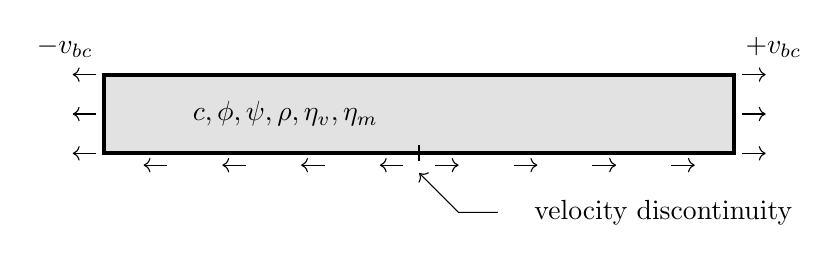
\begin{tikzpicture}
%\draw[fill=gray!23,gray!23](0,0) rectangle (10,3);
%\draw[step=0.5cm,gray,very thin] (0,0) grid (10,3); %background grid

\draw[fill=gray!23,gray!23](1,1) rectangle (9,2);

\draw[line width=0.5mm] (1,1)--(9,1)--(9,2)--(1,2)--cycle ;   

\draw[line width=0.3mm] (5,0.9)--(5,1.1); 

%left arrows
\draw [->] (0.9,1) -- (0.6,1);
\draw [->] (0.9,1.5) -- (0.6,1.5);
\draw [->] (0.9,2) -- (0.6,2);

\draw [->] (4.8,0.85) -- (4.5,0.85);
\draw [->] (3.8,0.85) -- (3.5,0.85);
\draw [->] (2.8,0.85) -- (2.5,0.85);
\draw [->] (1.8,0.85) -- (1.5,0.85);

%right arrows
\draw [->] (9.1,1) -- (9.4,1);
\draw [->] (9.1,1.5) -- (9.4,1.5);
\draw [->] (9.1,2) -- (9.4,2);

\draw [->] (5.2,0.85) -- (5.5,0.85);
\draw [->] (6.2,0.85) -- (6.5,0.85);
\draw [->] (7.2,0.85) -- (7.5,0.85);
\draw [->] (8.2,0.85) -- (8.5,0.85);

\node[] at (0.5,2.35) {$-v_{bc}$};
\node[] at (9.5,2.35) {$+v_{bc}$};

\node[] at (3.3,1.5) {$c,\phi,\psi,\rho,\eta_v,\eta_m$};
  
\draw [->] (6,0.25) -- (5.5,0.25) -- (5,0.75);
\node[] at (8.1,0.25) {velocity discontinuity};

\end{tikzpicture}
\end{center}


Extensional boundary conditions are as follows: 
\begin{itemize}
\item left boundary: $u=- \upnu_{bc}$, $v$ free;
\item right boundary: $u=+ \upnu_{bc}$, $v$ free; 
\item bottom boundary: $v=0$, $u=- \upnu_{bc}$ for $x<L_x/2$,  $u=+ \upnu_{bc}$ for $x>L_x/2$, and $u=0$ if $x=L_x/2$;
\item top boundary: zero traction.
\end{itemize}
For compressional boundary conditions the signs of all horizontal velocities should be reversed.
The nonlinear tolerance is set to $\text{tol}=10^{-6}$. Nonlinear iterations stop when 
maximum of the normalised nonlinear residual reaches the desired tolerance.
$\upnu_{bc}$ is chosen so that the background strain rate is $\dot\varepsilon_{bckgr}=10^{-15}\si{\per\second}$, 
i.e. $\upnu_{bc}=\dot\varepsilon_{bckgr} L_x/2$.

Following Choi \& Petersen \cite{chpe15}, we run the experiment with an associative ($\phi=\psi$) plasticity
and a non associative one ($\psi=0$, i.e. $R=0$). This second approach is essentially what many codes do (
i.e. $\vec\nabla\cdot\vec\upnu = 0$). We can also run the model with $\phi=\psi=0\si{\degree}$ so that 
we recover the von Mises plasticity yield criterion which is independent of pressure.  

The velocity, pressure, strain rate, dilation rate, and velocity divergence are shown hereunder both in 
extension and compression. Note that the domain has been substantially extended in the horizontal 
direction because of the wide shear band angles obtained in compression. It is now 80\si{\km} long 
and 10\si{\km} high (aspect ratio 8:1). 

Three angles are mechanically stable (e.g. \cite{kaus10}):
\[
\theta=\frac{\pi}{4}\pm \frac{\psi}{2} \qquad \text{Roscoe angle}
\]
\[
\theta=\frac{\pi}{4}\pm \frac{\phi}{2} \qquad \text{Coulomb angle}
\]
\[
\theta=\frac{\pi}{4}\pm \frac{\phi+\phi}{4} \qquad \text{Arthur angle}
\]
In the case of associative plasticity, $\phi=\psi$, so that all three angles are the same. 
Per row of elements, nodes or quadrature points, and per half of the domain (left and right) we find the location
with the highest strain-rate and record their coordinates.


\newpage
{\bf Extension}

\begin{center}
\includegraphics[width=.3\linewidth]{python_codes/fieldstone_39/benchmark1/extension/conv_phi0_psi0_etam0.pdf}
\includegraphics[width=.3\linewidth]{python_codes/fieldstone_39/benchmark1/extension/conv_phi0_psi0_etam19.pdf}
\includegraphics[width=.3\linewidth]{python_codes/fieldstone_39/benchmark1/extension/conv_phi0_psi0_etam20.pdf}\\
\includegraphics[width=.3\linewidth]{python_codes/fieldstone_39/benchmark1/extension/conv_phi30_psi0_etam0.pdf}
\includegraphics[width=.3\linewidth]{python_codes/fieldstone_39/benchmark1/extension/conv_phi30_psi0_etam19.pdf}
\includegraphics[width=.3\linewidth]{python_codes/fieldstone_39/benchmark1/extension/conv_phi30_psi0_etam20.pdf}\\
\includegraphics[width=.3\linewidth]{python_codes/fieldstone_39/benchmark1/extension/conv_phi30_psi30_etam0.pdf}
\includegraphics[width=.3\linewidth]{python_codes/fieldstone_39/benchmark1/extension/conv_phi30_psi30_etam19.pdf}
\includegraphics[width=.3\linewidth]{python_codes/fieldstone_39/benchmark1/extension/conv_phi30_psi30_etam20.pdf}\\
\includegraphics[width=.3\linewidth]{python_codes/fieldstone_39/benchmark1/extension/line_sr_phi0_psi0_etam0.pdf}
\includegraphics[width=.3\linewidth]{python_codes/fieldstone_39/benchmark1/extension/line_sr_phi0_psi0_etam19.pdf}
\includegraphics[width=.3\linewidth]{python_codes/fieldstone_39/benchmark1/extension/line_sr_phi0_psi0_etam20.pdf}\\
\includegraphics[width=.3\linewidth]{python_codes/fieldstone_39/benchmark1/extension/line_sr_phi30_psi0_etam0.pdf}
\includegraphics[width=.3\linewidth]{python_codes/fieldstone_39/benchmark1/extension/line_sr_phi30_psi0_etam19.pdf}
\includegraphics[width=.3\linewidth]{python_codes/fieldstone_39/benchmark1/extension/line_sr_phi30_psi0_etam20.pdf}\\
\includegraphics[width=.3\linewidth]{python_codes/fieldstone_39/benchmark1/extension/line_sr_phi30_psi30_etam0.pdf}
\includegraphics[width=.3\linewidth]{python_codes/fieldstone_39/benchmark1/extension/line_sr_phi30_psi30_etam19.pdf}
\includegraphics[width=.3\linewidth]{python_codes/fieldstone_39/benchmark1/extension/line_sr_phi30_psi30_etam20.pdf}\\
\end{center}
%\includegraphics[width=.3\linewidth]{python_codes/fieldstone_39/benchmark1/extension/line_eta_etam0.pdf}
%\includegraphics[width=.3\linewidth]{python_codes/fieldstone_39/benchmark1/extension/line_eta_etam19.pdf}
%\includegraphics[width=.3\linewidth]{python_codes/fieldstone_39/benchmark1/extension/line_eta_etam20.pdf}\\

\newpage
\begin{center}
\includegraphics[width=.3\linewidth]{python_codes/fieldstone_39/benchmark1/extension/shear_band_phi0_psi0_etam0.pdf}
\includegraphics[width=.3\linewidth]{python_codes/fieldstone_39/benchmark1/extension/shear_band_phi0_psi0_etam19.pdf}
\includegraphics[width=.3\linewidth]{python_codes/fieldstone_39/benchmark1/extension/shear_band_phi0_psi0_etam20.pdf}\\
\includegraphics[width=.3\linewidth]{python_codes/fieldstone_39/benchmark1/extension/shear_band_phi30_psi0_etam0.pdf}
\includegraphics[width=.3\linewidth]{python_codes/fieldstone_39/benchmark1/extension/shear_band_phi30_psi0_etam19.pdf}
\includegraphics[width=.3\linewidth]{python_codes/fieldstone_39/benchmark1/extension/shear_band_phi30_psi0_etam20.pdf}\\
\includegraphics[width=.3\linewidth]{python_codes/fieldstone_39/benchmark1/extension/shear_band_phi30_psi30_etam0.pdf}
\includegraphics[width=.3\linewidth]{python_codes/fieldstone_39/benchmark1/extension/shear_band_phi30_psi30_etam19.pdf}
\includegraphics[width=.3\linewidth]{python_codes/fieldstone_39/benchmark1/extension/shear_band_phi30_psi30_etam20.pdf}
\end{center}


\newpage
One can also run the extension model for $\phi=\psi={0,5,10,15,20,25,30}\degree$:
\begin{center}
\includegraphics[width=.45\linewidth]{python_codes/fieldstone_39/images/sr_0_30}
\includegraphics[width=.45\linewidth]{python_codes/fieldstone_39/images/etaeff_0_30}\\
\end{center}




\begin{center}
\includegraphics[width=.45\linewidth]{python_codes/fieldstone_39/images/shear_bands}
\includegraphics[width=.45\linewidth]{python_codes/fieldstone_39/images/shear_bands_nonass}\\
Results obtained on a 240x24 grid, max 50 nl iterations.
\end{center}


Note that benchmarking this in not easy. One solution Timo and I found was to add a 
velocity field $\underline{\vec\upnu}=(x,y,z)$ (with $\vec\nabla\cdot\underline{\vec\upnu}=3$)
to an existing analytical problem, e.g. the Burstedde benchamrk.

\newpage
%...........................................................
\subsection*{Benchmark \#2 - Spiegelman et al (2016) brick}

The setup is {\sl similar} to the one in Spiegelman et al (2016) \cite{spmw16}. 
It is a 2D Cartesian domain filled with an 
isoviscous layer at the bottom and a visco-plastic material on top, as shown here:  

\begin{center}
\includegraphics[width=6cm]{python_codes/fieldstone_39/images/spmw_1.png}
\includegraphics[width=8cm]{python_codes/fieldstone_39/images/spmw_2.png}
\end{center}

The domain has dimensions $L_x=128\si{\kilo\metre}$, $L_y=Lx/4$. 
The lower layer depth is $L_y/4$. The notch has dimensions $w=4\si{\kilo\metre}$
and $h=2\si{\kilo\metre}$. 

In what follows the nonlinear tolerance is set to $10^{-6}$. Due to a lack of resolution, I do not
implement the rounded edges of the seed. $U_0$ is set to $25\si{\mm\per\year}$ 
and the background viscosity of the brittle layer
is set to $\eta_v=10^{24}\si{\pascal\second}$. 

Note that the pressure colour bars in Fig(6) of \cite{spmw16} are most likely not correct at all: 
\begin{center}
\includegraphics[width=12cm]{python_codes/fieldstone_39/images/spmw_3.png}\\
{\captionfont Fig.(6) from Spiegelman et al (2016) \cite{spmw16}.}
\end{center}





\newpage
%........................................................
\subsection*{Benchmark \#4: Shortening of a visco-plastic bloc - part 1}

This benchmark originates in the book of Gerya. In the first edition the domain is 1000x1000km, 
while it is 100x100km in the second. We keep the second edition as a guideline. The benchmark
is actually elasto-visco-plastic but in this stone we neglect the elastic deformation. The 
boundary conditions are shown here:

\begin{center}
\includegraphics[width=6cm]{python_codes/fieldstone_39/results_shortening_block/setup}\\
{\captionfont Taken from \cite{gery19book}.}
\end{center}

The velocity on the boundaries is $\upnu_{bc}=5\cdot 10^{-9}$ \si{\metre\per\second} so that the background strain rate is 
$2 \upnu_{bc}/L = 10^{-13}\si{\per\second}$.
The weak medium and the weak inclusion have a viscosity $\eta=10^{17}\si{\pascal\second}$ while 
the block is visco-plastic, with $\eta=10^{23}\si{\pascal\second}$, $c=10^8\si{\pascal}$ 
and $\phi=37\degree$. 
Pressure is set to zero in the top right corner and later post-processed so as to insure a zero 
volume average.

In the case of von Mises ($\phi=0$) we expect the shear bands at $45\degree$. When $\phi>0$, as mentioned above
we expect:
\[
\frac{\pi}{4}-\frac{\phi}{2}=26.5\degree
\qquad
\frac{\pi}{4}-\frac{\phi}{4}=35.75\degree
\]

\begin{center}
\includegraphics[width=8cm]{python_codes/fieldstone_39/results_shortening_block/line}
\includegraphics[width=8cm]{python_codes/fieldstone_39/results_shortening_block/angles}\\
{\captionfont a) Line on which strain rate is measured. b) possible shear band angles:
green is $45\degree$, blue is $35.75\degree$ and red is $26.5\degree$.}
\end{center}


I have adapted slightly the dimensions inside the domain such that resolutions 16x16, 32x32, etc...
all showcase elements whose sides exactly align with the material interfaces. The size of the inclusion is 
$L/8=12.5$km and the block has a thickness of 50km:

\begin{center}
\includegraphics[width=10cm]{python_codes/fieldstone_39/results_shortening_block/geometry}\\
{\captionfont Material geometry for resolutions 16x16, 32x32 and 64x64.}
\end{center}


\newpage
\underline{von Mises (no dilation rate):}

\begin{center}
\includegraphics[width=5cm]{python_codes/fieldstone_39/results_shortening_block/u}
\includegraphics[width=5cm]{python_codes/fieldstone_39/results_shortening_block/v}
\includegraphics[width=5cm]{python_codes/fieldstone_39/results_shortening_block/vel}\\
{\captionfont Velocity field for 128x128, $\eta_m=1e19$}
\end{center}

\begin{center}
\includegraphics[width=8cm]{python_codes/fieldstone_39/results_shortening_block/etaeff}
\includegraphics[width=8cm]{python_codes/fieldstone_39/results_shortening_block/p}\\
\includegraphics[width=8cm]{python_codes/fieldstone_39/results_shortening_block/sr_elt_log}
\includegraphics[width=8cm]{python_codes/fieldstone_39/results_shortening_block/sr_elt}\\
{\captionfont From left to right: resolutions are 16x16, 32x32, 64x64 and 96x96. 100 nonlinear Picard iterations.}
\end{center}

\begin{center}
\includegraphics[width=5cm]{python_codes/fieldstone_39/results_shortening_block/conv_vM.pdf}
\includegraphics[width=5cm]{python_codes/fieldstone_39/results_shortening_block/sr_line_vM.pdf}
\includegraphics[width=5cm]{python_codes/fieldstone_39/results_shortening_block/sr_line_vM_reg.pdf}\\
{\captionfont $\eta_m=1e19$}
\end{center}




\newpage
\underline{viscous damper, no dilation rate, Drucker-Prager, phi=37:}


\begin{center}
\includegraphics[width=8cm]{python_codes/fieldstone_39/results_shortening_block/conv_DP.pdf}
\includegraphics[width=8cm]{python_codes/fieldstone_39/results_shortening_block/conv_DP_1e19.pdf}\\
{\captionfont Left: $\eta_m=0$, right: $\eta_m=10^{19}$}
\end{center}


\begin{center}
\includegraphics[width=4cm]{python_codes/fieldstone_39/results_shortening_block/32x32_phi37_1e19/sr}
\includegraphics[width=4cm]{python_codes/fieldstone_39/results_shortening_block/32x32_phi37_1e19/sr_log}
\includegraphics[width=4cm]{python_codes/fieldstone_39/results_shortening_block/32x32_phi37_1e19/p}
\includegraphics[width=4cm]{python_codes/fieldstone_39/results_shortening_block/32x32_phi37_1e19/eta}\\
{\captionfont Fieldstone 32x32}\\
\includegraphics[width=4cm]{python_codes/fieldstone_39/results_shortening_block/aspect_32x32_1e19_phi37/sr}
\includegraphics[width=4cm]{python_codes/fieldstone_39/results_shortening_block/aspect_32x32_1e19_phi37/sr_log}
\includegraphics[width=4cm]{python_codes/fieldstone_39/results_shortening_block/aspect_32x32_1e19_phi37/p}
\includegraphics[width=4cm]{python_codes/fieldstone_39/results_shortening_block/aspect_32x32_1e19_phi37/eta}\\
\includegraphics[width=4cm]{python_codes/fieldstone_39/results_shortening_block/aspect_64x64_1e19_phi37/sr}
\includegraphics[width=4cm]{python_codes/fieldstone_39/results_shortening_block/aspect_64x64_1e19_phi37/sr_log}
\includegraphics[width=4cm]{python_codes/fieldstone_39/results_shortening_block/aspect_64x64_1e19_phi37/p}
\includegraphics[width=4cm]{python_codes/fieldstone_39/results_shortening_block/aspect_64x64_1e19_phi37/eta}\\
{\captionfont ASPECT 32x32, 64x64} 
\end{center}



\newpage
To explore:

- associative and non-associative drucker-prage

- visco-plastic vs visco-viscoplastic







\newpage
%..............................................
\subsection*{Benchmark \#5: Shortening of a visco-plastic bloc - part 2}

The setup originates in Duretz et al (2018) \cite{dusd18} and is also carried out 
in Jacquey \& Cacace (2020) \cite{jaca20a}. We here again neglect the elastic 
deformation. 
The domain is 4x2 km. There is a linear viscous inclusion in the middle of radius 100\si{\metre} and 
viscosity $\eta_{inc}=10^{17}\si{\pascal\second}$. The material around is characterised by 
$\eta_v=10^{24}\si{pascal\second}$, $c=3e7\si{pascal}$, $\phi=30\degree$, $psi=10\degree$.
Boundary conditions are as follows: 

\begin{center}
\includegraphics[width=6cm]{python_codes/fieldstone_39/results_shortening_block2/jaca20a}
\end{center}

In the papers they prescribe $\Delta \varepsilon = 5\cdot 10^{-5}$ over a 
time step of $\Delta t=10^{10}\si{second}$, 
i.e. the background strain rate is $\dot\varepsilon=5\cdot 10^{-15}\si{\per\second}$.
Given $L_x$ and $L_y$ we can easily arrive at the velocity values to be prescribed:
\[
|u_{bc}|=\dot{\varepsilon}_{bc} L_x/2
\qquad
|v_{bc}|=\dot{\varepsilon}_{bc} L_y/2
\]
 
The inclusion is circular, i.e. no amount of mesh refinement will be such that the mesh 
edges align with it, as opposed to the previous experiment. 


\begin{center}
\includegraphics[width=8cm]{python_codes/fieldstone_39/results_shortening_block2/dusd18}
\includegraphics[width=8cm]{python_codes/fieldstone_39/results_shortening_block2/jaca20b}\\
{\captionfont Left: taken from Duretz et al (2018) \cite{dusd18}; Right: taken from Jacquey \& Cacace (2020) \cite{jaca20a}.
Note that these simulations have been run with elasto-visco-plastic rheologies 
for a certain amount of time so that the propagation of the shear bands is not final/complete, as
opposed to the converged visco-plastic solutions shown hereafter.}
\end{center}

As before, pressure is set to zero in the top right corner, and further post processed to insure that its volume 
average is zero.


\clearpage
\subsubsection*{von Mises rheology}

\begin{center}
\includegraphics[width=8cm]{python_codes/fieldstone_39/results_shortening_block2/conv_vM}\\
{\captionfont Nonlinear convergence, fieldstone and aspect, 128x64, 200 nonlinear iterations, $\eta_m=10^{19}$.}
\end{center}
\begin{center}
\includegraphics[width=5.8cm]{python_codes/fieldstone_39/results_shortening_block2/128x64_1e19/u}
\includegraphics[width=5.8cm]{python_codes/fieldstone_39/results_shortening_block2/128x64_1e19/v}
\includegraphics[width=5.8cm]{python_codes/fieldstone_39/results_shortening_block2/128x64_1e19/vel}\\
\includegraphics[width=5.8cm]{python_codes/fieldstone_39/results_shortening_block2/128x64_1e19/eta}
\includegraphics[width=5.8cm]{python_codes/fieldstone_39/results_shortening_block2/128x64_1e19/sr}
\includegraphics[width=5.8cm]{python_codes/fieldstone_39/results_shortening_block2/128x64_1e19/p}\\
{\captionfont 128x64, 200 nonlinear iterations, $\eta_m=10^{19}$}
\end{center}

\begin{center}
\includegraphics[width=5.8cm]{python_codes/fieldstone_39/results_shortening_block2/aspect_128x64_1e19/u}
\includegraphics[width=5.8cm]{python_codes/fieldstone_39/results_shortening_block2/aspect_128x64_1e19/v}
\includegraphics[width=5.8cm]{python_codes/fieldstone_39/results_shortening_block2/aspect_128x64_1e19/vel}\\
\includegraphics[width=5.8cm]{python_codes/fieldstone_39/results_shortening_block2/aspect_128x64_1e19/eta}
\includegraphics[width=5.8cm]{python_codes/fieldstone_39/results_shortening_block2/aspect_128x64_1e19/sr}
\includegraphics[width=5.8cm]{python_codes/fieldstone_39/results_shortening_block2/aspect_128x64_1e19/p}\\
{\captionfont ASPECT: 128x64, 200 nonlinear iterations, $\eta_m=10^{19}$}
\end{center}

\newpage
In order to help the comparison, I plot the effective viscosity and the strain rate for both next to one another:
\begin{center}
\includegraphics[width=8cm]{python_codes/fieldstone_39/results_shortening_block2/eta_both}
\includegraphics[width=8cm]{python_codes/fieldstone_39/results_shortening_block2/sr_both}\\
{\captionfont Left half is fieldstone, Right half is aspect.}
\end{center}


\begin{center}
\includegraphics[width=10cm]{python_codes/fieldstone_39/results_shortening_block2/sr_line_vM.pdf}\\
{\captionfont Strain rate cross section at $y=11L_y/16$.}
\end{center}


\clearpage
\subsubsection*{Drucker-Prager rheology ($\phi=30\degree$)}

\includegraphics[width=8cm]{python_codes/fieldstone_39/results_shortening_block2/conv_DP}
\includegraphics[width=8cm]{python_codes/fieldstone_39/results_shortening_block2/sr_line_DP.pdf}

\begin{center}
\includegraphics[width=4cm]{python_codes/fieldstone_39/results_shortening_block2/32x16_1e19_phi30/vel}
\includegraphics[width=4cm]{python_codes/fieldstone_39/results_shortening_block2/32x16_1e19_phi30/p}
\includegraphics[width=4cm]{python_codes/fieldstone_39/results_shortening_block2/32x16_1e19_phi30/sr}
\includegraphics[width=4cm]{python_codes/fieldstone_39/results_shortening_block2/32x16_1e19_phi30/eta}\\
\includegraphics[width=4cm]{python_codes/fieldstone_39/results_shortening_block2/48x24_1e19_phi30/vel}
\includegraphics[width=4cm]{python_codes/fieldstone_39/results_shortening_block2/48x24_1e19_phi30/p}
\includegraphics[width=4cm]{python_codes/fieldstone_39/results_shortening_block2/48x24_1e19_phi30/sr}
\includegraphics[width=4cm]{python_codes/fieldstone_39/results_shortening_block2/48x24_1e19_phi30/eta}\\
\includegraphics[width=4cm]{python_codes/fieldstone_39/results_shortening_block2/64x32_1e19_phi30/vel}
\includegraphics[width=4cm]{python_codes/fieldstone_39/results_shortening_block2/64x32_1e19_phi30/p}
\includegraphics[width=4cm]{python_codes/fieldstone_39/results_shortening_block2/64x32_1e19_phi30/sr}
\includegraphics[width=4cm]{python_codes/fieldstone_39/results_shortening_block2/64x32_1e19_phi30/eta}\\
\includegraphics[width=4cm]{python_codes/fieldstone_39/results_shortening_block2/128x64_1e19_phi30/vel}
\includegraphics[width=4cm]{python_codes/fieldstone_39/results_shortening_block2/128x64_1e19_phi30/p}
\includegraphics[width=4cm]{python_codes/fieldstone_39/results_shortening_block2/128x64_1e19_phi30/sr}
\includegraphics[width=4cm]{python_codes/fieldstone_39/results_shortening_block2/128x64_1e19_phi30/eta}\\
{\captionfont Fielstone. Top to bottom: 32x16, 48x24, 64x32, 128x64, etam=1e19, phi=30}\\
\includegraphics[width=4cm]{python_codes/fieldstone_39/results_shortening_block2/aspect_32x16_1e19_phi30/vel}
\includegraphics[width=4cm]{python_codes/fieldstone_39/results_shortening_block2/aspect_32x16_1e19_phi30/p}
\includegraphics[width=4cm]{python_codes/fieldstone_39/results_shortening_block2/aspect_32x16_1e19_phi30/sr}
\includegraphics[width=4cm]{python_codes/fieldstone_39/results_shortening_block2/aspect_32x16_1e19_phi30/eta}\\
\includegraphics[width=4cm]{python_codes/fieldstone_39/results_shortening_block2/aspect_64x32_1e19_phi30/vel}
\includegraphics[width=4cm]{python_codes/fieldstone_39/results_shortening_block2/aspect_64x32_1e19_phi30/p}
\includegraphics[width=4cm]{python_codes/fieldstone_39/results_shortening_block2/aspect_64x32_1e19_phi30/sr}
\includegraphics[width=4cm]{python_codes/fieldstone_39/results_shortening_block2/aspect_64x32_1e19_phi30/eta}\\
{\captionfont ASPECT, 64x32, etam=1e19, phi=30}\\
\end{center}

Note that ASPECT does not use the proper partitioning of strain rates, and uses total strain rate 
in plastic element. This could explain the difference?



\clearpage
\subsubsection*{A very different approach: diffusion plasticity}

The idea is to solve a diffusion equation for each component of the strain rate tensor. In 
order to do so, we need nodal values of this tensor and these values must then also be used in 
the rheology: the shape functions are used to interpolate these values onto the quadrature points
(as opposed to the standard way of using the shape function derivatives to interpolate the velocity). 

After each nonlinear iteration the nodal fields $\dot{\varepsilon}_{xx}$, $\dot{\varepsilon}_{yy}$ 
and $\dot{\varepsilon}_{xy}$ are diffused. The diffusion coefficient $D$ value is not straightforward
to choose. Also, boundary conditions are unknown so we resort to doing nothing, i.e. zero Neumann 
boundary conditions.

Note that in this case we have $\eta_m=0$ and that it is tTriggered in the code 
by {\sl use\_srn\_diff=True}.

\begin{center}
\includegraphics[width=8cm]{python_codes/fieldstone_39/results_shortening_block2/diffusion/srn}
\includegraphics[width=8cm]{python_codes/fieldstone_39/results_shortening_block2/diffusion/eta}\\
{\captionfont resolution 32x16, from top to bottom $D=0,2h_x,8h_x$.}
\end{center}

\begin{center}
\includegraphics[width=8cm]{python_codes/fieldstone_39/results_shortening_block2/diffusion/conv.pdf}
\end{center}

The diffusion helps with convergence. Rather importantly, it requires the use of nodal strainrate 
in the rheology, as opposed to before where strain rate at the quadrature point was computed using 
the derivatives of the shape functions. 


\begin{center}
\includegraphics[width=5cm]{python_codes/fieldstone_39/results_shortening_block2/diffusion/sr_lots}
\includegraphics[width=5cm]{python_codes/fieldstone_39/results_shortening_block2/diffusion/eta_lots}
\includegraphics[width=5cm]{python_codes/fieldstone_39/results_shortening_block2/diffusion/p_lots}\\
{\captionfont D=1km, 32x16, 48x24, 64x32, 80x40, 96x48}
\end{center}

\begin{center}
\includegraphics[width=10cm]{python_codes/fieldstone_39/results_shortening_block/diffusion/sr_line.pdf}\\
{\captionfont Strain rate cross section at $y=11L_y/16$.}
\end{center}


 %%%%%%%%%%%%%%%%%%%%%%%%%%%%%%%%%%%%%%%%%%%%%%%%%%%%%%%%%%%

\chapter{Instantaneous Rayleigh-Taylor instability (\QtwoQone) \label{f40}} %%%%%%%%%%%%%%%%%%%%%%% 40
\lstinputlisting[language=bash,basicstyle=\small]{python_codes/fieldstone_40/keywords.ascii}

\begin{center}
Code at \url{https://github.com/cedrict/fieldstone/tree/master/python_codes/fieldstone_40}
\end{center}

\par\noindent\rule{\textwidth}{0.4pt}
%%%%%%%%%%%%%%%%%%%%%%%%%%%%%%%%%%%%%%%%%%%%%%%%%%%%%%%%%%%%%%%%%%%%%%%%%%%%%%%%%%%%%%%%%%%%

This benchmark is carried out in \textcite{deka08} (2008), \textcite{gery10} (2010) and \textcite{thie11} (2011) 
and is based on the analytical solution by \textcite{ramb68} (1968). 
It consists of a buoyancy-driven two-layer system driven. 
The domain is a square of size $512\times512$km. 
Free slip are imposed on the sides while no-slip boundary conditions are imposed on the
top and the bottom of the box.

Fluid 1 $(\rho_1,\eta_1)$ of thickness $h_1$ overlays 
fluid 2 $(\rho_2,\eta_2)$ of thickness $h_2$ (with $h_1+h_2=L_y$).
An initial sinusoidal disturbance of the interface between these
layers is introduced and is characterised by an amplitude $\Delta$ and a
wavelength $\lambda=L_x/2$ as shown here: 

\begin{center}
a) \includegraphics[width=0.38\textwidth]{python_codes/fieldstone_40/images/setup}
b) \includegraphics[width=0.55\textwidth]{python_codes/fieldstone_40/images/dens}\\
{\captionfont  a) Setup of the experiment, taken from \cite{thie11}; b) grid setup for 24$\times$24 grid.} 
\end{center}

Under this condition, the velocity of the diapiric growth
$v_y$ is given by the relation
\[
\frac{v_y}{\Delta} = - K \frac{\rho_1-\rho_2}{2 \eta_2} h_2 g
\]
with the dimensionless growth factor $K$ being
\[
K=\frac{-d_{12}}{c_{11}j_{22}-d_{12}i_{21}}
\]
and 
\begin{eqnarray}
c_{11} &=& \frac{\eta_1 2 \phi_1^2}{\eta_2(\cosh 2\phi_1 - 1 - 2\phi_1^2)} - \frac{2\phi_2^2}{\cosh 2\phi_2 - 1 - 2 \phi_2^2}\\
d_{12} &=& \frac{\eta_1(\sinh 2\phi_1 -2\phi_1)}{\eta_2(\cosh 2\phi_1 -1 -2\phi_1^2)} + \frac{\sinh 2\phi_2 - 2\phi_2}{\cosh 2\phi_2 -1 -2\phi_2^2} \\
i_{21} &=& \frac{\eta_1\phi_2 (\sinh 2 \phi_1 + 2 \phi_1)}{\eta_2(\cosh 2\phi_1 -1 -2\phi_1^2)} 
+ \frac{\phi_2 (\sinh 2\phi_2 + 2\phi_2)}{\cosh 2\phi_2 -1 -2\phi_2^2} \\
j_{22} &=& \frac{\eta_1 2 \phi_1^2 \phi_2}{\eta_2(\cosh 2\phi_1 -1-2\phi_1^2)} - \frac{2\phi_2^3}{ \cosh 2\phi_2 -1 -2\phi_2^2}\\
\phi_1&=&\frac{2\pi h_1}{\lambda}\\
\phi_2&=&\frac{2\pi h_2}{\lambda}
\end{eqnarray}


\begin{center}
\includegraphics[width=7cm]{python_codes/fieldstone_40/images/vel}
\includegraphics[width=7cm]{python_codes/fieldstone_40/images/p}
\end{center}


\begin{center}
\includegraphics[width=5cm]{python_codes/fieldstone_40/images/plot24x24}
\includegraphics[width=5cm]{python_codes/fieldstone_40/images/plot32x32}
\includegraphics[width=5cm]{python_codes/fieldstone_40/images/plot48x48}\\
{\captionfont  Left: 24$\times$24 elements, middle: 32$\times$32; right: 48$\times$48. We see that 
increasing resolution yields more accurate results in the cases of short wavelength 
perturbations (points on the right on the plots).\\  
Note that in \cite{thie11} I fixed $\lambda=L_x/2$ and varied $L_x$. Here I keep $L_x$ fixed
and vary $\lambda=L_x/2,L_x,4,L_x/8$. Each line corresponds to a different value of the viscosity $\eta_2$.} 
\end{center}


 %%%%%%%%%%%%%%%%%%%%%%%%%%%%%%%%%%%%%%%%%%%%%%%%%%%%%%%%%%%

\chapter{Stokes flow and structural restoration (\QtwoQone) \label{f41}} %%%%%%%%%%%%%%%%%%%%%%%%%% 41

\paragraph{Setup of the experiment} It originates in Schuh-Senlis \etal \cite{sctc20} 
and is a scaled-up version of the Rayleigh-Taylor experiment of van Keken et al (1997) \cite{vaks97}.
In the original experiment the domain is $0.9142\times1$, viscosity is $\eta=100$, 
densities are 1000 and 1010 (i.e. $\delta \rho=10$) and the gravity is $|\vec{g}|=10$.
In our case the domain is 10,000 times larger, i.e. $9142\times10000$m, 
our viscosity is $\eta=10^{19}$, our densities are 2150 and 2600, i.e. $\delta\rho = 450$, 
and we also set $|\vec{g}|=10$.

\begin{center}
\includegraphics[width=7cm]{python_codes/fieldstone_41/images/setup}
\end{center}

Boundary conditions are no slip on the top and bottom, free slip on the sides.

In the original paper, 
length=1, viscosity=100, gravity =10, density contrast =10 and time unit =1,
so the dimensionless quantity
\[
\frac{\eta}{\delta\rho \cdot g \; length \cdot time} = \frac{100}{10 \cdot 10 \cdot 1 \cdot 1} =1
\]
If we now run a geometrically similar experiment with 
length=10km, viscosity=$10^{19}$, gravity=10, density contrast=450 and time unit = $t$
then we should also have 
\[
\frac{\eta}{\delta\rho \cdot g \; length \cdot time} = \frac{10^{19}}{450 \cdot 10 \cdot 10^4 \cdot t} =1
\]
i.e.,
\[
t = \frac{10^{14}}{450} \simeq 2.222 \cdot 10^{11}\text{s}
\]
This means that in order to plot our results against those in van Keken et al, their results
must be scaled: times must be multiplied by $t$ and velocities divided by 
$t/length = 2.222 \cdot 10^{7}\text{m/s}$  

The initial mass of the system is:
\[
M(t=0) = L_x \times 2km \times \rho_s + Lx \times 8km \times \rho_0 = 
9142 \cdot(2000\cdot 2150 + 8000\cdot 2600) \simeq 2.294642\cdot 10^{11}\text{kg}
\]

\paragraph{The code} It is based on stable $Q_2\times Q_1$ elements for the Stokes equations and 
the heat transport equation need not be solved. 
It relies on the Particle-in-Cell method (see Section~\ref{MMM-ss:pic}) for material advection. 
At startup {\tt nmarker\_per\_dim**2} particles are regularly placed in each element. 
There are in total:
\begin{lstlisting}
nmarker=nmarker_per_element*nel
\end{lstlisting}

Markers track material number, i.e. 1 or 2:
\begin{lstlisting}
for im in range (0,nmarker):
    if swarm_y[im]>salt_thickness+amplitude*np.cos(np.pi*swarm_x[im]/Lx):
       swarm_mat[im]=2
    else:
       swarm_mat[im]=1
\end{lstlisting}

Marker density is interpolated onto the Q1 mesh by means of the Q1 shape functions:
\begin{lstlisting}
for im in range(0,nmarker):
    ielx=int(swarm_x[im]/Lx*nelx)
    iely=int(swarm_y[im]/Ly*nely)
    iel=nelx*(iely)+ielx
    N1=0.25*(1-swarm_r[im])*(1-swarm_s[im])
    N2=0.25*(1+swarm_r[im])*(1-swarm_s[im])
    N3=0.25*(1+swarm_r[im])*(1+swarm_s[im])
    N4=0.25*(1-swarm_r[im])*(1+swarm_s[im])
    rho_nodal[iconP[0,iel]]+=rho_mat[swarm_mat[im]-1]*N1
    rho_nodal[iconP[1,iel]]+=rho_mat[swarm_mat[im]-1]*N2
    rho_nodal[iconP[2,iel]]+=rho_mat[swarm_mat[im]-1]*N3
    rho_nodal[iconP[3,iel]]+=rho_mat[swarm_mat[im]-1]*N4
    rho_nodal_counter[iconP[0,iel]]+=N1
    rho_nodal_counter[iconP[1,iel]]+=N2
    rho_nodal_counter[iconP[2,iel]]+=N3
    rho_nodal_counter[iconP[3,iel]]+=N4
rho_nodal/=rho_nodal_counter
\end{lstlisting}
This is a marker-centric approach, which is identical to the 
somewhat more instinctive node-centric approach which itself is similar
to the meshless methods approach (think of the SPH method kernel but with a 
square support). Density is later on interpolated onto the quadrature points 
with the $Q_1$ shape functions again to avoid the problems highlighted in 
Section~\ref{MMM-ss:bern}.
Viscosity is averaged per element by means of an arithmetic, geometric or harmonic mean.

Particles are advected by means of a (space) Runge-Kutta 1st/2nd/3rd order algorithm (see
Section~\ref{MMM-ss:rkm}). The time step $\delta t$ is set by means of the CFL criterion (see
Section~\ref{MMM-ss:cfl}).

The root mean square velocity and total mass of the system are computed every time step.

Simulations end when the maximum number of time steps is reached or when 
an element does not contain any particle.
\begin{center}
\includegraphics[width=7cm]{python_codes/fieldstone_41/results/vrms_RK.pdf}
\includegraphics[width=7cm]{python_codes/fieldstone_41/results/vrms_RES.pdf}\\
\includegraphics[width=7cm]{python_codes/fieldstone_41/results/vrms_CFL.pdf}
\includegraphics[width=7cm]{python_codes/fieldstone_41/results/vrms_nmarker.pdf}\\
{\captionfont Root mean square velocity as a function of time. Black curves are those in van Keken
et al (1997). Letters stand for authors initials.}
\end{center}



\begin{center}
\includegraphics[width=7cm]{python_codes/fieldstone_41/results/mass.pdf}
\includegraphics[width=7cm]{python_codes/fieldstone_41/results/nmarker.pdf}
\end{center}

\begin{center}
\includegraphics[width=5cm]{python_codes/fieldstone_41/results/64x64_10_RK3/markers0000}
\includegraphics[width=5cm]{python_codes/fieldstone_41/results/64x64_10_RK3/markers0143}
\includegraphics[width=5cm]{python_codes/fieldstone_41/results/64x64_10_RK3/rho_nodal_0143}\\
{\captionfont 64x64 simulation right before crash}
\end{center}


\newpage
%---------------------------------------------------------------
\subsection*{Stokes sphere under deformable free surface}

The setup is described in Section~\ref{MMM-ss:stokes_sphere_fs2D}. 
Densities are projected on the nodes or elements with an arithmetic averaging while
viscosities are projected onto elements ({\tt avrg}$>0$) or onto $Q_1$nodes ({\tt avrg}$<0$).
There are 7 averaging schemes implemented:
\begin{itemize}
\item[{\tt avrg}=-1] first-order basis function weighed arithmetic average onto nodes
\item[{\tt avrg}=-2] first-order basis function weighed geometric average onto nodes
\item[{\tt avrg}=-3] first-order basis function weighed harmonic average onto nodes
\item[{\tt avrg}=+1]  elemental piecewise constant arithmetic average 
\item[{\tt avrg}=+2]  elemental piecewise constant geometric average 
\item[{\tt avrg}=+3]  elemental piecewise constant harmonic average 
\item[{\tt avrg}=+4]  elemental first-order least square projection 
\end{itemize}

Let us recall that the Least Squares methodology is presented for example in 
Thielmann \etal \cite{thmk14} and in Section~\ref{MMM-ss:pic}:
the density or viscosity values carried by the markers are represented by a linear 
function in a 2D space inside each 
element, i.e. $\tilde{\eta}({\vec r}) = a + b x+c y$ and $\tilde{\rho}=d+ex+fy$.

When {\tt avrg}$<0$ values are projected onto quadrature points by means 
of $Q_1$ basis functions using the values at the corners of the element.
When {\tt avrg}$=1,2,3$ all quadrature points receive the same elemental value. 
When {\tt avrg}$=4$ the coordinates of each quadrature points are used in order to 
estimate the value from the coefficients $\{a,b,c\}$ and $\{d,e,f\}$ 
of the (limited) least square.

Given the current limitations of this simple code I can only run experiments with limited resolutions. 
Also since I later wish to plot the density and viscosity values carried by the quadrature points 
on a vertical line passing through the middle of the sphere, I focus on odd numbers of elements
in the horizontal direction and investigate $33\times33$, $49\times49$, $65\times65$, $81\times81$,
and $97\times97$.

\begin{center}
\includegraphics[width=5.5cm]{python_codes/fieldstone_41/results/exp3/markers}
\includegraphics[width=5.5cm]{python_codes/fieldstone_41/results/exp3/vel_line}\\
{\captionfont 
Left: markers on 33x33 grid, $5^2$ markers per element.  
Right: vertical component $v$ of the velocity as obtained \\
on the $81\times81$ mesh using least squares + limiter projection.\\
The black line indicates the location of profile measurements.}
\end{center}

\begin{center}
\includegraphics[width=4.25cm]{python_codes/fieldstone_41/results/exp3/33x33/profile_v.pdf}
\includegraphics[width=4.25cm]{python_codes/fieldstone_41/results/exp3/33x33/profile_p.pdf}
\includegraphics[width=4.25cm]{python_codes/fieldstone_41/results/exp3/33x33/profile_eta_elemental.pdf}
\includegraphics[width=4.25cm]{python_codes/fieldstone_41/results/exp3/33x33/profile_eta_nodal.pdf}\\
\includegraphics[width=4.25cm]{python_codes/fieldstone_41/results/exp3/49x49/profile_v.pdf}
\includegraphics[width=4.25cm]{python_codes/fieldstone_41/results/exp3/49x49/profile_p.pdf}
\includegraphics[width=4.25cm]{python_codes/fieldstone_41/results/exp3/49x49/profile_eta_elemental.pdf}
\includegraphics[width=4.25cm]{python_codes/fieldstone_41/results/exp3/49x49/profile_eta_nodal.pdf}\\
\includegraphics[width=4.25cm]{python_codes/fieldstone_41/results/exp3/65x65/profile_v.pdf}
\includegraphics[width=4.25cm]{python_codes/fieldstone_41/results/exp3/65x65/profile_p.pdf}
\includegraphics[width=4.25cm]{python_codes/fieldstone_41/results/exp3/65x65/profile_eta_elemental.pdf}
\includegraphics[width=4.25cm]{python_codes/fieldstone_41/results/exp3/65x65/profile_eta_nodal.pdf}\\
\includegraphics[width=4.25cm]{python_codes/fieldstone_41/results/exp3/81x81/profile_v.pdf}
\includegraphics[width=4.25cm]{python_codes/fieldstone_41/results/exp3/81x81/profile_p.pdf}
\includegraphics[width=4.25cm]{python_codes/fieldstone_41/results/exp3/81x81/profile_eta_elemental.pdf}
\includegraphics[width=4.25cm]{python_codes/fieldstone_41/results/exp3/81x81/profile_eta_nodal.pdf}\\
\includegraphics[width=4.25cm]{python_codes/fieldstone_41/results/exp3/97x97/profile_v.pdf}
\includegraphics[width=4.25cm]{python_codes/fieldstone_41/results/exp3/97x97/profile_p.pdf}
\includegraphics[width=4.25cm]{python_codes/fieldstone_41/results/exp3/97x97/profile_eta_elemental.pdf}
\includegraphics[width=4.25cm]{python_codes/fieldstone_41/results/exp3/97x97/profile_eta_nodal.pdf}\\
\includegraphics[width=4.25cm]{python_codes/fieldstone_41/results/exp3/113x113/profile_v.pdf}
\includegraphics[width=4.25cm]{python_codes/fieldstone_41/results/exp3/113x113/profile_p.pdf}
\includegraphics[width=4.25cm]{python_codes/fieldstone_41/results/exp3/113x113/profile_eta_elemental.pdf}
\includegraphics[width=4.25cm]{python_codes/fieldstone_41/results/exp3/113x113/profile_eta_nodal.pdf}\\
\includegraphics[width=4.25cm]{python_codes/fieldstone_41/results/exp3/129x129/profile_v.pdf}
\includegraphics[width=4.25cm]{python_codes/fieldstone_41/results/exp3/129x129/profile_p.pdf}
\includegraphics[width=4.25cm]{python_codes/fieldstone_41/results/exp3/129x129/profile_eta_elemental.pdf}
\includegraphics[width=4.25cm]{python_codes/fieldstone_41/results/exp3/129x129/profile_eta_nodal.pdf}\\
{\captionfont 
1st column: vertical velocity profile; 
2nd column: vertical pressure profile; 
3rd column: viscosity on quadrature points in log scale for {\tt avrg}$>0$ (elemental approach);
4th column: viscosity on quadrature points in log scale for {\tt avrg}$<0$ (nodal approach);
$5^2$ markers per element.
The black dot indicates the velocity in the middle of the sphere 
obtained with \stone 93 using Crouzeix-Raviart triangular elements.} 
\end{center}
It is immediately apparent that the least-square case yields smooth velocity profiles, even at 
low resolutions. Also it is clear that nodal approaches tend to smear out the transition zone
but do not yield a visible improvement in terms of velocity.

\begin{center}
\includegraphics[width=7.5cm]{python_codes/fieldstone_41/results/exp3/mass.pdf}
\includegraphics[width=7.5cm]{python_codes/fieldstone_41/results/exp3/vrms.pdf}\\
{\captionfont Total mass and root mean square velocity $\upnu_{rms}$ for all 7 projections.}
\end{center}

%-----------------------------------------------------------------------------
\subsubsection*{A word about the need for a limiter}

The following figures are obtained with a standard linear least square algorithm. 

\begin{center}
\includegraphics[width=7cm]{python_codes/fieldstone_41/results/exp3/rho_ls}
\includegraphics[width=7cm]{python_codes/fieldstone_41/results/exp3/eta_ls}\\
\includegraphics[width=7cm]{python_codes/fieldstone_41/results/exp3/rho_ls_warp}
\includegraphics[width=7cm]{python_codes/fieldstone_41/results/exp3/eta_ls_warp}\\
\includegraphics[width=7cm]{python_codes/fieldstone_41/results/exp3/rho_ls_warp2}
\includegraphics[width=7cm]{python_codes/fieldstone_41/results/exp3/eta_ls_warp2}\\
\end{center}

Describe here limiter...


 %%%%%%%%%%%%%%%%%%%%%%%%%%%%%%%%%%%%%%%%%%%%%%%%%%%%%%%%%%%

\chapter{The no flow test (\QonePzero, \QtwoQone, \QthreeQtwo, \QfourQthree)\label{f42}} %%%%%%%%%% 42
\lstinputlisting[language=bash,basicstyle=\small]{python_codes/fieldstone_42/keywords.ascii}

\begin{center}
Code at \url{https://github.com/cedrict/fieldstone/tree/master/python_codes/fieldstone_42}
\end{center}

\par\noindent\rule{\textwidth}{0.4pt}

%%%%%%%%%%%%%%%%%%%%%%%%%%%%%%%%%%%%%%%%%%%%%%%%%%%%%%%%%%%%%%%%%%%%%%%%%%%%%%%%%%%%%%%%%%%%


The idea behind this stone comes from the following excerpt of Fortin \& Fortin (1985) \cite{fofo85}:
\begin{center}
\includegraphics[width=14cm]{python_codes/fieldstone_42/images/fofo85a}\\
\includegraphics[width=14cm]{python_codes/fieldstone_42/images/fofo85b}
\end{center}

I then set out to reproduce this and to compare the results with continuous-pressure elements.
On the boundary of the domain $\Omega$ I impose $\vec\upnu=\vec{0}$ and 
the viscosity and density are set to 1. The gravity vector points downwards
with $|\vec{g}|=1$.
The analytical solution is $\vec\upnu(x,y)=\vec{0}$ and $p(x,y)=ay+b$, 
where the constants $a$ and $b$ are determined by the geometry and the buoyancy force.

Based on the figure above I set $L_x=16$ and $L_y=6$ and the angle is set to $45\degree$ (while it 
is about $15\degree$ on the figures below).
The chosen number of elements is $16\times 8$ as in \cite{fofo85}.
Rather arbitrarily the pressure is set to zero on the top right corner (This is not really
important since the pressure is defined up to a constant in this case).

I consider the following three different domain geometries:
\begin{center}
\input{python_codes/fieldstone_42/tikz_geoms}
\end{center}
and three different elements: ${\bm Q}_1\times P_0$, ${\bm Q}_2\times Q_1$, and ${\bm Q}_3\times Q_2$.

%.............................
\subsubsection*{geom=0}

I find that the checkerboard mode is present for the unstable ${\bm Q}_1\times P_0$
element. However, for all three elements the velocity is zero, down to machine precision.
For the two continuous-pressure elements the pressure at the top is 0 and 6 at the 
bottom as expected.

\begin{center}
\includegraphics[width=5.4cm]{python_codes/fieldstone_42/results/geom0/press1}
\includegraphics[width=5.4cm]{python_codes/fieldstone_42/results/geom0/press2}
\includegraphics[width=5.4cm]{python_codes/fieldstone_42/results/geom0/press3}\\
\includegraphics[width=5.4cm]{python_codes/fieldstone_42/results/geom0/vel1}
\includegraphics[width=5.4cm]{python_codes/fieldstone_42/results/geom0/vel2}
\includegraphics[width=5.4cm]{python_codes/fieldstone_42/results/geom0/vel3}\\
{\captionfont From left to right: ${\bm Q}_1\times P_0$, ${\bm Q}_2\times Q_1$, 
and ${\bm Q}_3\times Q_2$.}
\end{center}


%.............................
\subsubsection*{geom=1}

We find that the checkerboard mode is now absent and velocities are still zero
for all three elements. The pressure is hydrostatic and only depends on the $y$-coordinate.

\begin{center}
\includegraphics[width=5.1cm]{python_codes/fieldstone_42/results/geom1/press1}
\includegraphics[width=5.1cm]{python_codes/fieldstone_42/results/geom1/press2}
\includegraphics[width=5.1cm]{python_codes/fieldstone_42/results/geom1/press3}\\
\includegraphics[width=5.1cm]{python_codes/fieldstone_42/results/geom1/vel1}
\includegraphics[width=5.1cm]{python_codes/fieldstone_42/results/geom1/vel2}
\includegraphics[width=5.1cm]{python_codes/fieldstone_42/results/geom1/vel3}\\
{\captionfont From left to right: ${\bm Q}_1\times P_0$, ${\bm Q}_2\times Q_1$, 
and ${\bm Q}_3\times Q_2$.}
\end{center}

%.............................
\subsubsection*{geom=2}

As in Fortin \& Fortin (1985) we find that the velocity field now showcases 2 ``convection
cells'' for the  ${\bm Q}_1\times P_0$ element (although they have different shapes than 
the ones in their publication) while the velocity remains zero for the other two elements. 

\begin{center}
\includegraphics[width=5.1cm]{python_codes/fieldstone_42/results/geom2/press1}
\includegraphics[width=5.1cm]{python_codes/fieldstone_42/results/geom2/press2}
\includegraphics[width=5.1cm]{python_codes/fieldstone_42/results/geom2/press3}\\
\includegraphics[width=5.1cm]{python_codes/fieldstone_42/results/geom2/vel1}
\includegraphics[width=5.1cm]{python_codes/fieldstone_42/results/geom2/vel2}
\includegraphics[width=5.1cm]{python_codes/fieldstone_42/results/geom2/vel3}\\
{\captionfont From left to right: ${\bm Q}_1\times P_0$, ${\bm Q}_2\times Q_1$, 
and ${\bm Q}_3\times Q_2$.}
\end{center}


On the following figure the root mean square velocity obtained with the 
${\bm Q}_1\times P_0$ element is shown as a function of 
the element size $h$. We find that it decreases quadratically with $h$. 
\begin{center}
\includegraphics[width=6cm]{python_codes/fieldstone_42/results/vrms.pdf}
\end{center}


 %%%%%%%%%%%%%%%%%%%%%%%%%%%%%%%%%%%%%%%%%%%%%%%%%%%%%%%%%%%

\chapter{Time-dependent advection problems ($Q_1$, $Q_2$)\label{f43}} %%%%%%%%%%%%%%%%%%%%%%%%%%%%% 43
\noindent
\includegraphics[height=1.25cm]{images/pictograms/replication}
\includegraphics[height=1.25cm]{images/pictograms/aspect_logo}
\includegraphics[height=1.25cm]{images/pictograms/benchmark}
\includegraphics[height=1.25cm]{images/pictograms/FEM}
\includegraphics[height=1.25cm]{images/pictograms/temperature}
\includegraphics[height=1.25cm]{images/pictograms/paraview}

%%%%%%%%%%%%%%%%%%%%%%%%%%%%%%%%%%%%%%%%%%%%%%%%%%%%%%%%%%%%%%%%%%%%%%%%%%%%%%%%%%%%%%%%%%%%%%%%%%%

%\lstinputlisting[language=bash,basicstyle=\small]{python_codes/fieldstone_43/keywords.ascii}

\begin{center}
Code at \url{https://github.com/cedrict/fieldstone/tree/master/python_codes/fieldstone_43}
\end{center}

\par\noindent\rule{\textwidth}{0.4pt}

Last revision: Jan. 17th, 2025.

\par\noindent\rule{\textwidth}{0.4pt}

%%%%%%%%%%%%%%%%%%%%%%%%%%%%%%%%%%%%%%%%%%%%%%%%%%%%%%%%%%%%%%%%%%%%%%%%%%%%%%%%%%%%%%%%%%%%

The following experiments are ``pure advection'' experiments (i.e. there is 
no diffusion at all). As such the Peclet number
is infinite and the $\gamma$ value of the SUPG algorithm as shown in Section~\ref{MMM-ss:supg} tends to 1
and the $\tau$ parameter is simply $h/2 |\vec\upnu| p$ (where $p$ is the order of 
the shape function polynomials).

Note that although the code can deal with linear elements, all results 
hereafter are obtained with quadratic elements (unless specified otherwise). 

A very important remark: In step-9 of deal.II (which is concerned with solving the 
steady-state advection equation) we read: `` The mathematical theory states that we must not 
pose any boundary condition on the outflow part of the boundary.''
Upon my asking for more context to Wolfgang Bangerth (the author of step-9), his answer was:
``I think the statement can be shown in the following way: If
you think of the advection equation as transporting information along
characteristics, then the interior can only be affected by characteristics
that go from the boundary into the interior. That's exactly the ones at inflow
boundary conditions. ''
Note that \aspect automatically checks that $\vec\upnu\cdot\vec{n}<0$ at each node where temperature is
prescribed and only prescribe it there
\footnote{\url{https://github.com/geodynamics/aspect/blob/main/source/simulator/core.cc}, Lines 689-726} 
In other words, one cannot prescribe the temperature on a
boundary where the fluid is leaving the domain, only where it is entering.

\todo[inline]{This means that in the experiments presented hereafter this
needs to be checked and corrected if needed!}




\newpage
%------------------------------------------------------------------------------
\subsection*{Experiment 1 - rotating cone}

This benchmark can be found \textcite{dohu03} and it is also carried out in \textcite{bepo10} (2010).
A product-cosine hill is advected in a prescribed velocity field. 
The initial temperature is:
\begin{equation}
T_0(x,y)=
\left\{
\begin{array}{cc}
\frac{1}{4}
\left(1+\cos \pi\frac{x-x_c}{\sigma}\right)
\left(1+\cos \pi\frac{y-y_c}{\sigma}\right)
& \text{if } (x-x_c)^2+(y-y_c)^2\leq \sigma^2 \\
0 & \text{otherwise}
\end{array}
\right.
\end{equation}
The boundary conditions are $T(x,y)=0$ on all four sides of the unit square domain, but only 
where the velocity field is such that the node in question accounts for an influx, 
not an outflux (see remark above).
In what follows we set $x_c=y_c=2/3$ and $\sigma=0.2$.  
The velocity field is analytically prescribed: $\vec\upnu=(-(y-L_y/2),+(x-L_x/2))$.
Resolution is set to $30\times30$ quadratic $Q_2$ elements.

In what follows we test the time integration scheme by setting $\alpha_T=1$ 
(fully implicit formulation), $\alpha_T=0$ (fully explicit formulation) and $\alpha_T=1/2$ (Crank-Nicolson).  
In the book Donea \& Huerta set the timestep is set to $\delta t=2\pi/200$ which corresponds 
to a CFL number of approximately 0.666. If we want to be able to run this experiment at higher 
resolution we need to adapt the timestep to the mesh size (CFL criterion). We 
therefore set the CFL number to 0.5 and compute $\delta t$ 
accordingly (see Section~\ref{MMM-ss:cfl}).  
The density and heat capacity values are set to 1. We monitor the minimum 
and maximum value of the temperature field, as well as the total thermal energy $E_T$ in the 
system during the full rotation:
\[
E_T=\int_\Omega \rho_0 C_p T dV = \int_\Omega T dV = |\Omega| \langle T \rangle 
\qquad
\text{where}
\qquad
\langle T \rangle = \frac{1}{|\Omega|} \int_\Omega T dV
\]
The time evolution of the temperature with the Crank-Nicolson algorithm is shown hereunder:
\begin{center}
a)\includegraphics[width=4.8cm]{python_codes/fieldstone_43/results/experiment1/crni/solution_0000.pdf}
b)\includegraphics[width=4.8cm]{python_codes/fieldstone_43/results/experiment1/crni/solution_0110.pdf}
c)\includegraphics[width=4.8cm]{python_codes/fieldstone_43/results/experiment1/crni/solution_0210.pdf}
d)\includegraphics[width=4.8cm]{python_codes/fieldstone_43/results/experiment1/crni/solution_0320.pdf}
e)\includegraphics[width=4.8cm]{python_codes/fieldstone_43/results/experiment1/crni/solution_0420.pdf}
f)\includegraphics[width=4.8cm]{python_codes/fieldstone_43/results/experiment1/crni/solution_0530.pdf}\\
{\captionfont a,b,c,d,e,f) Temperature field throughout the $2\pi$ rotation.} 
\end{center}

\vspace{.4cm}

Turning now to the statistics, we plot $\min/\max(T)$ and $E_T$ as a function of time:
\begin{center}
\includegraphics[width=5.7cm]{python_codes/fieldstone_43/results/experiment1/Tmin.pdf}
\includegraphics[width=5.7cm]{python_codes/fieldstone_43/results/experiment1/Tmax.pdf}
\includegraphics[width=5.7cm]{python_codes/fieldstone_43/results/experiment1/ET.pdf}\\
{\captionfont Time evolution of the min and max temperature and the total energy}
\end{center}
The conclusions are clear: the explicit method diverges quickly and is unusable. 
The fully implicit and Crank-Nicolson 
method yield similar energy conservation but the fully-implicit showcases 
a clear decrease in maximum temperature.


%...................................................................................
\subsubsection*{Effect of time step value} 
We can run the experiment (still a $2\pi$ rotation) 
with three different time steps ($\delta t=2\pi/30,2\pi/60,2\pi/120$) 
and we recover very similar results to those presented in \textcite{dohu03}:
\begin{center}
\includegraphics[height=8cm]{python_codes/fieldstone_43/results/experiment1/dohu03}
\includegraphics[height=8cm]{python_codes/fieldstone_43/results/experiment1/temps_30_60_120}\\
{\captionfont From top to bottom: $\delta t=2\pi/120,2\pi/60,2\pi/30$ with Crank-Nicolson. 
Left panel is taken from donea \& Huerta \cite{dohu03}. Results obtained with linear elements.}
\end{center}



%...................................................................
\subsubsection*{On the use of BDF methods} I have also implemented 
BDF1,2,3,4,5  (see Section~\ref{MMM-ss:hte_fem}). 
BDF2 outperforms BDF1 and is comparable to Crank-Nicolson. 
For reasons unknown to me, the BDF3 diverges after 100 time steps. So do 
BDF4 and BDF5 after even less timesteps. In the following picture the temperature is shown for 
BDF1,2,3 and Crank-Nicolson after a full rotation.

\begin{center}
\includegraphics[width=15cm]{python_codes/fieldstone_43/results/experiment1/Tbdf123crni.png}\\
{\captionfont Left to right: BDF1 (i.e. implicit euler), BDF2, BDF3, Crank-Nicolson}
\end{center}



%.....................................
\subsubsection*{On the effect of SUPG} 
I now turn to another aspect of this problem: what is the effect of the SUPG stabilisation 
scheme on the solution? In what follows Crank-Nicolson is used. 

\begin{center}
\includegraphics[width=7cm]{python_codes/fieldstone_43/results/experiment1/Tmin_supg}
\includegraphics[width=7cm]{python_codes/fieldstone_43/results/experiment1/Tmax_supg}\\
{\captionfont Time evolution of min/max temperature with and without SUPG.} 
\end{center}

We find that SUPG yields a solution which min/max values are closer to the analytical ones.

\begin{center}
a)\includegraphics[width=4.8cm]{python_codes/fieldstone_43/results/experiment1/supg/solution_0000.pdf}
b)\includegraphics[width=4.8cm]{python_codes/fieldstone_43/results/experiment1/supg/solution_0100.pdf}
c)\includegraphics[width=4.8cm]{python_codes/fieldstone_43/results/experiment1/supg/solution_0200.pdf}
d)\includegraphics[width=4.8cm]{python_codes/fieldstone_43/results/experiment1/supg/solution_0300.pdf}
e)\includegraphics[width=4.8cm]{python_codes/fieldstone_43/results/experiment1/supg/solution_0400.pdf}
f)\includegraphics[width=4.8cm]{python_codes/fieldstone_43/results/experiment1/supg/solution_0500.pdf}\\
{\captionfont a,b,c,d,e,f) Temperature field throughout the $2\pi$ rotation.} 
\end{center}



%------------------------------------------------------------------------------
%------------------------------------------------------------------------------
%------------------------------------------------------------------------------
\newpage
\subsection*{Experiment 2 - Three objects rotation}

This setup is inspired by the one in the ASPECT 
manual\footnote{\url{https://aspect-documentation.readthedocs.io/en/latest/user/benchmarks/benchmarks/advection/doc/advection.html}}. The cone of the previous 
experiment is now replaced by three 'objects': a Zalesak disk \cite{zale79}, 
a sharp cone and a truncated cosine hill:

\begin{lstlisting}
for i in range(0,NV):
    xi=x[i]
    yi=y[i]
    if np.sqrt(xi**2+(yi-0.5)**2)<0.3 and (np.abs(xi)>=0.05 or yi>=0.7):
       T[i]=1
    if np.sqrt((x[i])**2+(y[i]+0.5)**2)<0.3:
       T[i]=1-np.sqrt((x[i])**2+(y[i]+0.5)**2)/0.3
    if np.sqrt((x[i]+0.5)**2+(y[i])**2)<0.3:
       T[i]=0.25*(1+np.cos(np.pi*np.sqrt((xi+0.5)**2+yi**2)/0.3))
\end{lstlisting}

The domain is $2\times2$, centered on the origin. The velocity is $\vec\upnu=(-y,x)$. Temperature 
is set to zero on all four sides (only on influx subsets). For this experiment the CFL number is set to 0.5
and the resolution is $64\times 64$ elements.

\begin{center}
\includegraphics[width=8cm]{python_codes/fieldstone_43/results/experiment2/buildings}
\includegraphics[width=5.2cm]{python_codes/fieldstone_43/results/experiment2/kome22}\\
{\captionfont Left: ASPECT manual; Right: taken from \textcite{kome22} (2022).}
\end{center}


\begin{center}
\includegraphics[width=8cm]{python_codes/fieldstone_43/results/experiment2/avrg_T}
\includegraphics[width=8cm]{python_codes/fieldstone_43/results/experiment2/avrg_T2}\\
{\captionfont Averave temperature in the domain as a function of time. 
Left: all three cases. Right: only SUPG cases.}
\end{center}

\begin{center}
\includegraphics[width=8cm]{python_codes/fieldstone_43/results/experiment2/stats_T}
\end{center}

\begin{center}
\includegraphics[width=3.72cm]{python_codes/fieldstone_43/results/experiment2/supg/solution_0000.pdf}
\includegraphics[width=3.72cm]{python_codes/fieldstone_43/results/experiment2/supg/solution_0200.pdf}
\includegraphics[width=3.72cm]{python_codes/fieldstone_43/results/experiment2/supg/solution_0400.pdf}
\includegraphics[width=3.72cm]{python_codes/fieldstone_43/results/experiment2/supg/solution_0600.pdf}\\
\includegraphics[width=3.72cm]{python_codes/fieldstone_43/results/experiment2/supg/solution_0800.pdf}
\includegraphics[width=3.72cm]{python_codes/fieldstone_43/results/experiment2/supg/solution_1000.pdf}
\includegraphics[width=3.72cm]{python_codes/fieldstone_43/results/experiment2/supg/solution_1130.pdf}\\
{\captionfont Time evolution of the temperature field with Crank-Nicolson, with SUPG.}
\end{center}


\begin{center}
\includegraphics[width=15cm]{python_codes/fieldstone_43/results/experiment2/Temps}\\
{\captionfont Left: no SUPG; middle: with SUPG; right: ASPECT with SUPG}
\end{center}


%------------------------------------------------------------------------------
\newpage
\subsection*{Experiment 3 - 1D step advection}

This experiment comes from Appendix A of Thieulot (2011) \cite{thie11}.
The unit segment is discretised by means of 64 elements, 
over which a unit velocity field is prescribed.
The discontinuity is initially
placed at $x=1/4$ and after a time $t=0.5$, it is expected to have
reached the position $x=3/4$.
Temperature boundary conditions are $T=1$ on the left. 
Note that the simulation is actually carried out in 2D with a $1\times0.25$ domain 
discretised by means of $64\times16$ elements.
CFL number is set to 0.25.

%\[
%\tau_{supg} = \frac{h}{2 d |\vec{\upnu}|} = \frac{\sqrt{2}/50}{2 \cdot 1 \cdot 1} = 0.01414
%\]

%\begin{center}
%\includegraphics[width=8cm]{python_codes/fieldstone_43/results/experiment3/Q1/supg1/T.pdf}
%\includegraphics[width=6cm]{python_codes/fieldstone_43/results/experiment3/Q1/supg1/solution_0250.pdf}
%\end{center}


\[
\tau_{supg} = \frac{h}{2 d |\vec{\upnu}|} = \frac{\sqrt{2}/64}{2 \cdot 2 \cdot 1} = 0.005524
\]

\begin{center}
\includegraphics[width=5.7cm]{python_codes/fieldstone_43/results/experiment3/Q2/avrg_T.pdf}
\includegraphics[width=5.7cm]{python_codes/fieldstone_43/results/experiment3/Q2/stats_T.pdf}
\includegraphics[width=5.7cm]{python_codes/fieldstone_43/results/experiment3/Q2/temperature.pdf}
\end{center}


\begin{center}
\includegraphics[width=10cm]{python_codes/fieldstone_43/results/experiment3/Q2/compT}\\
{\captionfont Temperature field at the end of the simulation. No SUPG in the front, 
with SUPG in the back.}
\end{center}






%...........................................................................................
\newpage
\subsection*{Experiment 4 - Steady state sideways 2D advection}

This experiment is somewhat similar to the one in \stone~65.
The domain is a unit square, and the velocity is given 
by $\vec\upnu=(\cos \theta, \sin\theta)$ with $\theta=\pi/6$.
The temperature is prescribed on the left side only, i.e. $T=1$ for $x=0$, $y=[0,1]$ 
(corners included), and 
on the bottom (left corner excluded) with $T=0$. The other two sides 
are left free. Initial temperature is $T=0$.
The resolution is $10\times10$ and the CFL number is set to $C_{\tt CFL}=0.1$. 
The model is run up to $t=3$ (steady state is then reached). 

\begin{center}
\includegraphics[width=5.6cm]{python_codes/fieldstone_43/results/experiment4/vel}
\includegraphics[width=5.6cm]{python_codes/fieldstone_43/results/experiment4/Tss}
\includegraphics[width=5.6cm]{python_codes/fieldstone_43/results/experiment4/Tss3D}\\
\includegraphics[width=8cm]{python_codes/fieldstone_43/results/experiment4/stats_T}
\includegraphics[width=8cm]{python_codes/fieldstone_43/results/experiment4/avrg_T}
\end{center}

%...........................................................................................
\newpage
\subsection*{Experiment 5 - Steady state rotation }

The domain is a unit square. The velocity field is given by $\vec\upnu=(y,1-x)$. 
The initial temperature is $T(x,y)=0$. 
Influx boundary conditions are prescribed on the left and bottom boundaries so
$T=0$ is prescribed on the left while at the bottom $T=0$ is prescribed if $x<1/3$ and $T=1$
otherwise. Resolution is $16\times16$ and the CFL number is set to $C_{CFL}=0.25$. 
The model is run up to $t=4$ (steady state is then reached).

\begin{center}
\includegraphics[height=4.cm]{python_codes/fieldstone_43/results/experiment5/vel}
\includegraphics[height=4.cm]{python_codes/fieldstone_43/results/experiment5/T}
\includegraphics[height=4.cm]{python_codes/fieldstone_43/results/experiment5/T3D}\\
{\captionfont Left: no SUPG, Right: SUPG.}
\end{center}


\begin{center}
\includegraphics[width=7cm]{python_codes/fieldstone_43/results/experiment5/stats_T}
\includegraphics[width=7cm]{python_codes/fieldstone_43/results/experiment5/avrg_T}
\end{center}

Note that it is currently not possible to run this experiment with ASPECT (?).

%...........................................................................................
\newpage
\subsection*{Experiment 6 - Bending beam}

The domain is a Cartesian box of size $1000\times1000$km, 
discretised with $50\times50$ elements. The CFL number is set to 0.25.
The top boundary is an inflow while the bottom boundary is an outflow.
We then prescribe $T=0$ at the top. On the left side $T=1$ if prescribed if $200<y<800$km 
and 0 elsewhere.
The initial temperature field is a $800\times600$km square attached to the left (see figure).
The velocity is given by $\vec{\upnu}=(0,-x/Lx\cdot v_0)$  with $v_0=1~\si{\cm\per\year}$:

\begin{center}
\includegraphics[width=7cm]{python_codes/fieldstone_43/results/experiment6/setup}
\end{center}

Note that in this case, because of the very small velocity and the large size of the elements,  
the reported $\tau$ value is about $10^{13-15}$.

\begin{center}
\includegraphics[width=14cm]{python_codes/fieldstone_43/results/experiment6/T}\\
{\captionfont Left: no SUPG; right: with SUPG}
\end{center}

Although SUPG removes the small wiggles, it does unfortunately not get rid of the 
large scale under/overshoots. 

\begin{center}
\includegraphics[width=7cm]{python_codes/fieldstone_43/results/experiment6/stats_T}
\includegraphics[width=7cm]{python_codes/fieldstone_43/results/experiment6/avrg_T}
\end{center}

We can also plot the temperature on the vertical line given by $x=L_x/2$:
\begin{center}
\includegraphics[width=8cm]{python_codes/fieldstone_43/results/experiment6/diagonal}
\end{center}


%...........................................................................................
\newpage
\subsection*{Experiment 7 - Beam in a whirl}

The setup is identical to experiment 6 but the velocity is now 
given by the equations of Section~\ref{MMM-mms1} which have been multiplied by 100 cm/year 
to arrive at a max velocity in the domain of approximately 1cm/year.
Since the velocity is parallel/zero on all four boundaries we can prescribe the 
temperature on all four boundaries. The CFL number is set to 0.25.

\begin{center}
\includegraphics[width=7cm]{python_codes/fieldstone_43/results/experiment7/T}
\includegraphics[width=7cm]{python_codes/fieldstone_43/results/experiment7/vel}\\
{\captionfont Left: Initial temperature field in the domain. Right: velocity field.}
\end{center}

\begin{center}
\includegraphics[width=14cm]{python_codes/fieldstone_43/results/experiment7/T96}\\
{\captionfont Left: no SUPG; right: with SUPG. Resolution $96^2$.}
\end{center}

\begin{center}
\includegraphics[width=8cm]{python_codes/fieldstone_43/results/experiment7/stats_T}
\includegraphics[width=8cm]{python_codes/fieldstone_43/results/experiment7/avrg_T}\\
{\captionfont Temperature statistics (min,max,avrg) as a function of time 
for various resolutions with and without SUPG.}
\end{center}

We can also look at a transect of the temperature field from the upper-left corner
down to the lower-right corner:

\begin{center}
\includegraphics[width=8cm]{python_codes/fieldstone_43/results/experiment7/diagonal}
\includegraphics[width=8cm]{python_codes/fieldstone_43/results/experiment7/diagonal_supg}
\end{center}
With SUPG the ripples are mostly gone, but over/undershoots near large gradients 
are about the same with and without supg.

(note that the results above were obtained with slightly different b.c.)

%...........................................................................................
\newpage
\subsection*{Experiment 8 - 1D Cosine hill advection}

The setup originates in Li \cite[ex 5.2]{li06}.
The domain has dimension $L_x=1$. 
The temperature is prescribed on the left to be zero (the right boundary is an outflux
no no temperature can be prescribed there).
The initial temperature is given by
\[
T(x,0)=
\left\{
\begin{array}{ll}
\sin (10 \pi x) & \textrm{for } x< 0.1 \\
0               & \textrm{for } x\geq 0.1 
\end{array}
\right.
\]
The velocity is set to $u=0.1$.
We use a mesh of $200\times 4$ elements and a CFL number of 0.5. 
We run the model to time $t=8$.

\begin{center}
\includegraphics[width=4cm]{python_codes/fieldstone_43/results/experiment8/Temp0000}
\includegraphics[width=4cm]{python_codes/fieldstone_43/results/experiment8/Temp0050}
\includegraphics[width=4cm]{python_codes/fieldstone_43/results/experiment8/Temp0100}
\includegraphics[width=4cm]{python_codes/fieldstone_43/results/experiment8/Temp0150}\\
\includegraphics[width=4cm]{python_codes/fieldstone_43/results/experiment8/Temp0200}
\includegraphics[width=4cm]{python_codes/fieldstone_43/results/experiment8/Temp0250}
\includegraphics[width=4cm]{python_codes/fieldstone_43/results/experiment8/Temp0300}
\end{center}

\begin{center}
\includegraphics[width=8cm]{python_codes/fieldstone_43/results/experiment8/stats_T.pdf}
\includegraphics[width=8cm]{python_codes/fieldstone_43/results/experiment8/avrg_T.pdf}\\
\includegraphics[width=8cm]{python_codes/fieldstone_43/results/experiment8/diagonal}
\end{center}



\newpage
%...........................................................................................
\newpage
\subsection*{Experiment 9 - wiggles advection (deal.II step-9)}

The setup for this experiment is borrowed from step-9 of deal.II, found at 
\url{https://www.dealii.org/current/doxygen/deal.II/step_9.html}.
I have only changed the notations of the main variables to be consistent 
with the previous experiments of this \stone.

We wish to solve the steady-state advection equation 
$\vec\upnu \cdot \vec\nabla T = f$ 
where $\vec\upnu(\vec r)$ is  is a vector field that describes the advection direction and speed,
$f(\vec r)$ is a source function, and $T(\vec r)$ is the solution. 

At the inflow, the above equation needs to be augmented by boundary conditions: 
$T=g$ on $\partial\Omega_-$ where $\partial\Omega_-$ describes the inflow portion 
of the boundary and is formally defined by
\[
\partial\Omega_- = \left\{  \vec{r} \in \partial\Omega : \vec{\upnu}\cdot\vec{n} <0  \right\}
\]
and $\vec{n}$ being the outward normal to the domain. This definition is quite intuitive, 
since as $\vec{n}$ points outward, the scalar product with $\vec{\upnu}$ can only be negative if the transport direction $\vec{\upnu}$ points inward, i.e. at the inflow boundary. The mathematical theory states that we must not pose any boundary condition on the outflow part of the boundary.

Unfortunately, the equation stated above cannot be solved in a stable way using the standard finite element method. The problem is that solutions to this equation possess insufficient regularity perpendicular to the transport direction: while they are smooth along the streamlines defined by the ``wind field'' $\vec{\upnu}$, they may be discontinuous perpendicular to this direction.

We set $\Omega=[-1,1]^2$, with 
\begin{eqnarray}
\vec{\upnu} &=& \left(2, 1+\frac45\sin(8\pi x) \right) \nn\\
f&=&1/10s^2 \qquad \text{with} \quad s=0.1 \quad \text{for} \quad |\vec{r}-\vec{r}_0|<s \quad \text{otherwise}\; 0\nn\\ 
\vec{r}_0 &=& (-\frac34,-\frac34) \nn\\
g&=&\exp(5(1-|\vec{r}|^2))\sin(16\pi |\vec{r}|^2)
\end{eqnarray}

Finally a few additional comments are in order:
\begin{enumerate}
\item The advection field $\vec{\upnu}$ transports the solution roughly in diagonal direction 
from lower left to upper right, but with a wiggle structure superimposed; 
\begin{center}
\includegraphics[width=4cm]{python_codes/fieldstone_43/images/vel}
\end{center}

\item The right hand side adds to the field generated by the inflow boundary conditions a blob 
in the lower left corner, which is then transported along; 
\item The inflow boundary conditions impose a weighted sinusoidal structure that is transported along 
with the flow field. Since $|\vec{r}|\ge 1$ on the boundary, the weighting term never gets very large.
\end{enumerate}

\begin{center}
\includegraphics[width=8cm]{python_codes/fieldstone_43/images/step-9-grid-9.png}
\includegraphics[width=8cm]{python_codes/fieldstone_43/images/step-9-solution-9.png}\\
{\captionfont Taken from step-9 webpage. Grid and solution.}
\end{center}

The code implements time stepping so I am running models until steady state is reached. 
Given the velocity field and the size of the box, I found that $t_{final}=1.25$ is sufficient.
The initial temperature field is set to zero. The source term generates a hot spot in a circle 
in the lower left part of the domain while the boundary conditions imposed on the left and bottom 
boundaries generate a temperature field that is advected inward:

\begin{center}
\includegraphics[width=5.7cm]{python_codes/fieldstone_43/results/experiment9/T.0000.png}
\includegraphics[width=5.7cm]{python_codes/fieldstone_43/results/experiment9/T.0010.png}
\includegraphics[width=5.7cm]{python_codes/fieldstone_43/results/experiment9/T.0020.png}\\
\includegraphics[width=5.7cm]{python_codes/fieldstone_43/results/experiment9/T.0030.png}
\includegraphics[width=5.7cm]{python_codes/fieldstone_43/results/experiment9/T.0040.png}\\
{\captionfont Time evolution of the 
temperature field using $Q_2$ basis functions. 
Results obtained with $32\times 32$ grid for $C_{CFL}=0.5$ without SUPG.}
\end{center}


The following plots show the min/max values of the field and its average for three
different resolutions:
\begin{center}
\includegraphics[width=8cm]{python_codes/fieldstone_43/results/experiment9/stats_T.pdf}
\includegraphics[width=8cm]{python_codes/fieldstone_43/results/experiment9/avrg_T.pdf}\\
{\captionfont Results obtained with $Q_1$ and $Q_2$ basis functions for $C_{CFL}=0.5$ without SUPG.}
\end{center}

\begin{center}
\includegraphics[width=4cm]{python_codes/fieldstone_43/results/experiment9/T32.png}
\includegraphics[width=4cm]{python_codes/fieldstone_43/results/experiment9/T48.png}
\includegraphics[width=4cm]{python_codes/fieldstone_43/results/experiment9/T64.png}
\includegraphics[width=4cm]{python_codes/fieldstone_43/results/experiment9/T80.png}\\
{\captionfont Results obtained with $Q_2$ basis functions for $C_{CFL}=0.5$ without SUPG. 
From left to right: meshes are $32^2$, $48^2$, $64^2$ and $80^2$. Obviously this `Cold and Hot' 
colorscale is objectively a very bad one but it allows me to compare (visually) with the results obtained with
deal.II shown above.}
\end{center}

One can also plot the temperature field on a line roughly perpendicular to the 
direction of the velocity field, i.e. from the upper-left corner to 
the lower-right corner:
\begin{center}
\includegraphics[width=12cm]{python_codes/fieldstone_43/results/experiment9/diagonal.pdf}
\end{center}
We see that in order to capture the fine features of the temperature field 
much higher resolutions are needed which lead me to implement a steady state mode
that removes the $\partial_tT$ term and yields the desired steady state solution 
after only one solve. This proves to be necessary for resolutions higher than $64^2$.

\begin{center}
\includegraphics[width=12cm]{python_codes/fieldstone_43/results/experiment9/512_Q2/T.png}\\
{\captionfont Steady-state temperature field with $512^2$ mesh and $Q_2$ elements.}
\end{center}


We can now look at the effect of SUPG on these results. We therefore set $\tau=h/2|\vec\upnu|p$
where $p$ is the order of the $Q_p$ basis functions.

\begin{center}
\includegraphics[width=8cm]{python_codes/fieldstone_43/results/experiment9/stats_T_SUPG.pdf}
\includegraphics[width=8cm]{python_codes/fieldstone_43/results/experiment9/avrg_T_SUPG.pdf}\\
\includegraphics[width=12cm]{python_codes/fieldstone_43/results/experiment9/diagonal_SUPG.pdf}
\end{center}




 %%%%%%%%%%%%%%%%%%%%%%%%%%%%%%%%%%%%%%%%%%%%%%%%%%%%%%%%%%%

\chapter{the flat slab \label{f44}} %%%%%%%%%%%%%%%%%%%%%%%%%%%%%%%%%%%%%%%%%%%%%%%%%%%%%%%%%%%%%%% 44
\lstinputlisting[language=bash,basicstyle=\small]{python_codes/fieldstone_44/keywords.ascii}

\begin{center}
Code at \url{https://github.com/cedrict/fieldstone/tree/master/python_codes/fieldstone_44}
\end{center}

\par\noindent\rule{\textwidth}{0.4pt}
%%%%%%%%%%%%%%%%%%%%%%%%%%%%%%%%%%%%%%%%%%%%%%%%%%%%%%%%%%%%%%%%%%%%%%%%%%%%%%%%%%%%%%%%%%%%

WORK in PROGRESS. I am stuck because:

I need a list of nodes on the boundary
I need a GCOORD.txt file with more decimals, bc of boundary conditions issues.
I need an even lower resolution  grid
I need the scaling factors for rho,eta, ...


\begin{center}
\includegraphics[width=7cm]{python_codes/fieldstone_44/grid_lowres2}
\includegraphics[width=7cm]{python_codes/fieldstone_44/grid_lowres3}\\
\includegraphics[width=7cm]{python_codes/fieldstone_44/grid_lowres4}
\includegraphics[width=7cm]{python_codes/fieldstone_44/grid_lowres5}
\end{center}

371km, 300km depth, 660km depth, 1500km.

\begin{center}
\includegraphics[width=14cm]{python_codes/fieldstone_44/sifg19}\\
{\captionfont Taken from \cite{sifg19}}
\end{center}


\begin{center}
\includegraphics[width=7cm]{python_codes/fieldstone_44/results/mesh}
\includegraphics[width=7cm]{python_codes/fieldstone_44/results/area}\\
\includegraphics[width=7cm]{python_codes/fieldstone_44/results/eta}
\includegraphics[width=7cm]{python_codes/fieldstone_44/results/rho}\\
\includegraphics[width=7cm]{python_codes/fieldstone_44/results/p}
\includegraphics[width=7cm]{python_codes/fieldstone_44/results/vel}
\end{center}
 %%%%%%%%%%%%%%%%%%%%%%%%%%%%%%%%%%%%%%%%%%%%%%%%%%%%%%%%%%%

\chapter{Rotating cone on a triangular ($P_1$) mesh\label{f45}} %%%%%%%%%%%%%%%%%%%%%%%%%%%%%%%%%%% 45
\includegraphics[height=1.25cm]{images/pictograms/replication}
\includegraphics[height=1.25cm]{images/pictograms/aspect_logo}
\includegraphics[height=1.25cm]{images/pictograms/ice}
\includegraphics[height=1.25cm]{images/pictograms/visualisation}
\includegraphics[height=1.25cm]{images/pictograms/gravity}
\includegraphics[height=1.25cm]{images/pictograms/elasticity}
\includegraphics[height=1.25cm]{images/pictograms/benchmark}
\includegraphics[height=1.25cm]{images/pictograms/triangle}
\includegraphics[height=1.25cm]{images/pictograms/under_construction}
\includegraphics[height=1.25cm]{images/pictograms/bsc}
\includegraphics[height=1.25cm]{images/pictograms/msc}
\includegraphics[height=1.25cm]{images/pictograms/tools}
\includegraphics[height=1.25cm]{images/pictograms/FEM}
\includegraphics[height=1.25cm]{images/pictograms/FDM}
\includegraphics[height=1.25cm]{images/pictograms/temperature}
\includegraphics[height=1.25cm]{images/pictograms/3d}
\includegraphics[height=1.25cm]{images/pictograms/pic}
\includegraphics[height=1.25cm]{images/pictograms/nonlinear}
\includegraphics[height=1.25cm]{images/pictograms/paraview}
\includegraphics[height=1.25cm]{images/pictograms/publication}
\includegraphics[height=1.25cm]{images/pictograms/streamfunction}
\includegraphics[height=1.25cm]{images/pictograms/wave}

%%%%%%%%%%%%%%%%%%%%%%%%%%%%%%%%%%%%%%%%%%%%%%%%%%%%%%%%%%%%%%%%%%%%%%%%%%%%%%%%%%%%%%%%%%%%%%%%%%%

%\lstinputlisting[language=bash,basicstyle=\small]{python_codes/fieldstone_45/keywords.ascii}

\begin{center}
\inpython
Code at \url{https://github.com/cedrict/fieldstone/tree/master/python_codes/fieldstone_45}
\end{center}

\par\noindent\rule{\textwidth}{0.4pt}

%%%%%%%%%%%%%%%%%%%%%%%%%%%%%%%%%%%%%%%%%%%%%%%%%%%%%%%%%%%%%%%%%%%%%%%%%%%%%%%%%%%%%%%%%%%%%%%%%%%%

The domain is a unit square. Only the `pure advection' equation is solved. 
The setup is identical to Experiment 1 of \stone~43. 
$P_1$ triangular elements are used. A Crank-Nicolson scheme is used for the time
discretisation. The mesh is based on splitting square cells. It is either  
perfectly regular or has some randomness added to it:

\begin{center}
\includegraphics[width=8.5cm]{python_codes/fieldstone_45/results/mesh_reg}
\includegraphics[width=8.5cm]{python_codes/fieldstone_45/results/mesh_rand}\\
{\captionfont Left: regular mesh of 30x30 cells; Right: same, with random noise added}
\end{center}

The velocity field is analytically prescribed: $\vec\upnu=(-(y-L_y/2),+(x-L_x/2))$.
Given the boundary conditions we can only apply Dirichlet boundary conditions 
on the influx parts of the boundaries.
Note that SUPG is not (yet?) implemented in this code.
 
\begin{center}
\includegraphics[width=5.6cm]{python_codes/fieldstone_45/results/norandom/T.0000.png}
\includegraphics[width=5.6cm]{python_codes/fieldstone_45/results/norandom/T.0001.png}
\includegraphics[width=5.6cm]{python_codes/fieldstone_45/results/norandom/T.0002.png}\\
\includegraphics[width=5.6cm]{python_codes/fieldstone_45/results/norandom/T.0003.png}
\includegraphics[width=5.6cm]{python_codes/fieldstone_45/results/norandom/T.0004.png}
\includegraphics[width=5.6cm]{python_codes/fieldstone_45/results/norandom/T.0005.png}\\
{\captionfont Regular mesh. Temperature field after 0, $2\pi$, $4\pi$, $6\pi$, $8\pi$, $10\pi$ rotation}\\ 
\includegraphics[width=5.6cm]{python_codes/fieldstone_45/results/random/T.0000.png}
\includegraphics[width=5.6cm]{python_codes/fieldstone_45/results/random/T.0001.png}
\includegraphics[width=5.6cm]{python_codes/fieldstone_45/results/random/T.0002.png}\\
\includegraphics[width=5.6cm]{python_codes/fieldstone_45/results/random/T.0003.png}
\includegraphics[width=5.6cm]{python_codes/fieldstone_45/results/random/T.0004.png}
\includegraphics[width=5.6cm]{python_codes/fieldstone_45/results/random/T.0005.png}\\
{\captionfont Randomised mesh. Temperature field after 0, $2\pi$, $4\pi$, $6\pi$, $8\pi$, $10\pi$ rotation.
random parameter xi=0.25} 
\end{center}

\begin{center}
\includegraphics[width=10cm]{python_codes/fieldstone_45/results/T.pdf}\\
{\captionfont Minimum/maximum temperature as a function of time for both grids.} 
\end{center}
 %%%%%%%%%%%%%%%%%%%%%%%%%%%%%%%%%%%%%%%%%%%%%%%%%%%%%%%%%%%

\chapter{MMS1 with Crouzeix-Raviart ($P_2^+\times P_{-1}$) elements  \label{f46}} %%%%%%%%%%%%%%%%% 46
\includegraphics[height=1.25cm]{images/pictograms/replication}
\includegraphics[height=1.25cm]{images/pictograms/benchmark}
\includegraphics[height=1.25cm]{images/pictograms/triangle}
\includegraphics[height=1.25cm]{images/pictograms/FEM}
\includegraphics[height=1.25cm]{images/pictograms/paraview}

%%%%%%%%%%%%%%%%%%%%%%%%%%%%%%%%%%%%%%%%%%%%%%%%%%%%%%%%%%%%%%%%%%%%%%%%%%%%%%%%%%%%%%%%%%%%%%%%%%%

\begin{flushright} {\tiny {\color{gray} python\_codes/fieldstone\_46/text.tex}} \end{flushright}

%\lstinputlisting[language=bash,basicstyle=\small]{python_codes/template_keywords.key}

\par\noindent\rule{\textwidth}{0.4pt}

\begin{center}
\inpython
{\small Code: \url{https://github.com/cedrict/fieldstone/tree/master/python_codes/fieldstone_46}}
\end{center}

\par\noindent\rule{\textwidth}{0.4pt}

Last revision: Jan. 20th, 2025.

\par\noindent\rule{\textwidth}{0.4pt}

%%%%%%%%%%%%%%%%%%%%%%%%%%%%%%%%%%%%%%%%%%%%%%%%%%%%%%%%%%%%%%%%%%%%%%%%%%%%%%%%%%%%%%%%%%%%%

{\color{red} Mesh is wrong, see Thieulot \& Bangerth 2025!}

This \stone showcases the Crouzeix-Raviart element (see Section~\ref{MMM-sec:crouzeix-raviart})
used to solve the analytical problem "Donea \& Huerta" (see Section~\ref{MMM-mms1}).

Note that the assembled matrices $\K$ and $\G$ are first built and then assembled
into the Stokes matrix, all not in sparse format. As such the code is not very efficient 
and memory requirements increase quickly. 

\begin{center}
\includegraphics[width=5cm]{python_codes/fieldstone_46/results/grid}
\includegraphics[width=5cm]{python_codes/fieldstone_46/results/vel}
\includegraphics[width=5cm]{python_codes/fieldstone_46/results/press}\\
\includegraphics[width=5cm]{python_codes/fieldstone_46/results/exx}
\includegraphics[width=5cm]{python_codes/fieldstone_46/results/exy}
\end{center}

\begin{center}
\includegraphics[width=14cm]{python_codes/fieldstone_46/results/errors.pdf}
\end{center}

 %%%%%%%%%%%%%%%%%%%%%%%%%%%%%%%%%%%%%%%%%%%%%%%%%%%%%%%%%%%

\chapter{triangular MINI ($P_1^+\times P_1$) element \label{f47}} %%%%%%%%%%%%%%%%%%%%%%%%%%%%%%%%% 47 
\lstinputlisting[language=bash,basicstyle=\small]{python_codes/fieldstone_47/keywords.ascii}

\begin{center}
Code at \url{https://github.com/cedrict/fieldstone/tree/master/python_codes/fieldstone_47}
\end{center}

\par\noindent\rule{\textwidth}{0.4pt}
%%%%%%%%%%%%%%%%%%%%%%%%%%%%%%%%%%%%%%%%%%%%%%%%%%%%%%%%%%%%%%%%%%%%%%%%%%%%%%%%%%%%%%%%%%%%

The domain is a unit square and the grid is composed of triangles but for simplicity these 
are obtained by splitting rectangles in two, as shown hereunder:

\begin{center}
\includegraphics[width=8cm]{python_codes/fieldstone_47/images/minigrid}\\
Not shown are the nodes for the bubbles in the middle of each triangle. 
\end{center}

This stone showcases the MINI element (see Section~\ref{MMM-pair:mini})
used to solve the analytical problem "Donea \& Huerta" (see Section~\ref{MMM-mms1}).
Out of convenience the pressure is set to zero at location $(x,y)=(1,1)$, so that the 
analytical solution is now $p(x,y)=x(1-x)$. 

As an experiment I have run convergence tests for two cases: using {\tt nqel=3},  
{\tt nqel=6} and {\tt nqel=7} quadrature points.
We find that the velocity and pressure errors convergence depends on this crucial parameter. 
For {\tt nqel=3} the velocity and pressure errors converge quadratically and linearly respectively
but for {\tt nqel=6,7} they converge as $h^2$ and $h^{1.5}$ respectively:

\begin{center}
\includegraphics[width=12cm]{python_codes/fieldstone_47/images/reg/errors}
\end{center}

It is worth noticing that although the element is stable, and the error converges
at a respectable rate, the pressure solution is not 'clean': as shown on the 
following figure, there is still some under/overshoot with respect to the analytical solution.

\begin{center}
\includegraphics[width=8cm]{python_codes/fieldstone_47/images/reg/pressure.pdf}
\includegraphics[width=6cm]{python_codes/fieldstone_47/images/rand/press}
\end{center}

Let us now explore the case where the nodes inside the domain are randomly perturbed, i.e. 
a random value  $(\delta_x,\delta_y)\in[-h_x/5,h_x/5]\times[-h_y/5,h_y/5]$ is added 
to their position (while preserving the position of the bubble as the barycenter of each triangle), 
as shown hereunder:

\begin{center}
\includegraphics[width=7cm]{python_codes/fieldstone_47/images/rand/grid}
\includegraphics[width=7cm]{python_codes/fieldstone_47/images/rand/areas}
\end{center}
 
Looking again at the convergence rates of the errors, we see that the velocity errors 
are virtually unchanged but we observe that the pressure errors no more align on a
single line and that the rates are only maintained on average. 

\begin{center}
\includegraphics[width=12cm]{python_codes/fieldstone_47/images/rand/errors}
\end{center}

 %%%%%%%%%%%%%%%%%%%%%%%%%%%%%%%%%%%%%%%%%%%%%%%%%%%%%%%%%%%

\chapter{D\&H with \QonePzero, \QtwoQone, \QthreeQtwo and \QfourQthree elements \label{f48}} %%%%%% 48 
\lstinputlisting[language=bash,basicstyle=\small]{python_codes/fieldstone_48/keywords.ascii}

In this experiment we consider 4 different finite elements. The idea behind this stone 
is to build a code which code(the FEM build and assembly) is common to all. 
The setup is the Donea \& Huerta benchmark (Section~\ref{mms1}), which has been modified so that 
the pressure is zero at the top right corner.

\begin{verbatim}

Q4xQ3                    Q3xQ2                  Q2xQ1                 Q1Q0

20===21===22===23===24  12====13====14====15  06======07=======08  02===============03
|                    |  |      |     |     |  |        |        |  |                 |
|                    |  |      |     |     |  |        |        |  |                 |
20===21===22===23===24  |      |     |     |  |        |        |  |                 |
|                    |  08====09====10====11  |        |        |  |                 |
|                    |  |      |     |     |  |        |        |  |                 |
20===21===22===23===24  |      |     |     |  03======04=======05  |                 |
|                    |  |      |     |     |  |        |        |  |                 |
|                    |  04====05====06====07  |        |        |  |                 |
20===21===22===23===24  |      |     |     |  |        |        |  |                 |
|                    |  |      |     |     |  |        |        |  |                 |
|                    |  |      |     |     |  |        |        |  |                 |
20===21===22===23===24  00====01====02====03  00======01=======02  00===============01 

12====13=====14=====15  06=======07=======08  02===============03  .=================.
|      |      |      |  |        |         |  |                 |  |                 |
|      |      |      |  |        |         |  |                 |  |                 |
|      |      |      |  |        |         |  |                 |  |                 |
08====09=====10=====11  |        |         |  |                 |  |                 |
|      |      |      |  |        |         |  |                 |  |                 |
|      |      |      |  03=======04=======05  |                 |  |       00        |
|      |      |      |  |        |         |  |                 |  |                 |
04====05=====06=====07  |        |         |  |                 |  |                 |
|      |      |      |  |        |         |  |                 |  |                 |
|      |      |      |  |        |         |  |                 |  |                 |
|      |      |      |  |        |         |  |                 |  |                 |
00====01=====02=====03  00=======01=======02  00===============01  .=================.

mV=25, mP=16            mV=16, mP=9           mV=9, mP=4           mV=4, mP=1      

\end{verbatim}

In the code the 'order' parameter can take values 1,2,3 and 4 which 
correspond to the polynomial order of the velocity approximation ($Q_1$, $Q_2$, $Q_3$ and $Q_4$).

When both nelx and nely values have been chosen, the total number of element 
for a regular 2D grid is simply:
\begin{lstlisting}
nel=nelx*nely
\end{lstlisting}

The number of nodes in each direction is then easily computed:
\begin{lstlisting}
nnx=order*nelx+1 
nny=order*nely+1 
\end{lstlisting}
and so is then the total number of velocity nodes:
\begin{lstlisting}
NV=nnx*nny
\end{lstlisting}

The total number of pressure nodes is as follows:
\begin{lstlisting}
if order==1:
   NP=nelx*nely
if order==2:
   NP=(nelx+1)*(nely+1)
if order==3:
   NP=(2*nelx+1)*(2*nely+1)
if order==4:
   NP=(3*nelx+1)*(3*nely+1)
\end{lstlisting}

Each velocity node has 2 dofs (ndofV=2) while pressure nodes have one dof (ndofP=1) so that 
the size of the blocks and the assembled FE matrix are given by:

\begin{lstlisting}
NfemV=NV*ndofV      
NfemP=NP*ndofP    
Nfem=NfemV+NfemP
\end{lstlisting}

For the linear element, 2 quadrature points per dimension are enough (nqperdim=2), 
while 3 are necessary for the quadratic element (nqperdim=3) and 4 are used  
for the cubic element (nqperdim=4), and 5 for the quartic element,
which can be conveniently implemented as follows:
\begin{lstlisting}
nqperdim=order+1
\end{lstlisting}
The quadrature points location and weight is document in Section~\ref{sec:quadrature}.

Because we wish to use a regular grid, the layout of the points for all three elements 
can be implemented easily:

\begin{lstlisting}
counter=0    
for j in range(0,nny):
    for i in range(0,nnx):
        xV[counter]=i*hx/order
        yV[counter]=j*hy/order
        counter+=1
\end{lstlisting}

The position of the pressure nodes follows a similar logic.

When it comes to the connectivity array, I first started by building it 
for each element as follows:

\begin{lstlisting}
if order==1:
   counter=0
   for j in range(0,nely):
       for i in range(0,nelx):
           iconV[0,counter]=(i)*1+0+(j)*1*nnx+nnx*0 
           iconV[1,counter]=(i)*1+1+(j)*1*nnx+nnx*0 
           iconV[2,counter]=(i)*1+0+(j)*1*nnx+nnx*1 
           iconV[3,counter]=(i)*1+1+(j)*1*nnx+nnx*1 
           counter += 1

if order==2:
   counter = 0
   for j in range(0,nely):
       for i in range(0,nelx):
           iconV[0,counter]=(i)*2+0+(j)*2*nnx+nnx*0 
           iconV[1,counter]=(i)*2+1+(j)*2*nnx+nnx*0 
           iconV[2,counter]=(i)*2+2+(j)*2*nnx+nnx*0 
           iconV[3,counter]=(i)*2+0+(j)*2*nnx+nnx*1 
           iconV[4,counter]=(i)*2+1+(j)*2*nnx+nnx*1 
           iconV[5,counter]=(i)*2+2+(j)*2*nnx+nnx*1 
           iconV[6,counter]=(i)*2+0+(j)*2*nnx+nnx*2 
           iconV[7,counter]=(i)*2+1+(j)*2*nnx+nnx*2
           iconV[8,counter]=(i)*2+2+(j)*2*nnx+nnx*2 
           counter += 1

if order==3:
   counter = 0
   for j in range(0,nely):
       for i in range(0,nelx):
           iconV[ 0,counter]=(i)*3+0+(j)*3*nnx+0*nnx 
           iconV[ 1,counter]=(i)*3+1+(j)*3*nnx+0*nnx 
           iconV[ 2,counter]=(i)*3+2+(j)*3*nnx+0*nnx 
           ...
           iconV[13,counter]=(i)*3+1+(j)*3*nnx+3*nnx 
           iconV[14,counter]=(i)*3+2+(j)*3*nnx+3*nnx 
           iconV[15,counter]=(i)*3+3+(j)*3*nnx+3*nnx 
           counter += 1
\end{lstlisting}
Having done so, it becomes quickly apparent that the connectivity array 
can be computed for all elements as follows:
\begin{lstlisting}
counter=0
for j in range(0,nely):
    for i in range(0,nelx):
        counter2=0
        for k in range(0,order+1):
            for l in range(0,order+1):
                iconV[counter2,counter]=i*order+l+j*order*nnx+nnx*k
                counter2+=1
        counter += 1
\end{lstlisting}
The same approach is taken to build the pressure connectivity array, 
although the $Q_1\times P_0$ element requires special attention since
the pressure is elemental and attributed to a single node inside the element. 

For the other elements I started from:

\begin{lstlisting}
if order==2:
   counter=0
   for j in range(0,nely):
       for i in range(0,nelx):
           iconP[0,counter]=(i)*1+0+(j)*1*(nelx+1)+(nelx+1)*0 
           iconP[1,counter]=(i)*1+1+(j)*1*(nelx+1)+(nelx+1)*0 
           iconP[2,counter]=(i)*1+0+(j)*1*(nelx+1)+(nelx+1)*1 
           iconP[3,counter]=(i)*1+1+(j)*1*(nelx+1)+(nelx+1)*1 
           counter += 1

if order==3:
   counter=0
   for j in range(0,nely):
       for i in range(0,nelx):
           iconP[0,counter]=(i)*2+0+(j)*2*(2*nelx+1)+(2*nelx+1)*0 
           iconP[1,counter]=(i)*2+1+(j)*2*(2*nelx+1)+(2*nelx+1)*0 
           iconP[2,counter]=(i)*2+2+(j)*2*(2*nelx+1)+(2*nelx+1)*0 
           iconP[3,counter]=(i)*2+0+(j)*2*(2*nelx+1)+(2*nelx+1)*1 
           iconP[4,counter]=(i)*2+1+(j)*2*(2*nelx+1)+(2*nelx+1)*1 
           iconP[5,counter]=(i)*2+2+(j)*2*(2*nelx+1)+(2*nelx+1)*1 
           iconP[6,counter]=(i)*2+0+(j)*2*(2*nelx+1)+(2*nelx+1)*2 
           iconP[7,counter]=(i)*2+1+(j)*2*(2*nelx+1)+(2*nelx+1)*2 
           iconP[8,counter]=(i)*2+2+(j)*2*(2*nelx+1)+(2*nelx+1)*2 
           counter += 1

if order==4:
   etc ...
\end{lstlisting}
and quickly arrived at the following compact form:
\begin{lstlisting}
if order>1:
   om1=order-1
   counter=0
   for j in range(0,nely):
       for i in range(0,nelx):
           counter2=0
           for k in range(0,order):
               for l in range(0,order):
                   iconP[counter2,counter]=i*om1+l+j*om1*(om1*nelx+1)+(om1*nelx+1)*k 
                   counter2+=1
           counter += 1
\end{lstlisting}

The core of the code is rather similar if not identical to other stones (i.e.
the loop over elements, the calculation of the elemental matrices, their assembly, 
and the solve).

What is here somewhat elegant is the projection of the pressure field onto the 
velocity grid nodes (mostly for plotting purposes). 
For each element I loop over each velocity node, and evaluate the 
pressure shape function at this location, compute the pressure with it 
and add it in the array q while keeping count of how many 
contributions there are in total per velocity node. 

\begin{lstlisting}
for iel in range(0,nel):
    for i in range(0,mV):
        NNNP[0:mP]=NNP(rVnodes[i],sVnodes[i],order)
        q[iconV[i,iel]]+=np.dot(p[iconP[0:mP,iel]],NNNP[0:mP])
        c[iconV[i,iel]]+=1.

q=q/c
\end{lstlisting}

Finally, since the vtu format does not support higher order elements, I 
here chose to only extract the corner values for each element, 
which translates as follows:
\begin{lstlisting}
vtufile.write("<DataArray type='Int32' Name='connectivity' Format='ascii'> \n")
if order==1:
   for iel in range (0,nel):
       vtufile.write("%d%d%d%d\n" %(iconV[0,iel],iconV[1,iel],iconV[3,iel],iconV[2,iel]))
if order==2:
   for iel in range (0,nel):
       vtufile.write("%d%d%d%d\n" %(iconV[0,iel],iconV[2,iel],iconV[8,iel],iconV[6,iel]))
if order==3:
   for iel in range (0,nel):
       vtufile.write("%d%d%d%d\n" %(iconV[0,iel],iconV[3,iel],iconV[15,iel],iconV[12,iel]))
if order==4:
   for iel in range (0,nel):
       vtufile.write("%d%d%d%d\n" %(iconV[0,iel],iconV[4,iel],iconV[24,iel],iconV[20,iel]))
vtufile.write("</DataArray>\n")
\end{lstlisting}


The following results are obtained by running one of the four scripts {\sl script\_errorsX} 
where X=1,2,3,4. The gnuplot script is to be found in the {\sl images} folder.

The stone implementes two ways of building the FE matrix. When the flag {\sl sparse} 
is false, the $\K$ and $\G$ matrices are built as full arrays, later assembled in a
larger full array, and then only converted to Compressed Sparse Row 
it is passed to the solver. When the flag is true, the global FE matrix 
is defined as a {\sl lil\_matrix} (a List of Lists) and it grows in size/memory
every time a new term is added to it. As shown on the following plot, it is about 
twice as slow compared to the first option, but it uses only a fraction of the memory
that the first one does. 

\begin{center}
\includegraphics[height=6.cm]{python_codes/fieldstone_48/images/FEMbuildtimes.pdf}
\end{center}

Also not very surprising: the cost of building the FE matrix increases with the order
of the used elements. A matrix corresponding to 100 $Q_1\times P_0$ elements can be 
built in about 1s, while it will take 7s when $Q_4 \times Q_3$ elements are used. 


The parameter 'mode' in the code allows to switch from the regular form of the Stokes 
equation to the one presented in Section~\ref{ss:XXX}. 



%-------------------------------------------------
\subsection*{Results with $Q_1\times P_0$ element}


\begin{center}
\includegraphics[height=6.cm]{python_codes/fieldstone_48/images/q1q0/vel}
\includegraphics[height=6.cm]{python_codes/fieldstone_48/images/q1q0/p}\\
\includegraphics[height=4.cm]{python_codes/fieldstone_48/images/q1q0/pressure.pdf}
\includegraphics[height=4.cm]{python_codes/fieldstone_48/images/q1q0/errors1.pdf}
\end{center}

We see that we recover a second order convergence rate for velocity (as expected) 
but because of the checkerboard pattern the pressure convergence is simply random. 
The smoothed pressure $q$ shows virtually no checkerboard pattern, except on the boundaries.
This is a perfect example for the use of more accurate/clever smoothing procedure, see
Section~\ref{psmoothing}.


\subsection*{Results with $Q_2\times Q_1$ element}

We recover the cubic convergence for the velocity error and the quadratic convergence 
for the pressure:

\begin{center}
\includegraphics[width=8cm]{python_codes/fieldstone_48/images/errors2.pdf}
\end{center}

\subsection*{Results with $Q_3\times Q_2$ element}

The analytical solution is a second order polynomial, which means that the pressure 
shape functions can adequately represent the solution. We recover a fourth-order 
convergence for the velocity error and a superconvergent (fifth order) pressure error 
(but why is it 5th order ?).

\begin{center}
\includegraphics[width=8cm]{python_codes/fieldstone_48/images/errors3.pdf}
\end{center}

\subsection*{Results with $Q_4\times Q_3$ element}

Rather interestingly, now both velocity and pressure analytical solutions 
can be represented exactly by their respective polynomial spaces, so that 
the errors are at machine precision.

\begin{center}
\includegraphics[width=8cm]{python_codes/fieldstone_48/images/errors4.pdf}
\end{center}



 %%%%%%%%%%%%%%%%%%%%%%%%%%%%%%%%%%%%%%%%%%%%%%%%%%%%%%%%%%%

\chapter{Consistent Boundary Flux method on D\&H benchmark with 4 elements \label{f49}} %%%%%%%%%%% 49

\lstinputlisting[language=bash,basicstyle=\small]{python_codes/fieldstone_49/keywords.ascii}

\begin{center}
Code at \url{https://github.com/cedrict/fieldstone/tree/master/python_codes/fieldstone_49}
\end{center}

\par\noindent\rule{\textwidth}{0.4pt}
%%%%%%%%%%%%%%%%%%%%%%%%%%%%%%%%%%%%%%%%%%%%%%%%%%%%%%%%%%%%%%%%%%%%%%%%%%%%%%%%%%%%%%%%%%%%

The domain is a unit cube. Free slip boundary conditions 

%----------------------------------------------------
\subsection*{Looking at the four different elements}






%----------------------------------------------------
\subsection*{Looking at the influence of the mas matrix lumping}

 %%%%%%%%%%%%%%%%%%%%%%%%%%%%%%%%%%%%%%%%%%%%%%%%%%%%%%%%%%%

\chapter{Lithosphere extension (\QtwoQone)\label{f50}} %%%%%%%%%%%%%%%%%%%%%%%%%%%%%%%%%%%%%%%%%%%%%%%%%%%%%%% 50
\includegraphics[height=1.25cm]{images/pictograms/FEM}
\includegraphics[height=1.25cm]{images/pictograms/temperature}
\includegraphics[height=1.25cm]{images/pictograms/nonlinear}
\includegraphics[height=1.25cm]{images/pictograms/publication}

%%%%%%%%%%%%%%%%%%%%%%%%%%%%%%%%%%%%%%%%%%%%%%%%%%%%%%%%%%%%%%%%%%%%%%%%%%%%%%%%%%%%%%%%%%%%%%%%%%%

\begin{flushright} {\tiny {\color{gray} python\_codes/fieldstone\_50/text.tex}} \end{flushright}

\lstinputlisting[language=bash,basicstyle=\small]{python_codes/fieldstone_50/keywords.key}

\begin{center}
Code at \url{https://github.com/cedrict/fieldstone/tree/master/python_codes/fieldstone_50}
\end{center}

\par\noindent\rule{\textwidth}{0.4pt}

{\sl The setup for this stone comes from J. Naliboff}. 
\index{contributors}{J. Naliboff} \index{contributors}{J. Naliboff}

\par\noindent\rule{\textwidth}{0.4pt}
%%%%%%%%%%%%%%%%%%%%%%%%%%%%%%%%%%%%%%%%%%%%%%%%%%%%%%%%%%%%%%%%%%%%%%%%%%%%%%%%%%%%%%%%%%%%


The code is based on quadrilateral $Q_2\times Q_1$ elements.
The domain is $400~\si{\km}\times 100~\si{km}$ and the 
mesh is composed of $160\times 40$ elements. Gravity is Earth-like.
There are 4 materials in the domain:
\begin{itemize}
\item upper crust (20~\si{\km} thick layer)
\item lower crust (10~\si{\km} thick layer)
\item mantle lithosphere (70~\si{\km} thick layer)
\item weak seed for $60<y<68$km and $198<x<202$km
\end{itemize}
Each element is assigned a material number ('imat'). 
The rheology is visco-plastic, with a dislocation creep rheology for the viscous branch and 
a Drucker-Prager yield criterion. Nonlinear (Picard) iterations are carried out until 
a relative tolerance $tol=10^{-4}$ is reached. TODO!!!
The viscosity and density are computed at each quadrature point.
For visualisation purposes these are averaged per element.
 
Kinematical boundary conditions are precribed on the sides and bottom boundaries:
$u=-0.25~\si{\cm\per\year}$ on the left, 
$u=+0.25~\si{\cm\per\year}$ on the right, 
and $v=+0.125~\si{\cm\per\year}$ on the bottom. 

The temperature field is piecewise linear in the $y$-direction: from 
0~\si{\celsius} to 500~\si{\celsius} at 30~\si{\km} depth, and then to 1500~\si{\celsius} at the bottom. 
Pressure $p$ is interpolated onto the velocity node ($q$ field).
There is no time stepping and the heat transport equation is not solved.

Results are exported to vtu format (solution.vtu) but also by means of 
matplotlib (solution.pdf). Note that I'd be happy if anybody knows how to 
fix the size of the colorbars.	

\includegraphics[width=16cm]{python_codes/fieldstone_50/images/solution.pdf}

For simplicity I compute the following convergence indicators:
\[
\xi_u=\frac{|| \vec{\cal U}^k-\vec{\cal U}^{k-1}||_2 }{||\vec{\cal U}^k+\vec{\cal U}^{k-1}||_2 }
\]
\[
\xi_v=\frac{|| \vec{\cal V}^k-\vec{\cal V}^{k-1}||_2 }{||\vec{\cal V}^k+\vec{\cal V}^{k-1}||_2 }
\]
\[
\xi_p=\frac{|| \vec{\cal P}^k-\vec{\cal P}^{k-1}||_2 }{||\vec{\cal P}^k+\vec{\cal P}^{k-1}||_2 }
\]
where $k$ denotes the nonlinear loop increment and $\vec{\cal U},\vec{\cal V},\vec{\cal P}$ 
denote the solution vectors. 
When/if the fields converge then the denominator converges to a 
single non-zero value and the numerator goes to zero.



\newpage
%%%%%%%%%%%%%%%%%%%%%%%%%%%%%%%%%%%%%%%%%%%%%%%%%%%%%%%%%%%%%%%%%%%%%%%%%%%%%%%%%%%%%%
\section*{Relaxing the viscosity}

As an experiment, I have implemented a simple relaxation scheme on the nonlinear viscosity.
At each iteration the newly computed viscosity at a quadrature point is weighed by a factor
$\gamma$ and added to the previously obtained viscosity weighed by a factor $(1-\gamma)$.

\begin{lstlisting}
etaq[counterq]=etaq[counterq]*gamma_eta+(1-gamma_eta)*etaq_mem[counterq]
\end{lstlisting}

If $\gamma=1$ then no relaxation takes place.
Convergence results are shown in the following figure:

\begin{center}
\includegraphics[width=8cm]{python_codes/fieldstone_50/results/conv_eta.pdf}
\includegraphics[width=8cm]{python_codes/fieldstone_50/results/conv_eta_zoom.pdf}\\
{\captionfont $\eta_{ref}=10^{23}$. Note that I have not run all simulations 
to convergence.}
\end{center}

We see that 1) all curves seem to plateau first and then seem to converge very slowly; 
b) this relaxation scheme does not improve things much at all...

Let us explore the parameters which could alter these convergence results
and let us start with the reference viscosity. Changing it to 1e21 does not 
alter the results.  

%%%%%%%%%%%%%%%%%%%%%%%%%%%%%%%%%%%%%%%%%%%%%%%%%%%%%%%%%%%%%%%%%%%%%%%%%%%%%%%%%%%%%%
\section*{Relaxing the velocity and pressure}

The same approach is now taken for the velocity and pressure (while the viscosity is left alone).

\begin{lstlisting}
u=u*gamma_uvp+u_old*(1-gamma_uvp)
v=v*gamma_uvp+v_old*(1-gamma_uvp)
p=p*gamma_uvp+p_old*(1-gamma_uvp)
\end{lstlisting}


\begin{center}
\includegraphics[width=8cm]{python_codes/fieldstone_50/results/conv_uvp.pdf}
\includegraphics[width=8cm]{python_codes/fieldstone_50/results/conv_uvp_zoom.pdf}
\end{center}

As before we can conclude that such simple relaxation scheme does not substantially 
improve (if at all) the convergence.

%%%%%%%%%%%%%%%%%%%%%%%%%%%%%%%%%%%%%%%%%%%%%%%%%%%%%%%%%%%%%%%%%%%%%%%%%%%%%%%%%%%%%%%%%%%%%%%%%%%
\par\noindent\rule{\textwidth}{0.4pt}

\vspace{.5cm}

\begin{center}
\fbox{\begin{minipage}{0.9\textwidth}
{\color{teal}To Do, open questions, future work?}
\begin{itemize}
\item compute nonlinear residuals instead of $\xi$ vallues 
\item extract velocity and/or pressure value at key points and monitor as a function of the nonlinear iterations loop increment
\end{itemize}
\end{minipage}}
\end{center}





 %%%%%%%%%%%%%%%%%%%%%%%%%%%%%%%%%%%%%%%%%%%%%%%%%%%%%%%%%%%%%%%%%%%%%%

\chapter{Convection in a triangular domain (MINI)\label{f51}} %%%%%%%%%%%%%%%%%%%%%%%%%%%%%%%%%%%%%%%%%%%%%%%% 51
\lstinputlisting[language=bash,basicstyle=\small]{python_codes/fieldstone_51/keywords.ascii}

\begin{center}
Code at \url{https://github.com/cedrict/fieldstone/tree/master/python_codes/fieldstone_51}
\end{center}

\par\noindent\rule{\textwidth}{0.4pt}

{\sl This fieldstone was developed in collaboration with L. van de Wiel}. 

\par\noindent\rule{\textwidth}{0.4pt}

%%%%%%%%%%%%%%%%%%%%%%%%%%%%%%%%%%%%%%%%%%%%%%%%%%%%%%%%%%%%%%%%%%%%%%%%%%%%%%%%%%%%%%%%

The following problem is studied in John \etal (2017) \cite{jolm17}. 
The equations that they solve are the thermo-mechanically coupled steady state equations:
\begin{eqnarray}
-\vec{\nabla}p + \Delta \vec{\upnu} + \Ranb T \vec{e}_y &=& 0\\
\vec\nabla\cdot\vec\upnu &=& 0 \\
-\Delta T + \vec\upnu\cdot\nabla T &=& 0
\end{eqnarray}
In our case the code is based on the MINI element (a.k.a. $P_1^+ \times P_1$), see Section~\ref{pair:mini}
and we set $\Ranb=10^6$.

The domain is chosen to be the right triangle
with vertices $(0,0)$, $(1,0)$, and $(0,1)$. 
The boundary is considered to be solid walls (no-slip).
For the temperature, a sinusoidal heat source is enforced on the bottom
boundary with a Dirichlet condition ($T(x)=2(1-\cos (2\pi x))$), 
the left wall is set to a constant temperature
of zero, and the hypotenuse wall is perfectly insulated so that a Neumann 
boundary condition is appropriate.

The steady state velocity pressure and temperature fields as shown in 
\cite{jolm17} are as follows:

\begin{center}
a)\includegraphics[width=4.5cm]{python_codes/fieldstone_51/images/jolm17_vel}
b)\includegraphics[width=4.5cm]{python_codes/fieldstone_51/images/jolm17_p}
c)\includegraphics[width=4.5cm]{python_codes/fieldstone_51/images/jolm17_T}\\
{\small Steady state fields: a) velocity, b) pressure, c) temperature.}
\end{center}

Although it is not mentioned in the original article it appears that the 
pressure field has been normalised so that $\langle p \rangle = \int_\Omega p dV=0$.

As opposed to the mesh presented in \cite{jolm17} I build a regular mesh.
An example of such a mesh is shown hereunder (a) for $n=5$ (the number of nodes
per side of the triangular domain). 
In order to generate a mesh which is more isotropic some edges between 
triangles can be flipped (b). 
Note that this mesh can also be modified in such a way that the position of 
nodes inside the domain is perturbed by a small random value (c).
In what follows I denote by $h$ the distance between nodes
on the horizontal (or vertical) boundaries, i.e. $h=L_x/(n-1)=L_y/(n-1)$.
\begin{center}
a)\includegraphics[width=4.5cm]{python_codes/fieldstone_51/images/minigrid5a}
b)\includegraphics[width=4.5cm]{python_codes/fieldstone_51/images/minigrid5b}
c)\includegraphics[width=4.5cm]{python_codes/fieldstone_51/images/minigrid5c}\\
{\small a) regular mesh for n=5. b) flipped edges mesh. c) randomized+flipped edges mesh.}
\end{center}

Since I am solving for the steady-state solution I set the mass matrix in the 
heat transport part of the code to zero. However, since I am solving the stokes equations
and the heat transport equation alternatively until convergence is reached, it is well 
known that this approach does not converge fast (if at all). 
I then implement a simple relaxation scheme \cite{vyrc13}. After I have solved for velocity (using the 
most recent temperature field in the rhs), I do:
\[
\vec{v}^k = \gamma \vec{v}^k + (1-\gamma) \vec{v}^{k-1}
\]
and after having solved for temperature having used the most recent velocity field, 
I do the same for temperature:
\[
{T}^k = \gamma {T}^k + (1-\gamma) {T}^{k-1}
\]
where the relaxation parameter $\gamma$ is between 0 and 1.




Additionally I measure:
\begin{itemize}
\item the Nusselt number defined by 
\[
Nu
=\int_{y=0} \vec{\nabla}T \cdot \vec{n} dS  
=-\int_{x=0}^{x=1} \frac{\partial T}{\partial y} dx 
\]
It is reported to be 24.535 in \cite{jolm17}.
\item the temperature on the hypotenuse.
\item the root mean square velocity
\item the mean temperature $\langle T \rangle = |\Omega|^{-1} \int_\Omega T \; dV$
\end{itemize}

%----------------------------------------------------------------------
\subsubsection*{On the importance of the relaxation parameter $\gamma$}

In what follows the internal node coordinate randomness is switched off.
I have run the model for various values of $\gamma$ for $n=25$, and results are shown on the 
following figures. We see that all simulations seem to converge to the same 
steady state, which is very reassuring. However, it looks like too small a value of $\gamma$
delays greatly the convergence and too large a value also seems detrimental. 
In light of this, I have chosen $\gamma=0.2$ for all what follows.

\begin{center}
\includegraphics[width=5cm]{python_codes/fieldstone_51/images/vrms_gammas.pdf}
\includegraphics[width=5cm]{python_codes/fieldstone_51/images/Nu_gammas.pdf}
\includegraphics[width=5cm]{python_codes/fieldstone_51/images/avrgT_gammas.pdf}\\
{\small Left to right: Root mean square velocity, Nusselt number and average temperature as a function 
of the iteration counter.}
\end{center}

%----------------------------------------------------------------------
\subsubsection*{On the influence of mesh resolution} 

I now explore the influence of the mesh resolution on the results and run steady state 
calculations for $n=25,50,75,100$.

\begin{center}
\includegraphics[width=7cm]{python_codes/fieldstone_51/images/vrms_res.pdf}
\includegraphics[width=7cm]{python_codes/fieldstone_51/images/vrms_res_zoom.pdf}\\
\includegraphics[width=7cm]{python_codes/fieldstone_51/images/Nu_res.pdf}
\includegraphics[width=7cm]{python_codes/fieldstone_51/images/Nu_res_zoom.pdf}\\
\includegraphics[width=7cm]{python_codes/fieldstone_51/images/avrgT_res.pdf}
\includegraphics[width=7cm]{python_codes/fieldstone_51/images/avrgT_res_zoom.pdf}\\
\end{center}

\begin{center}
\begin{tabular}{llll}
\hline
resolution $(n)$ & $v_{rms}$ & Nu & $\langle T \rangle$ \\
\hline
\hline
25  & 154.35406 & 19.51906 &  1.22759\\
50  & 157.46000 & 22.80683 &  1.23024\\
75  & 158.01207 & 23.67889 &  1.23038\\
100 & 158.13157 & 24.00510 &  1.22991\\
\hline
\end{tabular}
\end{center}

The following two plots show the temperature along the hypotenuse (as a function of $x$
for simplicity) at steady-state and the heat flux measured at the bottom. 
\begin{center}
\includegraphics[width=7cm]{python_codes/fieldstone_51/images/temp_hyp_res.pdf}
\includegraphics[width=7cm]{python_codes/fieldstone_51/images/qy_bot_res.pdf}
\end{center}

Finally, here are the fields for $n=100$ at steady state:

\begin{center}
a)\includegraphics[width=4.5cm]{python_codes/fieldstone_51/images/relax0p20_100/grid}
b)\includegraphics[width=4.5cm]{python_codes/fieldstone_51/images/relax0p20_100/vel}
c)\includegraphics[width=4.5cm]{python_codes/fieldstone_51/images/relax0p20_100/vel2}\\
d)\includegraphics[width=4.5cm]{python_codes/fieldstone_51/images/relax0p20_100/p}
e)\includegraphics[width=4.5cm]{python_codes/fieldstone_51/images/relax0p20_100/T}
f)\includegraphics[width=4.5cm]{python_codes/fieldstone_51/images/relax0p20_100/heatflux}\\
g)\includegraphics[width=4.5cm]{python_codes/fieldstone_51/images/relax0p20_100/exx}
h)\includegraphics[width=4.5cm]{python_codes/fieldstone_51/images/relax0p20_100/exy}
i)\includegraphics[width=4.5cm]{python_codes/fieldstone_51/images/relax0p20_100/divv}\\
{\small Steady state fields: a) grid (n=100), b,c) velocity, d) pressure, e) temperature,
f) heat flux, g) $\dot{\varepsilon}_{xx}$, h) $\dot{\varepsilon}_{xy}$, i) velocity 
divergence measured in the middle of the element.}
\end{center}




 %%%%%%%%%%%%%%%%%%%%%%%%%%%%%%%%%%%%%%%%%%%%%%%%%%%%%%%%%%%%%%%%%%%%%%

\chapter{Serendipity element in 2D ($Q_2\times Q_1$, $Q_2^{(8)}\times Q_1$, $QH8-C1\times Q_1$) \label{f52}} % 52
\includegraphics[height=1.25cm]{images/pictograms/benchmark}
\includegraphics[height=1.25cm]{images/pictograms/FEM}

%%%%%%%%%%%%%%%%%%%%%%%%%%%%%%%%%%%%%%%%%%%%%%%%%%%%%%%%%%%%%%%%%%%%%%%%%%%%%%%%%%%%%%%%%%%%%%%%%%%

\begin{flushright} {\tiny {\color{gray} python\_codes/fieldstone\_52/text.tex}} \end{flushright}

\lstinputlisting[language=bash,basicstyle=\small]{python_codes/fieldstone_52/keywords.ascii}

\begin{center}
Code at \url{https://github.com/cedrict/fieldstone/tree/master/python_codes/fieldstone_52}
\end{center}

\par\noindent\rule{\textwidth}{0.4pt}

%%%%%%%%%%%%%%%%%%%%%%%%%%%%%%%%%%%%%%%%%%%%%%%%%%%%%%%%%%%%%%%%%%%%%%%%%%%%%%%%%%%%%%%

The domain is a unit square and we solve the manufactured solution problem of 
Section~\ref{MMM-ss:mms_jolm17}:
\begin{eqnarray}
u(x,y) &=& 200x^2(1-x)^2y(1-y)(1-2y) \nn\\
v(x,y) &=& -200x(1-x)(1-2x)y^2(1-y)^2 \nn\\
p(x,y) &=& 10\left[(x-1/2)^3y^2+(1-x)^3(y-1/2)^3 \right] -5/4 \nn
\end{eqnarray}
The 5/4 term in the pressure equation insures that the pressure is exactly zero in the 
upper right corner (this boundary condition is implemented to get rid of 
the pressure nullspace). It is also the value of the average pressure over the domain.

We will look at three second order elements:
\begin{itemize}
\item The Taylor-Hood $Q_2\times Q_1$ 
\item The serendipity element $Q_2^{(8)}\times Q_1$. The shape functions 
and their derivatives are in Section~\ref{MMM-sec:serendipity2D}.
\item A modified serendipity element by 
Zhang \& Xiang (2020) \cite{zhxi20}, the $QH8-C1 \times Q_2$.
\end{itemize}

The global numbering of nodes for both types of elements is shown  
in this simple $4\times 3$ element mesh:

\begin{verbatim}
      Q_2 X Q1 (serendipity)                    Q_2 X Q_1 (regular)

15--47--16--48--17--49--18--50--19      54--55--56--57--58--59--60--61--62
 |       |       |       |       |       |   :   |   :   |   :   |   :   |
42      43      44      45      46      45..46..47..48..49..50..51..52..53
 |       |       |       |       |       |   :   |   :   |   :   |   :   |
10--38--11--39--12--40--13--41--14      36--37--38--39--40--41--42--43--44
 |       |       |       |       |       |   :   |   :   |   :   |   :   |
33      34      35      36      37      27..28..29..30..31..32..33..34..35
 |       |       |       |       |       |   :   |   :   |   :   |   :   |
05--29--06--30--07--31--08--32--09      18--19--20--21--22--23--24--25--26
 |       |       |       |       |       |   :   |   :   |   :   |   :   |
24      25      26      27      28      09..10..11..12..13..14..15..16..17
 |       |       |       |       |       |   :   |   :   |   :   |   :   |
00--20--01--21--02--22--03--23--04      00--01--02--03--04--05--06--07--08

iel= 0:                                  iel= 0
node  0 : 0 at pos. 0.0 0.0              node  0 : 0 at pos. 0.0 0.0
node  1 : 1 at pos. 1.0 0.0              node  1 : 2 at pos. 1.0 0.0
node  2 : 6 at pos. 1.0 1.0              node  2 : 20 at pos. 1.0 1.0
node  3 : 5 at pos. 0.0 1.0              node  3 : 18 at pos. 0.0 1.0
node  4 : 20 at pos. 0.5 0.0             node  4 : 1 at pos. 0.5 0.0
node  5 : 25 at pos. 1.0 0.5             node  5 : 11 at pos. 1.0 0.5
node  6 : 29 at pos. 0.5 1.0             node  6 : 19 at pos. 0.5 1.0
node  7 : 24 at pos. 0.0 0.5             node  7 : 9 at pos. 0.0 0.5
                                         node  8 : 10 at pos. 0.5 0.5
\end{verbatim}

We see that the serendipity element-based mesh counts only 51 nodes, as
opposed to 63 for its counterpart.
Setting $nelx=nely$, we can look at the number of velocity nodes for each 
as a function of $nelx$, as shown hereunder:

\begin{center}
\includegraphics[width=6cm]{python_codes/fieldstone_52/images/NV.pdf}
\includegraphics[width=6cm]{python_codes/fieldstone_52/images/NV_ratio.pdf}\\
{\captionfont Left: NV for both elements as a function of nelx. Right: ratio of the 
two.}
\end{center}
Looking at the ratio between both, we see that ultimately 
at high resolution, a mesh composed of serendipity elements 
will count 25\% less nodes than a mesh with Taylor-Hood elements.
Since there is no free lunch, what is the price paid in terms of accuracy when using 
the cheaper serendipity? 

Although the vtk format does not support the $Q_2$ element in 2D or 3D, it surprisingly does
support the serendipity element in 2D (type=23) and 3D (type=25).

Two types of grids are generated. The first one is a mesh composed of square (or rectangular)
elements. The second one has random noise added to the first one: the position of each corner 
node (with the exception of those on the domain boundaries) is perturbed by a randomly computed 
(positive or negative) distance equal to $0.1h$ at the maximum. Note that the nodes
on the edges between corner nodes are relocated to the middle of the edge so as to generate
straight-side quadrilaterals.

\begin{center}
\includegraphics[width=8cm]{python_codes/fieldstone_52/images/vel}
\includegraphics[width=8cm]{python_codes/fieldstone_52/images/press}
\end{center}

We then compute the velocity and pressure error as a function of resolution $h$:

\begin{center}
\includegraphics[width=8cm]{python_codes/fieldstone_52/images/errors_reg.pdf}
\includegraphics[width=8cm]{python_codes/fieldstone_52/images/errors_rand.pdf}\\
{\captionfont 'TH' is Taylor-Hood, 'S1' is serendipity $Q_2^{(8)}\times Q_1$, 'S2' is $QH8C1\times Q_1$ element.}
\end{center}

Note that the $QH8C1\times Q_1$ element is identical to the regular $Q_2^{(8)}\times Q_1$ element 
in the case of regular meshes since in this case $m_x=m_y=0$, so that its results are the same as those 
of the regular serendipity element. 

For regular grids the serendipity element yields the same errors and error convergence 
rates as its Taylor-Hood counterpart. Since it is cheaper in terms of dofs, 
one could think that it should be preferred. However, most modern codes 
use an iterative solver approach to solve the discretised Stokes problem, and 
often the $\K$ matrix (which is SPD) is 'solved' with a conjugate gradient solver.  
The convergence of this type of solver depends on the condition number of the matrix
itself, i.e. the ratio of the largest and smallest eigenvalues. 
Note that this is rather trivial with Python:

\begin{lstlisting}
print('condition number:', nel,linalg.cond(K_mat))
\end{lstlisting}
However, since I was also curious about the values of the eigenvalues, I implemented 
it as follows:
\begin{lstlisting}
eigvals, eigvecs = linalg.eig(K_mat)
print('eigenvalues:',nel,eigvals.min(),eigvals.max())
\end{lstlisting}

\begin{center}
\includegraphics[width=6cm]{python_codes/fieldstone_52/images/eigenvalues.pdf}
\includegraphics[width=6cm]{python_codes/fieldstone_52/images/eigenvalues_ratio.pdf}\\
{\captionfont Left: min and max eigenvalues for both types of elements as a function of $h$; 
Right: condition number}
\end{center}
As it turns out, the condition number is twice as high for the serendipity element, 
which means that the CG would have to iterate more to arrive at the solution, 
thereby offsetting the benefit of less dofs.

Looking back at the error rates for the randomised grids we see that the error 
velocity is virtually unchanged. Even though the pressure error still decreases 
quadratically with the mesh size, it does now do so in a much more erratic way. 
Also the Taylor-Hood element outperforms the serendipity elements by about an 
order of magnitude. 

Question: isoparametric mapping vs Q1 mapping?

 %%%%%%%%%%%%%%%%%%%%%%%%%%%%%%%%%%%%%%%%%%%%%%%%%%%%%%%%%%%%%%%%%%%%%%

\chapter{The sinking block benchmark ($Q_2\times Q_1$, $Q_2^{(8)}\times Q_1$) \label{f53}} %%%%%%%%%%%%%%%%%%% 53
\includegraphics[height=1.25cm]{images/pictograms/replication}
\includegraphics[height=1.25cm]{images/pictograms/benchmark}
\includegraphics[height=1.25cm]{images/pictograms/FEM}

\begin{flushright} {\tiny {\color{gray} python\_codes/fieldstone\_53/text.tex}} \end{flushright}

%\lstinputlisting[language=bash,basicstyle=\small]{python_codes/fieldstone_53/keywords.ascii}

\begin{center}
Code at \url{https://github.com/cedrict/fieldstone/tree/master/python_codes/fieldstone_53}
\end{center}

%\index{stopics}{$Q_2\times Q_1$}
%\index{stopics}{$Q_2^{(8)}\times Q_1$}
%\index{stopics}{Sinking block}

\par\noindent\rule{\textwidth}{0.4pt}

Last revision: September 15th, 2025.

\par\noindent\rule{\textwidth}{0.4pt}

%%%%%%%%%%%%%%%%%%%%%%%%%%%%%%%%%%%%%%%%%%%%%%%%%%%%%%%%%%%%%%%%%%%%%%%%%%%%%%%%%%%%%%%%%%%%%%%%%%%


This simple benchmark provides challenging numerical experiments 
dealing with large viscosity variations within the simulation
domain. It appears in \textcite{gery10} (2010) and consists of a bulk of fluid 1 ($\rho_1,\eta_1$)
in which a block of fluid 2 $(\rho_2,\eta_2)$ falls under its own
weight. The domain is a square of size $L_x=L_y=512~\si{\km}$ and the
block is initially centred at point ($x=256~\si{\km}$, $y=384~\si{\km}$) with size
$L_b\times L_b = 128~\si{\km}\times 128~\si{\km}$:

\begin{center}
\includegraphics[height=6cm]{python_codes/fieldstone_53/images/setup}
\includegraphics[height=6cm]{python_codes/fieldstone_53/images/vel}\\
{\captionfont Left: setup. Right: velocity field for $\rho_2=3208$, $\eta_1=10^{21}$
and $\eta_2=10^{22}$.}
\end{center}

The simulation is carried out on $32\times32$, $48\times48$ and $64\times 64$ grids. Free slip
boundary conditions are imposed on all sides of the domain. 
In all experiments the density of the surrounding fluid is $\rho_1=3200~\si{\kg\per\cubic\meter}$.
The velocity $v_b$ of the falling block is measured in its centre (note that due to symmetry 
the horizontal component should be zero).

As explained in \textcite{thie11} (2011), following physical intuition, one expects 
the velocity $v_b$ of the block to (a) decrease when the viscosity
of the surrounding medium $\eta_1$ increases; (b) increase with the
density contrast $\rho_2-\rho_1$. 
The quantity $v_b \eta_1/(\rho_2-\rho_1)$ is therefore monitored and shown hereunder as a function of 
the viscosity ratio.
We also then plot $p^\star=p/(\delta \rho g L_b)$ measured in the block center 
as function of $\eta_1/\eta_2$. 

Note that the code relies on two finite element pairs for the Stokes equations, 
i.e. $Q_2\times Q_1$ and $Q_2^{(8)}\times Q_1$.

{\bf TODO}: pressure normalisation does not work with 'sparse' approach

%..........................
\paragraph{full density}

\begin{center}
\includegraphics[width=8cm]{python_codes/fieldstone_53/results/full/results_v.pdf}
\includegraphics[width=8cm]{python_codes/fieldstone_53/results/full/results_p.pdf}\\
{\captionfont
Series of experiments have been conducted with $\rho_2=3208,3216$, 
$\log_{10}(\eta_1)=21$ and $\log_{10}(\eta_2)=17,18,...23,23.5,24,25$, 
all with 4 mesh resolutions.}
 \end{center}

All experimental points line up on a single curve which further
indicates that the code can deal with gravity driven simulations in the presence
of large viscosity contrasts. These results have been succesfully compared with 
those obtained with ASPECT with the same setup.

%..........................
\paragraph{reduced density}

Following the approach in \textcite{thba22} (2022), 
we set $\rho_1=0$ and $\rho_2=8$ so that we are only solving for the dydnamic 
pressure, the lithostatic pressure having been removed.

\begin{center}
\includegraphics[width=8cm]{python_codes/fieldstone_53/results/reduced/results_v.pdf}
\includegraphics[width=8cm]{python_codes/fieldstone_53/results/reduced/results_p.pdf}\\
{\captionfont
Series of experiments have been conducted with $\rho_2=8$, 
$\log_{10}(\eta_1)=21$ and $\log_{10}(\eta_2)=17,17.5,18,..22.5,23,23.5,24$, 
all with multiple mesh resolutions.}
 \end{center}

We see that resolution $64\times 64$ is close but not quite {\sl the} solution of this experiment.

The pressure along the line $x=L_x/2$ was measured for 4 resolutions and both elements:
 
\begin{center}
\includegraphics[width=8.3cm]{python_codes/fieldstone_53/results/reduced/plines_q2q1.pdf}
\includegraphics[width=8.3cm]{python_codes/fieldstone_53/results/reduced/plines_ser.pdf}\\
{\captionfont Left: $Q_2\times Q_1$ element; Right: $Q_2^{(8)}\times Q_1$ element.}  
\end{center}

 %%%%%%%%%%%%%%%%%%%%%%%%%%%%%%%%%%%%%%%%%%%%%%%%%%%%%%%%%%%%%%%%%%%%%%

\chapter{Arbitrary Lagrangian Eulerian formulations \label{f54}} %%%%%%%%%%%%%%%%%%%%%%%%%%%%%%%%%%%%%%%%%%%%% 54
\lstinputlisting[language=bash,basicstyle=\small]{python_codes/fieldstone_54/keywords.ascii}

\begin{center}
Code at \url{https://github.com/cedrict/fieldstone/tree/master/python_codes/fieldstone_54}
\end{center}

\par\noindent\rule{\textwidth}{0.4pt}



This stone implements three different free surface/mesh deformation algorithms. 
The first one has all the nodes move with the computed velocity (Lagrangian method)
and is coined 'method 1'. 
The second one ('method 2') only has the top row of nodes moving with the computed velocity, 
while all the nodes underneath are static (this is obviously not a viable method for 
large deformations). 
The third one ('method 3') is the method used in ASPECT and described in \textcite{robh17} (2017).
Its implementation is described in Section~\ref{MMM-sec:freesurface}.

%...........................................................
\subsubsection*{Experiment 1 - relaxation of topography}

The domain is a 2D Cartesian box of size 512$\times$512km, with free slip on left, 
bottom and right sides, free surface at the top. 
Mantle material characterised by $\rho_m=3200$ and $\eta_m=10^{22}$. 
Gravity is vertical and Earth like. 
The surface is perturbed at startup by $\delta y = A \cos (\pi x /L_x)$ with $A$=1km.
200 time steps with $\delta t=10$kyr are carried out.
The root mean square velocity, the total volume of the domain, the min/max elevation
values of the surface are recorded over time. 

\begin{center}
\includegraphics[width=7.5cm]{python_codes/fieldstone_54/images/exp1/u}
\includegraphics[width=7.5cm]{python_codes/fieldstone_54/images/exp1/v}\\
{\captionfont velocity field at $t=0$ with resolution 24x24}
\end{center}

The results hereunder are obtained for all three methods at two different resolutions (16x16 
and 24x24 elements).
The plots on the left column are obtained with the movement of the top nodes being constrained in 
the vertical direction, while the plots on the right column are obtained with nodes being 
allowed to move in both $x$ and $y$ directions (note that for method 3 the normals are not -yet-
computed with the method of Eq. 49 in \cite{robh17} but instead by a simple geometric rule).

\begin{center}
a) \includegraphics[width=7cm]{python_codes/fieldstone_54/images/exp1/elevation_vert.pdf}
   \includegraphics[width=7cm]{python_codes/fieldstone_54/images/exp1/elevation_full.pdf}\\
b) \includegraphics[width=7cm]{python_codes/fieldstone_54/images/exp1/elevation_log_vert.pdf}
   \includegraphics[width=7cm]{python_codes/fieldstone_54/images/exp1/elevation_log_full.pdf}\\
c) \includegraphics[width=7cm]{python_codes/fieldstone_54/images/exp1/volume_vert.pdf}
   \includegraphics[width=7cm]{python_codes/fieldstone_54/images/exp1/volume_full.pdf}\\
d) \includegraphics[width=7cm]{python_codes/fieldstone_54/images/exp1/vrms_vert.pdf}
   \includegraphics[width=7cm]{python_codes/fieldstone_54/images/exp1/vrms_full.pdf}\\
e) \includegraphics[width=7cm]{python_codes/fieldstone_54/images/exp1/surface_topography_200_vert.pdf}
   \includegraphics[width=7cm]{python_codes/fieldstone_54/images/exp1/surface_topography_200_full.pdf}\\
{\captionfont 
a) min/max of free surface topo as a function of time; 
b) free surface topo maximum (in log scale) as a function of time; 
c) measured volume of the domain with numerical quadrature normalised by the expected volume $L_xL_y$;
d) root mean square velocity as a function of time;
e) final elevation at the 200th time step.}
\end{center}

%...........................................................
\subsubsection*{Experiment 2,3 - extension}

We now consider a rectangular domain (crust sized) of $128\times32$km, discretised by means of $40\times10$ elements.
The fluid is identical to the one above and so is gravity. 
Extensional boundary conditions are applied. In the first case, a 1cm/yr horizontal velocity is applied on both sides, while in the second case a 2cm/yr velocity is applied on the right while 0 is prescribed to the left. Free slip conditions are otherwise prescribed on the sides and bottom. 100 time steps are carried out with $\delta t=10^4$yr. Only method 3 is used here.

\begin{center}
\includegraphics[width=13cm]{python_codes/fieldstone_54/images/exp2-3/vel0}\\
{\captionfont Velocity field for both experiments at $t=0$.}
\end{center}


Despite the asymmetry in the boundary conditions, we expect the same evolution of the domain geometry. This is indeed what we recover with surprising accuracy. 'vert' stands for only vertical movement allowed (i.e. $n_x=0$, 
$n_y=1$) while 'both dir' stands for the use of dynamically computed normal vectors (based on geometrical consideration).

\begin{center}
\includegraphics[width=7cm]{python_codes/fieldstone_54/images/exp2-3/volume.pdf}
\includegraphics[width=7cm]{python_codes/fieldstone_54/images/exp2-3/surface.pdf}\\
{\captionfont Left: time evolution of the normalised volume for both boundary condition types; Right: surface at the end of the simulation.}
\end{center}


\begin{center}
\includegraphics[width=7cm]{python_codes/fieldstone_54/images/exp2-3/vrms.pdf}
\includegraphics[width=7cm]{python_codes/fieldstone_54/images/exp2-3/elevation.pdf}\\
{\captionfont Left: Root mean square velocity as a function of time; Right: time evolution of the elevation (min and max virtually indistinguishable).} 
\end{center}


%...........................................................
\subsubsection*{Experiment 4,5 - extension with bottom inflow}

This is the same setup as above, but we now impose an influx boundary condition at the bottom: $v=0.5cm$ (this balances the outflux exactly) and 
the horizontal component at the bottom is set to the left value (-1 or 0 cm/yr) for $x\leq L_x/2$ and to the right value +1 or +2 cm/yr for $x\geq L_x/2$.

\begin{center}
\includegraphics[width=7cm]{python_codes/fieldstone_54/images/exp4-5/volume.pdf}
\includegraphics[width=7cm]{python_codes/fieldstone_54/images/exp4-5/surface.pdf}\\
\includegraphics[width=7cm]{python_codes/fieldstone_54/images/exp4-5/vrms.pdf}
\includegraphics[width=7cm]{python_codes/fieldstone_54/images/exp4-5/elevation.pdf}\\
\end{center}

We can conclude that the 'vertical movement only' conserves volume/mass better and the free surface remains symmetrical unless the full normal is used which is simply explained by having $\vec{v}\cdot\vec{n}$ as a boundary condition: in the asymmetric extension case, the velocity is always to the right while the normal has an $x$ component which is negative and positive, therefore introducing an asymmetry in the surface boundary conditions.

\begin{center}
\includegraphics[width=9cm]{python_codes/fieldstone_54/images/exp4-5/v}\\
{\captionfont Top to bottom: 
symmetric extension, full normal vector; 
symmetric extension, vertical normal vector; 
asymmetric extension, full normal vector; 
asymmetric extension, vertical normal vector}
\end{center}

%...........................................................
\subsubsection*{Experiment 6 - pure advection test}

\begin{center}
\includegraphics[width=7cm]{python_codes/fieldstone_54/images/exp6/velp}\\
\includegraphics[width=7cm]{python_codes/fieldstone_54/images/exp6/surface.pdf}
\includegraphics[width=7cm]{python_codes/fieldstone_54/images/exp6/elevation.pdf}\\
{\captionfont Results after 100 time steps = 1Myr}
\end{center}

%...........................................................
\subsubsection*{Experiment 7 - pure advection test of a cosine bump}

The initial topography bump is given by
\[
y(x)=A \left[ 1+ \cos \left( \frac{x-x_0}{w} \pi \right) \right]
\]
with $A=1000$m, $x_0=0.345678L_x$ and $w=$15km. This is a somewhat ideal case 
since the transition from flat to bump is very smooth.

The viscosity is set to $10^{26}$Pa$\cdot$s so that the velocity of the 
viscous relaxation of the topography is negligible with regards to the advection velocity
(+1cm/yr on left and right boundaries). I also choose a resolution of 80x20 elements.

\begin{center}
\includegraphics[width=8cm]{python_codes/fieldstone_54/images/exp7/v}
\end{center}

If only the vertical normal is used then {\sl nothing} moves since the 
velocity is always perpendicular to the normal. 

What follows is obtained when the full normal is used. 
After 20 timesteps the topography has been advected and we already observe some 
visible asymmetry (and oscillations) on the surface:
\begin{center}
\includegraphics[width=11cm]{python_codes/fieldstone_54/images/exp7/surface.pdf}
\end{center}

On the following plots the left column shows $(\vec{\upnu}\cdot \vec{n})n_x$ 
as a function of the $x$-coordinate and the 
right column shows $(\vec{\upnu}\cdot \vec{n})n_y$, both for timesteps 1,2,3,5,10,20. 
Both quantities form the 
boundary conditions for the mesh deformation.  
Since I have chosen $x_0$ such that it does not fall on a node, the initial 
topography is {\sl not} symmetric and therefore the normal vectors at the nodes 
on the left and right of the peak are not identical. From the second timestep (the first one 
for which the free surface algo uses a non zero Stokes velocity as boundary condition)
we see that both components $(\vec{\upnu}\cdot \vec{n})n_x$ and $(\vec{\upnu}\cdot \vec{n})n_y$ are asymmetric! 


\begin{center}
\includegraphics[width=6cm]{python_codes/fieldstone_54/images/exp7/n_dov_v_nx_001.pdf}
\includegraphics[width=6cm]{python_codes/fieldstone_54/images/exp7/n_dov_v_ny_001.pdf}\\
\includegraphics[width=6cm]{python_codes/fieldstone_54/images/exp7/n_dov_v_nx_002.pdf}
\includegraphics[width=6cm]{python_codes/fieldstone_54/images/exp7/n_dov_v_ny_002.pdf}\\
\includegraphics[width=6cm]{python_codes/fieldstone_54/images/exp7/n_dov_v_nx_003.pdf}
\includegraphics[width=6cm]{python_codes/fieldstone_54/images/exp7/n_dov_v_ny_003.pdf}\\
\includegraphics[width=6cm]{python_codes/fieldstone_54/images/exp7/n_dov_v_nx_005.pdf}
\includegraphics[width=6cm]{python_codes/fieldstone_54/images/exp7/n_dov_v_ny_005.pdf}\\
\includegraphics[width=6cm]{python_codes/fieldstone_54/images/exp7/n_dov_v_nx_010.pdf}
\includegraphics[width=6cm]{python_codes/fieldstone_54/images/exp7/n_dov_v_ny_010.pdf}\\
\includegraphics[width=6cm]{python_codes/fieldstone_54/images/exp7/n_dov_v_nx_020.pdf}
\includegraphics[width=6cm]{python_codes/fieldstone_54/images/exp7/n_dov_v_ny_020.pdf}
\end{center}

The inescapable conclusion is that the algorithm (as it is now implemented with the normal 
vector) is incapable of advecting a bump. 

In what follows, the Stokes system is solved once, and the obtained velocity
is used to compute the mesh velocity boundary condition for the Laplace system. 
The resolution is set to 100x25. I have implemented the $L_2$ projection approach 
of \cite{robh17} for both Q1 and Q2 elements. For such a smooth topography the 
Q1 and geometrical approach (i.e. using geometrically computed normal vectors) are
very similar although Q1 produces tiny undershoots. Q2 however generates oscillations
which makes the computed velocity not suited as a boundary condition to move surface nodes. 

From left to right: horizontal component, vertical component, and vector form 
of the computed mesh velocity bc.

\begin{center}
\includegraphics[width=7cm]{python_codes/fieldstone_54/images/exp7/100x25/umesh}
\includegraphics[width=7cm]{python_codes/fieldstone_54/images/exp7/100x25/vmesh}\\
\includegraphics[width=11cm]{python_codes/fieldstone_54/images/exp7/100x25/velmesh}
\end{center}

I haven't used any of the projections to carry out timestepping.

%......................................................................
\subsubsection*{Experiment 8 - pure advection test of a pyramidal bump}

This is a nearly identical experiment as the previous one, but now the bump is 
composed of two straight lines, of slopes $\pm 0.1$.
Pyramid centered at $x=0.345678L_x$, of half width 15km. $\rho=3000$, $\eta=10^{26}$.
Resolution 60x15. +1cm/yr prescribed on left and right. dt=10kyr. 

\begin{center}
\includegraphics[width=9cm]{python_codes/fieldstone_54/images/exp8/v}
\end{center}

\begin{center}
\includegraphics[width=8cm]{python_codes/fieldstone_54/images/exp8/surface.pdf}\\
\includegraphics[width=10cm]{python_codes/fieldstone_54/images/exp8/bc_vmesh.pdf}
\end{center}

Results are not crazy bad, but we should be able to do better ... the pyramid 
becomes more and more deformed after only 20km of advection (but surprisingly retains its height). 



In what follows, the Stokes system is solved once, and the obtained velocity
is used to compute the mesh velocity boundary condition for the Laplace system. 
The resolution is set to 100x25. I have implemented the $L_2$ projection approach 
of \cite{robh17} for both Q1 and Q2 elements. For such a broken line topography the 
geometrical approach (i.e. using geometrically computed normal vectors) is better.
Q1 and Q2 both produce under/overshoots/oscillations with no clear winner. 

From left to right: horizontal component, vertical component, and vector form 
of the computed mesh velocity bc.

\begin{center}
\includegraphics[width=7cm]{python_codes/fieldstone_54/images/exp8/100x25/umesh}
\includegraphics[width=7cm]{python_codes/fieldstone_54/images/exp8/100x25/vmesh}\\
\includegraphics[width=11cm]{python_codes/fieldstone_54/images/exp8/100x25/velmesh}
\end{center}

I haven't used any of the projections to carry out timestepping.

%......................................................................


%......................................................................
\subsubsection*{Experiment 9 - Rayleigh-Taylor instability}


The setup originates in Kaus et al (2010) \cite{kamm10}.
It is a Rayleigh-Taylor instability of a dense, more viscous 
layer ($\rho=3300kg/m^3$ , $\eta=10^{21}Pa\cdot s$), 
sinking through a less dense fluid ($\rho=3200 kg/m^3$ , $\eta=10^{20}Pa\cdot s$). 
Side boundaries are free slip, the lower boundary is no-slip and the upper boundary 
is a free surface. 
The box is 500 x 500 km in size, and gravitational acceleration was 9.81m/s$^2$ . 
The initial perturbation was sinusoidal with initial amplitude $A$ of 5 km (i.e. 1\%
of the box size) and centered at $y_0=400$km:
\[
y(x)=y_0 - A \cos(2\pi x/L_x)
\]
The position $y(t)$ of the free surface point situated at $x=L_x$ 
is monitored and plotted ...

\begin{center}
\includegraphics[width=5cm]{python_codes/fieldstone_54/images/exp9/robh17}\\
{\captionfont Taken from Rose et al (2017) \cite{robh17}.}
\end{center}

Because I do not have compositional fields or markers implemented in this code I have 
to align the mesh with the initial sinusoidal perturbation and run the model in 
Lagrangian mode. Also, as shown in \cite{kamm10}, this experiment is prone to drunken sailor 
instabilities and I have therefore fixed dt=2500yr with a 25x25 resolution.
As a consequence, the model will run until elements become too distorted. 

\begin{center}
\includegraphics[width=13cm]{python_codes/fieldstone_54/images/exp9/kamm10}\\
{\captionfont Taken from Kaus et al (2010) \cite{kamm10}.}
\end{center}
Kaus et al show that the system is stable for $\delta t=2500$yr and 
quickly unstable for $\delta t=5000$yr. This is also what we observe:

\begin{center}
\includegraphics[width=7cm]{python_codes/fieldstone_54/images/exp9/volume.pdf}
\includegraphics[width=7cm]{python_codes/fieldstone_54/images/exp9/elev.pdf}\\
{\captionfont Results obtained with method=1. 25x25 resolution.}
\end{center}

\begin{center}
\includegraphics[width=5cm]{python_codes/fieldstone_54/images/exp9/rho0000}
\includegraphics[width=5cm]{python_codes/fieldstone_54/images/exp9/rho0040}
\includegraphics[width=5cm]{python_codes/fieldstone_54/images/exp9/rho0050}\\
\includegraphics[width=5cm]{python_codes/fieldstone_54/images/exp9/rho0051}
\includegraphics[width=5cm]{python_codes/fieldstone_54/images/exp9/rho0052}
\includegraphics[width=5cm]{python_codes/fieldstone_54/images/exp9/rho0053}\\
{\captionfont mesh at time steps 0,40,50,51,52,53 for $\delta t=5000$yr.}
\end{center}






 %%%%%%%%%%%%%%%%%%%%%%%%%%%%%%%%%%%%%%%%%%%%%%%%%%%%%%%%%%%%%%%%%%%%%%

\chapter{Subduction as a thin-sheet problem  \label{f55}} %%%%%%%%%%%%%%%%%%%%%%%%%%%%%%%%%%%%%%%%%%%%%%%%%%%% 55
\lstinputlisting[language=bash,basicstyle=\small]{python_codes/fieldstone_55/keywords.ascii}

\begin{center}
\url{https://github.com/cedrict/fieldstone/tree/master/python_codes/fieldstone_55}
\end{center}

\par\noindent\rule{\textwidth}{0.4pt}

{\sl This stone was developed in collaboration with Erik van der Wiel and Neil Ribe}. 
\index{contributors}{E. van der Wiel}
\index{contributors}{N. Ribe}

\par\noindent\rule{\textwidth}{0.4pt}

%--------------------------------------------------------


\vspace{1cm}

Parameters for the setup are defined in {\sl parameters.py}.
This file is used in {\sl generate\_nodes.py} which produces the
{\sl subd.node} file which contains the coordinates of all key points 
on the boundary of the domain and along the material interfaces.
This file is then further processed by the triangle 
program\footnote{\url{https://www.cs.cmu.edu/~quake/triangle.html}}
as follows:
\begin{verbatim}
./triangle -q -a200000000 -o2 subd.node
\end{verbatim}
The '-q' option adds vertices to the mesh to
ensure that all angles are between 20 and 140 degrees. 
The '-a' makes sure that no triangle has an area larger than 
the supplied number. The '-o2' generates a mesh composed 
of second order triangles (six nodes per element, rather than three) and the
three extra nodes of an element fall at the midpoints of the three edges.
This generates two files: 'subd.1.ele' which contains the connectivity 
of all generated triangles and 'subd.1.node' which contains the coordinates
of all nodal points. 
These two files are then read in {\sl fieldstone.py} and stored in the xV, yV and iconV arrays.

Gravity is vertical and Earth-like. Free-slip boundary conditions are imposed on the top while 
the other boundaries are free (in/outflow determined freely based on the internal dynamics). 
Crouzeix-Raviart elements are used, see Section~\ref{MMM-sec:crouzeix-raviart}.
The density of the mantle is set to zero while the subducting plate has a density $\delta\rho$. 

In order to remove the horizontal null space (when the side boundaries are fully open) 
the average horizontal velocity of the domain is set to zero,
which we will revisit a bit later. Neil wrote: ``The BEM 
solves the nullspace problem naturally because the Green functions
all decay to zero at infinity. That means that the velocity solutions 
are all relative to a state of rest at infinity.''

As an exercise, we can ask ourselves where the center of mass of the slab is located.
If the mass distribution is continuous with the density $\rho(\vec{r})$ 
within a solid $Q$, then the integral of the weighted position coordinates 
of the points in this volume relative to the center of mass $\vec{R}$ over the volume $V$ is zero, 
that is
\[
\iiint_Q \rho(\vec{r}) (\vec{r}-\vec{R}) dV =0
\]
Since the density in the slab is constant this simplifies to 
\[
\iiint_Q  (\vec{r}-\vec{R}) dV =0
\]
or, 
\[
\vec{R} = \frac{ \iiint_Q  \vec{r} dV}{\iiint_Q  dV}
\]
We find $\vec{R}=(940.7808, 873.6642)km$ for a 2000x1000km domain.




\begin{center}
\includegraphics[width=7.75cm]{python_codes/fieldstone_55/images/mesh}
\includegraphics[width=7.75cm]{python_codes/fieldstone_55/images/area}\\
\includegraphics[width=7.75cm]{python_codes/fieldstone_55/images/u}
\includegraphics[width=7.75cm]{python_codes/fieldstone_55/images/v}\\
\includegraphics[width=7.75cm]{python_codes/fieldstone_55/images/sr}
\includegraphics[width=7.75cm]{python_codes/fieldstone_55/images/press}\\
\includegraphics[width=7.75cm]{python_codes/fieldstone_55/images/rho}
\includegraphics[width=7.75cm]{python_codes/fieldstone_55/images/eta}\\
{\captionfont Mesh composed of 31,765 triangles.
Other parameters: $\theta_0=60\degree$, $\eta_1=10^{21}$, $\gamma=100$, 
$L_x$=3000km, $L_y$=1500km, $\delta\rho=100$, $L=$400km, $h=$100km, $d=$50km. 
Note that the bottom boundary is open.}
\end{center}

%\begin{center}
%\includegraphics[width=5cm]{python_codes/fieldstone_55/images/spine_u}
%\includegraphics[width=5cm]{python_codes/fieldstone_55/images/spine_v}
%\includegraphics[width=5cm]{python_codes/fieldstone_55/images/spine_vel}\\
%{\scriptsize horizontal and vertical velocity, and velocity norm as a function 
%of $s$. $s$ is measured from 
%left to right on the midsurface and excludes the rounded edges of the slab.}
%\end{center}

We have also run this model with ASPECT for the case where free slip 
boundary conditions are prescribed on all sides. 
Velocities on the midsurface are reported hereunder alongside those
obtained with fieldstone and the BEM method.

\begin{center}
\includegraphics[width=7.5cm]{python_codes/fieldstone_55/images/u_midsurface}
\includegraphics[width=7.5cm]{python_codes/fieldstone_55/images/v_midsurface}\\
\includegraphics[width=7.5cm]{python_codes/fieldstone_55/images/u_perimeter}
\includegraphics[width=7.5cm]{python_codes/fieldstone_55/images/v_perimeter}\\
{\captionfont Top row: midsurface velocity measurements. Bottom row: slab/plate perimeter 
velocity measurements. 'open' means no b.c. on sides and bottom; 'f.s. sides' means 
free slip b.c. on left and right sides, open at the bottom; 'f.s. all' means 
free slip b.c. on sides and bottom.}
\end{center}

\newpage
%----------------------------------------------------------------------
\subsection*{Exploring the influence of the domain size}

The BEM method is such that the domain is actually a semi-infinite plane.
All I can do in a FEM code is prescribe no kinematic boundary conditions on the side and bottom 
boundaries and use a 'large enough' domain. But what is large enough? Let us investigate.

I have explored domains from size 2000x1000 up to 6000x3000 km. 
The slab remains at the same location below the surface and in the middle of the domain
in the $x$-direction as shown here:
\begin{center}
\includegraphics[width=5.7cm]{python_codes/fieldstone_55/gamma001/small}
\includegraphics[width=5.7cm]{python_codes/fieldstone_55/gamma001/mid}
\includegraphics[width=5.7cm]{python_codes/fieldstone_55/gamma001/large}\\
\includegraphics[width=5.7cm]{python_codes/fieldstone_55/gamma100/vx_small}
\includegraphics[width=5.7cm]{python_codes/fieldstone_55/gamma100/vx_medium}
\includegraphics[width=5.7cm]{python_codes/fieldstone_55/gamma100/vx_large}\\
\includegraphics[width=5.7cm]{python_codes/fieldstone_55/gamma100/vy_small}
\includegraphics[width=5.7cm]{python_codes/fieldstone_55/gamma100/vy_medium}
\includegraphics[width=5.7cm]{python_codes/fieldstone_55/gamma100/vy_large}\\
{\captionfont From left to right: 2000x1000, 4000x2000, 6000x3000km domains. Density field.}
\end{center}

I also revisit the null space removal algorithm. Because the domain size changes 
using the total average horizontal velocity makes little sense. Instead 
I compute the average horizontal velocity of the slab only. 

We define also the reference velocity as:
\[
V_{ref}= \frac{h^2 g \delta \rho }{\eta} = \frac{100e3^2 \cdot 9.81 \cdot 100}{1e21}
\]

\begin{center}
\includegraphics[width=5.7cm]{python_codes/fieldstone_55/gamma001/vx_spine}
\includegraphics[width=5.7cm]{python_codes/fieldstone_55/gamma001/vx_spine2}
\includegraphics[width=5.7cm]{python_codes/fieldstone_55/gamma001/vy_spine}\\
\includegraphics[width=5.7cm]{python_codes/fieldstone_55/gamma001/vx_perimeter}
\includegraphics[width=5.7cm]{python_codes/fieldstone_55/gamma001/vx_perimeter2}
\includegraphics[width=5.7cm]{python_codes/fieldstone_55/gamma001/vy_perimeter}\\
{\captionfont Viscosity contrast $\gamma=1$. From left to right: $u$, zero slab velocity-normalised $u$ 
and $v$ as measured on the spine (top row) and on the perimeter (bottom row). Velocities are normalised by $V_{ref}$}
\end{center}


\begin{center}
\includegraphics[width=5.7cm]{python_codes/fieldstone_55/gamma100/vx_spine}
\includegraphics[width=5.7cm]{python_codes/fieldstone_55/gamma100/vx_spine2}
\includegraphics[width=5.7cm]{python_codes/fieldstone_55/gamma100/vy_spine}\\
\includegraphics[width=5.7cm]{python_codes/fieldstone_55/gamma100/vx_perimeter}
\includegraphics[width=5.7cm]{python_codes/fieldstone_55/gamma100/vx_perimeter2}
\includegraphics[width=5.7cm]{python_codes/fieldstone_55/gamma100/vy_perimeter}\\
{\captionfont Viscosity contrast $\gamma=100$. From left to right: $u$, zero slab velocity-normalised $u$ 
and $v$ as measured on the spine (top row) and on the perimeter (bottom row). Velocities are normalised by $V_{ref}$}
\end{center}


\begin{center}
\includegraphics[width=5.7cm]{python_codes/fieldstone_55/gamma100/tau_xx_spine}
\includegraphics[width=5.7cm]{python_codes/fieldstone_55/gamma100/tau_yy_spine}
\includegraphics[width=5.7cm]{python_codes/fieldstone_55/gamma100/tau_xy_spine}\\
\includegraphics[width=5.7cm]{python_codes/fieldstone_55/gamma100/sigma_xx_spine}
\includegraphics[width=5.7cm]{python_codes/fieldstone_55/gamma100/sigma_yy_spine}
\includegraphics[width=5.7cm]{python_codes/fieldstone_55/gamma100/sigma_xy_spine}\\
{\captionfont Deviatoric and full stress components on the spine of the slab.}
\end{center}

We see that results seem to converge to a domain size-independent profile, for both $u$ and $v$
fields as measured on the spine and on the perimeter of the slab. 

I have also quickly explored the influence of the mesh resolution for a given domain size 
and it appears that the resolution used for these calculations is sufficient to capture 
a resolution independent velocity field.

The question remains as to why BEM results still differ substantially from my high resolution
large domain results.

Neil wrote: ``From the point of view of thin-sheet theory, the dominant stress component
should be $\sigma_{ss}$, where $s$ is the coordinate parallel to the spine. $\sigma_{ss}$
should vary linearly across the plate is deformation is dominated by bending,
and should be constant across the plate if it is dominated by stretching. In the 
flat part of the plate, $sigma_{ss} = \sigma_{xx}$. So your image of $\tau_{xx}$, with
a linear dependence across the flat part, corresponds to bending
deformation. The bending here is so strong because the 
lubrication layer is thick: that allows the slab to bend down the whole interior
of the plate while not undergoing strong bending itself. If possible, it would
probably be a good idea to decrease the lubrication layer thickness from
$0.5 h$ to $0.3 h$ or (better yet) $0.2 h$. ''









\newpage
%----------------------------------------------------------------------
\subsection*{Time evolution with ASPECT}
Finally, we have run this experiment over time with ASPECT (unfortunately viscosities were 100 times 
too small so that the times should be multiplied by 100):
\begin{center}
\includegraphics[width=5.26cm]{python_codes/fieldstone_55/images/aspect/grid_comp0000}
\includegraphics[width=5.26cm]{python_codes/fieldstone_55/images/aspect/grid_comp0090}
\includegraphics[width=5.26cm]{python_codes/fieldstone_55/images/aspect/grid_comp0180}\\
\includegraphics[width=5.26cm]{python_codes/fieldstone_55/images/aspect/vel_sr0000}
\includegraphics[width=5.26cm]{python_codes/fieldstone_55/images/aspect/vel_sr0090}
\includegraphics[width=5.26cm]{python_codes/fieldstone_55/images/aspect/vel_sr0180}\\
{\captionfont Left: t=0, middle t=64kyr, right: t=100kyr.}
\end{center}


\begin{center}
\includegraphics[width=11cm]{python_codes/fieldstone_55/images/mid_evolution}\\
{\captionfont Time evolution of the midline of the slab.}
\end{center}


\begin{center}
\includegraphics[width=14cm]{python_codes/fieldstone_55/images/meshes}
\end{center}

%area = 2*0.537071*h**2 + (7*h)*h , 80728764230.49994 with h=100km

\vspace{3cm}

%\begin{center}
%\includegraphics[width=7cm]{python_codes/fieldstone_55/images/spine_Us}
%\includegraphics[width=7cm]{python_codes/fieldstone_55/images/spine_Ws}\\
%{\scriptsize Parallel and perpendicular velocity to midsurface. $s$ is measured from 
%left to right on the midsurface and excludes the rounded edges of the slab.}
%\end{center}





Literature: \cite{fogm14}
 %%%%%%%%%%%%%%%%%%%%%%%%%%%%%%%%%%%%%%%%%%%%%%%%%%%%%%%%%%%%%%%%%%%%%%

\chapter{Dynamics of the Salt Water - Fresh Water Interface \label{f56}} %%%%%%%%%%%%%%%%%%%%%%%%%%%%%%%%%%%%% 56
\noindent
\includegraphics[height=1.25cm]{images/pictograms/tools}

%%%%%%%%%%%%%%%%%%%%%%%%%%%%%%%%%%%%%%%%%%%%%%%%%%%%%%%%%%%%%%%%%%%%%%%%%%%%%%%%%%%%%%%%%%%%%%%%%%%

\begin{flushright} {\tiny {\color{gray} python\_codes/fieldstone\_56/text.tex}} \end{flushright}


\par\noindent\rule{\textwidth}{0.4pt}

\begin{center}
\inpython
{\small Code: \url{https://github.com/cedrict/fieldstone/tree/master/python_codes/fieldstone_56}}
\end{center}

\par\noindent\rule{\textwidth}{0.4pt}

{\sl This stone was developed in collaboration with A. Hendrickx}. \index{contributors}{A. Hendrickx}

\par\noindent\rule{\textwidth}{0.4pt}

{\bf \color{teal} Purpose}: provide an implementation of the diamond-square algorithm.

\par\noindent\rule{\textwidth}{0.4pt}

%%%%%%%%%%%%%%%%%%%%%%%%%%%%%%%%%%%%%%%%%%%%%%%%%%%%%%%%%%%%%%%%%%%%%%%%%%%%%%%%%%%%%%%%%%%%%%%%%%%

According to Wikipedia\footnote{\url{https://en.wikipedia.org/wiki/Diamond-square_algorithm}}:
``The diamond-square algorithm is a method for generating heightmaps for computer graphics. It is a slightly better algorithm than the three-dimensional implementation of the midpoint displacement algorithm, which produces two-dimensional landscapes. It is also known as the random midpoint displacement fractal, the cloud fractal or the plasma fractal, because of the plasma effect produced when applied. 

The diamond-square algorithm starts with a two-dimensional grid, then randomly generates terrain height from four seed values arranged in a grid of points so that the entire plane is covered in squares.''

The idea was first introduced by \textcite{fofc82} at SIGGRAPH\footnote{
SIGGRAPH (Special Interest Group on Computer Graphics and Interactive Techniques) is an annual conference centered around computer graphics organized by ACM, starting in 1974.} in 1982.


The function\footnote{\url{https://github.com/AgnesHendrickx/MTE/blob/main/art_DEM.py}}
 {\tt generate\_fractal\_map} is taken from the MTE code\footnote{\url{https://mte.readthedocs.io/en/latest/}}. That function was 100\% written by Agnes.

This specific implementation of the diamond-square algorithm also adds some diffusion to the resulting surface by 
means of the {\tt gaussian\_filter} function from the {\tt scipy.ndimage} module. It is controlled
by the {\tt sigma} parameter\footnote{\url{https://docs.scipy.org/doc/scipy/reference/generated/scipy.ndimage.gaussian_filter.html}}.

This algorithm only works on a square surface of size $L\times L$
discretised by means of a $N_x \times N_y$ grid where 
$N_x=N_y=2^{size}+1$. For example if $size=8$ then the grid counts 
$257\times 257$ nodes.
The {\tt roughness} parameter determines the amplitude of the generated 
topography. 

\begin{center}
\includegraphics[width=5.7cm]{python_codes/fieldstone_56/results/topo010_3d}
\includegraphics[width=5.7cm]{python_codes/fieldstone_56/results/topo050_3d}
\includegraphics[width=5.7cm]{python_codes/fieldstone_56/results/topo100_3d}\\
\includegraphics[width=5.7cm]{python_codes/fieldstone_56/results/topo010}
\includegraphics[width=5.7cm]{python_codes/fieldstone_56/results/topo050}
\includegraphics[width=5.7cm]{python_codes/fieldstone_56/results/topo100}\\
{\captionfont Resulting topography for $L=1000$m, grid 257x257, $\sigma=0$ and for 
roughness=10,50,100 from left to right.}
\end{center}

\begin{center}
\includegraphics[width=7cm]{python_codes/fieldstone_56/results/topo_sig000}
\includegraphics[width=7cm]{python_codes/fieldstone_56/results/topo_sig001}\\
\includegraphics[width=7cm]{python_codes/fieldstone_56/results/topo_sig005}
\includegraphics[width=7cm]{python_codes/fieldstone_56/results/topo_sig010}\\
{\captionfont Resulting topography for $L=1000$m, grid 257x257, 
roughness=100 and $\sigma=0,1,5,10$.}
\end{center}

 %%%%%%%%%%%%%%%%%%%%%%%%%%%%%%%%%%%%%%%%%%%%%%%%%%%%%%%%%%%%%%%%%%%%%%

\chapter{DG-FEM: 1D steady state diffusion \label{f57}} %%%%%%%%%%%%%%%%%%%%%%%%%%%%%%%%%%%%%%%%%%%%%%%%%%%%%% 57
\lstinputlisting[language=bash,basicstyle=\small]{python_codes/fieldstone_57/keywords.ascii}

\begin{center}
Code at \url{https://github.com/cedrict/fieldstone/tree/master/python_codes/fieldstone_57}
\end{center}

\par\noindent\rule{\textwidth}{0.4pt}

{\sl This stone was developed in collaboration with Jort Jansen}. \index{contributors}{J. Jansen}

\par\noindent\rule{\textwidth}{0.4pt}

%%%%%%%%%%%%%%%%%%%%%%%%%%%%%%%%%%%%%%%%%%%%%%%%%%%%%%%%%%%%%%%%%%%%%%%%%%%%%%%%%%%%%%%%%%%%%

Boundary conditions are $T(x=0)=0$ and $T(x=1)=1$. All material coefficients are set to 1
so that we are solving $d^2T/dx^2=0$ over the domain $[0,1]$. The analytical solution is 
of course $T(x)=x$ and $q(x)=1$ (Note that because of the conventions used in the book 
we used $q$ is here positive!). 

%-----------------------------------------------------------------------------------------
\subsubsection*{The code}

We follow the discretisation presented in Section~\ref{ss:dgss1D} and use the 
successive substitution to arrive at the solution. 

There are {\tt nelx} linear elements and therefore {\tt nnx} nodes.
We start by generating an array containing the coordinates of the nodes:
\begin{lstlisting}
x=np.linspace(0,Lx,nnx)
\end{lstlisting}
We then need to declare arrays for temperature and heat flux, both on the left and on the right of 
each node:
\begin{lstlisting}
T_min=np.zeros(nnx,dtype=np.float64)       
T_plus=np.zeros(nnx,dtype=np.float64)      
q_min=np.zeros(nnx,dtype=np.float64)       
q_plus=np.zeros(nnx,dtype=np.float64)
\end{lstlisting}
and we will need the corresponding arrays keeping track of their previous values:
\begin{lstlisting}
T_min_old=np.zeros(nnx,dtype=np.float64)    
T_plus_old=np.zeros(nnx,dtype=np.float64)   
q_min_old=np.zeros(nnx,dtype=np.float64)    
q_plus_old=np.zeros(nnx,dtype=np.float64)
\end{lstlisting}

The boundary condition at $x=0$ is imposed by setting
\begin{lstlisting}
T_min[0]=T_left
\end{lstlisting}
while the boundary condition at $x=L_x$ is imposed by setting
\begin{lstlisting}
T_plus[nnx-1]=T_right
\end{lstlisting}

Because the element size $h_x$ is constant we can precompute the three required matrices:
\begin{lstlisting}
K=np.array([[hx/3,hx/6,-C ,-0.5],
            [hx/6,hx/3,0.5,-C  ],
            [C   ,-0.5,E  ,0   ],
            [0.5 ,C   ,0  ,E   ]])
\end{lstlisting}
which corresponds to the matrix of Eq.~\eqref{eq:dgsyst1D},
\begin{lstlisting}
K_left=np.array([[hx/3,hx/6,-0.5,-0.5],
                 [hx/6,hx/3, 0.5,-C  ],
                 [0.5 ,-0.5, E  ,0   ],
                 [0.5 ,C   , 0  ,E   ]])
\end{lstlisting}
which corresponds to the matric of of Eq.~\eqref{eq:dgsyst1Dleft},
\begin{lstlisting}
K_right=np.array([[hx/3,hx/6,-C ,-0.5],
                  [hx/6,hx/3,0.5,0.5 ],
                  [C   ,-0.5,E  ,0   ],
                  [0.5 ,-0.5,0  ,E   ]])
\end{lstlisting}
which corresponds to the matrix of Eq.~\eqref{eq:dgsyst1Dright}.
 
We then start iterating
\begin{lstlisting}
for it in range(0,niter):
\end{lstlisting}
and update the flux at the boundaries:
\begin{lstlisting}
q_min[0]     =q_plus[0]   -E*(T_min[0]    -T_plus[0])     # left boundary
q_plus[nnx-1]=q_min[nnx-1]-E*(T_min[nnx-1]-T_plus[nnx-1]) # right boundary
\end{lstlisting}
We then need to loop over all elements, of each we find the corresponding
value for $k$ ({\tt k}) and $k+1$ ({\tt kp1}).
If the loop index points at the first element ({\tt iel==0})
then the matrix ${\bm K}_{el}$ is ${\bm K}_{left}$, 
if the loop index points at the last element ({\tt iel==nel-1})
then the matrix ${\bm K}_{el}$ is ${\bm K}_{right}$, 
otherwise ${\bm K}_{el}$ is ${\bm K}$ from Eq.\eqref{eq:dgsyst1D}.

In all three cases the rhs vector {\tt rhs\_el} is filled according to 
Eqs.~\eqref{eq:dgsyst1Dleft}, \eqref{eq:dgsyst1Dright} and \eqref{eq:dgsyst1D} respectively.

When the elemental matrix and rhs are established for the element under consideration
then the systen is solved and $q_k^+$, $q_{k+1}^-$, $T_k^+$ and $T_{k+1}^-$ are updated.

The iteration loop continues until convergence has been reached, i.e.
when the difference between the new $T$, $q$ at all points and the previous
values is smaller than the chosen tolerance. 

Finally, still inside the iteration loop we must transfer the newly obtained values to the 
'old' arrays:
\begin{lstlisting}
T_min_old[:] =T_min[:]
T_plus_old[:]=T_plus[:]
q_min_old[:] =q_min[:]
q_plus_old[:]=q_plus[:]
\end{lstlisting}



%-----------------------------------------------------------------------------------------
\subsubsection*{Results}

Let us start by fixing ${\cal E}=4$ and ${\cal C}=0$ and setting the absolute convergence 
tolerance to $10^{-8}$. The code converges after 220 iterations and we indeed recover the 
expected temperature and heat flux fields:

\begin{center}
\includegraphics[width=8cm]{python_codes/fieldstone_57/results/E04_C000/convergence.pdf}
\end{center}

\begin{center}
\includegraphics[width=8cm]{python_codes/fieldstone_57/results/E04_C000/T_minus_evol.pdf}
\includegraphics[width=8cm]{python_codes/fieldstone_57/results/E04_C000/q_minus_evol.pdf}
\end{center}

%...................................................
\paragraph{Effect of resolution} Keeping the same parameters we see that the 
number of required iterations to convergence increases linearly with the number of elements.

\begin{center}
\begin{tabular}{cc}
\hline
nelx & \# iterations \\
\hline
08 &60  \\
16 &116 \\
32 &220 \\
64 &436 \\
128 & 857 \\
\hline
\end{tabular}
\end{center}

%...................................................
\paragraph{Effect of ${\cal E}$ \& ${\cal C}$ values} 
We now keep nelx=32 and explore the effect of these parameters on the 
required number of iterations:

\begin{center}
\begin{tabular}{ccc}
\hline
${\cal E}$ & ${\cal C}$ & \# iterations \\
\hline
1& 0 & 772 \\
2& 0 & 414 \\
3& -0.5 & {\bf 104} \\
3& 0    & 284 \\
3& 0.5 & 129 \\
4&-1/2& 196 \\
4&0   & 220 \\
4&+1/2& 196 \\
5& -1/2 & 256 \\
5& 0 & 195 \\
5& +1/2 & 256 \\
6& 0 & 246 \\
10& 0 & 486 \\
\hline
\end{tabular}
\end{center}

\begin{center}
${\cal E}=4$ \& ${\cal C}=-1/2$  \hspace{2cm}
${\cal E}=4$ \& ${\cal C}=0$ \hspace{2cm}
${\cal E}=4$ \& ${\cal C}=+1/2$\\
\includegraphics[width=5cm]{python_codes/fieldstone_57/results/E04_Cm0p5/convergence.pdf}
\includegraphics[width=5cm]{python_codes/fieldstone_57/results/E04_C000/convergence.pdf}
\includegraphics[width=5cm]{python_codes/fieldstone_57/results/E04_Cp0p5/convergence.pdf}\\
{\captionfont Using ${\cal C}\neq 0$ yields a very linear convergence.}
\end{center}


\begin{center}
${\cal E}=4$ \& ${\cal C}=-1/2$  \hspace{2cm}
${\cal E}=4$ \& ${\cal C}=0$ \hspace{2cm}
${\cal E}=4$ \& ${\cal C}=+1/2$\\
\includegraphics[width=5cm]{python_codes/fieldstone_57/results/E04_Cm0p5/error.pdf}
\includegraphics[width=5cm]{python_codes/fieldstone_57/results/E04_C000/error.pdf}
\includegraphics[width=5cm]{python_codes/fieldstone_57/results/E04_Cp0p5/error.pdf}\\
{\captionfont Error between computed and analytical solution as a function of $x$} 
\end{center}


\begin{center}
${\cal E}=4$ \& ${\cal C}=-1/2$  \hspace{2cm}
${\cal E}=4$ \& ${\cal C}=0$ \hspace{2cm}
${\cal E}=4$ \& ${\cal C}=+1/2$\\
\includegraphics[width=5cm]{python_codes/fieldstone_57/results/E04_Cm0p5/T_minus_evol}
\includegraphics[width=5cm]{python_codes/fieldstone_57/results/E04_C000/T_minus_evol}
\includegraphics[width=5cm]{python_codes/fieldstone_57/results/E04_Cp0p5/T_minus_evol}\\
\includegraphics[width=5cm]{python_codes/fieldstone_57/results/E04_Cm0p5/q_minus_evol}
\includegraphics[width=5cm]{python_codes/fieldstone_57/results/E04_C000/q_minus_evol}
\includegraphics[width=5cm]{python_codes/fieldstone_57/results/E04_Cp0p5/q_minus_evol}\\
{\captionfont The path to a converged solution is quite different for the three values 
of ${\cal C}$ tested.} 
\end{center}




 %%%%%%%%%%%%%%%%%%%%%%%%%%%%%%%%%%%%%%%%%%%%%%%%%%%%%%%%%%%%%%%%%%%%%%

\chapter{Elastic disk under compression \label{f58}} %%%%%%%%%%%%%%%%%%%%%%%%%%%%%%%%%%%%%%%%%%%%%%%%%%%%%%%%% 58
\includegraphics[height=1.25cm]{images/pictograms/elasticity}
\includegraphics[height=1.25cm]{images/pictograms/benchmark}
\includegraphics[height=1.25cm]{images/pictograms/triangle}
\includegraphics[height=1.25cm]{images/pictograms/FEM}
\includegraphics[height=1.25cm]{images/pictograms/publication}

%%%%%%%%%%%%%%%%%%%%%%%%%%%%%%%%%%%%%%%%%%%%%%%%%%%%%%%%%%%%%%%%%%%%%%%%%%%%%%%%%%%%%%%%%%%%%%%%%%%


\begin{flushright} {\tiny {\color{gray} python\_codes/fieldstone\_58/text.tex}} \end{flushright}

\lstinputlisting[language=bash,basicstyle=\small]{python_codes/fieldstone_58/keywords.ascii}

\begin{center}
\inpython
\infortran
Code: \url{https://github.com/cedrict/fieldstone/tree/master/python_codes/fieldstone_58}
\end{center}


\par\noindent\rule{\textwidth}{0.4pt}

{\sl This stone was developed in collaboration with L. van de Wiel and T. Shinohara}. 

\par\noindent\rule{\textwidth}{0.4pt}
%%%%%%%%%%%%%%%%%%%%%%%%%%%%%%%%%%%%%%%%%%%%%%%%%%%%%%%%%%%%%%%%%%%%%%%%%%%%%%%%%%%%%%%%%%%%%%


%%%%%%%%%%%%%%%%%%%%%%%%%%%%%%%%%%%%%%%%%%%%%%%%%%%%%%%%%%%%%%%%%%%%%%%%%%%%%%%%%%%%%%%%%%%%%%%%%%%


%----------------------------
\subsubsection*{Experiment 1}

This benchmark is well document in Sadd \cite{sadd14}.
%what follows is from the book itself
Let us investigate the solution to the plane problem shown hereunder of a circular disk 
loaded by equal but opposite concentrated forces along a given diameter. 
This particular problem is of special interest since this geometry is used 
in standard testing of bituminous and other brittle materials such as 
concrete, asphalt, rock, and ceramics. Normally referred to as the Brazilian or indirect tension test, 
the sample and loading geometry create a tension zone along the loaded diameter, 
thus allowing determination of the tensile strength of the specimen material. 
Standard direct tension testing on such brittle materials has led to difficulty 
in establishing a failure region in the sample’s central interior away from 
the gripping locations.

\begin{center}
\includegraphics[width=7cm]{python_codes/fieldstone_58/experiment1/setup}\\
{\captionfont Setup of the experiment.}
\end{center}

The mesh is regular and made of concentric layers of triangles. The original algorithm
which was used in \elefant was written by L. van de Wiel and is present in the {\tt mesher\_fortran} folder.  
Given the nature of the boundary 
conditions we wish to apply we make sure that two faces are present at the top and bottom 
locations of the disc, which is why the mesh is rotated 90\degree 
after it is generated. \index{contributors}{L. van de Wiel} 

The mesh is composed of {\tt nsection} sections (must be an even number)
as shown hereunder (for {\tt nLayers}=3). 
\begin{center}
\includegraphics[width=5cm]{python_codes/fieldstone_58/images/mesh4}
\includegraphics[width=5cm]{python_codes/fieldstone_58/images/mesh6}
\includegraphics[width=5cm]{python_codes/fieldstone_58/images/mesh8}\\
{\captionfont Mesh composed of 4 sections (left), 6 sections (middle) and 8 sections (right).}
\end{center}

The pressure $P$ prescribed at $y=\pm R$ is actually given by $P \delta({\bm r_\pm})$. 
From \cite{sadd14} (example 8.10, p209), the stress solution is given by:

\begin{eqnarray}
\sigma_{xx}(x,y)&=& -\frac{2P}{\pi}\left[\frac{(R-y)x^2}{r_1^4} + \frac{(R+y)x^2}{r_2^4} -\frac{1}{D} \right] \\
\sigma_{yy}(x,y)&=& -\frac{2P}{\pi}\left[\frac{(R-y)^3}{r_1^4} + \frac{(R+y)^3}{r_2^4} -\frac{1}{D} \right] \\
\sigma_{xy}(x,y)&=&  \frac{2P}{\pi}\left[\frac{(R-y)^2 x}{r_1^4} - \frac{(R+y)^2x}{r_2^4}  \right]
\end{eqnarray}
where 
\[
r_1=\sqrt{x^2 + (R-y)^2}
\quad\quad
r_2=\sqrt{x^2 + (R+y)^2}
\]

The pressure is given by:
\begin{eqnarray}
p(x,y) 
&=& -\frac{1}{2}(\sigma_{xx} + \sigma_{yy}) \nonumber\\
&=& 
 \frac{P}{\pi} \left[ \frac{(R-y)x^2}{r_1^4} + \frac{(R+y)x^2}{r_2^4} -\frac{1}{D} \right] 
+ \frac{P}{\pi} \left[ \frac{(R-y)^3}{r_1^4} + \frac{(R+y)^3}{r_2^4} -\frac{1}{D} \right] \\
&=& 
\frac{P}{\pi} \left[ \frac{(R-y)x^2 + (R-y)^3 }{r_1^4} + \frac{(R+y)x^2 + (R+y)^3}{r_2^4} - \frac{2}{D}\right] 
\end{eqnarray}

On the $x$-axis ($y=0$) these results simplify to give
\begin{eqnarray}
\sigma_{xx}(x,0) &=& \frac{2P}{\pi D} \left( \frac{D^2-4x^2}{D^2+4x^2}  \right)^2 \\
\sigma_{yy}(x,0) &=& -\frac{2P}{\pi D} \left( \frac{4D^4}{(D^2+4x^2)^2} -1 \right) \\
\sigma_{xy}(x,0) &=& 0 \\
p(x,0) 
&=& \frac{P}{\pi} \left[ \frac{(R-y)x^2 + (R-y)^3 }{r_1^4} + \frac{(R+y)x^2 + (R+y)^3  }{r_2^4}  - \frac{2}{D} \right] \\
&=& \frac{P}{\pi} \left[ \frac{Rx^2 + R^3 }{(x^2+R^2)^2} + \frac{Rx^2 + R^3  }{(x^2+R^2)^2}  - \frac{2}{D} \right] \\
&=& \frac{2P}{\pi} \left[ \frac{R(x^2 + R^2 )}{(x^2+R^2)^2} - \frac{1}{D} \right] \\
&=& \frac{2P}{\pi} \left[ \frac{R }{x^2+R^2} - \frac{1}{D} \right] \\
\end{eqnarray}

On the $y$-axis ($x=0$) the stresses are 
\begin{eqnarray}
\sigma_{xx}(0,y) &=& \frac{2P}{\pi D} \\
\sigma_{yy}(0,y) 
&=& -\frac{2P}{\pi} \left( \frac{2}{D-2y} + \frac{2}{D+2y} -\frac{1}{D} \right) \\
&=& -\frac{2P}{\pi} \left( \frac{1}{R-y} + \frac{1}{R+y} -\frac{1}{D} \right) \\
\sigma_{xy} (0,y) &=& 0 \\
p(0,y) 
&=& \frac{P}{\pi} \left[ \frac{(R-y)^3 }{(R-y)^4} + \frac{ (R+y)^3  }{(R+y)^4}  - \frac{2}{D} \right] \\
&=& \frac{P}{\pi} \left[ \frac{1}{R-y} + \frac{ 1 }{R+y}  - \frac{2}{D} \right] 
\end{eqnarray}
In the code the pressure is retrieved after the displacements are computed. 
In 2D, we have (using Eq.~\ref{MMM-eq:twoELAST} for the stress tensor):
\begin{eqnarray}
p
&=& -\frac{1}{2}(\sigma_{xx} + \sigma_{yy}) \nonumber\\
&=& -\frac{1}{2} \left[
\lambda (\varepsilon_{xx}+\varepsilon_{yy}) + 2 \mu \varepsilon_{xx} +
\lambda (\varepsilon_{xx}+\varepsilon_{yy}) + 2 \mu \varepsilon_{yy} 
\right] \\
&=& -\frac{1}{2} \left[
2\lambda (\varepsilon_{xx}+\varepsilon_{yy}) + 2 \mu (\varepsilon_{xx} + \varepsilon_{yy} \right]\nn\\
&=& -(\lambda+\mu) (\varepsilon_{xx}+\varepsilon_{yy}) 
\end{eqnarray}

The radius is set to $R=1$, and the disc is centered on the origin. The disc 
is discretised by means of {\sl nlayers} concentric layers of $P_1$ triangles.
I set $\mu=1$ and $\nu=0.25$. 

The boundary conditions are as follows: on the two vertical edges at $y=R$ and $y=-R$ 
the pressure is applied. Furthermore because of the symmetry of the problem, 
and in order to remove the expected nullspaces in the displacement field, 
we fix $u=0$ on the vertical axis and $v=0$ on the horizontal axis.
In the coming plots the number of layers (which needs to be odd) is varied, from 31 to 111.
Note that the displacement is not analytically known but the computed displacement 
nicely converge to a single smooth curve.

\begin{center}
\begin{tabular}{lrrrr}
\hline
{\tt nlayers} & {\tt NV} & {\tt nel} & {\tt Nfem} & $v_{rms}$\\
\hline
\hline
21  &  1387 &  2646 &  2774 & 1.043847e-01\\ 
31  &  2977 &  5766 &  5954 & 1.049944e-01\\
41  &  5167 & 10086 & 10334 & 1.052457e-01\\
51  &  7957 & 15606 & 15914 & 1.053750e-01\\
61  & 11347 & 22326 & 22694 & 1.054509e-01\\
71  & 15337 & 30246 & 30674 & 1.054994e-01\\
81  & 19927 & 39366 & 39854 & 1.055324e-01\\
91  & 25117 & 49686 & 50234 & 1.055560e-01\\
101 & 30907 & 61206 & 61814 & 1.055735e-01\\
111 & 37297 & 73926 & 74594 & 1.055868e-01\\
\hline
\end{tabular}
\end{center}


\begin{center}
\includegraphics[width=12cm]{python_codes/fieldstone_58/experiment1/vrms}
\end{center}


\newpage
\begin{center}
a)\includegraphics[width=7.3cm]{python_codes/fieldstone_58/experiment1/press_xaxis.pdf}
b)\includegraphics[width=7.3cm]{python_codes/fieldstone_58/experiment1/press_yaxis.pdf}\\
c)\includegraphics[width=7.3cm]{python_codes/fieldstone_58/experiment1/sigmaxx_xaxis.pdf}
d)\includegraphics[width=7.3cm]{python_codes/fieldstone_58/experiment1/sigmaxx_yaxis.pdf}\\
e)\includegraphics[width=7.3cm]{python_codes/fieldstone_58/experiment1/sigmayy_xaxis.pdf}
f)\includegraphics[width=7.3cm]{python_codes/fieldstone_58/experiment1/sigmayy_yaxis.pdf}\\
g)\includegraphics[width=7.3cm]{python_codes/fieldstone_58/experiment1/sigmaxy_xaxis.pdf}
h)\includegraphics[width=7.3cm]{python_codes/fieldstone_58/experiment1/sigmaxy_yaxis.pdf}\\
i)\includegraphics[width=7.3cm]{python_codes/fieldstone_58/experiment1/u_xaxis.pdf}
j)\includegraphics[width=7.3cm]{python_codes/fieldstone_58/experiment1/v_yaxis.pdf}\\
{\captionfont a,b) pressure along the $x$-axis;
c,d) $\sigma_{xx}$  along the $x-$ and $y-$axis; 
e,f) $\sigma_{yy}$  along the $x-$ and $y-$axis; 
g,h) $\sigma_{xy}$  along the $x-$ and $y-$axis; 
i) horizontal displacement along the $x-$axis; 
j) vertical displacement along the $y-$axis}
\end{center}

\newpage
\begin{center}
\includegraphics[width=5.4cm]{python_codes/fieldstone_58/experiment1/111/u}
\includegraphics[width=5.4cm]{python_codes/fieldstone_58/experiment1/111/v}
\includegraphics[width=5.4cm]{python_codes/fieldstone_58/experiment1/111/divv}\\
\includegraphics[width=5.4cm]{python_codes/fieldstone_58/experiment1/111/p}
\includegraphics[width=5.4cm]{python_codes/fieldstone_58/experiment1/111/q}
\includegraphics[width=5.4cm]{python_codes/fieldstone_58/experiment1/111/e}\\
\includegraphics[width=5.4cm]{python_codes/fieldstone_58/experiment1/111/exx}
\includegraphics[width=5.4cm]{python_codes/fieldstone_58/experiment1/111/eyy}
\includegraphics[width=5.4cm]{python_codes/fieldstone_58/experiment1/111/exy}\\
\includegraphics[width=5.4cm]{python_codes/fieldstone_58/experiment1/111/sigma_xx}
\includegraphics[width=5.4cm]{python_codes/fieldstone_58/experiment1/111/sigma_yy}
\includegraphics[width=5.4cm]{python_codes/fieldstone_58/experiment1/111/sigma_xy}\\
{\captionfont Results for nLayers=11}
\end{center}

\newpage

\begin{center}
a)\includegraphics[width=8cm]{python_codes/fieldstone_58/experiment1/contours}
b)\includegraphics[width=6cm]{python_codes/fieldstone_58/experiment1/111/e_2}\\
{\captionfont 
a) Maximum shear stress contours and corresponding photoelastic isochromatic 
for a disk under diametrical compression \cite{sadd14};\\
b) computed second invariant of the strain tensor.}
\end{center}


We can also look at the principal stresses.
The principal direction angle $\theta_p$ defines the principal
directions where the only stresses are normal stresses, and 
is given by the relationship:
\[
\tan (2\theta_p) =  \frac{2 \sigma_{xy}}{\sigma_{xx} -\sigma_{yy}}
\]
The principal stresses are found from the original stresses via
 \[
\sigma_{1,2}=\frac{\sigma_{xx}+\sigma_{yy}}{2} \pm \sqrt{  \left(\frac{\sigma_{xx}-\sigma_{yy}}{2}\right)^2 +\sigma_{xy}^2 }
 \]



\newpage
%----------------------------
\subsubsection*{Experiment 2}

This experiment was designed in collaboration with T. Shinohara \index{contributors}{T. Shinohara}.
It ultimately lead to a code used in \textcite{shts25}. 
Unlike the previous one it does not have an analytical solution. Ideally we wished to look at a 
cluster of grains as shown hereunder. However, because of the symmetries of the problem we can 
here again only model one grain, with (idealised) boundary conditions:
 
\begin{center}
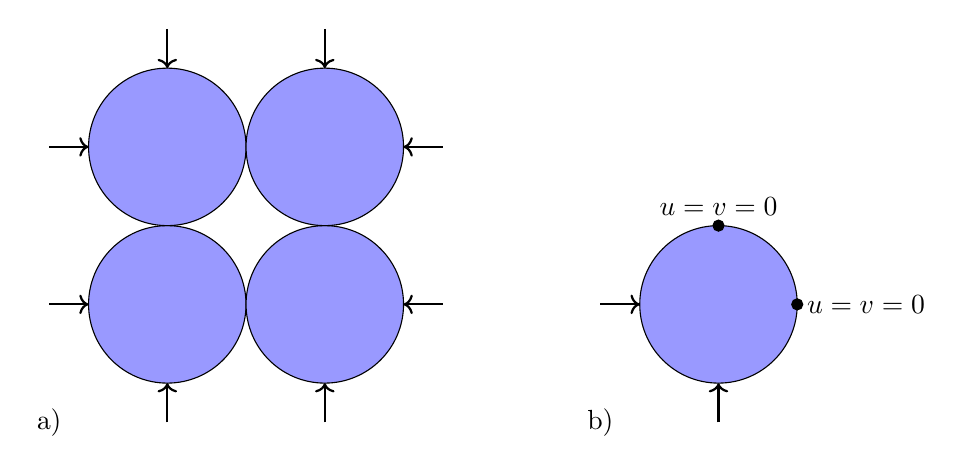
\begin{tikzpicture}
%\draw[fill=gray!23,gray!23](0,0) rectangle (11,6);
%\draw[step=0.5cm,gray,very thin] (0,0) grid (11,6); %background grid
\filldraw[fill=blue!40!white, draw=black] (2,2) circle (1cm);
\filldraw[fill=blue!40!white, draw=black] (4,2) circle (1cm);
\filldraw[fill=blue!40!white, draw=black] (2,4) circle (1cm);
\filldraw[fill=blue!40!white, draw=black] (4,4) circle (1cm);
\draw[thick,->] (0.5,2) -- (1,2); \draw[thick,->] (5.5,2) -- (5,2);
\draw[thick,->] (0.5,4) -- (1,4); \draw[thick,->] (5.5,4) -- (5,4);
\draw[thick,->] (2,0.5) -- (2,1); \draw[thick,->] (2,5.5) -- (2,5);
\draw[thick,->] (4,0.5) -- (4,1); \draw[thick,->] (4,5.5) -- (4,5);
\draw[thick,->] (7.5,2) -- (8,2);
\draw[thick,->] (9,0.5) -- (9,1); 
\filldraw[fill=blue!40!white, draw=black] (9,2) circle (1cm);
\filldraw[black] (10,2) circle (2pt) node[anchor=west] {$u=v=0$};
\filldraw[black] (9,3) circle (2pt) node[anchor=south] {$u=v=0$};
\node[] at (0.5,0.5)   {a)};
\node[] at (7.5,0.5)   {b)};
\end{tikzpicture}\\
{\captionfont a) assembly of four circular grains and the pressure boundary conditions; 
b) simplified setup of a single grain.}
\end{center}

\begin{center}
\includegraphics[width=5.5cm]{python_codes/fieldstone_58/experiment2/displ}
\includegraphics[width=5.5cm]{python_codes/fieldstone_58/experiment2/displx}
\includegraphics[width=5.5cm]{python_codes/fieldstone_58/experiment2/disply}\\
\includegraphics[width=5.5cm]{python_codes/fieldstone_58/experiment2/divv}
\includegraphics[width=5.5cm]{python_codes/fieldstone_58/experiment2/p}
\includegraphics[width=5.5cm]{python_codes/fieldstone_58/experiment2/strain}\\
\includegraphics[width=10cm]{python_codes/fieldstone_58/experiment2/dispvect}
\end{center}



\noindent \Literature:
\begin{itemize}
\item Compaction creep of sands due to time-dependent grain failure: Effects of chemical environment,
      applied stress, and grain size. Brzesowsky \etal{} (2014) \cite{brhb14}
\item Failure behavior of single sand grains: Theory versus experiment. Brzesowsky \etal{} (2011) \cite{brsp11}
\item Time-independent compaction behavior of quartz sands. Brzesowsky \etal{} (2014) \cite{brsp14}
\item Determination of the tensile strength of rock by a compression test of an 
      irregular test piece. Hiramatsu \etal{} (1966) \cite{hiok66}
\item Micromechanics of sand grain failure and sand compaction. Brzesowsky (1995) \cite{brze95}
\item Contact fatigue in silica sand—Observations and modeling. Wang \& Michalowski (2015) \cite{wami15}
\item Tensile stress concentration and compressive failure in cemented granular material. 
      Wong \& Wu (1995)\cite{wowu95}
\item Micromechanics of pressure-induced grain crushing in porous rocks. Zhang \etal{} (1990) \cite{zhwd90}
\end{itemize}




 %%%%%%%%%%%%%%%%%%%%%%%%%%%%%%%%%%%%%%%%%%%%%%%%%%%%%%%%%%%%%%%%%%%%%%

\chapter{Ice Flow Down an Inclined Plane \label{f59}} %%%%%%%%%%%%%%%%%%%%%%%%%%%%%%%%%%%%%%%%%%%%%%%%%%%%%%%% 59

\includegraphics[height=1.5cm]{images/pictograms/replication}
\includegraphics[height=1.5cm]{images/pictograms/ice}

\begin{flushright} {\tiny {\color{gray} python\_codes/fieldstone\_59/text.tex}} \end{flushright}

\lstinputlisting[language=bash,basicstyle=\small]{python_codes/fieldstone_59/keywords.key}

\begin{center}
\fbox{\textbf{\huge \color{teal} P}}
Code at \url{https://github.com/cedrict/fieldstone/tree/master/python_codes/fieldstone_59}
\end{center}

\par\noindent\rule{\textwidth}{0.4pt}

%%%%%%%%%%%%%%%%%%%%%%%%%%%%%%%%%%%%%%%%%%%%%%%%%%%%%%%%%%%%%%%%%%%%%%%%%%%%%%%%%%%%%%%%%%%%%%%%%%%




\begin{center}
\includegraphics[width=5cm]{python_codes/fieldstone_59/images/setup}\\
{\captionfont REDO with tikz}
\end{center}

\paragraph{Linear viscous fluid}

We start from the Stokes equation for isoviscous fluids:
\[
\eta \Delta \vec{\upnu} - \vec\nabla p + \rho \vec{g} = \vec{0}
\]
Assuming that the fluid is incompressible and that the incline is infinite, 
then $\vec{\upnu}=(u(y),0)$.
The $x$-component of the equation then writes:
\[
\eta\left(\frac{\partial^2 u}{\partial x^2}+\frac{\partial^2 u}{\partial y^2} \right)
- \frac{\partial p}{\partial x} + \rho g_x =0
\]
\[
\Rightarrow \qquad 
\eta\frac{\partial^2 u}{\partial y^2} 
+ \rho g \sin\alpha =0
\]
since $\partial_x\rightarrow 0$.
This 2nd order ODE can be integrated twice. The two integration constants are 
determined by setting $u(y=0)=0$ (no slip) and the shear stress to be zero at the (free)
surface. The velocity profile is given by:
\[
u(y)=\frac{\rho g \sin \alpha}{2 \eta} (2h-y)y
\]
We can now compute the components of the strain rate tensor:
\[
\dot{\varepsilon}_{xx}=0
\qquad
\qquad
\dot{\varepsilon}_{yy}=0
\qquad
\qquad
\dot{\varepsilon}_{xy}
=\frac{1}{2} \left( \frac{\partial u}{\partial y} + \frac{\partial v}{\partial x} \right)
=\frac{1}{2} \frac{\partial u}{\partial y} 
= \frac{\rho g \sin \alpha}{2 \eta} (h-y)
\]

We now make the assumption that this problem is a very simplified ice sheet flow problem.
The angle $\alpha$ is typically small and for $\alpha\sim 0.5-1$\degree, then $\sin\alpha\sim 0.01$. 
We also have $\rho\sim1000$, $g\sim$10,  $h\sim2500$ and we postulate the 
ice viscosity to be $\eta\sim 10^m$,.
The velocity is maximum at the surface and is given by
\begin{equation}
u(y=h)=
\frac{\rho g \sin \alpha}{2 \eta}h^2 
\sim \frac{1000 \cdot 10 \cdot 0.01}{ 2\cdot 10^m}2500^2
\sim 3\cdot 10^{8-m}
\label{eq:ice1}
\end{equation}

\begin{center}
\includegraphics[height=9cm]{python_codes/fieldstone_59/images/neem}
\includegraphics[height=9cm]{python_codes/fieldstone_59/images/narh15}\\
{\captionfont Ice velocity map (magnitude, in logarithmic scale) of the Greenland Ice Sheet
derived from SAR data of the Sentinel-1A satellite, acquired in Interferometric Wide Swath
Mode (IW) between January and March 2015. Taken from \textcite{narh15} (2015).}
\end{center}

As shown on the figures above the typical ice sheet velocity values around the NEEM ice core 
is $\sim 0.03~\si{\meter\per\day} \simeq 3\cdot 10^{-7}~\si{\meter\per\second}$. 
Then, in order for the top of the ice sheet to flow at this speed it requires $m=15$.

Having obtained the (effective linear) viscosity of the ice, i.e. 
$\eta\simeq 10^{15}~\si{\pascal\second}$,
we can compute the strain rate at the bottom and in the middle:
\[
\dot{\varepsilon}_{xy}(y=0) 
= \frac{\rho g \sin \alpha}{2 \eta} h
\sim \frac{1000\cdot 10 \cdot 0.01}{2 \cdot 10^{15}}2500
\sim 10^{-10}~\si{\per\second}
\]
\[
\dot{\varepsilon}_{xy}(y=h/2) 
= \frac{\rho g \sin \alpha}{2 \eta} \frac{h}{2}
\sim \frac{1000\cdot 10 \cdot 0.01}{2 \cdot 10^{15}}\frac{2500}{2}
\sim 5\cdot 10^{-11}~\si{\per\second}
\]
which are reasonable values as confirmed by the following figure (see yellow line):  
\begin{center}
\includegraphics[width=11cm]{python_codes/fieldstone_59/images/kudd19}\\
{\captionfont Taken from \textcite{kudd19} (2019).}
\end{center}

The conclusion from this exercise is that {\sl if} ice could be described by 
a linear viscous fluid flowing on an infinite incline, a viscosity of $\eta\simeq 10^{15}$Pa.s
would yield observations that match recorded velocities and strain rates. 


\paragraph{Nonlinear power-law viscosity}
However, the picture is way more complex, as it was observed very early on 
by Glen in 1955 \cite{glen55} and many others later (see Section~\ref{MMM-ss:glen}). 
It was then found that the strain rate and the stress are linked in a nonlinear way: 
\[
\dot{\varepsilon} = A \tau^n,
\]
i.e. the ice behaves as a power-law fluid (see Section~\ref{MMM-ss:powerlaw}), with 
$n=3$ and $A\simeq 2.4\cdot 10^{-24}$ at 0\degree (REF?).

More recently \textcite{kuwd19} (2019) and \textcite{kudd19} (2019) derived a composite flow law 
to model deformation in the NEEM deep ice core. 
They start from the flow law proposed by \textcite{goko01} (2001):
\[
\dot{\varepsilon}_T = \dot{\varepsilon}_{disl} + 
\left(\frac{1}{ \dot{\varepsilon}_{basal}} + \frac{1}{ \dot{\varepsilon}_{GBS}} \right)^{-1} 
+  \dot{\varepsilon}_{diff}
\]
where $\dot{\varepsilon}_T$  is the total strain rate, 
composed of strain rates for basal slip accommodated by non-basal slip or dislocation creep,
$\dot{\varepsilon}_{disl}$ , grain boundary sliding (GBS) accommodated by basal slip, 
$\dot{\varepsilon}_{basal}$ , and basal slip accommodated by GBS, 
$\dot{\varepsilon}_{GBS}$ , and diffusion creep, 
$\dot{\varepsilon}_{diff}$. Each of these creep mechanisms can be described by a 
power law relation of the form:
\[
\dot{\varepsilon} = A \tau^n d^{-p} \exp \left( -\frac{Q+pV}{RT} \right)
\]
where $A$ is a material parameter, $\tau$ is the differential stress (MPa), 
$n$ is the stress exponent, $d$ is the grain size diameter (\si{\meter}), 
$p$ is the grain size exponent, $Q$ is the activation energy for the creep 
mechanism at stake ($\si{\joule\per\mole}$), $p$ is the hydrostatic pressure ($\si{\mega\pascal}$), 
$V$ the activation volume ($\si{\cubic\meter\per\mole}$), 
$R$ is the gas constant ($\si{\joule\per\kelvin\per\mole}$), 
and $T$ the absolute temperature ($\si{\kelvin}$). 
The effect of $pV$ is assumed to be very small \cite{dust01} 
and is ignored for the remainder of this work.

As explained in \textcite{kuwd19} (2019) the composite flow law can actually be simplified to:
\[
\dot{\varepsilon}_T = \dot{\varepsilon}_{disl} + \dot{\varepsilon}_{GBS}
\]
The material parameters for these deformation mechanisms are available in \cite{kudd19}:
\begin{center}
\begin{tabular}{lcccc}
\hline
Creep regime & $A$ & $n$ & $p$ & $Q$ (\si{\joule\per\mole}) \\
\hline\hline
Glen's flow law ($T<263$K) &$3.61\cdot10^5$ MPa$^{-3.0}$ s$^{-1}$ &3.0 &0 &60\\
Glen's flow law ($T>263$K) &$1.73\cdot10^{21}$ MPa$^{-3.0}$ s$^{-1}$ &3.0 &0 &139\\
\hline
Dislocation creep ($T<262$K) & $5.0\cdot10^5$ MPa$^{-4.0}$ s$^{-1}$ &4.0 &0 &64\\
Dislocation creep ($T>262$K) &$6.96\cdot 10^{23}$ MPa$^{-4.0}$ s$^{-1}$ &4.0 &0 &155\\
\hline
GBS-limited creep ($T<262$K) & $1.1\cdot 10^2$ MPa$^{-1.8}$ m$^{1.4}$ $s^{-1}$ &1.8 &1.4 &70\\
GBS-limited creep ($T>262$K) & $8.5\cdot10^{37}$ MPa$^{-1.8}$ m$^{1.4}$ $s^{-1}$ &1.8 &1.4 &250\\
\hline
\end{tabular}
\end{center}

The associated effective viscosity is then given by 
\[
\eta = \frac{1}{2}  A^{-\frac{1}{n}} \dot{\varepsilon}^{\frac{1}{n}-1}  d^{\frac{p}{n}} \exp \left( \frac{Q+pV}{nRT} \right)
\]
Note that the $A$ parameter is given in MPa and not Pa so that when computing the 
associated effective viscosities these have to be multiplied by $10^6$.
Because the strain rates are added together we know that the two deformation mechanisms are in series and their
effective viscosity is then the harmonic average of both viscosities:
\[
\eta_{eff} = \left(\frac{1}{\eta_{disl}} + \frac{1}{\eta_{GBS}}  \right)^{-1}
\]

\paragraph{Numerical setup}

The geometry is a 2D cartesian domain of size $L_x \times L_y$. Instead of tilting it by an angle $\alpha$
I choose to instead 'tilt' the gravity vector so that it becomes 
$\vec{g}=(\rho g \sin\alpha,-\rho g\cos\alpha)$.
The boundary conditions are as follows: no slip at the bottom, free surface at the top, 
free slip on the left (we assume that this corresponds to a ridge - zero horizontal velocity)
and we need to be careful about the right boundary which is where the ice exits the domain:
if we leave the boundary open ice will rush out, generate high strain rates and the nonlinear 
rheologies will respond by generating low viscosities which in turn will promote a fast 
exit. Instead we opt to prescribe the analytical solution of Eq.~(\ref{MMM-eq:ice1}) with $\eta=10^{15}$.
We neglect any kind of phase change and precipitation and only carry out a single time step.
The domain is discretised with nel=nelx$\times$nely $Q_2Q_1$ elements (see Section~\ref{MMM-ss:pairq2q1}).
We set $L_x=125$km and $L_y=2500$m, $\rho=917$kg$\cdot$m$^{-3}$, $\alpha=0.1$\degree.



\begin{center}
\includegraphics[width=7cm]{python_codes/fieldstone_59/images/shsh14}
\includegraphics[width=10cm]{python_codes/fieldstone_59/images/kuiper19}\\
{\captionfont Left: Taken from \textcite{shsh14} (2014); 
Right: Taken from \textcite{kuiper19} (2019).}
\end{center}

I have obtained the raw data (curtesy from E.N. Kuiper) and it is plotted hereunder:
\begin{center}
\includegraphics[width=8cm]{python_codes/fieldstone_59/data/temperature}
\includegraphics[width=8cm]{python_codes/fieldstone_59/data/grain_size}
\end{center}

In order to verify that the values reported in the table above are the ones 
used in \cite{kudd19} I have reproduced the figure 3 of that paper (code and gnuplot
script in {\sl ./data} folder):
\begin{center}
\includegraphics[width=9cm]{python_codes/fieldstone_59/data/strainrate}\\
{\captionfont Log strain rate versus temperature for Glen's flow law and 
the two mechanisms (dislocation creep and GBS-limited creep) that form the end members 
of the modified composite flow law, using the flow law parameters from the table above. 
A stress of 0.07MPa and a mean grain diameter of $5~\si{\milli\meter}$ 
were used to calculate the strain rate.}
\end{center}


In our models, the temperature profile is simplified 
as shown on the plots above. 
Concerning the grain size distribution the ice sheet has been divided in three 
layers and and an average grain size is used for each.

We have computed the effective viscosity for all four rheologies with the 
implemented temperature and grain size profiles for $\dot{\varepsilon}_e=10^{-10}\text{s}^{-1}$:

\begin{center}
\includegraphics[width=8cm]{python_codes/fieldstone_59/results/profiles}
\includegraphics[width=8cm]{python_codes/fieldstone_59/results/profiles2}
\end{center}
Note that smaller strain rates shift the curves to the right (higher viscosities).



Because the rheologies are non linear we need to carry out nonlinear iterations 
(see Section~\ref{MMM-ss:picard}).
In what follows we run models for Glen's flow law (rheology=1), 
dislocation creep (rheology=2), GBS (rheology=3) and dislocation+GBS (rheology=4).
Note that in the case of rheology=4, the partitioning of the strain rates between both 
mechanisms is not done (YET) so that the results are not really consistent with the rest!

%\newpage
\begin{center}
Core 1 ($x=L_x/4$) \hspace{5cm}  Core 2 ($x=L_x/2$)  \\
\includegraphics[width=7.cm]{python_codes/fieldstone_59/results/u_core1}
\includegraphics[width=7.cm]{python_codes/fieldstone_59/results/u_core2}\\
\includegraphics[width=7.cm]{python_codes/fieldstone_59/results/sr_core1}
\includegraphics[width=7.cm]{python_codes/fieldstone_59/results/sr_core2}\\
\includegraphics[width=7.cm]{python_codes/fieldstone_59/results/eta_core1}
\includegraphics[width=7.cm]{python_codes/fieldstone_59/results/eta_core2}\\
\includegraphics[width=7.cm]{python_codes/fieldstone_59/results/sigmaxx_core1}
\includegraphics[width=7.cm]{python_codes/fieldstone_59/results/sigmaxx_core2}\\
\includegraphics[width=7.cm]{python_codes/fieldstone_59/results/sigmayy_core1}
\includegraphics[width=7.cm]{python_codes/fieldstone_59/results/sigmayy_core2}\\
\includegraphics[width=7.cm]{python_codes/fieldstone_59/results/sigmaxy_core1}
\includegraphics[width=7.cm]{python_codes/fieldstone_59/results/sigmaxy_core2}
\end{center}


\begin{center}
\includegraphics[width=7cm]{python_codes/fieldstone_59/results/rh4/vel}
\includegraphics[width=7cm]{python_codes/fieldstone_59/results/rh4/p}\\
\includegraphics[width=7cm]{python_codes/fieldstone_59/results/rh4/sr}
\includegraphics[width=7cm]{python_codes/fieldstone_59/results/rh4/eta}\\
{\captionfont Velocity, pressure, strain rate and effective viscosity in the middle of the ice sheet
for rheology=4}
\end{center}



Check: ELMER/ice \url{http://elmerice.elmerfem.org/capabilities}

Improvements: better density profile? more realistic geometry ? 
partitioning of strain rates. Better temperature profile. 
Better grain size description. Influence of tilt angle? 

\vspace{1cm}

\Literature 
\textcite{buja89} (1989),
\textcite{zwgg07} (2007),
\textcite{zhjg11} (2011),
\textcite{lejx14} (2014),
\textcite{issg15} (2015),
\textcite{yash15} (2015),
\textcite{gors17} (2017),
\textcite{heah18} (2018).


 %%%%%%%%%%%%%%%%%%%%%%%%%%%%%%%%%%%%%%%%%%%%%%%%%%%%%%%%%%%%%%%%%%%%%%

\chapter{DG-FEM: 1D advection \label{f60}} %%%%%%%%%%%%%%%%%%%%%%%%%%%%%%%%%%%%%%%%%%%%%%%%%%%%%%%%%%%%%%%%%%% 60 
\lstinputlisting[language=bash,basicstyle=\small]{python_codes/fieldstone_60/keywords.ascii}

This stone implements the 1D discontinuous Galerkin method to solve the simple 
advection equation:
\[
\frac{\partial T}{\partial t} + u \frac{\partial T}{\partial x} = 0
\]




%---------------------------------------------
\subsection*{The code}

The mesh counts {\tt nelx} linear elements and therefore {\tt nnx} nodes.

The timestep is determined by means of the CFL condition:
\begin{lstlisting}
dt=C*hx/u
\end{lstlisting}
The mesh is very simply built:
\begin{lstlisting}
x=np.linspace(0,Lx,nnx)
\end{lstlisting}
We need to declare four arrays: the nodal temperature both on the left and 
on the right of each node, and their memory of the previous time step. 
\begin{lstlisting}
T_minus=np.zeros(nnx,dtype=np.float64)      
T_minus_old=np.zeros(nnx,dtype=np.float64)  
T_plus=np.zeros(nnx,dtype=np.float64)       
T_plus_old=np.zeros(nnx,dtype=np.float64)   
\end{lstlisting}
Initial temperatures are then prescribed on both {\tt T\_plus} 
and $T\_minus$ arrays, and then copied to the 'old' arrays.

We then enter the time stepping loop:
\begin{lstlisting}
for istep in range(0,nstep):
\end{lstlisting}
At each timestep the boundary conditions are reapplied\footnote{It is a bit weird that 
we prescribe a temperature b.c. on a node with an outflow...?}:
\begin{lstlisting}
T_minus[0]=T_left
T_plus[0]=T_left
T_minus[nnx-1]=T_right
T_plus[nnx-1]=T_right
\end{lstlisting}
We then loop over all elements:
\begin{lstlisting}
for iel in range(0,nel):
\end{lstlisting}
and compute the corresponding $k$ and $k+1$ values:
\begin{lstlisting}
k=iel
kp1=iel+1
\end{lstlisting}
The $T^+$ and $T^-$ fields are then updated following Eq.~\eqref{eq:dgadv5}:
\begin{lstlisting}
T_plus[k]   =T_plus_old[k]   +C*(-3*T_plus_old[k]-T_minus_old[k+1]+4*T_minus[k])
T_minus[k+1]=T_minus_old[k+1]+C*( 3*T_plus_old[k]-T_minus_old[k+1]-2*T_minus[k])
\end{lstlisting}







%---------------------------------------------
\subsection*{Results}

%---------------------------------------------
\subsubsection*{Experiment 1}

We consider the following advection problem taken from Li \cite[ex 5.2]{li06}.
It is also carried out in \stone~43.

The domain has dimension $L_x=1$. 
The temperature is prescribed on the left and the right boundary to be zero. 
The initial temperature is given by
\[
T(x,0)=
\left\{
\begin{array}{ll}
\sin (10 \pi x) & \textrm{for } x< 0.1 \\
0               & \textrm{for } x\geq 0.1 
\end{array}
\right.
\]
The velocity is set to $u=0.1$.
We use 200 elements and a time step of $\delta t=10^{-4}$. 
We run the model to time $t=8$ so we need 80,000 time stpes. 

Note that the CFL-number is then very small: 
\[
C = \frac{\delta t \cdot u}{h} = \frac{10^{-4} \cdot  0.1}{1/200} = 0.002
\]

\begin{center}
\includegraphics[width=9cm]{python_codes/fieldstone_60/results/exp1/T.pdf}\\
{\captionfont Temperature field at three different times.}
\end{center}

\todo[inline]{redo with standard Galerkin and compare!}

%---------------------------------------------
\subsubsection*{Experiment 2}

This advection benchmark originates in Donea \& Huerta \cite{dohu03}
and it also to be found in Thieulot (2011) \cite{thie11} (and in 
Section~\ref{ss:appAthie11}).

The domain has dimension $L_x=1$. 
The temperature is prescribed on the left at $T=1$
and the right boundary at $T=0$.
The initial temperature is given by
\[
T(x,0)=
\left\{
\begin{array}{ll}
1 & \textrm{for } x< 0.25 \\
0 & \textrm{for } x\geq 0.1 
\end{array}
\right.
\]
Velocity is set to $u=1$, the number of elements to 50 ($h=0.02$), the CFL number to 0.1 (
so $\delta t=0.002$), and the number of time steps to 250, so that we expect the front
to be at $x=3L_x/4$.  

\begin{center}
\includegraphics[width=8cm]{python_codes/fieldstone_60/results/exp2/T.pdf}\\
\includegraphics[width=8cm]{images/supg/fantom3}\\
{\captionfont Left: Temperature field at different times; 
Right: Taken and modified from Thieulot (2011) \cite{thie11}}
\end{center}

It is rather surprising that the DG results are so much worse than the SG results (even without 
SUPG stabilisation).









 %%%%%%%%%%%%%%%%%%%%%%%%%%%%%%%%%%%%%%%%%%%%%%%%%%%%%%%%%%%%%%%%%%%%%%

\chapter{Channel flow with Herschel-Bulkley rheology \label{f61}} %%%%%%%%%%%%%%%%%%%%%%%%%%%%%%%%%%%%%%%%%%%% 61
\includegraphics[height=1.25cm]{images/pictograms/benchmark}
\includegraphics[height=1.25cm]{images/pictograms/FEM}

%%%%%%%%%%%%%%%%%%%%%%%%%%%%%%%%%%%%%%%%%%%%%%%%%%%%%%%%%%%%%%%%%%%%%%%%%%%%%%%%%%%%%%%%%%%%%%%%%%%

\lstinputlisting[language=bash,basicstyle=\small]{python_codes/fieldstone_61/keywords.ascii}

\begin{center}
Code at \url{https://github.com/cedrict/fieldstone/tree/master/python_codes/fieldstone_61}
\end{center}

\par\noindent\rule{\textwidth}{0.4pt}
%%%%%%%%%%%%%%%%%%%%%%%%%%%%%%%%%%%%%%%%%%%%%%%%%%%%%%%%%%%%%%%%%%%%%%%%%%%%%%%%%%%%%%%%%%%%

\paragraph{Simple Newtonian Poiseuille flow} The analytical solution to this flow has been derived 
in Section~\ref{MMM-ss:poiseuille}.
We set $p_{left}=10^9$, $p_{right}=0$, $L_x=L_y=100$km, $\eta_0=10^{25}$, so 
\[
\Pi=\frac{p_{right}-p_{left}}{L_x}=-10^4 <0
\]
The $p_{left}$ value is prescribed on the left (see Section~\ref{MMM-ss:openbc}) while 
nothing is prescribed on the right. No slip boundary conditions are 
prescribed on the top and bottom.

We see that we recover the analytical solution for velocity and strainrate:
\begin{center}
\includegraphics[width=7.8cm]{python_codes/fieldstone_61/results/poiseuille/velocity}
\includegraphics[width=7.8cm]{python_codes/fieldstone_61/results/poiseuille/exy}
\end{center}

\begin{center}
\includegraphics[width=5cm]{python_codes/fieldstone_61/results/poiseuille/vel}
\includegraphics[width=5cm]{python_codes/fieldstone_61/results/poiseuille/press}
\includegraphics[width=5cm]{python_codes/fieldstone_61/results/poiseuille/sr}
\end{center}

\paragraph{Poiseuille flow with H-B rheology - $n=1$} 
The analytical solution to this flow has been derived in Section~\ref{MMM-ss:HBflow}.
In this case we have 
\[
\eta_{HB}
=
\left\{
\begin{array}{lc}
\eta_0 & \dot{\varepsilon}_e\leq \dot{\varepsilon}_0 \\
K  + \frac{\tau_0}{\dot{\varepsilon}_e}  
& \dot{\varepsilon}_e\geq \dot{\varepsilon}_0 
\end{array}
\right.
\]
and the limiting viscosity $\eta_0$ is such that 
\[
\eta_0 = K  + \frac{\tau_0}{\dot{\varepsilon}_0}  
\]

\begin{center}
\includegraphics[width=7.8cm]{python_codes/fieldstone_61/results/n_1/velocity.pdf}
\includegraphics[width=7.8cm]{python_codes/fieldstone_61/results/n_1/exy.pdf}\\
\includegraphics[width=7.8cm]{python_codes/fieldstone_61/results/n_1/eta.pdf}
\includegraphics[width=7.8cm]{python_codes/fieldstone_61/results/n_1/press.pdf}\\
\includegraphics[width=7.8cm]{python_codes/fieldstone_61/results/n_1/nonlinear_conv.pdf}
\end{center}

\begin{center}
\includegraphics[width=7.8cm]{python_codes/fieldstone_61/results/n_1/vel.png}
\includegraphics[width=7.8cm]{python_codes/fieldstone_61/results/n_1/exy.png}\\
\includegraphics[width=7.8cm]{python_codes/fieldstone_61/results/n_1/eta.png}
\includegraphics[width=7.8cm]{python_codes/fieldstone_61/results/n_1/press.png}
\end{center}





 %%%%%%%%%%%%%%%%%%%%%%%%%%%%%%%%%%%%%%%%%%%%%%%%%%%%%%%%%%%%%%%%%%%%%% 

\chapter{Subduction a la Quinquis Case 1 \label{f62}} %%%%%%%%%%%%%%%%%%%%%%%%%%%%%%%%%%%%%%%%%%%%%%%%%%%%%%%% 62
\includegraphics[height=1.25cm]{images/pictograms/replication}
\includegraphics[height=1.25cm]{images/pictograms/benchmark}
\includegraphics[height=1.25cm]{images/pictograms/triangle}
\includegraphics[height=1.25cm]{images/pictograms/under_construction}
\includegraphics[height=1.25cm]{images/pictograms/FEM}
\includegraphics[height=1.25cm]{images/pictograms/paraview}

%%%%%%%%%%%%%%%%%%%%%%%%%%%%%%%%%%%%%%%%%%%%%%%%%%%%%%%%%%%%%%%%%%%%%%%%%%%%%%%%%%%%%%%%%%%%%%%%%%%


\lstinputlisting[language=bash,basicstyle=\small]{python_codes/fieldstone_62/keywords.ascii}

\begin{center}
Code at \url{https://github.com/cedrict/fieldstone/tree/master/python_codes/fieldstone_62}
\end{center}

\par\noindent\rule{\textwidth}{0.4pt}
%%%%%%%%%%%%%%%%%%%%%%%%%%%%%%%%%%%%%%%%%%%%%%%%%%%%%%%%%%%%%%%%%%%%%%%%%%%%%%%%%%%%%%%%%%%%

The setup is presented in the phd thesis (chapter 4) of M. Quinquis \cite{quin14},
In this stone we focus on the case 1 of his work and only solve the system once (single time step).
The domain is $1500\times 670$ km. 

The setup and the boundary conditions are shown hereunder:
\begin{center}
\includegraphics[width=\linewidth]{python_codes/fieldstone_62/images/quin14_setup}\\
{\captionfont Model setup for subduction of a 70 Ma old oceanic plate under a 40 Ma
old oceanic plate. A) Setup of the whole model. The top, bottom, and left boundaries
are free-slip, while the right boundary condition includes material in- and outflow. S HB :
Serpentinised Harzburgite, and B OC : Bulk Oceanic Composition. The ‘thermal’ layers
are only required in the linear viscous models. B) Zoom of the setup at the trench, h is the
thickness of the weak zone. C) Definition of the in- and outflow velocities on the right
boundary. Taken from \cite{quin14}}
\end{center}

As opposed to the original benchmarking effort carried out by Quinquis and collaborators
I build the mesh with triangles so that I can exactly represent the layers (and especially 
the weak zone) with an adequate resolution. The elements used are the Crouzeix-Raviart one
(see Section~\ref{MMM-sec:crouzeix-raviart}). 

In {points.py} the coordinates of the key points are defined. The {generate\_nodes.py}
script generates the input file for 
the {\sl triangle} program\footnote{\url{https://www.cs.cmu.edu/~quake/triangle.html}}. 
Finally the {fieldstone.py} script 
reads in the mesh, sets up the material layout, the boundary conditions and solves the 
FE system. Simply use the {\sl run} script to trigger the mesh generation and the FE 
calculations.  
Note that the compiled {\sl triangle} executable file (as compiled by you 
on your own machine) must be present in this folder.

\begin{center}
\includegraphics[width=\linewidth]{python_codes/fieldstone_62/results/mats1}\\
{\captionfont Taken from \cite{quin14}}
\end{center}

The letters referenced in the {points.py} file are shown hereunder:

\begin{center}
\includegraphics[width=11cm]{python_codes/fieldstone_62/images/setup1}\\
\includegraphics[width=11cm]{python_codes/fieldstone_62/images/setup2}
\end{center}


In this case 1, all materials are characterised by a constant density and a Newtonian rheology:
\begin{center}
\includegraphics[width=5cm]{python_codes/fieldstone_62/images/quin14_mats}
\end{center}

\newpage
\begin{center}
\includegraphics[width=13cm]{python_codes/fieldstone_62/results/mesh1}\\
\includegraphics[width=13cm]{python_codes/fieldstone_62/results/mesh2}\\
\includegraphics[width=13cm]{python_codes/fieldstone_62/results/mesh3}
\end{center}

\newpage
\begin{center}
\includegraphics[width=12.5cm]{python_codes/fieldstone_62/results/density}\\
\includegraphics[width=12.5cm]{python_codes/fieldstone_62/results/viscosity}\\
\includegraphics[width=12.5cm]{python_codes/fieldstone_62/results/velocity}\\
\includegraphics[width=12.5cm]{python_codes/fieldstone_62/results/u}\\
\includegraphics[width=12.5cm]{python_codes/fieldstone_62/results/v}\\
\end{center}

\newpage
\begin{center}
\includegraphics[width=10cm]{python_codes/fieldstone_62/results/vel2}\\
\includegraphics[width=10cm]{python_codes/fieldstone_62/results/vel3}\\
\includegraphics[width=10cm]{python_codes/fieldstone_62/results/vel4}
\end{center}

I believe that one source of our problems when we carried out resolution tests
came from the fact that this small convection cell that occurs as shown above was
always under-resolved. The top layer is 8km thick and the weak zone is 14km thick,
and we ran simulations at max 1km resolution. However, because of the use  
of particle-in-cell and rectangular elements (mostly linear elements), 
a proper capture of this feature in the solution would have required much higher 
resolution. In other words, our higher resolution runs were probably not high resolution enough.
Given the nature of this convection cell, it means that temperature would be advected by it, 
and that markers would likely gotten mixed. 

\newpage
\begin{center}
\includegraphics[width=13cm]{python_codes/fieldstone_62/results/sr1}\\
\includegraphics[width=13cm]{python_codes/fieldstone_62/results/sr2}
\end{center}



 %%%%%%%%%%%%%%%%%%%%%%%%%%%%%%%%%%%%%%%%%%%%%%%%%%%%%%%%%%%%%%%%%%%%%%

\chapter{failure in cemented granular material \label{f63}} %%%%%%%%%%%%%%%%%%%%%%%%%%%%%%%%%%%%%%%%%%%%%%%%%% 63 

\includegraphics[width=1.5cm]{images/pictograms/replication}

\lstinputlisting[language=bash,basicstyle=\small]{python_codes/fieldstone_63/keywords.ascii}

\par\noindent\rule{\textwidth}{0.4pt}

{\sl This stone was developed in collaboration with Taka Shinohara}.
\index{contributors}{Taka Shinohara}

\par\noindent\rule{\textwidth}{0.4pt}

%%%%%%%%%%%%%%%%%%%%%%%%%%%%%%%%%%%%%%%%%%%%%%%%%%%%%%%%%%%%%%%%%%%%%%%%%%%%%%%%%%%%%%%%

This \stone is based on \textcite{wowu95} (1995) published in Geophysical Research Letters. 
As for every \stone aiming at reproducing results off a publication I here include de abstract
of the article:

\begin{center}
\begin{minipage}{13cm}
{\small 
Grain crushing and pore collapse are important micromechanical processes responsible for hydrostatic and 
shear-enhanced compactions in porous rocks. These processes initiate from extensile microcracks which 
emanate from grain contacts. Microstructural observations indicate that such extensile cracking is inhibited 
in the vicinity of cemented grain contacts. The finite element technique was used to simulate the tensile 
stress concentration and normal stiffness in a cemented aggregate. The detrital grains were assumed to 
be elastically identical spheres bonded by cement layers of finite thickness. The numerical simulations 
show that the maximum tensile stress concentration is located near the triple junction (among grain, 
cement and pore space), and its magnitude is significantly less than that for an uncemented system. 
The development of microcracking near a cemented contact is readily inhibited unless the applied 
stress exceeds a critical value which is at least an order of magnitude greater than that for the 
onset of Hertzian fracture.
}
\end{minipage}
\end{center}

In this paper the authors use the finite element method to simulate 
the tensile stress concentration and normal stiffness in a cemented
aggregate. The grains are assumed to be elastically identical spheres
bonded by cement layers of finite thickness.

\begin{center}
\includegraphics[width=8cm]{python_codes/fieldstone_63/images/yoyo}
\includegraphics[width=6cm]{python_codes/fieldstone_63/images/domain}\\
{\captionfont Left: model of cemented granular system for 
axisymmetric finite element analysis (taken from \cite{wowu95}); Right: 
Domain for a\_fac=0.2 and h\_fac=5/90 and $R=90\mu m$.}
\end{center}

We define
\[
a_{fac} = \frac{a}{R}  
\qquad
\text{and}
\qquad 
h_{fac} = \frac{h}{R}
\]
which translates as follows in the code:
\begin{lstlisting}
outer_radius=90e-6      #radius R (m)  
a_fac = 20/90           # ratio of a to R 
h_fac = 5/90            # ratio of h to R
a = outer_radius*a_fac
h = outer_radius*h_fac
\end{lstlisting}

The material properties for the grain and the cement are as follows:

\begin{lstlisting}
#Quartz mechanical properties
E1 = 95e9                       # Young's modulus (Pa)
nu1=0.08                        # poisson ratio
mu1= E1/(2*(1+nu1))             # shear modulus
lambdaa1=2.*mu1*nu1/(1.-2.*nu1)  
\end{lstlisting}
and
\begin{lstlisting}
#cement mechanical properties 2 
E2 = 84e9                       # Young's modulus (Pa)
nu2=0.31                        # poisson ratio
mu2= E2/(2*(1+nu2))             # shear modulus
lambdaa2=2.*mu2*nu2/(1.-2.*nu2)  
\end{lstlisting}

Note that since gravitational effects are neglected we set $\vec{g}=\vec{0}$
so that density actually play no role in the model.

The mesh in the code is built in three phases: first, the quarter grain is meshed 
with triangles. Second, the cement block is meshed and shaped so as to follow the 
shape of the grain. Finally both meshes are merged together:

\begin{center}
\includegraphics[width=5.5cm]{python_codes/fieldstone_63/images/wowu95b}
\includegraphics[width=8cm]{python_codes/fieldstone_63/images/mesh}\\
{\captionfont Left: quadtree-based mesh used in \cite{wowu95}; 
Right: low resolution fieldstone mesh.}
\end{center}

Boundary conditions are as follows: $u=0$ is prescribed on the left and top boundary, 
while $v=0$ is prescribed on the bottom boundary, as shown below.
Additionally, traction b.c. are prescribed at the top\footnote{Note that 
in the axisymmetric case these then apply onto a disc and should be multiplied by $2\pi$} (these
are described in Section~\ref{MMM-ss:openbc}) as indicated hereunder:
\begin{center}
a)\includegraphics[width=5cm]{python_codes/fieldstone_63/images/bc_u}
b)\includegraphics[width=5cm]{python_codes/fieldstone_63/images/bc_v}\\
c)\includegraphics[width=4cm]{python_codes/fieldstone_63/images/wowu95}\\
{\captionfont a,b) Horizontal and vertical displacement boundary condition indicator.
c) Imposed traction at the top surface (Taken from \cite{wowu95}).}
\end{center}

Linear triangular elements are used and a 3-point numerical quadrature is used.
Average elemental quantities are computed with 7 quadrature points.
These same quantities are also projected onto the nodes for visualisation purposes.
Principal stresses are computed as explained in Section~\ref{MMM-sec:princ_stress}.

The code solves the FE system and retrieves the deformation components $x$ and $y$,
or $r$ and $z$ in the axisymmetric case.
Average elemental strain components are then computed. In the axisymmetric case
then  $\varepsilon_{\theta\theta}$ is computed and otherwise set to zero in the plane strain case.
The stress tensor components are then computed as follows:
\begin{eqnarray}
\sigma_{xx} &=& \lambda \vec\nabla\cdot\vec{u} + 2\mu \varepsilon_{xx} \\
\sigma_{zz} &=& \lambda \vec\nabla\cdot\vec{u} + 2\mu \varepsilon_{zz} \\
\sigma_{xz} &=&  2\mu \varepsilon_{xz} 
\end{eqnarray}
where $\vec\nabla\cdot\vec{u}=\frac{\partial u}{\partial x} + \frac{\partial w}{\partial z}$
in plane strain and 
$\vec\nabla\cdot\vec{u}=\frac{\partial u}{\partial x} + \frac{u}{x} + \frac{\partial w}{\partial z}$
in the axisymmetric case\footnote{Remember that the $xz$ plane is in fact the $rz$ plane so that 
the term $u_r/r$ becomes $u/x$ in practice.}.

Principal stresses are such that $\sigma_1>\sigma_2$ and 
\[
\sigma_{1,2}=\frac{\sigma_{xx}+\sigma_{yy}}{2} 
\pm \sqrt{  \left(\frac{\sigma_{xx}-\sigma_{yy}}{2}\right)^2 +\sigma_{xy}^2 }
 \]
The principal direction angle $\theta_p$ defines the principal
directions where the only stresses are normal stresses, and 
is given by the relationship:
\[
\tan (2\theta_p) =  \frac{2 \sigma_{xy}}{\sigma_{xx} -\sigma_{yy}}
\]
We find that $\theta_2$ is always negative, while $\theta_1$ showcases positive and negative values. 
We define the tensile zone as $\sigma_1>0$.

In general $\sigma_1$ is the maximum (most tensile) principal stress, 
$\sigma_3$ is the minimum (most compressive) principal stress, 
and $\sigma_2$ is the intermediate principal stress.

The maximum shear stress (in 2D) is given by
\[
\tau_{max} = \frac12(\sigma_1-\sigma_2)
\]

In the axisymmetric case the stress tensor is given by 
\[
{\bm \sigma} = 
\left(
\begin{array}{ccc}
\sigma_{rr} & 0 & \sigma_{rz} \\
0 & \sigma_{\theta\theta} & 0 \\
\sigma_{rz} & 0 & \sigma_{zz} 
\end{array}
\right)
\]
There are now three eigenvalues. However it is obvious that $\sigma_{\theta\theta}$ is 
one of them and the other two correspond to those of the $2\times 2$ stress stensor with 
$\sigma_{rr}$, $\sigma_{rz}$ and $\sigma_{zz}$ terms.
The code therefore needs not be modified to compute these. 



\begin{center}
\includegraphics[width=8.5cm]{python_codes/fieldstone_63/images/wowu95c}\\
{\captionfont Contours for the minimum principal stress in the vicinity of the triple junction}
\end{center}

\begin{remark}
This paper by Wong and Wu is a nice example of not-reproducible science. For one, boundary conditions 
are not all specified. Second, it is not specified whether the results are obtained in plane strain 
or axisymmetric geometry. Third, the program that was used is proprietary (ABAQUS). 
Fourth, no resolution tests are presented: given how small the area A is, and how comparable 
in size it is to the elements, this is problematic. Fifth, it is not clear how the 
tensile zone is defined. Sixth: the type of finite element is not specified. Seven, 
we are shown one field which is a derivative of the solution (displacement) but not the 
solution itelf.  
\end{remark}

The following results are obtained with very high resolutions, i.e. 
nLayers=901, nel\_h=80. This yields a mesh with about 1.6M triangles, 
and Nfem=1,668,488.

\newpage
%-----------------------------------------------------------------------
\paragraph{Results in plane strain}


\begin{center}
\includegraphics[width=5.5cm]{python_codes/fieldstone_63/results/ps/disp}
\includegraphics[width=5.5cm]{python_codes/fieldstone_63/results/ps/disp_x}
\includegraphics[width=5.5cm]{python_codes/fieldstone_63/results/ps/disp_y}\\
\includegraphics[width=5.5cm]{python_codes/fieldstone_63/results/ps/sigma1}
\includegraphics[width=5.5cm]{python_codes/fieldstone_63/results/ps/sigma2}
\includegraphics[width=5.5cm]{python_codes/fieldstone_63/results/ps/strain}\\
\includegraphics[width=5.5cm]{python_codes/fieldstone_63/results/ps/angle}
\includegraphics[width=5.5cm]{python_codes/fieldstone_63/results/ps/maximum_shear_stress}
\includegraphics[width=5.5cm]{python_codes/fieldstone_63/results/ps/tensile}
\end{center}

\newpage
%-----------------------------------------------------------------------
\paragraph{Results in axisymmetric geometry}

\begin{center}
\includegraphics[width=5.5cm]{python_codes/fieldstone_63/results/axi/disp}
\includegraphics[width=5.5cm]{python_codes/fieldstone_63/results/axi/disp_x}
\includegraphics[width=5.5cm]{python_codes/fieldstone_63/results/axi/disp_y}\\
\includegraphics[width=5.5cm]{python_codes/fieldstone_63/results/axi/sigma1}
\includegraphics[width=5.5cm]{python_codes/fieldstone_63/results/axi/sigma2}
\includegraphics[width=5.5cm]{python_codes/fieldstone_63/results/axi/strain}\\
\includegraphics[width=5.5cm]{python_codes/fieldstone_63/results/axi/angle}
\includegraphics[width=5.5cm]{python_codes/fieldstone_63/results/axi/maximum_shear_stress}
\includegraphics[width=5.5cm]{python_codes/fieldstone_63/results/axi/tensile}
\end{center}

 %%%%%%%%%%%%%%%%%%%%%%%%%%%%%%%%%%%%%%%%%%%%%%%%%%%%%%%%%%%%%%%%%%%%%%

\chapter{Elasto-viscous benchmarks \label{f64}} %%%%%%%%%%%%%%%%%%%%%%%%%%%%%%%%%%%%%%%%%%%%%%%%%%%%%%%%%%%%%% 64
\lstinputlisting[language=bash,basicstyle=\small]{python_codes/fieldstone_64/keywords.ascii}

\begin{center}
Code at \url{https://github.com/cedrict/fieldstone/tree/master/python_codes/fieldstone_64}
\end{center}

\par\noindent\rule{\textwidth}{0.4pt}
%%%%%%%%%%%%%%%%%%%%%%%%%%%%%%%%%%%%%%%%%%%%%%%%%%%%%%%%%%%%%%%%%%%%%%%%%%%%%%%%%%%%%%%%%%%%


{\large
DO NOT READ WHAT FOLLOWS. It was written for Composition based stone, but I am using 
markers for all benchmarks so far. Jump directly to 'stress build up in maxwell body'! 
}

In the examples here there are only 2 compositions. 
Each material/composition is characterised by its $\eta_{\{1,2\}}$, $\mu_{\{1,2\}}$. 
With $\delta t$ chosen, $Z_{\{1,2\}}$ and $\eta_{eff,\{1,2\}}$ can be computed.

C1 and C2 are initialised at startup by looping over Vnodes and assigning a value to $C_1$ 
and $C_2$ such that $C_1+C_2=1$. 

The quantity $\tau_{xx},\tau_{yy},\tau_{xy},\dot{\omega}_{xy}$ (denoted by oxy in the code) 
are nodal and initialised at startup
(they are needed for the Stokes matrix):
\begin{lstlisting}
tauxx =np.zeros(NV,dtype=np.float64)  
tauyy =np.zeros(NV,dtype=np.float64)  
tauxy =np.zeros(NV,dtype=np.float64)  
oxy   =np.zeros(NV,dtype=np.float64)  
etaeff=np.zeros(NV,dtype=np.float64)  
Z     =np.zeros(NV,dtype=np.float64)  
rho   =np.zeros(NV,dtype=np.float64)  
\end{lstlisting}

Structure of the code (the following bulletpoints are inside the time stepping loop):

\begin{itemize}
\item Nodal $\eta_{eff}$, $Z$ and $\rho$ values are computed as follows:
\begin{lstlisting}
for i in range(0,NV):
    etaeff[i]=C1[i]*etaeff1+C2[i]*etaeff2
    Z[i]     =C1[i]*Z1     +C2[i]*Z2
    rho[i]   =C1[i]*rho1   +C2[i]*rho2
\end{lstlisting}

\item Build Stokes matrix. 
Loop over elements, loop over integration points inside the element, and for 
each quadrature point:
\begin{eqnarray}
Z(\vec{r}_q) &=& \sum_{i=1}^{m_V} N_i^\upnu(\vec{r}_q) Z_i \\
\tau_{xx}(\vec{r}_q)&=& \sum_{i=1}^{m_V} N_i^\upnu(\vec{r}_q) \tau_{xx,i} \\
\tau_{yy}(\vec{r}_q)&=& \sum_{i=1}^{m_V} N_i^\upnu(\vec{r}_q) \tau_{yy,i} \\
\tau_{xy}(\vec{r}_q)&=& \sum_{i=1}^{m_V} N_i^\upnu(\vec{r}_q) \tau_{xy,i} \\
\eta_{eff}(\vec{r}_q)&=& \sum_{i=1}^{m_V} N_i^\upnu(\vec{r}_q) \eta_{eff,i} \\
\dot{\omega}_{xy}(\vec{r}_q) &=& \sum_{i=1}^{m_V} N_i^\upnu(\vec{r}_q)  \dot{\omega}_{xy,i} \\
\rho(\vec{r}_q) &=& \sum_{i=1}^{m_V} N_i^\upnu(\vec{r}_q) \rho_i 
\end{eqnarray}


The elastic memory rhs term is built following Eq.~(\ref{XXX}):
\begin{lstlisting}
R[0]=Zq*(tauxxq+dt*oxyq*(2*tauxyq))
R[1]=Zq*(tauyyq+dt*oxyq*(-2*tauxyq))
R[2]=Zq*(tauxyq+dt*oxyq*(tauyyq-tauxxq))
f_el-=b_mat.T.dot(R)*weightq*jcob
\end{lstlisting}

\item Solve system and obtain $u,v,p$

\item Compute nodal velocity gradient ${\bm L}=\vec\nabla\vec\upnu$

\item Compute derivated nodal fields 

\begin{lstlisting}
exx[:]=Lxx[:]
eyy[:]=Lyy[:]
exy[:]=0.5*(Lxy[:]+Lyx[:])
oxy[:]=0.5*(Lxy[:]-Lyx[:])
Jxx[:]=2*tauxx[:]*oxy[:]
Jyy[:]=-2*tauxy[:]*oxy[:]
Jxy[:]=(tauyy[:]-tauxx[:])*oxy[:]
\end{lstlisting}

\item (re-)build nodal ${\bm \tau}$: 
\begin{lstlisting}
tauxx=2*etaeff*exx+Z*tauxx+Z*dt*Jxx
tauyy=2*etaeff*eyy+Z*tauyy+Z*dt*Jyy
tauxy=2*etaeff*exy+Z*tauxy+Z*dt*Jxy
\end{lstlisting}

\item advect $C_1$, $C_2$, $\tau_{xx}$, $\tau_{yy}$ and $\tau_{xy}$ fields

\item produce vtu file

\end{itemize}





%.......................................................
\paragraph{About this code}

This is a fairly complicated code since it features a deformable mesh 
(by means of a simplified ALE which only allows for the vertical movement 
of only the top row of mesh nodes), a particle-in-cell technique (only 
1st order in space)
to carry out material tracking/advection and of course the elasto-viscous 
rheology.


%.......................................................
\paragraph{Stress build-up in viscoelastic Maxwell body - analytical solution}

We start from 
\[
\dot{\bm \varepsilon}_T = \dot{\bm \varepsilon}_e +\dot{\bm \varepsilon}_v
=\frac{1}{2\mu} \dot{\bm \tau} + \frac{1}{2\eta} {\bm \tau} 
\]
In the case where there is no rotation then the BLABLA derivative becomes $d/dt$
and then 
we have to solve 
\[
2 \mu \dot{\bm \varepsilon}_T 
= \frac{d {\bm \tau}}{dt} + \frac{\mu}{\eta} {\bm \tau}
= \frac{d {\bm \tau}}{dt} + \frac{{\bm \tau}}{t_M}
\]
where $t_M=\eta/mu$ is the Maxwell time. The general solution can be arrived at 
by means of the Laplace transform (?!) and is given by:
\[
{\bm \tau}(t) = {\bm \tau}(t_0) \exp\left( -\frac{t-t_0}{t_M} \right) + \exp \left(-\frac{t}{t_M}\right)
\int_{t_0}^{t} 2 \mu \dot{\bm \varepsilon}_T  \exp \left(\frac{t'}{t_M}\right) dt'
\]

If $t_0=$ and ${\bm \tau}(t_0)=0$ then
\[
{\bm \tau}(t) =  \exp \left(-\frac{t}{t_M}\right)
\int_{0}^{t} 2 \mu \dot{\bm \varepsilon}_T  \exp \left( \frac{t'}{t_M} \right) dt'
\]
If the strain rate and shear modulus are constant in time, then 
\begin{eqnarray}
{\bm \tau}(t) 
&=&  \exp \left(-\frac{t}{t_M}\right)
2 \mu \dot{\bm \varepsilon}_T   \int_{0}^{t} \exp \left( \frac{t'}{t_M} \right) dt' \nn\\
&=&  \exp \left(-\frac{t}{t_M}\right)
2 \mu \dot{\bm \varepsilon}_T  t_M  \left[ \exp \left( \frac{t}{t_M} \right) -1  \right] \nn\\
&=& 
2 \eta \dot{\bm \varepsilon}_T   \left[ 1 - \exp \left( -\frac{t}{t_M} \right)\right] \nn
\end{eqnarray}
since $t_M=\eta/\mu$.

%.......................................................
\paragraph{Stress build-up in viscoelastic Maxwell body under simple shear}

The first benchmark performed to test the viscoelastic implementation considers the stress 
build-up present in a viscoelastic Maxwell body. Contrary to stressed viscous materials, 
viscoelastic materials gradually build-up stress when sheared after which a transition to viscous deformation occurs.  

An unstressed, incompressible viscoelastic Maxwell medium is subjected to a velocity field 
resulting in pure shear. 
The increase of the accumulated stress with time is given by an analytical solution:
\begin{equation}
{\bm \tau} = 2\eta\ {\dot{\bm \varepsilon}} \left ( 1-e^{-\frac{\mu }{\eta} t } \right )
\end{equation}
with $t$ time, $\eta$ the prescribed material viscosity and $\mu$ the prescribed material shear modulus. 
The domain size is 100$\times 100$km.
The velocity prescribed at all boundaries equals $v=1$ cm/yr in magnitude yielding a constant 
background strain rate of $\dot{\varepsilon}=2\text{cm/yr}/100\text{km}\simeq 6.342\times 10^{-15}$. 
The viscosity is $\eta= 10^{21}\text{Pa.s}$, the shear modulus is 
$\mu =10^{10}$Pa and the gravity is set to zero. We set $\delta t=100$yr.  

\begin{center}
\includegraphics[width=5cm]{python_codes/fieldstone_64/images/stress_buildup_setup.png}\\
\captionfont{
Set up of the stress build-up benchmark. All domain sides have a free slip
boundary condition, and pure shear velocity conditions are prescribed. Adapted from 
Gerya (2010) \cite{gery10}.} 
\end{center}

We have 
\[
\eta_{eff} 
= \frac{\eta \delta t}{\delta t + \eta/\mu} 
= \frac{10^{21} \cdot 3.154\times 10^{9}}{3.154\times 10^{9} + 10^{21}/10^{10}} 
\simeq 
3.0592 \times 10^{19}\text{Pa.s}
\qquad
\text{and}
\qquad
Z=\frac{\eta_{eff}}{\mu \delta t} 
\simeq 
0.9694
\]
The Maxwell time is $t_M = \frac{\eta}{\mu} = 10^{11}\text{s} \simeq 3171\text{yr}$.
In the absence of elasticity (purely viscous behaviour), we have 
$\dot{\varepsilon}_{xx} = 6.342\times 10^{-15}$ 
and $\eta=10^{21}$ so the 
deviatoric stress $\tau_{xx}$ is equal to 
\[
\tau_{xx} = 2 \cdot 10^{21} \cdot 6.342\times 10^{-15} \simeq 12.68 \times 10^6 \text{Pa}
\]

The first time that the Stokes system is solved, there is no stored stress, i.e. the 
elastic rhs is identically zero, so that the system is solved with a viscosity equal to
$\eta_{eff}$.
We can easily compute the analytical solution, and we see that $\dot{\varepsilon}_{xy}=0$
and $\dot{\omega}_{xy}=0$, which we recover:

\begin{center}
\includegraphics[width=5cm]{python_codes/fieldstone_64/results/buildup_11/init/vel}
\includegraphics[width=5cm]{python_codes/fieldstone_64/results/buildup_11/init/exy}
\includegraphics[width=5cm]{python_codes/fieldstone_64/results/buildup_11/init/oxy}
\end{center}

The expected stress value for $\tau_{xx}$ after the first Stokes solve is 
\[
\tau_{xx} = 2 \eta_{eff} \dot{\varepsilon}_{xx} 
= 2 \cdot 3.057\times 10^{19} \cdot 6.342\times 10^{-15} 
\simeq 38.775 \times 10^4 \text{Pa}
\]

\begin{center}
\includegraphics[width=9cm]{python_codes/fieldstone_64/results/buildup_11/tauxx}\\
{\captionfont $\tau_{xx}$ as a function of time.}
\end{center}

\includegraphics[width=5cm]{python_codes/fieldstone_64/results/buildup_11/tau}
\includegraphics[width=5cm]{python_codes/fieldstone_64/results/buildup_11/strainrate}
\includegraphics[width=5cm]{python_codes/fieldstone_64/results/buildup_11/velocity}\\

\begin{remark}
Because of the outflux boundary conditions it can happen that some markers 
exit the domain. In order to avoid dealing with these, markers are artificially 
kept inside the domain (near the boundary).
\end{remark}

%.......................................................
\paragraph{Stress build-up in viscoelastic Maxwell body under simple shear}

I have also created a similar problem, although this time simple shear boundary conditions are prescribed.
$v=0$ on left and right boundary, (-1,0)cm/yr at the bottom, (+1,0)cm/yr at the top.

ANALYTICAL SOLUTION!?!
$\tau_{xy} \rightarrow 2 \eta \dot{\varepsilon}_xy = 6.342\times 10^{6} Pa$ 

\begin{center}
\includegraphics[width=5cm]{python_codes/fieldstone_64/results/buildup_12/vel}
\end{center}

In simple shear, we have $\dot{\varepsilon}_{xx}=\dot{\varepsilon}_{yy}=0$, and 
\[
\dot{\varepsilon}_{xy}=\frac{1}{2} \frac{\Delta u}{L_y} = \frac{1 cm/yr}{100km}
\]

\begin{center}
\includegraphics[width=9cm]{python_codes/fieldstone_64/results/buildup_12/tauxy}\\
{\captionfont $\tau_{xy}$ as a function of time.}
\end{center}

\includegraphics[width=5cm]{python_codes/fieldstone_64/results/buildup_12/tau}
\includegraphics[width=5cm]{python_codes/fieldstone_64/results/buildup_12/strainrate}
\includegraphics[width=5cm]{python_codes/fieldstone_64/results/buildup_12/velocity}\\




%........................
\paragraph{Bending of elastic slab}

The sinking slab benchmark consists of a beam of elastic material which is placed 
in a weak and viscous surrounding medium. The initially unstressed beam is attached 
to the left domain boundary through boundary conditions. A stress is then applied to 
the beam in the form of gravity. The applied gravity force results in the deformation 
of the beam through bending. After 20 kyr, the gravity field is turned off and the 
elastic properties of the beam will then force itself to its original position.  
The set-up of the benchmark is given in the following figure: 

\begin{center}
\includegraphics[width=6cm]{python_codes/fieldstone_64/images/poster_benchmark.png}\\
\captionfont{Set-up of the benchmark from \cite{gery10}. The properties of the 
two materials are given on the left, together\\ with the initial configuration of the benchmark.} 
\end{center}

The beam is surrounded by a low-density, low-viscosity and high shear modulus medium 
of which the specifications are given in  the following table.
The boundary conditions of the domain consist of a no slip condition at 
the left boundary where the slab is attached and free slip boundary conditions along all other sides. 
The results are calculated on a grid with a resolution of 50x50 elements containing 64 randomly 
distributed markers at startup.
The time step is set to $\delta t = 200yr$ (i.e. gravity is switched off after 100 time steps).

\begin{center}
\begin{tabular}{lll}
\hline 
\textit{Material properties}& \textit{Elastic slab (fluid 1)}  & \textit{Surrounding medium (fluid 2)} \\
\hline 
\hline 
Density         $\rho$ \     [kg/m$^{3}$]      & 4000                    & 1     \\
Viscosity       $\eta$ \    [Pa$\cdot$ s]      & $10^{27}$               &   $10^{21}$     \\
Shear modulus   $\mu $ \    [Pa]               & $10^{10}$               & $10^{20}$       \\
Maxwell time $t_M$     \    [yr]               & 3.17Gyr                 &  $3.17\times10^{-7}$yr       \\
eff. visc.      $\eta_{eff}$ \ [Pa$\cdot$s]    & 6.307199602192306e+19   &  9.999999984145105e+20      \\
visco-elasticity factor $Z$      \ [-]         & 0.9999999369280039      &  1.5854895966744522e-09     \\
\hline 
\end{tabular} 
\end{center}

\begin{center}
\includegraphics[height=4.5cm]{python_codes/fieldstone_64/images/gerya1}
\includegraphics[height=4.5cm]{python_codes/fieldstone_64/images/gerya2}
\includegraphics[height=4.5cm]{python_codes/fieldstone_64/images/gerya3}\\
\includegraphics[height=4.5cm]{python_codes/fieldstone_64/results/slab/markers0000}
\includegraphics[height=4.5cm]{python_codes/fieldstone_64/results/slab/markers0100}\\
{\captionfont Top row taken from \cite[16.11]{gery10}. 
Results of a numerical experiment for the recovery of the original
shape of a visco-elastic slab (black, dark grey), 
 embedded in a weak visco-elastic medium (light grey, white). 
(a) Initial configuration, (b) configuration after 20 Kyr of deformation under 
constant vertical gravity field ($g_x=0$,$g_y =-10\text{m/s}^2$, 
(c) configuration achieved within 9980 Kyr of spontaneous deformation after 
switching off gravity (i.e. after $g_x=g_z=0$ condition is applied at
20 Kyr). Numerical results are calculated at a resolution 51$\times$51 nodes and
200$\times$200 markers. Note the irreversible viscous deformation of the weak surrounding medium,
which is visible in its perturbed checkerboard structure close to slab corners in (c).}
\end{center}

\newpage
The first time that the Stokes system is solved, there is no stored stress, i.e. the 
elastic rhs is identically zero, and the system is solved with a viscosity equal to
$\eta_{eff,1}$ and $\eta_{eff,2}$ for the slab and mantle respectively:

\begin{center}
\includegraphics[width=5.2cm]{python_codes/fieldstone_64/results/slab/init/vel}
\includegraphics[width=5.2cm]{python_codes/fieldstone_64/results/slab/init/u}
\includegraphics[width=5.2cm]{python_codes/fieldstone_64/results/slab/init/v}\\
\includegraphics[width=5.2cm]{python_codes/fieldstone_64/results/slab/init/exx}
\includegraphics[width=5.2cm]{python_codes/fieldstone_64/results/slab/init/eyy}
\includegraphics[width=5.2cm]{python_codes/fieldstone_64/results/slab/init/exy}\\
\includegraphics[width=5.2cm]{python_codes/fieldstone_64/results/slab/init/q}
\includegraphics[width=5.2cm]{python_codes/fieldstone_64/results/slab/init/etaeff}
\includegraphics[width=5.2cm]{python_codes/fieldstone_64/results/slab/init/rho}
\end{center}

Note that the Gerya data are obtained with the code from the 2010 version of the book.

\begin{center}
\includegraphics[width=7cm]{python_codes/fieldstone_64/results/slab/velocity_u}
\includegraphics[width=7cm]{python_codes/fieldstone_64/results/slab/velocity_v}\\
\includegraphics[width=7cm]{python_codes/fieldstone_64/results/slab/J}
\includegraphics[width=7cm]{python_codes/fieldstone_64/results/slab/tau}
\end{center}


\newpage

\begin{center}
\includegraphics[width=5cm]{python_codes/fieldstone_64/results/slab/gerya2/markers_0000_Myr}
\includegraphics[width=5cm]{python_codes/fieldstone_64/results/slab/gerya2/stress_0000_Myr}
\includegraphics[width=5cm]{python_codes/fieldstone_64/results/slab/gerya2/velocity_0000_Myr}\\
\includegraphics[width=5cm]{python_codes/fieldstone_64/results/slab/gerya2/markers_0010_Myr}
\includegraphics[width=5cm]{python_codes/fieldstone_64/results/slab/gerya2/stress_0010_Myr}
\includegraphics[width=5cm]{python_codes/fieldstone_64/results/slab/gerya2/velocity_0010_Myr}\\
\includegraphics[width=5cm]{python_codes/fieldstone_64/results/slab/gerya2/markers_0020_Myr}
\includegraphics[width=5cm]{python_codes/fieldstone_64/results/slab/gerya2/stress_0020_Myr}
\includegraphics[width=5cm]{python_codes/fieldstone_64/results/slab/gerya2/velocity_0020_Myr}\\
\includegraphics[width=5cm]{python_codes/fieldstone_64/results/slab/gerya2/markers_0030_Myr}
\includegraphics[width=5cm]{python_codes/fieldstone_64/results/slab/gerya2/stress_0030_Myr}
\includegraphics[width=5cm]{python_codes/fieldstone_64/results/slab/gerya2/velocity_0030_Myr}\\
\includegraphics[width=5cm]{python_codes/fieldstone_64/results/slab/gerya2/markers_0040_Myr}
\includegraphics[width=5cm]{python_codes/fieldstone_64/results/slab/gerya2/stress_0040_Myr}
\includegraphics[width=5cm]{python_codes/fieldstone_64/results/slab/gerya2/velocity_0040_Myr}\\
\includegraphics[width=5cm]{python_codes/fieldstone_64/results/slab/gerya2/markers_0100_Myr}
\includegraphics[width=5cm]{python_codes/fieldstone_64/results/slab/gerya2/stress_0100_Myr}
\includegraphics[width=5cm]{python_codes/fieldstone_64/results/slab/gerya2/velocity_0100_Myr}\\
{\captionfont Results obtained with the Matlab code provided with Gerya (2019) \cite{gery19book}}
\end{center}

\newpage
%.......................................................
\paragraph{Stress build-up in viscoelastic Maxwell body}

This benchmark comes from Appendix B of Keller et al (2013) \cite{kemk13}.

The domain is $7.5\times5$km. A dominantly elastic beam is fixed to, and protrudes horizontally 
from the left wall of the model box. 
Surrounding the elastic beam is a viscous, but inelastic fluid. 
All boundaries are free slip, except for the left wall, which is set to no slip in 
order to keep the bending beam fixed to the wall. The beam has a higher density than the surrounding fluid and
thus will bend down elastically driven by gravity. After the beam has 
accumulated some elastic strain through bending down, gravity is switched off. 
If the stress evolution is implemented accurately, the elastic beam should now, 
free from the pull of gravity, move upwards again and restore its initial position. 

Material properties are as follows:
\begin{itemize}
\item beam: $\rho=1500$, $\eta=10^{24}$, $\mu=10^{10}$
\item fluid: $\rho=1000$, $\eta=10^{18}$, $\mu=10^{11}$
\end{itemize}

This choice of parameters leads to a Maxwell time 
$t_m = 0.32$ yr for the background fluid and Maxwell times of 
$t_m = 3.2$ Myr for the beam, meaning that the deformation in this benchmark problem, 
which occurs on a timescale of thousands to a million years, 
will lead to dominantly viscous deformation in the fluid, 
and dominantly elastic behaviour of the beam. 

Keller et al set the numerical resolution to $300\times200$ elements, 
with 16 markers per elements for stress advection. Such a resolution is 
not feasible with our simple python implementation so the resolution is
then set to $96\times64$. 

The following plot comes from \cite{kemk13}:
\begin{center}
\includegraphics[width=14cm]{python_codes/fieldstone_64/images/kemk13}
\end{center}

The elastic timestep is set to $\delta t_e=100$yr and the tectonic timestep is set to the same value.
This yields $\eta_{eff}=10^{18}$ in the fluid, and $\eta_{eff}\simeq 3.15\times 10^{19}$.
After 50kyr, the gravity ($|\vec{g}|=10$) is switched off and the model is ran for another 
500kyr.


\begin{center}
\includegraphics[width=5cm]{python_codes/fieldstone_64/results/beam/u.png}
\includegraphics[width=5cm]{python_codes/fieldstone_64/results/beam/v.png}
\includegraphics[width=5cm]{python_codes/fieldstone_64/results/beam/vel}\\
\includegraphics[width=5cm]{python_codes/fieldstone_64/results/beam/exx}
\includegraphics[width=5cm]{python_codes/fieldstone_64/results/beam/eyy}
\includegraphics[width=5cm]{python_codes/fieldstone_64/results/beam/exy}\\
\includegraphics[width=5cm]{python_codes/fieldstone_64/results/beam/q}
\includegraphics[width=5cm]{python_codes/fieldstone_64/results/beam/rho}
\includegraphics[width=5cm]{python_codes/fieldstone_64/results/beam/Z}\\
{\captionfont Various fields at the end of the 1st timestep: 
Velocity, strain rate components, $Z$, $\eta_{eff}$, strain rate components, pressure.}
\end{center}

\begin{center}
\includegraphics[width=7cm]{python_codes/fieldstone_64/results/beam/u.pdf}
\includegraphics[width=7cm]{python_codes/fieldstone_64/results/beam/u_log.pdf}\\
\includegraphics[width=7cm]{python_codes/fieldstone_64/results/beam/v.pdf}
\includegraphics[width=7cm]{python_codes/fieldstone_64/results/beam/v_log.pdf}
\end{center}

\begin{center}
\includegraphics[width=5cm]{python_codes/fieldstone_64/results/beam/tauxx.pdf}
\includegraphics[width=5cm]{python_codes/fieldstone_64/results/beam/tauyy.pdf}
\includegraphics[width=5cm]{python_codes/fieldstone_64/results/beam/tauxy.pdf}
\end{center}


\newpage
%.......................................................
\paragraph{Flexure of elastic plate}

This benchmark is presented in Choi et al (2013) \cite{chtl13}. 
The setup is as follows:

\begin{center}
\includegraphics[width=12cm]{python_codes/fieldstone_64/images/chtl13a}
\end{center}

\begin{center}
\begin{tabular}{llll}
\hline 
\textit{Material properties}& \textit{elastic plate (1)}  & \textit{elastic block (2)} & \textit{viscous mantle (3)} \\
\hline 
\hline 
Density         $\rho$       \ [kg/m$^{3}$]       & 2700&1890 &2700 \\ 
Viscosity       $\eta$       \ [Pa$\cdot$ s]      & $10^{35}$& $10^{35}$ & $10^{17}$ \\ 
Shear modulus   $\mu $       \ [Pa]               & $30\cdot10^9$& $30\cdot10^9$&  $10^{50}$ \\
Maxwell time    $t_M$        \ [yr]               & 10569930 &  10569930 & 3.1709791983764584e-41 \\ 
eff. visc.      $\eta_{eff}$ \ [Pa$\cdot$s]       & 4.73039776e+18& 4.73039776e+18&  1e+17\\ 
Factor          $Z$          \ [-]                & 0.9999995&  0.9999995 &  6.3419583e-42 \\ 
\hline 
\end{tabular} 
\end{center}

The value of $\eta_1=\eta_2=10^{35}$ for the elastic materials was obtained through personal communication. 
The value of $\mu_3=10^{50}$ for the viscous material ensures that $\eta_{eff}=\eta_3$.
Note that in the publication the authors test both compressible and incompressible 
formulations, but we restrict ourselves to incompressible results since our code cannot handle compressible behavior. 
I also use dt=5year.

The authors report a converged total relief of 306-308m:

\begin{center}
\includegraphics[width=8cm]{python_codes/fieldstone_64/images/chtl13b}
\end{center}

This benchmark requires either a sticky air layer (see Section~\ref{sss:stickyair})
on top of the plate or a deformable mesh (ALE formulation, see Section~\ref{sss:ale}).


\begin{center}
\includegraphics[width=5cm]{python_codes/fieldstone_64/results/flexureplate/u.png}
\includegraphics[width=5cm]{python_codes/fieldstone_64/results/flexureplate/v.png}
\includegraphics[width=5cm]{python_codes/fieldstone_64/results/flexureplate/vel.png}\\
{\captionfont Initial velocity field}
\end{center}

On the following figures I plot the topography and velocity statistics obtained with 
a resolution of $100\times35$ elements and 50 markers per element, next to 
results from Choi et al and/or results with my code \elefant \cite{thie14}.  
\begin{center}
\includegraphics[width=5cm]{python_codes/fieldstone_64/results/flexureplate/topo.pdf}
\includegraphics[width=5cm]{python_codes/fieldstone_64/results/flexureplate/v.pdf}
\includegraphics[width=5cm]{python_codes/fieldstone_64/results/flexureplate/v_log.pdf}
\end{center}

\begin{center}
\includegraphics[width=5cm]{python_codes/fieldstone_64/results/flexureplate/tauxx}
\includegraphics[width=5cm]{python_codes/fieldstone_64/results/flexureplate/tauyy}
\includegraphics[width=5cm]{python_codes/fieldstone_64/results/flexureplate/tauxy}\\
{\captionfont accumulated deviatoric stress at time t=500yr on the markers.}
\end{center}


\begin{center}
\includegraphics[width=16cm]{python_codes/fieldstone_64/results/flexureplate/grid}\\
{\captionfont Grid at time t=500yr}
\end{center}


%The following figure shows the grid at equilibrium and the markers:

%\begin{center}
%\includegraphics[width=8cm]{FLEXTURE_OF_ELASTIC_PLATE/mats.png}
%\includegraphics[width=8cm]{FLEXTURE_OF_ELASTIC_PLATE/DevStressInv.png}\\
%\includegraphics[width=8cm]{FLEXTURE_OF_ELASTIC_PLATE/maxwelltime.png}
%\includegraphics[width=8cm]{FLEXTURE_OF_ELASTIC_PLATE/mu_ve}\
%\end{center}


\newpage
%.......................................................
\paragraph{Ice load}

The domain is $500\times500$km. Vertical gravity is 9.8, density is 3300, viscosity 
is $3\cdot10^{20}$, shear modulus is $10^{10}$, free slip on left, right and bottom. 
A normal stress is imposed on the top for $0<x<100$km. It corresponds to 
an ice sheet of density $\rho_i=900$ of 1000m height. 
The timestep is set to 100yr. Resolution is set to $50\times50$ elements.
Stress/traction b.c. are explained in Section~\ref{ss:openbc}.

Analytical solution is provided in Nakiboglu and Lambeck (1982) \cite{nala82}. 
Note however that this is a 2D setup while the original solution is for a 
cylindrical load and also for a semi-infinite domain.

\[
\eta_{eff} = \frac{\eta \delta t}{\delta t + \eta/\mu}
= 2.85362675546547e+19
\]

\begin{center}
\includegraphics[width=10cm]{python_codes/fieldstone_64/results/icesheetload/vel}\\
{\captionfont Left: ASPECT; Right: stone 64}
\end{center}


\begin{center}
\includegraphics[width=6cm]{python_codes/fieldstone_64/results/icesheetload/topo3}
\includegraphics[width=6cm]{python_codes/fieldstone_64/results/icesheetload/vel_stats}
\end{center}

\includegraphics[width=5cm]{python_codes/fieldstone_64/results/icesheetload/tauxx}
\includegraphics[width=5cm]{python_codes/fieldstone_64/results/icesheetload/tauyy}
\includegraphics[width=5cm]{python_codes/fieldstone_64/results/icesheetload/tauxy}
 %%%%%%%%%%%%%%%%%%%%%%%%%%%%%%%%%%%%%%%%%%%%%%%%%%%%%%%%%%%%%%%%%%%%%%

\chapter{steady-state advection-diffusion ($Q_1$) \label{f65}} %%%%%%%%%%%%%%%%%%%%%%%%%%%%%%%%%%%%%%%%%%%%%%% 65
\lstinputlisting[language=bash,basicstyle=\small]{python_codes/fieldstone_65/keywords.ascii}

\begin{center}
Code at \url{https://github.com/cedrict/fieldstone/tree/master/python_codes/fieldstone_65}
\end{center}

\par\noindent\rule{\textwidth}{0.4pt}
%%%%%%%%%%%%%%%%%%%%%%%%%%%%%%%%%%%%%%%%%%%%%%%%%%%%%%%%%%%%%%%%%%%%%%%%%%%%%%%%%%%%%%%%%%%%

Let us start by remembering that the Peclet number is given by 
\[
\Penb = \frac{uh}{2\kappa} = \frac{uh\rho C_p}{2 k}
\]
where $u$ is the velocity, $h$ is the element size and $\kappa$ is the diffusion coefficient.

%----------------------------
\subsection*{Experiment 1}
We wish to solve the advection-diffusion problem presented in 
Section~\ref{MMM-ss:advdiff}:
\begin{equation}
\rho C_p u \frac{dT}{dx} - k \frac{d^2T}{dx^2} = f \qquad \text{in} \quad [0,L_x]
\end{equation}
with the boundary conditions $T(x=0)=0$ and $T(x=L_x)=0$.

The domain is characterised by $L_x=1$, and since $L_y$ is irrelevant it is set to $L_x/10$.
We further set $nelx=10$, $f=1$, $\rho=1$, $C_p=1$, $u=1$.
We will consider three values of the Peclet number: 0.25, 1 and 5.
From these values we can compute the corresponding heat conductivity value $k$.
Linear elements are used.

The analytical solution is given by Eq.~(2.23) in Donea \& Huerta \cite{dohu03}:
\[
T(x)= \frac{f}{u_0} \left(  x - \frac{1-\exp(2x \; \Penb /h_x)}{1-\exp(2\; \Penb / h_x)} \right) 
\]

As $\Penb$ increases, a sharp gradient, sometimes called a boundary layer,
develops at the right end of the domain. For high $\Penb$ values, the solution shows 
spurious node to node oscillations, failing to capture the highly nonlinear change. This oscillatory
behavior is seen for $\Penb>1$ (see Donea \& Huerta \cite{dohu03}).

\begin{center}
\includegraphics[width=5.5cm]{python_codes/fieldstone_65/results/exp1/solution1.pdf}
\includegraphics[width=5.5cm]{python_codes/fieldstone_65/results/exp1/solution2.pdf}
\includegraphics[width=5.5cm]{python_codes/fieldstone_65/results/exp1/solution3.pdf}\\
\includegraphics[width=5.5cm]{python_codes/fieldstone_65/results/exp1/T1.pdf}
\includegraphics[width=5.5cm]{python_codes/fieldstone_65/results/exp1/T2.pdf}
\includegraphics[width=5.5cm]{python_codes/fieldstone_65/results/exp1/T3.pdf}\\
{\captionfont Left to right: $\Penb$=0.25, $Pe$=1, $Pe$=5}
\end{center}

Finally we see that we recover identical results as in Donea \& Huerta \cite{dohu03}:

\begin{center}
\includegraphics[width=8.6cm]{python_codes/fieldstone_65/images/dohu}
\end{center}

If we now use the artificial diffusion presented in Section~\ref{MMM-ss:supg}, we have
\[
\tilde{\kappa}=\beta \kappa \Penb = \beta \frac{k}{\rho C_p} \Penb
\]
with 
\[
\beta=\coth(\Penb)-\frac{1}{\Penb}
\]
which yields:
\[
\tilde{k} = \tilde{\kappa} \rho_0 C_p 
\]
and the code solves the following equation
\begin{equation}
\rho C_p u \frac{dT}{dx} - (k + \tilde{k})\frac{d^2T}{dx^2} = f \qquad \text{in} \quad [0,L_x]
\end{equation}


We observe that this approach recovers the analytical solution exactly:
\begin{center}
\includegraphics[width=5cm]{python_codes/fieldstone_65/results/exp1/artdiff/T1.pdf}
\includegraphics[width=5cm]{python_codes/fieldstone_65/results/exp1/artdiff/T2.pdf}
\includegraphics[width=5cm]{python_codes/fieldstone_65/results/exp1/artdiff/T3.pdf}\\
{\captionfont Left to right: $\Penb$=0.25, $\Penb$=1, $\Penb$=5}
\end{center}

If one now uses 'full upwinding', i.e. $\beta=1$, we see that the scheme is 
overly dissipative (i.e. overly diffusive):

\begin{center}
\includegraphics[width=5cm]{python_codes/fieldstone_65/results/exp1/artdiff1/T1.pdf}
\includegraphics[width=5cm]{python_codes/fieldstone_65/results/exp1/artdiff1/T2.pdf}
\includegraphics[width=5cm]{python_codes/fieldstone_65/results/exp1/artdiff1/T3.pdf}\\
{\captionfont Left to right: $\Penb$=0.25, $\Penb$=1, $\Penb$=5}
\end{center}

\paragraph{Pure diffusion} It is also worth noting that when the velocity $u=0$, then the ODE becomes 
\begin{equation}
- k \frac{d^2T}{dx^2} = f \qquad \text{in} \quad [0,L_x]
\end{equation}
and its solution is 
\[
T(x)=-\frac{k}{k} (\frac{1}{2}x^2 + a x + b)
\]
Using the boundary conditions $T(x=0)=0$ and $T(x=L_x)=0$, we find
\[
b=0
\qquad
a = Lx/2
\]
so the result is the following parabolic profile: 
\[
T(x)=\frac{f}{2k}x(L_x-x)
\]
with 
\[
q(x)=-\frac{dT}{dx} = -\frac{f}{k}x
\]


%..................................................................................
\subsection*{Experiment 2 - advection skew to the mesh}

The domain is a unit square. Resolution is $10\times10$ linear elements. Initial temperature is 
irrelevant since we compute the steady state field. 

\begin{center}
\includegraphics[width=7cm]{python_codes/fieldstone_65/images/setup}
\includegraphics[width=7cm]{python_codes/fieldstone_65/results/exp2/vel}\\
{\captionfont Left: Taken from Donea \& Huerta \cite{dohu03}. In our code we replace $u$ by the 
temperature $T$. Right: prescribed velocity field.}
\end{center}

\begin{remark}
On page 75 of \cite{dohu03} the authors state that 
"the diffusivity coefficient is taken to be $10^{-4}$ , 
corresponding to a mesh Peclet number of $10^4$. 
Given that $\Penb=u h/2\kappa$ and h=0.1, this statement makes no sense.
I have therefore chosen $\Penb=10^4$ and then 
$\kappa=uh/2\Penb = 5\cdot10^{-6}$.
\end{remark}

The norm of the velocity vector $\vec{\upnu}$ is $|\vec{\upnu}|=1$. 
Since the Peclet number is so high, we have 
\[
\tau = \frac{h}{2 u_0} \left( \coth (\Penb) -\frac{1}{\Penb} \right) \rightarrow 
\frac{h}{2 u_0} 
\]

We then conduct three experiments: one without stabilisation, one with (isotropic) artifical diffusion, and 
one with SUPG, from left to right on the following plots:

\begin{center}
\includegraphics[width=15cm]{python_codes/fieldstone_65/results/exp2/Temps2}\\
\includegraphics[width=15cm]{python_codes/fieldstone_65/results/exp2/Temps}\\
\includegraphics[width=15cm]{python_codes/fieldstone_65/images/exp2}\\
{\captionfont Left to right: Standard Galerkin method, artificial diffusion, SUPG. 
Bottom row taken from Donea \& Huerta \cite{dohu03}. }
\end{center}



%..................................................................................
\subsection*{Experiment 3 - DG book setup}

This setup comes from Li's book on Discontinuous Galerkin Methods \cite{li06}, Section 5.2.3.
The 2D advection-diffusion equation is solved on a unit square with the following boundary 
conditions:
\begin{itemize}
\item bottom: $T=0$
\item left: $T=0$ if $y>0.5$, $T=1$ otherwise
\item right: $T=0$
\item top: $\partial_y T=0$
\end{itemize} 
Note that is not clear which value is actually prescribed in the lower left corner. 

Coefficients are not specified but the experiment should be run at $u/\kappa=1,10,100$ where 
$D$ is the diffusion coefficient (in the book $D$ is used instead of $\kappa$).
We then set $\rho=C_p=1$, $u_0=1$ and we define $\xi=u/\kappa$ with $\xi=1,10,100$. Then 
\[
\Penb = \frac{h\xi}{2} 
\]
We finally set nelx=nely=32, so that the heat conductivity coefficient can be computed.


\begin{center}
\includegraphics[height=10cm]{python_codes/fieldstone_65/results/exp3/libook}
\includegraphics[height=10cm]{python_codes/fieldstone_65/results/exp3/Tnostab}\\
{\captionfont Left: Taken from Li \cite{li06}. Computed results for a 2-D convection-diffusion 
problem showing the effect of convection on the temperature distribution in the system.
Right: results obtained without any stabilisation. From top to bottom, $\Penb=0.015625$, 
$\Penb=0.15625$ and $\Penb=1.5625$.}
\end{center}

The code also automatically generates the following 3D plots, and we see that for $\xi=100$
we obtain a strong overshoot near the right boundary:

\begin{center}
\includegraphics[width=5cm]{python_codes/fieldstone_65/results/exp3/solution1.pdf}
\includegraphics[width=5cm]{python_codes/fieldstone_65/results/exp3/solution10.pdf}
\includegraphics[width=5cm]{python_codes/fieldstone_65/results/exp3/solution100.pdf}\\
{\captionfont No stabilisation, from left to right: $\xi=1,10,100$.}
\end{center}

If I now increase the resolution then $h$ becomes smaller and so does the Peclet number, so that 
the oscillations near the right wall disappear:

\begin{center}
\includegraphics[width=5cm]{python_codes/fieldstone_65/results/exp3/solution100.pdf}
\includegraphics[width=5cm]{python_codes/fieldstone_65/results/exp3/solution100_x2.pdf}
\includegraphics[width=5cm]{python_codes/fieldstone_65/results/exp3/solution100_x4.pdf}\\
{\captionfont No stabilisation. $\xi=100$. From left to right: 32x32, 64x64 and 128x128 resolution.}
\end{center}

ToDo: run this experiment with SUPG.

%..................................................................................
\subsection*{Experiment 4 - Heat flow around a cylinder} 

This experiment is described in Section~\ref{MMM-sec:hfcyl}.
We vary the Peclet number from $10^{-3}$ to $10^2$. 
The prescribed velocity field is as follows:

\begin{center}
\includegraphics[width=5cm]{python_codes/fieldstone_65/results/exp4/vel}
\end{center}

Zero temperature is prescribed at the bottom and top boundaries.
The steady state temperature fields for $\Penb=0.001, 0.01, 0.1, 1, 10$ 
on a 250x100 grid are shown here:

\begin{center}
\includegraphics[width=5cm]{python_codes/fieldstone_65/results/exp4/temps}
\end{center}

Note that the velocity is not tangential to the bottom and top walls, so that we actually 
prescribe a tempetature on outflow regions, which is not possible! 


 %%%%%%%%%%%%%%%%%%%%%%%%%%%%%%%%%%%%%%%%%%%%%%%%%%%%%%%%%%%%%%%%%%%%%%

\chapter{something about sph \label{f66}} %%%%%%%%%%%%%%%%%%%%%%%%%%%%%%%%%%%%%%%%%%%%%%%%%%%%%%%%%%%%%%%%%%%% 66
\includegraphics[height=1.25cm]{images/pictograms/FEM}
\includegraphics[height=1.25cm]{images/pictograms/benchmark}

%\lstinputlisting[language=bash,basicstyle=\small]{python_codes/fieldstone_120/keywords}

\begin{center}
\inpython~Code at \url{https://github.com/cedrict/fieldstone/tree/master/python_codes/fieldstone_120}
\end{center}

\par\noindent\rule{\textwidth}{0.4pt}

%%%%%%%%%%%%%%%%%%%%%%%%%%%%%%%%%%%%%%%%%%%%%%%%%%%%%%%%%%%%%%%%%%%%%%%%%%%%%%%%%%%%%%%%%%%%%%%%%%%%

The rationale behind this stone is as follows:
\begin{itemize}
\item create a library of basis functions and quadrature rules, as well as 
other FE-related tools so as to be able to write much more compact FE codes. 
So far the boundary conditions of this exercise are:
\begin{itemize}
\item Two-dimensional Cartesian domain
\item Continuous Galerkin method
\item Incompressible isothermal Stokes flow, but not isoviscous
\item Most of commonly used element pairs for Stokes equations + some rarer ones 
\item Dirichlet boundary conditions 
\item Isoparametric mapping 
\item Interior nodes positions with added randomness
\item Stokes matrix fully built and sequential direct solver is used (REVISIT)
\item No stabilised formulations, i.e. no ${\bm Q}_1\times Q_1$-stab, 
      ${\bm Q}_1\times P_0$-stab, or $P_1\times P_1$-stab
\item No $P_1isoP_2$ or similar spaces
\end{itemize}
\item Run a suite of manufactured solution benchmarks with all 
these finite element pairs and assess their accuracy.
\item show $L_2$ errors ($v$, $p$, $div(\vec\upnu)$) as function of $h$ and the 
total number of dofs (as in \textcite{cakp15} (2015))
\end{itemize}

\begin{remark}
{\bf 1)} For reasons explained in \textcite{bocg12} (2012) I use 
a symmetric grid ('SYMM') for triangular elements:
\begin{center} 
\includegraphics[width=10cm]{python_codes/fieldstone_120/images/bocg12}\\
{\captionfont Taken from \textcite{bocg12} (2012).}
\end{center} 
\end{remark}

\begin{remark}
Unless specified we set nelx=nely.
\end{remark}

%%%%%%%%%%%%%%%%%%%%%%%%%%%%%%%%%%%%%%%%%%%%%%%%%%%%%%%%%%%%%%%%%%%%%%%%%%%%%%%
\section*{Finite element pairs for the Stokes equation}

\begin{center}
\begin{tabular}{p{1cm}p{2cm}p{3.5cm}p{2.25cm}p{5cm}}
\hline
 &pair & other name & information & remark \\
\hline
\hline
 1&${\bm Q}_1\times Q_0$       & ${\bm Q}_1\times P_0$       & Section~\ref{MMM-ss:pairq1p0} & NOT LBB STABLE but usable\\
 2&${\bm Q}_2\times Q_0$       &                             & Section~\ref{MMM-ss:pairq2q0}\\
 3&${\bm P}_2\times P_0$       &                             & Section~\ref{MMM-ss:p2p0}\\ 
 4&${\bm Q}_2\times Q_1$       &                             & Section~\ref{MMM-ss:pairq2q1}\\
 5&${\bm P}_2\times P_1$       &                             & Section~\ref{MMM-ss:p2p1}\\
 6&${\bm Q}_3\times Q_2$       &                             & Section~\ref{MMM-ss:q32d}\\
 7&${\bm P}_3\times P_2$       &                             & Section~\ref{MMM-ss:p3p2}\\
 8&${\bm Q}_1^+\times Q_1$     & Quad. MINI                  & Section~\ref{MMM-ss:quadmini}\\
 9&${\bm P}_1^+\times P_1$     & MINI                        & Section~\ref{MMM-pair:mini}\\
10&$RT_1\times Q_0$            &                             & Section~\ref{MMM-ss:RTq1p0}\\
11&$RT_2\times Q_0$            &                             & Section~\ref{MMM-ss:RTq1p0}\\
12&$DSSY_1\times Q_0$          &                             & Section~\ref{MMM-ss:pair_dssy2D}\\
13&$DSSY_2\times Q_0$          &                             & Section~\ref{MMM-ss:pair_dssy2D}\\
14&$Han\times Q_0$             &                             & Section~\ref{MMM-ss:han}\\
15&${\bm Q}_2\times P_{-1}$    &                             & Section~\ref{MMM-ss:pairq2pm1}\\
16&${\bm Q}_2\times P_{-1}(u)$ &                             & Section~\ref{MMM-ss:pairq2pm1}\\
17&${\bm Q}_2^{(8)}\times Q_1$ & Serendipity                 & Section~\ref{MMM-sec:serendipity2D}\\
18&${\bm P}_2^+\times P_{-1}$  & Crouzeix-Raviart            & Section~\ref{MMM-sec:crouzeix-raviart}\\
19&${\bm P}_2^+\times P_{1}$   &                             & Section~\ref{MMM-ss:p2pp1}\\
20&${\bm P}_2\times (P_1+P_0)$ & Augm. $P_2\times P_1$       & Section~\ref{MMM-ss:p2p1p0}\\
21&${\bm P}_1^{NC}\times P_0$  & Crouzeix-Raviart            & Section~\ref{MMM-ss:p1ncp0}\\
22&${\bm P}_1\times P_0$       &                             & Section~\ref{MMM-ss:p1p0}  &NOT LBB STABLE and unusable\\
23&${\bm Q}_2\times Q_{-1}$    &                             & Section~\ref{MMM-ss:pair_q2qm1} & NOT LBB STABLE\\
24&${\bm Q}_2\times Q_1+Q_0$   & Augm. ${\bm Q}_2\times Q_1$ & Section~\ref{MMM-ss:q2q1q0} \\
25&$Chen\times Q_0$            &                             & Section~\ref{MMM-ss:chenq0} & NOT SURE \\
26&${\bm Q}_4\times Q_3$       &                             & Section~\ref{MMM-ss:q42d}\\
27&${\bm P}_4\times P_3$       &                             & Section~\ref{MMM-ss:p42d}\\
\hline
\end{tabular}
\end{center}

\begin{remark}
{\bf 2)} I have indeed built support for 3 unstable elements but 
these should not be included in the publication. 
\end{remark}

\begin{remark}
{\bf 3)} The augmented ${\bm P}_2\times (P_1+P_0)$ element pair is LBB stable 
but special care must be taken with respect to the rank-deficiency 
as explained in \textcite{bocg12} (2012). The same applies to ${\bm Q}_2\times (Q_1+Q_0)$. 
I propose a simple fix later. 
\end{remark}

\begin{remark}
{\bf 4)} The nonconforming ${\bm P}_1^{NC}\times P_0$ gives me a headache and does not 
yield accurate results (esp. the pressure). Not sure why... Coercivity/Korn stuff? I
have yet to find an article using the element 'as is'.
\end{remark}

\begin{remark}
{\bf 5)} Following \textcite{john16} book, I could also do 
${\bm P}_3^+\times P_{-2}$, ${\bm Q}_3\times P_{-2}$. 
\end{remark}

\begin{remark}
{\bf 6)} A modified $Q_2$ Serendipity element was proposed by \textcite{zhxi20} (2020) 
(see Section~\ref{MMM-sec:serendipity2Db}) but it is only different from the standard serendipity 
element when the elements are not rectangles. 
\end{remark}

\begin{remark}
{\bf 7)} Using high-order element spaces ($Q_4$, $P_4$, ...) only makes 
sense in this context if the manufactured solution is also a high-order polynomial 
or contains non-polynomial terms.
\end{remark}


\newpage
%%%%%%%%%%%%%%%%%%%%%%%%%%%%%%%%%%%%%%%%
\section*{velocity-pressure pair spaces}

\begin{center}
Quadrilateral elements\\
\begin{tabular}{lcccccc}
\hline
Pspace $\downarrow$ / Vspace $\rightarrow$   
  & ${\bm Q}_1$  & ${\bm Q}_2$     & ${\bm Q}_2^{(8)}$ & ${\bm Q}_3$  & ${\bm Q}_4$ & ${\bm Q}_1^+$       \\ 
$Q_0$       & $\sqrt{}$ & $\sqrt{}$ & ?           & ?         &   & ?          \\
$Q_1$       & $\times$  & $\sqrt{}$ & $\sqrt{}$   & ?         &   & $\sqrt{}$  \\
$Q_2$       & $\times$  & $\times$  & $\times$    & $\sqrt{}$ &   & $\times$   \\
$Q_3$       & $\times$  & $\times$  & $\times$    & $\times$  & $\sqrt{}$ & $\times$ \\
$P_{-1}$    & ?         & $\sqrt{}$ & ?           & ?         &   & ?          \\
$P_{-1}(u)$ & ?         & $\sqrt{}$ & ?           & ?         &   & ?          \\
\hline
\end{tabular}
\end{center}

\begin{center}
Triangular elements\\
\begin{tabular}{cccccccc}
\hline
Pspace $\downarrow$ | Vspace $\rightarrow$   
         & ${\bm P}_1$    & ${\bm P}_2$     & ${\bm P}_3$     & ${\bm P}_4$    & ${\bm P}_1^+$   & ${\bm P}_2^+$   & ${\bm P}_1^{NC}$  \\
$P_0$    & $\times$ & $\sqrt{}$ & ?         & $\times$ &  ?        &  ?        & $\sqrt{}$   \\
$P_1$    & $\times$ & $\sqrt{}$ & ?         & $\times$ & $\sqrt{}$ &  ?        & ?           \\
$P_2$    & $\times$ & $\times$  & $\sqrt{}$ & $\times$ & $\times$  & $\times$  & $\times$    \\
$P_3$    & $\times$ & $\times$  & $\times$  & TODO     &           &           &             \\ 
$P_{-1}$ & $\times$ & $\sqrt{}$ & ?         &          &  ?        & $\sqrt{}$ & ?           \\
\hline
\end{tabular}
\end{center}

\vspace{2cm}

%%%%%%%%%%%%%%%%%%%%%%%%%%%%%%%%%%%%%%%%
\section*{An attempt at classification}

\input{python_codes/fieldstone_120/tikz_potatoes}

$P_1^{nc} \times P_0$ belongs to non-conforming but it does not work.

\newpage
%%%%%%%%%%%%%%%%%%%%%%%%%%%%%%%%%%%%%%%%%%%%%%%%%%%%%%%%%%%%%%%%%%%%%%%%%%%%%%%
%%%%%%%%%%%%%%%%%%%%%%%%%%%%%%%%%%%%%%%%%%%%%%%%%%%%%%%%%%%%%%%%%%%%%%%%%%%%%%%
\section*{The libraries}

There are three files which contain all the required tools to build most of a FE code:

\begin{itemize}

\item {\pythonfile FEbasis2D.py} contains 

\begin{itemize}
\item \lstinline{NNN(r,s,space)}: returns the basis functions $\bN_i (i=1,...m)$ at position $r,s$.
\item \lstinline{dNNNdr(r,s,space)}: returns basis function derivative $\partial_r\bN_i (i=1,...m)$ at position $r,s$.
\item \lstinline{dNNNds(r,s,space)}: returns basis function derivative $\partial_s\bN_i (i=1,...m)$ at position $r,s$.
\item \lstinline{NNN_r(space)}: returns the $r_i (i=1,...m)$ coordinates of the support nodes.
\item \lstinline{NNN_s(space)}: returns the $s_i (i=1,...m)$ coordinates of the support nodes.
\item \lstinline{NNN_m(space)}: returns the number of support nodes.
\item \lstinline{mapping(space)}: returns the type of mapping, i.e. $Q_1$ or $P_1$.
\item \lstinline{visualise_nodes(space)}: generates a png file with the support nodes and the shape of the reference element.
\item \lstinline{visualise_basis_functions(space)}: is an attempt at making a colormap of the basis functions.
\end{itemize}


\item {\pythonfile FEquadrature.py} contains
\begin{itemize}
\item \lstinline{quadrature(space,nqpts)}: it returns the number of quadrature points in the element, 
their coordinates and associated weights. If the element is a quadrilateral then it contains 
\lstinline{nqpts}$\times$\lstinline{nqpts} quadrature points. 
If it is a triangle then it contains \lstinline{nqpts} quadrature points in total. 
In that case only 3,6,7,12,13,16 are authorized.   
\item \lstinline{qcoords_1D(nqpts)}: returns the coordinates of the \lstinline{nqpts} quadrature points between -1 and 1.
\item \lstinline{qweights_1D(nqpts)}:returns the weights of the \lstinline{nqpts} quadrature points.
\item \lstinline{visualise_quadrature_points(space,nqpts)}: generates a png file.
\end{itemize}


\item {\pythonfile FEtools.py} contains

\begin{itemize}
\item \lstinline{cartesian_mesh(Lx,Ly,nelx,nely,space)}: Creates a cartesian mesh of \lstinline{nelx}
$\times$\lstinline{nely} elements in the domain $[0,L_x]\times[0,L_y]$. It returns the total 
number of nodes \lstinline{N}, the number of elements \lstinline{nel}, the coordinates of all the 
nodes in \lstinline{x,y} arrays and the connectivity array \lstinline{icon}.
\item \lstinline{randomize_background_mesh(x1,y1,hx,hy,N1,Lx,Ly)}: this adds a random perturbation
to the coordinates of all the nodes of the background mesh inside the domain (i.e. not on the boundary!). 
The amplitude of the perturbation is bounded by $0.1h_x$ and $0.1h_y$ in the $x$ and $y$ direction.
\item \lstinline{adapt_FE_mesh(x1,y1,icon1,m1,space1,x,y,icon,nel,space)}: This makes sure that 
all the support nodes for a given space are displaced so as to follow the randomized 
background mesh, using a (bi-)linear mapping.

\item \lstinline{export_swarm_to_ascii(x,y,filename)}:
\item \lstinline{export_swarm_scalar_to_ascii(x,y,f,filename)}:
\item \lstinline{export_swarm_vector_to_ascii(x,y,u,v,filename)}:
\item \lstinline{export_connectivity_array_to_ascii(x,y,icon,filename)}:
\item \lstinline{export_elements_to_vtu(x,y,icon,space,filename)}:
\item \lstinline{export_swarm_to_vtu(x,y,filename)}:
\item \lstinline{export_swarm_vector_to_vtu(x,y,vx,vy,filename)}:
\item \lstinline{export_swarm_scalar_to_vtu(x,y,scalar,filename)}:
\item \lstinline{bc_setup(x,y,Lx,Ly,ndof,left,right,bottom,top)}:
\item \lstinline{J(m,dNdr,dNds,x,y)}: computes the Jacobian matrix and its determinant 
for the mapping. 
\item \lstinline{assemble_K(K_el,A_sparse,iconV,mV,ndofV,iel)}:
\item \lstinline{assemble_G(G_el,A_sparse,iconV,iconP,NfemV,mV,mP,ndofV,ndofP,iel)}:
\item \lstinline{assemble_f(f_el,rhs,iconV,mV,ndofV,iel)}:
\item \lstinline{apply_bc(K_el,G_el,f_el,h_el,bc_val,bc_fix,iconV,mV,ndofV,iel)}:
\item \lstinline{visualise_with_tikz(x,y,space)}: generates a .tex file containing 
a tikz drawing of the nodes layout. Only works for 3x3 meshes. 
\end{itemize}

\end{itemize}

\newpage
%%%%%%%%%%%%%%%%%%%%%%%%%%%%%%%%%%%%%%%%%%%%%%%%%%%%%%%%%%%%%%%%%%%%%%%%%%%%%%%
%%%%%%%%%%%%%%%%%%%%%%%%%%%%%%%%%%%%%%%%%%%%%%%%%%%%%%%%%%%%%%%%%%%%%%%%%%%%%%%
\section*{Supported element spaces}

These figures are obtained by running \lstinline{tester6.py}.

\begin{center}
\includegraphics[width=4cm]{python_codes/fieldstone_120/spaces/Q1_nodes}
\includegraphics[width=4cm]{python_codes/fieldstone_120/spaces/Q2_nodes}
\includegraphics[width=4cm]{python_codes/fieldstone_120/spaces/Q3_nodes}
\includegraphics[width=4cm]{python_codes/fieldstone_120/spaces/Q4_nodes}\\
\includegraphics[width=4cm]{python_codes/fieldstone_120/spaces/Q1+_nodes}
\includegraphics[width=4cm]{python_codes/fieldstone_120/spaces/Q2s_nodes}
\includegraphics[width=4cm]{python_codes/fieldstone_120/spaces/RT1_nodes}
\includegraphics[width=4cm]{python_codes/fieldstone_120/spaces/DSSY1_nodes}\\
\includegraphics[width=4cm]{python_codes/fieldstone_120/spaces/Han_nodes}\\
\includegraphics[width=4cm]{python_codes/fieldstone_120/spaces/P1_nodes}
\includegraphics[width=4cm]{python_codes/fieldstone_120/spaces/P2_nodes}
\includegraphics[width=4cm]{python_codes/fieldstone_120/spaces/P3_nodes}
\includegraphics[width=4cm]{python_codes/fieldstone_120/spaces/P4_nodes}
\includegraphics[width=4cm]{python_codes/fieldstone_120/spaces/P1+_nodes}
\includegraphics[width=4cm]{python_codes/fieldstone_120/spaces/P1NC_nodes}
\includegraphics[width=4cm]{python_codes/fieldstone_120/spaces/P2+_nodes}
\end{center}

\newpage
%%%%%%%%%%%%%%%%%%%%%%%%%%%%%%%%%%%%%%%%%%%%%%%%%%%%%%%%%%%%%%%%%%%%%%%%%%%%%%%
%%%%%%%%%%%%%%%%%%%%%%%%%%%%%%%%%%%%%%%%%%%%%%%%%%%%%%%%%%%%%%%%%%%%%%%%%%%%%%%
\section*{List of scripts}

The main code {\pythonfile stone.py} accepts either 5 or 7 arguments.

\begin{itemize}
\item 5 arguments: \lstinline{nelx,Vspace,Pspace,experiment,unstructured}
\item 7 arguments: \lstinline{nelx,Vspace,Pspace,experiment,unstructured,etastar,drho}
\end{itemize} 

The \lstinline{experiment} is as follows:
\begin{lstlisting}
if experiment=='dh'             : import mms_dh as mms 
if experiment=='solcx'          : import mms_solcx as mms 
if experiment=='solkz'          : import mms_solkz as mms 
if experiment=='solvi'          : import mms_solvi as mms 
if experiment=='RT'             : import mms_RT as mms 
if experiment=='sinker'         : import mms_sinker as mms 
if experiment=='sinker_reduced' : import mms_sinker_reduced as mms 
if experiment=='johnbook'       : import mms_johnbook as mms 
.................................
if experiment=='jolm17'         : import mms_jolm17 as mms 
if experiment=='sinker_open'    : import mms_sinker_open as mms 
if experiment=='poiseuille'     : import mms_poiseuille as mms 
if experiment=='bocg12'         : import mms_bocg12 as mms 
\end{lstlisting}

In the main folder there are many scripts that allow us to run the code
for a wide range of parameter values (like resolution, element type, ...)

There are several scripts specifically written for 
\textcite{thba24} (In prep.).
\begin{itemize}
\item {\tt script\_paper\_dh}: Donea \& Huerta benchmark.
Elements are 3, 4, 5, 9, 15, 18. 
Resolutions are nelx=20, 30, 40, 50, 60, 70, 80, 90, 100.
This is carried out for both structured and unstructured meshes.
\end{itemize}

\begin{verbatim}
script_paper
script_paper_rt
script_paper_sinker
script_paper_sinker_reduced
script_paper_solcx
script_paper_solkz
script_paper_solvi
script_run
\end{verbatim}


%%%%%%%%%%%%%%%%%%%%%%%%%%%%%%%%%%%%%%%%%%%%%%%%%%%%%%%%%%%%%%%%%%%%%%%%%%%%%%%
\section*{Python testers}

\begin{itemize}
\item {\pythonfile tester1.py}: checks that each basis function is 1 on its support node and zero at all other nodes.
\item {\pythonfile tester2.py}: computes the area of each element by means of numerical quadrature. The domain is 3x2 and there are 3x2 elements so that we expect 1 for quadrilateral elements and 0.5 for triangular elements.  
\item {\pythonfile tester3.py}: computes the space derivatives of each coordinate minus one, so that we expect zero (down to machine precision). It returns 'passed' if the results is less than $10^{-12}$.   
\item {\pythonfile tester4.py}: computes the gradient of $x^2/2$ and $y^2/2$ (i.e. resp. $x$ and $y$) to which the coordinate of the quadrature point is subtracted so that one expect zero again. This test can only be passed by quadratic and higher order elements.
\item {\pythonfile tester5.py}: produces 3x2 tikz files and corresponding iconV files. 
\item {\pythonfile tester6.py}: produces pdf files of reference elements.
\end{itemize}


\newpage
%%%%%%%%%%%%%%%%%%%%%%%%%%%%%%%%%%%%%%%%%%%%%%%%%%%%%%%%%%%%%%%%%%%%%%%%%%%%%%%
%%%%%%%%%%%%%%%%%%%%%%%%%%%%%%%%%%%%%%%%%%%%%%%%%%%%%%%%%%%%%%%%%%%%%%%%%%%%%%%
\section*{$3\times 2$ meshes with velocity nodes}

%------------------
\begin{multicols}{2}
\input{python_codes/fieldstone_120/spaces/3x2_P1}

\begin{tiny}
\verbatiminput{python_codes/fieldstone_120/spaces/iconV_elt1_P1.ascii}
\end{tiny}
\end{multicols}

%------------------
\begin{multicols}{2}
\input{python_codes/fieldstone_120/spaces/3x2_P2}

\begin{tiny}
\verbatiminput{python_codes/fieldstone_120/spaces/iconV_elt1_P2.ascii}
\end{tiny}
\end{multicols}

%------------------
\begin{multicols}{2}
\input{python_codes/fieldstone_120/spaces/3x2_P3}

\begin{tiny}
\verbatiminput{python_codes/fieldstone_120/spaces/iconV_elt1_P3.ascii}
\end{tiny}
\end{multicols}


%------------------
\begin{multicols}{2}
\input{python_codes/fieldstone_120/spaces/3x2_P4}

\begin{tiny}
\verbatiminput{python_codes/fieldstone_120/spaces/iconV_elt1_P4.ascii}
\end{tiny}
\end{multicols}


%------------------
\begin{multicols}{2}
\input{python_codes/fieldstone_120/spaces/3x2_P1+}

\begin{tiny}
\verbatiminput{python_codes/fieldstone_120/spaces/iconV_elt1_P1+.ascii}
\end{tiny}
\end{multicols}

%------------------
\begin{multicols}{2}
\input{python_codes/fieldstone_120/spaces/3x2_P2+}

\begin{tiny}
\verbatiminput{python_codes/fieldstone_120/spaces/iconV_elt1_P2+.ascii}
\end{tiny}
\end{multicols}

%------------------
\begin{multicols}{2}
\input{python_codes/fieldstone_120/spaces/3x2_P1NC}

\begin{tiny}
\verbatiminput{python_codes/fieldstone_120/spaces/iconV_elt1_P1NC.ascii}
\end{tiny}
\end{multicols}


%------------------
\begin{multicols}{2}
\input{python_codes/fieldstone_120/spaces/3x2_Q1}

\begin{tiny}
\verbatiminput{python_codes/fieldstone_120/spaces/iconV_elt1_Q1.ascii}
\end{tiny}
\end{multicols}

%------------------
\begin{multicols}{2}
\input{python_codes/fieldstone_120/spaces/3x2_Q2}

\begin{tiny}
\verbatiminput{python_codes/fieldstone_120/spaces/iconV_elt1_Q2.ascii}
\end{tiny}
\end{multicols}

%------------------
\begin{multicols}{2}
\input{python_codes/fieldstone_120/spaces/3x2_Q3}

\begin{tiny}
\verbatiminput{python_codes/fieldstone_120/spaces/iconV_elt1_Q3.ascii}
\end{tiny}
\end{multicols}

%------------------
\begin{multicols}{2}
\input{python_codes/fieldstone_120/spaces/3x2_Q4}

\begin{tiny}
\verbatiminput{python_codes/fieldstone_120/spaces/iconV_elt1_Q4.ascii}
\end{tiny}
\end{multicols}


%------------------
\begin{multicols}{2}
\input{python_codes/fieldstone_120/spaces/3x2_Q1+}

\begin{tiny}
\verbatiminput{python_codes/fieldstone_120/spaces/iconV_elt1_Q1+.ascii}
\end{tiny}
\end{multicols}

%------------------
\begin{multicols}{2}
\input{python_codes/fieldstone_120/spaces/3x2_DSSY1}

\begin{tiny}
\verbatiminput{python_codes/fieldstone_120/spaces/iconV_elt1_DSSY1.ascii}
\end{tiny}
\end{multicols}

%------------------
%\begin{multicols}{2}
%\input{python_codes/fieldstone_120/spaces/3x2_DSSY2}

%\begin{tiny}
%\verbatiminput{python_codes/fieldstone_120/spaces/iconV_elt1_DSSY2.ascii}
%\end{tiny}
%\end{multicols}

%------------------
\begin{multicols}{2}
\input{python_codes/fieldstone_120/spaces/3x2_RT1}

\begin{tiny}
\verbatiminput{python_codes/fieldstone_120/spaces/iconV_elt1_RT1.ascii}
\end{tiny}
\end{multicols}

%------------------
%\begin{multicols}{2}
%\input{python_codes/fieldstone_120/spaces/3x2_RT2}

%\begin{tiny}
%\verbatiminput{python_codes/fieldstone_120/spaces/iconV_elt1_RT2.ascii}
%\end{tiny}
%\end{multicols}

%------------------
\begin{multicols}{2}
\input{python_codes/fieldstone_120/spaces/3x2_Han}

\begin{tiny}
\verbatiminput{python_codes/fieldstone_120/spaces/iconV_elt1_Han.ascii}
\end{tiny}
\end{multicols}










\newpage
%%%%%%%%%%%%%%%%%%%%%%%%%%%%%%%%%%%%%%%%%%%%%%%%%%%%%%%%%%%%%%%%%%%%%%%%%%%%%%%
%%%%%%%%%%%%%%%%%%%%%%%%%%%%%%%%%%%%%%%%%%%%%%%%%%%%%%%%%%%%%%%%%%%%%%%%%%%%%%%
\section*{Pressure normalisation for augmented Taylor-Hood elements}


I tried both ${\bm P}_2\times (P_1+P_0)$ and ${\bm Q}_2\times (Q_1+Q_0)$ on different manufactured solutions 
and I observed for both that the pressure I obtained visually consisted of 2 fields: (for quads) 
the continuous $Q_1$ which looked similar to the expected analytical field although offset by what 
seemed a constant (bottom green points), and the $Q_0$ field (top green points) which was 
very different than the $Q_1$ pressure:

\begin{center}
\includegraphics[width=7cm]{python_codes/fieldstone_120/images/q2q1q0pb}
\end{center}

I of course make sure in my code that the pressure fulfills $\int p dV=0$ but since 
the global constant function $p=constant$ is both in the $Q_1$ and $Q_0$ spaces the 
resulting normalised pressure was never good (see green line on plot below). 
This got me thinking about the '2 hydrostatic modes' of Gresho \& Sani and
I ended up looking at pressure normalisation in the following way (for quads again):
\begin{eqnarray}
0 
&=& \int_\Omega p dV \nn\\
&=& \sum_e \int_{\Omega_e} p dV \nn\\
&=& \sum_e \int_{\Omega_e} \left( \sum_{i=1}^5 \bN_i(x,y) p_i \right) dV \nn\\
&=& \sum_e \int_{\Omega_e} \left( \sum_{i=1}^4 \bN_i(x,y) p_i + \bN_5 p_5 \right) dV
\end{eqnarray}
with $\bN_{1,2,3,4}(r,s)=\frac14(1\pm r)(1\pm s)$ being
the $Q_1$ basis functions, $p_{1,2,3,4}$ the pressures at the corners
of the quad and $\bN_5(r,s)=1$ the $Q_0$ basis functions with $p_5$ the elemental pressure.
I then obtain 
\begin{eqnarray}
0 
&=& \underbrace{\sum_e \int_{\Omega_e} \left( \sum_{i=1}^4 \bN_i(x,y) p_i \right) dV}_{<p>_{Q_1}}
+ \underbrace{\sum_e \int_{\Omega_e} p_5  dV}_{<p>_{Q_0}}
\end{eqnarray}
and proceed to normalise the pressure by imposing both $<p>_{Q_1}=0$ and $<p>_{Q_0}=0$.
In this case the 'doubly normalised' pressure agrees with the analytical solution 
and I obtain the following error convergence plot:

\begin{center}
\includegraphics[width=6cm]{python_codes/fieldstone_120/images/q2q1q0}\\
{\captionfont 'doubly normalised' pressure error convergence is quadratic (blue line) and 
velocity error convergence is cubic (purple line). The green line is the 'wrong/raw' pressure. }
\end{center}




\newpage
%%%%%%%%%%%%%%%%%%%%%%%%%%%%%%%%%%%%%%%%%%%%%%%%%%%%%%%%%%%%%%%%%%%%%%%%%%%%%%%
%%%%%%%%%%%%%%%%%%%%%%%%%%%%%%%%%%%%%%%%%%%%%%%%%%%%%%%%%%%%%%%%%%%%%%%%%%%%%%%
\section*{Breakdown of the code}

One starts by loading the required finite element functions 
for the basis functions, the numerical quadrature and various tools:
\begin{lstlisting}
import FEbasis2D as FE
import FEquadrature as Q
import FEtools as Tools 
\end{lstlisting}

Then the desired setup/manufacture solution is imported, say:
\begin{lstlisting}
import mms_jolm17 as mms
\end{lstlisting}


The domain is a unit square:
\begin{lstlisting}
Lx=1
Ly=1
\end{lstlisting}

It is discretised by means of a $nelx\times nely$ cells. If quadrilateral 
elements are to be used then there are $nelx\times nely$ elements. If 
triangular elements are to be used then the cells are cut into two 
triangles and there are then $2\times nelx\times nely$ elements.

\begin{lstlisting}
nelx=16
nely=16
\end{lstlisting}

%There are four boundaries to the domain (left, right, bottom and top). For the 
%benchmark under consideration we need to impose no slip boundary conditions 
%on all sides of the domain:
%\begin{lstlisting}
%left_bc  ='no_slip'
%right_bc ='no_slip'
%bottom_bc='no_slip'
%top_bc   ='no_slip'
%\end{lstlisting}

In two dimensions there are two velocity degrees of freedom per 
velocity node but only one pressure degree of freedom per pressure node:
\begin{lstlisting}
ndofV=2
ndofP=1
\end{lstlisting}

A finite element space must be assigned to both velocity and pressure. For example: 
\begin{lstlisting}
Vspace='Q2'
Pspace='Q1'
\end{lstlisting}

Whether a (bi-)linear mapping or isoparametric mapping is used is set with 
this parameter:
\begin{lstlisting}
isoparametric=False
\end{lstlisting}

Whether the mesh is randominzed or not is set with 
\begin{lstlisting}
randomize_mesh=True
\end{lstlisting}


A quadrature order must be assigned. If quadrilateral elements are used
this parameter is the number of quadrature points per dimension. 
If triangular elements are used it is the total number of quadrature points 
inside the element. For example: 
\begin{lstlisting}
nqpts=Q.nqpts_default(Vpsace)
\end{lstlisting}

For the chosen velocity and pressure spaces we retrieve the number of nodes 
('support points') inside an element.
\begin{lstlisting}
mV=FE.NNN_m(Vspace)
mP=FE.NNN_m(Pspace)
\end{lstlisting}

We then setup the quadrature rule for an element. This function 
returns the number of quadrature points inside the element, 
their coordinates in the $r,s$ space and their weights: 
\begin{lstlisting}
nqel,qcoords_r,qcoords_s,qweights=Q.quadrature(Vspace,nqpts)
\end{lstlisting}

The mesh is then created, or rather the meshes: one for the 
velocity nodes, one for the pressure nodes. They both count the 
same number of elements. There are \lstinline{NV} velocity nodes and their
coordinates are stored in the \lstinline{xV} and \lstinline{yV} arrays.
Likewise there are \lstinline{NP} pressure nodes and their
coordinates are stored in the \lstinline{xP} and \lstinline{yP} arrays. 

\begin{lstlisting}
NV,nel,xV,yV,iconV=Tools.cartesian_mesh(Lx,Ly,nelx,nely,Vspace)
NP,nel,xP,yP,iconP=Tools.cartesian_mesh(Lx,Ly,nelx,nely,Pspace)
\end{lstlisting}

Now that we know the number of elements and nodes we can compute the 
total number of quadrature points \lstinline{nq}, 
the total number of velocity dofs \lstinline{NfemV}, 
the total number of pressure dofs \lstinline{NfemP}, 
and the total number of dofs:

\begin{lstlisting}
nq=nqel*nel
NfemV=NV*ndofV
NfemP=NP*ndofP
Nfem=NfemV+NfemP
\end{lstlisting}

We will later need two arrays of size \lstinline{NfemV} (we are only imposing
velocity boundary conditions). \lstinline{bc_fix} is a boolean array.
We set \lstinline{bc_fix[i]=True} if the value of a given velocity dof \lstinline{i} is set. 
and the value of \lstinline{bc_val[i]} is the value of the desired boundary condition.

\begin{lstlisting}
bc_fix,bc_val=Tools.bc_setup(xV,yV,Lx,Ly,ndofV,mms.left_bc,mms.right_bc,mms.bottom_bc,mms.top_bc)
\end{lstlisting}

We then build the background mesh used for the mapping:
\begin{lstlisting}
space1=FE.mapping(Vspace)
m1=FE.NNN_m(space1)
N1,nel1,x1,y1,icon1=Tools.cartesian_mesh(Lx,Ly,nelx,nely,space1)
if randomize_mesh:
   Tools.randomize_background_mesh(x1,y1,hx,hy,N1,Lx,Ly)
   Tools.adapt_FE_mesh(x1,y1,icon1,m1,space1,xV,yV,iconV,nel,Vspace)
   Tools.adapt_FE_mesh(x1,y1,icon1,m1,space1,xP,yP,iconP,nel,Pspace)
\end{lstlisting}




Then we proceed to compute the volume of each element, i.e. 
\[
V_e = \int_{\Omega_e} dV = \sum_{iq=1}^{n_q} \omega_{i_q} |J_{i_q}|
\]
which translates as follows: 
\begin{lstlisting}
for iel in range(0,nel):
  for iq in range(0,nqel):
    rq=qcoords_r[iq]
    sq=qcoords_s[iq]
    weightq=qweights[iq]
    NNNV=FE.NNN(rq,sq,Vspace)
    dNNNVdr=FE.dNNNdr(rq,sq,Vspace)
    dNNNVds=FE.dNNNds(rq,sq,Vspace)
    jcob,jcbi,dNNNVdx,dNNNVdy=Tools.J(mV,dNNNVdr,dNNNVds,xV[iconV[0:mV,iel]],yV[iconV[0:mV,iel]])
    area[iel]+=jcob*weightq
\end{lstlisting}

FINISH!!!

\newpage
%%%%%%%%%%%%%%%%%%%%%%%%%%%%%%%%%%%%%%%%%%%%%%%%%%%%%%%%%%%%%%%%%%%%%%%%%%%%%%%
\section*{NEW Results - Donea \& Huerta}

{\tt script\_paper\_dh\_structured} and {\tt script\_paper\_dh\_unstructured}

\begin{center}
\includegraphics[width=8cm]{python_codes/fieldstone_120/paperresults/dh_structured_errorsV.pdf}
\includegraphics[width=8cm]{python_codes/fieldstone_120/paperresults/dh_structured_errorsP.pdf}\\
\includegraphics[width=8cm]{python_codes/fieldstone_120/paperresults/dh_unstructured_errorsV.pdf}
\includegraphics[width=8cm]{python_codes/fieldstone_120/paperresults/dh_unstructured_errorsP.pdf}
\end{center}

\begin{center}
\includegraphics[width=5.7cm]{python_codes/fieldstone_120/paperresults/unstructured16}
\includegraphics[width=5.7cm]{python_codes/fieldstone_120/paperresults/unstructured32}\\
\includegraphics[width=5.7cm]{python_codes/fieldstone_120/paperresults/unstructured48}
\includegraphics[width=5.7cm]{python_codes/fieldstone_120/paperresults/unstructured64}
\end{center}


\newpage
%%%%%%%%%%%%%%%%%%%%%%%%%%%%%%%%%%%%%%%%%%%%%%%%%%%%%%%%%%%%%%%%%%%%%%%%%%%%%%%
\section*{NEW Results - SolKz}

{\tt script\_paper\_solkz\_structured} and {\tt script\_paper\_solkz\_unstructured}

\begin{center}
\includegraphics[width=8cm]{python_codes/fieldstone_120/paperresults/solkz_structured_errorsV.pdf}
\includegraphics[width=8cm]{python_codes/fieldstone_120/paperresults/solkz_structured_errorsP.pdf}\\
\includegraphics[width=8cm]{python_codes/fieldstone_120/paperresults/solkz_unstructured_errorsV.pdf}
\includegraphics[width=8cm]{python_codes/fieldstone_120/paperresults/solkz_unstructured_errorsP.pdf}
\end{center}

\textcite{demh19} uses CR elements and report cubic convergence for velocity and quadratic for pressure.


\newpage
%%%%%%%%%%%%%%%%%%%%%%%%%%%%%%%%%%%%%%%%%%%%%%%%%%%%%%%%%%%%%%%%%%%%%%%%%%%%%%%
\section*{NEW Results - SolCx}

{\tt script\_paper\_solcx\_structured} and {\tt script\_paper\_solcx\_unstructured}

\begin{center}
\includegraphics[width=8cm]{python_codes/fieldstone_120/paperresults/solcx_structured_errorsV.pdf}
\includegraphics[width=8cm]{python_codes/fieldstone_120/paperresults/solcx_structured_errorsP.pdf}\\
\includegraphics[width=8cm]{python_codes/fieldstone_120/paperresults/solcx_unstructured_errorsV.pdf}
\includegraphics[width=8cm]{python_codes/fieldstone_120/paperresults/solcx_unstructured_errorsP.pdf}
\end{center}

\textcite{demh19} uses CR elements and also reports cubic convergence for velocity and quadratic for pressure
for both even and odd meshes

\includegraphics[width=5.7cm]{python_codes/fieldstone_120/paperresults/solcx/unstructured/vel}
\includegraphics[width=5.7cm]{python_codes/fieldstone_120/paperresults/solcx/unstructured/press}

\newpage
%%%%%%%%%%%%%%%%%%%%%%%%%%%%%%%%%%%%%%%%%%%%%%%%%%%%%%%%%%%%%%%%%%%%%%%%%%%%%%%
\section*{NEW Results - square sinker}

The domain is the unit square. Free-slip boundary conditions are applied on all 
four sides. The domain is filled with fluid with $\eta_f=1$ and $\rho_f=1$.
There is a square sinker in the middle of the domain of size $0.25\times 0.25$ with $\eta_s=100$ and
$\rho_s=1.001$. Gravity is set to $\vec{g}=-\vec{e}_y$. 
Resolutions nelx=16, 32, 64, 128 are chosen so that element boundaries align with sinker boundaries 
(material averaging is then irrelevant, an element is either 100\% fluid or 100\% sinker material). 

%There is no analytical solution so by setting $\vec{\upnu}^{th}=\vec{0}$ and 
%$p^{th}=0$ the computed errors are in fact the vrms and prms shown hereunder.

%-------------------------------
\subsubsection*{structured mesh}


\begin{center}
\includegraphics[width=8cm]{python_codes/fieldstone_120/paperresults/sinker/structured/sinker_vel_16}
\includegraphics[width=8cm]{python_codes/fieldstone_120/paperresults/sinker/structured/sinker_vel_32}\\
\includegraphics[width=8cm]{python_codes/fieldstone_120/paperresults/sinker/structured/sinker_vel_64}
\includegraphics[width=8cm]{python_codes/fieldstone_120/paperresults/sinker/structured/sinker_vel_128}\\
\includegraphics[width=8cm]{python_codes/fieldstone_120/paperresults/sinker/structured/sinker_press_16}
\includegraphics[width=8cm]{python_codes/fieldstone_120/paperresults/sinker/structured/sinker_press_32}\\
\includegraphics[width=8cm]{python_codes/fieldstone_120/paperresults/sinker/structured/sinker_press_64}
\includegraphics[width=8cm]{python_codes/fieldstone_120/paperresults/sinker/structured/sinker_press_128}
\end{center}


\newpage
%%%%%%%%%%%%%%%%%%%%%%%%%%%%%%%%%%%%%%%%%%%%%%%%%%%%%%%%%%%%%%%%%%%%%%%%%%%%%%%
\section*{NEW Results - square sinker (reduced density)}

%----------------------------
\subsection*{Structured mesh}

\begin{center}
\includegraphics[width=5cm]{python_codes/fieldstone_120/paperresults/sinker_reduced/structured/sinker_reduced_vel_16}
\includegraphics[width=5cm]{python_codes/fieldstone_120/paperresults/sinker_reduced/structured/sinker_reduced_vel_32}
\includegraphics[width=5cm]{python_codes/fieldstone_120/paperresults/sinker_reduced/structured/sinker_reduced_vel_48}\\
\includegraphics[width=5cm]{python_codes/fieldstone_120/paperresults/sinker_reduced/structured/sinker_reduced_vel_64}
\includegraphics[width=5cm]{python_codes/fieldstone_120/paperresults/sinker_reduced/structured/sinker_reduced_vel_80}
\includegraphics[width=5cm]{python_codes/fieldstone_120/paperresults/sinker_reduced/structured/sinker_reduced_vel_96}\\
\includegraphics[width=5cm]{python_codes/fieldstone_120/paperresults/sinker_reduced/structured/sinker_reduced_press_16}
\includegraphics[width=5cm]{python_codes/fieldstone_120/paperresults/sinker_reduced/structured/sinker_reduced_press_32}
\includegraphics[width=5cm]{python_codes/fieldstone_120/paperresults/sinker_reduced/structured/sinker_reduced_press_48}\\
\includegraphics[width=5cm]{python_codes/fieldstone_120/paperresults/sinker_reduced/structured/sinker_reduced_press_64}
\includegraphics[width=5cm]{python_codes/fieldstone_120/paperresults/sinker_reduced/structured/sinker_reduced_press_80}
\includegraphics[width=5cm]{python_codes/fieldstone_120/paperresults/sinker_reduced/structured/sinker_reduced_press_96}
\end{center}




\newpage
%%%%%%%%%%%%%%%%%%%%%%%%%%%%%%%%%%%%%%%%%%%%%%%%%%%%%%%%%%%%%%%%%%%%%%%%%%%%%%%
\section*{NEW Results - SolVi}

%-------------------------------
\subsection*{structured mesh}

\begin{center}
\includegraphics[width=8cm]{python_codes/fieldstone_120/paperresults/solvi_structured_errorsV.pdf}
\includegraphics[width=8cm]{python_codes/fieldstone_120/paperresults/solvi_structured_errorsP.pdf}\\
\includegraphics[width=8cm]{python_codes/fieldstone_120/paperresults/solvi_p_profile_structured_32.pdf}
\includegraphics[width=8cm]{python_codes/fieldstone_120/paperresults/solvi_p_profile_structured_96.pdf}
\end{center}


%-------------------------------
\subsection*{unstructured mesh}

\begin{center}
\includegraphics[width=8cm]{python_codes/fieldstone_120/paperresults/solvi_unstructured_errorsV.pdf}
\includegraphics[width=8cm]{python_codes/fieldstone_120/paperresults/solvi_unstructured_errorsP.pdf}\\
\includegraphics[width=8cm]{python_codes/fieldstone_120/paperresults/solvi_p_profile_unstructured_32.pdf}
\includegraphics[width=8cm]{python_codes/fieldstone_120/paperresults/solvi_p_profile_unstructured_96.pdf}
\end{center}

\begin{center}
\includegraphics[width=5cm]{python_codes/fieldstone_120/paperresults/solvi/unstructured/mesh}
\includegraphics[width=5cm]{python_codes/fieldstone_120/paperresults/solvi/unstructured/vel}
\includegraphics[width=5cm]{python_codes/fieldstone_120/paperresults/solvi/unstructured/press}\\
{\captionfont P2+P-1, nelx=32}
\end{center}


\begin{center}
\includegraphics[width=8cm]{python_codes/fieldstone_120/images/solvi_mesh}\\
{\captionfont How the unstructured mesh is built.}
\end{center}








\newpage
%%%%%%%%%%%%%%%%%%%%%%%%%%%%%%%%%%%%%%%%%%%%%%%%%%%%%%%%%%%%%%%%%%%%%%%%%%%%%%%
\section*{NEW Results - mms from John's book}

It is derived in Section~\ref{MMM-ss:mms_johnbook}. The velocity and pressure fields are:
\begin{eqnarray}
u(x,y) &=& 1000 x^2(1-x)^4  y^2 (3-5y) (1-y) \\
v(x,y) &=& -1000 2x(1-3x) (1-x)^3  y^3(1-y)^2   \\
p(x,y) &=& \pi^2 [xy^3 \cos(2\pi x^2 y) - x^2y \sin(2\pi xy) ]+1/8
\end{eqnarray}

\begin{center}
\includegraphics[width=8cm]{python_codes/fieldstone_120/paperresults/johnbook_structured_errorsV.pdf}
\includegraphics[width=8cm]{python_codes/fieldstone_120/paperresults/johnbook_structured_errorsP.pdf}\\
\includegraphics[width=8cm]{python_codes/fieldstone_120/paperresults/johnbook_unstructured_errorsV.pdf}
\includegraphics[width=8cm]{python_codes/fieldstone_120/paperresults/johnbook_unstructured_errorsP.pdf}\\
\end{center}


\begin{center} 
\includegraphics[width=6cm]{python_codes/fieldstone_120/images/john_c}\\
\includegraphics[width=8.5cm]{python_codes/fieldstone_120/images/john_b}
\includegraphics[width=8.5cm]{python_codes/fieldstone_120/images/john_a}\\
{\captionfont Taken from \textcite{john16} (book). Top are the initial grids (level 0).}
\end{center} 

\todo[inline]{check the type of grid used in the book}

Comparison between my results and John's. 
Between parenthesis are the rates obtained by John. I get identical rates: happy!
Rather interestingly he and I (on structured grid) find that CR pressure errors are much 
higher (more than 2 orders of magnitude!) than all other elements 
that converge quadratically. 


\begin{center}
\begin{tabular}{lcc}
\hline
     & vel & p \\
\hline
${\bm Q}_2\times Q_1$ & 3(3) & 2(2)   \\
${\bm Q}_2\times P_{-1}$  & 3(3) & 2(2)   \\
${\bm P}_1^+\times P_1$ & 2(2) & 1.5 (1.5) \\
${\bm P}_2\times P_1$ & 3(3) & 2(2)   \\
${\bm P}_2\times P_0$ & 2(x) & 1 (x)   \\
${\bm P}_2^+\times P_{-1}$   & 3(3) & 2(2)   \\
\hline
\end{tabular}
\end{center}

check rate of mini that seems to have decreased!

\newpage
%%%%%%%%%%%%%%%%%%%%%%%%%%%%%%%%%%%%%%%%%%%%%%%%%%%%%%%%%%%%%%%%%%%%%%%%%%%%%%%
\section*{NEW Results - Rayleigh-Taylor wave}

\begin{center}
\includegraphics[height=4.5cm]{python_codes/fieldstone_120/paperresults/rt/rt_setup}
\includegraphics[height=4.5cm]{python_codes/fieldstone_120/paperresults/rt/rt_vel}
\includegraphics[height=4.5cm]{python_codes/fieldstone_120/paperresults/rt/rt_press}
\end{center}

\begin{center}
\includegraphics[width=8cm]{python_codes/fieldstone_120/paperresults/rt/structured/rt_wave_vel_Q2Q1.pdf}
\includegraphics[width=8cm]{python_codes/fieldstone_120/paperresults/rt/structured/rt_wave_vel_Q2Pm1.pdf}\\
\includegraphics[width=8cm]{python_codes/fieldstone_120/paperresults/rt/structured/rt_wave_vel_P1+P1.pdf}
\includegraphics[width=8cm]{python_codes/fieldstone_120/paperresults/rt/structured/rt_wave_vel_P2P1.pdf}\\
\includegraphics[width=8cm]{python_codes/fieldstone_120/paperresults/rt/structured/rt_wave_vel_P2P0.pdf}
\includegraphics[width=8cm]{python_codes/fieldstone_120/paperresults/rt/structured/rt_wave_vel_P2+P-1.pdf} 
\end{center}

mid edge nodes are placed on straight edge elements


%%%%%%%%%%%%%%%%%%%%%%%%%%%%%%%%%%%%%%%%%%%%%%%%%%%%%%%%%%%%%%%%%%%
\newpage
\section{Summary of mms results}


we have $e_{\bm u}=||u-u_h||_{L_2} \propto h^m$ and $e_p=||p-p_h||_{L_2} \propto h^n$
In what follows I report the rates $m$ and $n$ of the velocity and pressure errors.

%-----------------------------
\subsection*{Structured mesh}

\begin{center}
\begin{tabular}{|l|cc|cc|cc|cc|cc|}
\hline
element pair          & D\&H && SolKz  &&  John  && SolCx &&  SolVi & \\
                      & m&n& m&n& m&n& m&n& m&n \\
$Q_2\times Q_1$       & 3&2    & 3&2     & 3&2    & 3&0.5   & 1 & 0.5 \\ 
$Q_2\times P_{-1}$    & 3&2    & 3&2     & 3&2    & 3&2     & 1 & 0.5 \\ 
$P_1^+\times P_{1}$   & 2&1.5  & 2&1.5   & 2&1.5  & 2&0.5   & 1 & 0.5 \\ 
$P_2\times P_1$       & 3&2    & 3&2     & 3&2    & 3&0.5   & 1 & 0.5 \\ 
$P_2\times P_0$       & 2&1    & 2&1     & 2&1    & 2&1     & 1 & 0.5 \\ 
$P_2^+\times P_{-1}$  & 3&2    & 3&2     & 3&2    & 3&2     & 1 & 0.5 \\ 
\hline
\end{tabular}
\end{center}

%-----------------------------
\subsection*{Unstructured mesh}

\begin{center}
\begin{tabular}{|l|cc|cc|cc|cc|cc|}
\hline
element pair          & D\&H && SolKz  &&  John  && SolCx &&  SolVi & \\
                      & m&n& m&n& m&n& m&n& m&n \\
$Q_2\times Q_1$       &  -&- & -&- &  -&- &  -&-   & -&-\\
$Q_2\times P_{-1}$    &  -&- & -&- &  -&- &  -&-   & -&-\\
$P_1^+\times P_{1}$   &  2&1 & 2&1 &  2&? &  2&0.5 & 2 & 0.5 \\
$P_2\times P_1$       &  3&2 & 3&2 &  3&2 &  3&0.5 & 3 & 0.5 \\
$P_2\times P_0$       &  2&1 & 2&1 &  2&1 &  2&1   & 2 & 1 \\
$P_2^+\times P_{-1}$  &  3&2 & 3&2 &  3&2 &  3&2   & 3 & 2 \\
\hline
\end{tabular}
\end{center}

%--------------------------
\subsection*{Conclusions}

\begin{itemize}
\item Q2Q1: 3-2 for all experiments unless there is a discontinuous viscosity field (SolCx)
\item Q2P1: 3-2 for all experiments
\end{itemize}








%%%%%%%%%%%%%%%%%%%%%%%%%%%%%%%%%%%%%%%%%%%%%%%%%%%%%%%%%%%%%%%%%%%
\newpage
optimal quadrature \& convergence orders:

\begin{center}
\begin{tabular}{l|ccc|ccc|}
\hline
                     & d\&h &   & vj3 & \\
                     & nq &v    & nq & p & v & p \\
\hline
\hline
$Q_1\times Q_0$       & 2    & X & 2 & X  \\%1
$Q_2\times Q_0$       &     &  &  &       \\%2
$P_2\times Q_0$       &     &  &  &       \\%3
$Q_2\times Q_1$       &      &   & 3 & 2  \\%4 
$P_2\times P_1$       &      &   & 3 & 2  \\%5
$Q_3\times Q_2$       &      &   & 4 & 3  \\%6
$P_3\times P_2$       &      &   & 4 & 3  \\%7
$Q_1^+\times Q_1$     &      &   & 2 & {\bf 1.5}  \\%8
$P_1^+\times P_{1}$   &      &   & 2 & {\bf 1.5}  \\%9
$RT_1\times Q_0$      &      &   & 2 & 1(?)\\%10
$RT_2\times Q_0$      &      &   & 2 & 1   \\%11
$DSSY_1\times Q_0$    &      &   & 2 & 1   \\%12
$DSSY_2\times Q_0$    &      &   & 2 & 1   \\%13
$Han\times Q_0$       &      &   & 2 & 1   \\%14
$Q_2\times P_{-1}$    &      &   & 3 & 2   \\%15
$Q_2\times P_{-1}(u)$ &      &   &  &      \\%16
$Q_2^{(8)}\times Q_1$ &      &   & 3 & 2   \\%17
$P_2^+\times P_{-1}$  &      &   & 3 & 2   \\%18
$P_2^+\times P_{1}$   &      &   & 3 & 2   \\%19
\hline
\end{tabular} 
\end{center}

\vspace{1cm}

Conclusions:
\begin{itemize}
\item $Q_1\times Q_0$ pressure is plagued by checkeboard mode (nothing new, won't be included in paper anyways)
\item P1+P1 and Q1+Q1 exhibit the same convergence order: 2 for velocity and 1.5 for pressure.
\item compare Q2Q1 and Q2P-1
\item compare Q2Q1 and Q28Q1
\item P2P0 vel convergence not cubic ?
\end{itemize}






\newpage
%%%%%%%%%%%%%%%%%%%%%%%%%%%%%%%%%%%%%%%%%%%%%%%%%%%%%%%%%%%%%%%%%%%%%%%%%%%%%%%
\section*{Results - square sinker}

Unit square. Free-slip boundary conditions. domain filled with fluid with $\eta_f=1$ and $\rho_f=1$.
Square sinker in the middle of the domain of size $0.25\times 0.25$ with $\eta_s=100$ and
$\rho_s=1.001$. Gravity is $\vec{g}=-\vec{e}_y$. 
%Resolutions nelx=8, 16, 32, 64, 128 
%are chosen so that element boundaries align with sinker boundaries 
%(material averaging is irrelevant). 

There is no analytical solution so by setting $\vec{\upnu}^{th}=\vec{0}$ and 
$p^{th}=0$ the computed errors are in fact the vrms and prms shown hereunder.

%\begin{center}
%\includegraphics[width=6cm]{python_codes/fieldstone_120/results_sinker/velocity}
%\includegraphics[width=6cm]{python_codes/fieldstone_120/results_sinker/pressure}\\
%{\captionfont Velocity and pressure field on $64\times 64$ mesh of $Q_2\times Q_1$ elements.}
%\end{center}

%\begin{center}
%\includegraphics[width=8cm]{python_codes/fieldstone_120/results_sinker/errors-velocity-all}
%\includegraphics[width=8cm]{python_codes/fieldstone_120/results_sinker/errors-pressure-all}\\
%\includegraphics[width=8cm]{python_codes/fieldstone_120/results_sinker/errors-divv-all}
%\includegraphics[width=8cm]{python_codes/fieldstone_120/results_sinker/vrms_zoom}
%\end{center}



%\begin{center}
%\includegraphics[width=8.5cm]{python_codes/fieldstone_120/results_sinker/errors-velocity-all}
%\includegraphics[width=8.5cm]{python_codes/fieldstone_120/results_sinker/errors-velocity-subset}\\
%\includegraphics[width=8.5cm]{python_codes/fieldstone_120/results_sinker/errors-pressure-all}
%\includegraphics[width=8.5cm]{python_codes/fieldstone_120/results_sinker/errors-pressure-subset}\\
%{\captionfont We find that the DSSY and RT elements yield very abnormal results at low resolution
%so they are removed from the plots in the right column. The prms of the regular $Q_1\times Q_0$ element 
%is also removed.}
%\end{center}

conclusion:

\begin{itemize}
\item DSSY, RT and Han elements are not usable for buoyancy-driven flows in the presence of a hydrostatic 
background. Their velocity is all over the place, but their pressure seems to very slowly 
converge at high resolution to the pressure of the other elements.
RETRIEVE email correspondance with Rannacher! show velocity field modes. Has smthg to do with 
Korn stuff.
\end{itemize}















\newpage
TODO:

Write code which computes null space of G 

randomize mesh

write function in FEtools with interpolates v and p on point ?

mms with nonzero dirichlet bc?

Korn inequality something ?



Remaining questions/ideas:

- no flow benchmark ? i.e bent downwards 2D domain. 

- compute jcb, jci, jcob for 3x2 with all elements.

- should I implement edge stab - dG stuff for R-T elements ? if not they should be  
removed from study. Probably same with Han and Chen.

Remark:

- P1NC-P0, MINI, BR and P2P0 compared on mms in \cite{cakp15}

- check jolm17 results

 %%%%%%%%%%%%%%%%%%%%%%%%%%%%%%%%%%%%%%%%%%%%%%%%%%%%%%%%%%%%%%%%%%%%%%

\chapter{Newtonian subduction setups \label{f67}} %%%%%%%%%%%%%%%%%%%%%%%%%%%%%%%%%%%%%%%%%%%%%%%%% 67
\includegraphics[height=1.5cm]{images/pictograms/replication}
\includegraphics[height=1.5cm]{images/pictograms/benchmark}
\includegraphics[height=1.25cm]{images/pictograms/pic}

\begin{flushright} {\tiny {\color{gray} python\_codes/fieldstone\_67/text.tex}} \end{flushright}

%\lstinputlisting[language=bash,basicstyle=\small]{python_codes/fieldstone_67/keywords.ascii}

\begin{center}

\fbox{\textbf{\huge \color{teal} P}}
Codes at \url{https://github.com/cedrict/fieldstone/tree/master/python_codes/fieldstone_67}
\end{center}

\par\noindent\rule{\textwidth}{0.4pt}

\index{stopics}{$Q_2\times Q_{1}$}
%%%%%%%%%%%%%%%%%%%%%%%%%%%%%%%%%%%%%%%%%%%%%%%%%%%%%%%%%%%%%%%%%%%%%%%%%%%%%%%%%%%%%%%%%%%%%%


Note that none of the results below should be really trusted. All setups should be rerun 
properly with the last version of the code, with different averagings, projections, resolutions...

This stone implements the particle in cell technique to track the multiple materials.
Each particle carry a material information/identity. Since we are here considering 
isothermal and linear viscous setups only, this means that each particle has a density
and a viscosity. The values must then be projected back onto the Eulerian mesh, either 
on the nodes or on the quadrature points directly.
There are four types of projection, controlled by the value of the 
{\python particle\_projection} parameter:
\begin{enumerate}
\item  use elemental values for all quadrature points;
\item  use nodal values + $Q_1$ shape functions to interp on q points;
\item  use average nodal values to assign to all q points (elemental avrg);
\item  nodal density, elemental viscosity.
\end{enumerate}

%----------------------------------------------
\subsection*{Setup1: Sinking block} 

This simple benchark provides challenging numerical experiments dealing with large viscosity variations 
within the simulation domain. It appears in \textcite{gery10} (2010), \textcite{thie11} (2011) and
\textcite{thba22} (2022). It consists of a bulk of fluid 1 ($\rho_1,\eta_1$)
in which a block of fluid 2 ($\rho_2,\eta_2$) falls under its own weight.
The domain is a square of size $L_x=L_y=500~\si{\km}$ and the block is initially centered at 
point ($x=250~\si{\km},y=400~\si{km}$) with size $100\times100~\si{\km}$. 

The simulation is carried out on a $64\times64$ elements grid and each element contains $n^3$ markers
at startup. Free slip boundary conditions are imposed on all sides of the domain. 

The density of the surrounding fluid is $\rho_1=3200~\si{\kg\per\cubic\meter}$
and its viscosity $\eta_1=10^{20}~\si{\pascal\second}$.
The viscosity and density of the block is varied. We define
\[
\eta^\star=\eta_2/\eta_1
\quad\quad
\rho_2=\rho_1 (1 + d\rho)
\]
In Earth sciences, $\eta^\star$ can typically take values between $10^{-2}$ and $10^6$,
while $d\rho$ between 0.001 and 0.5 (in this context we need $d\rho>0$ so that the cube 
goes down).

\begin{center}
\includegraphics[width=7cm]{python_codes/fieldstone_67/sinking/vel0}\\
{\captionfont velocity field at $t=0$ for $\eta_2=10^{23}$.}
\end{center}

\begin{center}
\includegraphics[width=7cm]{python_codes/fieldstone_67/sinking/vrms.pdf}
\includegraphics[width=7cm]{python_codes/fieldstone_67/sinking/vel.pdf}\\
\includegraphics[width=7cm]{python_codes/fieldstone_67/sinking/mass.pdf}
\includegraphics[width=7cm]{python_codes/fieldstone_67/sinking/nparticle_per_element.pdf}\\
{\captionfont Resolution $48\times48$. 100 random particles per element. rk=2. $\eta*=10$. CFL=0.25. 
projection=2}
\end{center}


\begin{center}
\includegraphics[width=5cm]{python_codes/fieldstone_67/sinking/mat0_0000.png}
\includegraphics[width=5cm]{python_codes/fieldstone_67/sinking/mat0_0070.png}
\includegraphics[width=5cm]{python_codes/fieldstone_67/sinking/mat0_0144.png}\\
\includegraphics[width=5cm]{python_codes/fieldstone_67/sinking/vel1}
\includegraphics[width=5cm]{python_codes/fieldstone_67/sinking/vel2}
\includegraphics[width=5cm]{python_codes/fieldstone_67/sinking/vel3}
\end{center}



Run 

- various viscosity ratios , density differences
- rk1,rk2, rk3
- nmarker\_per\_el
- reg vs random
- projections




%----------------------------------------------
\subsection*{Setup2: Schmeling et al, 2008}

The setup originates in Schmeling et al (2008) \cite{scbe08}. It consists of three linear viscous
materials with a very simple layout placed in a 2D Cartesian domain with free slip boundary conditions 
on all sides. 

\begin{center}
\includegraphics[width=7cm]{python_codes/fieldstone_67/images/scbe08}
\end{center}

\begin{center}
\includegraphics[height=8cm]{python_codes/fieldstone_67/images/scbe08b}
\includegraphics[height=8cm]{python_codes/fieldstone_67/images/scbe08c}
\includegraphics[height=8cm]{python_codes/fieldstone_67/images/scbe08d}\\
{\captionfont Left: Typical behaviour of the model (as obtained with FDCON-4 code). 
Streamlines are also shown.
Middle: Shapes of different case 1 models at similar stages: FDCON: 40 Myears,
I2ELVIS: 34.7 Myears, CITCOM: 38.1 Myears. Viscosity averaging: geometric mean
in all cases.
Right: Comparison of the shapes of the slabs for different viscosity averaging methods 
using I2VIS. Note that the snapshots are taken at different times (59.6, 24.4,
37.8 Myears from top to bottom), so that the slab tips have reached comparable
levels.}
\end{center}

\begin{center}
\includegraphics[height=7cm]{python_codes/fieldstone_67/images/scbe08e}\\
{\captionfont 
Temporal behaviour modelled by different codes with highest resolutions each. 
Each curve shows the position of the deepest part of the slab (slab tip) as
a function of time below the initial surface of the lithosphere. 
See the legends for the used codes and grid resolution. 
Note that the codes I2VIS and I2ELVIS also use local
refinement at the trench area (given in parentheses in the legend). 
Outside the trench area the resolution decreases to 10$\times$46 km at model sides. 
At the lower boundary the vertical resolution was 1 km. 
The rheological means are denoted as geom for geometric, harm for harmonic 
and arith for arithmetic, respectively. }
\end{center}

The total mass of the system is given by
\begin{eqnarray}
M_0 &=& [3000\times 50\times \rho_s + (100\times 100+ 2000\times 100)\rho_l + 
(1000\times 700 + 100\times 500 + 1900\times 600)\rho_m] 10^6\nn\\
&=&210,000 \rho_l + 1,890,000 \rho_m \nn\\
&=&6.741000e+15~\si{\kg}
\end{eqnarray}

Note that all published results are obtained with high resolutions (compared to what is 
feasible with our code). On the following figure there seems to be 5 elements in the air layer, 
i.e. a resolution of 10km, i.e. $300\times 75$ elements (if mesh stretching was not used).
\begin{center}
\includegraphics[width=9cm]{python_codes/fieldstone_67/images/scbe08f}\\
{\captionfont Details of the entrainment and lubrication of the soft surface layer.}
\end{center}

%----------------------------------------------
\subsection*{Setup3: Quinquis et al, 2010}

This setup is based on a poster by Quinquis et al, presented at EGU 2010, but it
was never published in any journal.

The code relies on $Q_2\times Q_1$ elements. 
The domain is $2680\times 670~\si{\km}$, i.e. the aspect ratio is exactly 4.
Boundary conditions are free slip on the left, bottom and top boundaries. 

\begin{center}
\includegraphics[width=13cm]{python_codes/fieldstone_67/images/setup}
\end{center}

There are 7 materials in the domain:
\begin{center}
\includegraphics[width=7cm]{python_codes/fieldstone_67/images/mats}
\includegraphics[width=5cm]{python_codes/fieldstone_67/images/maats}
\end{center}

Depths of interfaces on the left are 7, 39, and 82\si{\km} and 
8, 40, and 110~\si{\km} on the right.
The opening angle of the circular part is $45\degree$ and the 
already subducted slab (i.e. LH=MI=NJ=OK) is 130~\si{\km} long:

\begin{center}
\includegraphics[width=12cm]{python_codes/fieldstone_67/images/mats3}
\end{center}

The coordinates of points H to O are then as follows:

\begin{lstlisting}
xH=Lx/2-np.sqrt(2.)/2.*200e3 ; yH=Ly-200e3+np.sqrt(2.)/2.*200e3
xI=Lx/2-np.sqrt(2.)/2.*192e3 ; yI=Ly-200e3+np.sqrt(2.)/2.*192e3
xJ=Lx/2-np.sqrt(2.)/2.*160e3 ; yJ=Ly-200e3+np.sqrt(2.)/2.*160e3
xK=Lx/2-np.sqrt(2.)/2.*90e3  ; yK=Ly-200e3+np.sqrt(2.)/2.*90e3
xL=xH-130e3*np.sqrt(2.)/2.   ; yL=yH-130e3*np.sqrt(2.)/2.
xM=xI-130e3*np.sqrt(2.)/2.   ; yM=yI-130e3*np.sqrt(2.)/2.
xN=xJ-130e3*np.sqrt(2.)/2.   ; yN=yJ-130e3*np.sqrt(2.)/2.
xO=xK-130e3*np.sqrt(2.)/2.   ; yO=yK-130e3*np.sqrt(2.)/2.
\end{lstlisting}

A horizontal velocity profile is prescribed on the right boundary, but 
only the horizontal component is prescribed. 
The velocity profile is described in Section~\ref{MMM-kin_bc}, and we 
impose $y_1=L_y-160~\si{\km}$ and $y_2=L_y-128~\si{\km}$, and a $u_{in}=5~\si{\cm\per\year}$.

The mesh is first created so that all elements have the same dimensions $h_x=L_x/nelx$ and $h_y=L_y/nely$.
It is then stretched using the two functions {\sl stretch\_towards\_center} and 
{\sl stretch\_towards\_top}.

The structure of the code is as follows:
\begin{itemize}
\item initialisation
\item generate velocity nodes coordinates arrays
\item stretch the mesh horizontaly and verticaly
\item generate connectivity arrays for velocity and pressure 
\item generate pressure nodes coordinates arrays
\item particle setup. The ensemble of all {\sl nmarker} particles is called a swarm\footnote{A mass of people, animals or things in motion}. Each particle has a position {\sl x}, {\sl y}, a material id {\sl mat}, a {\sl paint} value, reduced coordinates {\sl r,s} and an element {\sl iel} it resides in. Markers are placed regularly in the element on a {\sl nmarker\_per\_dim} X {\sl nmarker\_per\_dim} grid. 
\item each particle is then assigned a material id between 1 and 7, based on the geometry of the plates.
\item the swarm is then painted, which is a passive field designed to provide visual aid for total deformation 
\item velocity boundary conditions setup
\item project material id carried by the particles onto pressure mesh. A {\sl nmat} $\times$ {\sl NP} 
array is needed to store this information:
\begin{lstlisting}
mat_nodal=np.zeros((nmat,NP),dtype=np.float64)
\end{lstlisting}
We then loop over each particle, compute the values of the 4 $Q_1$ shape functions inside the element at its location and use these as weights. 
\begin{lstlisting}
for im in range(0,nparticle):
    imat=swarm_mat[im]-1
    iel=swarm_iel[im]
    N1=0.25*(1-swarm_r[im])*(1-swarm_s[im])
    N2=0.25*(1+swarm_r[im])*(1-swarm_s[im])
    N3=0.25*(1+swarm_r[im])*(1+swarm_s[im])
    N4=0.25*(1-swarm_r[im])*(1+swarm_s[im])
    mat_nodal[imat,iconP[0,iel]]+=N1
    mat_nodal[imat,iconP[1,iel]]+=N2
    mat_nodal[imat,iconP[2,iel]]+=N3
    mat_nodal[imat,iconP[3,iel]]+=N4
    mat_nodal_counter[iconP[0,iel]]+=N1
    mat_nodal_counter[iconP[1,iel]]+=N2
    mat_nodal_counter[iconP[2,iel]]+=N3
    mat_nodal_counter[iconP[3,iel]]+=N4
 mat_nodal/=mat_nodal_counter
\end{lstlisting}

At this stage {\sl mat\_nodal[1,:]} contains values between 0 and 1 on each pressure node which corresponds to 
how much material 1 is present on the node. 

\item Now that we know how much of each material is on each node, we can compute the nodal density as follows:

\begin{lstlisting}
rho_nodal=np.zeros(NP,dtype=np.float64)
for i in range(0,NP):
    for imat in range(0,nmat):
        rho_nodal[i]+=mat_nodal[imat,i]*rho_mat[imat]
\end{lstlisting}

Concerning the viscosity, we have the choice between arithmetic ({\sl avrg=1}), geometric ({\sl avrg=2}) and 
harmonic ({\sl avrg=3}) averagings, which are implemented as follows:

\begin{lstlisting}
if avrg==1:
   for i in range(0,NP):
       for imat in range(0,nmat):
           eta_nodal[i]+=mat_nodal[imat,i]*eta_mat[imat]

if avrg==2:
   for i in range(0,NP):
       for imat in range(0,nmat):
           eta_nodal[i]+=mat_nodal[imat,i]*np.log10(eta_mat[imat])
       eta_nodal[i]=10.**eta_nodal[i]

if avrg==3:
   for i in range(0,NP):
       for imat in range(0,nmat):
           eta_nodal[i]+=mat_nodal[imat,i]/eta_mat[imat]
       eta_nodal[i]=1./eta_nodal[i]
\end{lstlisting}

\item build matrix and rhs. Interpolate density and viscosity onto quadrature points by means of the pressure 
shape functions ($Q_1$) so as to avoid unwanted negative values:

\begin{lstlisting}
NNNP[0:4]=NNP(rq,sq)
[...]
for k in range(0,mP):
    rhoq[counter]+=NNNP[k]*rho_nodal[iconP[k,iel]]
    etaq[counter]+=NNNP[k]*eta_nodal[iconP[k,iel]]
\end{lstlisting}

\item solve for velocity and pressure
\item compute timestep {\sl dt}
\item compute root mean square velocity
\item advect markers (Runge-Kutta 1,2,3)
\item compute nodal strain rate fields
\item interpolate $Q_1$ fields onto $Q_2$ mesh
\item produce vtu files of the mesh and markers
\end{itemize}



\begin{center}
\includegraphics[width=7cm]{python_codes/fieldstone_67/images/grid}
\includegraphics[width=7cm]{python_codes/fieldstone_67/images/rho}\\
{\captionfont 256x64 elements with mesh stretching}
\end{center}


\begin{center}
\includegraphics[width=7cm]{python_codes/fieldstone_67/images/u_123}
\includegraphics[width=7cm]{python_codes/fieldstone_67/images/v_123}\\
\includegraphics[width=7cm]{python_codes/fieldstone_67/images/q_123}
\includegraphics[width=7cm]{python_codes/fieldstone_67/images/e_123}\\
\includegraphics[width=14cm]{python_codes/fieldstone_67/images/eta_123}\\
{\captionfont 256x64 elements. Top, middle, bottom: arithmetic, geometric, harmonic respectively.}
\end{center}


marker localisation by inverse stretching?

COMPUTE ANALYTICAL MASS ?!

\newpage
%----------------------------------------------
\subsection*{Setup4: Samuel, 2018}

This setup is proposed by Samuel (2018) \cite{samu18} in the context of his paper 
on the deformable particle-in-cell method (DPIC).
The domain has dimensions $2 \times 1$, free slip on the sides, no slip on the top and bottom. 
Gravity acceleration is set to 1, and the geometry is as follows:

\begin{center}
\includegraphics[width=3cm]{python_codes/fieldstone_67/images/samu18a}
\includegraphics[width=12cm]{python_codes/fieldstone_67/images/samu18b}\\
{\captionfont Taken from \cite{samu18}. Note that the red area also has a unit viscosity.}
\end{center}

Samuel states that the $[0,1] \times [0,2]$ domain was discretized using either 50$\times$100 
or 100$\times$200 square cells and that the incompressible Stokes equations are solved by means 
of a finite volume code \cite{saev10,samu12}


\begin{center}
\includegraphics[width=7cm]{python_codes/fieldstone_67/dripping/vrms.pdf}
\includegraphics[width=7cm]{python_codes/fieldstone_67/dripping/vel.pdf}\\
\includegraphics[width=7cm]{python_codes/fieldstone_67/dripping/mass.pdf}
\includegraphics[width=7cm]{python_codes/fieldstone_67/dripping/nmarker_per_element.pdf}
\end{center}

\begin{center}
\includegraphics[width=3.4cm]{python_codes/fieldstone_67/dripping/converted_0000.jpg}
\includegraphics[width=3.4cm]{python_codes/fieldstone_67/dripping/converted_0001.jpg}
\includegraphics[width=3.4cm]{python_codes/fieldstone_67/dripping/converted_0002.jpg}
\includegraphics[width=3.4cm]{python_codes/fieldstone_67/dripping/converted_0003.jpg}\\
\includegraphics[width=3.4cm]{python_codes/fieldstone_67/dripping/converted_0004.jpg}
\includegraphics[width=3.4cm]{python_codes/fieldstone_67/dripping/converted_0005.jpg}
\includegraphics[width=3.4cm]{python_codes/fieldstone_67/dripping/converted_0006.jpg}
\includegraphics[width=3.4cm]{python_codes/fieldstone_67/dripping/converted_0007.jpg}\\
\includegraphics[width=3.4cm]{python_codes/fieldstone_67/dripping/converted_0008.jpg}
\includegraphics[width=3.4cm]{python_codes/fieldstone_67/dripping/converted_0009.jpg}
\includegraphics[width=3.4cm]{python_codes/fieldstone_67/dripping/converted_0010.jpg}
\includegraphics[width=3.4cm]{python_codes/fieldstone_67/dripping/converted_0011.jpg}
\end{center}


\begin{center}
\includegraphics[width=3.4cm]{python_codes/fieldstone_67/dripping/converted_0012.jpg}
\includegraphics[width=3.4cm]{python_codes/fieldstone_67/dripping/converted_0013.jpg}
\includegraphics[width=3.4cm]{python_codes/fieldstone_67/dripping/converted_0014.jpg}
\includegraphics[width=3.4cm]{python_codes/fieldstone_67/dripping/converted_0015.jpg}\\
\includegraphics[width=3.4cm]{python_codes/fieldstone_67/dripping/converted_0016.jpg}
\includegraphics[width=3.4cm]{python_codes/fieldstone_67/dripping/converted_0017.jpg}
\includegraphics[width=3.4cm]{python_codes/fieldstone_67/dripping/converted_0018.jpg}
\includegraphics[width=3.4cm]{python_codes/fieldstone_67/dripping/converted_0019.jpg}\\
\includegraphics[width=3.4cm]{python_codes/fieldstone_67/dripping/converted_0020.jpg}
\includegraphics[width=3.4cm]{python_codes/fieldstone_67/dripping/converted_0021.jpg}
\includegraphics[width=3.4cm]{python_codes/fieldstone_67/dripping/converted_0022.jpg}
\includegraphics[width=3.4cm]{python_codes/fieldstone_67/dripping/converted_0023.jpg}
\end{center}



\newpage
%----------------------------------------------
\subsection*{Setup5: subduction initiation}

The setup is decribed in \stone~118 and stems from \textcite{mato83} (1983). 

total mass is:
\[
M=\frac34 L_x \left( (L_y-D_w-D_l) \rho_a + D_l \rho_l + D_w \rho_w \right)
+ \frac14 L_x \left( (L_y-d_w-d_l) \rho_a + d_l \rho_l + d_w \rho_w \right)
\simeq 223.754\cdot10^9 
\]


\begin{center}
\includegraphics[width=5.4cm]{python_codes/fieldstone_67/results/mato83/mats}
\includegraphics[width=5.4cm]{python_codes/fieldstone_67/results/mato83/sr}
\includegraphics[width=5.4cm]{python_codes/fieldstone_67/results/mato83/vel}
\end{center}



\newpage
%----------------------------------------------------
\subsection*{Setup6: another Quinquis-like setup}

The domain is $3000\times 670~\si{\km}$. The setup is as follows:

\begin{center}
\includegraphics[width=14cm]{python_codes/fieldstone_67/images/setup01}\\
\includegraphics[width=9cm]{python_codes/fieldstone_67/images/setup02}\\
\includegraphics[width=6cm]{python_codes/fieldstone_67/images/setup03}
\includegraphics[width=6cm]{python_codes/fieldstone_67/images/setup04}\\
{\captionfont $x_M=x_N=1500~\si{\km}$, $y_M=L_y-150~\si{\km}=520~\si{\km}$}
\end{center}

Materials are incompressible and with linear viscous rheology. The
flow is isothermal. Boundary conditions are free slip on all
sides. Gravity is set to -9.81

\begin{center}
\begin{tabular}{llllllll}
\hline
material & density & viscosity \\
\hline\hline
1& 3200& 1e20\\ 
2& 3240& 1e22\\
3& 3250& 1e23\\
4& 3300& 1e19\\
5& 3250& 1e22\\
6& 3250& 1e23\\
7& 3300& 1e19\\
\hline
\end{tabular}
\end{center}

In aspect input file ({\tt ||} is 'or', {\tt \&\&}  is 'and'):
\begin{itemize}
\item material 2
\begin{verbatim}
(x<=L0 && y>= 588e3 && y<= 631e3 && (x-L0)^2+(y-yC)^2>=150e3^2 ) ; 
\end{verbatim}
\item material 3
\begin{verbatim}
(x<=L0 && y>= 631e3 && y<= 663e3 && (x-L0)^2+(y-yC)^2>=150e3^2 ) 
\end{verbatim}
\item material 4
\begin{verbatim}
(x<=L0 && y>= 663e3 && (x-L0)^2+(y-yC)^2>=150e3^2 )
\end{verbatim}
\item material 5
\begin{verbatim}
(x>=L0 && y>= 560e3 && y<= 630e3) || 
((x-L0)^2+(y-yC)^2<110e3^2 && (x-L0)^2+(y-yC)^2>40e3^2 && y>520e3 && x<L0) 
\end{verbatim}
\item material 6
\begin{verbatim}
(x>=L0 && y>= 630e3 && y<= 662e3) || 
((x-L0)^2+(y-yC)^2<143e3^2 && (x-L0)^2+(y-yC)^2>110e3^2 && y>520e3 && x<L0) 
\end{verbatim}
\item material 7
\begin{verbatim}
(x>=L0 && y>= 662e3 )  
|| ((x-L0)^2+(y-yC)^2<150e3^2 && (x-L0)^2+(y-yC)^2>143e3^2 && y>520e3 && x<L0) 
\end{verbatim}
\end{itemize}

%------------------------------------------------------------------
\subsection*{Setup7: sinking of anhydrite blocks in Newtonian salt}

This experiment comes from \textcite{buks12} (2012). 
See also other similar articles by the same team such as 
\textcite{buks11} (2011) and \textcite{buks12b} (2012).

In the paper there are three cases A,B,C with potentially different domain sizes.
I choose here experiment C with a domain of size $L_x=2500~\si{\meter}$
and $L_y=5000~\si{\meter}$. The gravity is not specified but I set it to 
$g=9.81~\si{\meter\per\square\second}$.
Boundary conditions are simple: free slip on all four sides.
There are three materials in the domain: salt1, salt2 and anhydrite
with 
\begin{itemize}
\item $\eta_{salt1}=10^{16}~\si{\pascal\second}$, $\rho_{salt1}=2200~\si{\kg\per\cubic\meter}$
\item $\eta_{salt2}=10^{17}~\si{\pascal\second}$, $\rho_{salt2}=2200~\si{\kg\per\cubic\meter}$
\item $\eta_{anhyd}=10^{20}~\si{\pascal\second}$, $\rho_{salt2}=2900~\si{\kg\per\cubic\meter}$
\end{itemize}
The left half of the domain contains salt1, the right half contains salt2 and 
a block of anhydrite is placed towards the top of the domain. 
It is of size $l\times h=200x100m$ (I choose here a 2:1 aspect ratio but the paper 
explores many different aspect ratios). Its top edge is 100m below the surface:

\begin{center}
\includegraphics[width=6cm]{python_codes/fieldstone_67/results/buks12/setup}
\end{center}

The original resolution of the paper is 200x400 cells (FDCON is used),
i.e. cells of about 10~m in size.
This will be difficult to achieve with this \stone, so we will settle for 20~m
instead.
Simulations are run up to about 500ka.
The authors also mention that an initial distance between markers of 10~m is 
used, i.e. 250x500=125,000 markers.

The initial mass of the system is given by 
\[
M_0 = 
\frac{L_x}{2} L_y \rho_{salt1}
+
\frac{L_x}{2} L_y \rho_{salt2}
+
l h (\rho_{anhyd}-\rho_{salt})
=27,514,000,000
\]




 


















 %%%%%%%%%%%%%%%%%%%%%%%%%%%%%%%%%%%%%%%%%%%%%%%%%%%%%%%%%%%

\chapter{the corner flow - Subduction benchmark (2) \label{f68}} %%%%%%%%%%%%%%%%%%%%%%%%%%%%%%%%%% 68
\lstinputlisting[language=bash,basicstyle=\small]{python_codes/fieldstone_68/keywords.ascii}

\begin{center}
Code at \url{https://github.com/cedrict/fieldstone/tree/master/python_codes/fieldstone_68}
\end{center}

\par\noindent\rule{\textwidth}{0.4pt}

{\sl This fieldstone was developed in collaboration with Iris van Zelst}. \index{contributors}{I. van Zelst}

\par\noindent\rule{\textwidth}{0.4pt}

%%%%%%%%%%%%%%%%%%%%%%%%%%%%%%%%%%%%%%%%%%%%%%%%%%%%%%%%%%%%%%%%%%%%%%%%%%%%%%%%%%%%%%%%%%%%%%%%%%%%


\Literature: \\
\textcite{vack08}\citetitle{vack08}\\
\textcite{syva10}\citetitle{syva10}\\
\textcite{vakn12}\citetitle{vakn12}\\
\textcite{vaws19}\citetitle{vaws19}\\
\textcite{enma21}\citetitle{enma21}\\
\textcite{gadm22}\citetitle{gadm22}

%------------------------------------------------------------
\subsubsection*{Description of the setup and benchmark cases}


The domain is $660~\si{\km} \times 600~\si{\km}$. 

\begin{center}
\includegraphics[width=14cm]{python_codes/fieldstone_68/images/fig1}\\
{\captionfont Taken from van Keken et al (2008) \cite{vack08}.
(a) Cartoon of the cornerflow model for subduction zone dynamics. 
(b) Benchmark geometry of a kinematic slab driving flow in the viscous
mantle wedge below a rigid overriding plate. 
(c) Boundary conditions for Stokes and temperature equations.}
\end{center}

As shown in the figure above, 
the inflow boundaries (at both wedge and trench sides) and top of the model 
have prescribed temperature. The wedge is assumed to be an incompressible fluid that
is driven only by the kinematic forcing of the slab. The wedge is
confined by the top of the slab and the base of the rigid overriding
plate (located at a depth of $50~\si{\km}$). 
The boundary conditions for the wedge are no-slip below the overriding plate and constant velocity
along the top of the slab. The velocity boundary conditions for the
boundaries of the wedge are either provided by the Batchelor cornerflow 
solution (cases 1a and 1b) or based on free inflow/outflow
boundaries (cases 1c, 2a, 2b). The velocity field is discontinuous between the slab
and the overriding plate.
The velocity in the slab is constant (5~\si{\cm\per\year}) and it dips at a $45\degree$ angle
There is no radiogenic of shear heating.
The mantle wedge rheology is either linear viscous (cases 1a,b,c),
diffusion creep (case 2a) or dislocation creep (case 2b).





%___________________
\paragraph{Case 1a} The Stokes equations are not solved. Instead the velocity field
is prescribed analytically everywhere in the domain, using the corner flow solution 
in the mantle wedge. 

%___________________
\paragraph{Case 1b - dynamical flow in isoviscous wedge I}
This case is the same as 1a, except that the solution
for the wedge flow is determined by solving the Stokes equations while the Batchelor solution is
imposed on the inflow and outflow boundaries. This case tests the ability of the numerical method
to accurately reproduce the corner flow solution.

%___________________
\paragraph{Case 1c - dynamical flow in isoviscous wedge II} 
Same as case 1b, but with stress-free boundary conditions on the mantle wedge.

%___________________
\paragraph{Case 2a}

This case is the same as 1c, except that the viscosity of the wedge
is given by 
\[
\eta_{\text{diff,eff}} = \left( \frac{1}{\eta_{\text{diff}}} + \frac{1}{\eta_{\text{max}}} \right)^{-1}
\]
and
\[
\eta_{\text{diff}}=A_{\text{diff}} \exp\left( \frac{Q_{\text{diff}}}{RT} \right)
\]
with
$Q_{diff}=335kJ/mol$ and $A_{diff}=1.32043 \cdot 10^9~\si{\pascal\second}$,  
$\eta_{max}=10^{26}~\si{\pascal\second}$

%___________________
\paragraph{Case 2b}

This case is the same as 1c, except that the viscosity of the wedge
is given by 
\[
\eta_{\text{disl,eff}} = \left( \frac{1}{\eta_{\text{disl}}} + \frac{1}{\eta_{\text{max}}} \right)^{-1}
\]
and
\[
\eta_{\text{disl}}=
A_{\text{disl}} \dot\varepsilon^{(1-n)/n} \exp \left( \frac{Q_{\text{disl}}}{nRT} \right)
\]
with $Q_{\text{disl}}=540kJ/mol$, $n=3.5$ and $A_{\text{disl}}=28968.6Pa\cdot s^{1/n}$. 
$\eta_{\text{max}}=10^{26}$Pa.s


%------------------------------------------------------------
\subsubsection*{Mesh and boundary conditions}

The mesh is composed of square elements which are subdivided in two, as shown here:

\begin{center}
\includegraphics[width=5cm]{python_codes/fieldstone_68/results/case1a/mesh}
\includegraphics[width=5cm]{python_codes/fieldstone_68/results/case1a/fix_uv}
\includegraphics[width=5cm]{python_codes/fieldstone_68/results/case1a/fix_T}\\
{\captionfont Left: mesh composed of 66x60 square elements; 
Middle: where velocity boundary conditions are prescribed;
Right: where temperature boundary conditions are prescribed.}
\end{center}

Except for case 1a, the Stokes equation is solved. It is solved on the whole domain 
but we only care about the solution inside the wedge. The velocity field outside the wedge 
is overwritten by the desired velocity field before the temperature equation is solved.


\begin{center}
\includegraphics[width=5cm]{python_codes/fieldstone_68/results/case1a/vel_zoom}\\
{\captionfont The paper mentions a velocity ramp in section 2.3. While it is not 
always clear how long it is nor why it should or should not be used in combination
with resolution, it nevertheless makes sure that the point at the 'triple junction'
has a zero velocity. Through trial an error I was able to arrive to the conclusion that 
all nodes upstream of this point should too have a zero velocity.} 
\end{center}

The domain is 660x600km. We can easily generate a mesh made of square elements at any resolution 
but we need the bottom of the lithosphere to align with a row of nodes, which limits the 
used resolutions to 66x60 (10km resolution), 132x120 (5km resolution), 264x240 (2.5km resolution)
and 330x300 (2km resolution). Higher resolutions require too much memory. The 330x300 mesh was not 
used for cases 2a and 2b because of the total run time required.

The mesh can be stretched so as to achieve a high(er) resolution in the part of the wedge 
where some measurements are taken:
\begin{center}
\includegraphics[width=7cm]{python_codes/fieldstone_68/images/mesh_stretch}
\includegraphics[width=7cm]{python_codes/fieldstone_68/images/mesh_stretch_zoom}
\end{center}


%..........................................
\subsubsection*{Description of the code}


Crouzeix-Raviart elements are used for the Stokes equations (see Section~\ref{sec:crouzeix-raviart}) 
and $P_2$ elements are used for the temperature. 

The origin of the coordinate system $(x,y)$ is at the bottom left. 
The boundary conditions for the
wedge are no-slip below the overriding plate and constant velocity along the top of the slab. 
The velocity boundary conditions for the boundaries of the wedge are either provided by the Batchelor 
cornerflow solution (case 1b) or based on free inflow/outflow boundaries. 
The velocity field is discontinuous between the slab and the overriding plate which 
effectively mimics the fault representative of the seismogenic zone in subduction zones.

For cases 1a,b,c the Stokes equations and the energy equation are not really coupled: 
the gravity is set to zero, the model is driven by the kinematical boundary conditions 
and the viscosity is constant, so that temperature does not 
influence the Stokes solve. Once the velocity field is obtained it is used 
in the energy equation to compute the steady state temperature field. 

For cases 2a,b the viscosity of the mantle 
wedge is temperature (and strain rate) dependent so that the coupling of the PDEs 
requires nonlinear iterations. These are as follows:
\begin{enumerate}
\item set $\vec{\upnu}_{old}$=0, $T_{old}=0$ at all mesh nodes.
\item Solve Stokes equation with $\eta(T_{old},\dot{\varepsilon}_{old})$ (if iter=0, use $\eta=10^{21}$ for the whole domain).
\item Relax the velocity solution: $\vec\upnu = relax \cdot \vec{\upnu} + (1-relax)\cdot \vec{\upnu}_{old}$
\item Solve for temperature 
\item Relax the temperature solution: $T=relax \cdot T + (1-relax) \cdot T_{old}$
\item Check for convergence. If $\|\vec\upnu-\vec\upnu_{old}\|_2 < tol \| \vec\upnu + \vec\upnu_{old}  \|_2$ i
and $\|T-T_{old}\|_2 < tol \| T + T_{old}  \|_2$ then exit, 
otherwise: $T_{old} \leftarrow T$, $ \vec\upnu \leftarrow \vec\upnu_{old} $. iter+=1. Go back to 2. 
\end{enumerate}

The $relax$ parameter should obviously be between 0 and 1 and set to 0.8. 
To compare model results each
group contributed the temperature field as discrete values $T_{ij}$ on
an equidistant grid with 6 km spacing, which is a 111x101 matrix
stored row-wise starting in the top left corner. 

\begin{center}
\includegraphics[width=5cm]{python_codes/fieldstone_68/images/grid1}
\includegraphics[width=5cm]{python_codes/fieldstone_68/images/grid2}\\
{\captionfont Measuring grid made of 110x100 points.}
\end{center}

From this grid we have extracted the following measurements for direct comparison:
\begin{itemize}
\item the temperature $T_{11,11}$ which is at coordinates (60, 60 km) and
just down-stream from the corner point.
\item the L2 norm of the slab–wedge interface temperature between
0 and 210 km depth defined by
\[
T_{slab} = \sqrt{\frac{1}{36} \sum_{i=1}^{36} T_{ii}^2  }
\]
\item 
the L2 norm of the temperature in the triangular part of the
tip of the wedge, between 54 and 120 km depth:
\[
T_{wedge} = \sqrt{ \frac{1}{78} \sum_{i=10}^{21} \sum_{j=10}^i T_{ij}^2   }
\]
\end{itemize}

\begin{center}
\includegraphics[width=5cm]{python_codes/fieldstone_68/images/grid3}
\includegraphics[width=5cm]{python_codes/fieldstone_68/images/grid4}
\includegraphics[width=5cm]{python_codes/fieldstone_68/images/grid5}\\
{\captionfont The black dots indicate the different types of reported quantities in the paper.}
\end{center}


In order to interpolate temperature on this grid, we need to find out in which 
triangle each point of the grid lies. When the mesh is made of irregular triangles, 
it is a rather costly algorithm. When the mesh is as described above, we first 
determine in which square element  a point lies and then in which of the 
two triangles. 

In general, in order to determine whether a point is inside a triangle, we assume that 
the reduced coordinates $r,s$ exist and satisfy the following 
relationships:
\begin{eqnarray}
x &=& N_1(r,s) x_1 + N_2(r,s) x_2 + N_3(r,s) x_3 \nn\\  
y &=& N_1(r,s) y_1 + N_2(r,s) y_2 + N_3(r,s) y_3 \nn
\end{eqnarray}
where $N_i$ are the linear basis functions inside a triangle, see Section~\ref{ss:p1}.

We also have the property that $N_1+N_2+N_3=1$ everywhere inside the element, so that 
we now have a system of 3 equations for our three unknowns $N_1$, $N_2$ and $N_3$ (having
obtained these, we can later easily find $r$ and $s$).
We must then solve:
\begin{eqnarray}
x &=& N_1 x_1 + N_2 x_2 + N_3 x_3 \nn\\  
y &=& N_1 y_1 + N_2 y_2 + N_3 y_3 \nn\\
0 &=& N_1+N_2+N_3 \nn
\end{eqnarray}
which yields
\[
N_1=\frac{(y_2 - y_3)(x - x_3) + (x_3 - x_2)(y - y_3)}{(y_2 - y_3)(x_1 - x_3) + (x_3 - x_2)(y_1 - y_3)}
\qquad
N_2=\frac{(y_3 - y_1)(x - x_3) + (x_1 - x_3)(y - y_3)}{(y_2 - y_3)(x_1 - x_3) + (x_3 - x_2)(y_1 - y_3)}
\qquad
N_3=1-a-b
\]
and then $r=N_2$ and $s=N_3$

To these measurements I have also added the average temperature over the domain 
\[
T_{avrg} = \frac{1}{L_xL_y}\iint T(x,y) dx dy,
\]
the root mean square velocity in the wedge
\[
v_{rms} = \sqrt{  \frac{1}{A_{wedge}} \iint_{wedge} (u^2+v^2) dx dy    },
\]
and the temperature at the top of the slab (line $y=L_y-x$).



\newpage
%------------------------------------------------------------
\subsubsection*{Results - Case 1a} 

\begin{center}
\includegraphics[width=7cm]{python_codes/fieldstone_68/results/case1a/Tcorner}
\includegraphics[width=7cm]{python_codes/fieldstone_68/results/case1a/Twedge}\\
\includegraphics[width=7cm]{python_codes/fieldstone_68/results/case1a/Tslab}
\includegraphics[width=7cm]{python_codes/fieldstone_68/results/case1a/Tavrg}\\
\includegraphics[width=7cm]{python_codes/fieldstone_68/results/case1a/tempdiag}\\
{\captionfont Dashed lines correspond to values reported in Table 2 of \cite{vack08}.
Lines correspond to values communicated to us by P. van Keken.}
\end{center}

\begin{center}
\includegraphics[width=6.7cm]{python_codes/fieldstone_68/results/case1a/vel_1a}
\includegraphics[width=6.7cm]{python_codes/fieldstone_68/results/case1a/T_1a}
\end{center}

\begin{center}
\includegraphics[width=9cm]{python_codes/fieldstone_68/images/fig2}\\
{\captionfont Taken from \cite{vack08}. Temperature prediction for case 1a. 
The bold lines indicate the top of the slab and base of the overriding plate. 
(b) Close up of the top left part of the model.}
\end{center}


\newpage
%----------------------------
\subsubsection*{Results - Case 1b}

\begin{center}
\includegraphics[width=7cm]{python_codes/fieldstone_68/results/case1b/Tcorner}
\includegraphics[width=7cm]{python_codes/fieldstone_68/results/case1b/Twedge}\\
\includegraphics[width=7cm]{python_codes/fieldstone_68/results/case1b/Tslab}
\includegraphics[width=7cm]{python_codes/fieldstone_68/results/case1b/Tavrg}\\
\includegraphics[width=7cm]{python_codes/fieldstone_68/results/case1b/tempdiag}\\
{\captionfont Dashed lines correspond to values reported in Table 2 of \cite{vack08}.
Lines correspond to values communicated to us by P. van Keken.}
\end{center}

\begin{center}
\includegraphics[width=7cm]{python_codes/fieldstone_68/results/case1b/vel_1b}
\includegraphics[width=7cm]{python_codes/fieldstone_68/results/case1b/T_1b}
\end{center}



\newpage
%----------------------------
\subsubsection*{Results - Case 1c}

\begin{center}
\includegraphics[width=7cm]{python_codes/fieldstone_68/results/case1c/Tcorner}
\includegraphics[width=7cm]{python_codes/fieldstone_68/results/case1c/Twedge}\\
\includegraphics[width=7cm]{python_codes/fieldstone_68/results/case1c/Tslab}
\includegraphics[width=7cm]{python_codes/fieldstone_68/results/case1c/Tavrg}\\
\includegraphics[width=7cm]{python_codes/fieldstone_68/results/case1c/tempdiag}\\
{\captionfont Dashed lines correspond to values reported in Table 2 of \cite{vack08}.
Lines correspond to values communicated to us by P. van Keken.}
\end{center}

\begin{center}
\includegraphics[width=7cm]{python_codes/fieldstone_68/results/case1c/vel}
\includegraphics[width=7cm]{python_codes/fieldstone_68/results/case1c/p}\\
\includegraphics[width=7cm]{python_codes/fieldstone_68/results/case1c/T}
\includegraphics[width=7cm]{python_codes/fieldstone_68/results/case1c/T_zoom}
\end{center}

We see that stretching the mesh does not really work since it makes the mesh coarser in the rest of the wedge and therefore 
alter the global solution.

\newpage
%----------------------------
\subsubsection*{Results - Case 2a}

\begin{center}
\includegraphics[width=7cm]{python_codes/fieldstone_68/results/case2a/Tcorner}
\includegraphics[width=7cm]{python_codes/fieldstone_68/results/case2a/Twedge}\\
\includegraphics[width=7cm]{python_codes/fieldstone_68/results/case2a/Tslab}
\includegraphics[width=7cm]{python_codes/fieldstone_68/results/case2a/Tavrg}\\
\includegraphics[width=7cm]{python_codes/fieldstone_68/results/case2a/tempdiag}\\
{\captionfont Dashed lines correspond to values reported in Table 3 of \cite{vack08}.
Lines correspond to values communicated to us by P. van Keken.}
\end{center}

\begin{center}
\includegraphics[width=7cm]{python_codes/fieldstone_68/results/case2a/vel}
\includegraphics[width=7cm]{python_codes/fieldstone_68/results/case2a/eta}\\
\includegraphics[width=7cm]{python_codes/fieldstone_68/results/case2a/T}
\includegraphics[width=7cm]{python_codes/fieldstone_68/results/case2a/T_zoom}
\end{center}

\begin{center}
\includegraphics[width=7cm]{python_codes/fieldstone_68/results/case2a/conv.pdf}
\includegraphics[width=7cm]{python_codes/fieldstone_68/results/case2a/stats_Tcorner.pdf}\\
\includegraphics[width=7cm]{python_codes/fieldstone_68/results/case2a/stats_uv.pdf}
\includegraphics[width=7cm]{python_codes/fieldstone_68/results/case2a/vrms.pdf}
\end{center}


\begin{center}
\includegraphics[width=5cm]{python_codes/fieldstone_68/images/fig4}\\
{\captionfont Taken from \cite{vack08}. 
(a) Temperature prediction for case 2a with olivine diffusion creep in 
the mantle wedge. (b) Close up of the top left part of the model, as in Fig. 2b.}
\end{center}

\newpage
%----------------------------
\subsubsection*{Results - Case 2b}

\begin{center}
\includegraphics[width=7cm]{python_codes/fieldstone_68/results/case2b/Tcorner}
\includegraphics[width=7cm]{python_codes/fieldstone_68/results/case2b/Twedge}\\
\includegraphics[width=7cm]{python_codes/fieldstone_68/results/case2b/Tslab}
\includegraphics[width=7cm]{python_codes/fieldstone_68/results/case2b/Tavrg}\\
\includegraphics[width=7cm]{python_codes/fieldstone_68/results/case2b/tempdiag}\\
{\captionfont Dashed lines correspond to values reported in Table 3 of \cite{vack08}.
Lines correspond to values communicated to us by P. van Keken.}
\end{center}

\begin{center}
\includegraphics[width=7cm]{python_codes/fieldstone_68/results/case2b/vel}
\includegraphics[width=7cm]{python_codes/fieldstone_68/results/case2b/eta}\\
\includegraphics[width=7cm]{python_codes/fieldstone_68/results/case2b/T}
\includegraphics[width=7cm]{python_codes/fieldstone_68/results/case2b/T_zoom}
\end{center}

\begin{center}
\includegraphics[width=7cm]{python_codes/fieldstone_68/results/case2b/conv.pdf}
\includegraphics[width=7cm]{python_codes/fieldstone_68/results/case2b/stats_Tcorner.pdf}\\
\includegraphics[width=7cm]{python_codes/fieldstone_68/results/case2b/stats_uv.pdf}
\includegraphics[width=7cm]{python_codes/fieldstone_68/results/case2b/vrms.pdf}
\end{center}

\begin{center}
\includegraphics[width=5cm]{python_codes/fieldstone_68/images/fig4c}\\
{\captionfont Taken from \cite{vack08}. 
Close up of the model with olivine dislocation creep in the mantle wedge.}
\end{center}




%\begin{landscape}
%\includegraphics[width=11.5cm]{python_codes/fieldstone_68/images/fig3}
%\includegraphics[width=11.5cm]{python_codes/fieldstone_68/results/van_keken_2008_fig3.jpg}\\
%{\captionfont Left: Taken from \cite{vack08}. 
%Predictions for selected thermal properties for the isoviscous benchmark cases 1a 
%(frames a-c), 1b (d-f) and 1c (g-i). The quantities represent a spot measurement at
%the slab–wedge interface at 60 km depth (frames a, d, g), the average temperature 
%along the slab–wedge interface from 0 to 210 km depth (frames b, e, h), and the
%average temperature in a triangular portion of the wedge (frames c, f, i). 
%The averages are computed with an L2 norm from an equidistant grid with 6 km spacing.
%Right: recreated figure with additional fieldstone results in yellow.
%}
%\end{landscape}

 
%\newpage
%----------------------------
%\paragraph{Cases 2a}.

%\begin{center}
%\includegraphics[width=5.cm]{python_codes/fieldstone_68/results/case2a/T}
%\includegraphics[width=5.cm]{python_codes/fieldstone_68/results/case2a/u}
%\includegraphics[width=5.cm]{python_codes/fieldstone_68/results/case2a/v}\\
%\includegraphics[width=5.cm]{python_codes/fieldstone_68/results/case2a/vel}
%\includegraphics[width=5.cm]{python_codes/fieldstone_68/results/case2a/e}
%\includegraphics[width=5.cm]{python_codes/fieldstone_68/results/case2a/eta}\\
%{\captionfont Case 2a. 4km resolution}
%\end{center}

%\begin{center}
%\includegraphics[width=10cm]{python_codes/fieldstone_68/results/case2a/conv.pdf}\\
%{\captionfont obtained with $tol=10^{-4}$}
%\end{center}

%\begin{center}
%\includegraphics[width=3.74cm]{python_codes/fieldstone_68/results/case2a/eta0000}
%\includegraphics[width=3.74cm]{python_codes/fieldstone_68/results/case2a/eta0009}
%\includegraphics[width=3.74cm]{python_codes/fieldstone_68/results/case2a/eta0019}
%\includegraphics[width=3.74cm]{python_codes/fieldstone_68/results/case2a/eta0028}\\
%\includegraphics[width=3.74cm]{python_codes/fieldstone_68/results/case2a/T0000}
%\includegraphics[width=3.74cm]{python_codes/fieldstone_68/results/case2a/T0009}
%\includegraphics[width=3.74cm]{python_codes/fieldstone_68/results/case2a/T0019}
%\includegraphics[width=3.74cm]{python_codes/fieldstone_68/results/case2a/T0028}\\
%{\captionfont Quadrature points. Top row: viscosity; Bottom row: temperature.
%from left to right: iteration 0,9,19,28.}
%\end{center}


%_______________________
%\paragraph{Cases 2b}.

%\begin{center}
%\includegraphics[width=10cm]{python_codes/fieldstone_68/results/case2b/conv.pdf}\\
%{\captionfont obtained with $tol=10^{-4}$}
%\end{center}
%
%\begin{center}
%\includegraphics[width=5.cm]{python_codes/fieldstone_68/results/case2b/T}
%\includegraphics[width=5.cm]{python_codes/fieldstone_68/results/case2b/u}
%\includegraphics[width=5.cm]{python_codes/fieldstone_68/results/case2b/v}\\
%\includegraphics[width=5.cm]{python_codes/fieldstone_68/results/case2b/vel}
%\includegraphics[width=5.cm]{python_codes/fieldstone_68/results/case2b/e}
%\includegraphics[width=5.cm]{python_codes/fieldstone_68/results/case2b/eta}\\
%{\captionfont Case 2a. 4km resolution}
%\end{center}

%\begin{landscape}
%\includegraphics[width=8cm]{python_codes/fieldstone_68/images/fig5}
% + Iris figure soon
%\end{landscape}




 %%%%%%%%%%%%%%%%%%%%%%%%%%%%%%%%%%%%%%%%%%%%%%%%%%%%%%%%%%%

\chapter{Spherical shell \label{f69}} %%%%%%%%%%%%%%%%%%%%%%%%%%%%%%%%%%%%%%%%%%%%%%%%%%%%%%%%%%%%% 69
\includegraphics[height=1.5cm]{images/pictograms/visualisation}
\includegraphics[height=1.5cm]{images/pictograms/tools}

\lstinputlisting[language=bash,basicstyle=\tiny]{python_codes/fieldstone_69/keywords.ascii}

\begin{center}
Code at \url{https://github.com/cedrict/fieldstone/tree/master/python_codes/fieldstone_69}
\end{center}

\par\noindent\rule{\textwidth}{0.4pt}

I have re-implemented most parts of the GHOST code \cite{thie18} in python. 
This stone only generates a spherical shells (so no hollow sphere mesh), 
i.e. all nodes are on the same radius. 

\begin{center}
\includegraphics[width=12cm]{python_codes/fieldstone_69/images/shells}\\
{\captionfont Left: cubed sphere; Middle: Citcom mesh; Right: Icosahedral mesh. 
All three at level=10.}
\end{center}

There are three python codes: {\sl rivers.py}, {\sl coastlines.py} and {\sl plate\_boundaries.py} 
which allow the user to choose a radius on which the data will projected. There are 3 folders 
{\sl rivers}, {\sl coastlines} and {\sl plate\_boundaries} which contain the relevant data per 
'continent', i.e. Africa, Asia, Europe, North America and South America in this case. 
I have downloaded these data off the internet some 15 years ago and I can unfortunately not assign 
these references, except for the plate boundaries which come from \textcite{bird03} (2003).

\begin{center}
\includegraphics[width=7cm]{python_codes/fieldstone_69/images/01}
\includegraphics[width=7cm]{python_codes/fieldstone_69/images/02}\\
\includegraphics[width=7cm]{python_codes/fieldstone_69/images/03}
\includegraphics[width=7cm]{python_codes/fieldstone_69/images/04}
\end{center}

The data for the Digital Elevation Model (DEM) 
is available at \url{http://www.temis.nl/data/topo/dem2grid.html}
which has a 0.25 degree resolution (1440x720 points).

\begin{center}
\includegraphics[width=14cm]{python_codes/fieldstone_69/topo/topo.png}\\
\includegraphics[width=7cm]{python_codes/fieldstone_69/topo/topo2.png}
\includegraphics[width=7cm]{python_codes/fieldstone_69/topo/topo3.png}\\
\includegraphics[width=5cm]{python_codes/fieldstone_69/topo/topo3D_1.png}
\includegraphics[width=5cm]{python_codes/fieldstone_69/topo/topo3D_2.png}
\includegraphics[width=5cm]{python_codes/fieldstone_69/topo/topo3D_3.png}\\
\includegraphics[width=7cm]{python_codes/fieldstone_69/topo/topo3D_4.png}
\includegraphics[width=7cm]{python_codes/fieldstone_69/topo/topo3D_5.png}\\
{\captionfont Icosahedral mesh, level=100. Vertical exaggeration=20.}
\end{center}


\begin{center}
\includegraphics[width=10cm]{python_codes/fieldstone_69/images/coastlines_gridlines}\\
{\captionfont Los Alamos coastlines with grid lines.}
\end{center}

Coastlines, plate boundaries, topography, grid lines available at \url{https://www.earthmodels.org/}.
 %%%%%%%%%%%%%%%%%%%%%%%%%%%%%%%%%%%%%%%%%%%%%%%%%%%%%%%%%%%

\chapter{Visco-Viscoplastic rheology in crustal model ($Q_2\times Q_1$)\label{f70}} %%%%%%%%%%%%%%%%%%%%%%%%%% 70
\includegraphics[height=1.5cm]{images/pictograms/replication}
\includegraphics[height=1.5cm]{images/pictograms/aspect_logo}
\includegraphics[height=1.5cm]{images/pictograms/benchmark}

\lstinputlisting[language=bash,basicstyle=\small]{python_codes/fieldstone_70/keywords.ascii}

\begin{center}
Code at \url{https://github.com/cedrict/fieldstone/tree/master/python_codes/fieldstone_70}
\end{center}

\par\noindent\rule{\textwidth}{0.4pt}

%%%%%%%%%%%%%%%%%%%%%%%%%%%%%%%%%%%%%%%%%%%%%%%%%%%%%%%%%%%%%%%%%%%%%%%%%%%%%%%%%%%%%%%%%%%%%%%%%%%%

The setup is borrowed from \textcite{dudy20} (2020). 
Two major differences with the paper: 1) no elasticity and 2) no Newton solver.

The model consists of a $100\times 30~\si{km}$ slice of Westerly Granite (Hansen \& Carter, 1983), 
which comprises an imperfection at the center of the domain.
This weak inclusion with a $\SI{2}{km}$ radius serves to initiate
localized deformations. The model configuration is thus perfectly symmetric. 
The model includes a vertical temperature gradient ($-15~\si{\celsius\per\km}$) (starting 
at $20~\si{\celsius}$ at the surface), a constant density ($\SI{2700}{\kg\per\cubic\metre}$), 
and the acceleration of gravity ($g_y=-\SI{10}{\metre\per\second\squared}$).
The inclusion is characterised by $\eta=\SI{1e20}{\pascal\second}$.
The domain is subjected to kinematic boundary conditions, which cause a pure shear stress state:

\begin{center}
\includegraphics[width=12cm]{python_codes/fieldstone_70/images/fig1}\\
{\captionfont Figure taken from \cite{dudy20}}
\end{center}

All boundaries are free slip. The material can behave in a ductile manner in the lower, hot
part of the domain (displaying temperature-dependent power law creep), and in a viscoplastic 
manner in the upper, cold part of the domain. The parameters are 
$A=3.1623\cdot 10^{-26}i~\si{\pascal^{-n}\per\second}$, 
$Q=\SI{186.5e3}{\joule\per\mole}$, 
$n=3.3$, $c=50\si{\mega\pascal}$, $\phi=\arctan(0.6)\simeq 31\degree$ and 
$\eta^{m}=10^{21}\si{\pascal\second}$ (see figure).

The background strainrate is set such that $\dot{\varepsilon}_{bc}=10^{-15}~\si{\per\second}$, i.e. 
$u_{bc}=\pm \dot{\varepsilon}_{bc} L_x/2$ on the sides and $v_{bc}=\pm \dot{\varepsilon}_{bc} L_y/2 $
on the top and bottom boundaries. Pressure is normalised such that it is on average zero on the top boundary. 
Picard iterations are used. The 2-norm of the non-linear residual 
is monitored, as well as the following quantities ($i$ and $i-1$ are two consecutive nonlinear iterations):
\[
\xi_u = \frac{\|u^i-u^{i-1}\|_2}{ \|u^i+u^{i-1}\|_2}
\qquad
\qquad
\xi_v = \frac{\|v^i-v^{i-1}\|_2}{ \|v^i+v^{i-1}\|_2}
\qquad
\qquad
\xi_p = \frac{\|p^i-p^{i-1}\|_2}{ \|p^i+p^{i-1}\|_2}
\] 
For the first nonlinear iteration there is no pre-existing velocity or pressure field so 
we simply use a constant strain rate value of $\SI{1e-15}{\per\second}$.


As shown on the (modified) figure above, the rheological assemblage is as follows:
\begin{center}
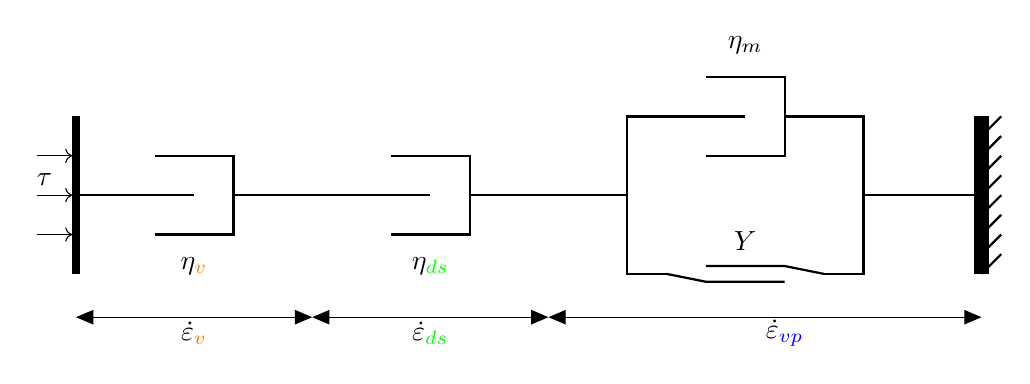
\begin{tikzpicture}
%\draw[fill=gray!23,gray!23](0,0) rectangle (7,5);
%\draw[step=0.5cm,gray,very thin] (0,0) grid (12,5); %background grid

\node[] at (0.1,2.7) {$\tau$};
\draw[line width=1mm] (0.5,1.5) -- (0.5,3.5) ;   
\draw [->] (0,2.5) -- (0.45,2.5);
\draw [->] (0,2) -- (0.45,2);
\draw [->] (0,3) -- (0.45,3);

\draw[thick] (0.5,2.5) -- (2,2.5) ;   
\draw[thick] (2.5,2.5) -- (5,2.5) ;   
\draw[thick] (5.5,2.5) -- (7.5,2.5) ;   
\draw[thick] (10.5,2.5) -- (12,2.5) ;   

% v damper
\draw[thick] (1.5,3) -- (2.5,3) -- (2.5,2) -- (1.5,2);  
% ds damper
\draw[thick] (4.5,3) -- (5.5,3) -- (5.5,2) -- (4.5,2);  
% m damper
\draw[thick] (8.5,4) -- (9.5,4) -- (9.5,3) -- (8.5,3);  

\node[] at (2,1.6) {$\eta_{\color{orange}v}$};
\node[] at (5,1.6) {$\eta_{\color{green}ds}$};
\node[] at (9,4.4) {$\eta_m$};

\draw[thick] (9,3.5) -- (7.5,3.5) -- (7.5,1.5) -- (8,1.5);  
\draw[thick] (9.5,3.5) -- (10.5,3.5) -- (10.5,1.5) -- (10,1.5);  

\draw[thick] (8,1.5) -- (8.5,1.4) -- (9.5,1.4) ;   
\draw[thick] (8.5,1.6) -- (9.5,1.6) -- (10,1.5) ;   

\node[] at (9,1.92) {$Y$};

%wall
\draw[line width=2mm] (12,1.5) -- (12,3.5) ;   
\draw[thick] (12,1.5) -- (12.25,1.75) ;   
\draw[thick] (12,1.75) -- (12.25,2) ;   
\draw[thick] (12,2) -- (12.25,2.25) ;   
\draw[thick] (12,2.25) -- (12.25,2.5) ;   
\draw[thick] (12,2.5) -- (12.25,2.75) ;   
\draw[thick] (12,2.75) -- (12.25,3) ;   
\draw[thick] (12,3) -- (12.25,3.25) ;   
\draw[thick] (12,3.25) -- (12.25,3.5) ;   

\draw[>=triangle 45, <->] (0.5,0.95) -- (3.5,0.95);
\draw[>=triangle 45, <->] (3.5,.95) -- (6.5,0.95);
\draw[>=triangle 45, <->] (6.5,0.95) -- (12,0.95);
\node[] at (2,0.75)   {$\dot\varepsilon_{\color{orange}v}$};
\node[] at (5,0.75)   {$\dot\varepsilon_{\color{green}ds}$};
\node[] at (9.5,0.75) {$\dot\varepsilon_{\color{blue}vp}$};

\end{tikzpicture}

\end{center}
The dislocation creep viscosity $\eta_{\color{green}ds}$ and effective 
viscoplastic viscosity $\eta_{\color{blue}vp}$ are given by 
\[
\eta_{\color{green}ds}(\dot\varepsilon) 
= \frac{1}{2} A^{-1/n} \dot{\varepsilon}^{-1+1/n} \exp \frac{Q}{nRT}
\qquad
\text{and}
\qquad
\eta_{\color{blue}vp}(\dot\varepsilon) 
= \frac{p \sin \phi + c \cos \phi}{2 \dot{\varepsilon}}  + \eta_{m}
\]
Note that these expressions are functions of $\dot\varepsilon$, the nature of which will be specified later. 
As documented in Section~\ref{MMM-ss:srpart}, 
the partitioning of the total strain rate into a viscous creep component and a viscoplastic component 
is not trivial.  
The algorithm then works as follows:

\begin{enumerate}
%%%%%%%%%%%%%%%%%
\item Assume we know $\dot\varepsilon_T$ (from previous iteration), 
as well as the yield value  $Y = p\; \sin\phi + c \; \cos \phi$ and $\eta_m$ (Here the 'T' stands 
for 'total').

%%%%%%%%%%%%%%%%%
\item We start by assuming that the plasticity element is not active 
($\dot{\varepsilon}_{\color{blue}vp}=0$, $\dot{\varepsilon}_{\color{green}ds}
+\dot{\varepsilon}_{\color{orange} v} =\dot{\varepsilon}_T$): 

We use the technique explained here after to compute the partitioning of the strain rate
and recover the stress $\tau$ and the dislocation creep effective viscosity
is given by 
\begin{eqnarray}
\eta_{\color{green}ds} &=& \frac{1}{2} A^{-1/n} 
\dot{\varepsilon}_{\color{green}ds}^{-1+1/n} \exp \left( \frac{Q}{nRT} \right) \nn\\
\eta_v &=& \frac{\tau}{2 \dot{\varepsilon}_{\color{orange}v}}  \nn
\end{eqnarray}
\begin{lstlisting}
eta_ds = 0.5*A**(-1./nnn)*np.exp(Q/nnn/Rgas/T)*eps_ds**(1./nnn-1.)
eps_v=tau/2/eta_v
\end{lstlisting}
The effective viscosity of both dampers is given by 
\[
\eta_{i\text eff}=\frac{1}{1/\eta_{\color{orange}v}+1/\eta_{\color{green}ds}}
\]
\begin{lstlisting}
etaeff=1./(1./eta_v+1./eta_ds)
\end{lstlisting}

%%%%%%%%%%%%%%%%%
\item if $\tau =2 {\eta}_{eff} \dot\varepsilon_T < Y$ the stress is below the yield stress value 
and the plasticity element is indeed not active. 
Simply return ${\eta}_{eff}$ in the material model.
\begin{lstlisting}
eps_vp=0
\end{lstlisting}

\item if $\tau=2 \eta_{eff} \dot\varepsilon_T > Y$ the stress is above the 
yield value, which is not allowed. In this case the plastic element must be present 
and active and the linear viscous and dislocation creep viscous dampers are then 
in series with the viscoplastic element. 
They  respectively deform with a strain rate $\dot{\varepsilon}_{\color{orange}v}$, 
$\dot{\varepsilon}_{\color{green}ds}$ and $\dot\varepsilon_{\color{blue}vp}$ 
(all under the same tress $\tau$) 
and we have  
$\dot\varepsilon_T = \dot{\varepsilon}_{\color{orange}v} +
\dot{\varepsilon}_{\color{green}ds} + \dot\varepsilon_{\color{blue}vp}$ so:

\begin{eqnarray}
\dot\varepsilon_T 
-\dot{\varepsilon}_{\color{orange}v} 
-\dot{\varepsilon}_{\color{green}ds}(\tau) 
&=& \dot\varepsilon_{\color{blue}vp}(\tau)  \nonumber\\
\dot\varepsilon_T 
-\dot{\varepsilon}_{\color{orange}v} 
-\dot{\varepsilon}_{\color{green}ds}(\tau) 
&=& \frac{\tau}{2 \eta_{\color{blue}vp}}  \nn\\
\dot\varepsilon_T 
-\dot{\varepsilon}_{\color{orange}v} 
-\dot{\varepsilon}_{\color{green}ds}(\tau) 
&=& \frac{\tau}{2 \left( \frac{Y}{2\dot\varepsilon_{\color{blue}vp}(\tau)} + \eta_m  \right)} 
\nonumber\\
\dot\varepsilon_T 
-\dot{\varepsilon}_{\color{orange}v} 
-\dot{\varepsilon}_{\color{green}ds}(\tau) 
&=&
\frac{\tau}{2 \left( \frac{Y}{2 (
\dot\varepsilon_T 
-\dot{\varepsilon}_{\color{orange}v}   
-\dot{\varepsilon}_{\color{green}ds}(\tau)  )} + \eta_m  \right)} \nonumber 
\\
2 [
\dot\varepsilon_T 
-\dot{\varepsilon}_{\color{orange}v}(\tau) 
-\dot{\varepsilon}_{\color{green}ds}(\tau)
]
\left( \frac{Y}{2 (
\dot\varepsilon_T 
-\dot{\varepsilon}_{\color{orange}v} 
-\dot{\varepsilon}_{\color{green}ds}(\tau) )} + \eta_m  \right) &=& \tau 
\nonumber\\
Y + 2 (
\dot\varepsilon_T 
-\dot{\varepsilon}_{\color{orange}v}(\tau)  
-\dot{\varepsilon}_{\color{green}ds}(\tau) ) \eta_m  &=& \tau \nonumber 
\end{eqnarray}
We must then find the zero of the function ${\cal F}(\tau)$: 
\begin{eqnarray}
{\cal F}(\tau) 
&=& Y + 2 [
\dot\varepsilon_T 
-\dot{\varepsilon}_{\color{orange}v}(\tau)   
-\dot{\varepsilon}_{\color{green}ds}(\tau) 
]\eta_m -\tau \nonumber\\
&=& Y + 2 \left[ 
\dot\varepsilon_T -\frac{\tau}{2\eta_v} -A \tau^n \exp \left(-\frac{Q}{RT}\right) 
\right]\eta_m -\tau \nn
\end{eqnarray}
Because dislocation creep involves the $n$-th power of the stress (and $n$ need not be an integer!) 
finding the value of the stress for which ${\cal F}=0$ is not straightforward.
This equation can be solved with a Newton-Raphson algorithm
and the iterations will be of the form:
\[
\tau_{n+1} = \tau_n - \frac{{\cal F}(\tau_n)}{{\cal F}'(\tau_n)}
\]
where the derivative of the function ${\cal F}$ with respect to $\tau$ reads:
\begin{eqnarray}
\frac{\partial {\cal F}}{\partial \tau} 
= -\frac{\eta_m}{\eta_v}-2 \eta_m n A \tau^{n-1} \exp \left(-\frac{Q}{RT}\right) -1 
\end{eqnarray}
Iterations require a starting value for $\tau$: we logically use the one obtained just 
above. Iterations stop when ${\cal F}<10^{-6}$.  
A maximum of 30 iterations is allowed.

\begin{lstlisting}
while abs(func)>1e-6:
   eps_ds=A*tau**nnn*np.exp(-Q/Rgas/T)
   eps_v=tau/2/eta_v
   func=Y + 2*(E2-eps_ds-eps_v)*eta_m - tau
   funcp=-eta_m/eta_v -2*eta_m*nnn*A*tau**(nnn-1)*np.exp(-Q/Rgas/T)-1
   tau-=func/funcp
   it+=1
   if it>30:
      break
#end while
\end{lstlisting}

\item Once $\tau$ has been found, one can compute 
\begin{eqnarray}
\dot{\varepsilon}_{\color{green}ds}(\tau)&=&A \tau^n \exp \left(-\frac{Q}{RT}\right)
\qquad 
\Rightarrow 
\qquad 
\eta_{\color{green}ds}(\dot\varepsilon_{\color{green}ds}) 
= \frac{1}{2} A^{-1/n} \dot{\varepsilon}_{\color{green}ds}^{-1+1/n} \exp \frac{Q}{nRT} \nn\\
\dot{\varepsilon}_{\color{orange}v}(\tau)&=&\frac{\tau}{2\eta_v}  \nn
\end{eqnarray}
\begin{lstlisting}
eps_ds=A*tau**nnn*np.exp(-Q/Rgas/T)
eta_ds = 0.5*A**(-1./nnn)*np.exp(Q/nnn/Rgas/T)*eps_ds**(1./nnn-1.)
eps_v=tau/2/eta_v
\end{lstlisting}
then 
$\dot{\varepsilon}_{\color{blue}vp}
=\dot{\varepsilon}_T 
-\dot{\varepsilon}_{\color{orange}v}(\tau) 
-\dot{\varepsilon}_{\color{green}ds}(\tau)$,
and then 
\[
\eta_{\color{blue} vp}(\dot\varepsilon_{\color{blue} vp}) 
= \frac{p \sin \phi + c \cos \phi}{2 \dot{\varepsilon}_{\color{blue}vp}}  + \eta_{m}
\]
\item 
Ultimately the effective viscosity at every quadrature point is computed as follows:
\[
\eta_{eff} = \left(
\frac{1}{\eta_{\color{orange}v}} + 
\frac{1}{\eta_{\color{green}ds}}  + 
\frac{1}{\eta_{\color{blue}vp}}  
\right)^{-1}
\]
\begin{lstlisting}
etaeff=1/(1/eta_v+1/eta_ds+1/eta_vp)
\end{lstlisting}

\end{enumerate}

%I set $\dot{\varepsilon}=10^{-15}\si{\per\second}$ in the viscosity function, 
%just so that the rheological model does not explode.
 
By construction, the viscosity is also maintained between $\eta_{m}\ge \SI{1e19}{\pascal}$ 
and $\eta_{v}=\SI{1e25}{\pascal}$. 

\begin{center}
\includegraphics[width=11cm]{python_codes/fieldstone_70/images/fig2}\\
{\captionfont Figure taken from \cite{dudy20}}
\end{center}

\begin{center}
\includegraphics[width=9cm]{python_codes/fieldstone_70/images/aspect_sr}\\
\includegraphics[width=9cm]{python_codes/fieldstone_70/images/aspect_eta}\\
{\captionfont Obtained with \aspect (see cookbook)}
\end{center}


%\newpage
%......................
%\paragraph{Extension}. 

%\begin{center}
%\includegraphics[width=7cm]{python_codes/fieldstone_70/extension/u}
%\includegraphics[width=7cm]{python_codes/fieldstone_70/extension/v}\\
%\includegraphics[width=7cm]{python_codes/fieldstone_70/extension/vel}
%\includegraphics[width=7cm]{python_codes/fieldstone_70/extension/q}\\
%\includegraphics[width=7cm]{python_codes/fieldstone_70/extension/e}
%\includegraphics[width=7cm]{python_codes/fieldstone_70/extension/etaeff}\\
%\includegraphics[width=6cm]{python_codes/fieldstone_70/extension/conv.pdf}
%\includegraphics[width=6cm]{python_codes/fieldstone_70/extension/pressure.pdf}\\
%\includegraphics[width=6cm]{python_codes/fieldstone_70/extension/tau.pdf}\\
%extension, resolution 150x45, 100 nl iterations only.
%\end{center}

%\newpage
%......................
%\paragraph{Compression}. 

%\begin{center}
%\includegraphics[width=7cm]{python_codes/fieldstone_70/compression/u}
%\includegraphics[width=7cm]{python_codes/fieldstone_70/compression/v}\\
%\includegraphics[width=7cm]{python_codes/fieldstone_70/compression/vel}
%\includegraphics[width=7cm]{python_codes/fieldstone_70/compression/q}\\
%\includegraphics[width=7cm]{python_codes/fieldstone_70/compression/e}
%\includegraphics[width=7cm]{python_codes/fieldstone_70/compression/etaeff}\\
%\includegraphics[width=6cm]{python_codes/fieldstone_70/compression/conv.pdf}
%\includegraphics[width=6cm]{python_codes/fieldstone_70/compression/pressure.pdf}\\
%\includegraphics[width=6cm]{python_codes/fieldstone_70/compression/tau.pdf}\\
%extension, resolution 150x45, 100 nl iterations only.
%\end{center}

 %%%%%%%%%%%%%%%%%%%%%%%%%%%%%%%%%%%%%%%%%%%%%%%%%%%%%%%%%%%%%%%%%%%%%%

\chapter{S40RTS in an annulus \label{f71}} %%%%%%%%%%%%%%%%%%%%%%%%%%%%%%%%%%%%%%%%%%%%%%%%%%%%%%%%%%%%%%%%%%% 71
\includegraphics[height=1.5cm]{images/pictograms/visualisation}
\includegraphics[height=1.5cm]{images/pictograms/tools}

\lstinputlisting[language=bash,basicstyle=\small]{python_codes/fieldstone_71/keywords.ascii}

\begin{center}
Code at \url{https://github.com/cedrict/fieldstone/tree/master/python_codes/fieldstone_71}
\end{center}

\par\noindent\rule{\textwidth}{0.4pt}

{\sl This stone was developed in collaboration with Rens Elbertsen}. \index{contributors}{R. Elbertsen}

\par\noindent\rule{\textwidth}{0.4pt}
%%%%%%%%%%%%%%%%%%%%%%%%%%%%%%%%%%%%%%%%%%%%%%%%%%%%%%%%%%%%%%%%%%%%%%%%%%%%%%%%%%%%%%%%%%%%%%

I neeed:
- free slip bc
- max res ?
- crust/lith
- rotated plane 
- compare with submachine


%_____________________________________________________________________________
\subsubsection*{Radial viscosity profiles}

\

In this section we describe the different density profiles used to in the convection model. We assume that viscosity is purely a function of depth. The user can choose a viscosity profile by changing the parameter \texttt{case}.

Five radial viscosity profiles are available:
\begin{itemize}
\item The first viscosity profile is a constant viscosity for all depths of $10^{22}$ Pa s. 
This value is an estimated value of what is normally found in the literature. This is \texttt{visc\_case = 0}. 

\item The second viscosity profile comes from Yoshida et al (2001) \cite{yohk01}. It uses three different regions: lithosphere (0 km to 150 km), upper mantle (150 km to 670 km) and lower mantle (670 km to 2900 km). The function uses an if-statement to return the right value for the given depth. This is \texttt{case = 1}.

\item The third viscosity profile comes from Steinberger \& Holmes (2008) \cite{stho08} 
which is comparable to \cite{stca06}, but of the latter no available data was available. 
Data is read from the file \texttt{visc\_STHO08.dat}. 
This is \texttt{case = 2}.

\item The fourth and fifth profile come from Ciskova et al (2012) \cite{civs12}. 
Data is read from the file \texttt{visc\_CIVS12.dat}. 
The paper showcases two main families of radial viscosity profiles in literature. Family A, which has a sharp 
increase below the 660 km transition zone and remains constant for most of the lower mantle 
and family B which is much smoother over the transition zone and increases with depth in the lower mantle. 
Family A can be chosen by \texttt{case = 3} and family B can be chosen by \texttt{case = 4}.

\end{itemize}

\begin{center}
\includegraphics[width=10cm]{python_codes/fieldstone_71/images/visc}
\end{center}


%_____________________________________________________________________________
\subsubsection*{Cross section of the Earth}

Several parameters are implemented which can be modified to get any cross section of the Earth. 

The parameter \texttt{lon\_start} specifies at which longitude we start reading data from the S40RTS model. The model always starts filling the annulus on the right ($x=1, y=0$ on the unit circle) continuing in the counter-clockwise direction with increasing longitudes. If we set the parameter \texttt{plane\_angle} (explained in the next subsection) to 0 we have an equatorial cross section through the Earth that starts at the longitude \texttt{lon\_start}.

The parameter \texttt{plane\_angle} indicates the angle the plane of the cross section is making with the equatorial plane. The longitude specified by \texttt{lon\_start} always is at latitude 0. Latitudes will be increased as a result of the \texttt{plane\_angle} on the northern hemisphere and decreased on the southern hemisphere. Setting the \texttt{plane\_angle} to 90 gives us a cross section through both poles and the longitude specified by \texttt{lon\_start}.



%_____________________________________________________________________________
\subsubsection*{Loading of the Spherical Harmonics, computing $\delta \ln V_s$}

In this stone we wish to use the shear wave velocity model S40RTS \cite{ridv11} 
as the main source of information 
to build a temperature anomaly/density anomaly model of the mantle. 

Variations of the shear wave velocity are stored in the form of spherical harmonics coefficients. 
We make use of an already existing code written by Ross Ronan Maguire
(available at \url{https://github.com/romaguir/sph_models}
to read the values of $d \ln{V_S}$ for a section of the Earth. 
The code is modified such that we read in $d \ln{V_S}$ for every nodal point in the annulus domain. 
Note that the returned value had to be scaled down by a factor of $\sqrt{2}$ to obtain identical figures to 
those of the original paper or those obtained with SubMachine\footnote{\url{https://www.earth.ox.ac.uk/~smachine/cgi/index.php}}.  




There are three different functions in the original code that enables us to read 
the spherical harmonics data: \texttt{read\_splines}, \texttt{read\_sph} 
and \texttt{find\_spl\_vals}. The function \texttt{read\_sph} reads the data from the spherical 
harmonics data file. Thereafter, we loop over all the nodal points. The loop starts at the 
deepest circle of nodes and loops counter-clockwise over this circle before continuing with the 
next circle that is one row of nodal points outwards. The function \texttt{find\_spl\_vals} 
reads the values for a specific depth, meaning that we only have to read these once when we 
start a new circle of nodal points. This function makes use of the other function \texttt{read\_splines}. 
Once we have the correct splines we loop over all nodal points at this depth and calculate the 
value of $\delta \ln{V_s}$ for all these points. The value of $\delta \ln{V_s}$ 
is stored in the array \texttt{d\_ln\_vs}.

\begin{center}
\includegraphics[width=7cm]{python_codes/fieldstone_71/images/sub_cross_section_01}
\includegraphics[width=7cm]{python_codes/fieldstone_71/images/sub_cross_section_02}\\
{\captionfont Taken from SubMachine\footnote{\url{https://www.earth.ox.ac.uk/~smachine/cgi/index.php}}.
Cross sections of the mantle for S20RTS and S40RTS models. 
Left: latitude=0, longitude between 0 and 179.
Right: latitude=0, longitude between -179 and 0.}
\end{center}

\begin{center}
\includegraphics[width=9cm]{python_codes/fieldstone_71/images/dlnvsS40RTS_equator}\\
{\captionfont S40RTS, nelr=50}
\end{center}


%_____________________________________________________________________________
\subsubsection*{Converting $\delta \ln V_s$ to $\delta \rho$}

We assume that there is a direct scaling from the shear wave velocity anomaly to the density anomaly, i.e. 
we assume that all anomalies in $\delta \ln{V_s}$ are the result of temperature perturbations and 
not of differences in composition. 
We use the following formula to obtain the $\delta \ln{\rho} $ values:
\[
\delta \ln{\rho(r, \theta, \phi)} = \xi(r) \cdot \delta \ln{V_s(r, \theta, \phi)} 
\]
where $\xi$ is the scaling factor that is depth dependent. We will go into more depth for this factor in the following subsections. To get the values for $\delta \rho(r, \theta, \phi)$ we use the following formula:
\[
\delta \ln{\rho(r, \theta, \phi)} = \frac{\delta \rho(r, \theta,\phi)}{\rho_\text{ref}} 
\]
where $\rho_\text{ref}$ is the reference density, which in our case for the S40RTS model is the PREM model 
\cite{dzan81}. In the following section we will show which scalings are implemented in the model and how 
they are implemented. The user can choose a scaling by changing the parameter \texttt{xi\_case}. 
The value for $\xi$ is stored in the array \texttt{xi\_nodal}, 
the value for $\rho_\text{PREM}$ is stored in the array \texttt{rho\_prem\_nodal}, 
the value for $\delta \ln{\rho}$ is stored in the array \texttt{d\_ln\_rho\_nodal} 
and the value of $\delta \rho$ is stored in the array \texttt{d\_rho\_nodal}.

There are three options in the code to compute the $\xi$ coefficient:
\begin{itemize}
\item Constant $\xi$. The first scaling that is used is a constant value for $\xi$ of 0.25. 
This is \texttt{xi\_case = 0}. The factor 0.25 is an estimated average of what is normally found in 
literature. An overview of the three different cases can be found hereunder:

\begin{center}
\includegraphics[width=8cm]{python_codes/fieldstone_71/images/xi}
\end{center}

\item The second scaling that is used comes from Steinberger \& Calderwood (2006) \cite{stca06}. 
Data is read from the file \texttt{data/xi/xi\_stca06.ascii}. 

\item The third scaling that is used comes from Moulik \& Ekstrom (2016) \cite{moek16}. 
Data is read from the file \texttt{data/xi/xi\_moek16.ascii}. 
A very noticeable difference between this scaling and the scaling of \cite{stca06} 
is that for the upper mantle the value for $\xi$ is slightly higher and for the lowermost lower mantle 
the value for $\xi$ is negative.
\end{itemize}




 %%%%%%%%%%%%%%%%%%%%%%%%%%%%%%%%%%%%%%%%%%%%%%%%%%%%%%%%%%%%%%%%%%%%%%

\chapter{quadrilateral MINI - the $Q_1^+\times Q_1$ element \label{f72}} %%%%%%%%%%%%%%%%%%%%%%%%%%%%%%%%%%%%% 72
%\lstinputlisting[language=bash,basicstyle=\small]{python_codes/fieldstone_72/keywords.ascii}

\begin{center}
Code at \url{https://github.com/cedrict/fieldstone/tree/master/python_codes/fieldstone_72}
\end{center}

\par\noindent\rule{\textwidth}{0.4pt}

%%%%%%%%%%%%%%%%%%%%%%%%%%%%%%%%%%%%%%%%%%%%%%%%%%%%%%%%%%%%%%%%%%%%%%%%%%%%%%%%%%%%%%%%%%%%%%%%%%%%

\index{stopics}{$Q_1^+\times Q_1$}


%--------------------------------------
\section*{Manufactured solution \#1}

The analytical solution originates in \textcite{lami17} (2017).
The velocity and pressure are given by
\begin{eqnarray}
u(x,y)&=&-2x^2y(2y-1)(x-1)^2(y-1) \\
v(x,y)&=& 2xy^2(2x-1)(x-1)(y-1)^2 \\
p(x,y)&=& x(1-x)(1-2y)
\end{eqnarray}
Boundary conditions are no-slip on all sides of the unit square. 
The corresponding body force terms are derived in Section~\ref{MMM-ss:mms11}. 


The quadrilateral MINI element used here also originates in the same article 
and comes in two flavours with two different bubble functions $b_1$ and $b_2$
as explained in Section~\ref{MMM-ss:quadmini}.
The two bubble functions are (in reduced coordinates $-1 \leq r,s \leq 1$):
\begin{eqnarray}
b_1(r,s) &=& (1-r^2)(1-s^2)\cdot (1-r)(1-s)\\
b_2(r,s) &=& (1-r^2)(1-s^2)\cdot (1+\beta(r+s))
\end{eqnarray}
The common term to both bubbles insures that the bubble is exactly zero on all four edges of the 
element. What differentiates them is the remaining term, which is bilinear ($b_1$) or linear ($b_2$). 
Both also satisfy $b_1(0,0)=b_2(0,0)=1$. The paper uses $\beta=1/4$.

The velocity and pressure fields for the benchmark are shown hereunder:
\begin{center}
\includegraphics[width=7cm]{python_codes/fieldstone_72/results/mms/vel}
\includegraphics[width=7cm]{python_codes/fieldstone_72/results/mms/p}
\end{center}

During the debugging process I ended up 
implementing various Gauss quadratures schemes, from $2^2$ to $6^2$ points but the results
show that $2^2$ quadrature points per element are sufficient since the more expensive quadratures
yield identical results. 
The results from the article are somewhat different than mine but I suspect that what the 
author measured could be different than what I measure (see Table 1,2 in \cite{lami17}). 
The trends are similar though, with $b_2$ performing better than $b_1$:

\begin{center}
\includegraphics[width=8cm]{python_codes/fieldstone_72/results/mms/errors_v}
\includegraphics[width=8cm]{python_codes/fieldstone_72/results/mms/errors_p}\\
{\captionfont Left: velocity error in $L_2$ norm; Right: pressure error in $L_2$ norm.
Resolutions from $8\times8$ until $80\times80$.}
\end{center}

The root mean square velocity is also measured for both bubble functions.
As above we see that $b_2$ performs better than $b_1$:
\begin{center}
\includegraphics[width=9cm]{python_codes/fieldstone_72/results/mms/vrms}
\end{center}


%................................................
\subsubsection{Influence of mesh nodes position:} 
I have also repeated these 
experiments with a mesh whose internal nodes have been 
randomly moved by up to $\pm$20\% of $h_x$ or $h_y$ around the initial position. 

\begin{center}
\includegraphics[width=5.7cm]{python_codes/fieldstone_72/results/mms/area16}
\includegraphics[width=5.7cm]{python_codes/fieldstone_72/results/mms/area32}
\includegraphics[width=5.7cm]{python_codes/fieldstone_72/results/mms/area64}\\
{\captionfont area of elements for randomized meshes. Left to right: 16x16, 32x32, 64x64}
\end{center}


\begin{center}
\includegraphics[width=5.7cm]{python_codes/fieldstone_72/results/mms/errors_v_rand}
\includegraphics[width=5.7cm]{python_codes/fieldstone_72/results/mms/errors_p_rand}
\includegraphics[width=5.7cm]{python_codes/fieldstone_72/results/mms/vrms_rand}
\end{center}

We find that the error convergence rate is unchanged for velocities but is now less 
for pressure (higher than 1, lower than 1.5). 

%..............................
\subsubsection{Another bubble?} 
To make the point that the bubble function must contain the (bi-)linear term, 
I have created a third bubble function which is simply $b_3(r,s)=(1-r^2)(1-s^2)$.
Technically it is zero on the sides and 1 in the middle so it fulfills the 
same requirements as the other 2 bubble functions. 
However, we see that this function is not sufficient to stabilise the element as the pressure 
showcases a typical error mode:
\begin{center}
\includegraphics[width=6cm]{python_codes/fieldstone_72/results/mms/p_b3}
\includegraphics[width=6cm]{python_codes/fieldstone_72/results/mms/p_error_b3}\\
{\captionfont Left: pressure field as obtained with $b_3$; right: pressure error.}
\end{center}


%..............................
\subsubsection{influence of $\beta$:} Finally, 
I use a $2\times 2$ quadrature and look at 
the errors and the vrms for various values of $\beta$:
\begin{center}
\includegraphics[width=5cm]{python_codes/fieldstone_72/results/mms/errors_v_beta}
\includegraphics[width=5cm]{python_codes/fieldstone_72/results/mms/errors_p_beta}
\includegraphics[width=5cm]{python_codes/fieldstone_72/results/mms/vrms_beta}
\end{center}
It looks like $\beta\in[0.0001,0.01]$ does better than all other higher values. 
Also, looking at the 
field in Paraview, no trace of the error modes as we just saw above.
The difference between 0.01 and 0.25 is somewhat small, but values of $\beta$ above 0.5 
clearly yield less accurate results. 

I can also plot these same results in a different way, i.e. placing $\beta$ on the horizontal axis:

\begin{center}
\includegraphics[width=5cm]{python_codes/fieldstone_72/results/mms/errors_v_beta2}
\includegraphics[width=5cm]{python_codes/fieldstone_72/results/mms/errors_p_beta2}
\includegraphics[width=5cm]{python_codes/fieldstone_72/results/mms/vrms_beta2}\\
{\captionfont From left to right: velocity error, pressure error and vrms as a function 
of the parameter $\beta$, for 5 different resolutions. The dotted line corresponds to $\beta=1/4$ as used in \cite{lami17}.}
\end{center}

One could conclude that $\beta=10^{-4}-10^{-2}$ 
would be a better choice but the question remains whether these
conclusions hold for other benchmarks. We will see later 
that $\beta=1/4$ is actually preferable to these very low values.


\subsubsection{Looking at the condition number of the $\K$ matrix} 
(remember: $\K$ is the 1,1 block of the
Stokes matrix). 
I have computed the condition number of the $\K$ matrix for both bubbles and for various mesh resolutions. 
We see that the bubble 1 yields condition numbers substantially higher than bubble 2, both increasing 
quadratically with $h$. This is rather critical is (for instance) a conjugate gradient solver is used 
is used on this matrix.

\begin{center}
\includegraphics[width=6cm]{python_codes/fieldstone_72/results/mms/eigenvalues/e}
\end{center}

%_____________________________________
\section*{Manufactured solution \#2}

This is the second manufactured solution 
mentioned in Lamichhane \cite{lami17}. It is presented in Section~\ref{MMM-ss:mms2}.
It is for a unit square with $\eta=1$ and the smooth exact solution is
\begin{eqnarray}
u(x,y) &=& x+x^2 - 2xy+x^3 - 3xy^2 + x^2y \\
v(x,y) &=& -y-2xy+y^2 -3x^2y + y^3 - xy^2 \\
p(x,y) &=& xy+x+y+x^3y^2 - 4/3
\end{eqnarray}
Note that the pressure obeys $\int_{\Omega} p \; d\Omega = 0$. The analytical 
velocity is prescribed on the boundary of the domain. 
The corresponding body force is:
\begin{eqnarray}
b_x &=& 3x^2y^2 -y-1   \\
b_y &=& 2x^3y+3x-1 
\end{eqnarray}


\begin{center}
\includegraphics[width=7cm]{python_codes/fieldstone_72/results/mms2/errors_v}
\includegraphics[width=7cm]{python_codes/fieldstone_72/results/mms2/errors_p}\\
{\captionfont Velocity and pressure error convergence as a function of the mesh size $h$ for
meshes $8\times 8$ up to $128\times 128$.}
\end{center}


The root mean square velocity is also measured for both bubble functions.
As above we see that $b_2$ performs better than $b_1$:
\begin{center}
\includegraphics[width=9cm]{python_codes/fieldstone_72/results/mms2/vrms}
\end{center}


\begin{center}
\includegraphics[width=5cm]{python_codes/fieldstone_72/results/mms2/u}
\includegraphics[width=5cm]{python_codes/fieldstone_72/results/mms2/v}
\includegraphics[width=5cm]{python_codes/fieldstone_72/results/mms2/vel}\\
{\captionfont Velocity field as obtained on $32\times 32$ grid. Left: $x-$component,
middle: $y-$component, right: velocity vector magnitude.}
\end{center}

\begin{center}
\includegraphics[width=7cm]{python_codes/fieldstone_72/results/mms2/error_v1}
\includegraphics[width=7cm]{python_codes/fieldstone_72/results/mms2/error_v2}\\
{\captionfont Velocity error for bubble function 1 (left) and bubble function 2 (right). 
$b_2$ maximum error is about half of $b_1$ error.}
\end{center}

\begin{center}
\includegraphics[width=7cm]{python_codes/fieldstone_72/results/mms2/p1}
\includegraphics[width=7cm]{python_codes/fieldstone_72/results/mms2/p2}\\
{\captionfont Pressure field obtained with bubble function 1 (left) and bubble function 2 (right).
Scale has been voluntarily set to analytical values scale for both.}
\end{center}

\begin{center}
\includegraphics[width=7cm]{python_codes/fieldstone_72/results/mms2/error_p1}
\includegraphics[width=7cm]{python_codes/fieldstone_72/results/mms2/error_p2}\\
{\captionfont Pressure error field obtained with bubble function 1 (left) and bubble function 2 (right). Notice the 
different error magnitudes between both!}
\end{center}

The conclusions are identical to those obtained with the first manufactured solution. 
The second bubble function (here with $\beta=1/4$) performs better. While velocity error
convergence rates are quadratic for both bubbles, the pressure error is substantially lower
for bubble 2 (although its rate is slightly lower than bubble 1 -- both are still 
superconvergent). This is illustrated above where we see that the pressure field obtained 
with bubble 1 showcases strong ripples in the upper right corner.     



%_____________________________________
\section*{The SolCx benchmark}

Because of the viscosity jump at $x=L_x/2$, it has been widely reported that 
error convergence rates depend on wheter the number of element in the $x-$direction 
is even or odd.

\begin{center}
\includegraphics[width=5cm]{python_codes/fieldstone_72/results/solcx/errors_v_even}
\includegraphics[width=5cm]{python_codes/fieldstone_72/results/solcx/errors_p_even}
\includegraphics[width=5cm]{python_codes/fieldstone_72/results/solcx/vrms_even}\\
\includegraphics[width=5cm]{python_codes/fieldstone_72/results/solcx/errors_v_odd}
\includegraphics[width=5cm]{python_codes/fieldstone_72/results/solcx/errors_p_odd}
\includegraphics[width=5cm]{python_codes/fieldstone_72/results/solcx/vrms_odd}
\end{center}

Velocity error convergence rates are 2 for even numbers of elements and 1 for odd numbers, 
such as for the Q1Q1 stab. 
Pressure error convergence rate seems to be 0.5 for odd numbers of elements and
0.65 for even numbers ... 

\begin{center}
\includegraphics[width=5cm]{python_codes/fieldstone_72/results/solcx/vel}
\includegraphics[width=5cm]{python_codes/fieldstone_72/results/solcx/p}
\includegraphics[width=5cm]{python_codes/fieldstone_72/results/solcx/p_error}
\end{center}

We see that the pressure showcases an strong error (even at high resolution)
along the interface. 


%_____________________________________
\section*{The SolKz benchmark}

\begin{center}
\includegraphics[width=5cm]{python_codes/fieldstone_72/results/solkz/errors_v}
\includegraphics[width=5cm]{python_codes/fieldstone_72/results/solkz/errors_p}
\includegraphics[width=5cm]{python_codes/fieldstone_72/results/solkz/vrms}
\end{center}

We find that velocity and pressure errors converge quadratically, with 
once again $b_2$ better than $b_1$.


%_____________________________________
\section*{The SolVi benchmark}


\begin{center}
\includegraphics[width=7cm]{python_codes/fieldstone_72/results/solvi/vel}
\includegraphics[width=7cm]{python_codes/fieldstone_72/results/solvi/p}\\
{\captionfont Resolution $128\times128$ - bubble 1 }
\end{center}


\begin{center}
\includegraphics[width=5cm]{python_codes/fieldstone_72/results/solvi/errors_v}
\includegraphics[width=5cm]{python_codes/fieldstone_72/results/solvi/errors_p}
\includegraphics[width=5cm]{python_codes/fieldstone_72/results/solvi/vrms}
\end{center}



%_____________________________________
\section*{The Stokes Sphere}

This experiment is the benchmark of Section~\ref{MMM-ss:stokes_sphere2D}. 
The density is assigned directly to the 
quadrature point by means of a function. Inside the disc of radius 0.123456789 centered in the domain 
the density is set to 1.01 while it is set to 1 outside 
(viscosities are respectively 1000 and 1). The gravity is $|g_y|=1$ and 
free-slip boundary conditions are implemented on all sides. 

On the following figures the min/max of the pressure in the domain and the vrms 
are shown for both bubble functions. We see that at low resolution the reported 
values show some variations but with increasing resolution the quantities converge to a single value:

\begin{center}
\includegraphics[width=7cm]{python_codes/fieldstone_72/results/sphere/pstats}
\includegraphics[width=7cm]{python_codes/fieldstone_72/results/sphere/vrms}
\end{center}

\begin{center}
\includegraphics[width=7cm]{python_codes/fieldstone_72/results/sphere/vel_b1}
\includegraphics[width=7cm]{python_codes/fieldstone_72/results/sphere/vel_b2}\\
\includegraphics[width=7cm]{python_codes/fieldstone_72/results/sphere/p_b1}
\includegraphics[width=7cm]{python_codes/fieldstone_72/results/sphere/p_b2}\\
{\captionfont Left is b1, Right is b2.}
\end{center}

It looks like $b_2$ yields more anomalous pressure modes inside the sphere, 
which is corroborated by the following figures which show the pressure 
at $x=L_x/2$ in both cases. However we also see that at high resolution both 
bubbles yield nearly identical pressure profiles and that the ripples have vanished. 

\begin{center}
\includegraphics[width=5cm]{python_codes/fieldstone_72/results/sphere/pline_b1_closed}
\includegraphics[width=5cm]{python_codes/fieldstone_72/results/sphere/pline_b2_closed}
\includegraphics[width=5cm]{python_codes/fieldstone_72/results/sphere/pline_b12_closed}\\
{\captionfont pressure profile for b1 (left) and b2 (middle) for different resolutions.}
\end{center}

One can also prescribe an open boundary condition at the top:

\begin{center}
\includegraphics[width=7cm]{python_codes/fieldstone_72/results/sphere/open/vel}
\includegraphics[width=7cm]{python_codes/fieldstone_72/results/sphere/open/p}
\end{center}


\begin{center}
\includegraphics[width=5cm]{python_codes/fieldstone_72/results/sphere/pline_b1_open}
\includegraphics[width=5cm]{python_codes/fieldstone_72/results/sphere/pline_b2_open}
\includegraphics[width=5cm]{python_codes/fieldstone_72/results/sphere/pline_b12_open}\\
{\captionfont pressure profile for b1 (left) and b2 (middle) for different resolutions.}
\end{center}





%_____________________________________
\section*{Rayleigh-Taylor instability}

This benchmark is carried out in Appendix D of Thieulot (2011) \cite{thie11}.
It consists of a two-layer system driven by gravity.
The mesh is modified so as to align with the sinusoidal perturbation.
Resolution and $\eta_2$ are varied on the following figures:

\begin{center}
\includegraphics[width=7cm]{python_codes/fieldstone_72/results/RT/area}
\includegraphics[width=7cm]{python_codes/fieldstone_72/results/RT/eta}\\
\includegraphics[width=7cm]{python_codes/fieldstone_72/results/RT/rho}
\includegraphics[width=7cm]{python_codes/fieldstone_72/results/RT/vel}
\end{center}


\begin{center}
\includegraphics[width=7cm]{python_codes/fieldstone_72/results/RT/vy_b1}
\includegraphics[width=7cm]{python_codes/fieldstone_72/results/RT/vy_b2}
\end{center}

Bubble 2 does better than bubble 1. Also, $\beta$ does not seem to play a role.

%_____________________________________
\section*{Sinking block}
This is the very same experiment as in Stone 53. It consists of a negatively buoyant 
square object falling in a fluid in a square domain. 
This particular experiment proved to be the 'downfall' of the $Q_1\times Q_1-stab$ element
since the stabilisation term is akin to a pressure diffusion and therefore
acts on the lithostatic pressure and also tends to smooth the effect of small 
density variations (Thieulot \& Bangerth, in prep.). 

Unless specified otherwise bubble 2 has $\beta=0.25$ by default.

%............................
\subsection*{Full density} 
Results indicate that the element performs adequately, especially the 
pressure field which looks smooth.  

\begin{center}
\includegraphics[width=7cm]{python_codes/fieldstone_72/results/block/full/density}
\includegraphics[width=7cm]{python_codes/fieldstone_72/results/block/full/viscosity}\\
\includegraphics[width=7cm]{python_codes/fieldstone_72/results/block/full/vel}
\includegraphics[width=7cm]{python_codes/fieldstone_72/results/block/full/p}\\
{\captionfont $64\times 64$. Viscosity ratio is 10, $\delta \rho=8$, bubble 1.}
\end{center}

We see that the element is capable of reprensenting a linear pressure profile
(the overpressure signal due to the block is negligible compared to the 
hydrostatic pressure).

\begin{center}
\includegraphics[width=10cm]{python_codes/fieldstone_72/results/block/full/plines}\\
{\captionfont Pressure profile measured at $x=L_x/2$ for various resolutions. Same parameters
as previous figure.}
\end{center}

As before we produce the characteristic figures of the velocity and pressure in the middle of the 
block as a function of the viscosity ratio and the density difference. The results obtained 
with the quadrilateral MINI element agree nicely with those obtained with the $Q_2\times Q_1$ element:
 
\begin{center}
\includegraphics[width=7cm]{python_codes/fieldstone_72/results/block/full/results_v}
\includegraphics[width=7cm]{python_codes/fieldstone_72/results/block/full/results_p}
\end{center}


\underline{Influence of $\beta$ parameter for bubble 2:} I set $\delta\rho=8$, resolution 64x64, $\eta^\star=10$,
and record the pressure profile 

\begin{center}
\includegraphics[width=10cm]{python_codes/fieldstone_72/results/block/full/betastudy/plines}
\end{center}

We can conclude that the bubble type and the value of $\beta$ do not seem to significantly affect 
the pressure profile in this case.

%............................
\subsection*{Reduced density} 
This is the same experiment as above but $\rho_1$ has been removed from the density
everywhere in the domain, so that the surrounding material has zero density 
and the block has a density $\delta \rho$.
The velocity and pressure field are then:

\begin{center}
\includegraphics[width=7cm]{python_codes/fieldstone_72/results/block/reduced/vel}
\includegraphics[width=7cm]{python_codes/fieldstone_72/results/block/reduced/p}\\
{\captionfont $64\times 64$. Viscosity ratio is 10, $\delta \rho=8$. bubble 1}
\end{center}

We then turn to the pressure along the vertical line $x=L_x/2$ as obtained with 
both bubble functions and find that both yield visually similar profiles:

\begin{center}
\includegraphics[width=7cm]{python_codes/fieldstone_72/results/block/reduced/plines_b1}
\includegraphics[width=7cm]{python_codes/fieldstone_72/results/block/reduced/plines_b2}\\
{\captionfont Pressure profile measured at $x=L_x/2$ for various resolutions and for both bubble functions.
Left is bubble 1, right is bubble 2.}
\end{center}

I hereafter plot the pressure profiles for both bubble functions at the highest resolution, i.e. $96\times 96$.
We see that differences are somewhat minimal, although bubble 2 yields a pressure above the block which 
showcases worrying oscillations. Also the results are remarquably similar to those obtained with the Taylor-Hood
$Q_2\times Q_1$ element:

\begin{center}
\includegraphics[width=7cm]{python_codes/fieldstone_72/results/block/reduced/plines_b12}
\includegraphics[width=7cm]{python_codes/fieldstone_72/results/block/reduced/plines_b12_zoom}
\end{center}

Finally the velocity and pressure inside the block unsurprisingly match nicely with those obtained with the Taylor-Hood
$Q_2\times Q_1$ element:

\begin{center}
\includegraphics[width=7cm]{python_codes/fieldstone_72/results/block/reduced/results_v}
\includegraphics[width=7cm]{python_codes/fieldstone_72/results/block/reduced/results_p}
\end{center}


\underline{Influence of $\beta$ parameter for bubble 2:} I set $\delta\rho=8$, resolution 64x64, $\eta^\star=10$,
and record the pressure profile 

\begin{center}
\includegraphics[width=7cm]{python_codes/fieldstone_72/results/block/reduced/betastudy/plines}
\includegraphics[width=7cm]{python_codes/fieldstone_72/results/block/reduced/betastudy/plines_zoom}
\end{center}

It is here very obvious that low values of $\beta$ yield problematic pressure oscillations. 
It looks like $\beta \geq 0.25$ actually yield near identical results to those obtained with bubble 1,
but $\beta=1$ or $\beta=2$ also yields unwanted oscillations.

%_____________________________________
\section*{Free surface benchmark}

The setup originates in Crameri et al (2012) \cite{crsg12}. It consists of 
a cosine-shaped layer of homogeneous lithosphere overlaying a homogeneous layer of mantle.
The domain is 2800x700 km. The amplitude of the surface perturbation is 7km. 
Free slip boundary conditions are prescribed on the sides and no-slip at the bottom. 
The lithosphere is characterised by $\eta=10^{23}$Pa.s and the mantle by $\eta=10^{21}$Pa.s, 
while both have a density of 3330kg/m3.

\begin{center}
\includegraphics[width=13cm]{python_codes/fieldstone_72/results/crsg12/area}\\
{\captionfont Setup of the mesh. Area of the elements.}
\end{center}

I do not wish to implement a mesh evolution algorithm nor timestepping so
I only report the velocity field at $t=0$:

\begin{center}
\includegraphics[width=7cm]{python_codes/fieldstone_72/results/crsg12/u}
\includegraphics[width=7cm]{python_codes/fieldstone_72/results/crsg12/v}\\
\includegraphics[width=7cm]{python_codes/fieldstone_72/results/crsg12/vel}
\includegraphics[width=7cm]{python_codes/fieldstone_72/results/crsg12/p}
\end{center}

It is clear that the velocity is (visually) what we expect. The presence of the free surface 
does not seem to introduce any kind of abnormal behaviour. 


\newpage
%%%%%%%%%%%%%%%%%%%%%%%%%%%%%%%%%%%%%%%%%%%%%%%%%%%%%%%%%%%%%%%%%%%%%%%%%%%%%%%
\section*{NEW stuff}

all in {\tt /study} folder.

Following \textcite{lami17} (2017), we consider the case of a 4x4 element mesh (macro-element).
We prescribe u and v boundary conditions on all sides (8 nodes) so that
16 lines of the G matrix are zero. Since the original G matrix is (9+4)*2=26 dofs, 
there are only 26-8*2 lines left, i.e. a 9*10 matrix like the D one of the paper.

%-----------------------
\subsection*{bubble 0}

\begin{center}
\includegraphics[width=10cm]{python_codes/fieldstone_72/images/mat1}\\
{\captionfont ${\bm G}$ matrix obtained with the $(1-x^2)(1-y^2)$ bubble}
\end{center}

\[
D=
\left(
\begin{array}{cccccccccc}
\frac29 & \frac29 & 0 & 0 & 0 & 0 & 0 & 0 & \frac{1}{12} & \frac{1}{12} \\ \\
-\frac29 & \frac29 & \frac29 & \frac29 & 0 & 0 & 0 & 0 & 0 & \frac13 \\ \\
0 & 0 & -\frac29 & \frac29 & 0 & 0 & 0 & 0 & -\frac{1}{12} & \frac{1}{12} \\ \\
\frac29 & -\frac29 & 0 & 0 & 0 & 0 & \frac29 & \frac29 & \frac13  & 0 \\ \\ 
-\frac29 & -\frac29 & \frac29 & -\frac29 & \frac29 & \frac29 & -\frac29 & \frac29  &0 &0\\ \\
0 & 0 & -\frac29 & -\frac29 & -\frac29 & \frac29 & 0 & 0 & -\frac13 & 0 \\ \\
0 & 0 & 0 & 0 & 0 & 0 & \frac29 & -\frac29 & \frac{1}{12} & -\frac{1}{12} \\ \\
0 & 0 & 0 & 0 & \frac29 & -\frac29 & -\frac29 & -\frac29 & 0 & -\frac13 \\ \\ 
0 & 0 & 0 & 0 & -\frac29 & -\frac29 & 0 & 0 & -\frac{1}{12} & -\frac{1}{12}
\end{array}
\right)
\]
which we can multiply by 9: 
\[
D=
\left(
\begin{array}{cccccccccc}
2 & 2 & 0 & 0 & 0 & 0 & 0 & 0 & \frac{3}{4} & \frac{3}{4} \\ \\
-2 & 2 & 2 & 2 & 0 & 0 & 0 & 0 & 0 & 3 \\ \\
0 & 0 & -2 & 2 & 0 & 0 & 0 & 0 & -\frac{3}{4} & \frac{3}{4} \\ \\
2 & -2 & 0 & 0 & 0 & 0 & 2 & 2 & 3  & 0 \\ \\ 
-2 & -2 & 2 & -2 & 2 & 2 & -2 & 2  &0 &0\\ \\
0 & 0 & -2 & -2 & -2 & 2 & 0 & 0 & -3 & 0 \\ \\
0 & 0 & 0 & 0 & 0 & 0 & 2 & -2 & \frac{3}{4} & -\frac{3}{4} \\ \\
0 & 0 & 0 & 0 & 2 & -2 & -2 & -2 & 0 & -3 \\ \\ 
0 & 0 & 0 & 0 & -2 & -2 & 0 & 0 & -\frac{3}{4} & -\frac{3}{4}
\end{array}
\right)
\]


Here is what I obtain (matrix multiplied by 9). Structure is good.
First 8 columns are perfect BUT last two columns are off, and not just 
by a single constant...rank is found to be 7 as in the paper.

\begin{verbatim}
[[ 2.    2.   -0.   -0.   -0.   -0.   -0.   -0.    0.25  0.25]
 [-2.    2.    2.    2.   -0.   -0.   -0.   -0.   -0.    2.  ]
 [-0.   -0.   -2.    2.   -0.   -0.   -0.   -0.   -0.25  0.25]
 [ 2.   -2.   -0.   -0.   -0.   -0.    2.    2.    2.   -0.  ]
 [-2.   -2.    2.   -2.    2.    2.   -2.    2.   -0.   -0.  ]
 [-0.   -0.   -2.   -2.   -2.    2.   -0.   -0.   -2.   -0.  ]
 [-0.   -0.   -0.   -0.   -0.   -0.    2.   -2.    0.25 -0.25]
 [-0.   -0.   -0.   -0.    2.   -2.   -2.   -2.   -0.   -2.  ]
 [-0.   -0.   -0.   -0.   -2.   -2.   -0.   -0.   -0.25 -0.25]]
\end{verbatim}

Let us investigate further and go back to the paper:
\begin{center}
\includegraphics[width=13cm]{python_codes/fieldstone_72/images/mat4}\\
\end{center}

In my notations:
\[
\left[
\iint \partial_x b_1 \bN_j^p dV,
\iint \partial_y b_1 \bN_j^p dV,
\iint \partial_x b_2 \bN_j^p dV,
\iint \partial_y b_2 \bN_j^p dV, ...
\iint \partial_x b_5 \bN_j^p dV,
\iint \partial_y b_5 \bN_j^p dV
\right]
\]
where the subscript of the bubble refers to the element and the integrals over the domain. 

Let us look at $j=1$ (i.e. first line of the matrix). Since function $N_1^p$ has compact support 
over element 1 only, we obtain
\begin{align}
\iint_{domain} \partial_x b_1 \bN_1^p dV
&= \iint_{elt 1} \partial_x b_1 \bN_1^p dV \\
&= \frac14 \iint_{ref elt} 2\partial_r b_1 \bN_1^p drds \\
&= \frac14 2\int_{-1}^{+1} \int_{-1}^{+1}  \partial_r [(1-r^2)(1-s^2)] \bN_1^p    dr ds \\
&= \frac14 2\int_{-1}^{+1}   \int_{-1}^{+1}  -2r (1-s^2) \frac14(1-r)(1-s)   dr ds \\
&= \frac14 2\int_{-1}^{+1} -2r(1-r) dr \cdot  \int_{-1}^{+1}  (1-s^2) (1-s) ds \\
&= \frac14 2 \frac43  \frac43  \\
&= \frac29
\end{align}

Let us now focus on $j=1$ again but this time we use the 
velocity basis function at node 5 (in the middle of the domain --see fig above).
In element 1 this node is node 3 with basis function $\frac14(1+r)(1+s)$.
Same story as above, pressure basis function compact support on elt 1 only
\begin{align}
\iint_{domain} \partial_x N_5 \bN_1^p dV
&= \iint_{elt1} \partial_x N_5 \bN_1^p dV \\
&= \frac14 \iint_{ref} 2 \partial_r [\frac14(1+r)(1+s)] \frac14 (1-r)(1-s) dV \\
&= \frac14 \frac14 \frac14 2 \int_{-1}^{+1}   \int_{-1}^{+1} (1+s)  (1-r)(1-s) dV \\
&= \frac14 \frac14 \frac14 2 \int_{-1}^{+1} (1-r) dr \int_{-1}^{+1} (1-s^2) ds \\
&= \frac14 \frac14 \frac14 2 2 \frac43 \\
&= \frac{1}{12} 
\end{align}
Although it aligns with the values in the paper, I believe it is {\it wrong}. 
Indeed, the basis function for node 3 in element 1 is not $\frac14(1+r)(1+s)$
but $\frac14(1+r)(1+s)-\frac14 b(r,s)$ (see Section~\ref{MMM-eq:miniN12345}).
In this case, 
\begin{align}
\iint_{domain} \partial_x N_5 \bN_1^p dV
&= \iint_{elt1} \partial_x N_5 \bN_1^p dV \\
&= \frac14 \iint_{ref} 2 \partial_r \left[\frac14(1+r)(1+s) -\frac14b(r,s) \right] \frac14 (1-r)(1-s) dr ds \\
&=  \frac14 \frac14 \frac14 2 \int_{-1}^{+1} \int_{-1}^{+1} (1+s)  (1-r)(1-s) dr ds
- \frac14 \frac14 \frac14 2 \int_{-1}^{+1} \int_{-1}^{+1} \partial_r b(r,s) (1-r)(1-s) dr ds
\end{align}
and in the case of bubble 0:
\begin{align}
&\frac14 \frac14 \frac14 2 \int_{-1}^{+1} \int_{-1}^{+1} \partial_r b(r,s) (1-r)(1-s) dV \nonumber\\ 
&= \frac14 \frac14 \frac14 2 \int_{-1}^{+1} \int_{-1}^{+1} \partial_r [(1-r^2)(1-s^2)] (1-r)(1-s) dr ds \nonumber\\ 
&= \frac14 \frac14 \frac14 2 \int_{-1}^{+1} \int_{-1}^{+1} -2r(1-s^2) (1-r)(1-s) dr ds \nonumber\\ 
&= \frac14 \frac14 \frac14 2 \int_{-1}^{+1}  -2r(1-r)  dr \int_{-1}^{+1} (1-s^2) (1-s) ds \nonumber\\ 
&= \frac14 \frac14 \frac14 2 \frac43 \frac43 \nonumber\\
&= \frac{1}{18}
\end{align}
In the end, 
\[
\iint_{domain} \partial_x N_5 \bN_1^p dV
= \frac{1}{12} - \frac{1}{18}
= \frac{3}{36} - \frac{2}{36} 
= \frac{1}{36}
= \frac{1}{9} \frac{1}{4}
\]
and we recover the value $1/4$. 

Let us now turn to the second line ($j=2$). The pressure basis function has compact support
over elements 1 and 2. In elt 1 it is $\frac14(1+r)(1-s)$ and in elt2 it is $\frac14(1-r)(1-s)$.
The velocity basis fct at node 5 is $\frac14(1+r)(1+s)-\frac14 b$ in element 1 and 
$\frac14(1-r)(1+s) -\frac14 b$ in elt 2. In the end:

\begin{align}
&\iint_{domain} \partial_x N_5 \bN_2^p dV \nonumber\\
&= \iint_{elt1} \partial_x N_5 \bN_2^p dV + \iint_{elt2} \partial_x N_5 \bN_2^p dV \nonumber\\
&= 
\frac14 \iint_{elt1} 2\partial_r [\frac14(1+r)(1+s)-\frac14 b] \frac14(1+r)(1-s) drds +
\frac14 \iint_{elt2} 2\partial_r [\frac14(1-r)(1+s)-\frac14 b] \frac14(1-r)(1-s) drds \nonumber\\
&=
\frac14\frac14\frac14 2 
\left[ 
\iint_{elt1} \partial_r [(1+r)(1+s)-b] (1+r)(1-s) drds +
\iint_{elt2} \partial_r [(1-r)(1+s)-b] (1-r)(1-s) drds 
\right] \nonumber\\
&=
\frac14\frac14\frac14 2 
\left[ 
\int_{-1}^{+1} \int_{-1}^{+1}  [ (1+s)-\partial_r b] (1+r)(1-s) drds +
\int_{-1}^{+1} \int_{-1}^{+1}  [-(1+s)-\partial_r b] (1-r)(1-s) drds 
\right] \nonumber\\
&= 
\frac14\frac14\frac14 2 
\left[ 
\int_{-1}^{+1} \int_{-1}^{+1}  [ (1+s) +2r(1-s^2)] (1+r)(1-s) drds +
\int_{-1}^{+1} \int_{-1}^{+1}  [-(1+s) +2r(1-s^2)] (1-r)(1-s) drds
\right] \nonumber\\ 
&= 4.4444... -4.44444 \nonumber\\ 
&= 0
\end{align}
(thank you Wolfram Alpha)





\newpage
%-----------------------
\subsection*{bubble 1}

\begin{center}
\includegraphics[width=10cm]{python_codes/fieldstone_72/images/mat2}\\
{\captionfont ${\bm G}$ matrix obtained with the $(1-x^2)(1-y^2)(1-x)(1-y)$ bubble}
\end{center}

after multiplying by 27/4
\begin{verbatim}
[[ 2.      2.     -0.     -0.     -0.     -0.     -0.     -0.      0.0625  0.0625]
 [-2.      1.      2.      2.     -0.     -0.     -0.     -0.     -0.      1.5   ]
 [-0.     -0.     -2.      1.     -0.     -0.     -0.     -0.     -0.0625  0.3125]
 [ 1.     -2.     -0.     -0.     -0.     -0.      2.      2.      1.5    -0.    ]
 [-1.     -1.      1.     -2.      2.      2.     -2.      1.     -0.     -0.    ]
 [-0.     -0.     -1.     -1.     -2.      1.     -0.     -0.     -1.5    -0.    ]
 [-0.     -0.     -0.     -0.     -0.     -0.      1.     -2.      0.3125 -0.0625]
 [-0.     -0.     -0.     -0.      1.     -2.     -1.     -1.     -0.     -1.5   ]
 [-0.     -0.     -0.     -0.     -1.     -1.     -0.     -0.     -0.3125 -0.3125]]
\end{verbatim}

rank is 8



%-----------------------
\subsection*{bubble 2}

\begin{center}
\includegraphics[width=10cm]{python_codes/fieldstone_72/images/mat3}\\
{\captionfont ${\bm G}$ matrix obtained with the $(1-x^2)(1-y^2)(1+x/4+y/4)$ bubble}
\end{center}

after multiplying by 18*3
\begin{verbatim}
[[ 11.    11.    -0.    -0.    -0.    -0.    -0.    -0.     1.75   1.75]
 [-11.    13.    11.    11.    -0.    -0.    -0.    -0.    -0.    12.  ]
 [ -0.    -0.   -11.    13.    -0.    -0.    -0.    -0.    -1.75   1.25]
 [ 13.   -11.    -0.    -0.    -0.    -0.    11.    11.    12.    -0.  ]
 [-13.   -13.    13.   -11.    11.    11.   -11.    13.    -0.    -0.  ]
 [ -0.    -0.   -13.   -13.   -11.    13.    -0.    -0.   -12.    -0.  ]
 [ -0.    -0.    -0.    -0.    -0.    -0.    13.   -11.     1.25  -1.75]
 [ -0.    -0.    -0.    -0.    13.   -11.   -13.   -13.    -0.   -12.  ]
 [ -0.    -0.    -0.    -0.   -13.   -13.    -0.    -0.    -1.25  -1.25]]
\end{verbatim}

rank is 8


\newpage
%---------------------------------
\subsection*{let us reflect....}

Bubbles are postulated to be of the form
\[
b(r,s) = (1-r^2)(1-s^2) (1 + ar + bs + crs  )
\]
Bubble 0 corresponds to $a=b=c=0$. 
Bubble 1 corresponds to $a=-1$, $b=-1$, $c=1$
Bubble 2 corresponds to $a=\frac14$, $b=\frac14$, $c=0$

Bubble 0 does not yield a stable formulation, while bubbles 1\&2 do. 
The question is then: how many $a,b,c$ combinations yield stable formulations?

In order to answer this, I need to compute the $D$ matrix of the paper
as a function of $a,b,c$. Then I need to establish its rank as a function of $a,b,c$...

For example, I can run {\tt script\_run\_beta} for $\beta\in [0..100]$. 
I seems that any nonzero value of $\beta$ yields a rank equal to 8.
\begin{verbatim}
beta= 0.0 rank= 7
beta= 1e-06 rank= 8
beta= 2e-06 rank= 8
beta= 5e-06 rank= 8
beta= 1e-05 rank= 8
beta= 5e-05 rank= 8
beta= 0.0001 rank= 8
beta= 0.0005 rank= 8
beta= 0.001 rank= 8
beta= 0.005 rank= 8
beta= 0.01 rank= 8
beta= 0.02 rank= 8
beta= 0.05 rank= 8
beta= 0.1 rank= 8
beta= 0.25 rank= 8
beta= 0.5 rank= 8
beta= 1.0 rank= 8
beta= 2.0 rank= 8
beta= 5.0 rank= 8
beta= 10.0 rank= 8
beta= 100.0 rank= 8
\end{verbatim}


 %%%%%%%%%%%%%%%%%%%%%%%%%%%%%%%%%%%%%%%%%%%%%%%%%%%%%%%%%%%%%%%%%%%%% 

\chapter{using python functionalities (\QonePzero + penalty)\label{f73}} %%%%%%%%%%%%%%%%%%%%%%%%%%%%%%%%%%%%% 73
\lstinputlisting[language=bash,basicstyle=\small]{python_codes/fieldstone_73/keywords.ascii}

\begin{center}
Code at \url{https://github.com/cedrict/fieldstone/tree/master/python_codes/fieldstone_73}
\end{center}

\par\noindent\rule{\textwidth}{0.4pt}

{\sl This stone was developed in collaboration with Bob Myhill}. \index{contributors}{B. Myhill}

\par\noindent\rule{\textwidth}{0.4pt}
%%%%%%%%%%%%%%%%%%%%%%%%%%%%%%%%%%%%%%%%%%%%%%%%%%%%%%%%%%%%%%%%%%%%%%%%%%%%%%%%%%%%%%%%%%%%%%


%.................................
\subsubsection*{Building the mesh}

The mesh counts $nnp=nnx \times nny$ points. 
In fieldstone 1 we have seen that we can build the node coordinates as follows:
\begin{lstlisting}
x = np.empty(nnp,dtype=np.float64)  # x coordinates
y = np.empty(nnp,dtype=np.float64)  # y coordinates
counter = 0
for j in range(0, nny):
    for i in range(0, nnx):
        x[counter]=i*Lx/float(nelx)
        y[counter]=j*Ly/float(nely)
        counter += 1
\end{lstlisting}

The new approach taken here is
\begin{lstlisting}
xs = np.linspace(0., 1., nnx, dtype=np.float64)
ys = np.linspace(0., 1., nny, dtype=np.float64)
xv, yv = np.meshgrid(xs, ys)
x = xv.flatten()
y = yv.flatten()
xy = np.vstack((x, y)).T
\end{lstlisting}

np.linspace returns evenly spaced numbers over a specified interval, 
in this case nnx points between 0 and 1. 

Example :
\begin{verbatim}
>>> nnx, nny = (3, 2)
>>> x = np.linspace(0, 1, nnx)
>>> y = np.linspace(0, 1, nny)
>>> xv, yv = np.meshgrid(x, y)
>>> xv
array([[0. , 0.5, 1. ],
       [0. , 0.5, 1. ]])
>>> yv
array([[0.,  0.,  0.],
       [1.,  1.,  1.]])
x = xv.flatten()
y = yv.flatten()
>>> x
[0.  0.5 1.  0.  0.5 1. ]
>>> y
[0. 0. 0. 1. 1. 1.]
xy = np.vstack((x, y)).T
[[0.  0.5 1. ]
 [0.  0.5 1. ]]
[[0. 0. 0.]
 [1. 1. 1.]]
[0.  0.5 1.  0.  0.5 1. ]
[0. 0. 0. 1. 1. 1.]
[[0.  0. ]
 [0.5 0. ]
 [1.  0. ]
 [0.  1. ]
 [0.5 1. ]
 [1.  1. ]]
>>> xy.shape
(6, 2)
\end{verbatim}


%...............................................
\subsubsection*{Building the connectivity array}

The connectivity array is of size $m \times nel$ 
where $m$ is the number of nodes per element, and $nel$ is the number 
of element in the mesh: 

\begin{lstlisting}
icon = np.zeros((m, nel), dtype=np.int32)
\end{lstlisting}

The original version is a simple double for loop
which for each element $iel$ finds its 4 corners and 
stores them in $icon[iel,0:3]$:

\begin{lstlisting}
counter = 0
for j in range(0, nely):
    for i in range(0, nelx):
        icon[0, counter] = i + j * (nelx + 1)
        icon[1, counter] = i + 1 + j * (nelx + 1)
        icon[2, counter] = i + 1 + (j + 1) * (nelx + 1)
        icon[3, counter] = i + (j + 1) * (nelx + 1)
        counter += 1
\end{lstlisting}

In the new version the same is achieved
using linspace and meshgrids again\todo{Bob: say more?}:

\begin{lstlisting}
xis = np.linspace(0., nelx-1, nelx, dtype=np.int32)
yis = np.linspace(0., nely-1, nely, dtype=np.int32)
xiv, yiv = np.meshgrid(xis, yis)
icon = np.array([xiv + yiv * nnx,
                 (xiv + 1) + yiv * nnx,
                 (xiv + 1) + (yiv + 1) * nnx,
                 xiv + (yiv + 1) * nnx]).reshape((m, nel))
\end{lstlisting}


%.................................................
\subsubsection*{Building the boundary conditions} 


\begin{lstlisting}
bc_fix = np.zeros(Nfem, dtype=np.bool)  # boundary condition, yes/no
bc_val = np.zeros(Nfem, dtype=np.float64)  # boundary condition, value
for i in range(0, nnp):
    if x[i]<eps:
       bc_fix[i*ndof]   = True ; bc_val[i*ndof]   = 0.
       bc_fix[i*ndof+1] = True ; bc_val[i*ndof+1] = 0.
    if x[i]>(Lx-eps):
       bc_fix[i*ndof]   = True ; bc_val[i*ndof]   = 0.
       bc_fix[i*ndof+1] = True ; bc_val[i*ndof+1] = 0.
    if y[i]<eps:
       bc_fix[i*ndof]   = True ; bc_val[i*ndof]   = 0.
       bc_fix[i*ndof+1] = True ; bc_val[i*ndof+1] = 0.
    if y[i]>(Ly-eps):
       bc_fix[i*ndof]   = True ; bc_val[i*ndof]   = 0.
       bc_fix[i*ndof+1] = True ; bc_val[i*ndof+1] = 0.
\end{lstlisting}



bc\_fix has been replaced by bc\_inds
bc\_val has been replaced by bc\_vals\todo{Bob: say more?}:

\begin{lstlisting}
raw_b_inds = np.where(np.logical_or.reduce((x < eps, x > Lx-eps,
                                            y < eps, y > Ly-eps)))[0]
# the [0] index above is necessary because numpy.where returns a tuple
# with len(number of dimensions), which is here equal to one.

bc_inds = np.sort(np.hstack((raw_b_inds*ndof, raw_b_inds*ndof+1)))
bc_vals = np.array([0. for idx in bc_inds])
\end{lstlisting}

%.................................................
\subsubsection*{Building the FE matrix}

The following arrays are unchanged between both versions:

\begin{lstlisting}
a_mat = np.zeros((Nfem,Nfem),dtype=np.float64)  # matrix of Ax=b
b_mat = np.zeros((3,ndof*m),dtype=np.float64)   # gradient matrix B 
rhs   = np.zeros(Nfem,dtype=np.float64)         # right hand side of Ax=b
N     = np.zeros(m,dtype=np.float64)            # shape functions
u     = np.zeros(nnp,dtype=np.float64)          # x-component velocity
v     = np.zeros(nnp,dtype=np.float64)          # y-component velocity
k_mat = np.array([[1,1,0],[1,1,0],[0,0,0]],dtype=np.float64) 
c_mat = np.array([[2,0,0],[0,2,0],[0,0,1]],dtype=np.float64) 
\end{lstlisting}

Only the arrays containing the shape function derivarives in r,s and x,y
coordinates have been changed from 

\begin{lstlisting}
dNdx  = np.zeros(m,dtype=np.float64)   
dNdy  = np.zeros(m,dtype=np.float64)    
dNdr  = np.zeros(m,dtype=np.float64)     
dNds  = np.zeros(m,dtype=np.float64)       
\end{lstlisting}
 
to this:

\begin{lstlisting}
dNdxy = np.zeros((2, m), dtype=np.float64)  
dNdrs = np.zeros((2, m), dtype=np.float64)  
\end{lstlisting}

i.e,
\[
{\tt dNdrs} = 
\left(
\begin{array}{cccc}
\partial_r N_1 & \partial_r N_2 & \dots & \partial_r N_m \\ 
\partial_s N_1 & \partial_s N_2 & \dots & \partial_s N_m 
\end{array}
\right)
\qquad
\qquad
{\tt dNdxy} = 
\left(
\begin{array}{cccc}
\partial_x N_1 & \partial_x N_2 & \dots & \partial_x N_m \\ 
\partial_y N_1 & \partial_y N_2 & \dots & \partial_y N_m 
\end{array}
\right)
\]

We see that the loop over elements and quadrature points have disappeared in the new version. 
What follows is specific to the pythonic version. 

\begin{lstlisting}
ijq = np.array([[iq, jq] for iq in [-1, 1] for jq in [-1, 1]]).T
rsq = ijq/sqrt3
\end{lstlisting}
Concretely ijq is a $2\times 4$ array:
\begin{verbatim}
[[-1 -1  1  1]
 [-1  1 -1  1]]
\end{verbatim}
and so is rsq:
\begin{verbatim}
[[-0.57735027 -0.57735027  0.57735027  0.57735027]
 [-0.57735027  0.57735027 -0.57735027  0.57735027]]
\end{verbatim}
This in fact corresponds of the explicit double for loop of the original version:
\begin{lstlisting}
for iq in [-1, 1]:
    for jq in [-1, 1]:
        rq=iq/sqrt3
        sq=jq/sqrt3
\end{lstlisting}


Two arrays are then declared which will contain the values of the shape function $N$
and its derivatives $\partial_r N,\partial_s N$ at the nqel quadrature points of an element:
\begin{lstlisting}
Nq = np.zeros((m, nqel), dtype=np.float64)        
dNdrsq = np.zeros((2, m, nqel), dtype=np.float64)

Nq[0, :] = 0.25*(1.-rsq[0])*(1.-rsq[1])
Nq[1, :] = 0.25*(1.+rsq[0])*(1.-rsq[1])
Nq[2, :] = 0.25*(1.+rsq[0])*(1.+rsq[1])
Nq[3, :] = 0.25*(1.-rsq[0])*(1.+rsq[1])

dNdrsq[:, 0, :] = [-0.25*(1.-rsq[1]), -0.25*(1.-rsq[0])]
dNdrsq[:, 1, :] = [+0.25*(1.-rsq[1]), -0.25*(1.+rsq[0])]
dNdrsq[:, 2, :] = [+0.25*(1.+rsq[1]), +0.25*(1.+rsq[0])]
dNdrsq[:, 3, :] = [-0.25*(1.+rsq[1]), +0.25*(1.-rsq[0])]
\end{lstlisting}


The Jacobian matrix of the transformation is then built,
as well as its inverse and its determinant. 
The Jacobian is built with the einsum function which
evaluates the Einstein summation convention on the operands\todo{Bob: I 
need your help here. how did u arrive to kej->eqij?}:
\begin{lstlisting}
jcb = np.einsum('ikq, kej->eqij', dNdrsq, xy[icon])
jcob = np.linalg.det(jcb)
jcbi = np.linalg.inv(jcb)
\end{lstlisting}


Then the coordinates xq,yq and the derivatives of the shape functions 
are computed at all quadrature points 

\begin{lstlisting}
xyeq = np.einsum('kq, kej->jeq', Nq, xy[icon])
dNdxyeq = np.einsum('eqij, jkq->ikeq', jcbi, dNdrsq)
\end{lstlisting}
We find that xyeq has shape $2\times nel \times 4$
while dNdxyeq has shape $2\times 4\times nel\times 4$.
\todo{At that stage this is magic to me. I can't picture 4D arrays, nor 
do I know whether the first four corresponds to nqel or m.}

The ${\bm B}$ matrix is then built, and stored for every element, 
hence its shape $3 \times ndof*m \times nel$.

\begin{lstlisting}
meq_null = np.zeros((m, nel, nqel), dtype=np.float64)
b_mat = np.array([[dNdxyeq[0], meq_null],
                  [meq_null,   dNdxyeq[1]],
                  [dNdxyeq[1], dNdxyeq[0]]]).reshape(3, ndof*m, nel, nqel,order='F')
\end{lstlisting}
In the original version it reads:
\begin{lstlisting}
for i in range(0, m):
    b_mat[0:3, 2*i:2*i+2] = [[dNdx[i],0.     ],
                             [0.     ,dNdy[i]],
                             [dNdy[i],dNdx[i]]]
\end{lstlisting}
so we see that the array $meq\_null$ stands for a zero (which explains its name).

The elemental matrix and rhs for all elements are then computed with einsum again:
\todo{happy it works but 'jieq, jk, kleq, eq->eil' is magic once again, and 
definitely not readable.}
\begin{lstlisting}
a_el = (np.einsum('jieq, jk, kleq, eq->eil', b_mat, c_mat, b_mat, jcob)
        * viscosity * weightqq)
b_el = np.einsum('iq, jeq, eq->eji', Nq, body_force(xyeq), jcob)*weightqq
\end{lstlisting}
We find that $a\_el$ has shape $nel\times8 \times 8$ while
$b\_el$ has shape $nel\times 2\times4$.

The same process as above is repeated for the one-point integration of the 
penalty term. 

Finally all the elemental matrices and vectors need to be assembled into 
the global FE matrix. \todo{Bob: help !!}

\begin{lstlisting}
m_indices = ((ndof*icon).T[:, np.newaxis, :]
             + np.indices((ndof,))[0, np.newaxis, :, np.newaxis]) # iel, k1, i1

mkk_indices = m_indices.reshape(nel, ndof*m, order='F') # iel, 1kk
mm_indices = (mkk_indices[:, :, np.newaxis] +
              0*mkk_indices[:, np.newaxis, :]) # iel, 1kk, 2kk
mm_indices = (mm_indices, np.einsum('ijm -> imj', mm_indices))

np.add.at(rhs, m_indices, b_el)
np.add.at(a_mat, mm_indices, a_el)
\end{lstlisting}

















\newpage



\begin{tabular}{lll}
\hline
 & Pros & Cons \\
\hline
\hline
old & readable &  slow\\
    & easy to debug         &       \\
new & faster & memory usage \\
    &        & not so readable \\
    &        & loops not visible \\
\hline
\end{tabular}


 %%%%%%%%%%%%%%%%%%%%%%%%%%%%%%%%%%%%%%%%%%%%%%%%%%%%%%%%%%%%%%%%%%%%%% 

\chapter{the annulus benchmark with $Q_1^+\times Q_1$ elements \label{f74}} %%%%%%%%%%%%%%%%%%%%%%% 74
%
\lstinputlisting[language=bash,basicstyle=\small]{python_codes/fieldstone_74/keywords.ascii}

\begin{center}
Code at \url{https://github.com/cedrict/fieldstone/tree/master/python_codes/fieldstone_74}
\end{center}

\par\noindent\rule{\textwidth}{0.4pt}

%%%%%%%%%%%%%%%%%%%%%%%%%%%%%%%%%%%%%%%%%%%%%%%%%%%%%%%%%%%%%%%%%%%%%%%%%%%%%%%%%%%%%%%%%%%%

The benchmark is described fully in Section~\ref{MMM-ss:anconv}. 
The following results have been obtained with $k=4$.
MINI $Q_1^+ \times Q_1$ elements are used with an isoparametric mapping. 

The layout of the points is borrowed from \stone 9 which 
showcases $Q_1 \times P_0$ elements. 
Special care should be taken with the placement of the bubble node.  
If placed at 
\[
x_4 = \frac{1}{4}(x_0+x_1+x_2+x_3)
\qquad
y_4 = \frac{1}{4}(y_0+y_1+y_2+y_3)
\]
this yields a pressure field with large oscillations. In order to correct the 
problem, I proceed as follows:
\[
r_4 = \frac{1}{4}(r_0+r_1+r_2+r_3)
\qquad
\theta_4 = \frac{1}{4}(\theta_0+\theta_1+\theta_2+\theta_3)
\]
and then $\vec{r}_4=(x_4,y_4)=(r_4 \cos\theta_4,r_4 \sin\theta_4)$.

\begin{center}
\includegraphics[width=6cm]{python_codes/fieldstone_74/results/Vnodes}
\includegraphics[width=6cm]{python_codes/fieldstone_74/results/pressures}\\
{\captionfont Left: Velocity nodes in the mesh. Right: 
Difference in pressure field when the bubble is placed
at the wrong location (left half of the annulus) and at the right location (right half).}
\end{center}

The pressure nullspace is removed by means of a Lagrange multiplier.

As is fielstone 21, I here compute the velocity gradient tensor first ${\bm L}(\vec\upnu)=\vec\nabla\vec\upnu$.
I loop over elements. For each element I loop over its velocity nodes and use the $Q_2$ 
shape function derivatives to compute the four components $L_{xx},L_{xy},L_{yx},L_{yy}$ at 
the node and add this value to the node (while keeping track of how many times a value
has been added to the node). In the end I simply compute the average of the values
on each node. From ${\bm L}(\vec\upnu)$ I then compute $\dot{\bm \varepsilon}(\vec\upnu)$. 

We recover a quadratic convergence for the velocity error and a 1.5 index error rate for the 
pressure (which is between the quadratic convergence of the Taylor-Hood element 
and the $Q_1\times P_0$). Note that $h=dr=(R_2-R_1)/nelr=1/nelr$. 

\begin{center}
\includegraphics[width=7cm]{python_codes/fieldstone_74/results/bubble1/errors_v.pdf}
\includegraphics[width=7cm]{python_codes/fieldstone_74/results/bubble2/errors_v.pdf}\\
\includegraphics[width=7cm]{python_codes/fieldstone_74/results/bubble1/errors_p.pdf}
\includegraphics[width=7cm]{python_codes/fieldstone_74/results/bubble2/errors_p.pdf}
\end{center}

%I also computed the error convergence of the strain rate components obtained with 
%the three different methods presented in Section~\ref{ss:nodderiv}
%and we recover a quadratic convergence for methods 2 and 3 while method 1 
%shows an exponent of 1.5:
%\begin{center}
%\includegraphics[width=10cm]{python_codes/fieldstone_21/results/errors_sr1.pdf}\\
%\includegraphics[width=10cm]{python_codes/fieldstone_21/results/errors_sr2.pdf}\\
%\includegraphics[width=10cm]{python_codes/fieldstone_21/results/errors_sr3.pdf}
%\end{center}

Also the root mean square velocity is logically found to converge to its 
expected analytical value.

\begin{center}
\includegraphics[width=7cm]{python_codes/fieldstone_74/results/bubble1/vrms.pdf}
\includegraphics[width=7cm]{python_codes/fieldstone_74/results/bubble2/vrms.pdf}
\end{center}

This shows that a $3\times 3$ quadrature is to be preferred over a $2\times 2$. 
Higher quadratures do not yield any improvement. 

%The pressure $p$ and its projection onto the $Q_2$ grid at 
%$r=R_1$ and $r=R_2$ are plotted here under:
%\begin{center}
%\includegraphics[width=10cm]{python_codes/fieldstone_21/results/pressure_R1.pdf}\\
%\includegraphics[width=10cm]{python_codes/fieldstone_21/results/pressure_R2.pdf}\\
%{\captionfont Left: pressure $p$ and $q$ at $r=R_1$; Right: 
%pressure $p$ and $q$ at $r=R_2$.}
%\end{center}

\underline{Influence of $\beta$ for bubble 2}:

I fix the quadrature at $3\times 3$ points. 

\begin{center}
\includegraphics[width=5cm]{python_codes/fieldstone_74/results/errors_v}
\includegraphics[width=5cm]{python_codes/fieldstone_74/results/errors_p}
\includegraphics[width=5cm]{python_codes/fieldstone_74/results/vrms.pdf}
\end{center}

We see that the value of $\beta$ does not really matter, although 0.5 is probably too large.

 %%%%%%%%%%%%%%%%%%%%%%%%%%%%%%%%%%%%%%%%%%%%%%%%%%%%%%%%%%

\chapter{the 3D stokes sphere with $Q_1^+\times Q_1$ elements \label{f75}} %%%%%%%%%%%%%%%%%%%%%%%% 75
%\lstinputlisting[language=bash,basicstyle=\small]{python_codes/fieldstone_75/keywords.key}

\begin{center}
Code at \url{https://github.com/cedrict/fieldstone/tree/master/python_codes/fieldstone_75}
\end{center}

\par\noindent\rule{\textwidth}{0.4pt}

%%%%%%%%%%%%%%%%%%%%%%%%%%%%%%%%%%%%%%%%%%%%%%%%%%%%%%%%%%%%%%%%%%%%%%%%%%%%%%%%%%%%%%%%%%%%
\index{stopics}{$Q_1^+\times Q_1$}

As explained in Section~\ref{MMM-ss:quadmini3D}, we could extend the bubbles 
of Lamichhane (2017) \cite{lami17} to 3D in order to enrich the $Q_1$ space:

\begin{eqnarray}
b^{(1)} (r,s,t) &=& (1-r)(1-s)(1-t) \cdot (1-r^2) (1-s^2) (1-t^2) \\
b^{(2)} (r,s,t) &=& (1 + \beta(r+s+t)) \cdot (1-r^2) (1-s^2) (1-t^2) 
\end{eqnarray}

In what follows I set $\beta=1/4$ as I have shown in the 2D case that it does not really matter. 

%..................................................................................
\section*{The 'Burstedde' benchmark} It is called like this in the ASPECT manual 
but it originates in Dohrmann \& Bochev (2004) \cite{dobo04}. It is carried 
out with $Q_2 \times Q_1$ elements in \stone~\ref{f17}. 
The corresponding python file on github is {\pythonfile stone\_burstedde.py}.

The polynomial solution to the 3D Stokes equation are postulated:
\begin{equation}
\vec{\upnu}
=
\left(
\begin{array}{c}
x+x^2+xy+x^3y \\
y + xy + y^2 + x^2 y^2\\
-2z - 3xz - 3yz - 5x^2 yz
\end{array}
\right)
\end{equation}
and
\begin{equation}
p = xyz + x^3 y^3z - 5/32
\end{equation}
The body force is obtained by inserting the expressions above in the Stokes equations
(see Section~\ref{MMM-mms3}) and the viscosity is set to 1.

\begin{center}
\includegraphics[width=8cm]{python_codes/fieldstone_75/results/burst/errors_v.pdf}
\includegraphics[width=8cm]{python_codes/fieldstone_75/results/burst/errors_p.pdf}\\
{\captionfont Velocity and pressure error convergence for both bubbles and with varying number of 
quadrature points nq.}
\end{center}


\begin{center}
\includegraphics[width=8cm]{python_codes/fieldstone_75/results/burst/vrms.pdf}\\
{\captionfont Root mean square velocity for both bubbles and with varying number of   
quadrature points nq.}
\end{center}


\begin{center}
\includegraphics[width=5cm]{python_codes/fieldstone_75/results/burst/errors_exx}
\includegraphics[width=5cm]{python_codes/fieldstone_75/results/burst/errors_eyy}
\includegraphics[width=5cm]{python_codes/fieldstone_75/results/burst/errors_ezz}\\
\includegraphics[width=5cm]{python_codes/fieldstone_75/results/burst/errors_exy}
\includegraphics[width=5cm]{python_codes/fieldstone_75/results/burst/errors_exz}
\includegraphics[width=5cm]{python_codes/fieldstone_75/results/burst/errors_eyz}\\
{\captionfont Error convergence for the 6 components of the strain rate tensor.}
\end{center}


\begin{center}
\includegraphics[width=5cm]{python_codes/fieldstone_75/results/burst/exx_stats.pdf}
\includegraphics[width=5cm]{python_codes/fieldstone_75/results/burst/eyy_stats.pdf}
\includegraphics[width=5cm]{python_codes/fieldstone_75/results/burst/ezz_stats.pdf}\\
\includegraphics[width=5cm]{python_codes/fieldstone_75/results/burst/exy_stats.pdf}
\includegraphics[width=5cm]{python_codes/fieldstone_75/results/burst/exz_stats.pdf}
\includegraphics[width=5cm]{python_codes/fieldstone_75/results/burst/eyz_stats.pdf}\\
{\captionfont min/max statistics of the 6 components of the strain rate tensor
as a function of the mesh size $h$.}
\end{center}


\begin{center}
\includegraphics[width=11cm]{python_codes/fieldstone_75/results/burst/p_stats.pdf}\\
{\captionfont min/max statistics of the pressure as a function of the mesh size $h$. Note that 
the black dashed lines represent the analytical solution!}
\end{center}

\begin{center}
\includegraphics[width=5cm]{python_codes/fieldstone_75/results/burst/vel.png}
\includegraphics[width=5cm]{python_codes/fieldstone_75/results/burst/p_b1}
\includegraphics[width=5cm]{python_codes/fieldstone_75/results/burst/p_b2}\\
{\captionfont From left to right: velocity field; pressure field obtained with bubble 1;
pressure field obtained with bubble 2. Resolution is 12x12x12 elements.}
\end{center}

We see that in this case the bubble \#2 is way worse than bubble \#1. Both 
yield very bad pressure fields, although the pressure min/max value seem to converge 
towards the analytical values for bubble \#1. 
Note that the current code is limited to fairly low resolutions, i.e. about $24^3$ elements so that
I would need to implement a better Stokes solver (e.g. CG on Schur complement) instead 
of building the Stokes system and passing it to the solver as a whole as I do now. %Take it from stone 16. 

It appears that $3^3$ quadrature points always yield better results than $2^3$ points
so I set $nq=3^3$ in what follows.

\newpage
I have done a fair bit of exploration when it comes to bubbles.
In the end, and given our experience with the 2D ones, we expect them  
to be of the form 
\[
b(r,s,t) = (1-r^2)(1-s^2)(1-t^2) {\cal P}(r,s,t)
\]
where ${\cal P}(r,s,t)$ is a low order polynomial, say
\[
{\cal P}(r,s,t) =  
a_0 + a_1r + b_1s + c_1t +
a_2 r^2  + b_2 s^2 + c_2 t^2 + 
d_2 rs   + e_2st + f_2rt +
a_3 r^3  + b_3 s^3 + c_3 t^3 + d_3 r^2 *s + e_3 r^2 t + f_3 r s^2 + g_3 s^2 t +
h_3 rt^2 + i_3 st^2 + j_3 rst
\] 
where the natural extension of the 2D bubbles are 
\[
b_1(r,s,t) = (1-r^2)(1-s^2)(1-t^2)(1-r)(1-s)(1-t) 
\]
\[
b_2(r,s,t) = (1-r^2)(1-s^2)(1-t^2) (1+\beta(r+s+t))
\]















\newpage
%...........................................................................
\section*{The generic mms3D} In order to verify that 
the above results are robust (or that I have not made a mistake)
I have tried another manufactured solution, as defined in Section~\ref{MMM-ss:mms3Dgen}. 
Python file on github is {\pythonfile stone\_mms3D.py}

\begin{eqnarray}
u(x,y,z) &=& x(1-x)(1-2y)(1-2z)\\
v(x,y,z) &=& (1-2x) y(1-y) (1-2z) \\
w(x,y,z) &=& -2(1-2x)(1-2y)z(1-z) \\
p(x,y,z) &=& (2x-1)(2y-1)(2z-1)
\end{eqnarray}

\begin{center}
\includegraphics[width=7cm]{python_codes/fieldstone_75/results/mms3D/errorsV.pdf}
\includegraphics[width=7cm]{python_codes/fieldstone_75/results/mms3D/errorsP.pdf}\\
{\captionfont $\uparrow$ Velocity and pressure error convergence for both bubbles}
\end{center}

\begin{center}
\includegraphics[width=8cm]{python_codes/fieldstone_75/results/mms3D/vrms.pdf}\\
{\captionfont $\uparrow$ Root mean square velocity for both bubbles}
\end{center}

%\begin{center}
%\includegraphics[width=5cm]{python_codes/fieldstone_75/results/mms3D/errors_exx}
%\includegraphics[width=5cm]{python_codes/fieldstone_75/results/mms3D/errors_eyy}
%\includegraphics[width=5cm]{python_codes/fieldstone_75/results/mms3D/errors_ezz}\\
%\includegraphics[width=5cm]{python_codes/fieldstone_75/results/mms3D/errors_exy}
%\includegraphics[width=5cm]{python_codes/fieldstone_75/results/mms3D/errors_exz}
%\includegraphics[width=5cm]{python_codes/fieldstone_75/results/mms3D/errors_eyz}\\
%{\captionfont $\uparrow$ Error convergence for the 6 components of the strain rate tensor.}
%\end{center}

%\begin{center}
%\includegraphics[width=5cm]{python_codes/fieldstone_75/results/mms3D/exx_stats.pdf}
%\includegraphics[width=5cm]{python_codes/fieldstone_75/results/mms3D/eyy_stats.pdf}
%\includegraphics[width=5cm]{python_codes/fieldstone_75/results/mms3D/ezz_stats.pdf}\\
%\includegraphics[width=5cm]{python_codes/fieldstone_75/results/mms3D/exy_stats.pdf}
%\includegraphics[width=5cm]{python_codes/fieldstone_75/results/mms3D/exz_stats.pdf}
%\includegraphics[width=5cm]{python_codes/fieldstone_75/results/mms3D/eyz_stats.pdf}\\
%{\captionfont $\uparrow$ min/max statistics of the 6 components of the strain rate tensor
%as a function of the mesh size $h$.}
%\end{center}


\begin{center}
\includegraphics[width=11cm]{python_codes/fieldstone_75/results/mms3D/p_stats.pdf}\\
{\captionfont $\uparrow$ min/max statistics of the pressure as a function of the mesh size $h$.}
\end{center}


%\begin{center}
%\includegraphics[width=5cm]{python_codes/fieldstone_75/results/mms3D/u}
%\includegraphics[width=5cm]{python_codes/fieldstone_75/results/mms3D/v}
%\includegraphics[width=5cm]{python_codes/fieldstone_75/results/mms3D/w}\\
%\includegraphics[width=5cm]{python_codes/fieldstone_75/results/mms3D/vel}
%\includegraphics[width=5cm]{python_codes/fieldstone_75/results/mms3D/p}\\
%{\captionfont $\uparrow$ Velocity and pressure fields (analytical fields)}
%\end{center}

%\begin{center}
%\includegraphics[width=7cm]{python_codes/fieldstone_75/results/mms3D/p_b1}
%\includegraphics[width=7cm]{python_codes/fieldstone_75/results/mms3D/p_b2}\\
%{\captionfont Pressure field. Left: bubble \#1, Right: bubble \#2.}
%\end{center}

Once again, the conclusion is clear: none of the two bubbles is capable of generating a 
smooth pressure field. Bubble 1 is objectively better than bubble 2.
It could be that my conclusions are limited by the lack of high resolution measurements
but the 2D experiments with the equivalent bubbles worked fine at low resolution...
 %%%%%%%%%%%%%%%%%%%%%%%%%%%%%%%%%%%%%%%%%%%%%%%%%%%%%%%%%%

\chapter{mms and stokes sphere with $Q_2\times P_{-1}$ elements \label{f76}} %%%%%%%%%%%%%%%%%%%%%% 76
\noindent
\includegraphics[height=1.25cm]{images/pictograms/benchmark}
\includegraphics[height=1.25cm]{images/pictograms/FEM}
\includegraphics[height=1.25cm]{images/pictograms/paraview}

%%%%%%%%%%%%%%%%%%%%%%%%%%%%%%%%%%%%%%%%%%%%%%%%%%%%%%%%%%%%%%%%%%%%%%%%%%%%%%%%%%%%%%%%%%%%%%%%%%%

\begin{flushright} {\tiny {\color{gray} python\_codes/fieldstone\_76/text.tex}} \end{flushright}


\par\noindent\rule{\textwidth}{0.4pt}

\begin{center}
\inpython \hspace{0.5cm}
{\small Code: \url{https://github.com/cedrict/fieldstone/tree/master/python_codes/fieldstone_76}}
\end{center}

\par\noindent\rule{\textwidth}{0.4pt}

{\sl This stone benefitted from comments made by Wolfgang Bangerth}. %\index{contributors}{D. Duck}

\par\noindent\rule{\textwidth}{0.4pt}

Last revision: March 5th, 2025.

\par\noindent\rule{\textwidth}{0.4pt}

%%%%%%%%%%%%%%%%%%%%%%%%%%%%%%%%%%%%%%%%%%%%%%%%%%%%%%%%%%%%%%%%%%%%%%%%%%%%%%%%%%%%%%%%%%%%%%%%%%%

%------------------------------------------------------------------------------
\subsection*{What the literature says}

According to \textcite{bobf08} 
{\color{darkgray} ``This element was apparently discovered 
around a blackboard at the Banff Conference on Finite Elements in 
Flow Problems (1979)''}.

\begin{center}
\begin{flushright} {\tiny {\color{gray} \tt (tikz\_p2pm1.tex)}} \end{flushright}
%~~~~~~~~~~~~~~~~~~~~~~~~~~~~~~~~~~~~~~~~~~~~~~~~~~~~~~~~~~~~~~~~~~~~~~~~~~~~~~~~~~~~~~~~~~~~~~~~~~


%\begin{center}
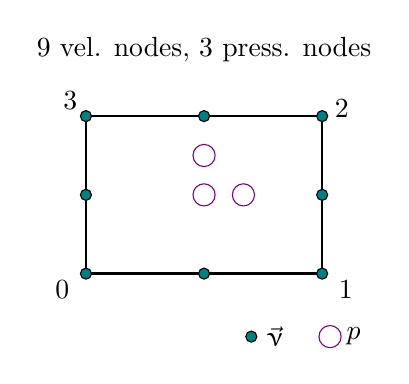
\begin{tikzpicture}
%\draw[fill=gray!23,gray!23](0,0) rectangle (5,5);
%\draw[step=0.5cm,gray,very thin] (0,0) grid (5,5); %background grid
\draw[thick] (1,1) -- (4,1) -- (4,3) -- (1,3) -- cycle;  
\node[] at (0.7,0.8) {0};
\node[] at (4.3,0.8) {1};
\node[] at (4.25,3.1) {2};
\node[] at (0.8,3.2) {3};
\draw[black,fill=teal] (1,1)     circle (2pt); 
\draw[black,fill=teal] (4,1)   circle (2pt); 
\draw[black,fill=teal] (4,3)   circle (2pt); 
\draw[black,fill=teal] (1,3) circle (2pt); 
\draw[black,fill=teal] (2.5,1) circle (2pt) ; 
\draw[black,fill=teal] (2.5,3) circle (2pt) ; 
\draw[black,fill=teal] (1,2) circle (2pt) ; 
\draw[black,fill=teal] (4,2) circle (2pt) ; 

\draw[violet] (2.5,2) circle (4pt);
\draw[violet] (3,2) circle (4pt);
\draw[violet] (2.5,2.5) circle (4pt);

\draw[black,fill=teal] (3.1,0.2) circle (2pt); 
\node[] at (3.4,0.2) {$\vec\upnu$};
\draw[violet] (4.1,0.2) circle (4pt); 
\node[] at (4.4,0.2) {$p$};
\node[] at (2.5,3.85) {9 vel. nodes, 3 press. nodes};
\end{tikzpicture}
%\end{center}

\end{center}

This element is crowned ``probably the most accurate 2D element'' in \textcite{grsa}.

It is characterised by piecewise bi/triquadratic velocities, 
and piecewise linear discontinuous polynomial pressure. 
The element satisfies the inf-sup condition, see p.~211 of \textcite{hugh}, or 
p.~138 of \textcite{elsw}.
It is used for example in \textcite{vavs89} (1989) for steady laminar flow in a curved tube
but also and more importantly it is the element pair used in \textcite{mabl15} (2015)
and it is available in \aspect too. 


When using this element one must be aware of the fact that there are 
two possible choices for the definitions of the pressure space 
(the so-called ``mapped'' and ``unmapped'' variants):

\textcite{bobf08} (2008) state: 
\begin{displayquote}
{\color{darkgray}
On a general quadrilateral mesh, the [pressure] space 
can be defined in two different ways: either [it] 
consists of (discontinuous) piecewise linear functions, or it is built
by considering three linear shape functions on the reference unit square and mapping
them to the general elements like it is usually done for continuous 
finite elements. [...] We shall refer to the first possibility as 
unmapped pressure approach and to the second one as mapped pressure approach.

[...] 

So far, we have shown that either the 
unmapped and the mapped pressure 
approach gives rise to a stable ${\bm Q}_2\times P_{-1}$ scheme. 
However, as a consequence of the
results proved in \textcite{arbf02} (2002), we have that the mapped 
pressure approach cannot achieve 
optimal approximation order. Namely, the unmapped pressure space 
provides a second-order convergence 
in $L_2$, while the mapped one achieves only ${\cal O}(h)$ in the same norm.}
\end{displayquote}

We also read in \textcite{boga02} (2002):
\begin{displayquote}
{\color{darkgray}
Two possible choices are given for the definition of the pressure space: 
one can either use a global pressure approximation (that is on
each quadrilateral the finite element space is spanned by 1 and by the 
global co-ordinates $x$ and $y$) or a local approach (consisting in generating 
the local space by means of the constants and the local curvilinear 
co-ordinates on each quadrilateral $r$ and $s$). [...] Numerical results 
actually show that the second choice (local or mapped pressure approximation) 
is suboptimally convergent.
}
\end{displayquote}

See also discussion about mapped/unmapped in \textcite{bobf13} and 
in Section 3.6.4 of \textcite{john16}.

This element is mentioned in \textcite{kaus10} (2010) and \textcite{pefc89} (1989) 
and it is used in \textcite{freh14} (2014) to study 3D fold growth rates 
(see online supplementary material) and in \textcite{schm08} (2008).

Note that the serendipity version of this pair, 
i.e. ${\bm Q}_2^{(20)}\times P_{-1}$ is also LBB stable
as shown in page 180 of Reddy's book \cite{reddybook2}.

{\color{red} since I wrote this I have purchased many relevant FE books
and I need to go through all and extract relevant facts and remarks about 
this element pair.}


%------------------------------------------------------------------------------
\subsection*{Deriving the mapped vs unmapped pressure basis functions}


The mapped version consists of  
using the $P_{-1}$ basis functions defined in Section~\ref{MMM-ss:lbfq2D}:
inside the reference cell the pressure is given by $p^h(r,s)=a+br+cs$.
The reference cell is the $[-1:1]^2$ square in the 2d Cartesian axis
system $r,s$.
Nodes are placed as follows: node 0 at (0,0), node 1 at (1/2,0) and node 2 at (0,1/2).

\begin{verbatim}
3--6--2   +-----+
|     |   |  2  |
7  8  5   +  01 |
|     |   |     |
0--4--1   +--+--+
V nodes   P nodes
\end{verbatim}

This yields the following basis functions
\begin{align}
\bN_0^p &= 1-2r-2s \nn\\
\bN_1^p &= 2r \nn\\
\bN_2^p &= 2s \nn
\end{align}
with 
\[
p^h(r,s) = \sum_{k=0}^2 \bN_k^p(r,s) \ p_k
\]
Obviously we recover $\sum\limits_{k=0}^2 \bN_k^p = 1$ and $\bN_k^p(r_i,s_i)=\delta_{ik}$.

W.B. adds:
\begin{displayquote}
{\color{darkgray}
[...] where to define the node functionals for the $P_{-1}$ space: It doesn't
matter. [...] In the end, you can
choose the three points however you like, they just can't all lie on a line
(in which case they would no longer uniquely describe the shape functions).

You place nodes on the reference cell, along midpoints of edges for
example. You then map these locations forward using whatever mapping you use. 
}
\end{displayquote}

The unmapped approach is a bit less straightforward and the procedure is as follows:
let us assume there are three distinct pressure nodes inside the cell (the 'real'
cell, not the reference cell).
Inside this cell the pressure is defined by a linear field
\[
p^h(x,y) = a+bx+cy
\]
We must then compute the coefficients $a,b,c$. We know that 
the expression above evaluated at the pressure nodes i=0,1,2 with 
coordinates $(x_i,y_i)$ should be equal to $p_i$. 
Then we have the following three equations:
\begin{eqnarray}
a + bx_0 + cy_0 &=& p_0 \nn\\
a + bx_1 + cy_1 &=& p_1 \nn\\
a + bx_2 + cy_2 &=& p_2 \nn
\end{eqnarray}
or, 
\[
\underbrace{
\left(
\begin{array}{ccc}
1 & x_0 & y_0 \\
1 & x_1 & y_1 \\
1 & x_2 & y_2 
\end{array}
\right)
}_{{\bm M}}
\cdot 
\left(
\begin{array}{ccc}
a \\ b \\ c
\end{array}
\right)
=
\underbrace{
\left(
\begin{array}{ccc}
p_0 \\ p_1 \\ p_2
\end{array}
\right)
}_{\vec{p}}
\]
Then 
\[
\left(
\begin{array}{ccc}
a \\ b \\ c
\end{array}
\right)
=
\left(
\begin{array}{ccc}
1 & x_0 & y_0 \\
1 & x_1 & y_1 \\
1 & x_2 & y_2 
\end{array}
\right)^{-1}
\cdot
\left(
\begin{array}{ccc}
p_0 \\ p_1 \\ p_2
\end{array}
\right)
= {\bm M}^{-1} \cdot \vec{p}
\]
with 
\[
{\bm M}^{-1} 
= {\bm N} 
= \frac{1}{\Delta}
\left(
\begin{array}{ccc}
x_1y_2-x_2y_1 & x_2y_0-x_0y_2 & x_0y_1-x_1y_0 \\
y_1-y_2 & y_2-y_0 & y_0-y_1 \\
x_2-x_1 & x_0-x_2 & x_1-x_0
\end{array}
\right)
%=
%\left(
%\begin{array}{ccc}
%n_{11} & n_{12} & n_{13} \\
%n_{21} & n_{22} & n_{23} \\
%n_{31} & n_{32} & n_{33} 
%\end{array}
%\right)
\]
and
\[
\Delta = x_1y_2-x_2y_1 - x_0y_2-x_2y_0 + x_0y_1-x_1y_0
\]
so that
\begin{eqnarray}
a &=& N_{11}p_0 + N_{12} p_1 + N_{13} p_2 \nn\\
b &=& N_{21}p_0 + N_{22} p_1 + N_{23} p_2 \nn\\
c &=& N_{31}p_0 + N_{32} p_1 + N_{33} p_2 \nn
\end{eqnarray}
In the end 
\begin{eqnarray}
p^h(x,y) 
&=&  a+bx+cy \nn\\
&=& N_{11}p_0 + N_{12} p_1 + N_{13} p_2
+ ( N_{21}p_0 + N_{22} p_1 + N_{23} p_2) x
+ ( N_{31}p_0 + N_{32} p_1 + N_{33} p_2) y \nn\\
&=& \underbrace{(N_{11} + N_{21}x + N_{31}y)}_{\bN_0^p(x,y)} p_0 
+   \underbrace{(N_{12} + N_{22}x + N_{32}y)}_{\bN_1^p(x,y)} p_1 
+   \underbrace{(N_{13} + N_{23}x + N_{33}y)}_{\bN_1^p(x,y)} p_2
%\label{f76_NNNP}
\end{eqnarray}
The basis functions are then evaluated at the (real) coordinates 
of the quadrature point $(x_q,y_q)$.

%{\color{red} Q1: is this the right/standard way of deriving these 
%basis functions? I suspect not. How is this carried out in deal.II?}

Actually it was pointed out by W.B. that 
{\color{darkgray} the unmapped basis $\{1,x,y\}$ is not good. That's because if you have a
small cell that is far away from the origin, the function $x$ varies very
little and so the function '$x$' is nearly constant on the cell -- so it is
almost collinear with the function '1'. You will see this in the fact
that the matrix ${\bm M}$ is nearly singular for such cells. 

A better choice is to use  $\{1, (x-x_c)/h, (y-y_c)/h \}$
where $h$ is some kind of cell diameter and $x_c,y_c$ are the cell center, 
or one of the vertices, or some such. The space is obviously the same.}

In light of this pertinent remark\footnote{duh...}, let us then start again from 
\[
p^h(x,y) = a+b\frac{x-x_c}{h}+c \frac{y-y_c}{h}
\]
leading to write:
\begin{eqnarray}
a + b \frac{x_0-x_c}{h} + c\frac{y_0-y_c}{h} &=& p_0 \nn\\
a + b \frac{x_1-x_c}{h} + c\frac{y_1-y_c}{h} &=& p_1 \nn\\
a + b \frac{x_2-x_c}{h} + c\frac{y_2-y_c}{h} &=& p_2 \nn
\end{eqnarray}
We then define $\tilde{x}_i=(x_i-x_c)/h$ and $\tilde{y}_i=(y_i-x_c)/h$ so that 
the equation above simply becomes
\begin{eqnarray}
a + b\tilde{x}_0 + c\tilde{y}_0 &=& p_0 \nn\\
a + b\tilde{x}_1 + c\tilde{y}_1 &=& p_1 \nn\\
a + b\tilde{x}_2 + c\tilde{y}_2 &=& p_2 \nn
\end{eqnarray}
or
\[
\underbrace{
\left(\begin{array}{ccc}
1 & \tilde{x}_0 & \tilde{y}_0 \\
1 & \tilde{x}_1 & \tilde{y}_1 \\
1 & \tilde{x}_2 & \tilde{y}_2 
\end{array}\right)
}_{{\bm M}}
\cdot 
\left(\begin{array}{ccc}
a \\ b \\ c
\end{array}\right)
=
\underbrace{
\left(\begin{array}{ccc}
p_0 \\ p_1 \\ p_2
\end{array}\right)
}_{\vec{p}}
\qquad
\Rightarrow
\qquad
\left(\begin{array}{ccc}
a \\ b \\ c
\end{array}\right)
=
{\bm M}^{-1} \cdot \vec{p}
\]
with
\[
{\bm M}^{-1} 
= {\bm N} 
= \frac{1}{\Delta}
\left(
\begin{array}{ccc}
\tilde{x}_1y_2-\tilde{x}_2\tilde{y}_1 
& \tilde{x}_2\tilde{y}_0-\tilde{x}_0\tilde{y}_2 
& \tilde{x}_0\tilde{y}_1-\tilde{x}_1\tilde{y}_0 \\
\tilde{y}_1-\tilde{y}_2 & \tilde{y}_2-\tilde{y}_0 & \tilde{y}_0-\tilde{y}_1 \\
\tilde{x}_2-\tilde{x}_1 & \tilde{x}_0-\tilde{x}_2 & \tilde{x}_1-\tilde{x}_0
\end{array}
\right)
\]
and
\[
\Delta 
= \tilde{x}_1\tilde{y}_2-\tilde{x}_2\tilde{y}_1 
- \tilde{x}_0\tilde{y}_2-\tilde{x}_2\tilde{y}_0 
+ \tilde{x}_0\tilde{y}_1-\tilde{x}_1\tilde{y}_0
\]
so that
\begin{eqnarray}
a &=& N_{11}p_0 + N_{12} p_1 + N_{13} p_2 \nn\\
b &=& N_{21}p_0 + N_{22} p_1 + N_{23} p_2 \nn\\
c &=& N_{31}p_0 + N_{32} p_1 + N_{33} p_2 \nn
\end{eqnarray}
In the end
\begin{eqnarray}
p^h(x,y) %\nn\\
&=& a+b\frac{x-x_c}{h}+c \frac{y-y_c}{h} \nn\\
&=& (N_{11}p_0 + N_{12} p_1 + N_{13} p_2)
+ ( N_{21}p_0 + N_{22} p_1 + N_{23} p_2) \frac{x-x_c}{h}
+ ( N_{31}p_0 + N_{32} p_1 + N_{33} p_2) \frac{y-y_c}{h} \nn\\
&=&\underbrace{\left(N_{11} + N_{21} \frac{x-x_c}{h} + N_{31}\frac{y-y_c}{h}\right)}_{\bN_0^p(x,y)} p_0 \nn\\
&+&  \underbrace{\left(N_{12} + N_{22} \frac{x-x_c}{h} + N_{32}\frac{y-y_c}{h}\right)}_{\bN_1^p(x,y)} p_1 \nn\\
&+&  \underbrace{\left(N_{13} + N_{23} \frac{x-x_c}{h} + N_{33}\frac{y-y_c}{h}\right)}_{\bN_1^p(x,y)} p_2
\label{f76_NNNP}
\end{eqnarray}

The pressure basis functions are then 
\begin{align}
\bN_0^p(x,y) &= N_{11} + N_{21}\frac{x-x_c}{h}  + N_{31}\frac{y-y_c}{h} \nn\\
\bN_1^p(x,y) &= N_{12} + N_{22}\frac{x-x_c}{h}  + N_{32}\frac{y-y_c}{h} \nn\\
\bN_2^p(x,y) &= N_{13} + N_{23}\frac{x-x_c}{h}  + N_{33}\frac{y-y_c}{h} \nn
\end{align}

In practice we will set 
\[
x_c=\frac14(x_0+x_1+x_2+x_3)
\qquad
y_c=\frac14(y_0+y_1+y_2+y_3)
\]
The function which computes the $N_{ij}$ coefficients is as follows:
\begin{lstlisting}
def compute_Ncoeffs(x0,x1,x2,y0,y1,y2,xxc,yyc,hh):
    xx0=(x0-xxc)/hh ; yy0=(y0-yyc)/hh
    xx1=(x1-xxc)/hh ; yy1=(y1-yyc)/hh
    xx2=(x2-xxc)/hh ; yy2=(y2-yyc)/hh
    det=xx1*yy2-xx2*yy1 -xx0*yy2-xx2*yy0 +xx0*yy1-xx1*yy0
    N11=(xx1*yy2-xx2*yy1)/det ; N12=(xx2*yy0-xx0*yy2)/det ; N13=(xx0*yy1-xx1*yy0)/det
    N21=(yy1-yy2        )/det ; N22=(yy2-yy0        )/det ; N23=(yy0-yy1        )/det
    N31=(xx2-xx1        )/det ; N32=(xx0-xx2        )/det ; N33=(xx1-xx0        )/det
    return N11,N12,N13,N21,N22,N23,N31,N32,N33 
\end{lstlisting}



%------------------------------------------------------------------------------
\subsection*{About the code}


The 2d $Q_2$ shape functions have been derived in Section~\ref{MMM-ss:q22d}
and the internal numbering of velocity nodes is as follows:
\begin{verbatim}
3--6--2
|     |
7  8  5
|     |
0--4--1
\end{verbatim}

For all the tests/benchmarks the domain is a unit square.
Velocity nodes coordinates are stored in the \lstinline{xV,yV} arrays
with the \lstinline{iconV} connectivity array.
Pressure nodes coordinates are stored in the \lstinline{xP,yP} arrays
with the \lstinline{iconP} connectivity array.
The mesh counts \lstinline{nel=nelx*nely} cells,
\lstinline{NV=(2*nelx+1)*(2*nely+1)} velocity nodes and 
\lstinline{NP=3*nel} pressure nodes.
The \lstinline{meth} parameter is 1 for mapped approach and 2 
for unmapped approach. 

Six types of meshes have been implemented so far: 
\begin{itemize}
\item \lstinline{mesh_type=1}:
The first type is straightforward: all cells are rectangular (and in 
practice square for simplicity).
\item \lstinline{mesh_type=2}:
The second type sees a random perturbation added to interior nodes.
The parameter \lstinline{xi} controls the randomness of the mesh as follows:
for each node inside the domain (i.e. not on the boundaries) a random value 
in the range $[-\xi,\xi]$ ($\xi$ is set to 0.1 by default) 
is added to the $x$ and $y$ coordonates:
\begin{lstlisting}
for i in range(0,NV):
    if xV[i]>0 and xV[i]<Lx and yV[i]>0 and yV[i]<Ly:
       xV[i]+=random.uniform(-1.,+1)*hx*xi
       yV[i]+=random.uniform(-1.,+1)*hy*xi
\end{lstlisting}
\item \lstinline{mesh_type=3}:
it is borrowed from \stone~25 which models the 
Rayleigh-Taylor experiment of \textcite{vaks97} (1997). Only the vertical position 
of the nodes is modified: nodes at about 1/5 the height of the domain are set to 
follow a sinusoidal perturbation and the position of other nodes above or below
is then adjusted as shown in the figure below. 

\item \lstinline{mesh_type=4}: after the regular square mesh 
is created the position of all nodes is moved with the following 
equations:
\begin{lstlisting}
for i in range(0,NV):
    yV[i]=(yV[i])**(0.75+xV[i]/4.)
    xV[i]=(xV[i])**(0.75+yV[i]/4.)
\end{lstlisting}
This results in a mesh with cells of various sizes, no right angle and no parallel edges
as shown hereafter.

\item \lstinline{mesh_type=5}: after the regular square mesh 
is created the position of all interior nodes is moved with the following
\begin{lstlisting}
for i in range(0,NV):
    if xV[i]>0 and xV[i]<1: 
       xV[i]+=np.sin(4*np.pi*yV[i])*hx/5
    if yV[i]>0 and yV[i]<1: 
       yV[i]+=np.sin(5*np.pi*xV[i])*hy/5
\end{lstlisting}
Again, this results in a mesh with cells of various sizes, no right angle and no parallel edges.
Note that the amplitude of the perturbation(s) is proportional to $h_x,h_y$ but not its wavelength.

\item \lstinline{mesh_type=6}: This mesh is composed of three
regular meshes that are glued together (ABED, BCGE, DEGF):
\begin{verbatim}
F--------G
|      / |
|    /   |
D--E     |
|   \    |
|    \   |
A-----B--C
\end{verbatim}
The idea behind this mesh to have a mesh with a different topology than the others, 
in this case E is a node that belongs to 3 cells instead of 4.
In the {\pythonfile tools.py} there are two functions:
\begin{itemize}
\item \verb'merge_two_blocks': it takes as arguments two meshes and returns a single mesh in which 
the overlapping nodes of both have been merged and the global numbering and connectivity array computed.
\item \verb'export_to_vtu': it takes a mesh and exports it to vtu format.
\end{itemize}
when \lstinline{nelx} is set by the bash script, all three blocks are then assigned a 
resolution \lstinline{nelx/2} $\times$ \lstinline{nelx/2} so that the resolution/cell size
on the left and bottom boundaries is the $h_x$ and $h_y$ values of the square mesh. 
The resulting mesh is shown hereunder. 
\end{itemize}

The six types of meshes are shown here:

\begin{center}
{\small 1})\includegraphics[width=5.5cm]{python_codes/fieldstone_76/results/mt1}
{\small 2})\includegraphics[width=5.5cm]{python_codes/fieldstone_76/results/mt2}
{\small 3})\includegraphics[width=5.5cm]{python_codes/fieldstone_76/results/mt3}\\
{\small 4})\includegraphics[width=5.5cm]{python_codes/fieldstone_76/results/mt4}
{\small 5})\includegraphics[width=5.5cm]{python_codes/fieldstone_76/results/mt5}
{\small 6})\includegraphics[width=5.5cm]{python_codes/fieldstone_76/results/mt6}\\
{\captionfont From left to right, top to bottom: mesh types 1, 2, 3, 4, 5 and 6, 
or 'square', 'randomized', 'wave', 'stretched', 'sin-sin' and 'glued' meshes.}
\end{center}

Looking at the meshes above we find that the cells of the 'wave' mesh 
can be obtained by affine transformation\footnote{\url{https://en.wikipedia.org/wiki/Affine_transformation}} 
of the reference cell (if straight edges are used -- see next paragraph) 
but not the cells of the 'randomized', 'stretched' and 'sin-sin' mesh. 
Quickly: an affine transformation 
is a geometric transformation that preserves lines and parallelism, but not necessarily 
Euclidean distances and angles. 
I remember coming across this terminology in the relevant literature (which I need to find again!)
and this may explain the results obtained for the manufactured solutions I ran the code on 
in what follows on both these types of meshes.

If the parameter \lstinline{straight_edges} is set to \lstinline{True}
the following algorithm makes sure that the velocity nodes 4,5,6,7 in the middle of the edges 
are really put back between nodes 0-1, 1-2, 2-3, and 3-0 respectively. 
\begin{lstlisting}
for iel in range(0,nel):
    xV[iconV[4,iel]]=0.5*(xV[iconV[0,iel]]+xV[iconV[1,iel]])
    yV[iconV[4,iel]]=0.5*(yV[iconV[0,iel]]+yV[iconV[1,iel]])
    xV[iconV[5,iel]]=0.5*(xV[iconV[1,iel]]+xV[iconV[2,iel]])
    yV[iconV[5,iel]]=0.5*(yV[iconV[1,iel]]+yV[iconV[2,iel]])
    xV[iconV[6,iel]]=0.5*(xV[iconV[2,iel]]+xV[iconV[3,iel]])
    yV[iconV[6,iel]]=0.5*(yV[iconV[2,iel]]+yV[iconV[3,iel]])
    xV[iconV[7,iel]]=0.5*(xV[iconV[3,iel]]+xV[iconV[0,iel]])
    yV[iconV[7,iel]]=0.5*(yV[iconV[3,iel]]+yV[iconV[0,iel]])
\end{lstlisting}
The placement of the middle node 8 is discussed in what follows.


The mapping is isoparametric (i.e. $Q_2$). The same mapping is used for changes 
of variables and for all integrals, Jacobians, etc ...
In the case of rectangular cells both the mapped and unmapped approaches 
yield the same pressure basis functions values at the quadrature points
so the measured errors are identical.
I suspected this is true for all cells obtained by affine transformation
from reference cell, to which my asking about this, W.B. added:
\begin{displayquote}
{\color{darkgray}
``Affine'' in essence means ``almost linear''. A linear transformation $f(x)$
satisfies $f(x+y) = f(x)+f(y)$ and  $f(\alpha x) = \alpha f(x)$
which in particular implies that $f(0)=0$. 
In finite-dimensional vector spaces, every linear transformation can be written as
$ f(x) = Ax $ with a matrix $A$. 

Affine transformations are of the form $f(x) = Ax + b$
which you need in the finite element context of affine transformations because
you don't just want to stretch or rotate cells, but you also want to translate
them from the reference coordinate system to wherever the cell is located in
real space.

If you have only rectangular cells (in fact, if they are parallelograms, of
which rectangles are a special case), then indeed the mapping is affine. The
shape functions in the mapped and unmapped case are different, but they span
the same space. (The shape functions are linear in both cases, but they are
scaled differently.) As a consequence, the solution is indeed the same. Like
you suggest in your question, this is going to be true for any affine
(=parallelogram) cell. It is because when you map linear basis functions with
an affine mapping, you end up with linear basis functions; the unmapped case
starts with linear shape functions in real space. 
}
\end{displayquote}

The same quadrature rule is used for $\K$ and $\G$ blocks (called $A$ and $B$ blocks 
respectively in the ASPECT literature).
I have explored the effect of the number of quadrature points on the solution, 
by testing for $2^2$, $3^2$ and $4^2$ quadrature points
as parameterized by the \lstinline{nqperdim} parameter.
I unsurprisingly found that a $2^2$ is not sufficient to exactly integrate the 
terms found in the $\K$ and $\G$ blocks, $3^2$ is standard, 
and $4^2$ is wasteful and did not yield any change in the results compared to $3^2$.

One critical aspect of the implementation is the location of the pressure nodes
in the real cell. The code takes the following approach:
\begin{enumerate}
\item For each cell compute the coordinates of the velocity nodes 0-7,
\item Apply modifications to the mesh (stretching, randomization, ...),
\item Set location of (middle) velocity node 8 (see next section),
\item Use $Q_2$ mapping to compute $x,y$ coordinates of pressure nodes.
\end{enumerate}


In both cases (mapped and unmapped) the pressure is discontinuous from cell to cell 
and this adds complexity in terms of exporting it to vtu format (and plotting with paraview). 
I then simply choose to export the value of the pressure in the middle of 
each cell\footnote{I should improve this in the future, but it is 
only a visualisation problem and does not influence results.
I know how to fix it, but this has low priority.}

%............................................................................
\subsubsection{About the position of the middle node}

We can think of multiple ways to come up with the `center' of the cell, 
i.e. the location of node 8.

\begin{verbatim}
3--6--2 
|     | 
7  8  5 
|     | 
0--4--1 
V nodes 
\end{verbatim}

In the code these different approaches are parameterized by means of the
\lstinline{center} variable:

\begin{itemize}
\item \lstinline{center=0}: The middle node coordinates are simply the 
average of the corner coordinates 
\begin{align}
x_8&=(x_0+x_1+x_2+x_3)/4 \nn\\
y_8&=(y_0+y_1+y_2+y_3)/4 \nn
\end{align}

\item \lstinline{center=1}: The middle coordinates are the average all the 
4 corners and 4 mid-edge nodes coordinates:

\begin{align}
x_8&=(x_0+x_1+x_2+x_3+x_4+x_5+x_6+x_7)/8 \nn\\
y_8&=(y_0+y_1+y_2+y_3+y_4+y_5+y_6+y_7)/8 \nn
\end{align}

\item \lstinline{center=2}: The middle coordinates are obtained via a 
weighed sum of the corner coordinates and the mid-edge nodes 
coordinates\footnote{I have no idea where this comes from but left it in nevertheless.}: 

\begin{align}
x_8&=(x_0+x_1+x_2+x_3+3x_4+3x_5+3x_6+3x_7)/16. \nn\\
y_8&=(y_0+y_1+y_2+y_3+3y_4+3y_5+3y_6+3y_7)/16. \nn
\end{align}

\item \lstinline{center=3}: This approach is a bit more complex than the previous ones.
We start by acknowledging that we know the coordinates of nodes 0-7 in the reference space $(r,s)$ 
and in the real space $(x,y)$ so one could then use a $Q_2^{(8)}$ mapping (i.e. 'serendipity' $Q_2$)
to place node 8.

In this case the basis functions for this mapping are defined in Section~\ref{MMM-sec:serendipity2D}:
\begin{eqnarray}
\bN_0(r,s)&=& \frac{1}{4}(1-r)(1-s)(-r-s-1) \nn\\
\bN_1(r,s)&=& \frac{1}{4}(1+r)(1-s)(r-s-1) \nn\\
\bN_2(r,s)&=& \frac{1}{4}(1+r)(1+s)(r+s-1) \nn\\
\bN_3(r,s)&=& \frac{1}{4}(1-r)(1+s)(-r+s-1) \nn\\
\bN_4(r,s)&=& \frac{1}{2}(1-r^2)(1-s)  \nn\\
\bN_5(r,s)&=& \frac{1}{2}(1+r)  (1-s^2)\nn\\
\bN_6(r,s)&=& \frac{1}{2}(1-r^2)(1+s)  \nn\\
\bN_7(r,s)&=& \frac{1}{2}(1-r)  (1-s^2) \nn
\end{eqnarray}

We would then compute the location of node 8 as follows (its $r,s$ coordinates are $0,0$): 
\begin{eqnarray}
x_8
&=& \sum_{i=0}^7 \bN_i (r_8,s_8) x_i \nn\\
&=& \sum_{i=1}^7 \bN_i (0,0) x_i \nn\\
&=& -\frac14 (x_0+x_1+x_2+x_3) + \frac12 (x_4+x_5+x_6+x_7) \nn\\
y_8 
&=& \sum_{i=0}^7 \bN_i (r_8,s_8) y_i \nn\\
&=& \sum_{i=0}^7 \bN_i (0,0) y_i \nn\\
&=& -\frac14 (y_0+y_1+y_2+y_3) + \frac12 (y_4+y_5+y_6+y_7) \nn
\end{eqnarray}

\end{itemize}

In the case of parallelogram cells these four approaches lead to the same 
middle location. This is no more the case for elements with curved edges
for example and therefore warrants a thorough study.

%--------------------------------------------------------------------------------------
\subsection*{The manufactured solutions}

Note that for all four manufactured solutions used in the present code 
a) the pressure obeys $\int_{\Omega} p \; dV = 0$;
b) the analytical velocity is prescribed on the boundary of the domain; 
c) the viscosity is 1 (except SolKz); d) the domain is the unit square. 

\begin{itemize}
\item {\tt bench=3}: 
This is the Donea \& Huerta benchmark that is fully described in Section~\ref{MMM-mms1}.
The velocity and pressure are given by
\begin{eqnarray}
u(x,y) &=& x^2(1-x)^2 2y (y-1)(2y-1) \\ 
v(x,y) &=& -y^2 (1 - y)^2 2x (x-1)(2x-1) \\ 
p(x,y) &=& x(1 -x)- 1/6 
\end{eqnarray}

\item {\tt bench=1}:  
The analytical solution originates in Lamichhane (2017) \cite{lami17}.
The velocity and pressure are given by
\begin{eqnarray}
u(x,y)&=&-2x^2y(2y-1)(x-1)^2(y-1) \\
v(x,y)&=& 2xy^2(2x-1)(x-1)(y-1)^2 \\
p(x,y)&=& x(1-x)(1-2y)
\end{eqnarray}
The corresponding body force terms are derived in Section~\ref{MMM-ss:mms11}. 

\item {\tt bench=9}: 
This is the second manufactured solution 
mentioned in Lamichhane \cite{lami17}. 
The velocity and pressure are given by
\begin{eqnarray}
u(x,y) &=& x+x^2 - 2xy+x^3 - 3xy^2 + x^2y \\
v(x,y) &=& -y-2xy+y^2 -3x^2y + y^3 - xy^2 \\
p(x,y) &=& xy+x+y+x^3y^2 - 4/3
\end{eqnarray}
The corresponding body force terms are derived in Section~\ref{MMM-ss:mms2}. 

\item {\tt bench=4}. This is the SolKz benchmark described in Section~\ref{MMM-ss:solkz}.
The main difference with respect to the previous three ones is the fact that the viscosity
varies by 6 orders of magnitude (albeit is a smooth manner).


\end{itemize}

The numbering {\tt bench=3,1,9,4} is completely arbitrary and inherited from another \stone.

In what follows velocity and pressure error convergence is measured as a function of
mesh side. Since for some meshes there is not a single obvious mesh size, 
I then use the square root of the maximum value of the elemental area array:
\[
h \simeq \sqrt{\max_e A_e }
\]


\newpage
%--------------------------------------------------------------------------------------
\subsection*{Manufactured solution of Donea \& Huerta ({\tt bench=3}) - straight edges}

\begin{center}
\includegraphics[width=6.5cm]{python_codes/fieldstone_76/results/bench3/straight/errors_V_mt1.pdf}
\includegraphics[width=6.5cm]{python_codes/fieldstone_76/results/bench3/straight/errors_P_mt1.pdf}\\
\includegraphics[width=6.5cm]{python_codes/fieldstone_76/results/bench3/straight/errors_V_mt2.pdf}
\includegraphics[width=6.5cm]{python_codes/fieldstone_76/results/bench3/straight/errors_P_mt2.pdf}\\
\includegraphics[width=6.5cm]{python_codes/fieldstone_76/results/bench3/straight/errors_V_mt3.pdf}
\includegraphics[width=6.5cm]{python_codes/fieldstone_76/results/bench3/straight/errors_P_mt3.pdf}\\
\includegraphics[width=6.5cm]{python_codes/fieldstone_76/results/bench3/straight/errors_V_mt4.pdf}
\includegraphics[width=6.5cm]{python_codes/fieldstone_76/results/bench3/straight/errors_P_mt4.pdf}\\
\includegraphics[width=6.5cm]{python_codes/fieldstone_76/results/bench3/straight/errors_V_mt5.pdf}
\includegraphics[width=6.5cm]{python_codes/fieldstone_76/results/bench3/straight/errors_P_mt5.pdf}\\
\includegraphics[width=6.5cm]{python_codes/fieldstone_76/results/bench3/straight/errors_V_mt6.pdf}
\includegraphics[width=6.5cm]{python_codes/fieldstone_76/results/bench3/straight/errors_P_mt6.pdf}\\
{\captionfont From top to bottom: square mesh, Randomized ($\xi=0.1$) mesh,
wave mesh, stretched mesh, sin-sin mesh and glued mesh.}
\end{center}

\newpage
%------------------------------------------------------------------------------------
\subsection*{Manufactured solution of Donea \& Huerta ({\tt bench=3}) - curved edges}

\begin{center}
\includegraphics[width=8cm]{python_codes/fieldstone_76/results/bench3/curved/errors_V_mt2.pdf}
\includegraphics[width=8cm]{python_codes/fieldstone_76/results/bench3/curved/errors_P_mt2.pdf}\\
\includegraphics[width=8cm]{python_codes/fieldstone_76/results/bench3/curved/errors_V_mt3.pdf}
\includegraphics[width=8cm]{python_codes/fieldstone_76/results/bench3/curved/errors_P_mt3.pdf}\\
\includegraphics[width=8cm]{python_codes/fieldstone_76/results/bench3/curved/errors_V_mt4.pdf}
\includegraphics[width=8cm]{python_codes/fieldstone_76/results/bench3/curved/errors_P_mt4.pdf}\\
\includegraphics[width=8cm]{python_codes/fieldstone_76/results/bench3/curved/errors_V_mt5.pdf}
\includegraphics[width=8cm]{python_codes/fieldstone_76/results/bench3/curved/errors_P_mt5.pdf}\\
{\captionfont From top to bottom: 'randomized' ($\xi=0.1$) mesh,
'wave' mesh, 'stretched' mesh and 'sin-sin' mesh.}
\end{center}

\newpage
%-----------------------------------------------------------------------
\subsection*{Manufactured solution \#1 ({\tt bench=1}) - straight edges}

\begin{center}
\includegraphics[width=6.5cm]{python_codes/fieldstone_76/results/bench1/straight/errors_V_mt1.pdf}
\includegraphics[width=6.5cm]{python_codes/fieldstone_76/results/bench1/straight/errors_P_mt1.pdf}\\
\includegraphics[width=6.5cm]{python_codes/fieldstone_76/results/bench1/straight/errors_V_mt2.pdf}
\includegraphics[width=6.5cm]{python_codes/fieldstone_76/results/bench1/straight/errors_P_mt2.pdf}\\
\includegraphics[width=6.5cm]{python_codes/fieldstone_76/results/bench1/straight/errors_V_mt3.pdf}
\includegraphics[width=6.5cm]{python_codes/fieldstone_76/results/bench1/straight/errors_P_mt3.pdf}\\
\includegraphics[width=6.5cm]{python_codes/fieldstone_76/results/bench1/straight/errors_V_mt4.pdf}
\includegraphics[width=6.5cm]{python_codes/fieldstone_76/results/bench1/straight/errors_P_mt4.pdf}\\
\includegraphics[width=6.5cm]{python_codes/fieldstone_76/results/bench1/straight/errors_V_mt5.pdf}
\includegraphics[width=6.5cm]{python_codes/fieldstone_76/results/bench1/straight/errors_P_mt5.pdf}\\
\includegraphics[width=6.5cm]{python_codes/fieldstone_76/results/bench1/straight/errors_V_mt6.pdf}
\includegraphics[width=6.5cm]{python_codes/fieldstone_76/results/bench1/straight/errors_P_mt6.pdf}\\
{\captionfont From top to bottom: 'square mesh', 'randomized' ($\xi=0.1$) mesh,
'wave' mesh, 'stretched' mesh, 'sin-sin' mesh and 'glued' mesh.}
\end{center}

\newpage
%.......................................................................
\subsection*{Manufactured solution \#1 ({\tt bench=1}) - curved edges}

\begin{center}
\includegraphics[width=8cm]{python_codes/fieldstone_76/results/bench1/curved/errors_V_mt2.pdf}
\includegraphics[width=8cm]{python_codes/fieldstone_76/results/bench1/curved/errors_P_mt2.pdf}\\
\includegraphics[width=8cm]{python_codes/fieldstone_76/results/bench1/curved/errors_V_mt3.pdf}
\includegraphics[width=8cm]{python_codes/fieldstone_76/results/bench1/curved/errors_P_mt3.pdf}\\
\includegraphics[width=8cm]{python_codes/fieldstone_76/results/bench1/curved/errors_V_mt4.pdf}
\includegraphics[width=8cm]{python_codes/fieldstone_76/results/bench1/curved/errors_P_mt4.pdf}\\
\includegraphics[width=8cm]{python_codes/fieldstone_76/results/bench1/curved/errors_V_mt5.pdf}
\includegraphics[width=8cm]{python_codes/fieldstone_76/results/bench1/curved/errors_P_mt5.pdf}\\
{\captionfont From top to bottom: 'randomized' ($\xi=0.1$) mesh,
'wave' mesh, 'stretched' mesh and 'sin-sin' mesh.}
\end{center}


\newpage
%.......................................................................
\subsection*{Manufactured solution \#2 ({\tt bench=9}) - straight edges}

\begin{center}
\includegraphics[width=6.5cm]{python_codes/fieldstone_76/results/bench9/straight/errors_V_mt1.pdf}
\includegraphics[width=6.5cm]{python_codes/fieldstone_76/results/bench9/straight/errors_P_mt1.pdf}\\
\includegraphics[width=6.5cm]{python_codes/fieldstone_76/results/bench9/straight/errors_V_mt2.pdf}
\includegraphics[width=6.5cm]{python_codes/fieldstone_76/results/bench9/straight/errors_P_mt2.pdf}\\
\includegraphics[width=6.5cm]{python_codes/fieldstone_76/results/bench9/straight/errors_V_mt3.pdf}
\includegraphics[width=6.5cm]{python_codes/fieldstone_76/results/bench9/straight/errors_P_mt3.pdf}\\
\includegraphics[width=6.5cm]{python_codes/fieldstone_76/results/bench9/straight/errors_V_mt4.pdf}
\includegraphics[width=6.5cm]{python_codes/fieldstone_76/results/bench9/straight/errors_P_mt4.pdf}\\
\includegraphics[width=6.5cm]{python_codes/fieldstone_76/results/bench9/straight/errors_V_mt5.pdf}
\includegraphics[width=6.5cm]{python_codes/fieldstone_76/results/bench9/straight/errors_P_mt5.pdf}\\
\includegraphics[width=6.5cm]{python_codes/fieldstone_76/results/bench9/straight/errors_V_mt6.pdf}
\includegraphics[width=6.5cm]{python_codes/fieldstone_76/results/bench9/straight/errors_P_mt6.pdf}\\
{\captionfont From top to bottom: 'square' mesh, 'randomized' ($\xi=0.1$) mesh,
'wave' mesh, 'stretched' mesh, 'sin-sin' mesh and 'glued' mesh.}
\end{center}

\newpage
%.......................................................................
\subsection*{Manufactured solution \#2 ({\tt bench=9}) - curved edges}

\begin{center}
\includegraphics[width=8cm]{python_codes/fieldstone_76/results/bench9/curved/errors_V_mt2.pdf}
\includegraphics[width=8cm]{python_codes/fieldstone_76/results/bench9/curved/errors_P_mt2.pdf}\\
\includegraphics[width=8cm]{python_codes/fieldstone_76/results/bench9/curved/errors_V_mt3.pdf}
\includegraphics[width=8cm]{python_codes/fieldstone_76/results/bench9/curved/errors_P_mt3.pdf}\\
\includegraphics[width=8cm]{python_codes/fieldstone_76/results/bench9/curved/errors_V_mt4.pdf}
\includegraphics[width=8cm]{python_codes/fieldstone_76/results/bench9/curved/errors_P_mt4.pdf}\\
\includegraphics[width=8cm]{python_codes/fieldstone_76/results/bench9/curved/errors_V_mt5.pdf}
\includegraphics[width=8cm]{python_codes/fieldstone_76/results/bench9/curved/errors_P_mt5.pdf}\\
{\captionfont From top to bottom: 'randomized' ($\xi=0.1$) mesh,
'wave' mesh, 'stretched' mesh and 'sin-sin' mesh.}
\end{center}


\newpage
%.......................................................................
\subsection*{Manufactured solution SolKz ({\tt bench=4}) - straight edges}

\begin{center}
\includegraphics[width=6.5cm]{python_codes/fieldstone_76/results/bench4/straight/errors_V_mt1.pdf}
\includegraphics[width=6.5cm]{python_codes/fieldstone_76/results/bench4/straight/errors_P_mt1.pdf}\\
\includegraphics[width=6.5cm]{python_codes/fieldstone_76/results/bench4/straight/errors_V_mt2.pdf}
\includegraphics[width=6.5cm]{python_codes/fieldstone_76/results/bench4/straight/errors_P_mt2.pdf}\\
\includegraphics[width=6.5cm]{python_codes/fieldstone_76/results/bench4/straight/errors_V_mt3.pdf}
\includegraphics[width=6.5cm]{python_codes/fieldstone_76/results/bench4/straight/errors_P_mt3.pdf}\\
\includegraphics[width=6.5cm]{python_codes/fieldstone_76/results/bench4/straight/errors_V_mt4.pdf}
\includegraphics[width=6.5cm]{python_codes/fieldstone_76/results/bench4/straight/errors_P_mt4.pdf}\\
\includegraphics[width=6.5cm]{python_codes/fieldstone_76/results/bench4/straight/errors_V_mt5.pdf}
\includegraphics[width=6.5cm]{python_codes/fieldstone_76/results/bench4/straight/errors_P_mt5.pdf}\\
\includegraphics[width=6.5cm]{python_codes/fieldstone_76/results/bench4/straight/errors_V_mt6.pdf}
\includegraphics[width=6.5cm]{python_codes/fieldstone_76/results/bench4/straight/errors_P_mt6.pdf}\\
{\captionfont From top to bottom: 'square' mesh, 'randomized' ($\xi=0.1$) mesh,
'wave' mesh, 'stretched' mesh, 'sin-sin' mesh and 'glued' mesh.}
\end{center}

\newpage
%.......................................................................
\subsection*{Manufactured solution SolKz ({\tt bench=4}) - curved edges}

\begin{center}
\includegraphics[width=8cm]{python_codes/fieldstone_76/results/bench4/curved/errors_V_mt2.pdf}
\includegraphics[width=8cm]{python_codes/fieldstone_76/results/bench4/curved/errors_P_mt2.pdf}\\
\includegraphics[width=8cm]{python_codes/fieldstone_76/results/bench4/curved/errors_V_mt3.pdf}
\includegraphics[width=8cm]{python_codes/fieldstone_76/results/bench4/curved/errors_P_mt3.pdf}\\
\includegraphics[width=8cm]{python_codes/fieldstone_76/results/bench4/curved/errors_V_mt4.pdf}
\includegraphics[width=8cm]{python_codes/fieldstone_76/results/bench4/curved/errors_P_mt4.pdf}\\
\includegraphics[width=8cm]{python_codes/fieldstone_76/results/bench4/curved/errors_V_mt5.pdf}
\includegraphics[width=8cm]{python_codes/fieldstone_76/results/bench4/curved/errors_P_mt5.pdf} \\
{\captionfont From top to bottom: 'randomized' ($\xi=0.1$) mesh,
'wave' mesh, 'stretched' mesh and 'sin-sin' mesh.}
\end{center}


%%%%%%%%%%%%%%%%%%%%%%%%%%%%%%%%%%%%%%%%%%%%%%%%%%%%%%%%%%%%%%%%%%%%%%%%%%%%%%%%%%%%%%%%%%%%%
\newpage
\subsection*{A recap of all convergence rates so far}


As mentioned for example in \textcite{thba25} (2025), 
one expects a 3rd-order convergence (in the $L_2$ norm) for the velocity
error and a 2nd-order convergence for the pressure error.
In the tables below error rates that are not the expect 3/2 are highlighted in bold.

Since all four \lstinline{center} approaches are identical for straight edges
cells I will then only report values for \lstinline{center=0}. 



\begin{center}
\includegraphics[width=2.7cm]{python_codes/fieldstone_76/results/mt1}
\includegraphics[width=2.7cm]{python_codes/fieldstone_76/results/mt2}
\includegraphics[width=2.7cm]{python_codes/fieldstone_76/results/mt3}
\includegraphics[width=2.7cm]{python_codes/fieldstone_76/results/mt4}
\includegraphics[width=2.7cm]{python_codes/fieldstone_76/results/mt5}
\includegraphics[width=2.7cm]{python_codes/fieldstone_76/results/mt6}\\
{\captionfont 'square' ,'random', 'wave', 'stretched', 'sin-sin', 'glued'.}
\end{center}

\begin{itemize}

%...................................
\item {\tt bench=3}

\begin{tabular}{c|cccccc}
\hline
straight& mt=1     &  mt=2        &  mt=3  &  mt=4       & mt=5  & mt=6\\
edges& 'square' & 'randomized' & 'wave' & 'stretched' & 'sin-sin' & 'glued'\\
\hline
mapped   & 3/2 & {\bf 2/1} &3/2 & {\bf 2.74/1.88} &3/2 \\
unmapped & 3/2 &3/2 &3/2 & {\bf 2.74/1.92} &3/2 \\
\hline
\end{tabular}

\begin{tabular}{c|cccc}
\hline
curved &  mt=2        &  mt=3  &  mt=4       & mt=5 \\
edges & 'randomized' & 'wave' & 'stretched' & 'sin-sin' \\
\hline
mapped   & \\ 
unmapped &  \\
\hline
\end{tabular}


%..........................
\item {\tt bench=1}

\begin{tabular}{c|cccccc}
\hline
straight & mt=1     &  mt=2        &  mt=3  &  mt=4       & mt=5  & mt=6\\
edges    & 'square' & 'randomized' & 'wave' & 'stretched' & 'sin-sin' & 'glued'\\
\hline
mapped   & 3/2 & {\bf 2/1} &3/2 & {\bf 2.74/1.88} &3/2 \\
unmapped & 3/2 &3/2 &3/2 & {\bf 2.74/1.92} &3/2 \\
\hline
\end{tabular}

\begin{tabular}{c|cccc}
\hline
curved&  mt=2        &  mt=3  &  mt=4       & mt=5 \\
edges& 'randomized' & 'wave' & 'stretched' & 'sin-sin' \\
\hline
mapped   & \\ 
unmapped &  \\
\hline
\end{tabular}

%...................................
\item {\tt bench=9}

\begin{tabular}{c|cccccc}
\hline
straight& mt=1     &  mt=2        &  mt=3  &  mt=4       & mt=5  & mt=6\\
edges& 'square' & 'randomized' & 'wave' & 'stretched' & 'sin-sin' & 'glued'\\
\hline
mapped   & 3/2 & {\bf 2/1} &3/2 & {\bf 2.78/1.98}  &3/2 \\
unmapped & 3/2 &3/2 &3/2 & {\bf 2.78/1.98} &3/2 \\
\hline
\end{tabular}


\begin{tabular}{c|cccc}
\hline
curved&  mt=2        &  mt=3  &  mt=4       & mt=5 \\
edges& 'randomized' & 'wave' & 'stretched' & 'sin-sin' \\
\hline
mapped   & \\ 
unmapped &  \\
\hline
\end{tabular}

%...................................
\item {\tt bench=4}

\begin{tabular}{c|cccccc}
\hline
straight& mt=1     &  mt=2        &  mt=3  &  mt=4       & mt=5  & mt=6\\
edges& 'square' & 'randomized' & 'wave' & 'stretched' & 'sin-sin' & 'glued'\\
\hline
mapped   & 3/2 & {\bf 2/1} &3/2 & {\bf 2.78/1.98}  &3/2 \\
unmapped & 3/2 &3/2 &3/2 & {\bf 2.78/1.98} &3/2 \\
\hline
\end{tabular}

\begin{tabular}{c|cccc}
\hline
curved&  mt=2        &  mt=3  &  mt=4       & mt=5 \\
edges& 'randomized' & 'wave' & 'stretched' & 'sin-sin' \\
\hline
mapped   & \\ 
unmapped &  \\
\hline
\end{tabular}

\end{itemize}

The clear conclusion from all this is that only \lstinline{center=0}
yields a pressure error which decreases monotonically with resolution 
for cells with curved edges. 

Note that for the stretched mesh the value of the parameter $h$ is not well defined (or
not as well defined as the other meshes). Since the $h$ value I use for these is overestimating
the size of the smallest cell, these could explain the slightly anomalous rates.

\newpage
%----------------------------------------
\subsection*{Instantaneous sinking block}

It is fully described in Section~\ref{MMM-ss:sinking_block}.
The block is centered in the domain, its density is 1\% larger than the 
fluid density ($\rho_f=1$) and its viscosity is 1000 times larger than 
the fluid viscosity ($\eta_f=1$).
The block is a square of dimension 1/8 so that using square meshes $16^2$, 
$32^2$, $48^2$, $64^2$, ... ensures that element edges align with the 
sides of the block.
Free-slip boundary conditions are prescribed on all sides.
This is not a benchmark {\it stricto sensu} as there is no analytical solution
available. 
Mesh type 1 is used (square elements) with resolutions $16^2, 32^2, 64^2, 96^2, 128^2, 192^2, 256^2$.

\begin{center}
\includegraphics[width=5cm]{python_codes/fieldstone_76/results/block/vel}
\includegraphics[width=5cm]{python_codes/fieldstone_76/results/block/press}\\
{\captionfont Velocity and pressure fields.}
\end{center}

The root mean square velocity and the maximum velocity in the domain are 
measured on a series of meshes 
and is shown on the following figure for both mapped and unmapped approaches: 

\begin{center}
\includegraphics[width=6cm]{python_codes/fieldstone_76/results/block/vrms.pdf}
\includegraphics[width=6cm]{python_codes/fieldstone_76/results/block/maxvel.pdf}
\end{center}

We find that the highest resolution $256^2$ is not high enough to yield a resolution-independent
measurement (although we note that the measurements above do not vary by more than 1\%). 

The velocity and pressure are measured on a vertical line passing through the 
middle of the block:

\begin{center}
\includegraphics[width=5.7cm]{python_codes/fieldstone_76/results/block/profile_m1_u.pdf}
\includegraphics[width=5.7cm]{python_codes/fieldstone_76/results/block/profile_m1_v.pdf}
\includegraphics[width=5.7cm]{python_codes/fieldstone_76/results/block/profile_m1_p.pdf}\\
\includegraphics[width=5.7cm]{python_codes/fieldstone_76/results/block/profile_m2_u.pdf}
\includegraphics[width=5.7cm]{python_codes/fieldstone_76/results/block/profile_m2_v.pdf}
\includegraphics[width=5.7cm]{python_codes/fieldstone_76/results/block/profile_m2_p.pdf}\\
{\captionfont The grey band indicates the $y$ values inside the block.}
\end{center}

Because of symmetry we expect and recover $u\simeq =0$ on this line.
The $v$-component seems to converge to a resolution independent profile
while the pressure is clearly dominated by the hydrostatic pressure.
We do not observe any difference between mapped and unmapped, as expected
since elements are square.

\newpage
%--------------------------------------------------------------
\subsection*{Instantaneous sinking block (reduced densities)}

The setup is identical to the previous one, except that now the fluid density is zero and 
the block density is 0.01. In other words the hydrostatic pressure has been removed.
We expect an identical velocity field but the recovered pressure is now the 
dynamic/excess pressure:

\begin{center}
\includegraphics[width=5.7cm]{python_codes/fieldstone_76/results/block_rd/profile_m1_u.pdf}
\includegraphics[width=5.7cm]{python_codes/fieldstone_76/results/block_rd/profile_m1_v.pdf}
\includegraphics[width=5.7cm]{python_codes/fieldstone_76/results/block_rd/profile_m1_p.pdf}\\
\includegraphics[width=5.7cm]{python_codes/fieldstone_76/results/block_rd/profile_m2_u.pdf}
\includegraphics[width=5.7cm]{python_codes/fieldstone_76/results/block_rd/profile_m2_v.pdf}
\includegraphics[width=5.7cm]{python_codes/fieldstone_76/results/block_rd/profile_m2_p.pdf}\\
{\captionfont The grey band indicates the $y$ values inside the block.}
\end{center}

We find that results obtained with ASPECT nicely agree with the results of this \stone.

\begin{center}
\includegraphics[width=8cm]{python_codes/fieldstone_76/results/block_rd/vrms.pdf}
\includegraphics[width=8cm]{python_codes/fieldstone_76/results/block_rd/maxvel.pdf}
\end{center}

\begin{center}
\includegraphics[width=5.7cm]{python_codes/fieldstone_76/results/block_rd/u}
\includegraphics[width=5.7cm]{python_codes/fieldstone_76/results/block_rd/v}
\includegraphics[width=5.7cm]{python_codes/fieldstone_76/results/block_rd/press}\\
{\captionfont Velocity and pressure fields on $96\times 96$ mesh. 
Note that the visualised pressure is elemental instead of $P_{-1}$.}
\end{center}







 %%%%%%%%%%%%%%%%%%%%%%%%%%%%%%%%%%%%%%%%%%%%%%%%%%%%%%%%%%%

\chapter{Rotated $Q_1\times P_0$ element \& DSSY element \label{f77}} %%%%%%%%%%%%%%%%%%%%%%%%%%%%% 77
\lstinputlisting[language=bash,basicstyle=\small]{python_codes/fieldstone_77/keywords.ascii}

\begin{center}
Code at \url{https://github.com/cedrict/fieldstone/tree/master/python_codes/fieldstone_77}
\end{center}

\par\noindent\rule{\textwidth}{0.4pt}

%%%%%%%%%%%%%%%%%%%%%%%%%%%%%%%%%%%%%%%%%%%%%%%%%%%%%%%%%%%%%%%%%%%%%%%%%%%%%%%%%%%%%%%%%%%%

I have implemented the two variants of the Rannacher-Turek element presented
in Section~\ref{ss:RTq1p0}, the mid-value (MV) and the mid-point (MP).
After communicating with Prof. Turek, I also implemented the Laplace 
formulation of the Stokes equation, i.e. we assume $\eta$ to be constant 
and therefore for an incompressible flow the momentum conservation 
equation becomes 
\[
-\vec\nabla p + \eta \Delta \vec\upnu + \rho \vec{g} = \vec{0}
\]
This yields a different form of the viscous block of the Stokes system
as explained in Section~\ref{ss:isovisc}.
I use an isoparametric mapping, but I have tried a $Q_1$ mapping and given that 
all elements are square it does not change anything. 

Following a discussion with W. Bangerth, I have also implemented the DSSY element 
(see Section~\ref{ss:dssy_2D}) which 'lives' on the same four nodes placed at 
the mid-edges. DSSY(1) corresponds to the basis functions based on $\theta_1$ 
while DSSY(2) corresponds to the basis functions based on $\theta_2$ \cite{doss99}

In what follows formulation 1 stands for the regular form of the 
Stokes equation, while formulation 2 stands for the Laplace one.

I have implemented four benchmarks based on manufactured solutions:
\begin{itemize}
\item Donea-Huerta, see Section~\ref{mms1}

\begin{center}
\includegraphics[width=7cm]{python_codes/fieldstone_77/results/dh/vel}
\includegraphics[width=7cm]{python_codes/fieldstone_77/results/dh/press}\\
\includegraphics[width=8cm]{python_codes/fieldstone_77/results/dh/errors_form1}
\includegraphics[width=8cm]{python_codes/fieldstone_77/results/dh/errors_form2}\\
\includegraphics[width=8cm]{python_codes/fieldstone_77/results/dh/vrms_form1}
\includegraphics[width=8cm]{python_codes/fieldstone_77/results/dh/vrms_form2}\\
\includegraphics[width=8cm]{python_codes/fieldstone_77/results/dh/vrms_form1_relerror}
\includegraphics[width=8cm]{python_codes/fieldstone_77/results/dh/vrms_form2_relerror}\\
{\captionfont Top row: Velocity and pressure error convergence; 
Middle row: root mean square velocity. 
Bottom row: root mean square velocity relative error.}
\end{center}

\item Volker John benchmark \cite{jolm17}, see Section~\ref{ss:mms_jolm17}:

\begin{center}
\includegraphics[width=7cm]{python_codes/fieldstone_77/results/vj/vel}
\includegraphics[width=7cm]{python_codes/fieldstone_77/results/vj/press}\\
\includegraphics[width=8cm]{python_codes/fieldstone_77/results/vj/errors_form1}
\includegraphics[width=8cm]{python_codes/fieldstone_77/results/vj/errors_form2}\\
\includegraphics[width=8cm]{python_codes/fieldstone_77/results/vj/vrms_form1}
\includegraphics[width=8cm]{python_codes/fieldstone_77/results/vj/vrms_form2}\\
\includegraphics[width=8cm]{python_codes/fieldstone_77/results/vj/vrms_form1_relerror}
\includegraphics[width=8cm]{python_codes/fieldstone_77/results/vj/vrms_form2_relerror}\\
{\captionfont Top row: Velocity and pressure error convergence; 
Middle row: root mean square velocity. 
Bottom row: root mean square velocity relative error.}
\end{center}

\item Dohrmann \& Bochev 2D benchmark \cite{dobo04,bodg06}, see Section~\ref{ss:mms2}:

\begin{center}
\includegraphics[width=7cm]{python_codes/fieldstone_77/results/db2D/vel}
\includegraphics[width=7cm]{python_codes/fieldstone_77/results/db2D/press}\\
\includegraphics[width=8cm]{python_codes/fieldstone_77/results/db2D/errors_form1}
\includegraphics[width=8cm]{python_codes/fieldstone_77/results/db2D/errors_form2}\\
\includegraphics[width=8cm]{python_codes/fieldstone_77/results/db2D/vrms_form1}
\includegraphics[width=8cm]{python_codes/fieldstone_77/results/db2D/vrms_form2}\\
\includegraphics[width=8cm]{python_codes/fieldstone_77/results/db2D/vrms_form1_relerror}
\includegraphics[width=8cm]{python_codes/fieldstone_77/results/db2D/vrms_form2_relerror}\\
{\captionfont Top row: Velocity and pressure error convergence; 
Middle row: root mean square velocity. 
Bottom row: root mean square velocity relative error.
Formulation 1 stands for the regular form of the 
Stokes equation, while formulation 2 stands for the Laplace one.}
\end{center}

\item SolCx benchmark, see \stone 5 (only formulation 1):

\begin{center}
\includegraphics[width=7cm]{python_codes/fieldstone_77/results/solcx/vel}
\includegraphics[width=7cm]{python_codes/fieldstone_77/results/solcx/press}\\
\includegraphics[width=8cm]{python_codes/fieldstone_77/results/solcx/errors_form1}
\includegraphics[width=8cm]{python_codes/fieldstone_77/results/solcx/vrms_form1}\\
{\captionfont Only even numbers of elements. Note that the paraview visualisation is based on 
quadrilaterals obtained by joining the nodes.}
\end{center}


\end{itemize}


Looking at these 4 analytical benchmarks (and focusing on the standard formulation only), 
we can conclude that RT(MV) and DSSY(1) are the two best elements and that they are very close to 
each other.



%........................................................................
\subsubsection*{Buoyancy-driven flow}

We see that both RT(MV) and DSSY(1) exhibit a quadratic convergence for the
velocity error and a linear convergence for the pressure error. Also the root mean square 
velocity measurements logically converge to their analytical values.  

Since these elements have been proven to be LBB stable one could think that it 
should then replace the standard $Q_1 \times P_0$: near identical cost, but LBB stable.

However, there is  a problem. I have also implemented another experiment: a unit cube domain
filled with a fluid of density $\rho_0=1$ and a cube of size $0.125\times 0.125$ centered in the domain
with density $\rho_0+\delta \rho$ with $\delta\rho=0.01$. The fluid has a viscosity $\eta=1$ while the 
block has a viscosity $\eta=1000$.
Boundary conditions are no slip on all sides, gravity points downwards with $|\vec{g}|=1$.

Results for all four basis functions are shown here:
\begin{center}
\includegraphics[width=4cm]{python_codes/fieldstone_77/results/block/full/vel1}
\includegraphics[width=4cm]{python_codes/fieldstone_77/results/block/full/vel2}
\includegraphics[width=4cm]{python_codes/fieldstone_77/results/block/full/vel3}
\includegraphics[width=4cm]{python_codes/fieldstone_77/results/block/full/vel4}\\
\includegraphics[width=4cm]{python_codes/fieldstone_77/results/block/full/vels1}
\includegraphics[width=4cm]{python_codes/fieldstone_77/results/block/full/vels2}
\includegraphics[width=4cm]{python_codes/fieldstone_77/results/block/full/vels3}
\includegraphics[width=4cm]{python_codes/fieldstone_77/results/block/full/vels4}\\
\includegraphics[width=4cm]{python_codes/fieldstone_77/results/block/full/press1}
\includegraphics[width=4cm]{python_codes/fieldstone_77/results/block/full/press2}
\includegraphics[width=4cm]{python_codes/fieldstone_77/results/block/full/press3}
\includegraphics[width=4cm]{python_codes/fieldstone_77/results/block/full/press4}\\
{\captionfont Full density. Left to right: RT(MP), RT(MV), DSSY(1), DSSY(2). 64x64 elements}
\end{center}

We see that the pressure field is lithostatic and chequerboard-free  but the velocity field is abnormal 
(we expect a convection cell on each side of the cube).
If I now re-run these experiments in reduced density ($\rho_0=0$) then we recover
the expected velocity field\footnote{Not saying it is 'the' solution but it at least makes sense}:

\begin{center}
\includegraphics[width=4cm]{python_codes/fieldstone_77/results/block/reduced/vel1}
\includegraphics[width=4cm]{python_codes/fieldstone_77/results/block/reduced/vel2}
\includegraphics[width=4cm]{python_codes/fieldstone_77/results/block/reduced/vel3}
\includegraphics[width=4cm]{python_codes/fieldstone_77/results/block/reduced/vel4}\\
\includegraphics[width=4cm]{python_codes/fieldstone_77/results/block/reduced/vels1}
\includegraphics[width=4cm]{python_codes/fieldstone_77/results/block/reduced/vels2}
\includegraphics[width=4cm]{python_codes/fieldstone_77/results/block/reduced/vels3}
\includegraphics[width=4cm]{python_codes/fieldstone_77/results/block/reduced/vels4}\\
\includegraphics[width=4cm]{python_codes/fieldstone_77/results/block/reduced/press1}
\includegraphics[width=4cm]{python_codes/fieldstone_77/results/block/reduced/press2}
\includegraphics[width=4cm]{python_codes/fieldstone_77/results/block/reduced/press3}
\includegraphics[width=4cm]{python_codes/fieldstone_77/results/block/reduced/press4}\\
{\captionfont Reduced density. Left to right: RT(MP), RT(MV), DSSY(1), DSSY(2). 64x64 elements}
\end{center}


If I now conduct a short study on the value of $\delta\rho$:

\begin{center}
\includegraphics[width=5cm]{python_codes/fieldstone_77/results/block/drho/vel1}
\includegraphics[width=5cm]{python_codes/fieldstone_77/results/block/drho/vel3}
\includegraphics[width=5cm]{python_codes/fieldstone_77/results/block/drho/vel2}\\
\includegraphics[width=5cm]{python_codes/fieldstone_77/results/block/drho/vels1}
\includegraphics[width=5cm]{python_codes/fieldstone_77/results/block/drho/vels3}
\includegraphics[width=5cm]{python_codes/fieldstone_77/results/block/drho/vels2}\\
\includegraphics[width=5cm]{python_codes/fieldstone_77/results/block/drho/press1}
\includegraphics[width=5cm]{python_codes/fieldstone_77/results/block/drho/press3}
\includegraphics[width=5cm]{python_codes/fieldstone_77/results/block/drho/press2}\\
{\captionfont From left to right: $\delta \rho=1,0.1,0.01$. 80x80 elements.}
\end{center}

The conclusion is clear: in its current form, and unless there is a fundamental 
flaw in my implementation\footnote{but then how could the anlalytical benchmarks work 
so well?}, these elements are not capable to 
deal with buoyancy-driven flows where $\delta \rho/\rho < 1-10\%$ which is 
unfortunately the type of simulations that are carried out in mantle dynamics modelling.
The reasons are (partially) discussed in Section~\ref{ss:RTq1p0}, but 
I am not sure how to go further. If an additional jump term is needed in the 
weak form in order to fix this problem, this makes the element not as simple as
advertised. 





 %%%%%%%%%%%%%%%%%%%%%%%%%%%%%%%%%%%%%%%%%%%%%%%%%%%%%%%%%%%

\chapter{$Q_1\times P_0$ macro-element \label{f78}} %%%%%%%%%%%%%%%%%%%%%%%%%%%%%%%%%%%%%%%%%%%%%%% 78
%\lstinputlisting[language=bash,basicstyle=\small]{python_codes/fieldstone_78/keywords.ascii}

\begin{center}
Code at \url{https://github.com/cedrict/fieldstone/tree/master/python_codes/fieldstone_78}
\end{center}

\par\noindent\rule{\textwidth}{0.4pt}

%%%%%%%%%%%%%%%%%%%%%%%%%%%%%%%%%%%%%%%%%%%%%%%%%%%%%%%%%%%%%%%%%%%%%%%%%%%%%%%%%%%%%%%%%%%%%%%%%%%%


Although the $Q_1\times P_0$ is not LBB-stable (see Section~\ref{MMM-ss:LBBcond})
it has been proven that some spatial arrangements of this element can be.
These are macro-elements, i.e. groupings of elements that are then repeated.
We will here consider:

\begin{itemize}
\item the regular macro-element (not really one, just a regular grid in practice).

\begin{center}
\includegraphics[width=5cm]{python_codes/fieldstone_78/images/16x16/area0.png}
\end{center}

\item the Stenberg (S) macro-element: it originates in \cite{sten84}.
It is also found in \cite{chba93}, \cite{brfo}, \cite{qizh07}.

\begin{center}
\includegraphics[width=5cm]{python_codes/fieldstone_78/images/16x16/area1.png}
\end{center}

\item the Le Tallec (LT) macro-element: it originates in \cite{leta81}. 
It is found in \cite{leru86}, \cite{qizh07}  and mentioned in \cite{brfo} and \cite{rovira1992}.
\begin{center}
\includegraphics[width=5cm]{python_codes/fieldstone_78/images/16x16/area2.png}
\end{center}

\item the Qin \& Zhang (QZ1, QZ2, QZ3) macro-elements: they originate in \cite{qizh07}.
Note that QZ3 is in fact mentioned 2 decades before in \cite{idsn95}. See also 
remark below from \cite{rovira1992}. 
\begin{center}
\includegraphics[width=5cm]{python_codes/fieldstone_78/images/16x16/area3.png}
\includegraphics[width=5cm]{python_codes/fieldstone_78/images/16x16/area4.png}
\includegraphics[width=5cm]{python_codes/fieldstone_78/images/16x16/area5.png}
\end{center}

\item mine T1, T2 

\begin{center}
\includegraphics[width=5cm]{python_codes/fieldstone_78/images/16x16/area6.png}
\includegraphics[width=5cm]{python_codes/fieldstone_78/images/16x16/area7.png}
\end{center}

\item RR, TR: The topology is identical to R. 
RR corresponds to moving the middle node of the macro-element by $+0.05h_x,+0.05h_y$.
TR corresponds to moving the middle node of the macro-element by $0.05\mu h_x,0.05\nu h_y$
with $\mu,\nu=-1,1$ randomly.

\begin{center}
\includegraphics[width=5cm]{python_codes/fieldstone_78/images/16x16/area8.png}
\includegraphics[width=5cm]{python_codes/fieldstone_78/images/16x16/area9.png}
\end{center}

\end{itemize}




%................................................
\paragraph{A building block for macro-elements}

We read in \textcite{rovira1992}:
\begin{displayquote}
{\color{MidnightBlue}
The velocity-constant pressure element [...] does not satisfy the BB condition, although there
are ways to stabilize it [...]. There is a simple way to see that it may work without any particular 
stabilization procedure.}

\begin{center}
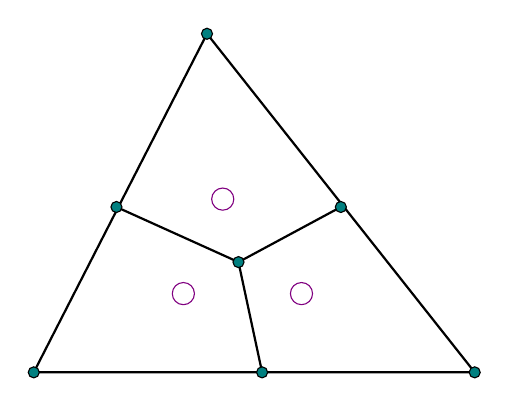
\begin{tikzpicture}
\draw[thick] (0,0) -- (5.6,0) -- (2.2,4.3)-- cycle;  
\draw[thick] (1.05,2.1) -- (2.6,1.4) -- (3.9,2.1);  
\draw[thick] (2.6,1.4) -- (2.9,0);  
\draw[black,fill=teal] (0,0) circle (2pt);
\draw[black,fill=teal] (5.6,0) circle (2pt);
\draw[black,fill=teal] (2.2,4.3) circle (2pt);
\draw[black,fill=teal] (1.05,2.1) circle (2pt);
\draw[black,fill=teal] (2.6,1.4) circle (2pt);
\draw[black,fill=teal] (3.9,2.1) circle (2pt);
\draw[black,fill=teal] (2.9,0) circle (2pt);
\draw[violet] (1.9,1) circle (4pt);
\draw[violet] (3.4,1) circle (4pt);
\draw[violet] (2.4,2.2) circle (4pt);
\end{tikzpicture}
\end{center}


{\color{MidnightBlue}
For simplicity, consider the two-dimensional case. Figure [above] shows how a quadratic
triangular element enriched with a node placed at the barycenter of the triangle can
be splitted into three bilinear elements. If we consider a pressure unknown for each
quadrilateral, we see that the velocity and pressure spaces will be isomorphic to those
of the $P_2^+ \times P_{-1}$ element [...]. The velocity-pressure interpolation for this
element satisfies the BB condition. Therefore, the macroelement depicted in [the figure above]
composed of $Q_1 \times P_0$ elements will also be div-stable.

Clearly, the main problem with this approach is the distorsion of the triangular
patch of three quadrilaterals. This patch has to be regular enough (i.e., the angles
sufficiently close to $\pi/3$) to ensure that the isoparametric mapping to the parent domain
(usually $[-1,1] \times [-1,1]$) be invertible. See Reference \cite{ciarlet2002finite} 
for the regularity conditions that a finite element partition has to satisfy.

The macroelement of [the figure above] is homeomorphic to the macroelement of Le Tallec
\& Ruas \cite{leru86}.
In the three-dimensional case, the $P_2^+ \times P_{-1}$ 
element has to be splitted into four $Q_1 \times P_0$ subelements. 
Apparently, this connexion between the $P_2^+ \times P_{-1}$ and the $Q_1 \times P_0$
elements has never been exploited.}

\end{displayquote}

We indeed find this subdivided triangle m-e in QZ1 and QZ3. 

%...................................................
\paragraph{Location of nodes inside macro element}.
When possible, we wish that all elements of a macro-element have the same area. 
For the Stenberg macro-element, we set $\delta =0.3$ (see remark at the end).
For the Le Tallex macro-element, we set $\delta=h/\sqrt{12}$ (see remark at the end).
We also make sure that all elements in QZ1,QZ3,B have same area.
However, there is a problem with QZ2: equi area yields quads with angle=$180^o$. 
Likewise macro-element T1 cannot be generated with all elements equi-area.


%................................................
\paragraph{Removal of checkerboard pattern via perturbation}

We read in \textcite{lumh24}:
\begin{displayquote}
{\color{MidnightBlue}
Griffiths and Silvester (1994) demonstrates a simple way to remove the checker-board 
error associated with the Q1-P0 element. One only needs to add a small perturbation 
to the coordinates of grid points. Here we adopt this approach in our two-phase 
implementation and perturb the coordinates of the internal vertices by 5\% of the
element size.
}
\end{displayquote}


This does not mean that it is usable with iterative solver?










%---------------------------------
\section*{Implementation}

There are 14 benchmarks/experiments that are currently implemented in the code:
\begin{enumerate}
\item Donea \& Huerta (MS) %1
\item block in the middle %2
\item sphere in the middle %3
\item aquarium %4
\item SolKz (MS) %5
\item regularised lid driven cavity %6
\item cavity (MS) %7
\item sinking block %8
\item Dohrmann \& Bochev (MS) \cite{dobo04} %9
\item flow around square cylinder % 10
\item flow over cavity % 11
\item flow over obstacle %12
\item SolCx (MS) %13
\item SolVi (MS) %14
\end{enumerate}
where MS stands for `manufactured solution'.

All experiments take place in the unit square expect experiment 8.

All experiments are isoviscous expect 3,5,8,13,14.
Note that the viscosity is evaluated in the middle of each element, not 
at the quadrature points. This can/will have an effect on non-isoviscous models.

\newpage
The meshes are created by importing the corresponding files:
\begin{lstlisting} 
import regular
import macro_S
import macro_LT
import macro_QZ1 
import macro_QZ2
import macro_QZ3
import macro_T1
import macro_T2
\end{lstlisting} 
Inside each of these files a function called {\sl mesher} is defined: 
\begin{lstlisting} 
def mesher(Lx,Ly,nelx,nely,nel,NV,mV):
\end{lstlisting} 
The arguments are the domain size $L_x$ and $L_y$, the number of macroelements
in each direction $nelx$ and $nely$, the precomputed total number of $Q_1\times P_0$ 
elements $nel$ and nodes $NV$ and the number of nodes per element $m_\upnu$.  

In what follows $p$ is the 'raw' pressure field (after normalisation)
while $q$ denotes its projection onto the nodes by means of corner-to-node average.
More specifically $q_1$ is the pressure average at the node, 
while $q_2$  is the element area weighed average.
In practice most of the macro-elements are built so that 
the elements inside it have equal area and then $q_1=q_2$. 

Define errors and mesh size which is taken to be $h = \sqrt{L_xL_y/nel}$. 

%------------------------------------
\subsection*{Pressure normalization}

When it comes to the requirement of $\int_\Omega p dV=0$ we have three options
in order to enforce this constraint:
\begin{enumerate}
\item build the matrix without taking care of this constraint, and 
enforce it after the solve:
\[
\int_\Omega p dV = \sum_e A_e p_e = 0
\]
with $A_e$ being the area of element $e$.

\item Add a line and column to the matrix (Lagrange multiplier technique)
and effectively add the vector $(A_0,	 A_1, ... A_{nel-1})$ below and to the 
right of the zero pressure-pressure block of the Stokes matrix. 
The recovered pressure is then such that $sum_e A_e p_e = 0$
and the normalisation loop that comes after is useless (if only to 
verify that indeed $<p>=0$).
Post-solve normalisation is then not needed but acts as a check 
and typically returns zero (within machine precision).

\item add a line and column to the matrix that enforces $p_{nel}=0$
(or any value, really), solve the linear system and then 
normalize the pressure as in Option 1.

\end{enumerate}

Option 1 is the simplest and it works fine, except for 
experiment 9, which has a velocity field that 
does not showcases no-slip b.c.:

\begin{center}
\includegraphics[width=5cm]{python_codes/fieldstone_78/results/exp09/vel.png}
\includegraphics[width=5cm]{python_codes/fieldstone_78/results/exp09/press.png}\\
{\captionfont Experiment 9: velocity and pressure fields.}
\end{center}

I then found out that Option 2 worked {\it much} better for this experiment
and allowed to recover accurate velocities, mild pressure checkerboarding.
However the addition of the extra line probably\footnote{I cannot check this 
for sure but it makes sense -- more on this later} generated a lot of fill-ins in the direct solver
and slowed things down considerably.

\begin{center}
\includegraphics[width=5cm]{python_codes/fieldstone_78/images/lagrange/A_bef.png}\\
{\captionfont Example of $20\times 20$ QZ2 macro-element matrix sparsity pattern.}
\end{center}

we can verify that the three options result in the same results 
for experiment 1 for example:

{\small
\begin{verbatim}
*****Option 1*****
nel=   2400 ; errv= 0.00003035857 ; errp= 0.00419435407 ; errq1= 0.00153250868 
solve time: 0.132 s
*****Option 2*****
nel=   2400 ; errv= 0.00003035857 ; errp= 0.00419435407 ; errq1= 0.00153250868 
solve time: 1.314 s
*****Option 3*****
nel=   2400 ; errv= 0.00003035857 ; errp= 0.00419435407 ; errq1= 0.00153250868 
solve time: 0.130 s
\end{verbatim}
}

We see that Option 2 is definitely *much* slower than option 3!
and when carrying out resolution tests I found that Option 2 slowed 
the solver so much that it became unpractical. 
Also I found out that Option 2 worked but Option 3 did not (again, for experiment 9), which makes little sense. 
I then decided to follow and other lead and started to think again about the fact that 
experiment 9 showcases a non-zero flux on various faces. 

I then *suspected* that this behavior could be due to the fact 
may be there is some kind of imbalance in the overal (discrete)
flux (flow is incompressible, we should have $\int_\Gamma \vec{u}\cdot\vec{n} \; dS=0$) 
and therefore triggers extremely large insane pressure oscillations and 
yields the problem above? my instinct then tells me that 
by adding this extra line (and corresponding column) of constraints in the matrix it somewhat 
introduces some 'wiggle room' (\#technicalterm:) that compensates for the error in the b.c. imposition?
However, since option 2 is not an option in reality, what to do? 
 
For once we could start by computing the analytical flux on each face for experiment 9:
\begin{eqnarray}
\Phi_{bottom} 
&=& \int_0^1 \vec{\upnu}(x,y=0) \cdot \vec{n} \; dx \nn\\
&=& -\int_0^1 v(x,y=0)  dx \nn\\
&=& 0 \nn\\
\Phi_{top} 
&=& \int_0^1 \vec{\upnu}(x,y=1) \cdot \vec{n} \; dx \nn\\
&=& \int_0^1 v(x,y=1)  dx \nn\\
&=& \int_0^1 ( -1-2x+1 -3x^2 + 1 - x ) dx \nn\\
&=& \int_0^1 ( -3x+1 -3x^2   ) dx \nn\\
&=& -3/2 \nn\\
\Phi_{left} 
&=& \int_0^1 \vec{\upnu}(x=0,y) \cdot \vec{n} \; dy \nn\\
&=& -\int_0^1 u(x=0,y)  dy \nn\\
&=& 0 \nn\\
\Phi_{right} 
&=& \int_0^1 \vec{\upnu}(x=1,y) \cdot \vec{n} \; dy \nn\\
&=& \int_0^1 u(x=1,y)  dy \nn\\
&=& \int_0^1 (3  - y - 3y^2  ) dy \nn\\
&=& 3/2 \nn
\end{eqnarray}
And of course we find 
\[
\Phi_{total}=\Phi_{bottom}+\Phi_{top} +\Phi_{left}  + \Phi_{right}  =0
\] 
We expected this since
\[
\int_\Omega \vec{\nabla}\cdot \vec{\upnu} \; dV 
= \int_\Gamma \vec{\upnu} \cdot \vec{n} \; dS
=\Phi_{total}=\Phi_{bottom}+\Phi_{top} +\Phi_{left}  + \Phi_{right}  =0
\]

Now turning to measurements of these fluxes on each boundary,
we compute these by means of a one point quadrature on each 
element edge that is on a boundary.
The algorithm goes as follows for one of the four fluxes:
\begin{lstlisting}
flux_bottom=0
for iel in range(0,nel):
    inode0=iconV[0,iel]
    inode1=iconV[1,iel]
    inode2=iconV[2,iel]
    inode3=iconV[3,iel]
    if abs(yV[inode0]-0)/Ly<eps and abs(yV[inode1]-0)/Ly<eps:
       flux_bottom+=abs(xV[inode0]-xV[inode1])*(bc_val[inode0*ndofV+1]+bc_val[inode1*ndofV+1])/2 *-1
    if abs(yV[inode1]-0)/Ly<eps and abs(yV[inode2]-0)/Ly<eps:
       flux_bottom+=abs(xV[inode1]-xV[inode2])*(bc_val[inode1*ndofV+1]+bc_val[inode2*ndofV+1])/2 *-1
    if abs(yV[inode2]-0)/Ly<eps and abs(yV[inode3]-0)/Ly<eps:
       flux_bottom+=abs(xV[inode2]-xV[inode3])*(bc_val[inode2*ndofV+1]+bc_val[inode3*ndofV+1])/2 *-1
    if abs(yV[inode3]-0)/Ly<eps and abs(yV[inode0]-0)/Ly<eps:
       flux_bottom+=abs(xV[inode3]-xV[inode0])*(bc_val[inode3*ndofV+1]+bc_val[inode0*ndofV+1])/2 *-1
\end{lstlisting}
 
For a $32\times 32$ (R) mesh we find:
\begin{verbatim}
flux b,t,l,r= 0.0 -1.5001220703125 0.0 1.4998779296875
total_flux= -0.000244140625
\end{verbatim}
We see that the total flux is not zero (at least down to machine precision)
and this is likely to introduce a problem.

I then prescribe on the nodes of the boundary the following velocity:
\[
\vec{\upnu}^{bc} = \vec{\upnu}_{analytical} - \frac{\Phi_{measured}}{P} \vec{n}
\]
where $\Phi_{measured}$ is the measured velocity flux 
through the entire boundary and $P$ is the perimeter of the domain.
Then 
\begin{eqnarray}
\int_\Gamma \vec{\upnu}^{bc} \cdot \vec{n} \; dS
&=& \int_\Gamma \vec{\upnu}_{analytical} \cdot \vec{n} \; dS
- \int_\Gamma  \frac{\Phi_{measured}}{P} \vec{n} \cdot \vec{n} \; dS\nn\\
&=& \Phi_{measured} - \frac{\Phi_{measured}}{P} \int_\Gamma  1 \; dS \nn\\
&=& \Phi_{measured} - \frac{\Phi_{measured}}{P} P \nn\\
&=&0 \nn
\end{eqnarray}
assuming that the normal vector is a unit vector, i.e. $\vec{n}\cdot \vec{n}=1$.
I then find that applying this correction does solve the problem 
and that Option 1 is now usable again for all topologies.

Note that the problem of the normal vector at the corners does not
present itself: the quadrature points are in the middle 
of element edges and the normal vector is well defined there.

This velocity correction is transparent to all 
manufactured solutions or experiments that 
showcase free-slip or no-slip boundary conditions.

This is controled by the {\tt correct\_bcval} parameter. 

Remark: see page 291 of \textcite{vibo92} (1992).

%--------------------------------------------------------------
\subsection*{About reordering ...}

While exploring the pressure normalisation I observed that 
Option 2 was much slower than the others. I attributed this 
to the number of fill-ins generated because of the full line
added at the bottom of the pressure-pressure block. 

I then proceeded to look into reordering the complete 
Stokes matrix via the Reverse Cuthill-McKee 
algorithm\footnote{\url{https://en.wikipedia.org/wiki/Cuthill-McKee_algorithm}}
(see also \ref{MMS-ss:reordering}) which is available via SciPy:
\begin{lstlisting} 
from scipy.sparse.csgraph import reverse_cuthill_mckee
\end{lstlisting} 
Once the matrix is fully assembled I use the 'spy' function 
to generate a plot of its sparsity patten.
I then proceed to use the RCM algorithm as follows:
\begin{lstlisting} 
if apply_RCM:
   perm=reverse_cuthill_mckee(A_csr,symmetric_mode=True)
   perm_inv=np.empty(len(perm),dtype=np.int32)
   for i in range(0,len(perm)):
       perm_inv[perm[i]]=i
   A_csr=A_csr[np.ix_(perm,perm)]
   rhs=rhs[np.ix_(perm)]
\end{lstlisting} 
Another snapshot of the matrix is then produced after the reordering. 
Before and after snapshots are shown below for all 8 topologies 
(in the absence of any pressure normalisation Lagrange multiplier line):

\begin{center}
\includegraphics[width=4cm]{python_codes/fieldstone_78/results/spy/A_bef_topo0.pdf}
\includegraphics[width=4cm]{python_codes/fieldstone_78/results/spy/A_bef_topo1.pdf}
\includegraphics[width=4cm]{python_codes/fieldstone_78/results/spy/A_bef_topo2.pdf}
\includegraphics[width=4cm]{python_codes/fieldstone_78/results/spy/A_bef_topo3.pdf}\\
\includegraphics[width=4cm]{python_codes/fieldstone_78/results/spy/A_bef_topo4.pdf}
\includegraphics[width=4cm]{python_codes/fieldstone_78/results/spy/A_bef_topo5.pdf}
\includegraphics[width=4cm]{python_codes/fieldstone_78/results/spy/A_bef_topo6.pdf}
\includegraphics[width=4cm]{python_codes/fieldstone_78/results/spy/A_bef_topo7.pdf}\\
{\captionfont Before: 4x4 macro-element mesh}
\end{center}

\begin{center}
\includegraphics[width=4cm]{python_codes/fieldstone_78/results/spy/A_aft_topo0.pdf}
\includegraphics[width=4cm]{python_codes/fieldstone_78/results/spy/A_aft_topo1.pdf}
\includegraphics[width=4cm]{python_codes/fieldstone_78/results/spy/A_aft_topo2.pdf}
\includegraphics[width=4cm]{python_codes/fieldstone_78/results/spy/A_aft_topo3.pdf}\\
\includegraphics[width=4cm]{python_codes/fieldstone_78/results/spy/A_aft_topo4.pdf}
\includegraphics[width=4cm]{python_codes/fieldstone_78/results/spy/A_aft_topo5.pdf}
\includegraphics[width=4cm]{python_codes/fieldstone_78/results/spy/A_aft_topo6.pdf}
\includegraphics[width=4cm]{python_codes/fieldstone_78/results/spy/A_aft_topo7.pdf}\\
{\captionfont After: 4x4 macro-element mesh}
\end{center}

After the solve, the solution vector must be reordered to 
comply with the connectivity array:
\begin{lstlisting} 
if apply_RCM:
   sol=sol[np.ix_(perm_inv)]
\end{lstlisting} 















\newpage
%-----------------------------------------------------------------
\subsection*{Testing for the existence of checkerboard modes}



\[
\G_{el} = -\int_{\Omega_e} {\bm B}^T \cdot {\bm N} dV
= -\int_{\Omega_e}
\left(
\begin{array}{ccc}
\partial_x \bN_1^\upnu & 0 & \partial_y \bN_1^\upnu \\
0 & \partial_y \bN_1^\upnu & \partial_x \bN_1^\upnu \\
\partial_x \bN_2^\upnu & 0 & \partial_y \bN_2^\upnu \\
0 & \partial_y \bN_2^\upnu & \partial_x \bN_2^\upnu \\
\dots & \dots & \dots \\
\dots & \dots & \dots \\
\partial_x \bN_{m_\upnu}^\upnu & 0 & \partial_y \bN_{m_\upnu}^\upnu \\
0 & \partial_y \bN_{m_\upnu}^\upnu & \partial_x \bN_{m_\upnu}^\upnu 
\end{array}
\right)
\cdot
\left(
\begin{array}{cccc}
\bN_1^p & \bN_2^p & \dots & \bN_{m_p}^p \\ 
\bN_1^p & \bN_2^p & \dots & \bN_{m_p}^p \\ 
0 & 0 & \dots & 0
\end{array}
\right)
dV
\]
Since we are dealing with $Q_1\times P_0$ elements then $m_p=1$ and $\bN^p(x,y)=1$.
This yields
\[
\G_{el} = -\int_{\Omega_e} {\bm B}^T \cdot {\bm N} dV
= -\int_{\Omega_e}
\left(
\begin{array}{ccc}
\partial_x \bN_1^\upnu \\
\partial_y \bN_1^\upnu \\
\partial_x \bN_2^\upnu \\
\partial_y \bN_2^\upnu \\
\partial_x \bN_3^\upnu \\
\partial_y \bN_3^\upnu \\
\partial_x \bN_4^\upnu \\
\partial_y \bN_4^\upnu 
\end{array}
\right)
dV
\]

In what follows we proceed to build the assembled block $\G$ for each macro element, 
impose no slip boundary conditions on all sides (thereby zeroing many lines of the
matrix), and compute the null space of the remaining lines. 
Ideally only one pressure solution should be in the null space, the space of 
all constant vectors since then $\G \cdot \vec{\cal P}=\vec{0}$.
If/when the nullspace is larger than one, then checkerboard patterns (aka 
spurious modes) can exist and degrade the solution. 

This study can be carried out by setting the \lstinline{nullspace} parameter to 
\lstinline{True} and the number of elements and domain size is then set automatically.

\newpage
The 8 macro-elements considered here are shown hereunder 
with their internal numbering of nodes:

\begin{center}
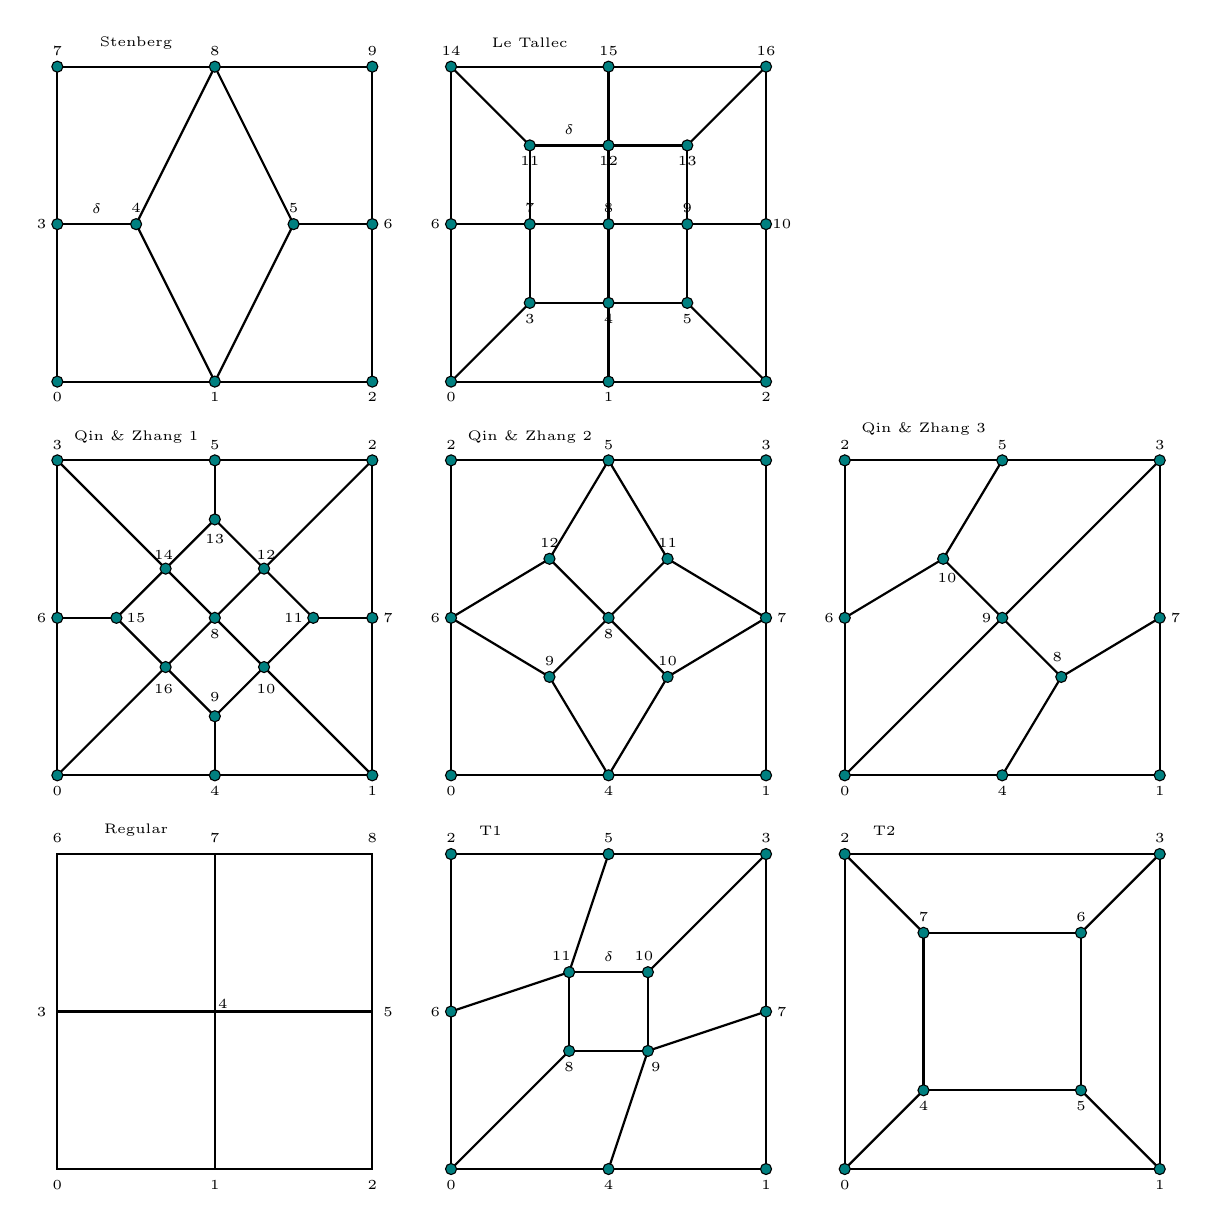
\begin{tikzpicture}
%\draw[fill=gray!23,gray!23](0,0) rectangle (15,15);
%\draw[step=0.5cm,gray,very thin] (0,0) grid (15,15); %background grid


%%%%%%%%%%%%%%%%%%%%%%%%%%%%%%%%%%%%%%%%%%%%%%%%%%%%%%%%%%%%%%%%%%
%stenberg
\node[] at (1,14.3) {\tiny Stenberg};
\draw[thick] (0,10) -- (4,10) -- (4,14) -- (0,14) -- cycle;  
\draw[thick] (2,10) -- (3,12) -- (2,14) -- (1,12) -- cycle;  
\draw[thick] (0,12) -- (1,12);  
\draw[thick] (3,12) -- (4,12);  
\draw[black,fill=teal] (0,10) circle (2pt);
\draw[black,fill=teal] (4,10) circle (2pt);
\draw[black,fill=teal] (4,14) circle (2pt);
\draw[black,fill=teal] (0,14) circle (2pt);
\draw[black,fill=teal] (2,10) circle (2pt);
\draw[black,fill=teal] (2,14) circle (2pt);
\draw[black,fill=teal] (0,12) circle (2pt);
\draw[black,fill=teal] (4,12) circle (2pt);
\draw[black,fill=teal] (1,12) circle (2pt);
\draw[black,fill=teal] (3,12) circle (2pt);

\node[] at (0,10-0.2) {\tiny 0};
\node[] at (4,10-0.2) {\tiny 2};
\node[] at (4,14+0.2) {\tiny 9};
\node[] at (0,14+0.2) {\tiny 7};
\node[] at (2,10-0.2) {\tiny 1};
\node[] at (2,14+0.2) {\tiny 8};
\node[] at (0-0.2,12) {\tiny 3};
\node[] at (4+0.2,12) {\tiny 6};
\node[] at (1,12+0.2) {\tiny 4};
\node[] at (3,12+0.2) {\tiny 5};


\node[] at (0.5,12.2) {\tiny $\delta$};

%%%%%%%%%%%%%%%%%%%%%%%%%%%%%%%%%%%%%%%%%%%%%%%%%%%%%%%%%%%%%%%%%%%
%letallec
\node[] at (6,14.3) {\tiny Le Tallec};
\draw[thick] (5,10) -- (9,10) -- (9,14) -- (5,14) -- cycle;  
\draw[thick] (6,11) -- (8,11) -- (8,13) -- (6,13) -- cycle;  
\draw[thick] (5,10) -- (6,11) ;  
\draw[thick] (9,10) -- (8,11) ;  
\draw[thick] (9,14) -- (8,13) ;  
\draw[thick] (5,14) -- (6,13) ;  
\draw[thick] (5,12) -- (9,12) ;  
\draw[thick] (7,10) -- (7,14) ;  
\draw[black,fill=teal] (0+5,10) circle (2pt);
\draw[black,fill=teal] (4+5,10) circle (2pt);
\draw[black,fill=teal] (4+5,14) circle (2pt);
\draw[black,fill=teal] (0+5,14) circle (2pt);
\draw[black,fill=teal] (6,11) circle (2pt);
\draw[black,fill=teal] (8,11) circle (2pt);
\draw[black,fill=teal] (8,13) circle (2pt);
\draw[black,fill=teal] (6,13) circle (2pt);
\draw[black,fill=teal] (7,10) circle (2pt);
\draw[black,fill=teal] (5,12) circle (2pt);
\draw[black,fill=teal] (9,12) circle (2pt);
\draw[black,fill=teal] (7,14) circle (2pt);
\draw[black,fill=teal] (6,12) circle (2pt);
\draw[black,fill=teal] (7,12) circle (2pt);
\draw[black,fill=teal] (8,12) circle (2pt);
\draw[black,fill=teal] (7,11) circle (2pt);
\draw[black,fill=teal] (7,13) circle (2pt);


\node[] at (0+5,10-0.2) {\tiny 0};
\node[] at (2+5,10-0.2) {\tiny 1};
\node[] at (4+5,10-0.2) {\tiny 2};
\node[] at (1+5,11-0.2) {\tiny 3};
\node[] at (2+5,11-0.2) {\tiny 4};
\node[] at (3+5,11-0.2) {\tiny 5};
\node[] at (0-0.2+5,12) {\tiny 6};
\node[] at (1+5,12+0.2) {\tiny 7};
\node[] at (2+5,12+0.2) {\tiny 8};
\node[] at (3+5,12+0.2) {\tiny 9};
\node[] at (4+0.2+5,12) {\tiny 10};
\node[] at (1+5,13-0.2) {\tiny 11};
\node[] at (2+5,13-0.2) {\tiny 12};
\node[] at (3+5,13-0.2) {\tiny 13};
\node[] at (0+5,14+0.2) {\tiny 14};
\node[] at (2+5,14+0.2) {\tiny 15};
\node[] at (4+5,14+0.2) {\tiny 16};

\node[] at (6.5,13.2) {\tiny $\delta$};

%%%%%%%%%%%%%%%%%%%%%%%%%%%%%%%%%%%%%%%%%%%%%%%%%%%%%%%%%%%%%%%%%%
%qizh1
\node[] at (1,9.3) {\tiny Qin \& Zhang 1};

\draw[thick] (0,5) -- (4,5) -- (4,9) -- (0,9) -- cycle;  
\draw[thick] (1.75-1,3+4) -- (3-1,1.75+4) -- (4.25-1,3+4) -- (3-1,4.25+4) -- cycle;  
\draw[thick] (1-1,1+4) -- (5-1,5+4) ;  
\draw[thick] (1-1,5+4) -- (5-1,1+4) ;  
\draw[thick] (3-1,1+4) -- (3-1,1.75+4) ;  
\draw[thick] (3-1,4.25+4) -- (3-1,5+4) ;  
\draw[thick] (1-1,3+4) -- (1.75-1,3+4) ;  
\draw[thick] (4.25-1,3+4) -- (5-1,3+4) ;  
\draw[black,fill=teal] (1-1,1+4)   circle (2pt);
\draw[black,fill=teal] (3-1,1+4)   circle (2pt);
\draw[black,fill=teal] (5-1,1+4)   circle (2pt);

\draw[black,fill=teal] (3-1,1.75+4)   circle (2pt);
\draw[black,fill=teal] (2.375-1,2.375+4)   circle (2pt);
\draw[black,fill=teal] (3.625-1,2.375+4)   circle (2pt);

\draw[black,fill=teal] (1-1,3+4)   circle (2pt);
\draw[black,fill=teal] (1.75-1,3+4)   circle (2pt);
\draw[black,fill=teal] (3-1,3+4)   circle (2pt);
\draw[black,fill=teal] (4.25-1,3+4)   circle (2pt);
\draw[black,fill=teal] (5-1,3+4)   circle (2pt);

\draw[black,fill=teal] (2.375-1,3.625+4)   circle (2pt);
\draw[black,fill=teal] (3.625-1,3.625+4)   circle (2pt);
\draw[black,fill=teal] (3-1,4.25+4)   circle (2pt);

\draw[black,fill=teal] (1-1,5+4)   circle (2pt);
\draw[black,fill=teal] (3-1,5+4)   circle (2pt);
\draw[black,fill=teal] (5-1,5+4)   circle (2pt);


\node[] at (0,5-0.2) {\tiny 0};
\node[] at (2,5-0.2) {\tiny 4};
\node[] at (4,5-0.2) {\tiny 1};
\node[] at (0-0.2,7) {\tiny 6};
\node[] at (1,7) {\tiny 15};
\node[] at (2,7-0.2) {\tiny 8};
\node[] at (3,7) {\tiny 11};
\node[] at (4+0.2,7) {\tiny 7};
\node[] at (2,6) {\tiny 9};
\node[] at (2,8) {\tiny 13};
\node[] at (0,9+0.2) {\tiny 3};
\node[] at (2,9+0.2) {\tiny 5};
\node[] at (4,9+0.2) {\tiny 2};

\node[] at (1.35,6.1) {\tiny 16};
\node[] at (2.65,6.1) {\tiny 10};
\node[] at (1.35,7.8) {\tiny 14};
\node[] at (2.65,7.8) {\tiny 12};



%%%%%%%%%%%%%%%%%%%%%%%%%%%%%%%%%%%%%%%%%%%%%%%%%%%%%%%%%%%%%
\draw[thick] (5,5) -- (9,5) -- (9,9) -- (5,9) -- cycle;  
\node[] at (6,9.3) {\tiny Qin \& Zhang 2};

\draw[thick] (1+4,3+4) -- (2.25+4,2.25+4) -- (3+4,1+4) -- (3.75+4,2.25+4) -- (5+4,3+4) --(3.75+4,3.75+4) -- (3+4,5+4) --(2.25+4,3.75+4) --cycle;  
\draw[thick] (2.25+4,2.25+4) -- (3.75+4,3.75+4) ;  %diags
\draw[thick] (2.25+4,3.75+4) -- (3.75+4,2.25+4) ;  

\draw[black,fill=teal] (1+4,1+4)   circle (2pt); %perimeter nodes
\draw[black,fill=teal] (3+4,1+4)   circle (2pt);
\draw[black,fill=teal] (5+4,1+4)   circle (2pt);
\draw[black,fill=teal] (1+4,3+4)   circle (2pt);
\draw[black,fill=teal] (3+4,3+4)   circle (2pt);
\draw[black,fill=teal] (5+4,3+4)   circle (2pt);
\draw[black,fill=teal] (1+4,5+4)   circle (2pt);
\draw[black,fill=teal] (3+4,5+4)   circle (2pt);
\draw[black,fill=teal] (5+4,5+4)   circle (2pt);

\draw[black,fill=teal] (2.25+4,2.25+4)   circle (2pt); %inside nodes
\draw[black,fill=teal] (3.75+4,3.75+4)   circle (2pt);
\draw[black,fill=teal] (2.25+4,3.75+4)   circle (2pt);
\draw[black,fill=teal] (3.75+4,2.25+4)   circle (2pt);


\node[] at (1+4,1+4-0.2) {\tiny 0};
\node[] at (1+6,1+4-0.2) {\tiny 4};
\node[] at (1+8,1+4-0.2) {\tiny 1};
\node[] at (1+4-0.2,1+6) {\tiny 6};
\node[] at (1+6,1+6-0.2) {\tiny 8};
\node[] at (1+8+0.2,1+6) {\tiny 7};
\node[] at (1+4,1+8+0.2) {\tiny 2};
\node[] at (1+6,1+8+0.2) {\tiny 5};
\node[] at (1+8,1+8+0.2) {\tiny 3};
\node[] at (2.25+4,2.25+4+0.2) {\tiny 9};
\node[] at (2.25+4+1.5,2.25+4+0.2) {\tiny 10};
\node[] at (2.25+4,2.25+4+1.5+0.2) {\tiny 12};
\node[] at (2.25+4+1.5,2.25+4+1.5+0.2) {\tiny 11};


%%%%%%%%%%%%%%%%%%%%%%%%%%%%%%%%%%%%%%%%%%%%%%%%%%%%%%%%%%%%%
\node[] at (11,9.4) {\tiny Qin \& Zhang 3};
\draw[thick] (10,5) -- (14,5) -- (14,9) -- (10,9) -- cycle;  

\draw[thick] (1+9,3+4) -- (2.25+9,3.75+4) -- (3+9,5+4);
\draw[thick] (3+9,1+4) -- (3.75+9,2.25+4) -- (5+9,3+4);
\draw[thick] (1+9,1+4) -- (5+9,5+4) ;  %diags
\draw[thick] (2.25+9,3.75+4) -- (3.75+9,2.25+4) ;  

\draw[black,fill=teal] (1+9,1+4)   circle (2pt); %perimeter nodes
\draw[black,fill=teal] (3+9,1+4)   circle (2pt);
\draw[black,fill=teal] (5+9,1+4)   circle (2pt);
\draw[black,fill=teal] (1+9,3+4)   circle (2pt);
\draw[black,fill=teal] (3+9,3+4)   circle (2pt);
\draw[black,fill=teal] (5+9,3+4)   circle (2pt);
\draw[black,fill=teal] (1+9,5+4)   circle (2pt);
\draw[black,fill=teal] (3+9,5+4)   circle (2pt);
\draw[black,fill=teal] (5+9,5+4)   circle (2pt);
\draw[black,fill=teal] (2.25+9,3.75+4)   circle (2pt); %inside nodes
\draw[black,fill=teal] (3.75+9,2.25+4)   circle (2pt);


\node[] at (1+9,1+4-0.2) {\tiny 0};
\node[] at (3+9,1+4-0.2) {\tiny 4};
\node[] at (5+9,1+4-0.2) {\tiny 1};

\node[] at (1+9-0.2,1+6) {\tiny 6};
\node[] at (1+9+4+0.2,1+6) {\tiny 7};
\node[] at (1+9+2.5+0.2,1+5.5) {\tiny 8};
\node[] at (1+9+2-0.2,1+6) {\tiny 9};
\node[] at (1+9+1.5-0.2,1+6.5) {\tiny 10};

\node[] at (1+9,1+8+0.2) {\tiny 2};
\node[] at (3+9,1+8+0.2) {\tiny 5};
\node[] at (5+9,1+8+0.2) {\tiny 3};



%%%%%%%%%%%%%%%%%%%%%%%%%%%%%%%%%%%%%%%%%%%%%%%%%%%%%%%%%%%%%
%mineB
\node[] at (0.5+10,4.3) {\tiny T2};
\draw[thick] (0+10,0) -- (4+10,0) -- (4+10,4) -- (0+10,4) -- cycle;  
\draw[thick] (1+10,1) -- (3+10,1) -- (3+10,3) -- (1+10,3) -- cycle;  
\draw[thick] (0+10,0) -- (1+10,1);  
\draw[thick] (4+10,0) -- (3+10,1); 
\draw[thick] (4+10,4) -- (3+10,3);  
\draw[thick] (0+10,4) -- (1+10,3);  
\draw[black,fill=teal] (0+10,0)   circle (2pt);
\draw[black,fill=teal] (4+10,0)   circle (2pt);
\draw[black,fill=teal] (4+10,4)   circle (2pt);
\draw[black,fill=teal] (0+10,4)   circle (2pt);
\draw[black,fill=teal] (1+10,1)   circle (2pt);
\draw[black,fill=teal] (3+10,1)   circle (2pt);
\draw[black,fill=teal] (3+10,3)   circle (2pt);
\draw[black,fill=teal] (1+10,3)   circle (2pt);

\node[] at (0+10,0-0.2) {\tiny 0};
\node[] at (4+10,0-0.2) {\tiny 1};
\node[] at (4+10,4+0.2) {\tiny 3};
\node[] at (0+10,4+0.2) {\tiny 2};
\node[] at (1+10,1-0.2) {\tiny 4};
\node[] at (3+10,1-0.2) {\tiny 5};
\node[] at (1+10,3+0.2) {\tiny 7};
\node[] at (3+10,3+0.2) {\tiny 6};


%%%%%%%%%%%%%%%%%%%%%%%%%%%%%%%%%%%%%%%%%%%%%%%%%%%%%%%%%%%%%
%mineA
\node[] at (5.5,4.3) {\tiny T1};
\draw[thick] (5,0) -- (9,0) -- (9,4) -- (5,4) -- cycle;  
\draw[thick] (6.5,1.5) -- (7.5,1.5) -- (7.5,2.5) -- (6.5,2.5) -- cycle;  

\draw[thick] (5,0) --(6.5,1.5);
\draw[thick] (7,0) --(7.5,1.5)--(9,2);
\draw[thick] (5,2) --(6.5,2.5)--(7,4);
\draw[thick] (7.5,2.5) --(9,4);

\draw[black,fill=teal] (5,0)   circle (2pt);
\draw[black,fill=teal] (9,0)   circle (2pt);
\draw[black,fill=teal] (9,4)   circle (2pt);
\draw[black,fill=teal] (5,4)   circle (2pt);
\draw[black,fill=teal] (6.5,1.5)   circle (2pt);
\draw[black,fill=teal] (7.5,1.5)   circle (2pt);
\draw[black,fill=teal] (7.5,2.5)   circle (2pt);
\draw[black,fill=teal] (6.5,2.5)   circle (2pt);

\draw[black,fill=teal] (7,0)   circle (2pt);
\draw[black,fill=teal] (7,4)   circle (2pt);
\draw[black,fill=teal] (5,2)   circle (2pt);
\draw[black,fill=teal] (9,2)   circle (2pt);

\node[] at (7,2.7) {\tiny $\delta$};

\node[] at (5,0-0.2) {\tiny 0};
\node[] at (5-0.2,2) {\tiny 6};
\node[] at (9+0.2,2) {\tiny 7};

\node[] at (5+2,0-0.2) {\tiny 4};
\node[] at (5+4,0-0.2) {\tiny 1};
\node[] at (5,4+0.2) {\tiny 2};
\node[] at (5+2,4+0.2) {\tiny 5};
\node[] at (5+4,4+0.2) {\tiny 3};

\node[] at (5+1.5,1.5-0.2) {\tiny 8};
\node[] at (5+2.6,1.5-0.2) {\tiny 9};
\node[] at (5+1.4,2.5+0.2) {\tiny 11};
\node[] at (5+2.45,2.5+0.2) {\tiny 10};

%%%%%%%%%%%%%%%%%%%%%%%%%%%%%%%%%%%%%%%%%%%%%%%%%%%%%%%%%%%%%
%regular

\node[] at (1,4.3) {\tiny Regular};

\draw[thick] (0,0) -- (4,0) -- (4,4) -- (0,4) -- cycle;  
\draw[thick] (0,2) -- (4,2) ;  
\draw[thick] (2,0) -- (2,4) ;  

\node[] at (0,0-0.2) {\tiny 0};
\node[] at (2,0-0.2) {\tiny 1};
\node[] at (4,0-0.2) {\tiny 2};

\node[] at (0-0.2,2) {\tiny 3};
\node[] at (2.1,2.1) {\tiny 4};
\node[] at (4+0.2,2) {\tiny 5};

\node[] at (0,4+0.2) {\tiny 6};
\node[] at (2,4+0.2) {\tiny 7};
\node[] at (4,4+0.2) {\tiny 8};

\end{tikzpicture}
\end{center}

Let us consider the regular macro-element consisting of an array of $2\times 2$ rectangular elements. 
The assembled $\G$ matrix is of size $(ndofV \cdot NV, NP)=(NfemV,NfemP)=(18,4)$ and is 
{\small
\begin{verbatim}
0 | [0. 0. 0. 0.]
1 | [0. 0. 0. 0.]
2 | [0. 0. 0. 0.]
3 | [0. 0. 0. 0.]
4 | [0. 0. 0. 0.]
5 | [0. 0. 0. 0.]
6 | [0. 0. 0. 0.]
7 | [0. 0. 0. 0.]
8 | [-0.25  0.25 -0.25  0.25]
9 | [-0.25 -0.25  0.25  0.25]
10 | [0. 0. 0. 0.]
11 | [0. 0. 0. 0.]
12 | [0. 0. 0. 0.]
13 | [0. 0. 0. 0.]
14 | [0. 0. 0. 0.]
15 | [0. 0. 0. 0.]
16 | [0. 0. 0. 0.]
17 | [0. 0. 0. 0.]
\end{verbatim}
}
Indeed, because of boundary conditions on nodes 0,1,2,3,5,6,7,8 all lines 
but the ones corresponding to node 4 (so lines 2*4+0 and 2*4+1) are zeroed. 
We then extract these, which yields the $\tilde{\G}$ matrix:
\[
\tilde{\G}=
\frac14
\begin{pmatrix}
-1 &1 &-1 &1 \\
-1 &-1& 1 &1
\end{pmatrix}
\]
Using the built function \lstinline{null_space} from \lstinline{scipy}, 
\begin{lstlisting}
ns=null_space(G2)
print('null space:')
print(ns)
\end{lstlisting}
we then obtain 
\begin{verbatim}
null space:
[[-0.1  0.7]
 [ 0.7  0.1]
 [ 0.7  0.1]
 [-0.1  0.7]]
\end{verbatim}
If we normalise these vectors so that $<p>=0$ then these two 
pressure vectors are then
\[
\vec{\cal P}=(-0.4,0.4,0.4,-0.4)
\qquad \text{and} \qquad 
\vec{\cal P}=(0.3,-0.3,-0.3,0.3)
\]
which correspong to the following two checker board pressure modes:

{\color{red} DRAW!}


If we now turn to the Stenberg macro-element, the $\G$ matrix 
is of size  $20\times 5$: 
{\small
\begin{verbatim}
0 | [0. 0. 0. 0. 0.]
1 | [0. 0. 0. 0. 0.]
2 | [0. 0. 0. 0. 0.]
3 | [0. 0. 0. 0. 0.]
4 | [0. 0. 0. 0. 0.]
5 | [0. 0. 0. 0. 0.]
6 | [0. 0. 0. 0. 0.]
7 | [0. 0. 0. 0. 0.]
8 | [-0.25  0.    0.5  -0.25  0.  ]
9 | [-0.25  0.    0.    0.25  0.  ]
10 | [ 0.    0.25 -0.5   0.    0.25]
11 | [ 0.   -0.25  0.    0.    0.25]
12 | [0. 0. 0. 0. 0.]
13 | [0. 0. 0. 0. 0.]
14 | [0. 0. 0. 0. 0.]
15 | [0. 0. 0. 0. 0.]
16 | [0. 0. 0. 0. 0.]
17 | [0. 0. 0. 0. 0.]
18 | [0. 0. 0. 0. 0.]
19 | [0. 0. 0. 0. 0.]
\end{verbatim}
}
Again, only the lines corresponding to nodes 4 and 5 are not zeroed.
\[
\tilde{\G}=
\frac14
\begin{pmatrix}
-1 & 0 & 2 &-1 &0 \\
-1 & 0 & 0 & 1 &0 \\
 0 & 1 &-2 & 0 &1 \\
 0 &-1 & 0 & 0 &1
\end{pmatrix}
\]
We finally obtain
\begin{verbatim}
null space:
[[0.4472136]
 [0.4472136]
 [0.4472136]
 [0.4472136]
 [0.4472136]]
\end{verbatim}
The nullspace of $\tilde{\G}$ consists of a single pressure solution, 
the desired constant pressure vector. 

The same is true for all other macro-element of the figure above. 

{\color{red} redo with 2x2 macro-elements !! show T2 is not stable}





\newpage
%-----------------------------------------------------------------
\subsection*{Experiment 1: Donea \& Huerta (MS)}

We start with the Donea \& Huerta manufactured solution (see Section~\ref{MMM-mms1}) and 
proceed to compute the velocity and pressure error convergence as a function of the 
average element size.
we see that the errors converge as expected, quadratically for the velocity and linearly for the pressure.
Rather interestingly the projection of the pressure onto the nodes has a convergence rate 
higher than the raw elemental pressure. As predicted in Qin \& Zhang, the Stenberg macro-element 
yields the best results, followed by the Le Tallec and then the one they propose (this conclusion 
is logically supported by looking at root mean square velocity measurements). 
Finally, the presence of the checkerboard for the regular structure mesh case
makes it painfully clear that it is the worst mesh topology 
and the pressure error does not converge.  

\begin{center}
\includegraphics[width=5cm]{python_codes/fieldstone_78/results/errors_u_exp1.pdf}
\includegraphics[width=5cm]{python_codes/fieldstone_78/results/vrms_exp1.pdf} \\
\includegraphics[width=5cm]{python_codes/fieldstone_78/results/errors_p_exp1.pdf}
\includegraphics[width=5cm]{python_codes/fieldstone_78/results/errors_q1_exp1.pdf}
\includegraphics[width=5cm]{python_codes/fieldstone_78/results/errors_q2_exp1.pdf}\\
\includegraphics[width=5cm]{python_codes/fieldstone_78/results/stats_u_exp1.pdf}
\includegraphics[width=5cm]{python_codes/fieldstone_78/results/stats_v_exp1.pdf}\\
\includegraphics[width=5cm]{python_codes/fieldstone_78/results/stats_p_exp1.pdf}
\includegraphics[width=5cm]{python_codes/fieldstone_78/results/stats_q1_exp1.pdf}
\includegraphics[width=5cm]{python_codes/fieldstone_78/results/stats_q2_exp1.pdf}
\end{center}

On the following figures the pressure is plotted against the analytical solution and 
we see that there is no checkerboarding occurring:
Rather interestingly the pressure error is the largest next to the boundaries.

\begin{center}
0)\includegraphics[width=4cm]{python_codes/fieldstone_78/results/exp01/16x16/p0}
1)\includegraphics[width=4cm]{python_codes/fieldstone_78/results/exp01/16x16/p1}
2)\includegraphics[width=4cm]{python_codes/fieldstone_78/results/exp01/16x16/p2}
3)\includegraphics[width=4cm]{python_codes/fieldstone_78/results/exp01/16x16/p3}\\
4)\includegraphics[width=4cm]{python_codes/fieldstone_78/results/exp01/16x16/p4}
5)\includegraphics[width=4cm]{python_codes/fieldstone_78/results/exp01/16x16/p5}
6)\includegraphics[width=4cm]{python_codes/fieldstone_78/results/exp01/16x16/p6}
7)\includegraphics[width=4cm]{python_codes/fieldstone_78/results/exp01/16x16/p7}\\
{\captionfont Meshes  made of 16x16 (macro-)elements.} 
\end{center}


\newpage
%-------------------------------------------------------------
\subsection*{Experiment 2: Dimensionless sinking square (EXP)}

The block has size $0.25\times 0.25$, centered in the domain. No-slip boundary conditions are imposed on all 
sides. The buoyancy force $\rho g_y$ is -1 in the block and zero elsewhere. Viscosity is constant and 
equal to 1 everywhere. 

\begin{center}
\includegraphics[width=5cm]{python_codes/fieldstone_78/results/exp02/vel}
\includegraphics[width=5cm]{python_codes/fieldstone_78/results/exp02/p}
\includegraphics[width=5cm]{python_codes/fieldstone_78/results/exp02/by}\\
{\captionfont Stenberg, 64x64.}
\end{center}

\begin{center}
\includegraphics[width=5cm]{python_codes/fieldstone_78/results/vrms_exp2.pdf} 
\includegraphics[width=5cm]{python_codes/fieldstone_78/results/stats_u_exp2.pdf}
\includegraphics[width=5cm]{python_codes/fieldstone_78/results/stats_v_exp2.pdf}\\
\includegraphics[width=5cm]{python_codes/fieldstone_78/results/stats_p_exp2.pdf}
\includegraphics[width=5cm]{python_codes/fieldstone_78/results/stats_q1_exp2.pdf}
\includegraphics[width=5cm]{python_codes/fieldstone_78/results/stats_q2_exp2.pdf}
\end{center}


\begin{center}
\includegraphics[width=5cm]{python_codes/fieldstone_78/results/pressure_top_exp2.pdf}
\includegraphics[width=5cm]{python_codes/fieldstone_78/results/vx_profile_exp2.pdf}
\includegraphics[width=5cm]{python_codes/fieldstone_78/results/vy_profile_exp2.pdf}\\
{\captionfont Left: Pressure at the surface; Middle, Right: velocity on vertical line in the middle.}
\end{center}




\newpage
%-------------------------------------------------------------
\subsection*{Experiment 3: Dimensionless sinking sphere (EXP)}

This is the same experiment as above, except for the geometry of the object 
which is now a sphere of radius 0.125 so that the interface between both fluids 
is never aligned with the mesh/element edges. The sphere has density is 1 while the surrounding is 0.
Its viscosity is $10^4$ while the surrounding is 1.

\begin{center}
\includegraphics[width=4cm]{python_codes/fieldstone_78/results/exp03/vel}
\includegraphics[width=4cm]{python_codes/fieldstone_78/results/exp03/p}
\includegraphics[width=4cm]{python_codes/fieldstone_78/results/exp03/by}
\includegraphics[width=4cm]{python_codes/fieldstone_78/results/exp03/viscosity}\\
{\captionfont Stenberg, 64x64.}
\end{center}

\begin{center}
\includegraphics[width=5cm]{python_codes/fieldstone_78/results/vrms_exp3.pdf} 
\includegraphics[width=5cm]{python_codes/fieldstone_78/results/stats_u_exp3.pdf}
\includegraphics[width=5cm]{python_codes/fieldstone_78/results/stats_v_exp3.pdf}\\
\includegraphics[width=5cm]{python_codes/fieldstone_78/results/stats_p_exp3.pdf}
\includegraphics[width=5cm]{python_codes/fieldstone_78/results/stats_q1_exp3.pdf}
\includegraphics[width=5cm]{python_codes/fieldstone_78/results/stats_q2_exp3.pdf}
\end{center}

\begin{center}
\includegraphics[width=5cm]{python_codes/fieldstone_78/results/pressure_top_exp3.pdf}
\includegraphics[width=5cm]{python_codes/fieldstone_78/results/vx_profile_exp3.pdf}
\includegraphics[width=5cm]{python_codes/fieldstone_78/results/vy_profile_exp3.pdf}\\
{\captionfont Left: Pressure at the surface; Middle, Right: velocity on vertical line in the middle.}
\end{center}





\newpage
%-------------------------------------------------------------
\subsection*{Experiment 4: The aquarium (EXP)}

{\color{red} description}
Technically a manufactured solution, with $\vec{\upnu}=0$ and $p=\rho g (L_y-y)$.

\begin{center}
\includegraphics[width=5cm]{python_codes/fieldstone_78/results/vrms_exp4.pdf} 
\includegraphics[width=5cm]{python_codes/fieldstone_78/results/stats_u_exp4.pdf}
\includegraphics[width=5cm]{python_codes/fieldstone_78/results/stats_v_exp4.pdf}\\
\includegraphics[width=5cm]{python_codes/fieldstone_78/results/stats_p_exp4.pdf}
\includegraphics[width=5cm]{python_codes/fieldstone_78/results/stats_q1_exp4.pdf}
\includegraphics[width=5cm]{python_codes/fieldstone_78/results/stats_q2_exp4.pdf}
\end{center}

We see that the Stenberg macro-element is the best, with the lowest velocity and pressure errors.

\begin{center}
\includegraphics[width=5cm]{python_codes/fieldstone_78/results/pressure_top_exp4.pdf}
\includegraphics[width=5cm]{python_codes/fieldstone_78/results/vx_profile_exp4.pdf}
\includegraphics[width=5cm]{python_codes/fieldstone_78/results/vy_profile_exp4.pdf}\\
{\captionfont Left: Pressure at the surface; Middle, Right: velocity on vertical line in the middle.}
\end{center}





\newpage
%-------------------------------------------------------------
\subsection*{Experiment 5: SolKz (MS)}

{\color{red} description}

\begin{center}
\includegraphics[width=4cm]{python_codes/fieldstone_78/results/exp05/vel}
\includegraphics[width=4cm]{python_codes/fieldstone_78/results/exp05/p}
\includegraphics[width=4cm]{python_codes/fieldstone_78/results/exp05/by}
\includegraphics[width=4cm]{python_codes/fieldstone_78/results/exp05/eta}\\
{\captionfont Stenberg, 64x64.}
\end{center}


\begin{center}
\includegraphics[width=5cm]{python_codes/fieldstone_78/results/errors_u_exp5.pdf}
\includegraphics[width=5cm]{python_codes/fieldstone_78/results/vrms_exp5.pdf} \\
\includegraphics[width=5cm]{python_codes/fieldstone_78/results/errors_p_exp5.pdf}
\includegraphics[width=5cm]{python_codes/fieldstone_78/results/errors_q1_exp5.pdf}
\includegraphics[width=5cm]{python_codes/fieldstone_78/results/errors_q2_exp5.pdf}\\
\includegraphics[width=5cm]{python_codes/fieldstone_78/results/stats_u_exp5.pdf}
\includegraphics[width=5cm]{python_codes/fieldstone_78/results/stats_v_exp5.pdf}\\
\includegraphics[width=5cm]{python_codes/fieldstone_78/results/stats_p_exp5.pdf}
\includegraphics[width=5cm]{python_codes/fieldstone_78/results/stats_q1_exp5.pdf}
\includegraphics[width=5cm]{python_codes/fieldstone_78/results/stats_q2_exp5.pdf}
\end{center}

\begin{center}
\includegraphics[width=5cm]{python_codes/fieldstone_78/results/pressure_top_exp5.pdf}
\includegraphics[width=5cm]{python_codes/fieldstone_78/results/vx_profile_exp5.pdf}
\includegraphics[width=5cm]{python_codes/fieldstone_78/results/vy_profile_exp5.pdf}\\
{\captionfont Left: Pressure at the surface; Middle, Right: velocity on vertical line in the middle.}
\end{center}

plot analytical pressure and velocity against these!!




\newpage
%-------------------------------------------------------------
\subsection*{Experiment 6: Regularised Lid driven cavity (EXP)}

{\color{red} description}
Domain is 1x1. Viscosity is 1 and density is zero. 
No-slip prescribed at sides and bottom and $\vec{\upnu}=(16x^2(1-x^2),0)$ prescribed on the top.

\begin{center}
\includegraphics[width=5cm]{python_codes/fieldstone_78/results/exp06/vel}
\includegraphics[width=5cm]{python_codes/fieldstone_78/results/exp06/p}\\
{\captionfont Stenberg, 64x64.}
\end{center}

\begin{center}
\includegraphics[width=5cm]{python_codes/fieldstone_78/results/vrms_exp6.pdf} 
\includegraphics[width=5cm]{python_codes/fieldstone_78/results/stats_u_exp6.pdf}
\includegraphics[width=5cm]{python_codes/fieldstone_78/results/stats_v_exp6.pdf}\\
\includegraphics[width=5cm]{python_codes/fieldstone_78/results/stats_p_exp6.pdf}
\includegraphics[width=5cm]{python_codes/fieldstone_78/results/stats_q1_exp6.pdf}
\includegraphics[width=5cm]{python_codes/fieldstone_78/results/stats_q2_exp6.pdf}
\end{center}

pressure of topo 0 is 10**12 , no in plot

\begin{center}
\includegraphics[width=5cm]{python_codes/fieldstone_78/results/pressure_top_exp6.pdf}
\includegraphics[width=5cm]{python_codes/fieldstone_78/results/vx_profile_exp6.pdf}
\includegraphics[width=5cm]{python_codes/fieldstone_78/results/vy_profile_exp6.pdf}\\
{\captionfont Left: Pressure at the surface; Middle, Right: velocity on vertical line in the middle.}
\end{center}








\newpage
%-------------------------------------------------------------
\subsection*{Experiment 7: cavity (MS)}

{\color{red} description}

$eta=1$, 
\[
b_x=0 \qquad b_y=-(8x-2)
\]
\[
u=(2y-1)x(1-x)
\qquad
v=-(2x-1)y(1-y)
\qquad
p=2x(1-2y)
\]
Analytical solution is prescribed on all four sides.

\begin{center}
\includegraphics[width=5cm]{python_codes/fieldstone_78/results/errors_u_exp7.pdf}
\includegraphics[width=5cm]{python_codes/fieldstone_78/results/vrms_exp7.pdf} \\
\includegraphics[width=5cm]{python_codes/fieldstone_78/results/errors_p_exp7.pdf}
\includegraphics[width=5cm]{python_codes/fieldstone_78/results/errors_q1_exp7.pdf}
\includegraphics[width=5cm]{python_codes/fieldstone_78/results/errors_q2_exp7.pdf}\\
\includegraphics[width=5cm]{python_codes/fieldstone_78/results/stats_u_exp7.pdf}
\includegraphics[width=5cm]{python_codes/fieldstone_78/results/stats_v_exp7.pdf}\\
\includegraphics[width=5cm]{python_codes/fieldstone_78/results/stats_p_exp7.pdf}
\includegraphics[width=5cm]{python_codes/fieldstone_78/results/stats_q1_exp7.pdf}
\includegraphics[width=5cm]{python_codes/fieldstone_78/results/stats_q2_exp7.pdf}
\end{center}

\begin{center}
\includegraphics[width=5cm]{python_codes/fieldstone_78/results/pressure_top_exp7.pdf}
\includegraphics[width=5cm]{python_codes/fieldstone_78/results/vx_profile_exp7.pdf}
\includegraphics[width=5cm]{python_codes/fieldstone_78/results/vy_profile_exp7.pdf}\\
{\captionfont Left: Pressure at the surface; Middle, Right: velocity on vertical line in the middle.}
\end{center}




\newpage
%-------------------------------------------------------------
\subsection*{Experiment 8: Earth-sized sinking block (EXP)}

Earth dimensions. 

\begin{center}
\includegraphics[width=5cm]{python_codes/fieldstone_78/results/exp08/vel}
\includegraphics[width=5cm]{python_codes/fieldstone_78/results/exp08/p}
\includegraphics[width=5cm]{python_codes/fieldstone_78/results/exp08/eta}\\
{\captionfont Stenberg, 64x64.}
\end{center}


\begin{center}
\includegraphics[width=5cm]{python_codes/fieldstone_78/results/exp08/p_block_res32.pdf}
\includegraphics[width=5cm]{python_codes/fieldstone_78/results/exp08/p_block_res64.pdf}\\
\includegraphics[width=5cm]{python_codes/fieldstone_78/results/exp08/q1_block_res32.pdf}
\includegraphics[width=5cm]{python_codes/fieldstone_78/results/exp08/q1_block_res64.pdf}\\
\includegraphics[width=5cm]{python_codes/fieldstone_78/results/exp08/v_block_res32.pdf}
\includegraphics[width=5cm]{python_codes/fieldstone_78/results/exp08/v_block_res64.pdf}\\
%\includegraphics[width=5cm]{python_codes/fieldstone_78/results/exp08/pressure_top_res32.pdf}
%\includegraphics[width=5cm]{python_codes/fieldstone_78/results/exp08/pressure_top_res64.pdf}\\
%\includegraphics[width=5cm]{python_codes/fieldstone_78/results/exp08/v_profile_res32.pdf}
%\includegraphics[width=5cm]{python_codes/fieldstone_78/results/exp08/v_profile_res64.pdf}
\end{center}


\newpage
\begin{center}
\includegraphics[width=4cm]{python_codes/fieldstone_78/results/exp08/vel_profile_topo0_full.pdf}
\includegraphics[width=4cm]{python_codes/fieldstone_78/results/exp08/vel_profile_topo1_full.pdf}
\includegraphics[width=4cm]{python_codes/fieldstone_78/results/exp08/vel_profile_topo2_full.pdf}
\includegraphics[width=4cm]{python_codes/fieldstone_78/results/exp08/vel_profile_topo3_full.pdf}\\
\includegraphics[width=4cm]{python_codes/fieldstone_78/results/exp08/vel_profile_topo4_full.pdf}
\includegraphics[width=4cm]{python_codes/fieldstone_78/results/exp08/vel_profile_topo5_full.pdf}
\includegraphics[width=4cm]{python_codes/fieldstone_78/results/exp08/vel_profile_topo6_full.pdf}
\includegraphics[width=4cm]{python_codes/fieldstone_78/results/exp08/vel_profile_topo7_full.pdf}
\end{center}


\begin{center}
\includegraphics[width=4cm]{python_codes/fieldstone_78/results/exp08/vel_profile_topo0_reduced.pdf}
\includegraphics[width=4cm]{python_codes/fieldstone_78/results/exp08/vel_profile_topo1_reduced.pdf}
\includegraphics[width=4cm]{python_codes/fieldstone_78/results/exp08/vel_profile_topo2_reduced.pdf}
\includegraphics[width=4cm]{python_codes/fieldstone_78/results/exp08/vel_profile_topo3_reduced.pdf}\\
\includegraphics[width=4cm]{python_codes/fieldstone_78/results/exp08/vel_profile_topo4_reduced.pdf}
\includegraphics[width=4cm]{python_codes/fieldstone_78/results/exp08/vel_profile_topo5_reduced.pdf}
\includegraphics[width=4cm]{python_codes/fieldstone_78/results/exp08/vel_profile_topo6_reduced.pdf}
\includegraphics[width=4cm]{python_codes/fieldstone_78/results/exp08/vel_profile_topo7_reduced.pdf}
\end{center}











\newpage
%-------------------------------------------------------------
\subsection*{Experiment 9: Dohrmann \& Bochev (MS)}

It is described in Section~\ref{MMS-mms_dobo}. 
This benchmark is also used in Worthen \etal \cite{wosp14} and Lamichhane \etal \cite{lami17}.
It is for a unit square with $\nu=\eta/\rho=1$ and the smooth exact solution is
\begin{eqnarray}
u(x,y) &=& x+x^2 - 2xy+x^3 - 3xy^2 + x^2y \\
v(x,y) &=& -y-2xy+y^2 -3x^2y + y^3 - xy^2 \\
p(x,y) &=& xy+x+y+x^3y^2 - 4/3
\end{eqnarray}
Note that the pressure field is such that $\int_{\Omega} p \; dV = 0$.

\begin{center}
\includegraphics[width=5cm]{python_codes/fieldstone_78/results/errors_u_exp9.pdf}
\includegraphics[width=5cm]{python_codes/fieldstone_78/results/vrms_exp9.pdf} \\
\includegraphics[width=5cm]{python_codes/fieldstone_78/results/errors_p_exp9.pdf}
\includegraphics[width=5cm]{python_codes/fieldstone_78/results/errors_q1_exp9.pdf}
\includegraphics[width=5cm]{python_codes/fieldstone_78/results/errors_q2_exp9.pdf}\\
\includegraphics[width=5cm]{python_codes/fieldstone_78/results/stats_u_exp9.pdf}
\includegraphics[width=5cm]{python_codes/fieldstone_78/results/stats_v_exp9.pdf}\\
\includegraphics[width=5cm]{python_codes/fieldstone_78/results/stats_p_exp9.pdf}
\includegraphics[width=5cm]{python_codes/fieldstone_78/results/stats_q1_exp9.pdf}
\includegraphics[width=5cm]{python_codes/fieldstone_78/results/stats_q2_exp9.pdf}
\end{center}





\newpage
%-------------------------------------------------------------
\subsection*{Experiment 10: flow around square cylinder (EXP)}

This experiment is inspired by the very common one found in CFD: a laminar flow 
is forced to go around a cylinder (circular or square cross section) often 
generating turbulence in its wake for high-enough Reynolds number Navier-Stokes flow.

The domain is 4x1. Free slip boundary conditions are imposed top and bottom. 
A horizontal flow $\vec{v}=(0,1)$ is prescribed on the left boundary, and the 
right boundary is left open. All the nodes on a square centered in the middle of the domain 
of size 0.125x0.125 are set to no-slip boundary conditions.
Viscosity is one and gravity is switched off.

\begin{center}
\includegraphics[width=5cm]{python_codes/fieldstone_78/results/exp10/vel}
\includegraphics[width=5cm]{python_codes/fieldstone_78/results/exp10/p}
\end{center}

\begin{center}
\includegraphics[width=5cm]{python_codes/fieldstone_78/results/vrms_exp10.pdf} 
\includegraphics[width=5cm]{python_codes/fieldstone_78/results/stats_u_exp10.pdf}
\includegraphics[width=5cm]{python_codes/fieldstone_78/results/stats_v_exp10.pdf}\\
\includegraphics[width=5cm]{python_codes/fieldstone_78/results/stats_p_exp10.pdf}
\includegraphics[width=5cm]{python_codes/fieldstone_78/results/stats_q1_exp10.pdf}
\includegraphics[width=5cm]{python_codes/fieldstone_78/results/stats_q2_exp10.pdf}
\end{center}




\newpage
%-------------------------------------------------------------
\subsection*{Experiment 11: flow over cavity (EXP)}

The domain is 4x1. No slip boundary conditions are imposed on all walls.
The cavity is formed by prescribing $\vec{\upnu}=\vec{0}$ on the desired 
nodes inside the domain. $\vec{\upnu}(x,y)=-(y-L_y)(y-L_y/2)$ is prescribed 
on the left inflow boundary while $\upnu_y=0$ is prescribed on the outflow boundary.
Viscosity is one and gravity is switched off.
 
\begin{center}
\includegraphics[width=5cm]{python_codes/fieldstone_78/results/exp11/vel}
\includegraphics[width=5cm]{python_codes/fieldstone_78/results/exp11/p}
\end{center}

\begin{center}
\includegraphics[width=5cm]{python_codes/fieldstone_78/results/vrms_exp11.pdf} 
\includegraphics[width=5cm]{python_codes/fieldstone_78/results/stats_u_exp11.pdf}
\includegraphics[width=5cm]{python_codes/fieldstone_78/results/stats_v_exp11.pdf}\\
\includegraphics[width=5cm]{python_codes/fieldstone_78/results/stats_p_exp11.pdf}
\includegraphics[width=5cm]{python_codes/fieldstone_78/results/stats_q1_exp11.pdf}
\includegraphics[width=5cm]{python_codes/fieldstone_78/results/stats_q2_exp11.pdf}
\end{center}







\newpage
%-------------------------------------------------------------
\subsection*{Experiment 12: flow over obstacle (EXP)}

Domain is 4x1. Viscosity is 1, $\rho g = -1$. Free slip top and bottom.
Obstacle consists of nodes ($x=L_x/2$ and $y\le L_y/2$) where $\vec\upnu=0$. 
$\vec\upnu=(1,0)$ prescribed on the left, $\upnu_y=0$ on the right.

\begin{center}
\includegraphics[width=5cm]{python_codes/fieldstone_78/results/exp12/vel}
\includegraphics[width=5cm]{python_codes/fieldstone_78/results/exp12/p}
\end{center}

\begin{center}
\includegraphics[width=5cm]{python_codes/fieldstone_78/results/vrms_exp12.pdf} 
\includegraphics[width=5cm]{python_codes/fieldstone_78/results/stats_u_exp12.pdf}
\includegraphics[width=5cm]{python_codes/fieldstone_78/results/stats_v_exp12.pdf}\\
\includegraphics[width=5cm]{python_codes/fieldstone_78/results/stats_p_exp12.pdf}
\includegraphics[width=5cm]{python_codes/fieldstone_78/results/stats_q1_exp12.pdf}
\includegraphics[width=5cm]{python_codes/fieldstone_78/results/stats_q2_exp12.pdf}
\end{center}







\newpage
%-------------------------------------------------------------
\subsection*{Experiment 13: SolCx (MS)}

\begin{figure}
\centering
\includegraphics[width=5cm]{python_codes/fieldstone_78/images/fields/vel_solcx}
\includegraphics[width=5cm]{python_codes/fieldstone_78/images/fields/press_solcx}\\
{\captionfont Velocity and pressure fields for SolCx experiment.}
\end{figure}

For SolKz the viscosity is given by $\eta(y)=\exp(By)$ with $B=\ln 10^6 \simeq 13.8155$ 
and the density field by $\rho(x,y)=\sin(2y) \cos(3\pi x)$, with 


\begin{figure}
\centering
\includegraphics[width=5cm]{python_codes/fieldstone_78/results/errors_u_exp13}
\includegraphics[width=5cm]{python_codes/fieldstone_78/results/vrms_exp13} \\
\includegraphics[width=5cm]{python_codes/fieldstone_78/results/errors_p_exp13}
\includegraphics[width=5cm]{python_codes/fieldstone_78/results/errors_q1_exp13}
{\captionfont SolCx benchmark: velocity error, 
root mean square velocity, elemental pressure error and nodal pressure error
as a function of the the average mesh size $h$.} 
\end{figure}



Remark: Le Tallec macro-element has vertical line in the middle, so that 
even/odd does not matter, there is always an element edge aligned with x=1/2.



\newpage
%-------------------------------------------------------------
\subsection*{Experiment 14: solvi (MS)}

\begin{center}
\includegraphics[width=5cm]{python_codes/fieldstone_78/results/exp14/vel}
\includegraphics[width=5cm]{python_codes/fieldstone_78/results/exp14/p}
\end{center}


\begin{center}
\includegraphics[width=5cm]{python_codes/fieldstone_78/results/errors_u_exp14.pdf}
\includegraphics[width=5cm]{python_codes/fieldstone_78/results/vrms_exp14.pdf} \\
\includegraphics[width=5cm]{python_codes/fieldstone_78/results/errors_p_exp14.pdf}
\includegraphics[width=5cm]{python_codes/fieldstone_78/results/errors_q1_exp14.pdf}
\includegraphics[width=5cm]{python_codes/fieldstone_78/results/errors_q2_exp14.pdf}\\
\includegraphics[width=5cm]{python_codes/fieldstone_78/results/stats_u_exp14.pdf}
\includegraphics[width=5cm]{python_codes/fieldstone_78/results/stats_v_exp14.pdf}\\
\includegraphics[width=5cm]{python_codes/fieldstone_78/results/stats_p_exp14.pdf}
\includegraphics[width=5cm]{python_codes/fieldstone_78/results/stats_q1_exp14.pdf}
\includegraphics[width=5cm]{python_codes/fieldstone_78/results/stats_q2_exp14.pdf}
\end{center}







\newpage
%%%%%%%%%%%%%%%%%%%%%%%%%%%%%%%%%%%%%%%%%%%%%%%%%%%%%%%%%%%%%%%%%%%%%%%%%%%%%%%%%%%%%%%%%%%%

\section*{Discussion}

Intro starts from conclusion of thba22 about Q1P0

3D?

annulus?

use schur complement solver to show it is stable ?

cmat version ? 


is $<h>$ best? smthg fancier ?

remark in Gang Lu paper with Dave, about removing checkerboard mode

I have the feeling results can be different if i impose the
constraint in the matrix like it was at first?

what is the real advantage of such a macro-element? it is LBB stable, so 
iterative solver will work optimally, and the pressure has no checkerboard.
Also the number of non-zeros per line of the matrix is small.  
On the other hand it is anisotropic since the 'diamonds are vertical'. 
Also if one would consider a macro-element as an element, it counts 10 velocity nodes and 5 pressures, 
which makes it much more expensive than a $Q_2\times Q_1$ element of the same size...
We find that toplogy 7 does not yield a stable macroelement, so it will be discarded in 
future tests/experiments.

various stabilisations have been proposed for q1p0. However they invariably 
rely on adding a block in the Stokes matrix \ref{XXXX} or altering the 
linear solver so as to filter the spurious modes. 
We here focus on techniques that only involve a specific mesh topology and 
no other modification.
Furthermode it is the author's experimence that 
macro-elt stabilisations are not compatible with buoyancy driven flow

check \cite{nath93}


%......................................................................
\paragraph{A note about the aspect ratio of the stenberg m-e.}
Let us assume that the Stenberg macro-element is $h$ high and $H=\lambda h$ long
as shown here:

\begin{center}
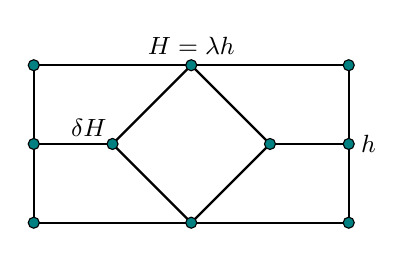
\begin{tikzpicture}
%\draw[fill=gray!23,gray!23](0,0) rectangle (5,5);
%\draw[step=0.5cm,gray,very thin] (0,0) grid (6,4); %background grid
\draw[thick] (1,1) -- (5,1) -- (5,3) -- (1,3) -- cycle;  
\draw[thick] (3,1) -- (4,2) -- (3,3) -- (2,2) -- cycle;  
\draw[thick] (1,2) -- (2,2);  
\draw[thick] (4,2) -- (5,2);  
\node[] at (5.25,2) {\small $h$};
\node[] at (3,3.25) {\small $H=\lambda h$};
\node[] at (1.7,2.2) {\small $\delta H$};
\draw[black,fill=teal] (1,1) circle (2pt);
\draw[black,fill=teal] (3,1) circle (2pt);
\draw[black,fill=teal] (5,1) circle (2pt);
\draw[black,fill=teal] (1,2) circle (2pt);
\draw[black,fill=teal] (2,2) circle (2pt);
\draw[black,fill=teal] (4,2) circle (2pt);
\draw[black,fill=teal] (5,2) circle (2pt);
\draw[black,fill=teal] (1,3) circle (2pt);
\draw[black,fill=teal] (3,3) circle (2pt);
\draw[black,fill=teal] (5,3) circle (2pt);
\end{tikzpicture}
\end{center}

The total area is 
\[
A= \lambda h \cdot h = \lambda h^2
\]
The area of the trapezes is
\[
A_{TR} = (\frac{H}{2} + \delta H)\frac12 \cdot \frac{h}{2}=\frac{\lambda h^2}{4} \left(\frac12 + \delta \right)
\]
while the area of the middle diamond is
\[
A_D = 4 \cdot \frac12 \frac{h}{2} \left(\frac{H}{2}-\delta H \right) 
= \lambda h^2 \left(\frac12 - \delta \right)
\]
We can compute $\delta$ by requiring that the trapezes and the diamond all 
have the same area, i.e.
\[
\frac{\lambda h^2}{4} (\frac12 + \delta)
=
\lambda h^2 (\frac12 - \delta)
\qquad
\Rightarrow \quad \delta = 0.3
\]
We find that the value of $\delta$ is independent of $\lambda$.

We see in the literature \cite{sten84,brfo,chba93}  that the 
macro-element is often depicted with the diamond being a square.
In this case we must have along the horizontal middle line
\[
\lambda h = 0.3 \lambda h + \frac{h}{2}+ \frac{h}{2} + 0.3 \lambda h
\qquad
\Rightarrow \quad 
\lambda=5/2
\]
The 5:2 aspect ratio macro-element guarantees equal areas and a square middle element.

But does the aspect ratio matter in practice? 
Results are shown hereunder for the D\&H benchmark:

\begin{center}
\includegraphics[width=5.7cm]{python_codes/fieldstone_78/results/exp01/stenberg_study/errors_u.pdf}
\includegraphics[width=5.7cm]{python_codes/fieldstone_78/results/exp01/stenberg_study/errors_p.pdf}
\includegraphics[width=5.7cm]{python_codes/fieldstone_78/results/exp01/stenberg_study/errors_q1.pdf}\\
{\captionfont square ($nelx=nely$): 16x16, 32x32, 48x48; 
ar ($nely/nelx=5/2$) : 10x25, 20x50, 40x100.}
\end{center}

We find that in practice this consideration does not make much of a difference,
and that the $nelx=nely$ case actually yields slightly better results.

%......................................................................
\paragraph{A note about the Le Talle m-e.}

\begin{center}
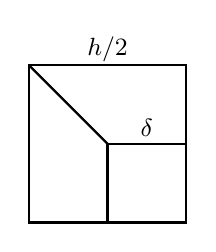
\begin{tikzpicture}
\draw[thick] (1,1) -- (3,1) -- (3,3) -- (1,3) -- cycle;  
\draw[thick] (1,3) -- (2,2);  
\draw[thick] (2,1) -- (2,2) --(3,2);  
\node[] at (2.5,2.2) {\small $\delta$};
\node[] at (2,3.2) {\small $h/2$};
\end{tikzpicture}
\end{center}

The area of the trapezes is 
\[
A_{TR}=\frac12 (\frac{h}{2}+\delta) (\frac{h}{2}-\delta) = \frac{h^2}{8}- \frac{\delta^2}{2}
\]
while the area of the square element is $A_{SQ}=\delta^2$.
When set to be equal, we arrive at
\[
\delta^2 = \frac{h}{\sqrt{12}} \simeq 0.288 h
\]


\begin{center}
\includegraphics[width=5.7cm]{python_codes/fieldstone_78/results/epsilon_studies/LT/errorss.pdf}
\end{center}





 %%%%%%%%%%%%%%%%%%%%%%%%%%%%%%%%%%%%%%%%%%%%%%%%%%%%%%%%%%%

\chapter{DG-FEM: 2D steady state diffusion \label{f79}} %%%%%%%%%%%%%%%%%%%%%%%%%%%%%%%%%%%%%%%%%%% 79
\lstinputlisting[language=bash,basicstyle=\small]{python_codes/fieldstone_79/keywords.ascii}

\begin{center}
Code at \url{https://github.com/cedrict/fieldstone/tree/master/python_codes/fieldstone_79}
\end{center}

\par\noindent\rule{\textwidth}{0.4pt}

{\sl This stone was developed in collaboration with Jort Jansen}. \index{contributors}{J. Jansen}

\par\noindent\rule{\textwidth}{0.4pt}

%%%%%%%%%%%%%%%%%%%%%%%%%%%%%%%%%%%%%%%%%%%%%%%%%%%%%%%%%%%%%%%%%%%%%%%%%%%%%%%%%%%%%%%%

Before reading what follows I urge you to go to Chapter~\ref{MMM-dgfem}. The derivations 
presented therein are long and complex, but absolutely necessary to make sense of the code.  
The code has been written for both bilinear ($Q_1$) quadrilateral elements and 
and linear ($P_1$) triangular elements. Meshes are then as follows:

\begin{center}
\includegraphics[width=10cm]{python_codes/fieldstone_79/images/grids2D_tris}\\
{\captionfont Example of a $4\times 3$ triangular mesh.}
\end{center}

\begin{center}
\includegraphics[width=10cm]{python_codes/fieldstone_79/images/grids2D_quads}\\
{\captionfont Example of a $4\times 3$ quadrilateral mesh.}
\end{center}

Contrarily to standard continuous finite elements nodes/vertices are not 
shared across elements so that the node layout is entirely based on the 
already built connectivity array {\tt icon}. Node coordinates are stored in 
{\tt xT} and {\tt yT}.

Six ascii output files are opened at the beginning of the code, and in these 
various statistics will be written out. These are 
{\sl T\_stats.ascii}, {\sl qx\_stats.ascii}, {\sl qy\_stats.ascii},
{\sl residual\_T\_stats.ascii}, {\sl residual\_qx\_stats.ascii}, and {\sl residual\_qy\_stats.ascii}.

Then a large number of arrays is declared. Then contain information that is needed 
when building the matrices and vectors later on and it is convenient to store this information
beforehand. They all start with {\tt edge} and record the normal to the edge, its center coordinates, 
its length, whether it is on the domain boundary, etc ... Because this is an educative code 
with a simple mesh topology we can directly ascribe the normals to each side. If a mesher, like 
Triangle \cite{shew14}, was used then we would need to compute the normals to each side by means
of simple geometrical considerations.

We continue to build the necessary arrays pertaining to neighbours. 
We build the {\tt edgeX\_neighb[iel]} arrays which contain the identity of the element 
on the other size of edge X of element iel.
For instance, looking at the example above of a triangular mesh, we have
\begin{lstlisting}
edge1_neighb[0]=-1
edge2_neighb[0]=1
edge3_neighb[0]=-1
...
edge1_neighb[10]=3
edge2_neighb[10]=11
edge3_neighb[10]=9
\end{lstlisting}
where the -1 value indicates that there is no element neighbour.

We then build the arrays {\tt edgeX\_neighbedge[iel]} (where X stand for 1, 2, 3, 
or 4) which stores the identity/number of the edge on the element across the common face
(if there is a neighbour).
For instance:
\begin{lstlisting}
edge1_neighbedge[10]=2
edge2_neighbedge[10]=3
edge3_neighbedge[10]=1
\end{lstlisting}


\begin{center}
\includegraphics[width=10cm]{python_codes/fieldstone_79/images/drawing}\\
{\captionfont When two triangles are neighbours (here along edge 1
of grey triangle) three configurations can occur.}
\end{center}

%............................
\paragraph{Iterative process}
Although we are solving the steady-state diffusion equation, we still need to carry out 
iterations (this is a consequence of the DG formulation itself and it is not the 
case for 'regular' finite elements).
These iterations are implemented as follows:
\begin{lstlisting}
for iter in range(0,niter):
\end{lstlisting}
where {\tt niter} is set to 100. Vector residuals are computed for $T$, $q_x$ and $q_y$. When the
infinite-norm of all three is below the tolerance {\tt tol} then the system is considered 
converged and iterations are stopped.   
For each iteration the code prints a number of helpful statistics in the terminal:
\begin{scriptsize}
\begin{verbatim}
iter=   0 : T,qx,qy (m/M)= 6.944e-03 2.053e+00 | -1.067e+01 2.054e+01 | -1.067e+01 2.054e+01 | max(resT)= 5.700e-01 (tol= 1.0e-09)
iter=   1 : T,qx,qy (m/M)= 9.982e-04 2.053e+00 | -3.991e+00 8.163e+00 | -3.991e+00 8.163e+00 | max(resT)= 7.515e-01 (tol= 1.0e-09)
iter=   2 : T,qx,qy (m/M)= 9.982e-04 2.702e+00 | -2.278e+00 3.863e+00 | -2.278e+00 3.863e+00 | max(resT)= 5.316e-01 (tol= 1.0e-09)
...
iter=  41 : T,qx,qy (m/M)= 3.473e-13 2.000e+00 | 1.000e+00 1.000e+00 | 1.000e+00 1.000e+00 | max(resT)= 1.537e-09 (tol= 1.0e-09)
iter=  42 : T,qx,qy (m/M)= 3.473e-13 2.000e+00 | 1.000e+00 1.000e+00 | 1.000e+00 1.000e+00 | max(resT)= 9.357e-10 (tol= 1.0e-09)
\end{verbatim}
\end{scriptsize}

Each iteration consists in a sweep through elements and we implement a forward-backward scheme:
even-numbered iterations got from 0 to nel-1, while odd-numbered ones go from nel-1 down to 0:
\begin{lstlisting}
if iter%2==0:
   start=0
   end=nel
   step=1
else:
   start=nel-1
   end=-1
   step=-1
\end{lstlisting}





\newpage

Explore/implement

source term
randomised nodes so no right angles




%------------------------------------------------
\subsubsection*{Experiment \#1 - testing signs} 

We define the simple temperature field 
\[
T(x,y)=x+y
\]
over a unit square domain, so that (taking $k=1$) we have
\[
q_x(x,y)=-1
\qquad
q_y(x,y)=-1
\]
I prescribe this temperature on all four sides of the domain. 

\begin{center}
\includegraphics[width=5cm]{python_codes/fieldstone_79/results/exp1/temp}
\includegraphics[width=5cm]{python_codes/fieldstone_79/results/exp1/temp2}
\end{center}


VERIFY: minus sign problem for heat fluxes ?


%------------------------------
\subsubsection*{Experiment \#2 - testing symmetry} 

On all four sides of the domain the temperature $T(x,y)=x(L_x-x)+y(L_y-y)$
is prescribed. There is no analytical solution to this problem (?) but 
it allows us to test that the solution is symmetric as expected.

\begin{center}
\includegraphics[width=5cm]{python_codes/fieldstone_79/results/exp2/temp}
\includegraphics[width=5cm]{python_codes/fieldstone_79/results/exp2/temp2}
\end{center}




 %%%%%%%%%%%%%%%%%%%%%%%%%%%%%%%%%%%%%%%%%%%%%%%%%%%%%%%%%%%

\chapter{Fortin's $Q_1^+\times P_0$ in 2D \label{f80}} %%%%%%%%%%%%%%%%%%%%%%%%%%%%%%%%%%%%%%%%%%%% 80
\lstinputlisting[language=bash,basicstyle=\small]{python_codes/fieldstone_80/keywords.key}

\begin{center}
Code at \url{https://github.com/cedrict/fieldstone/tree/master/python_codes/fieldstone_80}
\end{center}

\par\noindent\rule{\textwidth}{0.4pt}
%%%%%%%%%%%%%%%%%%%%%%%%%%%%%%%%%%%%%%%%%%%%%%%%%%%%%%%%%%%%%%%%%%%%%%%%%%%%%%%%%%%%%%%%%%%%%%

We here consider the enriched $Q_1\times P_0$ element introduced first by \textcite{fort81} (1981).
The shape functions in 2D and 3D are in derived in Section~\ref{MMM-ss:Q1pP02D} 
and Section~\ref{MMM-ss:Q1pP03D} respectively. We here only focus on the 2D variant.

The list of velocity degrees of freedom per element is as follows:
\[
\vec{\cal V} = (u_1,v_1,u_2,v_2,u_3,v_3,u_4,v_4,u_5,v_5,u_6,v_6)
\]
with the following internal numbering
\begin{verbatim}

u dofs      v dofs

4-----3     4--6--3
|     |     |     |
5     6     |     |
|     |     |     |
1-----2     1--5--2

\end{verbatim}

We start with a simple $4\times 3$ element mesh. 
Bubble $u$ dofs are represented in blue and bubble $v$ dofs are shown in green.




\begin{center}
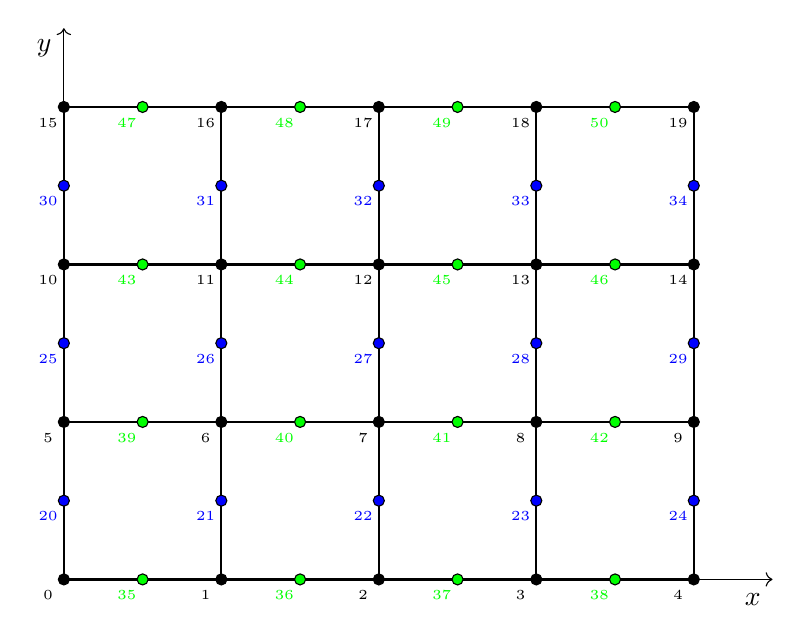
\begin{tikzpicture}
%\draw[fill=gray!23,gray!23](0,0) rectangle (10,8);
%\draw[step=0.5cm,gray,very thin] (0,0) grid (10,8); %background grid

\draw[thick] (1,1) -- (9,1) ;
\draw[thick] (1,3) -- (9,3) ;
\draw[thick] (1,5) -- (9,5) ;
\draw[thick] (1,7) -- (9,7) ;

\draw[thick] (1,1) -- (1,7) ;
\draw[thick] (3,1) -- (3,7) ;
\draw[thick] (5,1) -- (5,7) ;
\draw[thick] (7,1) -- (7,7) ;
\draw[thick] (9,1) -- (9,7) ;

\draw[black,fill=black] (1,1)   circle (2pt);
\draw[black,fill=black] (3,1)   circle (2pt);
\draw[black,fill=black] (5,1)   circle (2pt);
\draw[black,fill=black] (7,1)   circle (2pt);
\draw[black,fill=black] (9,1)   circle (2pt);

\draw[black,fill=black] (1,3)   circle (2pt);
\draw[black,fill=black] (3,3)   circle (2pt);
\draw[black,fill=black] (5,3)   circle (2pt);
\draw[black,fill=black] (7,3)   circle (2pt);
\draw[black,fill=black] (9,3)   circle (2pt);

\draw[black,fill=black] (1,5)   circle (2pt);
\draw[black,fill=black] (3,5)   circle (2pt);
\draw[black,fill=black] (5,5)   circle (2pt);
\draw[black,fill=black] (7,5)   circle (2pt);
\draw[black,fill=black] (9,5)   circle (2pt);

\draw[black,fill=black] (1,7)   circle (2pt);
\draw[black,fill=black] (3,7)   circle (2pt);
\draw[black,fill=black] (5,7)   circle (2pt);
\draw[black,fill=black] (7,7)   circle (2pt);
\draw[black,fill=black] (9,7)   circle (2pt);

\draw[black,fill=blue] (1,2) circle (2pt); 
\draw[black,fill=blue] (3,2) circle (2pt); 
\draw[black,fill=blue] (5,2) circle (2pt); 
\draw[black,fill=blue] (7,2) circle (2pt); 
\draw[black,fill=blue] (9,2) circle (2pt); 

\draw[black,fill=blue] (1,4) circle (2pt); 
\draw[black,fill=blue] (3,4) circle (2pt); 
\draw[black,fill=blue] (5,4) circle (2pt); 
\draw[black,fill=blue] (7,4) circle (2pt); 
\draw[black,fill=blue] (9,4) circle (2pt); 

\draw[black,fill=blue] (1,6) circle (2pt); 
\draw[black,fill=blue] (3,6) circle (2pt); 
\draw[black,fill=blue] (5,6) circle (2pt); 
\draw[black,fill=blue] (7,6) circle (2pt); 
\draw[black,fill=blue] (9,6) circle (2pt); 

\draw[black,fill=green] (2,1) circle (2pt); 
\draw[black,fill=green] (4,1) circle (2pt); 
\draw[black,fill=green] (6,1) circle (2pt); 
\draw[black,fill=green] (8,1) circle (2pt); 

\draw[black,fill=green] (2,3) circle (2pt); 
\draw[black,fill=green] (4,3) circle (2pt); 
\draw[black,fill=green] (6,3) circle (2pt); 
\draw[black,fill=green] (8,3) circle (2pt); 

\draw[black,fill=green] (2,5) circle (2pt); 
\draw[black,fill=green] (4,5) circle (2pt); 
\draw[black,fill=green] (6,5) circle (2pt); 
\draw[black,fill=green] (8,5) circle (2pt); 

\draw[black,fill=green] (2,7) circle (2pt); 
\draw[black,fill=green] (4,7) circle (2pt); 
\draw[black,fill=green] (6,7) circle (2pt); 
\draw[black,fill=green] (8,7) circle (2pt); 

\draw[thin,->] (9,1) -- (10,1); %x
\draw[thin,->] (1,7) -- (1,8); %y
\node[] at (9.75,0.75) {$x$};
\node[] at (0.75,7.75) {$y$};

\node[] at (0.8,0.8) {\tiny 0};
\node[] at (2.8,0.8) {\tiny 1};
\node[] at (4.8,0.8) {\tiny 2};
\node[] at (6.8,0.8) {\tiny 3};
\node[] at (8.8,0.8) {\tiny 4};
\node[] at (0.8,2.8) {\tiny 5};
\node[] at (2.8,2.8) {\tiny 6};
\node[] at (4.8,2.8) {\tiny 7};
\node[] at (6.8,2.8) {\tiny 8};
\node[] at (8.8,2.8) {\tiny 9};
\node[] at (0.8,4.8) {\tiny 10};
\node[] at (2.8,4.8) {\tiny 11};
\node[] at (4.8,4.8) {\tiny 12};
\node[] at (6.8,4.8) {\tiny 13};
\node[] at (8.8,4.8) {\tiny 14};
\node[] at (0.8,6.8) {\tiny 15};
\node[] at (2.8,6.8) {\tiny 16};
\node[] at (4.8,6.8) {\tiny 17};
\node[] at (6.8,6.8) {\tiny 18};
\node[] at (8.8,6.8) {\tiny 19};

\node[] at (0.8,1.8) {\tiny \color{blue} 20};
\node[] at (2.8,1.8) {\tiny \color{blue} 21};
\node[] at (4.8,1.8) {\tiny \color{blue} 22};
\node[] at (6.8,1.8) {\tiny \color{blue} 23};
\node[] at (8.8,1.8) {\tiny \color{blue} 24};

\node[] at (0.8,3.8) {\tiny \color{blue} 25};
\node[] at (2.8,3.8) {\tiny \color{blue} 26};
\node[] at (4.8,3.8) {\tiny \color{blue} 27};
\node[] at (6.8,3.8) {\tiny \color{blue} 28};
\node[] at (8.8,3.8) {\tiny \color{blue} 29};

\node[] at (0.8,5.8) {\tiny \color{blue} 30};
\node[] at (2.8,5.8) {\tiny \color{blue} 31};
\node[] at (4.8,5.8) {\tiny \color{blue} 32};
\node[] at (6.8,5.8) {\tiny \color{blue} 33};
\node[] at (8.8,5.8) {\tiny \color{blue} 34};

\node[] at (1.8,0.8) {\tiny \color{green} 35};
\node[] at (3.8,0.8) {\tiny \color{green} 36};
\node[] at (5.8,0.8) {\tiny \color{green} 37};
\node[] at (7.8,0.8) {\tiny \color{green} 38};

\node[] at (1.8,2.8) {\tiny \color{green} 39};
\node[] at (3.8,2.8) {\tiny \color{green} 40};
\node[] at (5.8,2.8) {\tiny \color{green} 41};
\node[] at (7.8,2.8) {\tiny \color{green} 42};

\node[] at (1.8,4.8) {\tiny \color{green} 43};
\node[] at (3.8,4.8) {\tiny \color{green} 44};
\node[] at (5.8,4.8) {\tiny \color{green} 45};
\node[] at (7.8,4.8) {\tiny \color{green} 46};

\node[] at (1.8,6.8) {\tiny \color{green} 47};
\node[] at (3.8,6.8) {\tiny \color{green} 48};
\node[] at (5.8,6.8) {\tiny \color{green} 49};
\node[] at (7.8,6.8) {\tiny \color{green} 50};

\end{tikzpicture}\\
\end{center}


For this mesh we have 

\begin{lstlisting}
nel=nelx*nely (=12) 
NP=nel (=12)
NV=nnx*nny+nnx*nely+nny*nelx (=20+16+15=51)
\end{lstlisting}

The total number of velocity dofs is 
\begin{lstlisting}
NfemV=ndofV*nnx*nny + nnx*nely + nny*nelx (=71)
\end{lstlisting}
while the total number of pressure dofs remains
\begin{lstlisting}
NfemP=NP*ndofP (=nel) 
\end{lstlisting}

What makes this element pair rather awkward to implement is the fact that 
there are two connectivity arrays {\tt iconu} and {\tt iconv}, both of size $mV\times nel$, where 
$mV=6$ is the number of nodes linked to an element for each velocity component. 
For each element, and depending on whether we are considering 
the polynomial approximation $u^h(x,y)$ or $v^h(x,y)$ in the element, there are the standard 4 $Q_1$ nodes and 2 additional 
dofs, so $mV=6$.
\begin{itemize}
\item content of {\tt iconu}
\begin{verbatim}
elt
0 | [ 0  1  6  5 20 21]
1 | [ 1  2  7  6 21 22]
2 | [ 2  3  8  7 22 23]
3 | [ 3  4  9  8 23 24]
4 | [ 5  6 11 10 25 26]
5 | [ 6  7 12 11 26 27]
6 | [ 7  8 13 12 27 28]
7 | [ 8  9 14 13 28 29]
8 | [10 11 16 15 30 31]
9 | [11 12 17 16 31 32]
10 | [12 13 18 17 32 33]
11 | [13 14 19 18 33 34]
\end{verbatim}
\item content of {\tt iconv}
\begin{verbatim}
elt
 0 | [ 0  1  6  5 35 39]
 1 | [ 1  2  7  6 36 40]
 2 | [ 2  3  8  7 37 41]
 3 | [ 3  4  9  8 38 42]
 4 | [ 5  6 11 10 39 43]
 5 | [ 6  7 12 11 40 44]
 6 | [ 7  8 13 12 41 45]
 7 | [ 8  9 14 13 42 46]
 8 | [10 11 16 15 43 47]
 9 | [11 12 17 16 44 48]
10 | [12 13 18 17 45 49]
11 | [13 14 19 18 46 50]
\end{verbatim}
\end{itemize}

The pressure field is normalised by imposing $\int_\Omega p dV=0 $ so that there is no nullspace.

%---------------------------------------------------------------
\subsection*{Donea \& Huerta manufactured solution benchmark}

The Donea \& huerta benchmark of Section~\ref{MMM-mms1} is implemented. It requires 
no-slip boundary conditions on all sides. This means that $u=0$ must be 
prescribed on the lateral boundaries, while $v=0$ is prescribed at the top and bottom, 
i.e. boundary conditions are imposed on the bubble nodes too.

\begin{center}
\includegraphics[width=8cm]{python_codes/fieldstone_80/results/dh/pressure}
\includegraphics[width=8cm]{python_codes/fieldstone_80/results/dh/pressure_error}\\
{\captionfont  opla}
\end{center}


Looking at the velocity and pressure error convergence, we see that the number of quadrature
points does not matter much, but surprisingly the lowest number of quad points seems to yield slightly
better results...
\begin{center}
\includegraphics[width=8cm]{python_codes/fieldstone_80/results/dh/errors}
\includegraphics[width=8cm]{python_codes/fieldstone_80/results/dh/vrms}\\
{\captionfont Left: Velocity and pressure error convergence as a function of resolution for 
different quadrature rules. Right: root mean square velocity.}
\end{center}

\begin{center}
\includegraphics[width=7cm]{python_codes/fieldstone_80/results/dh/vel}
\includegraphics[width=7cm]{python_codes/fieldstone_80/results/dh/vel_error}\\
\includegraphics[width=7cm]{python_codes/fieldstone_80/results/dh/u_dofs}
\includegraphics[width=7cm]{python_codes/fieldstone_80/results/dh/v_dofs}\\
{\captionfont Top row: velocity and velocity error. Bottom row: $u$ and 
$v$ plotted on their respective meshes.}
\end{center}

%---------------------------------------------------------------
\subsection*{The aquarium}

No-slip boundary conditions are prescribed on all sides. Density and viscosity are 1.
Gravity is $\vec{g}=-\vec{e}_y$. 

We recover a linear pressure profile as expected, that is very accurate:

\begin{center}
\includegraphics[width=7.5cm]{python_codes/fieldstone_80/results/aquarium/p}
\includegraphics[width=7.5cm]{python_codes/fieldstone_80/results/aquarium/p_error}\\
{\captionfont Left: pressure profile; Right: pressure profile error}
\end{center}

We can also record the root mean square velocity as a function of the resolution $h$
and we find that the velocity is (as expected) zero (down to machine precision):
\begin{center}
\includegraphics[width=9cm]{python_codes/fieldstone_80/results/aquarium/vrms}
\end{center}


%---------------------------------------------------------------
\subsection*{The lid driven cavity}

This is the non leaky lid driven cavity, i.e. the velocity at the top left and right corner 
is set to zero. No slip are imposed on all three other boundaries. 
The pressure field does not showcase any checkerboard mode. 

\begin{center}
\includegraphics[width=8cm]{python_codes/fieldstone_80/results/ldc/vel}
\includegraphics[width=8cm]{python_codes/fieldstone_80/results/ldc/p}\\
\includegraphics[width=8cm]{python_codes/fieldstone_80/results/ldc/u_dofs}
\includegraphics[width=8cm]{python_codes/fieldstone_80/results/ldc/v_dofs}
{\captionfont 64x64}
\end{center}

\begin{center}
\includegraphics[width=8cm]{python_codes/fieldstone_80/results/ldc/p_top}
\includegraphics[width=8cm]{python_codes/fieldstone_80/results/ldc/vrms}
\end{center}

%---------------------------------------------------------------
\subsection*{The regularised lid driven cavity}

The velocity at the top is $u(x,y)=16x^2(1-x)^2$. 

\begin{center}
\includegraphics[width=8cm]{python_codes/fieldstone_80/results/ldc_reg/vel}
\includegraphics[width=8cm]{python_codes/fieldstone_80/results/ldc_reg/p}\\
{\captionfont Resolution 96x96}
\end{center}

The pressure field converges to a unique solution and no visible checkerboard signal.
\begin{center}
\includegraphics[width=12cm]{python_codes/fieldstone_80/results/ldc_reg/p_top.pdf}\\
{\captionfont Elemental pressure at the top of the domain.}
\end{center}



%---------------------------------------------------------------
\subsection*{Dohrmann \& Bochev manufactured solution}

This benchmark is defined in Section~\ref{MMM-ss:mms2}.

\begin{center}
\includegraphics[width=8cm]{python_codes/fieldstone_80/results/db2d/vel}
\includegraphics[width=8cm]{python_codes/fieldstone_80/results/db2d/p}
\end{center}


\begin{center}
\includegraphics[width=8cm]{python_codes/fieldstone_80/results/db2d/errors}
\includegraphics[width=8cm]{python_codes/fieldstone_80/results/db2d/vrms}\\
{\captionfont Left: Velocity and pressure error convergence; Right: root mean square velocity
as a function of mesh size.}
\end{center}


%---------------------------------------------------------------
\subsection*{Stokes sphere}

Sphere is placed in the middle with radius 0.123, free slip boundary conditions on all sides. 
Viscosity is constant in the domain. 

\begin{center}
\includegraphics[width=5.6cm]{python_codes/fieldstone_80/results/sphere/rho_g}
\includegraphics[width=5.6cm]{python_codes/fieldstone_80/results/sphere/vel}
\includegraphics[width=5.6cm]{python_codes/fieldstone_80/results/sphere/p}\\
\includegraphics[width=5.6cm]{python_codes/fieldstone_80/results/sphere/u_dofs}
\includegraphics[width=5.6cm]{python_codes/fieldstone_80/results/sphere/v_dofs}\\
{\captionfont velocity and pressure fields for $\delta \rho=0.001$. 96x96 elements.}
\end{center}

\begin{center}
\includegraphics[width=10cm]{python_codes/fieldstone_80/results/sphere/vrms}\\
{\captionfont Root mean square velocity for $\delta \rho=0.001$, for both full density and reduced 
density models.}
\end{center}


%---------------------------------------------------------------
\subsection*{SolVi}

\begin{center}
\includegraphics[width=5cm]{python_codes/fieldstone_80/results/solvi/vel}
\includegraphics[width=5cm]{python_codes/fieldstone_80/results/solvi/vel_th}
\includegraphics[width=5cm]{python_codes/fieldstone_80/results/solvi/vel_error}\\
\includegraphics[width=5cm]{python_codes/fieldstone_80/results/solvi/p}
\includegraphics[width=5cm]{python_codes/fieldstone_80/results/solvi/p_th}
\includegraphics[width=5cm]{python_codes/fieldstone_80/results/solvi/p_error}\\
{\captionfont 96x96 elements, nqperdim=5. Left to right: computed field, analytical solution, error between both.
Top row field is velocity, bottom row field is pressure.}
\end{center}


\begin{center}
\includegraphics[width=7cm]{python_codes/fieldstone_80/results/solvi/vrms}
\includegraphics[width=7cm]{python_codes/fieldstone_80/results/solvi/errors}\\
\includegraphics[width=5cm]{python_codes/fieldstone_80/results/solvi/stats_u}
\includegraphics[width=5cm]{python_codes/fieldstone_80/results/solvi/stats_v}
\includegraphics[width=5cm]{python_codes/fieldstone_80/results/solvi/stats_p}\\
\end{center}

What is surprising is the fact that L2-norm pressure error is best for nq=2 but the min/max values of pressure
are best for $nq>2$.


\newpage
%---------------------------------------------------------------
\subsection*{SolCx}

See Stone 5 and Section~\ref{MMM-sec:geobench}.

\begin{center}
\includegraphics[width=8cm]{python_codes/fieldstone_80/results/solcx/vrms}
\includegraphics[width=8cm]{python_codes/fieldstone_80/results/solcx/errors}\\
\includegraphics[width=5cm]{python_codes/fieldstone_80/results/solcx/stats_u}
\includegraphics[width=5cm]{python_codes/fieldstone_80/results/solcx/stats_v}
\includegraphics[width=5cm]{python_codes/fieldstone_80/results/solcx/stats_p}\\
\end{center}


\newpage
%---------------------------------------------------------------
\subsection*{Sinking block}

This experiment is fully described in Section~\ref{MMM-sec:sinker}.
It is run at resolutions such that the boundaries of the elements are aligned with the sides of the block.

\begin{center}
\includegraphics[width=7.7cm]{python_codes/fieldstone_80/results/block/results_v}
\includegraphics[width=7.7cm]{python_codes/fieldstone_80/results/block/pline}\\
{\captionfont Left: normalised velocity as a function of the viscosity ratio. Right: 
nodal pressure profile on the $x=L_x/2$ line.}
\end{center}


\begin{center}
\includegraphics[width=7.cm]{python_codes/fieldstone_80/results/block/rhog}
\includegraphics[width=7.cm]{python_codes/fieldstone_80/results/block/vel}\\
\includegraphics[width=7.cm]{python_codes/fieldstone_80/results/block/u}
\includegraphics[width=7.cm]{python_codes/fieldstone_80/results/block/v}\\
\includegraphics[width=7.cm]{python_codes/fieldstone_80/results/block/p}
\includegraphics[width=7.cm]{python_codes/fieldstone_80/results/block/q}\\
{\captionfont Resolution 128x128}
\end{center}
The elemental pressure does not showcase any sign of checkerboard and converges to a unique solution. 


%---------------------------------------------------------------
\subsection*{Conclusion}

This element is very much usable: it is accurate for both buoyancy-driven problems and 
analytical solutions. 
However, one last set of tests should be carried out with regards to its implementation 
and usability when the mesh deforms, or when an annulus geometry is used.
 %%%%%%%%%%%%%%%%%%%%%%%%%%%%%%%%%%%%%%%%%%%%%%%%%%%%%%%%%%%

\chapter{Fortin's $Q_1^+\times P_0$ in 3D \label{f81}} %%%%%%%%%%%%%%%%%%%%%%%%%%%%%%%%%%%%%%%%%%%% 81
\lstinputlisting[language=bash,basicstyle=\small]{python_codes/fieldstone_81/keywords.ascii}

\begin{center}
Code at \url{https://github.com/cedrict/fieldstone/tree/master/python_codes/fieldstone_81}
\end{center}

\par\noindent\rule{\textwidth}{0.4pt}
%%%%%%%%%%%%%%%%%%%%%%%%%%%%%%%%%%%%%%%%%%%%%%%%%%%%%%%%%%%%%%%%%%%%%%%%%%%%%%%%%%%%%%%%%%%%%%

This element is presented in \textcite{fort81} (1981). It is 
also mentioned in \textcite{dhhu86} (1986) and called 'H8N' and 
proved to be LBB-stable in the appendix.

\begin{center}
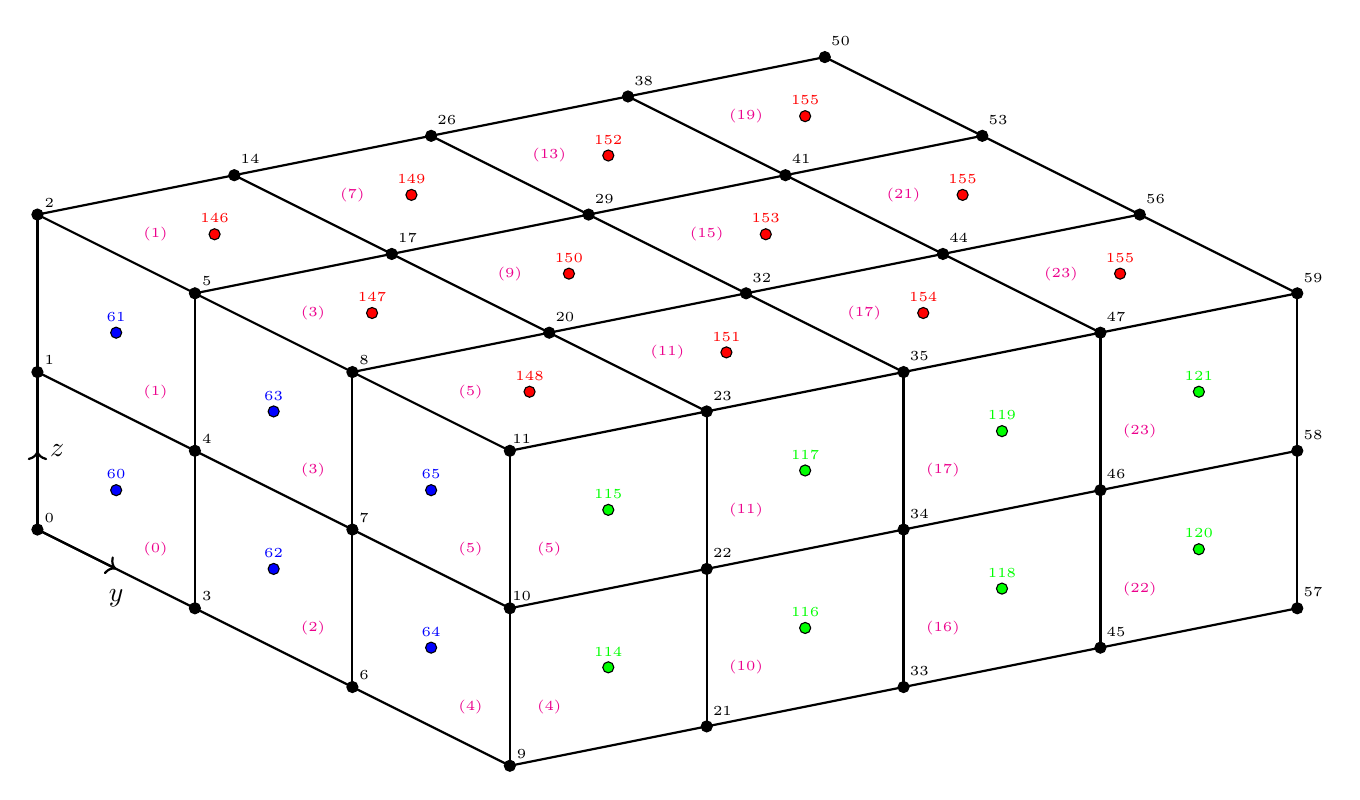
\begin{tikzpicture}
%\draw[fill=gray!23,gray!23](0,0) rectangle (16,9);
%\draw[step=0.5cm,gray,very thin] (0,0) grid (16,9); %background grid

\draw[thick] (0,3) -- (6,0) ;
\draw[thick] (0,5) -- (6,2) ;
\draw[thick] (0,7) -- (6,4) ;

\draw[thick] (2.5,7.5) -- (8.5,4.5) ;
\draw[thick] (5,8) -- (11,5) ;
\draw[thick] (7.5,8.5) -- (13.5,5.5) ;
\draw[thick] (10,9) -- (16,6) ;

\draw[thick] (0,3) -- (0,7) ;
\draw[thick] (2,2) -- (2,6) ;
\draw[thick] (4,1) -- (4,5) ;
\draw[thick] (6,0) -- (6,4) ;

\draw[thick] (0,7) -- (10,9) ;
\draw[thick] (2,6) -- (12,8) ;
\draw[thick] (4,5) -- (14,7) ;
\draw[thick] (6,4) -- (16,6) ;

\draw[thick] (6,2) -- (16,4) ;
\draw[thick] (6,0) -- (16,2) ;

\draw[thick] (8.5,0.5) -- (8.5,4.5) ;
\draw[thick] (11,1) -- (11,5) ;
\draw[thick] (13.5,1.5) -- (13.5,5.5) ;
\draw[thick] (16,2) -- (16,6) ;

\draw[black,fill=black] (0,3)   circle (2pt); \node[] at (0.15,3.15) {\tiny 0};
\draw[black,fill=black] (0,5)   circle (2pt); \node[] at (0.15,5.15) {\tiny 1};
\draw[black,fill=black] (0,7)   circle (2pt); \node[] at (0.15,7.15) {\tiny 2};

\draw[black,fill=black] (2,2)   circle (2pt); \node[] at (2.15,2.15) {\tiny 3};
\draw[black,fill=black] (2,4)   circle (2pt); \node[] at (2.15,4.15) {\tiny 4};
\draw[black,fill=black] (2,6)   circle (2pt); \node[] at (2.15,6.15) {\tiny 5};

\draw[black,fill=black] (4,1)   circle (2pt); \node[] at (4.15,1.15) {\tiny 6};
\draw[black,fill=black] (4,3)   circle (2pt); \node[] at (4.15,3.15) {\tiny 7};
\draw[black,fill=black] (4,5)   circle (2pt); \node[] at (4.15,5.15) {\tiny 8};

\draw[black,fill=black] (6,0)   circle (2pt); \node[] at (6.15,0.15) {\tiny 9};
\draw[black,fill=black] (6,2)   circle (2pt); \node[] at (6.15,2.15) {\tiny 10};
\draw[black,fill=black] (6,4)   circle (2pt); \node[] at (6.15,4.15) {\tiny 11};

\draw[black,fill=black] (8.5,0.5)   circle (2pt);  \node[] at (8.7,0.7) {\tiny 21};
\draw[black,fill=black] (8.5,2.5)   circle (2pt);  \node[] at (8.7,2.7) {\tiny 22};
\draw[black,fill=black] (8.5,4.5)   circle (2pt);  \node[] at (8.7,4.7) {\tiny 23};

\draw[black,fill=black] (11,1)   circle (2pt); \node[] at (11.2,1.2) {\tiny 33};
\draw[black,fill=black] (11,3)   circle (2pt); \node[] at (11.2,3.2) {\tiny 34};
\draw[black,fill=black] (11,5)   circle (2pt); \node[] at (11.2,5.2) {\tiny 35};

\draw[black,fill=black] (13.5,1.5)   circle (2pt); \node[] at (13.7,1.7) {\tiny 45};
\draw[black,fill=black] (13.5,3.5)   circle (2pt); \node[] at (13.7,3.7) {\tiny 46};
\draw[black,fill=black] (13.5,5.5)   circle (2pt); \node[] at (13.7,5.7) {\tiny 47};

\draw[black,fill=black] (16,2)   circle (2pt); \node[] at (16.2,2.2) {\tiny 57};
\draw[black,fill=black] (16,4)   circle (2pt); \node[] at (16.2,4.2) {\tiny 58};
\draw[black,fill=black] (16,6)   circle (2pt); \node[] at (16.2,6.2) {\tiny 59};

\draw[black,fill=black] (6.5,5.5)  circle (2pt); \node[] at (6.7,5.7) {\tiny 20};
\draw[black,fill=black] (9,6)      circle (2pt); \node[] at (9.2,6.2) {\tiny 32};
\draw[black,fill=black] (11.5,6.5) circle (2pt); \node[] at (11.7,6.7) {\tiny 44};
\draw[black,fill=black] (14,7)     circle (2pt); \node[] at (14.2,7.2) {\tiny 56};

\draw[black,fill=black] (4.5,6.5) circle (2pt); \node[] at (4.7,6.7) {\tiny 17};
\draw[black,fill=black] (7,7)     circle (2pt); \node[] at (7.2,7.2) {\tiny 29};
\draw[black,fill=black] (9.5,7.5) circle (2pt); \node[] at (9.7,7.7) {\tiny 41};
\draw[black,fill=black] (12,8)    circle (2pt); \node[] at (12.2,8.2) {\tiny 53};

\draw[black,fill=black] (2.5,7.5) circle (2pt); \node[] at (2.7,7.7) {\tiny 14};
\draw[black,fill=black] (5,8)     circle (2pt); \node[] at (5.2,8.2) {\tiny 26};
\draw[black,fill=black] (7.5,8.5) circle (2pt); \node[] at (7.7,8.7) {\tiny 38};
\draw[black,fill=black] (10,9)    circle (2pt); \node[] at (10.2,9.2) {\tiny 50};

\draw[black,fill=blue] (1,3.5) circle (2pt); \node[] at (1,3.7) {\tiny \color{blue} 60};
\draw[black,fill=blue] (1,5.5) circle (2pt); \node[] at (1,5.7) {\tiny \color{blue} 61};
\draw[black,fill=blue] (3,2.5) circle (2pt); \node[] at (3,2.7) {\tiny \color{blue} 62};
\draw[black,fill=blue] (3,4.5) circle (2pt); \node[] at (3,4.7) {\tiny \color{blue} 63};
\draw[black,fill=blue] (5,1.5) circle (2pt); \node[] at (5,1.7) {\tiny \color{blue} 64};
\draw[black,fill=blue] (5,3.5) circle (2pt); \node[] at (5,3.7) {\tiny \color{blue} 65};

\draw[black,fill=green](7.25,1.25) circle (2pt);\node[] at (7.25,1.45){\tiny\color{green}114};
\draw[black,fill=green](7.25,3.25) circle (2pt);\node[] at (7.25,3.45){\tiny\color{green}115};
\draw[black,fill=green](9.75,1.75) circle (2pt);\node[] at (9.75,1.95){\tiny\color{green}116};
\draw[black,fill=green](9.75,3.75) circle (2pt);\node[] at (9.75,3.95){\tiny\color{green}117};
\draw[black,fill=green](12.25,2.25) circle (2pt);\node[] at (12.25,2.45){\tiny\color{green}118};
\draw[black,fill=green](12.25,4.25) circle (2pt);\node[] at (12.25,4.45){\tiny\color{green}119};
\draw[black,fill=green](14.75,2.75) circle (2pt);\node[] at (14.75,2.95){\tiny\color{green}120};
\draw[black,fill=green](14.75,4.75) circle (2pt);\node[] at (14.75,4.95){\tiny\color{green}121};

\draw[black,fill=red] (2.25,6.75) circle (2pt); \node[] at (2.25,6.95) {\tiny \color{red} 146};
\draw[black,fill=red] (4.25,5.75) circle (2pt); \node[] at (4.25,5.95) {\tiny \color{red} 147};
\draw[black,fill=red] (6.25,4.75) circle (2pt); \node[] at (6.25,4.95) {\tiny \color{red} 148};

\draw[black,fill=red] (4.75,7.25) circle (2pt); \node[] at (4.75,7.45) {\tiny \color{red} 149};
\draw[black,fill=red] (6.75,6.25) circle (2pt); \node[] at (6.75,6.45) {\tiny \color{red} 150};
\draw[black,fill=red] (8.75,5.25) circle (2pt); \node[] at (8.75,5.45) {\tiny \color{red} 151};

\draw[black,fill=red] (7.25,7.75) circle (2pt); \node[] at (7.25,7.95) {\tiny \color{red} 152};
\draw[black,fill=red] (9.25,6.75) circle (2pt); \node[] at (9.25,6.95) {\tiny \color{red} 153};
\draw[black,fill=red] (11.25,5.75) circle (2pt); \node[] at (11.25,5.95) {\tiny \color{red} 154};

\draw[black,fill=red] (9.75,8.25) circle (2pt); \node[] at (9.75,8.45) {\tiny \color{red} 155};
\draw[black,fill=red] (11.75,7.25) circle (2pt); \node[] at (11.75,7.45) {\tiny \color{red} 155};
\draw[black,fill=red] (13.75,6.25) circle (2pt); \node[] at (13.75,6.45) {\tiny \color{red} 155};

\node[] at (1.5,2.75) {\tiny \color{magenta} (0)};
\node[] at (1.5,4.75) {\tiny \color{magenta} (1)};
\node[] at (3.5,1.75) {\tiny \color{magenta} (2)};
\node[] at (3.5,3.75) {\tiny \color{magenta} (3)};
\node[] at (5.5,0.75) {\tiny \color{magenta} (4)};
\node[] at (5.5,2.75) {\tiny \color{magenta} (5)};

\node[] at (6.5,0.75) {\tiny \color{magenta} (4)};
\node[] at (6.5,2.75) {\tiny \color{magenta} (5)};
\node[] at (9,1.25) {\tiny \color{magenta} (10)};
\node[] at (9,3.25) {\tiny \color{magenta} (11)};
\node[] at (11.5,1.75) {\tiny \color{magenta} (16)};
\node[] at (11.5,3.75) {\tiny \color{magenta} (17)};
\node[] at (14,2.25) {\tiny \color{magenta} (22)};
\node[] at (14,4.25) {\tiny \color{magenta} (23)};

\node[] at (5.5,4.75) {\tiny \color{magenta} (5)};
\node[] at (8,5.25) {\tiny \color{magenta} (11)};
\node[] at (10.5,5.75) {\tiny \color{magenta} (17)};
\node[] at (13,6.25) {\tiny \color{magenta} (23)};

\node[] at (3.5,5.75) {\tiny \color{magenta} (3)};
\node[] at (6,6.25) {\tiny \color{magenta} (9)};
\node[] at (8.5,6.75) {\tiny \color{magenta} (15)};
\node[] at (11,7.25) {\tiny \color{magenta} (21)};

\node[] at (1.5,6.75) {\tiny \color{magenta} (1)};
\node[] at (4,7.25) {\tiny \color{magenta} (7)};
\node[] at (6.5,7.75) {\tiny \color{magenta} (13)};
\node[] at (9,8.25) {\tiny \color{magenta} (19)};

\draw[thick,->] (0,3) -- (0,4); %x
\draw[thick,->] (0,3) -- (1,2.5); %y
\node[] at (1,2.125) {$y$};
\node[] at (0.25,4) {$z$};

\end{tikzpicture}\\
{\captionfont Example of a simple 4x3x2 mesh. Additional face dofs are indicated in colour.}
\end{center}

Each element has 
\begin{itemize}
\item 8+2 u dofs
\item 8+2 v dofs
\item 8+2 w dofs
\end{itemize}

Setting nelx=4, nely=3 and nelz=2, we can print the three connectivity arrays\footnote{it is the simplest way I found to account 
for the additional dofs in the three dimensions: a connectivity array per dimension.}:

\begin{itemize}
\item iconu:

\begin{verbatim}
0 [ 0 12 15  3  1 13 16  4 60 66]
1 [ 1 13 16  4  2 14 17  5 61 67]
2 [ 3 15 18  6  4 16 19  7 62 68]
3 [ 4 16 19  7  5 17 20  8 63 69]
4 [ 6 18 21  9  7 19 22 10 64 70]
5 [ 7 19 22 10  8 20 23 11 65 71]
6 [12 24 27 15 13 25 28 16 66 72]
7 [13 25 28 16 14 26 29 17 67 73]
8 [15 27 30 18 16 28 31 19 68 74]
9 [16 28 31 19 17 29 32 20 69 75]
10 [18 30 33 21 19 31 34 22 70 76]
11 [19 31 34 22 20 32 35 23 71 77]
12 [24 36 39 27 25 37 40 28 72 78]
13 [25 37 40 28 26 38 41 29 73 79]
14 [27 39 42 30 28 40 43 31 74 80]
15 [28 40 43 31 29 41 44 32 75 81]
16 [30 42 45 33 31 43 46 34 76 82]
17 [31 43 46 34 32 44 47 35 77 83]
18 [36 48 51 39 37 49 52 40 78 84]
19 [37 49 52 40 38 50 53 41 79 85]
20 [39 51 54 42 40 52 55 43 80 86]
21 [40 52 55 43 41 53 56 44 81 87]
22 [42 54 57 45 43 55 58 46 82 88]
23 [43 55 58 46 44 56 59 47 83 89]
\end{verbatim}

\item iconv:
\begin{verbatim}
0 [ 0 12 15  3  1 13 16  4 90 98]
1 [ 1 13 16  4  2 14 17  5 91 99]
2 [  3  15  18   6   4  16  19   7  98 106]
3 [  4  16  19   7   5  17  20   8  99 107]
4 [  6  18  21   9   7  19  22  10 106 114]
5 [  7  19  22  10   8  20  23  11 107 115]
6 [ 12  24  27  15  13  25  28  16  92 100]
7 [ 13  25  28  16  14  26  29  17  93 101]
8 [ 15  27  30  18  16  28  31  19 100 108]
9 [ 16  28  31  19  17  29  32  20 101 109]
10 [ 18  30  33  21  19  31  34  22 108 116]
11 [ 19  31  34  22  20  32  35  23 109 117]
12 [ 24  36  39  27  25  37  40  28  94 102]
13 [ 25  37  40  28  26  38  41  29  95 103]
14 [ 27  39  42  30  28  40  43  31 102 110]
15 [ 28  40  43  31  29  41  44  32 103 111]
16 [ 30  42  45  33  31  43  46  34 110 118]
17 [ 31  43  46  34  32  44  47  35 111 119]
18 [ 36  48  51  39  37  49  52  40  96 104]
19 [ 37  49  52  40  38  50  53  41  97 105]
20 [ 39  51  54  42  40  52  55  43 104 112]
21 [ 40  52  55  43  41  53  56  44 105 113]
22 [ 42  54  57  45  43  55  58  46 112 120]
23 [ 43  55  58  46  44  56  59  47 113 121]
\end{verbatim}

\item iconw:
\begin{verbatim}
0 [  0  12  15   3   1  13  16   4 122 134]
1 [  1  13  16   4   2  14  17   5 134 146]
2 [  3  15  18   6   4  16  19   7 123 135]
3 [  4  16  19   7   5  17  20   8 135 147]
4 [  6  18  21   9   7  19  22  10 124 136]
5 [  7  19  22  10   8  20  23  11 136 148]
6 [ 12  24  27  15  13  25  28  16 125 137]
7 [ 13  25  28  16  14  26  29  17 137 149]
8 [ 15  27  30  18  16  28  31  19 126 138]
9 [ 16  28  31  19  17  29  32  20 138 150]
10 [ 18  30  33  21  19  31  34  22 127 139]
11 [ 19  31  34  22  20  32  35  23 139 151]
12 [ 24  36  39  27  25  37  40  28 128 140]
13 [ 25  37  40  28  26  38  41  29 140 152]
14 [ 27  39  42  30  28  40  43  31 129 141]
15 [ 28  40  43  31  29  41  44  32 141 153]
16 [ 30  42  45  33  31  43  46  34 130 142]
17 [ 31  43  46  34  32  44  47  35 142 154]
18 [ 36  48  51  39  37  49  52  40 131 143]
19 [ 37  49  52  40  38  50  53  41 143 155]
20 [ 39  51  54  42  40  52  55  43 132 144]
21 [ 40  52  55  43  41  53  56  44 144 156]
22 [ 42  54  57  45  43  55  58  46 133 145]
23 [ 43  55  58  46  44  56  59  47 145 157]
\end{verbatim}

\end{itemize}


\begin{center}
a)\includegraphics[width=5.6cm]{python_codes/fieldstone_81/results/matrix4}
b)\includegraphics[width=5.6cm]{python_codes/fieldstone_81/results/matrix8}
c)\includegraphics[width=5.6cm]{python_codes/fieldstone_81/results/matrix12}\\
d)\includegraphics[width=5.6cm]{python_codes/fieldstone_81/results/matrix16}
e)\includegraphics[width=5.6cm]{python_codes/fieldstone_81/results/matrix20}
f)\includegraphics[width=5.6cm]{python_codes/fieldstone_81/results/matrix24}\\
{\captionfont non-zero pattern of the assembled Stokes matrix for $8^3$ (a), 
$12^3$ (b), $16^3$ (c) and $20^3$ (d) meshes.}
\end{center}
This is bad news: a renumbering of the nodes/dofs would be beneficial so as to reduce the 
skyline of the matrix. 

%----------------------------------------------------
\subsection*{Manufactured solution ({\tt bench=1})}

This benchmark is presented in Section~\ref{MMM-mms3} and is called the 
'Burstedde' benchmark in the ASPECT manual after 
the paper by \textcite{busa13} (2013), although it originates in \textcite{dobo04} (2004). 
It was run with 3 different quadrature levels, $nq=2^3,3^3,4^3$. 
Unfortunately a resolution $24\times 24\times 24$ is the maximum which can be run as demonstrated 
by the following table:

\begin{center}
\begin{tabular}{llll}
\hline
resolution &Nfem           &build (s) &solve(s) \\
\hline\hline
12x12x12   &12207+1728     &21        &5.4\\
16x16x16   &27795+4096     &49        &40\\
20x20x20   &52983+8000     &98.3      &414\\
21x21x21   &61050+9261     &130       &753 \\
22x22x22   &69897+10648    &144       &1213\\
24x24x24   &90075+13824    &173       &2481\\
\hline
\end{tabular}
\end{center}
 
We recover a quadratic convergence for the velocity error and a linear convergence for the pressure error, 
similarly to the $Q_1\times P_0$ element:

\begin{center}
\includegraphics[width=10cm]{python_codes/fieldstone_81/results/bench1/conv.pdf}
\end{center}

It appears that a $2 \times 2\times 2$ is sufficient and yields the best results.

%----------------------------------------------------
\subsection*{Horizontal shear ({\tt bench=2})}

Gravity is set to zero so that density values are irrelevant. Viscosity is set to 1.
Velocity boundary conditions $\frac12-z,0,0$ are prescribed at the top and bottom, 
while the side boundaries are left free. We expect this same velocity field everywhere in the 
domain and given the pressure normalisation a zero pressure in the domain. 

\begin{center}
\includegraphics[width=8cm]{python_codes/fieldstone_81/results/bench2/vel}
\includegraphics[width=8cm]{python_codes/fieldstone_81/results/bench2/press}\\
\includegraphics[width=5cm]{python_codes/fieldstone_81/results/bench2/u}
\includegraphics[width=5cm]{python_codes/fieldstone_81/results/bench2/v}
\includegraphics[width=5cm]{python_codes/fieldstone_81/results/bench2/w}
\end{center}

%----------------------------------------------------
\subsection*{Stokes sphere benchmark ({\tt bench=3})}

It is described in Section~\ref{MMM-ss:stokes_sphere3D}. We here focus on the 'NS' case, i.e. no slip 
boundary conditions are prescribed on all six faces. Unfortunately the resolution is so limited 
that it is hard to really see a convergence in the results.

\begin{center}
\includegraphics[width=5.5cm]{python_codes/fieldstone_81/results/bench3/u}
\includegraphics[width=5.5cm]{python_codes/fieldstone_81/results/bench3/v}
\includegraphics[width=5.5cm]{python_codes/fieldstone_81/results/bench3/w}\\
\includegraphics[width=5.5cm]{python_codes/fieldstone_81/results/bench3/vel}
\includegraphics[width=5.5cm]{python_codes/fieldstone_81/results/bench3/vrms}
\includegraphics[width=5.5cm]{python_codes/fieldstone_81/results/bench3/press}
\end{center}


 %%%%%%%%%%%%%%%%%%%%%%%%%%%%%%%%%%%%%%%%%%%%%%%%%%%%%%%%%%%

\chapter{The 3D MINI element with 2 bubble functions \label{f82}} %%%%%%%%%%%%%%%%%%%%%%%%%%%%%%%%% 82
%\noindent
\includegraphics[height=1.25cm]{images/pictograms/benchmark}
\includegraphics[height=1.25cm]{images/pictograms/FEM}
\includegraphics[height=1.25cm]{images/pictograms/3d}
\includegraphics[height=1.25cm]{images/pictograms/paraview}

%%%%%%%%%%%%%%%%%%%%%%%%%%%%%%%%%%%%%%%%%%%%%%%%%%%%%%%%%%%%%%%%%%%%%%%%%%%%%%%%%%%%%%%%%%%%%%%%%%%

\begin{flushright} {\tiny {\color{gray} python\_codes/fieldstone\_82/text.tex}} \end{flushright}

\lstinputlisting[language=bash,basicstyle=\small]{python_codes/fieldstone_82/keywords.key}

\par\noindent\rule{\textwidth}{0.4pt}

\begin{center}
\inpython
{\small Code: \url{https://github.com/cedrict/fieldstone/tree/master/python_codes/fieldstone_82}}
\end{center}

\par\noindent\rule{\textwidth}{0.4pt}

{\bf \color{teal} Purpose}: implement and document the $Q_1^{++}\times Q_1$ element.

\index{stopics}{$Q_1^{++} \times Q_1$}

\par\noindent\rule{\textwidth}{0.4pt}
%%%%%%%%%%%%%%%%%%%%%%%%%%%%%%%%%%%%%%%%%%%%%%%%%%%%%%%%%%%%%%%%%%%%%%%%%%%%%%%%%%%%%%%%%%%%%%%%%%%

The basis functions for this element is presented in Section~\ref{MMM-ss:Q1Q1bb_3D}.
This element is presented in \textcite{kahp20} (2020). 

There are two bubble functions/nodes per element so we then have 
\begin{lstlisting}
NV=nnx*nny*nnz+2*nel 
NP=nnx*nny*nnz
\end{lstlisting}
For a $8\times 8 \times 8=512$ element grid, there are $9^3=729$ nodes, and 1024 bubble nodes.
We then have $3\cdot 729=2157$ $Q_1$ velocity dofs and 3072 velocity dofs attached 
to the bubbles.
Since the bubble nodes are stored last the structure of the matrix is as follows:
\begin{center}
\includegraphics[width=7cm]{python_codes/fieldstone_82/results/matrix_8x8x8_bef_bc}
\includegraphics[width=7cm]{python_codes/fieldstone_82/results/matrix_8x8x8_aft_bc}\\
{\captionfont Sparsity pattern of the matrix for a 8x8x8 grid.
NV= 1753, NP=729.\\ Left:
before boundary conditions are applied. 
Right: after boundary conditions are applied.} 
\end{center}

%......................................
\subsection*{Manufactured solution (bench=1)}

This benchmark begins by postulating a polynomial solution 
to the 3D Stokes equation (see Dohrmann \& Bochev (2004) \cite{dobo04}):
\begin{equation}
\vec{\upnu}(x,y,z)
=
\left(
\begin{array}{c}
x+x^2+xy+x^3y \\
y + xy + y^2 + x^2 y^2\\
-2z - 3xz - 3yz - 5x^2 yz
\end{array}
\right)
\label{eqbur2}
\end{equation}
and
\begin{equation}
p(x,y,z) = xyz + x^3 y^3z - 5/32
\end{equation}
The corresponding right-hand side is computed in Section~\ref{MMM-mms3}.
The domain is a unit cube and velocity boundary conditions
simply use Eq.~\eqref{eqbur2}.
Note that the pressure fulfills $\int_\Omega p(x,y,z) dV = 0.$

\begin{center}
\includegraphics[width=8cm]{python_codes/fieldstone_82/results/bench1/vrms.pdf}
\includegraphics[width=8cm]{python_codes/fieldstone_82/results/bench1/conv.pdf}\\
{\captionfont Results obtained for three levels of quadrature, with $\beta=0$ (i.e.
viscosity is constant and equal to 1).}
\end{center}

Somewhat surprisingly, the pressure convergence is not exactly quadratic but seems to be
around 1.8. Also, the $2\times 2\times 2$ 
quadrature yields better results than the $3\times 3\times 3$ or $4\times 4 \times 4$.

%......................................
\subsection*{Horizontal shear (bench=2)}

This is a simple kinematical test: gravity is set to zero, no boundary 
conditions on the sides and $\vec\upnu=(-1,0,0)$ prescribed on the top, and 
$\vec\upnu=(+1,0,0)$ prescribed on the bottom.

\begin{center}
\includegraphics[width=8cm]{python_codes/fieldstone_82/results/bench2/vel}
\includegraphics[width=8cm]{python_codes/fieldstone_82/results/bench2/press}\\
{\captionfont $20\times 20 \times 20$ mesh.} 
\end{center}

%......................................
\subsection*{Stokes sphere (bench=3)}

This is the benchmark of Section~\ref{MMM-ss:stokes_sphere3D}.
A sphere of radius 0.123456789 is placed in the middle of the domain. 
It has a density excess $\delta\rho=0.01$
with respect to the surrounding fluid which has a density $\rho_{fluid}=1$. 
The sphere viscosity is 1000 while the fluid viscosity is 1.
Boundary conditions are no slip on all sides. Gravity is $\vec{g}=-\vec{e}_z$.

\begin{center}
\includegraphics[width=5cm]{python_codes/fieldstone_82/results/bench3/grid.png}
\includegraphics[width=5cm]{python_codes/fieldstone_82/results/bench3/vel.png}
\includegraphics[width=5cm]{python_codes/fieldstone_82/results/bench3/press.png}\\
\includegraphics[width=5cm]{python_codes/fieldstone_82/results/bench3/u.png}
\includegraphics[width=5cm]{python_codes/fieldstone_82/results/bench3/v.png}
\includegraphics[width=5cm]{python_codes/fieldstone_82/results/bench3/w.png}\\
{\captionfont Resolution $20\times 20\times 20$. Quadrature $2\times 2 \times 2$.} 
\end{center}

All velocity and pressure statistics are presented in Section~\ref{MMM-ss:stokes_sphere3D}.

\begin{center}
\includegraphics[width=8cm]{python_codes/fieldstone_82/results/bench3/build.pdf}
\includegraphics[width=8cm]{python_codes/fieldstone_82/results/bench3/solve.pdf}\\
{\captionfont Matrix build and solve time as a function of $h$.}
\end{center}

%......................................
\subsection*{Sinking cube (bench=4)}

This is the same experiment as the Stokes sphere with the exception of the geometry of the sinker which 
is $0.25\times 0.25 \times 0.25$ in size so that its edges align with boundary edges 
for $8 \times 8 \times 8$, $16 \times 16 \times 16$ and $24 \times 24 \times 24$ meshes.
Reduced density is used in order to remove the lithostatic pressure signal.
 
\begin{center}
\includegraphics[width=8cm]{python_codes/fieldstone_82/results/bench4/rho}
\includegraphics[width=8cm]{python_codes/fieldstone_82/results/bench4/vel}\\
{\captionfont resolution $24\times 24 \times 24$ elements.}
\end{center}

The velocity and pressures are interpolated on 100 points on the four diagonals of the cube
as a way to verify the symmetry of the solution (the bubbles rely on the basis 
functions of nodes 0 and 6 afterall!). $2^3$ quadrature points per element are used. 

\begin{center}
\includegraphics[width=5.5cm]{python_codes/fieldstone_82/results/bench4/u_08}
\includegraphics[width=5.5cm]{python_codes/fieldstone_82/results/bench4/u_16}
\includegraphics[width=5.5cm]{python_codes/fieldstone_82/results/bench4/u_24}\\
\includegraphics[width=5.5cm]{python_codes/fieldstone_82/results/bench4/v_08}
\includegraphics[width=5.5cm]{python_codes/fieldstone_82/results/bench4/v_16}
\includegraphics[width=5.5cm]{python_codes/fieldstone_82/results/bench4/v_24}\\
\includegraphics[width=5.5cm]{python_codes/fieldstone_82/results/bench4/w_08}
\includegraphics[width=5.5cm]{python_codes/fieldstone_82/results/bench4/w_16}
\includegraphics[width=5.5cm]{python_codes/fieldstone_82/results/bench4/w_24}\\
\includegraphics[width=5.5cm]{python_codes/fieldstone_82/results/bench4/p_08}
\includegraphics[width=5.5cm]{python_codes/fieldstone_82/results/bench4/p_16}
\includegraphics[width=5.5cm]{python_codes/fieldstone_82/results/bench4/p_24}\\
{\captionfont Left to right: increasing resolution}
\end{center}

We can also plot the velocity and pressure fields on a vertical line passing 
through the middle of the block:
\begin{center}
\includegraphics[width=5.5cm]{python_codes/fieldstone_82/results/bench4/vert_u}
\includegraphics[width=5.5cm]{python_codes/fieldstone_82/results/bench4/vert_v}
\includegraphics[width=5.5cm]{python_codes/fieldstone_82/results/bench4/vert_w}
\includegraphics[width=5.5cm]{python_codes/fieldstone_82/results/bench4/vert_p}
\end{center}
We see that unfortunately the resolution $24\times 24 \times 24$ is most certainly not high 
enough to speak of capturing the true solution of the problem...

Also, one can verify that the solution is symmetric by looking at the averages of the 
velocity components (and their absolute value) as a function of the mesh size:
\begin{center}
\includegraphics[width=6cm]{python_codes/fieldstone_82/results/bench4/averages.pdf}
\includegraphics[width=6cm]{python_codes/fieldstone_82/results/bench4/averages_abs.pdf}
\end{center}
It seems that the somewhat anisotropic placement of the bubbles does not introduce 
a form of asymmetry in the solution.

%......................................
\subsection*{Manufactured solution (bench=5)}

We here consider the manufactured solution which is introduced in Section~\ref{MMM-ss:mms3Dgen}.
The velocity and pressure fields are:
\begin{eqnarray}
u(x,y,z) &=& x(1-x)(1-2y)(1-2z)\\
v(x,y,z) &=& (1-2x) y(1-y) (1-2z) \\
w(x,y,z) &=& -2(1-2x)(1-2y)z(1-z) \\
p(x,y,z) &=& (2x-1)(2y-1)(2z-1)
\end{eqnarray}
This flow field has the built-in property that there is no flux through the 
boundaries.

\begin{center}
\includegraphics[width=8cm]{python_codes/fieldstone_82/results/bench5/vrms.pdf}
\includegraphics[width=8cm]{python_codes/fieldstone_82/results/bench5/conv.pdf}\\
{\captionfont Results obtained for three levels of quadrature.}
\end{center}


\begin{center}
\includegraphics[width=8cm]{python_codes/fieldstone_82/results/bench5/p_stats.pdf}
\includegraphics[width=8cm]{python_codes/fieldstone_82/results/bench5/times.pdf}
\end{center}

When using the Preconditioned Conjugate Gradients algorithm on the Schur complement 
we find that the number of iterations is rather constant across the range of resolutions
that can be used:

\begin{center}
\includegraphics[width=8cm]{python_codes/fieldstone_82/results/bench5/solver_convergence.pdf}
\end{center}


\begin{center}
\includegraphics[width=5.2cm]{python_codes/fieldstone_82/results/bench5/vel1}
\includegraphics[width=5.2cm]{python_codes/fieldstone_82/results/bench5/vel2}
\includegraphics[width=5.2cm]{python_codes/fieldstone_82/results/bench5/velth}\\
\includegraphics[width=5.2cm]{python_codes/fieldstone_82/results/bench5/press1}
\includegraphics[width=5.2cm]{python_codes/fieldstone_82/results/bench5/press2}
\includegraphics[width=5.2cm]{python_codes/fieldstone_82/results/bench5/pressth}\\
\end{center}

%..............................................................................
\subsection*{bench=-1: computing Ker($\G$) on a $2\times 2 \times 2$ mesh}

We consider a mesh composed of $2\times 2\times 2$ elements. We prescribe no slip boundary conditions 
on all sides, so that only the node in the middle has 3 velocity dofs left, in addition 
to the 8*2=16 bubbles counting in total 48 velocity dofs, so 51 vdofs are left.

The matrix $\G$ is [(3*3*3)+(8*2)]*3=43*3=129 vdofs X (3*3*3=27) pdofs. 
Imposing the boundary conditions will zero 26*3=78 lines so that the leftover matrix $\G$
has size $51\times 27$. If this element is stable its nullspace should be of size 1. 

Given the ordering of the nodes, the middle node has global number 13, so that 
its vdofs are 39, 40, and 41. The bubbles occupy rows 81 to 128. 
We create a matrix $\G_2$ which contains only the lines of $\G$ which contain non-zero terms:
\begin{lstlisting}
G2 = np.zeros((51,NfemP),dtype=np.float64)
G2[0:3,:]=G_mat[39:42,:] 
G2[3:,:]=G_mat[81:,:]    
\end{lstlisting}
We then proceed to find the kernel/nullspace of matrix $\G_2$:
\begin{lstlisting}
ns = null_space(G2)
\end{lstlisting}
and we find that its size is just 1, as expected. 


 %%%%%%%%%%%%%%%%%%%%%%%%%%%%%%%%%%%%%%%%%%%%%%%%%%%%%%%%%%

\chapter{Thermal structure of oceanic and continental lithosphere ($Q_1,Q_2$)\label{f83}} %%%%%%%%% 83
\includegraphics[height=1.25cm]{images/pictograms/replication}
\includegraphics[height=1.25cm]{images/pictograms/FEM}
\includegraphics[height=1.25cm]{images/pictograms/temperature}

%%%%%%%%%%%%%%%%%%%%%%%%%%%%%%%%%%%%%%%%%%%%%%%%%%%%%%%%%%%%%%%%%%%%%%%%%%%%%%%%%%%%%%%%%%%%%%%%%%%

\lstinputlisting[language=bash,basicstyle=\small]{python_codes/fieldstone_83/keywords.ascii}

\begin{center}
Code at \url{https://github.com/cedrict/fieldstone/tree/master/python_codes/fieldstone_83}
\end{center}

\par\noindent\rule{\textwidth}{0.4pt}

{\sl This stone was developed in collaboration with Iris van Zelst}. \index{contributors}{I. van Zelst}

\par\noindent\rule{\textwidth}{0.4pt}
%%%%%%%%%%%%%%%%%%%%%%%%%%%%%%%%%%%%%%%%%%%%%%%%%%%%%%%%%%%%%%%%%%%%%%%%%%%%%%%%%%%%%%%%%%%%%%


To accurately study the thermal structure of the oceanic lithosphere, it is important to take 
into account the temperature dependence of thermal parameters such as the thermal conductivity $k$, 
heat capacity $C_p$, and the density $\rho$. Classic (analytical) models, such as the half-space 
cooling model and the plate model, typically ignore this complexity and assume constant parameters.
 
Here, we model the thermal structure of oceanic lithosphere with temperature-dependent 
thermal conductivity, heat capacity, and density according to \textcite{mcjp05} 
and \textcite{rihc18}. 

We use a 2D approach\footnote{This allows us to reuse and adapt an existing 2D code}, 
although there is no lateral variation in the $x$-direction, 
which essentially makes this a 1D model of cooling oceanic lithosphere with time. 
We implement various options for the temperature-dependence of the parameters (including the constant case) 
based on experimental findings and different rock compositions \textcite{pasc77} ({\python model=0}), 
Berman 1988, Berman and Aranovich 1996, Hofmeister 1999, Xu et al., 2004. 
We then compare our results to those of \textcite{rihc18}.

We start from Eq.~(1) of \textcite{mcjp05} (2005):
\[
\frac{\partial}{\partial t}
\left(\rho(T) C_p(T) T \right) = \vec\nabla \cdot \left(k(T) \vec\nabla T \right)
\]
Using a simple Euler scheme we have
\[
\frac{ \left(\rho(T) C_p(T) T \right)^{\color{blue}n} - \left(\rho(T) C_p(T) T \right)^{\color{blue}n-1} }
{\delta t}   = \vec\nabla \cdot (k(T^{\color{blue}n}) \vec\nabla T^{\color{blue}n})
\]
or, simply reorganising the terms: 
\[
\rho(T^{\color{blue}n}) C_p(T^{\color{blue}n}) T^{{\color{blue}n}} - 
\delta t \vec\nabla \cdot (k(T^{\color{blue}n}) \vec\nabla T^n)
= \rho(T^{\color{blue}n-1}) C_p(T^{\color{blue}n-1}) T^{\color{blue}n-1} 
\]
However, since we wish to compute $\vec{T}^{\color{blue} n}$ then 
$\rho(T^{\color{blue}n})$, $C_p(T^{\color{blue}n})$ and $k(T^{\color{blue}n})$ are
not available to us so we resort to using the ones from the previous timestep\footnote{As noted
later we should in fact implement a nonlinear loop and these would become the values 
of the previous iteration.}, or
\[
\rho(T^{\color{blue}n-1}) C_p(T^{\color{blue}n-1}) T^{{\color{blue}n}} - 
\delta t \vec\nabla \cdot (k(T^{\color{blue}n-1}) \vec\nabla T^n)
= \rho(T^{\color{blue}n-1}) C_p(T^{\color{blue}n-1}) T^{\color{blue}n-1} 
\]
We left multiply by a shape function $\bN_i$ and integrate over the whole domain $\Omega$:
\[
\int_\Omega \bN_i \rho(T^{\color{blue}n-1}) C_p(T^{\color{blue}n-1}) T^{{\color{blue}n}} dV-
\delta t \int_\Omega \bN_i \vec\nabla \cdot (k(T^{\color{blue}n-1}) \vec\nabla T^{\color{blue}n}) dV
= 
\int_\Omega \bN_i\rho(T^{\color{blue} n-1}) C_p(T^{\color{blue}n-1}) T^{\color{blue} n-1} dV
\]
Using the basis functions, we can write
\[
T^h(x,y) = \vec{\bN}(x,y) \cdot \vec{T}
\]
where $\vec{T}$ is the vector of nodal temperatures, and this ultimately 
yields\footnote{see Section~\ref{MMM-ss:hte_fem}
for the derivations}
\[
{\bm \M}^{\color{blue}n} \cdot \vec{T}^{\color{blue}n} 
+ \delta t {\bm \K}^{\color{blue}n} \cdot \vec{T}^{\color{blue}n} = \vec{f}^{\color{blue} n-1}
\]
with
\begin{eqnarray}
{\bm \M}^{\color{blue}n} &=& \int_V \rho(T^{\color{blue}n-1}) C_p(T^{\color{blue}n-1}) \vec{\bN}^T \vec{\bN} dV  \nn\\
{\bm \K}^{\color{blue}n} &=& \int_V {\bm B}^T k(T^{\color{blue}n-1}) {\bm B} dV \nn\\
\vec{f}^{\color{blue} n-1} &=& \int_V \vec{\bN}^T \rho(T^{\color{blue} n-1}) C_p(T^{\color{blue}n-1}) dV \nn
\end{eqnarray}
The second term has been integrated by parts (and the surface term disregarded:
Dirichlet boundary conditions top and bottom, and zero heat flux on the sides).

The density is given by Eq.~(9) of \textcite{mcjp05}:
\begin{equation}
\rho(T)=\rho_0 \exp -\left[\alpha_0 (T-273) + \frac{\alpha_1}{2} (T^2-273^2) \right]
\label{eq:f83_1}
\end{equation}
with $\rho_0=3330\si{\kg\per\cubic\meter}$.

The heat capacity is given by Eq.~(10) of \textcite{mcjp05}:
\begin{equation}
C_p(T) = k_0 + k_1 T^{-1/2} + k_3 T^{-3}
\label{eq:f83_2}
\end{equation}
with $k_0=233.18$, $k_1=-1801.6$ and $k_3=-26.794\cdot 10^{7}$ for fosterite and 
$k_0=252$, $k_1=-2013.7$ and $k_3=-6.219\cdot10^{7}$ for fayalite. We assumed that the
molar fraction of fayalite in the mantle is 11\%. 

The heat conductivity is given by Eq.(4) of \textcite{mcjp05}:
\begin{equation}
k(T)=\frac{b}{a+cT} + \sum_{m=0}^3 d_m (T+273)^m
\label{eq:f83_3}
\end{equation}
with $b=5.3$, $c=0.0015$, $d_0=1.753\cdot10^{-2}$, $d_1=-1.0365\cdot10^{-4}$, $d_2=2.2451\cdot10^{-7}$ and 
$d_3=-3.4071\cdot10^{-11}$

Because the coefficients $\rho(T)$, $C_p(T)$ and $k(T)$ depend on the temperature, which is the unknown 
of the PDE, this PDE is highly nonlinear and a dedicated algorithm {\it should} then 
be designed to handle the nonlinearity. For now the code disregards those considerations 
and its structure is identical to the linear equation case. 
We come back to this point hereafter.

Following Richards et al, we run the model for 170~\si{\mega\year}. 
Boundary conditions are $T=0~\si{\celsius}$ 
at the top and $T=1350~\si{\celsius}$ at the bottom. The functions for $k(T)$, $C_p(T)$ and $\rho(T)$
are in a separate file {\python temperature\_dependent\_variables.py}.

In what follows quadratic elements are used (although the code can also be used with linear ones).

%.........................................................................................
\subsection*{A simple case: Constant parameters}

In this case we set $k=3.138~\si{\watt\per\meter\per\kelvin}$, 
$C_p=1171.52~\si{\joule\per\kg\per\kelvin}$ and 
$\rho=3330~\si{\kg\per\cubic\meter}$.

\begin{center}
\includegraphics[width=12cm]{python_codes/fieldstone_83/images/rihc18a}\\
{\captionfont Taken from \textcite{rihc18}. Thermal structure of oceanic lithosphere. 
(a) Simple analytical plate model using the published values reported by \textcite{pasc77}; 
numbered contours = isothermal surfaces plotted in \si{\celsius}; 
green and white circles with error bars = oceanic intraplate and outer rise earthquakes 
from Craig et al. (2014) where small/medium/large circles 
= $M_b < 5.5$, $5.5-6.5$, and $> 6.5$; 
vertical black bars = depth to lithosphere-asthenosphere boundary in the Pacific Ocean
based upon peak variations in azimuthal anisotropy (Burgos et al., 2014); 
dashed box = envelope of depths to lithosphere-asthenosphere boundary for plate 
ages $>100~\si{\mega\year}$ (\textcite{stbe18}); horizontal black dashed line = base of plate model. } 
\end{center}

A word about the time step. It is limited by the value $h^2/\kappa$ where $h$ is the mesh size 
and $\kappa$ is the thermal diffusivity. 
Here, we build the mesh so that $h=1000~\si{\meter}$ and 
$\kappa=k/\rho C_p = 3.138/1171.52 \cdot 3330\simeq 8\cdot 10^{-7}$ (which is very close to the 
typical $10^{-6}$ value), so that the maximum timestep is about 1.24e12s, or about $39421~\si{\year}$. 
We therefore set $\delta t = 10\si{\kilo\year}$. 
Models are run for $170~\si{\mega\year}$, i.e. 17000 time steps!

In essence the code starts by setting the initial temperature to the bottom value and 
then proceeds to solve the equation in time, thereby producing a profile that starts on the 
left of the figure above and ends on the right side of it.

\begin{center}
\includegraphics[width=8cm]{python_codes/fieldstone_83/results_model1/T}
\includegraphics[width=7cm]{python_codes/fieldstone_83/results_model1/comparison}\\
{\captionfont Left: Isocontours every 100$\si{\celsius}$ between $0\si{\celsius}$ and $1300\si{\celsius}$. 
Right: our results (green lines) super-imposed on those of \textcite{rihc18}.}
\end{center}

\begin{center}
\includegraphics[width=10cm]{python_codes/fieldstone_83/results_model1/Tprofiles}\\
{\captionfont Temperature profile evolution as a function of time. The analytical solution
is plotted at $t=20~\si{\mega\year}$ and it agrees with out numerical solution, 
which thereby benchmarks our code.} 
\end{center}


%....................................................................
\subsection*{T-dependent parameters a la McKenzie et al (2015)}

\begin{center}
\includegraphics[width=12cm]{python_codes/fieldstone_83/images/rihc18b}\\
{\captionfont Same for the purely temperature-dependent plate model using parameter values from
\textcite{mcjp05}. Note that the initial temperature on the left seems to have changed?}
\end{center}


\begin{center}
\includegraphics[width=7cm]{python_codes/fieldstone_83/results_model2/rho.pdf}
\includegraphics[width=7cm]{python_codes/fieldstone_83/results_model2/hcapa.pdf}\\
\includegraphics[width=7cm]{python_codes/fieldstone_83/results_model2/hcond.pdf}
\includegraphics[width=7cm]{python_codes/fieldstone_83/results_model2/kappa.pdf}\\
{\captionfont Density, heat capacity and heat conductivity as obtained from Eqs.~\eqref{eq:f83_1}, 
\eqref{eq:f83_2}, and \eqref{eq:f83_3}, and heat diffusivity $\kappa$.}
\end{center}

Looking at the heat diffusivity values, we see that these are at most twice as large 
as above. As such the value of $\delta t = 10\si{\kilo\year}$ is still warranted.

\begin{center}
\includegraphics[width=8cm]{python_codes/fieldstone_83/results_model2/T}
\includegraphics[width=8cm]{python_codes/fieldstone_83/results_model2/k}\\
\includegraphics[width=8cm]{python_codes/fieldstone_83/results_model2/Cp}
\includegraphics[width=8cm]{python_codes/fieldstone_83/results_model2/rho.png}\\
{\captionfont Temperature, heat conductivity, heat capacity and density profiles
as a function of time.}
\end{center}

\begin{center}
\includegraphics[width=10cm]{python_codes/fieldstone_83/results_model2/Tprofiles}\\
{\captionfont Temperature profile evolution. In this case there is obviously no analytical solution.}
\end{center}

Although there is no appropriate algorithm to deal with the nonlinear character of the 
equation, we can carry out a simple test by changing the timestep to 5,10,20kr
and after 20Myr we find that temperatures do not differ by more than 0.2K. 
It does not replace a proper nonlinear Picard algorithm but this simple check 
allows us to assess that when using extremely small time steps (akin to in fact doing many
nonlinear iterations per larger time step - cost wise), the solution does not change 
significantly.




 %%%%%%%%%%%%%%%%%%%%%%%%%%%%%%%%%%%%%%%%%%%%%%%%%%%%%%%%%%%

\chapter{computing gravity above objects \label{f84}} %%%%%%%%%%%%%%%%%%%%%%%%%%%%%%%%%%%%%%%%%%%%% 84
\includegraphics[height=1.25cm]{images/pictograms/gravity}
\includegraphics[height=1.25cm]{images/pictograms/benchmark}
\includegraphics[height=1.25cm]{images/pictograms/3d}

%%%%%%%%%%%%%%%%%%%%%%%%%%%%%%%%%%%%%%%%%%%%%%%%%%%%%%%%%%%%%%%%%%%%%%%%%%%%%%%%%%%%%%%%%%%%%%%%%%%

\lstinputlisting[language=bash,basicstyle=\small]{python_codes/fieldstone_84/keywords.ascii}

\begin{center}
Code at \url{https://github.com/cedrict/fieldstone/tree/master/python_codes/fieldstone_84}
\end{center}

\par\noindent\rule{\textwidth}{0.4pt}

{\sl This stone was developed in collaboration wth Sverre Hassing}. \index{contributors}{S. Hassing}

\par\noindent\rule{\textwidth}{0.4pt}
%%%%%%%%%%%%%%%%%%%%%%%%%%%%%%%%%%%%%%%%%%%%%%%%%%%%%%%%%%%%%%%%%%%%%%%%%%%%%%%%%%%%%%%%%%%%%%

This stone deals with the forward calculations of gravity fields (potential, vector and tensor).
It implements to different ways: 
\begin{itemize}
\item the point mass approach: each cell of size $(h_x,h_y,h_z)$ and of constant density $\rho$
is contracted to a single point in its middle of equivalent mass $m=\rho h_xh_yh_z$.
\item the prism approach, as explained in Appendix~\ref{MMM-app:prisms}.
\item the Gauss quadrature approach using $n_q^3$ points per cell.
\end{itemize}

Three types of gravity measurements are implemented:
\begin{itemize}
\item on a plane, defined by z=z\_{plane}, of size $Lx \times Ly$, counting nnx\_plane X nny\_plane points
\item on a line, starting at point (x\_begin,y\_begin,z\_begin) and ending at point (x\_end,y\_end,z\_end)
\item at a single point, atcoordinates xpt,ypt,zpt from the center of the object
\item on a 3D spiral starting at the north pole and going to the south pole, parameterised only 
by the total number of points and the distance to the center/radius of all spiral points.
This is called the Fibonacci spiral, or lattice on a sphere. The code is borrowed from the 
one in the gravity post-processor of ASPECT.
\end{itemize}

We will try to answer those questions:
Is it worth using prisms instead of mass points ?  
If so, how much more accurate are the former than the latter?
How much more expensive in terms of cpu time are prism-based calculations ?
What about the Gauss quadrature approach ? 

The domain is a cuboid of size $L_x\times L_y \times L_z$ cut into $nel_x \times nel_y \times nel_z=nel$ cells.
Note that in all what follows a cell has a constant density. 

The function {\tt grav\_calc} computes $u$, $\vec{g}$ and ${\bm T}$ using one of the 
three methods hilighted above. 

Note that the \aspect postprocessor relies on the Gauss-Legendre quadrature, 
see also \textcite{vohb81} (1981).

\newpage
%-------------------------------
\subsection*{Buried sphere}

The domain is a cube of $L=1\si{\km}$ size. All elements inside a sphere of radius $R=L/2$ are assigned
$\rho_s=100\si{\kg\per\cubic\metre}$.
The mass of the sphere is 
\[
M_s = \frac{4}{3}\pi R^3 \rho \simeq 5.23598775598 \cdot 10^{10} \si{kg}
\]
So that outside of the sphere the gravity field and potential are trivial to compute:
\[
|\vec{g}(r)|={\cal G}\frac{M_s}{r^2}
\qquad
\qquad
U(r)={\cal G}\frac{M_s}{r}
\]
Gravity terms are computed on a line starting at $\vec{r}=(0,0,0)$ and ending at $\vec{r}=(1.11,2.22,5.55)\si{km}$ (this is to avoid any cancelling due to symmetry).
The analytical expressions for the gravity and gravity potential are 
\begin{eqnarray}
|\vec{g}(r)|=g(r) 
&=& {\cal G} \rho \frac{4}{3}\pi r \qquad \text{inside} \nn\\
&=& {\cal G} \rho \frac{4}{3}\pi \frac{R^3}{r^2}  \qquad \text{outside} \nn\\
U(r) 
&=& - 2 \pi {\cal G} \rho (R^2-r^2/3) \qquad \text{inside} \nn\\
&=& - {\cal G} \rho \frac{4}{3}\pi \frac{R^3}{r}  \qquad \text{outside} \nn
\end{eqnarray}

\begin{center}
\includegraphics[width=8cm]{python_codes/fieldstone_84/sphere/setup}
\end{center}


\begin{center}
\includegraphics[width=8cm]{python_codes/fieldstone_84/sphere/gravnorm}
\includegraphics[width=8cm]{python_codes/fieldstone_84/sphere/gravpot}\\
\includegraphics[width=8cm]{python_codes/fieldstone_84/sphere/gravnorm_error}
\includegraphics[width=8cm]{python_codes/fieldstone_84/sphere/gravpot_error}\\
{\captionfont  The grey area indicates the sphere. Mesh resolution?}
\end{center}

The gravity was also measured at location $(123,234,345)\si{\metre}$ counted from the center of the sphere
for increasing resolutions. 

\begin{center}
\includegraphics[width=8cm]{python_codes/fieldstone_84/sphere/single_point_g.pdf}
\includegraphics[width=8cm]{python_codes/fieldstone_84/sphere/single_point_U.pdf}\\
\includegraphics[width=8cm]{python_codes/fieldstone_84/sphere/single_point_g_error.pdf}
\includegraphics[width=8cm]{python_codes/fieldstone_84/sphere/single_point_U_error.pdf}
\end{center}


\newpage
%-------------------------------
\subsection*{Buried cube}

The domain is a cube of $L=1\si{\km}$ size. All elements inside a cube of size $d=L/8$ are assigned
$\rho_s=100\si{\kg\per\cubic\metre}$.
The mass of the cube is then
\[
M_c = \rho d^3 = 1.95312500\cdot 10^8 \si{\kg}
\]
Far away from the cube $g(r) \rightarrow {\cal G}M_c \rho/r^2$ and $U(r) \rightarrow -{\cal G} M_c/r$.

\begin{center}
\includegraphics[width=6cm]{python_codes/fieldstone_84/cube/setup}
\end{center}


\begin{center}
\includegraphics[width=7cm]{python_codes/fieldstone_84/cube/gravnorm}
\includegraphics[width=7cm]{python_codes/fieldstone_84/cube/gravpot}\\
\includegraphics[width=5cm]{python_codes/fieldstone_84/cube/tensor_xx}
\includegraphics[width=5cm]{python_codes/fieldstone_84/cube/tensor_yy}
\includegraphics[width=5cm]{python_codes/fieldstone_84/cube/tensor_zz}\\
\includegraphics[width=5cm]{python_codes/fieldstone_84/cube/tensor_xy}
\includegraphics[width=5cm]{python_codes/fieldstone_84/cube/tensor_xz}
\includegraphics[width=5cm]{python_codes/fieldstone_84/cube/tensor_yz}\\
{\captionfont  The grey area indicates the sphere. resolution $32\times 32 \times 32$.}
\end{center}

\begin{center}
\includegraphics[width=5cm]{python_codes/fieldstone_84/cube/g}
\includegraphics[width=5cm]{python_codes/fieldstone_84/cube/U}
\includegraphics[width=5cm]{python_codes/fieldstone_84/cube/horgrad}
\end{center}

\begin{center}
\includegraphics[width=5cm]{python_codes/fieldstone_84/cube/Txx}
\includegraphics[width=5cm]{python_codes/fieldstone_84/cube/Tyy}
\includegraphics[width=5cm]{python_codes/fieldstone_84/cube/Tzz}\\
\includegraphics[width=5cm]{python_codes/fieldstone_84/cube/Txy}
\includegraphics[width=5cm]{python_codes/fieldstone_84/cube/Txz}
\includegraphics[width=5cm]{python_codes/fieldstone_84/cube/Tyz}\\
{\captionfont  xxx}
\end{center}

The gravity was also measured at location $(12,23,34)\si{\metre}$ counted from the center of the cube
for increasing resolutions. 

\begin{center}
\includegraphics[width=8cm]{python_codes/fieldstone_84/cube/single_point_g.pdf}
\includegraphics[width=8cm]{python_codes/fieldstone_84/cube/single_point_U.pdf}\\
\includegraphics[width=8cm]{python_codes/fieldstone_84/cube/single_point_g_error.pdf}
\includegraphics[width=8cm]{python_codes/fieldstone_84/cube/single_point_U_error.pdf}\\
\end{center}


\newpage
%-------------------------------
\subsection*{Salt diapir}


The domain has dimensions $L_x=2940$, $L_y=2100$, $L_z=3060$ and the data set makes that  
nelx=98, nely=70 and nelz=153. The data is
synthetically generated using methods described in \textcite{clcc19} (2019)
and the file containing the data is {\sl salt\_dome.data}.
The salt has a relative density of $-400\si{\kg\per\cubic\metre}$.

\begin{center}
\includegraphics[width=10cm]{python_codes/fieldstone_84/diapir/diapir.png}
\end{center}

\begin{center}
\includegraphics[width=5cm]{python_codes/fieldstone_84/diapir/g.png}
\includegraphics[width=5cm]{python_codes/fieldstone_84/diapir/U.png}
\includegraphics[width=5cm]{python_codes/fieldstone_84/diapir/horgrad.png}\\
{\captionfont gravity vector norm, gravity potential, and horizontal gradient}
\end{center}


%------------------------------------------
\subsection*{Prism of Arroyo et al (2015)}

\begin{center}
\includegraphics[width=8cm]{python_codes/fieldstone_84/arct15/setup}
\includegraphics[width=8cm]{python_codes/fieldstone_84/arct15/arct15.png}\\
{\captionfont Left: setup. Right: taken from \textcite{arct15} (2015).}
\end{center}


\begin{center}
\includegraphics[width=5.3cm]{python_codes/fieldstone_84/arct15/g.png}
\includegraphics[width=5.3cm]{python_codes/fieldstone_84/arct15/U.png}
\includegraphics[width=5.3cm]{python_codes/fieldstone_84/arct15/horgrad.png}\\
\includegraphics[width=5.3cm]{python_codes/fieldstone_84/arct15/Txx}
\includegraphics[width=5.3cm]{python_codes/fieldstone_84/arct15/Tyy}
\includegraphics[width=5.3cm]{python_codes/fieldstone_84/arct15/Tzz}\\
\includegraphics[width=5.3cm]{python_codes/fieldstone_84/arct15/Txy}
\includegraphics[width=5.3cm]{python_codes/fieldstone_84/arct15/Txz}
\includegraphics[width=5.3cm]{python_codes/fieldstone_84/arct15/Tyz}\\
{\captionfont gravity vector norm, gravity potential, horizontal gradient,
and 6 components of ${\bm T}$.}
\end{center}


%------------------------------------------
\subsection*{Whole Earth with PREM density}

\index{general}{P.R.E.M.}

\begin{center}
\includegraphics[width=8cm]{python_codes/fieldstone_84/earth/setup}
\includegraphics[width=8cm]{python_codes/fieldstone_84/earth/rho}\\
{\captionfont resolution $150\times 150 \times 150$. Density is obtained from the PREM model \cite{dzan81}.}
\end{center}


\begin{center}
\includegraphics[width=7cm]{python_codes/fieldstone_84/earth/gravnorm}
\includegraphics[width=7cm]{python_codes/fieldstone_84/earth/gravpot}\\
{\captionfont resolution $64 \times 64 \times 64$.}
\end{center}

\begin{center}
\includegraphics[width=7cm]{python_codes/fieldstone_84/earth/spiral.png}\\
{\captionfont Spiral of 500 points at height $250~\si{\km}$ above the Earth surface. 
Earth is ased on $64\times 64 \times 64$ resolution.}
\end{center}


%------------------------------------------
\subsection*{Hollow Earth with constant density}

The density is constant and set to $\rho=4000\si{\kg\per\cubic\metre}$. 
Outer radius is $6371~\si{\km}$ and inner radius is $3480~\si{\km}$.

%\begin{center}
%\includegraphics[width=8cm]{python_codes/fieldstone_84/hollow_earth/setup}
%\includegraphics[width=8cm]{python_codes/fieldstone_84/hollow_earth/rho}\\
%{\captionfont resolution 150x150x150. }
%\end{center}

\begin{center}
\includegraphics[width=7cm]{python_codes/fieldstone_84/hollow_earth/gravnorm}
\includegraphics[width=7cm]{python_codes/fieldstone_84/hollow_earth/gravpot}\\
{\captionfont resolution $64 \times 64 \times 64$}
\end{center}










 %%%%%%%%%%%%%%%%%%%%%%%%%%%%%%%%%%%%%%%%%%%%%%%%%%%%%%%%%%%

\chapter{Using the S20RTS and S40RTS datasets \label{f85}} %%%%%%%%%%%%%%%%%%%%%%%%%%%%%%%%%%%%%%%%%%%%%%%%%% 85
\noindent
\includegraphics[height=1.25cm]{images/pictograms/replication}
\includegraphics[height=1.25cm]{images/pictograms/aspect_logo}
\includegraphics[height=1.25cm]{images/pictograms/visualisation}
\includegraphics[height=1.25cm]{images/pictograms/under_construction}
\includegraphics[height=1.25cm]{images/pictograms/tools}
\includegraphics[height=1.25cm]{images/pictograms/3d}
\includegraphics[height=1.25cm]{images/pictograms/paraview}

%%%%%%%%%%%%%%%%%%%%%%%%%%%%%%%%%%%%%%%%%%%%%%%%%%%%%%%%%%%%%%%%%%%%%%%%%%%%%%%%%%%%%%%%%%%%%%%%%%%

\begin{center}
Code at \url{https://github.com/cedrict/fieldstone/tree/master/python_codes/fieldstone_85}
\end{center}

\par\noindent\rule{\textwidth}{0.4pt}

{\sl This stone was developed with input from Rens Elbertsen, Bart Root, and Ross Maguire}. 
\index{contributors}{R. Elbertsen}
\index{contributors}{B. Root}
\index{contributors}{R. Maguire}

\par\noindent\rule{\textwidth}{0.4pt}
%%%%%%%%%%%%%%%%%%%%%%%%%%%%%%%%%%%%%%%%%%%%%%%%%%%%%%%%%%%%%%%%%%%%%%%%%%%%%%%%%%%%%%%%%%%%%%


\index{general}{S20RTS}
\index{general}{S40RTS}


The S20RTS \cite{rivw99} and S40RTS \cite{ridv11} are commonly used shear-velocity models for the mantle.
The dataset are widely available and used (in Specfem, in \aspect, ...) and come in the form of two 
files {\sl S20RTS.sph} and {\sl S40RTS.sph} (supplemented by a file with the location of the 
knots of the 21 splines used for the radial interpolation). 
Each {\sl .sph} file has a 1 line header, and the first number on this line indicates 
the maximum degree number $l$ (20 or 40, then)\footnote{
"The header lines in the sph file includes a 24 followed by 3 zeroes and 21 ones. 
This indicates that the first three splines, which apply to the crust, have been turned off."
J. Ritsema, pers. comm.}. The rest of these files consists of many rows and colums of numbers.

Let us recall that for a given value of the degree $l$ the order $m$ is such that $-l \le m \le +l$, i.e. 
there are $2l+1$ values of $m$ for a single value of $l$. Concretely:
\begin{itemize}
\item $l=0$, $m=1$ 
\item $l=1$, $m=-1,0,+1$ 
\item $l=2$, $m=-2,-1,0,+1,+2$ 
\item $l=3$, ...
\end{itemize}
The first few lines of {\sl S20RTS.sph} are shown hereunder:
\begin{tiny}
\begin{verbatim}
             20 111111111111111111111  24 000111111111111111111111 
  0.1534E-01
  0.1590E-01 -0.1336E-01  0.3469E-02
 -0.3480E-02  0.1165E-01  0.8376E-02  0.2158E-01 -0.9923E-02
 -0.1301E-02 -0.5792E-02  0.1049E-02 -0.7702E-02  0.1281E-02  0.1419E-01  0.8916E-02
  0.1353E-02 -0.5517E-02 -0.1429E-02 -0.1105E-01 -0.1247E-02  0.4788E-02 -0.8670E-03 -0.2317E-03  0.3142E-01
 -0.7365E-02 -0.1193E-01 -0.4838E-02 -0.1277E-01  0.1034E-03  0.6585E-02 -0.1351E-01  0.2126E-01 -0.1926E-01 -0.4675E-02 -0.7870E-02
  0.5379E-02  0.7332E-02  0.9048E-02 -0.7672E-02  0.1306E-01 -0.2900E-02 -0.1380E-01 -0.2366E-02  0.7911E-02 -0.9940E-02 -0.1281E-02  0.1321E-02 -0.1439E-02
\end{verbatim}
\end{tiny}

We see that the first line (after the header) contains one coefficient, corresponding to ${l=0},{m=0}$. 
The second line contains three coefficients which correspond to ${l=1},{m=-1,0,1}$ (not 
per se in that order -- see what follows). The third line contains 5 
coefficients, the fourth 7, etc ... 
In the case of S20RTS this goes on until $l=20$ and the line therefore contains 41 coefficients.
In the case of S40RTS this goes on until $l=40$ and the line contains 81 coefficients.
Unfortunately only 11 numbers are stored on a single line so the 81 coeffs corresponding 
to $l=40$ (for instance)
are spread across many lines, which makes read in the file a bit of nightmare. 
Both S20RTS and S40RTS models are composed of 21 concentric layers (from the moho down 
to the core-mantle boundary) 
so the above structure is repeated 21 times in the files. 

The structure of the file is explained in the \aspect manual\footnote{
\url{https://aspect-documentation.readthedocs.io/en/latest/user/cookbooks/cookbooks/initial-condition-S20RTS/doc/initial-condition-S20RTS.html}} (but it remains a mystery 
as to where this information comes from since it is not explained in the papers) 
in a cookbook authored by Jacqueline Austermann: \index{contributors}{J. Austermann} 
\begin{displayquote}
{\color{darkgray}
The first number in the first line denotes the maximum degree. This is followed in
the next line by the spherical harmonic coefficients from the surface down to the
CMB. The coefficients are arranged in the following way:\\
$a_{00}$ \\
$a_{10}$ $a_{11}$ $b_{11}$ \\
$a_{20}$ $a_{21}$ $b_{21}$ $a_{22}$ $b_{22}$ \\
... \\
$a_{lm}$ is the cosine coefficient of degree $l$ and order $m$; $b_{lm}$ is
the sine coefficient of degree $l$ and order $m$.}
\end{displayquote}

The ``Initial temperature model'' subsection of \aspect describing the ``S40RTS perturbation''
is at \url{https://aspect-documentation.readthedocs.io/en/latest/parameters/Initial_20temperature_20model.html}.

\begin{center}
\includegraphics[width=5cm]{python_codes/fieldstone_85/images/fun}
\end{center}


In the file {\sl aspect/source/initial\_temperature/S40RTS\_perturbation.cc} it is 
indicated that the implementation is based on Eq.~(B.99) of Dahlen \& Tromp \cite{datr98}, 
i.e. the velocity anomaly on any of the shells 
(i.e. at constant radius) at coordinate $(\theta,\phi)$ can be computed as follows:
\[
f = \sum_{l=0}^\infty \left[a_{l0} X_{l0}(\theta) + \sqrt{2} \sum_{m=1}^l X_{lm}(\theta) 
\left(a_{lm} \cos m\phi + b_{lm} \sin m\phi \right) \right]
\]
Note however that the implementation of Ritsema does {\it not} include 
the $\sqrt{2}$ term (go figure...) and this 
was the nature of a later pull request in \aspect \footnote{\url{https://github.com/geodynamics/aspect/pull/966}} 
so that the used formula is simply:
\[
\boxed{
f = \sum_{l=0}^\infty \left[a_{l0} X_{l0}(\theta) + \sum_{m=1}^l X_{lm}(\theta) 
(a_{lm} \cos m\phi + b_{lm} \sin m\phi) \right]
}
\]
with $X_{lm}(\theta)$ given by Eq.(B.58) of  \cite{datr98}:
\[
\boxed{
X_{lm} = (-1)^m \sqrt{ \frac{2l+1}{4\pi} \frac{(l-m)!}{(l+m)!} } P_l^m(\cos\theta)
}
\]
and note that in this equation $P_l^m$ does not contain the $(-1)^m$ term.

\begin{center}
\includegraphics[width=3cm]{images/sphcoord}\\
{\captionfont Spherical coordinates conventions}
\end{center}

In these equations $\theta$ is the colatitude ($0\le\theta\le \pi$ from North pole to South pole), $\phi$
is the longitude ($0\le\phi\le 2\pi$) and $P_l^m$ are associated Legendre polynomials. 
\index{general}{Legendre Polynomials}

This \stone uses the {\tt scipy.special.lpmv} function for the product $(-1)^m P_l^m(x)$:
\begin{center}
\includegraphics[width=11cm]{python_codes/fieldstone_85/images/lpmv}
\end{center}

In \textcite{ridv11} (2011), one reads: 
\begin{displayquote}
{\color{darkgray}
"We use the same 
spline functions as in \textcite{rivw04} (2004) to parametrize vertical 
variation of shear velocity. The separation of the spline functions
increases with depth. Relatively dense spline distribution helps to
accommodate strong vertical shear-velocity variations across the
lithosphere–asthenosphere boundary and the phase transition in the
transition zone albeit at the expense of the vertical resolution at
the base of the mantle.}
\end{displayquote}
Unfortunately the 2004 paper does not reveal the values of the spline knots, but the values
are available in the {\sl splhsetup.f} file included in the tools available 
on J. Ritsema's website \url{https://jritsema.earth.lsa.umich.edu/Research.html}.

\begin{center}
\begin{tabular}{cccl}
\hline 
normalised & radius & depth & spline number\\
\hline 
\hline 
1.00000  & 6346619.       &  24381          &0 (moho)\\
0.96512  & 6296625.16464  &  74374.83536    &1\\
0.92675  & 6241629.079125 &  129370.920875  &2\\
0.88454  & 6181129.08513  &  189870.91487   &3\\
0.83810  & 6114566.19195  &  256433.80805   &4\\
0.78701  & 6041338.409595 &  329661.590405  &5\\
0.73081  & 5960786.415695 &  410213.584305  &6\\
0.66899  & 5872179.222405 &  498820.777595  &7\\
0.60097  & 5774685.510215 &  596314.489785  &8\\
0.52615  & 5667445.293425 &  703554.706575  &9\\
0.44384  & 5549469.58848  &  821530.41152   &10\\
0.35329  & 5419683.413255 &  951316.586745  &11\\
0.25367  & 5276897.120865 &  1094102.879135 &12\\
0.14409  & 5119835.065855 &  1251164.934145 &13\\
0.02353  & 4947035.272535 &  1423964.727465 &14\\
-0.10909 & 4756949.766645 &  1614050.233355 &15\\
-0.25499 & 4547829.910595 &  1823170.089405 &16\\
-0.41550 & 4317769.40275  &  2053230.59725  &17\\
-0.59207 & 4064689.944335 &  2306310.055665 &18\\
-0.78631 & 3786283.907055 &  2584716.092945 &19\\
-1.00000 & 3480000.       &  2891           &20  (CMB) \\
\hline
\end{tabular}\\
{\captionfont Spline knots. These range from radius 3480km (cmb) to radius 6346.619km (moho) 
as defined in Ritsema's file getfdp.f and splhsetup.f}
\end{center}

The values in the table above seem to correspond to the figure taken from 
Ritsema et al (2004) \cite{rivw04} shown hereunder: 
\begin{center}
\includegraphics[width=5cm]{python_codes/fieldstone_85/images/rivw04splines}
\includegraphics[width=10cm]{python_codes/fieldstone_85/splines/splines.pdf}\\
{\captionfont Left: Taken from Ritsema et al (2004) \cite{rivw04}.
Right: Data obtained from R. Maguire's code on github\footnote{\url{https://github.com/romaguir/sph_models}}.
We see that the splines are zero at the depths/nodes 
indicated by the tics on the x axis, and that 
they are 1 on their respective node, i.e. $B_i(d_j)=\delta_{ij}$}
\end{center}


The structure of the code is as follows: the user chooses the value of three parameters:
\begin{itemize}
\item {\python degree}: (maximum) degree, i.e. 20 or 40.
\item {\python use\_degree}: a value between 0 and {\python degree}
\item {\python depth}: depth in \si{m}.
\end{itemize}
Based on the value of {\python degree}, either {\filenamefont S20RTS.sph} or {\filenamefont S40RTS.sph} is read,
and the coefficients are stored in the array
\begin{verbatim}
flm = np.empty((degree+1,2*degree+1,nspline),dtype=np.float64)
\end{verbatim}
The first dimension is $l$, the second runs over $m$ (i.e. $2l+1$ values), 
and this structure is necessary for all 21 splines (third dimension).
A regular grid of $360\times 179$ longitude-latitude points is then generated (as well as their connectivity, required for vtu output). This choice is to match the default output of the Ritsema code.
Spline knots locations are then read, and converted to depths and radii between the CMB and the Moho.
A double for loop then runs over all points of the longitude-latitude plane and computes $dv/v$ as defined by the equations above 
for each spline depth, and the 21 values are then averaged/interpolated so as to return the value at the desired depth. 

The core algorithm goes as follows: we wish to compute the seismic velocity anomaly 
at location $r,\theta,\phi$.
We then compute $X_{lm}(\cos \theta)$, $\cos (m\phi)$, and $\sin (m\phi)$ 
for all the existing/relevant $(l,m)$ combinations. 
These are then combined to store the terms multiplying the $a_{lm}$ and $b_{lm}$ coefficients 
in the arrays {\python a\_coeffs} and {\python b\_coeffs}
(remember that the $(-1)^m$ term is inside the \texttt{lpmv} function).

\begin{lstlisting}
a_coeffs   = np.zeros((use_degree+1,use_degree+1), dtype=np.float64)
b_coeffs   = np.zeros((use_degree+1,use_degree+1), dtype=np.float64)
for ilat in range(0,nlat): 
    for ilon in range(0,nlon): 
        for l in range(0,use_degree+1):
            m=0
            x=np.cos(theta)
            Xlm=np.sqrt( (2*l+1)/4./np.pi ) * scipy.special.lpmv(m,l,x) 
            a_coeffs[l,0]=Xlm
            for m in range(1,l+1):
                A=math.factorial(l-m)
                B=math.factorial(l+m)
                x=np.cos(theta)
                Xlm=np.sqrt( (2*l+1)/4./np.pi*float(A)/float(B) ) * scipy.special.lpmv(m,l,x) 
                a_coeffs[l,m]=Xlm*np.cos(m*phi)
                b_coeffs[l,m]=Xlm*np.sin(m*phi)
\end{lstlisting}

For each spline shell we use the corresponding $a_{lm}$ and $b_{lm}$ coefficients to compute the 
anomaly at $(\theta,\phi)$. We end up with 21 values stored in the array {\tt shell\_values} 
which are then combined with the radial spline functions to obtain the anomaly at the desired depth:

\begin{lstlisting}
for ilat in range(0,nlat): 
    for ilon in range(0,nlon): 
        [...code snippet above...]
        shell_values=np.zeros(nspline,dtype=np.float64)  
        for ispline in range(0,nspline):
            for l in range(0,use_degree+1):
                shell_values[ispline]+=flm[l,0,ispline]*a_coeffs[l,0]
                for m in range(1,l+1):
                    alm=flm[l,2*m-1,ispline]
                    blm=flm[l,2*m,ispline]
                    shell_values[ispline]+=a_coeffs[l,m]*alm+b_coeffs[l,m]*blm
        tck=interpolate.splrep(spline_depths, shell_values)
        dv[counter]=100*interpolate.splev(depth,tck)
\end{lstlisting}

As per usual we see that the python code is ridiculously slow...


\paragraph{How to use the provided S20/S40RTS tools}:
\begin{itemize}
\item   Download {\filenamefont S20RTS\_plotting.tar.gz} at \url{https://jritsema.earth.lsa.umich.edu/Research.html}
\item   Compile everything as described in the {\filenamefont readme} file
\item   Copy the desired {\filenamefont SX0RTS.sph} file to be used in the bin directory
\item   Move to the bin directory
\item   Create a file {\filenamefont dep\_in} with on the first line the name of the .sph file (e.g. {\filenamefont S40RTS.sph}) 
        and on the second line the desired depth (in km).
\item   Run the command: {\sl ./depmaphj\_jr $<$ dep\_in $>$ dep\_out} \\
        This also creates a .raw file with 
        the same name as the .sph file chosen in {\filenamefont dep\_in}, containing the spherical harmonic coefficients 
        belonging to the chosen depth 
\item   Create a file {\filenamefont input} with the following lines (separate lines denoted by brackets):\\
        S40RTS.raw\\
        outputfile.xyz \\
        1 \\
        1 \\
        1 40\\
        -180\\ 
        where the first line is the .raw file created in the previous step, the second line is 
        the name of the output file, the third line is the step size in degrees for lon and 
        latitude centered around 0, the fourth line is a mystery to me, the fifth line 
        are the degrees that should be used and the sixth line probably has to do with the 
        starting or end point of the x-axis. 
\item   Run {\sl ./raw2xyz\_jr $<$ input} this creates a {\filenamefont file.xyz} as chosen in the input file containing lon, 
        lat and dlnvs in \%
\end{itemize}

The Ritsema code is in the {\sl S20RTS\_plotting} folder. In the {\sl bin} subfolder you will 
find my script {\filenamefont make\_map} which generates .xyz file (i.e. all the values at
the desired depth). Simply edit {\filenamefont dep\_in} and {\filenamefont input} and adjust the 
parameters.

It is worth noticing that these tools are assembled from exisiting tools and libraries (e.g. 
Numerical Recipes) and that double precision floats are not used everywhere, which, given the
thousands of summations and multiplications of terms like cosine/sine/square root/pi combined
with polynomial splines is likely 
to result in a loss of accuracy. As such, given that the values we wish to compare are around
unity one cannot hope to match the results from the python code with the fortran code with 
an accuracy better than $\sim 10^{-7}$, i.e. the accuracy of single precision floats  (and even 
that value is highly optimistic).

One can for instance select a depth which corresponds to one of the knots of the spline, 
say $d=2584716.092945\si{m}$.
In this case we know that the spline interpolation will/should not take place since the
spline associated to this depth is exactly 1 and the other ones exactly zero. 
The python and fortran codes were run at this depth and at the same resolution (nlat=179,nlon=360)
and results are found to match nicely. The {\filenamefont compare.py} script subtracts the results 
of both and generates the {\filenamefont both.ascii} file as plotted hereafter:
  

\begin{center}
\includegraphics[width=5.5cm]{python_codes/fieldstone_85/compare/both3D.png}
\includegraphics[width=5.5cm]{python_codes/fieldstone_85/compare/both2D.png}
\includegraphics[width=5.5cm]{python_codes/fieldstone_85/compare/both2Dlog.png}\\
{\captionfont Left: 3D surface plot of the signal as a function of longitude and latitude for 
both codes. Middle: same data, but projected on a 2D plane with the latitude as x-coordinate, 
with difference between both plotted in blue. Right: (absolute) difference as a function 
of latitude in log-scale.}
\end{center}

When Ritsema's code is run at this depth a file {\filenamefont dep\_out} is produced.
Its structure is not totally clear but we see that the last column corresponds to 
the weights attributed to all 21 splines. These are all nearly zero except for the 
20th which is nearly 1, as expected. This documents again the single precision character 
of the calculation since 0.999999881 is 1 at $10^{-7}$ accuracy. Rather worryingly, 
these nearby coefficients are about $10^{-7}$ and will therefore contribute to the 
synthetised  signal.  
\begin{verbatim}
 model=S20RTS.sph                                                                      
 lm=           10
 ip1+1=           1  lm-4=           6
 mfl=S20RTS
 n=            1  dep=    2584.71606    
 y1
 y2
          20           4          24          21
          20           4          24          21
 ii,dep(ii),ip,fp=            1   2584.71606               1   7.92752561E-17
 ii,dep(ii),ip,fp=            1   2584.71606               2  -4.69479181E-16
 ii,dep(ii),ip,fp=            1   2584.71606               3   1.70541370E-15
 ii,dep(ii),ip,fp=            1   2584.71606               4  -5.56919674E-15
 ii,dep(ii),ip,fp=            1   2584.71606               5   1.80295317E-14
 ii,dep(ii),ip,fp=            1   2584.71606               6  -5.83941600E-14
 ii,dep(ii),ip,fp=            1   2584.71606               7   1.89143623E-13
 ii,dep(ii),ip,fp=            1   2584.71606               8  -6.12492045E-13
 ii,dep(ii),ip,fp=            1   2584.71606               9   1.98377881E-12
 ii,dep(ii),ip,fp=            1   2584.71606              10  -6.42507532E-12
 ii,dep(ii),ip,fp=            1   2584.71606              11   2.08086742E-11
 ii,dep(ii),ip,fp=            1   2584.71606              12  -6.73884906E-11
 ii,dep(ii),ip,fp=            1   2584.71606              13   2.18269541E-10
 ii,dep(ii),ip,fp=            1   2584.71606              14  -7.06871173E-10
 ii,dep(ii),ip,fp=            1   2584.71606              15   2.28940222E-09
 ii,dep(ii),ip,fp=            1   2584.71606              16  -7.41458184E-09
 ii,dep(ii),ip,fp=            1   2584.71606              17   2.40124489E-08
 ii,dep(ii),ip,fp=            1   2584.71606              18  -7.77709275E-08
 ii,dep(ii),ip,fp=            1   2584.71606              19   2.92896800E-07
 ii,dep(ii),ip,fp=            1   2584.71606              20  0.999999881    
 ii,dep(ii),ip,fp=            1   2584.71606              21  -1.05048358E-07
\end{verbatim}

Based on these indications we can run the code and compare the obtained results 
with those obtained with Ritsema's and/or SubMachine \cite{homs18}.
Note that the data used in SubMachine are based on files (lat, lon, dvs) that 
Paula Koelemeijer provided to the lead author, 
and then interpolated between 25 km depths (pers. comm.).

\begin{center}
\includegraphics[width=12cm]{python_codes/fieldstone_85/images/ridv11}\\
{\captionfont Taken from Ritsema et al (2011) \cite{ridv11}}
\end{center}


\newpage
%......................................
\paragraph{Comparison with SubMachine - S20RTS}

\begin{center}
\includegraphics[width=5.5cm]{python_codes/fieldstone_85/images/submachine/submachine_S20RTS_25km_SMALL.jpg}
\includegraphics[width=5.5cm]{python_codes/fieldstone_85/images/submachine/submachine_S20RTS_100km_SMALL.jpg}
\includegraphics[width=5.5cm]{python_codes/fieldstone_85/images/submachine/submachine_S20RTS_600km_SMALL.jpg}\\
\includegraphics[width=5.5cm]{python_codes/fieldstone_85/images/submachine/submachine_S20RTS_1500km_SMALL.jpg}
\includegraphics[width=5.5cm]{python_codes/fieldstone_85/images/submachine/submachine_S20RTS_2800km_SMALL.jpg}
\includegraphics[width=5.5cm]{python_codes/fieldstone_85/images/submachine/submachine_S20RTS_2891km_SMALL.jpg}\\
{\captionfont Signal as obtained from SubMachine for various depths, using the Oslo colour scale, equidistant cylindrical map projection, 
16 discrete colours.}
\end{center}


\begin{center}
\includegraphics[width=5.5cm]{python_codes/fieldstone_85/images/fieldstone/fieldstone_S20RTS_25km.png}
\includegraphics[width=5.5cm]{python_codes/fieldstone_85/images/fieldstone/fieldstone_S20RTS_100km.png}
\includegraphics[width=5.5cm]{python_codes/fieldstone_85/images/fieldstone/fieldstone_S20RTS_600km.png}\\
\includegraphics[width=5.5cm]{python_codes/fieldstone_85/images/fieldstone/fieldstone_S20RTS_1500km.png}
\includegraphics[width=5.5cm]{python_codes/fieldstone_85/images/fieldstone/fieldstone_S20RTS_2800km.png}
\includegraphics[width=5.5cm]{python_codes/fieldstone_85/images/fieldstone/fieldstone_S20RTS_2891km.png}\\
{\captionfont Results obtained with Fieldstone. Coastlines and plate boundaries are obtained from Stone 69.}
\end{center}

\begin{center}
\includegraphics[width=5.5cm]{python_codes/fieldstone_85/images/fieldstone/diff_600km_S20RTS.png}\\
{\captionfont Difference between Ritsema's code results and fieldstone results at 600\si{km} depth.}
\end{center}

\newpage
%......................................
\paragraph{Comparison with SubMachine - S40RTS}

\begin{center}
\includegraphics[width=5.5cm]{python_codes/fieldstone_85/images/submachine/submachine_S40RTS_25km_SMALL.jpg}
\includegraphics[width=5.5cm]{python_codes/fieldstone_85/images/submachine/submachine_S40RTS_100km_SMALL.jpg}
\includegraphics[width=5.5cm]{python_codes/fieldstone_85/images/submachine/submachine_S40RTS_600km_SMALL.jpg}\\
\includegraphics[width=5.5cm]{python_codes/fieldstone_85/images/submachine/submachine_S40RTS_1500km_SMALL.jpg}
\includegraphics[width=5.5cm]{python_codes/fieldstone_85/images/submachine/submachine_S40RTS_2800km_SMALL.jpg}
\includegraphics[width=5.5cm]{python_codes/fieldstone_85/images/submachine/submachine_S40RTS_2891km_SMALL.jpg}\\
{\captionfont Signal as obtained from SubMachine for various depths, using the Oslo colour scale, 
equidistant cylindrical map projection, 16 discrete colours.}
\end{center}

\begin{center}
\includegraphics[width=5.5cm]{python_codes/fieldstone_85/images/fieldstone/fieldstone_S40RTS_25km.png}
\includegraphics[width=5.5cm]{python_codes/fieldstone_85/images/fieldstone/fieldstone_S40RTS_100km.png}
\includegraphics[width=5.5cm]{python_codes/fieldstone_85/images/fieldstone/fieldstone_S40RTS_600km.png}\\
\includegraphics[width=5.5cm]{python_codes/fieldstone_85/images/fieldstone/fieldstone_S40RTS_1500km.png}
\includegraphics[width=5.5cm]{python_codes/fieldstone_85/images/fieldstone/fieldstone_S40RTS_2800km.png}
\includegraphics[width=5.5cm]{python_codes/fieldstone_85/images/fieldstone/fieldstone_S40RTS_2891km.png}\\
{\captionfont Results obtained with Fieldstone. Coastlines and plate boundaries are obtained from Stone 69.}
\end{center}

\begin{center}
\includegraphics[width=5.5cm]{python_codes/fieldstone_85/images/fieldstone/diff_600km_S40RTS.png}\\
{\captionfont Difference between Ritsema's code results and fieldstone results at 600\si{km} depth.}
\end{center}

\newpage
%-------------------------------------------------------------------------
\paragraph{A look at S40RTS in \aspect} As mentioned earlier \aspect{} uses 
the same {\filenamefont SX0RTS.sph} files to arrive at $dv/v$ but it goes and extra 
step and converts this quantity first to $d\rho/\rho$ and then to a temperature 
anomaly, which is then added to a background temperature.
This is all happening in {\filenamefont /source/initial\_temperature/S40RTS\_perturbation.cc}.
In order to be able to visualise the temperature anomaly, I 
edited the \texttt{initial\_temperature} function so that it returns only the 
\texttt{temperature\_perturbation} quantity and not \texttt{background\_temperature + temperature\_perturbation}.
I then proceeded to run the {\filenamefont S20RTS.prm} cookbook with \texttt{Initial global refinement} set to 4
and looked at the temperature field which is then 
the temperature anomaly (I have also switched the Stokes and advection solvers off).

In the input file \texttt{Vs to density scaling} is set to a constant value of 0.15 while 
the \texttt{Thermal expansion coefficient} is set to 3e-5, so that $\delta T$ must be 
divided by 0.15/3e-5=5000 to obtain the original $dv/v$. This means that the 
range $[-7:7]$ for $dv/v$ becomes $[-350:350]$ for $T$:

\begin{center}
\includegraphics[width=8cm]{python_codes/fieldstone_85/aspect/aspect1}
\includegraphics[width=8cm]{python_codes/fieldstone_85/aspect/aspect2}\\
\includegraphics[width=8cm]{python_codes/fieldstone_85/aspect/fieldstone1}
\includegraphics[width=8cm]{python_codes/fieldstone_85/aspect/fieldstone2}\\
{\captionfont Top row is \aspect{}, bottom row is fieldstone, depth of 100km.}
\end{center}

There is a good (but not perfect) agreement between \aspect{} and fieldstone...








 %%%%%%%%%%%%%%%%%%%%%%%%%%%%%%%%%%%%%%%%%%%%%%%%%%%%%%%%%%%%%%%%%%%%%

\chapter{Thermal re-equilibrium of the Lith. Mantle during post-rift stage ($Q_1\times P_0$)\label{f86}} %%%% 86
\includegraphics[height=1.25cm]{images/pictograms/FEM}
\includegraphics[height=1.25cm]{images/pictograms/temperature}

%%%%%%%%%%%%%%%%%%%%%%%%%%%%%%%%%%%%%%%%%%%%%%%%%%%%%%%%%%%%%%%%%%%%%%%%%%%%%%%%%%%%%%%%%%%%%%%%%%%

\begin{center}
Code at \url{https://github.com/cedrict/fieldstone/tree/master/python_codes/fieldstone_86}
\end{center}

\par\noindent\rule{\textwidth}{0.4pt}

{\sl This stone was developed with input from D. Bont{\'e}}. 
\index{contributors}{D. Bont{\'e}}

\par\noindent\rule{\textwidth}{0.4pt}
%%%%%%%%%%%%%%%%%%%%%%%%%%%%%%%%%%%%%%%%%%%%%%%%%%%%%%%%%%%%%%%%%%%%%%%%%%%%%%%%%%%%%%%%%%%%%%

The rifting of the lithosphere is defined by 2 major steps and relates to 
the sedimentary records in the basins. These two steps are the syn-rift 
and post-rift phases:

\begin{center}
\includegraphics[width=13cm]{python_codes/fieldstone_86/images/synpost}\\
{\captionfont Phases of a rift evolution (from MSc course of M. Seranne, 2013).} 
\end{center}

During the syn-rift phase, the extension is active and thinning down both the 
Crust and Lithospheric Mantle. Also, space is created at the surface during the deformation 
of the top of the crust, allowing sedimentation to occur. During the post-rift phase, 
the extension is no longer active and the evolution is on two fronts: 
(1) the thermal re-equilibration of the Lithospheric Mantle that creates a re-thickening 
of the Lithospheric Mantle and 
(2) a post-rift sedimentation in relation with the isostatic re-equilibration that 
follows the change in thickness of the Lithospheric Mantle.

In 1978, McKenzie presented a quantitative model \cite{mcke78} 
that allows the understanding of the lithospheric evolution related to the creation of a rifting. 
The model of McKenzie considered two steps. The first step (syn-rift) was considered as an 
instantaneous and uniform extension of the lithosphere and crust. The second step (post-rift) 
is the thermal re-equilibration of the thinned down lithospheric mantle, considering that 
(a) the temperature at the end of the pre-rift stage is steady state and (b) the composition 
of the lithospheric mantle and underlying Asthenosphere is equivalent. For the purpose of 
thermal modelling, the initial temperature is defined by a fixed temperature at the surface 
and at the base of the Lithosphere, and the radiogenic heat production is neglected.

\begin{center}
\includegraphics[width=13cm]{python_codes/fieldstone_86/images/eqcurve.jpg}\\
{\captionfont Thermal evolution during rifting. 
Figure by D. Bont{\'e}, after Fig. 1 of McKenzie (1987) \cite{mcke78}.}
\end{center}

Since this early work, the definition of the rifting has been 
refined with the addition of the sediments at the top of the system 
(that have a lower thermal conductivity than the crust), 
the addition of heat production (especially in the upper crust and the sediments), 
and the consideration of a non-uniform extension \cite{roke80}.

The aim of the modelling to be developed here is to observe and characterize the thermal 
evolution (recovery) during the post-rift sequence in two dimension as the lateral heat 
conduction is playing a role in the re-equilibration of the lithospheric Mantle. To obtain 
an even more accurate modelling outcome, two elements have been included in the modelling: 
the heat production and sediment. The heat production is commonly associated with $\sim$40\% 
of the surface heat flow and is mostly located in the upper crust. The sediments, with a lower thermal 
conductivity than the crystalline basement, provide an insulating blanket to the system. 

The evolution and timing of the post-rift  thermal recovery of the Lithospheric Mantle 
is to be considered primarily against the intensity of the perturbation that occurs during 
the syn-rift phase. This perturbation of the lithosphere is commonly described by 
the $\beta$-factor (or stretch factor), which considers the vertical thinning during 
a syn-rifting phase. The $\beta$-factor defines the intensity of the rifting and 
is expressed as the initial thickness divided by the final crustal thickness. 
The higher the $\beta$-factor, the more developed the rifting is with the oceanisation 
occurring for a value of the $\beta$-factor beyond 4.

\begin{center}
\includegraphics[width=13cm]{python_codes/fieldstone_86/images/allenallen}\\
{\captionfont Basins of the rift–drift suite in terms of increasing stretch factor 
and extensional strain rate. \cite{allen2013}.} 
\end{center}

The code solves the diffusion equation in a 2D Cartesian domain. There are 
five materials in the domain: the sediments (\#1), the upper crust (UC, \#2), 
the lower crust (LC, \#3), the mantle lithosphere (ML, \#4) and the asthenosphere (\#5):

\begin{center}
\includegraphics[width=17cm]{python_codes/fieldstone_86/images/setup}\\
{\captionfont Points A..P are used in the code to build the geometry.}
\end{center}

Each material is characterised by its density, its heat capacity, its heat conductivity
and its radiogenic heat production coefficient.

\begin{center}
\begin{tabular}{lllll}
\hline
material & $\rho (\si{\kilogram\per\cubic\metre})$ & $C_p$ & $k$ & $H (10^{-6}\si{\watt\per\cubic\meter})$ \\
\hline
\hline
sediments           & 2100 & 790  & 2   & 0.4-1.8\\ 
upper crust         & 2900 & 1100 & 2.6 & 1.55\\ 
lower crust         & 2900 & 1100 & 2.6 & 0.5\\ 
lithospheric mantle & 3400 & 1260 & 3   & 0\\ 
asthenosphere       & 3400 & 1260 & 3   & 0\\ 
\hline
\end{tabular}
\end{center}


These are the inputs of the code for the geometry:
\begin{itemize}
\item the domain size $L_x$ and $L_y$
\item the thickness of sediments $d_S$
\item the thickness of the upper crust $d_{UC}$
\item the thickness of the lower crust $d_{LC}$
\item the width of the rift $W_R$
\item the width of the taper on each side $w$
\item the three $\beta$ values:
\[
\beta_{UC} =\frac{AM}{BN} =\frac{d_{UC}}{BN}
\qquad
\beta_{LC} =\frac{ME}{NF} =\frac{d_{LC}}{NF}
\qquad 
\beta_{ML} =\frac{EI}{FJ} =\frac{d_{ML}}{FJ}
\]
%\item the coordinates $x_{1..4}$ and $y_{1..6}$
\end{itemize}
Note that the thickness of the lithospheric mantle $d_{LM}$ is simply $d_{LM}=L_y-d_{UC}-d_{LC}$.

This translates as follows in the code:
\begin{lstlisting}
Lx=800e3
Ly=120e3
WR=400e3
w=50e3

d_S=5e3
d_UC=20e3
d_LC=20e3
d_LM=Ly-d_UC-d_LC

beta_UC=2
beta_LC=2.2
beta_LM=2.75
\end{lstlisting}

Concerning the temperature setup, we need to define 5 temperature values:
the temperature at the surface, the temperature at the base of the upper crust,
the temperature at the moho, and the temperature at the LAB.
\begin{lstlisting}
T_surface = 0
T_sediments_base = 200
T_uppercrust_base = 310
T_moho = 550
T_lab = 1330
\end{lstlisting}

%...............................................................................
\paragraph{Steady state} 
If we are only interested in the steady state solution, the equation to solve is then 
simply 
\[
\vec\nabla \cdot k \vec\nabla T + H = 0 
\]
In this case the initial temperature field is irrelevant and so are the heat capacity 
and density values. 
\begin{center}
\includegraphics[width=7cm]{python_codes/fieldstone_86/results/profile_T.pdf}
\includegraphics[width=7cm]{python_codes/fieldstone_86/results/profile_T_top.pdf}\\
\includegraphics[width=7cm]{python_codes/fieldstone_86/results/profile_dTdy.pdf}
\includegraphics[width=7cm]{python_codes/fieldstone_86/results/profile_qy.pdf}\\
{\captionfont top row: Temperature profile at steady state. Bottom row:
vertical temperature gradient and vertical component of the heat flux.} 
\end{center}


\begin{center}
\includegraphics[width=7cm]{python_codes/fieldstone_86/results/mats}
\includegraphics[width=7cm]{python_codes/fieldstone_86/results/T}\\
\includegraphics[width=7cm]{python_codes/fieldstone_86/results/dTdy}
\includegraphics[width=7cm]{python_codes/fieldstone_86/results/heatflux}
\end{center}


ToDo: implement heat source !
 %%%%%%%%%%%%%%%%%%%%%%%%%%%%%%%%%%%%%%%%%%%%%%%%%%%%%%%%%%%%%%%%%%%%%

\chapter{Newton method for power-law rheologies ($Q_2\times Q_1$) \label{f87}} %%%%%%%%%%%%%%%%%%%%%%%%%%%%%% 87
\lstinputlisting[language=bash,basicstyle=\small]{python_codes/fieldstone_87/keywords.ascii}

\begin{center}
Code at \url{https://github.com/cedrict/fieldstone/tree/master/python_codes/fieldstone_87}
\end{center}

\par\noindent\rule{\textwidth}{0.4pt}

{\sl This stone was developed in collaboration with Riad Hassani}. \index{contributors}{R. Hassani}

\par\noindent\rule{\textwidth}{0.4pt}

%--------------------------------------------------------
\subsubsection*{The power law rheology}
\index{general}{Power Law Rheology}
\index{general}{Generalised Power Law Rheology}

In what follows the viscosity 
is assumed to be of the power law type, i.e.
\[
\eta(\dot{\bm \varepsilon}) = \beta  \dot{\varepsilon}_e^{\frac1n-1}
\]
where $\beta$ is a scalar, $n$ is a small number (but not 
necessarily an integer) and
$\dot{\varepsilon}_e$ is the effective strain rate defined in Eq.~\eqref{MMM-eq:tauepse},
i.e.
\[
\dot\varepsilon_e = \sqrt{ \frac{1}{2}(\dot\varepsilon_{xx}^2 + \dot\varepsilon_{yy}^2 ) 
+ \dot\varepsilon_{xy}^2}
\]
We will also consider the generalised power-law rheology:
\[
\eta_{\dot\gamma}(\dot{\bm \varepsilon})  = \beta  ( \dot{\varepsilon}_e^2 + \dot\gamma^2)^{\frac{1-n}{2n}}
\]
This formulation has the advantage that viscosity does not become infinite 
when the strain rate becomes zero.
Finally, to simplify notations we define $\alpha=\frac1n-1$ so that 
\[
\boxed{
\eta_{\dot\gamma}(\dot{\bm \varepsilon})  = \beta  ( \dot{\varepsilon}_e^2 + \dot\gamma^2)^{\alpha/2}
}
\qquad
\text{or simply}
\qquad
\boxed{
\eta(\dot{\bm \varepsilon})  = \beta  \dot{\varepsilon}_e^\alpha
}
\]

\Literature: Dynamics of strongly time-dependent convection
with non-Newtonian temperature-dependent viscosity, \textcite{laym96} (1996).

%--------------------------------------------------------------------
\subsubsection*{Newton-Raphson method for single-valued functions}

Newton gave a version of the method in 1669. Raphson generalized and presented
the method in 1690. Both mathematicians used the same concept, and both algorithms gave the
same numerical results, which is why the method is often referred to as the Newton-Raphson method.

In numerical analysis, the Newton's method (also Newton-Raphson method) 
is an iterative root-finding algorithm.
The most basic version for a function $f(x)$ is as 
follows\footnote{\url{https://en.wikipedia.org/wiki/Newtons_method}}:
\[
x^{k+1} = x^k - \frac{f(x^k)}{f'(x^k)}
\]
where we assume that the derivative $f'$ exists and we start the iterations 
with a guess $x_0$.
If the function satisfies sufficient assumptions and the initial guess is close
to the real solution then the method converges to the root. 
Note that if a stationary point of the function is encountered, i.e. 
the derivative is zero, then the method will terminate due to division by zero. 

%--------------------------------------------------------------------
\subsubsection*{Newton-Raphson method for systems of equations}
Let us consider the following system of $N$ equations. 
\[
{\bm A} \cdot \vec{X} = \vec{b}
\]
Solving this system is equivalent to finding the root of 
\[
\vec{R}(\vec{X}) =  {\bm A} \cdot \vec{X} - \vec{b}
\]
i.e. finding the zeroes of the continuously differentiable function $\vec{R}: \R^N \rightarrow \R^N$. 
In this case, the Newton algorithm is written as a function of the $N\times N$ Jacobian 
matrix ${\bm J}_R$:
\begin{equation}
\vec{X}^{k+1} = \vec{X}^k - {\bm J}_R^{-1}(\vec{X}^k) \cdot {\vec R}(\vec{X}^k)
\end{equation}
or,
\begin{equation}
{\bm J}_R (\vec{X}^k) \cdot( \vec{X}^{k+1} - \vec{X}^k  )   = - \vec{R}(\vec{X}^k)
\label{eq:f87newt}
\end{equation}
where the Jacobian matrix is defined as 
follows\footnote{\url{https://en.wikipedia.org/wiki/Jacobian_matrix_and_determinant}}:
\[
{\bm J}_R = 
\left(
\begin{array}{ccc}
\frac{\partial R_1}{\partial X_1} & \dots & \frac{\partial R_1}{\partial X_N} \\
\vdots & \ddots & \vdots \\ 
\frac{\partial R_N}{\partial X_1} & \dots & \frac{\partial R_N}{\partial X_N} 
\end{array}
\right)
\]


%----------------------------------------------------------------
\subsubsection*{The super simple / no questions asked approach}

We have to solve 
\[
{\bm A}(\vec{X}) \cdot \vec{\cal X} = \vec{b}
\]
where the matrix ${\bm A}(\vec{\cal X})$ comes from the discretization of the incompressible
Stokes equations and the vector $\vec{b}$ corresponds to body forces, surface forces and 
boundary conditions. We assume here for simplicity that $\vec{b}$
is independent of the vector of unknowns $\vec{X}$, which is made of
$\vec{\cal V}$ and $\vec{\cal P}$. The dependence of ${\bm A}$ on $\vec{\cal X}$ 
comes from the dependence of the viscosity on strain rate (and therefore velocity)
and pressure (although in this particular case of the power law rheology pressure does 
not enter the equations). 

The matrix ${\bm A}(\vec{\cal X})$ has the following structure:
\begin{equation}
{\bm A}(\vec{\cal X}) = 
\left(
\begin{array}{cc}
\K(\vec{\cal X}) & \G  \\
\G^T & 0 
\end{array}
\right)
\end{equation} 
and the discretised Stokes system is then
\begin{equation}
\left(
\begin{array}{cc}
\K(\vec{\cal V}) & \G  \\
\G^T & 0 
\end{array}
\right)
\cdot
\left(
\begin{array}{cc}
\vec{\cal V} \\
\vec{\cal P} \\
\end{array}
\right)
=
\left(
\begin{array}{cc}
\vec{f} \\ \vec{h}
\end{array}
\right)
\end{equation}
The discrete residual is defined by 
\begin{eqnarray}
\vec{\cal R}(\vec{\cal X}) 
&=& {\bm A}(\vec{\cal X})\cdot \vec{\cal X} - \vec{b} \label{eq:f87_res} \\
&=& 
\left(
\begin{array}{c}
\K(\vec{\cal V}) \cdot \vec{\cal V} + \G \cdot \vec{\cal P} - \vec{f} \\
\G^T \cdot \vec{\cal V} - \vec{h}
\end{array}
\right) \\
&=&
\left(
\begin{array}{cc}
\vec{R}_{\cal V} \\
\vec{R}_{\cal P} 
\end{array}
\right)
\end{eqnarray}



\begin{itemize}
\item Standard Picard iterations are as follows:
\begin{equation}
\boxed{
{\bm A}(\vec{\cal X}^k) \cdot \vec{\cal X}^{k+1} = \vec{b} \label{eq:f87_picard}
}
\end{equation}

\item Defect correction Picard iterations. We can use Eq.~\eqref{eq:f87_res} to write 
$\vec{b} = {\bm A}(\vec{\cal X}^k)\cdot \vec{\cal X}^k  -\vec{R}(\vec{\cal X}^k)$
and then replace $\vec{b}$ in Eq.~\eqref{eq:f87_picard}:
\begin{equation}
{\bm A}(\vec{\cal X}^k) \cdot \vec{\cal X}^{k+1} 
= {\bm A}(\vec{\cal X}^k)\cdot \vec{\cal X}^k -\vec{R}(\vec{\cal X}^k)
\end{equation}
and finally, defining $\delta\vec{\cal X}^{k} = \vec{\cal X}^{k+1} -\vec{\cal X}^{k}$, 
we can write 
\[
\boxed{
{\bm A}(\vec{X}^k) \cdot \delta \vec{X}^{k} = -\vec{R}(\vec{X}^k)
}
\]
This approach must be supplemented with 
\[
\vec{\cal X}^{k+1} = \vec{\cal X}^k + \delta \vec{\cal X}^{k} 
\]

\begin{remark}
As mentioned in the Petsc manual\footnote{\url{https://www.mcs.anl.gov/petsc/petsc-current/docs/manualpages/SNES/SNESSetPicard.html}}:
The defect correction form of the Picard iteration converges much more generally when inexact linear solvers are used 
then the direct Picard iteration $A(x^n) x^{n+1} = b(x^n)$.  Note that when an exact solver is used this corresponds to the "classic" 
Picard $A(x^{n}) x^{n+1} = b(x^{n})$ iteration. 
\end{remark}


\item Newton iterations. We start from 
\[
\vec{\cal R}(\vec{\cal X}) = {\bm A}(\vec{\cal X})\cdot \vec{\cal X} - \vec{b} 
\]
and apply the methodology of Eq.~\eqref{eq:f87newt} 
and a Newton iteration then consists of solving 
for $\delta \vec{\cal X}^{k}$ the following linear system  
\[
\boxed{
{\bm J}_R(\vec{\cal X}^k) \cdot \delta \vec{\cal X}^{k} = -\vec{R}(\vec{\cal X}^k)
}
\]
and updating $\vec{\cal X}^k$:
\begin{equation}
\vec{\cal X}^{k+1} = \vec{\cal X}^k + \delta \vec{\cal X}^{k} 
\label{eq:f87updt}
\end{equation}
Note that we recover the defect correction Picard when setting ${\bm J}_R \rightarrow {\bm A}$.
Also, the update of Eq.~\eqref{eq:f87updt} can be rewritten
\[
\vec{\cal X}^{k+1} = \vec{\cal X}^k + \upalpha^k \delta \vec{\cal X}^{k} 
\]
where $\upalpha$ is a step length parameter that can be determined, for example, using
a line search.


Deriving the exact expression for ${\bm J}_R$ is actually where the difficulty really lies.
From the structure of ${\bm A}$, we expect the Jacobian matrix to take the form
\[
{\bm J}_R = 
\left(
\begin{array}{cc}
\J_{vv} & \J_{vp}  \\
\J_{pv} & 0 
\end{array}
\right)
\] 

The term $\J_{vv}$ corresponds to the derivative of
$\vec{R}_{\cal V}= \K(\vec{\cal V}) \cdot \vec{\cal V} + \G \cdot \vec{\cal P} - \vec{f}$
with respect to $\vec{\cal V}$
For a power law rheology, it can be written\footnote{Skipping a lot of steps for now}
\[
\J_{vv}(\vec{\cal X}^k) = \K_0(\vec{\cal V}^k)+\K_1(\vec{\cal V}^k)
\]
where $\K_0$ is the standard matrix obtained from 
\begin{eqnarray}
\K_0 &=& \int_\Omega \eta(\dot{\bm \varepsilon}^k) {\bm B}^T \cdot {\bm C} \cdot  {\bm B} dV \\
\K_1 &=& 
\end{eqnarray}


The term $\J_{vp}$ corresponds to the derivative of 
$\vec{R}_{\cal V}= \K(\vec{\cal V}) \cdot \vec{\cal V} + \G \cdot \vec{\cal P} - \vec{f}$ 
with respect to $\vec{\cal P}$. Since the viscosity does not depend on pressure, 
then we have $\J_{vp}=\G$.
Likewise $\J_{pv}$ corresponds to the derivative of
$\vec{R}_{\cal V}= \G^T \cdot \vec{\cal V} -\vec{h}$  with respect to $\vec{\cal V}$
which yields $\J_{vp}=\G^T$.
Finally 
\[
{\bm J}_R = 
\left(
\begin{array}{cc}
\K_0(\vec{\cal V}) + \K_1(\vec{\cal V}) & \G  \\
\G^T & 0 
\end{array}
\right)
\] 
This justifies why we have chosen a power law rheology to start with the implementation of 
the Newton-Raphson method: the modifications to the FE matrix are small and limited 
to the viscous block and the rhs is simply the previous residual. 
 
\end{itemize}


%---------------------------------------------
\subsubsection*{Implementation details}

The code is a $Q_2 \times Q_1$ element code which solves 
a few nonlinear problems, some of which having analytical solutions. 

It is established that the Newton method converges only if the initial guess is 'close enough'
to the real solution. It is then customary of carrying out a few Picard iterations 
before switching over to the Newton method. 
This is why we define the parameter $\theta\in[0,1]$ in the code such that 
\[
\J_{vv} = \K_0(\vec{\cal V})+\theta \K_1(\vec{\cal V})
\]
Indeed, if $\theta=0$ we recover the defect correction Picard method and
if $\theta=1$ we recover the standard Newton method. 
Moreover, the parameter $\theta$ can be adapted according to the norm of 
the residual, for example by choosing 
\begin{equation}
\theta = 1 - \frac{||\vec{R}^k||}{||\vec{R}^p||} 
\label{eq:theta2}
\end{equation}
or
\begin{equation}
\theta = 1 - \sqrt{\frac{||\vec{R}^k||}{||\vec{R}^p||}}
\label{eq:theta3}
\end{equation}
where $\vec{R}^p$ is the residual at the iteration $p$ before which Newton is switched on.
As $||\vec{R}^k||$ becomes small, $\theta \rightarrow 1$.
This then ensures a smooth transition between both methods. The version 
with the square root makes the transition even more smooth.
In the code we then defined the {\tt theta\_method} parameter:
\begin{itemize}
\item {\tt theta\_method}=1: $\theta=1$.
\item {\tt theta\_method}=2: $\theta$ as given by Eq.~\eqref{eq:theta2}.
\item {\tt theta\_method}=3: $\theta$ as given by Eq.~\eqref{eq:theta3}.
\end{itemize}


Concerning the defect Picard method, two main modifications 
are needed: build a different rhs, and adapt the boundary conditions. 
The (elemental) rhs is split across two arrays {\codefont f\_el} and {\codefont h\_el}.
In a standard code $f_el$ receives the contribution of the buoyancy forces at 
each quadrature point:
\begin{lstlisting}
for i in range(0,mV):
    f_el[ndofV*i+0]+=NNNV[i]*jcob*weightq*gx(xq,yq)*rho
    f_el[ndofV*i+1]+=NNNV[i]*jcob*weightq*gy(xq,yq)*rho
\end{lstlisting}
This is in fact the $\vec{b}$ term of Eq.\eqref{XXYYZZ}. 
Also the array {\codefont h\_el} is zero before boundary conditions are
applied so there is no direct contribution to it inside the loop over 
quadrature points.

For each element we store the velocity and pressure field in dedicated arrays
{\codefont V\_el} and {\codefont p\_el}:

\begin{lstlisting}
V_el=np.zeros((mV*ndofV),dtype=np.float64)
P_el=np.zeros((mP*ndofP),dtype=np.float64)

for i in range(0,mV):
    V_el[2*i+0]=solution[2*iconV[i,iel]+0]
    V_el[2*i+1]=solution[2*iconV[i,iel]+1]

for i in range(0,mP):
    P_el[i]=p[iconP[i,iel]]
\end{lstlisting}
and we then proceed to add the necessary terms to both {\codefont f\_el} and {\codefont h\_el}:
\begin{lstlisting}
f_el-=K_el0.dot(V_el)+G_el.dot(P_el) 
h_el-=G_el.T.dot(V_el)               
\end{lstlisting}

The second modification concerns the boundary conditions. 
As per usual in our codes, there is an array {\codefont bc\_val} 
which contains the prescribed value of the boundary condition.
It is then necessary to transfer it to the global solution vector 
before iterations are carried out:
\begin{lstlisting}
solution[0:NfemV]=bc_val[0:NfemV]
\end{lstlisting}
Since the unknowns of the system are successive corrections on the 
velocity and pressure, we therefore need to start with the known 
values in the solution vector. Further down, when we apply boundary conditions, 
we must then apply zero, so that the correction is zero where 
boundary conditions are applied in the domain.  

We monitor three quantities during the nonlinear iterations:
\begin{itemize}
\item the 2-norm of nonlinear residual (i.e. the rhs)
\begin{lstlisting}
Rnorm=LA.norm(rhs,2) 
\end{lstlisting}
\item the 2-norm of the velocity (correction) vector
\begin{lstlisting}
LA.norm(dvel,2)
\end{lstlisting}
\item the 2-norm of the pressure (correction) vector
\begin{lstlisting}
LA.norm(dp,2)
\end{lstlisting}
\end{itemize}
We then compute the three corresponding normalised quantities:
\begin{lstlisting}
index_res=Rnorm/Rnorm0
index_vel=LA.norm(dvel,2)/LA.norm(vel,2)
index_p=LA.norm(dp,2)/LA.norm(p,2)
\end{lstlisting}
When all three are smaller than the nonlinear tolerance then the system is said to have converged. 
\begin{lstlisting}
converged=(index_res<tol_nl and index_vel<tol_nl and index_p<tol_nl)
\end{lstlisting}
Using only the normalised nonlinear residual proved problematic because it often occurred that it would drop 
more than six orders of magnitude over the first 2-3 nonlinear iterations. 

\newpage
%--------------------------------------------------------------------------
\subsubsection*{Experiment 1 - the (regularised) lid driven cavity}

The domain is a unit square. Free slip boundary conditions are prescribed on the 
left, right and bottom boundaries, while $\vec\upnu=(x(1-x),0$ is prescribed on the 
top. There are no buoyancy forces and the viscosity is set to $B=1$. 
The pressure is normalised so as to have a zero volume average. 
This is a linear problem and a single Stokes solve returns the solution. Any further 
iteration should then not alter this solution. 

\begin{center}
\includegraphics[width=4cm]{python_codes/fieldstone_87/results/experiment_00/vel}
\includegraphics[width=4cm]{python_codes/fieldstone_87/results/experiment_00/p}
\includegraphics[width=4cm]{python_codes/fieldstone_87/results/experiment_00/sr}\\
{\captionfont Solution as obtained on a $32\times 32$ grid.}
\end{center}

\noindent Four defect correction Picard iterations are carried out and the solution for 
each iteration is shown here under:  

\begin{center}
\includegraphics[width=3.4cm]{python_codes/fieldstone_87/results/experiment_00/du_00}
\includegraphics[width=3.4cm]{python_codes/fieldstone_87/results/experiment_00/du_01}
\includegraphics[width=3.4cm]{python_codes/fieldstone_87/results/experiment_00/du_02}
\includegraphics[width=3.4cm]{python_codes/fieldstone_87/results/experiment_00/du_03}\\
\includegraphics[width=3.4cm]{python_codes/fieldstone_87/results/experiment_00/dv_00}
\includegraphics[width=3.4cm]{python_codes/fieldstone_87/results/experiment_00/dv_01}
\includegraphics[width=3.4cm]{python_codes/fieldstone_87/results/experiment_00/dv_02}
\includegraphics[width=3.4cm]{python_codes/fieldstone_87/results/experiment_00/dv_03}\\
\includegraphics[width=3.4cm]{python_codes/fieldstone_87/results/experiment_00/dp_00}
\includegraphics[width=3.4cm]{python_codes/fieldstone_87/results/experiment_00/dp_01}
\includegraphics[width=3.4cm]{python_codes/fieldstone_87/results/experiment_00/dp_02}
\includegraphics[width=3.4cm]{python_codes/fieldstone_87/results/experiment_00/dp_03}\\
{\captionfont From left to right: iteration 0,1,2,3. 
Top to bottom: horizontali and vertical component of the velocity correction, 
and pressure correction, as obtained on a $32\times 32$ grid. The fields obtained at iteration 0 
are in fact the solution, and all other subsequently obtained fields 
are essentially zero, as expected.}
\end{center}

This is now the same experiment as above but the viscosity is now of the 
power law type with $B=1$ and $n>1$. Also, no-slip boundary conditions 
are prescribed on the left, right and bottom sides. 
The regularisation parameter $\dot{e}$ is set to $10^{-6}$.

\begin{center}
\includegraphics[width=8cm]{python_codes/fieldstone_87/results/experiment_01/meth3/u.png}
\includegraphics[width=8cm]{python_codes/fieldstone_87/results/experiment_01/meth3/v.png}\\
\includegraphics[width=8cm]{python_codes/fieldstone_87/results/experiment_01/meth3/vel.png}
\includegraphics[width=8cm]{python_codes/fieldstone_87/results/experiment_01/meth3/sr.png}\\
\includegraphics[width=8cm]{python_codes/fieldstone_87/results/experiment_01/meth3/press.png}
\includegraphics[width=8cm]{python_codes/fieldstone_87/results/experiment_01/meth3/eta.png}\\
{\captionfont Velocity, pressure, strain rate and viscosity fields as a function 
of $n$ (from left to right: 1,2,3,4,5).} 
\end{center}

\begin{center}
\includegraphics[width=7cm]{python_codes/fieldstone_87/results/experiment_01/conv_picard.pdf}
\includegraphics[width=7cm]{python_codes/fieldstone_87/results/experiment_01/conv_meth1.pdf}\\
\includegraphics[width=7cm]{python_codes/fieldstone_87/results/experiment_01/conv_meth2.pdf}
\includegraphics[width=7cm]{python_codes/fieldstone_87/results/experiment_01/conv_meth3.pdf}\\
{\captionfont Npicard =4. $\dot{e}=10^{-6}$}
\end{center}


\begin{center}
\includegraphics[width=5.7cm]{python_codes/fieldstone_87/results/experiment_01/conv_n5_meth1}
\includegraphics[width=5.7cm]{python_codes/fieldstone_87/results/experiment_01/conv_n5_meth2}
\includegraphics[width=5.7cm]{python_codes/fieldstone_87/results/experiment_01/conv_n5_meth3}\\
\includegraphics[width=5.7cm]{python_codes/fieldstone_87/results/experiment_01/theta_n5_meth1}
\includegraphics[width=5.7cm]{python_codes/fieldstone_87/results/experiment_01/theta_n5_meth2}
\includegraphics[width=5.7cm]{python_codes/fieldstone_87/results/experiment_01/theta_n5_meth3}\\
{\captionfont Influence of the number of Picard iterations before wtiching to Newton ones for $n=5$.}
\end{center}


\begin{center}
\includegraphics[width=5.7cm]{python_codes/fieldstone_87/results/experiment_01/du_meth3.pdf}
\includegraphics[width=5.7cm]{python_codes/fieldstone_87/results/experiment_01/dv_meth3.pdf}
\includegraphics[width=5.7cm]{python_codes/fieldstone_87/results/experiment_01/dp_meth3.pdf}\\
\includegraphics[width=5.7cm]{python_codes/fieldstone_87/results/experiment_01/u_meth3.pdf}
\includegraphics[width=5.7cm]{python_codes/fieldstone_87/results/experiment_01/v_meth3.pdf}
\includegraphics[width=5.7cm]{python_codes/fieldstone_87/results/experiment_01/p_meth3.pdf}
\end{center}




\newpage
%--------------------------------------------------------------------------
\subsubsection*{Experiment 2 - the brick }

Following Christensen (1992) \cite{chri92} and Ciskova et al (2002) \cite{civv02} 
one can use the following relationship to include a form of plasticity through stress limiting:
\[
\frac{\tau}{\tau_{lim}} = \left( \frac{ \dot{\varepsilon}_e  }{ \dot{\varepsilon}_{lim}  }  \right)^{1/n}
\]
where $\tau_{lim}$ is the yield stress and $n$ is the power-law index defining the 'brittleness'
of the material. In Ciskova et al. (2002), 
the authors use $n=5$, $\dot{\varepsilon}_{lim}=10^{-15}\si{\per\second}$, 
and $\tau_{lim}=10^{9}\si{\pascal}$. 

In this experiment the domain is 40x10\si{\kilo\metre} and the resolution is $64\times 16$ elements. 
The regularisation parameter is set to $\dot{e}=10^{-20}\si{\per\second}$.
Because we here consider a shallow upper-crustal 
layer, the material is characterised by a cohesion of $c=40\si{\mega\pascal}=\tau_{lim}$.
Extensional boundary conditions are applied so that the background strain rate is 
also $10^{-15}\si{\per\second}$.

One can also look at the effective viscosity by 
setting $\tau = 2 \eta_{eff} \dot{\varepsilon}_e$ so that
\[
\frac{2 \eta_{eff}\dot{\varepsilon}_e }{\tau_{lim}} = 
\left( \frac{ \dot{\varepsilon}_e  }{ \dot{\varepsilon}_{lim}  }  \right)^{1/n}
\]
which yields
\[
\eta_{eff} = \left( \frac{ \dot{\varepsilon}_e  }{ \dot{\varepsilon}_{lim} } \right)^{1/n}   
\frac{1}{ 2\dot{\varepsilon}_e} \tau_{lim}
=
\left( \frac{ \dot{\varepsilon}_e  }{ \dot{\varepsilon}_{lim}  }  \right)^{1/n} 
\frac{\dot{\varepsilon}_{lim} }{\dot{\varepsilon}_e} \frac{\tau_{lim}   }{2 \dot{\varepsilon}_{lim}} 
=
\left( \frac{ \dot{\varepsilon}_e  }{ \dot{\varepsilon}_{lim}  }  \right)^{\frac{1}{n}-1}  
\frac{\tau_{lim}   }{2 \dot{\varepsilon}_{lim}} 
\]
Defining $\eta_{lim}=\tau_{lim} /  2 \dot{\varepsilon}_{lim}$, then
\[
\eta_{eff} = \eta_{lim} \left( \frac{ \dot{\varepsilon}_e  }{ \dot{\varepsilon}_{lim}  }  
\right)^{\alpha}
\]
In our case, $\eta_{lim}= 4\time 10^7/2/10^{-15}=2\times10^{22}$. 
In the present context, we then define
\[
B
%= \frac{c}{2 \dot{\varepsilon}_{lim}} \frac{1}{\dot{\varepsilon}_{lim}^{\alpha}}
= \frac{ \eta_{lim} }{\dot{\varepsilon}_{lim}^{\alpha}}
\]
and finally 
\[
\eta_{eff} = B \dot{\varepsilon}_e^\alpha \rightarrow B (\dot{\varepsilon}_e^2 + \dot{e}^2 )^{\alpha/2}
\]
Boundary conditions are as follows: $\vec{\upnu}=(-u_{bc},0)$ is imposed on the left and the left half 
of the bottom side, and $\vec{\upnu}=(+u_{bc},0)$ is imposed on the right and the right half
of the bottom side. The top is left free.  

\begin{center}
\includegraphics[width=7.5cm]{python_codes/fieldstone_87/results/experiment_02/vel.png}
\includegraphics[width=7.5cm]{python_codes/fieldstone_87/results/experiment_02/p.png}\\
\includegraphics[width=7.5cm]{python_codes/fieldstone_87/results/experiment_02/sr.png}
\includegraphics[width=7.5cm]{python_codes/fieldstone_87/results/experiment_02/eta.png}\\
{\captionfont Velocity, pressure, strain rate and viscosity fields as a function 
of $n$ (from top to bottom: 2,5,10,20).} 
\end{center}

\begin{center}
\includegraphics[width=7cm]{python_codes/fieldstone_87/results/experiment_02/conv}
\includegraphics[width=7cm]{python_codes/fieldstone_87/results/experiment_02/vrms}\\
\includegraphics[width=5.7cm]{python_codes/fieldstone_87/results/experiment_02/du}
\includegraphics[width=5.7cm]{python_codes/fieldstone_87/results/experiment_02/dv}
\includegraphics[width=5.7cm]{python_codes/fieldstone_87/results/experiment_02/dp}\\
\includegraphics[width=5.7cm]{python_codes/fieldstone_87/results/experiment_02/u}
\includegraphics[width=5.7cm]{python_codes/fieldstone_87/results/experiment_02/v}
\includegraphics[width=5.7cm]{python_codes/fieldstone_87/results/experiment_02/p}\\
\end{center}

\begin{center}
\includegraphics[width=7cm]{python_codes/fieldstone_87/results/experiment_02/conv_n5}
\includegraphics[width=7cm]{python_codes/fieldstone_87/results/experiment_02/conv_n10}\\
\includegraphics[width=7cm]{python_codes/fieldstone_87/results/experiment_02/theta_n5}
\includegraphics[width=7cm]{python_codes/fieldstone_87/results/experiment_02/theta_n10}\\
{\captionfont Influence of the number of Picard iterations before wtiching to Newton ones
for $n=5$ (left) and $n=10$ (right).}
\end{center}





\newpage
%--------------------------------------------------------------------------
\subsubsection*{Experiments 3 \& 4 - Slab detachment benchmark}

Two materials are present in the domain: the lithosphere (mat.1) and the mantle (mat.2):

\begin{center}
\includegraphics[width=7cm]{python_codes/fieldstone_87/images/drawing.png}\\
{\captionfont the top layer may or may not be there, depending on the chosen case, see below.}
\end{center}

The overriding plate is $80\si{\kilo\metre}$ thick and is placed at the top of the domain. 
An already subducted slab (also mat 1) of $250\si{\kilo\metre}$ length hangs vertically under this plate.
The mantle occupies the rest of the domain.
Several experiments with increasing levels of complexity have been designed 
and the first two ones are carried out for now.

\begin{itemize}
\item case 1a: 
The mantle has a constant viscosity $\eta_0=10^{21}\si{\pascal\second}$ and a density 
$\rho=3150\si{\kilogram\per\cubic\metre}$. 
The slab has a density $\rho=3300\si{\kilogram\per\cubic\metre}$ 
and is characterised by a power law rheology so that 
its effective viscosity depends on the effective strainrate $\dot\varepsilon_e$.
We set $n_s=4$ and $A=(2 \times 4.75\!\times\! 10^{11})^{-n_s}$ so that 
\begin{equation}
\eta_{eff}
=\frac{1}{2} A^{-1/n_s} \dot\varepsilon_e^{1/n_s-1} 
=\frac{1}{2} [(2 \times 4.75\!\times\! 10^{11})^{-n_s}]^{-1/n_s} \dot\varepsilon_e^{1/n_s-1} 
=4.75\!\times\! 10^{11} \dot\varepsilon_e^{1/n_s-1} 
= B \dot\varepsilon_e^\alpha
\end{equation}

\item case 1b: 
Both mantle and slab are have a power law rheology. 
The slab is the same as in case 1a, but the mantle rheology is now 
characterised by $A=(2 \times 4.54 \!\times\! 10^{10})^{-n_m}$ or $B=4.54 \times 10^{10}$ 
and $n_m=3$.

\item case 2a: same as case 1a, but the system now has a free surface. Depending on the code 
you are using, a conforming mesh or a sticky air approach can be used. If the sticky air option is chosen,
$40km$ of air are added at the top of the system and no boundary conditions are prescribed on 
the top of the domain. The choice of air viscosity is yours and you may wish to read \cite{crsg12}.
Ideally it should be low enough so that decreasing it even more does not alter the results. 

\item case 2b: same as case 2a, but with nonlinear mantle of case 1b. 

\end{itemize}

Boundary conditions are no-slip on the sides and free-slip on the top and bottom. 
Note that calculations are actually carried out with a density field to which the value 3150 has 
been subtracted, i.e. the lithosphere has a density of 150 while the mantle has zero density.
The regularisation parameter is set to $\dot{\gamma}=10^{-20}\si{\per\second}$.
Gravity is vertical and set to $-10\si{\metre\per\square\second}$.

\newpage
\underline{Case 1a (Experiment \#3)}

\begin{center}
\includegraphics[width=5.7cm]{python_codes/fieldstone_87/results/experiment_03/100x66_N/vel.png}
\includegraphics[width=5.7cm]{python_codes/fieldstone_87/results/experiment_03/100x66_N/p.png}
\includegraphics[width=5.7cm]{python_codes/fieldstone_87/results/experiment_03/100x66_N/sr.png}\\
\includegraphics[width=5.7cm]{python_codes/fieldstone_87/results/experiment_03/100x66_N/eta.png}
\includegraphics[width=5.7cm]{python_codes/fieldstone_87/results/experiment_03/100x66_N/etan.png}
\includegraphics[width=5.7cm]{python_codes/fieldstone_87/results/experiment_03/theta}\\
\includegraphics[width=5.7cm]{python_codes/fieldstone_87/results/experiment_03/conv}
\includegraphics[width=5.7cm]{python_codes/fieldstone_87/results/experiment_03/du}
\includegraphics[width=5.7cm]{python_codes/fieldstone_87/results/experiment_03/dp}\\
\includegraphics[width=5.7cm]{python_codes/fieldstone_87/results/experiment_03/u}
\includegraphics[width=5.7cm]{python_codes/fieldstone_87/results/experiment_03/v}
\includegraphics[width=5.7cm]{python_codes/fieldstone_87/results/experiment_03/p}\\
\includegraphics[width=5.7cm]{python_codes/fieldstone_87/results/experiment_03/horizontal_profile_eta.pdf}
\includegraphics[width=5.7cm]{python_codes/fieldstone_87/results/experiment_03/vertical_profile_eta.pdf}
\includegraphics[width=5.7cm]{python_codes/fieldstone_87/results/experiment_03/horizontal_profile_srn.pdf}\\
\includegraphics[width=5.7cm]{python_codes/fieldstone_87/results/experiment_03/vertical_profile_srn.pdf}
\includegraphics[width=5.7cm]{python_codes/fieldstone_87/results/experiment_03/horizontal_profile_p.pdf}
\includegraphics[width=5.7cm]{python_codes/fieldstone_87/results/experiment_03/vertical_profile_p.pdf}\\
\end{center}


\newpage
\underline{Case 1b (Experiment \#4)}

\begin{center}
\includegraphics[width=5.7cm]{python_codes/fieldstone_87/results/experiment_04/100x66_N/vel.png}
\includegraphics[width=5.7cm]{python_codes/fieldstone_87/results/experiment_04/100x66_N/p.png}
\includegraphics[width=5.7cm]{python_codes/fieldstone_87/results/experiment_04/100x66_N/sr.png}\\
\includegraphics[width=5.7cm]{python_codes/fieldstone_87/results/experiment_04/100x66_N/eta.png}
\includegraphics[width=5.7cm]{python_codes/fieldstone_87/results/experiment_04/100x66_N/etan.png}
\includegraphics[width=5.7cm]{python_codes/fieldstone_87/results/experiment_04/theta}\\
\includegraphics[width=5.7cm]{python_codes/fieldstone_87/results/experiment_04/conv}
\includegraphics[width=5.7cm]{python_codes/fieldstone_87/results/experiment_04/du}
\includegraphics[width=5.7cm]{python_codes/fieldstone_87/results/experiment_04/dp}\\
\includegraphics[width=5.7cm]{python_codes/fieldstone_87/results/experiment_04/u}
\includegraphics[width=5.7cm]{python_codes/fieldstone_87/results/experiment_04/v}
\includegraphics[width=5.7cm]{python_codes/fieldstone_87/results/experiment_04/p}\\
\includegraphics[width=5.7cm]{python_codes/fieldstone_87/results/experiment_04/horizontal_profile_eta.pdf}
\includegraphics[width=5.7cm]{python_codes/fieldstone_87/results/experiment_04/vertical_profile_eta.pdf}
\includegraphics[width=5.7cm]{python_codes/fieldstone_87/results/experiment_04/horizontal_profile_srn.pdf}\\
\includegraphics[width=5.7cm]{python_codes/fieldstone_87/results/experiment_04/vertical_profile_srn.pdf}
\includegraphics[width=5.7cm]{python_codes/fieldstone_87/results/experiment_04/horizontal_profile_p.pdf}
\includegraphics[width=5.7cm]{python_codes/fieldstone_87/results/experiment_04/vertical_profile_p.pdf}
\end{center}


\newpage
%-----------------------------------------------------------------------------
\subsubsection*{Experiment 5 - inclusion in linear matrix under simple shear}

The setup originates in Tenczer et al (2001) \cite{tesb01}. 
The domain is a unit square. In its middle a circular inclusion of radius $R=0.1$
is present. While the matrix is a Newtonian fluid, the inclusion is characterised
by a power law rheology. 
Boundary conditions are $\vec\upnu=(0.5,0)$ at the top, $\vec\upnu=(-0.5,0)$
at the bottom, and $v=0$ on the sides.
The background strain rate $\dot\varepsilon_{xy}$ is then given by
\[
\dot\varepsilon_{xy} = \frac{1}{2}\left( \frac{\partial u}{\partial y}+ \frac{\partial v}{\partial x} \right)
\simeq \frac{1}{2} \frac{\Delta u}{\Delta y}
= \frac{1}{2} \frac{0.5-(-0.5)}{1} = 0.5
\]
The authors use the BASIL finite element code (see Section~\ref{app:codes})
with a mesh based on triangles. We here however 
keep relying on quadrilateral elements so that the edges of the elements cannot be 
aligned with the material discontinuity. 
The material model is called at every quadrature point.  

In what follows we use a $64\times 64$ element mesh. 
We set $B=1$ and $n=1$ (i.e. $\alpha=0$) for the matrix, 
so that its viscosity is simply 1. The inclusion is characterised by $B=5$ and $n=\{1,2,3,4,5,10\}$.
Pressure is volume-average normalised. The regularisation parameter is set to $\dot{e}=10^{-5}$. 

\begin{center}
\includegraphics[width=8cm]{python_codes/fieldstone_87/results/experiment_05/u.png}
\includegraphics[width=8cm]{python_codes/fieldstone_87/results/experiment_05/v.png}\\
\includegraphics[width=8cm]{python_codes/fieldstone_87/results/experiment_05/vel.png}
\includegraphics[width=8cm]{python_codes/fieldstone_87/results/experiment_05/sr.png}\\
\includegraphics[width=8cm]{python_codes/fieldstone_87/results/experiment_05/press.png}
\includegraphics[width=8cm]{python_codes/fieldstone_87/results/experiment_05/eta.png}\\
{\captionfont From left to right: $n=1,2,3,4,5,10$. resolution 64x64. Newton.}
\end{center}

We see that when $n$ increases so does the effective viscosity in the inclusion. When 
$n$ becomes very large this experiment becomes very similar to the SolVi (see 
Section~\ref{sec:geobench}) benchmark.

\begin{center}
\includegraphics[width=7.8cm]{python_codes/fieldstone_87/results/experiment_05/conv_picard.pdf}
\includegraphics[width=7.8cm]{python_codes/fieldstone_87/results/experiment_05/conv_meth1.pdf}\\
\includegraphics[width=7.8cm]{python_codes/fieldstone_87/results/experiment_05/conv_meth2.pdf}
\includegraphics[width=7.8cm]{python_codes/fieldstone_87/results/experiment_05/conv_meth3.pdf}\\
{\captionfont Npicard =4. $\dot{e}=10^{-16}$}
\end{center}


\begin{center}
\includegraphics[width=5.7cm]{python_codes/fieldstone_87/results/experiment_05/diag_eta}
\includegraphics[width=5.7cm]{python_codes/fieldstone_87/results/experiment_05/diag_sr}
\includegraphics[width=5.7cm]{python_codes/fieldstone_87/results/experiment_05/diag_p}\\
\includegraphics[width=5.7cm]{python_codes/fieldstone_87/results/experiment_05/diag_u}
\includegraphics[width=5.7cm]{python_codes/fieldstone_87/results/experiment_05/diag_v}\\
{\captionfont Effective viscosity, strain rate and pressure along the diagonal in the 
upper right quadrant (i.e. $x\ge 0.5$ and $y\ge 0.5$)}
\end{center}

\begin{center}
\includegraphics[width=5.7cm]{python_codes/fieldstone_87/results/experiment_05/theta_meth2}
\includegraphics[width=5.7cm]{python_codes/fieldstone_87/results/experiment_05/theta_meth3}
\end{center}



\newpage
%--------------------------------------------------------------------------
\subsubsection*{Experiment 6 - the Stokes sphere}

This is a simple two-dimensional experiment in which a Stokes sphere is placed at coordinates 
$(L_x/2,L_y/2)$ and has a radius of 100\si{\kilo\metre}. 
The domain is $600\times600$\si{\kilo\metre}, 
gravity is set to $g_z=-9.81\si{\metre\per\square\second}$.
The temperature is a linear gradient between  $T=550\si{\celsius}$ 
at the surface and $T=1330\si{\celsius}$ at the bottom,
except in the sphere where it is set to a constant $T=550\si{\celsius}$.
The density of the surrounding mantle is $\rho_0=3000\si{\kilogram\per\cubic\meter}$ 
and the sphere reference density is $\rho_0=3300\si{\kilogram\per\cubic\meter}$. The thermal expansion 
coefficient is set to $\alpha=3\cdot 10^{-5} \si{\per\kelvin}$ and the reference temperature to $T_0=0\si{\celsius}$.
The density is given by: 
\[
\rho(T)=\rho_0(1-\alpha(T-T_0))
\]
Boundary conditions are free slip at the bottom and the sides, open at the top (free surface).

The rheology is of the dislocation creep type and the effective viscosity is then computed as follows:
\[
\eta 
= \frac{1}{2} A^{-\frac1n} \dot\varepsilon_e^{\frac1n-1}  \exp \frac{Q}{nRT} 
= \underbrace{ \frac{1}{2} A^{-\frac1n} \exp \frac{Q}{nRT} }_{B} \dot\varepsilon_e^{\alpha}  
\]
Note that we still use a regularisation parameter set to $\dot{e}=10^{-18}\si{\per\second}$, 
and that no viscosity cutoff is needed here. 


\begin{center}
\includegraphics[width=5.5cm]{python_codes/fieldstone_87/results/experiment_06/vel.png}
\includegraphics[width=5.5cm]{python_codes/fieldstone_87/results/experiment_06/u.png}
\includegraphics[width=5.5cm]{python_codes/fieldstone_87/results/experiment_06/v.png}\\
\includegraphics[width=5.5cm]{python_codes/fieldstone_87/results/experiment_06/sr.png}
\includegraphics[width=5.5cm]{python_codes/fieldstone_87/results/experiment_06/eta.png}
\includegraphics[width=5.5cm]{python_codes/fieldstone_87/results/experiment_06/p.png}\\
{\captionfont Velocity, strain rate, viscosity and pressure fields. 128x128 mesh.}
\end{center}

\begin{center}
\includegraphics[width=5.7cm]{python_codes/fieldstone_87/results/experiment_06/conv_48x48.pdf}
\includegraphics[width=5.7cm]{python_codes/fieldstone_87/results/experiment_06/conv_64x64.pdf}\\
\includegraphics[width=5.7cm]{python_codes/fieldstone_87/results/experiment_06/conv_80x80.pdf}
\includegraphics[width=5.7cm]{python_codes/fieldstone_87/results/experiment_06/conv_meth3.pdf}
\end{center}

\begin{center}
\includegraphics[width=7.3cm]{python_codes/fieldstone_87/results/experiment_06/horizontal_profile_uv}
\includegraphics[width=7.3cm]{python_codes/fieldstone_87/results/experiment_06/horizontal_profile_eta}\\
\includegraphics[width=7.3cm]{python_codes/fieldstone_87/results/experiment_06/horizontal_profile_sr}
\includegraphics[width=7.3cm]{python_codes/fieldstone_87/results/experiment_06/horizontal_profile_p}\\
\includegraphics[width=7.3cm]{python_codes/fieldstone_87/results/experiment_06/vertical_profile_uv}
\includegraphics[width=7.3cm]{python_codes/fieldstone_87/results/experiment_06/vertical_profile_eta}\\
\includegraphics[width=7.3cm]{python_codes/fieldstone_87/results/experiment_06/vertical_profile_sr}
\includegraphics[width=7.3cm]{python_codes/fieldstone_87/results/experiment_06/vertical_profile_p}\\
\end{center}



\newpage
%--------------------------------------------------------------------------
\subsubsection*{Experiment 7 - Deformation around a Fault that cuts a Block of Viscous Material}

The idea for this experiment comes from Barr \& houseman \cite{baho92,baho96}.


\begin{center}
\includegraphics[width=10cm]{python_codes/fieldstone_87/images/baho}\\
{\captionfont Taken from 
\url{http://homepages.see.leeds.ac.uk/~eargah/basil/exa_fault.html}: 
Here we show the calculated deformation field around a fault that cuts the right 
hand boundary of the block as far as the centre of the block.  The deformation field 
includes a singularity in the stress components at the fault tip.  For that reason, 
we concentrate mesh points around the fault-tip as shown in the upper left diagram, 
but the accuracy with which the deformation field is computed can be checked against 
an analytic solution for the crack tip.  The fault permits a displacement discontinuity 
parallel to its direction, but requires continuity in the perpendicular directions, 
as for a buried geological fault which separates distinct sliding blocks of rock.  
If the rock is hot enough (deep in the crust) it creeps like a viscous fluid. 
The two diagrams in the middle row show the variation of the two components of displacement rate: 
Ux and Uy.  In Ux, we see the transition between a distributed shear flow on the left to the 
discontinuous displacement on the right.  To balance the horizontal flow, there is also a minor 
component of vertical flow as shown with Uy.  With elapsed time finite deformation of the block 
is shown on the lower right diagram.  The variation of displacement and deformation along the fault 
is diagnostic of the stress vs strain-rate exponent of the viscous material. 
}
\end{center}

We do not necessarily wish to reproduce the results in these papers, but since the authors use a 
power-law rheology their setup is interesting to us here. 
Their fault is defined by the following boundary conditions:
(1) the normal stress across the fault is continuous;
(2) the velocity normal to the fault is continuous but
otherwise unconstrained;
(3) the shear stress on the fault is equal to some constant,
which is set to be zero.
This would require a bespoke mesh where the points on the fault would need to be represented by 2 sets
of velocity dofs. 
In order not to implement such a feature, we resort to a very thin sliver of weak Newtonian material 
at the fault, with a thickness $\delta_F$.
Given the geometry, we also implement a form of mesh adaptivity which consists in 
stretching the elements in both $x$ and $y$ directions so as to yield smaller 
elements towards the tip of the fault:

\begin{center}
\includegraphics[width=10cm]{python_codes/fieldstone_87/images/mesh}\\
{\captionfont Stretched mesh of 120$\times$51 elements. 
This unstretched mesh would have square elements of size 196m. After stretching, 
elements in the middle of the domain have a dimension of about 127m, while near the boundaries the
elements have a dimension of about 610m.}
\end{center}


For $n=1$ the matrix around the fault is Newtonian and the authors specify its viscosity
to be $\eta_0=10^{20}\si{\pascal\second}$. For $n>1$ the authors do not specify the 
value of $B$ but rather resort to an indirect and unpractical way. We therefore postulate
\[
B =  \eta_0 \dot\varepsilon_0^{-\alpha}
\]
so that the viscosity is then 
\[
\eta =  \eta_0 \left(\frac{\dot\varepsilon_e}{\dot\varepsilon_0}\right) ^\alpha
\]
where the reference strain rate $\dot\varepsilon_0$ is defined by the slip rate of the fault 
(i.e. $u_0=10\si{\milli\metre\per\year}$) divided by $L_y$.
Ideally the fault should have no viscosity but due to machine precision considerations 
we set it to $\eta_F=10^{16}\si{\pascal\second}$.

The fault has a length $R_0=10\si{\kilo\metre}$ and the domain is then $2R_0 \times R_0$. 
Boundary conditions are as follows:

\begin{center}
\includegraphics[width=4cm]{python_codes/fieldstone_87/images/baho92}\\
{\captionfont Boundary conditions. Taken from \cite{baho92}, in which the domain is square.
$+u_0/2$ is prescribed at the top, and $-u_0/2$ is prescribed at the bottom.
}
\end{center}

\begin{center}
\includegraphics[width=7.8cm]{python_codes/fieldstone_87/results/experiment_07/conv_picard.pdf}
\includegraphics[width=7.8cm]{python_codes/fieldstone_87/results/experiment_07/conv_meth1.pdf}\\
\includegraphics[width=7.8cm]{python_codes/fieldstone_87/results/experiment_07/conv_meth2.pdf}
\includegraphics[width=7.8cm]{python_codes/fieldstone_87/results/experiment_07/conv_meth3.pdf}\\
{\captionfont Npicard =4. $\dot{e}=10^{-16}$}
\end{center}

\begin{center}
\includegraphics[width=7.8cm]{python_codes/fieldstone_87/results/experiment_07/stats_etaq_meth3.pdf}
\includegraphics[width=7.8cm]{python_codes/fieldstone_87/results/experiment_07/vrms_meth3.pdf}
\end{center}


\begin{center}
\includegraphics[width=5.52cm]{python_codes/fieldstone_87/results/experiment_07/u}
\includegraphics[width=5.52cm]{python_codes/fieldstone_87/results/experiment_07/v}
\includegraphics[width=5.52cm]{python_codes/fieldstone_87/results/experiment_07/vel}\\
\includegraphics[width=5.52cm]{python_codes/fieldstone_87/results/experiment_07/eta}
\includegraphics[width=5.52cm]{python_codes/fieldstone_87/results/experiment_07/sr}
\includegraphics[width=5.52cm]{python_codes/fieldstone_87/results/experiment_07/press}\\
{\captionfont From top to bottom: n=1,2,3,5,10. Mesh 102x51}
\end{center}





\newpage
%--------------------------------------------------------------------------
\subsubsection*{Experiment 8 - Poiseuille flow}

Boundary conditions are no slip at the top and bottom, and no vertical 
velocity on the sides.
Neumann (pressure) boundary conditions are applied on the 
left and right boundaries: $p_L=1$, $p_R=-1$ respectively.
We set $B=1$, $L_x=2$, $L_y=1$. 
Resolution is 80x40. The regularisation parameter is set to $\dot{e}=10^{-8}$.

There is an analytical solution to this problem. 
In Gerya \cite{gery19}, the viscosity of the non-Newtonian flow is defined by the following rheological
equation formulated in term of second stress and strain rate invariants
\[
2 \dot\varepsilon_e = C_1 \sigma_e^n
\]
where $C_1$ is a constant. The effective viscosity is formulated 
as a function of second strain rate invariant
\[
\eta_{eff} = \frac{\sigma_e}{2\dot\varepsilon_e} 
= C_1^{-\frac1n} (2 \dot\varepsilon_e)^{\frac1n-1}
= \underbrace{C_1^{-\frac1n} 2^\alpha}_{B}  \dot\varepsilon_e^{\alpha}
\]
In this example we will set $C_1=2^{n-1}$. This has the advantage of setting $\eta=1$ at 
the top and bottom walls. The vertical component 
of the velocity is zero, while the horizontal component is 
given by 
\[
u(x,n)=\frac{C_1}{n+1} \left(\frac{p_R-p_L}{L_x}\right)^n  
\left(  \left(\frac{L_y}{2}\right)^{n+1} - \left| y -\frac{L_y}{2}\right|^{n+1} \right)
\]
the viscosity by
\[
\eta(y,n)=\frac{1}{C_1} \left( \frac{p_R-p_L}{L_x} y \right)^{1-n}
\]
and the pressure by 
\[
p(x)=\frac{p_R-p_L}{L_x}x+p_L
\]
In the Newtonian case of constant viscosity, then 
\[
u(y) = \frac{1}{2} \frac{p_R-p_L}{L_x } \frac{1}{\eta_0} (y^2-yH)
\]

When the viscosity is equal to 1 ($\alpha=0$) we recover the standard parabolic 
velocity profile and a linear pressure field.
When $n>1$ we see that the low strain rate in the middle of the flow
yields high viscosities and these quickly grow to untractable values. 
We therefore limit ourselves to $n=2,3,4,5$:

\begin{center}
\includegraphics[width=8cm]{python_codes/fieldstone_87/results/experiment_08/meth3/vel_profile}
\includegraphics[width=8cm]{python_codes/fieldstone_87/results/experiment_08/meth3/eta_profile}\\
\includegraphics[width=8cm]{python_codes/fieldstone_87/results/experiment_08/meth3/sr_profile}
\includegraphics[width=8cm]{python_codes/fieldstone_87/results/experiment_08/meth3/vrms}
\end{center}

\begin{center}
\includegraphics[width=7cm]{python_codes/fieldstone_87/results/experiment_08/conv_picard.pdf}
\includegraphics[width=7cm]{python_codes/fieldstone_87/results/experiment_08/conv_meth1.pdf}\\
\includegraphics[width=7cm]{python_codes/fieldstone_87/results/experiment_08/conv_meth2.pdf}
\includegraphics[width=7cm]{python_codes/fieldstone_87/results/experiment_08/conv_meth3.pdf}\\
{\captionfont Npicard =4}
\end{center}

\begin{center}
\includegraphics[width=5cm]{python_codes/fieldstone_87/results/experiment_08/vel}
\includegraphics[width=5cm]{python_codes/fieldstone_87/results/experiment_08/eta}
\includegraphics[width=5cm]{python_codes/fieldstone_87/results/experiment_08/sr}\\
{\captionfont From top to bottom: $n=1,2,3,4,5$.}
\end{center}

\newpage
%--------------------------------------------------------------------------
\subsubsection*{Experiment 9 - the punch problem}

The domain is $1\times0.5$. No-slip boundary conditions are prescribed on the left, right, and bottom 
boundaries. On the top boundary $\upnu=(0,-1)$ is prescribed for $|x-L_x/2|<0.123456$.
We set $\dot{e}=10^{-6}$ and $B=1$.
When $n >> 1$ then $\alpha \rightarrow -1$ and then the effective viscosity tends to 
\[
\eta_{eff} \rightarrow 
\frac{B}{\dot\varepsilon_e}
=
\frac{Y}{2\dot\varepsilon_e}
\] 
with $Y=2B$. This is the standard form for the viscosity rescaling method in (simple) plasticity.
If the regularisation parameter is present, then 
\[
\eta_{eff} \rightarrow 
\frac{Y}{2(\dot\varepsilon_e + \dot{e})}
\] 
with $Y=2B$. This is the standard form for the viscosity rescaling method in (simple) plasticity.
Interestingly, when $\dot{e} \sim \dot\varepsilon_e$ then the 
viscosity tends to $\sim B/\dot{e}$ which acts as a maximum viscosity (soft) limiter.
In this case, $B/\dot{e}=10^6$ and we see that the viscosity in the rigid regions tends towards this value.

\begin{center}
\includegraphics[width=7.8cm]{python_codes/fieldstone_87/results/experiment_09/conv_picard.pdf}
\includegraphics[width=7.8cm]{python_codes/fieldstone_87/results/experiment_09/conv_meth1.pdf}\\
\includegraphics[width=7.8cm]{python_codes/fieldstone_87/results/experiment_09/conv_meth2.pdf}
\includegraphics[width=7.8cm]{python_codes/fieldstone_87/results/experiment_09/conv_meth3.pdf}\\
{\captionfont Npicard =4}
\end{center}


\begin{center}
\includegraphics[width=5.8cm]{python_codes/fieldstone_87/results/experiment_09/meth3/u}
\includegraphics[width=5.8cm]{python_codes/fieldstone_87/results/experiment_09/meth3/v}
\includegraphics[width=5.8cm]{python_codes/fieldstone_87/results/experiment_09/meth3/vel}\\
\includegraphics[width=5.8cm]{python_codes/fieldstone_87/results/experiment_09/meth3/press}
\includegraphics[width=5.8cm]{python_codes/fieldstone_87/results/experiment_09/meth3/sr}
\includegraphics[width=5.8cm]{python_codes/fieldstone_87/results/experiment_09/meth3/eta}\\
{\captionfont Resolution 80x40. $n=2,5,10,20,50,100$. Npicard=4. 
$\theta$ method 3. When $n>>1$ we indeed recover the 
classical solution of the rigid-plastic punch, see Section~\ref{sec:punch}}
\end{center}


\begin{center}
a)\includegraphics[width=7.38cm]{python_codes/fieldstone_87/results/experiment_09/surface_profile_u_meth3.pdf}
b)\includegraphics[width=7.38cm]{python_codes/fieldstone_87/results/experiment_09/surface_profile_v_meth3.pdf}\\
c)\includegraphics[width=7.38cm]{python_codes/fieldstone_87/results/experiment_09/surface_profile_sr_meth3.pdf}
d)\includegraphics[width=7.38cm]{python_codes/fieldstone_87/results/experiment_09/surface_profile_eta_meth3.pdf}\\
e)\includegraphics[width=7.38cm]{python_codes/fieldstone_87/results/experiment_09/surface_profile_p_meth3.pdf}\\
{\captionfont a,b,c,d,e) Velocity, strain rate, viscosity and pressure measured at the top of the domain, 
Npicard=4, 80x40.}
\end{center}

\begin{center}
\includegraphics[width=7cm]{python_codes/fieldstone_87/results/experiment_09/vrms_meth3.pdf}
\includegraphics[width=7cm]{python_codes/fieldstone_87/results/experiment_09/stats_etaq_meth3.pdf}\\
\includegraphics[width=7cm]{python_codes/fieldstone_87/results/experiment_09/theta_meth2.pdf}
\includegraphics[width=7cm]{python_codes/fieldstone_87/results/experiment_09/theta_meth3.pdf}\\
{\captionfont Npicard =4, $\theta$-method}
\end{center}


\newpage
%--------------------------------------------------------------------------
\subsubsection*{Experiment 10 - Spiegelman et al (2016) brick}



This experiment is presented in Spiegelman (2016) \cite{spmw16} and is also carried out 
in Fraters et al (2019) \cite{frbt19}. 
The domain is $120\times30\si{\kilo\metre}$. Since the rheology does not 
depend on pressure we set $\vec{g}=\vec{0}$.
Boundary conditions and material parameters are shown hereunder:
\begin{center}
\includegraphics[width=8cm]{python_codes/fieldstone_87/images/spmw16a}
\includegraphics[width=8cm]{python_codes/fieldstone_87/images/spmw16b}\\
\end{center}
The background strain rate is then 
\[
e = \frac{2 U_0}{L_x} = \frac{0.005 \si{\metre\per\year}}{120 \si{\kilo\metre}} \simeq 1.32\cdot 10^{-15} \si{\per\second}
\]
Although the rounded edges of the weak seed are implemented they are not 'seen' because 
of the low resolution: $r=0.02H=600\si{\meter}$ while the resolution we use here is $\sim 1200\si{\meter}$

In the von Mises rheology case (no pressure dependence), the viscosity of the top layer is given by 
\[
\eta_p= \frac{C}{2 \dot{\epsilon}_{e}}
\]
which we can replace by the following power law formulation:
$\eta = B \dot{\varepsilon}_e^\alpha$
where $B = \frac{\eta_{lim}}{e^\alpha}$ and $e=10^{-15}s^{-1}$ and $\eta_{lim}=C/2e$. 

\begin{center}
\includegraphics[width=7cm]{python_codes/fieldstone_87/results/experiment_10/conv_picard.pdf}
\includegraphics[width=7cm]{python_codes/fieldstone_87/results/experiment_10/conv_meth1.pdf}\\
\includegraphics[width=7cm]{python_codes/fieldstone_87/results/experiment_10/conv_meth2.pdf}
\includegraphics[width=7cm]{python_codes/fieldstone_87/results/experiment_10/conv_meth3.pdf}\\
{\captionfont Npicard =4}
\end{center}

\begin{center}
\includegraphics[width=7cm]{python_codes/fieldstone_87/results/experiment_10/vrms_meth3.pdf}
\includegraphics[width=7cm]{python_codes/fieldstone_87/results/experiment_10/stats_etaq_meth3.pdf}\\
\includegraphics[width=7cm]{python_codes/fieldstone_87/results/experiment_10/theta_meth2.pdf}
\includegraphics[width=7cm]{python_codes/fieldstone_87/results/experiment_10/theta_meth3.pdf}\\
{\captionfont Npicard =4, $\theta$-method}
\end{center}


\begin{center}
\includegraphics[width=5.7cm]{python_codes/fieldstone_87/results/experiment_10/meth3/vel}
\includegraphics[width=5.7cm]{python_codes/fieldstone_87/results/experiment_10/meth3/u}
\includegraphics[width=5.7cm]{python_codes/fieldstone_87/results/experiment_10/meth3/v}\\
\includegraphics[width=5.7cm]{python_codes/fieldstone_87/results/experiment_10/meth3/press}
\includegraphics[width=5.7cm]{python_codes/fieldstone_87/results/experiment_10/meth3/sr}
\includegraphics[width=5.7cm]{python_codes/fieldstone_87/results/experiment_10/meth3/eta}\\
{\captionfont Npicard=4, $\theta$-method=3, resolution 100x25, $n=100$.}
\end{center}

\begin{center}
\includegraphics[width=16cm]{python_codes/fieldstone_87/images/fig1}\\
\includegraphics[width=14cm]{python_codes/fieldstone_87/images/fig2}\\
{\captionfont Taken from Spiegelman et al. Note that I am 99\% sure that the pressure range in the paper is wrong.}\\
\includegraphics[width=5.7cm]{python_codes/fieldstone_87/results/experiment_10/meth3/sr2}
\includegraphics[width=5.7cm]{python_codes/fieldstone_87/results/experiment_10/meth3/eta2}
\includegraphics[width=5.7cm]{python_codes/fieldstone_87/results/experiment_10/meth3/press2}\\
{\captionfont Same as above but with coloscales of Spiegelman et al} 
\end{center}





\newpage
%--------------------------------------------------------------------------
\subsubsection*{Flow around a cylinder}

Because of symmetries we model only one fourth of the system.
The domain is 4x8 and the cylinder is centered on the origin with a radius of 1/2.
Free slip boundary conditions are prescribed on the sides, and $\vec\upnu=(0,-1)$
is prescribed at the top. There is no gravity so density is irrelevant. 

We start with a power-law rheology, with $B=1$ and $n=5$ , $\dot{e}=10^{-4}$:
\begin{center}
\includegraphics[width=7.64cm]{python_codes/fieldstone_87/results/experiment_11/meth3/u}
\includegraphics[width=7.64cm]{python_codes/fieldstone_87/results/experiment_11/meth3/v}\\
\includegraphics[width=7.64cm]{python_codes/fieldstone_87/results/experiment_11/meth3/vel}
\includegraphics[width=7.64cm]{python_codes/fieldstone_87/results/experiment_11/meth3/press}\\
\includegraphics[width=7.64cm]{python_codes/fieldstone_87/results/experiment_11/meth3/sr}
\includegraphics[width=7.64cm]{python_codes/fieldstone_87/results/experiment_11/meth3/eta}\\
{\captionfont Resolution 40x80. Npicard=4. $\theta$ method 3. }
\end{center}

\begin{center}
\includegraphics[width=7.5cm]{python_codes/fieldstone_87/results/experiment_11/conv_picard.pdf}
\includegraphics[width=7.5cm]{python_codes/fieldstone_87/results/experiment_11/conv_meth1.pdf}\\
\includegraphics[width=7.5cm]{python_codes/fieldstone_87/results/experiment_11/conv_meth2.pdf}
\includegraphics[width=7.5cm]{python_codes/fieldstone_87/results/experiment_11/conv_meth3.pdf}
\end{center}

\begin{center}
\includegraphics[width=7.5cm]{python_codes/fieldstone_87/results/experiment_11/bottom_profile_eta.pdf}
\includegraphics[width=7.5cm]{python_codes/fieldstone_87/results/experiment_11/bottom_profile_sr.pdf}
\includegraphics[width=7.5cm]{python_codes/fieldstone_87/results/experiment_11/bottom_profile_v.pdf}
\includegraphics[width=7.5cm]{python_codes/fieldstone_87/results/experiment_11/bottom_profile_p.pdf}\\
{\captionfont Measurements at $y=0$. $\theta$-method=3.}
\end{center}

\begin{center}
\includegraphics[width=7.5cm]{python_codes/fieldstone_87/results/experiment_11/vrms_meth3.pdf}
\includegraphics[width=7.5cm]{python_codes/fieldstone_87/results/experiment_11/stats_etaq_meth3.pdf}
\end{center}

TODO: The Herschel-Bulkley viscosity is given by
\[
\eta 
= K \dot{\varepsilon}_e^{\tilde{n}-1} + \frac{\tau_0}{\dot\varepsilon_e}
\]
and it is often regularised for small strain rates as follows:
\[
\eta 
= K \dot{\varepsilon}_e^{\tilde{n}-1} + \frac{\tau_0}{\dot\varepsilon_e}
\left(
1 - \exp \frac{\dot\varepsilon_e}{\dot\varepsilon_0}
\right)
\]
The Oldroyd number (Od) is used to quantify
the relation between the plastic and viscous effects.
\cite{demj04}
\[
Od =  \frac{\tau_0}{K (U/2r)^n}
\]
By choosing $K=1$, $U=1$, $r=1/2$ then $Od=\tau_0$. 
There remains to choose $\dot\varepsilon_0$. When $\dot\varepsilon_e \rightarrow 0$,
then $\eta \rightarrow \rightarrow K \dot{\varepsilon}_e^{\tilde{n}-1} + \tau_0/\dot\varepsilon_0$.



Vary Od from 0.1 to 100 




\newpage

\Literature: \textcite{russ20} \textcite{spmw16}

Remaining questions

- how to choose reg parameter

- how to measure convergence ?

- line search - ask Menno

- todo : 
  - carreau example
  - harmonic avrg example
  - vrm example

- higher order newton

- regularisation parameter or max viscosity ?

- positive definite

 %%%%%%%%%%%%%%%%%%%%%%%%%%%%%%%%%%%%%%%%%%%%%%%%%%%%%%%%%%%%%%%%%%%%%

\chapter{convection in a stratified mantle ($Q_1 \times P_0$, $Q_2\times Q_1$, $Q_3\times Q_2$) \label{f88}} %%%%%%%%%%%% 88
\includegraphics[height=1.25cm]{images/pictograms/FEM}
\includegraphics[height=1.25cm]{images/pictograms/temperature}

%%%%%%%%%%%%%%%%%%%%%%%%%%%%%%%%%%%%%%%%%%%%%%%%%%%%%%%%%%%%%%%%%%%%%%%%%%%%%%%%%%%%%%%%%%%%%%%%%%%

%\lstinputlisting[language=bash,basicstyle=\small]{python_codes/fieldstone_88/keywords.key}

\begin{center}
Code at \url{https://github.com/cedrict/fieldstone/tree/master/python_codes/fieldstone_88}
\end{center}

\par\noindent\rule{\textwidth}{0.4pt}

%%%%%%%%%%%%%%%%%%%%%%%%%%%%%%%%%%%%%%%%%%%%%%%%%%%%%%%%%%%%%%%%%%%%%%%%%%%%%%%%%%%%%%%%%%%%%%%%%%%
%%%%%%%%%%%%%%%%%%%%%%%%%%%%%%%%%%%%%%%%%%%%%%%%%%%%%%%%%%%%%%%%%%%%%%%%%%%%%%%%%%%%%%%%%%%%%%%%%%%


The motivation for this stone is based on \textcite{bugg08} (2008):

\begin{center}
\includegraphics[width=13cm]{python_codes/fieldstone_88/images/bugg08}\\
{\captionfont Taken from \cite{bugg08}. Dimensionless dimensions are $8\times 4 \times 1$.}
\end{center}

This stone solves the dimensionless thermo-mechanical equations:
\begin{eqnarray}
\vec\nabla\cdot\vec\upnu &=& 0 \\
-\vec\nabla p + \vec\nabla \cdot [ 2 \eta(T,\dot{\varepsilon}_e,y) \dot{\bm \varepsilon} ] &=& Ra\; T \vec{e}_y \\
\frac{\partial T}{\partial t} + \vec\upnu \cdot \vec\nabla T &=& \Delta T
\end{eqnarray}
with $\dot{\varepsilon}_e$ is the effective strain rate and the viscosity $\eta$ is a simple
piecewise function of temperature, depth and strain rate.

This approach is not unique and we therefore look into three other similar implementations.
If you are aware of another one, please let me know and I will add it!

Note that this \stone was the starting point for the 
MEEUUW code\footnote{\url{https://github.com/cedrict/meeuuw}}.


{\color{red} all presented results in what follows 
have been obtained with a previous version of the code.}

\newpage
%%%%%%%%%%%%%%%%%%%%%%%%%%%%%%%%%%%%%%%%%%%%%%%%%%%%%%%%%%%%%%%%%%%%%%%%%%%%%%%%%%%%%%%%%%%%%%%
\section*{viscosity\_model=1}

The viscosity in \textcite{bugg08} (2008) is given by 
\[
\eta(T,\dot{\varepsilon}_e,y) =
\left\{
\begin{array}{c}
\min \left(  \frac{\sigma_y}{2 \dot{\varepsilon}_e} , 10\exp(-6.9T)  \right) \qquad y\le 0.9 \\
0.8 \exp(-6.9T) \qquad\quad  0.77\le y \le 0.9 \\
50 \exp(-6.9T) \qquad\quad y \le 0.77 
\end{array}
\right.
\]

\begin{center}
\includegraphics[width=9cm]{python_codes/fieldstone_88/images/visc.pdf}\\
{\captionfont Dimensionless viscosity values as a function of the dimensionless temperature.}
\end{center}

In the paper the value of $\sigma_y$ is not specified, nor is the Rayleigh number (although 
they mention it is between $10^6$ and $10^9$).
Their box is $8\times 4 \times 1$ and temperatures range from 0 at the top to 1 at the bottom.
In this case 3D modeling is out of the question here so we restrict ourselves to 2D with a $4\times 1$ domain. 
We set $\sigma_y=1.5\cdot 10^5$ and $Ra=10^6$ (WHAT? everything is dimensionless, why use sigmay=150e3?).

The initial temperature is based on the steady state conduction profile $T_{init}(y)=1-y$, to which a
perturbation $\delta T(x,y)$ is added with 
\[
\delta T(x,y) = -0.03 \left[ \cos\left(2.132\pi \frac{x}{L_x}\right)
+ \cos\left(3.333\pi  \frac{x}{L_x}\right)
+ \cos\left(7.123 \pi  \frac{x}{L_x} \right) \right] \sin \left(\pi  \frac{y}{L_y} \right)
\]
The exact form of this perturbation is not critical, but it serves as a predictable and repeatable way of 
initiating the convection.

To start with, we implement the advection-diffusion equation without stabilisation but it is clear that 
large under- an overshoots occur due to the advection dominated heat transport in the large upwelling 
generated by the perturbation.

We then apply the \textcite{leka93} (1993) filter, as explained 
in Section~\ref{MMM-sec:compfield}.
\begin{enumerate}
\item Compute the initial sum $S_0$ of all values of $C$.
\item Find the minimal value $C_{min}$ below 0.
\item Find the maximal value $C_{max}$ above 1.
\item Set $C_i=0$ if $C_i \leq |C_{min}|$.
\item Set $C_i=1$ if $C_i \geq 2-C_{max}$. 
\item Compute the sum $S_1$ of all values of $C$
\item Compute the number $num$ of $0 < C_i < 1$.
\item Add $(S_1-S_0)/num$ to all $0<C_i<1$
\end{enumerate}

The filter is designed to prevent under- and overshoot but it cannot remove the oscillations between 0 and 1.
It therefore cannot 'cure' alone the poor quality of the solution within these bounds.
\begin{center}
\includegraphics[width=7cm]{python_codes/fieldstone_88/results/without}
\includegraphics[width=7cm]{python_codes/fieldstone_88/results/with}\\
{\captionfont Top: no filter, bottom: with filter. 64x16, CFL=0.5\\ Notice the different scales.}
\end{center}

We now switch the filter off implement the SUPG method (see Section~\ref{MMM-ss:supg}). 
The resolution is set to $200 \times 50$:
\begin{center}
\includegraphics[width=7cm]{python_codes/fieldstone_88/results/200x50/vel}
\includegraphics[width=7cm]{python_codes/fieldstone_88/results/200x50/eta}\\
\includegraphics[width=7cm]{python_codes/fieldstone_88/results/200x50/T}\\
{\captionfont Velocity, viscosity and temperature fields at time $t\sim 0.00015$, CFL=0.5} 
\end{center}
We see that a combination of high-resolution and SUPG stabilisation keeps the 
temperature field within reasonable bounds. 


It is well known that in a well-mixed mantle, the average temperature profile 
follows the so-called adiabatic profile in its middle and that there are two 
boundary layers at the top and bottom. This adiabatic profile temperature gradient 
is much smaller than the conductive profile we start with.
We therefore revisit the topic of the initial temperature field and now start 
from a constant background temperature set to 0.5. 

The diffusion boundary layers are prescribed by means of a half-space cooling equation.
A rather artificial 'age' is set to $age=10^{-3}$ (the diffusion coefficient is 1, 
see dimensionless equations above).
The initial temperature is then obtained as follows: 1) set temperature everywhere to 0.5; 
2) add half-space cooling contribution to generate a field that smoothly transitions 
from 0.5 to 0 at the top and 0.5 to 1 at the bottom; 3) add perturbation. 

\begin{lstlisting}
for i in range(0,NV):
    T[i]=0.5
    T[i]-=0.5*special.erfc((Ly-yV[i])/2/np.sqrt(1*0.001))
    T[i]+=0.5*special.erfc(yV[i]/2/np.sqrt(1*0.001))
    T[i]-=0.03*(np.cos(2.132*np.pi*xV[i]/Lx)+\
                np.cos(3.333*np.pi*xV[i]/Lx)+\
                np.cos(7.123*np.pi*xV[i]/Lx)) *np.sin(np.pi*yV[i]/Ly)
\end{lstlisting}

In what follows we set CFL=0.5 and SUPG is used.
We see that the behaviour of the system is very different. The perturbation generates 
much smaller buoyancy forces. The huge upwelling is gone and rather plumes form. 
Also, in order to better visusalise the flow, we add passive markers which are 
advected with the computed velocity at each time step (see \stone~\ref{f37}).
These are painted with a checkerboard pattern.

\newpage

\begin{center}
\includegraphics[width=3.5cm]{python_codes/fieldstone_88/results/model1/T0000.png}
\includegraphics[width=3.5cm]{python_codes/fieldstone_88/results/model1/T0001.png}
\includegraphics[width=3.5cm]{python_codes/fieldstone_88/results/model1/T0002.png}
\includegraphics[width=3.5cm]{python_codes/fieldstone_88/results/model1/T0003.png}
\includegraphics[width=3.5cm]{python_codes/fieldstone_88/results/model1/T0004.png}\\
\includegraphics[width=3.5cm]{python_codes/fieldstone_88/results/model1/T0005.png}
\includegraphics[width=3.5cm]{python_codes/fieldstone_88/results/model1/T0006.png}
\includegraphics[width=3.5cm]{python_codes/fieldstone_88/results/model1/T0007.png}
\includegraphics[width=3.5cm]{python_codes/fieldstone_88/results/model1/T0008.png}
\includegraphics[width=3.5cm]{python_codes/fieldstone_88/results/model1/T0009.png}\\
\includegraphics[width=3.5cm]{python_codes/fieldstone_88/results/model1/T0010.png}
\includegraphics[width=3.5cm]{python_codes/fieldstone_88/results/model1/T0011.png}
\includegraphics[width=3.5cm]{python_codes/fieldstone_88/results/model1/T0012.png}
\includegraphics[width=3.5cm]{python_codes/fieldstone_88/results/model1/T0013.png}
\includegraphics[width=3.5cm]{python_codes/fieldstone_88/results/model1/T0014.png}\\
\includegraphics[width=3.5cm]{python_codes/fieldstone_88/results/model1/T0015.png}
\includegraphics[width=3.5cm]{python_codes/fieldstone_88/results/model1/T0016.png}
\includegraphics[width=3.5cm]{python_codes/fieldstone_88/results/model1/T0017.png}
\includegraphics[width=3.5cm]{python_codes/fieldstone_88/results/model1/T0018.png}
\includegraphics[width=3.5cm]{python_codes/fieldstone_88/results/model1/T0019.png}\\
\includegraphics[width=3.5cm]{python_codes/fieldstone_88/results/model1/m0000.png}
\includegraphics[width=3.5cm]{python_codes/fieldstone_88/results/model1/m0004.png}
\includegraphics[width=3.5cm]{python_codes/fieldstone_88/results/model1/m0009.png}
\includegraphics[width=3.5cm]{python_codes/fieldstone_88/results/model1/m0014.png}
\includegraphics[width=3.5cm]{python_codes/fieldstone_88/results/model1/m0019.png}\\
\includegraphics[width=3.5cm]{python_codes/fieldstone_88/results/model1/v0000.png}
\includegraphics[width=3.5cm]{python_codes/fieldstone_88/results/model1/v0004.png}
\includegraphics[width=3.5cm]{python_codes/fieldstone_88/results/model1/v0009.png}
\includegraphics[width=3.5cm]{python_codes/fieldstone_88/results/model1/v0014.png}
\includegraphics[width=3.5cm]{python_codes/fieldstone_88/results/model1/v0019.png}\\
\includegraphics[width=8cm]{python_codes/fieldstone_88/results/model1/profile_T.pdf}
\includegraphics[width=8cm]{python_codes/fieldstone_88/results/model1/profile_eta.pdf} \\
\includegraphics[width=8cm]{python_codes/fieldstone_88/results/model1/vrms.pdf}
\includegraphics[width=8cm]{python_codes/fieldstone_88/results/model1/Tavrg.pdf}\\
{\captionfont viscosity model 1. Temperature, markers and velocity fields. Resolution $200\times 50$.}
\end{center}


\newpage
%%%%%%%%%%%%%%%%%%%%%%%%%%%%%%%%%%%%%%%%%%%%%%%%%%%%%%%%%%%%%%%%%%%%%%%%%%%%%%%%%%%%%%%%%%%%%%%
\section*{viscosity\_model=2}

We can also explore a different rheology, as given in \textcite{brhv08} (2008):
\[
\eta(y,T) = \eta_0(y) \exp [-b(cT)]
\]
with 
\[
\left\{
\begin{array}{c}
\eta_0(y)=1000, c=0 \qquad y> 0.9551 \\
\eta_0(y)=1,    c=1, \qquad  0.7187  <y< 0.9551 \\
\eta_0(y)=30,   c=1  \qquad\quad y \le 0.0.7187
\end{array}
\right.
\]
and $b=\ln 1000$.

\begin{center}
\includegraphics[width=3.5cm]{python_codes/fieldstone_88/results/model2/T0000.png}
\includegraphics[width=3.5cm]{python_codes/fieldstone_88/results/model2/T0001.png}
\includegraphics[width=3.5cm]{python_codes/fieldstone_88/results/model2/T0002.png}
\includegraphics[width=3.5cm]{python_codes/fieldstone_88/results/model2/T0003.png}
\includegraphics[width=3.5cm]{python_codes/fieldstone_88/results/model2/T0004.png}\\
\includegraphics[width=3.5cm]{python_codes/fieldstone_88/results/model2/T0005.png}
\includegraphics[width=3.5cm]{python_codes/fieldstone_88/results/model2/T0006.png}
\includegraphics[width=3.5cm]{python_codes/fieldstone_88/results/model2/T0007.png}
\includegraphics[width=3.5cm]{python_codes/fieldstone_88/results/model2/T0008.png}
\includegraphics[width=3.5cm]{python_codes/fieldstone_88/results/model2/T0009.png}\\
\includegraphics[width=3.5cm]{python_codes/fieldstone_88/results/model2/T0010.png}
\includegraphics[width=3.5cm]{python_codes/fieldstone_88/results/model2/T0011.png}
\includegraphics[width=3.5cm]{python_codes/fieldstone_88/results/model2/T0012.png}
\includegraphics[width=3.5cm]{python_codes/fieldstone_88/results/model2/T0013.png}
\includegraphics[width=3.5cm]{python_codes/fieldstone_88/results/model2/T0014.png}\\
\includegraphics[width=3.5cm]{python_codes/fieldstone_88/results/model2/T0015.png}
\includegraphics[width=3.5cm]{python_codes/fieldstone_88/results/model2/T0016.png}
\includegraphics[width=3.5cm]{python_codes/fieldstone_88/results/model2/T0017.png}
\includegraphics[width=3.5cm]{python_codes/fieldstone_88/results/model2/T0018.png}
\includegraphics[width=3.5cm]{python_codes/fieldstone_88/results/model2/T0019.png}\\
\includegraphics[width=3.5cm]{python_codes/fieldstone_88/results/model2/m0000.png}
\includegraphics[width=3.5cm]{python_codes/fieldstone_88/results/model2/m0004.png}
\includegraphics[width=3.5cm]{python_codes/fieldstone_88/results/model2/m0009.png}
\includegraphics[width=3.5cm]{python_codes/fieldstone_88/results/model2/m0014.png}
\includegraphics[width=3.5cm]{python_codes/fieldstone_88/results/model2/m0019.png}\\
\includegraphics[width=3.5cm]{python_codes/fieldstone_88/results/model2/v0000.png}
\includegraphics[width=3.5cm]{python_codes/fieldstone_88/results/model2/v0004.png}
\includegraphics[width=3.5cm]{python_codes/fieldstone_88/results/model2/v0009.png}
\includegraphics[width=3.5cm]{python_codes/fieldstone_88/results/model2/v0014.png}
\includegraphics[width=3.5cm]{python_codes/fieldstone_88/results/model2/v0019.png}\\
\includegraphics[width=4.2cm]{python_codes/fieldstone_88/results/model2/profile_T.pdf}
\includegraphics[width=4.2cm]{python_codes/fieldstone_88/results/model2/profile_eta.pdf}
\includegraphics[width=4.2cm]{python_codes/fieldstone_88/results/model2/vrms.pdf}
\includegraphics[width=4.2cm]{python_codes/fieldstone_88/results/model2/Tavrg.pdf}\\
{\captionfont viscosity model 1. Temperature, markers and velocity fields. Resolution 200x50.}
\end{center} 


\newpage
%%%%%%%%%%%%%%%%%%%%%%%%%%%%%%%%%%%%%%%%%%%%%%%%%%%%%%%%%%%%%%%%%%%%%%%%%%%%%%%%%%%%%%%%%%%%%%%
\section*{viscosity\_model=3}

A similar yet different rheology is found in \textcite{zhzl10} (2010):
\[
\eta(y,T) = \eta_0(y) \exp [A(0.5-T)]
\]
with $A=9.2103$. The expression for $\eta_0(r)$ is given in the text (section 3.1):
``The depth‐dependent prefactors $\eta_0(r)$ in equation (9)
for the lithosphere and the upper mantle are 1 and 1/30,
respectively. For the lower mantle, $\eta_0(r)$ increases
linearly from 2.0 at the 670 km depth to 6.8 at the CMB. This
leads to a mantle viscosity structure in which the lower mantle
viscosity on average is $\sim 2$ orders of magnitude higher than
that in the upper mantle.'' 
Note that this corresponds to case FS1 in the paper. 

The base of the lithosphere is set to 120~\si{\km}, so its dimensionless
vertical coordinate is 
\[
y_l = \frac{2891-120}{2891} \simeq 0.9585
\] 
The base of the upper mantle is set to 670~\si{\km}, so its dimensionless
vertical coordinate is 
\[
y_{um} = \frac{2891-670}{2891} \simeq 0.7682
\] 
Finally the expression for $\eta_0(r)$ in the lower mantle 
is 
\[
\eta_0(y)= - \frac{6.8-2}{y_{um}} y + 6.8 = -6.24837 y + 6.8
\]

\begin{center}
\includegraphics[width=3.5cm]{python_codes/fieldstone_88/results/model3/T0000.png}
\includegraphics[width=3.5cm]{python_codes/fieldstone_88/results/model3/T0001.png}
\includegraphics[width=3.5cm]{python_codes/fieldstone_88/results/model3/T0002.png}
\includegraphics[width=3.5cm]{python_codes/fieldstone_88/results/model3/T0003.png}
\includegraphics[width=3.5cm]{python_codes/fieldstone_88/results/model3/T0004.png}\\
\includegraphics[width=3.5cm]{python_codes/fieldstone_88/results/model3/T0005.png}
\includegraphics[width=3.5cm]{python_codes/fieldstone_88/results/model3/T0006.png}
\includegraphics[width=3.5cm]{python_codes/fieldstone_88/results/model3/T0007.png}
\includegraphics[width=3.5cm]{python_codes/fieldstone_88/results/model3/T0008.png}
\includegraphics[width=3.5cm]{python_codes/fieldstone_88/results/model3/T0009.png}\\
\includegraphics[width=3.5cm]{python_codes/fieldstone_88/results/model3/T0010.png}
\includegraphics[width=3.5cm]{python_codes/fieldstone_88/results/model3/T0011.png}
\includegraphics[width=3.5cm]{python_codes/fieldstone_88/results/model3/T0012.png}
\includegraphics[width=3.5cm]{python_codes/fieldstone_88/results/model3/T0013.png}
\includegraphics[width=3.5cm]{python_codes/fieldstone_88/results/model3/T0014.png}\\
\includegraphics[width=3.5cm]{python_codes/fieldstone_88/results/model3/T0015.png}
\includegraphics[width=3.5cm]{python_codes/fieldstone_88/results/model3/T0016.png}
\includegraphics[width=3.5cm]{python_codes/fieldstone_88/results/model3/T0017.png}
\includegraphics[width=3.5cm]{python_codes/fieldstone_88/results/model3/T0018.png}
\includegraphics[width=3.5cm]{python_codes/fieldstone_88/results/model3/T0019.png}\\
\includegraphics[width=3.5cm]{python_codes/fieldstone_88/results/model3/m0000.png}
\includegraphics[width=3.5cm]{python_codes/fieldstone_88/results/model3/m0004.png}
\includegraphics[width=3.5cm]{python_codes/fieldstone_88/results/model3/m0009.png}
\includegraphics[width=3.5cm]{python_codes/fieldstone_88/results/model3/m0014.png}
\includegraphics[width=3.5cm]{python_codes/fieldstone_88/results/model3/m0019.png}\\
\includegraphics[width=3.5cm]{python_codes/fieldstone_88/results/model3/v0000.png}
\includegraphics[width=3.5cm]{python_codes/fieldstone_88/results/model3/v0004.png}
\includegraphics[width=3.5cm]{python_codes/fieldstone_88/results/model3/v0009.png}
\includegraphics[width=3.5cm]{python_codes/fieldstone_88/results/model3/v0014.png}
\includegraphics[width=3.5cm]{python_codes/fieldstone_88/results/model3/v0019.png}\\
\includegraphics[width=8cm]{python_codes/fieldstone_88/results/model3/profile_T.pdf}
\includegraphics[width=8cm]{python_codes/fieldstone_88/results/model3/profile_eta.pdf}\\
\includegraphics[width=8cm]{python_codes/fieldstone_88/results/model3/vrms.pdf}
\includegraphics[width=8cm]{python_codes/fieldstone_88/results/model3/Tavrg.pdf}\\
{\captionfont viscosity model 3. Temperature, markers and velocity fields. Resolution 200x50.}
\end{center} 

\begin{center}
\includegraphics[width=8cm]{python_codes/fieldstone_88/images/zhzl10a}
\includegraphics[width=8cm]{python_codes/fieldstone_88/images/zhzl10b}\\
{\captionfont Taken from \textcite{zhzl10} (2010).
Depth dependences of horizontally averaged
(a) mantle viscosities for cases FS1, FS2, FS3, FS4, FS5,
and FS8 and (b) mantle temperatures for cases FS1 and FS8.}
\end{center}


\newpage
\section*{viscosity\_model=4}

From \textcite{mayw11} (2011) we get: 
\[
\eta = \eta_{ref}\left[  \exp 12.66\left(   \frac{G(z)}{0.15+1.7T}-1  \right) \right]
\]
where $T$ is the dimensionless temperature equal to $0$ at the surface
$z=0$ and equal to $1$ at the CMB $z=1$.
The non-monotonic depth-dependence of the activation energy
is approximated by a simple piece-wise linear function
\begin{align}
G(z)&=1                    & \text{ for }  &0.00\leq &z \leq 0.23 \nonumber\\
G(z)&=1.0+0.2(z-0.23)/0.19 & \text{ for }  &0.23\leq &z \leq 0.42 \nonumber\\
G(z)&=1.2-0.1(z-0.42)/0.13 & \text{ for }  &0.42\leq &z \leq 0.55 \nonumber\\
G(z)&=1.1+0.7(z-0.55)/0.45 & \text{ for }  &0.55\leq &z \leq 1.00 \nonumber
\end{align}

\begin{center}
\includegraphics[width=3.5cm]{python_codes/fieldstone_88/results/model4/T0000}
\includegraphics[width=3.5cm]{python_codes/fieldstone_88/results/model4/T0012}
\includegraphics[width=3.5cm]{python_codes/fieldstone_88/results/model4/T0031}
\includegraphics[width=3.5cm]{python_codes/fieldstone_88/results/model4/T0060}
\includegraphics[width=3.5cm]{python_codes/fieldstone_88/results/model4/T0090}\\
\includegraphics[width=3.5cm]{python_codes/fieldstone_88/results/model4/eta0001}
\includegraphics[width=3.5cm]{python_codes/fieldstone_88/results/model4/eta0012}
\includegraphics[width=3.5cm]{python_codes/fieldstone_88/results/model4/eta0031}
\includegraphics[width=3.5cm]{python_codes/fieldstone_88/results/model4/eta0060}
\includegraphics[width=3.5cm]{python_codes/fieldstone_88/results/model4/eta0090}\\
\includegraphics[width=3.5cm]{python_codes/fieldstone_88/results/model4/markers0000}
\includegraphics[width=3.5cm]{python_codes/fieldstone_88/results/model4/markers0012}
\includegraphics[width=3.5cm]{python_codes/fieldstone_88/results/model4/markers0031}
\includegraphics[width=3.5cm]{python_codes/fieldstone_88/results/model4/markers0060}
\includegraphics[width=3.5cm]{python_codes/fieldstone_88/results/model4/markers0090}\\
\includegraphics[width=4.2cm]{python_codes/fieldstone_88/results/model4/profile_T.pdf}
\includegraphics[width=4.2cm]{python_codes/fieldstone_88/results/model4/profile_eta.pdf}
\includegraphics[width=4.2cm]{python_codes/fieldstone_88/results/model4/vrms.pdf}
\includegraphics[width=4.2cm]{python_codes/fieldstone_88/results/model4/Tavrg.pdf}\\
{\captionfont viscosity model 4. Temperature, markers and velocity fields. Resolution 200x50.}
\end{center} 







\vspace{2cm}

Problems \& ToDos: \\
pressure nullspace \\
the code can do 4 diff FE pairs, use them!\\
nonlinear iterations missing\\
run plenty of models with 4 elements, diff resolutions and see when/how they differ?
implement vrms as a fct of depth a la \cite{king15}
 %%%%%%%%%%%%%%%%%%%%%%%%%%%%%%%%%%%%%%%%%%%%%%%%%%%%%%%%%%%%%%%%%%%%%

\chapter{on the topic of integrated deformation	\label{f89}} %%%%%%%%%%%%%%%%%%%%%%%%%%%%%%%%%%%%%%%%%%%%%%%% 89
\lstinputlisting[language=bash,basicstyle=\small]{python_codes/fieldstone_89/keywords.ascii}

\begin{center}
Code at \url{https://github.com/cedrict/fieldstone/tree/master/python_codes/fieldstone_89}
\end{center}

\par\noindent\rule{\textwidth}{0.4pt}

{\sl This stone was developed in collaboration with Taco Broerse}. \index{contributors}{T. Broerse}

\par\noindent\rule{\textwidth}{0.4pt}

%%%%%%%%%%%%%%%%%%%%%%%%%%%%%%%%%%%%%%%%%%%%%%%%%%%%%%%%%%%%%%%%%%%%%%%%%%%%%%%%%%%%%%%%

What follows (and more particularly the concrete examples of deformations) 
is borrowed from the excellent site \url{https://www.continuummechanics.org/}.

Let us start by defining the deformed vector $\vec{x}$ and the reference vector $\vec{X}$.
We assume that deformation occurs and that it transforms $\vec{X}$ into $\vec{x}$.

%-----------------------------------------------------
\subsection*{Some simple examples}

\paragraph{Rigid body displacement} For instance:  
\begin{eqnarray}
x &=& X + 2.5 \\
y &=& Y + 1.5 
\end{eqnarray}

\begin{center}
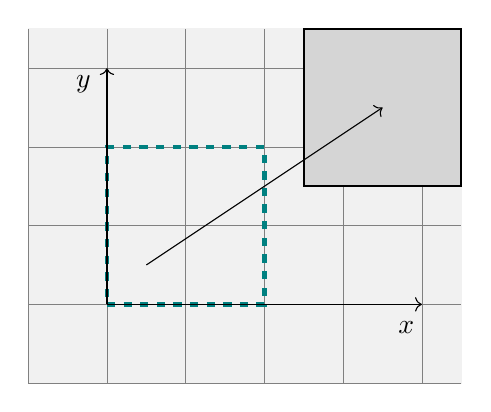
\begin{tikzpicture}
\draw[fill=gray!11,gray!11](0,0) rectangle (5.5,4.5);
\draw[step=1cm,gray,very thin] (0,0) grid (5.5,4.5); %background grid
\draw[ultra thick,dashed,teal] (1,1) -- (3,1) -- (3,3) -- (1,3) -- cycle;
\draw[thin,->]   (1,1) -- (5,1) ;
\draw[thin,->]   (1,1) -- (1,4) ;
\draw[fill=gray!33,thick] (3.5,2.5) -- (5.5,2.5) -- (5.5,4.5) -- (3.5,4.5) -- cycle; 
\node[] at (4.8,0.7) {$x$};
\node[] at (0.7,3.8) {$y$};
\draw[thin,->]   (1.5,1.5) -- (4.5,3.5) ;
\end{tikzpicture}
\end{center}

There is no deformation to speak of since the body remains the same but translated. 
The equation above also writes
\[
\left(
\begin{array}{c}
x \\ y
\end{array}
\right)
=
\underbrace{
\left(
\begin{array}{cc}
1 & 0 \\
0 & 1
\end{array}
\right)
}_{\bm F}
\cdot
\left(
\begin{array}{c}
X \\ Y
\end{array}
\right)
+
\left(
\begin{array}{c}
2.5 \\ 1.5
\end{array}
\right)
\]
We will see the significance of the matrix ${\bm F}$ in what follows.

\paragraph{Rigid body rotation} For instance:
\begin{eqnarray}
x &=& X \cos \theta - Y \sin \theta \\ 
y &=& X \sin \theta + Y \cos \theta 
\end{eqnarray}


\begin{center}
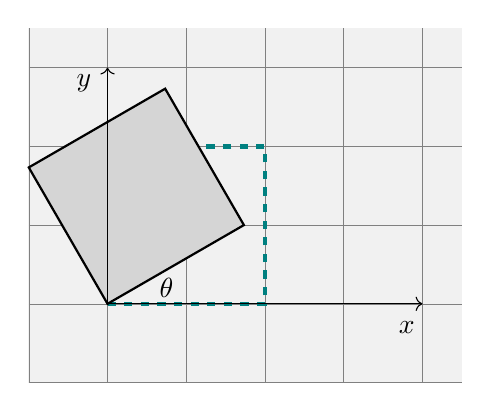
\begin{tikzpicture}
\draw[fill=gray!11,gray!11](0,0) rectangle (5.5,4.5);
\draw[step=1cm,gray,very thin] (0,0) grid (5.5,4.5); 
\draw[ultra thick,dashed,teal] (1,1) -- (3,1) -- (3,3) -- (1,3) -- cycle;
\draw[fill=gray!33,thick] (1,1) -- (2.732,2) -- (1.732,3.732) -- (0,2.732) -- cycle; 
\draw[thin,->]   (1,1) -- (5,1) ;
\draw[thin,->]   (1,1) -- (1,4) ;
\node[] at (4.8,0.7) {$x$};
\node[] at (0.7,3.8) {$y$};
\node[] at (1.75,1.2) {$\theta$};
\end{tikzpicture}
\end{center}


This can be rewritten as $\vec{x}={\bm F}\cdot \vec{X}$, where 
${\bm F}$ is a rotation matrix counter-clockwise about the $z$ axis (perpendicular
to the page):
\[
{\bm F} = 
\left(
\begin{array}{cc}
\cos\theta & -\sin\theta \\
\sin\theta & \cos\theta 
\end{array}
\right)
\]
Actually the body is not deformed, but simply rotated. There is no strain associated to this 
transformation. 


\paragraph{Stretching} Let us now turn to a 'real' deformation with shape change: stretching. 
For instance:

\begin{equation}
\begin{cases} 
x &=2X  \\ 
y &=1.5 Y 
\end{cases}
\qquad
\Leftrightarrow
\qquad
{\bm F} = 
\left(
\begin{array}{cc}
2 & 0 \\
0 & 1.5
\end{array}
\right)
\label{eq:stretching1}
\end{equation}

\begin{center}
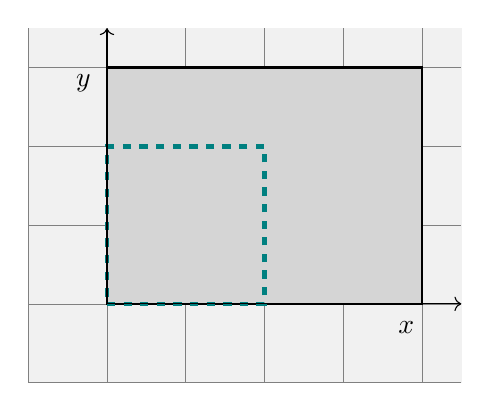
\begin{tikzpicture}
\draw[fill=gray!11,gray!11](0,0) rectangle (5.5,4.5);
\draw[step=1cm,gray,very thin] (0,0) grid (5.5,4.5); 
\draw[fill=gray!33,thick] (1,1) -- (5,1) -- (5,4) -- (1,4) -- cycle;
\draw[ultra thick,dashed,teal] (1,1) -- (3,1) -- (3,3) -- (1,3) -- cycle;
\draw[thin,->]   (1,1) -- (5.5,1) ;
\draw[thin,->]   (1,1) -- (1,4.5) ;
\node[] at (4.8,0.7) {$x$};
\node[] at (0.7,3.8) {$y$};
\end{tikzpicture}
\end{center}

This deformation has increased the area of the body by a factor 3.


\paragraph{Shearing} Another possible deformation (and a very relevant one 
in structural geology) is shearing:
\begin{equation}
\begin{cases} 
x &=X  \\ 
y &=\frac12 X + Y 
\end{cases}
\qquad
\Leftrightarrow
\qquad
{\bm F} = 
\left(
\begin{array}{cc}
1 & 0 \\
\frac12 & 1
\end{array}
\right)
\label{eq:shearing0}
\end{equation}



\begin{center}
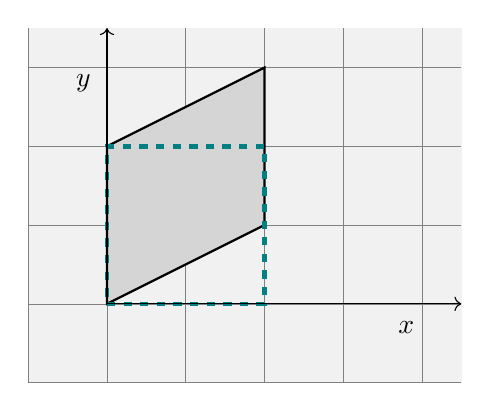
\begin{tikzpicture}
\draw[fill=gray!11,gray!11](0,0) rectangle (5.5,4.5);
\draw[step=1cm,gray,very thin] (0,0) grid (5.5,4.5); 
\draw[fill=gray!33,thick] (1,1) -- (3,2) -- (3,4) -- (1,3) -- cycle;
\draw[ultra thick,dashed,teal] (1,1) -- (3,1) -- (3,3) -- (1,3) -- cycle;
\draw[thin,->]   (1,1) -- (5.5,1) ;
\draw[thin,->]   (1,1) -- (1,4.5) ;
\node[] at (4.8,0.7) {$x$};
\node[] at (0.7,3.8) {$y$};
\end{tikzpicture}
\end{center}

This is a case of \underline{simple shear}: a deformation in which parallel planes in a material remain 
parallel and maintain a constant distance, while translating relative to each other. 
We see that the area of the body is conserved but not its shape.
\index{general}{Simple shear}


Let us now consider this shear example:

\begin{equation}
\begin{cases} 
x &=X + \frac12 Y \\ 
y &=\frac12 X + Y 
\end{cases}
\qquad
\Leftrightarrow
\qquad
{\bm F} = 
\left(
\begin{array}{cc}
1 & \frac12 \\
\frac12 & 1
\end{array}
\right)
\label{eq:shearing1}
\end{equation}

\begin{center}
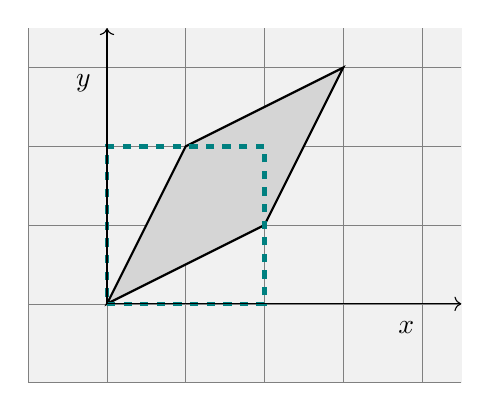
\begin{tikzpicture}
\draw[fill=gray!11,gray!11](0,0) rectangle (5.5,4.5);
\draw[step=1cm,gray,very thin] (0,0) grid (5.5,4.5); 
\draw[fill=gray!33,thick] (1,1) -- (3,2) -- (4,4) -- (2,3) -- cycle;
\draw[ultra thick,dashed,teal] (1,1) -- (3,1) -- (3,3) -- (1,3) -- cycle;
\draw[thin,->]   (1,1) -- (5.5,1) ;
\draw[thin,->]   (1,1) -- (1,4.5) ;
\node[] at (4.8,0.7) {$x$};
\node[] at (0.7,3.8) {$y$};
\end{tikzpicture}
\end{center}

Here too the shape changes and we obtain a parallelogram. However, 
the area is not conserved since the area of the undeformed square is 4, 
while the area of the parallelogram is 3
(Split it in two triangles. The area of the triangle inside the square is 4-1-1-0.5).

So while the expression for ${\bm F}$ above may superficially resemble 
pure shear (irrotational, area preserving shear), it is not. 
To describe pure shear with ${\bm F}$, the diagonal terms are no longer 1. 
The following shear example does describe pure shear:
\begin{equation}
\begin{cases} 
x &=1.25X + 0.75 Y \\ 
y &=0.75 X + 1.25Y 
\end{cases}
\qquad
\Leftrightarrow
\qquad
{\bm F} = 
\left(
\begin{array}{cc}
1.25 & 0.75 \\
0.75 & 1.25
\end{array}
\right)
=\frac14
\left(
\begin{array}{cc}
5 & 3 \\
3 & 5
\end{array}
\right)
\label{eq:shearing3}
\end{equation}

\begin{center}
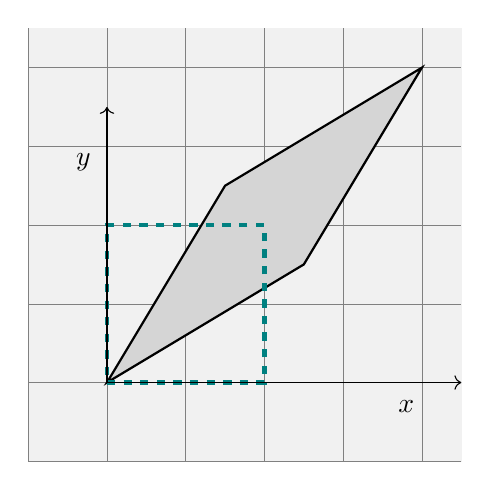
\begin{tikzpicture}
\draw[fill=gray!11,gray!11](0,0) rectangle (5.5,5.5);
\draw[step=1cm,gray,very thin] (0,0) grid (5.5,5.5); 
\draw[fill=gray!33,thick] (1,1) -- (3.5,2.5) -- (5,5) -- (2.5,3.5) -- cycle;
\draw[ultra thick,dashed,teal] (1,1) -- (3,1) -- (3,3) -- (1,3) -- cycle;
\draw[thin,->]   (1,1) -- (5.5,1) ;
\draw[thin,->]   (1,1) -- (1,4.5) ;
\node[] at (4.8,0.7) {$x$};
\node[] at (0.7,3.8) {$y$};
%\node[] at (1.75,1.2) {$\theta$};
\end{tikzpicture}
\end{center}

The area of the resulting parallelogram is still 1, so this deformation conserves volume.

 


%......................................................................
%\subsection*{Combination of deformations}

%So far we have then seen two types of deformation: stretching and shear, and these
%can also be accompanied by rotation. 
%It then makes sense to think of a deformed body as the result of successive 
%shearing, stretching and rotation. 


%\begin{center}
%\includegraphics[width=8cm]{python_codes/fieldstone_89/images/broerse}\\
%{\captionfont Taken from Broerse et al, subm.
%Any homogeneous deformation ${\bm F}$ can be written as a succession of a simple shear
%parallel to x called ${\bm \Gamma}$; an extension in x and an extension in y direction called
%${\bm \Lambda}$; followed by an orthogonal rotation ${\bm Q}$. 
%Here, the change between initial line vectors $d\vec{X}$ (in this case
%the side vectors of a square) to final initial line vectors $d\vec{x}$ (the deformed quadrilaterals) is
%determined by: $d\vec{x} = {\bm F} \cdot d\vec{X}$. 
%First row, incremental deformation, second row, cumulative deformation.
%}
%\end{center}


%Thinking of ${\bm F}$ as the matrix which transforms $\vec{X}$ into $\vec{x}$
%it then makes sense to decompose it into the product of three matrices, 
%one accounting for rotation ${\bm R}$ (or ${\bm Q}$ as in the example above), 
%one for stretching ${\bm \Lambda}$ and
%one for shearing ${\bm \Gamma}$.
%However, there is a caveat in this approach: it is easy to show that 
%these transformations do not necessarily commute, i.e. the order in which 
%these transformations are succesively applied matters.

%We then write
%\[
%{\bm F} = {\bm R} \cdot {\bm \Lambda} \cdot {\bm \Gamma}
%\] 

%......................................................................
\subsection*{Polar decomposition of ${\bm F}$}

A polar decomposition separates ${\bm F}$ into a rotation and a stretching of 
the space along a set of orthogonal axes\footnote{\url{https://en.wikipedia.org/wiki/Polar_decomposition}}. 
\index{general}{Polar Decomposition}

For instance, let us now consider the following transformation:
\begin{equation}
\begin{cases} 
x &= 1.3X-0.375Y\\ 
y &= 0.75X+0.65 Y
\end{cases}
\qquad
\Leftrightarrow
\qquad
{\bm F} = 
\left(
\begin{array}{cc}
1.3 & -0.375 \\
0.75 & 0.650
\end{array}
\right)
\end{equation}
It can be decomposed as 
\[
{\bm F} = {\bm R} \cdot {\bm U}
=
\left(
\begin{array}{cc}
0.866 & -0.5 \\
0.5 & 0.866
\end{array}
\right)
\cdot
\left(
\begin{array}{cc}
1.5 & 0 \\
0 & 0.75
\end{array}
\right)
\]
where ${\bm R}$ is the aforementioned rotation,  
${\bm U}$ is the right stretch tensor, or as \index{general}{Right stretch Tensor} 
\[
{\bm F} = {\bm V} \cdot {\bm R}
=
\left(
\begin{array}{cc}
1.313 & 0.325 \\
0.325 & 0.938 
\end{array}
\right)
\cdot
\left(
\begin{array}{cc}
0.866 & -0.5 \\
0.5 & 0.866
\end{array}
\right)
\]
where ${\bm V}$ is the left stretch tensor. \index{general}{Left stretch Tensor} 
We see that ${\bm U}\ne {\bm V}$ but it can 
easily be proven that 
\[
{\bm V} = {\bm R}\cdot{\bm U}\cdot {\bm R}^T
\qquad
\text{and}
\qquad
{\bm U} = {\bm R}^T\cdot{\bm V}\cdot {\bm R}
\]
Note that  ${\bm V}$ and ${\bm U}$ are symmetric, and have positive eigenvalues, and the 
eigenvalues correspond to stretches in $[0,\infty]$.
These stretches then form the axes of a strain ellipse. 
$U$ and $V$ have furthermore the same eigenvalues, but their eigenvectors are 
rotated with regards to each other since ${\bm U} = {\bm R}^T \cdot {\bm V} \cdot {\bm R}$ (which is basically a coordinate rotation).



\begin{center}
\includegraphics[width=8cm]{python_codes/fieldstone_89/images/polardec}\\
{\captionfont Taken from Broerse et al, subm. 
Sketch of the polar decomposition of the deformation gradient ${\bm F}$ into an orthogonal
rotation $R$ and symmetric stretch tensors $V$ or $U$. Here we apply the deformation of $F$ to an
initially square material element, with side vectors $d\vec{X}$. 
The deformed configuration (right)
leads to an element with side vectors $dx = FdX$. 
The decomposition can be written as first
a stretch $U$ followed by a rotation $R$, or first a rotation $R$ followed by a stretch $V$. 
Principal stretches $\vec\lambda$ of $V$ provide the stretch in the final, deformed, configuration, 
whereas stretches $\vec\lambda$ of $U$ provide the stretch in the original configuration. 
Material axes provide reference for the reader. 
We also show strain ellipses in black, that can be constructed using circle coordinates
as $dX$. Because $V$ and $U$ are symmetric tensors, the rotation angle of $R$ is non-zero for simple
shear contributions.}
\end{center}





\begin{itemize}
\item
The actual decomposition algorithm is not trivial, 
even for $2\times2$ matrices. This is nicely documented 
online\footnote{\url{http://www.continuummechanics.org/polardecomposition.html}}.
For instance, coming back to the simple shear example of Eq.~\eqref{eq:shearing0}, 
the tensor ${\bm F}$ can be written 
\[
{\bm F}= {\bm R} \cdot {\bm U}
=
\left(
\begin{array}{cc}
\cos\theta & -\sin\theta \\
\sin\theta & \cos\theta 
\end{array}
\right)
\cdot
\left(
\begin{array}{cc}
U_{xx} & U_{xy} \\
U_{yx} & U_{yy} 
\end{array}
\right)
\]
We must then determine $U_{ij}$ and $\theta$ which is, once again, not trivial. We then use the method 
of Hoger \& Carlson(1984) \cite{hoca84} (see note in a couple of pages further). We start by computing
\[
{\bm C} =
 {\bm F}^T\cdot{\bm F}
=
\left(
\begin{array}{cc}
1 & 1/2 \\ 
0 & 1
\end{array}
\right)
\cdot
\left(
\begin{array}{cc}
1 & 0 \\ 
1/2 & 1
\end{array}
\right)
=
\left(
\begin{array}{cc}
5/4 & 1/2 \\ 
1/2 & 1
\end{array}
\right)
\]
We then proceed by computing the 1st and 2nd invariants of ${\bm C}$:
\begin{eqnarray}
I_C &=&C_{xx}+C_{yy}=5/4+1=9/4 \nonumber\\
II_C&=&C_{xx}C_{yy}-C_{xy}C_{yx} = 5/4-1/4 = 1 \nonumber
\end{eqnarray}
and of ${\bm U}$
\begin{eqnarray}
I_U &=&\sqrt{I_C + 2 \sqrt{II_C}} = \sqrt{9/4 + 2 }= \frac{1}{2}\sqrt{17} \nonumber\\
II_U&=&\sqrt{II_C} = 1 \nonumber
\end{eqnarray}
Then the right stretch tensor is:
\[
{\bm U} = \frac{1}{I_U}({\bm C} + II_U {\bm I})
=
\frac{2}{\sqrt{17}}  \left[ 
\left(
\begin{array}{cc}
5/4 & 1/2 \\ 
1/2 & 1
\end{array}
\right)
+ 
\left(
\begin{array}{cc}
1 &0 \\ 0 & 1
\end{array}
\right)
\right]
=
\frac{2}{\sqrt{17}}  
\left(
\begin{array}{cc}
9/4 & 1/2 \\ 
1/2 & 2
\end{array}
\right)
\]
The inverse is simply:
\[
{\bm U}^{-1} 
=\frac{1}{U_{xx}U_{yy}-U_{xy}U_{yx}}
\left(
\begin{array}{cc}
U_{yy} & -U_{xy} \\
-U_{yx} & U_{xx} 
\end{array}
\right)
=
\frac{2}{\sqrt{17}}
\left(
\begin{array}{cc}
2 & -1/2 \\
-1/2 & 9/4
\end{array}
\right)
\]
Finally 
\[
{\bm R} = {\bm F} \cdot {\bm U}^{-1}
=
\left(
\begin{array}{cc}
1 & 0 \\
\frac12 & 1
\end{array}
\right)
\cdot
\frac{2}{\sqrt{17}}
\left(
\begin{array}{cc}
2 & -1/2 \\
-1/2 & 9/4
\end{array}
\right)
=
\frac{2}{\sqrt{17}}
\left(
\begin{array}{cc}
2 & -1/2 \\
1/2 & 2
\end{array}
\right)
\]
Finally 
\[
\theta = \arctan R_{yx}/R_{xx} = \arctan \frac14 \simeq 14^o
\]
This is very important since it means that simple shear deformation generates rotation! 

It is also worth noting that since $\theta=14^o$, then the rotation matrix is 
\[
{\bm R} 
=
\left(
\begin{array}{cc}
\cos\theta & -\sin\theta \\
\sin\theta & \cos\theta 
\end{array}
\right)
\simeq
\left(
\begin{array}{cc}
0.9701 &  -0.2425 \\
0.2425 & 0.9701 
\end{array}
\right)
\simeq
{\bm I} + 
\left(
\begin{array}{cc}
0 &  -0.2425 \\
0.2425 & 0 
\end{array}
\right)
\]


\item
Looking now at Eq.~\eqref{eq:shearing3}, then
\[
{\bm C} = {\bm F}^T\cdot{\bm F}
=
\frac{1}{8}
\left(
\begin{array}{cc}
17 & 15 \\
15 & 17
\end{array}
\right)
\]
We then proceed by computing the 1st and 2nd invariants of ${\bm C}$:
\begin{eqnarray}
I_C &=&C_{xx}+C_{yy} = 17/4\\
II_C&=&C_{xx}C_{yy}-C_{xy}C_{yx} = (17^2-15^2)/64 = 1
\end{eqnarray}
and of ${\bm U}$
\begin{eqnarray}
I_U &=&\sqrt{I_C + 2 \sqrt{II_C}} = \sqrt{ 17/4 + \sqrt{1}  } = \frac{5}{2}\\
II_U&=&\sqrt{II_C} = 1
\end{eqnarray}
Then the right stretch tensor is:
\[
{\bm U} = \frac{1}{I_U}({\bm C} + II_U {\bm I})
=
\frac{2}{5}
\frac{1}{8}
\left(
\begin{array}{cc}
17+8 & 15 \\
15 & 17+8
\end{array}
\right)
=
\frac{1}{4}
\left(
\begin{array}{cc}
5 & 3 \\
3 & 5
\end{array}
\right)
\]
Its inverse is 
\[
{\bm U}^{-1}
=
\frac{1}{4}
\left(
\begin{array}{cc}
5 & -3 \\
-3 & 5
\end{array}
\right)
\]
and finally 
\[
{\bm R}= {\bm F} \cdot {\bm U}^{-1}
=
\frac{1}{4}
\left(
\begin{array}{cc}
5 & 3 \\
3 & 5
\end{array}
\right)
\cdot
\frac{1}{4}
\left(
\begin{array}{cc}
5 & -3 \\
-3 & 5
\end{array}
\right)
={\bm I}
\]
This corresponds to an angle $\theta=0^o$, i.e. it is an irrotational deformation, and since
we have shown that it conserves volume, it is \underline{pure shear}.

Pure shear is an example of irrotational strain in which body is elongated in one direction 
while being shortened perpendicularly. Indeed, in this case we have extended the body 
along the (1,1) direction while squeezing it in the orthogonal (1,-1) direction.
Pure shear is differentiated from simple shear in that pure shear involves no rigid body rotation. 
\index{general}{Pure Shear}

\end{itemize}


\newpage
%%%%%%%%%%%%%%%%%%%%%%%%%%%%%%%%%%%%%%%%%%%%%%%%%%%%%%%%%%%%%%%%%%%%%%5
\subsection*{The deformation gradient}

There remains to formally define ${\bm F}$ as the deformation gradient.
\index{general}{Deformation Gradient}
It is defined as :
\[
\boxed{
{\bm F} = (\vec\nabla_X \vec{x})^T
= 
\left(\frac{\partial \vec{x}}{\partial \vec{X}} \right)^T
=
\left(
\begin{array}{cc}
\frac{\partial x}{\partial X} & 
\frac{\partial y}{\partial X} \\ \\
\frac{\partial x}{\partial Y} & 
\frac{\partial x}{\partial Y}  
\end{array}
\right)^T
=
\left(
\begin{array}{cc}
\frac{\partial x}{\partial X} & 
\frac{\partial x}{\partial Y} \\ \\
\frac{\partial y}{\partial X} & 
\frac{\partial x}{\partial Y}  
\end{array}
\right)
}
\]
The transpose is necessary and best explained through example. 
Looking at the first shearing example of Eq.~\eqref{eq:shearing1} again, we have

\begin{equation}
\begin{cases} 
x &=X  \\ 
y &=\frac12 X + Y 
\end{cases}
\qquad
\Leftrightarrow
\qquad
{\bm F} = 
\left(
\begin{array}{cc}
1 & 0 \\
\frac12 & 1
\end{array}
\right)
\label{eq:shearing2}
\end{equation}
and 
\[
\vec\nabla_{X}  \vec{x}=
\left(
\begin{array}{cc}
\frac{\partial x}{\partial X} & 
\frac{\partial y}{\partial X} \\ \\
\frac{\partial x}{\partial Y} & 
\frac{\partial x}{\partial Y}  
\end{array}
\right)
=
\left(
\begin{array}{cc}
1 & \frac12 \\ 
0 & 1
\end{array}
\right)
\]
which is indeed the transpose of ${\bm F}$.


We can write the displacement $\vec{u}$ as the difference between current and reference coordinates:
\[
\vec{u} = \vec{x}-\vec{X}
\]
and the deformation gradient can be reformulated as a function of the displacements:
\[
{\bm F} 
= \frac{\partial \vec{x}}{\partial \vec{X}} 
= \frac{\partial }{\partial \vec{X}} (\vec{X}+\vec{u})
= {\bm I} + \frac{\partial \vec{u}}{\partial \vec{X}} 
= {\bm I} + \vec{\nabla}\vec{u} 
\]
From this it follows that the infinitesimal strain tensor can be written
\[
\boxed{
{\bm \varepsilon}(\vec{u}) = \frac{1}{2}( \vec\nabla\vec{u} + \vec\nabla\vec{u}^T )
= \frac{1}{2} (  {\bm F} +  {\bm F}^T) - {\bm I} 
}
\]
and the rotation tensor is then 
\[
{\bm \omega} 
=\frac{1}{2}( \vec\nabla\vec{u} - \vec\nabla\vec{u}^T )
= \frac{1}{2} (  {\bm F} -  {\bm F}^T)
\]

\index{general}{Infinitesimal Strain Tensor}


%-------------------------------------------------------------
\subsection*{Purpose of this stone}

This stone has two purposes:
\begin{itemize}
\item put the theory above into practice 
\item show that the 'standard' way of integrating strain on Lagrangian markers in 
geodynamical codes is merely an approximation and that this approximation 
no longer holds for large deformations/rotations. In other words, 
integrated strain rates lose their physical meaning when 
the deformation becomes large!
\end{itemize}

In all what follows we denote by 'old' the method by which 
strain is accumulated onto markers by time integration of the strain rate components.
In practice here we interpolate $\vec\nabla \vec\upnu $ through $Q_1$ shape functions
in the middle of the Lagrangian grid cells, we compute $\dot{\varepsilon}_{ij}$, we
update the strain as $\varepsilon_{ij} += \dot{\varepsilon}_{ij} \delta t$.
As we will show, this is fine only for (very) small total strains. 

The 'new' method computes the marker strain by means 
of the deformation tensor.
For each cell centroid, we compute the displacement gradient tensor ${\bm F}$, 
then carry out polar decomposition to write ${\bm F}$ as product of stretch and rotation, 
i.e. ${\bm F}=  {\bm V}\cdot {\bm R}$.
From ${\bm V}$ we compute the principal stretches $\lambda_{1,2}$ (eigenvalues of ${\bm V}$) 
and the eigenvectors as well since these represent the axes of the strain ellipse, 
i.e. the directions of maximum stretch.
We then substract 1 to principal stretches to get principal strains, $\varepsilon_{1,2} = \lambda_{1,2}-1$.

The 'new' method (which is not that new since it is to be found in Malvern (1969) \cite{malvern} 
is as accurate as the measurement of ${\bm F}$ itself, and the difference tells us how bad 
the 'old' method actually can be (spoiler alert: up to few tens of \%).


%MOVE elsewhere:
%Also principal strains can never be smaller than -1 by def, because less than -1 means
%more than 100\%  shortening (in 1D). but no upper limit.
%conversely principal stretch > 0 (bc it is strain +1 ).


 

\newpage
%------------------------------------------------------------------------
\subsection*{Polar decomposition a la Hoger \& Carlson (1984)}

The polar decomposition of ${\bm F}$ is not trivial, but an 
application of the Cayley-Hamilton theorem allows for this 
as explained in Hoger \& Carlson (1984) \cite{hoca84}.

The deformation gradient tensor ${\bm F}$ is computed in the middle of
each cell at a given time $t$ as follows:
\[
{\bm F}(t)
=
\left(
\begin{array}{cc}
F_{xx} & F_{xy} \\
F_{yx} & F_{yy} 
\end{array}
\right)
=
{\bm I}+
\left(
\begin{array}{cc}
\frac{\partial (x(t)-x_0)}{\partial x}  & \frac{\partial (x(t)-x_0)}{\partial y}  \\
\frac{\partial (y(t)-y_0)}{\partial x}  & \frac{\partial (y(t)-y_0)}{\partial y}  
\end{array}
\right)
\]
In what follows we omit the time dependence '$(t)$'.
Each cell is assumed to be a $Q_1$ quadrilateral with a marker at each corner. We therefore store the 
initial position of markers, and make use of bilinear $Q_1$ shape functions to compute the derivatives
above in the center of the cell.

\begin{enumerate}
\item The right Cauchy-Green deformation tensor is defined as
\[
{\bm C} = {\bm F}^T {\bm F}
= ({\bm R}\cdot {\bm U})^T \cdot ({\bm R} \cdot {\bm U})
= {\bm U}^T \cdot {\bm R}^T \cdot {\bm R} \cdot {\bm U}
= {\bm U}^T \cdot {\bm U}
\]
\item 
We then find the eigenvalues of ${\bm C}$:
\[
\mu_{1,2} = \frac{1}{2}(C_{xx}+C_{yy}) \pm \sqrt{ \frac{1}{4}(C_{xx}-C_{yy})^2 + C_{xy}^2   }
\]
\item We compute the two invariants:
\[
I_C = \mu_1+\mu_2 \qquad II_C = \mu_1\mu_2 
\]
\item Compute invariants of right stretch tensor U
\[
I_U=\sqrt{I_C+2\sqrt{II_C}}
\qquad
II_U=\sqrt{II_C}
\]
\item compute right stretch tensor ${\bm U}$
\[
{\bm U} = \frac{{\bm C}+ II_U {\bm I}}{I_U}
\]
\item compute inverse of ${\bm U}$
\[
{\bm U}^{-1} = - I_U \frac{{\bm C}- (II_U+I_C){\bm I}}{II_U(II_U+I_C)+II_C}
\]
\item compute rotation matrix ${\bm R}={\bm F}{\bm U}^{-1}$

\item compute left stretch tensor ${\bm V}={\bm F}{\bm R}^T$

\item Compute eigenvalues of ${\bm V}$, which are the square roots of those of ${\bm C}$
\[
\lambda_1 = \sqrt{\mu_1}
\qquad
\lambda_2 = \sqrt{\mu_2}
\]

\end{enumerate}










\newpage
%%%%%%%%%%%%%%%%%%%%%%%%%%%%%%%%%%%%%%%%%%%%%%%%%%%%%%%%%%%%%%%%%%%%%%5
\subsection*{The shear band (experiment=1)}

The domain is a rectangle of size $L_x\times L_y$ discretised by nelx $\times$ nely $Q_2$ elements.
The following velocity field is precribed in the domain:
\begin{eqnarray}
u(x,y)&=&0 \\
v(x,y)&=&\text{erf} [A(x-L_x/2)]
\end{eqnarray}

A swarm of $41\times41$ markers is then placed in the domain, 
and they are then painted as shown here:
\begin{center}
\includegraphics[width=5.6cm]{python_codes/fieldstone_89/results/shearband/init/grid}
\includegraphics[width=5.6cm]{python_codes/fieldstone_89/results/shearband/init/vel}
\includegraphics[width=5.6cm]{python_codes/fieldstone_89/results/shearband/init/markers}\\
{\captionfont Domain is unit square, resolution $20\times20$ elements. $A=5$. 
Left: Eulerian grid; Middle: velocity field; Right: marker initial position.}
\end{center}

A time loop is implemented. At each time step the velocity field of the grid is 
interpolated onto each marker that is in turn advected with a simple euler step. 
\[
\vec{x}(t+\delta t) = \vec{x}(t) + \vec\upnu \; \delta t
\]
Note that the timestep value $\delta t$ is controlled by means of a CFL condition 
with ${\cal C}=0.1$. Likewise, the components of the strain rate tensor are computed on each marker and 
used to update the strain on each marker:
\[
\varepsilon_{ij}(t+\delta t) = \varepsilon_{ij}(t) + \dot\varepsilon_{ij}(t) \; \delta t
\]
These markers form a Lagrangian mesh which deforms over time:
\begin{center}
\includegraphics[width=6cm]{python_codes/fieldstone_89/results/shearband/init/swarm_mesh}
\includegraphics[width=6cm]{python_codes/fieldstone_89/results/shearband/init/swarm_paint}\\
{\captionfont Lagrangian mesh after 50 time steps.}
\end{center}
Markers which are advected outside of the domain are simply flagged inactive and these
are no longer advected. If one marker of a cell is flagged inactive so is the cell itself. 

At each time step the cumulative strain $\varepsilon_{ij}$ components are
computed at the center of the marker cells, as well as the principal strains $\varepsilon_1$ 
and $\varepsilon_2$ and the direction $\theta_\varepsilon$ of the principal strain:

\begin{center}
\includegraphics[width=6cm]{python_codes/fieldstone_89/results/shearband/old_angle_00}
\includegraphics[width=6cm]{python_codes/fieldstone_89/results/shearband/old_exy_00}\\
\includegraphics[width=6cm]{python_codes/fieldstone_89/results/shearband/old_angle_100}
\includegraphics[width=6cm]{python_codes/fieldstone_89/results/shearband/old_exy_100}\\
{\captionfont Left: principal strain directions, Right: $\varepsilon_{xy}$.
Top row: first time step; Bottom row: 100th time step.}
\end{center}


\begin{center}
\includegraphics[width=5cm]{python_codes/fieldstone_89/results/shearband/old_dirs0000}
\includegraphics[width=5cm]{python_codes/fieldstone_89/results/shearband/old_dirs0005}
\includegraphics[width=5cm]{python_codes/fieldstone_89/results/shearband/old_dirs0010}\\
\includegraphics[width=5cm]{python_codes/fieldstone_89/results/shearband/new_dirs0000}
\includegraphics[width=5cm]{python_codes/fieldstone_89/results/shearband/new_dirs0005}
\includegraphics[width=5cm]{python_codes/fieldstone_89/results/shearband/new_dirs0010}\\
{\captionfont Directions of the principal strains. Top is old (strain rate integration), 
bottom is new (finite strain). We see that 
the old method does not record any rotation and the angles remain at 45\si{\degree}. 
The new method shows principal strains which align more and more with the direction 
of shearing towards the center.}
\end{center}


A single cell is chosen in the middle of the domain and its strain values 
recorded over time in a file:
\begin{center}
\includegraphics[width=4cm]{python_codes/fieldstone_89/results/shearband/target0000.png}
\includegraphics[width=4cm]{python_codes/fieldstone_89/results/shearband/target0003.png}
\includegraphics[width=4cm]{python_codes/fieldstone_89/results/shearband/target0007.png}
\includegraphics[width=4cm]{python_codes/fieldstone_89/results/shearband/target0010.png}\\
{\captionfont Cell undergoing deformation.}
\end{center}

\begin{center}
\includegraphics[width=9.cm]{python_codes/fieldstone_89/results/shearband/principal_angle.pdf}
\includegraphics[width=9.cm]{python_codes/fieldstone_89/results/shearband/principal_strains.pdf}\\
\includegraphics[width=9.cm]{python_codes/fieldstone_89/results/shearband/area.pdf}
\includegraphics[width=9.cm]{python_codes/fieldstone_89/results/shearband/maximum_shear.pdf}\\
\includegraphics[width=9.cm]{python_codes/fieldstone_89/results/shearband/R.pdf}
\includegraphics[width=9.cm]{python_codes/fieldstone_89/results/shearband/V.pdf}\\
{\captionfont Time evolution of the principal angle $\theta_\varepsilon$, 
the strain principal values, the relative area change of the target cell, 
the components of ${\bm R}$, the components of ${\bm V}$ and the maximum 
possible shear.}
\end{center}










\newpage
%%%%%%%%%%%%%%%%%%%%%%%%%%%%%%%%%%%%%%%%%%%%%%%%%%%%%%%%%%%%%%%%%%%%%%5
\subsection*{The vertical extension (experiment=2)} 

In this case the velocity field is prescribed to be:
\begin{eqnarray}
u(x,y)&=&0 \\
v(x,y)&=&y
\end{eqnarray}
Since the divergence of this field is not zero, volume (area) is not conserved.

The components of the strain rate tensor are
\[
\dot\varepsilon_{xx} = 0 
\qquad
\dot\varepsilon_{yy} = 1
\qquad
\dot\varepsilon_{xy} = 0 
\]
So that the components of the strain for the old method are given by:
\[
\varepsilon_{xx} = 0 
\qquad
\varepsilon_{yy} = nstep \; \delta t
\qquad
\varepsilon_{xy} = 0 
\]



\begin{center}
\includegraphics[width=7cm]{python_codes/fieldstone_89/results/vertical/vel}\\
{\captionfont Velocity field on Eulerian mesh}
\end{center}


\begin{center}
\includegraphics[width=4cm]{python_codes/fieldstone_89/results/vertical/paint0000}
\includegraphics[width=4cm]{python_codes/fieldstone_89/results/vertical/paint0005}
\includegraphics[width=4cm]{python_codes/fieldstone_89/results/vertical/paint0010}
\includegraphics[width=4cm]{python_codes/fieldstone_89/results/vertical/paint0015}
\end{center}

\begin{center}
\includegraphics[width=4cm]{python_codes/fieldstone_89/results/vertical/target0000}
\includegraphics[width=4cm]{python_codes/fieldstone_89/results/vertical/target0005}
\includegraphics[width=4cm]{python_codes/fieldstone_89/results/vertical/target0010}
\includegraphics[width=4cm]{python_codes/fieldstone_89/results/vertical/target0015}\\
REDO
\end{center}

\begin{center}
\includegraphics[width=9.5cm]{python_codes/fieldstone_89/results/vertical/principal_angle.pdf}
\includegraphics[width=9.5cm]{python_codes/fieldstone_89/results/vertical/principal_strains.pdf}\\
\includegraphics[width=9.5cm]{python_codes/fieldstone_89/results/vertical/area.pdf}
\includegraphics[width=9.5cm]{python_codes/fieldstone_89/results/vertical/maximum_shear.pdf}\\
\includegraphics[width=9.5cm]{python_codes/fieldstone_89/results/vertical/R.pdf}
\includegraphics[width=9.5cm]{python_codes/fieldstone_89/results/vertical/V.pdf}\\
{\captionfont Time evolution of the principal angle $\theta_\varepsilon$, 
the strain principal values, the relative area change of the target cell, 
the components of ${\bm R}$, the components of ${\bm V}$ and the maximum
possible shear.}
\end{center}





\newpage
%%%%%%%%%%%%%%%%%%%%%%%%%%%%%%%%%%%%%%%%%%%%%%%%%%%%%%%%%%%%%%%%%%%%%%5
\subsection*{Pure shear (experiment=3)}

The velocity field is given by
\begin{eqnarray}
u(x,y)&=&x \nonumber\\
v(x,y)&=&y \nonumber
\end{eqnarray}
The components of the strain rate tensor are
\[
\dot\varepsilon_{xx} = 1 
\qquad
\dot\varepsilon_{yy} = 1
\qquad
\dot\varepsilon_{xy} = 0 
\]
So that the components of the strain for the old method are given by:




\begin{center}
\includegraphics[width=7cm]{python_codes/fieldstone_89/results/pureshear/vel}\\
{\captionfont Velocity field on Eulerian mesh}
\end{center}

\begin{center}
\includegraphics[width=4cm]{python_codes/fieldstone_89/results/pureshear/paint0000}
\includegraphics[width=4cm]{python_codes/fieldstone_89/results/pureshear/paint0005}
\includegraphics[width=4cm]{python_codes/fieldstone_89/results/pureshear/paint0010}\\
\includegraphics[width=4cm]{python_codes/fieldstone_89/results/pureshear/old_dirs0000}
\includegraphics[width=4cm]{python_codes/fieldstone_89/results/pureshear/old_dirs0005}
\includegraphics[width=4cm]{python_codes/fieldstone_89/results/pureshear/old_dirs0010}\\
{\captionfont old and new are identical}
\end{center}

\begin{center}
\includegraphics[width=3cm]{python_codes/fieldstone_89/results/pureshear/target0000}
\includegraphics[width=3cm]{python_codes/fieldstone_89/results/pureshear/target0005}
\includegraphics[width=3cm]{python_codes/fieldstone_89/results/pureshear/target0010}
\end{center}


\begin{center}
\includegraphics[width=9.5cm]{python_codes/fieldstone_89/results/pureshear/principal_angle.pdf}
\includegraphics[width=9.5cm]{python_codes/fieldstone_89/results/pureshear/principal_strains.pdf}\\
\includegraphics[width=9.5cm]{python_codes/fieldstone_89/results/pureshear/area.pdf}
\includegraphics[width=9.5cm]{python_codes/fieldstone_89/results/pureshear/maximum_shear.pdf}\\
\includegraphics[width=9.5cm]{python_codes/fieldstone_89/results/pureshear/R.pdf}
\includegraphics[width=9.5cm]{python_codes/fieldstone_89/results/pureshear/V.pdf}\\
{\captionfont Time evolution of the principal angle $\theta_\varepsilon$, 
the strain principal values, the relative area change of the target cell, 
the components of ${\bm R}$, the components of ${\bm V}$ and the maximum
possible shear.}
\end{center}

\newpage
%%%%%%%%%%%%%%%%%%%%%%%%%%%%%%%%%%%%%%%%%%%%%%%%%%%%%%%%%%%%%%%%%%%%%%5
\subsection*{Bi-axial stretch (experiment=4)}

The velocity is given by
\begin{eqnarray}
u(x,y)&=&-x+L_x/2 \\
v(x,y)&=&y-L_y/2
\end{eqnarray}
The components of the strain rate tensor are
\[
\dot\varepsilon_{xx} = -1 
\qquad
\dot\varepsilon_{yy} = 1
\qquad
\dot\varepsilon_{xy} = 0 
\]
The velocity divergence is zero. The components of the strain for the old method are given by:




\begin{center}
\includegraphics[width=7cm]{python_codes/fieldstone_89/results/biaxial/vel}\\
{\captionfont Velocity field on Eulerian mesh}
\end{center}


\begin{center}
\includegraphics[width=4cm]{python_codes/fieldstone_89/results/biaxial/target0000}
\includegraphics[width=4cm]{python_codes/fieldstone_89/results/biaxial/target0005}
\includegraphics[width=4cm]{python_codes/fieldstone_89/results/biaxial/target0010}
\end{center}

\begin{center}
\includegraphics[width=4cm]{python_codes/fieldstone_89/results/biaxial/paint0000}
\includegraphics[width=4cm]{python_codes/fieldstone_89/results/biaxial/paint0005}
\includegraphics[width=4cm]{python_codes/fieldstone_89/results/biaxial/paint0010}
\includegraphics[width=4cm]{python_codes/fieldstone_89/results/biaxial/paint0015}
\end{center}

\begin{center}
\includegraphics[width=4cm]{python_codes/fieldstone_89/results/biaxial/new_dirs0000}
\includegraphics[width=4cm]{python_codes/fieldstone_89/results/biaxial/new_dirs0005}
\includegraphics[width=4cm]{python_codes/fieldstone_89/results/biaxial/new_dirs0010}
\includegraphics[width=4cm]{python_codes/fieldstone_89/results/biaxial/new_dirs0015}
\end{center}

\begin{center}
\includegraphics[width=9.cm]{python_codes/fieldstone_89/results/biaxial/principal_angle.pdf}
\includegraphics[width=9.cm]{python_codes/fieldstone_89/results/biaxial/principal_strains.pdf}\\
\includegraphics[width=9.cm]{python_codes/fieldstone_89/results/biaxial/area.pdf}
\includegraphics[width=9.cm]{python_codes/fieldstone_89/results/biaxial/maximum_shear.pdf}\\
\includegraphics[width=9.cm]{python_codes/fieldstone_89/results/biaxial/R.pdf}
\includegraphics[width=9.cm]{python_codes/fieldstone_89/results/biaxial/V.pdf}\\
{\captionfont Time evolution of the principal angle $\theta_\varepsilon$, 
the strain principal values and the area of the target cell.}
\end{center}

PB: e2 cannot become less than -1 


\subsection*{Discussion 'old' vs. 'new' cumulative strain}

The first observation is that all quantities from the 'old' (integrated strain rates) and 'new' 
(strain computed from cumulative displacements) start at the same values. 
The 'old' cumulative strains are thus an acceptable approximation for small deformations. 
For increasing deformation a number of problems arise with the 'old' strains:

\begin{itemize}
\item principal axes do not rotate for simple shear (The shear band, experiment 1) while they should continuously change
\item principal strain values deviate from the exact values (the 'new' principal strains) (all experiments)
\item negative principal strains for the 'old' definition can decrease below the theoretical limit of -1 (The shear band, experiment 1; bi-axial stretch, experiment 4)
\item related to the previous point, the area computed from these principal strains may incorrectly become negative (The shear band, experiment 1;  bi-axial stretch, experiment 4)
\item the maximum shear deviates from the correct value (all experiments except for experiment 1)
\end{itemize}

The problems in the integration of strain rates is due to two causes. Firstly, strain rates are determined relative to the current state (already deformed), which means that the state with respect the deformation is defined changes during integration. Rather, the 'new' strains based on the cumulative  displacements are all references with respect to the original, undeformed, configuration. Secondly, because incremental principal axes change during general deformation that contains simple shear or rigid body rotation (which does not occur for the special cases of experiment 2, 3 and 4), incremental strains cannot be summed \cite{malvern}. In the special cases where there is no rotation, strain rates may be integrated, and the result is a strain measure called natural strain or Hencky strain \cite{malvern}.


\Literature: \textcite{mcke79} (1979), \textcite{mcja83} (1983), \textcite{foti93} (1993), \textcite{tifo93} (1993) 

 %%%%%%%%%%%%%%%%%%%%%%%%%%%%%%%%%%%%%%%%%%%%%%%%%%%%%%%%%%%%%%%%%%%%%

\chapter{Thick-walled elastic cylinder under uniform boundary pressure \label{f90}} %%%%%%%%%%%%%%%%%%%%%%%%% 90
\lstinputlisting[language=bash,basicstyle=\small]{python_codes/fieldstone_90/keywords.ascii}

\begin{center}
Code at \url{https://github.com/cedrict/fieldstone/tree/master/python_codes/fieldstone_90}
\end{center}

\par\noindent\rule{\textwidth}{0.4pt}

This axisymmetric elastic probem is common in the literature, see for instance Sadd \cite{sadd14}.
A hollow thick-walled cylinder is placed under the
action of uniform internal and external pressure loadings, as shown here:

\begin{center}
\includegraphics[width=4cm]{python_codes/fieldstone_90/images/sadda}\\
{\captionfont Taken from Sadd \cite{sadd14}}
\end{center}
One can easily show that the stress components are such that
\begin{eqnarray}
\sigma_{rr} &=& \frac{A}{r^2} + B \\
\sigma_{\theta\theta} &=& -\frac{A}{r^2} + B
\end{eqnarray}

Applying the boundary conditions 
$\sigma_r(r_1)=-p_1$ and $\sigma_r=-p_2$ 
creates two equations
for the two unknown constants $A$ and $B$. 
Solving for these constants gives the result
\begin{eqnarray}
A &=& \frac{r_1^2r_2^2(p_2-p_1)}{r_2^2-r_1^2} \\
B &=& \frac{r_1^2p_1-r_2^2p_2 )}{r_2^2-r_1^2} 
\end{eqnarray}
Substituting these values back into relations above gives the final result for the stress field.

Taking $r_1=0.5$, $r_2=1$, $p_2=0$ and $p_1=p$, we can plot these:
\begin{center}
\includegraphics[width=5cm]{python_codes/fieldstone_90/images/saddb}\\
{\captionfont Taken from Sadd \cite{sadd14}}
\end{center}

Using the strain-displacement relations and Hooke's law, the radial
displacement is easily determined as
\[
u_r = \frac{1+\nu}{E}r \left[ (1-2\nu) B - \frac{A}{r^2}\right]
\]
Looking at the solution, we see that 
the stress field does not depend on the elastic constants, although the
resulting displacements do depend on both $E$ and $\nu$.
\begin{eqnarray}
\varepsilon_{rr} &=& \frac{\partial u_r}{\partial r} = 
\frac{1+\nu}{E} \left[ (1-2\nu) B + \frac{A}{r^2}\right]
\\
\varepsilon_{\theta\theta} &=& \frac1r \frac{\partial u_\theta}{\partial \theta} + \frac{u_r}{r} 
=\frac{u_r}{r}  
=\frac{1+\nu}{E} \left[ (1-2\nu) B - \frac{A}{r^2}\right] 
\\
\varepsilon_{zz} &=& \frac{\partial u_z}{\partial z} = 0 
\end{eqnarray}
It then follows that 
\[
\sigma_{zz} = \lambda div(\vec{u}) + 2 \mu \varepsilon_{zz} = \lambda (\varepsilon_{rr} + \varepsilon_{\theta\theta})
\qquad
\text{and}
\qquad
\sigma_{rz} = 2 \mu \varepsilon_{rz} 
\]

We approach this problem by assuming that the cylinder is infinite in the direction perpendicular 
to the page. We have an obvious axisymmetry: 

\begin{center}
\includegraphics[width=4cm]{python_codes/fieldstone_90/images/cyl}
\includegraphics[width=7cm]{python_codes/fieldstone_90/images/cyl2}\\
\end{center}

The setup is then as follows:

\begin{center}
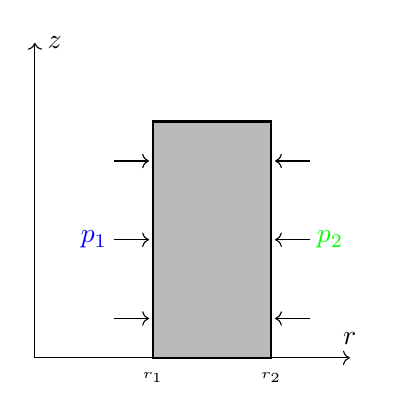
\begin{tikzpicture}
%\draw[fill=gray!23,gray!23](0,0) rectangle (6,5);
%\draw[step=0.5cm,gray,very thin] (0,0) grid (6,5); %background grid
\draw[thick,fill=gray!54] (2.5,.5)--(4,.5)--(4,3.5)--(2.5,3.5) -- cycle;

\draw[thin,->] (1,0.5) -- (5,0.5); %x
\draw[thin,->] (1,0.5) -- (1,4.5); %y
\node[] at (5,0.75) {$r$};
\node[] at (1.25,4.5) {$z$};

\node[] at (2.5,0.25) {\tiny $r_1$};
\node[] at (4,0.25) {\tiny $r_2$};

\draw[thin,->] (2,1) -- (2.45,1);
\draw[thin,->] (2,2) -- (2.45,2);
\draw[thin,->] (2,3) -- (2.45,3);

\draw[thin,->] (4.5,1) -- (4.05,1);
\draw[thin,->] (4.5,2) -- (4.05,2);
\draw[thin,->] (4.5,3) -- (4.05,3);

\node[] at (1.75,2) {\color{blue} $p_1$};
\node[] at (4.75,2) {\color{green} $p_2$};
\end{tikzpicture}
\end{center}

Because we have the analytical displacement field, we will be using it to 
impose Dirichlet boundary conditions on the sides, rather than pressure, and 
we will then recover strain and stress components.

Results for displacement, strain and stress as a function of $r$ are shown hereunder:
\begin{center}
\includegraphics[width=5.4cm]{python_codes/fieldstone_90/results/displacement.pdf}
\includegraphics[width=5.4cm]{python_codes/fieldstone_90/results/strain.pdf}
\includegraphics[width=5.4cm]{python_codes/fieldstone_90/results/stress.pdf}
\end{center}
The match is perfect and shows that the axisymmetric formulation presented in Section~\ref{ss:fem_elast_axis} is correct.

 %%%%%%%%%%%%%%%%%%%%%%%%%%%%%%%%%%%%%%%%%%%%%%%%%%%%%%%%%%%%%%%%%%%%%

\chapter{Stokes sphere in a cylinder, axisymmetric formulation ($Q_2\times Q_1$) \label{f91}} %%%%%%%%%%%%%%% 91
\lstinputlisting[language=bash,basicstyle=\small]{python_codes/fieldstone_91/keywords.ascii}

\begin{center}
Code at \url{https://github.com/cedrict/fieldstone/tree/master/python_codes/fieldstone_91}
\end{center}

\par\noindent\rule{\textwidth}{0.4pt}

%%%%%%%%%%%%%%%%%%%%%%%%%%%%%%%%%%%%%%%%%%%%%%%%%%%%%%%%%%%%%%%%%%%%%%%%%%%%%%%%%%%%%%%%%%%%%%%%%%%%


This stone carries out the Stokes sphere benchmark of Section~\ref{ss:stokes_sphere3D} although 
it uses an axisymmetric formulation, so that the sphere is actually falling inside 
a vertical cylinder. As a consequence, the boundary conditions are: 
free slip on the left (the axis of symmetry), top and bottom, and no slip on the right (the
wall of the cylinder). The default domain size is $L_r=0.5$ and $L_z=1$.

Having established the weak form of the Stokes equations and discretised them in 
Section~\ref{ss:cyl_axi}, transforming a 2D plane-strain code into an axisymmetric one is rather straightforward.
In a nutshell, 
\begin{itemize}
\item $x$ stands for r
\item $\upnu_r$ is $u$, $\upnu_z$ is $w$
\item the matrix ${\bm B}$ goes from 
$3 \times m_v\cdot ndofV$ to $4 \times m_v\cdot ndofV$. 
\item the matrix ${\bm N}$ goes from $3 \times m_p\cdot ndofP$ to $4 \times m_p\cdot ndofP$. 
\item the matrix ${\bm C}$ goes from $3 \times 3$ to $4 \times 4$.
\item integrals must be multiplied by $2 \pi$ and also contain an additional $r$ term
which translates into $x_q$ in the code. 
\end{itemize}

The Stokes sphere velocity is given by
\[
\upnu_{Stokes} = \frac{2}{9} \frac{\delta \rho}{\eta_f} R_s^2 g
\]
which yields $\upnu_S\simeq 3.387 \cdot 10^{-5}$. However, 
this is for a sphere in an infinite domain. When placed in a 
cylinder, the influence of the walls will slow the sphere down. 
Two corrections have been proposed be Habermann and by Faxen.

We start by writing the drag force
\[
F_H = 6 \pi \eta_f R \upnu_{sphere}\;  \gamma\left(\frac{r}{R}\right) 
\]
In the case of the Stokes sphere in an infinite medium then $\gamma =1$ and equating
$F_H$ with the buoyancy force $4/3 \pi R^3 \delta\rho g$ yields the above velocity.
Habermann gives a coefficient $\gamma$ such that 
\[
\gamma\left(\frac{r}{R}\right)  = \frac{1-0.75857 \left(\frac{r}{R}\right)^5}{1+f_H\left(\frac{r}{R}\right)}
\]
with 
\[
f_H\left(\frac{r}{R}\right) = -2.1050\left(\frac{r}{R}\right)+ 2.0865\left(\frac{r}{R}\right)^3
- 1.7068\left(\frac{r}{R}\right)^5 + 0.72603\left(\frac{r}{R}\right)^6 
\]
Faxen gives a coefficient $\gamma$ such that 
\[
\gamma\left(\frac{r}{R}\right) = \frac{1}{1 + f_F\left(\frac{r}{R}\right)} 
\]
with 
\[
f_F\left(\frac{r}{R}\right) 
= -2.10444(\frac{r}{R}) 
+ 2.08877(\frac{r}{R})^3 
- 0.94813(\frac{r}{R})^5 
- 1.372(\frac{r}{R})^6 
+ 3.87(\frac{r}{R})^8 
- 4.19(\frac{r}{R})^{10}
\]
In all three cases we have 
\[
\upnu_{sphere} = \frac{2}{9} \frac{\delta \rho}{\eta_f} R_s^2 g \frac{1}{\gamma(\frac{r}{R})}
\]
Note that the Habermann \& Faxen expressions are copy-pasted from the GALE manual and 
are extremely comparable in value. I did not verify these yet. 
Please check Lindgren (1999) \cite{lind99} to do so. They are about half the value of the Stokes velocity
in this case. The three velocity values are computed directly in the code and exported alongside
the measured velocity.

We see that increasing the height of the cylinder does not substantially alter the results, and that 
the velocity in the middle of the sphere seems to converge to the expected ones:
\begin{center}
\includegraphics[width=5cm]{python_codes/fieldstone_91/results/vc.pdf}
\includegraphics[width=5cm]{python_codes/fieldstone_91/results/vrms.pdf}
\includegraphics[width=5cm]{python_codes/fieldstone_91/results/mass.pdf}\\
{\captionfont up to 256x512 elements!}
\end{center}


\begin{center}
\includegraphics[width=4cm]{python_codes/fieldstone_91/results/ps/vel}
\includegraphics[width=4cm]{python_codes/fieldstone_91/results/ps/press}
\includegraphics[width=4cm]{python_codes/fieldstone_91/results/ps/exx}
\includegraphics[width=4cm]{python_codes/fieldstone_91/results/ps/exy}\\
\includegraphics[width=4cm]{python_codes/fieldstone_91/results/axi/vel}
\includegraphics[width=4cm]{python_codes/fieldstone_91/results/axi/press}
\includegraphics[width=4cm]{python_codes/fieldstone_91/results/axi/exx}
\includegraphics[width=4cm]{python_codes/fieldstone_91/results/axi/exy}\\
{\captionfont Top row: plane strain; Bottom row: axisymmetric. Resolution 50x100}
\end{center}


 %%%%%%%%%%%%%%%%%%%%%%%%%%%%%%%%%%%%%%%%%%%%%%%%%%%%%%%%%%%%%%%%%%%%%

\chapter{Stokes sphere in a cylinder, axisymmetric formulation, $P_2^+\times P_{-1}$ \label{f92}} %%%%%%%%%%% 92
\lstinputlisting[language=bash,basicstyle=\small]{python_codes/fieldstone_92/keywords.ascii}

\begin{center}
Code at \url{https://github.com/cedrict/fieldstone/tree/master/python_codes/fieldstone_92}
\end{center}

\par\noindent\rule{\textwidth}{0.4pt}

%%%%%%%%%%%%%%%%%%%%%%%%%%%%%%%%%%%%%%%%%%%%%%%%%%%%%%%%%%%%%%%%%%%%%%%%%%%%%%%%%%%%%%%%%%%%%%%%%%%%


This stone solves the axisymmetric problem of the Stokes sphere in a cylinder, 
similarly to Stone 91. However, it relies on an unstructured grid with 
Crouzeix-Raviart elements (see Section~\ref{ss:XXX}).

The workflow is as follows: the main parameters are defined in {\sl parameters.py}.
The file {\sl generate\_nodes.py} uses these parameters to generate points on the 
boundary of the rectangular domain and on the half circle. 
A call to {\sl triangle} is then made and a very important additional parameter is passed
as argument to triangle: the maximum area of a triangle. 
{\sl triangle} returns the (constrained) Delaunay triangulation of these points, 
and this information is then read in by {\sl stone.py} which solves the 
Stokes equation in axisymmetric formulation (see Section~\ref{ss:XXX}). 
Boundary conditions are free slip everywhere except no slip on the right. 

All these actions are carried out automatically when the following script is 
used\footnote{It assumes that the triangle program has been compiled and 
is located outside of the fieldstone tree.}:
\begin{lstlisting}
python3 generate_nodes.py
cat mypoints mysegments > mesh.poly
../../../../triangle/triangle  -j -q -a0.00100 -o2 -pc mesh.poly
echo "nel="
head -1 mesh.1.ele 
head -1 mesh.1.ele > temp
echo "NV0="
head -1 mesh.1.node 
head -1 mesh.1.node >> temp
python3 stone.py
\end{lstlisting}

Two remarks: the code stems from another code which implemented time stepping, 
which explains there is now a single fake time step loop in it. 
Pressure normalisation is not done the right way: the pressure nullspace is 
not removed from the matrix, but the solution is later normalised so that 
its average over the domain is zero.

\begin{center}
\includegraphics[width=4.3cm]{python_codes/fieldstone_92/results/mesh1}
\includegraphics[width=4.3cm]{python_codes/fieldstone_92/results/mesh2}
\includegraphics[width=4.3cm]{python_codes/fieldstone_92/results/mesh3}
\includegraphics[width=4.3cm]{python_codes/fieldstone_92/results/mesh4}\\
{\captionfont Left to right: nel=2432,2468,2588,2866}
\end{center}


\begin{center}
\includegraphics[width=5.5cm]{python_codes/fieldstone_92/results/mat}
\includegraphics[width=5.5cm]{python_codes/fieldstone_92/results/area}
\includegraphics[width=5.5cm]{python_codes/fieldstone_92/results/vel}\\
\includegraphics[width=5.5cm]{python_codes/fieldstone_92/results/u}
\includegraphics[width=5.5cm]{python_codes/fieldstone_92/results/v}
\includegraphics[width=5.5cm]{python_codes/fieldstone_92/results/press}\\
\includegraphics[width=5.5cm]{python_codes/fieldstone_92/results/sr}
\includegraphics[width=5.5cm]{python_codes/fieldstone_92/results/tauxx}
\includegraphics[width=5.5cm]{python_codes/fieldstone_92/results/tauxy}
\end{center}

Because the triangle size varies a lot within a mesh, defining a mesh size $h$
makes littel sense, so we plot the following results as a function of the 
number of elements:

\begin{center}
\includegraphics[width=8cm]{python_codes/fieldstone_92/results/vrms}
\includegraphics[width=8cm]{python_codes/fieldstone_92/results/vc}\\
{\captionfont Left: vrms over the whole domain for $L_y=1$; Right: 
measured velocity in the middle of the sphere. Some weird 
effect is taking place at very high resolution...}
\end{center}

The parameter $n_p$ is user defined and is an attempt to parameterise 
the resolution of the domain sides and the half circle with a single parameter.
In {\sl parameters.py} we have:
\begin{lstlisting}
np_top=n_p
np_bottom=n_p
np_left=10*n_p
np_right=5*n_p
np_sphere=10*n_p
\end{lstlisting}

We see that the sphere velocity in its middle 
matches the Habermann and Faxen values remarkably well, 
especially when the domain is made taller (top and bottom 
boundaries are further away) and the viscosity of the 
sphere is brought up to $10^5$.


\begin{center}
\includegraphics[width=8cm]{python_codes/fieldstone_92/results/stress.png}
\includegraphics[width=8cm]{python_codes/fieldstone_92/results/theta.png}\\
{\captionfont Deviatoric stress principal directions (left) and angle (right).} 
\end{center}
 %%%%%%%%%%%%%%%%%%%%%%%%%%%%%%%%%%%%%%%%%%%%%%%%%%%%%%%%%%%%%%%%%%%%%

\chapter{Buoyancy-driven flow with ($P_2^+\times P_{-1}$) \label{f93}} %%%%%%%%%%%%%%%%%%%%%%%%%%%%%%%%%%%%%% 93
\lstinputlisting[language=bash,basicstyle=\small]{python_codes/fieldstone_93/keywords.ascii}

\begin{center}
Code at \url{https://github.com/cedrict/fieldstone/tree/master/python_codes/fieldstone_93}
\end{center}

\par\noindent\rule{\textwidth}{0.4pt}

%%%%%%%%%%%%%%%%%%%%%%%%%%%%%%%%%%%%%%%%%%%%%%%%%%%%%%%%%%%%%%%%%%%%%%%%%%%%%%%%%%%%%%%%%%%%%%%%%%%%


This stone solves the problem of buoyancy-driven flows generated 
by objects sinking in a fluid, potentially under a deformable free surface.
It relies on an unstructured grid with Crouzeix-Raviart elements 
(see Section~\ref{MMM-sec:crouzeix-raviart}).

The workflow is as follows: the main parameters are defined in {\sl parameters.py}.
The file {\sl generate\_nodes.py} uses these parameters to generate points on the 
boundary of the rectangular domain, on the surface and on the circle and its center. 
A call to {\sl triangle} is then made and a very important additional parameter is passed
as argument to triangle: the maximum area of a triangle. 
{\sl triangle} returns the (constrained) Delaunay triangulation of these points, 
and this information is then read in by {\sl stone.py} which solves the 
Stokes equation. 
Boundary conditions are free slip everywhere. This benchmark is described in 
Section~\ref{MMM-ss:stokes_sphere_fs2D}.

All these actions are carried out automatically when the following script is 
used\footnote{It assumes that the triangle program has been compiled and 
is located outside of the fieldstone tree.}:
\begin{lstlisting}
python3 generate_nodes.py
cat mypoints mysegments > mesh.poly
../../../../triangle/triangle  -j -q -a0.00100 -o2 -pc mesh.poly
echo "nel="
head -1 mesh.1.ele 
head -1 mesh.1.ele > temp
echo "NV0="
head -1 mesh.1.node 
head -1 mesh.1.node >> temp
python3 stone.py
\end{lstlisting}


Note that ressure normalisation is not done the right way: the pressure nullspace is 
not removed from the matrix, but the solution is later normalised at the top
of the domain or over the whole domain.

Time stepping is carried out and the time step $\delta t$ is computed with a CFL criterion.
Nodes are advected with their velocity but no remeshing is implemented so that when the 
deformation becomes to large around the sphere the triangles become really deformed and 
the simulation must be stopped. Given the parameters of this benchmark this corresponds 
to $t\simeq 30$, while the simulation should ideally have been run up to $t>100$.

\newpage
%....................................................
\paragraph{The Stokes sphere in a unit square}
The setup and all results are described in Section~\ref{MMM-ss:stokes_sphere2D}.
Nodes are added on a vertical line to facilitate pressure and velocity profile measurements.

\begin{center}
\includegraphics[width=7cm]{python_codes/fieldstone_93/results_exp1/grid}
\includegraphics[width=7cm]{python_codes/fieldstone_93/results_exp1/vel}\\
\includegraphics[width=7cm]{python_codes/fieldstone_93/results_exp1/press}
\includegraphics[width=7cm]{python_codes/fieldstone_93/results_exp1/sr}\\
{\captionfont  Mesh obtained with -a0.00050 in script, np=32. No-slip boundary conditions.}
\end{center}

\begin{center}
\includegraphics[width=5.7cm]{python_codes/fieldstone_93/results_exp1/u}
\includegraphics[width=5.7cm]{python_codes/fieldstone_93/results_exp1/v}
\includegraphics[width=5.7cm]{python_codes/fieldstone_93/results_exp1/pressure}\\
{\captionfont  Mesh obtained with -a0.00050 in script, np=24,32,48. No-slip boundary conditions.}
\end{center}

\newpage
%..........................................................
\paragraph{The Stokes sphere under a deformable surface}

Nodes on the deformable surface are flagged at the beginning of the calculations and 
exported to an ascii file for later postprocessing. The multiple measurements for this 
benchmark are thoroughly described and plotted in Section~\ref{MMM-ss:stokes_sphere_fs2D}.

\begin{center}
\includegraphics[width=6.5cm]{python_codes/fieldstone_93/50/mesh0000}
\includegraphics[width=6.5cm]{python_codes/fieldstone_93/50/mesh0136}\\
\includegraphics[width=5.5cm]{python_codes/fieldstone_93/50/meshzoom0000}
\includegraphics[width=5.5cm]{python_codes/fieldstone_93/50/meshzoom0136}\\
{\captionfont  Mesh obtained with -a0.00050 in script}
\end{center}

\begin{center}
\includegraphics[width=5.5cm]{python_codes/fieldstone_93/results_exp2/mesh1}
\includegraphics[width=5.5cm]{python_codes/fieldstone_93/results_exp2/mesh2}
\includegraphics[width=5.5cm]{python_codes/fieldstone_93/results_exp2/mesh3}\\
{\captionfont  Mesh obtained with -a0.00050, -a0.00025 and -a0.00005 in script}
\end{center}

\begin{center}
\includegraphics[width=4cm]{python_codes/fieldstone_93/results_exp2/vel_0000}
\includegraphics[width=4cm]{python_codes/fieldstone_93/results_exp2/p_0000}
\includegraphics[width=4cm]{python_codes/fieldstone_93/results_exp2/sr_0000}
\includegraphics[width=4cm]{python_codes/fieldstone_93/results_exp2/mat_0000}\\
\includegraphics[width=4cm]{python_codes/fieldstone_93/results_exp2/vel_0136}
\includegraphics[width=4cm]{python_codes/fieldstone_93/results_exp2/p_0136}
\includegraphics[width=4cm]{python_codes/fieldstone_93/results_exp2/sr_0136}
\includegraphics[width=4cm]{python_codes/fieldstone_93/results_exp2/mat_0136}\\
{\captionfont  Mesh obtained with -a0.00025 in script. Top row $t=0$, 
bottom row $t\simeq 30$.}
\end{center}


\newpage

\begin{center}
\includegraphics[width=5.7cm]{python_codes/fieldstone_93/results_exp2/vrms}
\includegraphics[width=5.7cm]{python_codes/fieldstone_93/results_exp2/vrms_sphere}
\includegraphics[width=5.7cm]{python_codes/fieldstone_93/results_exp2/vrms_fluidsphere}\\
\includegraphics[width=7cm]{python_codes/fieldstone_93/results_exp2/p_bottom}
\includegraphics[width=7cm]{python_codes/fieldstone_93/results_exp2/max_vel}\\
\includegraphics[width=5.7cm]{python_codes/fieldstone_93/results_exp2/max_press}
\includegraphics[width=5.7cm]{python_codes/fieldstone_93/results_exp2/avrg_density}
\includegraphics[width=5.7cm]{python_codes/fieldstone_93/results_exp2/avrg_viscosity}\\
\includegraphics[width=7cm]{python_codes/fieldstone_93/results_exp2/center_position_x}
\includegraphics[width=7cm]{python_codes/fieldstone_93/results_exp2/center_position_y}\\
\includegraphics[width=7cm]{python_codes/fieldstone_93/results_exp2/center_velocity_x}
\includegraphics[width=7cm]{python_codes/fieldstone_93/results_exp2/center_velocity_y}\\
\includegraphics[width=7cm]{python_codes/fieldstone_93/results_exp2/topography_min}
\includegraphics[width=7cm]{python_codes/fieldstone_93/results_exp2/topography_max}\\
\includegraphics[width=5.7cm]{python_codes/fieldstone_93/results_exp2/point_u}
\includegraphics[width=5.7cm]{python_codes/fieldstone_93/results_exp2/point_v}
\includegraphics[width=5.7cm]{python_codes/fieldstone_93/results_exp2/point_p}\\
\includegraphics[width=5.7cm]{python_codes/fieldstone_93/results_exp2/dt}
\includegraphics[width=5.7cm]{python_codes/fieldstone_93/results_exp2/vol_sphere}
\includegraphics[width=5.7cm]{python_codes/fieldstone_93/results_exp2/vol_fluidsphere}
\end{center}

Results are remarkably similar for all resolutions. Note that because the pressure 
is discontinuous across element edges, the recorded value at (0.5,0.6) shows small
jumps.


\newpage
%..................................................................
\paragraph{The square block in the middle of a unit square}

\begin{center}
\includegraphics[width=7cm]{python_codes/fieldstone_93/results_exp3/grid}
\includegraphics[width=7cm]{python_codes/fieldstone_93/results_exp3/vel}\\
\includegraphics[width=7cm]{python_codes/fieldstone_93/results_exp3/press}
\includegraphics[width=7cm]{python_codes/fieldstone_93/results_exp3/sr}\\
{\captionfont  Mesh obtained with -a0.00050 in script, np=32. Free-slip boundary conditions.}
\end{center}

\begin{center}
\includegraphics[width=5.7cm]{python_codes/fieldstone_93/results_exp3/u}
\includegraphics[width=5.7cm]{python_codes/fieldstone_93/results_exp3/v}
\includegraphics[width=5.7cm]{python_codes/fieldstone_93/results_exp3/pressure}\\
{\captionfont  Mesh obtained with -a0.00050 in script, np=24,32,48. Free-slip boundary conditions.}
\end{center}

\newpage
%...................................................................................
\paragraph{The Rayleigh-Taylor experiment of van Keken et al (1997) \cite{vaks97}}

\begin{center}
\includegraphics[width=9cm]{python_codes/fieldstone_93/results_exp4/grid_zoom}\\
\includegraphics[width=5.7cm]{python_codes/fieldstone_93/results_exp4/grid}
\includegraphics[width=5.7cm]{python_codes/fieldstone_93/results_exp4/vel}
\includegraphics[width=5.7cm]{python_codes/fieldstone_93/results_exp4/u}\\
\includegraphics[width=5.7cm]{python_codes/fieldstone_93/results_exp4/v}
\includegraphics[width=5.7cm]{python_codes/fieldstone_93/results_exp4/press}
\includegraphics[width=5.7cm]{python_codes/fieldstone_93/results_exp4/sr}\\
{\captionfont $np=128$, $a=2\cdot10^{-6}$}
\end{center}


\begin{center}
\includegraphics[width=7cm]{python_codes/fieldstone_93/results_exp4/min_u}
\includegraphics[width=7cm]{python_codes/fieldstone_93/results_exp4/max_u}\\
\includegraphics[width=7cm]{python_codes/fieldstone_93/results_exp4/min_v}
\includegraphics[width=7cm]{python_codes/fieldstone_93/results_exp4/max_v}\\
\includegraphics[width=7cm]{python_codes/fieldstone_93/results_exp4/min_p}
\includegraphics[width=7cm]{python_codes/fieldstone_93/results_exp4/max_p}\\
\includegraphics[width=7cm]{python_codes/fieldstone_93/results_exp4/vrms}
\includegraphics[width=7cm]{python_codes/fieldstone_93/results_exp4/max_vel}\\
\end{center}


\begin{center}
\includegraphics[width=5cm]{python_codes/fieldstone_93/results_exp4/gamma/mat000}
\includegraphics[width=5cm]{python_codes/fieldstone_93/results_exp4/gamma/mat099}
\includegraphics[width=5cm]{python_codes/fieldstone_93/results_exp4/gamma/mat199}\\
\includegraphics[width=5cm]{python_codes/fieldstone_93/results_exp4/gamma/mat299}
\includegraphics[width=5cm]{python_codes/fieldstone_93/results_exp4/gamma/mat399}
\includegraphics[width=5cm]{python_codes/fieldstone_93/results_exp4/gamma/mat499}\\
{\captionfont Evolution of the mesh as a function of time.}
\end{center} 



\begin{center}
\includegraphics[width=7cm]{python_codes/fieldstone_93/results_exp4/vrms_gamma}
\includegraphics[width=7cm]{python_codes/fieldstone_93/results_exp4/vrms_time}\\
\includegraphics[width=7cm]{python_codes/fieldstone_93/results_exp4/u_time}
\includegraphics[width=7cm]{python_codes/fieldstone_93/results_exp4/v_time}\\
\includegraphics[width=7cm]{python_codes/fieldstone_93/results_exp4/vel_time}
\includegraphics[width=7cm]{python_codes/fieldstone_93/results_exp4/avrg_rho_time}\\
{\captionfont Evolution of $\upnu_{rms}$, velocity and average density/mass relative
error as a function of time.}
\end{center} 


FINISH with other viscosities !


\newpage
%...................................................................................
\paragraph{The sinking slabby blob}

An example of an asymmetric sinking object. The air-fluid interface deforms 
with both vertical and horizontal velocity. It is just a try out, should be refined later.

\begin{center}
\includegraphics[width=4cm]{python_codes/fieldstone_93/results_exp5/mesh000}
\includegraphics[width=4cm]{python_codes/fieldstone_93/results_exp5/vel000}
\includegraphics[width=4cm]{python_codes/fieldstone_93/results_exp5/sr000}\\
\includegraphics[width=4cm]{python_codes/fieldstone_93/results_exp5/mesh100}
\includegraphics[width=4cm]{python_codes/fieldstone_93/results_exp5/vel100}
\includegraphics[width=4cm]{python_codes/fieldstone_93/results_exp5/sr200}\\
\includegraphics[width=4cm]{python_codes/fieldstone_93/results_exp5/mesh200}
\includegraphics[width=4cm]{python_codes/fieldstone_93/results_exp5/vel200}
\includegraphics[width=4cm]{python_codes/fieldstone_93/results_exp5/sr200}
\end{center} 



%...................................................................................
\paragraph{The 'subduction' experiment of Schmeling et al (2008)}

The setup is presented in Schmeling \etal (2008) \cite{scbe08}. 
This is not a benchmark and will never me one. This is in any case here 
a hopeless endeavour because remeshing is really needed. 

\begin{center}
\includegraphics[width=8cm]{python_codes/fieldstone_93/results_exp6/mesh1}
\includegraphics[width=8cm]{python_codes/fieldstone_93/results_exp6/press}\\
\includegraphics[width=8cm]{python_codes/fieldstone_93/results_exp6/u}
\includegraphics[width=8cm]{python_codes/fieldstone_93/results_exp6/v}\\
\includegraphics[width=8cm]{python_codes/fieldstone_93/results_exp6/mesh2}
\includegraphics[width=8cm]{python_codes/fieldstone_93/results_exp6/mesh3}\\
\includegraphics[width=8cm]{python_codes/fieldstone_93/results_exp6/mesh4}
\includegraphics[width=8cm]{python_codes/fieldstone_93/results_exp6/mesh5}\\
{\captionfont mesh after 100 time steps. The triangle at the triple junction completely 
collapses and the simulation should be stopped.}
\end{center} 




 %%%%%%%%%%%%%%%%%%%%%%%%%%%%%%%%%%%%%%%%%%%%%%%%%%%%%%%%%%%%%%%%%%%%%

\chapter{visualising UUP07 in Paraview \label{f94}} %%%%%%%%%%%%%%%%%%%%%%%%%%%%%%%%%%%%%%%%%%%%%%%%%%%%%%%%% 94
\lstinputlisting[language=bash,basicstyle=\small]{python_codes/fieldstone_94/keywords.ascii}

\begin{center}
Code at \url{https://github.com/cedrict/fieldstone/tree/master/python_codes/fieldstone_94}
\end{center}

\par\noindent\rule{\textwidth}{0.4pt}

{\sl This stone was developed in collaboration with Lex Verbrugh}. \index{contributors}{L. Verbrugh}

\par\noindent\rule{\textwidth}{0.4pt}

%%%%%%%%%%%%%%%%%%%%%%%%%%%%%%%%%%%%%%%%%%%%%%%%%%%%%%%%%%%%%%%%%%%%%%%%%%%%%%%%%%%%%%%%

This stone is a simple tool to visualise the UUP07 $V_p$ tomography model \cite{hasp15} in paraview. 
The data is available online at \url{https://www.atlas-of-the-underworld.org/downloads/}.
The file is 230Mb so it is not archived here. 
Simply download it and place in the same folder as the python file. 
The output can be either in a Cartesian domain or a hollow sphere of radius $6371\si{\kilo\metre}$.
Plates and continent lines obtained from Stone 69.

\begin{center}
\includegraphics[width=14cm]{python_codes/fieldstone_94/map} 
\end{center}


\begin{center}
\includegraphics[width=5.7cm]{python_codes/fieldstone_94/sphere1} 
\includegraphics[width=5.7cm]{python_codes/fieldstone_94/sphere2} 
\includegraphics[width=5.7cm]{python_codes/fieldstone_94/sphere3} 
\end{center}


 %%%%%%%%%%%%%%%%%%%%%%%%%%%%%%%%%%%%%%%%%%%%%%%%%%%%%%%%%%%%%%%%%%%%%

\chapter{van Keken \etal R-T instability with mesh adaptivity ($P_2^+\times P_{-1}$) \label{f95}} %%%%%%%%%%% 95
\lstinputlisting[language=bash,basicstyle=\small]{python_codes/fieldstone_95/keywords.ascii}

\begin{center}
Code at \url{https://github.com/cedrict/fieldstone/tree/master/python_codes/fieldstone_95}
\end{center}

\par\noindent\rule{\textwidth}{0.4pt}

%%%%%%%%%%%%%%%%%%%%%%%%%%%%%%%%%%%%%%%%%%%%%%%%%%%%%%%%%%%%%%%%%%%%%%%%%%%%%%%%%%%%%%%%

This stone tackles the Rayleigh-Taylor instability problem of van Keken \etal \cite{vaks97}. 
It builds on Stone 93 as it relies on triangular elements (the MINI 
element(see Section~\ref{MMM-pair:mini}), 
the Taylor-Hood $P_2\times P_1$ element (see Section~\ref{MMM-ss:p2p1}), 
and the Crouzeix-Raviart element (see Section~\ref{MMM-sec:crouzeix-raviart})) and Delaunay meshes
generated by the Triangle code \cite{shew14}.  

However, this code does implements mesh adaptation and the python code then calls the Triangle mesher code
at every timestep (the remeshing cost is negligible).
I unfortunately cannot prevent Triangle from adding nodes in between the interface nodes, thereby 
ruining the numbering and the flagging of these nodes. I have therefore implemented a refinement 
process which add nodes on the interface when two consecutive nodes are getting too far apart (which 
would have been necessary because of the shear stretching of the interface). 

\begin{center}
\includegraphics[width=5.5cm]{python_codes/fieldstone_95/init/mat}
\includegraphics[width=5.5cm]{python_codes/fieldstone_95/init/interface}
\includegraphics[width=5.5cm]{python_codes/fieldstone_95/init/area}\\
{\captionfont Interface counts 100 points, Triangle argument a=0.001, } 
\end{center}

The number of parameters one can vary is somewhat limited:
\begin{itemize}
\item the CFL number - default 0.25 (note that the time step is limited to 0.5);
\item the maximum area $a$ of triangles (passed as argument to Triangle) - default 0.001 for second order elements,
0.0005 of first order element;
\item the initial number of triangle vertices on the interface $np_{surf}$ - default 200;
\item the stretch factor controlling the addition of points $\gamma$ - default 1.5;
\item the type of element (element 1: MINI, element 2: Crouzeix-Raviart, element 3: Taylor-Hood)  
\end{itemize}

I also somewhat arbitrarily set the timestep to be limited to $\delta t_{\rm max}=0.25$. This allows for accurate 
measurements of the growth rate across all models. 
In the end we wish to plot the time evolution of the root mean square velocity and 
establish the time and amplitude of the first two peaks. We also wish to monitor volume/mass conservation.  

\newpage
%..........................................................
\subsubsection*{Isoviscous results - instantaneous results}.

\begin{center}
\begin{tabular}{|l|l|l|l|l|l|l|l|}
\hline
                & $a=0.002$     & $a=0.001$    & a=0.0008     & $a=0.0005$    & a=0.0004     & $a=0.0003$ & $a=0.0002$ \\ \hline
$np_{surf}$=150 &               &              &              & 1.852875e-04  & 1.852877e-04 & & \\ \hline
$np_{surf}$=200 & 1.852812e-04  & 1.852888e-04 & 1.852900e-04 & 1.852904e-04  & 1.852907e-04 & & \\ \hline
$np_{surf}$=250 &               &              &              & 1.852919e-04  & 1.852922e-04 & & \\ \hline
$np_{surf}$=300 &               &              &              & 1.852926e-04  & 1.852929e-04 & 1.852930e-04 & \\ \hline
$np_{surf}$=350 & 1.852838e-04  & 1.852916e-04 & 1.852924e-04 & 1.852932e-04  & 1.852933e-04 & 1.852936e-04 & \\ \hline
$np_{surf}$=400 & 1.852816e-04  & 1.852922e-04 & 1.852928e-04 & 1.852934e-04  & 1.852936e-04 & 1.852938e-04 & 1.852940e-04 \\ \hline
$np_{surf}$=450 & 1.852851e-04  & 1.852920e-04 & 1.852928e-04 & 1.852937e-04  & 1.852939e-04 & 1.852940e-04 & 1.852942e-04 \\ \hline
$np_{surf}$=500 & 1.852852e-04  & 1.852928e-04 & 1.852935e-04 & 1.852938e-04  & 1.852940e-04 & 1.852942e-04 & 1.852943e-04 \\ \hline
$np_{surf}$=550 &               &              &              & 1.852939e-04  & 1.852942e-04 & 1.852943e-04 & 1.852944e-04 \\ \hline
\end{tabular} \\
{\captionfont
Root mean square velocity $v_{rms}$ value for $t=0$. Crouzeix-Raviart element.}
\end{center}

%..........................................................
\subsubsection*{Isoviscous results - short term}

We now turn to the growth rate(s) which is measured in gnuplot as follows:

\begin{verbatim}
f(x)=a*exp(b*x)
fit f(x) 'benchmark_default.ascii' u 3:(($23-$21)) via a,b
\end{verbatim}

\begin{center}
\includegraphics[width=5.5cm]{python_codes/fieldstone_95/results/growth_rate}
\includegraphics[width=5.5cm]{python_codes/fieldstone_95/results/growth_rate_vrms}
\includegraphics[width=5.5cm]{python_codes/fieldstone_95/results/growth_rate_maxv}
\end{center}


\begin{center}
\begin{tabular}{llll}
\hline
model    & $\gamma(h)$ & $\gamma(v_{rms})$ & $\gamma(\max(v))$ \\
\hline
\hline
default                 & 0.0108964 & 0.0110335& 0.0132341 \\
def. w/ $np_{surf}$=250 & 0.0108964 & 0.0110438& 0.0132409\\
def. w/ $np_{surf}$=300 & 0.0108964 & 0.0110449& 0.0134468\\
def. w/ $np_{surf}$=400 & 0.0108964 & 0.0110454& 0.0132651\\  
def. w/ $a=0.0005$      & 0.0108964 & 0.0110449& 0.0133781\\
\hline
\end{tabular}
\end{center}

%..........................................................
\subsubsection*{Isoviscous results - Long term evolution}

The script {\tt script\_run\_al} is designed to run for a long time (several days) 
and will lauch all 1+14 runs at the same time: 

\begin{tabular}{lccccc}
\hline
experiment &  CFL   &  $a$   & $np_{surf}$ & $\gamma$ & elt type \\
\hline
\hline
default    &  0.25  &  0.001 & 200         & 1.5      &  2        \\
\#1        &  '     &    '   & 250         & '        &  '        \\
\#2        &  '     &    '   & 300         & '        &  '        \\
\#3        &  '     &    '   & 350         & '        &  '        \\
\#4        &  '     &    '   & 400         & '        &  '        \\
\#5        &  '     &    '   & 500         & '        &  '        \\
\#6        &  '     &    '   & '           & 1.25     &  '        \\
\#7        &  '     & 0.0008 & '           & '        &  '        \\
\#8        &  '     & 0.0005 & '           & '        &  '        \\
\#9        &  '     &    '   & '           & '        &  3        \\
\#10       &  '     & 0.0005 & 400         & '        &  '        \\
\#11       &  0.1   &    '   & '           & '        &  '        \\
\#12       &  0.5   &    '   & '           & '        &  '        \\
\#13       &  0.75  &    '   & '           & '        &  '        \\
\#14       &  1     &    '   & '           & '        &  '        \\
\hline
\end{tabular}

Results are shown hereunder:

\begin{itemize}
\item minimum and maximum value of the velocity components $u$ and $v$:

\begin{center}
\includegraphics[width=7.5cm]{python_codes/fieldstone_95/results/u}
\includegraphics[width=7.5cm]{python_codes/fieldstone_95/results/v}\\
\end{center}

\item max($v$) for the first 10 seconds:

\begin{center}
\includegraphics[width=7.5cm]{python_codes/fieldstone_95/results/v_start}
\end{center}

\item time step $\delta t$ value: 

\begin{center}
\includegraphics[width=7.5cm]{python_codes/fieldstone_95/results/dt}
\end{center}

\item volume of fluid 1 and 2 (relative change):

\begin{center}
\includegraphics[width=7.5cm]{python_codes/fieldstone_95/results/vol1}
\includegraphics[width=7.5cm]{python_codes/fieldstone_95/results/vol2}
\end{center}

\item number of elements: 

\begin{center}
\includegraphics[width=7.5cm]{python_codes/fieldstone_95/results/nel}
\end{center}

\item velocity norm $|\vec\upnu|$
 
\begin{center}
\includegraphics[width=7.5cm]{python_codes/fieldstone_95/results/vel}
\end{center}

\item The root mean square velocity

\begin{center}
\includegraphics[width=7.5cm]{python_codes/fieldstone_95/results/vrms2000}
\includegraphics[width=7.5cm]{python_codes/fieldstone_95/results/vrms400}\\
\includegraphics[width=7.5cm]{python_codes/fieldstone_95/results/vrms_peak1}
\includegraphics[width=7.5cm]{python_codes/fieldstone_95/results/vrms_peak2}\\
\end{center}

\item the number of points on the interface
and its length 

\begin{center}
\includegraphics[width=5.5cm]{python_codes/fieldstone_95/results/np_surf}
\includegraphics[width=5.5cm]{python_codes/fieldstone_95/results/length_interface}
\end{center}

\item the position of interseaction of the interface with the left and right boundaries: 

\begin{center}
\includegraphics[width=5.5cm]{python_codes/fieldstone_95/results/left}
\includegraphics[width=5.5cm]{python_codes/fieldstone_95/results/right}
\end{center}

\end{itemize}




%\begin{center}
%\includegraphics[width=5.5cm]{python_codes/fieldstone_95/results/npsurf250/grid0000.png}
%\includegraphics[width=5.5cm]{python_codes/fieldstone_95/results/npsurf250/grid0050.png}
%\includegraphics[width=5.5cm]{python_codes/fieldstone_95/results/npsurf250/grid0100.png}\\
%\includegraphics[width=5.5cm]{python_codes/fieldstone_95/results/npsurf250/grid0150.png}
%\includegraphics[width=5.5cm]{python_codes/fieldstone_95/results/npsurf250/grid0200.png}
%\includegraphics[width=5.5cm]{python_codes/fieldstone_95/results/npsurf250/grid0250.png}\\
%\includegraphics[width=5.5cm]{python_codes/fieldstone_95/results/npsurf250/grid0300.png}
%\includegraphics[width=5.5cm]{python_codes/fieldstone_95/results/npsurf250/grid0350.png}
%\includegraphics[width=5.5cm]{python_codes/fieldstone_95/results/npsurf250/grid0400.png}\\
%{\captionfont Cade default + npsurf=250, up to time = 400}
%\end{center}


I have also plotted the vrms against those of the original paper and those of Louis-Napoleon \etal \cite{logb20}
(with codes JADIM and OpenFOAM). 
The main parameter which seems to govern overal mass/volume conservation is the resolution of the interface. 

QUESTION: at the end of the first time step, when I write down the time associated with the measurements, should I write 0
or dt ?

QUESTION: does reduced density use change results ?

TODO: run until time=1500

TODO: viscosity ratio 10 and 100 cases

 %%%%%%%%%%%%%%%%%%%%%%%%%%%%%%%%%%%%%%%%%%%%%%%%%%%%%%%%%%%%%%%%%%%%%

\chapter{Blob in axisymmetric planet ($P_2\times P_1$, $P_2^+\times P_{-1}$) \label{f96}} %%%%%%%%%%%%%%%%%%% 96
\includegraphics[height=1.25cm]{images/pictograms/aspect_logo}
\includegraphics[height=1.25cm]{images/pictograms/gravity}
\includegraphics[height=1.25cm]{images/pictograms/benchmark}
\includegraphics[height=1.25cm]{images/pictograms/triangle}
\includegraphics[height=1.25cm]{images/pictograms/msc}
\includegraphics[height=1.25cm]{images/pictograms/FEM}
\includegraphics[height=1.25cm]{images/pictograms/3d}

%%%%%%%%%%%%%%%%%%%%%%%%%%%%%%%%%%%%%%%%%%%%%%%%%%%%%%%%%%%%%%%%%%%%%%%%%%%%%%%%%%%%%%%%%%%%%%%%%%%

\begin{flushright} {\tiny {\color{gray} python\_codes/fieldstone\_96/text.tex}} \end{flushright}

\lstinputlisting[language=bash,basicstyle=\small]{python_codes/fieldstone_96/keywords.key}

\par\noindent\rule{\textwidth}{0.4pt}

\begin{center}
\fbox{\textbf{\huge \color{teal} P}}
Code at \url{https://github.com/cedrict/fieldstone/tree/master/python_codes/fieldstone_96}
\end{center}

\par\noindent\rule{\textwidth}{0.4pt}

{\sl This stone was developed in collaboration with Marjolein Blasweiler \& Bart Root}. 
\index{contributors}{B. Root} \index{contributors}{M. Blasweiler}

\par\noindent\rule{\textwidth}{0.4pt}

%%%%%%%%%%%%%%%%%%%%%%%%%%%%%%%%%%%%%%%%%%%%%%%%%%%%%%%%%%%%%%%%%%%%%%%%%%%%%%%%%%%%%%%%%%%%%%%%%%%





%_____________________________________________
\paragraph{Basic facts about the planet}

Facts about planet Mars\footnote{\url{https://en.wikipedia.org/wiki/Mars}}:
\begin{itemize}
\item average radius $R=3389.5 \pm 0.2 \si{\km}$
\item equatorial radius $3396.2 \pm 0.1 \si{\km}$
\item polar radius $3376.2 \pm 0.1 \si{\km}$
\item volume $1.6318 \cdot 10^{20} \si{\cubic\metre}$
\item mass $6.4171 \cdot 10^{23}\si{\kilo\gram}$
\item mean density $\langle\rho\rangle= 3934\si{\kilo\gram\per\cubic\meter}$
\item moment of inertia $I=0.3644 \pm 0.0005$
\item surface gravity $g=3.72076 \si{\metre\per\square\second}$
\end{itemize}

The surface gravity can be obtained with 
\[
g_{surf}=\frac{{\cal G} M}{R^2} 
=\frac{6.67430 \cdot 10^{-11} \; 6.4171 \cdot 10^{23} }{(3.3895\cdot 10^6)^2}
\simeq 3.727977
\]

%_____________________________________________
\paragraph{Internal structure of the planet}

The internal structure of the planet is not settled although 
it is now widely accepted that the planet has a core. News alert: \cite{khcv21,stkb21,knpb21}. 

B. Steinberger was kind enough to communicate to us the density and viscosity 
profiles used in Steinberger \etal (2010) \cite{stwt10} \footnote{Files sent to us 
we slightly altered for the purpose of this work. The density profile was missing 
the 50km near the center of the planet so padding was used. The viscosity profile 
starts below the moho at 50\si{\km} and stopped at the cmb.}:

\begin{center}
\includegraphics[width=5.7cm]{python_codes/fieldstone_96/data/rho_steinberger}
\includegraphics[width=5.7cm]{python_codes/fieldstone_96/data/rho_samuelA}
\includegraphics[width=5.7cm]{python_codes/fieldstone_96/data/rho_samuelB}\\
\includegraphics[width=5.7cm]{python_codes/fieldstone_96/data/eta_steinberger}
\includegraphics[width=5.7cm]{python_codes/fieldstone_96/data/eta_samuelA}
\includegraphics[width=5.7cm]{python_codes/fieldstone_96/data/eta_samuelB}\\
{\captionfont Data curtesy of B. Steinberger, from \cite{stwt10}.
Samuel data via private communication.} \\
{\tiny {\color{gray} in python\_codes/fieldstone\_96/data/}}
\end{center}

\begin{center}
\includegraphics[width=5.7cm]{python_codes/fieldstone_96/images/stwt10_b}
\includegraphics[width=5.7cm]{python_codes/fieldstone_96/images/stwt10_c}
\includegraphics[width=5.7cm]{python_codes/fieldstone_96/images/stwt10_d}\\
{\captionfont Taken from Steinberger \etal (2010) \cite{stwt10}}
\end{center}

In table 1 of Steinberger \etal \cite{stwt10}: crust thickness is set to 50km. The core radius is set 
to 1389.5km. However in the data set we were sent it seems that the cmb is at 1422\si{\km}
radius.
To simplify things we take $R=3389\si{\km}$ and $R_{cmb}=1422\si{\km}$ in the code.

\todo[inline]{Sort this out}

%_______________________________________________________________
\paragraph{How the code works}

THIS IS WRONG - rewrite

There are three python files in this \stone:
\begin{itemize}
\item {\pythonfile parameters.py}: the main physical and geometrical parameters are defined in it;

DESCRIBE PARAMETERS

\item {\pythonfile generate\_nodes.py}: this code generates the two files  {\sl mypoints} and {\sl mysegments}
which will be first concatenated into {\sl mesh.poly} and then passed to the Triangle mesher. 
The mesher then returns {\sl mesh.1.node} and {\sl mesh.1.ele}.  
\item {\pythonfile stone.py} This is the 'real' code: the above mentioned files are read in and are used to 
build the mesh. Density and viscosity profile datasets are read in so that viscosity, density and 
gravity acceleration can then be assigned to elements/nodes/quadrature points. Boundary conditions 
are set up, the FEM is built, and the system solved. The pressure at the surface of the planet is 
normalised to zero average. Results are then exported to ascii and vtu file(s).
\end{itemize}
In order to run the code, simply make use of the provided script {\shellscriptfile run\_script}. 
In it the call to the Triangle mesher is carried out:
\begin{verbatim}
../../../../triangle/triangle   -q -j -O -a5000000000 -o2 -pc  mesh.poly
\end{verbatim}
The number following the {\tt -a} option is the maximum size of an element. This controls the 
average size of the generated elements inside the domain. Decreasing this number automatically 
generates more elements, i.e. a higher resolution. 

The code relies on $P_2\times P_1$ elements or Crouzeix-Raviart elements. Fluids are Newtonian and 
temperature effects are neglected. 

We assume that the problem is axisymmetric, which allows us to simplify the equations greatly. 
We here rely on axisymmetric cylindrical coordinates, see Section~\ref{MMM-ss:axicyleqs}.
As shown on the following figure we assume that the deformation/flow is independent of the angle 
$\theta$ so that the remaining space coordinates are $r$ and $z$.
\begin{center}
\input{tikz/tikz_axi}
\end{center}

%\begin{center}
%\includegraphics[width=7cm]{python_codes/fieldstone_96/images/notes1}\\
%\includegraphics[width=9cm]{python_codes/fieldstone_96/images/notes2}
%\end{center}

We assume here that the fluid is incompressible.
Given the symmetry of the problem any term containing $\partial_\theta$ or $\upnu_\theta$ is zero.
The strain rate tensor given in Section~\ref{MMM-ss:srcc} then simplifies to:

\begin{eqnarray}
\dot\varepsilon_{rr} 
&=& \frac{\partial \upnu_r}{\partial r} \nn\\
\dot\varepsilon_{\theta\theta}  &=& \frac{\upnu_r}{r} \nn\\
\dot\varepsilon_{\theta r} = \dot\varepsilon_{r\theta}  &=& 0 \nn\\
\dot\varepsilon_{zz} &=& \frac{\partial \upnu_z}{\partial z} \nn\\
\dot{\varepsilon}_{rz} = \dot{\varepsilon}_{zr} 
&=& \frac{1}{2}\left( \frac{\partial \upnu_r}{\partial z} + \frac{\partial \upnu_z}{\partial r} \right) \nn\\
\dot{\varepsilon}_{\theta z} = \dot{\varepsilon}_{z \theta} &=& 0 \nn
\end{eqnarray}
Note that the term $\dot\varepsilon_{\theta\theta} $ is not zero!
The deviatoric stress tensor ${\bm \tau}=2\eta \dot{\bm \varepsilon}$ can be computed
as well as the full stress tensor ${\bm \sigma}=-p {\bm 1} + {\bm \tau}$. 

%\begin{center}
%\includegraphics[width=6cm]{python_codes/fieldstone_96/images/rho}
%\includegraphics[width=6cm]{python_codes/fieldstone_96/images/eta}
%\includegraphics[width=6cm]{python_codes/fieldstone_96/images/mesh}
%\end{center}

ONE problem remains: I have not yet found out how to remove the core altogether!
so for now I set zero velocity at cmb nodes (equivalent to no slip).

%__________________________________________________________________
\paragraph{About pressure normalisation}

We actually want to compute 
\[
\langle p \rangle _\Gamma = \frac{1}{4\pi R_o^2} \iiint \delta(r-R_o) p(\theta) r^2 \sin\theta \; dr d\theta d\phi 
= \frac{1}{2} \int_0^\pi p(\theta) \sin\theta \; d\theta
\]
The integral is then carried out by finding the elements for which two vertices are on the outside boundary, 
computing the angular opening $d\theta$, the average pressure along the edge and the value of $\sin\theta$ at the
middle of the edge. 
The obtained value is then subtracted from the pressure. 

%__________________________________________________________________
\paragraph{From Cylindrical to Cartesian coordinates}

In cylindrical coordinates, and in the axisymmetric case
the strain rate tensor is given by
\[
\dot{\bm\varepsilon}(\vec\upnu)
=
\left(
\begin{array}{ccc}
\dot\varepsilon_{rr} & 0 & \dot{\varepsilon}_{rz} \\
0 & \dot{\varepsilon}_{\theta\theta}  & 0 \\
\dot{\varepsilon}_{zr} & 0 & \dot\varepsilon_{zz}
\end{array}
\right)
\]
We will now convert it to Cartesian coordinates using the equation from \url{https://www.brown.edu/Departments/Engineering/Courses/En221/Notes/Polar_Coords/Polar_Coords.htm}, where ${\bm T}$ is a tensor:
\[
{\bm T}_{\tiny Cyl}=
\left(
\begin{array}{ccc}
T_{rr}       & T_{r\theta}      & T_{rz} \\
T_{\theta r} & T_{\theta\theta} & T_{\theta z} \\
T_{z r}      & T_{z \theta}     & T_{zz}
\end{array}
\right)
=
\left(
\begin{array}{ccc}
 \cos \theta&\sin \theta&0 \\
-\sin \theta&\cos \theta&0 \\
0 & 0 & 1 
\end{array}
\right)
\cdot
\left(
\begin{array}{ccc}
T_{xx} & T_{xy} & T_{xz} \\
T_{yx} & T_{yy} & T_{yz} \\
T_{zx} & T_{zy} & T_{zz} 
\end{array}
\right)
\cdot
\left(
\begin{array}{ccc}
\cos \theta & -\sin \theta&0 \\
\sin \theta &  \cos \theta&0 \\
0 & 0 & 1 
\end{array}
\right)
\]

\[
{\bm T}_{\tiny Cart}=
\left(
\begin{array}{ccc}
T_{xx} & T_{xy} & T_{xz} \\
T_{yx} & T_{yy} & T_{yz} \\
T_{zx} & T_{zy} & T_{zz} 
\end{array}
\right)
=
\left(
\begin{array}{ccc}
 \cos \theta&-\sin \theta&0 \\
\sin \theta&\cos \theta&0 \\
0 & 0 & 1 
\end{array}
\right)
\cdot
\left(
\begin{array}{ccc}
T_{rr}       & T_{r\theta}      & T_{rz} \\
T_{\theta r} & T_{\theta\theta} & T_{\theta z} \\
T_{z r}      & T_{z \theta}     & T_{zz}
\end{array}
\right)
\cdot
\left(
\begin{array}{ccc}
\cos \theta & \sin \theta&0 \\
-\sin \theta &  \cos \theta&0 \\
0 & 0 & 1 
\end{array}
\right)
\]
In our case the calculation is taking place in the $(x,z)$
plane, i.e. $\theta=0$ so that the rotation matrices above 
are in fact identity matrices. 
We then simply have 
$\dot{\bm \varepsilon}_{\tiny Cart}=
\dot{\bm \varepsilon}_{\tiny Cyl}$.


%__________________________________________________________________
\paragraph{From Cartesian to Spherical coordinates}

We have
\begin{eqnarray}
{\bm T}_{\tiny Sph}&=&
\left(
\begin{array}{ccc}
T_{rr}       & T_{r\theta}      & T_{r\phi} \\
T_{\theta r} & T_{\theta\theta} & T_{\theta\phi} \\
T_{\phi r}   & T_{\phi \theta}  & T_{\phi\phi}
\end{array}
\right) \nn\\
&=&
\left(
\begin{array}{ccc}
\sin\theta \cos\phi & \sin\theta \sin\phi & \cos\theta \\
\cos\theta \cos\phi & \cos\theta \sin\phi & -\sin\theta \\
-\sin\phi & \cos\phi & 0 
\end{array}
\right)
\cdot
\left(
\begin{array}{ccc}
T_{xx} & T_{xy} & T_{xz} \\
T_{yx} & T_{yy} & T_{yz} \\
T_{zx} & T_{zy} & T_{zz} 
\end{array}
\right)
\cdot
\left(
\begin{array}{ccc}
\sin\theta\cos\phi & \cos\theta\cos\phi & -\sin\phi \\
\sin\theta\sin\phi & \cos\theta\sin\phi & \cos\phi \\
\cos\theta & -\sin\theta & 0
\end{array}
\right) 
\nn\\
{\bm T}_{\tiny Cart} &=&
\left(
\begin{array}{ccc}
T_{xx} & T_{xy} & T_{xz} \\
T_{yx} & T_{yy} & T_{yz} \\
T_{zx} & T_{zy} & T_{zz} 
\end{array}
\right) \nn\\
&=&
\left(
\begin{array}{ccc}
\sin\theta\cos\phi & \cos\theta\cos\phi & -\sin\phi \\
\sin\theta\sin\phi & \cos\theta\sin\phi & \cos\phi \\
\cos\theta & -\sin\theta & 0
\end{array}
\right)
\cdot
\left(
\begin{array}{ccc}
T_{rr}       & T_{r\theta}      & T_{r\phi} \\
T_{\theta r} & T_{\theta\theta} & T_{\theta\phi} \\
T_{\phi r}   & T_{\phi \theta}  & T_{\phi\phi}
\end{array}
\right)
\cdot
\left(
\begin{array}{ccc}
\sin\theta \cos\phi & \sin\theta \sin\phi & \cos\theta \\
\cos\theta \cos\phi & \cos\theta \sin\phi & -\sin\theta \\
-\sin\phi & \cos\phi & 0 
\end{array}
\right)
\end{eqnarray}
In our case, calculations take place in the 
$(x,z)$-plane so we have $\phi=0$ and the equation above 
becomes
\[
\left(
\begin{array}{ccc}
T_{rr}       & T_{r\theta}      & T_{r\phi} \\
T_{\theta r} & T_{\theta\theta} & T_{\theta\phi} \\
T_{\phi r}   & T_{\phi \theta}  & T_{\phi\phi}
\end{array}
\right)
=
\left(
\begin{array}{ccc}
\sin\theta  & 0 & \cos\theta \\
\cos\theta  & 0 & -\sin\theta \\
0 & 1 & 0 
\end{array}
\right)
\cdot
\left(
\begin{array}{ccc}
T_{xx} & T_{xy} & T_{xz} \\
T_{yx} & T_{yy} & T_{yz} \\
T_{zx} & T_{zy} & T_{zz} 
\end{array}
\right)
\cdot
\left(
\begin{array}{ccc}
\sin\theta & \cos\theta & 0 \\
0 & 0 & 1 \\
\cos\theta & -\sin\theta & 0
\end{array}
\right)
\]
We define $c_\theta=\cos\theta$, $s_\theta=\sin\theta$ so that
\[
\left(
\begin{array}{ccc}
T_{rr}       & T_{r\theta}      & T_{r\phi} \\
T_{\theta r} & T_{\theta\theta} & T_{\theta\phi} \\
T_{\phi r}   & T_{\phi \theta}  & T_{\phi\phi}
\end{array}
\right)
=
\left(
\begin{array}{ccc}
s_\theta  & 0 & c_\theta \\
c_\theta  & 0 & -s_\theta \\
0 & 1 & 0 
\end{array}
\right)
\cdot
\left(
\begin{array}{ccc}
T_{xx} & T_{xy} & T_{xz} \\
T_{yx} & T_{yy} & T_{yz} \\
T_{zx} & T_{zy} & T_{zz} 
\end{array}
\right)
\cdot
\left(
\begin{array}{ccc}
s_\theta & c_\theta & 0 \\
0 & 0 & 1 \\
c_\theta & -s_\theta & 0
\end{array}
\right)
\]
As we have seen above we have 
\[
\dot{\bm\varepsilon}_{\tiny Cart}
=
\left(
\begin{array}{ccc}
\dot\varepsilon_{xx} & 0 & \dot{\varepsilon}_{xz} \\
0 & \dot{\varepsilon}_{yy}  & 0 \\
\dot{\varepsilon}_{xz} & 0 & \dot\varepsilon_{zz}
\end{array}
\right)
\]
so 
\begin{eqnarray}
\dot{\bm \varepsilon}_{\tiny Sph}=
\left(
\begin{array}{ccc}
\dot\varepsilon_{rr}       & \dot\varepsilon_{r\theta}      & \dot\varepsilon_{r\phi} \\
\dot\varepsilon_{\theta r} & \dot\varepsilon_{\theta\theta} & \dot\varepsilon_{\theta\phi} \\
\dot\varepsilon_{\phi r}   & \dot\varepsilon_{\phi \theta}  & \dot\varepsilon_{\phi\phi}
\end{array}
\right)
&=&
\left(
\begin{array}{ccc}
s_\theta  & 0 & c_\theta \\
c_\theta  & 0 & -s_\theta \\
0 & 1 & 0 
\end{array}
\right)
\cdot
\left(
\begin{array}{ccc}
\dot\varepsilon_{xx} & 0 & \dot{\varepsilon}_{xz} \\
0 & \dot{\varepsilon}_{yy}  & 0 \\
\dot{\varepsilon}_{xz} & 0 & \dot\varepsilon_{zz}
\end{array}
\right)
\cdot
\left(
\begin{array}{ccc}
s_\theta & c_\theta & 0 \\
0 & 0 & 1 \\
c_\theta & -s_\theta & 0
\end{array}
\right)  \nonumber\\
&=&
\left(
\begin{array}{ccc}
s_\theta  & 0 & c_\theta \\
c_\theta  & 0 & -s_\theta \\
0 & 1 & 0 
\end{array}
\right)
\cdot
\left(
\begin{array}{ccc}
\dot\varepsilon_{xx} s_\theta + 
\dot\varepsilon_{xz} c_\theta  & 
\dot\varepsilon_{xx} c_\theta - 
\dot\varepsilon_{xz} s_\theta  &
0 \\
0 & 0 & \dot{\varepsilon}_{yy}  
\\
\dot\varepsilon_{xz} s_\theta + 
\dot\varepsilon_{zz} c_\theta  &
\dot\varepsilon_{xz} c_\theta - 
\dot\varepsilon_{zz} s_\theta  &
0 
\end{array}
\right)  \nonumber\\
&=&
\left(
\begin{array}{ccc}
\dot\varepsilon_{xx} s_\theta^2 + 
2 \dot\varepsilon_{xz} c_\theta  s_\theta +
\dot\varepsilon_{zz} c_\theta ^2  
& 
\dot\varepsilon_{xx} c_\theta s_\theta - 
\dot\varepsilon_{xz} s_\theta^2  +
\dot\varepsilon_{xz} c_\theta^2 - 
\dot\varepsilon_{zz} s_\theta c_\theta 
& 0 \\ \\
\dot\varepsilon_{xx} s_\theta c_\theta+ 
\dot\varepsilon_{xz} c_\theta^2  -
\dot\varepsilon_{xz} s_\theta^2 -
\dot\varepsilon_{zz} c_\theta s_\theta 
&
\dot\varepsilon_{xx} c_\theta^2 - 
2\dot\varepsilon_{xz} s_\theta c_\theta +
\dot\varepsilon_{zz} s_\theta^2  
& 0 
\\ \\
0 & 0 & \dot{\varepsilon}_{yy} 
\end{array}
\right)  \nonumber
\end{eqnarray}
We can easily verify that the trace of this tensor is zero.

The deviatoric stress is given by 
${\bm \tau}=2\eta \dot{\bm \varepsilon}$,
the traction at the surface  by 
$\vec{t}={\bm \tau}\cdot \vec{n}$ (
with $\vec{n}=\vec{e}_r$ at the surface in Spherical coordinates) and the normal to the surface component of this traction 
is given by
\[
t_r = \vec{t}\cdot \vec{n} = ({\bm \tau}\cdot \vec{n})\cdot \vec{n} = \tau_{rr}
\]


%_____________________________________________________________
\paragraph{A proxy for elasto-viscous lithospheric rheology}

The implementation of elastic behaviour in a velocity-pressure code is not trivial 
and is presented in Section~\ref{MMM-ss:evrheo}.
In the end the lithospheric viscosity will be an effective viscosity given by
\[
\eta_{eff} = \frac{\mu \delta t}{1+\mu/\eta \delta t} 
\]
This is only used if \texttt{use\_ev} is true.


%_____________________________________________________________
\paragraph{Comparing with \aspect}

We define a simple geometry: there are 3 materials in the domain: the `crust' between 0 and 100km depth, 
the `lithosphere' between 100 and 500km depth and the mantle down to the cmb at 1600km depth.
Based on Steinberger \etal \cite{stwt10}, we take $\eta_{mantle}=6\cdot 10^{20}$, and $\eta_{lith}=10^{21}$
while the crust viscosity will be varied over several orders of magnitude.
For simplicity we take the gravitational to be constant in the model at $g=3.72$.

The blob has a radius of 300km and its center is located 1000km below the north pole of the planet.
It is therefore entirely in the mantle and its relative density with regards to the mantle is $\delta\rho=-200$.

%__________________________________________________________________________
\paragraph{Computing the total mass of the planet based on radial profiles}


The mass of the shell is given by
\[
M= \iiint_\Omega \rho(r) r^2 \sin\theta dr d\theta d\phi
= 4\pi \int_{Ri}^{Ro} \rho(r) r^2 dr
\]
The density profile is known on N intervals ($N+1$ points) between $Ri$ and $Ro$ so that 
\[
M = 4\pi \sum_{i=1}^N \int_{r_i^-}^{r_i^+} \rho(r) r^2 dr
\]
where $r_i^-$ and $r_i^+$ are the bounds of the interval $i$
under consideration.
Over this interval the density is linear and goes from $\rho(r_i^-)=\rho_i^-$ to $\rho(r_i^+)=\rho_i^+$. 
We have then $\rho(r)=ar+b$ with 
\[
\rho(r) = \frac{\rho_i^+-\rho_i^-}{r_i^+-r_i^-}(r-r_i^-)+\rho_i^-
\qquad\quad
a= \frac{\rho_i^+-\rho_i^-}{r_i^+-r_i^-}
\qquad\quad
b=-\frac{\rho_i^+-\rho_i^-}{r_i^+-r_i^-}r_i^- + \rho_i^-
\]
so that the mass of a shell corresponding to interval $i$ 
bounded by $r_i^-$ and $r_i^+$ is
\begin{eqnarray}
M_i 
&=& \int_{r_i^-}^{r_i^+} (ar+b)r^2 dr  \nonumber\\
&=& \int_{r_i^-}^{r_i^+} (ar^3+br^2) dr  \nonumber\\
&=& a\int_{r_i^-}^{r_i^+} r^3 dr 
+b\int_{r_i^-}^{r_i^+} r^2 dr \nonumber\\
&=& \frac{a}{4} \left[ (r_i^+)^4 -(r_i^-)^4  \right]
+\frac{b}{3} \left[ (r_i^+)^3 -(r_i^-)^3 \right]
\end{eqnarray}
We can now look at each provided density profile for the planet and
compute the corresponding mass.




%--------------------------------------------------
\subsubsection*{Elliptic blob}

The eccentricity $e$ of an ellipse is defined as 
\[
e=\sqrt{1-\frac{b^2}{a^2}}
\]
where $a$ is the length of the semi-major axis and $b$ is the length of the semi-minor axis.

The eccentricity of ellipse is less than 1. The eccentricity of a ellipse helps us to understand how circular it is with reference to a circle. Eccentricity also measures the ovalness of the ellipse and eccentricity close to one refers to high degree of ovalness.

In our case we assume that the semi-major axis is along the $x$-axis.
We will set $b=R_{blob}$ and vary the eccentricity so as to obtain a circle ($e=1$) or an ellipse $e<1$.
We have
\[
e^2 = 1 -\frac{b^2}{a^2}
\quad
\rightarrow
\quad
1-e^2 = \frac{b^2}{a^2}
\quad
\rightarrow
\quad
\frac{1}{1-e^2} = \frac{a^2}{b^2}
\quad
\rightarrow
\quad
a^2 = b^2 \frac{1}{1-e^2} 
\quad
\rightarrow
\quad
a = b \sqrt{\frac{1}{1-e^2}}
\]

The volume of the blob is then 
\[
V_{blob} = \frac{4\pi}{3}a^2b
\]

 
%--------------------------------------------------
\subsubsection*{Gravity calculations}

This is an axisymmetric problem so the mesh is generated for a single value of the cylindrical 
coordinates $\theta$ angle. 
This makes gravity calculations a bit more difficult because each triangle of the mesh corresponds
in 3D to a ring of matter with this triangular cross section. 
I have therefore chosen to chunk this ring in {\tt nel\_phi} bits. Each bit has a given volume and therefore
mass, and having computed its center its generated gravity field can be added. 
The volume of such a block is $\iiint_{block} r dr d\theta dz =\iint_\triangle rdrdz \cdot \int d\theta$.  
The first integral is carried out for each triangle and the result is stored in the {\tt arear} array. 

NOT FINISHED/TESTED

Look at Morgan (1965) \cite{morg65} for gravity anomalies above sinking sphere. 




 %%%%%%%%%%%%%%%%%%%%%%%%%%%%%%%%%%%%%%%%%%%%%%%%%%%%%%%%%%%%%%%%%%%%%

\chapter{using the CRUST 1.0 dataset \label{f97}} %%%%%%%%%%%%%%%%%%%%%%%%%%%%%%%%%%%%%%%%%%%%%%%%%%%%%%%%%%% 97
\includegraphics[height=1.5cm]{images/pictograms/visualisation}
\includegraphics[height=1.5cm]{images/pictograms/tools}


\lstinputlisting[language=bash,basicstyle=\small]{python_codes/fieldstone_97/keywords.key}

\begin{center}
Code at \url{https://github.com/cedrict/fieldstone/tree/master/python_codes/fieldstone_97}
\end{center}

\par\noindent\rule{\textwidth}{0.4pt}

%%%%%%%%%%%%%%%%%%%%%%%%%%%%%%%%%%%%%%%%%%%%%%%%%%%%%%%%%%%%%%%%%%%%%%%%%%%%%%%%%%%%%%%%

All CRUST 1.0 data are available at \url{https://igppweb.ucsd.edu/~gabi/crust1.html}. 
The files {\tt crust1.rho} and {\tt crust1.bnds} count 64,800 lines,
corresponding to 360x180 points, i.e. a 1\si{\degree} resolution. 

As explained on the website: 
"The model is defined from 89.5 to -89.5 deg latitude (so that 
in fact the data is the co-latitude) and -179.5 to 179.5 deg
longitude. Longitudes are the inner loop, i.e. all longitudes are stored
for each latitude, then the next latitude is given. The model starts at 
89.5 N and 179.5 W."

The structure of the CRUST 1.0 data is as follows:

\begin{verbatim}
===========================================================
 crust1.rho | layer | name             | crust1.bnds
 --------------------------------------|----0-------
 1          | 0     | water            |
 --------------------------------------|----1-------
 2          | 1     | ice              |
 --------------------------------------|----2-------
 3          | 2     | upper sediments  |
 --------------------------------------|----3-------
 4          | 3     | mid sediments    |
 --------------------------------------|----4-------
 5          | 4     | lower sediments  | 
 --------------------------------------|----5-------
 6          | 5     | upper crust      |
 --------------------------------------|----6-------
 7          | 6     | mid crust        |
 --------------------------------------|----7-------
 8          | 7     | lower crust      |
 --------------------------------------|----8-------MOHO
 9          | 8
===========================================================
\end{verbatim}

This stone allows the user to choose a minimum and maximum radius, as well as a 
number of shells in between {\tt nrad}, and rewrites the data in spherical coordinates 
as the ascii file {\tt crust1p0\_full\_for\_aspect.ascii} which is in the format that \aspect{} expects.
Another file, {\tt crust1p0\_moho\_for\_aspect.ascii}, is produced. Its structure and intent
is similar to the first one, except that points above the moho are assigned a single 
density $\rho=2900\si{\kilo\gram\per\cubic\metre}$ while points below the 
moho are assigned $\rho=3300\si{\kilo\gram\per\cubic\metre}$.

Very importantly, \aspect{} does not read in densities but temperatures. This stone then 
converts the density values into temperature using the simple relationship
\[
\rho = \rho_0 (1-\alpha(T-T_0))
\qquad \text{or,} \qquad
T= \frac{1}{\alpha} \left(1 - \frac{\rho}{\rho_0} \right)
\]
and we here take $\alpha = 3\cdot 10^{-5}\si{\per\kelvin}$, 
$T_0=0\si{\kelvin}$ and $\rho_0=3300\si{\kilo\gram\per\cubic\metre}$. 
This temperature is meaningless, but when used in the material model of \aspect{}, 
it yields the expected density field. 

CRUST 1.0 also comes with the file {\tt depthtomoho.xyz} which name is 
self-explanatory. Values are stored at coordinates $x.5$, $y.5$ (with $x\in[0,359]$
and $y\in [-89:89]$) so I assign a 1x1degree cell around it and give the whole cell 
the associated depth.
The data is exported as vtu file. One is a 2D lat-lon map (the vertical 
elevation of the map follows the moho depth) named {\tt moho\_map.vtu}, the other is a 
spherical mesh where each cell is assigned the radius of the Earth minus the moho depth, 
named {\tt moho\_shell.vtu}.

\begin{center}
\includegraphics[width=7.cm]{python_codes/fieldstone_97/images/mohodepth1}
\includegraphics[width=7.cm]{python_codes/fieldstone_97/images/mohodepth2}\\
\includegraphics[width=7.cm]{python_codes/fieldstone_97/images/mohodepth7}
\includegraphics[width=7.cm]{python_codes/fieldstone_97/images/mohodepth8}\\
\includegraphics[width=7.cm]{python_codes/fieldstone_97/images/mohodepth3}
\includegraphics[width=7.cm]{python_codes/fieldstone_97/images/mohodepth4}\\
\includegraphics[width=7.cm]{python_codes/fieldstone_97/images/mohodepth5}
\includegraphics[width=7.cm]{python_codes/fieldstone_97/images/mohodepth6}\\
\includegraphics[width=7.cm]{python_codes/fieldstone_97/images/mohodepth9}
\includegraphics[width=7.cm]{python_codes/fieldstone_97/images/mohodepth10}\\
{\captionfont colormap=vik, see \url{http://www.fabiocrameri.ch/vik.php}.
Continent boundaries are from Stone 69.}
\end{center}

\begin{center}
\includegraphics[width=5.cm]{python_codes/fieldstone_97/images/lat}
\includegraphics[width=5.cm]{python_codes/fieldstone_97/images/lon1}
\includegraphics[width=5.cm]{python_codes/fieldstone_97/images/lon2}\\
{\captionfont Note that latitudes start at 0 and go to 360, with 180
corresponding to Greenwich.}
\end{center}



Subsequently the code uses the same data, loops over each cell and assesses 
for each layer if it has non zero thickness. In this case it is added to 
the layer list. We find:

\begin{verbatim}
water      : 42549 cells out of 64800
ice        : 7550  cells out of 64800
up. seds.  : 60650 cells out of 64800
mid. seds. : 14355 cells out of 64800
low. seds. : 2471  cells out of 64800
up. crust  : 64800 cells out of 64800
mid. crust : 64800 cells out of 64800
low. crust : 64800 cells out of 64800
\end{verbatim}

From the lat-lon coordinates and the depths of the 
layer boundaries the coordinates of the 8 corners of the cell are 
computed and transformed into $x,y,z$ coordinates and exported to its 
respective vtu file (one per layer). These 8 files 
(water, ice, upper-middle-lower sediments and upper-middle-lower crust) are 
shown hereunder:

\begin{center}
\includegraphics[width=4.cm]{python_codes/fieldstone_97/images/layer00}
\includegraphics[width=4.cm]{python_codes/fieldstone_97/images/layer01}
\includegraphics[width=4.cm]{python_codes/fieldstone_97/images/layer02}
\includegraphics[width=4.cm]{python_codes/fieldstone_97/images/layer03}\\
\includegraphics[width=4.cm]{python_codes/fieldstone_97/images/layer04}
\includegraphics[width=4.cm]{python_codes/fieldstone_97/images/layer05}
\includegraphics[width=4.cm]{python_codes/fieldstone_97/images/layer06}
\includegraphics[width=4.cm]{python_codes/fieldstone_97/images/layer07}\\
{\captionfont 
From left to right, top to bottom, layers 0 to 7.
colormap=vik\footnote{\url{http://www.fabiocrameri.ch/vik.php}}.
Continent boundaries are from Stone 69.}
\end{center}

\begin{center}
\includegraphics[width=4.cm]{python_codes/fieldstone_97/images/thickness00}
\includegraphics[width=4.cm]{python_codes/fieldstone_97/images/thickness01}
\includegraphics[width=4.cm]{python_codes/fieldstone_97/images/thickness02}
\includegraphics[width=4.cm]{python_codes/fieldstone_97/images/thickness03}\\
\includegraphics[width=4.cm]{python_codes/fieldstone_97/images/thickness04}
\includegraphics[width=4.cm]{python_codes/fieldstone_97/images/thickness05}
\includegraphics[width=4.cm]{python_codes/fieldstone_97/images/thickness06}
\includegraphics[width=4.cm]{python_codes/fieldstone_97/images/thickness07}\\
{\captionfont 
From left to right, top to bottom, layers 0 to 7.
Continent boundaries are from Stone 69.}
\end{center}



\begin{center}
\includegraphics[width=4.cm]{python_codes/fieldstone_97/images/layer_area_00_rho}
\includegraphics[width=4.cm]{python_codes/fieldstone_97/images/layer_area_05_rho}
\includegraphics[width=4.cm]{python_codes/fieldstone_97/images/layer_area_06_rho}
\includegraphics[width=4.cm]{python_codes/fieldstone_97/images/layer_area_07_rho}\\
\includegraphics[width=4.cm]{python_codes/fieldstone_97/images/layer_area_00_thick}
\includegraphics[width=4.cm]{python_codes/fieldstone_97/images/layer_area_05_thick}
\includegraphics[width=4.cm]{python_codes/fieldstone_97/images/layer_area_06_thick}
\includegraphics[width=4.cm]{python_codes/fieldstone_97/images/layer_area_07_thick}\\
{\captionfont Water, upper, middle and lower crust layers, for longitudes between
60+180 and 100+180 and latitudes between 5 and 40.}
\end{center}

 %%%%%%%%%%%%%%%%%%%%%%%%%%%%%%%%%%%%%%%%%%%%%%%%%%%%%%%%%%%%%%%%%%%%%

\chapter{Single WINTERC layer gravity benchmark \label{f98}} %%%%%%%%%%%%%%%%%%%%%%%%%%%%%%%%%%%%%%%%%%%%%%%% 98
\includegraphics[height=1.5cm]{images/pictograms/visualisation}
\includegraphics[height=1.5cm]{images/pictograms/gravity}
\includegraphics[height=1.5cm]{images/pictograms/tools}


\lstinputlisting[language=bash,basicstyle=\small]{python_codes/fieldstone_98/keywords.ascii}

\begin{center}
Code at \url{https://github.com/cedrict/fieldstone/tree/master/python_codes/fieldstone_98}
\end{center}

\par\noindent\rule{\textwidth}{0.4pt}

%%%%%%%%%%%%%%%%%%%%%%%%%%%%%%%%%%%%%%%%%%%%%%%%%%%%%%%%%%%%%%%%%%%%%%%%%%%%%%%%%%%%%%%%

This stone serves three purposes:
\begin{itemize}
\item read in the ascii data file {\tt rho\_56km\_SH\_W32.txt}, which is a 
single layer of a version of the WINTERC model, and rewrite in a the right format 
for \aspect{}, while also transforming the density data into temperatures;
\item make a 3D shell vtu file of {\tt rho\_56km\_SH\_W32.txt};
\item compute the gravity acceleration and potential of the density distribution. 
\end{itemize}
This experiment is carried out in \textcite{ross22}.

%----------------------------------------------------
\subsubsection*{Part 1}

Here the data file is read in, latitudes and longitudes are 
converted to spherical coordinates, densities
are converted to temperatures, and the \aspect{} data ascii
file {\tt bench2.txt} is generated.
Because the density does not vary in the radial direction, only two values are stored in the ascii file, 
one slightly below and one slightly above the desired shell.

%----------------------------------------------------
\subsubsection*{Part 2}

The dataset has a half-degree resolution, i.e.
there are 720*380=259,200 cells and to each cell a single density
value is assigned. Denoting $L_c$ an $l_c$ the longitude and latitude
of the cell center (respectively), and $R^-_c=6371e3-80e3$ and 
$R^+_c=6371e3-56e3$ the inner and outer radii respectively then we can 
define 8 points which make up the bounds of the hexahedral cell:

\begin{tabular}{lccc}
\hline 
  & lon & lat & radius \\
\hline 
0 & $L_c-0.25$ & $l_c-0.25$ & $R_c^-$ \\
1 & $L_c+0.25$ & $l_c-0.25$ & $R_c^-$ \\
2 & $L_c+0.25$ & $l_c+0.25$ & $R_c^-$ \\
3 & $L_c-0.25$ & $l_c+0.25$ & $R_c^-$ \\
4 & $L_c-0.25$ & $l_c-0.25$ & $R_c^+$ \\
5 & $L_c+0.25$ & $l_c-0.25$ & $R_c^+$ \\
6 & $L_c+0.25$ & $l_c+0.25$ & $R_c^+$ \\
7 & $L_c-0.25$ & $l_c+0.25$ & $R_c^+$ \\
\hline 
\end{tabular} 

The eight coordinates are then translated to Cartesian coordinates $x_i,y_i,z_i$ with $i\in[0,7]$
and these now form a new hexahedral cell which spans the surface of the shell. 
This cell geometry is called a 
tesseroid\footnote{\url{https://tesseroids.readthedocs.io/en/stable/theory.html}}.
Note that 1) an equidistant lat-lon sampling always leads to an oversampling 
near the poles when the values are projected on a sphere 2) the cell touching the poles 
are degenerate and become triangular prims. 

The total volume of the shell is 
\[
V = \frac{4}{3}\pi ((R^+)^3-(R^-)^3) \simeq 1.1981639394630371 \cdot 10^{19} \si{\cubic\metre}
\]



Having done so, we can now compute the volume of each cell (in the Cartesian coordinates space). 
I first started by re-using a function I already had, based on the technical report by Grandy 
(1997) \cite{gran97}. The volume of a cell is arrived at through geometrical considerations and
is stored in the {\tt vol1} array. 

Another way of computing the volume of a cell is by computing the following integral
\begin{eqnarray}
V_c 
&=& \int_{R^-}^{R^+} \int_{\phi^-}^{\phi^+} \int_{\theta^-}^{\theta^+} r^2 \sin \theta dr d\theta d\phi \nn\\
&=& \frac{1}{3}[(R^+)^3-(R^-)^3] (\phi^+-\phi^-) [-\cos\theta]_{\theta^-}^{\theta^+} \nn\\
&=& \frac{1}{3}[(R^+)^3-(R^-)^3] (\phi^+-\phi^-) (\cos\theta^- -\cos\theta^+ )
\end{eqnarray}
Note that $\phi^+-\phi^- = 0.5\degree$ (which should be converted to radian). 
Results are stored in the array {\tt vol2}.

\begin{center}
\includegraphics[width=5.5cm]{python_codes/fieldstone_98/images/vol1}
\includegraphics[width=5.5cm]{python_codes/fieldstone_98/images/vol2}
\includegraphics[width=5.5cm]{python_codes/fieldstone_98/images/voldiff}\\
{\captionfont Left to right: cell volume as obtained with Grandy's formula, 
analytical calculation, difference between the two.}
\end{center}

Unsurprisingly, we see that the analytical formula gives more accurate results:
\begin{verbatim}
vol1 (m/M): 316812248681.0113 72607558204572.3
vol2 (m/M): 316822301633.22815 72609862156914.12
total vol1: 1.1981259210377495e+19 (anal: 1.1981639394630371e+19)
total vol2: 1.1981639394630423e+19 (anal: 1.1981639394630371e+19)
total vol rel. error: 0.00317305704465769 %
total vol rel. error: 4.2732048857141803e-13 %
\end{verbatim}

Having obtained the volume of each cell, I then compute their mass by multiplying 
their {\tt vol1} and {\tt vol2} values by their density, to obtain 
{\tt mass1} and {\tt mass2} respectively:

\begin{verbatim}
mass1 (m/M/total): 1050831686835569.9 2.47169850817731e+17 3.980924983467316e+22
mass2 (m/M/total): 1050865031381870.6 2.471776939069733e+17 3.9810513044962e+22
\end{verbatim}


\begin{center}
\includegraphics[width=5cm]{python_codes/fieldstone_98/images/rho1}
\includegraphics[width=5cm]{python_codes/fieldstone_98/images/rho2}
\includegraphics[width=5cm]{python_codes/fieldstone_98/images/rho3}\\
{\captionfont Density field}
\end{center}

Given a cell, one can then ask the question of the location of its center of mass.
As explained for example on Wikipedia\footnote{\url{https://en.wikipedia.org/wiki/Center_of_mass}}
the center of mass coordinates $\vec{R}_c$ of the cell is given by:
\[
\iiint_V (\vec{r}-\vec{R}_c) \rho(\vec{r}) dV = \vec{0}
\]
or, 
\[
\vec{R}_c = \frac{\iiint_V \rho(\vec{r}) \vec{r} dV}{\iiint_V \rho(\vec{r}) dV}
= \frac{\iiint_V \vec{r} dV}{\iiint_V dV}
\]
since the density is constant within a cell. 
The denominator is simply the volume of the cell $V_c$ which we have previously computed.

\begin{eqnarray}
\vec{R}_c|_x
&=&\frac{1}{V_c}
\iiint_V x dV \nn\\
&=& \frac{1}{V_c}
\int_{R^-}^{R^+} \int_{\phi^-}^{\phi^+} \int_{\theta^-}^{\theta^+} 
(r \sin\theta \cos\phi) 
r^2 \sin \theta dr d\theta d\phi \nn\\
&=&\frac{1}{V_c}
 \int_{R^-}^{R^+} \int_{\phi^-}^{\phi^+} \int_{\theta^-}^{\theta^+} 
r^3 \sin^2 \theta  \cos \phi \; dr d\theta d\phi \nn\\
&=&\frac{1}{V_c}
 \frac{1}{4}[(R^+)^4-(R^-)^4] \cdot I_1 \cdot I_2 
\end{eqnarray}
with
\begin{eqnarray}
I_1&=&\int_{\theta^-}^{\theta^+}  \sin^2 \theta \; d\theta 
= \left[ \frac{\theta}{2} -\frac{1}{4}\sin 2\theta \right]_{\theta^-}^{\theta^+} \nn\\
I_2&=&\int_{\phi^-}^{\phi^+}  \cos \phi d\phi = \sin \phi^+ - \sin \phi^- \nn
\end{eqnarray}
and then 
\begin{eqnarray}
\vec{R}_c|_y
&=&
\frac{1}{V_c}
\iiint_V y \; dV \nn\\
&=& \frac{1}{V_c}
\int_{R^-}^{R^+} \int_{\phi^-}^{\phi^+} \int_{\theta^-}^{\theta^+} 
(r \sin\theta \sin\phi) 
r^2 \sin \theta dr d\theta d\phi \nn\\
&=&\frac{1}{V_c}
 \frac{1}{4}[(R^+)^4-(R^-)^4] \cdot I_1 \cdot I_3 \nn\\ 
\vec{R}_c|_z
&=&\frac{1}{V_c}
\iiint_V z \; dV \nn\\
&=&\frac{1}{V_c}
\iiint_V (r \cos \theta) r^2 \sin \theta \; dr d\theta d\phi  \nn\\
&=&\frac{1}{V_c}
\iiint_V r^3 \cos \theta \sin \theta \; dr d\theta d\phi  \nn\\
&=& \frac{1}{V_c}
\frac{1}{4}[(R^+)^4-(R^-)^4] \cdot I_4 \cdot (\phi^+-\phi^-)
\end{eqnarray}
with
\begin{eqnarray}
I_3&=&\int_{\phi^-}^{\phi^+}  \sin \phi \; d\phi = -\cos \phi^+ + \cos \phi^- \nn\\
I_4&=&\int_{\theta^-}^{\theta^+}  \sin \theta \cos\theta \; d\theta 
= \left[-\frac{1}{2}\cos^2 \theta \right]_{\theta^-}^{\theta^+}  \nn
\end{eqnarray}

Each cell has now a volume/mass associated to it and we assume that it is 
a point mass at the location of its center of mass. 

%----------------------------------------------------
\subsubsection*{Part 3a}

The gravity acceleration and potential are computed on a longitude/latitude 
grid at a height of 250km above the Earth surface at 6371km, i.e. $R_g=6621\si{\kilo\metre}$ using a 
simple summation over all cells.

Before I compute the gravity fields generated by the WINTERC layer, 
I set the density in the shell to a constant value $\rho_0=3300\si{\kilo\gram\per\cubic\metre}$.
In the interest of time I compute gravity on a $(18+1)\times(9+1)$ grid.
We expect 
\[
g=\frac{{\cal G} M_{shell}}{R_g^2}= 
{\cal G} \frac{4}{3}\pi \frac{(R^+)^3-(R^-)^3}{R_g^2}
\simeq 0.06019874413
\]

\[
U=-\frac{{\cal G} M_{shell}}{R_g}
=- {\cal G} \frac{4}{3}\pi \frac{(R^+)^3-(R^-)^3}{R_g}
\simeq -398575.884897
\]

\begin{center}
\includegraphics[width=8.5cm]{python_codes/fieldstone_98/images/benchconst/gr.pdf}
\includegraphics[width=8.5cm]{python_codes/fieldstone_98/images/benchconst/U.pdf}\\
\includegraphics[width=8.5cm]{python_codes/fieldstone_98/images/benchconst/gr_relerror}
\includegraphics[width=8.5cm]{python_codes/fieldstone_98/images/benchconst/U_relerror}\\
\includegraphics[width=8.5cm]{python_codes/fieldstone_98/images/benchconst/gr.png}
\includegraphics[width=8.5cm]{python_codes/fieldstone_98/images/benchconst/U.png}
\end{center}

We sse that results are quite accurate, except near the poles, which is to 
be attributed to the shape of the cells/tesseroids. 

%----------------------------------------------------
\subsubsection*{Part 3b}
 
We can now compute the gravity fields on the WINTERC shell:

\begin{center}
\includegraphics[width=8.5cm]{python_codes/fieldstone_98/images/U}
\includegraphics[width=8.5cm]{python_codes/fieldstone_98/images/gr}\\
{\captionfont Resolution of measurement grid is 181x91. It took 
about 19,100 seconds to run, averaging 1.16s per measurement point.  
Potential isocontours at -400.5e3, -401e3, -401.5e3, -402e3. 
Radial acceleration contours at 0.0603, 0.0606 and 0.0609}
\end{center}

\begin{center}
\includegraphics[width=14cm]{python_codes/fieldstone_98/images/gr_warp}\\
{\captionfont Radial acceleration, warped in Paraview, factor 25000.}
\end{center}

As mentioned earlier, the cells, when placed in a 3D space, are tesseroids. 
As explained at \url{https://tesseroids.readthedocs.io/en/stable/theory.html}
the gravitational potential of a tesseroid can be calculated. 




 %%%%%%%%%%%%%%%%%%%%%%%%%%%%%%%%%%%%%%%%%%%%%%%%%%%%%%%%%%%%%%%%%%%%%

\chapter{reading in the whole WINTERC 5.4 dataset \label{f99}} %%%%%%%%%%%%%%%%%%%%%%%%%%%%%%%%%%%%%%%%%%%%%% 99
\includegraphics[height=1.25cm]{images/pictograms/FEM}
\includegraphics[height=1.25cm]{images/pictograms/benchmark}

%\lstinputlisting[language=bash,basicstyle=\small]{python_codes/fieldstone_120/keywords}

\begin{center}
\inpython~Code at \url{https://github.com/cedrict/fieldstone/tree/master/python_codes/fieldstone_120}
\end{center}

\par\noindent\rule{\textwidth}{0.4pt}

%%%%%%%%%%%%%%%%%%%%%%%%%%%%%%%%%%%%%%%%%%%%%%%%%%%%%%%%%%%%%%%%%%%%%%%%%%%%%%%%%%%%%%%%%%%%%%%%%%%%

The rationale behind this stone is as follows:
\begin{itemize}
\item create a library of basis functions and quadrature rules, as well as 
other FE-related tools so as to be able to write much more compact FE codes. 
So far the boundary conditions of this exercise are:
\begin{itemize}
\item Two-dimensional Cartesian domain
\item Continuous Galerkin method
\item Incompressible isothermal Stokes flow, but not isoviscous
\item Most of commonly used element pairs for Stokes equations + some rarer ones 
\item Dirichlet boundary conditions 
\item Isoparametric mapping 
\item Interior nodes positions with added randomness
\item Stokes matrix fully built and sequential direct solver is used (REVISIT)
\item No stabilised formulations, i.e. no ${\bm Q}_1\times Q_1$-stab, 
      ${\bm Q}_1\times P_0$-stab, or $P_1\times P_1$-stab
\item No $P_1isoP_2$ or similar spaces
\end{itemize}
\item Run a suite of manufactured solution benchmarks with all 
these finite element pairs and assess their accuracy.
\item show $L_2$ errors ($v$, $p$, $div(\vec\upnu)$) as function of $h$ and the 
total number of dofs (as in \textcite{cakp15} (2015))
\end{itemize}

\begin{remark}
{\bf 1)} For reasons explained in \textcite{bocg12} (2012) I use 
a symmetric grid ('SYMM') for triangular elements:
\begin{center} 
\includegraphics[width=10cm]{python_codes/fieldstone_120/images/bocg12}\\
{\captionfont Taken from \textcite{bocg12} (2012).}
\end{center} 
\end{remark}

\begin{remark}
Unless specified we set nelx=nely.
\end{remark}

%%%%%%%%%%%%%%%%%%%%%%%%%%%%%%%%%%%%%%%%%%%%%%%%%%%%%%%%%%%%%%%%%%%%%%%%%%%%%%%
\section*{Finite element pairs for the Stokes equation}

\begin{center}
\begin{tabular}{p{1cm}p{2cm}p{3.5cm}p{2.25cm}p{5cm}}
\hline
 &pair & other name & information & remark \\
\hline
\hline
 1&${\bm Q}_1\times Q_0$       & ${\bm Q}_1\times P_0$       & Section~\ref{MMM-ss:pairq1p0} & NOT LBB STABLE but usable\\
 2&${\bm Q}_2\times Q_0$       &                             & Section~\ref{MMM-ss:pairq2q0}\\
 3&${\bm P}_2\times P_0$       &                             & Section~\ref{MMM-ss:p2p0}\\ 
 4&${\bm Q}_2\times Q_1$       &                             & Section~\ref{MMM-ss:pairq2q1}\\
 5&${\bm P}_2\times P_1$       &                             & Section~\ref{MMM-ss:p2p1}\\
 6&${\bm Q}_3\times Q_2$       &                             & Section~\ref{MMM-ss:q32d}\\
 7&${\bm P}_3\times P_2$       &                             & Section~\ref{MMM-ss:p3p2}\\
 8&${\bm Q}_1^+\times Q_1$     & Quad. MINI                  & Section~\ref{MMM-ss:quadmini}\\
 9&${\bm P}_1^+\times P_1$     & MINI                        & Section~\ref{MMM-pair:mini}\\
10&$RT_1\times Q_0$            &                             & Section~\ref{MMM-ss:RTq1p0}\\
11&$RT_2\times Q_0$            &                             & Section~\ref{MMM-ss:RTq1p0}\\
12&$DSSY_1\times Q_0$          &                             & Section~\ref{MMM-ss:pair_dssy2D}\\
13&$DSSY_2\times Q_0$          &                             & Section~\ref{MMM-ss:pair_dssy2D}\\
14&$Han\times Q_0$             &                             & Section~\ref{MMM-ss:han}\\
15&${\bm Q}_2\times P_{-1}$    &                             & Section~\ref{MMM-ss:pairq2pm1}\\
16&${\bm Q}_2\times P_{-1}(u)$ &                             & Section~\ref{MMM-ss:pairq2pm1}\\
17&${\bm Q}_2^{(8)}\times Q_1$ & Serendipity                 & Section~\ref{MMM-sec:serendipity2D}\\
18&${\bm P}_2^+\times P_{-1}$  & Crouzeix-Raviart            & Section~\ref{MMM-sec:crouzeix-raviart}\\
19&${\bm P}_2^+\times P_{1}$   &                             & Section~\ref{MMM-ss:p2pp1}\\
20&${\bm P}_2\times (P_1+P_0)$ & Augm. $P_2\times P_1$       & Section~\ref{MMM-ss:p2p1p0}\\
21&${\bm P}_1^{NC}\times P_0$  & Crouzeix-Raviart            & Section~\ref{MMM-ss:p1ncp0}\\
22&${\bm P}_1\times P_0$       &                             & Section~\ref{MMM-ss:p1p0}  &NOT LBB STABLE and unusable\\
23&${\bm Q}_2\times Q_{-1}$    &                             & Section~\ref{MMM-ss:pair_q2qm1} & NOT LBB STABLE\\
24&${\bm Q}_2\times Q_1+Q_0$   & Augm. ${\bm Q}_2\times Q_1$ & Section~\ref{MMM-ss:q2q1q0} \\
25&$Chen\times Q_0$            &                             & Section~\ref{MMM-ss:chenq0} & NOT SURE \\
26&${\bm Q}_4\times Q_3$       &                             & Section~\ref{MMM-ss:q42d}\\
27&${\bm P}_4\times P_3$       &                             & Section~\ref{MMM-ss:p42d}\\
\hline
\end{tabular}
\end{center}

\begin{remark}
{\bf 2)} I have indeed built support for 3 unstable elements but 
these should not be included in the publication. 
\end{remark}

\begin{remark}
{\bf 3)} The augmented ${\bm P}_2\times (P_1+P_0)$ element pair is LBB stable 
but special care must be taken with respect to the rank-deficiency 
as explained in \textcite{bocg12} (2012). The same applies to ${\bm Q}_2\times (Q_1+Q_0)$. 
I propose a simple fix later. 
\end{remark}

\begin{remark}
{\bf 4)} The nonconforming ${\bm P}_1^{NC}\times P_0$ gives me a headache and does not 
yield accurate results (esp. the pressure). Not sure why... Coercivity/Korn stuff? I
have yet to find an article using the element 'as is'.
\end{remark}

\begin{remark}
{\bf 5)} Following \textcite{john16} book, I could also do 
${\bm P}_3^+\times P_{-2}$, ${\bm Q}_3\times P_{-2}$. 
\end{remark}

\begin{remark}
{\bf 6)} A modified $Q_2$ Serendipity element was proposed by \textcite{zhxi20} (2020) 
(see Section~\ref{MMM-sec:serendipity2Db}) but it is only different from the standard serendipity 
element when the elements are not rectangles. 
\end{remark}

\begin{remark}
{\bf 7)} Using high-order element spaces ($Q_4$, $P_4$, ...) only makes 
sense in this context if the manufactured solution is also a high-order polynomial 
or contains non-polynomial terms.
\end{remark}


\newpage
%%%%%%%%%%%%%%%%%%%%%%%%%%%%%%%%%%%%%%%%
\section*{velocity-pressure pair spaces}

\begin{center}
Quadrilateral elements\\
\begin{tabular}{lcccccc}
\hline
Pspace $\downarrow$ / Vspace $\rightarrow$   
  & ${\bm Q}_1$  & ${\bm Q}_2$     & ${\bm Q}_2^{(8)}$ & ${\bm Q}_3$  & ${\bm Q}_4$ & ${\bm Q}_1^+$       \\ 
$Q_0$       & $\sqrt{}$ & $\sqrt{}$ & ?           & ?         &   & ?          \\
$Q_1$       & $\times$  & $\sqrt{}$ & $\sqrt{}$   & ?         &   & $\sqrt{}$  \\
$Q_2$       & $\times$  & $\times$  & $\times$    & $\sqrt{}$ &   & $\times$   \\
$Q_3$       & $\times$  & $\times$  & $\times$    & $\times$  & $\sqrt{}$ & $\times$ \\
$P_{-1}$    & ?         & $\sqrt{}$ & ?           & ?         &   & ?          \\
$P_{-1}(u)$ & ?         & $\sqrt{}$ & ?           & ?         &   & ?          \\
\hline
\end{tabular}
\end{center}

\begin{center}
Triangular elements\\
\begin{tabular}{cccccccc}
\hline
Pspace $\downarrow$ | Vspace $\rightarrow$   
         & ${\bm P}_1$    & ${\bm P}_2$     & ${\bm P}_3$     & ${\bm P}_4$    & ${\bm P}_1^+$   & ${\bm P}_2^+$   & ${\bm P}_1^{NC}$  \\
$P_0$    & $\times$ & $\sqrt{}$ & ?         & $\times$ &  ?        &  ?        & $\sqrt{}$   \\
$P_1$    & $\times$ & $\sqrt{}$ & ?         & $\times$ & $\sqrt{}$ &  ?        & ?           \\
$P_2$    & $\times$ & $\times$  & $\sqrt{}$ & $\times$ & $\times$  & $\times$  & $\times$    \\
$P_3$    & $\times$ & $\times$  & $\times$  & TODO     &           &           &             \\ 
$P_{-1}$ & $\times$ & $\sqrt{}$ & ?         &          &  ?        & $\sqrt{}$ & ?           \\
\hline
\end{tabular}
\end{center}

\vspace{2cm}

%%%%%%%%%%%%%%%%%%%%%%%%%%%%%%%%%%%%%%%%
\section*{An attempt at classification}

\input{python_codes/fieldstone_120/tikz_potatoes}

$P_1^{nc} \times P_0$ belongs to non-conforming but it does not work.

\newpage
%%%%%%%%%%%%%%%%%%%%%%%%%%%%%%%%%%%%%%%%%%%%%%%%%%%%%%%%%%%%%%%%%%%%%%%%%%%%%%%
%%%%%%%%%%%%%%%%%%%%%%%%%%%%%%%%%%%%%%%%%%%%%%%%%%%%%%%%%%%%%%%%%%%%%%%%%%%%%%%
\section*{The libraries}

There are three files which contain all the required tools to build most of a FE code:

\begin{itemize}

\item {\pythonfile FEbasis2D.py} contains 

\begin{itemize}
\item \lstinline{NNN(r,s,space)}: returns the basis functions $\bN_i (i=1,...m)$ at position $r,s$.
\item \lstinline{dNNNdr(r,s,space)}: returns basis function derivative $\partial_r\bN_i (i=1,...m)$ at position $r,s$.
\item \lstinline{dNNNds(r,s,space)}: returns basis function derivative $\partial_s\bN_i (i=1,...m)$ at position $r,s$.
\item \lstinline{NNN_r(space)}: returns the $r_i (i=1,...m)$ coordinates of the support nodes.
\item \lstinline{NNN_s(space)}: returns the $s_i (i=1,...m)$ coordinates of the support nodes.
\item \lstinline{NNN_m(space)}: returns the number of support nodes.
\item \lstinline{mapping(space)}: returns the type of mapping, i.e. $Q_1$ or $P_1$.
\item \lstinline{visualise_nodes(space)}: generates a png file with the support nodes and the shape of the reference element.
\item \lstinline{visualise_basis_functions(space)}: is an attempt at making a colormap of the basis functions.
\end{itemize}


\item {\pythonfile FEquadrature.py} contains
\begin{itemize}
\item \lstinline{quadrature(space,nqpts)}: it returns the number of quadrature points in the element, 
their coordinates and associated weights. If the element is a quadrilateral then it contains 
\lstinline{nqpts}$\times$\lstinline{nqpts} quadrature points. 
If it is a triangle then it contains \lstinline{nqpts} quadrature points in total. 
In that case only 3,6,7,12,13,16 are authorized.   
\item \lstinline{qcoords_1D(nqpts)}: returns the coordinates of the \lstinline{nqpts} quadrature points between -1 and 1.
\item \lstinline{qweights_1D(nqpts)}:returns the weights of the \lstinline{nqpts} quadrature points.
\item \lstinline{visualise_quadrature_points(space,nqpts)}: generates a png file.
\end{itemize}


\item {\pythonfile FEtools.py} contains

\begin{itemize}
\item \lstinline{cartesian_mesh(Lx,Ly,nelx,nely,space)}: Creates a cartesian mesh of \lstinline{nelx}
$\times$\lstinline{nely} elements in the domain $[0,L_x]\times[0,L_y]$. It returns the total 
number of nodes \lstinline{N}, the number of elements \lstinline{nel}, the coordinates of all the 
nodes in \lstinline{x,y} arrays and the connectivity array \lstinline{icon}.
\item \lstinline{randomize_background_mesh(x1,y1,hx,hy,N1,Lx,Ly)}: this adds a random perturbation
to the coordinates of all the nodes of the background mesh inside the domain (i.e. not on the boundary!). 
The amplitude of the perturbation is bounded by $0.1h_x$ and $0.1h_y$ in the $x$ and $y$ direction.
\item \lstinline{adapt_FE_mesh(x1,y1,icon1,m1,space1,x,y,icon,nel,space)}: This makes sure that 
all the support nodes for a given space are displaced so as to follow the randomized 
background mesh, using a (bi-)linear mapping.

\item \lstinline{export_swarm_to_ascii(x,y,filename)}:
\item \lstinline{export_swarm_scalar_to_ascii(x,y,f,filename)}:
\item \lstinline{export_swarm_vector_to_ascii(x,y,u,v,filename)}:
\item \lstinline{export_connectivity_array_to_ascii(x,y,icon,filename)}:
\item \lstinline{export_elements_to_vtu(x,y,icon,space,filename)}:
\item \lstinline{export_swarm_to_vtu(x,y,filename)}:
\item \lstinline{export_swarm_vector_to_vtu(x,y,vx,vy,filename)}:
\item \lstinline{export_swarm_scalar_to_vtu(x,y,scalar,filename)}:
\item \lstinline{bc_setup(x,y,Lx,Ly,ndof,left,right,bottom,top)}:
\item \lstinline{J(m,dNdr,dNds,x,y)}: computes the Jacobian matrix and its determinant 
for the mapping. 
\item \lstinline{assemble_K(K_el,A_sparse,iconV,mV,ndofV,iel)}:
\item \lstinline{assemble_G(G_el,A_sparse,iconV,iconP,NfemV,mV,mP,ndofV,ndofP,iel)}:
\item \lstinline{assemble_f(f_el,rhs,iconV,mV,ndofV,iel)}:
\item \lstinline{apply_bc(K_el,G_el,f_el,h_el,bc_val,bc_fix,iconV,mV,ndofV,iel)}:
\item \lstinline{visualise_with_tikz(x,y,space)}: generates a .tex file containing 
a tikz drawing of the nodes layout. Only works for 3x3 meshes. 
\end{itemize}

\end{itemize}

\newpage
%%%%%%%%%%%%%%%%%%%%%%%%%%%%%%%%%%%%%%%%%%%%%%%%%%%%%%%%%%%%%%%%%%%%%%%%%%%%%%%
%%%%%%%%%%%%%%%%%%%%%%%%%%%%%%%%%%%%%%%%%%%%%%%%%%%%%%%%%%%%%%%%%%%%%%%%%%%%%%%
\section*{Supported element spaces}

These figures are obtained by running \lstinline{tester6.py}.

\begin{center}
\includegraphics[width=4cm]{python_codes/fieldstone_120/spaces/Q1_nodes}
\includegraphics[width=4cm]{python_codes/fieldstone_120/spaces/Q2_nodes}
\includegraphics[width=4cm]{python_codes/fieldstone_120/spaces/Q3_nodes}
\includegraphics[width=4cm]{python_codes/fieldstone_120/spaces/Q4_nodes}\\
\includegraphics[width=4cm]{python_codes/fieldstone_120/spaces/Q1+_nodes}
\includegraphics[width=4cm]{python_codes/fieldstone_120/spaces/Q2s_nodes}
\includegraphics[width=4cm]{python_codes/fieldstone_120/spaces/RT1_nodes}
\includegraphics[width=4cm]{python_codes/fieldstone_120/spaces/DSSY1_nodes}\\
\includegraphics[width=4cm]{python_codes/fieldstone_120/spaces/Han_nodes}\\
\includegraphics[width=4cm]{python_codes/fieldstone_120/spaces/P1_nodes}
\includegraphics[width=4cm]{python_codes/fieldstone_120/spaces/P2_nodes}
\includegraphics[width=4cm]{python_codes/fieldstone_120/spaces/P3_nodes}
\includegraphics[width=4cm]{python_codes/fieldstone_120/spaces/P4_nodes}
\includegraphics[width=4cm]{python_codes/fieldstone_120/spaces/P1+_nodes}
\includegraphics[width=4cm]{python_codes/fieldstone_120/spaces/P1NC_nodes}
\includegraphics[width=4cm]{python_codes/fieldstone_120/spaces/P2+_nodes}
\end{center}

\newpage
%%%%%%%%%%%%%%%%%%%%%%%%%%%%%%%%%%%%%%%%%%%%%%%%%%%%%%%%%%%%%%%%%%%%%%%%%%%%%%%
%%%%%%%%%%%%%%%%%%%%%%%%%%%%%%%%%%%%%%%%%%%%%%%%%%%%%%%%%%%%%%%%%%%%%%%%%%%%%%%
\section*{List of scripts}

The main code {\pythonfile stone.py} accepts either 5 or 7 arguments.

\begin{itemize}
\item 5 arguments: \lstinline{nelx,Vspace,Pspace,experiment,unstructured}
\item 7 arguments: \lstinline{nelx,Vspace,Pspace,experiment,unstructured,etastar,drho}
\end{itemize} 

The \lstinline{experiment} is as follows:
\begin{lstlisting}
if experiment=='dh'             : import mms_dh as mms 
if experiment=='solcx'          : import mms_solcx as mms 
if experiment=='solkz'          : import mms_solkz as mms 
if experiment=='solvi'          : import mms_solvi as mms 
if experiment=='RT'             : import mms_RT as mms 
if experiment=='sinker'         : import mms_sinker as mms 
if experiment=='sinker_reduced' : import mms_sinker_reduced as mms 
if experiment=='johnbook'       : import mms_johnbook as mms 
.................................
if experiment=='jolm17'         : import mms_jolm17 as mms 
if experiment=='sinker_open'    : import mms_sinker_open as mms 
if experiment=='poiseuille'     : import mms_poiseuille as mms 
if experiment=='bocg12'         : import mms_bocg12 as mms 
\end{lstlisting}

In the main folder there are many scripts that allow us to run the code
for a wide range of parameter values (like resolution, element type, ...)

There are several scripts specifically written for 
\textcite{thba24} (In prep.).
\begin{itemize}
\item {\tt script\_paper\_dh}: Donea \& Huerta benchmark.
Elements are 3, 4, 5, 9, 15, 18. 
Resolutions are nelx=20, 30, 40, 50, 60, 70, 80, 90, 100.
This is carried out for both structured and unstructured meshes.
\end{itemize}

\begin{verbatim}
script_paper
script_paper_rt
script_paper_sinker
script_paper_sinker_reduced
script_paper_solcx
script_paper_solkz
script_paper_solvi
script_run
\end{verbatim}


%%%%%%%%%%%%%%%%%%%%%%%%%%%%%%%%%%%%%%%%%%%%%%%%%%%%%%%%%%%%%%%%%%%%%%%%%%%%%%%
\section*{Python testers}

\begin{itemize}
\item {\pythonfile tester1.py}: checks that each basis function is 1 on its support node and zero at all other nodes.
\item {\pythonfile tester2.py}: computes the area of each element by means of numerical quadrature. The domain is 3x2 and there are 3x2 elements so that we expect 1 for quadrilateral elements and 0.5 for triangular elements.  
\item {\pythonfile tester3.py}: computes the space derivatives of each coordinate minus one, so that we expect zero (down to machine precision). It returns 'passed' if the results is less than $10^{-12}$.   
\item {\pythonfile tester4.py}: computes the gradient of $x^2/2$ and $y^2/2$ (i.e. resp. $x$ and $y$) to which the coordinate of the quadrature point is subtracted so that one expect zero again. This test can only be passed by quadratic and higher order elements.
\item {\pythonfile tester5.py}: produces 3x2 tikz files and corresponding iconV files. 
\item {\pythonfile tester6.py}: produces pdf files of reference elements.
\end{itemize}


\newpage
%%%%%%%%%%%%%%%%%%%%%%%%%%%%%%%%%%%%%%%%%%%%%%%%%%%%%%%%%%%%%%%%%%%%%%%%%%%%%%%
%%%%%%%%%%%%%%%%%%%%%%%%%%%%%%%%%%%%%%%%%%%%%%%%%%%%%%%%%%%%%%%%%%%%%%%%%%%%%%%
\section*{$3\times 2$ meshes with velocity nodes}

%------------------
\begin{multicols}{2}
\input{python_codes/fieldstone_120/spaces/3x2_P1}

\begin{tiny}
\verbatiminput{python_codes/fieldstone_120/spaces/iconV_elt1_P1.ascii}
\end{tiny}
\end{multicols}

%------------------
\begin{multicols}{2}
\input{python_codes/fieldstone_120/spaces/3x2_P2}

\begin{tiny}
\verbatiminput{python_codes/fieldstone_120/spaces/iconV_elt1_P2.ascii}
\end{tiny}
\end{multicols}

%------------------
\begin{multicols}{2}
\input{python_codes/fieldstone_120/spaces/3x2_P3}

\begin{tiny}
\verbatiminput{python_codes/fieldstone_120/spaces/iconV_elt1_P3.ascii}
\end{tiny}
\end{multicols}


%------------------
\begin{multicols}{2}
\input{python_codes/fieldstone_120/spaces/3x2_P4}

\begin{tiny}
\verbatiminput{python_codes/fieldstone_120/spaces/iconV_elt1_P4.ascii}
\end{tiny}
\end{multicols}


%------------------
\begin{multicols}{2}
\input{python_codes/fieldstone_120/spaces/3x2_P1+}

\begin{tiny}
\verbatiminput{python_codes/fieldstone_120/spaces/iconV_elt1_P1+.ascii}
\end{tiny}
\end{multicols}

%------------------
\begin{multicols}{2}
\input{python_codes/fieldstone_120/spaces/3x2_P2+}

\begin{tiny}
\verbatiminput{python_codes/fieldstone_120/spaces/iconV_elt1_P2+.ascii}
\end{tiny}
\end{multicols}

%------------------
\begin{multicols}{2}
\input{python_codes/fieldstone_120/spaces/3x2_P1NC}

\begin{tiny}
\verbatiminput{python_codes/fieldstone_120/spaces/iconV_elt1_P1NC.ascii}
\end{tiny}
\end{multicols}


%------------------
\begin{multicols}{2}
\input{python_codes/fieldstone_120/spaces/3x2_Q1}

\begin{tiny}
\verbatiminput{python_codes/fieldstone_120/spaces/iconV_elt1_Q1.ascii}
\end{tiny}
\end{multicols}

%------------------
\begin{multicols}{2}
\input{python_codes/fieldstone_120/spaces/3x2_Q2}

\begin{tiny}
\verbatiminput{python_codes/fieldstone_120/spaces/iconV_elt1_Q2.ascii}
\end{tiny}
\end{multicols}

%------------------
\begin{multicols}{2}
\input{python_codes/fieldstone_120/spaces/3x2_Q3}

\begin{tiny}
\verbatiminput{python_codes/fieldstone_120/spaces/iconV_elt1_Q3.ascii}
\end{tiny}
\end{multicols}

%------------------
\begin{multicols}{2}
\input{python_codes/fieldstone_120/spaces/3x2_Q4}

\begin{tiny}
\verbatiminput{python_codes/fieldstone_120/spaces/iconV_elt1_Q4.ascii}
\end{tiny}
\end{multicols}


%------------------
\begin{multicols}{2}
\input{python_codes/fieldstone_120/spaces/3x2_Q1+}

\begin{tiny}
\verbatiminput{python_codes/fieldstone_120/spaces/iconV_elt1_Q1+.ascii}
\end{tiny}
\end{multicols}

%------------------
\begin{multicols}{2}
\input{python_codes/fieldstone_120/spaces/3x2_DSSY1}

\begin{tiny}
\verbatiminput{python_codes/fieldstone_120/spaces/iconV_elt1_DSSY1.ascii}
\end{tiny}
\end{multicols}

%------------------
%\begin{multicols}{2}
%\input{python_codes/fieldstone_120/spaces/3x2_DSSY2}

%\begin{tiny}
%\verbatiminput{python_codes/fieldstone_120/spaces/iconV_elt1_DSSY2.ascii}
%\end{tiny}
%\end{multicols}

%------------------
\begin{multicols}{2}
\input{python_codes/fieldstone_120/spaces/3x2_RT1}

\begin{tiny}
\verbatiminput{python_codes/fieldstone_120/spaces/iconV_elt1_RT1.ascii}
\end{tiny}
\end{multicols}

%------------------
%\begin{multicols}{2}
%\input{python_codes/fieldstone_120/spaces/3x2_RT2}

%\begin{tiny}
%\verbatiminput{python_codes/fieldstone_120/spaces/iconV_elt1_RT2.ascii}
%\end{tiny}
%\end{multicols}

%------------------
\begin{multicols}{2}
\input{python_codes/fieldstone_120/spaces/3x2_Han}

\begin{tiny}
\verbatiminput{python_codes/fieldstone_120/spaces/iconV_elt1_Han.ascii}
\end{tiny}
\end{multicols}










\newpage
%%%%%%%%%%%%%%%%%%%%%%%%%%%%%%%%%%%%%%%%%%%%%%%%%%%%%%%%%%%%%%%%%%%%%%%%%%%%%%%
%%%%%%%%%%%%%%%%%%%%%%%%%%%%%%%%%%%%%%%%%%%%%%%%%%%%%%%%%%%%%%%%%%%%%%%%%%%%%%%
\section*{Pressure normalisation for augmented Taylor-Hood elements}


I tried both ${\bm P}_2\times (P_1+P_0)$ and ${\bm Q}_2\times (Q_1+Q_0)$ on different manufactured solutions 
and I observed for both that the pressure I obtained visually consisted of 2 fields: (for quads) 
the continuous $Q_1$ which looked similar to the expected analytical field although offset by what 
seemed a constant (bottom green points), and the $Q_0$ field (top green points) which was 
very different than the $Q_1$ pressure:

\begin{center}
\includegraphics[width=7cm]{python_codes/fieldstone_120/images/q2q1q0pb}
\end{center}

I of course make sure in my code that the pressure fulfills $\int p dV=0$ but since 
the global constant function $p=constant$ is both in the $Q_1$ and $Q_0$ spaces the 
resulting normalised pressure was never good (see green line on plot below). 
This got me thinking about the '2 hydrostatic modes' of Gresho \& Sani and
I ended up looking at pressure normalisation in the following way (for quads again):
\begin{eqnarray}
0 
&=& \int_\Omega p dV \nn\\
&=& \sum_e \int_{\Omega_e} p dV \nn\\
&=& \sum_e \int_{\Omega_e} \left( \sum_{i=1}^5 \bN_i(x,y) p_i \right) dV \nn\\
&=& \sum_e \int_{\Omega_e} \left( \sum_{i=1}^4 \bN_i(x,y) p_i + \bN_5 p_5 \right) dV
\end{eqnarray}
with $\bN_{1,2,3,4}(r,s)=\frac14(1\pm r)(1\pm s)$ being
the $Q_1$ basis functions, $p_{1,2,3,4}$ the pressures at the corners
of the quad and $\bN_5(r,s)=1$ the $Q_0$ basis functions with $p_5$ the elemental pressure.
I then obtain 
\begin{eqnarray}
0 
&=& \underbrace{\sum_e \int_{\Omega_e} \left( \sum_{i=1}^4 \bN_i(x,y) p_i \right) dV}_{<p>_{Q_1}}
+ \underbrace{\sum_e \int_{\Omega_e} p_5  dV}_{<p>_{Q_0}}
\end{eqnarray}
and proceed to normalise the pressure by imposing both $<p>_{Q_1}=0$ and $<p>_{Q_0}=0$.
In this case the 'doubly normalised' pressure agrees with the analytical solution 
and I obtain the following error convergence plot:

\begin{center}
\includegraphics[width=6cm]{python_codes/fieldstone_120/images/q2q1q0}\\
{\captionfont 'doubly normalised' pressure error convergence is quadratic (blue line) and 
velocity error convergence is cubic (purple line). The green line is the 'wrong/raw' pressure. }
\end{center}




\newpage
%%%%%%%%%%%%%%%%%%%%%%%%%%%%%%%%%%%%%%%%%%%%%%%%%%%%%%%%%%%%%%%%%%%%%%%%%%%%%%%
%%%%%%%%%%%%%%%%%%%%%%%%%%%%%%%%%%%%%%%%%%%%%%%%%%%%%%%%%%%%%%%%%%%%%%%%%%%%%%%
\section*{Breakdown of the code}

One starts by loading the required finite element functions 
for the basis functions, the numerical quadrature and various tools:
\begin{lstlisting}
import FEbasis2D as FE
import FEquadrature as Q
import FEtools as Tools 
\end{lstlisting}

Then the desired setup/manufacture solution is imported, say:
\begin{lstlisting}
import mms_jolm17 as mms
\end{lstlisting}


The domain is a unit square:
\begin{lstlisting}
Lx=1
Ly=1
\end{lstlisting}

It is discretised by means of a $nelx\times nely$ cells. If quadrilateral 
elements are to be used then there are $nelx\times nely$ elements. If 
triangular elements are to be used then the cells are cut into two 
triangles and there are then $2\times nelx\times nely$ elements.

\begin{lstlisting}
nelx=16
nely=16
\end{lstlisting}

%There are four boundaries to the domain (left, right, bottom and top). For the 
%benchmark under consideration we need to impose no slip boundary conditions 
%on all sides of the domain:
%\begin{lstlisting}
%left_bc  ='no_slip'
%right_bc ='no_slip'
%bottom_bc='no_slip'
%top_bc   ='no_slip'
%\end{lstlisting}

In two dimensions there are two velocity degrees of freedom per 
velocity node but only one pressure degree of freedom per pressure node:
\begin{lstlisting}
ndofV=2
ndofP=1
\end{lstlisting}

A finite element space must be assigned to both velocity and pressure. For example: 
\begin{lstlisting}
Vspace='Q2'
Pspace='Q1'
\end{lstlisting}

Whether a (bi-)linear mapping or isoparametric mapping is used is set with 
this parameter:
\begin{lstlisting}
isoparametric=False
\end{lstlisting}

Whether the mesh is randominzed or not is set with 
\begin{lstlisting}
randomize_mesh=True
\end{lstlisting}


A quadrature order must be assigned. If quadrilateral elements are used
this parameter is the number of quadrature points per dimension. 
If triangular elements are used it is the total number of quadrature points 
inside the element. For example: 
\begin{lstlisting}
nqpts=Q.nqpts_default(Vpsace)
\end{lstlisting}

For the chosen velocity and pressure spaces we retrieve the number of nodes 
('support points') inside an element.
\begin{lstlisting}
mV=FE.NNN_m(Vspace)
mP=FE.NNN_m(Pspace)
\end{lstlisting}

We then setup the quadrature rule for an element. This function 
returns the number of quadrature points inside the element, 
their coordinates in the $r,s$ space and their weights: 
\begin{lstlisting}
nqel,qcoords_r,qcoords_s,qweights=Q.quadrature(Vspace,nqpts)
\end{lstlisting}

The mesh is then created, or rather the meshes: one for the 
velocity nodes, one for the pressure nodes. They both count the 
same number of elements. There are \lstinline{NV} velocity nodes and their
coordinates are stored in the \lstinline{xV} and \lstinline{yV} arrays.
Likewise there are \lstinline{NP} pressure nodes and their
coordinates are stored in the \lstinline{xP} and \lstinline{yP} arrays. 

\begin{lstlisting}
NV,nel,xV,yV,iconV=Tools.cartesian_mesh(Lx,Ly,nelx,nely,Vspace)
NP,nel,xP,yP,iconP=Tools.cartesian_mesh(Lx,Ly,nelx,nely,Pspace)
\end{lstlisting}

Now that we know the number of elements and nodes we can compute the 
total number of quadrature points \lstinline{nq}, 
the total number of velocity dofs \lstinline{NfemV}, 
the total number of pressure dofs \lstinline{NfemP}, 
and the total number of dofs:

\begin{lstlisting}
nq=nqel*nel
NfemV=NV*ndofV
NfemP=NP*ndofP
Nfem=NfemV+NfemP
\end{lstlisting}

We will later need two arrays of size \lstinline{NfemV} (we are only imposing
velocity boundary conditions). \lstinline{bc_fix} is a boolean array.
We set \lstinline{bc_fix[i]=True} if the value of a given velocity dof \lstinline{i} is set. 
and the value of \lstinline{bc_val[i]} is the value of the desired boundary condition.

\begin{lstlisting}
bc_fix,bc_val=Tools.bc_setup(xV,yV,Lx,Ly,ndofV,mms.left_bc,mms.right_bc,mms.bottom_bc,mms.top_bc)
\end{lstlisting}

We then build the background mesh used for the mapping:
\begin{lstlisting}
space1=FE.mapping(Vspace)
m1=FE.NNN_m(space1)
N1,nel1,x1,y1,icon1=Tools.cartesian_mesh(Lx,Ly,nelx,nely,space1)
if randomize_mesh:
   Tools.randomize_background_mesh(x1,y1,hx,hy,N1,Lx,Ly)
   Tools.adapt_FE_mesh(x1,y1,icon1,m1,space1,xV,yV,iconV,nel,Vspace)
   Tools.adapt_FE_mesh(x1,y1,icon1,m1,space1,xP,yP,iconP,nel,Pspace)
\end{lstlisting}




Then we proceed to compute the volume of each element, i.e. 
\[
V_e = \int_{\Omega_e} dV = \sum_{iq=1}^{n_q} \omega_{i_q} |J_{i_q}|
\]
which translates as follows: 
\begin{lstlisting}
for iel in range(0,nel):
  for iq in range(0,nqel):
    rq=qcoords_r[iq]
    sq=qcoords_s[iq]
    weightq=qweights[iq]
    NNNV=FE.NNN(rq,sq,Vspace)
    dNNNVdr=FE.dNNNdr(rq,sq,Vspace)
    dNNNVds=FE.dNNNds(rq,sq,Vspace)
    jcob,jcbi,dNNNVdx,dNNNVdy=Tools.J(mV,dNNNVdr,dNNNVds,xV[iconV[0:mV,iel]],yV[iconV[0:mV,iel]])
    area[iel]+=jcob*weightq
\end{lstlisting}

FINISH!!!

\newpage
%%%%%%%%%%%%%%%%%%%%%%%%%%%%%%%%%%%%%%%%%%%%%%%%%%%%%%%%%%%%%%%%%%%%%%%%%%%%%%%
\section*{NEW Results - Donea \& Huerta}

{\tt script\_paper\_dh\_structured} and {\tt script\_paper\_dh\_unstructured}

\begin{center}
\includegraphics[width=8cm]{python_codes/fieldstone_120/paperresults/dh_structured_errorsV.pdf}
\includegraphics[width=8cm]{python_codes/fieldstone_120/paperresults/dh_structured_errorsP.pdf}\\
\includegraphics[width=8cm]{python_codes/fieldstone_120/paperresults/dh_unstructured_errorsV.pdf}
\includegraphics[width=8cm]{python_codes/fieldstone_120/paperresults/dh_unstructured_errorsP.pdf}
\end{center}

\begin{center}
\includegraphics[width=5.7cm]{python_codes/fieldstone_120/paperresults/unstructured16}
\includegraphics[width=5.7cm]{python_codes/fieldstone_120/paperresults/unstructured32}\\
\includegraphics[width=5.7cm]{python_codes/fieldstone_120/paperresults/unstructured48}
\includegraphics[width=5.7cm]{python_codes/fieldstone_120/paperresults/unstructured64}
\end{center}


\newpage
%%%%%%%%%%%%%%%%%%%%%%%%%%%%%%%%%%%%%%%%%%%%%%%%%%%%%%%%%%%%%%%%%%%%%%%%%%%%%%%
\section*{NEW Results - SolKz}

{\tt script\_paper\_solkz\_structured} and {\tt script\_paper\_solkz\_unstructured}

\begin{center}
\includegraphics[width=8cm]{python_codes/fieldstone_120/paperresults/solkz_structured_errorsV.pdf}
\includegraphics[width=8cm]{python_codes/fieldstone_120/paperresults/solkz_structured_errorsP.pdf}\\
\includegraphics[width=8cm]{python_codes/fieldstone_120/paperresults/solkz_unstructured_errorsV.pdf}
\includegraphics[width=8cm]{python_codes/fieldstone_120/paperresults/solkz_unstructured_errorsP.pdf}
\end{center}

\textcite{demh19} uses CR elements and report cubic convergence for velocity and quadratic for pressure.


\newpage
%%%%%%%%%%%%%%%%%%%%%%%%%%%%%%%%%%%%%%%%%%%%%%%%%%%%%%%%%%%%%%%%%%%%%%%%%%%%%%%
\section*{NEW Results - SolCx}

{\tt script\_paper\_solcx\_structured} and {\tt script\_paper\_solcx\_unstructured}

\begin{center}
\includegraphics[width=8cm]{python_codes/fieldstone_120/paperresults/solcx_structured_errorsV.pdf}
\includegraphics[width=8cm]{python_codes/fieldstone_120/paperresults/solcx_structured_errorsP.pdf}\\
\includegraphics[width=8cm]{python_codes/fieldstone_120/paperresults/solcx_unstructured_errorsV.pdf}
\includegraphics[width=8cm]{python_codes/fieldstone_120/paperresults/solcx_unstructured_errorsP.pdf}
\end{center}

\textcite{demh19} uses CR elements and also reports cubic convergence for velocity and quadratic for pressure
for both even and odd meshes

\includegraphics[width=5.7cm]{python_codes/fieldstone_120/paperresults/solcx/unstructured/vel}
\includegraphics[width=5.7cm]{python_codes/fieldstone_120/paperresults/solcx/unstructured/press}

\newpage
%%%%%%%%%%%%%%%%%%%%%%%%%%%%%%%%%%%%%%%%%%%%%%%%%%%%%%%%%%%%%%%%%%%%%%%%%%%%%%%
\section*{NEW Results - square sinker}

The domain is the unit square. Free-slip boundary conditions are applied on all 
four sides. The domain is filled with fluid with $\eta_f=1$ and $\rho_f=1$.
There is a square sinker in the middle of the domain of size $0.25\times 0.25$ with $\eta_s=100$ and
$\rho_s=1.001$. Gravity is set to $\vec{g}=-\vec{e}_y$. 
Resolutions nelx=16, 32, 64, 128 are chosen so that element boundaries align with sinker boundaries 
(material averaging is then irrelevant, an element is either 100\% fluid or 100\% sinker material). 

%There is no analytical solution so by setting $\vec{\upnu}^{th}=\vec{0}$ and 
%$p^{th}=0$ the computed errors are in fact the vrms and prms shown hereunder.

%-------------------------------
\subsubsection*{structured mesh}


\begin{center}
\includegraphics[width=8cm]{python_codes/fieldstone_120/paperresults/sinker/structured/sinker_vel_16}
\includegraphics[width=8cm]{python_codes/fieldstone_120/paperresults/sinker/structured/sinker_vel_32}\\
\includegraphics[width=8cm]{python_codes/fieldstone_120/paperresults/sinker/structured/sinker_vel_64}
\includegraphics[width=8cm]{python_codes/fieldstone_120/paperresults/sinker/structured/sinker_vel_128}\\
\includegraphics[width=8cm]{python_codes/fieldstone_120/paperresults/sinker/structured/sinker_press_16}
\includegraphics[width=8cm]{python_codes/fieldstone_120/paperresults/sinker/structured/sinker_press_32}\\
\includegraphics[width=8cm]{python_codes/fieldstone_120/paperresults/sinker/structured/sinker_press_64}
\includegraphics[width=8cm]{python_codes/fieldstone_120/paperresults/sinker/structured/sinker_press_128}
\end{center}


\newpage
%%%%%%%%%%%%%%%%%%%%%%%%%%%%%%%%%%%%%%%%%%%%%%%%%%%%%%%%%%%%%%%%%%%%%%%%%%%%%%%
\section*{NEW Results - square sinker (reduced density)}

%----------------------------
\subsection*{Structured mesh}

\begin{center}
\includegraphics[width=5cm]{python_codes/fieldstone_120/paperresults/sinker_reduced/structured/sinker_reduced_vel_16}
\includegraphics[width=5cm]{python_codes/fieldstone_120/paperresults/sinker_reduced/structured/sinker_reduced_vel_32}
\includegraphics[width=5cm]{python_codes/fieldstone_120/paperresults/sinker_reduced/structured/sinker_reduced_vel_48}\\
\includegraphics[width=5cm]{python_codes/fieldstone_120/paperresults/sinker_reduced/structured/sinker_reduced_vel_64}
\includegraphics[width=5cm]{python_codes/fieldstone_120/paperresults/sinker_reduced/structured/sinker_reduced_vel_80}
\includegraphics[width=5cm]{python_codes/fieldstone_120/paperresults/sinker_reduced/structured/sinker_reduced_vel_96}\\
\includegraphics[width=5cm]{python_codes/fieldstone_120/paperresults/sinker_reduced/structured/sinker_reduced_press_16}
\includegraphics[width=5cm]{python_codes/fieldstone_120/paperresults/sinker_reduced/structured/sinker_reduced_press_32}
\includegraphics[width=5cm]{python_codes/fieldstone_120/paperresults/sinker_reduced/structured/sinker_reduced_press_48}\\
\includegraphics[width=5cm]{python_codes/fieldstone_120/paperresults/sinker_reduced/structured/sinker_reduced_press_64}
\includegraphics[width=5cm]{python_codes/fieldstone_120/paperresults/sinker_reduced/structured/sinker_reduced_press_80}
\includegraphics[width=5cm]{python_codes/fieldstone_120/paperresults/sinker_reduced/structured/sinker_reduced_press_96}
\end{center}




\newpage
%%%%%%%%%%%%%%%%%%%%%%%%%%%%%%%%%%%%%%%%%%%%%%%%%%%%%%%%%%%%%%%%%%%%%%%%%%%%%%%
\section*{NEW Results - SolVi}

%-------------------------------
\subsection*{structured mesh}

\begin{center}
\includegraphics[width=8cm]{python_codes/fieldstone_120/paperresults/solvi_structured_errorsV.pdf}
\includegraphics[width=8cm]{python_codes/fieldstone_120/paperresults/solvi_structured_errorsP.pdf}\\
\includegraphics[width=8cm]{python_codes/fieldstone_120/paperresults/solvi_p_profile_structured_32.pdf}
\includegraphics[width=8cm]{python_codes/fieldstone_120/paperresults/solvi_p_profile_structured_96.pdf}
\end{center}


%-------------------------------
\subsection*{unstructured mesh}

\begin{center}
\includegraphics[width=8cm]{python_codes/fieldstone_120/paperresults/solvi_unstructured_errorsV.pdf}
\includegraphics[width=8cm]{python_codes/fieldstone_120/paperresults/solvi_unstructured_errorsP.pdf}\\
\includegraphics[width=8cm]{python_codes/fieldstone_120/paperresults/solvi_p_profile_unstructured_32.pdf}
\includegraphics[width=8cm]{python_codes/fieldstone_120/paperresults/solvi_p_profile_unstructured_96.pdf}
\end{center}

\begin{center}
\includegraphics[width=5cm]{python_codes/fieldstone_120/paperresults/solvi/unstructured/mesh}
\includegraphics[width=5cm]{python_codes/fieldstone_120/paperresults/solvi/unstructured/vel}
\includegraphics[width=5cm]{python_codes/fieldstone_120/paperresults/solvi/unstructured/press}\\
{\captionfont P2+P-1, nelx=32}
\end{center}


\begin{center}
\includegraphics[width=8cm]{python_codes/fieldstone_120/images/solvi_mesh}\\
{\captionfont How the unstructured mesh is built.}
\end{center}








\newpage
%%%%%%%%%%%%%%%%%%%%%%%%%%%%%%%%%%%%%%%%%%%%%%%%%%%%%%%%%%%%%%%%%%%%%%%%%%%%%%%
\section*{NEW Results - mms from John's book}

It is derived in Section~\ref{MMM-ss:mms_johnbook}. The velocity and pressure fields are:
\begin{eqnarray}
u(x,y) &=& 1000 x^2(1-x)^4  y^2 (3-5y) (1-y) \\
v(x,y) &=& -1000 2x(1-3x) (1-x)^3  y^3(1-y)^2   \\
p(x,y) &=& \pi^2 [xy^3 \cos(2\pi x^2 y) - x^2y \sin(2\pi xy) ]+1/8
\end{eqnarray}

\begin{center}
\includegraphics[width=8cm]{python_codes/fieldstone_120/paperresults/johnbook_structured_errorsV.pdf}
\includegraphics[width=8cm]{python_codes/fieldstone_120/paperresults/johnbook_structured_errorsP.pdf}\\
\includegraphics[width=8cm]{python_codes/fieldstone_120/paperresults/johnbook_unstructured_errorsV.pdf}
\includegraphics[width=8cm]{python_codes/fieldstone_120/paperresults/johnbook_unstructured_errorsP.pdf}\\
\end{center}


\begin{center} 
\includegraphics[width=6cm]{python_codes/fieldstone_120/images/john_c}\\
\includegraphics[width=8.5cm]{python_codes/fieldstone_120/images/john_b}
\includegraphics[width=8.5cm]{python_codes/fieldstone_120/images/john_a}\\
{\captionfont Taken from \textcite{john16} (book). Top are the initial grids (level 0).}
\end{center} 

\todo[inline]{check the type of grid used in the book}

Comparison between my results and John's. 
Between parenthesis are the rates obtained by John. I get identical rates: happy!
Rather interestingly he and I (on structured grid) find that CR pressure errors are much 
higher (more than 2 orders of magnitude!) than all other elements 
that converge quadratically. 


\begin{center}
\begin{tabular}{lcc}
\hline
     & vel & p \\
\hline
${\bm Q}_2\times Q_1$ & 3(3) & 2(2)   \\
${\bm Q}_2\times P_{-1}$  & 3(3) & 2(2)   \\
${\bm P}_1^+\times P_1$ & 2(2) & 1.5 (1.5) \\
${\bm P}_2\times P_1$ & 3(3) & 2(2)   \\
${\bm P}_2\times P_0$ & 2(x) & 1 (x)   \\
${\bm P}_2^+\times P_{-1}$   & 3(3) & 2(2)   \\
\hline
\end{tabular}
\end{center}

check rate of mini that seems to have decreased!

\newpage
%%%%%%%%%%%%%%%%%%%%%%%%%%%%%%%%%%%%%%%%%%%%%%%%%%%%%%%%%%%%%%%%%%%%%%%%%%%%%%%
\section*{NEW Results - Rayleigh-Taylor wave}

\begin{center}
\includegraphics[height=4.5cm]{python_codes/fieldstone_120/paperresults/rt/rt_setup}
\includegraphics[height=4.5cm]{python_codes/fieldstone_120/paperresults/rt/rt_vel}
\includegraphics[height=4.5cm]{python_codes/fieldstone_120/paperresults/rt/rt_press}
\end{center}

\begin{center}
\includegraphics[width=8cm]{python_codes/fieldstone_120/paperresults/rt/structured/rt_wave_vel_Q2Q1.pdf}
\includegraphics[width=8cm]{python_codes/fieldstone_120/paperresults/rt/structured/rt_wave_vel_Q2Pm1.pdf}\\
\includegraphics[width=8cm]{python_codes/fieldstone_120/paperresults/rt/structured/rt_wave_vel_P1+P1.pdf}
\includegraphics[width=8cm]{python_codes/fieldstone_120/paperresults/rt/structured/rt_wave_vel_P2P1.pdf}\\
\includegraphics[width=8cm]{python_codes/fieldstone_120/paperresults/rt/structured/rt_wave_vel_P2P0.pdf}
\includegraphics[width=8cm]{python_codes/fieldstone_120/paperresults/rt/structured/rt_wave_vel_P2+P-1.pdf} 
\end{center}

mid edge nodes are placed on straight edge elements


%%%%%%%%%%%%%%%%%%%%%%%%%%%%%%%%%%%%%%%%%%%%%%%%%%%%%%%%%%%%%%%%%%%
\newpage
\section{Summary of mms results}


we have $e_{\bm u}=||u-u_h||_{L_2} \propto h^m$ and $e_p=||p-p_h||_{L_2} \propto h^n$
In what follows I report the rates $m$ and $n$ of the velocity and pressure errors.

%-----------------------------
\subsection*{Structured mesh}

\begin{center}
\begin{tabular}{|l|cc|cc|cc|cc|cc|}
\hline
element pair          & D\&H && SolKz  &&  John  && SolCx &&  SolVi & \\
                      & m&n& m&n& m&n& m&n& m&n \\
$Q_2\times Q_1$       & 3&2    & 3&2     & 3&2    & 3&0.5   & 1 & 0.5 \\ 
$Q_2\times P_{-1}$    & 3&2    & 3&2     & 3&2    & 3&2     & 1 & 0.5 \\ 
$P_1^+\times P_{1}$   & 2&1.5  & 2&1.5   & 2&1.5  & 2&0.5   & 1 & 0.5 \\ 
$P_2\times P_1$       & 3&2    & 3&2     & 3&2    & 3&0.5   & 1 & 0.5 \\ 
$P_2\times P_0$       & 2&1    & 2&1     & 2&1    & 2&1     & 1 & 0.5 \\ 
$P_2^+\times P_{-1}$  & 3&2    & 3&2     & 3&2    & 3&2     & 1 & 0.5 \\ 
\hline
\end{tabular}
\end{center}

%-----------------------------
\subsection*{Unstructured mesh}

\begin{center}
\begin{tabular}{|l|cc|cc|cc|cc|cc|}
\hline
element pair          & D\&H && SolKz  &&  John  && SolCx &&  SolVi & \\
                      & m&n& m&n& m&n& m&n& m&n \\
$Q_2\times Q_1$       &  -&- & -&- &  -&- &  -&-   & -&-\\
$Q_2\times P_{-1}$    &  -&- & -&- &  -&- &  -&-   & -&-\\
$P_1^+\times P_{1}$   &  2&1 & 2&1 &  2&? &  2&0.5 & 2 & 0.5 \\
$P_2\times P_1$       &  3&2 & 3&2 &  3&2 &  3&0.5 & 3 & 0.5 \\
$P_2\times P_0$       &  2&1 & 2&1 &  2&1 &  2&1   & 2 & 1 \\
$P_2^+\times P_{-1}$  &  3&2 & 3&2 &  3&2 &  3&2   & 3 & 2 \\
\hline
\end{tabular}
\end{center}

%--------------------------
\subsection*{Conclusions}

\begin{itemize}
\item Q2Q1: 3-2 for all experiments unless there is a discontinuous viscosity field (SolCx)
\item Q2P1: 3-2 for all experiments
\end{itemize}








%%%%%%%%%%%%%%%%%%%%%%%%%%%%%%%%%%%%%%%%%%%%%%%%%%%%%%%%%%%%%%%%%%%
\newpage
optimal quadrature \& convergence orders:

\begin{center}
\begin{tabular}{l|ccc|ccc|}
\hline
                     & d\&h &   & vj3 & \\
                     & nq &v    & nq & p & v & p \\
\hline
\hline
$Q_1\times Q_0$       & 2    & X & 2 & X  \\%1
$Q_2\times Q_0$       &     &  &  &       \\%2
$P_2\times Q_0$       &     &  &  &       \\%3
$Q_2\times Q_1$       &      &   & 3 & 2  \\%4 
$P_2\times P_1$       &      &   & 3 & 2  \\%5
$Q_3\times Q_2$       &      &   & 4 & 3  \\%6
$P_3\times P_2$       &      &   & 4 & 3  \\%7
$Q_1^+\times Q_1$     &      &   & 2 & {\bf 1.5}  \\%8
$P_1^+\times P_{1}$   &      &   & 2 & {\bf 1.5}  \\%9
$RT_1\times Q_0$      &      &   & 2 & 1(?)\\%10
$RT_2\times Q_0$      &      &   & 2 & 1   \\%11
$DSSY_1\times Q_0$    &      &   & 2 & 1   \\%12
$DSSY_2\times Q_0$    &      &   & 2 & 1   \\%13
$Han\times Q_0$       &      &   & 2 & 1   \\%14
$Q_2\times P_{-1}$    &      &   & 3 & 2   \\%15
$Q_2\times P_{-1}(u)$ &      &   &  &      \\%16
$Q_2^{(8)}\times Q_1$ &      &   & 3 & 2   \\%17
$P_2^+\times P_{-1}$  &      &   & 3 & 2   \\%18
$P_2^+\times P_{1}$   &      &   & 3 & 2   \\%19
\hline
\end{tabular} 
\end{center}

\vspace{1cm}

Conclusions:
\begin{itemize}
\item $Q_1\times Q_0$ pressure is plagued by checkeboard mode (nothing new, won't be included in paper anyways)
\item P1+P1 and Q1+Q1 exhibit the same convergence order: 2 for velocity and 1.5 for pressure.
\item compare Q2Q1 and Q2P-1
\item compare Q2Q1 and Q28Q1
\item P2P0 vel convergence not cubic ?
\end{itemize}






\newpage
%%%%%%%%%%%%%%%%%%%%%%%%%%%%%%%%%%%%%%%%%%%%%%%%%%%%%%%%%%%%%%%%%%%%%%%%%%%%%%%
\section*{Results - square sinker}

Unit square. Free-slip boundary conditions. domain filled with fluid with $\eta_f=1$ and $\rho_f=1$.
Square sinker in the middle of the domain of size $0.25\times 0.25$ with $\eta_s=100$ and
$\rho_s=1.001$. Gravity is $\vec{g}=-\vec{e}_y$. 
%Resolutions nelx=8, 16, 32, 64, 128 
%are chosen so that element boundaries align with sinker boundaries 
%(material averaging is irrelevant). 

There is no analytical solution so by setting $\vec{\upnu}^{th}=\vec{0}$ and 
$p^{th}=0$ the computed errors are in fact the vrms and prms shown hereunder.

%\begin{center}
%\includegraphics[width=6cm]{python_codes/fieldstone_120/results_sinker/velocity}
%\includegraphics[width=6cm]{python_codes/fieldstone_120/results_sinker/pressure}\\
%{\captionfont Velocity and pressure field on $64\times 64$ mesh of $Q_2\times Q_1$ elements.}
%\end{center}

%\begin{center}
%\includegraphics[width=8cm]{python_codes/fieldstone_120/results_sinker/errors-velocity-all}
%\includegraphics[width=8cm]{python_codes/fieldstone_120/results_sinker/errors-pressure-all}\\
%\includegraphics[width=8cm]{python_codes/fieldstone_120/results_sinker/errors-divv-all}
%\includegraphics[width=8cm]{python_codes/fieldstone_120/results_sinker/vrms_zoom}
%\end{center}



%\begin{center}
%\includegraphics[width=8.5cm]{python_codes/fieldstone_120/results_sinker/errors-velocity-all}
%\includegraphics[width=8.5cm]{python_codes/fieldstone_120/results_sinker/errors-velocity-subset}\\
%\includegraphics[width=8.5cm]{python_codes/fieldstone_120/results_sinker/errors-pressure-all}
%\includegraphics[width=8.5cm]{python_codes/fieldstone_120/results_sinker/errors-pressure-subset}\\
%{\captionfont We find that the DSSY and RT elements yield very abnormal results at low resolution
%so they are removed from the plots in the right column. The prms of the regular $Q_1\times Q_0$ element 
%is also removed.}
%\end{center}

conclusion:

\begin{itemize}
\item DSSY, RT and Han elements are not usable for buoyancy-driven flows in the presence of a hydrostatic 
background. Their velocity is all over the place, but their pressure seems to very slowly 
converge at high resolution to the pressure of the other elements.
RETRIEVE email correspondance with Rannacher! show velocity field modes. Has smthg to do with 
Korn stuff.
\end{itemize}















\newpage
TODO:

Write code which computes null space of G 

randomize mesh

write function in FEtools with interpolates v and p on point ?

mms with nonzero dirichlet bc?

Korn inequality something ?



Remaining questions/ideas:

- no flow benchmark ? i.e bent downwards 2D domain. 

- compute jcb, jci, jcob for 3x2 with all elements.

- should I implement edge stab - dG stuff for R-T elements ? if not they should be  
removed from study. Probably same with Han and Chen.

Remark:

- P1NC-P0, MINI, BR and P2P0 compared on mms in \cite{cakp15}

- check jolm17 results

 %%%%%%%%%%%%%%%%%%%%%%%%%%%%%%%%%%%%%%%%%%%%%%%%%%%%%%%%%%%%%%%%%%%%%

\chapter{the MOLA Mars topography \& computing gravity \label{f100}} %%%%%%%%%%%%%%%%%%%%%%%%%%%%%%%%%%%%%%%% 100
\begin{flushright} {\tiny {\color{gray} python\_codes/fieldstone\_100/text.tex}} \end{flushright}

%\lstinputlisting[language=bash,basicstyle=\small]{python_codes/fieldstone_100/keywords.ascii}

\begin{center}
Code at \url{https://github.com/cedrict/fieldstone/tree/master/python_codes/fieldstone_100}
\end{center}

\par\noindent\rule{\textwidth}{0.4pt}

{\sl This fieldstone was developed in collaboration with B. Root}. \index{contributors}{B. Root}

\par\noindent\rule{\textwidth}{0.4pt}
%%%%%%%%%%%%%%%%%%%%%%%%%%%%%%%%%%%%%%%%%%%%%%%%%%%%%%%%%%%%%%%%%%%%%%%%%%%%%%%%%%%%%%%%%%%%%%

Very high resolution topography datasets of Mars are available at 
\url{https://astrogeology.usgs.gov/search/details/Mars/GlobalSurveyor/MOLA/Mars_MGS_MOLA_DEM_mosaic_global_463m/cub}.
However the data format is not very convenient so Bart Root 
helped me out and exported the data to ascii format.

The file {\filenamefont MOLA\_1deg.txt} counts 64,800 lines, 
i.e. 360x180 points. Longitude values range from  
0.5 to 359.5 and latitudes from -89.5 to +89.5. 

The file {\filenamefont MOLA\_0.5deg.txt} counts 4 times as many lines, 
i.e. 720x360 points=259,200. Longitude values range from  
0.25 to 359.75 and latitudes from -89.75 to +89.75. 

The file {\filenamefont MOLA\_0.25deg.txt} counts 4 times as many lines, 
i.e. 1,036,800 points.

The file {\filenamefont MOLA\_0.0625deg.txt} counts 16 times as many lines, 
i.e. 16,588,800 points.

We follow a similar approach as in \stone 97 and use the data to produce 
two vtu files, one on a 2D plane, one on a 3D sphere:

\begin{center}
\includegraphics[width=15cm]{python_codes/fieldstone_100/images/topo2D_a}\\
\includegraphics[width=5cm]{python_codes/fieldstone_100/images/topo2D_b}
\includegraphics[width=5cm]{python_codes/fieldstone_100/images/topo2D_c}
\includegraphics[width=5cm]{python_codes/fieldstone_100/images/topo2D_d}\\
\includegraphics[width=5cm]{python_codes/fieldstone_100/images/topo3D_1}
\includegraphics[width=5cm]{python_codes/fieldstone_100/images/topo3D_4}
\includegraphics[width=5cm]{python_codes/fieldstone_100/images/topo3D_2}\\
\includegraphics[width=5cm]{python_codes/fieldstone_100/images/topo3D_5}
\includegraphics[width=5cm]{python_codes/fieldstone_100/images/topo3D_3}
\includegraphics[width=5cm]{python_codes/fieldstone_100/images/topo3D_6}\\
{\captionfont Based on the 0.0625degree resolution file.}
\end{center}

Note that the files corresponding to 1/2, 1/4, and 1/16 of degree are not on github since they are quite large. 
Please contact me.

%-------------------------------------------------------------------
\subsection*{Using the topography to compute its gravity signal}

Each cell is characterised by a min/max latitude, longitude. We can convert these to 
spherical coordinates with $\phi$ being the longitude and $\theta$ being the colatitude.
The topography is given with respect to the Mars radius $R_{mars}$. Since the minimum 
of the topography is about $-8.177~\si{\km}$ we define the inner radius of the hollow planet 
as $R_{min}=R_{mars}-t$ with $t=8.2~\si{\km}$. The topography associated to the cell 
is the one in its middle so we define $R_{max}=R_{mars}+h$ where $h$ is the topography 
in the cell middle. Each cell then has a volume
\begin{eqnarray}
V
&=&
\int_{\phi_{min}}^{\phi_{max}}
\int_{\theta_{min}}^{\theta_{max}}
\int_{R_{min}}^{R_{max}}
dV \nn\\
&=&
\int_{\phi_{min}}^{\phi_{max}}
\int_{\theta_{min}}^{\theta_{max}}
\int_{R_{min}}^{R_{max}}
r^2 \sin\theta dr d\theta d\phi \nn\\
&=&
\int_{\phi_{min}}^{\phi_{max}} d\phi \cdot
\int_{\theta_{min}}^{\theta_{max}} \sin\theta d\theta \cdot 
\int_{R_{min}}^{R_{max}} r^2 dr\nn\\
&=&
(\phi_{max} -\phi_{min})
(\cos \theta_{min} -\cos\theta_{max})
\frac13 (R_{max}^3-R_{min}^3)
\end{eqnarray}
We will assume for simplicity that the upper crust has a constant density $\rho_c$. 

The last step is to define the center of the cell. The $\theta_c$ and $\phi_c$ 
coordinates of the cell middle point are trivial, they are those from the 
topography file. In the radial direction, we shall simply take
\[
r_c(\theta_c,\phi_c)=\frac12( R_{min}+R_{max})=\frac12 (R_{mars}+h(\theta_c,\phi_c)+R_{mars}-t)= R_{mars} + \frac12[h(\theta_c,\phi_c)-t]
\]

On Mars, 1degree = $2\pi R_{mars}/360 \simeq 59~\si{\km}$, so that the highest resolution
corresponds to a cell of side $\sim 3.7~\si{\km}$!

idea/todo: 
-divide columns radially so as to obtain almost cubic cells?
-use tesseroid formula ?
-implement GLQ?

gravity data at \url{https://pgda.gsfc.nasa.gov/products/57}
with format explaination at \url{https://pds-geosciences.wustl.edu/dataserv/gravity_model_desc.htm}

We can now proceed to compute the gravity field(s) 
resulting from this thin crustal layer at a point $\vec{r}=(x,y,z)$, as 
explained in Section~\ref{MMM-exgravptmass}.

%-----------------------------------------------------------------------
\subsection*{Gravity calculations - 1degree resolution}

Gravity fields $g_x$, $g_y$, $g_z$ and $U$ are computed at satellite height \lstinline{Rsat}
on a regular grid of latitudes and longitudes counting \lstinline{nlat2,nlon2} points. 
The Cartesian coordinates of these measurement points \lstinline{xM,yM,zM} 
are computed as follows:
\begin{lstlisting}
xM =np.zeros((nlat2,nlon2),dtype=np.float64)
yM =np.zeros((nlat2,nlon2),dtype=np.float64)
zM =np.zeros((nlat2,nlon2),dtype=np.float64)
for ilat2 in range(0,nlat2):
    for ilon2 in range(0,nlon2): 
        phi2=360/nlon2*(ilon2+0.5)  * np.pi/180
        theta2=180/nlat2*(ilat2+0.5)* np.pi/180
        xM[ilat2,ilon2]=Rsat*np.sin(theta2)*np.cos(phi2)
        yM[ilat2,ilon2]=Rsat*np.sin(theta2)*np.sin(phi2)
        zM[ilat2,ilon2]=Rsat*np.cos(theta2)
\end{lstlisting}
We now have the coordinates of all measurement points and the coordinates of all the 
cells \lstinline{xC,yC,zC} which have a volume \lstinline{cell_volume}.
As explained in Section~\ref{MMM-exgravptmass}, the gravity fields can be computed as 
follows:
\begin{eqnarray}
g_x(x,y,z) &=& {\cal G}  \sum_{e=1}^{Ncell} \rho_e V_e  \frac{x-x_e}{|\vec{r}-\vec{r}_e|^3} \label{eqq:gravdiscr1}\\
g_y(x,y,z) &=& {\cal G}  \sum_{e=1}^{Ncell} \rho_e V_e  \frac{y-y_e}{|\vec{r}-\vec{r}_e|^3} \label{eqq:gravdiscr2}\\
g_z(x,y,z) &=& {\cal G}  \sum_{e=1}^{Ncell} \rho_e V_e  \frac{z-z_e}{|\vec{r}-\vec{r}_e|^3} \label{eqq:gravdiscr3}\\
U(x,y,z)   &=& -{\cal G} \sum_{e=1}^{Ncell} \rho_e V_e  \frac{1}{|\vec{r}-\vec{r}_e|}       \label{eqq:gravdiscr4}
\end{eqnarray}
where 
\[
|\vec{r}-\vec{r}_e|=\sqrt{ (x-x_e)^2+(y-y_e)^2+(z-z_e)^2   }
\]
Since the gravity is assumed constant and equal for all cells, $\rho_e$ becomes $\rho_0$ and can be taken out of the 
summations.
The corresponding code is then 
\begin{lstlisting}
gx =np.zeros((nlat2,nlon2),dtype=np.float64)
gy =np.zeros((nlat2,nlon2),dtype=np.float64)
gz =np.zeros((nlat2,nlon2),dtype=np.float64)
UU =np.zeros((nlat2,nlon2),dtype=np.float64)
for ilat2 in range(0,nlat2):
   for ilon2 in range(0,nlon2): # loop over measurement points
       for ilat in range(0,nlat):
           for ilon in range(0,nlon): # loop over cells
               distx=xM[ilat2,ilon2]-xC[ilat,ilon]
               disty=yM[ilat2,ilon2]-yC[ilat,ilon]
               distz=zM[ilat2,ilon2]-zC[ilat,ilon]
               dist=np.sqrt(distx**2+disty**2+distz**2)
               K=cell_volume[ilat,ilon]/dist**3
               gx[ilat2,ilon2]+=K*distx
               gy[ilat2,ilon2]+=K*disty
               gz[ilat2,ilon2]+=K*distz
               UU[ilat2,ilon2]-=cell_volume[ilat,ilon]/dist
x*=Ggrav*rho0
y*=Ggrav*rho0
z*=Ggrav*rho0
U*=Ggrav*rho0
\end{lstlisting}
Let us call the algorithm above Alg-1.
From experience we know that these calculations often take a lot of time since 
Python is particularly not suited for imbricated for loops. 
In general, accessing and updating a cell of a two-dimensional array has a cost
higher than updating a scalar. The last four lines inside the inner most for loop 
will be executed \lstinline{nlon}*\lstinline{nlat} times per measurement point
so we can design a slightly modified algorithm coined Alg-2:
\begin{lstlisting}
for ilat2 in range(0,nlat2):
   for ilon2 in range(0,nlon2): # loop over measurement points
       ggx=0
       ggy=0
       ggz=0
       UUU=0
       for ilat in range(0,nlat):
           for ilon in range(0,nlon): # loop over cells
               distx=xM[ilat2,ilon2]-xC[ilat,ilon]
               disty=yM[ilat2,ilon2]-yC[ilat,ilon]
               distz=zM[ilat2,ilon2]-zC[ilat,ilon]
               dist=np.sqrt(distx**2+disty**2+distz**2)
               K=cell_volume[ilat,ilon]/dist**3
               ggx+=K*distx
               ggy+=K*disty
               ggz+=K*distz
               UUU-=cell_volume[ilat,ilon]/dist
           #end for
       #end for
       gx[ilat2,ilon2]=ggx
       gy[ilat2,ilon2]=ggy
       gz[ilat2,ilon2]=ggz
       UU[ilat2,ilon2]=UUU
   #end for
end for
\end{lstlisting}
The algorithms above can be split into loops over measurement points 
and loops over the cells. With reusability in mind we could create a function which 
computes the gravity at a single point. This function needs as arguments the coordinates
of the measurement point, and the coordinates of all cells and their volumes:
\begin{lstlisting}
def compute_g_at_point(x,y,z,nlat,nlon,xC,yC,zC,volume):
    ggx=0.
    ggy=0.
    ggz=0.
    UUU=0.
    for ilat in range(0,nlat):
        for ilon in range(0,nlon):
            distx=x-xC[ilat,ilon]
            disty=y-yC[ilat,ilon]
            distz=z-zC[ilat,ilon]
            dist=np.sqrt(distx**2+disty**2+distz**2)
            K=volume[ilat,ilon]/dist**3
            ggx+=K*distx
            ggy+=K*disty
            ggz+=K*distz
            UUU-=volume[ilat,ilon]/dist
        #end for
    #end for
    return ggx,ggy,ggz,UUU
\end{lstlisting}
so that the gravity calculations now elegantly write:
\begin{lstlisting}
for ilat2 in range(0,nlat2):
    for ilon2 in range(0,nlon2): 
        gx[ilat2,ilon2],gy[ilat2,ilon2],gz[ilat2,ilon2],UU[ilat2,ilon2]=\
          compute_g_at_point(xM[ilat2,ilon2],yM[ilat2,ilon2],zM[ilat2,ilon2],nlat,nlon,xC,yC,zC,cell_volume)
\end{lstlisting}
This is Alg-3.

Finally, we could then load the \lstinline{Numba} module\footnote{\url{https://numba.pydata.org/}} 
and add a sinple decorator before the 
function:
\begin{lstlisting}
import numba
from numba import jit

@jit(nopython=True)
def compute_g_at_point(x,y,z,nlat,nlon,xC,yC,zC,volume):
    [...]
    return ggx,ggy,ggz,UUU
\end{lstlisting}
As explained on the website ``Numba translates Python functions to optimized machine code at runtime using 
the industry-standard LLVM compiler library. Numba-compiled numerical algorithms in Python 
can approach the speeds of C or FORTRAN.''
This is Alg-4.

We load the 1degree-resolution file and set \lstinline{nlat2=16,nlon2=32}. We time the 
gravity calculations and find:
\begin{center}
\begin{tabular}{ll}
\hline
Alg-1 & 183.005 s \\
Alg-2 & 165.774 s \\ 
Alg-3 & 123.866 s \\
Alg-4 & 0.442 s \\
\hline
\end{tabular}
\end{center}
We find that Alg-2 is a little bit faster than Alg-1. Alg-3 is about 20\% faster (why?!), 
but Alg-4 is more than 100 times faster!  

All four algorithms obviously yield the same results so in what follows we 
only use Alg-4. \lstinline{Rsat} is set to \lstinline{Rmars}+100~km and \lstinline{nlat2=nlat}
and \lstinline{nlon2=nlon}, i.e. the resolution of the measurements is as high as the 
resolution of the data.

\newpage
%-----------------------------------------------------------------------
\subsection*{Analytical benchmark}

In this case the topography is not used, only the coordinates of the cells. 
The shell is 300~\si{\km} thick, i.e. $R_{mars}-300 \le r \le R_{mars}$.
Gravity is computed on 5000 points on a line $r\in[0,4R_{mars}]$ parameterised by 
$\theta=\phi=0.123456789~\si{rad}$ (so as to avoid any cancelling due to symmetry).

\begin{center}
\includegraphics[width=13cm]{python_codes/fieldstone_100/results/gravity_on_line.pdf}
\end{center}

Results agree with the analytical solution (see appendix A of \textcite{thie18} (2018))
except inside the shell since it is only composed of a 
single cell (represented by a point mass!) in the $r$ direction. 

The gravity is also measured at $R_{mars}+100~\si{\km}$:

\begin{center}
\begin{tabular}{lllll}
\hline
resolution        & $\min(g)$ & $\max(g)$ & $\min(U)$ & $\max(U)$ \\
\hline
\hline
1~\si{\degree}    & 0.651021 & 0.651818 & -2271938.557588 & -2271751.401358 \\
1/2~\si{\degree}  & 0.651024 & 0.651225 & -2271804.046129 & -2271757.177753 \\
1/4~\si{\degree}  & 0.651025 & 0.651075 & -2271770.343922 & -2271758.621926 \\
\hline
analytical & 0.65102561831 & & -2271759.10332  \\
\hline
\end{tabular}
\end{center}
We see that the errors are concentrated above the poles:


\begin{center}
\includegraphics[width=8cm]{python_codes/fieldstone_100/results/quarter/gravshell}\\
{\captionfont Measured gravity $|\vec{g}|$ for 1/4-degree resolution dataset.}
\end{center}






\newpage
%-----------------------------------------------------------------------
\subsection*{1 degree resolution data}

Compute time is about 21s. 

\begin{center}
\includegraphics[width=5cm]{python_codes/fieldstone_100/results/one/gx}
\includegraphics[width=5cm]{python_codes/fieldstone_100/results/one/gy}
\includegraphics[width=5cm]{python_codes/fieldstone_100/results/one/gz}\\
\includegraphics[width=7cm]{python_codes/fieldstone_100/results/one/gg}
\includegraphics[width=7cm]{python_codes/fieldstone_100/results/one/UU}\\
{\captionfont Top row: $g_x$, $g_y$, $g_z$;
bottom row: gravity vector norm and potential}
\end{center}

%-----------------------------------------------------------------------
\subsection*{1/2 degree resolution data}

Compute time is about 344s. 

\begin{center}
\includegraphics[width=5cm]{python_codes/fieldstone_100/results/half/gx}
\includegraphics[width=5cm]{python_codes/fieldstone_100/results/half/gy}
\includegraphics[width=5cm]{python_codes/fieldstone_100/results/half/gz}\\
\includegraphics[width=7cm]{python_codes/fieldstone_100/results/half/gg}
\includegraphics[width=7cm]{python_codes/fieldstone_100/results/half/UU}\\
{\captionfont Top row: $g_x$, $g_y$, $g_z$;
bottom row: gravity vector norm and potential}
\end{center}

%-----------------------------------------------------------------------
\subsection*{1/4 degree resolution data}

about 5800s



\newpage
%-----------------------------------------------------------------------
\subsection*{Flying above Mount Olympus}

Olympus Mons\footnote{\url{https://en.wikipedia.org/wiki/Olympus_Mons}} 
is an enormous shield volcano on Mars. 
The volcano has a height of over 21.9 km as measured by the Mars Orbiter Laser Altimeter (MOLA).
Olympus Mons is about two and a half times Mount Everest's height above sea level. 
It is the largest and highest mountain and volcano of the Solar System,
and is associated with the Tharsis Montes, a large volcanic region on Mars.
Its coordinates are $18\si{\degree}39'$N, $226\si{\degree}12'$E. 

We then design a satellite flight path that follows the circle passing by the poles and above 
the volcano, i.e. we fix $lon=226~\si{\degree}12'$, starting at the north pole and ending 
at the south pole, i.e. co-latitudes between 0\si{\degree} and 180\si{\degree}:

\begin{center}
\includegraphics[width=10cm]{python_codes/fieldstone_100/results/olympus/line}
\end{center}

The measured gravity on this line for all 4 resolutions is as follows:

\begin{center}
\includegraphics[width=16cm]{python_codes/fieldstone_100/results/gravity_above_olympus_mons.pdf}\\
{\captionfont Measured gravity $|\vec{g}|$ as a function of the co-latitude.}
\end{center}

TODO: plot topography underneath. Also plot $g_r$ and not $|\vec{g}|$ ?


%----------------------------------
\subsection*{Using tetrahedra}



\begin{center}
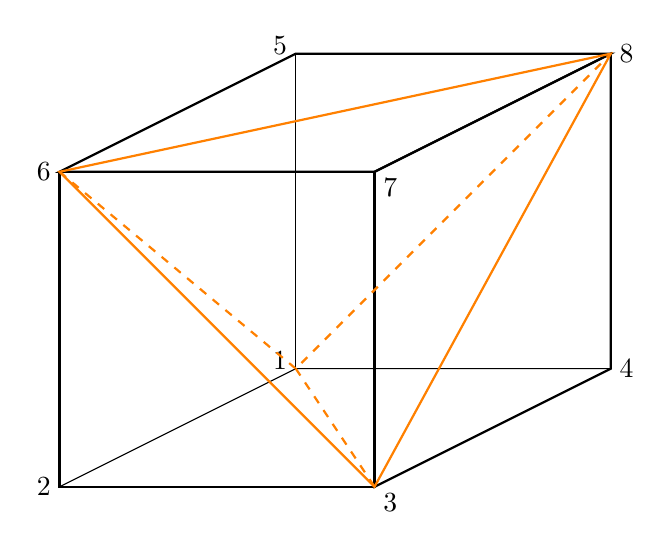
\begin{tikzpicture}
%\draw[step=0.5cm,gray,very thin] (0,0) grid (8,7); 
\draw[thick] (1,1)--(5,1)--(5,5)--(1,5)--cycle;
\draw[thick] (5,1)--(8,2.5)--(8,6.5)--(5,5)--cycle;
\draw[thick] (1,5)--(5,5)--(8,6.5)--(4,6.5)--cycle;
\draw[] (1,1)--(4,2.5)--(8,2.5);
\draw[] (4,2.5)--(4,6.5);
\node[] at (3.8,2.6) {$1$};
\node[] at (0.8,1) {$2$};
\node[] at (5.2,0.8) {$3$};
\node[] at (8.2,2.5) {$4$};
\node[] at (3.8,6.6) {$5$};
\node[] at (0.8,5) {$6$};
\node[] at (5.2,4.8) {$7$};
\node[] at (8.2,6.5) {$8$};
\draw[-,thick,orange] (1,5)--(5,1)--(8,6.5)--cycle;
\draw[thick,orange,dashed] (1,5)--(4,2.5)--(8,6.5);
\draw[thick,orange,dashed] (4,2.5)--(5,1);
\end{tikzpicture}
\end{center}

\begin{center}
\begin{tabular}{lcccc}
\hline
tetrahedron & node 1& node 2& node 3& node 4  \\
\hline
\hline
1&2&3&6&1 \\
2&4&1&8&3 \\
3&5&1&6&8 \\
4&7&8&6&3 \\
5&3&6&1&8 \\
\hline
\end{tabular}
\end{center}



 %%%%%%%%%%%%%%%%%%%%%%%%%%%%%%%%%%%%%%%%%%%%%%%%%%%%%%%%%%%%%%%%%%%% 

\chapter{Y12M solver for $Q_1\times P_0$+penalty Fortran codes \label{f101}} %%%%%%%%%%%%%%%%%%%%%%%%%%%%%%%% 101
\lstinputlisting[language=bash,basicstyle=\small]{python_codes/fieldstone_101/keywords.ascii}

\begin{center}
Code at \url{https://github.com/cedrict/fieldstone/tree/master/python_codes/fieldstone_101}
\end{center}

\par\noindent\rule{\textwidth}{0.4pt}

%%%%%%%%%%%%%%%%%%%%%%%%%%%%%%%%%%%%%%%%%%%%%%%%%%%%%%%%%%%%%%%%%%%%%%%%%%%%%%%%%%%%%%%%%%%%%%%%%%%%

\begin{center}
\includegraphics[width=1cm]{images/fortran/fortran} 
\end{center}

This stone explores the possibilities offered by the Y12M direct solver\footnote{
\url{http://www.netlib.org/y12m/doc}}. It is identical 
to \stone~01. Despite its age (it was published in 1981), 
this solver remains interesting because it is rather compact, has a simple interface, fits in 
a single file and relies on a sparse storage for the FE matrix.

The documentation \cite{zlws81} states:
"The Y12M is a package of Fortran subroutines for the solution of large and sparse systems of
linear algebraic equations developed at the Regional Computing Centre at the University of
Copenhagen (RECKU). Gaussian elimination and pivotal interchanges are used to factorize
the matrix of the system into two triangular matrices L and U. An attempt to control the
magnitude of the non-zero elements in order to avoid overflows or underflows and to detect
singularities is carried out during the process of factorization, lterative refinement of the first
solution may be performed. It is verified (by a large set of numerical examples) that iterative
refinement combined with a large drop-tolerance and a large stability factor is often very
successful when the matrix of the system is sparse, Not only is the accuracy improved but
the factorization time is also considerably reduced so that the total computing time for the
solution of the system with iterative refinement is less than that without iterative refinement
(in some examples the total computing time was reduced by more than three times). The
storage needed can often be reduced also."

The Y12M solver comes in two versions Y12MAE (single precision) and Y12MAF (double precision).
We obviously use the latter in the code. 
This solver requires the matrix to be stored in COO coordinates, not CSR nor CSC.
The non-zero entries are then stored in two integer arrays SNR and RNR of length Nfem:
\begin{itemize}
\item SNR - INTEGER array. On entry SNR(j) must contain the
column number of the non-zero element stored in A(j).
The content of array SNR is modified by
subroutine Y12MA. 
\item RNR - INTEGER array. On entry RNR(i) must contain the row
number of the non-zero element stored in A(i).
The content of array RNR is modified by subroutine Y12MA.
\end{itemize}
Note that since I had the code for building the CSR arrays I build these and use them to fill SNR and RNR:
\begin{lstlisting}[language=Fortran]
nz=0
snr(1)=1
rnr(1)=1
ia(1)=1
do j1=1,nny
do i1=1,nnx
   ip=(j1-1)*nnx+i1 ! node number
   do k=1,ndof
      ii=2*(ip-1) + k ! address in the matrix
      nsees=0
      do j2=-1,1 ! exploring neighbouring nodes
      do i2=-1,1
         i=i1+i2
         j=j1+j2
         if (i>=1 .and. i<= nnx .and. j>=1 .and. j<=nny) then ! if node exists
            jp=(j-1)*nnx+i  ! node number of neighbour 
            do l=1,ndof
               jj=2*(jp-1)+l  ! address in the matrix
               nz=nz+1
               snr(nz)=ii
               rnr(nz)=jj
               ja(nz)=jj
               nsees=nsees+1
            end do
         end if
      end do
      end do
      ia(ii+1)=ia(ii)+nsees
   end do ! loop over ndofs
end do
end do
\end{lstlisting}
This algorithm only works when the mesh is structured and linear elements are used. Also, 
despite the matrix being symmetric it must be stored in its entirety here. 

The code can be compiled by means of the {\filenamefont compile} script (you may need to 
modify it to make it compatible with your machine) and the code is executed by running
the generated {\filenamefont simplefem} executable.  

There is a built-in loop in the code which varies resolutions from $8\times 8$ to $256\times 256$.
We can then look at the solve time as a function of velocity degrees of freedom: 

\begin{center}
\includegraphics[width=10cm]{python_codes/fieldstone_101/results/timings.pdf}
\end{center}

It carries out a solve on a $256\times 256$ mesh in about 130s. This is of course rather slow when compared to 
MUMPS performance, but it allows for plenty of testing.
The code also computes the root mean square velocity and we can see that it becomes more and more accurate with 
an increase in resolution (i.e. a decrease in element size $h$), which is also confirmed by looking at the 
velocity error convergence, found to be quadratic as expected (see \stone 1):

\begin{center}
\includegraphics[width=7cm]{python_codes/fieldstone_101/results/vrms.pdf}
\includegraphics[width=7cm]{python_codes/fieldstone_101/results/errv.pdf}
\end{center}


 %%%%%%%%%%%%%%%%%%%%%%%%%%%%%%%%%%%%%%%%%%%%%%%%%%%%%%%%%%%%%%%%%%%%

\chapter{conformal mesh refinement in 2D \label{f102}} %%%%%%%%%%%%%%%%%%%%%%%%%%%%%%%%%%%%%%%%%%%%%%%%%%%%%% 102
\lstinputlisting[language=bash,basicstyle=\small]{python_codes/fieldstone_102/keywords.ascii}

\begin{center}
Code at \url{https://github.com/cedrict/fieldstone/tree/master/python_codes/fieldstone_102}
\end{center}

\par\noindent\rule{\textwidth}{0.4pt}

%%%%%%%%%%%%%%%%%%%%%%%%%%%%%%%%%%%%%%%%%%%%%%%%%%%%%%%%%%%%%%%%%%%%%%%%%%%%%%%%%%%%%%%%%%%%%%%%%%%%


\begin{center}
\includegraphics[width=1cm]{images/fortran/fortran} 
\end{center}

The topic of Conformal Mesh Refinement is introduced in Section~\ref{ss:cmr}.
This stone is a 'simple' approach to the implementation of Conformal Refinement. The code was written 
a few years prior to my working on fieldstone, so it is in Fortran. It is a 
simple Finite Element code which relies on $Q_1\times P_0$ elements. It solves the 
manufactured solution problem of Section~\ref{mms1}.

Let us start with a very simple test: the mesh counts $9\times 7=63$ elements.
The greyed elements are those to be refined. We then first flag 
the nodes which compose them and these are shown in teal color.
Based on this information we can then consider each element in the mesh and assign it a type, 
based on whether or not one or more nodes are flagged: 

\begin{center}
\input{tikz/tikz_cr_1}
\end{center}

The type is stored in the elemental array {\tt crtype} while the nodes belonging to elements 
to be refined are stored in {\tt crnode}.
There are 15 types of elements (the element type is tied to how many and which vertices are flagged nodes):

\begin{center}
\input{tikz/tikz_cr_2}
\end{center}

Note that the refinement above is based on a 3x3 refinement of elements. One could also carry out a 5x5-type
refinement which would then rely on the following elements (and their rotated versions)\footnote{I have never
seen a concrete example of these...}:
\begin{center}
\input{tikz/tikz_cr_3}
\end{center}

After running the code, various vtu files are to be found in the OUT folder.
{\filenamefont solution.vtu} contains the refined mesh with the calculated 
solution. 

\newpage
%................................................................
\paragraph{Case test=0}

The domain size is 9x7 and nelx=9, nely=7, so that all elements are square. 
The code solves the FE system but it is pointless as this test is about demonstrating 
the resulting mesh from the flagged elements at the beginning of this stone. 

\begin{center}
a)\includegraphics[width=7cm]{python_codes/fieldstone_102/results/test0/mesh1}
b)\includegraphics[width=7cm]{python_codes/fieldstone_102/results/test0/mesh2}\\
c)\includegraphics[width=7cm]{python_codes/fieldstone_102/results/test0/mesh3}
d)\includegraphics[width=7cm]{python_codes/fieldstone_102/results/test0/mesh4}\\
{\captionfont a) original mesh. b) flagged nodes. c) element types. d) refined mesh.}
\end{center}

%................................................................
\paragraph{Case test=1,2,3}

\begin{center}
\includegraphics[width=5.6cm]{python_codes/fieldstone_102/results/test1/vel}
\includegraphics[width=5.6cm]{python_codes/fieldstone_102/results/test2/vel}
\includegraphics[width=5.6cm]{python_codes/fieldstone_102/results/test3/vel}\\
\includegraphics[width=5.6cm]{python_codes/fieldstone_102/results/test1/press}
\includegraphics[width=5.6cm]{python_codes/fieldstone_102/results/test2/press}
\includegraphics[width=5.6cm]{python_codes/fieldstone_102/results/test3/press}\\
{\captionfont Initial resolution 10x10. 
Left: The left half of elements are flagged for refinement.
Middle: The elements above the diagonal are flagged for refinement.
Right: Every 7 elements is flagged for refinement.}
\end{center}

















 %%%%%%%%%%%%%%%%%%%%%%%%%%%%%%%%%%%%%%%%%%%%%%%%%%%%%%%%%%%%%%%%%%%%

\chapter{conformal mesh refinement in 3D \label{f103}} %%%%%%%%%%%%%%%%%%%%%%%%%%%%%%%%%%%%%%%%%%%%%%%%%%%%%% 103
\includegraphics[height=1.25cm]{images/pictograms/tools}
\includegraphics[height=1.25cm]{images/pictograms/3d}

%%%%%%%%%%%%%%%%%%%%%%%%%%%%%%%%%%%%%%%%%%%%%%%%%%%%%%%%%%%%%%%%%%%%%%%%%%%%%%%%%%%%%%%%%%%%%%%%%%%

\lstinputlisting[language=bash,basicstyle=\small]{python_codes/fieldstone_103/keywords.ascii}

\begin{center}
\fbox{\textbf{\huge \color{orange} F}}
Code at \url{https://github.com/cedrict/fieldstone/tree/master/python_codes/fieldstone_103}
\end{center}

\par\noindent\rule{\textwidth}{0.4pt}

%%%%%%%%%%%%%%%%%%%%%%%%%%%%%%%%%%%%%%%%%%%%%%%%%%%%%%%%%%%%%%%%%%%%%%%%%%%%%%%%%%%%%%%%%%%%%%%%%%%%

The topic of Conformal Mesh Refinement is introduced in Section~\ref{MMM-ss:cmr}.
This code is in Fortran for the same reason \stone~102 is. 
However, it is not nearly as complete as \stone~102: It can only refine 
above a certain height, as the different types of subdivisions are not implemented.
Furthermore, there is no FE solver in it either. It is just an example of 
simple 3D conformal refinement meshing.

The {\filenamefont prog.f90} code showcases the decomposition of one element and generates
the {\filenamefont refined.vtu} file:
\begin{center}
\includegraphics[width=4.5cm]{python_codes/fieldstone_103/visu1}
\includegraphics[width=4.5cm]{python_codes/fieldstone_103/visu2}
\includegraphics[width=4.5cm]{python_codes/fieldstone_103/visu3}
\end{center}
The internal numbering goes as follows:
\begin{center}
\includegraphics[width=7cm]{python_codes/fieldstone_103/images/numbering}\\
{\captionfont Taken from ? Numbers added by me. There are additional handwritten notes
in the images folder.}
\end{center}

In order to finish the {\filenamefont stone.f90} code, one would need to 
implement all four (+rotations) of these subdivisions:
\begin{center}
\includegraphics[width=8cm]{python_codes/fieldstone_103/images/scde}\\
{\captionfont Taken from ?}
\end{center}

Note that there is another way to subdivide an element:
\begin{center}
\includegraphics[width=5cm]{python_codes/fieldstone_103/images/habo04}\\
{\captionfont Taken from \cite{habo04}.}
\end{center}

Finally, we can run the code on a $20\times16\times12$ original mesh:
\begin{center}
\includegraphics[width=7cm]{python_codes/fieldstone_103/before}
\includegraphics[width=7cm]{python_codes/fieldstone_103/after}
\end{center}

 %%%%%%%%%%%%%%%%%%%%%%%%%%%%%%%%%%%%%%%%%%%%%%%%%%%%%%%%%%%%%%%%%%%%

\chapter{grad-div stabilisation ($Q_2\times Q_1$, $Q_2 \times P_{-1}$) \label{f104}} %%%%%%%%%%%%%%%%%%%%%%%% 104
\includegraphics[height=1.25cm]{images/pictograms/benchmark}
\includegraphics[height=1.25cm]{images/pictograms/FEM}

%%%%%%%%%%%%%%%%%%%%%%%%%%%%%%%%%%%%%%%%%%%%%%%%%%%%%%%%%%%%%%%%%%%%%%%%%%%%%%%%%%%%%%%%%%%%%%%%%%%

%\lstinputlisting[language=bash,basicstyle=\small]{python_codes/fieldstone_103/keywords.ascii}

\begin{center}
Code at \url{https://github.com/cedrict/fieldstone/tree/master/python_codes/fieldstone_104}
\end{center}

\par\noindent\rule{\textwidth}{0.4pt}

%%%%%%%%%%%%%%%%%%%%%%%%%%%%%%%%%%%%%%%%%%%%%%%%%%%%%%%%%%%%%%%%%%%%%%%%%%%%%%%%%%%%%%%%%%%%%%%%%%%


Note to self: normalisation does not work for Q2Q1.

All the following benchmarks are isoviscous with $\eta=1$ and are valid in the unit square domain. 
As such the scaling coefficient between blocks $\K$ and $\G$ of the Stokes matrix (see Section~\ref{X_Y_Z}) 
is 1 and won't play any role in the results. 

REDO all with aspect

According to Jenkins \etal (2014) \cite{jejl14}, Grad-div stabilization results from adding
$\vec{0} = - \gamma \vec\nabla (\vec\nabla\cdot \vec\upnu)$ to the continuous Stokes
equations, i.e.:
\[
-\nabla p  + \nabla \cdot ( 2 \eta \dot{\bm \varepsilon}) + \rho \vec{g} 
= - \gamma \vec\nabla (\vec\nabla\cdot \vec\upnu)
\]
We immediately notice that the aditional term is in fact identical to the penalty term and 
its weak form and discretisation is worked out in Section~\ref{X_X_X}, so that 
the matrix $\K$ then becomes:
\[
\K = \int {\bm B}^T \cdot [ \gamma {\bm K} + \eta {\bm C} ] \cdot {\bm B} \; dV
\]
with 
\[
{\bm C}=
\left(
\begin{array}{ccc}
2 & 0 & 0 \\
0 & 2 & 0 \\
0 & 0 & 1 
\end{array}
\right)
\qquad
{\bm K}=
\left(
\begin{array}{ccc}
1 & 1 & 0 \\
1 & 1 & 0 \\
0 & 0 & 0 
\end{array}
\right)
\]
The implementation is then trivial. Surprisingly in the papers on the grad-div stabilisation 
the penalty method is never mentioned (?) although John \etal state that 
"[...] it shall be emphasized that large
contributions of the grad-div stabilization result in linear systems of equations with
large condition numbers", which is a well know problem of the penalty method.

In this case $\gamma>0$ but another parallel can be drawn when $\gamma = -\frac{2}{3}\eta$. In that case
\[
 \nabla \cdot ( 2 \eta \dot{\bm \varepsilon}) + \gamma \vec\nabla (\vec\nabla\cdot \vec\upnu)
=
 \nabla \cdot ( 2 \eta \dot{\bm \varepsilon}) -\frac{2\eta}{3} \vec\nabla (\vec\nabla\cdot \vec\upnu)
=
 \nabla \cdot 2 \eta ( \dot{\bm \varepsilon} -\frac{1}{3} (\vec\nabla\cdot \vec\upnu) {\bm 1} )
= 
 \nabla \cdot 2 \eta \dot{\bm \varepsilon}^d 
\]
Obviously $\gamma$ should not be `too negative', otherwise terms on the diagonal 
of $\gamma {\bm K} + \eta {\bm C} $
will be negative and this will cause problems. 

In what follows I have implemented what I think the grad-div method is, with 
rather limited/puzzling (?) results.
Rather importantly John \etal conclude that ``the
grad-div stabilization might improve the pressure-robustness in certain situations but
it is not a remedy''. 

\Literature: \cite{ollh09}

%---------------------------------------------------------------------
\subsubsection*{Experiment=1: Donea \& Huerta manufactured solution}

I carry out this benchmark to make sure that the code behaves as expected and that the
error rates are what we expect: 3rd order for velocity, second order for pressure 
for both $Q_2\times Q_1$ and $Q_2\times P_{-1}$ elements (see for instance 
Thieulot \& Bangerth \cite{thba22}).

\begin{center}
\includegraphics[width=8cm]{python_codes/fieldstone_104/results/exp1/errors.pdf}
\end{center}


%---------------------------------------------------------------------
\subsubsection*{Experiment=2: example 1.1 in John \etal (2017)}
Following John \etal (2017) \cite{jolm17} we 
postulate the following velocity and pressure fields:
\begin{eqnarray}
\vec{\upnu}(x,y) &=& \vec{0} \nn\\
p(x,y) &=& \Ranb ( y^3-y^2/2+y-7/12 ) \nn
\end{eqnarray}
with $\eta=1$ and the buoyancy force vector is
\[
\vec{b}=
\left(
\begin{array}{c}
0 \\ \Ranb(1-y+3y^2)
\end{array}
\right)
\]

\begin{center}
\includegraphics[height=4cm]{python_codes/fieldstone_104/results/exp2/errors.pdf}
\includegraphics[height=4cm]{python_codes/fieldstone_104/results/exp2/jolm17a}\\
{\captionfont Left: this stone; Right: taken from \cite{jolm17}}
\end{center}

We find that the velocity error magnitude for the $Q_2\times Q_1$ element
scales with the Rayleigh number, and 
more surprisingly (?) that its convergence is quartic.
However, the velocity error magnitude for the $Q_2\times P_{-1}$ 
remains very low independently of the Rayleigh number

\begin{center}
\includegraphics[height=6cm]{python_codes/fieldstone_104/results/exp2/gamma/errors.pdf}
\end{center}

%---------------------------------------------------------------------
\subsubsection*{Experiment=3,4,5: }

These three manufactured solutions come from Jenkins \etal (2014) \cite{jejl14}.
The velocity is the same in all cases, $\vec{\upnu}=(\cos 2\pi y , \sin 2\pi x)$
while the three pressure fields are
\begin{eqnarray}
p_1(x,y) &=& \sin (2\pi y)  \nn\\
p_2(x,y) &=& \sin (8 \pi y)   \nn\\
p_3(x,y) &=& 10^4 \sin (2\pi y) \nn
\end{eqnarray}
We need to compute the vector $\vec{b}$ from these. 
The strain rate tensor is then 
\[
\dot{\bm \varepsilon}(\vec{\upnu}) = 
\left(
\begin{array}{cc}
0 &  - \pi \sin 2\pi y + \pi \cos 2 \pi x  \\
 - \pi \sin 2\pi y + \pi \cos 2 \pi x   & 0
\end{array}
\right)
\]
and then the full stress tensor:
\[
{\bm \sigma} = 
- p {\bm 1}+ 2 \eta \dot{\bm \varepsilon}
= \left(
\begin{array}{cc}
-p &  -2 \pi \eta (\sin 2\pi y -  \cos 2 \pi x)  \\
-2 \pi \eta (\sin 2\pi y -  \cos 2 \pi x)   & -p
\end{array}
\right)
\]
Finally
\[
-\vec{b} = 
\vec\nabla \cdot {\bm \sigma} = 
\left(
\begin{array}{c}
-\partial_x p - 4 \pi^2 \eta \cos 2\pi y  \\ 
-\partial_y p - 4 \pi^2 \eta \sin 2\pi x 
\end{array}
\right)
\]
We see that we have $\partial_x p_{1,2,3} =0$ so 
\[
\vec{b}
=
\left(
\begin{array}{c}
 4 \pi^2 \eta \cos 2\pi y  \\ 
\partial_y p + 4 \pi^2 \eta \sin 2\pi x 
\end{array}
\right)
\]

\begin{center}
\includegraphics[width=5cm]{python_codes/fieldstone_104/results/exp3/errors.pdf}
\includegraphics[width=5cm]{python_codes/fieldstone_104/results/exp4/errors.pdf}
\includegraphics[width=5cm]{python_codes/fieldstone_104/results/exp5/errors.pdf}
\end{center}

We see that the Q2Q1 velocity error is much larger than the Q2P1 error in benchmark 3 
but that it converges again in a quartic manner.
Pressure errors are however identical.

%------------------------------------------------------------------------------------------
\subsubsection*{Experiment=6: manufactured solution in John \etal (2017) \cite{jolm17}}

See Section~\ref{MMM-ss:mmsjolm17} for details.

\begin{center}
\includegraphics[width=5cm]{python_codes/fieldstone_104/results/exp6/vel}
\includegraphics[width=5cm]{python_codes/fieldstone_104/results/exp6/press}
\includegraphics[width=5cm]{python_codes/fieldstone_104/results/exp6/errors.pdf}
\end{center}


\begin{center}
\includegraphics[height=6cm]{python_codes/fieldstone_104/results/exp6/gamma/errors.pdf}\\
{\captionfont errors as a function of $\gamma$.}
\end{center}

\vspace{2cm}

\Literature: 
\textcite{hera13}



 %%%%%%%%%%%%%%%%%%%%%%%%%%%%%%%%%%%%%%%%%%%%%%%%%%%%%%%%%%%%%%%%%%%%

\chapter{solving the flexure equation with FDM  \label{f105}} %%%%%%%%%%%%%%%%%%%%%%%%%%%%%%%%%%%%% 105
\includegraphics[height=1.5cm]{images/pictograms/elasticity}
\includegraphics[height=1.5cm]{images/pictograms/benchmark}

\lstinputlisting[language=bash,basicstyle=\small]{python_codes/fieldstone_105/keywords.ascii}

\begin{center}
Code at \url{https://github.com/cedrict/fieldstone/tree/master/python_codes/fieldstone_105}
\end{center}

\par\noindent\rule{\textwidth}{0.4pt}

{\sl This stone was developed in collaboration with Zolt{\'a}n Erd{\H{o}}s}. 
\index{contributors}{Z. Erd{\H{o}}s}

\par\noindent\rule{\textwidth}{0.4pt}

%%%%%%%%%%%%%%%%%%%%%%%%%%%%%%%%%%%%%%%%%%%%%%%%%%%%%%%%%%%%%%%%%%%%%%%%%%%%%%%%%%%%%%%%%%%%%%%%%%%%

Under many simplifying approximations (See Section~3.9 of Turcotte \& Schubert book \cite{tusc}), 
the simplest time-independent flexure equation is
\[
D \frac{d^4w(x)}{dx^4} + P \frac{d^2w(x)}{dx^2} + (\rho_m-\rho_c)g w(x) = q(x)
\]
where $w(x)$ is the plate deflection (\si{m}), 
\[
D=\frac{E t^3}{12(1-\nu^2)}
\]
is the flexural rigidity, with $t$ the thickness of the plate (\si{m}), 
$E$ is Young's modulus, $\nu$ is the Poisson ratio, 
$P$ is a horizontal force per unit length (\si{\kg\per\square\metre\square\sec}),  
$q$ is the load (\si{\pascal}), 
$\rho_m$ is the mantle density and $\rho_c$ is the density of the crust (\si{\kg\per\cubic\metre}).
This is a 4th-order ODE. In order to solve it, we will need 4 boundary conditions.

Redo Fig. 3.24 of T\&S. 

We wish to solve this equation on the domain $[0,L_x]$ with the Finite Difference method. 
Indeed the presence of a 4th-order derivative poses quite a few problems for the Finite Element 
method and in this case the FDM is more straighforward to implement (see also 
discussion in Section~2.3 of Buiter \cite{buiter_thesis}). 
The domain is discretised with $n_p$ nodes equally spaced by $h=L_x/(n_p-1)$.

We will need the 2nd- and 4th-order 
derivatives\footnote{\url{https://en.wikipedia.org/wiki/Finite_difference_coefficient}}:
\begin{eqnarray}
\frac{d^2w}{dx^2} &=& \frac{w_{n-1}-2w_n+w_{n+1}}{h^2} 
+{\cal O}(h^3) \\
\frac{d^4w}{dx^4} &=& \frac{w_{n-2}-4w_{n-1}+6w_n-4w_{n+1}+w_{n+2}}{h^4}
+{\cal O}(h^5)
\end{eqnarray}
Both are second-order accurate. We then obtain 
\[
D\frac{w_{n-2}-4w_{n-1}+6w_n-4w_{n+1}+w_{n+2}}{h^4}
+P\frac{w_{n-1}-2w_n+w_{n+1}}{h^2} 
+(\rho_m-\rho_c)g w_n = q_n
\]
or, 
\[
\boxed{
\frac{D}{h^4} w_{n-2}
+\left(-\frac{4D}{h^4}+\frac{P}{h^2}\right)w_{n-1}
+\left(\frac{6D}{h^4}-\frac{2P}{h^2} +(\rho_m-\rho_c)g \right)w_n
+\left(-\frac{4D}{h^4}+\frac{P}{h^2}\right)w_{n+1}
+\frac{D}{h^4} w_{n+2} = q_n
}
\]
One could also multiply this equation by $h^4$ and obtain:
\[
D w_{n-2}
+\left(-4D+Ph^2\right)w_{n-1}
+\left(6D-2Ph^2 +(\rho_m-\rho_c)g h^4 \right)w_n
+\left(-4D+Ph^2\right)w_{n+1}
+D w_{n+2} = q_n h^4
\]
We will formulate this equation for every node $i\in[2,n_p-3]$
in a systematic manner and we will therefore obtain a linear system of equations of the form 
\[
{\bm A} \cdot \vec{w} = \vec{b}
\]
where ${\bm A}$ is an $n_p\times n_p$ matrix (sparse since pentadiagonal) 
and $\vec{b}$ the right-hand side vector. 
The vector $\vec{w}$ contains the $n_p$ deflection unknowns at the nodes of the mesh.

\begin{center}
\includegraphics[width=4cm]{python_codes/fieldstone_105/images/matrix}
\end{center}

The four missing lines are addressed when we consider the boundary conditions:
We assume the plate to be very long, and that the load(s) will be 
mostly concentrated around $L_x/2$ . We therefore 
prescribe $w=0$ and $dw/dx=0$ at $x=0$ and $x=L_x$ (i.e. the deflection and 
the slope at the edges of the beam both tend to zero).

The first condition is trivial to impose: set 1 on the diagonal of the 
matrix for $i=0$ and $i=n_p-1$ and the corresponding entries of the rhs to zero. 
The second will have us use the backward derivative on the left for node $i=1$ and 
the forward derivative on the right for node $n_p-2$:
\begin{eqnarray}
\frac{dw}{dx} (x=0)   &\simeq& \frac{-w_0+w_1}{h} \nonumber\\
\frac{dw}{dx} (x=L_x) &\simeq& \frac{-w_{n_p-2}+w_{n_p-1}}{h}
\end{eqnarray}
The two equations will replace the second and before last 
lines in the matrix.

The flexure equation which allows for $D$ to be a function of space is 
\[
\frac{d^2}{dx^2} \left( D(x) \frac{d^2w(x)}{dx^2} \right) + P \frac{d^2w(x)}{dx^2} 
+ (\rho_m-\rho_c)g w(x) = q(x)
\]
Instead of using the expression for a 4th-order derivative we then use the expression 
for a 2nd-order derivative twice. 
Let us temporarily coin $\phi=D(x) \frac{d^2w}{dx^2}$.
Then
\begin{eqnarray}
&&\frac{d^2}{dx^2} \left( D(x) \frac{d^2w(x)}{dx^2} \right)\\
&=& \frac{d^2 \phi}{dx^2} \\
&\simeq& \frac{\phi_{n-1}-2\phi_n+\phi_{n+1}}{h^2} \nonumber\\
&\simeq& \frac{1}{h^2}
\left(
D_{n-1} \frac{w_{n-2}-2w_{n-1}+w_{n}}{h^2}
-2 D_n \frac{w_{n-1}-2w_n+w_{n+1}}{h^2}
+ D_{n+1} \frac{w_{n}-2w_{n+1}+w_{n+2}}{h^2}
\right) \nonumber\\
&=&
\frac{D_{n-1}}{h^4} w_{n-2}
-2\frac{D_{n-1}+D_n}{h^4} w_{n-1}
+\frac{D_{n-1}+4D_n+D_{n+1}  }{h^4} w_n
-2\frac{D_{n}+D_{n+1}}{h^4} w_{n+1}
+\frac{D_{n+1}}{h^4} w_{n+2} \nonumber
\end{eqnarray}
Obviously if $D_{n-1}=D_n=D_{n+1}$ we recover the 
expression above derived with a constant flexural 
rigidity $D$.
The full flexural equation with the variable $D(x)$ then reads as
\begin{eqnarray}
\frac{D_{n-1}}{h^4} w_{n-2}
+\left(-2\frac{D_{n-1}+D_{n}}{h^4}+\frac{P}{h^2}\right)w_{n-1}
+\left(\frac{D_{n-1}+4D_{n}+D_{n+1}}{h^4}-\frac{2P}{h^2} +(\rho_m-\rho_c)g \right)w_n \nonumber\\
+\left(-2\frac{D_{n}+D_{n+1}}{h^4}+\frac{P}{h^2}\right)w_{n+1}
+\frac{D_{n+1}}{h^4} w_{n+2} = q_n
\end{eqnarray}

In what follows the material parameters are those of Fig.~2.2 in Buiter \cite{buiter_thesis}:
$t=10\si{\km}$, $\nu=0.25$, $W=10^{11}\si{\pascal}$, $\rho_m=3250\si{\kg\per\cubic\metre}$, 
$\rho_c=2800\si{\kg\per\cubic\metre}$.

\Literature: Section 11 in Simpson's book \cite{simp17}

%-------------------------------------------------
\subsubsection*{Benchmark 1: line load}

Following Buiter (2000) \cite{buiter_thesis} we consider the case of a lineload.
The lineload $F$ is applied in the middle of the domain and the solution 
is therefore symmetric around $x=L_x/2$.
The analytical solution is given by\footnote{I believe the absolute values
were missing in the thesis.} 
\[
w_{analytical} = \frac{F \alpha^3}{8 D} \exp -\frac{|x|}{\alpha}
\left(
\cos \frac{|x|}{\alpha} + \sin \frac{|x|}{\alpha} 
\right)
\]
with the so-called flexural parameter \index{general}{Flexural Parameter} 
\[
\alpha=\left(\frac{4D}{(\rho_m-\rho_c)g}\right)^{1/4}
\]
which measures the wavelength of the flexure.

\begin{center}
\includegraphics[width=5cm]{python_codes/fieldstone_105/images/buiter}
\includegraphics[width=8cm]{python_codes/fieldstone_105/results/bench1/w.pdf}\\
{\captionfont Left: Taken from \cite{buiter_thesis}}
\end{center}


%-------------------------------------------------
\subsubsection*{Benchmark 2: periodic loading}

For this benchmark we only prescribe $w=0$ at both extremities.
For the second and before last lines of the matrix we resort to 
using forward and backward expressions for the 4th-order 
derivative for simplicity.
The load is given by:
\[
q(x)=\rho_c g h_0 \sin 2\pi \frac{x}{\lambda}
\]
The solution is $w(x)=w_0 \sin 2\pi x/\lambda$, with 
\[
w_0=\frac{h_0}{\frac{\rho_m}{\rho_c}-1+\frac{D}{\rho_c g} (2\pi/\lambda)^4}
\]

\begin{center}
\includegraphics[width=8cm]{python_codes/fieldstone_105/results/bench2/w.pdf}\\
{\captionfont Obtained with $\lambda=0.5Lx$}
\end{center}

%-------------------------------------------------
\subsubsection*{Experiment 3: island}

The load is given by $q(x)=-\rho_c g h_0 \left(1+\cos 2\pi \frac{|x-L_x/2|}{\lambda}\right) $
for $|x-L_x/2|<\lambda/2$ 

\begin{center}
\includegraphics[width=8cm]{python_codes/fieldstone_105/results/exp3/load}
\includegraphics[width=8cm]{python_codes/fieldstone_105/results/exp3/w.pdf}\\
{\captionfont Obtained with $\lambda=0.1$. Left: load; Right: deflection.}
\end{center}

-------------------

\Literature: \fullcite{debr77}\\
\fullcite{beau78}

 %%%%%%%%%%%%%%%%%%%%%%%%%%%%%%%%%%%%%%%%%%%%%%%%%%%%%%%%%%

\chapter{plumes in axisymmetric chunk ($Q_2\times Q_1$)  \label{f106}} %%%%%%%%%%%%%%%%%%%%%%%%%%%% 106
\lstinputlisting[language=bash,basicstyle=\small]{python_codes/fieldstone_106/keywords.ascii}

\begin{center}
Code at \url{https://github.com/cedrict/fieldstone/tree/master/python_codes/fieldstone_106}
\end{center}

\par\noindent\rule{\textwidth}{0.4pt}

\Literature Kiefer \& Hager \cite{kiha92}, King \cite{king97}, Redmond \& King \cite{reki04},
Kiefer (2003) \cite{kief03}, Li \& Kiefer (2007) \cite{liki07}

\par\noindent\rule{\textwidth}{0.4pt}
%%%%%%%%%%%%%%%%%%%%%%%%%%%%%%%%%%%%%%%%%%%%%%%%%%%%%%%%%%%%%%%%%%%%%%%%%%%%%%%%%%%%%%%%%%%%%%%%%%%%

This stone is inspired by Kellogg \& King (1997) \cite{keki97}. 

\begin{center}
\includegraphics[width=6cm]{python_codes/fieldstone_106/images/keki97a}\\
{\captionfont Taken from \cite{keki97}.}
\end{center}

I set out to reproduce the results of the original publication. 
The necessary information is spread out throughout the first pages.
In Section~3 it is stated that the angular opening is $\pi/4$ and $r_i/r_o=0.55$.
However, it is not clear what $r_i$ or $r_o$ are, although Section~3
mentions $r$ values of 1.7 which is somewhat in the 'middle' of the cone. 
Because the equations in the paper are in dimensionless form, and 
because it is common to choose the depth of the mantle as reference length, 
then we probably have $r_o-r_i=1$. In this case we find $r_i=1.22\dots$ and 
$r_o=2.22\dots$ ({\color{orange} 1st guess}: confirmed by author S.K., June 2021. 
Also consistent with King \cite{king97}).

Free-slip boundary conditions are imposed on all boundaries.
A patch on the inner boundary of the shell is heated by
maintaining it at a constant dimensionless temperature of $T_{patch}=1$; 
elsewhere the base of the shell is insulating ($\partial T/\partial r = 0$).
At the top of the shell, a constant dimensionless temperature of $T_{top}=0$ was maintained.
Unfortunately it is not specified how wide the patch is, so I choose 
$\pi/8$ which seems probable when looking at 
Figure~3 of the paper ({\color{orange} 2nd guess}: confirmed by S.K., June 2021).
The sides of the cone are insulating ($\partial T/\partial \theta =0$).
Because of how FE works the insulating boundary conditions are automatically enforced 
when Dirichlet boundary conditions are absent. 

The viscous rheology is temperature-dependent:
\[
\eta(T) =\eta_0 \exp\left[ E \left( \frac{1}{T+T_0} -\frac{1}{1+T_0}  \right)   \right]
\]
with $E= \{0,0.25328,3\}$. $T_0$ is defined as ``the surface temperature divided by the temperature
drop across the shell'' but its value is not specified. On Earth the surface temperature 
is $\sim300\si{\kelvin}$
while the temperature drop across the mantle is $\sim3000\si{\kelvin}$ 
so I take $T_0=0.1$ ({\color{orange} 3rd guess}: S.K. says that $\Delta T$ can be recovered from 
the Rayleigh number and using standard Earth values for all other parameters, but given the uncertainty about 
the Rayleigh number itself, this parameter is lost forever).
The value for $\eta_0$ is also not specified but if this value is used as reference viscosity value 
during the adimensionalisation process then $\eta_0=1$ ({\color{orange} 4th guess}).i
As indicated in the paper, the viscosity is ``clipped'' to $1000\eta_0$.
The initial temperature in the domain is set to $T=0.25$.

As seen in Section~\ref{ss:dimeqs2}, the dimensionless heat transport equation is void of any coefficient if 
$\kappa/h$ is used as a reference velocity (where $h$ is a reference length) so we take the 
dimensionless value of $\kappa$ to be 1 in Eq.~5 of the paper.   

Looking at Eq.~1 we find that there probably is a factor 2 missing before 
the viscosity $\mu$ ({\color{orange} 5th guess}: confirmed by S.K., June 2021).
In Section~2.2 it is stated that the SUPG method is used (see Section~\ref{ss:supg}) 
but how the stabilisation parameter
is chosen is not specified ({\color{orange} 6th guess}).

In the end the set of equations solved by the code is as follows:
\begin{eqnarray}
-\vec\nabla p + \vec\nabla \cdot(2 \eta \dot{\bm \varepsilon} ) &=& \Ranb \; T \vec{e}_r \\
\vec\nabla\cdot\vec\upnu &=& 0 \\
\frac{\partial T}{\partial t} + \vec\upnu\cdot\vec\nabla T &=& \Delta T 
\end{eqnarray}
Given the above boundary conditions, initial temperature and Rayleigh number value $\Ranb=10^7$ these
equations can be solved. 

Concerning the value of $\Ranb$, it is said to be $10^7$ but preliminary runs (in 2D) yield much 
narrower plumes for the isoviscous case than in the paper. However using $10^6$ 
instead seems to visually match the paper's results. I asked S.K. whether 
there could not be a mistake in the reported Ra in the paper and he kindly answered the following:
"A mistake is always possible. Here’s a possibility: the $\Ranb=10^7$ was what was input into the 
input file but we did not do a proper internal scaling to account for this, i.e. 
$r_o^3$ was used rather than $(r_o-r_i)^3$ with $r_o^3 = 2.22^3 \sim 10$.  
Usually in our codes what we put in as the Rayleigh number is really rho-g-alpha and all the other factors are 
input as 1 (or implicitly assumed to be 1).  
At any rate, I suspect $10^6$ could be a result of not accounting properly for the radius not being 1.0.  
I found some files one of my students used circa 2007 and the Ra was set to $10^7$ in the input file 
while the grid (different file) was $1.2 \rightarrow 2.2$.  I could see how one would forget 
when it comes to writing up the paper."

The paper mentions dimensioned quantities twice: in the caption of Fig.~3, we 
learn that 
$t=0.000561$ corresponds to $1.5\cdot 10^8\si{\year}$,
$t=0.000730$ corresponds to $2.0\cdot 10^8\si{\year}$, and
$t=0.016353$ corresponds to $4.4\cdot 10^9\si{\year}$.
This yields a reference time of about 270e9, which is close 
to  the one obtained as $t_{ref}=h^2/\kappa = (2891e3)^2/10^{-6}\sim 8.36\cdot 10^{18}s \sim 265\cdot 10^9 \si{\year}$
(see Section~\ref{ss:dimeqs2}).

This stone relies on $Q_2\times Q_1$ elements while the orginal paper relies
on the cheaper $Q_1\times P_0$ element with a penalty formulation (the 
value of the penalty parameter is also not mentioned). 

The user chooses the number of elements in the 
radial direction $nelr$ and the number of elements in the tangential direction is automatically 
computed as $nelt=1.5\cdot nelr$.
Elements on the boundaries are flagged by means of the $flag\_el\_X$ array ($X=1,2,3,4$ 
corresponding to left, right, bottom and top). 
Similar boolean arrays are setup for nodes on the boundaries: $flag\_X$. 
Free-slip boundary conditions are more difficult to impose than for Cartesian domains 
because the boundaries of the computational domain are either curved and/or not aligned
with the Cartesian axis. 
The timestep is computed by means of a CFL criterion, but it is limited to a $2\times$ 
increase from one time step to the next to insure a somewhat smooth transition at 
the beginning when the plume is rising faster and faster.
Because the lithostatic pressure does not contribute to the calculations and has effectively
been removed from the equations the pressure that is being solved for is the dynamic pressure. 
We can therefore run models with open boundary conditions on the side walls. This is 
controlled by the $use\_fs\_on\_sides$ parameter. If this parameter is true then there is a 
rotational nullspace and it is removed by setting $\vec\upnu=\vec{0}$ at $x=0$ and $y=r_i$.
This option was not explored in the original paper.

The equations are solved in their cylindrical axisymmetric form, see
Section~\ref{ss:axicyleqs}. Their FE discretisation is presented in Section~\ref{ss:cyl_axi}
and Section~\ref{ss:hte_axisym}.


\begin{remark}
LK filter and/or SUPG should be tested (at the moment the temperature us thresholded in the 
material model). Explore resolution, initial T in the mantle, try scaled-down Steinberger average 
viscosity profile, look at dynamic topography, strain-rate dependent power-law rheology, different 
Ra number, ... finish scaling up to real Earth like dimensions.
Would be nice to normalise the pressure on the top surface, not only a corner.
Also remove all bc on sides and use reduced density only? 
\end{remark}

%------------------------------------------------
\subsubsection*{Computing surface tractions}

Pressure normalised to be zero in the upper right corner so as to remove the nullspace. 
It is then projected onto the velocity nodes. This quantity is then normalised so that 
the average pressure at the surface is zero. 

Because of the axisymmetry the deviatoric stress tensor and stress tensor 
are given by
\[
{\bm \tau} 
= 
\left(
\begin{array}{ccc}
\tau_{rr} & \tau_{r\theta} & \tau_{rz} \\
\tau_{\theta r} & \tau_{\theta \theta} & \tau_{\theta z} \\
\tau_{zr} & \tau_{z\theta} & \tau_{zz} 
\end{array}
\right)
=
\left(
\begin{array}{ccc}
\tau_{rr} & 0 & \tau_{rz} \\
0  & \tau_{\theta \theta} & 0 \\
\tau_{zr} & 0 & \tau_{zz} 
\end{array}
\right)
\qquad
\text{and}
\qquad
{\bm \sigma} = -p {\bm 1} + {\bm \tau}
\]
The traction at the surface is given by 
\[
\vec{t}_n 
= {\bm \sigma}\cdot \vec{n}
=
\left(
\begin{array}{c}
\sigma_{rr} n_r + \sigma_{rz} n_z \\
0 \\
\sigma_{zr} n_r + \sigma_{zz} n_z
\end{array}
\right)
\]
and the normal component of the traction by 
\[
t_n= \vec{t}_n \cdot \vec{n} = \sigma_{rr} n_r^2 + 2 \sigma_{rz} n_r n_z + \sigma_{zz} n_z^2
\]




%%%%%%%%%%%%%%%%%%%%%%%%%%%%%%%%%%%%%%%%%%%%%%%%%%%
\subsubsection*{Scaling it back up}

What follows is an attempt at using the regular equations with Earth-like values for parameters...

As explained in Section~\ref{ss:dimeqs2} we choose four reference quantities:
\begin{itemize}
\item the reference length $L_{ref}=r_o-r_i=2891\si{\kilo\metre}$ (trivial choice)
with $r_i=3480\si{\km}$ and $r_o=6371\si{\km}$.


\item the reference temperature $T_{ref}=\Delta T = 3000\si{\kelvin}$ (trivial choice)

\item the thermal diffusion coefficient $\kappa_{ref}$. From Warren \etal \cite{wabj08}:
$\rho_0=3250\si{\kg\per\cubic\metre}$,  $k=2.25 \si{\watt\per\metre\per\kelvin}$,  $C_p=1250 \si{\joule\per\kelvin}$
so 
\[
\kappa = \frac{k}{\rho C_p} =	\frac{2.25}{3250 \cdot 1250} \simeq 5.5\cdot 10^{-7} 
\]
so we take $\kappa_{ref} = 5.5\cdot 10^{-7} \si{\square\metre\per\second}$.

\item the reference viscosity $\eta_{ref}$. The Rayleigh number is defined by
\[
\Ranb 
= \frac{\rho_0 g \alpha \Delta T (r_o-r_i)^3}{\eta_0 \kappa}
=\frac{\rho_0^2 C_p g \alpha \Delta T (r_o-r_i)^3}{\eta_0 k}
\]
with $\alpha=3\cdot 10^{-5} \si{\per\kelvin}$ and $g=9.81\si{\metre\per\square\second}$
so 
\[
\eta_{ref}=\eta_0 =\frac{\rho_0^2 C_p g \alpha \Delta T (R_{outer}-R_{inner})^3}{\Ranb \; k}
\simeq 1.25 \cdot 10^{22}\si{\pascal\second}
\]
which is a very acceptable value for the mantle viscosity, see Section~\ref{ss:viscprof}.
\end{itemize}

\noindent The dimensionless viscosity is either constant ($\eta_0'=1$) or temperature-dependent 
\[
\eta'(T')
=\eta_0' \exp\left[ \frac{E}{R \Delta T} \left( \frac{1}{T'+t_0} -\frac{1}{1+t_0}  \right)   \right]
%=\eta_0' \exp\left[ \frac{E}{R} \left( \frac{1}{T' \Delta T  +t_0 \Delta T} -\frac{1}{\Delta T +t_0 \Delta T}  \right)   \right]
\]
where ``$t_0$ is the surface temperature $T_{surf}$ divided by 
the temperature drop across the shell $\Delta T$''.
Assuming that the authors used 
\[
T'=\frac{T-T_{surf}}{T_{patch}-T_{surf}}= \frac{T-T_{surf}}{\Delta T}
\]
then (after multiplying the equation above by $\eta_{ref}$): 
\[
\eta(T)
=\eta_0 \exp\left[ \frac{E}{R} \left( \frac{1}{T-T_{surf}  + T_{surf}} 
-\frac{1}{T_{patch}-T_{surf} + T_{surf}}  \right)   \right]
=\eta_0 \exp\left[ \frac{E}{R} \left( \frac{1}{T} -\frac{1}{T_{patch}}\right) \right]
\]
so that $\eta(T_{patch})=\eta_0$. The authors investigate three cases:
\[
\frac{E}{R \Delta T} = \{0,0.25328,3\}
\]
With $R=8.31$ and $\Delta T=3000\si{\kelvin}$ then $E=\{ 0, 6317.6 , 74829.6 \}$ which 
are rather low values for an activation energy. 

Note that the rheology can be written:
\[
\eta(T)  
= \frac12 \underbrace{2 \eta_0  \exp\left( -\frac{E}{R T_{patch}} \right) }_{A^{-1}} \exp \frac{E}{R T}  
\]
which is effectively a diffusion creep type viscosity.
We find that for $T_{patch}=3000+273=3273$: 
\[
A^{-1} = \{ 2.5e22, 1.98e22 , 1.6e21 \}
\]
or, 
\[
A = \{ 4\cdot 10^{-24}    , 5.05\cdot 10^{-24}   ,  6.26\cdot 10^{-23}\} 
\]
From the four reference values above we can construct additional ones, 
such as the reference stress, which we will need to look at dynamic topography.
From Section~\ref{ss:dimeqs2}:
\[
\sigma_{ref} 
= \eta_{ref} \dot{\varepsilon}_{ref} 
= \eta_{ref} \frac{\kappa_{ref}}{L^2_{ref}} 
= \eta_0 \frac{\kappa }{ (r_o-r_i)^2}
= \frac{\rho_0 g \alpha \Delta T (r_o-r_i)^3}{\Ranb \; \kappa} \frac{\kappa}{(r_o-r_i)^2}
= \frac{\rho_0 g \alpha \Delta T (r_o-r_i)}{\Ranb}
\simeq 829.55  
\] 




Of course this exercise is somewhat silly as the values of most material parameters
vary with depth, temperature, etc ... and the choices I have made so far are rather arbitrary.

The following results obtained on various meshes. 
No SUPG. The CFL number is set to 1. 
$Q_2\times Q_1$ elements are used. 

\newpage
%%%%%%%%%%%%%%%%%%%%%%%%%%%%%%%%%%%%%%%%%%%%%%%%%%%
\subsubsection*{Isoviscous model - $Ra=10^6$}

\begin{center}
\includegraphics[width=15cm]{python_codes/fieldstone_106/images/keki97b}
\end{center}


\begin{center}
\includegraphics[width=5cm]{python_codes/fieldstone_106/results/axi/vrms1}
\includegraphics[width=5cm]{python_codes/fieldstone_106/results/axi/Tavrg1}
\includegraphics[width=5cm]{python_codes/fieldstone_106/results/axi/stats_T1}\\
\includegraphics[width=5cm]{python_codes/fieldstone_106/results/axi/profile_T1}
\includegraphics[width=5cm]{python_codes/fieldstone_106/results/axi/profile_eta1}
\end{center}




\newpage
%%%%%%%%%%%%%%%%%%%%%%%%%%%%%%%%%%%%%%%%%%%%%%%%%%%
\subsubsection*{Weakly temperature-dependent model - $Ra=10^6$}
\begin{center}
\includegraphics[width=15cm]{python_codes/fieldstone_106/images/keki97c}
\end{center}

\begin{center}
\includegraphics[width=5cm]{python_codes/fieldstone_106/results/axi/vrms2}
\includegraphics[width=5cm]{python_codes/fieldstone_106/results/axi/Tavrg2}
\includegraphics[width=5cm]{python_codes/fieldstone_106/results/axi/stats_T2}\\
\includegraphics[width=5cm]{python_codes/fieldstone_106/results/axi/profile_T2}
\includegraphics[width=5cm]{python_codes/fieldstone_106/results/axi/profile_eta2}
\end{center}




\newpage
%%%%%%%%%%%%%%%%%%%%%%%%%%%%%%%%%%%%%%%%%%%%%%%%%%%
\subsubsection*{Strongly temperature-dependent model - $\Ranb=10^6$}
\begin{center}
\includegraphics[width=15cm]{python_codes/fieldstone_106/images/keki97d}
\end{center}


\begin{center}
\includegraphics[width=5cm]{python_codes/fieldstone_106/results/axi/vrms3}
\includegraphics[width=5cm]{python_codes/fieldstone_106/results/axi/Tavrg3}
\includegraphics[width=5cm]{python_codes/fieldstone_106/results/axi/stats_T3}\\
\includegraphics[width=5cm]{python_codes/fieldstone_106/results/axi/profile_T3}
\includegraphics[width=5cm]{python_codes/fieldstone_106/results/axi/profile_eta3}
\end{center}


 %%%%%%%%%%%%%%%%%%%%%%%%%%%%%%%%%%%%%%%%%%%%%%%%%%%%%%%%%%

\chapter{Convection in a porous medium  \label{f107}} %%%%%%%%%%%%%%%%%%%%%%%%%%%%%%%%%%%%%%%%%%%%% 107

\lstinputlisting[language=bash,basicstyle=\small]{python_codes/fieldstone_107/keywords.ascii}

\begin{center}
Code at \url{https://github.com/cedrict/fieldstone/tree/master/python_codes/fieldstone_107}
\end{center}

\par\noindent\rule{\textwidth}{0.4pt}

{\sl This stone was developed in collaboration with Zolt{\'a}n Erd{\H{o}}s}. 
\index{contributors}{Z. Erd{\H{o}}s}

\par\noindent\rule{\textwidth}{0.4pt}

%%%%%%%%%%%%%%%%%%%%%%%%%%%%%%%%%%%%%%%%%%%%%%%%%%%%%%%%%%%%%%%%%%%%%%%%%%%%%%%%%%%%%%%%%%%%%%%%%%%%



This stone is based on WAFLE, a simple finite element code which solves the mass, momentum and heat transfer 
equations in two dimensions in a porous media. This  code was written by M. Saltnes (Master student at 
the Dept. of Mathematics, University of Bergen) and myself between September 2009 and May 2010. The title 
of the thesis is "Finite Element Modelling for Buoyancy Driven Flow in Natural Geothermal Systems". 

\vspace{1cm}

We use biquadratic polynomials $(Q_2)$ for velocity and temperature, 
and bilinear polynomials ($Q_1$) for pressure.

The mass and momentum conservation equations yield the following system 

\[
\left(
\begin{array}{ccc}
\N_{xx} & \N_{xy} & \G_x \\
\N_{yx} & \N_{yy} & \G_y \\
\HH_{x} & \HH_y & 0 
\end{array}
\right)
\cdot
\left(
\begin{array}{c}
\vec{\cal V}_x \\
\vec{\cal V}_y \\ 
\vec{\cal P}
\end{array}
\right)
=
\left(
\begin{array}{c}
\vec{f}_x \\ 
\vec{f}_y \\ 
\vec{h}
\end{array}
\right)
\]
where the right hand side vectors $\vec{f}_x $ and $\vec{f}_y$ depend on temperature via the density. 

The discretised steady state heat transport equation simply is 
\[
({\K}_a + {\K}_d ) \cdot \vec{\cal T}= \vec{0}
\]
where $\K_a$ is the advection matrix (built with the previously obtained velocity) 
and $\K_d$ is the diffusion matrix.

We iterate this out using a simple relaxation technique \cite{vyrc13} as in \stone 20 and 51 for example.
After I have solved for velocity (using the most recent temperature field in the rhs), 
the velocity is relaxed as follows:
\[
\vec{\cal V}_x^k = \gamma \vec{\cal V}_x^k + (1-\gamma) \vec{\cal V}_x^{k-1}
\]
\[
\vec{\cal V}_y^k = \gamma \vec{\cal V}_y^k + (1-\gamma) \vec{\cal V}_y^{k-1}
\]
and after having solved for temperature having used the most recent velocity field, the same approach is taken for temperature:
\[
\vec{\cal T}^k = \gamma \vec{\cal T}^k + (1-\gamma) \vec{\cal T}^{k-1}
\]
where the relaxation parameter $\gamma$ is between 0 and 1.
Convergence is reached when two consecutive velocity and temperature fields
do not change anymore.

\vspace{1cm}

WARNING no periodic boundary conditions yet

WARNING average heat coeffs with solid

\Literature: Section 10 in Simpson's book \cite{simp17}

%...............................................
\subsection*{Manufactured solution}

Before we start using the code for convection experiments, we wish to benchmark it
with a manufactured solution. 
We start from the velocity of the Donea \& Huerta benchmark in the unit square:
\begin{eqnarray}
u(x,y) &=& x^2(1- x)^2 (2y - 6y^2 + 4y^3)  \\
v(x,y) &=& -y^2 (1 - y)^2 (2x - 6x^2 + 4x^3) 
\end{eqnarray}
which we know to be divergence-free.
We postulate $p(x,y)=-x^3y^3+0.0625$ (so that it is on average zero over the domain) 
and set $\rho=1$, ${\bm K}={\bm 1}$, $\eta_f=1$ so that 
\begin{eqnarray} 
g_x(x,y) 
&=& -u(x,y) - \partial_x p \nn\\
&=& -u(x,y) +3x^2y^3 \nn\\ 
g_y(x,y)  
&=& -v(x,y) - \partial_y p \nn\\ 
&=& -v(x,y) +3x^3y^2 \nn
\end{eqnarray}

\begin{center}
\includegraphics[width=3cm]{python_codes/fieldstone_107/results/mms/q2q1/vel08}
\includegraphics[width=3cm]{python_codes/fieldstone_107/results/mms/q2q1/vel16}
\includegraphics[width=3cm]{python_codes/fieldstone_107/results/mms/q2q1/vel32}
\includegraphics[width=3cm]{python_codes/fieldstone_107/results/mms/q2q1/vel64}
\includegraphics[width=3cm]{python_codes/fieldstone_107/results/mms/q2q1/q64}\\
\includegraphics[width=3cm]{python_codes/fieldstone_107/results/mms/q2p1/vel08}
\includegraphics[width=3cm]{python_codes/fieldstone_107/results/mms/q2p1/vel16}
\includegraphics[width=3cm]{python_codes/fieldstone_107/results/mms/q2p1/vel32}
\includegraphics[width=3cm]{python_codes/fieldstone_107/results/mms/q2p1/vel64}
\includegraphics[width=3cm]{python_codes/fieldstone_107/results/mms/q2p1/q64}\\
{\captionfont Top row: $Q_2\times Q_1$, bottom row: $Q_2\times P_1$. From left to right, 8x8,
16x16, 32x32, 64x64. }
\end{center}

\begin{center}
\includegraphics[width=8cm]{python_codes/fieldstone_107/results/mms/errors.pdf}\\
{\captionfont Velocity and pressure errors converge quadratically, which is quite
surprising...(?), for both elements $Q_2\times Q_1$ and $Q_2\times P_1$.}
\end{center}

{\color{orange} There is a big problem!! Even at 64x64 resolution the velocity artefacts 
are visible. I have checked and re-checked the mesh, connectivity, basis functions, 
derivatives, jacobian values, etc ... I have checked the elemental matrices against those of 
\stone~48. I am not sure what the problem is. Is this a conceptual
problem with the boundary conditions? }





%...............................................
\subsection*{Onset and steady state of Darcy-B\'enard convection}

Let us consider a system heated from below and cooled from the top. We employ a 
grid consisting of $nelx\times nely$ elements and horizontal periodic boundary conditions are imposed. 
The temperature at the top $T_t$, is set to 100\si{\celsius}, while the temperature at the 
bottom of the domain is higher, $T_b$=110\si{\celsius}. The initial temperature field in the system is defined 
as a linear gradient between $T_b$ and $T_t$ with a randomness of 1\% to trigger the 
instabilities needed for convection to occur. 

\begin{center}
\includegraphics[width=7cm]{python_codes/fieldstone_107/images/drawing}\\
{\captionfont Setup for the experiment}
\end{center}

\begin{center}
\includegraphics[width=14cm]{python_codes/fieldstone_107/images/souche_conv}
\end{center}

Only the value of the bottom temperature is varied to change the $\Ranb$ number value. 
All other material parameters are kept constant.
Below a critical $\Ranb$ number, the system is stable and no convection patterns develop. Heat 
is transported only by diffusion.
The heat flux is then given by $\vec{q}_{diff}=-k \vec{\nabla} T_f=-k (T_b-T_t)/L_y$.
Above a critical $\Ranb$ number, convection occurs in the system so that heat is transported 
both by advection and diffusion. 
One can measure $\vec{q}_T$ at the top of the simulation domain (averaged over the whole length) and 
the Nusselt number $\Nunb$ can be computed as follows:
\[
\Nunb=\frac{(Heat Flux)_{total}}{(Heat Flux)_{diff}} 
= \frac{\langle - k \vec{\nabla}T \cdot \vec{n}\rangle_{top}}{ -k (\Delta T)/L_y}
\]
Obviously for sub-critical Rayleigh flows, the Nusselt number is equal to 1. 

\begin{center}
\includegraphics[width=9cm]{python_codes/fieldstone_107/images/NuRa2}\\
In WAFLE: $200 \times 50$ elements, horizontal periodic boundary conditions.\\ Domain is 4x1km. Permeability = 1e-12. porosity 0.99. 2 phases.  
\end{center}


\Literature: Banu \& Rees \cite{bare02}



----------------------------------------------------

Look at \textcite{buha06,buha07} for mms.
 %%%%%%%%%%%%%%%%%%%%%%%%%%%%%%%%%%%%%%%%%%%%%%%%%%%%%%%%%%

\chapter{topography above lower crustal bordering the Tibetan plateau \label{f108}} %%%%%%%%%%%%%%% 108
\includegraphics[height=1.25cm]{images/pictograms/replication}
\includegraphics[height=1.25cm]{images/pictograms/elasticity}
\includegraphics[height=1.25cm]{images/pictograms/FDM}

%%%%%%%%%%%%%%%%%%%%%%%%%%%%%%%%%%%%%%%%%%%%%%%%%%%%%%%%%%%%%%%%%%%%%%%%%%%%%%%%%%%%%%%%%%%%%%%%%%%%

\lstinputlisting[language=bash,basicstyle=\small]{python_codes/fieldstone_108/keywords.ascii}

\begin{center}
Code at \url{https://github.com/cedrict/fieldstone/tree/master/python_codes/fieldstone_108}
\end{center}

\par\noindent\rule{\textwidth}{0.4pt}

{\sl This stone was developed in collaboration with Paul Pitard.} 
\index{contributors}{P. Pitard}

\par\noindent\rule{\textwidth}{0.4pt}

%%%%%%%%%%%%%%%%%%%%%%%%%%%%%%%%%%%%%%%%%%%%%%%%%%%%%%%%%%%%%%%%%%%%%%%%%%%%%%%%%%%%%%%%%%%%%%%%%%%%

The article by Clark \etal (2005) \cite{clbr05} about ``Dynamic topography produced by lower crustal 
flow against rheological strength heterogeneities bordering the Tibetan Plateau'' 
is rather popular and has been cited over 300 times. It uses an analytical model to compute the 
dynamic pressure generated by a flow around an obstacle (the Sichuan Basin) which is then 
used as the driving load for the flexure equation in 
order to compute a vertical deflection. In what follows we go through their derivations first and 
then proceed to replicate their results.  

We assume that the lower crust is ductile and flows in a flat channel. A single obstacle is present in 
the middle of the domain corresponding to a rigid block or sub-regional crustal fragment modelled as 
a cylinder with its axis perpendicular to the direction of flow.
Its viscosity is taken to be infinite to make it rigid. 
We prescribe a unidirectional far-field flow U within the channel (far from the obstacle) 
and examine the effect of an impermeable rigid obstacle. 

\begin{center}
\includegraphics[width=10cm]{python_codes/fieldstone_108/images/clbr05a}\\
{\captionfont 
Taken from Clark \etal (2005). The center of the cylindrical coordinates axis system is in the middle of the cylinder.  
The far field velocity is aligned with the $x$-axis.}
\end{center}

In the absence of/far from the obstacle the flow is characterised by no-slip boundary conditions 
on the top and bottom of the channel ($z=\pm b$) and flow symmetry produces parabolic channel flow $\vec\upnu$ :
\begin{equation}
\vec\upnu(z) = -\frac{b^2}{2\eta} \vec\nabla P \left( 1 - \frac{z^2}{b^2} \right)
\end{equation}
where $2b$ is the height of the channel. The obstacle has a radius $a$. We can compute the depth-averaged flow:
\begin{equation}
\langle \vec\upnu \rangle = \frac{1}{2b} \int_{-b}^{+b} \vec\upnu(z) \; dz 
=-\frac{b^2}{2\eta} \vec\nabla P \frac{1}{2b} 
\int_{-b}^{+b}   \left( 1 - \frac{z^2}{b^2} \right) dz
= -\frac{b^2}{2\eta} \vec\nabla P \frac{1}{2b} 
\left( 2b - \frac{1}{3b^2} 2b^3 \right)
= - \frac{b^2}{3\eta} \vec\nabla P 
= -\kappa \vec\nabla P
\label{eq:velo_para}
\end{equation}
where $\kappa$ is the effective permeability of the lower crust. 
Note that this is a Darcy-type flow equation.

No-slip boundary conditions are applied on the cylinder obstacle.
The appropriate solution for a 2D potential flow around a circle/cylinder is given by\footnote{\url{https://en.wikipedia.org/wiki/Potential_flow_around_a_circular_cylinder}}
\begin{eqnarray}
\langle\upnu_r(r,\theta)\rangle &=& U \left(1 -\frac{a^2}{r^2} \right) \cos \theta \label{eq:velo_para2}\\
\langle\upnu_\theta(r,\theta)\rangle &=& -U \left(1 +\frac{a^2}{r^2} \right) \sin \theta \label{eq:velo_para3}
\end{eqnarray}
where $U$ is the is the scalar value of the vertically averaged far-field flow, and the $\langle \cdot \rangle$
brackets indicate that these are vertically averaged fields.
\footnote{
If $\upnu = \upnu_0 (1-z^2/b^2)$ then 
$U=\frac{1}{2b} \int_{-b}^{+b} \upnu \; dz = 2\upnu_0/3$}
We of course find that when $r\rightarrow a$ then the velocity is zero 
(no-slip boundary conditions on the obstacle) and when $r\rightarrow \infty$ then the velocity tends to 
$(U \cos\theta, -U \sin\theta)$ as expected since $\theta$ is the angle made with the direction of far-field flow. 

The corresponding pressure field (excluding lithostatic pressure) is: 
\[
p(r,\theta) = -\frac{1}{\kappa} U \left( r  + \frac{a^2}{r}  \right)\cos \theta
\]
since it is trivial to verify that inserting this expression in Eq.~\eqref{eq:velo_para} yields the velocity components of Eqs.~\eqref{eq:velo_para2} and \eqref{eq:velo_para3} (remember that in polar coordinates the gradients operator is $\vec\nabla=(\partial_r , \frac{1}{r} \partial_\theta)$.

We find that the pressure field is only defined in the fluid, i.e. $r\geq a$ and that it depends on $\theta$ on the surface of the cylinder. Far from the cylinder this expression is a bit more problematic as it grows with $r$. We then split the pressure field as follows:
\[
p(r,\theta) = 
-\frac{1}{\kappa} U r  \cos \theta
 -\frac{U a^2 }{\kappa r}  \cos \theta
\]
Clark \etal (2005) attribute the first one to the background (far-field) Darcy-type flow ( $U \sim - \kappa p/r$) and the second to a local pressure field developed
due to flow being diverted around the rigid obstacle. They 
then proceed to discard the first and call the second the dynamic pressure $p_{dyn}$ which they use to drive a flexure equation. 
\[
p_{dyn}(r,\theta) = -\frac{U a^2 }{\kappa r}  \cos \theta
\]
The following figure shows the pressure field around the obstacle.
We find that the pressure is null on a direction perpendicular to the flow direction passing through the center of the obstacle ($\theta=\pi/2$) and its maximum positive and negative amplitude is reached on the line given by $\theta=0$.
\begin{center}
\includegraphics[width=7cm]{python_codes/fieldstone_108/images/clbr05b}\\
{\captionfont 
Taken from Clark \etal (2005). }
\end{center}

Under many simplifying approximations (See Section~3.9 of Turcotte \& Schubert book \cite{tusc}), 
the simplest time-independent flexure equation is
\[
D \frac{d^4w(x)}{dx^4} + P \frac{d^2w(x)}{dx^2} + (\rho_m-\rho_c)g w(x) = q(x)
\]
where $w(x)$ is the plate deflection (\si{m}), 
\[
D=\frac{E t^3}{12(1-\nu^2)}
\]
is the flexural rigidity, with $t$ the thickness of the plate (\si{m}), 
$E$ is Young's modulus, $\nu$ is the Poisson ratio, 
$P$ is a horizontal force per unit length (\si{\kg\per\square\metre\square\sec}),  
$q$ is the load (\si{\pascal}), 
$\rho_{lc}$ is the lower crust density and $\rho_{uc}$ is the density of the upper crust (\si{\kg\per\cubic\metre}).
This is a 4th-order Ordinary Differential Equation. 
In order to solve it, we will need 4 boundary conditions.

In the book the problem at hand is such that $t$ is the real thickness of the bending plate. 
In geophysics this quantity is replaced by the so-called Effective Elastic Thickness $T\!e$.
To quote Burov \& Diament (1995): ``The physical meaning and significance of the effective elastic thickness
for continents are still enigmatic, because for continental lithosphere estimates of Te bear little 
relation to specific geological or physical boundaries.'' 
See also Tesauro \etal (2012) \cite{teak12} for values of the effective elastic thickness of the continental lithosphere
on Earth.

The approach in Clark \etal is rather peculiar because they do not really address the question of the thickness
of the upper crust, although they draw it containing a viscous part and an elastic part:
\begin{center}
\includegraphics[width=7cm]{python_codes/fieldstone_108/images/clbr05d1}
\includegraphics[width=7cm]{python_codes/fieldstone_108/images/clbr05d2}\\
{\captionfont  Taken from Clark \etal (2005). }
\end{center}
Instead the only upper crust property that is needed in the equation above is the effective elastic thickness. 



Clark \etal (2005) neglect the $P$ term, i.e. horizontal forces so that the equation becomes:
\[
D \frac{d^4w(x)}{dx^4} + \delta\!\rho \; g w(x) = q(x)
\]
where $\delta\rho$ is the density difference between the two layers (more on this later). 
They then assume that the dynamic pressure calculated above is the sole source of load on this elastic plate and then obtain 
\[
D \frac{d^4w(x)}{dx^4} + \delta\!\rho \; g w(x) = p_{dyn}(x)
\]
which is their Eq.~(10). Note that in fact $x$ should be understood as the coordinate $r$. Because $p_{dyn}$ depends on $\theta$ they can compute the deflection on any 1D line passing through the center of the obstacle. 

Solving this equation is rather trivial (see \stone~105) BUT we are missing the following things from their paper:
\begin{itemize}
\item boundary conditions on flexure equation. If domain is (very) large, we can assume standard ones. 
\item $\delta \rho$ value
\item they provide values for the effective elastic thickness $T\!e$ ($t$ in the equations above) but fail to report $E$ and $\nu$ so I cannot compute $D$. They however refer to Burov \& Diament \cite{budi95} and we find in there $E=6.5-8\cdot 10^{10}\si{\newton\per\square\meter}$ and $\nu=0.25$.
Taking $E=7\cdot 10^{10}$ yields $D = 6.222\cdot 10^9 T\!e^3$ 
\item the size of the domain (!)
\end{itemize}
The inescapable conclusion is that the paper is not replicable. Let us however make an attempt. 
We fix $\nu=0.25$ and $E=70\cdot10^{9}~\si{\pascal}$. We Take a ridiculously large domain
of 20,000~\si{\km} so as to avoid any interference of the boundaries on the results. 
Boundary conditions are $w=0$ and $w'=0$ on the left and right boundaries. 
Turning now to $\delta \rho$ one must recall that in \stone~105 it is $\rho_m-\rho_c$ with a load being prescribed atop the crust.
In our case the load is prescribed at the bottom of the crustal layer so the air above is the 'mantle layer' of \stone~105, so that 
$\delta\rho=\rho_{uc}-\rho_{air}=\rho_{uc}$ and we take $\rho_{uc}=2850~\si{\kg\per\cubic\meter}$. 
Gravity is set to $g=9.81~\si{\metre\per\square\second}$.

The code is not even 100 lines long. It solves the flexure equation, see \stone~105. The load is zero below the 
obstacle which is placed in the middle of the domain and equal to $p_{dyn}$ outside of it. 
We then run the same models as Clark \etal (2005)
and hope to reproduce the results of their Fig.~4 shown here under:

\begin{center}
\includegraphics[width=12cm]{python_codes/fieldstone_108/images/clbr05c}\\
{\captionfont Taken from Clark \etal (2005). Note that all three 
subplots contain the same plot for $\eta=2\cdot 10^{18}~\si{\pascal\second}$, $v=100~\si{\mm\per\year}$, 
$\theta=0$, $a=200~\si{\km}$ and $Te=5~\si{\km}$ (our reference case)
and yet the location of the maximum deflection in figure B is different than the one in A or C...? The 
measured offset between the red and green line was $63~\si{\km}$! The gray block indicates the obstacle.}
\end{center}

It is worth noting that in the paper they do not show the right part of the model, i.e. the region 
where $p_{dyn}$ is negative. Also I suspect that the authors did not run their model with 
the negative pressure at all since the deflection $w$ is not similar to the positive pressure 
deflection on the right of the obtacle, i.e. for $R>1400$ on the figure above.

\newpage
\begin{center}
\includegraphics[width=8.4cm]{python_codes/fieldstone_108/results/w_Te.pdf}
\includegraphics[width=8.4cm]{python_codes/fieldstone_108/results/w_Te_zoom.pdf}\\
\includegraphics[width=8.4cm]{python_codes/fieldstone_108/results/w_theta.pdf}
\includegraphics[width=8.4cm]{python_codes/fieldstone_108/results/w_theta_zoom.pdf}\\
\includegraphics[width=8.4cm]{python_codes/fieldstone_108/results/w_eta.pdf}
\includegraphics[width=8.4cm]{python_codes/fieldstone_108/results/w_eta_zoom.pdf}\\
{\captionfont Data from the paper were obtained with WebPlotDigitizer\footnote{\url{https://automeris.io/WebPlotDigitizer/}}. 
As mentioned above data from Fig 4b were shifted by 63km. The $r=0$ value corresponds to the center of the obstacle. The left 
column corresponds to the obtained solution over the whole domain, and the right column to the solution obtained zoomed in 
on the same range as Fig.~4 of their paper. The gray area corresponds to the obstacle.}
\end{center}

We find that we get near perfect match between our results and those of Clark \etal (2005). 


\todo[inline]{look at P again?}

\todo[inline]{prescibe pdyn only on left}
 %%%%%%%%%%%%%%%%%%%%%%%%%%%%%%%%%%%%%%%%%%%%%%%%%%%%%%%%%%

\chapter{Poiseuille flow with obstacle in 3D ($Q_2\times Q_1$) \label{f109}} %%%%%%%%%%%%%%%%%%%%%% 109

\lstinputlisting[language=bash,basicstyle=\small]{python_codes/fieldstone_109/keywords.ascii}

\begin{center}
Code at \url{https://github.com/cedrict/fieldstone/tree/master/python_codes/fieldstone_109}
\end{center}

\par\noindent\rule{\textwidth}{0.4pt}

%%%%%%%%%%%%%%%%%%%%%%%%%%%%%%%%%%%%%%%%%%%%%%%%%%%%%%%%%%%%%%%%%%%%%%%%%%%%%%%%%%%%%%%%%%%%%%%%%%%%


This stone reproduces the lower crust experiment explained in \stone~108 coming from 
Clark \etal (2005) \cite{clbr05}.

The domain is $1000\times500\times15~\si{\km}$. Gravity is set to zero so density is irrelevant. 
Boundary conditions are no slip at the top and bottom, free slip on $y=0$ and $y=L_y$ and 
a parabolic Poiseuille flow is prescribed on $x=0$ and $x=L_x$:
\[
u(z)=U_0 \frac{4z(L_z-z)  }{L_z^2}
\]
with $U_0=80~\si{\mm\per\year}$.

The obstacle is centered on $(L_x/2,0)$ and has a radius of $a=200~\si{\km}$ (because of the symmetry of the problem
I only model half of the domain).
It is assigned a viscosity $\eta=2\cdot 10^{21}~\si{\pascal\second}$ which is 1000 times larger than the viscosity
of the channel $\eta=2\cdot 10^{18}~\si{\pascal\second}$.

\begin{center}
\includegraphics[width=7cm]{python_codes/fieldstone_109/images/grid}
\includegraphics[width=7cm]{python_codes/fieldstone_109/images/eta}
\end{center}

Given the boundary conditions there is a pressure nullspace which is 
removed by enforcing that pressure is volume normalised, i.e. $\int_\Omega p \; dV=0$. The element used is the 
Taylor-Hood pair $Q_2\times Q_1$ (see Section~\ref{ss:pairq2q1}).
The numbering of the nodes follows the one of the VTK format as shown hereunder. 
In retrospect it is not the most straightforward one but it is irrelevant with regards 
to the calculations. A complete layout of the nodes is present in the images folder of this stone. 

\begin{center}
\includegraphics[width=5.5cm]{python_codes/fieldstone_109/images/numbering}
\includegraphics[width=5cm]{python_codes/fieldstone_109/images/matrix}\\
{\captionfont Left: Node numbering of the 20 first nodes; Right: matrix structure}
\end{center}

Because of the direct solver the resolution is rather limited and the maximum is 
about $27\times 14 \times 5$ (the solver then claims about 26+ Gb). The analytical pressure  
\[
p(r,\theta) = 
-\frac{1}{\kappa} U r  \cos \theta
 -\frac{U a^2 }{\kappa r}  \cos \theta
\]
is also computed and projected onto the mesh (pressure is then set to zero inside the 
obstacle) (where $U=2U_0/3$, see \stone 108). 

%------------------------------
\subsubsection*{Benchmarking}

By setting the viscosity of the obstacle to the same value as the rest 
of the domain the problem becomes a classical Poiseuille flow problem, as 
described in Section~\ref{ss:poiseuille}.
In this case the pressure gradient $\Pi$ is related to the velocity profile 
as follows:
\[
u(z) = \frac{1}{2}\frac{\Pi}{\eta_0} (z^2 - zH)
\]
with $\Pi=\frac{\partial p}{\partial x}<0$, i.e. 
there is more pressure applied to the left than to the right of the channel.

Looking above at our applied boundary velocity we find that 
\[
\frac{1}{2}\frac{|\Pi|}{\eta_0} = \frac{4U_0}{L_z^2}
\]
or, $|\Pi|\simeq 18.03$. The domain is 1000~\si{\km} long 
so $\Delta P = |\Pi| L_x \simeq 18,027,001$ i.e. we expect the pressure to 
be $90,135,005~\si{\pascal}$ at $x=0$ and $-90,135,005~\si{\pascal}$ at $x=L_x$. 

\begin{center}
\includegraphics[width=7cm]{python_codes/fieldstone_109/results/bench/vel}
\includegraphics[width=7cm]{python_codes/fieldstone_109/results/bench/press}\\
{\captionfont Computed velocity and pressure fields for the whole domain.}
\end{center}

The computed velocity and pressure fields match their analytical counterparts 
so we can now turn to the problem at hand.

%------------------------------
\subsubsection*{Application}

We find that the computed pressure is rather similar to the analytical pressure, although 
amplitudes differ by about 20\%. This is likely due to the finite size of the domain while 
the analytical solution assumes an infinite domain around the obstacle.

\begin{center}
\includegraphics[width=5.4cm]{python_codes/fieldstone_109/results/vel}
\includegraphics[width=5.4cm]{python_codes/fieldstone_109/results/press}
\includegraphics[width=5.4cm]{python_codes/fieldstone_109/results/press_anal}\\
{\captionfont Velocity, pressure and analytical pressure fields. }
\end{center}

Note that the computed pressure does not depend on the $z$-coordinate (while of course the velocity does): 
\begin{center}
\includegraphics[width=5.4cm]{python_codes/fieldstone_109/results/vel2}
\includegraphics[width=5.4cm]{python_codes/fieldstone_109/results/press2}\\
{\captionfont Velocity and pressure fields. We see that the aspect ratio of the elements
is rather large and this is likely to alter the accuracy of the calculations.}
\end{center}

The recovered pressure is rather similar to the analytical one. Indeed we find that an increase in resolution and 
an increase in domain size (especially $L_z$) brings the computed pressure closer and closer to the 
analytical one. At the max resolution that fits on my 32Gb laptop pressures are off by less than 10\%.

I have also run this experiment with the \aspect code and the prm file is present in 
the folder of this stone. Resolution was higher than above ($160 \times 80 \times 16 =204,800$ elements).

\begin{center}
\includegraphics[width=7cm]{python_codes/fieldstone_109/results/aspect/vel}
\includegraphics[width=7cm]{python_codes/fieldstone_109/results/aspect/press}\\
\includegraphics[width=7cm]{python_codes/fieldstone_109/results/aspect/eta}
\includegraphics[width=7cm]{python_codes/fieldstone_109/results/aspect/sr}
\end{center}

We find that the results obtained with \aspect do not differ substantially from those
obtained with this stone, despite a much higher resolution.

We find that the pressure min and max are quite larger than the isoviscous case (about 12.35MPa instead 
of 9.014MPa).  



 %%%%%%%%%%%%%%%%%%%%%%%%%%%%%%%%%%%%%%%%%%%%%%%%%%%%%%%%%%

\chapter{Convection in a 2D box - BA vs EBA ($Q_2\times Q_1$) \label{f110}} %%%%%%%%%%%%%%%%%%%%%%% 110
\lstinputlisting[language=bash,basicstyle=\small]{python_codes/fieldstone_110/keywords.ascii}

\begin{center}
Code at \url{https://github.com/cedrict/fieldstone/tree/master/python_codes/fieldstone_110}
\end{center}

\par\noindent\rule{\textwidth}{0.4pt}

%%%%%%%%%%%%%%%%%%%%%%%%%%%%%%%%%%%%%%%%%%%%%%%%%%%%%%%%%%%%%%%%%%%%%%%%%%%%%%%%%%%%%%%%%%%%%%%%%%%%

\index{general}{Boussinesq Approximation}
\index{general}{Extended Boussinesq Approximation}

The setup is taken from Blankenbach \etal (1989) \cite{blbc89} (See \stone 3, and Section~\ref{ss:blbc89}). 
The equations that we are solving are presented in Section~\ref{ss:dimeqs2}. 
Boundary conditions are free slip on all sides. There is therefore a pressure nullspace
so a normalisation condition is needed.
$Q_2\times Q_1$ elements are used in what follows, although the code also implements 
the $Q_3\times Q_2$ and $Q_4\times Q_3$ elements, although it must be said that the 
postprocessors will most likely not work with these (yet). 

Since we are only interested in the steady state and not the path to steady state, 
then the $\partial_t T$ term in the energy equation is zeroed and Picard iterations
are used (with a relaxation parameter of 0.5) to arrive at the steady state.
The convergence criterion is based on two factors: when the temperature field and the Nusselt number 
relative difference fall below the tolerance $tol=10^{-7}$ then iterations stop.
Note that the relaxation parameter can be close to 1 when the Rayleigh number is low.

The parameters are:
\[
L_x=L_y=1
\qquad
\alpha=2.5\cdot 10^{-3}
\qquad
k=1
\qquad
C_p=10^{-2}
\qquad
\rho_0=20
\qquad
T_0=0
\qquad
\vec{g}=(0,-1)
\qquad
\Delta T = 1
\]
The Rayleigh number $\Ranb$ is an input of the code ($10^4$, $10^5$ or $10^6$), so 
we choose the viscosity accordingly:
\[
\eta_0 = \frac{\alpha g_y L_y^3 \rho_0^2 C_p \Delta T}{k \Ranb}
\]
This choice of parameters yields the following dissipation number:
\[
\Dinb=\frac{\alpha g_y L_y}{C_p} = 0.25
\]
The Boussinesq Approximation only relies on the Rayleigh number but the 
Extended Boussinesq Approximation relies on both Rayleigh and Dissipation numbers\footnote{Note that 
the temperature at the surface is also necessary to define the setup in a unique manner. This observation
has been a major source of headache in efforts to replicate benchmark papers.}. 
Because we target a specific value of the dissipation number $\Dinb$ we cannot choose the 
parameters entering the Rayleigh number as freely as before.

The shear heating term is $\Phi=2 \eta_0 \dot{\bm \varepsilon}:\dot{\bm \varepsilon}$ since the flow
is incompressible. With regards to solving the energy equation this term is trivial to implement 
since it does not depend on temperature at all and it ends up in the right hand side.

The adiabatic term is $\alpha T \vec{\upnu}\cdot\vec\nabla p$. 
We see that it depends on temperature so it is discretised in such a 
way that it contributes to the FE matrix via a mass matrix. 
%However, since we are solving for the steady state iteratively we decide to leave it as a rhs term.
The pressure is bilinear so its gradient at the quadrature points is easy to compute.  
Also because it is the gradient and not the pressure itself that enters this term then 
the normalisation constant does not influence results.
Note that this term is often linearised by assuming that the pressure is mostly hydrostatic
so that it then becomes: $- \alpha T \rho_0 \vec\upnu\cdot\vec{g}$.
Both expressions are exported to the vtu file for visual comparison.

Since no work is done on the domain and there are no internal heat sources/sinks, we then 
expect that energy conservation yields a zero heat flux balance on the boundary of the domain. 
Since no temperature is imposed on the sides this implies a zero heat flux. 
We can then monitor the bottom and top heat fluxes and sum them, expecting zero.  

As explained in Section~\ref{ss:dimeqs2}, the above choice of parameters yields the following 
fundamental reference quantities:
\begin{itemize}
\item a length $L_{ref}=1$ 
\item a temperature $T_{ref}=1$ 
\item a viscosity $\eta_{ref}=\eta_0=10^{-6,7,8}$ (corresponding to $\Ranb=10^{4,5,6}$) 
\item a thermal diffusion coefficient $\kappa_{ref}=k/\rho_0 C_p = 5$ 
\end{itemize}
and the derivative reference quantity $\upnu_{ref} = L_{ref} / t_{ref} = \kappa_{ref}/L_{ref} = 5$.
When written to file the root mean square velocity is divided by $\upnu_{ref}$ so as to allow
for a direct comparison with existing published values.
In what follows we monitor:
\begin{itemize}
\item the dimensionless root mean square velocity $\upnu_{rms}/\upnu_{ref}$,
\item the average temperature $\langle T \rangle$,
\item the dimensionless Nusselt number $\Nunb$,
\item the heat flow balance $\vec{q}_{top}+\vec{q}_{bottom}$,
\item the steady state average vertical temperature and velocity profiles.
\end{itemize}

The way the code is written now means that resolution is limited to 80x80 elements 
because of the memory cost (approx. 30Gb). Higher resolutions (96x96 were run on my 
super-desktop machine shrek with 128Gb RAM).

Note that the \aspect results may not be true steady state, but the first 3 digits are good.
Also \aspect relies on a stabilisation scheme for the advection term of the energy equation
unlike this \stone. Turning the stabilisation off was found not to alter results in any 
significant way.

Vertical average profiles are computed as follows:
\[
\langle T \rangle (y) = \int_0^{Lx} T(x,y) \; dx 
\qquad
\langle \upnu \rangle (y) = \int_0^{Lx} \sqrt{u(x,y)^2+v(x,y)^2} \; dx 
\]
The integrals are carried out inside each element on the bottom face (nodes 0,1,2),
the 'middle face' (nodes 3,4,5) and the top face (nodes 6,7,8) and then summed together
to arrive at the profile (the profiles arrays are nny long). 
Note that in \stone~1 I had implemented a simple nodal average
per row of nodes and this approach turned out to be very inaccurate here.   

\newpage
%------------------------------------------------------------------------------
\subsection*{Boussinesq Approximation (BA)}

\begin{center}
\includegraphics[width=5.7cm]{python_codes/fieldstone_110/results_BA/Nu_Ra1e4.pdf}
\includegraphics[width=5.7cm]{python_codes/fieldstone_110/results_BA/Nu_Ra1e5.pdf}
\includegraphics[width=5.7cm]{python_codes/fieldstone_110/results_BA/Nu_Ra1e6.pdf}\\
\includegraphics[width=5.7cm]{python_codes/fieldstone_110/results_BA/vrms_Ra1e4.pdf}
\includegraphics[width=5.7cm]{python_codes/fieldstone_110/results_BA/vrms_Ra1e5.pdf}
\includegraphics[width=5.7cm]{python_codes/fieldstone_110/results_BA/vrms_Ra1e6.pdf}\\
\includegraphics[width=5.7cm]{python_codes/fieldstone_110/results_BA/q_Ra1e4.pdf}
\includegraphics[width=5.7cm]{python_codes/fieldstone_110/results_BA/q_Ra1e5.pdf}
\includegraphics[width=5.7cm]{python_codes/fieldstone_110/results_BA/q_Ra1e6.pdf}\\
\includegraphics[width=5.7cm]{python_codes/fieldstone_110/results_BA/T_profile_Ra1e4.pdf}
\includegraphics[width=5.7cm]{python_codes/fieldstone_110/results_BA/T_profile_Ra1e5.pdf}
\includegraphics[width=5.7cm]{python_codes/fieldstone_110/results_BA/T_profile_Ra1e6.pdf}\\
\includegraphics[width=5.7cm]{python_codes/fieldstone_110/results_BA/T_avrg_Ra1e4.pdf}
\includegraphics[width=5.7cm]{python_codes/fieldstone_110/results_BA/T_avrg_Ra1e5.pdf}
\includegraphics[width=5.7cm]{python_codes/fieldstone_110/results_BA/T_avrg_Ra1e6.pdf}\\
\includegraphics[width=5.7cm]{python_codes/fieldstone_110/results_BA/T_Ra1e4.png}
\includegraphics[width=5.7cm]{python_codes/fieldstone_110/results_BA/T_Ra1e5.png}
\includegraphics[width=5.7cm]{python_codes/fieldstone_110/results_BA/T_Ra1e6.png}\\
{\captionfont Left: $\Ranb=10^4$, middle: $\Ranb=10^5$, right: $\Ranb=10^6$} 
\end{center}

\newpage
\aspect results for 16x16, 32x32, 64x64 and 128x128 meshes

\begin{center}
\includegraphics[width=5.7cm]{python_codes/fieldstone_110/results_BA/aspect/vrms_1e4}
\includegraphics[width=5.7cm]{python_codes/fieldstone_110/results_BA/aspect/vrms_1e5}
\includegraphics[width=5.7cm]{python_codes/fieldstone_110/results_BA/aspect/vrms_1e6}\\
\includegraphics[width=5.7cm]{python_codes/fieldstone_110/results_BA/aspect/qsum_1e4}
\includegraphics[width=5.7cm]{python_codes/fieldstone_110/results_BA/aspect/qsum_1e5}
\includegraphics[width=5.7cm]{python_codes/fieldstone_110/results_BA/aspect/qsum_1e6}\\
\includegraphics[width=5.7cm]{python_codes/fieldstone_110/results_BA/aspect/T_Ra1e4}
\includegraphics[width=5.7cm]{python_codes/fieldstone_110/results_BA/aspect/T_Ra1e5}
\includegraphics[width=5.7cm]{python_codes/fieldstone_110/results_BA/aspect/T_Ra1e6}\\
\includegraphics[width=5.7cm]{python_codes/fieldstone_110/results_BA/aspect/vel_Ra1e4}
\includegraphics[width=5.7cm]{python_codes/fieldstone_110/results_BA/aspect/vel_Ra1e5}
\includegraphics[width=5.7cm]{python_codes/fieldstone_110/results_BA/aspect/vel_Ra1e6}\\
{\captionfont Left: $\Ranb=10^4$, middle: $\Ranb=10^5$, right: $\Ranb=10^6$} 
\end{center}

\vspace{5mm}

\begin{center}
\begin{tabular}{llcccccc}
\hline
$\Ranb$  &  &\aspect  &\aspect  & \aspect & \stone 110  & \stone 110 & Blankenbach  \\
         &  &(16x16)  & (32x32) & (64x64) & (32x32)     & (64x64)    & \etal (1989) \\
\hline
\hline
$10^4$ & $\upnu_{rms}$ &  42.8656918  & 42.865026   & 42.8627448  & 42.8650211917 & 42.8649453947 & 42.864947   \\
       & $q_{bot}$     &  -4.88459727 & -4.88443000 & -4.88484574 & -4.9371243062 & -4.8980781972 & 4.884409 \\
       & $q_{top}$     &  +4.88459726 & +4.88443000 & +4.88484574 & +4.9371243062 & +4.8980781972 &  \\ 
\hline
$10^5$ & $\upnu_{rms}$ & 193.087842   & 193.214561  & 193.2147926 & 193.2144168167 & 193.2146484435 & 193.21454 \\ 
       & $q_{bot}$     & -10.4951125  & -10.5340940 & -10.5341271 & -10.9901799691 & -10.6715594312 & 10.534095 \\
       & $q_{top}$     & +10.4951125e & +10.5340940 & +10.5341271 & +10.9901799691 & +10.6715594312 &  \\
\hline
$10^6$ & $\upnu_{rms}$ & 839.48771    & 833.32106   & 833.972142  & 833.3211308177 & 833.9721673108 & 833.98977 \\
       & $q_{bot}$     & -21.2315844  & -21.8584326 & -2.19710401 & -23.6879005419 & -23.0372569642 & 21.972465 \\
       & $q_{top}$     & +21.2315844  & +21.8584327 & +2.19710400 & +23.6879005419 & +23.0372569642 &  \\
\hline
\end{tabular}\\
{\captionfont Velocity values are dimensionless in order to compare with Blankenbach \etal (1989)
but not the heat flux values.}
\end{center}

\begin{small}
\begin{center}
\begin{tabular}{llcccccccc}
\hline
$\Ranb$  &  &\aspect  &\aspect  & \aspect & \stone 110  & \stone 110 & \stone 110 &\stone 110  & Blankenbach  \\
         &  &(32x32)  & (64x64) & (128x128) & (32x32)   & (64x64)    & (80x80)    & (96x96)    & \etal (1989) \\
\hline
\hline
$10^4$ & $\upnu_{rms}$ &   42.865026  &  42.8649502 &   42.864945  &    \\  
       & $q_{bot}$     &  -4.88443000 & -4.88441060 &  -4.88440926 &    \\ 
       & $q_{top}$     &   4.88443000 &  4.88441060 &   4.88440926 &    \\ 
\hline
$10^5$ & $\upnu_{rms}$ &   193.214561 & 193.2147924  & 193.2145528 &  \\ 
       & $q_{bot}$     &  -10.5340940 & -10.5341271  & -10.5340972 &  \\ 
       & $q_{top}$     &   10.5340940 &  10.5341271  &  10.5340972 &  \\ 
\hline
$10^6$ & $\upnu_{rms}$ &  833.321056 &  833.972142 &  833.990308 &   \\ 
       & $q_{bot}$     & -21.8584327 & -21.9710401 & -21.9725040 &   \\ 
       & $q_{top}$     &  21.8584326 &  21.9710400 &  21.9725040 &   \\ 
\hline
\end{tabular}\\
\end{center}
\end{small}





It looks like the heat flux calculations are much more accurate in \aspect, most likely 
due to the CBF algorithm. Also \aspect relies on the entropy stabilisation for the 
advection and it is likely to slightly alter the temperature field (additional diffusion
in zones of high gradients).


\newpage
On the following figures I report the steady state $\upnu_{rms}$ and $q_{top}$ 
values for both codes and for all three Rayleigh numbers:


\begin{center}
\includegraphics[width=5.7cm]{python_codes/fieldstone_110/results_BA/slopes/vrms_1e4}
\includegraphics[width=5.7cm]{python_codes/fieldstone_110/results_BA/slopes/vrms_1e5}
\includegraphics[width=5.7cm]{python_codes/fieldstone_110/results_BA/slopes/vrms_1e6}\\
\includegraphics[width=5.7cm]{python_codes/fieldstone_110/results_BA/slopes/q_1e4}
\includegraphics[width=5.7cm]{python_codes/fieldstone_110/results_BA/slopes/q_1e5}
\includegraphics[width=5.7cm]{python_codes/fieldstone_110/results_BA/slopes/q_1e6}\\
{\captionfont Left: $\Ranb=10^4$, middle: $\Ranb=10^5$, right: $\Ranb=10^6$} 
\end{center}

The heat flux/Nusselt number results obtained with this \stone seem to converge 
to the expected values but \aspect results are much more accurate even at low
resolution... 
Looking at the vtu files they look virtually identical. since the vrms are also 
near identical I am def leaning towards the CBF for the reason why aspect$>$stone.

\begin{center}
\includegraphics[width=5.7cm]{python_codes/fieldstone_110/results_BA/slopes/vrms_1e4_conv}
\includegraphics[width=5.7cm]{python_codes/fieldstone_110/results_BA/slopes/vrms_1e5_conv}
\includegraphics[width=5.7cm]{python_codes/fieldstone_110/results_BA/slopes/vrms_1e6_conv}\\
\includegraphics[width=5.7cm]{python_codes/fieldstone_110/results_BA/slopes/q_1e4_conv}
\includegraphics[width=5.7cm]{python_codes/fieldstone_110/results_BA/slopes/q_1e5_conv}
\includegraphics[width=5.7cm]{python_codes/fieldstone_110/results_BA/slopes/q_1e6_conv}\\
{\captionfont Left: $\Ranb=10^4$, middle: $\Ranb=10^5$, right: $\Ranb=10^6$} 
\end{center}


\newpage
%----------------------------------------------------------------
\subsection*{Extended Boussinesq Approximation (EBA)}

\begin{center}
\includegraphics[width=5.7cm]{python_codes/fieldstone_110/results_EBA/Nu_Ra1e4.pdf}
\includegraphics[width=5.7cm]{python_codes/fieldstone_110/results_EBA/Nu_Ra1e5.pdf}
\includegraphics[width=5.7cm]{python_codes/fieldstone_110/results_EBA/Nu_Ra1e6.pdf}\\
\includegraphics[width=5.7cm]{python_codes/fieldstone_110/results_EBA/vrms_Ra1e4.pdf}
\includegraphics[width=5.7cm]{python_codes/fieldstone_110/results_EBA/vrms_Ra1e5.pdf}
\includegraphics[width=5.7cm]{python_codes/fieldstone_110/results_EBA/vrms_Ra1e6.pdf}\\
\includegraphics[width=5.7cm]{python_codes/fieldstone_110/results_EBA/q_Ra1e4.pdf}
\includegraphics[width=5.7cm]{python_codes/fieldstone_110/results_EBA/q_Ra1e5.pdf}
\includegraphics[width=5.7cm]{python_codes/fieldstone_110/results_EBA/q_Ra1e6.pdf}\\
\includegraphics[width=5.7cm]{python_codes/fieldstone_110/results_EBA/T_profile_Ra1e4.pdf}
\includegraphics[width=5.7cm]{python_codes/fieldstone_110/results_EBA/T_profile_Ra1e5.pdf}
\includegraphics[width=5.7cm]{python_codes/fieldstone_110/results_EBA/T_profile_Ra1e6.pdf}\\
\includegraphics[width=5.7cm]{python_codes/fieldstone_110/results_EBA/vel_profile_Ra1e4.pdf}
\includegraphics[width=5.7cm]{python_codes/fieldstone_110/results_EBA/vel_profile_Ra1e5.pdf}
\includegraphics[width=5.7cm]{python_codes/fieldstone_110/results_EBA/vel_profile_Ra1e6.pdf}\\
\includegraphics[width=5.7cm]{python_codes/fieldstone_110/results_EBA/T_avrg_Ra1e4.pdf}
\includegraphics[width=5.7cm]{python_codes/fieldstone_110/results_EBA/T_avrg_Ra1e5.pdf}
\includegraphics[width=5.7cm]{python_codes/fieldstone_110/results_EBA/T_avrg_Ra1e6.pdf}\\
\includegraphics[width=5.7cm]{python_codes/fieldstone_110/results_EBA/conv_Ra1e4.pdf}
\includegraphics[width=5.7cm]{python_codes/fieldstone_110/results_EBA/conv_Ra1e5.pdf}
\includegraphics[width=5.7cm]{python_codes/fieldstone_110/results_EBA/conv_Ra1e6.pdf}\\
{\captionfont Left: $\Ranb=10^4$, middle: $\Ranb=10^5$, right: $\Ranb=10^6$} 
\end{center}

\begin{center}
\includegraphics[width=5.7cm]{python_codes/fieldstone_110/results_EBA/vel_1e4}
\includegraphics[width=5.7cm]{python_codes/fieldstone_110/results_EBA/vel_1e5}
\includegraphics[width=5.7cm]{python_codes/fieldstone_110/results_EBA/vel_1e6}\\
\includegraphics[width=5.7cm]{python_codes/fieldstone_110/results_EBA/T_1e4}
\includegraphics[width=5.7cm]{python_codes/fieldstone_110/results_EBA/T_1e5}
\includegraphics[width=5.7cm]{python_codes/fieldstone_110/results_EBA/T_1e6}\\
\includegraphics[width=5.7cm]{python_codes/fieldstone_110/results_EBA/q_1e4}
\includegraphics[width=5.7cm]{python_codes/fieldstone_110/results_EBA/q_1e5}
\includegraphics[width=5.7cm]{python_codes/fieldstone_110/results_EBA/q_1e6}\\
\includegraphics[width=5.7cm]{python_codes/fieldstone_110/results_EBA/sh_1e4}
\includegraphics[width=5.7cm]{python_codes/fieldstone_110/results_EBA/sh_1e5}
\includegraphics[width=5.7cm]{python_codes/fieldstone_110/results_EBA/sh_1e6}\\
\includegraphics[width=5.7cm]{python_codes/fieldstone_110/results_EBA/adiab_1e4}
\includegraphics[width=5.7cm]{python_codes/fieldstone_110/results_EBA/adiab_1e5}
\includegraphics[width=5.7cm]{python_codes/fieldstone_110/results_EBA/adiab_1e6}\\
{\captionfont Left: $\Ranb=10^4$, middle: $\Ranb=10^5$, right: $\Ranb=10^6$}
\end{center}

\newpage
\aspect results for $16\times 16$, $32\times 32$, $64\times 64$ and $128\times 128$ meshes

\begin{center}
\includegraphics[width=5.7cm]{python_codes/fieldstone_110/results_EBA/aspect/vrms_1e4}
\includegraphics[width=5.7cm]{python_codes/fieldstone_110/results_EBA/aspect/vrms_1e5}
\includegraphics[width=5.7cm]{python_codes/fieldstone_110/results_EBA/aspect/vrms_1e6}\\
\includegraphics[width=5.7cm]{python_codes/fieldstone_110/results_EBA/aspect/qsum_1e4}
\includegraphics[width=5.7cm]{python_codes/fieldstone_110/results_EBA/aspect/qsum_1e5}
\includegraphics[width=5.7cm]{python_codes/fieldstone_110/results_EBA/aspect/qsum_1e6}\\
\includegraphics[width=5.7cm]{python_codes/fieldstone_110/results_EBA/aspect/qtop_1e4}
\includegraphics[width=5.7cm]{python_codes/fieldstone_110/results_EBA/aspect/qtop_1e5}
\includegraphics[width=5.7cm]{python_codes/fieldstone_110/results_EBA/aspect/qtop_1e6}\\
{\captionfont Left: $\Ranb=10^4$, middle: $\Ranb=10^5$, right: $\Ranb=10^6$} 
\end{center}

\vspace{5mm}

\begin{small}
\begin{center}
\begin{tabular}{llccccccc}
\hline
$\Ranb$  &  &\aspect  & \aspect & \aspect   &\stone 110  & \stone 110 & \stone 110 & \stone 110\\
         &  & (32x32) & (64x64) & (128x128) &(32x32)     & (64x64)    & (80x80)    & $96\times 96$\\
\hline
\hline
$10^4$ & $\upnu_{rms}$ & 39.159131    & 39.1590718  & 39.1637782  &  39.1220715117  & 39.1427811339 &  39.1637762658v &39.1637753398v\\
       & $q_{bot}$     & -4.21461224  & -4.21459920 & -4.21497114 &  -4.2526699758  & -4.2241736047 &  -4.2219231712v &-4.2198089315v\\
       & $q_{top}$     & +4.21466572  & +4.21465118 & +4.21595249 &  +4.2561018386  & 4.2260501790  &  4.2224541900v & 4.2204784358v\\  
\hline
$10^5$ & $\upnu_{rms}$ & 176.8339244  & 176.7353244 & 176.8536186 &  176.3717700756 & 176.6073765137& 176.8532981837v & 176.8532544805v\\ 
       & $q_{bot}$     & -8.93023781  & -8.90386799 & -8.93084342 & -9.2311968388   & -9.0088339160 &  -9.0034702435v   & -8.9818632866v \\
       & $q_{top}$     & +8.93021403  & +8.90519202 & +8.93331108 & +9.2584172686   & 9.0239878253  &   8.9981639734v    & 8.9788497308v \\
\hline
$10^6$ & $\upnu_{rms}$ & 590.707916   & 591.340132  & 591.408084v   &  556.3611676986 & 570.1830724535&  591.4131298027v   &  591.4206892740v \\ 
       & $q_{bot}$     & -15.9490236  & -16.0182326 & -16.0198829v   & -16.1081289993  & -16.1217624933&  -16.5082181546v  &  -16.3811960529v  \\
       & $q_{top}$     & +15.9661980  & +16.0184006 &  16.0247946v  & +16.7479398662  & 16.2626758191 &  16.3927306028v   &  16.2913779028v  \\
\hline
\end{tabular}\\
{\captionfont Note that the vrms values of aspect in the statistics file must be divided by the reference velocity (i.e. 5).} 
\end{center}
\end{small}

\begin{center}
\includegraphics[width=5.7cm]{python_codes/fieldstone_110/results_EBA/heatflux_Ra1e4.pdf}
\includegraphics[width=5.7cm]{python_codes/fieldstone_110/results_EBA/heatflux_Ra1e5.pdf}
\includegraphics[width=5.7cm]{python_codes/fieldstone_110/results_EBA/heatflux_Ra1e6.pdf}\\
{\captionfont Top and bottom heat flux obtained with \stone 110 and \aspect.
There is a very good match for $\Ranb=10^{4,5}$ but still a small discrepancy at $\Ranb=10^6$.
Implementing the CMB algorithm in the \stone would most likely yield much better results.
}
\end{center}


 %%%%%%%%%%%%%%%%%%%%%%%%%%%%%%%%%%%%%%%%%%%%%%%%%%%%%%%%%%

\chapter{Manufactured solution for compressible elastic deformation in a disc\label{f111}} %%%%%%%% 111
\includegraphics[height=1.5cm]{images/pictograms/elasticity}
\includegraphics[height=1.5cm]{images/pictograms/benchmark}
\includegraphics[height=1.5cm]{images/pictograms/triangle}

\lstinputlisting[language=bash,basicstyle=\small]{python_codes/fieldstone_111/keywords.ascii}

\begin{center}
Code at \url{https://github.com/cedrict/fieldstone/tree/master/python_codes/fieldstone_111}
\end{center}

\par\noindent\rule{\textwidth}{0.4pt}

%%%%%%%%%%%%%%%%%%%%%%%%%%%%%%%%%%%%%%%%%%%%%%%%%%%%%%%%%%%%%%%%%%%%%%%%%%%%%%%%%%%%%%%%%%%%%%%%%%%%

The derivations for this benchmark are found in Section~\ref{MMM-ss:elasticdisc}.
We here recall the fields for $n\ge 2$ and $k\ge 1$:
\begin{eqnarray}
\upnu_r          &=& \upnu_0 r^n \cos (k \theta)  \nn \\
\upnu_\theta     &=& \upnu_0 r^n \sin (k \theta)  \nn \\
\varepsilon_{rr} &=&   \upnu_0 n r^{n-1} \cos (k\theta) \nn\\
\varepsilon_{\theta\theta} &=&    \upnu_0 r^{n-1} (k+1) \cos (k\theta) \nn\\
\varepsilon_{r\theta} &=&  \cfrac{\upnu_0}{2}  r^{n-1}  (n-1-k)  \sin (k \theta)  \nn\\
\upnu_{rms}  &=& 2 \pi \upnu_0^2 \frac{R^{2n+2}}{2n+2} \nn\\
\sigma_{rr} 
&=& \lambda (\vec\nabla\cdot \vec\upnu) + 2 \mu \varepsilon_{rr} \nn\\
&=& \upnu_0  r^{n-1}  \cos (k\theta ) [\lambda (n+k+1)+2\mu n]  \nn\\
\sigma_{\theta\theta} 
&=& \lambda (\vec\nabla\cdot \vec\upnu) + 2 \mu \varepsilon_{\theta\theta}\nn  \nn\\
&=& \upnu_0  r^{n-1} \cos (k\theta ) [\lambda(n+k+1) + 2 \mu (k+1) ]  \nn\\
\sigma_{r\theta} 
&=& 2\mu \sigma_{r\theta} \nn\\
&=& \mu \upnu_0  r^{n-1}  (n-1-k)  \sin (k \theta) \nn 
\end{eqnarray}
Note that the $\upnu_{rms}$ is independent of $k$.

In what follows the disc has radius $R=1$. 
We set $\upnu_0$ and choose $\mu=1$, the Poisson ratio $\nu=0.25$ so that 
$\lambda=2\mu\nu/(1-2\nu)=1$.
The mesher is borrowed from \stone~58. The mesh consists of {\tt nLayers} concentric layers of elements.
We choose as 'diameter' of elements the value $h_r=R/nLayers$.
The code relies on first-order triangular elements ($P_1$).
The analytical displacement field is prescribed on the boundary.
Compared to \stone~58, this manufactured solution has the advantage that 
it provides displacement, strain and stress components everywhere in the disk:
these fields have a simple analytical expression and are finite.

The parameter $n$ influences the dependence in $r$ of the fields 
while the parameter $k$ influences the fields in the $\theta$ direction.

\newpage

\begin{center}
\includegraphics[width=5.7cm]{python_codes/fieldstone_111/results/u_k2}
\includegraphics[width=5.7cm]{python_codes/fieldstone_111/results/u_k3}
\includegraphics[width=5.7cm]{python_codes/fieldstone_111/results/u_k4}\\
\includegraphics[width=5.7cm]{python_codes/fieldstone_111/results/v_k2}
\includegraphics[width=5.7cm]{python_codes/fieldstone_111/results/v_k3}
\includegraphics[width=5.7cm]{python_codes/fieldstone_111/results/v_k4}\\
{\captionfont $u$ and $v$ fields for $n=2$. Left to right: $k=2,3,4$.}
\end{center}

\begin{center}
\includegraphics[width=7.4cm]{python_codes/fieldstone_111/results/vrms.pdf}
\includegraphics[width=7.4cm]{python_codes/fieldstone_111/results/errors.pdf}\\
{\captionfont Root mean square displacement and discretisation 
errors obtained with $n=2,3,4$ and $k=2,3,4$. Quadratic convergence 
is recovered as expected with linear elements.}
\end{center}

\newpage

\begin{center}
\includegraphics[width=7.2cm]{python_codes/fieldstone_111/results/n3_k5/u}
\includegraphics[width=7.2cm]{python_codes/fieldstone_111/results/n3_k5/v}\\
\includegraphics[width=5.7cm]{python_codes/fieldstone_111/results/n3_k5/e_xx}
\includegraphics[width=5.7cm]{python_codes/fieldstone_111/results/n3_k5/e_yy}
\includegraphics[width=5.7cm]{python_codes/fieldstone_111/results/n3_k5/e_xy}\\
\includegraphics[width=5.7cm]{python_codes/fieldstone_111/results/n3_k5/sigma_rr}
\includegraphics[width=5.7cm]{python_codes/fieldstone_111/results/n3_k5/sigma_tt}
\includegraphics[width=5.7cm]{python_codes/fieldstone_111/results/n3_k5/sigma_rt}\\
\includegraphics[width=5.7cm]{python_codes/fieldstone_111/results/n3_k5/e}
\includegraphics[width=5.7cm]{python_codes/fieldstone_111/results/n3_k5/press}
\includegraphics[width=5.7cm]{python_codes/fieldstone_111/results/n3_k5/divv}\\
{\captionfont Various fields for $n=3$ and $k=5$. Just because it is pretty.}
\end{center}


 %%%%%%%%%%%%%%%%%%%%%%%%%%%%%%%%%%%%%%%%%%%%%%%%%%%%%%%%%%

\chapter{MINI, $P_2\times P_1$,  $Q_2\times Q_1$, $Q_2\times P_{-1}$ and C-R elts\label{f112}} %%%% 112
\includegraphics[height=1.5cm]{images/pictograms/benchmark}
\includegraphics[height=1.5cm]{images/pictograms/triangle}
\includegraphics[height=1.5cm]{images/pictograms/FEM}

\lstinputlisting[language=bash,basicstyle=\small]{python_codes/fieldstone_112/keywords.ascii}

\begin{center}
\inpython~Code at \url{https://github.com/cedrict/fieldstone/tree/master/python_codes/fieldstone_112}
\end{center}

\par\noindent\rule{\textwidth}{0.4pt}

%%%%%%%%%%%%%%%%%%%%%%%%%%%%%%%%%%%%%%%%%%%%%%%%%%%%%%%%%%%%%%%%%%%%%%%%%%%%%%%%%%%%%%%%%%%%%%%%%%%%

This \stone showcases the MINI (Section~\ref{pair:mini}), 
$P_2\times P_1$ (Section~\ref{ss:p2p1}), $Q_2\times Q_1$ (Section~\ref{ss:pairq2q1}), 
$Q_2\times P_{-1}$ (Section~\ref{ss:pairq2pm1} - unmapped approach, see \stone~76) 
and Crouzeix-Raviart  (Section~\ref{sec:crouzeix-raviart}) elements.
All experiments take place in the unit square (except SolVg). 

The mesh is composed of $nel_x \times nel_y$ cells which are cut in half via the same 
diagonal (NW-SE) into 2 triangles for simplicity\footnote{I revisit this for SolVi} 
when triangular elements are used: 

\begin{center}
\includegraphics[width=7cm]{python_codes/fieldstone_112/results/exp1/grid_quads}
\includegraphics[width=7cm]{python_codes/fieldstone_112/results/exp1/grid_triangles}\\
{\captionfont Quadrilaterals and triangles mesh for a resolution of $16\times 16$ cells.} 
\end{center}

The last pressure dof is fixed to remove the nullspace and the obtained pressure field
is then normalised so that $\int_\Omega p dV = 0$.

Resolutions are ranging from $8\times 8$ to maximum $320\times320$. The high resolution runs take hours 
because python is slow. $320\times 320$ seems to be the limit on my 32Gb-RAM laptop (I build and feed 
the entire Stokes matrix to the solver).  

These are the important numerical parameters which allow to control the type of calculation in the code:
\begin{itemize}
\item {\tt elt}=MINI, P2P1, CR, Q2Q1 or Q2P1.
\item {\tt experiment}: 1$\rightarrow$ Donea \& Huerta manufactured solution;
2 $\rightarrow$ high viscosity sinker; 3$\rightarrow$ SolCx; 4$\rightarrow$ SolCx; 
5$\rightarrow$ SolVi; 6$\rightarrow$ SolVg (viscosity grooves).
\item {\tt nelx,nely}:  the number of cells in each direction
\item {\tt randomize\_mesh} allows to add a small random perturbation to the nodes
\end{itemize}

In order to test simplicial meshes with a topology that is not as regular as the one
generated by splitting quadrilaterals I have created 5 meshs with gmsh (see Appendix~\ref{app:gmsh}).

\begin{center}
\includegraphics[width=5cm]{python_codes/fieldstone_112/meshes/mesh1}
\includegraphics[width=5cm]{python_codes/fieldstone_112/meshes/mesh2}
\includegraphics[width=5cm]{python_codes/fieldstone_112/meshes/mesh3}\\
{\captionfont gmsh meshes at level 1,2,3. 4 and 5 are not shown.}
\end{center}

These meshes are truly unstructured ('random' if you prefer) and 
the resulting sparsity pattern of the resulting Stokes matrix reflects this fact

\begin{center}
\includegraphics[width=5cm]{python_codes/fieldstone_112/meshes/matrix1}
\includegraphics[width=5cm]{python_codes/fieldstone_112/meshes/matrix2}
\includegraphics[width=5cm]{python_codes/fieldstone_112/meshes/matrix3}\\
{\captionfont Matrix sparsity pattern corresponding to meshes above for C-R element.}
\end{center}



\newpage
%========================================================
\subsection*{Donea \& Huerta manufactured solution}

We start with the manufactured solution problem "Donea \& Huerta" (see Section~\ref{mms1}).

\begin{center}
\includegraphics[width=8cm]{python_codes/fieldstone_112/results/exp1/errors_V.pdf}
\includegraphics[width=8cm]{python_codes/fieldstone_112/results/exp1/errors_V_ndof.pdf}\\
\includegraphics[width=8cm]{python_codes/fieldstone_112/results/exp1/errors_P.pdf}
\includegraphics[width=8cm]{python_codes/fieldstone_112/results/exp1/errors_P_ndof.pdf}\\
\includegraphics[width=8cm]{python_codes/fieldstone_112/results/exp1/vrms.pdf}
\includegraphics[width=8cm]{python_codes/fieldstone_112/results/exp1/vrms_ndof.pdf}\\
{\captionfont Velocity $L_2$ error (top row), pressure $L_2$ error (middle row) and root
mean square velocity (bottom row) as a function of the element size $h$ (left column) 
and the total number of degrees of freedom (right column).}
\end{center}

\newpage
\begin{center}
\includegraphics[width=8.5cm]{python_codes/fieldstone_112/results/exp1/pressMINI}
\includegraphics[width=8.5cm]{python_codes/fieldstone_112/results/exp1/pressP2P1}\\
\includegraphics[width=8.5cm]{python_codes/fieldstone_112/results/exp1/pressCR}
\includegraphics[width=8.5cm]{python_codes/fieldstone_112/results/exp1/pressQ2Q1}\\
\includegraphics[width=8.5cm]{python_codes/fieldstone_112/results/exp1/pressQ2P1}\\
{\captionfont Pressure field as a function of the $x$-coordinate on a $16\times16$,
$32\times 32$ and $64\times 64$ mesh for all 5 elements.} 
\end{center}

\newpage

Influence of mesh quality:
A random perturbation is added to the interior nodes. 

\begin{center}
\includegraphics[width=6cm]{python_codes/fieldstone_112/results/exp1_rand/area_quads}
\includegraphics[width=6cm]{python_codes/fieldstone_112/results/exp1_rand/area_tris}\\
{\captionfont Mesh and element areas for quadrilaterals and triangles on a 32x32 cell mesh.}
\end{center}

\begin{center}
\includegraphics[width=8cm]{python_codes/fieldstone_112/results/exp1_rand/errors_V.pdf}
\includegraphics[width=8cm]{python_codes/fieldstone_112/results/exp1_rand/errors_V_ndof.pdf}\\
\includegraphics[width=8cm]{python_codes/fieldstone_112/results/exp1_rand/errors_P.pdf}
\includegraphics[width=8cm]{python_codes/fieldstone_112/results/exp1_rand/errors_P_ndof.pdf}\\
\includegraphics[width=8cm]{python_codes/fieldstone_112/results/exp1_rand/vrms.pdf}
\includegraphics[width=8cm]{python_codes/fieldstone_112/results/exp1_rand/vrms_ndof.pdf}\\
{\captionfont Velocity $L_2$ error (top row), pressure $L_2$ error (middle row) and root
mean square velocity (bottom row) as a function of the element size $h$ (left column) 
and the total number of degrees of freedom (right column).}
\end{center}

\newpage
\begin{center}
\includegraphics[width=8.5cm]{python_codes/fieldstone_112/results/exp1_rand/pressMINI}
\includegraphics[width=8.5cm]{python_codes/fieldstone_112/results/exp1_rand/pressP2P1}\\
\includegraphics[width=8.5cm]{python_codes/fieldstone_112/results/exp1_rand/pressCR}
\includegraphics[width=8.5cm]{python_codes/fieldstone_112/results/exp1_rand/pressQ2Q1}\\
\includegraphics[width=8.5cm]{python_codes/fieldstone_112/results/exp1_rand/pressQ2P1}\\
{\captionfont Pressure field as a function of the $x$-coordinate on a $16\times16$,
$32\times 32$ and $64\times 64$ mesh for all 5 elements.} 
\end{center}

\newpage
Comparison of triangular elements only on 3 types of mesh: regular, regular+random perturbation 
and gmsh obtained.

\begin{center}
\includegraphics[width=12cm]{python_codes/fieldstone_112/results/errors_V_ndof_exp1.pdf}\\
\includegraphics[width=12cm]{python_codes/fieldstone_112/results/errors_P_ndof_exp1.pdf}
\end{center}




\newpage
%========================================================
\subsection*{Sinking block}

The setup is described in Section~\ref{ss:sinking_block}. No-slip boundary conditions case.
A sinker of size $0.125\times 0.125$ is placed in the middle of the domain. It has density
$\rho=1.01$ while the surrounding fluid has density $\rho=1$. Their respective viscosity is
$\eta=10^3$ and $\eta_1$. Gravity is vertical pointing downwards with $|\vec g|=1$.


\begin{center}
\includegraphics[width=8cm]{python_codes/fieldstone_112/results/exp2/eta}
\includegraphics[width=8cm]{python_codes/fieldstone_112/results/exp2/vel}\\
{\captionfont $32\times 32$ grid, $Q_2\times P_{-1}$ element.}
\end{center}

We run this experiment on a $32\times 32$ cell mesh (these cells are then cut in half
in the case of triangular elements). Velocity and pressure are measured on two profiles,
one vertical and one horizontal passing through the middle of the domain.   

\begin{center}
\includegraphics[width=8cm]{python_codes/fieldstone_112/results/exp2/vprofile_u.pdf}
\includegraphics[width=8cm]{python_codes/fieldstone_112/results/exp2/vprofile_v.pdf}\\
\includegraphics[width=8cm]{python_codes/fieldstone_112/results/exp2/vprofile_p.pdf}
\includegraphics[width=8cm]{python_codes/fieldstone_112/results/exp2/vprofile_pdyn.pdf}\\
{\captionfont Vertical profiles. Pressure is projected onto the velocity nodes.}
\end{center}

\begin{center}
\includegraphics[width=8cm]{python_codes/fieldstone_112/results/exp2/hprofile_u.pdf}
\includegraphics[width=8cm]{python_codes/fieldstone_112/results/exp2/hprofile_v.pdf}
\includegraphics[width=8cm]{python_codes/fieldstone_112/results/exp2/hprofile_p.pdf}\\
{\captionfont Horizontal profiles. Pressure is projected onto the velocity nodes.}
\end{center}

\begin{center}
\includegraphics[height=6cm]{python_codes/fieldstone_112/results/exp2/diag.png}
\includegraphics[height=6cm]{python_codes/fieldstone_112/results/exp2/diag_profile_p.pdf}\\
{\captionfont Dynamic pressure $p-p_{lith}$ field on SW-NE diagonal}
\end{center}


\begin{center}
\includegraphics[width=8cm]{python_codes/fieldstone_112/results/exp2/vrms.pdf}
\includegraphics[width=8cm]{python_codes/fieldstone_112/results/exp2/v_center.pdf}\\
{\captionfont Left: root mean square velocity; Right: vertical velocity in the middle of the domain/sinker.}
\end{center}

\newpage
%========================================================
\subsection*{SolCx}

The setup is described in Section~\ref{ss:solcx}. The viscosity is discontinuous 
along the vertical line $x=1/2$ so discontinuous pressure elements perform better:

\begin{center}
\includegraphics[width=8cm]{python_codes/fieldstone_112/results/exp3/errors_V.pdf}
\includegraphics[width=8cm]{python_codes/fieldstone_112/results/exp3/errors_V_ndof.pdf}\\
\includegraphics[width=8cm]{python_codes/fieldstone_112/results/exp3/errors_P.pdf}
\includegraphics[width=8cm]{python_codes/fieldstone_112/results/exp3/errors_P_ndof.pdf}\\
\includegraphics[width=8cm]{python_codes/fieldstone_112/results/exp3/vrms.pdf}
\includegraphics[width=8cm]{python_codes/fieldstone_112/results/exp3/vrms_ndof.pdf}\\
{\captionfont Velocity $L_2$ error (top row), pressure $L_2$ error (middle row) and vrms (bottom row) 
as a function of the element size $h$ (left column) and the total number of dofs (right column).}
\end{center}

Thieulot \& Bangerth (2021) \cite{thba22} report ${\cal O}(h^3)$ for velocity for both $Q_2\times Q_1$ and $Q_2\times P_1$
and ${\cal O}(h^{0.5})$ for $Q_2\times Q_1$ and  ${\cal O}(h^{2})$ for $Q_2\times P_{-1}$ for pressure. 
Our measurements are similar here.

\newpage
%========================================================
\subsection*{SolKz}

The setup is described in Section~\ref{ss:solkz}. 

\begin{center}
\includegraphics[width=8cm]{python_codes/fieldstone_112/results/exp4/errors_V.pdf}
\includegraphics[width=8cm]{python_codes/fieldstone_112/results/exp4/errors_V_ndof.pdf}\\
\includegraphics[width=8cm]{python_codes/fieldstone_112/results/exp4/errors_P.pdf}
\includegraphics[width=8cm]{python_codes/fieldstone_112/results/exp4/errors_P_ndof.pdf}\\
\includegraphics[width=8cm]{python_codes/fieldstone_112/results/exp4/vrms.pdf}
\includegraphics[width=8cm]{python_codes/fieldstone_112/results/exp4/vrms_ndof.pdf}\\
{\captionfont Velocity $L_2$ error (top row), pressure $L_2$ error (middle row) and vrms (bottom row) 
as a function of the element size $h$ (left column) and the total number of dofs (right column).}
\end{center}

Note the 1.4 convergence of pressure for MINI

\newpage
Influence of mesh quality: A random perturbation is added to the interior nodes. 

\begin{center}
\includegraphics[width=8cm]{python_codes/fieldstone_112/results/exp4_rand/errors_V.pdf}
\includegraphics[width=8cm]{python_codes/fieldstone_112/results/exp4_rand/errors_V_ndof.pdf}\\
\includegraphics[width=8cm]{python_codes/fieldstone_112/results/exp4_rand/errors_P.pdf}
\includegraphics[width=8cm]{python_codes/fieldstone_112/results/exp4_rand/errors_P_ndof.pdf}\\
\includegraphics[width=8cm]{python_codes/fieldstone_112/results/exp4_rand/vrms.pdf}
\includegraphics[width=8cm]{python_codes/fieldstone_112/results/exp4_rand/vrms_ndof.pdf}\\
{\captionfont Velocity $L_2$ error (top row), pressure $L_2$ error (middle row) and root
mean square velocity (bottom row) as a function of the element size $h$ (left column) 
and the total number of degrees of freedom (right column).}
\end{center}


\newpage
Comparison of triangular elements only on 3 types of mesh: regular, regular+random perturbation 
and gmsh obtained.

\begin{center}
\includegraphics[width=12cm]{python_codes/fieldstone_112/results/errors_V_ndof_exp4.pdf}\\
\includegraphics[width=12cm]{python_codes/fieldstone_112/results/errors_P_ndof_exp4.pdf}
\end{center}



\newpage
%========================================================
\subsection*{SolVi}

The setup is described in Section~\ref{ss:solvi}. 

\begin{center}
\includegraphics[width=8cm]{python_codes/fieldstone_112/results/exp5/errors_V.pdf}
\includegraphics[width=8cm]{python_codes/fieldstone_112/results/exp5/errors_V_ndof.pdf}\\
\includegraphics[width=8cm]{python_codes/fieldstone_112/results/exp5/errors_P.pdf}
\includegraphics[width=8cm]{python_codes/fieldstone_112/results/exp5/errors_P_ndof.pdf}\\
\includegraphics[width=8cm]{python_codes/fieldstone_112/results/exp5/vrms.pdf}
\includegraphics[width=8cm]{python_codes/fieldstone_112/results/exp5/vrms_ndof.pdf}\\
{\captionfont Velocity $L_2$ error (top row), pressure $L_2$ error (middle row) and vrms (bottom row) 
as a function of the element size $h$ (left column) and the total number of dofs (right column).}
\end{center}

Thieulot \& Bangerth (2021) \cite{thba22} report ${\cal O}(h)$ convergence for 
velocity and ${\cal O}(h^{0.5})$ for pressure across all four elements that they tested.
Our measurements are similar here.


\begin{center}
\includegraphics[width=8.5cm]{python_codes/fieldstone_112/results/exp5/bottom64}
\includegraphics[width=8.5cm]{python_codes/fieldstone_112/results/exp5/bottom128}\\
{\captionfont Pressure at the bottom of the domain. Grey area corresponds to the 
high viscosity disc. Left: 64x64 cells; right: 128x128 cells.}
\end{center}

\newpage
%===================================================================================
\subsection*{SolVi - A quick look at how viscosity is prescribed}

The interface between the inclusion and the matrix is never aligned with 
element edges so that inside the elements cut by this interface some 
quadrature points are assigned $\eta_q=\eta_{i}=10^3$ and other 
quadrature points are assigned $\eta_q=\eta_{m}=1$. 

It is well known that such an approach often yields less accurate results
than when the viscosity in the element is either constant or linear (see 
current work by Gerry and also \aspect manual).

In order to avoid the discussion of which averaging is best suited, 
I have simply here explored the possibility of assigning a constant 
viscosity inside each element based on whether or not its barycenter is 
inside or outside the inclusion.

\begin{center}
\includegraphics[width=8cm]{python_codes/fieldstone_112/results/exp5_avrg/errors_V.pdf}
\includegraphics[width=8cm]{python_codes/fieldstone_112/results/exp5_avrg/errors_V_ndof.pdf}\\
\includegraphics[width=8cm]{python_codes/fieldstone_112/results/exp5_avrg/errors_P.pdf}
\includegraphics[width=8cm]{python_codes/fieldstone_112/results/exp5_avrg/errors_P_ndof.pdf}\\
\includegraphics[width=8cm]{python_codes/fieldstone_112/results/exp5_avrg/vrms.pdf}
\includegraphics[width=8cm]{python_codes/fieldstone_112/results/exp5_avrg/vrms_ndof.pdf}\\
{\captionfont Velocity $L_2$ error (top row), pressure $L_2$ error (middle row) and vrms (bottom row) 
as a function of the element size $h$ (left column) and the total number of dofs (right column).
Dashed lines correspond to the reference case (see previous section) while continuous lines
correspond to elemental viscosities. }
\end{center}
 
We find that results seem to be more accurate but the convergence rates for both 
velocity and pressure are not significantly improved.


\newpage
%===================================================================================
\subsection*{SolVi - focus on triangular elements and how quadrilaterals are split}
The mesh consists of $nelx \times nely$ cells. When triangular elements are used, 
each quadrilateral cell can be split either along one diagonal or the other. 
There are then three options in the code: if {\tt tridiag}=0, then all cells are split 
along the NW-SE diagonal, if {\tt tridiag}=1, then all cells are split
along the SW-NE diagonal, and if {\tt tridiag}=2, then cells are split 
randomly across one or the other diagonal, as shown in the following figure:

\begin{center}
\includegraphics[width=4.5cm]{python_codes/fieldstone_112/results/exp5_tridiag/tridiag0}
\includegraphics[width=4.5cm]{python_codes/fieldstone_112/results/exp5_tridiag/tridiag1}
\includegraphics[width=4.5cm]{python_codes/fieldstone_112/results/exp5_tridiag/tridiag2}\\
{\captionfont From left to right: tridiag=0,1,2. 16x16 cells.}
\end{center}

\begin{center}
\input{python_codes/fieldstone_112/tikz_split}
{\captionfont How the biquadratic quadrilateral is split into two quadratic triangles. 
Numbers correspond to internal numbering.}
\end{center}

\vspace{1cm}

\begin{center}
\includegraphics[width=5.5cm]{python_codes/fieldstone_112/results/exp5_tridiag/64x64_tridiag1/MINI}
\includegraphics[width=5.5cm]{python_codes/fieldstone_112/results/exp5_tridiag/64x64_tridiag1/P2P1}
\includegraphics[width=5.5cm]{python_codes/fieldstone_112/results/exp5_tridiag/64x64_tridiag1/CR}\\
{\captionfont From left to right: pressure field obtained with MINI, P2P1 and CR elements on 64x64 mesh
with SE-NW splitting.}
\end{center}



\newpage
The following plot are similar to those before but each element/resolution combination is (\textit{still}) being run 
250 times so as to generate 250 different meshes with different random cell splits. The important conclusion
are that a) the maximum of the error across the 250 meshes converges faster for the pressure than for velocity
up to about $100\times 100$ resolutions b) it then takes converges at a lower rate, i.e. $\propto h^{0.5}$. 

Resolutions on the following plots range from 8x8 to 200x200. I will run up to 300x300 during the xmas break.

\begin{center}
\includegraphics[width=5.7cm]{python_codes/fieldstone_112/results/exp5_tridiag/errors_V_MINI.pdf}
\includegraphics[width=5.7cm]{python_codes/fieldstone_112/results/exp5_tridiag/errors_V_P2P1.pdf}
\includegraphics[width=5.7cm]{python_codes/fieldstone_112/results/exp5_tridiag/errors_V_CR.pdf}\\
\includegraphics[width=5.7cm]{python_codes/fieldstone_112/results/exp5_tridiag/errors_P_MINI.pdf}
\includegraphics[width=5.7cm]{python_codes/fieldstone_112/results/exp5_tridiag/errors_P_P2P1.pdf}
\includegraphics[width=5.7cm]{python_codes/fieldstone_112/results/exp5_tridiag/errors_P_CR.pdf}\\
{\captionfont Velocity (top row) and pressure (bottom row) error as a function of the element size
for the MINI (left), $P_2\times P_1$ (middle) and C-R element (right).}
\end{center}



\begin{center}
\includegraphics[width=8cm]{python_codes/fieldstone_112/results/exp5_tridiag/errors_V_ndof.pdf}
\includegraphics[width=8cm]{python_codes/fieldstone_112/results/exp5_tridiag/errors_P_ndof.pdf}\\
{\captionfont Velocity $L_2$ error (left), pressure $L_2$ error (right) as a function of the total 
number of degrees of freedom.} 
\end{center}


\begin{center}
\includegraphics[width=8cm]{python_codes/fieldstone_112/results/exp5_tridiag/vrms.pdf}
\includegraphics[width=8cm]{python_codes/fieldstone_112/results/exp5_tridiag/vrms_ndof.pdf}\\
{\captionfont vrms as a function of the element size $h$ (left) and the total number of dofs (right).}
\end{center}


\newpage
%========================================================
\subsection*{SolVg (Viscosity grooves)}

This manufactured solution is presented in Section~\ref{mms7} and is also implemented in \aspect.
Domain is 2x2. The $\epsilon$ parameter controls the viscosity amplitude and is set to 0.001.

\begin{center}
\includegraphics[width=5cm]{python_codes/fieldstone_112/results/exp6/vel}
\includegraphics[width=5cm]{python_codes/fieldstone_112/results/exp6/press}
\includegraphics[width=5cm]{python_codes/fieldstone_112/results/exp6/eta}\\
{\captionfont Velocity, pressure and (elemental) viscosity field for $\epsilon=0.001$ on a 64x64 mesh}
\end{center}


\begin{center}
\includegraphics[width=8cm]{python_codes/fieldstone_112/results/exp6/errors_V.pdf}
\includegraphics[width=8cm]{python_codes/fieldstone_112/results/exp6/errors_V_ndof.pdf}\\
\includegraphics[width=8cm]{python_codes/fieldstone_112/results/exp6/errors_P.pdf}
\includegraphics[width=8cm]{python_codes/fieldstone_112/results/exp6/errors_P_ndof.pdf}\\
\includegraphics[width=8cm]{python_codes/fieldstone_112/results/exp6/vrms.pdf}
\includegraphics[width=8cm]{python_codes/fieldstone_112/results/exp6/vrms_ndof.pdf}\\
{\captionfont Velocity $L_2$ error (top row), pressure $L_2$ error (middle row) and vrms (bottom row) 
as a function of the element size $h$ (left column) and the total number of dofs (right column).}
\end{center}






%%%%%%%%%%%%%%%%%%%%%%%%%%%%%%%%%%%%%%%%%%%%%%%%%%%%%%%%%%%%%%%%%%%%%%%%%%%%%%%%%%%
%%%%%%%%%%%%%%%%%%%%%%%%%%%%%%%%%%%%%%%%%%%%%%%%%%%%%%%%%%%%%%%%%%%%%%%%%%%%%%%%%%%
%%%%%%%%%%%%%%%%%%%%%%%%%%%%%%%%%%%%%%%%%%%%%%%%%%%%%%%%%%%%%%%%%%%%%%%%%%%%%%%%%%%
\newpage




Assuming that $
\| {\bm u} - {\bm u}_h \|_{L_2} = {\cal O}(h^{\alpha_v})
$ and $
\| p - p_h \|_{L_2} = {\cal O}(h^{\alpha_p})
$
I have gathered the exponent values in the following 
table. 


\begin{tabular}{|l|llll|llll|llll|llll|llll|}
\hline
& 
\multicolumn{4}{c|}{MINI}&  
\multicolumn{4}{c|}{$P_2\times P_1$}  & 
\multicolumn{4}{c|}{C-R}  & 
\multicolumn{4}{c|}{$Q_2\times Q_1$} &  
\multicolumn{4}{c|}{$Q_2\times P_1$}  \\
experiment      & 
$\alpha_v$ & r  &  $\alpha_p$ & r &  
$\alpha_v$ & r  &  $\alpha_p$ & r &  
$\alpha_v$ & r  &  $\alpha_p$ & r &  
$\alpha_v$ & r  & $\alpha_p$ & r &   
$\alpha_v$ & r  & $\alpha_p$ & r \\
\hline
\hline
D \& H 
&{2}&4&1.5&3
&{3}&2&2&1
&{3}&3&2&2
&{3}&1&2&1
&{3}&1&2&1\\
D \& H (rand)
&2&5&1.3&3
&3&2&2&1
&3&3&2&2
&3&1&2&1
&3&1&2&1 \\
SolCx 
&2&4&0.5&4
&3&2&0.5&3
&3&3&2&2
&3&1&0.5&3
&3&1&2&1\\
SolKz 
&2&4&1.4&5
&3&2&2&2
&3&3&2&4
&3&1&2&1
&3&1&2&3\\
SolKz (rand)
&2&4&1.2&5
&3&2&2&2
&3&3&2&4
&3&1&2&1
&3&1&2&3\\
SolVi 
&1&-&0.5&3
&1&-&0.5&1
&1&-&0.5&4
&1&-&0.5&2
&1&-&0.5&5\\
SolVi (multi) \\ 
SolVg &
2&4&1.15&4&
3&2&2&2&
3&3&2&3&
3&1&2&1&
3&1&2&2\\
\hline
total  
&-&?&-&?
&-&?&-&?
&-&?&-&?
&-&?&-&?
&-&?&-&?\\
\hline
\end{tabular}

The r value corresponds to the \textbf{r}anking. For instance if Q2Q1 is the most accurate for velocity on D \& H then it gets a 1, then P2P1 gets a 2 because it was the second best accurate element, etc ...
In the end I would sum all the $r$ values per column (replacing the '?') 
and the smaller the value the better the element. 

Note that SolVi measurements will be updated when all the runs have completed.  







%========================================================
\subsection*{Preliminary Conclusions}

\begin{itemize}
\item the MINI element is very appealing (a single bubble added to $P_1$) and cheap. However it is also 
the least accurate element, even looking at the errors as function of number of dofs and not $h$
\item P2P1 always more accurate than CR except for SolCx where disc pressure elements are way more accurate.
\item P2P1 about as accurate as Q2Q1 in all benchmarks
\end{itemize}


%========================================================
\subsection*{Open questions}

\begin{itemize}
%\item what is a good measure $h$ for triangles in general ? sqrt of area ? hypothenuse ? min of edges length? 
\item at the moment I build the entire Stokes matrix in a sparse format and send it to the default 
python solver. This means that no iterative solver is used (inner or outer) so that the discussion 
on the nb of FGMRES iterations of our paper cannot be carried out here. 
\item Right now viscosity is computed on quadrature point. No averaging. It probably only really matters 
for SolVi and SolVg (and may be a bit for SolKz). Should I implement elemental averaging and try?  
\item are there other elements you wish to add to this list? $P_3\times P_2$ ? 
\item I plot now the velocity and pressure errors as a function of the total number of dofs. 
Does this make sense? or should I plot the velocity errors as a fct of the velocity dofs and 
the pressure errors  as a fct of pressure dofs?
\item any thoughts about my ranking system ?like it ? hate it ?
\item am I right to think that $Q_2\times P_{-1}$ in \aspect is of the unmapped type ?  (\textcite{boga02} (2002))
\item should I repeat the same statistical study with 250 different triangular meshes per element for SolVg ? 
\end{itemize}

\vspace{0.5cm}

note to myself: check and probably remove stone 46, 47 ?

This stone also supports grid obtained with quilt, see stone 117.
 %%%%%%%%%%%%%%%%%%%%%%%%%%%%%%%%%%%%%%%%%%%%%%%%%%%%%%%%%%

\chapter{Gravity of a const. $\rho$ tetrahedron following Werner \& Scheeres (1997) \label{f113}} % 113

\includegraphics[height=1.5cm]{images/pictograms/gravity}

%\lstinputlisting[language=bash,basicstyle=\small]{python_codes/fieldstone_113/keywords.ascii}

\begin{center}
\inpython~Code at \url{https://github.com/cedrict/fieldstone/tree/master/python_codes/fieldstone_113}
\end{center}

\par\noindent\rule{\textwidth}{0.4pt}

%%%%%%%%%%%%%%%%%%%%%%%%%%%%%%%%%%%%%%%%%%%%%%%%%%%%%%%%%%%%%%%%%%%%%%%%%%%%%%%%%%%%%%%%%%%%%%%%%%%%

Last revision: Sept. 26th, 2024.

\par\noindent\rule{\textwidth}{0.4pt}
%%%%%%%%%%%%%%%%%%%%%%%%%%%%%%%%%%%%%%%%%%%%%%%%%%%%%%%%%%%%%%%%%%%%%%%%%%%%%%%%%%%%%%%

Note that there are two python files in the folder: {\python stone\_tetrahedron.py}
and {\python stone\_hexahedron.py}.

This \stone based on the article by Werner \& Scheeres (1997) \cite{wesc97} in which 
the gravity fields generated by a polyhedron {\it of constant density}.

Before we dive in the calculations it is worth highlighting a few excerpts from the paper. 
First, the authors present three methods to compute the gravity field of an irregular-shaped
body:
\begin{enumerate}
\item harmonic expansion. They write:
\begin{displayquote}
{\color{darkgray}
Harmonic expansions have several drawbacks. 
The first is that the harmonic expansion is always an approximation to a gravity field due to the finite
truncation of the series expansion. The truncation error grows when evaluating
the gravity field close to the model's radius of convergence. Additional terms are
necessary in the expansion to maintain a given accuracy.\\
The second major drawback is that the same form of the exterior harmonic
expansion is no longer guaranteed to converge inside the circumscribing sphere,
and indeed often diverges.\\
Another drawback is that the harmonic expansion yields no information about
whether a field point is outside or inside the body.}
\end{displayquote}

\item mass concentrations ('mascons').

\begin{displayquote}
{\color{darkgray}
A second, commonly used approach for evaluating asteroid gravitation is to fill the
body with point masses ('mascons' - mass concentrations) on an evenly spaced
grid (Geissler et al., 1995).
[...] for a given computational effort, the mascon approach is less accurate than 
a harmonic approach (in its region of convergence).}
\end{displayquote}


\item polyhedron. This is the method presented in the paper. 
\begin{displayquote}
{\color{darkgray}
we investigate a third approach, which is to model the asteroid as a
constant-density polyhedron. The polyhedron can have concavities in its surface
(e.g. craters), overhangs, interior voids (caves), and even holes all the way through
(torus). There is no special penalty for including small details, i.e. the entire body
does not have to be modeled at a uniformly high resolution.
[...] The polyhedral approach remedies several drawbacks outlined above.
The gravity field is exact for the given shape and density.
polyhedron gravitation is a valid and exact solution up to the surface of
the body. There is no region of divergence.
[...] Another way our work differs is that our ultimate formulas are expressed intrinsi-
cally using vectors and distances. Other papers are cluttered with special coordinate
systems and angles.
}
\end{displayquote}

\end{enumerate}


The authors explain what a polyhedron is in this context:
\begin{displayquote}
{\color{darkgray}
By polyhedron we mean a three-dimensional solid body whose surface consists of planar faces 
meeting along straight edges or at isolated points called vertices. Exactly two faces meet 
at each edge. Three or more edges and a like number of faces meet at each vertex. Note: 
the vertex coordinates of a polyhedron alone are insufficient to describe it. The connective 
topology must also be described -- edges connect which vertex pairs and bound which face pairs.}
\end{displayquote}

The volume integrals are transformed via the Gauss divergence theorem, into surface integrals, e.g.:
\[
U = \frac12 {\cal G} \rho_0 \iint_S \vec{n} \cdot \frac{\vec{r}}{r} \; dS
\]
Ultimately this integral will involve face integrals and edges integrals.
The paper is somewhat complex but well written. There is however no point re-typing all 
the derivations and I present in the next section the finalised equations of their Section~2.6.


%--------------------------------------------------------
\section*{Tetrahedron: the theory}

In what follows $e=1,2,...6$ stands for an edge while $f=1,2,3,4$ stands
for a face. 
Each polyhedron face has an outward-pointing face normal vector $\vec{n}_f$
and a face dyad ${\bm F}_f =\vec{n}_f\vec{n}_f $.
Each edge of each face has an outward-pointing edge normal
vector $\vec{n}_{e,f}$ perpendicular to both $\vec{n}_f$ and the edge.
For the edge connecting vertices 1 and 2 shared by faces A and B,
the edge dyad is ${\bm E}_{12}=\vec{n}_A \vec{n}_{12,A}+\vec{n}_B \vec{n}_{21,B}$.

Let $\vec{r}_i$ represent the vector from the variable 
field-point M at location $\vec{r}_M$ to polyhedron vertex $P_i$, 
and let $r_i = ||\vec{r}_i||$ be its length.


For the polyhedron edge connecting
vertices $i$ and $j$ of length $l_{ij}$, the dimensionless per-edge factor $L_e$ is
\[
L_e=L_{ij} = \int_e \frac{1}{r}ds = \int_{P_i}^{P_j} \frac{1}{r} ds 
= \ln \frac{r_i+r_j+l_{ij}}{r_i+r_j-l_{ij}}
\]
For a triangular face $f$ bounded by vertices $i,j,k$ the dimensionless
per-face factor $\omega_f$ is 
\[
\omega_f = 
\iint_{triangle} \frac{\Delta z}{r^3} dS 
= 2 \arctan \frac{\vec{r_i} \cdot (\vec{r}_j \times \vec{r}_k)}{r_ir_jr_k 
+r_i(\vec{r}_j\cdot\vec{r}_k) 
+r_j(\vec{r}_k\cdot\vec{r}_i) 
+r_k(\vec{r}_i\cdot\vec{r}_j) 
}
\]
The gravity vector $\vec{g}$ generated by the mass inside the tetrahedron 
at point $M$ is given by
\[
-\vec{g} = \vec\nabla U = 
- \underbrace{{\cal G} \rho_0 \sum_e L_e {\bm E}_e\cdot\vec{r}_e}_{\vec{g}_e}
+
\underbrace{{\cal G} \rho_0 \sum_f \omega_f {\bm F}_f\cdot \vec{r}_f}_{\vec{g}_f}
= -\vec{g}_e + \vec{g}_f
\]
with
\begin{eqnarray}
\vec{g}_e 
&=& {\cal G} \rho_0 \sum_e L_e {\bm E}_e \cdot \vec{r}_e \nn\\
&=& {\cal G} \rho_0 \left(
L_{12} {\bm E}_{12}\cdot\vec{r}_{12} +
L_{13} {\bm E}_{23}\cdot\vec{r}_{13} +
L_{14} {\bm E}_{34}\cdot\vec{r}_{14} \right. \nn\\
&& \left. + 
L_{23} {\bm E}_{23}\cdot\vec{r}_{23} + 
L_{24} {\bm E}_{24}\cdot\vec{r}_{24} +
L_{34} {\bm E}_{34}\cdot\vec{r}_{34} 
\right) \label{eq:tetra:ge}\\ \nn\\
\vec{g}_f
&=& {\cal G} \rho_0 \sum_f \omega_f {\bm F}_f\cdot \vec{r}_f \nn\\
&=& {\cal G} \rho_0 \left(
\omega_A {\bm F}_A\cdot \vec{r}_A +
\omega_B {\bm F}_B\cdot \vec{r}_B +
\omega_C {\bm F}_C\cdot \vec{r}_C +
\omega_D {\bm F}_D\cdot \vec{r}_D  
\right) \label{eq:tetra:gf}
\end{eqnarray}
and the gravity potential and tensor are then given by
\begin{eqnarray}
U &=& \frac12 {\cal G} \rho_0  \sum_e  L_e \; \vec{r}_e\cdot{\bm E}_e \cdot \vec{r}_e 
-\frac12 {\cal G} \rho_0 \sum_f \omega_f \; \vec{r}_f \cdot{\bm F}_f \cdot \vec{r}_f  \\
{\bm T} &=&
\vec\nabla\vec\nabla U = -\vec\nabla \vec{g} =
{\cal G} \rho_0 \sum_e 
L_e \cdot{\bm E}_e 
- {\cal G} \rho_0 \sum_f \omega_f \; {\bm F}_f 
\end{eqnarray}



Let us consider a generic tetrahedron:
\begin{center}
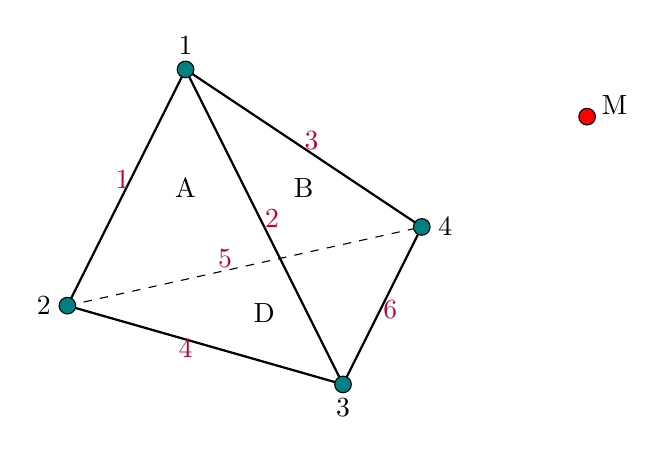
\begin{tikzpicture}
%\draw[step=0.5cm,gray,very thin] (0,0) grid (7,6); 
\draw[thick] (2.5,5) -- (1,2) -- (4.5,1) -- (5.5,3) -- cycle;
\draw[thick] (2.5,5)  -- (4.5,1) ;
\draw[dashed] (1,2) --  (5.5,3);
\node[] at (2.5,5.3) {$1$};
\node[] at (0.7,2) {$2$};
\node[] at (4.5,0.7) {$3$};
\node[] at (5.8,3) {$4$};
\draw[black,fill=teal] (2.5,5) circle (3pt);
\draw[black,fill=teal] (1,2) circle (3pt);
\draw[black,fill=teal] (4.5,1) circle (3pt);
\draw[black,fill=teal] (5.5,3) circle (3pt);
\node[] at (2.5,3.5) {A};
\node[] at (4,3.5) {B};
\node[] at (3.5,1.9) {D};
\draw[black,fill=red] (7.6,4.4) circle (3pt);
\node[] at (7.95,4.55) {M};
\node[] at (1.7,3.6) {\color{purple}1};
\node[] at (3.6,3.1) {\color{purple}2};
\node[] at (4.1,4.1) {\color{purple}3};
\node[] at (2.5,1.45) {\color{purple}4};
\node[] at (3,2.6) {\color{purple}5};
\node[] at (5.1,1.95) {\color{purple}6};
\end{tikzpicture}\\
{\captionfont Face C is hidden in the back.}
\end{center}


When looking at a face from the outside towards the tetrahedron the numbering 
of vertices is counter-clockwise.
\begin{center}
\begin{tabular}{ccccc}
\hline
face & vertices $i,j,k$ & edge \#1 & edge \#2 & edge \#3 \\
\hline\hline
A& 1,2,3  & 12({\color{purple}1}) & 23({\color{purple}4}) & 31({\color{purple}2}) \\
B& 1,3,4  & 13({\color{purple}2}) & 34({\color{purple}6}) & 41({\color{purple}3}) \\
C& 1,4,2  & 14({\color{purple}3}) & 42({\color{purple}5}) & 21({\color{purple}1}) \\
D& 2,4,3  & 24({\color{purple}5}) & 43({\color{purple}6}) & 32({\color{purple}4}) \\
\hline
edge & vertices & belongs to \\
{\color{purple}1} & 12 & A,C\\
{\color{purple}2} & 13 & A,B\\
{\color{purple}3} & 14 & B,C\\
{\color{purple}4} & 23 & A,D\\
{\color{purple}5} & 24 & C,D\\
{\color{purple}6} & 34 & B,D\\
\hline
\end{tabular}
\end{center}


\begin{center}
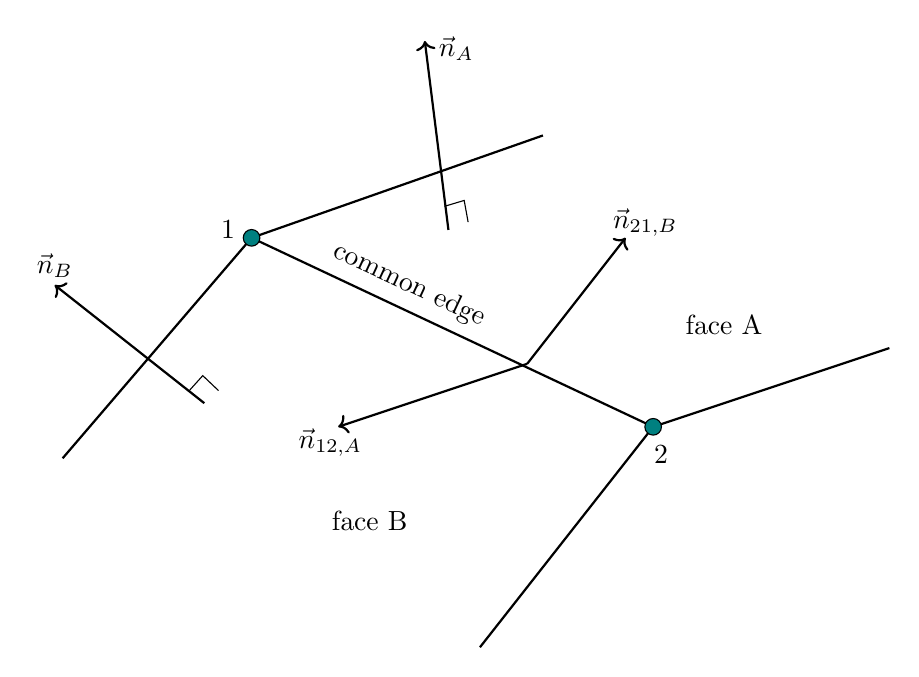
\begin{tikzpicture}
%\draw[step=0.5cm,gray,very thin] (0,0) grid (12,8.5); 
\draw[thick] (0.6,2.8) -- (3,5.6)--(6.7,6.9);
\draw[thick] (3,5.6)  -- (8.1,3.2) ;
\draw[thick] (5.9,0.4) -- (8.1,3.2) -- (11.1,4.2);
\node[] at (9,4.5) {face A};
\node[] at (4.5,2) {face B};
\draw[thick,->] (2.4,3.5)--(0.5,5); 
\node[] at (0.5,5.25) {$\vec{n}_B$};
\draw[] (2.2,3.65) -- (2.38,3.85) --(2.58,3.66);
\draw[thick,->] (5.5,5.7)--(5.2,8.1); 
\node[] at (5.6,8) {$\vec{n}_A$};
\draw[] (5.45,6) --(5.7,6.075) --(5.75,5.8);
\node[] at (2.7,5.7) {1};
\node[] at (8.2,2.85) {2};
\draw[black,fill=teal] (3,5.6) circle (3pt);
\draw[black,fill=teal] (8.1,3.2) circle (3pt);
\node[] at (8,5.8) {$\vec{n}_{21,B}$};
\draw[thick,->] (6.5,4)--(7.75,5.6); 
\node[] at (4,3) {$\vec{n}_{12,A}$};
\draw[thick,->] (6.5,4)--(4.1,3.2); 
\node[rotate=-25] at (5,5) {common edge};
\end{tikzpicture}\\
{\captionfont Figure made after Fig.~7 from \textcite{wesc97}.}
\end{center}



$\vec{n}_{1,A}=\vec{n}_{12,A}=(n_x,n_y)$ is such that it is perpendicular to $\vec{n}_A$ 
(it lies in the face $A$ plane), i.e. $\vec{n}_{1,A}\cdot \vec{n}_A=0$ and to edge $\#1$, i.e. 
$\vec{n}_{1,A}\cdot \vec{l}_{1}=0$. The cross product of $\vec{n}_A$ and $\vec{l}_{1}$ is 
by definition a vector perpendicular to both.
We also need to make sure it is pointing outwards. We then take the scalar product of a 
vector joining the center of the face and the middle of the 
edge under consideration. If it is negative then the normal is pointing towards the center of the 
face so it needs to be flipped.




%-------------------------------------------
\section*{Tetrahedron: Point mass approach}

Let us denote by $V$ the volume of the tetrahedron which 
can easily be computed:
\begin{equation}
V=\frac16 \left| (\vec{l}_{\color{purple}1} \times \vec{l}_{\color{purple}2}) \cdot \vec{l}_{\color{purple}3}\right|
\label{eq:tet:vol}
\end{equation}

\begin{center}
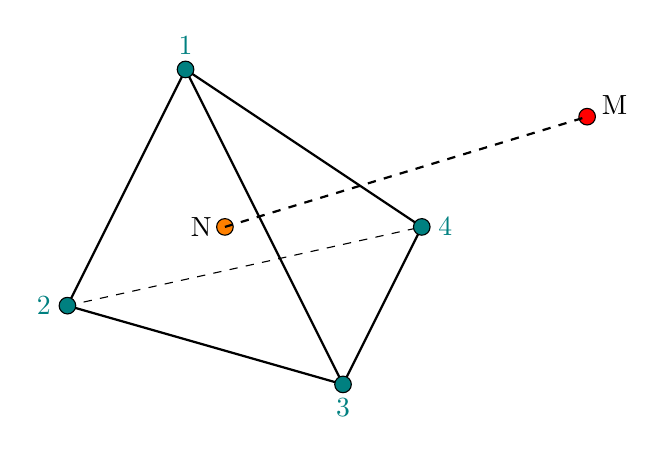
\begin{tikzpicture}
%\draw[step=0.5cm,gray,very thin] (0,0) grid (7,6); 
\draw[thick] (2.5,5) -- (1,2) -- (4.5,1) -- (5.5,3) -- cycle;
\draw[thick] (2.5,5)  -- (4.5,1) ;
\draw[dashed] (1,2) --  (5.5,3);
\node[] at (2.5,5.3) {\color{teal}$1$};
\node[] at (0.7,2) {\color{teal}$2$};
\node[] at (4.5,0.7) {\color{teal}$3$};
\node[] at (5.8,3) {\color{teal}$4$};
\draw[black,fill=teal] (2.5,5) circle (3pt);
\draw[black,fill=teal] (1,2) circle (3pt);
\draw[black,fill=teal] (4.5,1) circle (3pt);
\draw[black,fill=teal] (5.5,3) circle (3pt);

\draw[black,fill=orange] (3,3) circle (3pt);
\node[] at (2.7,3) {N};

\draw[black,fill=red] (7.6,4.4) circle (3pt);
\node[] at (7.95,4.55) {M};

\draw[thick,dashed] (3,3)--(7.6,4.4);

\end{tikzpicture}
\end{center}


The coordinates of its center of gravity $N$ (under the assumption that the 
density is constant inside it) are given by 
\begin{equation}
x_N= \frac{1}{4}(x_{\color{teal}1}+x_{\color{teal}2}+x_{\color{teal}3}+x_{\color{teal}4})
\qquad
y_N= \frac{1}{4}(y_{\color{teal}1}+y_{\color{teal}2}+y_{\color{teal}3}+y_{\color{teal}4})
\qquad
z_N= \frac{1}{4}(z_{\color{teal}1}+z_{\color{teal}2}+z_{\color{teal}3}+z_{\color{teal}4})
\label{eq:tet:centerN}
\end{equation}
If the tetrahedron is considered a point mass, then 
the gravity field and potential are given by
\begin{eqnarray}
\vec{g}_{pm} &=& {\cal G}  \frac{\rho_0 V}{|\overrightarrow{MN}|^3} \overrightarrow{MN}
\\
U_{pm} &=& {\cal G}  \frac{\rho_0 V}{|\overrightarrow{MN}|} 
\end{eqnarray}
with 
\[
\overrightarrow{MN} =
\left(
\begin{array}{c}
x_N - x_M \\
y_N - y_M \\
z_N - z_M 
\end{array}
\right)
\]

Function \verb|compute_gravity_tetrahedron_pointmass| receives coordinates of the four 
vertices {\color{teal}1}, {\color{teal}2}, {\color{teal}3}, {\color{teal}4},  its 
density and the coordinates of the measurement point.

\begin{enumerate}
\item compute coordinates $x_N,y_N,z_N$ of center of gravity with Eq.~\eqref{eq:tet:centerN}
$\rightarrow$ \verb|xN,yN,zN|

\item compute volume $V$ of tetrahedron with Eq.~\eqref{eq:tet:vol}$ \rightarrow$ \verb|Vol| 
\item compute $\vec{g}_{pm}$
\end{enumerate}

%--------------------------------
\section*{Tetrahedron: the algorithm}

Function \verb|compute_gravity_tetrahedron| receives coordinates of the four vertices {\color{teal}1}, 
{\color{teal}2}, {\color{teal}3}, {\color{teal}4}, its density $\rho_0$ and the coordinates of the 
measurement point $M$.

I do not like the notation $\vec{e}_{12}$ for an edge vector since in fieldstone $\vec{e}$ is always 
a unit vector for the coordinate system. I then rename edge vectors $\vec{l}$.

The structure of the function goes as follows:
\begin{enumerate}
\item compute $\vec{l}_{\color{purple}1}$, $\vec{l}_{\color{purple}2}$,etc ... and their norms 
$\rightarrow$ \verb|vec_l1|, \verb|vec_l2|, \verb|vec_l3|, \verb|vec_l4|, \verb|vec_l5|, \verb|vec_l6|

\[
\vec{l}_{\color{purple}1} = \vec{l}_{\color{teal}12} = \left(
\begin{array}{c}
x_{\color{teal}2}-x_{\color{teal}1} \\
y_{\color{teal}2}-y_{\color{teal}1} \\
z_{\color{teal}2}-z_{\color{teal}1}
\end{array}
\right)
\qquad
\vec{l}_{\color{purple}2} = \vec{l}_{\color{teal}13} = \left(
\begin{array}{c}
x_{\color{teal}3}-x_{\color{teal}1} \\
y_{\color{teal}3}-y_{\color{teal}1} \\
z_{\color{teal}3}-z_{\color{teal}1}
\end{array}
\right)
\qquad
\textrm{etc...}
\]


\item compute $\vec{r}_{\color{teal} 1,2,3,4}$. $\rightarrow$ \verb|vec_r1|, \verb|vec_r2|, \verb|vec_r3|, \verb|vec_r4|
\[
\vec{r}_{\color{teal}1} = \vec{M1} = \left(
\begin{array}{c}
x_{\color{teal}1}-x_m \\
y_{\color{teal}1}-y_m \\
z_{\color{teal}1}-z_m
\end{array}
\right)
\]



\item compute $\vec{n}_{A,B,C,D}$. 
$\rightarrow$ \verb|vec_nA| , \verb|vec_nB|, \verb|vec_nC|, \verb|vec_nD|

\begin{eqnarray}
\vec{n}_A 
&=& \vec{l}_{\color{teal}12}\times\vec{l}_{\color{teal}13}/|\vec{l}_{\color{teal}12}\times\vec{l}_{\color{teal}13}|
= \vec{l}_{\color{purple}1}\times\vec{l}_{\color{purple}2}/| \vec{l}_{\color{purple}1}\times\vec{l}_{\color{purple}2}| \\
\vec{n}_B 
&=& \vec{l}_{\color{teal}13}\times\vec{l}_{\color{teal}14}/|\vec{l}_{\color{teal}13}\times\vec{l}_{\color{teal}14}|
= \vec{l}_{\color{purple}2}\times\vec{l}_{\color{purple}3}/|\vec{l}_{\color{purple}2}\times\vec{l}_{\color{purple}3}|  \\
\vec{n}_C 
&=& \vec{l}_{\color{teal}14}\times\vec{l}_{\color{teal}12}/|\vec{l}_{\color{teal}14}\times\vec{l}_{\color{teal}12}|   
= \vec{l}_{\color{purple}3}\times\vec{l}_{\color{purple}1}/|\vec{l}_{\color{purple}3}\times\vec{l}_{\color{purple}1}|   \\
\vec{n}_D 
&=& \vec{l}_{\color{teal}24}\times\vec{l}_{\color{teal}23}/|\vec{l}_{\color{teal}24}\times\vec{l}_{\color{teal}23}|   
= \vec{l}_{\color{purple}5}\times\vec{l}_{\color{purple}4}/|\vec{l}_{\color{purple}5}\times\vec{l}_{\color{purple}4}|
\end{eqnarray}


\item compute ${\bm F}_{A,B,C,D}$. 
$\rightarrow$ \verb|mat_FA| , \verb|mat_FB|, \verb|mat_FC|, 
\verb|mat_FD|

\begin{eqnarray}
{\bm F}_A &=& \vec{n}_A\vec{n}_A \\
{\bm F}_B &=& \vec{n}_B\vec{n}_B \\
{\bm F}_C &=& \vec{n}_C\vec{n}_C \\
{\bm F}_D &=& \vec{n}_D\vec{n}_D 
\end{eqnarray}

\item compute $\omega_{A,B,C,D}$. $\rightarrow$ \verb|wA| , \verb|wB|, \verb|wC|, \verb|wD|

\begin{eqnarray}
\omega_A &=& 
2 \arctan \frac{\vec{r_{\color{teal}1}} \cdot (\vec{r}_{\color{teal}2} \times \vec{r}_{\color{teal}3})}{r_{\color{teal}1}r_{\color{teal}2}r_{\color{teal}3} 
+{r}_{\color{teal}1}(\vec{r}_{\color{teal}2}\cdot\vec{r}_{\color{teal}3}) 
+{r}_{\color{teal}2}(\vec{r}_{\color{teal}3}\cdot\vec{r}_{\color{teal}1}) 
+{r}_{\color{teal}3}(\vec{r}_{\color{teal}1}\cdot\vec{r}_{\color{teal}2})  } \nn\\
\omega_B &=& 
2 \arctan \frac{\vec{r_{\color{teal}1}} \cdot (\vec{r}_{\color{teal}3} \times \vec{r}_{\color{teal}4})}{r_{\color{teal}1}r_{\color{teal}3}r_{\color{teal}4} 
+r_{\color{teal}1}(\vec{r}_{\color{teal}3}\cdot\vec{r}_{\color{teal}4}) 
+r_{\color{teal}3}(\vec{r}_{\color{teal}4}\cdot\vec{r}_{\color{teal}1}) 
+r_{\color{teal}4}(\vec{r}_{\color{teal}1}\cdot\vec{r}_{\color{teal}3})  } \nn\\
\omega_C &=&
2 \arctan \frac{\vec{r_{\color{teal}1}} \cdot (\vec{r}_{\color{teal}4} \times \vec{r}_{\color{teal}2})}{r_{\color{teal}1}r_{\color{teal}4}r_{\color{teal}2}
+r_{\color{teal}1}(\vec{r}_{\color{teal}4}\cdot\vec{r}_{\color{teal}2}) 
+r_{\color{teal}4}(\vec{r}_{\color{teal}2}\cdot\vec{r}_{\color{teal}1}) 
+r_{\color{teal}2}(\vec{r}_{\color{teal}1}\cdot\vec{r}_{\color{teal}4}) 
} \nn\\
\omega_D &=&
2 \arctan \frac{\vec{r_{\color{teal}2}} \cdot (\vec{r}_{\color{teal}4} \times \vec{r}_{\color{teal}3})}{r_{\color{teal}2}r_{\color{teal}4}r_{\color{teal}3} 
+r_{\color{teal}2}(\vec{r}_{\color{teal}4}\cdot\vec{r}_{\color{teal}3}) 
+r_{\color{teal}4}(\vec{r}_{\color{teal}3}\cdot\vec{r}_{\color{teal}2}) 
+r_{\color{teal}3}(\vec{r}_{\color{teal}2}\cdot\vec{r}_{\color{teal}4}) 
}
\end{eqnarray}

which translates into
\begin{lstlisting}
num=np.dot(vec_r1,np.cross(vec_r2,vec_r3))
denom=(r1*r2*r3+\
       r1*np.dot(vec_r2,vec_r3)+\
       r2*np.dot(vec_r3,vec_r1)+\
       r3*np.dot(vec_r1,vec_r2))
wA=2*np.arctan2(num,denom)
\end{lstlisting}


\item compute $\vec{r}_{A}$, $\vec{r}_{B}$, $\vec{r}_{C}$, $\vec{r}_{D}$.
As explained in the caption of their Figure~3, ``vector $\vec{r}_f$
extends from the field point $M$ to any point in the face plane''.
$\rightarrow$ \verb|vec_rA|, \verb|vec_rB|, \verb|vec_rC|, \verb|vec_rD|

\item compute $\vec{g}_f$ by means of % Eq.~\eqref{eq:tetra:gf}

\[
\vec{g}_f
= {\cal G} \rho_0 \sum_f \omega_f {\bm F}_f\cdot \vec{r}_f 
= {\cal G} \rho_0 \left(
\omega_A {\bm F}_A\cdot \vec{r}_A +
\omega_B {\bm F}_B\cdot \vec{r}_B +
\omega_C {\bm F}_C\cdot \vec{r}_C +
\omega_D {\bm F}_D\cdot \vec{r}_D 
\right)
\]




\item compute $\vec{n}_{e,f}$ for each edge of each face (12 vectors!)
$\rightarrow$ \verb|vec_nA12|, \verb|vec_nA23|, \verb|vec_nA13|, \verb|vec_nB13|, etc ...


\item compute ${\bm E}_{\color{purple} 1,2,3,4,5,6}$. 
$\rightarrow$ \verb|mat_E12, mat_E13, mat_E14, mat_E23, mat_E24, mat_E34| 

\begin{eqnarray}
{\bm E}_{\color{purple}1} ={\bm E}_{\color{teal}12}
&=&\vec{n}_A \vec{n}_{{\color{teal}12},A} +\vec{n}_C \vec{n}_{{\color{teal}21},C}\\
{\bm E}_{\color{purple}2} ={\bm E}_{\color{teal}13}
&=& \vec{n}_A \vec{n}_{{\color{teal}13},A} +\vec{n}_B \vec{n}_{{\color{teal}13},B} \\
{\bm E}_{\color{purple}3} ={\bm E}_{\color{teal}14}
&=& \vec{n}_B \vec{n}_{{\color{teal}14},B}+\vec{n}_C \vec{n}_{{\color{teal}14},C} \\
{\bm E}_{\color{purple}4} ={\bm E}_{\color{teal}23}
&=& \vec{n}_A \vec{n}_{{\color{teal}23},A}+\vec{n}_D \vec{n}_{{\color{teal}23},D} \\
{\bm E}_{\color{purple}5} ={\bm E}_{\color{teal}24}
&=& \vec{n}_C \vec{n}_{{\color{teal}24},C} +\vec{n}_D \vec{n}_{{\color{teal}24},D} \\  
{\bm E}_{\color{purple}6} ={\bm E}_{\color{teal}34}
&=& \vec{n}_B \vec{n}_{{\color{teal}34},B} +\vec{n}_D \vec{n}_{{\color{teal}34},D} 
\end{eqnarray}



\item compute $L_{\color{purple}1,2,3,4,5,6}$ $\rightarrow$ \verb|L12|, \verb|L13|, \verb|L14|, ...
\begin{eqnarray}
L_{\color{purple}1} = L_{\color{teal}12} 
&=& \ln \frac{r_{\color{teal}1}+r_{\color{teal}2}+l_{\color{purple}1}}{r_{\color{teal}1}+r_{\color{teal}2}-l_{\color{purple}1}} \nn\\
L_{\color{purple}2} = L_{\color{teal}13} 
&=& \ln \frac{r_{\color{teal}1}+r_{\color{teal}3}+l_{\color{purple}2}}{r_{\color{teal}1}+r_{\color{teal}3}-l_{\color{purple}2}} \nn\\
L_{\color{purple}3} = L_{\color{teal}14} 
&=& \ln \frac{r_{\color{teal}1}+r_{\color{teal}4}+l_{\color{purple}3}}{r_{\color{teal}1}+r_{\color{teal}4}-l_{\color{purple}3}} \nn\\
L_{\color{purple}4} = L_{\color{teal}23} 
&=& \ln \frac{r_{\color{teal}2}+r_{\color{teal}3}+l_{\color{purple}4}}{r_{\color{teal}2}+r_{\color{teal}3}-l_{\color{purple}4}} \nn\\
L_{\color{purple}5} = L_{\color{teal}24} 
&=& \ln \frac{r_{\color{teal}2}+r_{\color{teal}4}+l_{\color{purple}5}}{r_{\color{teal}2}+r_{\color{teal}4}-l_{\color{purple}5}} \nn\\
L_{\color{purple}6} = L_{\color{teal}34} 
&=& \ln \frac{r_{\color{teal}3}+r_{\color{teal}4}+l_{\color{purple}6}}{r_{\color{teal}3}+r_{\color{teal}4}-l_{\color{purple}6}} \nn
\end{eqnarray}


\item compute $\vec{r}_{\color{teal}12,13,14,23,24,34}$. As specified in Section~2.1.8 of their 
paper ``$\vec{r}_e$ is a vector from the field point to any point on edge $e$ or its infinite extension''
$\rightarrow$ \verb|vec_r12|, \verb|vec_r13|, \verb|vec_r13|, etc ...  


\item compute $\vec{g}_e$ by means of Eq.~\eqref{eq:tetra:ge}

\begin{eqnarray}
\vec{g}_e 
&=&{\cal G} \rho_0 \sum_e L_e {\bm E}_e \cdot \vec{r}_e \nn\\
&=&{\cal G} \rho_0 \left( 
L_{\color{teal}12} {\bm E}_{\color{teal}12}\cdot\vec{r}_{\color{teal}12} +
L_{\color{teal}13} {\bm E}_{\color{teal}23}\cdot\vec{r}_{\color{teal}13} +
L_{\color{teal}14} {\bm E}_{\color{teal}34}\cdot\vec{r}_{\color{teal}14} +
L_{\color{teal}23} {\bm E}_{\color{teal}23}\cdot\vec{r}_{\color{teal}23} + 
L_{\color{teal}24} {\bm E}_{\color{teal}24}\cdot\vec{r}_{\color{teal}24} +
L_{\color{teal}34} {\bm E}_{\color{teal}34}\cdot\vec{r}_{\color{teal}34} 
\right)
\end{eqnarray}


\item compute $\vec{g}=-\vec{g}_e+\vec{g}_f$

\end{enumerate}

Except for the 4 measurements provided in \textcite{mequ86} I could not easily find 
actual values to benchmark the code against, so the following three examples aim at 
remedying this problem. 
In all what follows we set $\rho_0=1$ and ${\cal G}=1$ for simplicity.

%..............................................
\section*{Tetrahedron test 1: the Wikipedia tetrahedron}

We consider the following regular tetrahedron (i.e. all faces are equilateral triangles) centered at the 
origin\footnote{\url{https://en.wikipedia.org/wiki/Tetrahedron}}. Its edges are $l=\sqrt{8/3}$ long.
We have
\begin{eqnarray}
(x_1,y_1,z_1) &=& (0,0,1) \nn\\
(x_2,y_2,z_2) &=& (\sqrt{8/9},0,-1/3) \nn\\
(x_3,y_3,z_3) &=& (-\sqrt{2/9},\sqrt{2/3},-1/3) \nn\\
(x_4,y_4,z_4) &=& (-\sqrt{2/9},-\sqrt{2/3},-1/3) \nn
\end{eqnarray}
Point 1 is at the top and points 2,3,4 are in the $z=-1/3$ plane.

\begin{center}
\includegraphics[width=5cm]{python_codes/fieldstone_113/images/tet1}
\includegraphics[width=4cm]{python_codes/fieldstone_113/results/test1/tet}
\end{center}

The volume of a regular tetrahedron of edge $l$ is given by:
\[
V=\frac{l^3}{6\sqrt{2}} = \frac{8}{9\sqrt{3}} \simeq 0.5132
\]
and this is what we indeed recover.

\begin{lstlisting}
pt_meas = np.array([0,0,10],dtype=np.float64)
pt_one=np.array([0,0,1],dtype=np.float64)
pt_two=np.array([-np.sqrt(2/9),-np.sqrt(2/3),-1/3],dtype=np.float64)
pt_three=np.array([np.sqrt(8/9),0,-1/3],dtype=np.float64)
pt_four=np.array([-np.sqrt(2/9),np.sqrt(2/3),-1/3],dtype=np.float64)
\end{lstlisting}

\begin{center}
\includegraphics[width=8cm]{python_codes/fieldstone_113/results/test1/g_vector.pdf}
\includegraphics[width=8cm]{python_codes/fieldstone_113/results/test1/g_vector_diff.pdf}\\
\includegraphics[width=8cm]{python_codes/fieldstone_113/results/test1/g_pot.pdf}
\includegraphics[width=8cm]{python_codes/fieldstone_113/results/test1/g_pot_diff.pdf}
\end{center}

%..............................................
\section*{Tetrahedron test 2: the 111-tetrahedron}

It is defined in \textcite{mequ86} (1986) (with a correction by \textcite{camq86} (1986)).

\begin{center}
\includegraphics[width=8cm]{python_codes/fieldstone_113/images/mequ86a}
\end{center}

\begin{lstlisting}
alpha=1.
pt_meas = np.array([2,0.5,0.5],dtype=np.float64)
pt_one=np.array([alpha,alpha,alpha],dtype=np.float64)
pt_two=np.array([alpha,0,0],dtype=np.float64)
pt_three=np.array([0,alpha,0],dtype=np.float64)
pt_four=np.array([0,0,alpha],dtype=np.float64)
\end{lstlisting}


In this case I choose pt1 is node C, pt2 is H, pt3 is F pt 4 is A.
If the cube is a unit cube then the edge length is $\sqrt{2}$ and the volume
\[
V=\frac{l^3}{6\sqrt{2}} = \frac13
\]

\begin{center}
\includegraphics[width=5cm]{python_codes/fieldstone_113/images/tet2}
\end{center}

\textcite{mequ86} state: ``To ensure that the above analysis can be treated
with confidence we have performed numerical calculations of the field components Fx, Fy, and 
Fz using the expressions developed in this paper and
have compared them with those obtained by direct numerical integration'':
\begin{center}
\includegraphics[width=7cm]{python_codes/fieldstone_113/images/mequ86b}\\
{\captionfont Taken from \textcite{mequ86}.}
\end{center}

\begin{center}
\begin{tabular}{lllcc}
\hline
$x$ & $y$ & $z$ & $g_x$ (tet) & $g_x$ (point mass) \\
\hline
\hline
1.25 & 0.5 & 0.5 &  0.566679144260546  & 0.5925925925925926 \\
1.5  & 0.5 & 0.5 &  0.326526930616740  & 0.3333333333333333 \\
1.75 & 0.5 & 0.5 &  0.211222015971550  & 0.2133333333333333 \\
2.0  & 0.5 & 0.5 &  0.147377525744174  & 0.1481481481481481 \\
\hline
\end{tabular}\\
Results obtained with this \stone.
\end{center}

Gravity fields are measured on a line starting at $(1,0.456,0.567)$ and ending at $(5,0.456,0.567)$
\begin{center}
\includegraphics[width=8cm]{python_codes/fieldstone_113/results/test2/g_vector.pdf}
\includegraphics[width=8cm]{python_codes/fieldstone_113/results/test2/g_vector_diff.pdf}\\
\includegraphics[width=8cm]{python_codes/fieldstone_113/results/test2/g_pot.pdf}
\includegraphics[width=8cm]{python_codes/fieldstone_113/results/test2/g_pot_diff.pdf}
\end{center}


%..........................................
\section*{Tetrahedron test 3: the origin tetrahedron}

This is not a regular tetrahedron since $l_{1} \neq l_4 $.

\begin{center}
\includegraphics[width=5cm]{python_codes/fieldstone_113/images/tet3}
\end{center}


\begin{eqnarray}
(x_1,y_1,z_1) &=& (0,0,0) \nn\\
(x_2,y_2,z_2) &=& (1,0,0) \nn\\ 
(x_3,y_3,z_3) &=& (0,1,0) \nn\\
(x_4,y_4,z_4) &=& (0,0,1) \nn
\end{eqnarray}

The gravity fields are measured on a line starting at $(1,1,1)$ and ending at $(3,3,3)$:

\begin{center}
\includegraphics[width=7cm]{python_codes/fieldstone_113/results/test3/g_vector.pdf}
\includegraphics[width=7cm]{python_codes/fieldstone_113/results/test3/g_vector_diff.pdf}\\
\includegraphics[width=7cm]{python_codes/fieldstone_113/results/test3/g_pot.pdf}
\includegraphics[width=7cm]{python_codes/fieldstone_113/results/test3/g_pot_diff.pdf}
\end{center}


%.................................................
\section*{Tetrahedron test 4: cube containing 5 tetrahedra}

{\color{red} to do!}


\newpage
%===============================================================
\section*{Hexahedron: theory}


In what follows $e={\color{purple} 1,2,3,...}$ stands for an edge while $f=A,B,C,...$ stands for a face. 
Each polyhedron face has an outward-pointing face normal vector $\vec{n}_f$
and a face dyad ${\bm F}_f =\vec{n}_f\vec{n}_f $.
Each edge of each face has an outward-pointing edge normal
vector $\vec{n}_{e,f}$ perpendicular to both $\vec{n}_f$ and the edge.
For the edge connecting vertices 1 and 2 shared by faces A and B,
the edge dyad is ${\bm E}_{12}=\vec{n}_A \vec{n}_{12,A}+\vec{n}_B \vec{n}_{21,B}$.

Let $\vec{r}_i$ represent the vector from the variable 
field-point M at location $\vec{r}_M$ to polyhedron vertex $P_i$, 
and let $r_i = ||\vec{r}_i||$ be its length.


For the polyhedron edge connecting
vertices $i$ and $j$ of length $l_{ij}$, the dimensionless per-edge factor $L_e$ is
\[
L_e=L_{ij} = \int_e \frac{1}{r}ds = \int_{P_i}^{P_j} \frac{1}{r} ds 
= \ln \frac{r_i+r_j+l_{ij}}{r_i+r_j-l_{ij}}
\]
For a triangular face $f$ bounded by vertices $i,j,k$ the dimensionless
per-face factor $\omega_f$ is  
\[
\omega_f = 
\iint_{triangle} \frac{\Delta z}{r^3} dS 
= 2 \arctan \frac{\vec{r_i} \cdot (\vec{r}_j \times \vec{r}_k)}{r_ir_jr_k 
+r_i(\vec{r}_j\cdot\vec{r}_k) 
+r_j(\vec{r}_k\cdot\vec{r}_i) 
+r_k(\vec{r}_i\cdot\vec{r}_j) 
}
\]

\begin{center}
\includegraphics[width=5cm]{python_codes/fieldstone_113/images/hex1}
\includegraphics[width=5cm]{python_codes/fieldstone_113/images/hex2}\\
{\captionfont Left: unit cube; Right: triangles making up the visible faces.}
\end{center}



When looking at a face from the outside towards the tetrahedron the numbering 
of vertices is counter-clockwise.
\begin{center}
\begin{tabular}{ccccc}
\hline
face & vertices $i,j,k$ & edge \#1 & edge \#2 & edge \#3 \\
\hline\hline
A& 5,1,6 & 5-1 ({\color{purple}9})  & 1-6 ({\color{purple}13})  & 6-5 ({\color{purple}1})  \\
B& 2,6,1 & 2-6 ({\color{purple}10}) & 6-1 ({\color{purple}13})  & 1-2 ({\color{purple}5})  \\
C& 6,2,7 & 6-2 ({\color{purple}10}) & 2-7 ({\color{purple}14})  & 7-6 ({\color{purple}2})  \\
D& 3,7,2 & 3-7 ({\color{purple}11}) & 7-2 ({\color{purple}14})  & 2-3 ({\color{purple}6})  \\
E& 3,4,7 & 3-4 ({\color{purple}7})  & 4-7 ({\color{purple}15})  & 7-3 ({\color{purple}11}) \\
F& 8,7,4 & 8-7 ({\color{purple}3})  & 7-4 ({\color{purple}15})  & 4-8 ({\color{purple}12}) \\
G& 8,4,5 & 8-4 ({\color{purple}12}) & 4-5 ({\color{purple}16})  & 5-8 ({\color{purple}4})  \\
H& 1,5,4 & 1-5 ({\color{purple}9})  & 5-4 ({\color{purple}16})  & 4-1 ({\color{purple}8})  \\
I& 7,8,6 & 7-8 ({\color{purple}3})  & 8-6 ({\color{purple}17})  & 6-7 ({\color{purple}2})  \\
J& 5,6,8 & 5-6 ({\color{purple}1})  & 6-8 ({\color{purple}17})  & 8-5 ({\color{purple}4})  \\
K& 4,3,1 & 4-3 ({\color{purple}7})  & 3-1 ({\color{purple}18})  & 1-4 ({\color{purple}8})  \\
L& 2,1,3 & 2-1 ({\color{purple}5})  & 1-3 ({\color{purple}18})  & 3-2 ({\color{purple}6})  \\
\hline
\end{tabular}
\end{center}


%===============================================================
\section*{Hexahedron: algorithm}

\begin{enumerate}

%.....................................................................................................
\item compute $\vec{l}_{\color{purple}1}$, $\vec{l}_{\color{purple}2}$,etc ... and their norms
$\rightarrow$ \verb|vec_l01|, \verb|vec_l02|, \verb|vec_l03|, \verb|vec_l04|, ... \verb|vec_l18|

\[
\vec{l}_{\color{purple}1} = \vec{l}_{\color{teal}56} = \left(
\begin{array}{c}
x_{\color{teal}6}-x_{\color{teal}5} \\
y_{\color{teal}6}-y_{\color{teal}5} \\
z_{\color{teal}6}-z_{\color{teal}5}
\end{array}
\right)
\qquad
\vec{l}_{\color{purple}2} = \vec{l}_{\color{teal}67} = \left(
\begin{array}{c}
x_{\color{teal}7}-x_{\color{teal}6} \\
y_{\color{teal}7}-y_{\color{teal}6} \\
z_{\color{teal}7}-z_{\color{teal}6}
\end{array}
\right)
\qquad
\textrm{etc...}
\]

{\tiny
\begin{lstlisting}
    vec_l01=np.zeros(3,dtype=np.float64) ; vec_l01 = pt_5-pt_6 ; l01 = LA.norm(vec_l01,2)
    vec_l02=np.zeros(3,dtype=np.float64) ; vec_l02 = pt_6-pt_7 ; l02 = LA.norm(vec_l02,2)
    vec_l03=np.zeros(3,dtype=np.float64) ; vec_l03 = pt_7-pt_8 ; l03 = LA.norm(vec_l03,2)
    ...
    vec_l16=np.zeros(3,dtype=np.float64) ; vec_l16 = pt_4-pt_5 ; l16 = LA.norm(vec_l16,2)
    vec_l17=np.zeros(3,dtype=np.float64) ; vec_l17 = pt_6-pt_8 ; l17 = LA.norm(vec_l17,2)
    vec_l18=np.zeros(3,dtype=np.float64) ; vec_l18 = pt_1-pt_3 ; l18 = LA.norm(vec_l18,2)
\end{lstlisting}
}

%.................................................................................................
\item compute $\vec{r}_{\color{teal} 1,2,3,4,5,6,7,8}$. $\rightarrow$ \verb|vec_r01|, \verb|vec_r02|, \verb|vec_r03|, ... \verb|vec_r08|.
For example:
\[
\vec{r}_{\color{teal}1} = \vec{M1} = \left(
\begin{array}{c}
x_{\color{teal}1}-x_m \\
y_{\color{teal}1}-y_m \\
z_{\color{teal}1}-z_m
\end{array}
\right)
\qquad\qquad
r_{\color{teal}1}= |\vec{r}_{\color{teal}1}|
\]

{\tiny
\begin{lstlisting}
    vec_r01=np.zeros(3,dtype=np.float64) ; vec_r01 = pt_1-pt_M ; r01=LA.norm(vec_r01,2)
    vec_r02=np.zeros(3,dtype=np.float64) ; vec_r02 = pt_2-pt_M ; r02=LA.norm(vec_r02,2)
    vec_r03=np.zeros(3,dtype=np.float64) ; vec_r03 = pt_3-pt_M ; r03=LA.norm(vec_r03,2)
    vec_r04=np.zeros(3,dtype=np.float64) ; vec_r04 = pt_4-pt_M ; r04=LA.norm(vec_r04,2)
    vec_r05=np.zeros(3,dtype=np.float64) ; vec_r05 = pt_5-pt_M ; r05=LA.norm(vec_r05,2)
    vec_r06=np.zeros(3,dtype=np.float64) ; vec_r06 = pt_6-pt_M ; r06=LA.norm(vec_r06,2)
    vec_r07=np.zeros(3,dtype=np.float64) ; vec_r07 = pt_7-pt_M ; r07=LA.norm(vec_r07,2)
    vec_r08=np.zeros(3,dtype=np.float64) ; vec_r08 = pt_8-pt_M ; r08=LA.norm(vec_r08,2)

    r01=LA.norm(vec_r01,2)
    r02=LA.norm(vec_r02,2)
    r03=LA.norm(vec_r03,2)
    r04=LA.norm(vec_r04,2)
    r05=LA.norm(vec_r05,2)
    r06=LA.norm(vec_r06,2)
    r07=LA.norm(vec_r07,2)
    r08=LA.norm(vec_r08,2)
\end{lstlisting}
}


%.................................................................................................
\item compute $\vec{n}_{A,B,C,D,...K,L}$ and coordinates of face centers. 
$\rightarrow$ \verb|vec_nA| , \verb|vec_nB|, \verb|vec_nC|, \verb|vec_nD|, ... \verb|vec_nK|, \verb|vec_nL|

\begin{eqnarray}
\vec{n}_A 
&=& \vec{l}_{\color{teal}51}\times\vec{l}_{\color{teal}56}/
   |\vec{l}_{\color{teal}51}\times\vec{l}_{\color{teal}56}|
= -\vec{l}_{\color{purple}9}\times\vec{l}_{\color{purple}1}/
| -\vec{l}_{\color{purple}9}\times\vec{l}_{\color{purple}1}| 
\nn\\
\vec{n}_B 
&=& \vec{l}_{\color{teal}26}\times\vec{l}_{\color{teal}21}/
   |\vec{l}_{\color{teal}26}\times\vec{l}_{\color{teal}21}|
= \vec{l}_{\color{purple}10}\times-\vec{l}_{\color{purple}5}/
 |\vec{l}_{\color{purple}10}\times-\vec{l}_{\color{purple}5}|  
\nn\\
\vec{n}_C 
&=& \vec{l}_{\color{teal}62}\times\vec{l}_{\color{teal}67}/
   |\vec{l}_{\color{teal}62}\times\vec{l}_{\color{teal}67}|   
= -\vec{l}_{\color{purple}10}\times\vec{l}_{\color{purple}2}/
 |-\vec{l}_{\color{purple}10}\times\vec{l}_{\color{purple}2}| 
\nn  \\
\vec{n}_D 
&=& \vec{l}_{\color{teal}37}\times\vec{l}_{\color{teal}32}/
   |\vec{l}_{\color{teal}37}\times\vec{l}_{\color{teal}32}|   
= \vec{l}_{\color{purple}11}\times-\vec{l}_{\color{purple}6}/
 |\vec{l}_{\color{purple}11}\times-\vec{l}_{\color{purple}6}|
\nn\\
\vec{n}_E
&=& \vec{l}_{\color{teal}34}\times\vec{l}_{\color{teal}37}/
   |\vec{l}_{\color{teal}34}\times\vec{l}_{\color{teal}37}|   
= \vec{l}_{\color{purple}7}\times\vec{l}_{\color{purple}11}/
 |\vec{l}_{\color{purple}7}\times\vec{l}_{\color{purple}11}|
\nn\\
\vec{n}_F
&=& \vec{l}_{\color{teal}87}\times\vec{l}_{\color{teal}84}/
   |\vec{l}_{\color{teal}87}\times\vec{l}_{\color{teal}84}|   
= -\vec{l}_{\color{purple}3}\times-\vec{l}_{\color{purple}12}/
 |-\vec{l}_{\color{purple}3}\times-\vec{l}_{\color{purple}12}|
\nn\\
\vec{n}_G
&=& \vec{l}_{\color{teal}84}\times\vec{l}_{\color{teal}85}/
   |\vec{l}_{\color{teal}84}\times\vec{l}_{\color{teal}85}|   
= -\vec{l}_{\color{purple}12}\times\vec{l}_{\color{purple}4}/
 |-\vec{l}_{\color{purple}12}\times\vec{l}_{\color{purple}4}|
\nn\\
\vec{n}_H
&=& \vec{l}_{\color{teal}15}\times\vec{l}_{\color{teal}14}/
   |\vec{l}_{\color{teal}14}\times\vec{l}_{\color{teal}14}|   
= \vec{l}_{\color{purple}9}\times-\vec{l}_{\color{purple}8}/
 |\vec{l}_{\color{purple}9}\times-\vec{l}_{\color{purple}8}|
\nn\\
\vec{n}_I
&=& \vec{l}_{\color{teal}78}\times\vec{l}_{\color{teal}76}/
   |\vec{l}_{\color{teal}78}\times\vec{l}_{\color{teal}76}|   
= \vec{l}_{\color{purple}3}\times-\vec{l}_{\color{purple}2}/
 |\vec{l}_{\color{purple}3}\times-\vec{l}_{\color{purple}2}|
\nn\\
\vec{n}_J
&=& \vec{l}_{\color{teal}56}\times\vec{l}_{\color{teal}58}/
   |\vec{l}_{\color{teal}56}\times\vec{l}_{\color{teal}58}|   
= \vec{l}_{\color{purple}1}\times-\vec{l}_{\color{purple}4}/
 |\vec{l}_{\color{purple}1}\times-\vec{l}_{\color{purple}4}|
\nn\\
\vec{n}_K
&=& \vec{l}_{\color{teal}43}\times\vec{l}_{\color{teal}41}/
   |\vec{l}_{\color{teal}43}\times\vec{l}_{\color{teal}41}|   
= -\vec{l}_{\color{purple}7}\times\vec{l}_{\color{purple}8}/
 |-\vec{l}_{\color{purple}7}\times\vec{l}_{\color{purple}8}|
\nn\\
\vec{n}_L
&=& \vec{l}_{\color{teal}21}\times\vec{l}_{\color{teal}23}/
   |\vec{l}_{\color{teal}21}\times\vec{l}_{\color{teal}23}|   
= -\vec{l}_{\color{purple}5}\times\vec{l}_{\color{purple}6}/
 |-\vec{l}_{\color{purple}5}\times\vec{l}_{\color{purple}6}|
\nn
\end{eqnarray}

{\tiny
\begin{lstlisting}
pt_midA=np.zeros(3,dtype=np.float64) ; pt_midA = (pt_1+pt_6+pt_5)/3
pt_midB=np.zeros(3,dtype=np.float64) ; pt_midB = (pt_1+pt_2+pt_6)/3
pt_midC=np.zeros(3,dtype=np.float64) ; pt_midC = (pt_2+pt_7+pt_6)/3 
...
pt_midJ=np.zeros(3,dtype=np.float64) ; pt_midJ = (pt_8+pt_5+pt_6)/3
pt_midK=np.zeros(3,dtype=np.float64) ; pt_midK = (pt_3+pt_1+pt_4)/3
pt_midL=np.zeros(3,dtype=np.float64) ; pt_midL = (pt_3+pt_2+pt_1)/3

vec_nA=np.zeros(3,dtype=np.float64) ; vec_nA = np.cross( vec_l13, vec_l09) ; vec_nA/=LA.norm(vec_nA,2)
vec_nB=np.zeros(3,dtype=np.float64) ; vec_nB = np.cross( vec_l10,-vec_l05) ; vec_nB/=LA.norm(vec_nB,2)
vec_nC=np.zeros(3,dtype=np.float64) ; vec_nC = np.cross(-vec_l10, vec_l02) ; vec_nC/=LA.norm(vec_nC,2)
...
vec_nJ=np.zeros(3,dtype=np.float64) ; vec_nJ = np.cross( vec_l01,-vec_l04) ; vec_nJ/=LA.norm(vec_nJ,2)
vec_nK=np.zeros(3,dtype=np.float64) ; vec_nK = np.cross(-vec_l07, vec_l08) ; vec_nK/=LA.norm(vec_nK,2)
vec_nL=np.zeros(3,dtype=np.float64) ; vec_nL = np.cross(-vec_l05, vec_l06) ; vec_nL/=LA.norm(vec_nL,2)
\end{lstlisting}
}




%.....................................................................................
\item compute ${\bm F}_{A,B,C,D}$. 
$\rightarrow$ \verb|mat_FaceA| , \verb|mat_FaceB|, \verb|mat_FaceC|, 
\verb|mat_FaceD|, ... \verb|mat_FaceL|

\begin{eqnarray}
{\bm F}_A &=& \vec{n}_A\vec{n}_A \nn\\
{\bm F}_B &=& \vec{n}_B\vec{n}_B \nn\\
{\bm F}_C &=& \vec{n}_C\vec{n}_C \nn\\
... \nn\\
{\bm F}_K &=& \vec{n}_K\vec{n}_K \nn\\
{\bm F}_L &=& \vec{n}_L\vec{n}_L \nn
\end{eqnarray}

{\tiny
\begin{lstlisting}
mat_FA=np.zeros((3,3),dtype=np.float64) ; mat_FA=np.outer(vec_nA,vec_nA)
mat_FB=np.zeros((3,3),dtype=np.float64) ; mat_FB=np.outer(vec_nB,vec_nB)
mat_FC=np.zeros((3,3),dtype=np.float64) ; mat_FC=np.outer(vec_nC,vec_nC)
...
mat_FJ=np.zeros((3,3),dtype=np.float64) ; mat_FJ=np.outer(vec_nJ,vec_nJ)
mat_FK=np.zeros((3,3),dtype=np.float64) ; mat_FK=np.outer(vec_nK,vec_nK)
mat_FL=np.zeros((3,3),dtype=np.float64) ; mat_FL=np.outer(vec_nL,vec_nL)
\end{lstlisting}
}

%............................................................................................
\item compute $\omega_{A,B,C,D}$. $\rightarrow$ \verb|wA|, \verb|wB|, \verb|wC|, \verb|wD|, ... \verb|wK|, \verb|wL|.
In what follows $r_i=|\vec{r}_i|$.


\begin{eqnarray}
\omega_A &=& 
2 \arctan \frac{\vec{r_{\color{teal}5}} \cdot (\vec{r}_{\color{teal}1} \times \vec{r}_{\color{teal}6})}
{{r}_{\color{teal}5}{r}_{\color{teal}1}{r}_{\color{teal}6} 
+{r}_{\color{teal}1}(\vec{r}_{\color{teal}6}\cdot\vec{r}_{\color{teal}5}) 
+{r}_{\color{teal}6}(\vec{r}_{\color{teal}5}\cdot\vec{r}_{\color{teal}1}) 
+{r}_{\color{teal}5}(\vec{r}_{\color{teal}1}\cdot\vec{r}_{\color{teal}6})  }  
\qquad A=\{{\color{teal}5,1,6}\}=\{ {\color{purple} 9,13,1} \}
\nn\\
\omega_B &=& 
2 \arctan \frac{\vec{r_{\color{teal}2}} \cdot (\vec{r}_{\color{teal}6} \times \vec{r}_{\color{teal}1})}
{{r}_{\color{teal}2}{r}_{\color{teal}6}{r}_{\color{teal}1} 
+{r}_{\color{teal}1}(\vec{r}_{\color{teal}2}\cdot\vec{r}_{\color{teal}6}) 
+{r}_{\color{teal}2}(\vec{r}_{\color{teal}6}\cdot\vec{r}_{\color{teal}1}) 
+{r}_{\color{teal}6}(\vec{r}_{\color{teal}1}\cdot\vec{r}_{\color{teal}2})  }  
\qquad B=\{ {\color{teal}2,6,1} \}=\{ {\color{purple} 10,13,5} \}
\nn\\
\omega_C &=& 
2 \arctan \frac{\vec{r_{\color{teal}6}} \cdot (\vec{r}_{\color{teal}2} \times \vec{r}_{\color{teal}7})}
{{r}_{\color{teal}6}{r}_{\color{teal}2}{r}_{\color{teal}7} 
+{r}_{\color{teal}2}(\vec{r}_{\color{teal}7}\cdot\vec{r}_{\color{teal}6}) 
+{r}_{\color{teal}7}(\vec{r}_{\color{teal}6}\cdot\vec{r}_{\color{teal}2}) 
+{r}_{\color{teal}6}(\vec{r}_{\color{teal}2}\cdot\vec{r}_{\color{teal}7})  }  
\qquad C=\{ {\color{teal}6,2,7} \}=\{ {\color{purple} 10,14,2} \}
\nn\\
\omega_D &=& 
2 \arctan \frac{\vec{r_{\color{teal}3}} \cdot (\vec{r}_{\color{teal}7} \times \vec{r}_{\color{teal}2})}
{{r}_{\color{teal}3}{r}_{\color{teal}7}{r}_{\color{teal}2} 
+{r}_{\color{teal}2}(\vec{r}_{\color{teal}3}\cdot\vec{r}_{\color{teal}7}) 
+{r}_{\color{teal}3}(\vec{r}_{\color{teal}7}\cdot\vec{r}_{\color{teal}2}) 
+{r}_{\color{teal}7}(\vec{r}_{\color{teal}2}\cdot\vec{r}_{\color{teal}3})  }  
\qquad D=\{ {\color{teal}3,7,2} \}=\{ {\color{purple} 11,14,6} \}
\nn\\
\omega_E &=& 
2 \arctan \frac{\vec{r_{\color{teal}3}} \cdot (\vec{r}_{\color{teal}4} \times \vec{r}_{\color{teal}7})}
{{r}_{\color{teal}3}{r}_{\color{teal}4}{r}_{\color{teal}7} 
+{r}_{\color{teal}1}(\vec{r}_{\color{teal}6}\cdot\vec{r}_{\color{teal}5}) 
+{r}_{\color{teal}6}(\vec{r}_{\color{teal}5}\cdot\vec{r}_{\color{teal}1}) 
+{r}_{\color{teal}5}(\vec{r}_{\color{teal}1}\cdot\vec{r}_{\color{teal}6})  }  
\qquad E=\{ {\color{teal} 3,4,7} \}=\{ {\color{purple} 7,15,11} \}
\nn\\
\omega_F &=& 
2 \arctan \frac{\vec{r_{\color{teal}8}} \cdot (\vec{r}_{\color{teal}7} \times \vec{r}_{\color{teal}4})}
{{r}_{\color{teal}8}{r}_{\color{teal}7}{r}_{\color{teal}4} 
+{r}_{\color{teal}7}(\vec{r}_{\color{teal}4}\cdot\vec{r}_{\color{teal}8}) 
+{r}_{\color{teal}4}(\vec{r}_{\color{teal}8}\cdot\vec{r}_{\color{teal}7}) 
+{r}_{\color{teal}8}(\vec{r}_{\color{teal}7}\cdot\vec{r}_{\color{teal}4})  }  
\qquad F=\{ {\color{teal} 8,7,4} \}=\{ {\color{purple} 3,15,12} \}
\nn\\
\omega_G &=& 
2 \arctan \frac{\vec{r_{\color{teal}8}} \cdot (\vec{r}_{\color{teal}4} \times \vec{r}_{\color{teal}5})}
{{r}_{\color{teal}8}{r}_{\color{teal}4}{r}_{\color{teal}5} 
+{r}_{\color{teal}4}(\vec{r}_{\color{teal}5}\cdot\vec{r}_{\color{teal}8}) 
+{r}_{\color{teal}5}(\vec{r}_{\color{teal}8}\cdot\vec{r}_{\color{teal}4}) 
+{r}_{\color{teal}8}(\vec{r}_{\color{teal}4}\cdot\vec{r}_{\color{teal}5})  }  
\qquad G=\{ {\color{teal}8,4,5} \}=\{ {\color{purple} 12,16,4} \}
\nn\\
\omega_H &=& 
2 \arctan \frac{\vec{r_{\color{teal}1}} \cdot (\vec{r}_{\color{teal}5} \times \vec{r}_{\color{teal}4})}
{{r}_{\color{teal}1}{r}_{\color{teal}5}{r}_{\color{teal}4} 
+{r}_{\color{teal}4}(\vec{r}_{\color{teal}1}\cdot\vec{r}_{\color{teal}5}) 
+{r}_{\color{teal}1}(\vec{r}_{\color{teal}5}\cdot\vec{r}_{\color{teal}4}) 
+{r}_{\color{teal}5}(\vec{r}_{\color{teal}4}\cdot\vec{r}_{\color{teal}1})  }  
\qquad H=\{ {\color{teal}1,5,4} \}=\{ {\color{purple} 9,16,8} \}
\nn\\
\omega_I &=& 
2 \arctan \frac{\vec{r_{\color{teal}7}} \cdot (\vec{r}_{\color{teal}8} \times \vec{r}_{\color{teal}6})}
{{r}_{\color{teal}7}{r}_{\color{teal}8}{r}_{\color{teal}6} 
+{r}_{\color{teal}8}(\vec{r}_{\color{teal}6}\cdot\vec{r}_{\color{teal}7}) 
+{r}_{\color{teal}6}(\vec{r}_{\color{teal}7}\cdot\vec{r}_{\color{teal}8}) 
+{r}_{\color{teal}7}(\vec{r}_{\color{teal}8}\cdot\vec{r}_{\color{teal}6})  }  
\qquad I=\{ {\color{teal}7,8,6}\}=\{ {\color{purple} 3,17,2} \}
\nn\\
\omega_J &=& 
2 \arctan \frac{\vec{r_{\color{teal}5}} \cdot (\vec{r}_{\color{teal}6} \times \vec{r}_{\color{teal}8})}
{{r}_{\color{teal}5}{r}_{\color{teal}6}{r}_{\color{teal}8} 
+{r}_{\color{teal}8}(\vec{r}_{\color{teal}5}\cdot\vec{r}_{\color{teal}6}) 
+{r}_{\color{teal}5}(\vec{r}_{\color{teal}6}\cdot\vec{r}_{\color{teal}8}) 
+{r}_{\color{teal}6}(\vec{r}_{\color{teal}8}\cdot\vec{r}_{\color{teal}5})  }  
\qquad J=\{ {\color{teal}5,6,8}\}=\{ {\color{purple} 1,17,4} \}
\nn\\
\omega_K &=& 
2 \arctan \frac{\vec{r_{\color{teal}4}} \cdot (\vec{r}_{\color{teal}3} \times \vec{r}_{\color{teal}1})}
{{r}_{\color{teal}4}{r}_{\color{teal}3}{r}_{\color{teal}1} 
+{r}_{\color{teal}3}(\vec{r}_{\color{teal}1}\cdot\vec{r}_{\color{teal}4}) 
+{r}_{\color{teal}1}(\vec{r}_{\color{teal}4}\cdot\vec{r}_{\color{teal}3}) 
+{r}_{\color{teal}4}(\vec{r}_{\color{teal}3}\cdot\vec{r}_{\color{teal}1})  }  
\qquad K=\{{\color{teal}4,3,1}\}=\{ {\color{purple} 7,18,8} \}
\nn\\
\omega_L &=& 
2 \arctan \frac{\vec{r_{\color{teal}2}} \cdot (\vec{r}_{\color{teal}1} \times \vec{r}_{\color{teal}3})}
{{r}_{\color{teal}2}{r}_{\color{teal}1}{r}_{\color{teal}3} 
+{r}_{\color{teal}3}(\vec{r}_{\color{teal}2}\cdot\vec{r}_{\color{teal}1}) 
+{r}_{\color{teal}2}(\vec{r}_{\color{teal}1}\cdot\vec{r}_{\color{teal}3}) 
+{r}_{\color{teal}1}(\vec{r}_{\color{teal}3}\cdot\vec{r}_{\color{teal}2})  }  
\qquad L=\{ {\color{teal}2,1,3}\}=\{ {\color{purple} 5,18,6} \}
\nn
\end{eqnarray}



{\tiny
\begin{lstlisting}
num=np.dot(vec_r5,np.cross(vec_r1,vec_r6))
denom=(r05*r01*r06+r1*np.dot(vec_r06,vec_r05)+r2*np.dot(vec_r03,vec_r01)+r3*np.dot(vec_r01,vec_r02))
wA=2*np.arctan2(num,denom)
\end{lstlisting}
}




%..........................................................................................step6
\item compute $\vec{r}_{A}$, $\vec{r}_{B}$, $\vec{r}_{C}$, $\vec{r}_{D}$.
As explained in the caption of their Figure~3, ``vector $\vec{r}_f$
extends from the field point $M$ to any point in the face plane''.
$\rightarrow$ \verb|vec_rA|, \verb|vec_rB|, \verb|vec_rC|, \verb|vec_rD|, ... \verb|ver_rL|

{\tiny
\begin{lstlisting}
    vec_rA = pt_midA-pt_M
    vec_rB = pt_midB-pt_M
    vec_rC = pt_midC-pt_M
    vec_rD = pt_midD-pt_M
    vec_rE = pt_midE-pt_M
    vec_rF = pt_midF-pt_M
    vec_rG = pt_midG-pt_M
    vec_rH = pt_midH-pt_M
    vec_rI = pt_midI-pt_M
    vec_rJ = pt_midJ-pt_M
    vec_rK = pt_midK-pt_M
    vec_rL = pt_midL-pt_M
\end{lstlisting}
}




%...........................................................................................step7
\item compute $\vec{g}_f$ by means of % Eq.~\eqref{eq:tetra:gf}

\[
\vec{g}_f
= {\cal G} \rho_0 \sum_f \omega_f {\bm F}_f\cdot \vec{r}_f 
= {\cal G} \rho_0 \left(
\omega_A {\bm F}_A\cdot \vec{r}_A +
\omega_B {\bm F}_B\cdot \vec{r}_B +
\omega_C {\bm F}_C\cdot \vec{r}_C +
\omega_D {\bm F}_D\cdot \vec{r}_D +
...+
\omega_L {\bm F}_L \cdot \vec{r}_L
\right)
\]

{\tiny
\begin{lstlisting}
    vec_gf=np.zeros(3,dtype=np.float64)
    vec_gf=wA*np.dot(mat_FA,vec_rA) +\
           wB*np.dot(mat_FB,vec_rB) +\
           wC*np.dot(mat_FC,vec_rC) +\
           wD*np.dot(mat_FD,vec_rD) +\
           wE*np.dot(mat_FE,vec_rE) +\
           wF*np.dot(mat_FF,vec_rF) +\
           wG*np.dot(mat_FG,vec_rG) +\
           wH*np.dot(mat_FH,vec_rH) +\
           wI*np.dot(mat_FI,vec_rI) +\
           wJ*np.dot(mat_FJ,vec_rJ) +\
           wK*np.dot(mat_FK,vec_rK) +\
           wL*np.dot(mat_FL,vec_rL)
    vec_gf*=Ggrav*rho0
\end{lstlisting}
}


%.........................................................................................step8
\item compute $\vec{n}_{e,f}$ for each edge of each face (12 triangles*3=36 vectors!)
$\rightarrow$ \verb|vec_nA12|, \verb|vec_nA23|, \verb|vec_nA13|, \verb|vec_nB13|, etc ...

{\tiny
\begin{lstlisting}
    vec_nA12 = compute_face_edge_normal(vec_nA,pt_1,pt_2,pt_midA,'faceA_n12')
    vec_nA23 = compute_face_edge_normal(vec_nA,pt_2,pt_3,pt_midA,'faceA_n23')
    vec_nA13 = compute_face_edge_normal(vec_nA,pt_3,pt_1,pt_midA,'faceA_n31')
\end{lstlisting}
}




%.........................................................................................step9
\item compute ${\bm E}_{\color{purple} 1,2,3,4,5,6,...18}$.
$\rightarrow$ \verb|mat_E12, mat_E13, mat_E14, mat_E23, mat_E24, mat_E34|.
For the edge connecting vertices 1 and 2 shared by faces A and B,
the edge dyad is ${\bm E}_{12}=\vec{n}_A \vec{n}_{12,A}+\vec{n}_B \vec{n}_{21,B}$.


\begin{center}
\begin{tabular}{ccccc}
\hline
edge & vertices & belongs to \\
{\color{purple}1}  & 5,6 & J,A\\
{\color{purple}2}  & 6,7 & I,C\\
{\color{purple}3}  & 7,8 & I,F\\
{\color{purple}4}  & 8,5 & J,G\\
{\color{purple}5}  & 1,2 & B,L\\
{\color{purple}6}  & 2,3 & D,L\\
{\color{purple}7}  & 3,4 & E,K\\
{\color{purple}8}  & 4,1 & H,K\\
{\color{purple}9}  & 1,5 & H,A\\
{\color{purple}10} & 2,6 & B,C \\
{\color{purple}11} & 3,7 & D,E\\
{\color{purple}12} & 4,8 & F,G\\
{\color{purple}13} & 1,6 & A,B\\
{\color{purple}14} & 2,7 & C,D\\
{\color{purple}15} & 4,7 & E,F\\
{\color{purple}16} & 4,5 & G,H\\
{\color{purple}17} & 6,8 & J,I\\
{\color{purple}18} & 1,3 & L,K\\
\hline
\end{tabular}
\end{center}
The first letter is the face left of the arrow, the second letter is the face right of the arrow.

\begin{center}
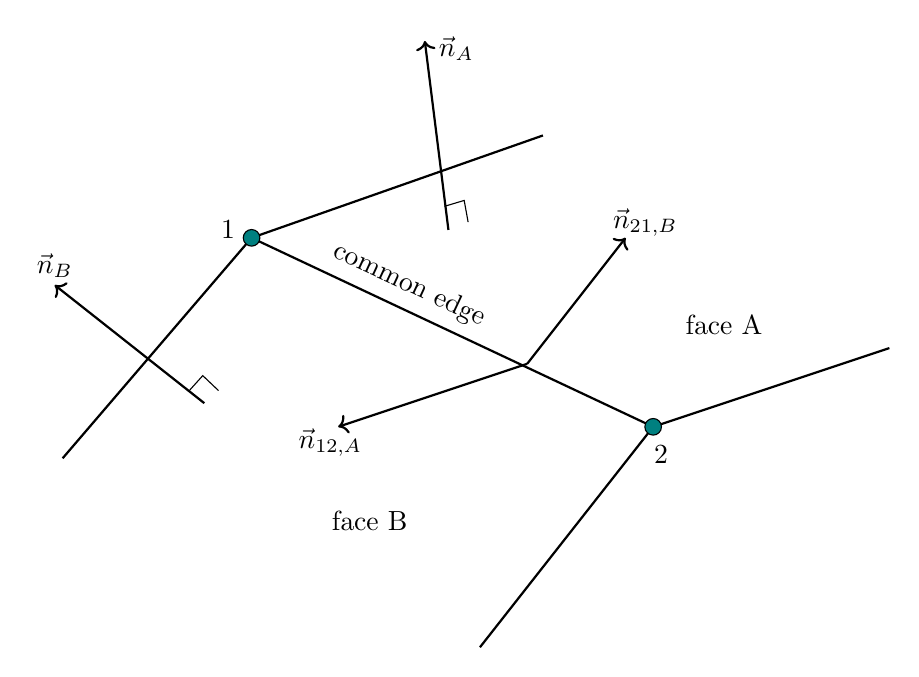
\begin{tikzpicture}
%\draw[step=0.5cm,gray,very thin] (0,0) grid (12,8.5); 
\draw[thick] (0.6,2.8) -- (3,5.6)--(6.7,6.9);
\draw[thick] (3,5.6)  -- (8.1,3.2) ;
\draw[thick] (5.9,0.4) -- (8.1,3.2) -- (11.1,4.2);
\node[] at (9,4.5) {face A}; 
\node[] at (4.5,2) {face B}; 
\draw[thick,->] (2.4,3.5)--(0.5,5); 
\node[] at (0.5,5.25) {$\vec{n}_B$};
\draw[] (2.2,3.65) -- (2.38,3.85) --(2.58,3.66);
\draw[thick,->] (5.5,5.7)--(5.2,8.1); 
\node[] at (5.6,8) {$\vec{n}_A$};
\draw[] (5.45,6) --(5.7,6.075) --(5.75,5.8);
\node[] at (2.7,5.7) {1};
\node[] at (8.2,2.85) {2};
\draw[black,fill=teal] (3,5.6) circle (3pt);
\draw[black,fill=teal] (8.1,3.2) circle (3pt);
\node[] at (8,5.8) {$\vec{n}_{21,B}$};
\draw[thick,->] (6.5,4)--(7.75,5.6); 
\node[] at (4,3) {$\vec{n}_{12,A}$};
\draw[thick,->] (6.5,4)--(4.1,3.2); 
\node[rotate=-25] at (5,5) {common edge};
\end{tikzpicture}\\
{\captionfont Figure made after Fig.~7 from \textcite{wesc97}.}
\end{center}


\begin{eqnarray}
{\bm E}_{\color{purple}1} ={\bm E}_{\color{teal}56}
&=&\vec{n}_A \vec{n}_{{\color{teal}12},A} 
+  \vec{n}_J \vec{n}_{{\color{teal}21},J} \nn\\
{\bm E}_{\color{purple}2} ={\bm E}_{\color{teal}67}
&=&\vec{n}_I \vec{n}_{{\color{teal}13},I} 
+  \vec{n}_C \vec{n}_{{\color{teal}13},C} \nn\\
{\bm E}_{\color{purple}3} ={\bm E}_{\color{teal}78}
&=&\vec{n}_F \vec{n}_{{\color{teal}14},F}
+  \vec{n}_I \vec{n}_{{\color{teal}14},I} \nn\\
{\bm E}_{\color{purple}4} ={\bm E}_{\color{teal}85}
&=&\vec{n}_J \vec{n}_{{\color{teal}23},J}
+  \vec{n}_G \vec{n}_{{\color{teal}23},G} \nn\\
{\bm E}_{\color{purple}5} ={\bm E}_{\color{teal}12}
&=&\vec{n}_B \vec{n}_{{\color{teal}24},B} 
+  \vec{n}_L \vec{n}_{{\color{teal}24},L} \nn\\  
{\bm E}_{\color{purple}6} ={\bm E}_{\color{teal}23}
&=&\vec{n}_L \vec{n}_{{\color{teal}34},L} 
+  \vec{n}_D \vec{n}_{{\color{teal}34},D} \nn\\
{\bm E}_{\color{purple}7} ={\bm E}_{\color{teal}34}  
&=&\vec{n}_E \vec{n}_{{\color{teal}34},E} 
+  \vec{n}_K \vec{n}_{{\color{teal}34},K} \nn\\
{\bm E}_{\color{purple}8} ={\bm E}_{\color{teal}41}  
&=&\vec{n}_H \vec{n}_{{\color{teal}34},H} 
+  \vec{n}_K \vec{n}_{{\color{teal}34},K} \nn\\
{\bm E}_{\color{purple}9} ={\bm E}_{\color{teal}15}  
&=&\vec{n}_A \vec{n}_{{\color{teal}34},A} 
+  \vec{n}_H \vec{n}_{{\color{teal}34},H} \nn\\
{\bm E}_{\color{purple}10} ={\bm E}_{\color{teal}26} 
&=&\vec{n}_B \vec{n}_{{\color{teal}34},B} 
+  \vec{n}_C \vec{n}_{{\color{teal}34},C} \nn\\
{\bm E}_{\color{purple}11} ={\bm E}_{\color{teal}37} 
&=&\vec{n}_D \vec{n}_{{\color{teal}34},D} 
+  \vec{n}_E \vec{n}_{{\color{teal}34},E} \nn\\
{\bm E}_{\color{purple}12} ={\bm E}_{\color{teal}48} 
&=&\vec{n}_F \vec{n}_{{\color{teal}34},F} 
+  \vec{n}_G \vec{n}_{{\color{teal}34},G} \nn\\
{\bm E}_{\color{purple}13} ={\bm E}_{\color{teal}16}   
&=&\vec{n}_A \vec{n}_{{\color{teal}34},A} 
+  \vec{n}_B \vec{n}_{{\color{teal}34},B} \nn\\
{\bm E}_{\color{purple}14} ={\bm E}_{\color{teal}27}   
&=&\vec{n}_C \vec{n}_{{\color{teal}34},C} 
+  \vec{n}_D \vec{n}_{{\color{teal}34},D} \nn\\
{\bm E}_{\color{purple}15} ={\bm E}_{\color{teal}47}   
&=&\vec{n}_E \vec{n}_{{\color{teal}47},E} 
+  \vec{n}_F \vec{n}_{{\color{teal}74},F} \nn\\
{\bm E}_{\color{purple}16} ={\bm E}_{\color{teal}45}   
&=&\vec{n}_G \vec{n}_{{\color{teal}45},G} 
+  \vec{n}_H \vec{n}_{{\color{teal}54},H} \nn\\
{\bm E}_{\color{purple}17} ={\bm E}_{\color{teal}68}   
&=&\vec{n}_I \vec{n}_{{\color{teal}68},I} 
+  \vec{n}_J \vec{n}_{{\color{teal}86},J} \nn\\
{\bm E}_{\color{purple}18} ={\bm E}_{\color{teal}13} 
&=&\vec{n}_K \vec{n}_{{\color{teal}13},K} 
+  \vec{n}_L \vec{n}_{{\color{teal}31},L} \nn
\end{eqnarray}

{\tiny
\begin{lstlisting}
mat_E56=np.outer(vec_nJ,vec_nJ56)+np.outer(vec_nA,vec_nA65) #edge 5-6 ( 1) belongs to J & A
mat_E67=np.outer(vec_nI,vec_nI67)+np.outer(vec_nC,vec_nC76) #edge 6-7 ( 2) belongs to I & C
mat_E78=np.outer(vec_nI,vec_nI78)+np.outer(vec_nF,vec_nF87) #edge 7-8 ( 3) belongs to I & F
mat_E85=np.outer(vec_nJ,vec_nJ85)+np.outer(vec_nG,vec_nG58) #edge 8-5 ( 4) belongs to J & G
mat_E12=np.outer(vec_nB,vec_nB12)+np.outer(vec_nL,vec_nL21) #edge 1-2 ( 5) belongs to B & L
mat_E23=np.outer(vec_nD,vec_nD23)+np.outer(vec_nL,vec_nL32) #edge 2-3 ( 6) belongs to D & L
mat_E34=np.outer(vec_nE,vec_nE34)+np.outer(vec_nK,vec_nK43) #edge 3-4 ( 7) belongs to E & K 
mat_E41=np.outer(vec_nH,vec_nH41)+np.outer(vec_nK,vec_nK14) #edge 4-1 ( 8) belongs to H & K
mat_E15=np.outer(vec_nH,vec_nH15)+np.outer(vec_nA,vec_nA51) #edge 1-5 ( 9) belongs to H & A
mat_E26=np.outer(vec_nB,vec_nB26)+np.outer(vec_nC,vec_nC62) #edge 2-6 (10) belongs to B & C
mat_E37=np.outer(vec_nD,vec_nD37)+np.outer(vec_nE,vec_nE73) #edge 3-7 (11) belongs to D & E
mat_E48=np.outer(vec_nF,vec_nF48)+np.outer(vec_nG,vec_nG84) #edge 4-8 (12) belongs to F & G
mat_E16=np.outer(vec_nA,vec_nA16)+np.outer(vec_nB,vec_nB61) #edge 1-6 (13) belongs to A & B
mat_E27=np.outer(vec_nC,vec_nC27)+np.outer(vec_nD,vec_nD72) #edge 2-7 (14) belongs to C & D
mat_E47=np.outer(vec_nE,vec_nE47)+np.outer(vec_nF,vec_nF74) #edge 4-7 (15) belongs to E & F
mat_E45=np.outer(vec_nG,vec_nG45)+np.outer(vec_nH,vec_nH54) #edge 4-5 (16) belongs to G & H
mat_E68=np.outer(vec_nJ,vec_nJ68)+np.outer(vec_nI,vec_nI86) #edge 6-8 (17) belongs to J & I
mat_E13=np.outer(vec_nL,vec_nL13)+np.outer(vec_nK,vec_nK31) #edge 1-3 (18) belongs to L & K
\end{lstlisting}
}


%..................................................................................... step 10
\item compute $L_{\color{purple}1,2,3,4,5,6}$ $\rightarrow$ \verb|L01|, \verb|L02|, \verb|L03|, ... 
\begin{eqnarray}
L_{\color{purple}1} = L_{\color{teal}56} 
&=& \ln \frac{r_{\color{teal}5}+r_{\color{teal}6}+l_{\color{purple}1}}
             {r_{\color{teal}5}+r_{\color{teal}6}-l_{\color{purple}1}} 
\nn\\
L_{\color{purple}2} = L_{\color{teal}67} 
&=& \ln \frac{r_{\color{teal}6}+r_{\color{teal}7}+l_{\color{purple}2}}
             {r_{\color{teal}6}+r_{\color{teal}7}-l_{\color{purple}2}} 
\nn\\
L_{\color{purple}3} = L_{\color{teal}78} 
&=& \ln \frac{r_{\color{teal}7}+r_{\color{teal}8}+l_{\color{purple}3}}
             {r_{\color{teal}7}+r_{\color{teal}8}-l_{\color{purple}3}} 
\nn\\
L_{\color{purple}4} = L_{\color{teal}85} 
&=& \ln \frac{r_{\color{teal}8}+r_{\color{teal}5}+l_{\color{purple}4}}
             {r_{\color{teal}8}+r_{\color{teal}5}-l_{\color{purple}4}} 
\nn\\
L_{\color{purple}5} = L_{\color{teal}12} 
&=& \ln \frac{r_{\color{teal}1}+r_{\color{teal}2}+l_{\color{purple}5}}
             {r_{\color{teal}1}+r_{\color{teal}2}-l_{\color{purple}5}} 
\nn\\
L_{\color{purple}6} = L_{\color{teal}23} 
&=& \ln \frac{r_{\color{teal}2}+r_{\color{teal}3}+l_{\color{purple}6}}
             {r_{\color{teal}2}+r_{\color{teal}3}-l_{\color{purple}6}} 
\nn\\
L_{\color{purple}7} = L_{\color{teal}34} 
&=& \ln \frac{r_{\color{teal}3}+r_{\color{teal}4}+l_{\color{purple}7}}
             {r_{\color{teal}3}+r_{\color{teal}4}-l_{\color{purple}7}} 
\nn\\
L_{\color{purple}8} = L_{\color{teal}41} 
&=& \ln \frac{r_{\color{teal}4}+r_{\color{teal}3}+l_{\color{purple}8}}
             {r_{\color{teal}4}+r_{\color{teal}3}-l_{\color{purple}8}} 
\nn\\
L_{\color{purple}9} = L_{\color{teal}15} 
&=& \ln \frac{r_{\color{teal}1}+r_{\color{teal}5}+l_{\color{purple}9}}
             {r_{\color{teal}1}+r_{\color{teal}5}-l_{\color{purple}9}} 
\nn\\
L_{\color{purple}10} = L_{\color{teal}26} 
&=& \ln \frac{r_{\color{teal}2}+r_{\color{teal}6}+l_{\color{purple}10}}
             {r_{\color{teal}2}+r_{\color{teal}6}-l_{\color{purple}10}} 
\nn\\
L_{\color{purple}11} = L_{\color{teal}37} 
&=& \ln \frac{r_{\color{teal}3}+r_{\color{teal}7}+l_{\color{purple}11}}
             {r_{\color{teal}3}+r_{\color{teal}7}-l_{\color{purple}11}} 
\nn\\
L_{\color{purple}12} = L_{\color{teal}48} 
&=& \ln \frac{r_{\color{teal}4}+r_{\color{teal}8}+l_{\color{purple}12}}
             {r_{\color{teal}4}+r_{\color{teal}8}-l_{\color{purple}12}} 
\nn\\
L_{\color{purple}13} = L_{\color{teal}16} 
&=& \ln \frac{r_{\color{teal}1}+r_{\color{teal}6}+l_{\color{purple}13}}
             {r_{\color{teal}1}+r_{\color{teal}6}-l_{\color{purple}13}} 
\nn\\
L_{\color{purple}14} = L_{\color{teal}27} 
&=& \ln \frac{r_{\color{teal}2}+r_{\color{teal}7}+l_{\color{purple}14}}
             {r_{\color{teal}2}+r_{\color{teal}7}-l_{\color{purple}14}} 
\nn\\
L_{\color{purple}15} = L_{\color{teal}47} 
&=& \ln \frac{r_{\color{teal}4}+r_{\color{teal}7}+l_{\color{purple}15}}
             {r_{\color{teal}4}+r_{\color{teal}7}-l_{\color{purple}15}} 
\nn\\
L_{\color{purple}16} = L_{\color{teal}45} 
&=& \ln \frac{r_{\color{teal}4}+r_{\color{teal}5}+l_{\color{purple}16}}
             {r_{\color{teal}4}+r_{\color{teal}5}-l_{\color{purple}16}} 
\nn\\
L_{\color{purple}17} = L_{\color{teal}68} 
&=& \ln \frac{r_{\color{teal}6}+r_{\color{teal}8}+l_{\color{purple}17}}
             {r_{\color{teal}6}+r_{\color{teal}8}-l_{\color{purple}17}} 
\nn\\
L_{\color{purple}18} = L_{\color{teal}13} 
&=& \ln \frac{r_{\color{teal}1}+r_{\color{teal}3}+l_{\color{purple}18}}
             {r_{\color{teal}1}+r_{\color{teal}3}-l_{\color{purple}18}} 
\nn
\end{eqnarray}

{\tiny
\begin{lstlisting}
    L01=np.log((r05+r06+l01)/(r05+r06-l01)) #56 
    L02=np.log((r06+r07+l02)/(r06+r07-l02)) #67 
    L03=np.log((r07+r08+l03)/(r07+r08-l03)) #78 
    L04=np.log((r08+r05+l04)/(r08+r05-l04)) #85 
    L05=np.log((r01+r02+l05)/(r01+r02-l05)) #12 
    L06=np.log((r02+r03+l06)/(r02+r03-l06)) #23 
    L07=np.log((r03+r04+l07)/(r03+r04-l07)) #34 
    L08=np.log((r04+r01+l08)/(r04+r01-l08)) #41 
    L09=np.log((r01+r05+l09)/(r01+r05-l09)) #15 
    L10=np.log((r02+r06+l10)/(r02+r06-l10)) #26 
    L11=np.log((r03+r07+l11)/(r03+r07-l11)) #37 
    L12=np.log((r04+r08+l12)/(r04+r08-l12)) #48 
    L13=np.log((r01+r06+l13)/(r01+r06-l13)) #16 
    L14=np.log((r02+r07+l14)/(r02+r07-l14)) #27 
    L15=np.log((r04+r07+l15)/(r04+r07-l15)) #47 
    L16=np.log((r04+r05+l16)/(r04+r05-l16)) #45 
    L17=np.log((r06+r08+l17)/(r06+r08-l17)) #68 
    L18=np.log((r01+r03+l18)/(r01+r03-l18)) #13 
\end{lstlisting}
}


%........................................................................................
\item compute $\vec{r}_{\color{teal}12,13,14,23,24,34}$. As specified in Section~2.1.8 of their
paper ``$\vec{r}_e$ is a vector from the field point to any point on edge $e$ or its infinite extension''. I choose the middle of the edge. $\rightarrow$ \verb|vec_r01|, \verb|vec_r02|, \verb|vec_r03|, etc ...
{\tiny
\begin{lstlisting}
    vec_r01=np.zeros(3,dtype=np.float64) ; vec_r01 = 0.5*(pt_5+pt_6)-pt_M #56 
    vec_r02=np.zeros(3,dtype=np.float64) ; vec_r02 = 0.5*(pt_6+pt_7)-pt_M #67
    vec_r03=np.zeros(3,dtype=np.float64) ; vec_r03 = 0.5*(pt_7+pt_8)-pt_M #78
    vec_r04=np.zeros(3,dtype=np.float64) ; vec_r04 = 0.5*(pt_8+pt_5)-pt_M #85
    vec_r05=np.zeros(3,dtype=np.float64) ; vec_r05 = 0.5*(pt_1+pt_2)-pt_M #12
    vec_r06=np.zeros(3,dtype=np.float64) ; vec_r06 = 0.5*(pt_2+pt_3)-pt_M #23
    vec_r07=np.zeros(3,dtype=np.float64) ; vec_r07 = 0.5*(pt_3+pt_4)-pt_M #34
    vec_r08=np.zeros(3,dtype=np.float64) ; vec_r08 = 0.5*(pt_4+pt_1)-pt_M #41
    vec_r09=np.zeros(3,dtype=np.float64) ; vec_r09 = 0.5*(pt_1+pt_5)-pt_M #15
    vec_r10=np.zeros(3,dtype=np.float64) ; vec_r10 = 0.5*(pt_2+pt_6)-pt_M #26
    vec_r11=np.zeros(3,dtype=np.float64) ; vec_r11 = 0.5*(pt_3+pt_7)-pt_M #37
    vec_r12=np.zeros(3,dtype=np.float64) ; vec_r12 = 0.5*(pt_4+pt_8)-pt_M #48
    vec_r13=np.zeros(3,dtype=np.float64) ; vec_r13 = 0.5*(pt_1+pt_6)-pt_M #16
    vec_r14=np.zeros(3,dtype=np.float64) ; vec_r14 = 0.5*(pt_2+pt_7)-pt_M #27
    vec_r15=np.zeros(3,dtype=np.float64) ; vec_r15 = 0.5*(pt_4+pt_7)-pt_M #47
    vec_r16=np.zeros(3,dtype=np.float64) ; vec_r16 = 0.5*(pt_4+pt_5)-pt_M #45
    vec_r17=np.zeros(3,dtype=np.float64) ; vec_r17 = 0.5*(pt_6+pt_8)-pt_M #68
    vec_r18=np.zeros(3,dtype=np.float64) ; vec_r18 = 0.5*(pt_1+pt_3)-pt_M #13
\end{lstlisting}
}




\item compute $\vec{g}_e$ by means of Eq.~\eqref{eq:tetra:ge}

\[
\vec{g}_e 
={\cal G} \rho_0 \sum_e L_e {\bm E}_e \cdot \vec{r}_e 
={\cal G} \rho_0 \left( 
L_{\color{purple}1} {\bm E}_{\color{purple}1}\cdot\vec{r}_{\color{purple}1} +
L_{\color{purple}2} {\bm E}_{\color{purple}2}\cdot\vec{r}_{\color{purple}2} +
...
L_{\color{purple}17} {\bm E}_{\color{purple}17}\cdot\vec{r}_{\color{purple}17} +
L_{\color{purple}18} {\bm E}_{\color{purple}18}\cdot\vec{r}_{\color{purple}18} 
\right)
\]


\item compute $U_e$ by means of Eq.~\eqref{eq:tetra:Ue}


\item compute $\vec{g}=-\vec{g}_e+\vec{g}_f$

\end{enumerate}



%===============================================================
\section*{Hexahedron: mascons}

The volume of the quadrilateral is computed and since its density is 
constant each mascon has the same mass. 
The number of mascons is $n^3$ and the mascons are spanning the entire 
quadrilateral by means of a linear mapping. They are evenly spread in the 
reference cube $[-1,1]^3$ and then mapped to the real hexahedron.
This is all happening in the function {\python compute\_gravity\_hexahedron\_mascons}.
There is however a problem with this approach. Each mascon is assigned the same mass, 
which is fine if they are all equidistant. They are equidistant in the $r,s,t$ space
but not necessarily in the $x,y,z$ after the mapping, especially if the sides of the 
hexahedron are not planes. This yields errors tha cannot be remedied by using 
more points (see tests 3,4). If the opposite faces of the hexahedron are  
parallel and planar then mascons work fine, see tests 1\&2.

This lead me to write second function {\python compute\_gravity\_hexahedron\_mascons2}
which first tesselates the unit cube in {\python n\_per\_dim}$^3$ sub cubes, 
computes the image of each node via the $Q_1$ mapping and then compute the volume
of each sub-hexahedron cell by means of the method explained in 
Section~\ref{MMM-ss:vol_hexahed}.

%===============================================================
\section*{Hexahedron: Gauss quadrature}

This follows a standard Gauss quadrature procedure as explained
in Section~\ref{MMM-sec:quadrature}. As we know the 
kernel that needs to be integrated is not a polynomial so that 
there is no optimal number of quadrature points. 
This is implemented in the function {\python compute\_gravity\_hexahedron\_quadrature}.
Quadratures from $2^3$ up to $8^3$ are implemented.

%===============================================================
\section*{Hexahedron test 1: the cuboid (prism)}

We first consider the unit cube $[0,1]^3$. Density is $\rho_0=1$ and 
we set ${\cal G}=1$ for simplicity again.
The gravity is measured at $M=(2,0.5,0.5)$. Since the point is on a line perpendicular 
to a face that goes through its middle we expect $g_y=g_z$ by symmetry, and 
we indeed recover this, down to machine precision.
There is no analytical solution but all three methods do converge to the same value
(and it is expected that the 'faces' method is exact or at least the most accurate).

\begin{center}
\includegraphics[width=8cm]{python_codes/fieldstone_113/results/hex_test1/gx.pdf}
\includegraphics[width=8cm]{python_codes/fieldstone_113/results/hex_test1/time.pdf}\\
\includegraphics[width=8cm]{python_codes/fieldstone_113/results/hex_test1/gx2.pdf}
\includegraphics[width=8cm]{python_codes/fieldstone_113/results/hex_test1/gx3.pdf}\\
{\captionfont Results and cpu time for all three methods as a function of 
the used number of points (per dimension).}
\end{center}

Obviously one does not need to run 'exact' function for every value of {\python n\_per\_dim}
since it does not depend on it, but it allows for easier plotting and a sense of the 
expected variation in the timing measurement from call to call. 

Although none of the functions have been written with efficiency in mind, 
we can look at the cpu time needed and we find that the {\python faces}
approach is fastest for {\python n\_per\_dim}$\ge 8$.
Looking at the accuracy we see that the mascons is the least accurate at low 
{\python n\_per\_dim}. Gauss quadrature becomes reasonably accurate for 
{\python n\_per\_dim}=6. 
Looking at the error convergence (where the value obtained with the faces approach is used 
as reference) we see that the quadrature approach converges much faster than the mascons approach.


%===============================================================
\section*{Hexahedron test 2: the dyke}

This originates in \textcite{uwms19} (2019). 
It consists of a dyke with a density difference 
of $+170 \si{\kg\per\cubic\meter}$, and a model space of 
$2\si{\km} \times  2 \si{\km} \times 2 \si{\km}$  was employed. 
The dyke model extends from 0.2 to 0.9 km depth. The 3-D view of buried dyke is shown here:

\begin{center}
\includegraphics[height=3.5cm]{python_codes/fieldstone_113/images/uwms19_a}
\includegraphics[height=3.5cm]{python_codes/fieldstone_113/images/dyke}
\end{center}

The $11 \times 11$ grid in the horizontal plane with observation
points at 0.1-km intervals was used. The gravity anomaly
was calculated using the Gauss-Legendre integration, and calculation result is shown below:

\begin{center}
\includegraphics[width=5cm]{python_codes/fieldstone_113/images/uwms19_b}\\
{\captionfont Surface gravity anomaly distribution for the inclined dyke
block with the density difference of $+170 \si{\kg\per\cubic\meter}$.}
\end{center}

At this stage, looking at the figure above, I have my doubts: given the orientation of
the hexahedron (look at the dashed line) why is gravity higher on the other side of it?
(check the yellow 'ring'). Something is off, and this is corroborated by my own 
measurements which yield the same field for all three methods (so only one is shown): 

\begin{center}
\includegraphics[width=5.7cm]{python_codes/fieldstone_113/results/hex_test2/ggg1}
\includegraphics[width=5.7cm]{python_codes/fieldstone_113/results/hex_test2/ggg2}
\includegraphics[width=5.7cm]{python_codes/fieldstone_113/results/hex_test2/ggg3}\\
{\captionfont Results obtained in mGal. The asymmetry in the surface signal is not very pronounced.}
\end{center}

%===============================================================
\section*{Hexahedron test 3: two buried blocks}

This also originates in \textcite{uwms19} (2019). The coordinates of
the vertices for both blocks are given in Table 2 of the publication.

\begin{center}
\includegraphics[width=7cm]{python_codes/fieldstone_113/images/uwms19_c}
\includegraphics[width=5cm]{python_codes/fieldstone_113/images/uwms19_d}\\
{\captionfont Left: Two blocks model with different densities. The red block 
has positive density difference ($+400 kg/m3$), and blue block has negative density
difference ($-400 kg/m3$). Right: Surface gravity anomaly map (top) for the 
buried blocks with different densities and the gravity profile (bottom) along the A-A' line.
Since the values range from negative to positive, this is likely the $g_z$
component that is shown, not $|\vec{g}|$.}
\end{center}

\begin{center}
\includegraphics[width=7cm]{python_codes/fieldstone_113/images/blocks_1}
\includegraphics[width=7cm]{python_codes/fieldstone_113/images/blocks_2}
\end{center}

I use $10^3$ mascons and $7^3$ quadrature points in what follows.

\begin{center}
\includegraphics[width=5.7cm]{python_codes/fieldstone_113/results/hex_test3/g_faces}
\includegraphics[width=5.7cm]{python_codes/fieldstone_113/results/hex_test3/g_mascons}
\includegraphics[width=5.7cm]{python_codes/fieldstone_113/results/hex_test3/g_quadrature}\\
{\captionfont $g_z$ Results obtained on a $71\times71$ grid. From left to right: 
faces, mascons, quadrature.}
\end{center}

We find that the 3 methods yield very similar results and that the range
of values matches the one in the publication. 

\begin{center}
\includegraphics[width=8cm]{python_codes/fieldstone_113/results/hex_test3/line.pdf}\\
{\captionfont $g_z$ on the A-A' line of the figure above.}
\end{center}

Only looking at the section we see that the 'naive' mascons results are 
a bit off with regards to the other two methods and the 'fancy' mascons method.
Note that the mascons2 function is much slower than the others.

%===============================================================
\section*{Hexahedron test 4: the irregular hexahedron}

This is a simple test which I have designed. The hexahedron is such that 
none of its faces is a plane, and that opposite faces are obviously 
not parallel. 

\begin{center}
\includegraphics[width=5.7cm]{python_codes/fieldstone_113/results/hex_test4/myblock_2}
\includegraphics[width=5.7cm]{python_codes/fieldstone_113/results/hex_test4/myblock_1}
\end{center}

\begin{center}
\includegraphics[width=5.7cm]{python_codes/fieldstone_113/results/hex_test4/g_faces}
\includegraphics[width=5.7cm]{python_codes/fieldstone_113/results/hex_test4/g_mascons}
\includegraphics[width=5.7cm]{python_codes/fieldstone_113/results/hex_test4/g_quad}
\end{center}


%===============================================================
\section*{Hexahedron test 5: reverse faulted blocks}

We are now dealing with a reverse faulted block with the
hanging wall located at a depth of 2 km and the footwall at a depth
of 3 km. The footwall block extends to the depth of 6.5 km, and a
uniform background density of $2600 kg/m^3$ is assumed with a
density contrast of $-500 kg/m^3$. The model space is 
$20 km \times  20 km \times 7 km$ 
in the $x-$, $y-$, and $z-$directions, respectively. 
The gravity anomaly distribution is calculated and presented in the $xy$-plane.

\begin{center}
\includegraphics[width=5.7cm]{python_codes/fieldstone_113/images/uwms19_e}
\includegraphics[width=5.7cm]{python_codes/fieldstone_113/images/uwms19_f}
\end{center}

\begin{center}
\includegraphics[width=5.7cm]{python_codes/fieldstone_113/results/hex_test5/blocks1}
\includegraphics[width=5.7cm]{python_codes/fieldstone_113/results/hex_test5/blocks2}
\end{center}

\begin{center}
\includegraphics[width=5.7cm]{python_codes/fieldstone_113/results/hex_test5/gx}
\includegraphics[width=5.7cm]{python_codes/fieldstone_113/results/hex_test5/gy}
\includegraphics[width=5.7cm]{python_codes/fieldstone_113/results/hex_test5/gz}
\end{center}



-----------------------------

TODO:


- compute gradients for all three methods.

- find better benchmarks. For regular cuboid, compare with function in stone 84

 %%%%%%%%%%%%%%%%%%%%%%%%%%%%%%%%%%%%%%%%%%%%%%%%%%%%%%%%%%

\chapter{Joint Gravity and Stokes inversion of a 2D circular anomaly \label{f114}} %%%%%%%%%%%%%%%% 114
\includegraphics[height=1.5cm]{images/pictograms/replication}
\includegraphics[height=1.5cm]{images/pictograms/gravity}
\includegraphics[height=1.5cm]{images/pictograms/benchmark}

\begin{flushright} {\tiny {\color{gray} python\_codes/fieldstone\_114/text.tex}} \end{flushright}

%\lstinputlisting[language=bash,basicstyle=\small]{python_codes/fieldstone_114/keywords}

\begin{center}
\fbox{\textbf{\large \color{teal} P}}
Codes at \url{https://github.com/cedrict/fieldstone/tree/master/python_codes/fieldstone_114}
\end{center}

\par\noindent\rule{\textwidth}{0.4pt}

{\sl The python stone was developed in collaboration with W. Klessens}. \index{contributors}{W. Klessens}
{\sl The julia stone was developed in collaboration with J. Jansen}. \index{contributors}{J. Jansen}

\par\noindent\rule{\textwidth}{0.4pt}
%%%%%%%%%%%%%%%%%%%%%%%%%%%%%%%%%%%%%%%%%%%%%%%%%%%%%%%%%%%%%%%%%%%%%%%%%%%%%%%%%%%%%%%%%%%%%%

This \stone is inspired by \textcite{bakp14} (2014).
The setup is as follows:

\begin{center}
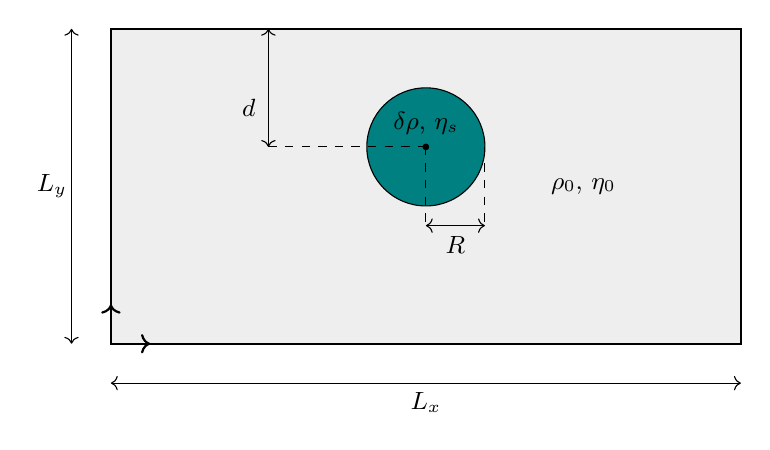
\begin{tikzpicture}
%\draw[step=0.5cm,gray,very thin] (0,0) grid (10,6); %background grid
\draw[fill=gray!63,gray!13](1,1) rectangle (9,5);
\draw[thick] (1,1) -- (9,1) -- (9,5) -- (1,5) -- cycle; %top
\draw[black,fill=teal] (5,3.5)   circle (0.75cm);
\draw[thick,->] (1,1) -- (1.5,1); 
\draw[thick,->] (1,1) -- (1,1.5); 
\draw[black,fill=black] (5,3.5)   circle (1pt);
\draw[thin,<->] (0.5,1) -- (0.5,5); 
\draw[thin,<->] (1,0.5) -- (9,0.5); 
\draw[thin,<->] (3,3.5) -- (3,5); 
\draw[thin,<->] (5,2.5) -- (5.75,2.5); 
\node[] at (5,0.25) {\small $L_x$};
\node[] at (0.25,3) {\small $L_y$};
\node[] at (2.75,4) {\small $d$};
\node[] at (5.375,2.25) {\small $R$};
\draw[dashed,thin] (3,3.5)--(5,3.5);
\draw[dashed,thin] (5,3.5)--(5,2.5);
\draw[dashed,thin] (5.75,3.5)--(5.75,2.5);
\node[] at (7,3) {\small $\rho_0$, $\eta_0$};
\node[] at (5,3.8) {\small $\delta\rho$, $\eta_s$};
\end{tikzpicture}
\end{center}

When the sphere is lighter than its surrounding it goes up and creates a 
divergent flow at the surface. As explained in \textcite{bakp14} an analytical 
solution exists for the horizontal component of the velocity at the surface in 3D. 
Also, the lower density of the sphere (or rather the density difference $\delta\rho$
between the sphere and its surrounding) yields a gravity field 
above the sphere that is lower and for which an analytical solution exists too.

Assuming we have determined what the depth of the sphere is (and assuming that 
it is rigid by taking its viscosity $\eta_s >> \eta_0$), then the two main 
+unknowns are its density difference $\delta \rho$ with regard to the surrounding mantle
and its radius $R$. 

To start with, we can compute analytically the gravity and velocity that a 
$\delta\rho^\dag=-300$ and $R^\dag=50~\si{\km}$ disc generates at the surface of the model,
write a simple inversion code which would operate in the $(R,\delta\rho)$-space 
and automatically looks for the real values of the sphere by computing a gravity misfit $\xi_g$ 
and velocity misfit $\xi_v$ and using these quantities to zero-in on the correct values 
of $\delta \rho$ and $R$.


Three ideas:

- axisymmetric

- full 3D

- try JIT? julia?


%--------------------------------------------------------
\subsection*{gravity forward model - analytical solution}

We consider a circular inclusion at half the 2D domain of 
$1000~\si{\km}$ in $x$- and $500~\si{\km}$ in $y$-direction. 
Because of the evident symmetry of the problem we restrict the 
calculations to the right half of the domain so that now it 
is a square of size $L_x=L_y=500~\si{\km}$ and the sphere is 
at coordinates $(x_c,y_c)=(0,Ly/2)$.

In the case of a disc, the gravity in the $x,y-$plane is given by 
\[
\vec{g}(x,y) = {\cal G} \frac{\pi R^2 \delta\rho}{(x-x_c)^2+(y-y_c)^2} 
\left(
\begin{array}{c}
x-x_c \\
y-y_c
\end{array}
\right)
\]
In the case of a sphere, 
\[
\vec{g}(x,y,z) = {\cal G} \frac{\pi R^2 \delta\rho}{(x-x_c)^2+(y-y_c)^2+(z-z_c)^2} 
\left(
\begin{array}{c}
x-x_c \\
y-y_c \\
z-z_c 
\end{array}
\right)
\]
Gravity is computed by transforming the integral 
\[
\vec{g}(x,y) = \iiint_V {\cal G} \frac{\rho(x',y',z')}{ (x-x')^2+(y-y')^2+(z-z')^2    } dx'dy'dz'
\]
over the domain by a sum of elemental 
integrals which are then computed by means of the same quadrature as the FE matrix. 
Since half the disk is missing, we on-the-fly take the missing half into account by 
mirroring the quadrature points and adding their contribution. 

Because we are only interested in the gravity signal generated by the disc/sphere, 
a boolean array {\tt elt\_in\_sphere} is created and set to true for those elements
for which at least one quadrature point is inside the sphere. This array is then used
to target the contribution of the elements 'inside' the sphere. 



%--------------------------------------------------------
\subsection*{Stokes forward model - analytical solution}

The surface velocity signal of a rising sphere is computed in Appendix~A of \textcite{bakp14} (2014).
It is based on \textcite{bren61} (1961), \textcite{stje26} (1926) and \textcite{pacy05} (2005). See also 
\textcite{burg16} (1916). The solution is only available in 3D with axisymmetric geometry. 
The analytical expression is rather complex and in order to keep simple for now, we
will use a different reference velocity quantity to carry out the inversion. 
In the folder {\tt reference\_code} a modified version of \stone~2 is placed. 
It computes the velocity field for the reference case
at a 150x150 resolution. The root mean square velocity 
$\upnu_{rms}=7.740432578645655e-10~\si{\meter\per\second}$ 
will serve as our reference value to drive the inversion.

\begin{center}
\includegraphics[width=6cm]{python_codes/fieldstone_114/reference_code/vel}
\includegraphics[width=6cm]{python_codes/fieldstone_114/reference_code/eta}\\
{\captionfont Sphere radius is $R=50~\si{\km}$, $\rho_m=3000$, $\delta\rho=-300$, $\eta^\star=10^3$.}
\end{center}

%--------------------------------------------------------
\subsection*{The code}

In order to produce a reasonably fast Stokes solver the code relies on 
the $Q_1\times P_0$ element with a penalty approach (see for example \stone~01).
The Cartesian domain is overlain with a mesh counting $nel_x\times nel_y=nel$
elements which are all square, so that the Jacobian of the transformation
between global and local coordinates is diagonal. Its value has been 
hard-wired in the code so as to save time. 
The entire Stokes solver + gravity calculator is inserted into a single function
{\tt compute\_misfits} in the {\pythonfile forward.py} file.

Note that depending on the mesh resolution a call to the function will take betweem 1s 
(50x50) 2.5s (64x64), and 8s (100x100). 

%--------------------------------------------------------
\subsection*{Inversion}

The first inversion code {\pythonfile driver1.py} is very simple. The user defines the bounds of the 
parameter space, i.e. $\delta\rho_{min}$, $\delta\rho_{max}$, $R_{min}$ and $R_{max}$.
Then a regular grid composed of $n_{\delta\rho} \times n_{R}$ is used to compute 
both misfits $\xi_g$ and $\xi_v$ at each node of the grid and these are 
exported in a vtu file. No refinement or clever search takes place. 

\begin{center}
\includegraphics[width=5.7cm]{python_codes/fieldstone_114/results/min}
\includegraphics[width=5.7cm]{python_codes/fieldstone_114/results/mg}
\includegraphics[width=5.7cm]{python_codes/fieldstone_114/results/mv}\\
{\captionfont horizontal axis is radius $R$, vertical axis is $\delta\rho$. 60x60 points. about 2.5h.
Left: location of the true minimum, i.e. the reference model; Middle: gravity misfit; Right: vrms misfit.} 
\end{center}




 %%%%%%%%%%%%%%%%%%%%%%%%%%%%%%%%%%%%%%%%%%%%%%%%%%%%%%%%%%

\chapter{$Q_1\times P_0$-stab element for isoviscous flow \label{f115}} %%%%%%%%%%%%%%%%%%%%%%%%%%% 115
\includegraphics[height=1.5cm]{images/pictograms/benchmark}

\begin{flushright} {\tiny {\color{gray} python\_codes/fieldstone\_115/text.tex}} \end{flushright}

\lstinputlisting[language=bash,basicstyle=\small]{python_codes/fieldstone_115/keywords.ascii}

\begin{center}
\fbox{\textbf{\huge \color{teal} P}}
Codes at \url{https://github.com/cedrict/fieldstone/tree/master/python_codes/fieldstone_115}
\end{center}

\par\noindent\rule{\textwidth}{0.4pt}

%%%%%%%%%%%%%%%%%%%%%%%%%%%%%%%%%%%%%%%%%%%%%%%%%%%%%%%%%%%%%%%%%%%%%%%%%%%%%%%%%%%%%%%%%%%%%%



When it comes to the stabilisation of the $Q_1\times P_0$ elements, 
we have seen in Section~\ref{ss:pairq1p0stab} that mulitple types co-exist
and that a tuning parameter $\epsilon$ plays a role. 
Despite the published literature on the topic, the following questions remain:

- how to deal with vicosity contrasts ? 

- which stab is best for real life geodynamics ? 

- how to deal with not square mesh ?

- how to choose the $\epsilon$ value ?

- look at buoyancy driven flows. lith pressure!

- I have implemented penalty, global, local and macro-element. what about the other methods, eg bodg06 ?

- concretely how would PCG converge?

The code is based on \stone 14.

Velocity divergence is measured at the center of the element.

note that in case of penalty, $\epsilon$ should be $\sim 10^6$ larger than viscosity.

%====================================================================================
\subsection*{Donea \& Huerta manufactured solution}


\begin{center}
\includegraphics[width=5cm]{python_codes/fieldstone_115/results/dh/nostab/matrix}
\includegraphics[width=5cm]{python_codes/fieldstone_115/results/dh/penalty/matrix}
\includegraphics[width=5cm]{python_codes/fieldstone_115/results/dh/global/matrix}\\
\includegraphics[width=5cm]{python_codes/fieldstone_115/results/dh/local/matrix}
\includegraphics[width=5cm]{python_codes/fieldstone_115/results/dh/macro/matrix}\\
{\captionfont 32x32. From left to right: parsity pattern of the FEM matric for 
no stabilisation, penalty, global, local, macro-elt.}
\end{center}

We find that all three stabilisation $\C$ matrices are enough to suppress the chequerboard mode:
\begin{center}
\includegraphics[width=3.4cm]{python_codes/fieldstone_115/results/dh/p0}
\includegraphics[width=3.4cm]{python_codes/fieldstone_115/results/dh/p1}
\includegraphics[width=3.4cm]{python_codes/fieldstone_115/results/dh/p2}
\includegraphics[width=3.4cm]{python_codes/fieldstone_115/results/dh/p3}
\includegraphics[width=3.4cm]{python_codes/fieldstone_115/results/dh/p4}\\
{\captionfont resolution $32\times 32$. From left to right: no stabilisation, penalty, 
global, local, macro-elt. $\epsilon=10^{-1}$}
\end{center}

We can now explore the influence of the stabilisation parameter $\epsilon$. Obviously, 
if too low it won't have any effect as the $\C$ matrix then tends to zero. If too high,
then we expect it to perturb the solution too much. 
The pressure field is shown in the following figure for various values of $\epsilon$, 


\begin{center}
\includegraphics[width=3.4cm]{python_codes/fieldstone_115/results/dh/pressure_nostab.pdf}
\includegraphics[width=3.4cm]{python_codes/fieldstone_115/results/dh/pressure_penalty.pdf}
\includegraphics[width=3.4cm]{python_codes/fieldstone_115/results/dh/pressure_global.pdf}
\includegraphics[width=3.4cm]{python_codes/fieldstone_115/results/dh/pressure_local.pdf}
\includegraphics[width=3.4cm]{python_codes/fieldstone_115/results/dh/pressure_macro.pdf}\\
\includegraphics[width=3.4cm]{python_codes/fieldstone_115/results/dh/pressure_nostab_error.pdf}
\includegraphics[width=3.4cm]{python_codes/fieldstone_115/results/dh/pressure_penalty_error.pdf}
\includegraphics[width=3.4cm]{python_codes/fieldstone_115/results/dh/pressure_global_error.pdf}
\includegraphics[width=3.4cm]{python_codes/fieldstone_115/results/dh/pressure_local_error.pdf}
\includegraphics[width=3.4cm]{python_codes/fieldstone_115/results/dh/pressure_macro_error.pdf}\\
{\captionfont 32x32. pressure profile.} 
\end{center}

Let us now turn to the velocity and pressure error convergence rates: 
\begin{center}
\includegraphics[width=4.21cm]{python_codes/fieldstone_115/results/dh/errorsV_penalty.pdf}
\includegraphics[width=4.21cm]{python_codes/fieldstone_115/results/dh/errorsV_global.pdf}
\includegraphics[width=4.21cm]{python_codes/fieldstone_115/results/dh/errorsV_local.pdf}
\includegraphics[width=4.21cm]{python_codes/fieldstone_115/results/dh/errorsV_macro.pdf}\\
\includegraphics[width=4.21cm]{python_codes/fieldstone_115/results/dh/errorsP_penalty.pdf}
\includegraphics[width=4.21cm]{python_codes/fieldstone_115/results/dh/errorsP_global.pdf}
\includegraphics[width=4.21cm]{python_codes/fieldstone_115/results/dh/errorsP_local.pdf}
\includegraphics[width=4.21cm]{python_codes/fieldstone_115/results/dh/errorsP_macro.pdf}\\
\includegraphics[width=4.21cm]{python_codes/fieldstone_115/results/dh/divv_penalty.pdf}
\includegraphics[width=4.21cm]{python_codes/fieldstone_115/results/dh/divv_global.pdf}
\includegraphics[width=4.21cm]{python_codes/fieldstone_115/results/dh/divv_local.pdf}
\includegraphics[width=4.21cm]{python_codes/fieldstone_115/results/dh/divv_macro.pdf}\\
{\captionfont Velocity and pressure errors as a function of the element size for meshes 6x6 to 144x144}
\end{center}
We find that the error convergence rate for velocity is always quadratic as expected, 
while the error convergence for pressure becomes monotonous and linear as expected too.

It also appears that the macro-element technique is the least sensitive to the value of $\epsilon$, 
although it is rather surprising that even very low values of $\epsilon$ manage to stabilise the 
system so well. could it be because this benchmark is very smooth? 
\begin{center}
\includegraphics[width=5.7cm]{python_codes/fieldstone_115/results/dh/errorsP_32_eps}
\includegraphics[width=5.7cm]{python_codes/fieldstone_115/results/dh/errorsP_64_eps}
\includegraphics[width=5.7cm]{python_codes/fieldstone_115/results/dh/errorsP_96_eps}\\
{\captionfont Influence of $\epsilon$ parameter on pressure error.}
\end{center}

{\bf Conclusion}: macro-element technique yields best results: lower velocity divergence, 
least sensitive to $\epsilon$ value, block matrix,

I should monitor the condition number of the matrix...

\newpage
%====================================================================================
\subsection*{The aquarium}

The domain is still a unit square. Boundary conditions are no slip on all sides. 
Density and viscosity are set to 1. Gravity is vertical with $\vec{g}=-\vec{e}_y$.
The analytical velocity is obviously $\vec\upnu=\vec{0}$ and the analytical pressure
is $p(x,y)=0.5-y$ (which fulfils $\int_\Omega p dV=0$).

Because the analytical velocity field is a constant, it can be represented exactly 
by bi-linear functions so we expect the velocity error to be at machine precision
independently of the resolution. However, because of the presence of the stabilisation
term, we find in the penalty case that it is proportional to $\epsilon$ and 
in the global and local cases that it converges quadratically.

The analytical pressure field, on the other hand is a linear polynomial which cannot 
be represented exactly by a set of discontinuous $C^0$ functions. We then expect and 
indeed recover a linear convergence.


\begin{center}
\includegraphics[width=4.21cm]{python_codes/fieldstone_115/results/aquarium/errorsV_penalty.pdf}
\includegraphics[width=4.21cm]{python_codes/fieldstone_115/results/aquarium/errorsV_global.pdf}
\includegraphics[width=4.21cm]{python_codes/fieldstone_115/results/aquarium/errorsV_local.pdf}
\includegraphics[width=4.21cm]{python_codes/fieldstone_115/results/aquarium/errorsV_macro.pdf}\\
\includegraphics[width=4.21cm]{python_codes/fieldstone_115/results/aquarium/errorsP_penalty.pdf}
\includegraphics[width=4.21cm]{python_codes/fieldstone_115/results/aquarium/errorsP_global.pdf}
\includegraphics[width=4.21cm]{python_codes/fieldstone_115/results/aquarium/errorsP_local.pdf}
\includegraphics[width=4.21cm]{python_codes/fieldstone_115/results/aquarium/errorsP_macro.pdf}\\
\includegraphics[width=4.21cm]{python_codes/fieldstone_115/results/aquarium/divv_penalty.pdf}
\includegraphics[width=4.21cm]{python_codes/fieldstone_115/results/aquarium/divv_global.pdf}
\includegraphics[width=4.21cm]{python_codes/fieldstone_115/results/aquarium/divv_local.pdf}
\includegraphics[width=4.21cm]{python_codes/fieldstone_115/results/aquarium/divv_macro.pdf}\\
{\captionfont Velocity and pressure errors as a function of the element size for meshes 6x6 to 144x144}
\end{center}


\begin{center}
\includegraphics[width=5.7cm]{python_codes/fieldstone_115/results/aquarium/errorsP_32_eps}
\includegraphics[width=5.7cm]{python_codes/fieldstone_115/results/aquarium/errorsP_64_eps}
\includegraphics[width=5.7cm]{python_codes/fieldstone_115/results/aquarium/errorsP_96_eps}\\
{\captionfont Influence of $\epsilon$ parameter on pressure error.}
\end{center}


\newpage
%====================================================================================
\subsection*{Lid driven cavity}

This is not a benchmark but a simple setup which is not very physical. The most right and left
points of the lid have zero velocity ('non-leaky cavity').

We find that in the absence of stabilisation the pressure chequerboard mode is 
very strong:
\begin{center}
\includegraphics[width=5.7cm]{python_codes/fieldstone_115/results/ldc/nostab/vel}
\includegraphics[width=5.7cm]{python_codes/fieldstone_115/results/ldc/nostab/p}
\includegraphics[width=5.7cm]{python_codes/fieldstone_115/results/ldc/psurf_nostab.pdf}\\
{\captionfont No stabilisation: velocity and pressure at 32x32. Right: 
pressure at the top at various resolutions.}
\end{center}

\begin{center}
\includegraphics[width=5.7cm]{python_codes/fieldstone_115/results/ldc/psurf_penalty.pdf}
\includegraphics[width=5.7cm]{python_codes/fieldstone_115/results/ldc/psurf_global.pdf}\\
\includegraphics[width=5.7cm]{python_codes/fieldstone_115/results/ldc/psurf_local.pdf}
\includegraphics[width=5.7cm]{python_codes/fieldstone_115/results/ldc/psurf_macro.pdf}\\
{\captionfont Pressure at the top at $128\times 128$ resolution.}
\end{center}

\begin{center}
\includegraphics[width=4cm]{python_codes/fieldstone_115/results/ldc/vrms_penalty.pdf}
\includegraphics[width=4cm]{python_codes/fieldstone_115/results/ldc/vrms_global.pdf}
\includegraphics[width=4cm]{python_codes/fieldstone_115/results/ldc/vrms_local.pdf}
\includegraphics[width=4cm]{python_codes/fieldstone_115/results/ldc/vrms_macro.pdf}\\
\includegraphics[width=4cm]{python_codes/fieldstone_115/results/ldc/prms_penalty.pdf}
\includegraphics[width=4cm]{python_codes/fieldstone_115/results/ldc/prms_global.pdf}
\includegraphics[width=4cm]{python_codes/fieldstone_115/results/ldc/prms_local.pdf}
\includegraphics[width=4cm]{python_codes/fieldstone_115/results/ldc/prms_macro.pdf}\\
\includegraphics[width=4cm]{python_codes/fieldstone_115/results/ldc/divv_penalty.pdf}
\includegraphics[width=4cm]{python_codes/fieldstone_115/results/ldc/divv_global.pdf}
\includegraphics[width=4cm]{python_codes/fieldstone_115/results/ldc/divv_local.pdf}
\includegraphics[width=4cm]{python_codes/fieldstone_115/results/ldc/divv_macro.pdf}\\
{\captionfont Left to right: penalty, global, local, macro-element}
\end{center}

\newpage
%==============================================================================
\subsection*{Manufactured solution of \textcite{buha06}}

See section~\ref{ss:mms_buha06}.
The velocity and pressure fields are given in the unit square by
\begin{eqnarray}
u(x,y) &=& 20xy^3 \nn\\
v(x,y) &=& 5x^4-5y^4 \nn\\
p(x,y) &=& 60x^2y -20y^3 -5
\end{eqnarray}


\begin{center}
\includegraphics[width=4cm]{python_codes/fieldstone_115/results/buha06/errorsV_penalty.pdf}
\includegraphics[width=4cm]{python_codes/fieldstone_115/results/buha06/errorsV_global.pdf}
\includegraphics[width=4cm]{python_codes/fieldstone_115/results/buha06/errorsV_local.pdf}
\includegraphics[width=4cm]{python_codes/fieldstone_115/results/buha06/errorsV_macro.pdf}\\
\includegraphics[width=4cm]{python_codes/fieldstone_115/results/buha06/errorsP_penalty.pdf}
\includegraphics[width=4cm]{python_codes/fieldstone_115/results/buha06/errorsP_global.pdf}
\includegraphics[width=4cm]{python_codes/fieldstone_115/results/buha06/errorsP_local.pdf}
\includegraphics[width=4cm]{python_codes/fieldstone_115/results/buha06/errorsP_macro.pdf}\\
\includegraphics[width=4cm]{python_codes/fieldstone_115/results/buha06/divv_penalty.pdf}
\includegraphics[width=4cm]{python_codes/fieldstone_115/results/buha06/divv_global.pdf}
\includegraphics[width=4cm]{python_codes/fieldstone_115/results/buha06/divv_local.pdf}
\includegraphics[width=4cm]{python_codes/fieldstone_115/results/buha06/divv_macro.pdf}\\
{\captionfont Velocity and pressure errors as a function of the element size for meshes 6x6 to 144x144.
Left to right: penalty, global, local, macro-element}
\end{center}



\begin{center}
\includegraphics[width=3.2cm]{python_codes/fieldstone_115/results/buha06/p0}
\includegraphics[width=3.2cm]{python_codes/fieldstone_115/results/buha06/p1}
\includegraphics[width=3.2cm]{python_codes/fieldstone_115/results/buha06/p2}
\includegraphics[width=3.2cm]{python_codes/fieldstone_115/results/buha06/p3}
\includegraphics[width=3.2cm]{python_codes/fieldstone_115/results/buha06/p4}\\
\includegraphics[width=3.2cm]{python_codes/fieldstone_115/results/buha06/divv0}
\includegraphics[width=3.2cm]{python_codes/fieldstone_115/results/buha06/divv1}
\includegraphics[width=3.2cm]{python_codes/fieldstone_115/results/buha06/divv2}
\includegraphics[width=3.2cm]{python_codes/fieldstone_115/results/buha06/divv3}
\includegraphics[width=3.2cm]{python_codes/fieldstone_115/results/buha06/divv4}\\
{\captionfont 64x64, epsi=0.1. Left to right: no stab, penalty, global, local, macro-elt.
Top row is pressure, bottom row is elemental velocity divergence.}
\end{center}



\begin{center}
\includegraphics[width=5.7cm]{python_codes/fieldstone_115/results/buha06/errorsP_32_eps}
\includegraphics[width=5.7cm]{python_codes/fieldstone_115/results/buha06/errorsP_64_eps}
\includegraphics[width=5.7cm]{python_codes/fieldstone_115/results/buha06/errorsP_96_eps}\\
{\captionfont Influence of $\epsilon$ parameter on pressure error for global, local, macro-elt}
\end{center}
 %%%%%%%%%%%%%%%%%%%%%%%%%%%%%%%%%%%%%%%%%%%%%%%%%%%%%%%%%% 

\chapter{$Q_1\times P_0$-stab element with viscosity contrasts\label{f116}} %%%%%%%%%%%%%%%%%%%%%%% 116
\begin{flushright} {\tiny {\color{gray} python\_codes/fieldstone\_116/text.tex}} \end{flushright}

\lstinputlisting[language=bash,basicstyle=\small]{python_codes/fieldstone_116/keywords.ascii}

\begin{center}
\fbox{\textbf{\huge \color{teal} P}}
Codes at \url{https://github.com/cedrict/fieldstone/tree/master/python_codes/fieldstone_116}
\end{center}

\par\noindent\rule{\textwidth}{0.4pt}

%%%%%%%%%%%%%%%%%%%%%%%%%%%%%%%%%%%%%%%%%%%%%%%%%%%%%%%%%%%%%%%%%%%%%%%%%%%%%%%%%%%%%%%%%%%%%%

As we have seen in Section~\ref{XXXX} the formulation of the $\C$ matrix is substantially 
less straightforward when viscosity variations/contrasts are present in the domain. 

This stone builds on the previous \stone~115 and explores the various approaches for 
mutiple typical manufactured solutions (SolCx, SolKz, SolVi, ...).





In the case of the macro element stabilisation, an effective viscosity is computed based on the 
elemental viscosity inside the 4 elements. 


%======================================================
\subsection*{SolKz}

we start with SolKz, which showcases 6 orders of magnitude viscosity variation in the 
domain albeit in a very smooth way:
\[
\eta(x,y)=\exp (2 B y) \qquad \text{with} \qquad B=13.8155
\]




 %%%%%%%%%%%%%%%%%%%%%%%%%%%%%%%%%%%%%%%%%%%%%%%%%%%%%%%%%%

\chapter{circular inclusion with bespoke mesh \label{f117}} %%%%%%%%%%%%%%%%%%%%%%%%%%%%%%%%%%%%%%% 117
\begin{flushright} {\tiny {\color{gray} python\_codes/fieldstone\_117/text.tex}} \end{flushright}

\lstinputlisting[language=bash,basicstyle=\small]{python_codes/fieldstone_117/keywords.ascii}

\begin{center}

\fbox{\textbf{\huge \color{teal} P}}
Codes at \url{https://github.com/cedrict/fieldstone/tree/master/python_codes/fieldstone_01}
\end{center}

\par\noindent\rule{\textwidth}{0.4pt}

{\sl This fieldstone was developed in collaboration with Lukas van de Wiel}. \index{contributors}{L. van de Wiel}

\par\noindent\rule{\textwidth}{0.4pt}
%%%%%%%%%%%%%%%%%%%%%%%%%%%%%%%%%%%%%%%%%%%%%%%%%%%%%%%%%%%%%%%%%%%%%%%%%%%%%%%%%%%%%%%%%%%%%%

This is work in progress. There is still much to do. The idea here is to compare the 
accuracy of quads on a specific benchmark (SolVi) as obtained on a bespoke mesh.

%-------------------------------
\subsection*{The mesh}

The mesh(es) used in this \stone are obtained by means of the quilt mesher program written by Lukas. 

INSERT HERE MANUAL


In order to generate the meshes that the \stone needs, we need to modify two files:
\begin{itemize}
\item {\tt quilt.f}: elementType = Q0, Q1, Q2, Q3, or Q4
\item {\tt examples.f}: in subroutine meshThirteenPatches: nElemsBase=10
\end{itemize}

WARNING! As of now the edges of the elements are straight, so that the mid-egde nodes do not 
follow the curvature of the inclusion.

%-------------------------------
\subsection*{The benchmarks}

I have implemented five finite element pairs: $Q_1\times P_0$, $Q_2\times Q_1$, $Q_2 \times P_{-1}$
(both mapped and unmapped flavours), $Q_3\times Q_2$, $Q_4\times Q_3$. 
Note that unfortunately the vtu format does not allow the representation of $Q_3$ or $Q_4$ fields. 
The basis functions for all these elements are to be found in Section~\ref{sec:shpfct2d}.

Two benchmarks are implemented in the code: Donea \& Huerta (see Section~\ref{mms1}) and 
SolVi (see Section~\ref{ss:solvi}).
The first one is a manufactured solution which has a vertical and horizontal symmetry. 
As such the tailored mesh is of no use here. The second is of course why the mesher 
was developed in the first place: the viscosity contrast between 
inclusion and matrix aligns exactly with the mesh:

\begin{center}
\includegraphics[width=5cm]{python_codes/fieldstone_117/images/mesh04}
\includegraphics[width=5cm]{python_codes/fieldstone_117/images/mesh10}
\includegraphics[width=5cm]{python_codes/fieldstone_117/images/mesh20}\\
{\captionfont Mesh generated with nElemsBase=4,10,20.}
\end{center}

\begin{center}
\begin{tabular}{ll}
\hline
{\tt element} & FE pair \\
\hline
\hline
1& $Q_1 \times P_0$ \\
2& $Q_2 \times Q_1$ \\
3& $Q_3 \times Q_2$ \\
4& $Q_4 \times Q_3$ \\
5& $Q_2 \times P_{-1}$ (mapped)\\
6& $Q_2 \times P_{-1}$ (unmapped)\\
\hline
\end{tabular}
\end{center}

manifold for viscosity interface?

do Q2(8)Q1


\begin{center}
\includegraphics[width=7.5cm]{python_codes/fieldstone_117/results/errorsV}
\includegraphics[width=7.5cm]{python_codes/fieldstone_117/results/errorsP}\\
{\captionfont SolVi benchmark: Velocity and pressure errors as a function of the largest element size in the mesh.}
\end{center}

include figure of p at bottom
 %%%%%%%%%%%%%%%%%%%%%%%%%%%%%%%%%%%%%%%%%%%%%%%%%%%%%%%%%%

\chapter{subduction initiation in the 80's ($Q_2\times Q_1$) \label{f118}} %%%%%%%%%%%%%%%%%%%%%%%% 118
\begin{flushright} {\tiny {\color{gray} python\_codes/fieldstone\_118/text.tex}} \end{flushright}

\lstinputlisting[language=bash,basicstyle=\small]{python_codes/fieldstone_118/keywords.ascii}

\begin{center}
\fbox{\textbf{\huge \color{teal} P}}
Files at \url{https://github.com/cedrict/fieldstone/tree/master/python_codes/fieldstone_118}
\end{center}

\par\noindent\rule{\textwidth}{0.4pt}

%%%%%%%%%%%%%%%%%%%%%%%%%%%%%%%%%%%%%%%%%%%%%%%%%%%%%%%%%%%%%%%%%%%%%%%%%%%%%%%%%%%%%%%%%%%%%%

The setup is taken from \textcite{mato83} (1983) and \textcite{futo85} (1985).
The true motivation here is to replicate the 1985 study 
and have a reason to focus on the following most improbable figure in a peer reviewed
article in geosciences:

\begin{center}
\includegraphics[width=12cm]{./images/interesting/futo85}\\
{\captionfont Taken from \textcite{futo85} (1985).}
\end{center}

In the original paper (1983) the authors solve the incompressible isothermal Stokes equations
with a stream function approach. The resulting equation is solved by means of the
Finite Difference method and the Marker and Cell (MAC) method \cite{hawe65}.

The domain is a 2D Cartesian box of size $L_x \times L_y=(400,180)~\si{\km}$. 
There are three fluids in the domain: 
water ($\rho_w=1030~\si{\kg\per\cubic\meter}$, $\eta_w=10^{-3}~\si{\pascal\second}$), 
lithosphere ($\rho_l=3300~\si{\kg\per\cubic\meter}$, $\eta_l$) and 
asthenosphere ($\rho_a=3200~\si{\kg\per\cubic\meter}$, $\eta_a$).
Boundary conditions are free-slip on all sides of the domain.
Unfortunately the authors do not specify the mesh resolution that was used. 

Six cases are considered\footnote{Note that in the paper all viscosities 
are expressed in Poise, with 1~Poise=0.1~\si{\pascal\second}}:
\begin{center}
\begin{tabular}{lccc}
Case & $\eta_l$ (\si{\pascal\second}) & $\eta_a$  (\si{\pascal\second}) & domain size (\si{\km})\\
\hline
1 & $10^{22}$ & $10^{21}$ & $400\times 180$\\
2 & $10^{22}$ & $10^{20}$ & $400\times 180$\\
3 & $10^{22}$ & $10^{19}$ & $400\times 180$\\
4 & $10^{23}$ & $10^{21}$ & $400\times 180$\\
\hline
5 & $10^{22}$ & $10^{20}$ & $800\times 140$\\
6 & $10^{22}$ & $10^{19}$ & $800\times 140$\\
\hline
\end{tabular}
\end{center}

\begin{center}
\includegraphics[width=7cm]{python_codes/fieldstone_118/images/mato83}\\
{\captionfont Taken from \textcite{mato83}. Dw=10km, Dl=50km, dw=8km, 
dl=10km, $L_0=3L_x/4$. Blue numbers indicate the numbering of each compositional field.}
\end{center}

Interestingly the authors state: ``The materials are initially placed so that 
uniform hydrostatic pressure holds at the bottom of the calculation area''. 
On the left side, the pressure at the bottom is given by 
\[
p_b=(10\cdot 1030+50\cdot 3300+80\cdot3200)g_y = 431,300g_y
\]
while on the right side it is
\[
p_b=(8\cdot 1030+10\cdot 3300+122 \cdot3200)g_y = 431,640g_y
\]
which means that indeed the system is in isostatic equilibrium at the beginning of the 
simulation. 

The authors use a CFL condition to determine the time step $\delta t$ and use an arithmetic 
averaging scheme for both density and viscosity.

%%%%%%%%%%%%%%%%%%%%%%%%%%%%%%%%%%%%%%%%%%%%%%%%%%%%%%%%%%%%%%%%%%%%%%%
\subsection*{Using Aspect}

I am using here \aspect and the input files are included in the folder (in 
what follows I have used the one based on compositional fields but there
is also a second prm file based on particles). It is straightforward 
since the flow is isothermal and incompressible and the domain a Cartesian box with 
free slip boundary conditions. A pressure normalisation is then necessary to remove 
the pressure nullspace and the pressure is then set to zero on average on the top boundary. 
A CFL condition is used with $C=0.25$ and the models 
are run 50~\si{\mega\year}. 
Two repetitions are used in the horizontal directions so that elements are almost square.
The mesh counts $128\times 64=8192$ cells, i.e. a resolution of about 3~\si{\km} which is barely enough to 
accurately follow the thin lithosphere.


%%%%%%%%%%%%%%%%%%%%%%%%%%%%%%%%%%%%%%%%%%%%%%%%%%%%%%%%%%%%%%%%%%%%%%%
\subsection*{This stone (instantaneous)}

I have also written a $Q_2\times Q_1$ code which is able to 
compute the solution of the problem at $t=0$ (it stems from \stone 40). 
It does not feature any algorithm to advect interfaces or fluids and
it is also quite naive and relies on full matrices for the 
blocks of the Stokes matrix. Nevertheless, it allows to compute the solution 
on a $80\times 90$ mesh, i.e. a $5\times 2~\si{\km}$ resolution with 
all fluid boundaries alligned with mesh boundaries:

\begin{center}
\includegraphics[width=5.6cm]{python_codes/fieldstone_118/results/case1/stone/vel}
\includegraphics[width=5.6cm]{python_codes/fieldstone_118/results/case1/stone/u}
\includegraphics[width=5.6cm]{python_codes/fieldstone_118/results/case1/stone/v}\\
\includegraphics[width=5.6cm]{python_codes/fieldstone_118/results/case1/stone/sr}
\includegraphics[width=5.6cm]{python_codes/fieldstone_118/results/case1/stone/eta}
\includegraphics[width=5.6cm]{python_codes/fieldstone_118/results/case1/stone/rho}\\
{\captionfont Results obtained with this \stone, resolution  $80\times 90$ for Case 1.}
\end{center}

\newpage

%%%%%%%%%%%%%%%%%%%%%%%%%%%%%%%%%%%%%%%%%%%%%%%%%%%%%%%%%%%%%%%%%%%%%%%
\subsection*{Results - Case 1}

Results obtained with \aspect agree nicely with those of the paper
although the water layer and the thin lithosphere is much more 
deformed in their case. The run took approx. 6500~s to complete on a single core.

\begin{center}
\includegraphics[width=3.25cm]{python_codes/fieldstone_118/images/case1/a}
\includegraphics[width=3.25cm]{python_codes/fieldstone_118/images/case1/b}
\includegraphics[width=3.25cm]{python_codes/fieldstone_118/images/case1/c}
\includegraphics[width=3.25cm]{python_codes/fieldstone_118/images/case1/d}
\includegraphics[width=3.25cm]{python_codes/fieldstone_118/images/case1/e}\\
\includegraphics[width=3.25cm]{python_codes/fieldstone_118/results/case1/a}
\includegraphics[width=3.25cm]{python_codes/fieldstone_118/results/case1/b}
\includegraphics[width=3.25cm]{python_codes/fieldstone_118/results/case1/c}
\includegraphics[width=3.25cm]{python_codes/fieldstone_118/results/case1/d}
\includegraphics[width=3.25cm]{python_codes/fieldstone_118/results/case1/e}\\
{\captionfont System at times 0, 10, 20, 30 and 50~Myr.}
\end{center}


\begin{center}
\includegraphics[width=4cm]{python_codes/fieldstone_118/results/case1/vel}
\includegraphics[width=4cm]{python_codes/fieldstone_118/results/case1/rho}
\includegraphics[width=4cm]{python_codes/fieldstone_118/results/case1/eta}
\includegraphics[width=4cm]{python_codes/fieldstone_118/results/case1/sr}\\
{\captionfont Various fields at $t=50$ Myr.}
\end{center}

%%%%%%%%%%%%%%%%%%%%%%%%%%%%%%%%%%%%%%%%%%%%%%%%%%%%%%%%%%%%%%%%%%%%%%%
\subsection*{Results - Case 1* }

This case is not in the original publication. It consists of Case 1 run with a 
50\% longer domain, all other things equal (with $L_0=2L_x/3$). We find that the domain size does not
play a large role in the model evolution at all: 

\begin{center}
\includegraphics[width=9cm]{python_codes/fieldstone_118/results/case1b/isos}\\
{\captionfont Compositional fields isolines at $t=50$ Myr. Black lines correspond
to 600x180 domain while blue lines correspond to 400x180km domain.}
\end{center}

%%%%%%%%%%%%%%%%%%%%%%%%%%%%%%%%%%%%%%%%%%%%%%%%%%%%%%%%%%%%%%%%%%%%%%%
\subsection*{Results - Case 2}

\begin{center}
\includegraphics[width=3.25cm]{python_codes/fieldstone_118/images/case2/a}
\includegraphics[width=3.25cm]{python_codes/fieldstone_118/images/case2/b}
\includegraphics[width=3.25cm]{python_codes/fieldstone_118/images/case2/c}\\
\includegraphics[width=3.25cm]{python_codes/fieldstone_118/results/case2/a}
\includegraphics[width=3.25cm]{python_codes/fieldstone_118/results/case2/b}
\includegraphics[width=3.25cm]{python_codes/fieldstone_118/results/case2/c}\\
{\captionfont System at times 9.6, 16.6 and 25.1~\si{\mega\year}.}
\end{center}

\begin{center}
\includegraphics[width=4cm]{python_codes/fieldstone_118/results/case2/vel}
\includegraphics[width=4cm]{python_codes/fieldstone_118/results/case2/rho}
\includegraphics[width=4cm]{python_codes/fieldstone_118/results/case2/eta}
\includegraphics[width=4cm]{python_codes/fieldstone_118/results/case2/sr}\\
{\captionfont Various fields at $t=25.1~\si{\mega\year}$.}
\end{center}



TODO: run stone 67 with pic!

 %%%%%%%%%%%%%%%%%%%%%%%%%%%%%%%%%%%%%%%%%%%%%%%%%%%%%%%%%%

\chapter{on computing the lithostatic pressure in geodynamical models \label{f119}} %%%%%%%%%%%%%%% 119
\begin{flushright} {\tiny {\color{gray} python\_codes/fieldstone\_119/text.tex}} \end{flushright}

\lstinputlisting[language=bash,basicstyle=\small]{python_codes/fieldstone_119/keywords.ascii}

\begin{center}

\fbox{\textbf{\huge \color{teal} P}}
Codes at \url{https://github.com/cedrict/fieldstone/tree/master/python_codes/fieldstone_01}
\end{center}

\par\noindent\rule{\textwidth}{0.4pt}

{\sl This stone was developed with input from Anthony Jourdon, Wolfgang Bangerth and Bob Myhill}. 
%\index{contributors}{J. Mos}

\par\noindent\rule{\textwidth}{0.4pt}
%%%%%%%%%%%%%%%%%%%%%%%%%%%%%%%%%%%%%%%%%%%%%%%%%%%%%%%%%%%%%%%%%%%%%%%%%%%%%%%%%%%%%%%%%%%%%%

\subsection*{About lithostatic pressure}

Let us look in section 2.2 of \textcite{tusc}:
``The normal force per unit area on horizontal planes increases linearly with
depth. The normal stress due to the weight of the overlying rock or over-
burden is known as the lithostatic stress or pressure.''

Also, on wikipedia\footnote{\url{https://en.wikipedia.org/wiki/Overburden_pressure}}:
``
Pressure is force magnitude applied over an area. Overburden pressure is a geology term that denotes the pressure caused by 
the weight of the overlying layers of material at a specific depth under the earth's surface.
Overburden pressure is also called lithostatic pressure, or vertical stress.
In a stratigraphic layer that is in hydrostatic equilibrium; the overburden pressure at a depth $z$, assuming the magnitude 
of the gravity acceleration is approximately constant, is given by: 
\[
P(z)=P_0 + g \int_0^z \rho(z) dz
\]
where $z$ is the depth in meters, $P(z)$ is the overburden pressure at depth $d$,
$P_0$ is the pressure at the surface, $\rho(z)$ is the density of the material above the depth $z$,
$g$ is the gravity acceleration in \si{\meter\per\square\second}.

In deep-earth geophysics/geodynamics, gravitational acceleration varies significantly over depth and $g$
should not be assumed to be constant, and should be inside the integral. ''

Finally, in Gerya's book:
``In geosciences, pressure is often considered as corresponding to the hydrostatic (litho-
static) condition everywhere and it is computed as a function of depth $y$ and vertical density
profile $\rho(y)$
\[
P(y)=P_0 + g \int_0^y \rho(y) dy
\]
where $P_0=0.1$~MPa is pressure on the Earth’s surface and $g$ is the gravitational
acceleration.''

On the AAPG wiki page\footnote{\url{https://wiki.aapg.org/Geostatic_and_lithostatic_pressure}}:
``The geostatic pressure at a given depth is the vertical pressure due to the weight of a column of 
rock and the fluids contained in the rock above that depth. Lithostatic pressure is the vertical 
pressure due to the weight of the rock only. ''

In conclusion there seems to be a widely accepted definition as to what lithostatic pressure is.
At a given location it is solely given as a function of the column of material 
above it. Since $\rho>0$ and $g>0$ too, the (absolute value of) the lithostatic pressure
can only increase with depth.

%--------------------------------------------------------
\subsection*{The numerical approach of Jourdon \& May (2022)}

What follows is based on \textcite{joma22} (2022) in which the authors present an
``efficient parallel method to compute lithostatic pressure in thermo-mechanical geodynamic models''.

We then start from 
\begin{equation}
-\vec\nabla p + \rho \vec{g} = \vec{0}
\label{eq:gradpstrong}
\end{equation}
and we take the divergence of this expression:
\[
\vec\nabla \cdot \vec\nabla p = \vec\nabla \cdot \rho \vec{g} 
\]
We multiply by a test function $q$ and integrate over the domain:
\[
\int_\Omega q \vec\nabla \cdot \vec\nabla p \;dV
=
\int_\Omega q \vec\nabla \cdot \rho \vec{g} \;dV
\]
We integrate by parts both LHS and RHS :
\[
-\int_\Omega \vec\nabla q \cdot  \vec\nabla p \;dV + \int_\Gamma q \vec\nabla p \cdot \vec{n} \;dS
=
-\int_\Omega  \vec\nabla q \cdot  \rho \vec{g} \;dV + \int_\Gamma q \rho \vec{g} \    \cdot \vec{n} \;dS
\]
We split the boundary $\Gamma$ into a part which is at the surface $\Gamma_s$ and the part 
in the interior $\Gamma_i$ so that $\Gamma = \Gamma_s \cup \Gamma_i$.
    
If we require 
$\vec\nabla p \cdot \vec{n}= \rho \vec{g} \cdot \vec{n}$  on $\Gamma_i$
then the surface integrals above simplify to an integral on $\Gamma_s$ only.
On the sides, we have $\vec{g} \propto \vec{e}_y$ and $\vec{n} \propto \vec{e}_x$, 
so $ \vec{g} \cdot \vec{n}=0$ which means that $\vec\nabla p \cdot \vec{n}=0 $, i.e. 
the pressure gradient has no horizontal component.
At the bottom $\vec{g} \propto \vec{e}_y$ and $\vec{n} \propto \vec{e}_y$ so we are 
in effect prescribing a pressure gradient to be $\rho g$ in the vertical direction. 

We have $p=0$ on $\Gamma_s$ so the test function $q$ is zero there, 
so the integral over $\Gamma_s$ is also taken care of. 

%The Cartesian domain is a square and the mesh is partitioned in $nelx \times nely$ $Q_1$ elements. 
After discretisation we arrive at a linear system 
\begin{equation}
{\bm A}\cdot \vec{\cal P} = \vec{b}
\label{eq:plith}
\end{equation}
where ${\bm A}$ is a sparse $N\times N$ matrix where $N$ is the number of nodes in the mesh, and 
$\vec{\cal P}$ is the vector of lithostatic pressure unknowns.

%-----------------------------------
\subsection*{Some discussion}

What is interesting (puzzling?) is that \textcite{joma22} are effectively solving a Poisson problem with 
pressure as unknown:
\[
\Delta p = \vec\nabla \cdot \rho \vec{g} 
\]
but not the original equation Eq.~\eqref{eq:gradpstrong}.

The right hand side of the weak form is never entirely zero (unless there is no gravity or density
is zero). Drawing from our physical intuition based on solving the temperature equation, 
we are in fact solving a purely conductive steady state problem where temperature is set to 
zero at the top, zero heat flux to the outside is prescribed on the other sides and there is a non-zero heat source 
inside the domain. 
If the source term is a function of $x$ (experiments 3 and 4 below), then 
we expect (and indeed recover) a smooth temperature field which is not constant in the $x$ direction.
However, given the definitions above, at two locations $x_1$ and $x_2$ for which the column above these 
is identical we would expect to recover the same lithostatic pressure, which is not necessarily the case when the Poisson 
equation approach is used (see experiments 3 and 4).

... Which begs the question: {\sl is the pressure computed via the Poisson equation the lithostatic pressure?} 
If not, what is it? and what does it mean to prescribe it on the sides of a model? Also, is there a single definition of the lithostatic pressure? 

After exchanging a few emails with W. Bangerth and B. Myhill, the following remarks were made:

\begin{itemize}
\item  As a separate consideration, essentiall all of the quotes from the literature above are actually wrong. 
They are correct if you consider a box geometry in which density only changes with y, and gravity is in a constant 
direction $\vec{e}_y$ and also only changes with $y$. All of this is also approximately true close to the surface.
But it is not in general true for the whole earth. There, the "column" that sits above a certain area $A$ 
is cone-shaped and widens as we get higher and higher. In that case, the relationship
$  p(y) = P_0 + \int_0^y \rho(z) g(z) dz$
is not in fact true. It misses a factor that describes the geometric widening of the cone. 
The equation with the Laplace of $p$ is correct, however, because the right hand side has $div(\vec{g})$
(if you take $\rho=const$ for a moment), and $div(\vec{g})$ is going to be nonzero *even if the magnitude of 
$\vec{g}$ is constant* if $\vec{g}$ is a radial vector.

\item what the experiments you show [see after] illustrate is that it isn't actually quite obvious what 
the ``lithostatic pressure'' should actually be. If you think of the lithosphere as a fluid, 
then lithospheric pressure = hydrostatic pressure, and the idea of that pressure is that that is 
what the pressure would be in the absence of dynamic effects (=in the absence of fluid flow). 
That would mean that the lithostatic pressure would satisfy the Stokes equations
\begin{align}
-\vec\nabla p + \eta \Delta \vec{\upnu} + \rho \vec{g} &= \vec{0} \\
\vec\nabla \cdot \vec{\upnu} &= 0 
\end{align}
if you set $\vec\upnu=\vec{0}$ everywhere. But this concept only makes sense if you have an arrangement 
of $\rho \vec{g}$ that actually allows for a zero velocity. That's the case if you have a vertical layering of 
materials, for example. If the layering is so that the density increases with depth, then that's even 
a stable layering, but otherwise you have something that in the absence of perturbations will also 
stay as it is. But the arrangements in experiments 3, 4 \& 5 don't have that, and so one can argue 
that there is not actually any well defined lithostatic pressure, and that the definition of
$Delta p = \vec\nabla \cdot (\rho \vec{g})$ is as good as any other.

\item If you consider the lithosphere a solid, then the pressure would be the trace of the stress tensor. 
For your piecewise constant $rho g$ on the right hand side, the elasticity equation will have a 
continuously differentiable function as displacement, making the stress tensor continuous, 
and consequently the pressure is also continuous. That is again in contrast to the column view you show, 
which assumes that neighboring columns are mechanically decoupled (think about a steel column in air: 
Clearly, the pressure increases from top to bottom in the steel column, and it is independent of the surrounding air), 
but that just isn't the case for actual rocks -- if you give the rocks just a little bit of compressibility, 
then the heavy rock column will settle a bit *and it will pull the neighboring light column down with it 
along their mutual contact*. Pulling the neighboring column down compresses it as well, 
increasing its pressure. In other words, the pressure in that neighboring column is not just determined 
by the weight of the overlying material, but also by the neighboring column.

\item There is not always a solution to $\vec\nabla p + \rho \vec{g} = \vec{0}$. 
Take, for example, the case where
$\rho \vec{g} = (x,x)^T$ in a 2d coordinate system. This means
\begin{align}
  dp/dx  &= x  &\Rightarrow   p(x,y) = \frac12 x^2 + f(y) \\
  dp/dy  &= x  &\Rightarrow   p(x,y) = xy + f(x) 
\end{align}
This cannot be reconciled. There is only a solution if $\vec{g}$ is the gradient of a potential.
On the other hand, $\vec\nabla\cdot \vec\nabla  p = \vec\nabla \cdot (\rho \vec{g})$ always has a solution. 

\item B.M.: ``1) what we have in ASPECT\footnote{vertical integration} follows the usual definition of 
lithostatic pressure. I don't think we should change it.
2) Jourdon and May's approach isn't the usual definition of lithostatic pressure. I don't know what I would call it.
3) Jourdon and May's approach may result in more stable boundary conditions than naive application of lithostatic 
pressure, but I have little intuition for whether it would be a reasonable approximation.
4) I don't have an intuitive feel for what they are modelling - their models do not satisfy the hydrostatic equation (their Eq. 5).''

\item another WB comment: If the equation 
  grad p = rho*g
has a solution (that is, all 3 components of this equation are the same), then that means that rho*g is the gradient of a potential, 
and p is that potential. In that case, p also solves   Delta p = div(rho*g)
so the two formulations are the same.

If rho*g is not the gradient of the potential, as in experiments 3,4,5, then the equation
  grad p = rho*g
does not have a solution. But there will be a pressure that solves
  d/dz p(x,y,z) = rho*g
for every x,y -- that's the integration into depth direction. This pressure does not solve
  grad p = rho*g
and does not solve
  Delta p = div(rho*p)
either, and furthermore neither will not be a pressure that would guarantee a zero velocity.

So my interpretation is that if there is a meaningful litho*static* pressure, then the two definitions are the same. 
If there is not a meaningful lithostatic pressure, then they have an equation that nevertheless provides them with a 
solvable problem that gives them something that can be used; whether that something is meaningful is a different question.

\end{itemize}



\vspace{1cm}

In order to investigate this further, I have written a short python code which solves the Poisson equation 
on a $nelx\times nely$ $Q_1$ elements.
In what follows $p_1$ is the pressure computed with Eq.~\eqref{eq:plith} while $p_2$ denotes the pressure
obtained by integrating $\rho {g}$ over each column of nodes, having set $p_2=0$ at the surface and 
using a simple 1 point quadrature for each segment.
The code also computes the pressure gradient $\vec\nabla p$ in the middle of each element for both 
pressure fields $p_1$ and $p_2$. 

\newpage
%------------------------------------------------------------------------------
\subsection*{Experiment \#1 - benchmark}

The domain is a unit square. Density is constant with $\rho=1$. Gravity vector is $\vec{g}=-\vec{e}_y$.

\begin{center}
\includegraphics[width=5.7cm]{python_codes/fieldstone_119/results/exp1/p1}
\includegraphics[width=5.7cm]{python_codes/fieldstone_119/results/exp1/p2}
\includegraphics[width=5.7cm]{python_codes/fieldstone_119/results/exp1/profile.pdf}\\
{\captionfont Left: $p_1$; Right: $p_2$. Resolution 100$\times$100.}
\end{center}

We find that pressures $p_1$ and $p_2$ are identical.
\begin{center}
\includegraphics[width=4cm]{python_codes/fieldstone_119/results/exp1/dp1dx}
\includegraphics[width=4cm]{python_codes/fieldstone_119/results/exp1/dp1dy}
\includegraphics[width=4cm]{python_codes/fieldstone_119/results/exp1/dp2dx}
\includegraphics[width=4cm]{python_codes/fieldstone_119/results/exp1/dp2dy}\\
{\captionfont 
Pressure gradients from left to right: $\partial_xp_1$, $\partial_yp_1$, $\partial_xp_2$, $\partial_yp_2$. 
Resolution 100$\times$100.}
\end{center}

%------------------------------------------------------------------------------
\subsection*{Experiment \#2 - benchmark}

Same setup as Experiment \# 1, but now $\rho=1$ in the top half of the domain and $\rho=2$ in the bottom half.

\begin{center}
\includegraphics[width=5.7cm]{python_codes/fieldstone_119/results/exp2/p1}
\includegraphics[width=5.7cm]{python_codes/fieldstone_119/results/exp2/p2}
\includegraphics[width=5.7cm]{python_codes/fieldstone_119/results/exp2/profile.pdf}\\
{\captionfont Left: $p_1$; Right: $p_2$. Resolution 100$\times$100.}
\end{center}

We find that pressures $p_1$ and $p_2$ are identical.

\begin{center}
\includegraphics[width=4cm]{python_codes/fieldstone_119/results/exp2/dp1dx}
\includegraphics[width=4cm]{python_codes/fieldstone_119/results/exp2/dp1dy}
\includegraphics[width=4cm]{python_codes/fieldstone_119/results/exp2/dp2dx}
\includegraphics[width=4cm]{python_codes/fieldstone_119/results/exp2/dp2dy}\\
{\captionfont 
Pressure gradients from left to right: $\partial_xp_1$, $\partial_yp_1$, $\partial_xp_2$, $\partial_yp_2$. 
Resolution 100$\times$100.}
\end{center}

\newpage
%------------------------------------------------------------------------------
\subsection*{Experiment \#3}

Same setup as Experiment \# 1, but now $\rho=1$ in the left half of the domain and $\rho=2$ in the right half.

\begin{center}
\includegraphics[width=5.6cm]{python_codes/fieldstone_119/results/exp3/rho}
\includegraphics[width=5.6cm]{python_codes/fieldstone_119/results/exp3/p1}
\includegraphics[width=5.6cm]{python_codes/fieldstone_119/results/exp3/p2}\\
{\captionfont Left: density; middle: $p_1$; Right: $p_2$. Resolution 100$\times$100.}
\end{center}

\begin{center}
\includegraphics[width=5.7cm]{python_codes/fieldstone_119/results/exp3/bottom}
\includegraphics[width=5.7cm]{python_codes/fieldstone_119/results/exp3/left}
\includegraphics[width=5.7cm]{python_codes/fieldstone_119/results/exp3/right}\\
{\captionfont Pressure profiles at the bottom, left and right boundaries}
\end{center}

We find that pressures $p_1$ and $p_2$ are very different (pattern and amplitude). 

\begin{center}
\includegraphics[width=4.2cm]{python_codes/fieldstone_119/results/exp3/dp1dx}
\includegraphics[width=4.2cm]{python_codes/fieldstone_119/results/exp3/dp1dy}
\includegraphics[width=4.2cm]{python_codes/fieldstone_119/results/exp3/dp2dx}
\includegraphics[width=4.2cm]{python_codes/fieldstone_119/results/exp3/dp2dy}\\
{\captionfont Pressure gradients from left to right: $\partial_xp_1$, $\partial_yp_1$, $\partial_xp_2$, $\partial_yp_2$. 
Resolution 100$\times$100.}
\end{center}

Obviously we do not have $\vec{\nabla}p=-\rho\vec{g}$ for the pressure obtained with 
the Poisson equation!

\newpage
%------------------------------------------------------------------------------
\subsection*{Experiment \#4}

In this experiment the density is 1 except in a centered disc of radius 0.25 in which it is 2, 
and $g=10$. I have approached A. Jourdon and asked him to carry out this experiment 
with the code used in his paper. 

\begin{center}
\includegraphics[width=7cm]{python_codes/fieldstone_119/results/exp4/rho}
\includegraphics[width=7cm]{python_codes/fieldstone_119/results/exp4/rho_joma22_mesh}\\
{\captionfont Left: density field on 200x200 mesh. right: mesh used by Jourdon with 
my density field superimposed.}
\end{center}

\begin{center}
\includegraphics[width=5.7cm]{python_codes/fieldstone_119/results/exp4/p_joma22}
\includegraphics[width=5.7cm]{python_codes/fieldstone_119/results/exp4/p1}
\includegraphics[width=5.7cm]{python_codes/fieldstone_119/results/exp4/p2}\\
{\captionfont Left: pressure from Jourdon; Middle: $p_1$; Right: $p_2$. Resolution 200$\times$200.}
\end{center}

\begin{center}
\includegraphics[width=7.5cm]{python_codes/fieldstone_119/results/exp4/bottom}
\includegraphics[width=7.5cm]{python_codes/fieldstone_119/results/exp4/left}\\
{\captionfont Pressures $p_1$ and $p_2$ at the bottom and left boundary.}
\end{center}

We find that pressures $p_1$ and $p_2$ are again very different (pattern and amplitude), but 
we find that $p_1$ and the results sent by Jourdon are identical (which validates my implementation):

\begin{center}
\includegraphics[width=7cm]{python_codes/fieldstone_119/results/exp4/p1_both}\\
{\captionfont Pressure isocontours for both pressures obtained with this \stone and Jourdon's code.}
\end{center}
 
\begin{center}
\includegraphics[width=7cm]{python_codes/fieldstone_119/results/exp4/dp1dy}
\includegraphics[width=7cm]{python_codes/fieldstone_119/results/exp4/dp2dy}\\
{\captionfont Pressure gradients. Left: $\partial_yp_1$; Right: $\partial_yp_2$. Resolution 200$\times$200.}
\end{center}

Obviously we here again do not have $\vec{\nabla}p=-\rho\vec{g}$ for the pressure obtained with 
the Poisson equation!
%The pressure at the bottom for $x<0.25$ should be constant and equal to 10, but this is not 
%the case for the Poisson pressure, so it is not a lithostatic pressure. Only $p_2$ is. 

\newpage
%------------------------------------------------------------------------------
\subsection*{Experiment \#5}

In this experiment the density is 1 except in a centered disc of radius 0.1 in which it is 10, 
and $g=10$. 
I have also written a $Q_2\times Q_1$ FE Stokes solver so as to look at the computed 
full pressure. Viscosity of the ball is 100 while viscosity of the fluid is 1. 
Free slip boundary conditions are prescribed on the sides and on the bottom. 
Either the top surface is free, either free slip is also imposed in 
conjunction with a zero average surface pressure normalisation.

\begin{center}
\includegraphics[width=5.7cm]{python_codes/fieldstone_119/results/exp5/rho}
\includegraphics[width=5.7cm]{python_codes/fieldstone_119/results/exp5/p1}
\includegraphics[width=5.7cm]{python_codes/fieldstone_119/results/exp5/p2}\\
{\captionfont Left: density field on 100x100 mesh. Middle: $p_1$ pressure; Right: $p_2$ pressure.} 
\end{center}

\begin{center}
\includegraphics[width=10cm]{python_codes/fieldstone_119/results/exp5/q_viscs}\\
{\captionfont Full pressure computed with a sphere of viscosity 1 (left, isoviscous case), 
10 (middle) and 100 (right). Free surface boundary conditions at the top. 
We find that this parameter does not significantly alter the pressure outside the sphere.}
\end{center}


We find that for this example the pressure $p_1$ is closer to the full pressure than $p_2$:
\begin{center}
\includegraphics[width=7cm]{python_codes/fieldstone_119/results/exp5/comp1}
\hspace{0.5cm}
\includegraphics[width=7cm]{python_codes/fieldstone_119/results/exp5/comp2}\\
{\captionfont Left panel: pressure $p_1$ surrounded by full pressure fields (free surface
on the left, free slip on the right). Right panel: same with $p_2$ instead.}
\end{center}

Finally one can explore the effect of the aspect ratio:
\begin{center}
\includegraphics[width=14cm]{python_codes/fieldstone_119/results/exp5/all}\\
{\captionfont Left column: $p_1$ pressure; Right column: $p_2$ pressure. From 
top to bottom: aspect ratio 1:1, 2:1 and 4:1.}
\end{center}
We not-so-surprisingly find that 'far away from the source of buoyancy' 
pressure $p_1$ slowly becomes close to $p_2$. On the one hand, this means that 
if a long enough domain is used then prescribing $p_1$ or $p_2$ on the sides should not 
have much consequences. On the other hand, the conclusion of \textcite{chgv12} (2012) 
(the 'first' paper documenting the use of open boundary conditions in subduction modelling)
pertaining to the advantage of using such boundary conditions is then problematic: 
``Other advantages are the independence of the aspect ratio of the model domain, 
which allows for smaller models with increased resolution for modelling detail.''
Note that in this paper the authors do not specify how they compute the lithostatic pressure that 
they use for boundary conditions...

W.B.: ``This is again a case where $\rho g$ is not the gradient of a potential, 
and as a consequence there is no function $p(x,y)$ that would satisfy $\nabla p = \rho g$.
It {\it is} worth pointing out, I believe, that you don't actually solve
$\vec\nabla p = \rho \vec{g}$ in your experiments. You are solving $dp/dz = \rho g_z$
but these are not the same. If you have a vertical gravity vector, then the first equation 
implies $dp/dx=0$ (i.e., $p$ has no horizontal variation) but that is clearly not the case in your experiments.''
 








 %%%%%%%%%%%%%%%%%%%%%%%%%%%%%%%%%%%%%%%%%%%%%%%%%%%%%%%%%%

\chapter{2D Stokes flow. Which FE pair is best? \label{f120}} %%%%%%%%%%%%%%%%%%%%%%%%%%%%%%%%%%%%% 120
%\includegraphics[height=1.25cm]{images/pictograms/FEM}
\includegraphics[height=1.25cm]{images/pictograms/benchmark}

%\lstinputlisting[language=bash,basicstyle=\small]{python_codes/fieldstone_120/keywords}

\begin{center}
\inpython~Code at \url{https://github.com/cedrict/fieldstone/tree/master/python_codes/fieldstone_120}
\end{center}

\par\noindent\rule{\textwidth}{0.4pt}

%%%%%%%%%%%%%%%%%%%%%%%%%%%%%%%%%%%%%%%%%%%%%%%%%%%%%%%%%%%%%%%%%%%%%%%%%%%%%%%%%%%%%%%%%%%%%%%%%%%%

The rationale behind this stone is as follows:
\begin{itemize}
\item create a library of basis functions and quadrature rules, as well as 
other FE-related tools so as to be able to write much more compact FE codes. 
So far the boundary conditions of this exercise are:
\begin{itemize}
\item Two-dimensional Cartesian domain
\item Continuous Galerkin method
\item Incompressible isothermal Stokes flow, but not isoviscous
\item Most of commonly used element pairs for Stokes equations + some rarer ones 
\item Dirichlet boundary conditions 
\item Isoparametric mapping 
\item Interior nodes positions with added randomness
\item Stokes matrix fully built and sequential direct solver is used (REVISIT)
\item No stabilised formulations, i.e. no ${\bm Q}_1\times Q_1$-stab, 
      ${\bm Q}_1\times P_0$-stab, or $P_1\times P_1$-stab
\item No $P_1isoP_2$ or similar spaces
\end{itemize}
\item Run a suite of manufactured solution benchmarks with all 
these finite element pairs and assess their accuracy.
\item show $L_2$ errors ($v$, $p$, $div(\vec\upnu)$) as function of $h$ and the 
total number of dofs (as in \textcite{cakp15} (2015))
\end{itemize}

\begin{remark}
{\bf 1)} For reasons explained in \textcite{bocg12} (2012) I use 
a symmetric grid ('SYMM') for triangular elements:
\begin{center} 
\includegraphics[width=10cm]{python_codes/fieldstone_120/images/bocg12}\\
{\captionfont Taken from \textcite{bocg12} (2012).}
\end{center} 
\end{remark}

\begin{remark}
Unless specified we set nelx=nely.
\end{remark}

%%%%%%%%%%%%%%%%%%%%%%%%%%%%%%%%%%%%%%%%%%%%%%%%%%%%%%%%%%%%%%%%%%%%%%%%%%%%%%%
\section*{Finite element pairs for the Stokes equation}

\begin{center}
\begin{tabular}{p{1cm}p{2cm}p{3.5cm}p{2.25cm}p{5cm}}
\hline
 &pair & other name & information & remark \\
\hline
\hline
 1&${\bm Q}_1\times Q_0$       & ${\bm Q}_1\times P_0$       & Section~\ref{MMM-ss:pairq1p0} & NOT LBB STABLE but usable\\
 2&${\bm Q}_2\times Q_0$       &                             & Section~\ref{MMM-ss:pairq2q0}\\
 3&${\bm P}_2\times P_0$       &                             & Section~\ref{MMM-ss:p2p0}\\ 
 4&${\bm Q}_2\times Q_1$       &                             & Section~\ref{MMM-ss:pairq2q1}\\
 5&${\bm P}_2\times P_1$       &                             & Section~\ref{MMM-ss:p2p1}\\
 6&${\bm Q}_3\times Q_2$       &                             & Section~\ref{MMM-ss:q32d}\\
 7&${\bm P}_3\times P_2$       &                             & Section~\ref{MMM-ss:p3p2}\\
 8&${\bm Q}_1^+\times Q_1$     & Quad. MINI                  & Section~\ref{MMM-ss:quadmini}\\
 9&${\bm P}_1^+\times P_1$     & MINI                        & Section~\ref{MMM-pair:mini}\\
10&$RT_1\times Q_0$            &                             & Section~\ref{MMM-ss:RTq1p0}\\
11&$RT_2\times Q_0$            &                             & Section~\ref{MMM-ss:RTq1p0}\\
12&$DSSY_1\times Q_0$          &                             & Section~\ref{MMM-ss:pair_dssy2D}\\
13&$DSSY_2\times Q_0$          &                             & Section~\ref{MMM-ss:pair_dssy2D}\\
14&$Han\times Q_0$             &                             & Section~\ref{MMM-ss:han}\\
15&${\bm Q}_2\times P_{-1}$    &                             & Section~\ref{MMM-ss:pairq2pm1}\\
16&${\bm Q}_2\times P_{-1}(u)$ &                             & Section~\ref{MMM-ss:pairq2pm1}\\
17&${\bm Q}_2^{(8)}\times Q_1$ & Serendipity                 & Section~\ref{MMM-sec:serendipity2D}\\
18&${\bm P}_2^+\times P_{-1}$  & Crouzeix-Raviart            & Section~\ref{MMM-sec:crouzeix-raviart}\\
19&${\bm P}_2^+\times P_{1}$   &                             & Section~\ref{MMM-ss:p2pp1}\\
20&${\bm P}_2\times (P_1+P_0)$ & Augm. $P_2\times P_1$       & Section~\ref{MMM-ss:p2p1p0}\\
21&${\bm P}_1^{NC}\times P_0$  & Crouzeix-Raviart            & Section~\ref{MMM-ss:p1ncp0}\\
22&${\bm P}_1\times P_0$       &                             & Section~\ref{MMM-ss:p1p0}  &NOT LBB STABLE and unusable\\
23&${\bm Q}_2\times Q_{-1}$    &                             & Section~\ref{MMM-ss:pair_q2qm1} & NOT LBB STABLE\\
24&${\bm Q}_2\times Q_1+Q_0$   & Augm. ${\bm Q}_2\times Q_1$ & Section~\ref{MMM-ss:q2q1q0} \\
25&$Chen\times Q_0$            &                             & Section~\ref{MMM-ss:chenq0} & NOT SURE \\
26&${\bm Q}_4\times Q_3$       &                             & Section~\ref{MMM-ss:q42d}\\
27&${\bm P}_4\times P_3$       &                             & Section~\ref{MMM-ss:p42d}\\
\hline
\end{tabular}
\end{center}

\begin{remark}
{\bf 2)} I have indeed built support for 3 unstable elements but 
these should not be included in the publication. 
\end{remark}

\begin{remark}
{\bf 3)} The augmented ${\bm P}_2\times (P_1+P_0)$ element pair is LBB stable 
but special care must be taken with respect to the rank-deficiency 
as explained in \textcite{bocg12} (2012). The same applies to ${\bm Q}_2\times (Q_1+Q_0)$. 
I propose a simple fix later. 
\end{remark}

\begin{remark}
{\bf 4)} The nonconforming ${\bm P}_1^{NC}\times P_0$ gives me a headache and does not 
yield accurate results (esp. the pressure). Not sure why... Coercivity/Korn stuff? I
have yet to find an article using the element 'as is'.
\end{remark}

\begin{remark}
{\bf 5)} Following \textcite{john16} book, I could also do 
${\bm P}_3^+\times P_{-2}$, ${\bm Q}_3\times P_{-2}$. 
\end{remark}

\begin{remark}
{\bf 6)} A modified $Q_2$ Serendipity element was proposed by \textcite{zhxi20} (2020) 
(see Section~\ref{MMM-sec:serendipity2Db}) but it is only different from the standard serendipity 
element when the elements are not rectangles. 
\end{remark}

\begin{remark}
{\bf 7)} Using high-order element spaces ($Q_4$, $P_4$, ...) only makes 
sense in this context if the manufactured solution is also a high-order polynomial 
or contains non-polynomial terms.
\end{remark}


\newpage
%%%%%%%%%%%%%%%%%%%%%%%%%%%%%%%%%%%%%%%%
\section*{velocity-pressure pair spaces}

\begin{center}
Quadrilateral elements\\
\begin{tabular}{lcccccc}
\hline
Pspace $\downarrow$ / Vspace $\rightarrow$   
  & ${\bm Q}_1$  & ${\bm Q}_2$     & ${\bm Q}_2^{(8)}$ & ${\bm Q}_3$  & ${\bm Q}_4$ & ${\bm Q}_1^+$       \\ 
$Q_0$       & $\sqrt{}$ & $\sqrt{}$ & ?           & ?         &   & ?          \\
$Q_1$       & $\times$  & $\sqrt{}$ & $\sqrt{}$   & ?         &   & $\sqrt{}$  \\
$Q_2$       & $\times$  & $\times$  & $\times$    & $\sqrt{}$ &   & $\times$   \\
$Q_3$       & $\times$  & $\times$  & $\times$    & $\times$  & $\sqrt{}$ & $\times$ \\
$P_{-1}$    & ?         & $\sqrt{}$ & ?           & ?         &   & ?          \\
$P_{-1}(u)$ & ?         & $\sqrt{}$ & ?           & ?         &   & ?          \\
\hline
\end{tabular}
\end{center}

\begin{center}
Triangular elements\\
\begin{tabular}{cccccccc}
\hline
Pspace $\downarrow$ | Vspace $\rightarrow$   
         & ${\bm P}_1$    & ${\bm P}_2$     & ${\bm P}_3$     & ${\bm P}_4$    & ${\bm P}_1^+$   & ${\bm P}_2^+$   & ${\bm P}_1^{NC}$  \\
$P_0$    & $\times$ & $\sqrt{}$ & ?         & $\times$ &  ?        &  ?        & $\sqrt{}$   \\
$P_1$    & $\times$ & $\sqrt{}$ & ?         & $\times$ & $\sqrt{}$ &  ?        & ?           \\
$P_2$    & $\times$ & $\times$  & $\sqrt{}$ & $\times$ & $\times$  & $\times$  & $\times$    \\
$P_3$    & $\times$ & $\times$  & $\times$  & TODO     &           &           &             \\ 
$P_{-1}$ & $\times$ & $\sqrt{}$ & ?         &          &  ?        & $\sqrt{}$ & ?           \\
\hline
\end{tabular}
\end{center}

\vspace{2cm}

%%%%%%%%%%%%%%%%%%%%%%%%%%%%%%%%%%%%%%%%
\section*{An attempt at classification}

\input{python_codes/fieldstone_120/tikz_potatoes}

$P_1^{nc} \times P_0$ belongs to non-conforming but it does not work.

\newpage
%%%%%%%%%%%%%%%%%%%%%%%%%%%%%%%%%%%%%%%%%%%%%%%%%%%%%%%%%%%%%%%%%%%%%%%%%%%%%%%
%%%%%%%%%%%%%%%%%%%%%%%%%%%%%%%%%%%%%%%%%%%%%%%%%%%%%%%%%%%%%%%%%%%%%%%%%%%%%%%
\section*{The libraries}

There are three files which contain all the required tools to build most of a FE code:

\begin{itemize}

\item {\pythonfile FEbasis2D.py} contains 

\begin{itemize}
\item \lstinline{NNN(r,s,space)}: returns the basis functions $\bN_i (i=1,...m)$ at position $r,s$.
\item \lstinline{dNNNdr(r,s,space)}: returns basis function derivative $\partial_r\bN_i (i=1,...m)$ at position $r,s$.
\item \lstinline{dNNNds(r,s,space)}: returns basis function derivative $\partial_s\bN_i (i=1,...m)$ at position $r,s$.
\item \lstinline{NNN_r(space)}: returns the $r_i (i=1,...m)$ coordinates of the support nodes.
\item \lstinline{NNN_s(space)}: returns the $s_i (i=1,...m)$ coordinates of the support nodes.
\item \lstinline{NNN_m(space)}: returns the number of support nodes.
\item \lstinline{mapping(space)}: returns the type of mapping, i.e. $Q_1$ or $P_1$.
\item \lstinline{visualise_nodes(space)}: generates a png file with the support nodes and the shape of the reference element.
\item \lstinline{visualise_basis_functions(space)}: is an attempt at making a colormap of the basis functions.
\end{itemize}


\item {\pythonfile FEquadrature.py} contains
\begin{itemize}
\item \lstinline{quadrature(space,nqpts)}: it returns the number of quadrature points in the element, 
their coordinates and associated weights. If the element is a quadrilateral then it contains 
\lstinline{nqpts}$\times$\lstinline{nqpts} quadrature points. 
If it is a triangle then it contains \lstinline{nqpts} quadrature points in total. 
In that case only 3,6,7,12,13,16 are authorized.   
\item \lstinline{qcoords_1D(nqpts)}: returns the coordinates of the \lstinline{nqpts} quadrature points between -1 and 1.
\item \lstinline{qweights_1D(nqpts)}:returns the weights of the \lstinline{nqpts} quadrature points.
\item \lstinline{visualise_quadrature_points(space,nqpts)}: generates a png file.
\end{itemize}


\item {\pythonfile FEtools.py} contains

\begin{itemize}
\item \lstinline{cartesian_mesh(Lx,Ly,nelx,nely,space)}: Creates a cartesian mesh of \lstinline{nelx}
$\times$\lstinline{nely} elements in the domain $[0,L_x]\times[0,L_y]$. It returns the total 
number of nodes \lstinline{N}, the number of elements \lstinline{nel}, the coordinates of all the 
nodes in \lstinline{x,y} arrays and the connectivity array \lstinline{icon}.
\item \lstinline{randomize_background_mesh(x1,y1,hx,hy,N1,Lx,Ly)}: this adds a random perturbation
to the coordinates of all the nodes of the background mesh inside the domain (i.e. not on the boundary!). 
The amplitude of the perturbation is bounded by $0.1h_x$ and $0.1h_y$ in the $x$ and $y$ direction.
\item \lstinline{adapt_FE_mesh(x1,y1,icon1,m1,space1,x,y,icon,nel,space)}: This makes sure that 
all the support nodes for a given space are displaced so as to follow the randomized 
background mesh, using a (bi-)linear mapping.

\item \lstinline{export_swarm_to_ascii(x,y,filename)}:
\item \lstinline{export_swarm_scalar_to_ascii(x,y,f,filename)}:
\item \lstinline{export_swarm_vector_to_ascii(x,y,u,v,filename)}:
\item \lstinline{export_connectivity_array_to_ascii(x,y,icon,filename)}:
\item \lstinline{export_elements_to_vtu(x,y,icon,space,filename)}:
\item \lstinline{export_swarm_to_vtu(x,y,filename)}:
\item \lstinline{export_swarm_vector_to_vtu(x,y,vx,vy,filename)}:
\item \lstinline{export_swarm_scalar_to_vtu(x,y,scalar,filename)}:
\item \lstinline{bc_setup(x,y,Lx,Ly,ndof,left,right,bottom,top)}:
\item \lstinline{J(m,dNdr,dNds,x,y)}: computes the Jacobian matrix and its determinant 
for the mapping. 
\item \lstinline{assemble_K(K_el,A_sparse,iconV,mV,ndofV,iel)}:
\item \lstinline{assemble_G(G_el,A_sparse,iconV,iconP,NfemV,mV,mP,ndofV,ndofP,iel)}:
\item \lstinline{assemble_f(f_el,rhs,iconV,mV,ndofV,iel)}:
\item \lstinline{apply_bc(K_el,G_el,f_el,h_el,bc_val,bc_fix,iconV,mV,ndofV,iel)}:
\item \lstinline{visualise_with_tikz(x,y,space)}: generates a .tex file containing 
a tikz drawing of the nodes layout. Only works for 3x3 meshes. 
\end{itemize}

\end{itemize}

\newpage
%%%%%%%%%%%%%%%%%%%%%%%%%%%%%%%%%%%%%%%%%%%%%%%%%%%%%%%%%%%%%%%%%%%%%%%%%%%%%%%
%%%%%%%%%%%%%%%%%%%%%%%%%%%%%%%%%%%%%%%%%%%%%%%%%%%%%%%%%%%%%%%%%%%%%%%%%%%%%%%
\section*{Supported element spaces}

These figures are obtained by running \lstinline{tester6.py}.

\begin{center}
\includegraphics[width=4cm]{python_codes/fieldstone_120/spaces/Q1_nodes}
\includegraphics[width=4cm]{python_codes/fieldstone_120/spaces/Q2_nodes}
\includegraphics[width=4cm]{python_codes/fieldstone_120/spaces/Q3_nodes}
\includegraphics[width=4cm]{python_codes/fieldstone_120/spaces/Q4_nodes}\\
\includegraphics[width=4cm]{python_codes/fieldstone_120/spaces/Q1+_nodes}
\includegraphics[width=4cm]{python_codes/fieldstone_120/spaces/Q2s_nodes}
\includegraphics[width=4cm]{python_codes/fieldstone_120/spaces/RT1_nodes}
\includegraphics[width=4cm]{python_codes/fieldstone_120/spaces/DSSY1_nodes}\\
\includegraphics[width=4cm]{python_codes/fieldstone_120/spaces/Han_nodes}\\
\includegraphics[width=4cm]{python_codes/fieldstone_120/spaces/P1_nodes}
\includegraphics[width=4cm]{python_codes/fieldstone_120/spaces/P2_nodes}
\includegraphics[width=4cm]{python_codes/fieldstone_120/spaces/P3_nodes}
\includegraphics[width=4cm]{python_codes/fieldstone_120/spaces/P4_nodes}
\includegraphics[width=4cm]{python_codes/fieldstone_120/spaces/P1+_nodes}
\includegraphics[width=4cm]{python_codes/fieldstone_120/spaces/P1NC_nodes}
\includegraphics[width=4cm]{python_codes/fieldstone_120/spaces/P2+_nodes}
\end{center}

\newpage
%%%%%%%%%%%%%%%%%%%%%%%%%%%%%%%%%%%%%%%%%%%%%%%%%%%%%%%%%%%%%%%%%%%%%%%%%%%%%%%
%%%%%%%%%%%%%%%%%%%%%%%%%%%%%%%%%%%%%%%%%%%%%%%%%%%%%%%%%%%%%%%%%%%%%%%%%%%%%%%
\section*{List of scripts}

The main code {\pythonfile stone.py} accepts either 5 or 7 arguments.

\begin{itemize}
\item 5 arguments: \lstinline{nelx,Vspace,Pspace,experiment,unstructured}
\item 7 arguments: \lstinline{nelx,Vspace,Pspace,experiment,unstructured,etastar,drho}
\end{itemize} 

The \lstinline{experiment} is as follows:
\begin{lstlisting}
if experiment=='dh'             : import mms_dh as mms 
if experiment=='solcx'          : import mms_solcx as mms 
if experiment=='solkz'          : import mms_solkz as mms 
if experiment=='solvi'          : import mms_solvi as mms 
if experiment=='RT'             : import mms_RT as mms 
if experiment=='sinker'         : import mms_sinker as mms 
if experiment=='sinker_reduced' : import mms_sinker_reduced as mms 
if experiment=='johnbook'       : import mms_johnbook as mms 
.................................
if experiment=='jolm17'         : import mms_jolm17 as mms 
if experiment=='sinker_open'    : import mms_sinker_open as mms 
if experiment=='poiseuille'     : import mms_poiseuille as mms 
if experiment=='bocg12'         : import mms_bocg12 as mms 
\end{lstlisting}

In the main folder there are many scripts that allow us to run the code
for a wide range of parameter values (like resolution, element type, ...)

There are several scripts specifically written for 
\textcite{thba24} (In prep.).
\begin{itemize}
\item {\tt script\_paper\_dh}: Donea \& Huerta benchmark.
Elements are 3, 4, 5, 9, 15, 18. 
Resolutions are nelx=20, 30, 40, 50, 60, 70, 80, 90, 100.
This is carried out for both structured and unstructured meshes.
\end{itemize}

\begin{verbatim}
script_paper
script_paper_rt
script_paper_sinker
script_paper_sinker_reduced
script_paper_solcx
script_paper_solkz
script_paper_solvi
script_run
\end{verbatim}


%%%%%%%%%%%%%%%%%%%%%%%%%%%%%%%%%%%%%%%%%%%%%%%%%%%%%%%%%%%%%%%%%%%%%%%%%%%%%%%
\section*{Python testers}

\begin{itemize}
\item {\pythonfile tester1.py}: checks that each basis function is 1 on its support node and zero at all other nodes.
\item {\pythonfile tester2.py}: computes the area of each element by means of numerical quadrature. The domain is 3x2 and there are 3x2 elements so that we expect 1 for quadrilateral elements and 0.5 for triangular elements.  
\item {\pythonfile tester3.py}: computes the space derivatives of each coordinate minus one, so that we expect zero (down to machine precision). It returns 'passed' if the results is less than $10^{-12}$.   
\item {\pythonfile tester4.py}: computes the gradient of $x^2/2$ and $y^2/2$ (i.e. resp. $x$ and $y$) to which the coordinate of the quadrature point is subtracted so that one expect zero again. This test can only be passed by quadratic and higher order elements.
\item {\pythonfile tester5.py}: produces 3x2 tikz files and corresponding iconV files. 
\item {\pythonfile tester6.py}: produces pdf files of reference elements.
\end{itemize}


\newpage
%%%%%%%%%%%%%%%%%%%%%%%%%%%%%%%%%%%%%%%%%%%%%%%%%%%%%%%%%%%%%%%%%%%%%%%%%%%%%%%
%%%%%%%%%%%%%%%%%%%%%%%%%%%%%%%%%%%%%%%%%%%%%%%%%%%%%%%%%%%%%%%%%%%%%%%%%%%%%%%
\section*{$3\times 2$ meshes with velocity nodes}

%------------------
\begin{multicols}{2}
\input{python_codes/fieldstone_120/spaces/3x2_P1}

\begin{tiny}
\verbatiminput{python_codes/fieldstone_120/spaces/iconV_elt1_P1.ascii}
\end{tiny}
\end{multicols}

%------------------
\begin{multicols}{2}
\input{python_codes/fieldstone_120/spaces/3x2_P2}

\begin{tiny}
\verbatiminput{python_codes/fieldstone_120/spaces/iconV_elt1_P2.ascii}
\end{tiny}
\end{multicols}

%------------------
\begin{multicols}{2}
\input{python_codes/fieldstone_120/spaces/3x2_P3}

\begin{tiny}
\verbatiminput{python_codes/fieldstone_120/spaces/iconV_elt1_P3.ascii}
\end{tiny}
\end{multicols}


%------------------
\begin{multicols}{2}
\input{python_codes/fieldstone_120/spaces/3x2_P4}

\begin{tiny}
\verbatiminput{python_codes/fieldstone_120/spaces/iconV_elt1_P4.ascii}
\end{tiny}
\end{multicols}


%------------------
\begin{multicols}{2}
\input{python_codes/fieldstone_120/spaces/3x2_P1+}

\begin{tiny}
\verbatiminput{python_codes/fieldstone_120/spaces/iconV_elt1_P1+.ascii}
\end{tiny}
\end{multicols}

%------------------
\begin{multicols}{2}
\input{python_codes/fieldstone_120/spaces/3x2_P2+}

\begin{tiny}
\verbatiminput{python_codes/fieldstone_120/spaces/iconV_elt1_P2+.ascii}
\end{tiny}
\end{multicols}

%------------------
\begin{multicols}{2}
\input{python_codes/fieldstone_120/spaces/3x2_P1NC}

\begin{tiny}
\verbatiminput{python_codes/fieldstone_120/spaces/iconV_elt1_P1NC.ascii}
\end{tiny}
\end{multicols}


%------------------
\begin{multicols}{2}
\input{python_codes/fieldstone_120/spaces/3x2_Q1}

\begin{tiny}
\verbatiminput{python_codes/fieldstone_120/spaces/iconV_elt1_Q1.ascii}
\end{tiny}
\end{multicols}

%------------------
\begin{multicols}{2}
\input{python_codes/fieldstone_120/spaces/3x2_Q2}

\begin{tiny}
\verbatiminput{python_codes/fieldstone_120/spaces/iconV_elt1_Q2.ascii}
\end{tiny}
\end{multicols}

%------------------
\begin{multicols}{2}
\input{python_codes/fieldstone_120/spaces/3x2_Q3}

\begin{tiny}
\verbatiminput{python_codes/fieldstone_120/spaces/iconV_elt1_Q3.ascii}
\end{tiny}
\end{multicols}

%------------------
\begin{multicols}{2}
\input{python_codes/fieldstone_120/spaces/3x2_Q4}

\begin{tiny}
\verbatiminput{python_codes/fieldstone_120/spaces/iconV_elt1_Q4.ascii}
\end{tiny}
\end{multicols}


%------------------
\begin{multicols}{2}
\input{python_codes/fieldstone_120/spaces/3x2_Q1+}

\begin{tiny}
\verbatiminput{python_codes/fieldstone_120/spaces/iconV_elt1_Q1+.ascii}
\end{tiny}
\end{multicols}

%------------------
\begin{multicols}{2}
\input{python_codes/fieldstone_120/spaces/3x2_DSSY1}

\begin{tiny}
\verbatiminput{python_codes/fieldstone_120/spaces/iconV_elt1_DSSY1.ascii}
\end{tiny}
\end{multicols}

%------------------
%\begin{multicols}{2}
%\input{python_codes/fieldstone_120/spaces/3x2_DSSY2}

%\begin{tiny}
%\verbatiminput{python_codes/fieldstone_120/spaces/iconV_elt1_DSSY2.ascii}
%\end{tiny}
%\end{multicols}

%------------------
\begin{multicols}{2}
\input{python_codes/fieldstone_120/spaces/3x2_RT1}

\begin{tiny}
\verbatiminput{python_codes/fieldstone_120/spaces/iconV_elt1_RT1.ascii}
\end{tiny}
\end{multicols}

%------------------
%\begin{multicols}{2}
%\input{python_codes/fieldstone_120/spaces/3x2_RT2}

%\begin{tiny}
%\verbatiminput{python_codes/fieldstone_120/spaces/iconV_elt1_RT2.ascii}
%\end{tiny}
%\end{multicols}

%------------------
\begin{multicols}{2}
\input{python_codes/fieldstone_120/spaces/3x2_Han}

\begin{tiny}
\verbatiminput{python_codes/fieldstone_120/spaces/iconV_elt1_Han.ascii}
\end{tiny}
\end{multicols}










\newpage
%%%%%%%%%%%%%%%%%%%%%%%%%%%%%%%%%%%%%%%%%%%%%%%%%%%%%%%%%%%%%%%%%%%%%%%%%%%%%%%
%%%%%%%%%%%%%%%%%%%%%%%%%%%%%%%%%%%%%%%%%%%%%%%%%%%%%%%%%%%%%%%%%%%%%%%%%%%%%%%
\section*{Pressure normalisation for augmented Taylor-Hood elements}


I tried both ${\bm P}_2\times (P_1+P_0)$ and ${\bm Q}_2\times (Q_1+Q_0)$ on different manufactured solutions 
and I observed for both that the pressure I obtained visually consisted of 2 fields: (for quads) 
the continuous $Q_1$ which looked similar to the expected analytical field although offset by what 
seemed a constant (bottom green points), and the $Q_0$ field (top green points) which was 
very different than the $Q_1$ pressure:

\begin{center}
\includegraphics[width=7cm]{python_codes/fieldstone_120/images/q2q1q0pb}
\end{center}

I of course make sure in my code that the pressure fulfills $\int p dV=0$ but since 
the global constant function $p=constant$ is both in the $Q_1$ and $Q_0$ spaces the 
resulting normalised pressure was never good (see green line on plot below). 
This got me thinking about the '2 hydrostatic modes' of Gresho \& Sani and
I ended up looking at pressure normalisation in the following way (for quads again):
\begin{eqnarray}
0 
&=& \int_\Omega p dV \nn\\
&=& \sum_e \int_{\Omega_e} p dV \nn\\
&=& \sum_e \int_{\Omega_e} \left( \sum_{i=1}^5 \bN_i(x,y) p_i \right) dV \nn\\
&=& \sum_e \int_{\Omega_e} \left( \sum_{i=1}^4 \bN_i(x,y) p_i + \bN_5 p_5 \right) dV
\end{eqnarray}
with $\bN_{1,2,3,4}(r,s)=\frac14(1\pm r)(1\pm s)$ being
the $Q_1$ basis functions, $p_{1,2,3,4}$ the pressures at the corners
of the quad and $\bN_5(r,s)=1$ the $Q_0$ basis functions with $p_5$ the elemental pressure.
I then obtain 
\begin{eqnarray}
0 
&=& \underbrace{\sum_e \int_{\Omega_e} \left( \sum_{i=1}^4 \bN_i(x,y) p_i \right) dV}_{<p>_{Q_1}}
+ \underbrace{\sum_e \int_{\Omega_e} p_5  dV}_{<p>_{Q_0}}
\end{eqnarray}
and proceed to normalise the pressure by imposing both $<p>_{Q_1}=0$ and $<p>_{Q_0}=0$.
In this case the 'doubly normalised' pressure agrees with the analytical solution 
and I obtain the following error convergence plot:

\begin{center}
\includegraphics[width=6cm]{python_codes/fieldstone_120/images/q2q1q0}\\
{\captionfont 'doubly normalised' pressure error convergence is quadratic (blue line) and 
velocity error convergence is cubic (purple line). The green line is the 'wrong/raw' pressure. }
\end{center}




\newpage
%%%%%%%%%%%%%%%%%%%%%%%%%%%%%%%%%%%%%%%%%%%%%%%%%%%%%%%%%%%%%%%%%%%%%%%%%%%%%%%
%%%%%%%%%%%%%%%%%%%%%%%%%%%%%%%%%%%%%%%%%%%%%%%%%%%%%%%%%%%%%%%%%%%%%%%%%%%%%%%
\section*{Breakdown of the code}

One starts by loading the required finite element functions 
for the basis functions, the numerical quadrature and various tools:
\begin{lstlisting}
import FEbasis2D as FE
import FEquadrature as Q
import FEtools as Tools 
\end{lstlisting}

Then the desired setup/manufacture solution is imported, say:
\begin{lstlisting}
import mms_jolm17 as mms
\end{lstlisting}


The domain is a unit square:
\begin{lstlisting}
Lx=1
Ly=1
\end{lstlisting}

It is discretised by means of a $nelx\times nely$ cells. If quadrilateral 
elements are to be used then there are $nelx\times nely$ elements. If 
triangular elements are to be used then the cells are cut into two 
triangles and there are then $2\times nelx\times nely$ elements.

\begin{lstlisting}
nelx=16
nely=16
\end{lstlisting}

%There are four boundaries to the domain (left, right, bottom and top). For the 
%benchmark under consideration we need to impose no slip boundary conditions 
%on all sides of the domain:
%\begin{lstlisting}
%left_bc  ='no_slip'
%right_bc ='no_slip'
%bottom_bc='no_slip'
%top_bc   ='no_slip'
%\end{lstlisting}

In two dimensions there are two velocity degrees of freedom per 
velocity node but only one pressure degree of freedom per pressure node:
\begin{lstlisting}
ndofV=2
ndofP=1
\end{lstlisting}

A finite element space must be assigned to both velocity and pressure. For example: 
\begin{lstlisting}
Vspace='Q2'
Pspace='Q1'
\end{lstlisting}

Whether a (bi-)linear mapping or isoparametric mapping is used is set with 
this parameter:
\begin{lstlisting}
isoparametric=False
\end{lstlisting}

Whether the mesh is randominzed or not is set with 
\begin{lstlisting}
randomize_mesh=True
\end{lstlisting}


A quadrature order must be assigned. If quadrilateral elements are used
this parameter is the number of quadrature points per dimension. 
If triangular elements are used it is the total number of quadrature points 
inside the element. For example: 
\begin{lstlisting}
nqpts=Q.nqpts_default(Vpsace)
\end{lstlisting}

For the chosen velocity and pressure spaces we retrieve the number of nodes 
('support points') inside an element.
\begin{lstlisting}
mV=FE.NNN_m(Vspace)
mP=FE.NNN_m(Pspace)
\end{lstlisting}

We then setup the quadrature rule for an element. This function 
returns the number of quadrature points inside the element, 
their coordinates in the $r,s$ space and their weights: 
\begin{lstlisting}
nqel,qcoords_r,qcoords_s,qweights=Q.quadrature(Vspace,nqpts)
\end{lstlisting}

The mesh is then created, or rather the meshes: one for the 
velocity nodes, one for the pressure nodes. They both count the 
same number of elements. There are \lstinline{NV} velocity nodes and their
coordinates are stored in the \lstinline{xV} and \lstinline{yV} arrays.
Likewise there are \lstinline{NP} pressure nodes and their
coordinates are stored in the \lstinline{xP} and \lstinline{yP} arrays. 

\begin{lstlisting}
NV,nel,xV,yV,iconV=Tools.cartesian_mesh(Lx,Ly,nelx,nely,Vspace)
NP,nel,xP,yP,iconP=Tools.cartesian_mesh(Lx,Ly,nelx,nely,Pspace)
\end{lstlisting}

Now that we know the number of elements and nodes we can compute the 
total number of quadrature points \lstinline{nq}, 
the total number of velocity dofs \lstinline{NfemV}, 
the total number of pressure dofs \lstinline{NfemP}, 
and the total number of dofs:

\begin{lstlisting}
nq=nqel*nel
NfemV=NV*ndofV
NfemP=NP*ndofP
Nfem=NfemV+NfemP
\end{lstlisting}

We will later need two arrays of size \lstinline{NfemV} (we are only imposing
velocity boundary conditions). \lstinline{bc_fix} is a boolean array.
We set \lstinline{bc_fix[i]=True} if the value of a given velocity dof \lstinline{i} is set. 
and the value of \lstinline{bc_val[i]} is the value of the desired boundary condition.

\begin{lstlisting}
bc_fix,bc_val=Tools.bc_setup(xV,yV,Lx,Ly,ndofV,mms.left_bc,mms.right_bc,mms.bottom_bc,mms.top_bc)
\end{lstlisting}

We then build the background mesh used for the mapping:
\begin{lstlisting}
space1=FE.mapping(Vspace)
m1=FE.NNN_m(space1)
N1,nel1,x1,y1,icon1=Tools.cartesian_mesh(Lx,Ly,nelx,nely,space1)
if randomize_mesh:
   Tools.randomize_background_mesh(x1,y1,hx,hy,N1,Lx,Ly)
   Tools.adapt_FE_mesh(x1,y1,icon1,m1,space1,xV,yV,iconV,nel,Vspace)
   Tools.adapt_FE_mesh(x1,y1,icon1,m1,space1,xP,yP,iconP,nel,Pspace)
\end{lstlisting}




Then we proceed to compute the volume of each element, i.e. 
\[
V_e = \int_{\Omega_e} dV = \sum_{iq=1}^{n_q} \omega_{i_q} |J_{i_q}|
\]
which translates as follows: 
\begin{lstlisting}
for iel in range(0,nel):
  for iq in range(0,nqel):
    rq=qcoords_r[iq]
    sq=qcoords_s[iq]
    weightq=qweights[iq]
    NNNV=FE.NNN(rq,sq,Vspace)
    dNNNVdr=FE.dNNNdr(rq,sq,Vspace)
    dNNNVds=FE.dNNNds(rq,sq,Vspace)
    jcob,jcbi,dNNNVdx,dNNNVdy=Tools.J(mV,dNNNVdr,dNNNVds,xV[iconV[0:mV,iel]],yV[iconV[0:mV,iel]])
    area[iel]+=jcob*weightq
\end{lstlisting}

FINISH!!!

\newpage
%%%%%%%%%%%%%%%%%%%%%%%%%%%%%%%%%%%%%%%%%%%%%%%%%%%%%%%%%%%%%%%%%%%%%%%%%%%%%%%
\section*{NEW Results - Donea \& Huerta}

{\tt script\_paper\_dh\_structured} and {\tt script\_paper\_dh\_unstructured}

\begin{center}
\includegraphics[width=8cm]{python_codes/fieldstone_120/paperresults/dh_structured_errorsV.pdf}
\includegraphics[width=8cm]{python_codes/fieldstone_120/paperresults/dh_structured_errorsP.pdf}\\
\includegraphics[width=8cm]{python_codes/fieldstone_120/paperresults/dh_unstructured_errorsV.pdf}
\includegraphics[width=8cm]{python_codes/fieldstone_120/paperresults/dh_unstructured_errorsP.pdf}
\end{center}

\begin{center}
\includegraphics[width=5.7cm]{python_codes/fieldstone_120/paperresults/unstructured16}
\includegraphics[width=5.7cm]{python_codes/fieldstone_120/paperresults/unstructured32}\\
\includegraphics[width=5.7cm]{python_codes/fieldstone_120/paperresults/unstructured48}
\includegraphics[width=5.7cm]{python_codes/fieldstone_120/paperresults/unstructured64}
\end{center}


\newpage
%%%%%%%%%%%%%%%%%%%%%%%%%%%%%%%%%%%%%%%%%%%%%%%%%%%%%%%%%%%%%%%%%%%%%%%%%%%%%%%
\section*{NEW Results - SolKz}

{\tt script\_paper\_solkz\_structured} and {\tt script\_paper\_solkz\_unstructured}

\begin{center}
\includegraphics[width=8cm]{python_codes/fieldstone_120/paperresults/solkz_structured_errorsV.pdf}
\includegraphics[width=8cm]{python_codes/fieldstone_120/paperresults/solkz_structured_errorsP.pdf}\\
\includegraphics[width=8cm]{python_codes/fieldstone_120/paperresults/solkz_unstructured_errorsV.pdf}
\includegraphics[width=8cm]{python_codes/fieldstone_120/paperresults/solkz_unstructured_errorsP.pdf}
\end{center}

\textcite{demh19} uses CR elements and report cubic convergence for velocity and quadratic for pressure.


\newpage
%%%%%%%%%%%%%%%%%%%%%%%%%%%%%%%%%%%%%%%%%%%%%%%%%%%%%%%%%%%%%%%%%%%%%%%%%%%%%%%
\section*{NEW Results - SolCx}

{\tt script\_paper\_solcx\_structured} and {\tt script\_paper\_solcx\_unstructured}

\begin{center}
\includegraphics[width=8cm]{python_codes/fieldstone_120/paperresults/solcx_structured_errorsV.pdf}
\includegraphics[width=8cm]{python_codes/fieldstone_120/paperresults/solcx_structured_errorsP.pdf}\\
\includegraphics[width=8cm]{python_codes/fieldstone_120/paperresults/solcx_unstructured_errorsV.pdf}
\includegraphics[width=8cm]{python_codes/fieldstone_120/paperresults/solcx_unstructured_errorsP.pdf}
\end{center}

\textcite{demh19} uses CR elements and also reports cubic convergence for velocity and quadratic for pressure
for both even and odd meshes

\includegraphics[width=5.7cm]{python_codes/fieldstone_120/paperresults/solcx/unstructured/vel}
\includegraphics[width=5.7cm]{python_codes/fieldstone_120/paperresults/solcx/unstructured/press}

\newpage
%%%%%%%%%%%%%%%%%%%%%%%%%%%%%%%%%%%%%%%%%%%%%%%%%%%%%%%%%%%%%%%%%%%%%%%%%%%%%%%
\section*{NEW Results - square sinker}

The domain is the unit square. Free-slip boundary conditions are applied on all 
four sides. The domain is filled with fluid with $\eta_f=1$ and $\rho_f=1$.
There is a square sinker in the middle of the domain of size $0.25\times 0.25$ with $\eta_s=100$ and
$\rho_s=1.001$. Gravity is set to $\vec{g}=-\vec{e}_y$. 
Resolutions nelx=16, 32, 64, 128 are chosen so that element boundaries align with sinker boundaries 
(material averaging is then irrelevant, an element is either 100\% fluid or 100\% sinker material). 

%There is no analytical solution so by setting $\vec{\upnu}^{th}=\vec{0}$ and 
%$p^{th}=0$ the computed errors are in fact the vrms and prms shown hereunder.

%-------------------------------
\subsubsection*{structured mesh}


\begin{center}
\includegraphics[width=8cm]{python_codes/fieldstone_120/paperresults/sinker/structured/sinker_vel_16}
\includegraphics[width=8cm]{python_codes/fieldstone_120/paperresults/sinker/structured/sinker_vel_32}\\
\includegraphics[width=8cm]{python_codes/fieldstone_120/paperresults/sinker/structured/sinker_vel_64}
\includegraphics[width=8cm]{python_codes/fieldstone_120/paperresults/sinker/structured/sinker_vel_128}\\
\includegraphics[width=8cm]{python_codes/fieldstone_120/paperresults/sinker/structured/sinker_press_16}
\includegraphics[width=8cm]{python_codes/fieldstone_120/paperresults/sinker/structured/sinker_press_32}\\
\includegraphics[width=8cm]{python_codes/fieldstone_120/paperresults/sinker/structured/sinker_press_64}
\includegraphics[width=8cm]{python_codes/fieldstone_120/paperresults/sinker/structured/sinker_press_128}
\end{center}


\newpage
%%%%%%%%%%%%%%%%%%%%%%%%%%%%%%%%%%%%%%%%%%%%%%%%%%%%%%%%%%%%%%%%%%%%%%%%%%%%%%%
\section*{NEW Results - square sinker (reduced density)}

%----------------------------
\subsection*{Structured mesh}

\begin{center}
\includegraphics[width=5cm]{python_codes/fieldstone_120/paperresults/sinker_reduced/structured/sinker_reduced_vel_16}
\includegraphics[width=5cm]{python_codes/fieldstone_120/paperresults/sinker_reduced/structured/sinker_reduced_vel_32}
\includegraphics[width=5cm]{python_codes/fieldstone_120/paperresults/sinker_reduced/structured/sinker_reduced_vel_48}\\
\includegraphics[width=5cm]{python_codes/fieldstone_120/paperresults/sinker_reduced/structured/sinker_reduced_vel_64}
\includegraphics[width=5cm]{python_codes/fieldstone_120/paperresults/sinker_reduced/structured/sinker_reduced_vel_80}
\includegraphics[width=5cm]{python_codes/fieldstone_120/paperresults/sinker_reduced/structured/sinker_reduced_vel_96}\\
\includegraphics[width=5cm]{python_codes/fieldstone_120/paperresults/sinker_reduced/structured/sinker_reduced_press_16}
\includegraphics[width=5cm]{python_codes/fieldstone_120/paperresults/sinker_reduced/structured/sinker_reduced_press_32}
\includegraphics[width=5cm]{python_codes/fieldstone_120/paperresults/sinker_reduced/structured/sinker_reduced_press_48}\\
\includegraphics[width=5cm]{python_codes/fieldstone_120/paperresults/sinker_reduced/structured/sinker_reduced_press_64}
\includegraphics[width=5cm]{python_codes/fieldstone_120/paperresults/sinker_reduced/structured/sinker_reduced_press_80}
\includegraphics[width=5cm]{python_codes/fieldstone_120/paperresults/sinker_reduced/structured/sinker_reduced_press_96}
\end{center}




\newpage
%%%%%%%%%%%%%%%%%%%%%%%%%%%%%%%%%%%%%%%%%%%%%%%%%%%%%%%%%%%%%%%%%%%%%%%%%%%%%%%
\section*{NEW Results - SolVi}

%-------------------------------
\subsection*{structured mesh}

\begin{center}
\includegraphics[width=8cm]{python_codes/fieldstone_120/paperresults/solvi_structured_errorsV.pdf}
\includegraphics[width=8cm]{python_codes/fieldstone_120/paperresults/solvi_structured_errorsP.pdf}\\
\includegraphics[width=8cm]{python_codes/fieldstone_120/paperresults/solvi_p_profile_structured_32.pdf}
\includegraphics[width=8cm]{python_codes/fieldstone_120/paperresults/solvi_p_profile_structured_96.pdf}
\end{center}


%-------------------------------
\subsection*{unstructured mesh}

\begin{center}
\includegraphics[width=8cm]{python_codes/fieldstone_120/paperresults/solvi_unstructured_errorsV.pdf}
\includegraphics[width=8cm]{python_codes/fieldstone_120/paperresults/solvi_unstructured_errorsP.pdf}\\
\includegraphics[width=8cm]{python_codes/fieldstone_120/paperresults/solvi_p_profile_unstructured_32.pdf}
\includegraphics[width=8cm]{python_codes/fieldstone_120/paperresults/solvi_p_profile_unstructured_96.pdf}
\end{center}

\begin{center}
\includegraphics[width=5cm]{python_codes/fieldstone_120/paperresults/solvi/unstructured/mesh}
\includegraphics[width=5cm]{python_codes/fieldstone_120/paperresults/solvi/unstructured/vel}
\includegraphics[width=5cm]{python_codes/fieldstone_120/paperresults/solvi/unstructured/press}\\
{\captionfont P2+P-1, nelx=32}
\end{center}


\begin{center}
\includegraphics[width=8cm]{python_codes/fieldstone_120/images/solvi_mesh}\\
{\captionfont How the unstructured mesh is built.}
\end{center}








\newpage
%%%%%%%%%%%%%%%%%%%%%%%%%%%%%%%%%%%%%%%%%%%%%%%%%%%%%%%%%%%%%%%%%%%%%%%%%%%%%%%
\section*{NEW Results - mms from John's book}

It is derived in Section~\ref{MMM-ss:mms_johnbook}. The velocity and pressure fields are:
\begin{eqnarray}
u(x,y) &=& 1000 x^2(1-x)^4  y^2 (3-5y) (1-y) \\
v(x,y) &=& -1000 2x(1-3x) (1-x)^3  y^3(1-y)^2   \\
p(x,y) &=& \pi^2 [xy^3 \cos(2\pi x^2 y) - x^2y \sin(2\pi xy) ]+1/8
\end{eqnarray}

\begin{center}
\includegraphics[width=8cm]{python_codes/fieldstone_120/paperresults/johnbook_structured_errorsV.pdf}
\includegraphics[width=8cm]{python_codes/fieldstone_120/paperresults/johnbook_structured_errorsP.pdf}\\
\includegraphics[width=8cm]{python_codes/fieldstone_120/paperresults/johnbook_unstructured_errorsV.pdf}
\includegraphics[width=8cm]{python_codes/fieldstone_120/paperresults/johnbook_unstructured_errorsP.pdf}\\
\end{center}


\begin{center} 
\includegraphics[width=6cm]{python_codes/fieldstone_120/images/john_c}\\
\includegraphics[width=8.5cm]{python_codes/fieldstone_120/images/john_b}
\includegraphics[width=8.5cm]{python_codes/fieldstone_120/images/john_a}\\
{\captionfont Taken from \textcite{john16} (book). Top are the initial grids (level 0).}
\end{center} 

\todo[inline]{check the type of grid used in the book}

Comparison between my results and John's. 
Between parenthesis are the rates obtained by John. I get identical rates: happy!
Rather interestingly he and I (on structured grid) find that CR pressure errors are much 
higher (more than 2 orders of magnitude!) than all other elements 
that converge quadratically. 


\begin{center}
\begin{tabular}{lcc}
\hline
     & vel & p \\
\hline
${\bm Q}_2\times Q_1$ & 3(3) & 2(2)   \\
${\bm Q}_2\times P_{-1}$  & 3(3) & 2(2)   \\
${\bm P}_1^+\times P_1$ & 2(2) & 1.5 (1.5) \\
${\bm P}_2\times P_1$ & 3(3) & 2(2)   \\
${\bm P}_2\times P_0$ & 2(x) & 1 (x)   \\
${\bm P}_2^+\times P_{-1}$   & 3(3) & 2(2)   \\
\hline
\end{tabular}
\end{center}

check rate of mini that seems to have decreased!

\newpage
%%%%%%%%%%%%%%%%%%%%%%%%%%%%%%%%%%%%%%%%%%%%%%%%%%%%%%%%%%%%%%%%%%%%%%%%%%%%%%%
\section*{NEW Results - Rayleigh-Taylor wave}

\begin{center}
\includegraphics[height=4.5cm]{python_codes/fieldstone_120/paperresults/rt/rt_setup}
\includegraphics[height=4.5cm]{python_codes/fieldstone_120/paperresults/rt/rt_vel}
\includegraphics[height=4.5cm]{python_codes/fieldstone_120/paperresults/rt/rt_press}
\end{center}

\begin{center}
\includegraphics[width=8cm]{python_codes/fieldstone_120/paperresults/rt/structured/rt_wave_vel_Q2Q1.pdf}
\includegraphics[width=8cm]{python_codes/fieldstone_120/paperresults/rt/structured/rt_wave_vel_Q2Pm1.pdf}\\
\includegraphics[width=8cm]{python_codes/fieldstone_120/paperresults/rt/structured/rt_wave_vel_P1+P1.pdf}
\includegraphics[width=8cm]{python_codes/fieldstone_120/paperresults/rt/structured/rt_wave_vel_P2P1.pdf}\\
\includegraphics[width=8cm]{python_codes/fieldstone_120/paperresults/rt/structured/rt_wave_vel_P2P0.pdf}
\includegraphics[width=8cm]{python_codes/fieldstone_120/paperresults/rt/structured/rt_wave_vel_P2+P-1.pdf} 
\end{center}

mid edge nodes are placed on straight edge elements


%%%%%%%%%%%%%%%%%%%%%%%%%%%%%%%%%%%%%%%%%%%%%%%%%%%%%%%%%%%%%%%%%%%
\newpage
\section{Summary of mms results}


we have $e_{\bm u}=||u-u_h||_{L_2} \propto h^m$ and $e_p=||p-p_h||_{L_2} \propto h^n$
In what follows I report the rates $m$ and $n$ of the velocity and pressure errors.

%-----------------------------
\subsection*{Structured mesh}

\begin{center}
\begin{tabular}{|l|cc|cc|cc|cc|cc|}
\hline
element pair          & D\&H && SolKz  &&  John  && SolCx &&  SolVi & \\
                      & m&n& m&n& m&n& m&n& m&n \\
$Q_2\times Q_1$       & 3&2    & 3&2     & 3&2    & 3&0.5   & 1 & 0.5 \\ 
$Q_2\times P_{-1}$    & 3&2    & 3&2     & 3&2    & 3&2     & 1 & 0.5 \\ 
$P_1^+\times P_{1}$   & 2&1.5  & 2&1.5   & 2&1.5  & 2&0.5   & 1 & 0.5 \\ 
$P_2\times P_1$       & 3&2    & 3&2     & 3&2    & 3&0.5   & 1 & 0.5 \\ 
$P_2\times P_0$       & 2&1    & 2&1     & 2&1    & 2&1     & 1 & 0.5 \\ 
$P_2^+\times P_{-1}$  & 3&2    & 3&2     & 3&2    & 3&2     & 1 & 0.5 \\ 
\hline
\end{tabular}
\end{center}

%-----------------------------
\subsection*{Unstructured mesh}

\begin{center}
\begin{tabular}{|l|cc|cc|cc|cc|cc|}
\hline
element pair          & D\&H && SolKz  &&  John  && SolCx &&  SolVi & \\
                      & m&n& m&n& m&n& m&n& m&n \\
$Q_2\times Q_1$       &  -&- & -&- &  -&- &  -&-   & -&-\\
$Q_2\times P_{-1}$    &  -&- & -&- &  -&- &  -&-   & -&-\\
$P_1^+\times P_{1}$   &  2&1 & 2&1 &  2&? &  2&0.5 & 2 & 0.5 \\
$P_2\times P_1$       &  3&2 & 3&2 &  3&2 &  3&0.5 & 3 & 0.5 \\
$P_2\times P_0$       &  2&1 & 2&1 &  2&1 &  2&1   & 2 & 1 \\
$P_2^+\times P_{-1}$  &  3&2 & 3&2 &  3&2 &  3&2   & 3 & 2 \\
\hline
\end{tabular}
\end{center}

%--------------------------
\subsection*{Conclusions}

\begin{itemize}
\item Q2Q1: 3-2 for all experiments unless there is a discontinuous viscosity field (SolCx)
\item Q2P1: 3-2 for all experiments
\end{itemize}








%%%%%%%%%%%%%%%%%%%%%%%%%%%%%%%%%%%%%%%%%%%%%%%%%%%%%%%%%%%%%%%%%%%
\newpage
optimal quadrature \& convergence orders:

\begin{center}
\begin{tabular}{l|ccc|ccc|}
\hline
                     & d\&h &   & vj3 & \\
                     & nq &v    & nq & p & v & p \\
\hline
\hline
$Q_1\times Q_0$       & 2    & X & 2 & X  \\%1
$Q_2\times Q_0$       &     &  &  &       \\%2
$P_2\times Q_0$       &     &  &  &       \\%3
$Q_2\times Q_1$       &      &   & 3 & 2  \\%4 
$P_2\times P_1$       &      &   & 3 & 2  \\%5
$Q_3\times Q_2$       &      &   & 4 & 3  \\%6
$P_3\times P_2$       &      &   & 4 & 3  \\%7
$Q_1^+\times Q_1$     &      &   & 2 & {\bf 1.5}  \\%8
$P_1^+\times P_{1}$   &      &   & 2 & {\bf 1.5}  \\%9
$RT_1\times Q_0$      &      &   & 2 & 1(?)\\%10
$RT_2\times Q_0$      &      &   & 2 & 1   \\%11
$DSSY_1\times Q_0$    &      &   & 2 & 1   \\%12
$DSSY_2\times Q_0$    &      &   & 2 & 1   \\%13
$Han\times Q_0$       &      &   & 2 & 1   \\%14
$Q_2\times P_{-1}$    &      &   & 3 & 2   \\%15
$Q_2\times P_{-1}(u)$ &      &   &  &      \\%16
$Q_2^{(8)}\times Q_1$ &      &   & 3 & 2   \\%17
$P_2^+\times P_{-1}$  &      &   & 3 & 2   \\%18
$P_2^+\times P_{1}$   &      &   & 3 & 2   \\%19
\hline
\end{tabular} 
\end{center}

\vspace{1cm}

Conclusions:
\begin{itemize}
\item $Q_1\times Q_0$ pressure is plagued by checkeboard mode (nothing new, won't be included in paper anyways)
\item P1+P1 and Q1+Q1 exhibit the same convergence order: 2 for velocity and 1.5 for pressure.
\item compare Q2Q1 and Q2P-1
\item compare Q2Q1 and Q28Q1
\item P2P0 vel convergence not cubic ?
\end{itemize}






\newpage
%%%%%%%%%%%%%%%%%%%%%%%%%%%%%%%%%%%%%%%%%%%%%%%%%%%%%%%%%%%%%%%%%%%%%%%%%%%%%%%
\section*{Results - square sinker}

Unit square. Free-slip boundary conditions. domain filled with fluid with $\eta_f=1$ and $\rho_f=1$.
Square sinker in the middle of the domain of size $0.25\times 0.25$ with $\eta_s=100$ and
$\rho_s=1.001$. Gravity is $\vec{g}=-\vec{e}_y$. 
%Resolutions nelx=8, 16, 32, 64, 128 
%are chosen so that element boundaries align with sinker boundaries 
%(material averaging is irrelevant). 

There is no analytical solution so by setting $\vec{\upnu}^{th}=\vec{0}$ and 
$p^{th}=0$ the computed errors are in fact the vrms and prms shown hereunder.

%\begin{center}
%\includegraphics[width=6cm]{python_codes/fieldstone_120/results_sinker/velocity}
%\includegraphics[width=6cm]{python_codes/fieldstone_120/results_sinker/pressure}\\
%{\captionfont Velocity and pressure field on $64\times 64$ mesh of $Q_2\times Q_1$ elements.}
%\end{center}

%\begin{center}
%\includegraphics[width=8cm]{python_codes/fieldstone_120/results_sinker/errors-velocity-all}
%\includegraphics[width=8cm]{python_codes/fieldstone_120/results_sinker/errors-pressure-all}\\
%\includegraphics[width=8cm]{python_codes/fieldstone_120/results_sinker/errors-divv-all}
%\includegraphics[width=8cm]{python_codes/fieldstone_120/results_sinker/vrms_zoom}
%\end{center}



%\begin{center}
%\includegraphics[width=8.5cm]{python_codes/fieldstone_120/results_sinker/errors-velocity-all}
%\includegraphics[width=8.5cm]{python_codes/fieldstone_120/results_sinker/errors-velocity-subset}\\
%\includegraphics[width=8.5cm]{python_codes/fieldstone_120/results_sinker/errors-pressure-all}
%\includegraphics[width=8.5cm]{python_codes/fieldstone_120/results_sinker/errors-pressure-subset}\\
%{\captionfont We find that the DSSY and RT elements yield very abnormal results at low resolution
%so they are removed from the plots in the right column. The prms of the regular $Q_1\times Q_0$ element 
%is also removed.}
%\end{center}

conclusion:

\begin{itemize}
\item DSSY, RT and Han elements are not usable for buoyancy-driven flows in the presence of a hydrostatic 
background. Their velocity is all over the place, but their pressure seems to very slowly 
converge at high resolution to the pressure of the other elements.
RETRIEVE email correspondance with Rannacher! show velocity field modes. Has smthg to do with 
Korn stuff.
\end{itemize}















\newpage
TODO:

Write code which computes null space of G 

randomize mesh

write function in FEtools with interpolates v and p on point ?

mms with nonzero dirichlet bc?

Korn inequality something ?



Remaining questions/ideas:

- no flow benchmark ? i.e bent downwards 2D domain. 

- compute jcb, jci, jcob for 3x2 with all elements.

- should I implement edge stab - dG stuff for R-T elements ? if not they should be  
removed from study. Probably same with Han and Chen.

Remark:

- P1NC-P0, MINI, BR and P2P0 compared on mms in \cite{cakp15}

- check jolm17 results

 %%%%%%%%%%%%%%%%%%%%%%%%%%%%%%%%%%%%%%%%%%%%%%%%%%%%%%%%%%

\chapter{Olivine deformation maps (Gueydan \& Pr{\'e}cigout, 2014)  \label{f121}} %%%%%%%%%%%%%%%%% 121
\begin{flushright} {\tiny {\color{gray} python\_codes/fieldstone\_121/text.tex}} \end{flushright}

\begin{center}

\fbox{\textbf{\huge \color{teal} P}}
Code at \url{https://github.com/cedrict/fieldstone/tree/master/python_codes/fieldstone_121}
\end{center}

%%%%%%%%%%%%%%%%%%%%%%%%%%%%%%%%%%%%%%%%%%%%%%%%%%%%%%%%%%%%%%%%%%%%%%%%%%%%%%%%%%%%%%%%%%%%%%%%
\par\noindent\rule{\textwidth}{0.4pt}

{\sl This stone was largely developed by Prof. Gueydan and later improved/debugged 
by Jan Veenhof}. \index{contributors}{F. Gueydan}

\par\noindent\rule{\textwidth}{0.4pt}
%%%%%%%%%%%%%%%%%%%%%%%%%%%%%%%%%%%%%%%%%%%%%%%%%%%%%%%%%%%%%%%%%%%%%%%%%%%%%%%%%%%%%%%%%%%%%%

This stone is based on \textcite{gupr14} (2014). 
The strain rate is to be decomposed into its various contributions 
coming from the different deformation mechanisms, dislocation creep,
diffusion creep, disGBS and low-temperature plasticity:
\[
\dot\varepsilon = \dot\varepsilon_{dsl} + \dot\varepsilon_{dif} + 
\dot\varepsilon_{gbs} + \dot\varepsilon_{exp} 
\]
with
\begin{eqnarray}
\dot{\varepsilon}_{dsl}&=&A_{dsl}\exp\left(-\frac{Q_{dsl}}{RT} \right) \tau^{n_{dsl}}  \\
\dot{\varepsilon}_{dif}&=&A_{dif}\exp\left(-\frac{Q_{dif}}{RT} \right) \tau^{n_{dif}} d^{m_{dif}} \\
\dot{\varepsilon}_{gbs}&=&A_{gbs}\exp\left(-\frac{Q_{gbs}}{RT} \right) \tau^{n_{gbs}} d^{m_{gbs}} \\
\dot{\varepsilon}_{exp}&=&A_{exp}\exp\left[-\frac{Q_{exp}}{RT} \left(1 -\frac{\tau}{\tau_p}\right)^{n_{exp}} \right]   
\end{eqnarray}
where $d$ is the grain size, $m$ is the grain size exponent, $\tau_p$ is the Peierls stress defined
for low-temperature plasticity.

Looking at \textcite{gupr14} (2014), we have the following material parameters:

\begin{center}
\begin{tabular}{lllllll}
\hline
& $A$ & $Q$ & $n$ & $m$ & $\tau_p$ & ref. \\
\hline\hline
 & $\si{\mega\pascal^{-n}\per\second}$ & $\si{\kilo\joule\per\mole}$ &&& \si{\mega\pascal}?\\
\textbf{Mantle} (olivine)  &  \\ 
Dislocation       & $1.1\cdot10^5$    &530& 3.5 & -  &-   &\cite{hiko03}\\
Diffusion         & $3.98\cdot 10^7$  &370& 1   & 3  &-   &\\
Dry GBS           & $6.5\cdot10^3$    &400& 3.5 & 2  &-   &\\
Dry GBS           & $6.31\cdot10^4$   &445& 2.9 & 0.7&-   &\cite{hazk11}\\
Exponential       & $5.7\cdot10^{11}$ &535& 2   & -  &8500&\cite{goet78}\\
\hline
\textbf{Crust} (quartz) &\\
Dislocation (weak)   &  $3.2\cdot10^{-4}$    & 154 & 2.3&- & - & \cite{kikr87}\\
Dislocation (strong) &  $6.31\cdot 10^{-12}$ & 135 & 4&- & - & \cite{hitd01}\\
\hline
\end{tabular}
\end{center}

The composite olivine rheology thus involves several mechanisms
that compete with each other; the mechanism with the highest strain rate/
lowest stress dominates the deforming aggregate depending on stress,
grain size, temperature and overall strain rate \cite{gupr14}.

As explained in Section~\ref{ss:srpart}, there is one major problem with the equations above: 
Assuming $\dot\varepsilon$ and temperature $T$ known (as well as all the material parameters $A$, $Q$, $n$, ...), 
and that the deformation mechanisms are in series and subjected to the same deviatoric stress $\tau$,
we must find $\tau$ such that 
\[
{\cal F}(\tau) = \dot\varepsilon -  \dot\varepsilon_{dsl}(\tau) 
-\dot\varepsilon_{dif}(\tau) -\dot\varepsilon_{gbs}(\tau) - \dot\varepsilon_{exp}(\tau) =0
\]
Unfortunately, this equation is non-linear in $\tau$ so that finding its zero(es) is not 
straightforward. A Newton-Raphson\footnote{\url{https://en.wikipedia.org/wiki/Newton's_method}} 
algorithm is then used. How to build such an algorithm is presented in Section~\ref{ss:srpart} 
but we will here use an existing python function. 
We load \lstinline{scipy.optimize} module and use the \lstinline{newton} function\footnote{\url{
https://docs.scipy.org/doc/scipy/reference/generated/scipy.optimize.newton.html}}
which finds a zero of a real or complex function using the Newton-Raphson (or secant or Halley’s) method.
Once $\tau$ (\lstinline{tau_NR}) has been found, it can then be inserted in the strain rate equations above and
the strain rate partitioning is then complete.

%Assuming the strain rate known (as well as the temperature) these relationships can 
%be reversed so as to give the stress as a function of strain rate and temperature:
%\begin{eqnarray}
%\tau &=& A_{dsl}^{-1/n_{dsl}} \dot\varepsilon_{dsl}^{1/n_{dsl}}  \exp \left(\frac{Q_{dsl}}{n_{dsl} RT} \right)  \\
%\tau &=& A_{dif}^{-1}         \dot\varepsilon_{dif}              \exp \left(\frac{Q_{dsl}}{        RT} \right) d^{-mdif/ndif} \\
%\tau &=& A_{gbs}^{-1}         \dot\varepsilon_{gbs}              \exp \left(\frac{Q_{gbs}}{        RT} \right) d^{-mgbs/ngbs} \\
%\tau &=& A_{exp}
%\dot\varepsilon_{exp}&=&A_{exp}\exp\left[-\frac{Q_{exp}}{RT} \left(1 -\frac{\tau}{\tau_p}\right)^{n_{exp}} \right]   
%\end{eqnarray}


Quoting \cite{gupr14}:``The conditions for
which each mechanism dominates are displayed through a so-called deformation map, 
i.e., a stress-grain size log–log plot for a range of temperature at constant overall strain rate. 
Based on the iso-temperature
curves, this graph highlights four stress-grain size fields, respectively
for dislocation creep at large grain size and low stress, for exponential
creep at high stress, for diffusion creep at low grain size and low stress,
and for disGBS at intermediate conditions.''

\begin{center}
\includegraphics[width=7cm]{python_codes/fieldstone_121/images/gupr14a}
\includegraphics[width=7cm]{python_codes/fieldstone_121/images/gupr14b}\\
{\captionfont Taken from \textcite{gupr14} (2014). Olivine deformation maps 
(shear stress vs. mean grain size) at a constant strain rate ($10^{-15}~\si{\per\second}$) 
showing the four deformation mechanisms that compete to control the mantle rheology: 
low-temperature plasticity (exponential creep), dislocation creep, disGBS
and diffusion creep. Iso-temperature curves are provided to show stress/grain sizes for
temperatures ranging from 1000 to 400~\si{\celsius}. 
A) deformation map including the disGBS
flow law from \textcite{hiko03} (2003); 
B) deformation map including the disGBS flow law from \textcite{hazk11} (2011). 
Hypotheses for the recrystallized grain size are either
equilibrium (at the boundary between grain size sensitive and grain size insensitive
creeps, thick dashed line; de Bresser et al., 1998) or experimentally constrained paleo-
piezometer (thin dashed line; Van der Wal et al., 1993). Values of the ductile flow laws
are given in the Table above}
\end{center}


\begin{center}
\includegraphics[width=8cm]{python_codes/fieldstone_121/results/deformation_map_boundaries_1e-15.pdf}
\includegraphics[width=8cm]{python_codes/fieldstone_121/results/deformation_map_filledareas_1e-15.pdf}\\
{\captionfont Deformation map as generated by the code for $\dot\varepsilon=10^{-15}~\si{\per\second}$.}
\end{center}

\begin{center}
\includegraphics[width=8cm]{python_codes/fieldstone_121/results/deformation_map_filledareas_1e-16.pdf}
\includegraphics[width=8cm]{python_codes/fieldstone_121/results/deformation_map_filledareas_1e-14.pdf}\\
{\captionfont Deformation map as generated by the code for $\dot\varepsilon=10^{-16}~\si{\per\second}$ (left)
and $\dot\varepsilon=10^{-14}~\si{\per\second}$ (right).}
\end{center}


\begin{center}
\includegraphics[width=8cm]{python_codes/fieldstone_121/images/wahi06a}
\includegraphics[width=7cm]{python_codes/fieldstone_121/images/wahi06b}\\
{\captionfont Taken from \textcite{wahi06} (2006).
(A) An olivine deformation mechanism map, on axes of
differential stress versus grain size, contoured for strain rate, plotted
using the flow laws for dry, melt free olivine at 700C and 12 km
depth. The black recrystallization piezometer field delimits
the grain size predicted by the empirical piezometric relationship for
olivine deformed under dry conditions. The thick white
boundaries between deformation fields indicate field boundaries in the
absence of DisGBS. The thin white boundaries delineate the DisGBS
field and the dashed boundaries on either side represent uncertainty in
the location of the DisGBS boundaries due to uncertainty in its
activation energy. The change in shading within the DisGBS field
indicates the transition from the regime where creep on the easy slip
system limits the strain rate to the regime where GBS limits the strain
rate. (B) The variation of total and individual strain rates with grain
size, at a differential stress of 300 MPa, and at 700C and 12 km depth.
The dashed lines represent the individual components of DisGBS.} 
\end{center}



 %%%%%%%%%%%%%%%%%%%%%%%%%%%%%%%%%%%%%%%%%%%%%%%%%%%%%%%%%%

\chapter{??\label{f122}} fcubed %%%%%%%%%%%%%%%%%%%%%%%%%%%%%%%%%%%%%%%%%%%%%%%%%%%%%%%%%%%%%%%%%%%%%%%%%%%%% 122
%\noindent
\includegraphics[height=1.25cm]{images/pictograms/replication}
\includegraphics[height=1.25cm]{images/pictograms/aspect_logo}
\includegraphics[height=1.25cm]{images/pictograms/benchmark}
\includegraphics[height=1.25cm]{images/pictograms/pic}

%%%%%%%%%%%%%%%%%%%%%%%%%%%%%%%%%%%%%%%%%%%%%%%%%%%%%%%%%%%%%%%%%%%%%%%%%%%%%%%%%%%%%%%%%%%%%%%%%%%

\begin{flushright} {\tiny {\color{gray} python\_codes/fieldstone\_122/text.tex}} \end{flushright}

%\lstinputlisting[language=bash,basicstyle=\small]{python_codes/template_keywords.key}

\par\noindent\rule{\textwidth}{0.4pt}

\begin{center}
\inpython
{\small Code: \url{https://github.com/cedrict/fieldstone/tree/master/python_codes/fieldstone_122}}
\end{center}

\par\noindent\rule{\textwidth}{0.4pt}

{\sl This stone was developed in collaboration with Donald Duck}. \index{contributors}{D. Duck}

\par\noindent\rule{\textwidth}{0.4pt}

%%%%%%%%%%%%%%%%%%%%%%%%%%%%%%%%%%%%%%%%%%%%%%%%%%%%%%%%%%%%%%%%%%%%%%%%%%%%%%%%%%%%%%%%%%%%%%%%%%%

This \stone is a replication of the benchmarks found in the supplementary material 
of \textcite{galh18} (2018). 

\begin{displayquote}
We tested the accuracy of the implemented advection
schemes with two example models that separately show the
convergence of the integration error in spatially and tem-
porally variable flow. Both models use an analytically pre-
scribed velocity function that is evaluated and transferred
to the finite-element solution vector. By this procedure we
ensure that the particle algorithm behaves as in a normal
coupled computation, but retain full control over the veloc-
ity field that allows us to choose benchmarks with analytical
solutions, and are independent of the accuracy of the finite
element solver
\end{displayquote}

\begin{center}
\includegraphics[width=11cm]{python_codes/fieldstone_122/images/galh18.png}\\
{\captionfont Taken from the supplementary material of \textcite{galh18} (2018).}
\end{center}

%%%%%%%%%%%%%%%%%%%%%%
\section*{Benchmark 1}

This benchmark is described as follows:
\begin{displayquote}
The first benchmark model consists of a circular flow
around the center of a two-dimensional box. The model
end time and velocity of the flow is chosen to match one
turn-around time around the center. The model contains
100 particles that are distributed in a ring with a constant
radius around the model center. The error is measured as
distance between final and initial position that should approach 
zero in an analytical solution. To ensure that the
error is independent of the particle’s starting position we
plot the maximal error of all particles.
\end{displayquote}

The code is quite simple. First a $nelx \times nely$ mesh of $Q_2$ elements
is created, alongside with its connectivity.
Then 100 markers are placed in an equidistant manner on a circle or radius 1, placed in
the middle of the $2\times 2$ domain. Then a velocity field $\vec\upnu=(y-2,-x+2)$ is considered. 
Various Runge-Kutta methods are implemented, i.e. RK1, RK2, RK3, RK4, RK4(3/8), RKF and ODE87.
When the option {\python interpolate} is False, the velocity is computed on each marker and at 
any sub timestep using the analytical velocity and here are the results\footnote{These results are 
obtained on a 16x16 mesh but that is not so relevant since it is not used anywhere.}:

\begin{center}
\includegraphics[width=5.7cm]{python_codes/fieldstone_122/results/exp1/errors.pdf}
\includegraphics[width=5.7cm]{python_codes/fieldstone_122/results/exp1/errors2.pdf}
\includegraphics[width=5.7cm]{python_codes/fieldstone_122/results/exp1/rad.pdf}\\
{\captionfont Left: radius error as a function of the CFL number and for various RK methods;
Middle: distance error as a function of CFL number; 
Right: radius error as a function of time for a given CFL number of 0.5.}
\end{center}

I find that even order RK methods over perform for distance to center error, not sure I can 
explain this. When considering the distance between markers after $2\pi$ rotation, we recover the 
expected rates. Also, not much difference between RK4 and RK4-3/8.
The performance of ODE87 is remarkable (error at machine precision), but at a conservative 
CFL number of 0.5, RK4 is near $10^{-8}$. Given that a typical lengthscale for mantle modelling 
is $\sim 6000km$, then this is already an error of $\sim 10^{-5}km$, or $\sim 10^{-2}$m. 
In essence such a level of accuracy is not really needed i practice.

If I now first compute the velocity on the mesh and use the basis functions to interpolate the 
velocity on the markers ({\python interpolate}=True), we get a totally different picture:

\begin{center}
\includegraphics[width=5.7cm]{python_codes/fieldstone_122/results/exp1_16/errors.pdf}
\includegraphics[width=5.7cm]{python_codes/fieldstone_122/results/exp1_16/errors2.pdf}
\includegraphics[width=5.7cm]{python_codes/fieldstone_122/results/exp1_16/rad.pdf}\\
\includegraphics[width=5.7cm]{python_codes/fieldstone_122/results/exp1_32/errors.pdf}
\includegraphics[width=5.7cm]{python_codes/fieldstone_122/results/exp1_32/errors2.pdf}
\includegraphics[width=5.7cm]{python_codes/fieldstone_122/results/exp1_32/rad.pdf}\\
\includegraphics[width=5.7cm]{python_codes/fieldstone_122/results/exp1_64/errors.pdf}
\includegraphics[width=5.7cm]{python_codes/fieldstone_122/results/exp1_64/errors2.pdf}
\includegraphics[width=5.7cm]{python_codes/fieldstone_122/results/exp1_64/rad.pdf}\\
\includegraphics[width=5.7cm]{python_codes/fieldstone_122/results/exp1_128/errors.pdf}
\includegraphics[width=5.7cm]{python_codes/fieldstone_122/results/exp1_128/errors2.pdf}
\includegraphics[width=5.7cm]{python_codes/fieldstone_122/results/exp1_128/rad.pdf}\\
\includegraphics[width=5.7cm]{python_codes/fieldstone_122/results/exp1_256/errors.pdf}
\includegraphics[width=5.7cm]{python_codes/fieldstone_122/results/exp1_256/errors2.pdf}
\includegraphics[width=5.7cm]{python_codes/fieldstone_122/results/exp1_256/rad.pdf}\\
{\captionfont From top to bottom: nelx=16,32,64,128.}
\end{center}

We find that the error is then 100\% controlled by the mesh size, and high order methods do 
not deliver {\it all}.
The conclusion is that any method higher order than RK2 is probably pointless. 


%%%%%%%%%%%%%%%%%%%%%%
\section*{Benchmark 2}

This benchmark is described as follows:
\begin{displayquote}
The second benchmark model measures the convergence
in time-variable flow, which is simulated by a model domain 
with spatially constant but over time exponentially-
increasing velocity. All particles are generated at random
positions in the lower-left quadrant of the model domain
and are advected in a flow of the form
\[
u(t)=1 + e^t \qquad 
v(t)=1 + e^t 
\].
The model end time
of 1 then leads to an expected final
position $\vec{x}(1) = \vec{x}(0) + \int_0^1 \vec\upnu(t) \; dt$
 with a distance between the initial and end position of $d = ||\vec{x}_1-\vec{x}_0 ||_2 = 2e$.
\end{displayquote}








 %%%%%%%%%%%%%%%%%%%%%%%%%%%%%%%%%%%%%%%%%%%%%%%%%%%%%%%%%%%%%%%%%%%

\chapter{Boussinesq \& Love elastic problems\label{f123}} %%%%%%%%%%%%%%%%%%%%%%%%%%%%%%%%%%%%%%%%% 123
\begin{flushright} {\tiny {\color{gray} python\_codes/fieldstone\_123/text.tex}} \end{flushright}

\lstinputlisting[language=bash,basicstyle=\small]{python_codes/fieldstone_123/keywords.ascii}

\begin{center}

\fbox{\textbf{\huge \color{teal} P}}
Code at \url{https://github.com/cedrict/fieldstone/tree/master/python_codes/fieldstone_123}
\end{center}

\par\noindent\rule{\textwidth}{0.4pt}

{\sl This fieldstone was partially co-developed in collaboration with Lukas van de Wiel}. \index{contributors}{L. van de Wiel}

\par\noindent\rule{\textwidth}{0.4pt}
%%%%%%%%%%%%%%%%%%%%%%%%%%%%%%%%%%%%%%%%%%%%%%%%%%%%%%%%%%%%%%%%%%%%%%%%%%%%%%%%%%%%%%%%%%%%%%

%------------------------------
\subsubsection*{Love's problem (experiment=1)}

This problem was first published by \textcite{love29} (1929)
but we here rely on \textcite{bebe04} (2004).
The domain is a cuboid of size $L_x\times L_y \times L_z$ with $L_x=L_y=\SI{5}{\km}$
and $L_z=\SI{2.5}{\km}$. It is filled with a single elastic material characterised 
by $E=\SI{0.6e11}{\pascal}$ and $\nu=0.25$. Gravity is set to zero.
This corresponds to $\lambda= \SI{24}{\giga\pascal}$ and $\mu=\SI{24}{\giga\pascal}$.

We consider the surface displacements generated by an 
applied pressure equivalent to $\SI{100}{\meter}$ 
water depth in a rectangular area $2a\times 2b = 2\times 1~\si{\km}$. 

\begin{center}
\includegraphics[width=6cm]{python_codes/fieldstone_123/images/fig1}\\
{\captionfont Top view of the problem. The gray area represents where 
pressure is applied. Note that we use a domain of different size.}
\end{center}

Because of the inherent symmetry of the problem we model only one quarter ('the top right')
of the problem. Boundary conditions are as follows: The analytical solution,
which is valid for a semi-infinite half-space, is prescribed on 
all sides and bottom while traction boundary conditions are prescribed on a 
rectangle of size $a\times b$ (the rest of the surface is left free).
This traction b.c. finds its way in the rhs. It concerns the $z$-component of
nodes 4,5,6,7, i.e. dofs 14,17,20,23. Note that it is not applied on the sides 
where the displacement is prescribed.
The analytical solution of this problem is is the {\pythonfile love.py} file.
$Q_1$ elements are used. 

\begin{center}
\includegraphics[width=8cm]{python_codes/fieldstone_123/results/exp1/disp} 
\includegraphics[width=8cm]{python_codes/fieldstone_123/results/exp1/press} \\
\includegraphics[width=8cm]{python_codes/fieldstone_123/results/exp1/strain} 
\includegraphics[width=8cm]{python_codes/fieldstone_123/results/exp1/error} \\
{\captionfont Displacement field, pressure, effective strain rate and 
displacement error on a $50\times 50\times 25$ mesh.}
\end{center} 

As in \textcite{bebe04} the displacement components are plotted on surface profiles
and are found to agree very well with the analytical solution:

\begin{center}
\includegraphics[width=8.2cm]{python_codes/fieldstone_123/results/exp1/xprofile.pdf} 
\includegraphics[width=8.2cm]{python_codes/fieldstone_123/results/exp1/yprofile.pdf} \\
{\captionfont Three components of the displacement vector $\vec{\upupsilon}$
on $x=L_x/2$ and $y=L_y/2$ lines.}
\end{center}


%--------------------------------------------------
\subsubsection*{Boussinesq problem (experiment=2)}

We now focus on the classical Boussinesq problem (also sometimes called Boussinesq–Cerruti 
solution\footnote{\url{https://en.wikipedia.org/wiki/Linear_elasticity}}).
See \textcite{selv01} (2001) or \textcite{nwom17} (2017) 
for a procedure for obtaining the solution to this problem.

It consists of a point force at the origin of an infinite isotropic half-space. In the literature the 
$z$-axis is taken pointing downwards so that the force load is then $P\delta(x)\delta(y) \vec{e}_z$.
The analytical solution in Cartesian coordinates is as follows:

%r&=&\sqrt{x^2+y^2} \nn\\
\begin{eqnarray}
R&=&\sqrt{x^2+y^2+z^2} \nn\\
\upupsilon_x &=& \frac{Px}{4\pi \mu R} 
\left(\frac{z}{R^2}-\frac{1-2\nu}{R+z}\right) \nn\\
\upupsilon_y &=& \frac{Py}{4\pi \mu R} 
\left(\frac{z}{R^2}-\frac{1-2\nu}{R+z}\right) \nn\\
\upupsilon_z &=& \frac{P}{4\pi \mu R} 
\left(2(1-\nu)+\frac{z^2}{R^2}\right) \nn\\
\sigma_{xx} &=& -\frac{P}{2\pi R^2}
\left[\frac{3x^2z}{R^3}-(1-2\nu)\left(\frac{z}{R}-\frac{R}{R+z} + \frac{x^2 (2R+z)}{R(R+z)^2}\right)
\right]\nn\\
\sigma_{yy} &=& -\frac{P}{2\pi R^2}
\left[\frac{3y^2z}{R^3}-(1-2\nu)\left(\frac{z}{R}-\frac{R}{R+z} + \frac{y^2 (2R+z)}{R(R+z)^2}\right)
\right]\nn\\
\sigma_{zz} &=& -\frac{3Pz^3}{2\pi R^5} \nn\\
\sigma_{xy} &=& -\frac{P}{2\pi R^2} 
\left(
\frac{3xyz}{R^3} - (1-2\nu) \frac{xy(2R+z)}{R(R+z)^2}
\right) \nn\\
\sigma_{xz} &=& -\frac{3Pxz^2}{2\pi R^5} \nn\\
\sigma_{yz} &=& -\frac{3Pyz^2}{2\pi R^5} \nn
\end{eqnarray}

The domain and material parameters are identical to those of the previous benchmark. The load is 
set to $\SI{100}{\giga\pascal}$ and set at $x=L_x/2,y=L_y/2$.
The solution is unfortunately singular where the load is applied, and this translates numerically in displacements
that become larger and larger just below it. However, a few elements away from the singularity the 
analytical solution is recovered (Note that the analytical solution is set to zero at the point load - 
see {\pythonfile boussinesq.py}):

\begin{center}
\includegraphics[width=5.7cm]{python_codes/fieldstone_123/results/exp2/xprofile_uz.pdf}
\includegraphics[width=5.7cm]{python_codes/fieldstone_123/results/exp2/yprofile_uz.pdf}
\includegraphics[width=5.7cm]{python_codes/fieldstone_123/results/exp2/zprofile_uz.pdf}\\
{\captionfont Vertical component of the displacement as measured on horizontal and 
vertical lines passing through the point load.}
\end{center}



\begin{center}
\includegraphics[width=5.27cm]{python_codes/fieldstone_123/results/exp2/50/disp} 
\includegraphics[width=5.27cm]{python_codes/fieldstone_123/results/exp2/50/dispx} 
\includegraphics[width=5.27cm]{python_codes/fieldstone_123/results/exp2/50/dispy} \\
\includegraphics[width=5.27cm]{python_codes/fieldstone_123/results/exp2/50/dispz} 
\includegraphics[width=5.27cm]{python_codes/fieldstone_123/results/exp2/50/press} 
\includegraphics[width=5.27cm]{python_codes/fieldstone_123/results/exp2/50/strain}\\ 
{\captionfont Various fields as obtained on a $50\times 50 \times25$ mesh
which seems to be about the maximum resolution. It takes over 10min to run and uses about 16Gb of RAM.}
\end{center}

%----------------------------------------------------------------------
\subsubsection*{Fault motion - \textcite{sabu73} (1973) (experiment=3)}


\begin{center}
\includegraphics[width=7cm]{python_codes/fieldstone_123/images/sabu73}\\
{\captionfont  Simple models for fault motion showing the distribution of shear 
strain and strike slip displacement on the surface. The upper sketches refer to 
a locked-fault model, in which slip on the fault occurs only at depths greater than $D$. 
The lower sketches refer to the rigid-block model, in which slip is approximately uniform with depth.
Taken from \textcite{sabu73}.}
\end{center}

Both $\upupsilon_y$ and $\upupsilon_z$ 
components are entirely prescribed to be zero in the domain. 
Only $\upupsilon_x$ is being solved for. It is prescribed to be zero 
over a length $D=0.25$ on the left and $b=1$ underneath. 
The bottom boundary can be left free or set to $b=1$ as well.
In what follows the domain is $0.5\times 4\times 3$.
Savage and Burford \cite{sabu73} show that the displacement $\upupsilon_x$ 
and strain component ${\varepsilon}_{xy}$ at the surface $z=L_z$ are given by:

\[
\upupsilon_x=\frac{u_0}{\pi} \arctan\left(\frac{y}{D}\right)
\quad\quad
\quad\quad
{\varepsilon}_{xy} = \frac{bD}{2\pi}  \frac{1}{y^2+D^2}
\]

Material properties are $\nu=0.25$, $\mu=\SI{2}{\pascal}$, $\lambda=\SI{1.25}{\pascal}$,
$E=\SI{3.2}{\pascal}$. 

\begin{center}
\includegraphics[width=5.7cm]{python_codes/fieldstone_123/results/exp3/disp}
\includegraphics[width=5.7cm]{python_codes/fieldstone_123/results/exp3/exy}
\includegraphics[width=5.7cm]{python_codes/fieldstone_123/results/exp3/slice}\\
{\captionfont Obtained on 8x128x96 mesh. Displacement prescribed at the bottom of the domain.}
\end{center}


\begin{center}
\includegraphics[width=8cm]{python_codes/fieldstone_123/results/exp3/xprofile.pdf}
\includegraphics[width=8cm]{python_codes/fieldstone_123/results/exp3/topfile.pdf}\\
{\captionfont Note that in their publication $b$ is the fault displacement 
and what I prescribe is only half of it so factor 2 is needed to recover the theoretical curves.}
\end{center}


 %%%%%%%%%%%%%%%%%%%%%%%%%%%%%%%%%%%%%%%%%%%%%%%%%%%%%%%%%%

\chapter{Plate with a hole elastic problems \label{f124}} %%%%%%%%%%%%%%%%%%%%%%%%%%%%%%%%%%%%%%%%% 124
\begin{flushright} {\tiny {\color{gray} python\_codes/fieldstone\_124/text.tex}} \end{flushright}

\lstinputlisting[language=bash,basicstyle=\small]{python_codes/fieldstone_124/keywords.ascii}

\begin{center}

\fbox{\textbf{\huge \color{teal} P}}
Code at \url{https://github.com/cedrict/fieldstone/tree/master/python_codes/fieldstone_124}
\end{center}

\par\noindent\rule{\textwidth}{0.4pt}

%--------------------------------------------------------------

In what follows we rely on 2D plane strain calculations and the discrete displacement 
solution lives in the $Q_1$ finite element space.

%--------------------------------------------------------------
\subsection*{Mesh generation}

The mesh is composed of 8 blocks, as shown here:

\begin{center}
\includegraphics[width=8cm]{python_codes/fieldstone_124/results/mesh1}
\includegraphics[width=8cm]{python_codes/fieldstone_124/results/mesh3}\\
{\captionfont Left: nelx=nely=10; Right: nelx=32, nely=8.}
\end{center}

Blocks 1 and 2 (purple and green respectively) are made from a regular $nelx\times nely$ mesh that is 
mapped to conform to the desired shape. Blocks 3 to 8 are rotations 
of either block 1 or 2.  
When all 8 blocks are obtained nodes which appear twice are removed
and a global connectivity array is made, yielding the following mesh: 

\begin{center}
\includegraphics[width=8cm]{python_codes/fieldstone_124/results/mesh2}
\includegraphics[width=8cm]{python_codes/fieldstone_124/results/mesh4}\\
{\captionfont Left: nelx=nely=10; Right: nelx=32, nely=8.}
\end{center}

This is unfortunately a rather slow algorithm and it will take 
several minutes to generate a mesh for {\python nelx}={\python nely} values above 60.

\newpage
%--------------------------------------------------------------
\subsection*{Hassani experiment (experiment=1)}

This is taken from Prof. Hassani's syllabus 'Mise en oeuvre de la m\'ethode des \'el\'ements finis'.
The domain is a plate of $1\times 1~\si{\meter}$ with a $0.2~\si{\meter}$ diameter hole in its center.
Vertical displacements $\pm \upupsilon_0$ are prescribed on the top and bottom surface while 
the horizontal displacements are left free. No boundary condition is prescribed on the hole (i.e.
${\bm \sigma}\cdot \vec{n}=\vec{0}$).
In order to remove the translational nullspace, we impose $\upupsilon_x=0$
at $(x=0.5,y=0)$. Material properties are indicated on the following figure.

\begin{center}
\includegraphics[width=5.8cm]{python_codes/fieldstone_124/images/hassani1}
\includegraphics[width=5.2cm]{python_codes/fieldstone_124/images/hassani2}
\includegraphics[width=5cm]{python_codes/fieldstone_124/images/hassani3}\\
{\captionfont Taken from Prof. Hassani's syllabus. Note that pressure in this plot is the opposite 
of our pressure (different convention). Also, it is not exactly clear 
which exact invariant was used in the right plot (private comm.).}
\end{center}

\begin{center}
\includegraphics[width=5.6cm]{python_codes/fieldstone_124/results/exp1/disp}
\includegraphics[width=5.6cm]{python_codes/fieldstone_124/results/exp1/disp_x}
\includegraphics[width=5.6cm]{python_codes/fieldstone_124/results/exp1/disp_y}\\
\includegraphics[width=5.6cm]{python_codes/fieldstone_124/results/exp1/press}
\includegraphics[width=5.6cm]{python_codes/fieldstone_124/results/exp1/e}
\includegraphics[width=5.6cm]{python_codes/fieldstone_124/results/exp1/sigma}\\
\includegraphics[width=5.6cm]{python_codes/fieldstone_124/results/exp1/exx}
\includegraphics[width=5.6cm]{python_codes/fieldstone_124/results/exp1/eyy}
\includegraphics[width=5.6cm]{python_codes/fieldstone_124/results/exp1/exy}\\
{\captionfont Each block counts $64\times 64$ elements. Exceptionally a rainbow
color scale is used for the pressure so as to allow for a comparison with 
the figure from Hassani.}
\end{center}


\begin{center}
\includegraphics[width=5.6cm]{python_codes/fieldstone_124/results/exp1/corner_ux}
\includegraphics[width=5.6cm]{python_codes/fieldstone_124/results/exp1/corner_uy}
\includegraphics[width=5.6cm]{python_codes/fieldstone_124/results/exp1/corner_p}\\
\includegraphics[width=5.6cm]{python_codes/fieldstone_124/results/exp1/corner_sigmaxx}
\includegraphics[width=5.6cm]{python_codes/fieldstone_124/results/exp1/corner_sigmayy}
\includegraphics[width=5.6cm]{python_codes/fieldstone_124/results/exp1/corner_sigmaxy}\\
\includegraphics[width=5.6cm]{python_codes/fieldstone_124/results/exp1/west_ux}
\includegraphics[width=5.6cm]{python_codes/fieldstone_124/results/exp1/west_uy}
\includegraphics[width=5.6cm]{python_codes/fieldstone_124/results/exp1/west_p}\\
\includegraphics[width=5.6cm]{python_codes/fieldstone_124/results/exp1/west_sigmaxx}
\includegraphics[width=5.6cm]{python_codes/fieldstone_124/results/exp1/west_sigmayy}
\includegraphics[width=5.6cm]{python_codes/fieldstone_124/results/exp1/west_sigmaxy}\\
\includegraphics[width=5.6cm]{python_codes/fieldstone_124/results/exp1/south_ux}
\includegraphics[width=5.6cm]{python_codes/fieldstone_124/results/exp1/south_uy}
\includegraphics[width=5.6cm]{python_codes/fieldstone_124/results/exp1/south_p}\\
\includegraphics[width=5.6cm]{python_codes/fieldstone_124/results/exp1/south_sigmaxx}
\includegraphics[width=5.6cm]{python_codes/fieldstone_124/results/exp1/south_sigmayy}
\includegraphics[width=5.6cm]{python_codes/fieldstone_124/results/exp1/south_sigmaxy}
\end{center}






\newpage
%--------------------------------------------------------------
\subsection*{\textcite{rama16} (experiment=2)}

An infinite plate with a circular hole of radius $a$  
is subjected to a unidirectional tensile load of $\sigma$ in the $x$ direction as shown
in the figure. In this case, only one quarter of the domain could be analysed due
to symmetry along $x$ and $y$ axis (see figure below) but we nevertheless model the full plate.

\begin{center}
\includegraphics[width=0.65\textwidth]{python_codes/fieldstone_124/images/yobu02}
\includegraphics[width=0.25\textwidth]{python_codes/fieldstone_124/images/yobu02b}
{\captionfont Left: An infinite plate with a circular hole subjected to unidirectional tension 
and its quarter model with symmetric conditions imposed on the left and bottom edges.
Right: Tangential stress distribution for $\theta=0$  and $\theta=\pi/2$. \cite{yobu02}}
\end{center}


The inner boundary of the hole is traction free. 
On the left and right edges tractions based on the analytical solutions are prescribed.
The {\color{red}plane stress} condition is considered and the parameters are: 
Young modulus $E=\SI{3e7}{\mega\pascal}$, Poisson Ratio $\nu=0.3$, 
Load $\sigma=10~\si{\newton\per\square\meter}$, $a=1~\si{\meter}$.

The analytical stress components for this problem are  

\begin{eqnarray}
\sigma_{xx}(x,y) &=& \sigma \left(  1-\frac{a^2}{r^2}\left(\frac{3}{2}\cos 2\theta + \cos 4\theta \right) 
+ \frac{3a^4}{2r^4} \cos 4\theta \right) \\
\sigma_{yy}(x,y) &=& -\sigma \left( \frac{a^2}{r^2} \left(\frac{1}{2}\cos 2\theta - \cos 4\theta \right) 
- \frac{3a^4}{2r^4} \cos 4\theta \right) \\
\sigma_{xy}(x,y) &=& -\sigma \left( \frac{a^2}{r^2} \left(\frac{1}{2}\sin 2\theta + \sin 4\theta\right) 
+ \frac{3a^4}{2r^4} \sin 4\theta \right) 
\end{eqnarray}

Note that on page 31 of \textcite{rama16} (2016) cites \textcite{chnn10} (2010)
which cites the book \cite[p772]{yobu02} which cites \textcite{budynas} for the solution!
\todo[inline]{there are discrepancies between \cite{rama16} and \cite{chnn10}. because of course.}

Following \cite{yobu02}, it can be shown, from linear elasticity, that the tangential
stress throughout the plate is given by
\[
\sigma_\theta = \frac{\sigma}{2} \left[ 1+\frac{a^2}{r^2} - 
\left( 1+3\frac{a^4}{r^4}  \right) \cos 2\theta   \right]
\]
The maximum stress is $\sigma_\theta=3\sigma$ at $r=a$ and $\theta=\pm \pi/2$. Along the surface of the hole, 
the tangential stress is $-\sigma$ at y $\theta=0$  and $\theta=\pi$, 
and increases, as $\theta$ increases, to $3\sigma$ at $\theta=\pi/2$ and $\theta=3\pi/2$.



























\newpage
%--------------------------------------------------------------
\subsection*{\textcite{rarr03} (experiment=3)}

This is section~11.2.2 of the book.
The benchmark consists of a stretched plate with a circular central hole under plane strain condition. 
The width $b$ of the plate is 
equal to its height $h = \SI{100}{\mm}$; the radius $r$ of the hole is \SI{10}{\mm}. 
The following figure shows the system with its boundary conditions. The applied tractions 
$\bar{p} = \SI{100}{\newton\per\square\mm}$ are scaled with the load factor\footnote{This has 
nothing to do with the real elastic parameter $\lambda$!} $\lambda=4.5$.
We use Young's modulus $E = \SI{206 900}{\kilo\newton\per\square\mm}$, and Poisson's ratio $\nu = 0.29$.

It is not clear what the boundary conditions are at the hole but we assume that no boundary
condition is prescribed, which is confirmed by the results that follow.
Because we model the whole plate we have $L_x=L_y=2h$.

There are two translational nullspaces and these are removed by 
prescribing horizontal or vertical displacements at key locations
where they have to be zero because of the symmetry of the problem.

\begin{center}
\includegraphics[width=5cm]{python_codes/fieldstone_124/images/rarr03a}
\includegraphics[width=5cm]{python_codes/fieldstone_124/images/rarr03c}
\includegraphics[width=5cm]{python_codes/fieldstone_124/images/rarr03f}\\
{\captionfont Taken from \textcite{rarr03}. In our domain 
Point (2) has coordinates $(L_x/2-rad,Ly/2)$,
Point (4) has coordinates $(L_x/2,Ly)$,
Point (5) has coordinates $(0,Ly)$.}
\end{center}

The following measurements are carried out:
\begin{itemize}
\item displacement $\upupsilon_x$ at point (2).
\item stress $\sigma_{yy}$  at point (2);
\item displacement $\upupsilon_y$ at point (4);
\item $\int_{(4)}^{(5)} \upupsilon_y$ (currently not implemented) 
\item displacement $\upupsilon_x$ at point (5);
\end{itemize}

Note that there seems to be a problem with the scaling of the results when the above 
parameters are used. Using instead $E=\SI{206 900}{\kilo\newton\per\square\meter}=2.069e8$
we recover the values of the following table: 
\begin{center}
\includegraphics[width=8cm]{python_codes/fieldstone_124/images/rarr03b}\\
{\captionfont Taken from \textcite{rarr03}. Note that there probably is a 
problem with 3 values of the reported $\upupsilon_y$ for point (4).}
\end{center}


\begin{center}
\includegraphics[width=5.6cm]{python_codes/fieldstone_124/results/exp3/disp}
\includegraphics[width=5.6cm]{python_codes/fieldstone_124/results/exp3/disp_x}
\includegraphics[width=5.6cm]{python_codes/fieldstone_124/results/exp3/disp_y}\\
\includegraphics[width=5.6cm]{python_codes/fieldstone_124/results/exp3/press}
\includegraphics[width=5.6cm]{python_codes/fieldstone_124/results/exp3/e}
\includegraphics[width=5.6cm]{python_codes/fieldstone_124/results/exp3/sigma}\\
\includegraphics[width=5.6cm]{python_codes/fieldstone_124/results/exp3/exx}
\includegraphics[width=5.6cm]{python_codes/fieldstone_124/results/exp3/eyy}
\includegraphics[width=5.6cm]{python_codes/fieldstone_124/results/exp3/exy}\\
{\captionfont Each block counts $90\times 90$ elements.}
\end{center}

The values in the above tables are now plotted (purple squares) against our results. 
We find a good agreement but it looks like we need a {\it much higher}
high resolution to recover the published results (although ajdusting the 
ratio of nely to nelx does help). 

\begin{center}
\includegraphics[width=8cm]{python_codes/fieldstone_124/results/exp3/ux2}
\includegraphics[width=8cm]{python_codes/fieldstone_124/results/exp3/uy4}\\
\includegraphics[width=8cm]{python_codes/fieldstone_124/results/exp3/ux5}
\includegraphics[width=8cm]{python_codes/fieldstone_124/results/exp3/sigmayy2}
\end{center}


 %%%%%%%%%%%%%%%%%%%%%%%%%%%%%%%%%%%%%%%%%%%%%%%%%%%%%%%%%%

\chapter{Building Voronoi cells \label{f125}} %%%%%%%%%%%%%%%%%%%%%%%%%%%%%%%%%%%%%%%%%%%%%%%%%%%%% 125
\includegraphics[height=1.25cm]{images/pictograms/FEM}
\includegraphics[height=1.25cm]{images/pictograms/benchmark}

%\lstinputlisting[language=bash,basicstyle=\small]{python_codes/fieldstone_120/keywords}

\begin{center}
\inpython~Code at \url{https://github.com/cedrict/fieldstone/tree/master/python_codes/fieldstone_120}
\end{center}

\par\noindent\rule{\textwidth}{0.4pt}

%%%%%%%%%%%%%%%%%%%%%%%%%%%%%%%%%%%%%%%%%%%%%%%%%%%%%%%%%%%%%%%%%%%%%%%%%%%%%%%%%%%%%%%%%%%%%%%%%%%%

The rationale behind this stone is as follows:
\begin{itemize}
\item create a library of basis functions and quadrature rules, as well as 
other FE-related tools so as to be able to write much more compact FE codes. 
So far the boundary conditions of this exercise are:
\begin{itemize}
\item Two-dimensional Cartesian domain
\item Continuous Galerkin method
\item Incompressible isothermal Stokes flow, but not isoviscous
\item Most of commonly used element pairs for Stokes equations + some rarer ones 
\item Dirichlet boundary conditions 
\item Isoparametric mapping 
\item Interior nodes positions with added randomness
\item Stokes matrix fully built and sequential direct solver is used (REVISIT)
\item No stabilised formulations, i.e. no ${\bm Q}_1\times Q_1$-stab, 
      ${\bm Q}_1\times P_0$-stab, or $P_1\times P_1$-stab
\item No $P_1isoP_2$ or similar spaces
\end{itemize}
\item Run a suite of manufactured solution benchmarks with all 
these finite element pairs and assess their accuracy.
\item show $L_2$ errors ($v$, $p$, $div(\vec\upnu)$) as function of $h$ and the 
total number of dofs (as in \textcite{cakp15} (2015))
\end{itemize}

\begin{remark}
{\bf 1)} For reasons explained in \textcite{bocg12} (2012) I use 
a symmetric grid ('SYMM') for triangular elements:
\begin{center} 
\includegraphics[width=10cm]{python_codes/fieldstone_120/images/bocg12}\\
{\captionfont Taken from \textcite{bocg12} (2012).}
\end{center} 
\end{remark}

\begin{remark}
Unless specified we set nelx=nely.
\end{remark}

%%%%%%%%%%%%%%%%%%%%%%%%%%%%%%%%%%%%%%%%%%%%%%%%%%%%%%%%%%%%%%%%%%%%%%%%%%%%%%%
\section*{Finite element pairs for the Stokes equation}

\begin{center}
\begin{tabular}{p{1cm}p{2cm}p{3.5cm}p{2.25cm}p{5cm}}
\hline
 &pair & other name & information & remark \\
\hline
\hline
 1&${\bm Q}_1\times Q_0$       & ${\bm Q}_1\times P_0$       & Section~\ref{MMM-ss:pairq1p0} & NOT LBB STABLE but usable\\
 2&${\bm Q}_2\times Q_0$       &                             & Section~\ref{MMM-ss:pairq2q0}\\
 3&${\bm P}_2\times P_0$       &                             & Section~\ref{MMM-ss:p2p0}\\ 
 4&${\bm Q}_2\times Q_1$       &                             & Section~\ref{MMM-ss:pairq2q1}\\
 5&${\bm P}_2\times P_1$       &                             & Section~\ref{MMM-ss:p2p1}\\
 6&${\bm Q}_3\times Q_2$       &                             & Section~\ref{MMM-ss:q32d}\\
 7&${\bm P}_3\times P_2$       &                             & Section~\ref{MMM-ss:p3p2}\\
 8&${\bm Q}_1^+\times Q_1$     & Quad. MINI                  & Section~\ref{MMM-ss:quadmini}\\
 9&${\bm P}_1^+\times P_1$     & MINI                        & Section~\ref{MMM-pair:mini}\\
10&$RT_1\times Q_0$            &                             & Section~\ref{MMM-ss:RTq1p0}\\
11&$RT_2\times Q_0$            &                             & Section~\ref{MMM-ss:RTq1p0}\\
12&$DSSY_1\times Q_0$          &                             & Section~\ref{MMM-ss:pair_dssy2D}\\
13&$DSSY_2\times Q_0$          &                             & Section~\ref{MMM-ss:pair_dssy2D}\\
14&$Han\times Q_0$             &                             & Section~\ref{MMM-ss:han}\\
15&${\bm Q}_2\times P_{-1}$    &                             & Section~\ref{MMM-ss:pairq2pm1}\\
16&${\bm Q}_2\times P_{-1}(u)$ &                             & Section~\ref{MMM-ss:pairq2pm1}\\
17&${\bm Q}_2^{(8)}\times Q_1$ & Serendipity                 & Section~\ref{MMM-sec:serendipity2D}\\
18&${\bm P}_2^+\times P_{-1}$  & Crouzeix-Raviart            & Section~\ref{MMM-sec:crouzeix-raviart}\\
19&${\bm P}_2^+\times P_{1}$   &                             & Section~\ref{MMM-ss:p2pp1}\\
20&${\bm P}_2\times (P_1+P_0)$ & Augm. $P_2\times P_1$       & Section~\ref{MMM-ss:p2p1p0}\\
21&${\bm P}_1^{NC}\times P_0$  & Crouzeix-Raviart            & Section~\ref{MMM-ss:p1ncp0}\\
22&${\bm P}_1\times P_0$       &                             & Section~\ref{MMM-ss:p1p0}  &NOT LBB STABLE and unusable\\
23&${\bm Q}_2\times Q_{-1}$    &                             & Section~\ref{MMM-ss:pair_q2qm1} & NOT LBB STABLE\\
24&${\bm Q}_2\times Q_1+Q_0$   & Augm. ${\bm Q}_2\times Q_1$ & Section~\ref{MMM-ss:q2q1q0} \\
25&$Chen\times Q_0$            &                             & Section~\ref{MMM-ss:chenq0} & NOT SURE \\
26&${\bm Q}_4\times Q_3$       &                             & Section~\ref{MMM-ss:q42d}\\
27&${\bm P}_4\times P_3$       &                             & Section~\ref{MMM-ss:p42d}\\
\hline
\end{tabular}
\end{center}

\begin{remark}
{\bf 2)} I have indeed built support for 3 unstable elements but 
these should not be included in the publication. 
\end{remark}

\begin{remark}
{\bf 3)} The augmented ${\bm P}_2\times (P_1+P_0)$ element pair is LBB stable 
but special care must be taken with respect to the rank-deficiency 
as explained in \textcite{bocg12} (2012). The same applies to ${\bm Q}_2\times (Q_1+Q_0)$. 
I propose a simple fix later. 
\end{remark}

\begin{remark}
{\bf 4)} The nonconforming ${\bm P}_1^{NC}\times P_0$ gives me a headache and does not 
yield accurate results (esp. the pressure). Not sure why... Coercivity/Korn stuff? I
have yet to find an article using the element 'as is'.
\end{remark}

\begin{remark}
{\bf 5)} Following \textcite{john16} book, I could also do 
${\bm P}_3^+\times P_{-2}$, ${\bm Q}_3\times P_{-2}$. 
\end{remark}

\begin{remark}
{\bf 6)} A modified $Q_2$ Serendipity element was proposed by \textcite{zhxi20} (2020) 
(see Section~\ref{MMM-sec:serendipity2Db}) but it is only different from the standard serendipity 
element when the elements are not rectangles. 
\end{remark}

\begin{remark}
{\bf 7)} Using high-order element spaces ($Q_4$, $P_4$, ...) only makes 
sense in this context if the manufactured solution is also a high-order polynomial 
or contains non-polynomial terms.
\end{remark}


\newpage
%%%%%%%%%%%%%%%%%%%%%%%%%%%%%%%%%%%%%%%%
\section*{velocity-pressure pair spaces}

\begin{center}
Quadrilateral elements\\
\begin{tabular}{lcccccc}
\hline
Pspace $\downarrow$ / Vspace $\rightarrow$   
  & ${\bm Q}_1$  & ${\bm Q}_2$     & ${\bm Q}_2^{(8)}$ & ${\bm Q}_3$  & ${\bm Q}_4$ & ${\bm Q}_1^+$       \\ 
$Q_0$       & $\sqrt{}$ & $\sqrt{}$ & ?           & ?         &   & ?          \\
$Q_1$       & $\times$  & $\sqrt{}$ & $\sqrt{}$   & ?         &   & $\sqrt{}$  \\
$Q_2$       & $\times$  & $\times$  & $\times$    & $\sqrt{}$ &   & $\times$   \\
$Q_3$       & $\times$  & $\times$  & $\times$    & $\times$  & $\sqrt{}$ & $\times$ \\
$P_{-1}$    & ?         & $\sqrt{}$ & ?           & ?         &   & ?          \\
$P_{-1}(u)$ & ?         & $\sqrt{}$ & ?           & ?         &   & ?          \\
\hline
\end{tabular}
\end{center}

\begin{center}
Triangular elements\\
\begin{tabular}{cccccccc}
\hline
Pspace $\downarrow$ | Vspace $\rightarrow$   
         & ${\bm P}_1$    & ${\bm P}_2$     & ${\bm P}_3$     & ${\bm P}_4$    & ${\bm P}_1^+$   & ${\bm P}_2^+$   & ${\bm P}_1^{NC}$  \\
$P_0$    & $\times$ & $\sqrt{}$ & ?         & $\times$ &  ?        &  ?        & $\sqrt{}$   \\
$P_1$    & $\times$ & $\sqrt{}$ & ?         & $\times$ & $\sqrt{}$ &  ?        & ?           \\
$P_2$    & $\times$ & $\times$  & $\sqrt{}$ & $\times$ & $\times$  & $\times$  & $\times$    \\
$P_3$    & $\times$ & $\times$  & $\times$  & TODO     &           &           &             \\ 
$P_{-1}$ & $\times$ & $\sqrt{}$ & ?         &          &  ?        & $\sqrt{}$ & ?           \\
\hline
\end{tabular}
\end{center}

\vspace{2cm}

%%%%%%%%%%%%%%%%%%%%%%%%%%%%%%%%%%%%%%%%
\section*{An attempt at classification}

\input{python_codes/fieldstone_120/tikz_potatoes}

$P_1^{nc} \times P_0$ belongs to non-conforming but it does not work.

\newpage
%%%%%%%%%%%%%%%%%%%%%%%%%%%%%%%%%%%%%%%%%%%%%%%%%%%%%%%%%%%%%%%%%%%%%%%%%%%%%%%
%%%%%%%%%%%%%%%%%%%%%%%%%%%%%%%%%%%%%%%%%%%%%%%%%%%%%%%%%%%%%%%%%%%%%%%%%%%%%%%
\section*{The libraries}

There are three files which contain all the required tools to build most of a FE code:

\begin{itemize}

\item {\pythonfile FEbasis2D.py} contains 

\begin{itemize}
\item \lstinline{NNN(r,s,space)}: returns the basis functions $\bN_i (i=1,...m)$ at position $r,s$.
\item \lstinline{dNNNdr(r,s,space)}: returns basis function derivative $\partial_r\bN_i (i=1,...m)$ at position $r,s$.
\item \lstinline{dNNNds(r,s,space)}: returns basis function derivative $\partial_s\bN_i (i=1,...m)$ at position $r,s$.
\item \lstinline{NNN_r(space)}: returns the $r_i (i=1,...m)$ coordinates of the support nodes.
\item \lstinline{NNN_s(space)}: returns the $s_i (i=1,...m)$ coordinates of the support nodes.
\item \lstinline{NNN_m(space)}: returns the number of support nodes.
\item \lstinline{mapping(space)}: returns the type of mapping, i.e. $Q_1$ or $P_1$.
\item \lstinline{visualise_nodes(space)}: generates a png file with the support nodes and the shape of the reference element.
\item \lstinline{visualise_basis_functions(space)}: is an attempt at making a colormap of the basis functions.
\end{itemize}


\item {\pythonfile FEquadrature.py} contains
\begin{itemize}
\item \lstinline{quadrature(space,nqpts)}: it returns the number of quadrature points in the element, 
their coordinates and associated weights. If the element is a quadrilateral then it contains 
\lstinline{nqpts}$\times$\lstinline{nqpts} quadrature points. 
If it is a triangle then it contains \lstinline{nqpts} quadrature points in total. 
In that case only 3,6,7,12,13,16 are authorized.   
\item \lstinline{qcoords_1D(nqpts)}: returns the coordinates of the \lstinline{nqpts} quadrature points between -1 and 1.
\item \lstinline{qweights_1D(nqpts)}:returns the weights of the \lstinline{nqpts} quadrature points.
\item \lstinline{visualise_quadrature_points(space,nqpts)}: generates a png file.
\end{itemize}


\item {\pythonfile FEtools.py} contains

\begin{itemize}
\item \lstinline{cartesian_mesh(Lx,Ly,nelx,nely,space)}: Creates a cartesian mesh of \lstinline{nelx}
$\times$\lstinline{nely} elements in the domain $[0,L_x]\times[0,L_y]$. It returns the total 
number of nodes \lstinline{N}, the number of elements \lstinline{nel}, the coordinates of all the 
nodes in \lstinline{x,y} arrays and the connectivity array \lstinline{icon}.
\item \lstinline{randomize_background_mesh(x1,y1,hx,hy,N1,Lx,Ly)}: this adds a random perturbation
to the coordinates of all the nodes of the background mesh inside the domain (i.e. not on the boundary!). 
The amplitude of the perturbation is bounded by $0.1h_x$ and $0.1h_y$ in the $x$ and $y$ direction.
\item \lstinline{adapt_FE_mesh(x1,y1,icon1,m1,space1,x,y,icon,nel,space)}: This makes sure that 
all the support nodes for a given space are displaced so as to follow the randomized 
background mesh, using a (bi-)linear mapping.

\item \lstinline{export_swarm_to_ascii(x,y,filename)}:
\item \lstinline{export_swarm_scalar_to_ascii(x,y,f,filename)}:
\item \lstinline{export_swarm_vector_to_ascii(x,y,u,v,filename)}:
\item \lstinline{export_connectivity_array_to_ascii(x,y,icon,filename)}:
\item \lstinline{export_elements_to_vtu(x,y,icon,space,filename)}:
\item \lstinline{export_swarm_to_vtu(x,y,filename)}:
\item \lstinline{export_swarm_vector_to_vtu(x,y,vx,vy,filename)}:
\item \lstinline{export_swarm_scalar_to_vtu(x,y,scalar,filename)}:
\item \lstinline{bc_setup(x,y,Lx,Ly,ndof,left,right,bottom,top)}:
\item \lstinline{J(m,dNdr,dNds,x,y)}: computes the Jacobian matrix and its determinant 
for the mapping. 
\item \lstinline{assemble_K(K_el,A_sparse,iconV,mV,ndofV,iel)}:
\item \lstinline{assemble_G(G_el,A_sparse,iconV,iconP,NfemV,mV,mP,ndofV,ndofP,iel)}:
\item \lstinline{assemble_f(f_el,rhs,iconV,mV,ndofV,iel)}:
\item \lstinline{apply_bc(K_el,G_el,f_el,h_el,bc_val,bc_fix,iconV,mV,ndofV,iel)}:
\item \lstinline{visualise_with_tikz(x,y,space)}: generates a .tex file containing 
a tikz drawing of the nodes layout. Only works for 3x3 meshes. 
\end{itemize}

\end{itemize}

\newpage
%%%%%%%%%%%%%%%%%%%%%%%%%%%%%%%%%%%%%%%%%%%%%%%%%%%%%%%%%%%%%%%%%%%%%%%%%%%%%%%
%%%%%%%%%%%%%%%%%%%%%%%%%%%%%%%%%%%%%%%%%%%%%%%%%%%%%%%%%%%%%%%%%%%%%%%%%%%%%%%
\section*{Supported element spaces}

These figures are obtained by running \lstinline{tester6.py}.

\begin{center}
\includegraphics[width=4cm]{python_codes/fieldstone_120/spaces/Q1_nodes}
\includegraphics[width=4cm]{python_codes/fieldstone_120/spaces/Q2_nodes}
\includegraphics[width=4cm]{python_codes/fieldstone_120/spaces/Q3_nodes}
\includegraphics[width=4cm]{python_codes/fieldstone_120/spaces/Q4_nodes}\\
\includegraphics[width=4cm]{python_codes/fieldstone_120/spaces/Q1+_nodes}
\includegraphics[width=4cm]{python_codes/fieldstone_120/spaces/Q2s_nodes}
\includegraphics[width=4cm]{python_codes/fieldstone_120/spaces/RT1_nodes}
\includegraphics[width=4cm]{python_codes/fieldstone_120/spaces/DSSY1_nodes}\\
\includegraphics[width=4cm]{python_codes/fieldstone_120/spaces/Han_nodes}\\
\includegraphics[width=4cm]{python_codes/fieldstone_120/spaces/P1_nodes}
\includegraphics[width=4cm]{python_codes/fieldstone_120/spaces/P2_nodes}
\includegraphics[width=4cm]{python_codes/fieldstone_120/spaces/P3_nodes}
\includegraphics[width=4cm]{python_codes/fieldstone_120/spaces/P4_nodes}
\includegraphics[width=4cm]{python_codes/fieldstone_120/spaces/P1+_nodes}
\includegraphics[width=4cm]{python_codes/fieldstone_120/spaces/P1NC_nodes}
\includegraphics[width=4cm]{python_codes/fieldstone_120/spaces/P2+_nodes}
\end{center}

\newpage
%%%%%%%%%%%%%%%%%%%%%%%%%%%%%%%%%%%%%%%%%%%%%%%%%%%%%%%%%%%%%%%%%%%%%%%%%%%%%%%
%%%%%%%%%%%%%%%%%%%%%%%%%%%%%%%%%%%%%%%%%%%%%%%%%%%%%%%%%%%%%%%%%%%%%%%%%%%%%%%
\section*{List of scripts}

The main code {\pythonfile stone.py} accepts either 5 or 7 arguments.

\begin{itemize}
\item 5 arguments: \lstinline{nelx,Vspace,Pspace,experiment,unstructured}
\item 7 arguments: \lstinline{nelx,Vspace,Pspace,experiment,unstructured,etastar,drho}
\end{itemize} 

The \lstinline{experiment} is as follows:
\begin{lstlisting}
if experiment=='dh'             : import mms_dh as mms 
if experiment=='solcx'          : import mms_solcx as mms 
if experiment=='solkz'          : import mms_solkz as mms 
if experiment=='solvi'          : import mms_solvi as mms 
if experiment=='RT'             : import mms_RT as mms 
if experiment=='sinker'         : import mms_sinker as mms 
if experiment=='sinker_reduced' : import mms_sinker_reduced as mms 
if experiment=='johnbook'       : import mms_johnbook as mms 
.................................
if experiment=='jolm17'         : import mms_jolm17 as mms 
if experiment=='sinker_open'    : import mms_sinker_open as mms 
if experiment=='poiseuille'     : import mms_poiseuille as mms 
if experiment=='bocg12'         : import mms_bocg12 as mms 
\end{lstlisting}

In the main folder there are many scripts that allow us to run the code
for a wide range of parameter values (like resolution, element type, ...)

There are several scripts specifically written for 
\textcite{thba24} (In prep.).
\begin{itemize}
\item {\tt script\_paper\_dh}: Donea \& Huerta benchmark.
Elements are 3, 4, 5, 9, 15, 18. 
Resolutions are nelx=20, 30, 40, 50, 60, 70, 80, 90, 100.
This is carried out for both structured and unstructured meshes.
\end{itemize}

\begin{verbatim}
script_paper
script_paper_rt
script_paper_sinker
script_paper_sinker_reduced
script_paper_solcx
script_paper_solkz
script_paper_solvi
script_run
\end{verbatim}


%%%%%%%%%%%%%%%%%%%%%%%%%%%%%%%%%%%%%%%%%%%%%%%%%%%%%%%%%%%%%%%%%%%%%%%%%%%%%%%
\section*{Python testers}

\begin{itemize}
\item {\pythonfile tester1.py}: checks that each basis function is 1 on its support node and zero at all other nodes.
\item {\pythonfile tester2.py}: computes the area of each element by means of numerical quadrature. The domain is 3x2 and there are 3x2 elements so that we expect 1 for quadrilateral elements and 0.5 for triangular elements.  
\item {\pythonfile tester3.py}: computes the space derivatives of each coordinate minus one, so that we expect zero (down to machine precision). It returns 'passed' if the results is less than $10^{-12}$.   
\item {\pythonfile tester4.py}: computes the gradient of $x^2/2$ and $y^2/2$ (i.e. resp. $x$ and $y$) to which the coordinate of the quadrature point is subtracted so that one expect zero again. This test can only be passed by quadratic and higher order elements.
\item {\pythonfile tester5.py}: produces 3x2 tikz files and corresponding iconV files. 
\item {\pythonfile tester6.py}: produces pdf files of reference elements.
\end{itemize}


\newpage
%%%%%%%%%%%%%%%%%%%%%%%%%%%%%%%%%%%%%%%%%%%%%%%%%%%%%%%%%%%%%%%%%%%%%%%%%%%%%%%
%%%%%%%%%%%%%%%%%%%%%%%%%%%%%%%%%%%%%%%%%%%%%%%%%%%%%%%%%%%%%%%%%%%%%%%%%%%%%%%
\section*{$3\times 2$ meshes with velocity nodes}

%------------------
\begin{multicols}{2}
\input{python_codes/fieldstone_120/spaces/3x2_P1}

\begin{tiny}
\verbatiminput{python_codes/fieldstone_120/spaces/iconV_elt1_P1.ascii}
\end{tiny}
\end{multicols}

%------------------
\begin{multicols}{2}
\input{python_codes/fieldstone_120/spaces/3x2_P2}

\begin{tiny}
\verbatiminput{python_codes/fieldstone_120/spaces/iconV_elt1_P2.ascii}
\end{tiny}
\end{multicols}

%------------------
\begin{multicols}{2}
\input{python_codes/fieldstone_120/spaces/3x2_P3}

\begin{tiny}
\verbatiminput{python_codes/fieldstone_120/spaces/iconV_elt1_P3.ascii}
\end{tiny}
\end{multicols}


%------------------
\begin{multicols}{2}
\input{python_codes/fieldstone_120/spaces/3x2_P4}

\begin{tiny}
\verbatiminput{python_codes/fieldstone_120/spaces/iconV_elt1_P4.ascii}
\end{tiny}
\end{multicols}


%------------------
\begin{multicols}{2}
\input{python_codes/fieldstone_120/spaces/3x2_P1+}

\begin{tiny}
\verbatiminput{python_codes/fieldstone_120/spaces/iconV_elt1_P1+.ascii}
\end{tiny}
\end{multicols}

%------------------
\begin{multicols}{2}
\input{python_codes/fieldstone_120/spaces/3x2_P2+}

\begin{tiny}
\verbatiminput{python_codes/fieldstone_120/spaces/iconV_elt1_P2+.ascii}
\end{tiny}
\end{multicols}

%------------------
\begin{multicols}{2}
\input{python_codes/fieldstone_120/spaces/3x2_P1NC}

\begin{tiny}
\verbatiminput{python_codes/fieldstone_120/spaces/iconV_elt1_P1NC.ascii}
\end{tiny}
\end{multicols}


%------------------
\begin{multicols}{2}
\input{python_codes/fieldstone_120/spaces/3x2_Q1}

\begin{tiny}
\verbatiminput{python_codes/fieldstone_120/spaces/iconV_elt1_Q1.ascii}
\end{tiny}
\end{multicols}

%------------------
\begin{multicols}{2}
\input{python_codes/fieldstone_120/spaces/3x2_Q2}

\begin{tiny}
\verbatiminput{python_codes/fieldstone_120/spaces/iconV_elt1_Q2.ascii}
\end{tiny}
\end{multicols}

%------------------
\begin{multicols}{2}
\input{python_codes/fieldstone_120/spaces/3x2_Q3}

\begin{tiny}
\verbatiminput{python_codes/fieldstone_120/spaces/iconV_elt1_Q3.ascii}
\end{tiny}
\end{multicols}

%------------------
\begin{multicols}{2}
\input{python_codes/fieldstone_120/spaces/3x2_Q4}

\begin{tiny}
\verbatiminput{python_codes/fieldstone_120/spaces/iconV_elt1_Q4.ascii}
\end{tiny}
\end{multicols}


%------------------
\begin{multicols}{2}
\input{python_codes/fieldstone_120/spaces/3x2_Q1+}

\begin{tiny}
\verbatiminput{python_codes/fieldstone_120/spaces/iconV_elt1_Q1+.ascii}
\end{tiny}
\end{multicols}

%------------------
\begin{multicols}{2}
\input{python_codes/fieldstone_120/spaces/3x2_DSSY1}

\begin{tiny}
\verbatiminput{python_codes/fieldstone_120/spaces/iconV_elt1_DSSY1.ascii}
\end{tiny}
\end{multicols}

%------------------
%\begin{multicols}{2}
%\input{python_codes/fieldstone_120/spaces/3x2_DSSY2}

%\begin{tiny}
%\verbatiminput{python_codes/fieldstone_120/spaces/iconV_elt1_DSSY2.ascii}
%\end{tiny}
%\end{multicols}

%------------------
\begin{multicols}{2}
\input{python_codes/fieldstone_120/spaces/3x2_RT1}

\begin{tiny}
\verbatiminput{python_codes/fieldstone_120/spaces/iconV_elt1_RT1.ascii}
\end{tiny}
\end{multicols}

%------------------
%\begin{multicols}{2}
%\input{python_codes/fieldstone_120/spaces/3x2_RT2}

%\begin{tiny}
%\verbatiminput{python_codes/fieldstone_120/spaces/iconV_elt1_RT2.ascii}
%\end{tiny}
%\end{multicols}

%------------------
\begin{multicols}{2}
\input{python_codes/fieldstone_120/spaces/3x2_Han}

\begin{tiny}
\verbatiminput{python_codes/fieldstone_120/spaces/iconV_elt1_Han.ascii}
\end{tiny}
\end{multicols}










\newpage
%%%%%%%%%%%%%%%%%%%%%%%%%%%%%%%%%%%%%%%%%%%%%%%%%%%%%%%%%%%%%%%%%%%%%%%%%%%%%%%
%%%%%%%%%%%%%%%%%%%%%%%%%%%%%%%%%%%%%%%%%%%%%%%%%%%%%%%%%%%%%%%%%%%%%%%%%%%%%%%
\section*{Pressure normalisation for augmented Taylor-Hood elements}


I tried both ${\bm P}_2\times (P_1+P_0)$ and ${\bm Q}_2\times (Q_1+Q_0)$ on different manufactured solutions 
and I observed for both that the pressure I obtained visually consisted of 2 fields: (for quads) 
the continuous $Q_1$ which looked similar to the expected analytical field although offset by what 
seemed a constant (bottom green points), and the $Q_0$ field (top green points) which was 
very different than the $Q_1$ pressure:

\begin{center}
\includegraphics[width=7cm]{python_codes/fieldstone_120/images/q2q1q0pb}
\end{center}

I of course make sure in my code that the pressure fulfills $\int p dV=0$ but since 
the global constant function $p=constant$ is both in the $Q_1$ and $Q_0$ spaces the 
resulting normalised pressure was never good (see green line on plot below). 
This got me thinking about the '2 hydrostatic modes' of Gresho \& Sani and
I ended up looking at pressure normalisation in the following way (for quads again):
\begin{eqnarray}
0 
&=& \int_\Omega p dV \nn\\
&=& \sum_e \int_{\Omega_e} p dV \nn\\
&=& \sum_e \int_{\Omega_e} \left( \sum_{i=1}^5 \bN_i(x,y) p_i \right) dV \nn\\
&=& \sum_e \int_{\Omega_e} \left( \sum_{i=1}^4 \bN_i(x,y) p_i + \bN_5 p_5 \right) dV
\end{eqnarray}
with $\bN_{1,2,3,4}(r,s)=\frac14(1\pm r)(1\pm s)$ being
the $Q_1$ basis functions, $p_{1,2,3,4}$ the pressures at the corners
of the quad and $\bN_5(r,s)=1$ the $Q_0$ basis functions with $p_5$ the elemental pressure.
I then obtain 
\begin{eqnarray}
0 
&=& \underbrace{\sum_e \int_{\Omega_e} \left( \sum_{i=1}^4 \bN_i(x,y) p_i \right) dV}_{<p>_{Q_1}}
+ \underbrace{\sum_e \int_{\Omega_e} p_5  dV}_{<p>_{Q_0}}
\end{eqnarray}
and proceed to normalise the pressure by imposing both $<p>_{Q_1}=0$ and $<p>_{Q_0}=0$.
In this case the 'doubly normalised' pressure agrees with the analytical solution 
and I obtain the following error convergence plot:

\begin{center}
\includegraphics[width=6cm]{python_codes/fieldstone_120/images/q2q1q0}\\
{\captionfont 'doubly normalised' pressure error convergence is quadratic (blue line) and 
velocity error convergence is cubic (purple line). The green line is the 'wrong/raw' pressure. }
\end{center}




\newpage
%%%%%%%%%%%%%%%%%%%%%%%%%%%%%%%%%%%%%%%%%%%%%%%%%%%%%%%%%%%%%%%%%%%%%%%%%%%%%%%
%%%%%%%%%%%%%%%%%%%%%%%%%%%%%%%%%%%%%%%%%%%%%%%%%%%%%%%%%%%%%%%%%%%%%%%%%%%%%%%
\section*{Breakdown of the code}

One starts by loading the required finite element functions 
for the basis functions, the numerical quadrature and various tools:
\begin{lstlisting}
import FEbasis2D as FE
import FEquadrature as Q
import FEtools as Tools 
\end{lstlisting}

Then the desired setup/manufacture solution is imported, say:
\begin{lstlisting}
import mms_jolm17 as mms
\end{lstlisting}


The domain is a unit square:
\begin{lstlisting}
Lx=1
Ly=1
\end{lstlisting}

It is discretised by means of a $nelx\times nely$ cells. If quadrilateral 
elements are to be used then there are $nelx\times nely$ elements. If 
triangular elements are to be used then the cells are cut into two 
triangles and there are then $2\times nelx\times nely$ elements.

\begin{lstlisting}
nelx=16
nely=16
\end{lstlisting}

%There are four boundaries to the domain (left, right, bottom and top). For the 
%benchmark under consideration we need to impose no slip boundary conditions 
%on all sides of the domain:
%\begin{lstlisting}
%left_bc  ='no_slip'
%right_bc ='no_slip'
%bottom_bc='no_slip'
%top_bc   ='no_slip'
%\end{lstlisting}

In two dimensions there are two velocity degrees of freedom per 
velocity node but only one pressure degree of freedom per pressure node:
\begin{lstlisting}
ndofV=2
ndofP=1
\end{lstlisting}

A finite element space must be assigned to both velocity and pressure. For example: 
\begin{lstlisting}
Vspace='Q2'
Pspace='Q1'
\end{lstlisting}

Whether a (bi-)linear mapping or isoparametric mapping is used is set with 
this parameter:
\begin{lstlisting}
isoparametric=False
\end{lstlisting}

Whether the mesh is randominzed or not is set with 
\begin{lstlisting}
randomize_mesh=True
\end{lstlisting}


A quadrature order must be assigned. If quadrilateral elements are used
this parameter is the number of quadrature points per dimension. 
If triangular elements are used it is the total number of quadrature points 
inside the element. For example: 
\begin{lstlisting}
nqpts=Q.nqpts_default(Vpsace)
\end{lstlisting}

For the chosen velocity and pressure spaces we retrieve the number of nodes 
('support points') inside an element.
\begin{lstlisting}
mV=FE.NNN_m(Vspace)
mP=FE.NNN_m(Pspace)
\end{lstlisting}

We then setup the quadrature rule for an element. This function 
returns the number of quadrature points inside the element, 
their coordinates in the $r,s$ space and their weights: 
\begin{lstlisting}
nqel,qcoords_r,qcoords_s,qweights=Q.quadrature(Vspace,nqpts)
\end{lstlisting}

The mesh is then created, or rather the meshes: one for the 
velocity nodes, one for the pressure nodes. They both count the 
same number of elements. There are \lstinline{NV} velocity nodes and their
coordinates are stored in the \lstinline{xV} and \lstinline{yV} arrays.
Likewise there are \lstinline{NP} pressure nodes and their
coordinates are stored in the \lstinline{xP} and \lstinline{yP} arrays. 

\begin{lstlisting}
NV,nel,xV,yV,iconV=Tools.cartesian_mesh(Lx,Ly,nelx,nely,Vspace)
NP,nel,xP,yP,iconP=Tools.cartesian_mesh(Lx,Ly,nelx,nely,Pspace)
\end{lstlisting}

Now that we know the number of elements and nodes we can compute the 
total number of quadrature points \lstinline{nq}, 
the total number of velocity dofs \lstinline{NfemV}, 
the total number of pressure dofs \lstinline{NfemP}, 
and the total number of dofs:

\begin{lstlisting}
nq=nqel*nel
NfemV=NV*ndofV
NfemP=NP*ndofP
Nfem=NfemV+NfemP
\end{lstlisting}

We will later need two arrays of size \lstinline{NfemV} (we are only imposing
velocity boundary conditions). \lstinline{bc_fix} is a boolean array.
We set \lstinline{bc_fix[i]=True} if the value of a given velocity dof \lstinline{i} is set. 
and the value of \lstinline{bc_val[i]} is the value of the desired boundary condition.

\begin{lstlisting}
bc_fix,bc_val=Tools.bc_setup(xV,yV,Lx,Ly,ndofV,mms.left_bc,mms.right_bc,mms.bottom_bc,mms.top_bc)
\end{lstlisting}

We then build the background mesh used for the mapping:
\begin{lstlisting}
space1=FE.mapping(Vspace)
m1=FE.NNN_m(space1)
N1,nel1,x1,y1,icon1=Tools.cartesian_mesh(Lx,Ly,nelx,nely,space1)
if randomize_mesh:
   Tools.randomize_background_mesh(x1,y1,hx,hy,N1,Lx,Ly)
   Tools.adapt_FE_mesh(x1,y1,icon1,m1,space1,xV,yV,iconV,nel,Vspace)
   Tools.adapt_FE_mesh(x1,y1,icon1,m1,space1,xP,yP,iconP,nel,Pspace)
\end{lstlisting}




Then we proceed to compute the volume of each element, i.e. 
\[
V_e = \int_{\Omega_e} dV = \sum_{iq=1}^{n_q} \omega_{i_q} |J_{i_q}|
\]
which translates as follows: 
\begin{lstlisting}
for iel in range(0,nel):
  for iq in range(0,nqel):
    rq=qcoords_r[iq]
    sq=qcoords_s[iq]
    weightq=qweights[iq]
    NNNV=FE.NNN(rq,sq,Vspace)
    dNNNVdr=FE.dNNNdr(rq,sq,Vspace)
    dNNNVds=FE.dNNNds(rq,sq,Vspace)
    jcob,jcbi,dNNNVdx,dNNNVdy=Tools.J(mV,dNNNVdr,dNNNVds,xV[iconV[0:mV,iel]],yV[iconV[0:mV,iel]])
    area[iel]+=jcob*weightq
\end{lstlisting}

FINISH!!!

\newpage
%%%%%%%%%%%%%%%%%%%%%%%%%%%%%%%%%%%%%%%%%%%%%%%%%%%%%%%%%%%%%%%%%%%%%%%%%%%%%%%
\section*{NEW Results - Donea \& Huerta}

{\tt script\_paper\_dh\_structured} and {\tt script\_paper\_dh\_unstructured}

\begin{center}
\includegraphics[width=8cm]{python_codes/fieldstone_120/paperresults/dh_structured_errorsV.pdf}
\includegraphics[width=8cm]{python_codes/fieldstone_120/paperresults/dh_structured_errorsP.pdf}\\
\includegraphics[width=8cm]{python_codes/fieldstone_120/paperresults/dh_unstructured_errorsV.pdf}
\includegraphics[width=8cm]{python_codes/fieldstone_120/paperresults/dh_unstructured_errorsP.pdf}
\end{center}

\begin{center}
\includegraphics[width=5.7cm]{python_codes/fieldstone_120/paperresults/unstructured16}
\includegraphics[width=5.7cm]{python_codes/fieldstone_120/paperresults/unstructured32}\\
\includegraphics[width=5.7cm]{python_codes/fieldstone_120/paperresults/unstructured48}
\includegraphics[width=5.7cm]{python_codes/fieldstone_120/paperresults/unstructured64}
\end{center}


\newpage
%%%%%%%%%%%%%%%%%%%%%%%%%%%%%%%%%%%%%%%%%%%%%%%%%%%%%%%%%%%%%%%%%%%%%%%%%%%%%%%
\section*{NEW Results - SolKz}

{\tt script\_paper\_solkz\_structured} and {\tt script\_paper\_solkz\_unstructured}

\begin{center}
\includegraphics[width=8cm]{python_codes/fieldstone_120/paperresults/solkz_structured_errorsV.pdf}
\includegraphics[width=8cm]{python_codes/fieldstone_120/paperresults/solkz_structured_errorsP.pdf}\\
\includegraphics[width=8cm]{python_codes/fieldstone_120/paperresults/solkz_unstructured_errorsV.pdf}
\includegraphics[width=8cm]{python_codes/fieldstone_120/paperresults/solkz_unstructured_errorsP.pdf}
\end{center}

\textcite{demh19} uses CR elements and report cubic convergence for velocity and quadratic for pressure.


\newpage
%%%%%%%%%%%%%%%%%%%%%%%%%%%%%%%%%%%%%%%%%%%%%%%%%%%%%%%%%%%%%%%%%%%%%%%%%%%%%%%
\section*{NEW Results - SolCx}

{\tt script\_paper\_solcx\_structured} and {\tt script\_paper\_solcx\_unstructured}

\begin{center}
\includegraphics[width=8cm]{python_codes/fieldstone_120/paperresults/solcx_structured_errorsV.pdf}
\includegraphics[width=8cm]{python_codes/fieldstone_120/paperresults/solcx_structured_errorsP.pdf}\\
\includegraphics[width=8cm]{python_codes/fieldstone_120/paperresults/solcx_unstructured_errorsV.pdf}
\includegraphics[width=8cm]{python_codes/fieldstone_120/paperresults/solcx_unstructured_errorsP.pdf}
\end{center}

\textcite{demh19} uses CR elements and also reports cubic convergence for velocity and quadratic for pressure
for both even and odd meshes

\includegraphics[width=5.7cm]{python_codes/fieldstone_120/paperresults/solcx/unstructured/vel}
\includegraphics[width=5.7cm]{python_codes/fieldstone_120/paperresults/solcx/unstructured/press}

\newpage
%%%%%%%%%%%%%%%%%%%%%%%%%%%%%%%%%%%%%%%%%%%%%%%%%%%%%%%%%%%%%%%%%%%%%%%%%%%%%%%
\section*{NEW Results - square sinker}

The domain is the unit square. Free-slip boundary conditions are applied on all 
four sides. The domain is filled with fluid with $\eta_f=1$ and $\rho_f=1$.
There is a square sinker in the middle of the domain of size $0.25\times 0.25$ with $\eta_s=100$ and
$\rho_s=1.001$. Gravity is set to $\vec{g}=-\vec{e}_y$. 
Resolutions nelx=16, 32, 64, 128 are chosen so that element boundaries align with sinker boundaries 
(material averaging is then irrelevant, an element is either 100\% fluid or 100\% sinker material). 

%There is no analytical solution so by setting $\vec{\upnu}^{th}=\vec{0}$ and 
%$p^{th}=0$ the computed errors are in fact the vrms and prms shown hereunder.

%-------------------------------
\subsubsection*{structured mesh}


\begin{center}
\includegraphics[width=8cm]{python_codes/fieldstone_120/paperresults/sinker/structured/sinker_vel_16}
\includegraphics[width=8cm]{python_codes/fieldstone_120/paperresults/sinker/structured/sinker_vel_32}\\
\includegraphics[width=8cm]{python_codes/fieldstone_120/paperresults/sinker/structured/sinker_vel_64}
\includegraphics[width=8cm]{python_codes/fieldstone_120/paperresults/sinker/structured/sinker_vel_128}\\
\includegraphics[width=8cm]{python_codes/fieldstone_120/paperresults/sinker/structured/sinker_press_16}
\includegraphics[width=8cm]{python_codes/fieldstone_120/paperresults/sinker/structured/sinker_press_32}\\
\includegraphics[width=8cm]{python_codes/fieldstone_120/paperresults/sinker/structured/sinker_press_64}
\includegraphics[width=8cm]{python_codes/fieldstone_120/paperresults/sinker/structured/sinker_press_128}
\end{center}


\newpage
%%%%%%%%%%%%%%%%%%%%%%%%%%%%%%%%%%%%%%%%%%%%%%%%%%%%%%%%%%%%%%%%%%%%%%%%%%%%%%%
\section*{NEW Results - square sinker (reduced density)}

%----------------------------
\subsection*{Structured mesh}

\begin{center}
\includegraphics[width=5cm]{python_codes/fieldstone_120/paperresults/sinker_reduced/structured/sinker_reduced_vel_16}
\includegraphics[width=5cm]{python_codes/fieldstone_120/paperresults/sinker_reduced/structured/sinker_reduced_vel_32}
\includegraphics[width=5cm]{python_codes/fieldstone_120/paperresults/sinker_reduced/structured/sinker_reduced_vel_48}\\
\includegraphics[width=5cm]{python_codes/fieldstone_120/paperresults/sinker_reduced/structured/sinker_reduced_vel_64}
\includegraphics[width=5cm]{python_codes/fieldstone_120/paperresults/sinker_reduced/structured/sinker_reduced_vel_80}
\includegraphics[width=5cm]{python_codes/fieldstone_120/paperresults/sinker_reduced/structured/sinker_reduced_vel_96}\\
\includegraphics[width=5cm]{python_codes/fieldstone_120/paperresults/sinker_reduced/structured/sinker_reduced_press_16}
\includegraphics[width=5cm]{python_codes/fieldstone_120/paperresults/sinker_reduced/structured/sinker_reduced_press_32}
\includegraphics[width=5cm]{python_codes/fieldstone_120/paperresults/sinker_reduced/structured/sinker_reduced_press_48}\\
\includegraphics[width=5cm]{python_codes/fieldstone_120/paperresults/sinker_reduced/structured/sinker_reduced_press_64}
\includegraphics[width=5cm]{python_codes/fieldstone_120/paperresults/sinker_reduced/structured/sinker_reduced_press_80}
\includegraphics[width=5cm]{python_codes/fieldstone_120/paperresults/sinker_reduced/structured/sinker_reduced_press_96}
\end{center}




\newpage
%%%%%%%%%%%%%%%%%%%%%%%%%%%%%%%%%%%%%%%%%%%%%%%%%%%%%%%%%%%%%%%%%%%%%%%%%%%%%%%
\section*{NEW Results - SolVi}

%-------------------------------
\subsection*{structured mesh}

\begin{center}
\includegraphics[width=8cm]{python_codes/fieldstone_120/paperresults/solvi_structured_errorsV.pdf}
\includegraphics[width=8cm]{python_codes/fieldstone_120/paperresults/solvi_structured_errorsP.pdf}\\
\includegraphics[width=8cm]{python_codes/fieldstone_120/paperresults/solvi_p_profile_structured_32.pdf}
\includegraphics[width=8cm]{python_codes/fieldstone_120/paperresults/solvi_p_profile_structured_96.pdf}
\end{center}


%-------------------------------
\subsection*{unstructured mesh}

\begin{center}
\includegraphics[width=8cm]{python_codes/fieldstone_120/paperresults/solvi_unstructured_errorsV.pdf}
\includegraphics[width=8cm]{python_codes/fieldstone_120/paperresults/solvi_unstructured_errorsP.pdf}\\
\includegraphics[width=8cm]{python_codes/fieldstone_120/paperresults/solvi_p_profile_unstructured_32.pdf}
\includegraphics[width=8cm]{python_codes/fieldstone_120/paperresults/solvi_p_profile_unstructured_96.pdf}
\end{center}

\begin{center}
\includegraphics[width=5cm]{python_codes/fieldstone_120/paperresults/solvi/unstructured/mesh}
\includegraphics[width=5cm]{python_codes/fieldstone_120/paperresults/solvi/unstructured/vel}
\includegraphics[width=5cm]{python_codes/fieldstone_120/paperresults/solvi/unstructured/press}\\
{\captionfont P2+P-1, nelx=32}
\end{center}


\begin{center}
\includegraphics[width=8cm]{python_codes/fieldstone_120/images/solvi_mesh}\\
{\captionfont How the unstructured mesh is built.}
\end{center}








\newpage
%%%%%%%%%%%%%%%%%%%%%%%%%%%%%%%%%%%%%%%%%%%%%%%%%%%%%%%%%%%%%%%%%%%%%%%%%%%%%%%
\section*{NEW Results - mms from John's book}

It is derived in Section~\ref{MMM-ss:mms_johnbook}. The velocity and pressure fields are:
\begin{eqnarray}
u(x,y) &=& 1000 x^2(1-x)^4  y^2 (3-5y) (1-y) \\
v(x,y) &=& -1000 2x(1-3x) (1-x)^3  y^3(1-y)^2   \\
p(x,y) &=& \pi^2 [xy^3 \cos(2\pi x^2 y) - x^2y \sin(2\pi xy) ]+1/8
\end{eqnarray}

\begin{center}
\includegraphics[width=8cm]{python_codes/fieldstone_120/paperresults/johnbook_structured_errorsV.pdf}
\includegraphics[width=8cm]{python_codes/fieldstone_120/paperresults/johnbook_structured_errorsP.pdf}\\
\includegraphics[width=8cm]{python_codes/fieldstone_120/paperresults/johnbook_unstructured_errorsV.pdf}
\includegraphics[width=8cm]{python_codes/fieldstone_120/paperresults/johnbook_unstructured_errorsP.pdf}\\
\end{center}


\begin{center} 
\includegraphics[width=6cm]{python_codes/fieldstone_120/images/john_c}\\
\includegraphics[width=8.5cm]{python_codes/fieldstone_120/images/john_b}
\includegraphics[width=8.5cm]{python_codes/fieldstone_120/images/john_a}\\
{\captionfont Taken from \textcite{john16} (book). Top are the initial grids (level 0).}
\end{center} 

\todo[inline]{check the type of grid used in the book}

Comparison between my results and John's. 
Between parenthesis are the rates obtained by John. I get identical rates: happy!
Rather interestingly he and I (on structured grid) find that CR pressure errors are much 
higher (more than 2 orders of magnitude!) than all other elements 
that converge quadratically. 


\begin{center}
\begin{tabular}{lcc}
\hline
     & vel & p \\
\hline
${\bm Q}_2\times Q_1$ & 3(3) & 2(2)   \\
${\bm Q}_2\times P_{-1}$  & 3(3) & 2(2)   \\
${\bm P}_1^+\times P_1$ & 2(2) & 1.5 (1.5) \\
${\bm P}_2\times P_1$ & 3(3) & 2(2)   \\
${\bm P}_2\times P_0$ & 2(x) & 1 (x)   \\
${\bm P}_2^+\times P_{-1}$   & 3(3) & 2(2)   \\
\hline
\end{tabular}
\end{center}

check rate of mini that seems to have decreased!

\newpage
%%%%%%%%%%%%%%%%%%%%%%%%%%%%%%%%%%%%%%%%%%%%%%%%%%%%%%%%%%%%%%%%%%%%%%%%%%%%%%%
\section*{NEW Results - Rayleigh-Taylor wave}

\begin{center}
\includegraphics[height=4.5cm]{python_codes/fieldstone_120/paperresults/rt/rt_setup}
\includegraphics[height=4.5cm]{python_codes/fieldstone_120/paperresults/rt/rt_vel}
\includegraphics[height=4.5cm]{python_codes/fieldstone_120/paperresults/rt/rt_press}
\end{center}

\begin{center}
\includegraphics[width=8cm]{python_codes/fieldstone_120/paperresults/rt/structured/rt_wave_vel_Q2Q1.pdf}
\includegraphics[width=8cm]{python_codes/fieldstone_120/paperresults/rt/structured/rt_wave_vel_Q2Pm1.pdf}\\
\includegraphics[width=8cm]{python_codes/fieldstone_120/paperresults/rt/structured/rt_wave_vel_P1+P1.pdf}
\includegraphics[width=8cm]{python_codes/fieldstone_120/paperresults/rt/structured/rt_wave_vel_P2P1.pdf}\\
\includegraphics[width=8cm]{python_codes/fieldstone_120/paperresults/rt/structured/rt_wave_vel_P2P0.pdf}
\includegraphics[width=8cm]{python_codes/fieldstone_120/paperresults/rt/structured/rt_wave_vel_P2+P-1.pdf} 
\end{center}

mid edge nodes are placed on straight edge elements


%%%%%%%%%%%%%%%%%%%%%%%%%%%%%%%%%%%%%%%%%%%%%%%%%%%%%%%%%%%%%%%%%%%
\newpage
\section{Summary of mms results}


we have $e_{\bm u}=||u-u_h||_{L_2} \propto h^m$ and $e_p=||p-p_h||_{L_2} \propto h^n$
In what follows I report the rates $m$ and $n$ of the velocity and pressure errors.

%-----------------------------
\subsection*{Structured mesh}

\begin{center}
\begin{tabular}{|l|cc|cc|cc|cc|cc|}
\hline
element pair          & D\&H && SolKz  &&  John  && SolCx &&  SolVi & \\
                      & m&n& m&n& m&n& m&n& m&n \\
$Q_2\times Q_1$       & 3&2    & 3&2     & 3&2    & 3&0.5   & 1 & 0.5 \\ 
$Q_2\times P_{-1}$    & 3&2    & 3&2     & 3&2    & 3&2     & 1 & 0.5 \\ 
$P_1^+\times P_{1}$   & 2&1.5  & 2&1.5   & 2&1.5  & 2&0.5   & 1 & 0.5 \\ 
$P_2\times P_1$       & 3&2    & 3&2     & 3&2    & 3&0.5   & 1 & 0.5 \\ 
$P_2\times P_0$       & 2&1    & 2&1     & 2&1    & 2&1     & 1 & 0.5 \\ 
$P_2^+\times P_{-1}$  & 3&2    & 3&2     & 3&2    & 3&2     & 1 & 0.5 \\ 
\hline
\end{tabular}
\end{center}

%-----------------------------
\subsection*{Unstructured mesh}

\begin{center}
\begin{tabular}{|l|cc|cc|cc|cc|cc|}
\hline
element pair          & D\&H && SolKz  &&  John  && SolCx &&  SolVi & \\
                      & m&n& m&n& m&n& m&n& m&n \\
$Q_2\times Q_1$       &  -&- & -&- &  -&- &  -&-   & -&-\\
$Q_2\times P_{-1}$    &  -&- & -&- &  -&- &  -&-   & -&-\\
$P_1^+\times P_{1}$   &  2&1 & 2&1 &  2&? &  2&0.5 & 2 & 0.5 \\
$P_2\times P_1$       &  3&2 & 3&2 &  3&2 &  3&0.5 & 3 & 0.5 \\
$P_2\times P_0$       &  2&1 & 2&1 &  2&1 &  2&1   & 2 & 1 \\
$P_2^+\times P_{-1}$  &  3&2 & 3&2 &  3&2 &  3&2   & 3 & 2 \\
\hline
\end{tabular}
\end{center}

%--------------------------
\subsection*{Conclusions}

\begin{itemize}
\item Q2Q1: 3-2 for all experiments unless there is a discontinuous viscosity field (SolCx)
\item Q2P1: 3-2 for all experiments
\end{itemize}








%%%%%%%%%%%%%%%%%%%%%%%%%%%%%%%%%%%%%%%%%%%%%%%%%%%%%%%%%%%%%%%%%%%
\newpage
optimal quadrature \& convergence orders:

\begin{center}
\begin{tabular}{l|ccc|ccc|}
\hline
                     & d\&h &   & vj3 & \\
                     & nq &v    & nq & p & v & p \\
\hline
\hline
$Q_1\times Q_0$       & 2    & X & 2 & X  \\%1
$Q_2\times Q_0$       &     &  &  &       \\%2
$P_2\times Q_0$       &     &  &  &       \\%3
$Q_2\times Q_1$       &      &   & 3 & 2  \\%4 
$P_2\times P_1$       &      &   & 3 & 2  \\%5
$Q_3\times Q_2$       &      &   & 4 & 3  \\%6
$P_3\times P_2$       &      &   & 4 & 3  \\%7
$Q_1^+\times Q_1$     &      &   & 2 & {\bf 1.5}  \\%8
$P_1^+\times P_{1}$   &      &   & 2 & {\bf 1.5}  \\%9
$RT_1\times Q_0$      &      &   & 2 & 1(?)\\%10
$RT_2\times Q_0$      &      &   & 2 & 1   \\%11
$DSSY_1\times Q_0$    &      &   & 2 & 1   \\%12
$DSSY_2\times Q_0$    &      &   & 2 & 1   \\%13
$Han\times Q_0$       &      &   & 2 & 1   \\%14
$Q_2\times P_{-1}$    &      &   & 3 & 2   \\%15
$Q_2\times P_{-1}(u)$ &      &   &  &      \\%16
$Q_2^{(8)}\times Q_1$ &      &   & 3 & 2   \\%17
$P_2^+\times P_{-1}$  &      &   & 3 & 2   \\%18
$P_2^+\times P_{1}$   &      &   & 3 & 2   \\%19
\hline
\end{tabular} 
\end{center}

\vspace{1cm}

Conclusions:
\begin{itemize}
\item $Q_1\times Q_0$ pressure is plagued by checkeboard mode (nothing new, won't be included in paper anyways)
\item P1+P1 and Q1+Q1 exhibit the same convergence order: 2 for velocity and 1.5 for pressure.
\item compare Q2Q1 and Q2P-1
\item compare Q2Q1 and Q28Q1
\item P2P0 vel convergence not cubic ?
\end{itemize}






\newpage
%%%%%%%%%%%%%%%%%%%%%%%%%%%%%%%%%%%%%%%%%%%%%%%%%%%%%%%%%%%%%%%%%%%%%%%%%%%%%%%
\section*{Results - square sinker}

Unit square. Free-slip boundary conditions. domain filled with fluid with $\eta_f=1$ and $\rho_f=1$.
Square sinker in the middle of the domain of size $0.25\times 0.25$ with $\eta_s=100$ and
$\rho_s=1.001$. Gravity is $\vec{g}=-\vec{e}_y$. 
%Resolutions nelx=8, 16, 32, 64, 128 
%are chosen so that element boundaries align with sinker boundaries 
%(material averaging is irrelevant). 

There is no analytical solution so by setting $\vec{\upnu}^{th}=\vec{0}$ and 
$p^{th}=0$ the computed errors are in fact the vrms and prms shown hereunder.

%\begin{center}
%\includegraphics[width=6cm]{python_codes/fieldstone_120/results_sinker/velocity}
%\includegraphics[width=6cm]{python_codes/fieldstone_120/results_sinker/pressure}\\
%{\captionfont Velocity and pressure field on $64\times 64$ mesh of $Q_2\times Q_1$ elements.}
%\end{center}

%\begin{center}
%\includegraphics[width=8cm]{python_codes/fieldstone_120/results_sinker/errors-velocity-all}
%\includegraphics[width=8cm]{python_codes/fieldstone_120/results_sinker/errors-pressure-all}\\
%\includegraphics[width=8cm]{python_codes/fieldstone_120/results_sinker/errors-divv-all}
%\includegraphics[width=8cm]{python_codes/fieldstone_120/results_sinker/vrms_zoom}
%\end{center}



%\begin{center}
%\includegraphics[width=8.5cm]{python_codes/fieldstone_120/results_sinker/errors-velocity-all}
%\includegraphics[width=8.5cm]{python_codes/fieldstone_120/results_sinker/errors-velocity-subset}\\
%\includegraphics[width=8.5cm]{python_codes/fieldstone_120/results_sinker/errors-pressure-all}
%\includegraphics[width=8.5cm]{python_codes/fieldstone_120/results_sinker/errors-pressure-subset}\\
%{\captionfont We find that the DSSY and RT elements yield very abnormal results at low resolution
%so they are removed from the plots in the right column. The prms of the regular $Q_1\times Q_0$ element 
%is also removed.}
%\end{center}

conclusion:

\begin{itemize}
\item DSSY, RT and Han elements are not usable for buoyancy-driven flows in the presence of a hydrostatic 
background. Their velocity is all over the place, but their pressure seems to very slowly 
converge at high resolution to the pressure of the other elements.
RETRIEVE email correspondance with Rannacher! show velocity field modes. Has smthg to do with 
Korn stuff.
\end{itemize}















\newpage
TODO:

Write code which computes null space of G 

randomize mesh

write function in FEtools with interpolates v and p on point ?

mms with nonzero dirichlet bc?

Korn inequality something ?



Remaining questions/ideas:

- no flow benchmark ? i.e bent downwards 2D domain. 

- compute jcb, jci, jcob for 3x2 with all elements.

- should I implement edge stab - dG stuff for R-T elements ? if not they should be  
removed from study. Probably same with Han and Chen.

Remark:

- P1NC-P0, MINI, BR and P2P0 compared on mms in \cite{cakp15}

- check jolm17 results

 %%%%%%%%%%%%%%%%%%%%%%%%%%%%%%%%%%%%%%%%%%%%%%%%%%%%%%%%%%

\chapter{Darcy stuff\label{f126}} %%%%%%%%%%%%%%%%%%%%%%%%%%%%%%%%%%%%%%%%%%%%%%%%%%%%%%%%%%%%%%%%% 126
\noindent
\includegraphics[height=1.25cm]{images/pictograms/replication}
\includegraphics[height=1.25cm]{images/pictograms/benchmark}
\includegraphics[height=1.25cm]{images/pictograms/under_construction}
\includegraphics[height=1.25cm]{images/pictograms/FEM}
\includegraphics[height=1.25cm]{images/pictograms/paraview}

%%%%%%%%%%%%%%%%%%%%%%%%%%%%%%%%%%%%%%%%%%%%%%%%%%%%%%%%%%%%%%%%%%%%%%%%%%%%%%%%%%%%%%%%%%%%%%%%%%%

\begin{flushright} {\tiny {\color{gray} python\_codes/fieldstone\_126/text.tex}} \end{flushright}

%\lstinputlisting[language=bash,basicstyle=\small]{python_codes/template_keywords.key}

\par\noindent\rule{\textwidth}{0.4pt}

\begin{center}
\inpython
{\small Code: \url{https://github.com/cedrict/fieldstone/tree/master/python_codes/fieldstone_126}}
\end{center}

%\par\noindent\rule{\textwidth}{0.4pt}

%{\sl This stone was developed in collaboration with Donald Duck}. \index{contributors}{D. Duck}

\par\noindent\rule{\textwidth}{0.4pt}

Last revision: Jan. 23rd, 2025.

\par\noindent\rule{\textwidth}{0.4pt}

%%%%%%%%%%%%%%%%%%%%%%%%%%%%%%%%%%%%%%%%%%%%%%%%%%%%%%%%%%%%%%%%%%%%%%%%%%%%%%%%%%%%%%%%%%%%%%%%%%%

This is an attempt at replicating the publication by \fullcite{grfr03}.
When replicating a study I always first reproduce the abstract to give context:
\begin{displayquote}
{\color{darkgray}
Several models pertaining to earthquake cycles imply intermittent fluid flow through
fault. During the interseismic period, increase in fluid pressure from hydrostatic to
lithostatic values is a crucial parameter in mechanisms leading to earthquakes. To achieve
such pressures, geodynamic processes (gouge compaction, fluid flow) and changes in
permeability are required. Previous models have postulated that changes in permeability
(by self-healing) are faster than the effects of geodynamic processes. We consider the
different mechanisms and rates of crack sealing near active fault on the examples of
uplifted Californian faults. We find that natural crack sealing is normally not achieved by a
rapid self-healing process. Pressure solution, with mass transfer from solution cleavage to
cracks, appears to be a more important mechanism for crack sealing and creep during
postseismic deformation. The geometry of transfer path and experimental data have been
used to model crack sealing rates by pressure solution which are estimated to be rather
slow, similar to the recurrence time of some earthquakes. Such slow changes in
permeability may be crucial factors in controlling the increase in fluid pressure and,
consequently, the mechanism of critical failure in faults. Then, numerical modeling of
fluid pressure and transfer around active faults has been performed integrating a slow
change in permeability by crack sealing, gouge compaction, and fluid flow from depth.
This modeling shows various location and evolution of fluid overpressure during the
interseismic period depending on these processes and allows one to estimate the amount of
fluid transferred from depth during interseismic periods.
}
\end{displayquote}


%==========================
\section*{A bit of background}

From paragraph 41: ``there are two types of processes
which may increase the fluid pressure: the inflow of fluid
from depth and the progressive change in porosity and
permeability by crack sealing within and around the fault.''

``
we made the simplified assumption, that after each earthquake, 
the mean porosity profile
through the whole crustal section, decreases exponentially
away from the fault.''





%==========================
\section*{Theory}

What follows is borrowed from paragraphs 43, 44 \& 45.
Two main relations are used, expressing fluid mass conservation
\begin{equation}
\frac{\partial (\rho \upphi)}{\partial t} + \vec\nabla\cdot (\rho \vec{u}) = 0
\label{eq:por01}
\end{equation}
and Darcy's law\footnote{There is a minus sign missing in front of the permeability tensor at the 
beginning of paragraph 43}
\begin{equation}
\vec{u} = - {\bm K} \cdot (\vec{\nabla} P + \rho \vec{g})
\label{eq:por00}
\end{equation}
where $\rho$ is the density of the fluid, $\upphi$ is the
connected mean porosity of the rock, $\vec{u}$ is the Darcy flow
rate\footnote{The authors state that it is ``fluid particle velocity times porosity''. 
I don't get it}, ${\bm K}$ is the permeability tensor, $P$ is the total pore pressure and $\vec{g}$ is
the gravity. 

\underline{Remark:} 
At this stage one must realize that the standard Darcy flow law is $\vec{u} = - {\bm K}/\eta_f \cdot (\vec{\nabla} P - \rho_f \vec{g})$. In this case I don't know why the viscosity has disappeared. The permeability\footnote{\url{https://en.wikipedia.org/wiki/Permeability_(materials_science)}} $K$ should be in $\si{\square\meter}$ but here it would then be in $\si{\square\meter\per\pascal\per\second}$. Also the minus sign is probably linked to the fact that the vertical axis is pointing down instead of up. 



First, during the evolution, we consider that the density 
$\rho = \rho' + \rho_m$ will evolve in time of an amount $\rho'$ 
around its local mean value $\rho_m$ ,

Then Eq.~\eqref{eq:por01} becomes,
\begin{eqnarray}
\frac{\partial ((\rho'+\rho_m) \upphi)}{\partial t} + \vec\nabla\cdot ((\rho'+\rho_m) \vec{u}) &=& 0 
\nn\\
(\rho'+\rho_m) \frac{\partial \upphi}{\partial t} 
+\upphi \frac{\partial (\rho'+\rho_m)}{\partial t} 
+ \vec\nabla\cdot ((\rho'+\rho_m) \vec{u}) &=& 0
\nn\\
(\rho' + \rho_m) \frac{\partial \upphi}{\partial t} 
+\upphi \frac{\partial \rho'}{\partial t} 
+\upphi \frac{\partial \rho_m}{\partial t} 
+ \vec\nabla\cdot ((\rho'+\rho_m) \vec{u}) 
&=& 0 \nn
\end{eqnarray}
Since $\rho_m$ is taken to be constant and homogeneous in the crust
then $\partial_t \rho_m =0$ %and $\vec\nabla \rho_m=\vec{0}$
and neglecting the terms $\rho'$ compared to $\rho_m$ we can write
\begin{equation}
(\underbrace{\rho' }_{neglect} + \rho_m )\frac{\partial \upphi}{\partial t} 
+\upphi \frac{\partial \rho'}{\partial t} 
+\upphi \underbrace{\frac{\partial \rho_m}{\partial t} }_{=0}
+ \vec\nabla\cdot ((\underbrace{\rho'}_{neglect}+\rho_m) \vec{u}) = 0
\end{equation}
and finally obtain:
\begin{equation}
\boxed{
\rho_m \frac{\partial \upphi}{\partial t} 
+\upphi \frac{\partial \rho' }{\partial t} 
+ \vec\nabla\cdot (\rho_m \vec{u}) = 0
}
\label{eq:por10}
\end{equation}
which is Eq.~(9) in the paper.

Second, we consider that the total pore pressure $P$ can
be decomposed as $P = p + P_{hydro}$ such that $P_{hydro}$ is the
hydrostatic pressure verifying $\vec\nabla P_{hydro} + \rho_m \vec{g} = \vec{0}$. 
Then Eq.~\eqref{eq:por00} becomes
\begin{align}
\vec{u} &= -{\bm K} \cdot (\vec{\nabla} (p + P_{hydro}) + (\rho'+\rho_m) \vec{g}) 
\end{align}
Again, neglecting $\rho'$ compared to $\rho_m$, we arrive at
\begin{equation}
\boxed{
\vec{u} = -{\bm K} \cdot \vec{\nabla} p  
}
\label{eq:por21}
\end{equation}

Also in the paper the authors consider that the principal directions of the permeability
tensor ${\bm K}$ are the axes of the fault frame $x,z$, which means
that the anisotropy of the permeability takes the natural
direction of the fault. This last assumption seems reasonable
if the fault has a constant straight and vertical shape.
This means that ${\bm K}$ is diagonal:
\begin{equation}
{\bm K}(x,z,t) = \left(\begin{array}{cc}
K_x(x,z,t) & 0 \\ 
0 & K_z(x,z,t)
\end{array}\right)
\label{eq:por22}
\end{equation}
so that indeed
\begin{equation}
u_x = -K_x \partial_x p
\qquad
\text{and}
\qquad
u_y = -K_y \partial_y p
\label{eq:por11}
\end{equation}
which is Eq.~(10) of the paper.
The two permeabilities $K_z$ and $K_x$ are chosen to express a high anisotropy with a ratio 
$K_z/K_x =100$. This ratio is chosen to allow a reasonable fluid transfer across the fault zone.

It is assumed that the variation of the density of the fluid $\rho'$ 
is only due to the variation of the fluid pressure $p$. This dependence is simply
expressed with a compressibility factor $C_f = \frac{1}{\rho_m}\frac{\partial \rho'}{\partial p} $
taken as a constant. $C_f$ is expressed in $\si{\per\pascal}$.

We can write this equation as follows:
\begin{equation}
C_f = \frac{1}{\rho_m}\frac{\partial \rho'}{\partial p} = 
\frac{1}{\rho_m}\frac{\partial \rho'}{\partial t}\frac{\partial t}{\partial p}
\qquad
\text{or,}
\qquad
\frac{\partial \rho'}{\partial t} = \rho_m C_f  \frac{\partial p}{\partial t}
\label{eq:por20}
\end{equation}
which is the equation at the bottom of page 15 of the paper.

It is also assumed that the porosity is such that $\upphi=\upphi_m + \upphi'$
and that it will vary at two independent
amplitude scales. The $\upphi_m$ is the mean local porosity that
varies strongly and heterogeneously in time because of the
kinetics of the crack sealing process (see below). The $\upphi'$ is
the smaller variation of the porosity due to the fluid pressure variation.

Therefore we write
\begin{equation}
\frac{\partial \upphi}{\partial t}
=\frac{\partial \upphi_m}{\partial t} +\frac{\partial \upphi'}{\partial t}
=\frac{\partial \upphi_m}{\partial t} +\frac{\partial \upphi'}{\partial p} \frac{\partial p}{\partial t}
\label{eq:por25}
\end{equation}
The pore pressure dependence of $\upphi'$ is defined by a
simple matrix compressibility factor
\begin{equation}
C_m = \frac{1}{\upphi_m}\frac{\partial \upphi'}{\partial p}
\label{eq:por24}
\end{equation}
Its units are also \si{\per\pascal}.
Rigorously, by following the Biot theory of poroelasticity,
reformulated later by [Rice and Cleary, 1976], the pore
pressure should also depend on the variations of the state of
total stress or the state of strain of the crust. For simplicity,
we will consider that the state of total stress of the crust will
not change significantly during the pressurization. This
rough approximation is the main limit of the model. Indeed
it does not consider the interaction involved by the
poroelastic theory, which is out of the scope of this paper.
Therefore, by considering, in first approximation, that the
variations of the state of total stress of the crust are small,
we have 
\begin{equation}
C_m = C_d \left[ \frac{C_d - C_s}{\upphi_m C_s } - 1  \right],
\end{equation}
where $C_s$ is the compressibility of the pure solid part and $C_d$ is the
compressibility of the skeleton, i.e., the dried solid part
containing the pores. During the simulation, the mean
porosity $\upphi_m$ will decrease significantly in time, due to the
pressure solution, but at the same time $C_d$ tends to reach $C_s$.
This is why we assume that the compressibility of the
matrix $C_m$ can reasonably be taken as a constant. 

Having stated all this it is now time to put it all together.
We start by combining equations \eqref{eq:por10} and \eqref{eq:por11}:

\begin{eqnarray}
\rho_m \frac{\partial \upphi}{\partial t} 
+\upphi \frac{\partial \rho' }{\partial t} 
+ \vec\nabla\cdot (\rho_m \vec{u}) &=& 0 \nn
\end{eqnarray}
Now using Eqs.~\eqref{eq:por21} and \eqref{eq:por20} leads to
\begin{eqnarray}
\rho_m \frac{\partial \upphi}{\partial t} 
+\upphi \rho_m C_f \frac{\partial p}{\partial t} 
+ \vec\nabla\cdot (- \rho_m {\bm K} \cdot \vec\nabla p) &=& 0 
\end{eqnarray}
Since $\rho_m$ is constant it can be taken out of the divergence term 
and eliminated from the equations:
\begin{eqnarray}
 \frac{\partial \upphi}{\partial t} 
+\upphi  C_f \frac{\partial p}{\partial t} 
+ \vec\nabla\cdot (- {\bm K} \cdot \vec\nabla p) &=& 0 
\end{eqnarray}
Using Eq.~\eqref{eq:por22} we can write:
\begin{eqnarray}
\frac{\partial \upphi}{\partial t} 
+\upphi  C_f \frac{\partial p}{\partial t} 
- \frac{\partial}{\partial x} \left( K_x \frac{\partial p}{\partial x} \right) 
- \frac{\partial}{\partial z} \left( K_z \frac{\partial p}{\partial z} \right) 
&=& 0 
\end{eqnarray}
Combining Eq.~\eqref{eq:por25} and \eqref{eq:por24} we can write
\[
\frac{\partial \upphi}{\partial t}
=\frac{\partial \upphi_m}{\partial t} +\frac{\partial \upphi'}{\partial p} \frac{\partial p}{\partial t}
=\frac{\partial \upphi_m}{\partial t} + C_m \upphi_m \frac{\partial p}{\partial t}
\]
which we insert in the equation above to obtain
\begin{eqnarray}
\frac{\partial \upphi_m}{\partial t} + C_m \upphi_m \frac{\partial p}{\partial t}
+\upphi  C_f \frac{\partial p}{\partial t} 
- \frac{\partial}{\partial x} \left( K_x \frac{\partial p}{\partial x} \right) 
- \frac{\partial}{\partial z} \left( K_z \frac{\partial p}{\partial z} \right) 
&=& 0 \nn\\
%\frac{\partial \upphi_m}{\partial t} 
%+ (C_m \upphi_m 
%+ \upphi  C_f )\frac{\partial p}{\partial t} 
%- \frac{\partial}{\partial x} \left( K_x \frac{\partial p}{\partial x} \right) 
%- \frac{\partial}{\partial z} \left( K_z \frac{\partial p}{\partial z} \right) 
%&=& 0 \nn\\
\frac{\partial \upphi_m}{\partial t} 
+ (C_m \upphi_m 
+ (\upphi_m+\upphi' ) C_f )\frac{\partial p}{\partial t} 
- \frac{\partial}{\partial x} \left( K_x \frac{\partial p}{\partial x} \right) 
- \frac{\partial}{\partial z} \left( K_z \frac{\partial p}{\partial z} \right) 
&=& 0 
\end{eqnarray}
Neglecting $\upphi'$ in the lhs yields
\begin{eqnarray}
\frac{\partial \upphi_m}{\partial t} 
+ (C_m \upphi_m 
+ \upphi_m C_f )\frac{\partial p}{\partial t} 
- \frac{\partial}{\partial x} \left( K_x \frac{\partial p}{\partial x} \right) 
- \frac{\partial}{\partial z} \left( K_z \frac{\partial p}{\partial z} \right) 
&=& 0 
\end{eqnarray}
or, defining $C=C_f+C_m$:
\begin{equation}
\boxed{
\frac{\partial \upphi_m}{\partial t} 
+ C \upphi_m \frac{\partial p}{\partial t} 
=\frac{\partial}{\partial x} \left( K_x \frac{\partial p}{\partial x} \right) 
+ \frac{\partial}{\partial z} \left( K_z \frac{\partial p}{\partial z} \right)
}
\label{eq:por02}
\end{equation}
which is Eq.~(11) of the paper, albeit in spirit only\footnote{I believe that the equation in the 
paper is wrong: the term $(\partial_x+\partial_z)$ makes no sense.
Also the authors state that in order to arrive at this equation 
``we neglect the remaining second
order terms involving the product $\upphi'\rho'$''
which I do not understand since $\rho'$ does not appear anywhere...}.

$C$ expresses the mean matrix-fluid compressibility and $\upphi_m C$ represents the 
pressure storativity\footnote{\url{https://en.wikipedia.org/wiki/Specific_storage}}. 
This storativity will naturally decrease with
the porosity $\upphi_m$ because of the crack sealing process.
The expression \eqref{eq:por02} is a linear diffusion equation
with time and space dependent coefficients and a forcing
term $\partial \upphi_m/\partial t$. The porosity $\upphi$ is expressed as a function of
space and time following natural observations (Figure 9c,
t = 0) and crack sealing modeling (Figures 8b and 8c),
respectively:
\begin{equation}
\upphi_m(x,z,t)=\upphi_0 \exp (-x/L) \exp (-t/\tau(z))
\label{eq:por03}
\end{equation}
and, consequently,
\begin{equation}
\frac{\partial \upphi_m}{\partial t} = -\frac{\upphi_0}{\tau(z)} \exp (-x/L) \exp (-t/\tau(z)) 
\label{eq:por04}
\end{equation}
$L$ is the characteristic distance for the exponential decrease
of the porosity after each earthquake (distance for which the
maximum porosity $\upphi_0$ along the fault is divided by $e$).
The $\tau(z)$ is the characteristic time of the sealing process
(time during which the porosity is divided by $e$). The
shape of $\tau(z)$ as been derived from a stratified crust with
different rates of compaction using the results of the crack
sealing modeling (see Fig.~9a). In the upper crust, we
assume the predominance of the calcite rate of crack sealing
at low temperature and pressure while in the deeper crust we
assume the predominance of the rate of crack sealing of the
quartzite at higher temperature and pressure [Renard et al., 2000]. 
The depth of transition between these two end-
member cases is chosen to be at $3~\si{\km}$ (Figure 9).

Following Lockner and Evans [1995], the time
dependence between porosity and permeability during sealing 
processes may be expressed as
\begin{equation}
k(t) \simeq \upphi_m(t)^3
\label{eq:por05}
\end{equation}
This leads to the following relation for the permeability:
\begin{eqnarray}
K_x(x,z,t) &=& \frac{k_0 }{\rho_m g}  \exp\left(-\frac{x}{L}\right) \exp\left(-3\frac{t}{\tau(z)}\right) \label{eq:por06}\\
K_z(x,z,t) &=& 100\frac{k_0 }{\rho_m g}  \exp\left(-\frac{x}{L}\right) \exp\left(-3\frac{t}{\tau(z)}\right)
 \label{eq:por07}
\end{eqnarray}
where $k_0$ is the ``kinematic'' permeability, having the
dimension of a velocity. The factor 3 is not reported on the
spatial variation since we do not consider that the initial
permeabilities $K_x (x, z,0)$ and $K_z (x, z,0)$ can be easily related
to the initial porosity $\upphi_m (x,z,0)$. We consider that only their
rate of variation in time is relevant. 
Here again we can verify that the units of $K_{x,y}$ are 
$[k_0]/[\rho_m g]=(\si{\meter\per\second})/(\si{\pascal}/\si{\meter})
=\si{\square\meter\per\pascal\per\second}$.

Finally, the total fluid pressure $P$ 
must not exceed the lithostatic pressure $P_{litho}$. This may
be written
\begin{equation}
P(x,z,t)<P_{litho}(z) \quad\Rightarrow\quad
p(x,z,t)<P_{litho}(z)-P_{hydro}(z) \propto -g(\rho_{litho}-\rho_m)z
\label{eq:por08}
\end{equation}
where $g$ is the mean gravity in the crust, oriented along $z$.
The combination of equations 
\eqref{eq:por02}, \eqref{eq:por04}, \eqref{eq:por06} and \eqref{eq:por07} is still a
linear approach, even nonhomogeneous, but the addition of
condition \eqref{eq:por08} leads to a nonlinear problem. Condition \eqref{eq:por08}
corresponds to a cutoff due to hydraulic fracturing of the
crust. It is not sufficient to describe the system completely
because as soon as condition \eqref{eq:por08} is reached, the
permeability should increase brutally, making an important
local fluid flow and a release of pore pressure. In our model,
we consider a monotonic evolution of the pore pressure, that
is when a region reaches the criterion \eqref{eq:por08} at time $t_{litho}$, it
will not unload later, i.e., $p(x,z,t > t_{litho}) = P_{litho}(z)-P_{hydro}(z)$.
Therefore the boundary of the region that has reached the
lithostatic pressure is a moving pressure-imposed boundary
and the fluid flow inside this region is still evaluated with
equation \eqref{eq:por11}.

``Several calculations have been performed with an
explicit finite difference method.''
This is really vague. Nothing is said about numerical methods, 
resolution, etc ... 

The modeling main
parameter values are given in Figure 9b.
The following reasonable values are used for all the models:
$g=10~\si{\meter\per\square\second}$, $\rho_{litho}=2800~\si{\kg\per\cubic\meter}$, 
$\rho_m=880~\si{\kg\per\cubic\meter}$, $\phi=10\%$ or 1\%,
$L=100~\si{\meter}$, and $1/C=1~\si{\giga\pascal}$.
$\phi_0$ is a maximum porosity value along the fault, the initial porosity profile shows an
exponential decrease away from the fault

Various calculations have been done with two values of $k_0$
i.e., $k_0 = 10^{-9}~\si{\meter\per\second}$ and $10^{-8}~\si{\meter\per\second}$. By taking a fluid
viscosity of $\eta= 1.5 \cdot 10^{-4}~\si{\pascal\second}$ (at $160\si{\celsius}$, $5~\si{\kilo\meter}$), 
$k_0= 10^{-9}~\si{\meter\per\second}$ corresponds to a geometric permeability 
$k_0 \eta/\rho_m g =1.7 \cdot 10^{-17}~\si{\square\meter}$. This quite high value corresponds to the
one at the center of the fault at the beginning of the process,
i.e., in the most damaged zone after an earthquake.

\begin{center}
\includegraphics[width=15cm]{python_codes/fieldstone_126/images/grfr03a}\\
{\captionfont 
Left (Fig. 9a): Synthetic variation
in crack sealing rate with depth integrating two superimposed calcite-rich and quartz-rich levels: crack
sealing is modeled with pure calcite between 0 and 3 km, pure quartz between 5 and 10 km and
intermediate behavior between 3 and 5 km. Crack sealing is expressed as the t values (time require in
order to divide the initial porosity by 2.72). Three sets of crack sealing values are derived from this
section: low, medium and high sealing rate profiles.
Right (Fig. 9b): Table of values of the main modeling parameters:
initial permeability $k_0$ and sealing rate. 
The initial porosity along the fault is 10\% (Figures 9c, 10, and 11) or 1\% (Figures 12 and 13).}
\end{center}


\begin{center}
\includegraphics[width=7cm]{python_codes/fieldstone_126/images/grfr03b}\\
{\captionfont Fig. 9c: initial porosity profile.}
\end{center}

{\color{red} I have an issue with this figure. In the center/fault the porosity
should be $\Phi_0$ (see Eq.~\eqref{eq:por03}) so how come 
there are isolines 1 on each side of the fault and the fault itself is at 9 (or 6?).}
The rest of the panels of Fig.~9 can be reproduced via Eq.~\eqref{eq:por03}.


%%%%%%%%%%%%%%%%%%%%%%%%%%%%%%%%%%%%%%%%%%%%%%%%%%%%%%%%%%%%%%%%
\newpage
\section*{FEM discretisation and code structure}

Based on Fig 9, the domain is a Cartesian box of size $4~\si{\km} \times 10~\si{\km}$ (also from paragraph 45). In the paper the vertical $z$ axis points down (note that our code will obviously 
not follow this convention and that the axis will be $x,y$ as usual). 
Note that the domain is in fact $[-2:2]\times[0:10]~\si{\km}$. 
From Eq.~\eqref{eq:por02} and various figures we know that we are solving for the overpressure $p$. 
\[
C \upphi_m \frac{\partial p}{\partial t} 
=\frac{\partial}{\partial x} \left( K_x \frac{\partial p}{\partial x} \right) 
+ \frac{\partial}{\partial z} \left( K_z \frac{\partial p}{\partial z} \right)
- \frac{\partial \upphi_m}{\partial t} 
%=\frac{\partial}{\partial x} \left( K_x \frac{\partial p}{\partial x} \right) 
%+ \frac{\partial}{\partial z} \left( K_z \frac{\partial p}{\partial z} \right)
%+\frac{\upphi_0}{\tau(z)} \exp (-x/L) \exp (-t/\tau(z)) 
\]
which is a diffusion equation in 2d, with a source term. 
This equation must be supplemented by equations for $K_x(x,z,t)$, $K_z(x,z,t)$, $\upphi_m(x,z,t)$ and 
$\frac{\partial \upphi_m}{\partial t} (x,y,t)$, i.e. Eqs.~\eqref{eq:por06}, \eqref{eq:por07}, \eqref{eq:por03}, \eqref{eq:por04}:
\begin{eqnarray}
K_x(x,z,t) &=& \frac{k_0 }{\rho_m g}  \exp\left(-\frac{x}{L}\right) \exp\left(-3\frac{t}{\tau(z)}\right) \nn\\
K_z(x,z,t) &=& 100\frac{k_0 }{\rho_m g}  \exp\left(-\frac{x}{L}\right) \exp\left(-3\frac{t}{\tau(z)}\right) \nn\\
\upphi_m(x,z,t) &=& \upphi_0 \exp (-x/L) \exp (-t/\tau(z)) \nn\\
\frac{\partial \upphi_m}{\partial t}(x,z,t) &=& -\frac{\upphi_0}{\tau(z)} \exp (-x/L) \exp (-t/\tau(z)) \nn
\end{eqnarray}
Finally we will need the parameters $k_0$, $\rho_m$, $g$, $\upphi_0$, $L$, $C$ and the curve $\tau(z)$.
They have all been specified in the text above:

\begin{itemize}
\item $k_0 = 10^{-9}~\si{\meter\per\second}$ or $10^{-8}~\si{\meter\per\second}$
\item $\rho_m=880~\si{\kg\per\cubic\meter}$, 
\item $g=10~\si{\meter\per\square\second}$, 
\item $\rho_{litho}=2800~\si{\kg\per\cubic\meter}$, 
\item $L=100~\si{\meter}$, 
\item $C=10^{-9}~\si{\per\pascal}$.
\item $\phi_0=1\%,10\%$ is a maximum porosity value along the fault, the initial porosity profile shows an
exponential decrease away from the fault
\end{itemize}

Note that there is a discussion about pressure in Eq.\eqref{eq:por08} that needs to be implemented.

%..........................................
\paragraph{Some thoughts about $\tau(z)$}

I have digitized\footnote{\url{https://plotdigitizer.com/app}} Fig.~9a:
\begin{center}
\includegraphics[width=8cm]{python_codes/fieldstone_126/images/grfr03f}
\includegraphics[width=8cm]{python_codes/fieldstone_126/images/tau.pdf}\\
{\captionfont Left: Fig.~9a of the paper; Right: digitized version, note that $y$ is not depth but the
vertical coordinate.}
\end{center}
The original figure is obviously poorly put together and serves as an indication rather than 
an accurate representation of the sealing rate $\tau$.
The three broken lines are identical but off by a factor 10.  
Fig.~10 showcases the parameter $\tau_m=70yr,700,7000yr$ which is not discussed in the text (CHECK)
but which seems to correspond to the flat portions of the curves of Fig.~9a.

In the paper we read ``
In the upper crust, we assume the predominance of the calcite rate of crack sealing
at low temperature and pressure while in the deeper crust we
assume the predominance of the rate of crack sealing of the
quartzite at higher temperature and pressure [Renard et al.,2000]. 
The depth of transition between these two end-member cases is chosen to be at 3 km.''
Looking at the digitized figure it is obvious the figure is incorrect. The 3km-depth 
line (i.e. the $y=7~\si{\km}$ line) does not align with the transition of the curves.
On page 18 we read ``
For the kinetics of crack sealing, a simplified
variation with depth is used, assuming that the rate of
sealing is controlled by calcite between 0 and 3 km, by
quartz between 5 and 10 km, and by an intermediate
behavior between 3 and 5 km (see Figure 9a). Because of
the uncertainty on the parameters of the calculation the same
profile has been used with three different orders of magnitude 
for the $\tau$ values.
[...] The sealing rates used here were also chosen as fast
as realistic in order to be able to run the calculation for an
acceptable time.
''


In light of all this we will write a single function that returns $\tau$ as a function of $y$
and it will correct the problems highlighted above. 
For the `low' curve: it starts at (0,10000), goes to (5,100000), then to (7,7000), plateaus
until (8,7000) and then goes up to (10,:50000).
The other two lines follow the same pattern but their $\tau$ values are a factor 10 and 100 lower.
The function is then as follows:
\begin{lstlisting}
def tau_fct(y,srcoeff):
    if y<5.e3:
       val=1e4+y/5e3*(1e5-1e4)
    elif y<7e3:
       val=1e5-(y-5e3)/(7e3-5e3)*(1e5-7000)
    elif y<8e3:
       val=7000
    else:
       val=7000+(y-8000)/(10e3-8e3)*(50000-7000)
    return val*year*srcoeff
\end{lstlisting}
The \lstinline{srcoeff} is either 1 (hight sealing rate), 0.1 (medium sealing rate)
or 0.01 (high sealing rate).


%..............................
\paragraph{Initial conditions}

%paragraph 45
Just after an earthquake, the initial condition at $t=0$ is $p=0$ (and consequently 
$\upphi'=0$  and $\rho'=0$).

%..............................
\paragraph{Boundary conditions}

%paragraph 45
The calculation was based on the following boundary conditions: 
\begin{itemize}
\item top: $p=0$;
\item sides:  $\partial p/\partial x =0$ (i.e. $u_x=0$, no flow);
\item bottom: imposed pressure zone scaled
with the fault zone, i.e., $p = g h (\rho_{litho} -\rho_m) e^{-x/L}$ which is plotted here under: 
\begin{center}
\includegraphics[width=7cm]{python_codes/fieldstone_126/images/pbottom}\\
{\captionfont Pressure imposed at the bottom.}
\end{center}
The maximum value is then $g h (\rho_{litho} -\rho_m) 
=10\cdot 40e3 \cdot(2800-880)=192~\si{\mega\pascal}$.

\end{itemize}
I suspect the authors to only solve for half the domain (bc of symmetry) since they 
specify boundary conditions on the fault. Also the expressions for $K$ contain $\exp(-x/L)$
instead of $\exp(-|x|/L)$.



%..............................
\paragraph{Weak form}

How to establish the weak form of the diffusion equation has been 
carried out in Section~\ref{MMM-ss:hte_fem} so we will not repeat it. 
The only main difference from the standard diffusion equation for temperature
is the coefficients and the source term which are all space and time dependent.

The discretised weak form is given by
\[
\underbrace{
\left( \int_\Omega \vec{\bN}^T \upphi_m C  \vec{\bN} dV  \right)
}_{\M}
 \cdot \frac{\partial \vec{\cal P}}{\partial t}
+
\underbrace{
\left( \int_\Omega {\bm B}^T \cdot  {\bm K} \cdot {\bm B} dV \right)
}_{{\K}_d}
 \cdot \vec{\cal P}
=
\underbrace{
-
\int_\Omega \vec{\bN}^T  \frac{\partial \upphi_m}{\partial t} dV
}_{\vec{b}}
\]
Since pressure is prescribed on all sides the surface terms stemming from the integration by parts
need not be taken into account here.

The time derivative can be discretised by means of a simple explicit scheme:
\[
\frac{\partial \vec{\cal P}}{\partial t} \simeq
\frac{ \vec{\cal P}^{t+\delta t} - \vec{\cal P}^t  }{\delta t}
\]
We arrive at 
\[
( {\M} + {\K}_d) \cdot \vec{\cal P}^{t+\delta t} = {\M} \cdot \vec{\cal P}^t  + \vec{b}
\]
The matrix is symmetric positive definite which is good news.

%..................................................
\paragraph{Computing $P_{hydro}$ and $P_{litho}$}

In paragraph 43 $P_{hydro}$ is defined by
$\vec\nabla P_{hydro} + \rho \vec{g} = \vec{0}$ 
so that in the code we have $P_{hydro}=\rho_m g (L_y -y)$, 
assuming that pressure is zero at the top of the domain. 

Likewise we define $P_{litho}=\rho_{litho} g (L_y -y)$ which 
also means that lithostatic pressure is zero at the top. 

{\Large Q}: does this make sense?



%..............................
\paragraph{Logic of the code}

\begin{enumerate}
\item define all required parameters
\item set $p=0$ everywhere
\item set profile for $\tau(z)$
\item define boundary conditions
\item define mesh, connectivity array
\item etc ...
\end{enumerate}

%..............................
\paragraph{Numerical experiments:} From Fig.~9b we see that four models are run:
\begin{itemize}
\item model 1: $k_0=10^{-9}~\si{\meter\per\second}$, low sealing rate
\item model 2: $k_0=10^{-9}~\si{\meter\per\second}$, medium sealing rate
\item model 3: $k_0=10^{-9}~\si{\meter\per\second}$, high sealing rate
\item model 4: $k_0=10^{-8}~\si{\meter\per\second}$, medium sealing rate
\end{itemize}


{\color{red} Current state: the code runs. I have checked it over multiple times. 
It is not benchmarked yet (time stepping, diffusion). 
I believe it fairly represents the equations above. 
However, running model 1,2,3 gives different results than on Fig 10 at t=2.7 or
t=27 years. I am not sure how to choose the time step based on 
the diffusion eq alone, for now it is based on velocity CFL. 
Pressure gradient calculations are not benchmarked either. 
I also still need to understand what is done to prevent P to become 
larger than Plitho.
}

A potential thing to consider is how much the exponential $\exp(-t/\tau(y))$
influences results: in the following figure I plot $\upphi_m$ as a function of 
$x$ and at different times (assuming $\tau(y)=200yr$ for simplicity, corresponding
to 'high' sealing rate, and 2000 for medium and 20000 for low).

\begin{center}
\includegraphics[width=5.7cm]{python_codes/fieldstone_126/images/phi200}
\includegraphics[width=5.7cm]{python_codes/fieldstone_126/images/phi2000}
\includegraphics[width=5.7cm]{python_codes/fieldstone_126/images/phi20000}
\end{center}

We see that it changes by less than 50\% in amplitude after 100 years for the 
high sealing rate case, and that it does not change for medium or low..  
This means that $\upphi_m$ barely changes in time and that 
conversely the diffusion coefficient in the form of ${\bm K}$ does not
change in time in most cases. 




\newpage

%======================================
\section*{Results}

\begin{center}
\includegraphics[width=14cm]{python_codes/fieldstone_126/images/grfr03c}\\
{\captionfont Fig. 9c: Evolution of the porosity values with time (t), through crustal cross
section perpendicular to the fault (located at x = 0); 
evolution is obtained with the lowest sealing rate (model 1, Figure 9b),
initial porosity profile}
\end{center}

\begin{center}
\includegraphics[width=14cm]{python_codes/fieldstone_126/images/grfr03d}\\
{\captionfont Fig. 9d: same as Fig. 9c, but evolution is 
obtained with the highest sealing rate (model 3, Figure 9b).}
\end{center}


\newpage

Fluid transfer modeling along active crustal faults when integrating pressure solution crack sealing
processes in parallel with inflow of deep lower crust fluids (see Figure 9b); evolution of 
normalized fluid overpressure $O_{vp} = p/(P_{litho}-P_{hydro}) = (P- P_{hydro})/(P_{litho} - P_{hydro})$. 
This quantity is between 0 and 1 and it is the quantity plotted on the following plots:
\begin{center}
\includegraphics[width=6cm]{python_codes/fieldstone_126/images/grfr03_Ovp}\\
\end{center}
The initial porosity along the fault surface is 10\%. Time-dependent
variation is from left to right (from 2.7 to 270 years). The $\tau$ values are the time duration 
requires in order to divide the initial porosity by $e$ (see Figure 9a). 

\begin{center}
\includegraphics[width=13cm]{python_codes/fieldstone_126/images/grfr03_10a}\\
{\captionfont Fig. 10a:
(a) Model 1, initial permeability $k_0 = 10^{-9} m/s$, low sealing rate; 
overpressure rapidly increases at depth (zone with $O_{vp}$ values = 0.9) then very 
slowly extends to the entire fault zone ($O_{vp}$ values reaching 0.6
after several hundred years). 
}
\end{center}

\begin{center}
\includegraphics[width=13cm]{python_codes/fieldstone_126/images/grfr03_10b}\\
{\captionfont Fig. 10a:
Model 2, initial permeability $k_0 = 10^{-9} m/s$, medium sealing rate; same fast localized
overpressure development at depth (red zone) slowly extending to the whole fault. However, 
medium sealing rate allows localized overpressure development in the upper part 
of the seismic crust (270 years). 
}
\end{center}

\begin{center}
\includegraphics[width=13cm]{python_codes/fieldstone_126/images/grfr03_10c}\\
{\captionfont Fig. 10c:
Model 3, initial permeability $k0 =10^{-9} m/s$, high sealing rate; same fast localized overpressure 
development at depth (red zone). However, high sealing rate rapidly develops localized overpressure 
in the upper part of the seismic crust and prevents the outflow of the fluid (before 108 years). 
}
\end{center}

\begin{center}
\includegraphics[width=13cm]{python_codes/fieldstone_126/images/grfr03_10d}\\
{\captionfont Fig. 10d:
Model 4, initial permeability $k_0 = 10^{-8} m/s$, 
medium sealing rate; same fast localized overpressure
development at depth (red zone) rapidly extending to the whole fault after some years 
($e$ years), contrary to model 2. However, even with the effect of medium sealing rate values, 
localized overpressure finally develops in the upper part of the seismic crust as in model 2 (270 years).
}
\end{center}




 %%%%%%%%%%%%%%%%%%%%%%%%%%%%%%%%%%%%%%%%%%%%%%%%%%%%%%%%%%

\chapter{circular inclusion in simple shear ($P_2^+\times P_{-1}$)\label{f127}} %%%%%%%%%%%%%%%%%%% 127
\begin{flushright} {\tiny {\color{gray} python\_codes/fieldstone\_01/text.tex}} \end{flushright}

\lstinputlisting[language=bash,basicstyle=\small]{python_codes/fieldstone_127/keywords.ascii}

\begin{center}

\fbox{\textbf{\huge \color{teal} P}}
Codes at \url{https://github.com/cedrict/fieldstone/tree/master/python_codes/fieldstone_127}
\end{center}

\par\noindent\rule{\textwidth}{0.4pt}

{\sl This stone was developed in collaboration with Fanny Garel and Catherine Thoraval}. 
\index{contributors}{F. Garel}

\par\noindent\rule{\textwidth}{0.4pt}

%--------------------------------------------------------------------------------------------------

The domain is $L_x \times L_y=200\times 50~\si{\km}$. Pure shear boundary conditions are imposed by 
applying a velocity $\vec\upnu=(+u_{bc},0)$ at the top and $\vec\upnu=(-u_{bc},0)$ at the bottom so 
that $\dot\varepsilon_{0}=\frac12 (2u_{bc}/L_y=u_{bc}/L_y)$.
The temperature is constant and set to $T_0$ in the domain.
Two materials are present: the background matrix (material 1) and a circular inclusion (material 2)
centered in the domain and of $10~\si{\km}$ radius with a constant 
viscosity $\eta_i=\SI{1e25}{\pascal\second}$.
Buoyancy forces are neglected so that density values are irrelevant.

Meshing is based on \stone~93. Crouzeix-Raviart elements are used. Pressure is normalised to be
on average zero over the domain.
Standard Picard iterations are carried out and they stop when both components 
of the velocity do not change by more than {\python tol} in relative norm. 

%\begin{center}
%\includegraphics[width=12cm]{python_codes/fieldstone_127/results/mesh1}
%\end{center}

The rheology of the matrix can take several forms:
\begin{itemize}

%-------------------------
\item {\python rheology=0}: Constant viscosity $\eta=\SI{1e22}{\pascal\second}$. This renders
the physics linear (and independent of temperature). Changing the velocity boundary conditions
only changes the magnitude of the computed fields.

%-------------------------
\item {\python rheology=1}: Diffusion creep only, with $Q_{\rm df}=\SI{410e3}{\joule\per\mole}$, 
$A_{\rm df}=1e-7$, no activation volume.
\[
\eta_{\rm df}=A_{\rm df}^{-1}\exp \frac{Q_{\rm df}}{RT}
\]

%-------------------------
\item {\python rheology=2}: Diffusion creep of rheology 1 + $\tanh$ formulation from \textcite{gatt20} 

\begin{eqnarray}
\sigma &=& (a_0+b_0T) \left( 1+ \tanh( (a_1+b_1T)(\log_{10}(\dot\varepsilon_e)-(a_2+b_2T+c_2T^2)) )\right)\nn\\
\eta_{\rm tanh}&=&\frac{\sigma}{2 \dot{\varepsilon}_e} \nn
\end{eqnarray}

%-------------------------
\item {\python rheology=3}: Diffusion creep of rheology 1 + erf formulation from \textcite{gatt20} 


\begin{eqnarray}
\sigma &=&(a_0+b_0T) \left( 1+ {\rm erf}( (a_1+b_1T)(\log_{10}(\dot\varepsilon_e)- (a_2+b_2T+c_2T^2)) )  
\right) \nn\\
\eta_{\rm erf}&=&\frac{\sigma}{2 \dot{\varepsilon}_e} \nn
\end{eqnarray}


%-------------------------
\item {\python rheology=4}: Diffusion creep of rheology 1 + Dislocation creep from \textcite{gocg19} (2019):
\[
\eta_{\rm ds} = A_{\rm ds}^{-1/n} \dot\varepsilon_e^{-1+1/n_{\rm ds}}
\exp\left( \frac{Q_{\rm df}}{n_{\rm ds}RT} \right)
\]
with $A_{\rm ds}=5.27e-29$, $n_{\rm ds}=4.5$, $Q_{\rm ds}=443e3$.

%-------------------------
\item {\python rheology=5}: Diffusion creep of rheology 1 + Dislocation creep from \textcite{gatt20} (2020):
\[
\eta_{\rm ds} = A_{\rm ds}^{-1/n} \dot\varepsilon_e^{-1+1/n_{\rm ds}}
\exp\left( \frac{Q_{\rm df}}{n_{\rm ds}RT}\right)
\]
with $A_{\rm ds}=5e-16$, $n_{\rm ds}=3.5$, $Q_{\rm ds}=540e3$.


\end{itemize}


WRITE about multivalued fields on nodes.

%\newpage
%------------------------------------------------------------------------------
%\subsection*{Results - rheology=0}

%\begin{center}
%\includegraphics[width=8cm]{python_codes/fieldstone_127/results/rheo0/u}
%\includegraphics[width=8cm]{python_codes/fieldstone_127/results/rheo0/v}\\
%\includegraphics[width=8cm]{python_codes/fieldstone_127/results/rheo0/press}
%\includegraphics[width=8cm]{python_codes/fieldstone_127/results/rheo0/eta}\\
%\includegraphics[width=8cm]{python_codes/fieldstone_127/results/rheo0/sr}
%\end{center}

%\newpage
%------------------------------------------------------------------------------
%\subsection*{Results - rheology=1}

%\begin{center}
%\includegraphics[width=8cm]{python_codes/fieldstone_127/results/rheo1/u}
%\includegraphics[width=8cm]{python_codes/fieldstone_127/results/rheo1/v}\\
%\includegraphics[width=8cm]{python_codes/fieldstone_127/results/rheo1/press}
%\includegraphics[width=8cm]{python_codes/fieldstone_127/results/rheo1/eta}\\
%\includegraphics[width=8cm]{python_codes/fieldstone_127/results/rheo1/sr}
%{\captionfont sr -14, T=1400}
%\end{center}

%\newpage
%------------------------------------------------------------------------------
%\subsection*{Results - rheology=2}

%\newpage
%------------------------------------------------------------------------------
%\subsection*{Results - rheology=3}


 %%%%%%%%%%%%%%%%%%%%%%%%%%%%%%%%%%%%%%%%%%%%%%%%%%%%%%%%%%

\chapter{fluid flow in porous media - Simpson book chapter 10 ($Q_1$)\label{f128}} %%%%%%%%%%%%%%%% 128
\begin{flushright} {\tiny {\color{gray} python\_codes/fieldstone\_128/text.tex}} \end{flushright}

\noindent
\includegraphics[height=1.25cm]{images/pictograms/replication}
\includegraphics[height=1.25cm]{images/pictograms/FEM}
\includegraphics[height=1.25cm]{images/pictograms/paraview}

%%%%%%%%%%%%%%%%%%%%%%%%%%%%%%%%%%%%%%%%%%%%%%%%%%%%%%%%%%%%%%%%%%%%%%%%%%%%%%%%%%%%%%%%%%%%%%%%%%%

%\lstinputlisting[language=bash,basicstyle=\small]{python_codes/fieldstone_128/keywords.ascii}

\begin{center}
\inpython
Code at \url{https://github.com/cedrict/fieldstone/tree/master/python_codes/fieldstone_128}
\end{center}

\par\noindent\rule{\textwidth}{0.4pt}

%%%%%%%%%%%%%%%%%%%%%%%%%%%%%%%%%%%%%%%%%%%%%%%%%%%%%%%%%%%%%%%%%%%%%%%%%%%%%%%%%%%%%%%%%%%%%%%%%%%%

Last revision: Oct. 1st, 2024.

\par\noindent\rule{\textwidth}{0.4pt}
%%%%%%%%%%%%%%%%%%%%%%%%%%%%%%%%%%%%%%%%%%%%%%%%%%%%%%%%%%%%%%%%%%%%%%%%%%%%%%%%%%%%%%%%%%%%%%%%%%%%


Following chapter 10 of \fullcite{simp17} the equations
governing the evolution of the fluid pressure and fluid flow 
velocities are\footnote{I have slightly changed the notations with respect to the book.}
\begin{eqnarray}
\varphi \beta \frac{\partial p}{\partial t} &=& -\vec\nabla \cdot \vec \upnu + H \label{eq:128:a}\\
\vec\upnu &=& -\frac{K}{\eta_f} \left(\vec\nabla p - \rho_f g \vec{e}_z \right) \label{eq:128:b}
\end{eqnarray}
where
\begin{itemize}
\item $p$ is the fluid pressure, 
\item $\vec\upnu$ is the fluid velocity vector, 
\item $\varphi$ is the porosity (-), 
\item $\beta$ is the bulk compressibility (\si{\per\pascal}), 
\item $K$ is the permeability (\si{\square\meter}), 
\item $\eta_f$ is the fluid viscosity (\si{\pascal\second}), 
\item $\rho_f$ is the water density (\si{\kg\per\cubic\meter}), 
\item $g$ is acceleration due to gravity (\si{\meter\per\square\second}), 
\item $\vec{e}_z$ is a unit vector oriented in the vertical direction, 
\item $H$ accounts for any fluid pressure sources or sinks (e.g., due to devolatilization reactions)
\end{itemize}
Introducing the excess pore fluid pressure defined as the pressure in excess of the hydrostatic pressure 
(i.e., $p_e = p-p_h$ where $p_h = \rho_f g (L_z-z)$) and 
substituting \eqref{eq:128:b} into \eqref{eq:128:a} lead to a single parabolic equation for
the excess fluid pressure as follows:
\begin{equation}
\varphi \beta  \frac{\partial p_e}{\partial t}
=
\vec\nabla \cdot \left( \frac{K}{\eta_f} \vec\nabla p_e  \right) + H
\end{equation}
Note that once the excess pressure is computed one can recover the fluid velocity via 
$\vec\upnu=-\frac{K}{\eta_f} \vec\nabla p_e$. 
Note that $H=0$ in all three experiments carried out in this \stone.

Applying standard FE methodology to what is essentially a diffusion equation, we arrive at:
\[
{\M} \cdot \frac{\partial}{\partial t} \vec{\cal P}_e + {\K}_d \cdot \vec{\cal P}_e = \vec{b}
\]
with
\[
{\M} = \int_\Omega \varphi \beta \vec{\bN}^T \vec{\bN} 
\]
\[
\K_d = \int_\Omega {\bm B}^T {\bm B} \frac{K}{\eta_f} 
\]
\[
\vec{b} = \int_\Omega \vec\bN^T  H 
\]
Using a simple first order time discretisation yields
\[
({\M} + {\K}_d \delta t) \cdot \vec{\cal P}_e^n = \M \cdot \vec{\cal P}_e^{n-1} + \vec{b} \delta t
\]



%--------------------------------------------------------------------------------------
\subsection*{Fluid Flow Around a Fault ({\tt experiment=2})}

%from simpson book
A porous crust with an initially uniform and isotropic permeability has an
overpressure that increases linearly with depth. At $t=0$ a dipping, high permeability fault zone is
suddenly introduced into the crust.
The transient evolution of the excess pore pressure is governed by
\begin{equation}
\varphi \beta  \frac{\partial p_e}{\partial t}
=
\vec\nabla \cdot \left( \frac{K(x,y)}{\eta_f} \vec\nabla p_e  \right) 
\end{equation}
subject to the boundary conditions as specified in the following figure:
\begin{center}
\includegraphics[width=11cm]{python_codes/fieldstone_128/images/simpson1}\\
{\captionfont Taken from \cite{simp17}. Setup for model of fluid flow around a high permeability fault zone.}
\end{center}

In the book the problem was solved with a total of 5248 triangles, 
a time step of 0.1 years, and the following physical parameters:
$K_{crust}=10^{-16}~\si{\square\meter}$ , 
$K_{fault}=10^{-12}~\si{\square\meter}$ , 
$\eta_f  = \SI{1.33e-4}{\pascal\second}$, 
$\beta=\SI{1e-10}{\per\pascal}$, and $\varphi=0.1$. 
The results, after an approximately steady situation has been achieved (after 10 years), show how the fluid overpressure
and fluid flow vectors in the crust are strongly perturbed by the presence of the high permeability
fault zone. Fluid is focused toward the base of the fault, while it diverges away from its upper tip.
\begin{center}
\includegraphics[width=12cm]{python_codes/fieldstone_128/images/simpson2}\\
{\captionfont Taken from \cite{simp17}. Excess fluid pressure and flow vectors in the crust 
(with a uniform permeability of $\SI{1e-16}{\per\square\meter}$) 10 years after
introduction of a high permeability ($\SI{1e-12}{\per\square\meter}$) fault zone.}
\end{center}

The matlab code in the book relies on a bespoke mesh of linear triangles. Unfortunately the 
mesh is stored in a {\tt .mat} format which is very inconvenient. In this \stone we rely on 
linear quadrilaterals ($Q_1$) instead. 

In what follows we use a $500\times 200$ mesh. Because of the geometry of the fault 
and the fact that we rely on a regular mesh, the fault is then represented as follows in the model:

\begin{center}
\includegraphics[width=9cm]{python_codes/fieldstone_128/results/experiment2/K}
\includegraphics[width=7cm]{python_codes/fieldstone_128/results/experiment2/K_zoom}\\
{\captionfont Permeability on $500 \times 200$ mesh.}
\end{center}

The rest of the code is rather straight forward since it is a diffusion equation
(see for instance \stone 03). We carry out 100 timesteps of $\delta t=0.1~\si{\year}$ each, 
which is indeed enough time to reach a steady state. The recovered pressure and velocity fields 
are similar to those in the book but since the book figure does not showcase a colorscale
we cannot quantitatively compare\footnote{Run code with Matlab?}.
The velocity field is essentially a scaled pressure gradient and we compute it in the middle 
of each element for simplicity. The code computes the root mean square velocity and 
the average pressure over the domain.

\begin{center}
\includegraphics[width=8cm]{python_codes/fieldstone_128/results/experiment2/press}
\includegraphics[width=8cm]{python_codes/fieldstone_128/results/experiment2/vel}\\
\includegraphics[width=12cm]{python_codes/fieldstone_128/results/experiment2/flow}\\
{\captionfont Pressure and velocity field at $t=10~\si{\year}$. Note that there is a very large 
difference in velocity magnitude between the crust and the fault. The velocity arrows are actually 
obtained by normalising the velocity vector to one in each element.}
\end{center}

\begin{center}
\includegraphics[width=8cm]{python_codes/fieldstone_128/results/experiment2/velocity}
\includegraphics[width=8cm]{python_codes/fieldstone_128/results/experiment2/vrms}\\
{\captionfont Velocity statistics. Pressure statistics and volume average plots are not interesting
so not shown.}
\end{center}


%--------------------------------------------------------------------------------------
\subsection*{Fluid Flow Around a circular inclusion ({\tt experiment=1})}

Same setup as experiment 2, but the fault has now been replaced by a circular inclusion 
placed in the middle of the domain and of radius 5~\si{\km}.

\begin{center}
\includegraphics[width=8cm]{python_codes/fieldstone_128/results/experiment1/press}
\includegraphics[width=8cm]{python_codes/fieldstone_128/results/experiment1/K}\\
\includegraphics[width=8cm]{python_codes/fieldstone_128/results/experiment1/vel}
\includegraphics[width=8cm]{python_codes/fieldstone_128/results/experiment1/vel2}\\
\end{center}


%--------------------------------------------------------------------------------------
\subsection*{Fluid Flow in a  ({\tt experiment=3})}

All parameters are identical to experiment 2. However I have placed
111 random seeds in the domain and computed the voronoi diagram of these 
as projected onto the elements:

\begin{center}
\includegraphics[width=8cm]{python_codes/fieldstone_128/results/experiment3/cells}
\includegraphics[width=8cm]{python_codes/fieldstone_128/results/experiment3/cells_zoom}
\end{center}

Each Voronoi cell is then 
attributed a random permeability between $10^{-14}$ and $10^{-16}$, 
using the algorithm documented in \stone~125.
Two bands of thickness $L_y/6$ with constant permeability $10^{-15}$ are 
prescribed at the top and bottom of the domain.
Simulations are run until steady state is reached. 

\begin{center}
\includegraphics[width=13cm]{python_codes/fieldstone_128/results/experiment3/K}\\
\includegraphics[width=13cm]{python_codes/fieldstone_128/results/experiment3/press}\\
\includegraphics[width=13cm]{python_codes/fieldstone_128/results/experiment3/vel}\\
{\captionfont Run on 800x320 mesh. This could easily be increased.} 
\end{center}

Remark: this setup as it is now makes no sense (there is no reason why the 
spatial distribution of the permeability would follow a Voronoi cell 
distribution). However, it could be scaled down to a few meters or
centimeters. Pressure boundary conditions and permeability values could also be adapted.
Three-dimensional simulations could equally easily be run, albeit with a much higher
computational cost. 
Obviously the number of 'grains', their position, their permeability, etc ... can be 
changed too.


 %%%%%%%%%%%%%%%%%%%%%%%%%%%%%%%%%%%%%%%%%%%%%%%%%%%%%%%%%%

\chapter{Visco-elastic materials - Simpson book chapter 12 ($Q_2$)\label{f129}} %%%%%%%%%%%%%%%%%%% 129
\begin{flushright} {\tiny {\color{gray} python\_codes/fieldstone\_129/text.tex}} \end{flushright}

\lstinputlisting[language=bash,basicstyle=\small]{python_codes/fieldstone_129/keywords.ascii}

\begin{center}
\fbox{\textbf{\huge \color{teal} P}}
Codes at \url{https://github.com/cedrict/fieldstone/tree/master/python_codes/fieldstone_129}
\end{center}

%%%%%%%%%%%%%%%%%%%%%%%%%%%%%%%%%%%%%%%%%%%%%%%%%%%%%%%%%%%%%%%%%%%%%%%%%%%%%%%%%%%%%%%%%%%%%%
\par\noindent\rule{\textwidth}{0.4pt}

{\sl This stone was developed in collaboration with Taco Broerse}. \index{contributors}{T. Broerse}

\par\noindent\rule{\textwidth}{0.4pt}
%%%%%%%%%%%%%%%%%%%%%%%%%%%%%%%%%%%%%%%%%%%%%%%%%%%%%%%%%%%%%%%%%%%%%%%%%%%%%%%%%%%%%%%%%%%%%%

The flow is compressible, but 
we start from Eq.~(12.40) in the book of Simpson (I here use my notations
and not those of the book), which only considers the deviatoric part of the 
strain rate tensor:
\begin{eqnarray}
\dot{\bm\varepsilon}^d
&=&\frac{1}{2\mu} \frac{\partial \bm\tau}{\partial t}
+\frac{1}{2\eta} \bm\tau \nn\\
&\simeq&
\frac{1}{2\mu} \frac{\bm\tau - \bm\tau^0}{\delta t}
+\frac{1}{2\eta} \bm\tau \nn\\
&=&
\frac12 \left( \frac{1}{\mu \delta t} + \frac{1}{\eta} \right) {\bm\tau}
-\frac{1}{2\mu \delta t} \bm\tau^0\nn\\
&=&
\frac12 \frac{ \mu\delta t +\eta}{\mu \delta t \eta}  {\bm\tau}
-\frac{1}{2\mu \delta t} \bm\tau^0
\end{eqnarray}
where ${\bm \tau}^0$ is the already known/previous deviatoric stress tensor. This can be rewritten as
\begin{eqnarray}
\bm\tau 
%&=& 2\left( \frac{1}{\mu \delta t} + \frac{1}{\eta} \right)^{-1} \dot{\bm\varepsilon}^d -2
%\left( \frac{1}{\mu \delta t} + \frac{1}{\eta} \right)^{-1} \frac{1}{2\mu \delta t} \bm\tau^0 
%\nn\\
%&=& 2 \left( \frac{ \mu\delta t +\eta}{\mu \delta t \eta}   \right)^{-1} \dot{\bm\varepsilon}^d -
%2 \left( \frac{\mu\delta t + \eta}{\mu \delta t \eta} \right)^{-1} \frac{1}{2\mu \delta t} \bm\tau^0
%\nn\\
&=&
2  \frac{\mu \delta t \; \eta}{ \mu\delta t +\eta} \dot{\bm\varepsilon}^d 
+
2 \frac{\mu \delta t \; \eta}{\mu\delta t + \eta} \frac{1}{2\mu \delta t} \bm\tau^0
\nn\\
&=&
\frac{2 \mu \delta t \eta}{ \mu\delta t +\eta} \dot{\bm\varepsilon}^d 
+
\frac{ \eta}{\mu\delta t + \eta}  \bm\tau^0 \label{tau_simp1}
\end{eqnarray}

Defining the mean stress $\sigma_m$ as
\[
\sigma_m = \frac13(\sigma_{xx}+\sigma_{yy}+\sigma_{zz})
\]
then by definition of the deviatoric stress 
$\bm\tau = \bm\sigma -\sigma_m {\bm 1} $. 
Also, the viscous deformation is deviatoric so the volume changes
are only due to the elastic deformation and we have\footnote{
In the book it is written as $\sigma_m = 3K \varepsilon_v $}
\[
\sigma_m 
%= 3K \varepsilon_v 
= K {\rm tr}({\bm\varepsilon})
\]
Then
\[
\frac{\partial\sigma_m}{\partial t} 
\simeq 
\frac{\sigma_m - \sigma_m^0}{\delta t}
= K {\rm tr}(\dot{\bm\varepsilon})
\qquad
\Rightarrow
\qquad
\sigma_m \simeq K  {\rm tr}(\dot{\bm\varepsilon}) \delta t + \sigma_m^0
\]
and then
\[
\bm\tau = \bm\sigma -\sigma_m {\bm 1} 
= \bm\sigma - [K {\rm tr}(\dot{\bm\varepsilon}) \delta t + \sigma_m^0] {\bm 1}
\]
Inserting this in Eq.~\eqref{tau_simp1}
we obtain 
\begin{mdframed}[backgroundcolor=blue!5]
\begin{eqnarray}
\bm \sigma 
&=& 
K {\rm tr}(\dot{\bm\varepsilon}) \delta t {\bm 1}  +
\frac{2 \mu \eta\delta t}{ \mu\delta t +\eta} \dot{\bm\varepsilon}^d +
\frac{ \eta}{\mu\delta t + \eta}  \bm\tau^0 + \sigma_m^0 {\bm 1}
\end{eqnarray}
\end{mdframed}

We can now switch to using a vector representation of the tensors\footnote{We need to be extra careful about the strain rate vector $\dot{\vec{\varepsilon}}$ since it contains a factor 2 in front of the off diagonal tensor terms, hence the ${\bm C}$ tensor.} as it is necessary for implementation in a FEM code:
\begin{eqnarray}
{\bm \sigma} &\rightarrow& \vec{\sigma} \nn\\
{\bm \varepsilon} &\rightarrow& {\bm C} \cdot \vec{\varepsilon} \nn\\
{\bm 1} &\rightarrow& \vec{m} \nn
\end{eqnarray}
with 
\[
\vec{m}=
\left(
\begin{array}{c}
1 \\ 1 \\ 1 \\ 0 \\ 0 \\ 0
\end{array}
\right),
\qquad\quad
{\bm C}=
\left(
\begin{array}{cccccc}
1 & 0 & 0 & 0 & 0 & 0 \\
0 & 1 & 0 & 0 & 0 & 0 \\
0 & 0 & 1 & 0 & 0 & 0 \\
0 & 0 & 0 & 1/2 & 0 & 0 \\
0 & 0 & 0 & 0 & 1/2 & 0 \\
0 & 0 & 0 & 0 & 0 & 1/2 
\end{array}
\right),
\qquad
{\rm and} 
\qquad
\dot{\vec{\varepsilon}}=
\left(
\begin{array}{c}
\dot\varepsilon_{xx}\\ 
\dot\varepsilon_{yy}\\ 
\dot\varepsilon_{zz}\\ 
{\color{teal}2}\dot\varepsilon_{xy} \\ 
{\color{teal}2}\dot\varepsilon_{xz} \\ 
{\color{teal}2}\dot\varepsilon_{yz}
\end{array}
\right).
\]
%so that 
%\[
%\vec{\sigma} = K {\rm tr}(\dot{\bm\varepsilon}) \delta t \vec{m} +
%\frac{2 \mu \delta t}{ \mu\delta t +\eta} \dot{\vec{\bm\varepsilon}}^d -
%\frac{ \eta}{\mu\delta t + \eta}  \bm\tau^0 + \sigma_m^0 \vec{m}
%\]
Also, as we have seen in Eq.~\eqref{eq:el:opla1} we have
$\vec\tau = {\bm I}_d \cdot \vec\sigma$
%and $\vec\varepsilon^d = {\bm I}_d \cdot \vec\varepsilon$
with ${\bm I}_d$ the deviatoric operator:
\[
{\bm I}_d=
\left(
\begin{array}{cccccc}
\frac23 & - \frac13 & - \frac13 & 0 & 0 & 0 \\
-\frac13 & \frac23 & - \frac13  & 0 & 0 & 0\\
-\frac13& - \frac13 & \frac23  & 0 & 0 & 0\\
0&0&0& 1&0 &0  \\
0&0&0&0&1 &0\\
0&0&0&0&0& 1
\end{array}
\right)
\]
so that now
\begin{eqnarray}
\vec{\sigma} 
&=& K {\rm tr}(\dot{\bm\varepsilon}) \delta t \vec{m} +
\frac{2 \mu \eta\delta t}{ \mu\delta t +\eta} {\bm I}_d \cdot {\bm C} \cdot\dot{\vec{\bm\varepsilon}} 
+\frac{ \eta}{\mu\delta t + \eta} {\bm I}_d \cdot \bm\sigma^0 + \sigma_m^0 \vec{m} \nn\\
&=& 
\left(
\begin{array}{c}
K {\rm tr}(\dot{\bm\varepsilon}) \delta t \\
K {\rm tr}(\dot{\bm\varepsilon}) \delta t \\
K {\rm tr}(\dot{\bm\varepsilon}) \delta t \\
0 \\ 
0 \\
0
\end{array}
\right)
+
\frac{2 \mu \eta \delta t}{ \mu\delta t +\eta} 
\left(
\begin{array}{cccccc}
\frac23 & - \frac13 & - \frac13 & 0 & 0 & 0 \\
-\frac13 & \frac23 & - \frac13  & 0 & 0 & 0\\
-\frac13& - \frac13 & \frac23  & 0 & 0 & 0\\
0&0&0& 1&0 &0  \\
0&0&0&0&1 &0\\
0&0&0&0&0& 1
\end{array}
\right)
\cdot 
\left(
\begin{array}{cccccc}
1 & 0 & 0 & 0 & 0 & 0 \\
0 & 1 & 0 & 0 & 0 & 0 \\
0 & 0 & 1 & 0 & 0 & 0 \\
0 & 0 & 0 & 1/2 & 0 & 0 \\
0 & 0 & 0 & 0 & 1/2 & 0 \\
0 & 0 & 0 & 0 & 0 & 1/2 
\end{array}
\right)
\cdot
\left(
\begin{array}{c}
\dot\varepsilon_{xx}\\ 
\dot\varepsilon_{yy}\\ 
\dot\varepsilon_{zz}\\ 
{\color{teal}2}\dot\varepsilon_{xy} \\
{\color{teal}2}\dot\varepsilon_{xz} \\
{\color{teal}2}\dot\varepsilon_{yz}
\end{array}
\right) 
\nn\\
&+& 
\frac{ \eta}{\mu\delta t + \eta}
\left(
\begin{array}{cccccc}
\frac23 & - \frac13 & - \frac13 & 0 & 0 & 0 \\
-\frac13 & \frac23 & - \frac13  & 0 & 0 & 0\\
-\frac13& - \frac13 & \frac23  & 0 & 0 & 0\\
0&0&0& 1&0 &0  \\
0&0&0&0&1 &0\\
0&0&0&0&0& 1
\end{array}
\right)
\cdot
\left(
\begin{array}{c}
\sigma_{xx}^0\\ 
\sigma_{yy}^0\\ 
\sigma_{zz}^0\\ 
\sigma_{xy}^0 \\
\sigma_{xz}^0 \\
\sigma_{yz}^0
\end{array}
\right) 
+
\sigma_m^0 
\left(
\begin{array}{c}
1\\
1\\
1\\
0\\
0\\
0
\end{array}
\right) 
\nn\\
&=&
\delta t
\left(
\begin{array}{cccccc}
K & K & K & 0 & 0 & 0\\ 
K & K & K & 0 & 0 & 0\\ 
K & K & K & 0 & 0 & 0\\ 
0 & 0 & 0 & 0 & 0 & 0 \\
0 & 0 & 0 & 0 & 0 & 0 \\
0 & 0 & 0 & 0 & 0 & 0 
\end{array}
\right)
\cdot
\left(
\begin{array}{c}
\dot\varepsilon_{xx}\\ 
\dot\varepsilon_{yy}\\ 
\dot\varepsilon_{zz}\\ 
{\color{teal}2}\dot\varepsilon_{xy} \\ 
{\color{teal}2}\dot\varepsilon_{xz} \\ 
{\color{teal}2}\dot\varepsilon_{yz}
\end{array}
\right) 
+
\frac{2 \mu  \eta\delta t}{ \mu\delta t +\eta} 
\left(
\begin{array}{cccccc}
\frac23 & - \frac13 & - \frac13 & 0 & 0 & 0 \\
-\frac13 & \frac23 & - \frac13  & 0 & 0 & 0\\
-\frac13& - \frac13 & \frac23  & 0 & 0 & 0\\
0&0&0& 1/{\color{teal}2}&0 &0  \\
0&0&0&0&1/{\color{teal}2} &0\\
0&0&0&0&0& 1/{\color{teal}2}
\end{array}
\right)
\cdot
\left(
\begin{array}{c}
\dot\varepsilon_{xx}\\ 
\dot\varepsilon_{yy}\\ 
\dot\varepsilon_{zz}\\ 
{\color{teal}2}\dot\varepsilon_{xy} \\ 
{\color{teal}2}\dot\varepsilon_{xz} \\ 
{\color{teal}2}\dot\varepsilon_{yz}
\end{array}
\right) 
\nn\\
&+& 
\frac{ \eta}{\mu\delta t + \eta}
\left(
\begin{array}{cccccc}
\frac23 & - \frac13 & - \frac13 & 0 & 0 & 0 \\
-\frac13 & \frac23 & - \frac13  & 0 & 0 & 0\\
-\frac13& - \frac13 & \frac23  & 0 & 0 & 0\\
0&0&0& 1&0 &0  \\
0&0&0&0&1 &0\\
0&0&0&0&0& 1
\end{array}
\right)
\cdot
\left(
\begin{array}{c}
\sigma_{xx}^0\\ 
\sigma_{yy}^0\\ 
\sigma_{zz}^0\\ 
\sigma_{xy}^0 \\
\sigma_{xz}^0 \\
\sigma_{yz}^0
\end{array}
\right) 
+
\left(
\begin{array}{cccccc}
\frac13 & \frac13 & \frac13 & 0 & 0 & 0 \\
\frac13 & \frac13 & \frac13 & 0 & 0 & 0 \\
\frac13 & \frac13 & \frac13 & 0 & 0 & 0 \\
0 &0 &0 & 0 & 0 & 0 \\
0 &0 &0 & 0 & 0 & 0 \\
0 &0 &0 & 0 & 0 & 0 
\end{array}
\right) 
\cdot
\left(
\begin{array}{c}
\sigma_{xx}^0\\ 
\sigma_{yy}^0\\ 
\sigma_{zz}^0\\ 
\sigma_{xy}^0 \\
\sigma_{xz}^0 \\
\sigma_{yz}^0
\end{array}
\right) 
\nn\\
&=& 
\delta t
\left[
\left(
\begin{array}{cccccc}
K & K & K & 0 & 0 & 0\\ 
K & K & K & 0 & 0 & 0\\ 
K & K & K & 0 & 0 & 0\\ 
0 & 0 & 0 & 0 & 0 & 0 \\
0 & 0 & 0 & 0 & 0 & 0 \\
0 & 0 & 0 & 0 & 0 & 0 
\end{array}
\right)
+
\frac{2 \mu \eta}{ \mu\delta t +\eta} 
\left(
\begin{array}{cccccc}
\frac23 & - \frac13 & - \frac13 & 0 & 0 & 0 \\
-\frac13 & \frac23 & - \frac13  & 0 & 0 & 0\\
-\frac13& - \frac13 & \frac23  & 0 & 0 & 0\\
0&0&0& 1/{\color{teal}2}&0 &0  \\
0&0&0&0&1/{\color{teal}2} &0\\
0&0&0&0&0& 1/{\color{teal}2}
\end{array}
\right)
\right]
\cdot
\left(
\begin{array}{c}
\dot\varepsilon_{xx}\\ 
\dot\varepsilon_{yy}\\ 
\dot\varepsilon_{zz}\\ 
{\color{teal}2}\dot\varepsilon_{xy} \\ 
{\color{teal}2}\dot\varepsilon_{xz} \\ 
{\color{teal}2}\dot\varepsilon_{yz}
\end{array}
\right) 
\nn\\
&+& 
\left[
\frac{ \eta}{\mu\delta t + \eta}
\left(
\begin{array}{cccccc}
\frac23 & - \frac13 & - \frac13 & 0 & 0 & 0 \\
-\frac13 & \frac23 & - \frac13  & 0 & 0 & 0\\
-\frac13& - \frac13 & \frac23  & 0 & 0 & 0\\
0&0&0& 1&0 &0  \\
0&0&0&0&1 &0\\
0&0&0&0&0& 1
\end{array}
\right)
+
\left(
\begin{array}{cccccc}
\frac13 & \frac13 & \frac13 & 0 & 0 & 0 \\
\frac13 & \frac13 & \frac13 & 0 & 0 & 0 \\
\frac13 & \frac13 & \frac13 & 0 & 0 & 0 \\
0 &0 &0 & 0 & 0 & 0 \\
0 &0 &0 & 0 & 0 & 0 \\
0 &0 &0 & 0 & 0 & 0 
\end{array}
\right) 
\right]
\cdot
\left(
\begin{array}{c}
\sigma_{xx}^0\\ 
\sigma_{yy}^0\\ 
\sigma_{zz}^0\\ 
\sigma_{xy}^0 \\
\sigma_{xz}^0 \\
\sigma_{yz}^0
\end{array}
\right) \nn\\
&=& 
\delta t
\left(
\begin{array}{cccccc}
K + \frac{4\mu \eta/3}{\mu \delta t + \eta} &
K - \frac{2\mu \eta/3}{\mu \delta t + \eta} &
K - \frac{2\mu \eta/3}{\mu \delta t + \eta} &
0 &0 & 0 \\
K - \frac{2\mu \eta/3}{\mu \delta t + \eta} &
K + \frac{4\mu \eta/3}{\mu \delta t + \eta} &
K - \frac{2\mu \eta/3}{\mu \delta t + \eta} &
0 &0 & 0 \\
K - \frac{2\mu \eta/3}{\mu \delta t + \eta} &
K - \frac{2\mu \eta/3}{\mu \delta t + \eta} &
K + \frac{4\mu \eta/3}{\mu \delta t + \eta} &
0 &0 & 0 \\
0 & 0 & 0 & \frac{\mu \eta }{\mu \delta t + \eta} & 0 & 0 \\
0 & 0 & 0 & 0 & \frac{\mu \eta }{\mu \delta t + \eta} & 0  \\
0 & 0 & 0 & 0 & 0 & \frac{\mu \eta }{\mu \delta t + \eta} 
\end{array}
\right)
\cdot
\left(
\begin{array}{c}
\dot\varepsilon_{xx}\\ 
\dot\varepsilon_{yy}\\ 
\dot\varepsilon_{zz}\\ 
{\color{teal}2}\dot\varepsilon_{xy} \\ 
{\color{teal}2}\dot\varepsilon_{xz} \\ 
{\color{teal}2}\dot\varepsilon_{yz}
\end{array}
\right) 
\nn\\
&+&
\left(
\begin{array}{cccccc}
\frac13\frac{3\eta + \mu \delta t}{\mu\delta t+\eta} & 
\frac13\frac{\mu \delta t}{\mu\delta t+\eta} & 
\frac13\frac{\mu \delta t}{\mu\delta t+\eta} & 0 & 0 & 0\\
\frac13\frac{\mu \delta t}{\mu\delta t+\eta} & 
\frac13\frac{3\eta + \mu \delta t}{\mu\delta t+\eta} & 
\frac13\frac{\mu \delta t}{\mu\delta t+\eta} & 0 & 0 & 0\\
\frac13\frac{\mu \delta t}{\mu\delta t+\eta} & 
\frac13\frac{\mu \delta t}{\mu\delta t+\eta} & 
\frac13\frac{3\eta + \mu \delta t}{\mu\delta t+\eta} & 0 & 0 & 0\\
0 & 0 & 0 & \frac{ \eta}{\mu\delta t + \eta} & 0 & 0 \\
0 & 0 & 0 & 0 & \frac{ \eta}{\mu\delta t + \eta} & 0  \\
0 & 0 & 0 & 0 & 0 & \frac{ \eta}{\mu\delta t + \eta} 
\end{array}
\right)
\cdot
\left(
\begin{array}{c}
\sigma_{xx}^0\\ 
\sigma_{yy}^0\\ 
\sigma_{zz}^0\\ 
\sigma_{xy}^0 \\
\sigma_{xz}^0 \\
\sigma_{yz}^0
\end{array}
\right) \label{simpson3D}
\end{eqnarray}



%---------------------------------------
\subsubsection*{In Plane strain}
We start again from
\begin{eqnarray}
\bm \sigma 
&=& 
K {\rm tr}(\dot{\bm\varepsilon}) \delta t {\bm 1}  +
\frac{2 \mu \eta\delta t}{ \mu\delta t +\eta} \dot{\bm\varepsilon}^d +
\frac{ \eta}{\mu\delta t + \eta}  \bm\tau^0 + \sigma_m^0 {\bm 1}
\end{eqnarray}

In plane strain we have $\dot\varepsilon_{zz}=\dot\varepsilon_{xz}=\dot\varepsilon_{yz}=0$ and $\sigma_{xz}=\sigma_{yz}=0$ (Note that $\sigma_{zz}\ne 0$ !). Furthermore we have\footnote{Since the spring and dashpot are in series, they are under the same stress} the viscous strain rate given by:
\[
\dot{\bm\varepsilon}_v
= \frac{1}{2\eta} {\bm \tau}
= \frac{1}{2\eta} \left( {\bm \sigma} - \frac13 {\rm tr}(\bm\sigma) {\bm 1} \right)
\]
Looking at the $zz$ component yields
\[
\dot{\varepsilon}_{v,zz} = \frac{1}{2\eta} \frac13 (2\sigma_{zz}-\sigma_{xx}-\sigma_{yy})
\]
Assuming $\dot{\varepsilon}_{v,zz}=0$ (stricly speaking only the total strain  $\dot\varepsilon_{zz}=0$ but it is then logical to assume that the 
$zz$-strain rate for both mechanisms is zero simultaneously), we obtain
$\sigma_{zz}=\frac12 (\sigma_{xx}+\sigma_{yy})$.
In that sense we can discard the $\sigma_{zz}$ equation since it is 
not unknown anymore in this case.

Note that then
\[
\sigma_m 
= \frac{1}{3}(\sigma_{xx}+\sigma_{yy}+\sigma_{zz})
= \frac{1}{3}(\sigma_{xx}+\sigma_{yy}+\frac12(\sigma_{xx}+\sigma_{yy}))
= \frac{1}{2}(\sigma_{xx}+\sigma_{yy})
\]




We are left with the $\sigma_{xx}$, $\sigma_{yy}$ and $\sigma_{xy}$
equations. All we have to do is select the 1st, 2nd and 4th lines and columns of the vectors/matrices in Eq.~\eqref{simpson3D}:

\[
\left(
\begin{array}{c}
\sigma_{xx}\\ 
\sigma_{yy}\\ 
\sigma_{xy} 
\end{array}
\right)
=
\delta t
\left(
\begin{array}{ccc}
K + \frac{4\mu \eta/3}{\mu \delta t + \eta} &
K - \frac{2\mu \eta/3}{\mu \delta t + \eta} &
0 \\
K - \frac{2\mu \eta/3}{\mu \delta t + \eta} &
K + \frac{4\mu \eta/3}{\mu \delta t + \eta} &
0  \\
0 & 0 & \frac{\mu \eta }{\mu \delta t + \eta}  \\
\end{array}
\right)
\cdot
\left(
\begin{array}{c}
\dot\varepsilon_{xx}\\ 
\dot\varepsilon_{yy}\\ 
{\color{teal}2}\dot\varepsilon_{xy} 
\end{array}
\right) 
+
\left(
\begin{array}{cccccc}
\frac13\frac{3\eta + \mu \delta t}{\mu\delta t+\eta} & 
\frac13\frac{\mu \delta t}{\mu\delta t+\eta} & 
0\\
\frac13\frac{\mu \delta t}{\mu\delta t+\eta} & 
\frac13\frac{3\eta + \mu \delta t}{\mu\delta t+\eta} & 
0\\
0 & 0 & \frac{ \eta}{\mu\delta t + \eta}  
\end{array}
\right)
\cdot
\left(
\begin{array}{c}
\sigma_{xx}^0\\ 
\sigma_{yy}^0\\ 
\sigma_{xy}^0 
\end{array}
\right) 
\]
or,
\begin{mdframed}[backgroundcolor=blue!5]
\begin{equation}
\left(
\begin{array}{c}
\sigma_{xx}\\ 
\sigma_{yy}\\ 
\sigma_{xy} 
\end{array}
\right)
=
\left(
\begin{array}{ccc}
\frac{\delta t(4\mu \eta + 3K \eta+ 3K \mu\delta t)}{3(\mu \delta t + \eta)} &
\frac{\delta t(3K \eta+ 3K \mu\delta t - 2\mu \eta)}{3(\mu \delta t + \eta)} &
0 \\
\frac{\delta t(3K \eta+ 3K \mu\delta t  - 2\mu \eta)}{3(\mu \delta t + \eta)}&
\frac{\delta t(4\mu \eta + 3K \eta+ 3K \mu\delta t)}{3(\mu \delta t + \eta)} &
0  \\
0 & 0 & \frac{\mu \eta \delta t }{\mu \delta t + \eta}  \\
\end{array}
\right)
\cdot
\left(
\begin{array}{c}
\dot\varepsilon_{xx}\\ 
\dot\varepsilon_{yy}\\ 
{\color{teal}2}\dot\varepsilon_{xy} 
\end{array}
\right) 
+
\left(
\begin{array}{cccccc}
\frac13\frac{3\eta + \mu \delta t}{\mu\delta t+\eta} & 
\frac13\frac{\mu \delta t}{\mu\delta t+\eta} & 
0\\
\frac13\frac{\mu \delta t}{\mu\delta t+\eta} & 
\frac13\frac{3\eta + \mu \delta t}{\mu\delta t+\eta} & 
0\\
0 & 0 & \frac{ \eta}{\mu\delta t + \eta}  
\end{array}
\right)
\cdot
\left(
\begin{array}{c}
\sigma_{xx}^0\\ 
\sigma_{yy}^0\\ 
\sigma_{xy}^0 
\end{array}
\right) 
\label{eq_129_2D}
\end{equation}
\end{mdframed}

In order to compare this with the book's equations, I rewrite the above equation with the 
book's notations ($\mu \rightarrow G$, $\eta\rightarrow \mu$):
\begin{eqnarray}
\left(
\begin{array}{c}
\sigma_{xx}\\ 
\sigma_{yy}\\ 
\sigma_{xy} 
\end{array}
\right)
=
\underbrace{
\left(
\begin{array}{ccc}
\frac{\delta t(4G \mu + 3K \mu+ 3K G\delta t)}{3(G \delta t + \mu)} &
\frac{\delta t(3K \mu+ 3K G\delta t - 2G \mu)}{3(G \delta t + \mu)} &
0 \\
\frac{\delta t(3K \mu+ 3K G\delta t  - 2G \mu)}{3(G \delta t + \mu)}&
\frac{\delta t(4G \mu + 3K \mu+ 3K G\delta t)}{3(G \delta t + \mu)} &
0  \\
0 & 0 & \frac{G \mu \delta t }{G \delta t + \mu}  \\
\end{array}
\right)
}_{\tilde{\bm D}}
\!
\cdot\!
\left(
\begin{array}{c}
\dot\varepsilon_{xx}\\ 
\dot\varepsilon_{yy}\\ 
{\color{teal}2}\dot\varepsilon_{xy} 
\end{array}
\right) 
+
\underbrace{
\left(
\begin{array}{cccccc}
\frac{3\mu + G \delta t}{3(G\delta t+\mu)} & 
\frac{G \delta t}{3(G\delta t+\mu)} & 
0\\
\frac{G \delta t}{3(G\delta t+\mu)} & 
\frac{3\mu + G \delta t}{3(G\delta t+\mu)} & 
0\\
0 & 0 & \frac{ \mu}{G\delta t + \eta}  
\end{array}
\right)
}_{\tilde{\bm D}_s}
\!\cdot\!
\left(
\begin{array}{c}
\sigma_{xx}^0\\ 
\sigma_{yy}^0\\ 
\sigma_{xy}^0 
\end{array}
\right) 
\nonumber
\end{eqnarray}



\begin{center}
\fbox{
\includegraphics[width=17cm]{python_codes/fieldstone_129/images/simpson_1}}\\
{\captionfont Taken from the book.}
\end{center}

A few remarks:
\begin{itemize}
\item 
Good news, I agree with the book's equations except for the (3,3)
term which in my opinion is missing a factor 2 in front of 
the $\Delta t G$ of the denominator.
I will need an analytical benchmark to sort this out.
\item 
Also I obtain  $\vec\sigma= \tilde{\bm D} \cdot \dot{\vec{\varepsilon}} + {\bm D}_s \cdot \vec{\sigma}^0$ which is coherent with Eq.~(12.19) of the book but the book has a minus sign in front of ${\bm D}_s$ on page 188.
\item 
In any case the book is missing a discussion about the 'disappearance' of $\sigma_{yy}$ after Eq.~(12.33).
Also Eq.~(12.39) should probably showcase a factor 2 in front of
the $xz$ term.
\item The time derivative in Eq.~(12.40) is in fact the  co-rotational (Jaumann) time derivative of the deviatoric stress tensor. What is presented here is a simplification, which is ok because a Lagrangian approach is taken?
\end{itemize}

%----------------------------------------------
\subsubsection*{Using an effective viscosity}

Let us recall the following matrices
\[
{\bm \Lambda}=
\left(
\begin{array}{cccccc}
2 & 0 & 0 & 0 & 0 & 0 \\
0 & 2 & 0 & 0 & 0 & 0 \\
0 & 0 & 2 & 0 & 0 & 0 \\
0 & 0 & 0 & 1 & 0 & 0 \\
0 & 0 & 0 & 0 & 1 & 0 \\
0 & 0 & 0 & 0 & 0 & 1 
\end{array}
\right)
\qquad
{\bm \Lambda}^d
=
\left(
\begin{array}{cccccc}
\frac43 & - \frac23 & - \frac23 & 0 & 0 & 0 \\
-\frac23 & \frac43 & - \frac23  & 0 & 0 & 0\\
-\frac23& - \frac23 & \frac43  & 0 & 0 & 0\\
0&0&0& 1&0 &0  \\
0&0&0&0&1 &0\\
0&0&0&0&0& 1
\end{array}
\right)
\]
\[
\tilde{\bm \Lambda}^d
=
\left(
\begin{array}{cccccc}
\frac23 & - \frac13 & - \frac13 & 0 & 0 & 0 \\
-\frac13 & \frac23 & - \frac13  & 0 & 0 & 0\\
-\frac13& - \frac13 & \frac23  & 0 & 0 & 0\\
0&0&0& 1&0 &0  \\
0&0&0&0&1 &0\\
0&0&0&0&0& 1
\end{array}
\right)
\qquad
{\bm \Xi}=
\left(
\begin{array}{cccccc}
1 & 1 & 1 & 0 & 0 & 0\\ 
1 & 1 & 1 & 0 & 0 & 0\\ 
1 & 1 & 1 & 0 & 0 & 0\\ 
0 & 0 & 0 & 0 & 0 & 0 \\
0 & 0 & 0 & 0 & 0 & 0 \\
0 & 0 & 0 & 0 & 0 & 0 
\end{array}
\right)
\]

It is common to find in the literature the so-called effective 
viscosity $\eta_{eff}$ defined as 
\[
\eta_{eff}
=\frac{\eta \delta t}{\delta t + \eta/\mu}
=\frac{\eta}{1 + t_M/\delta t}
=\frac{\mu\eta \delta t}{\mu \delta t + \eta}
\]
%and 
%\[
%\eta_{eff}' = \frac{\eta_{eff}}{\mu\delta t}
%\]
Then 
\begin{eqnarray}
\bm \sigma 
&=& 
K {\rm tr}(\dot{\bm\varepsilon}) \delta t {\bm 1}  +
2\eta_{eff} \dot{\bm\varepsilon}^d +
\frac{ \eta_{eff}}{\mu\delta t}  \bm\tau^0 + \sigma_m^0 {\bm 1}
\end{eqnarray}



\begin{eqnarray}
\vec{\sigma} 
&=& K {\rm tr}(\dot{\bm\varepsilon}) \delta t \vec{m} +
2\eta_{eff} {\bm I}_d \cdot {\bm C} \cdot\dot{\vec{\bm\varepsilon}} 
+\frac{\eta_{eff}}{\mu\delta t} {\bm I}_d \cdot \vec\sigma^0 + \sigma_m^0 \vec{m} \nn\\
&=& 
\left(
\begin{array}{c}
K {\rm tr}(\dot{\bm\varepsilon}) \delta t \\
K {\rm tr}(\dot{\bm\varepsilon}) \delta t \\
K {\rm tr}(\dot{\bm\varepsilon}) \delta t \\
0 \\ 
0 \\
0
\end{array}
\right)
+
2\eta_{eff}
\left(
\begin{array}{cccccc}
\frac23 & - \frac13 & - \frac13 & 0 & 0 & 0 \\
-\frac13 & \frac23 & - \frac13  & 0 & 0 & 0\\
-\frac13& - \frac13 & \frac23  & 0 & 0 & 0\\
0&0&0& 1&0 &0  \\
0&0&0&0&1 &0\\
0&0&0&0&0& 1
\end{array}
\right)
\cdot 
\left(
\begin{array}{cccccc}
1 & 0 & 0 & 0 & 0 & 0 \\
0 & 1 & 0 & 0 & 0 & 0 \\
0 & 0 & 1 & 0 & 0 & 0 \\
0 & 0 & 0 & 1/2 & 0 & 0 \\
0 & 0 & 0 & 0 & 1/2 & 0 \\
0 & 0 & 0 & 0 & 0 & 1/2 
\end{array}
\right)
\cdot
\left(
\begin{array}{c}
\dot\varepsilon_{xx}\\ 
\dot\varepsilon_{yy}\\ 
\dot\varepsilon_{zz}\\ 
{\color{teal}2}\dot\varepsilon_{xy} \\
{\color{teal}2}\dot\varepsilon_{xz} \\
{\color{teal}2}\dot\varepsilon_{yz}
\end{array}
\right) 
\nn\\
&+& 
\frac{\eta_{eff}}{\mu\delta t}
\left(
\begin{array}{cccccc}
\frac23 & - \frac13 & - \frac13 & 0 & 0 & 0 \\
-\frac13 & \frac23 & - \frac13  & 0 & 0 & 0\\
-\frac13& - \frac13 & \frac23  & 0 & 0 & 0\\
0&0&0& 1&0 &0  \\
0&0&0&0&1 &0\\
0&0&0&0&0& 1
\end{array}
\right)
\cdot
\left(
\begin{array}{c}
\sigma_{xx}^0\\ 
\sigma_{yy}^0\\ 
\sigma_{zz}^0\\ 
\sigma_{xy}^0 \\
\sigma_{xz}^0 \\
\sigma_{yz}^0
\end{array}
\right) 
+
\sigma_m^0 
\left(
\begin{array}{c}
1\\
1\\
1\\
0\\
0\\
0
\end{array}
\right) 
\nn\\
&=&
\delta t
\left(
\begin{array}{cccccc}
K & K & K & 0 & 0 & 0\\ 
K & K & K & 0 & 0 & 0\\ 
K & K & K & 0 & 0 & 0\\ 
0 & 0 & 0 & 0 & 0 & 0 \\
0 & 0 & 0 & 0 & 0 & 0 \\
0 & 0 & 0 & 0 & 0 & 0 
\end{array}
\right)
\cdot
\left(
\begin{array}{c}
\dot\varepsilon_{xx}\\ 
\dot\varepsilon_{yy}\\ 
\dot\varepsilon_{zz}\\ 
{\color{teal}2}\dot\varepsilon_{xy} \\ 
{\color{teal}2}\dot\varepsilon_{xz} \\ 
{\color{teal}2}\dot\varepsilon_{yz}
\end{array}
\right) 
+
2\eta_{eff}
\left(
\begin{array}{cccccc}
\frac23 & - \frac13 & - \frac13 & 0 & 0 & 0 \\
-\frac13 & \frac23 & - \frac13  & 0 & 0 & 0\\
-\frac13& - \frac13 & \frac23  & 0 & 0 & 0\\
0&0&0& 1/{\color{teal}2}&0 &0  \\
0&0&0&0&1/{\color{teal}2} &0\\
0&0&0&0&0& 1/{\color{teal}2}
\end{array}
\right)
\cdot
\left(
\begin{array}{c}
\dot\varepsilon_{xx}\\ 
\dot\varepsilon_{yy}\\ 
\dot\varepsilon_{zz}\\ 
{\color{teal}2}\dot\varepsilon_{xy} \\ 
{\color{teal}2}\dot\varepsilon_{xz} \\ 
{\color{teal}2}\dot\varepsilon_{yz}
\end{array}
\right) 
\nn\\
&+& 
\frac{\eta_{eff}}{\mu\delta t}
\left(
\begin{array}{cccccc}
\frac23 & - \frac13 & - \frac13 & 0 & 0 & 0 \\
-\frac13 & \frac23 & - \frac13  & 0 & 0 & 0\\
-\frac13& - \frac13 & \frac23  & 0 & 0 & 0\\
0&0&0& 1&0 &0  \\
0&0&0&0&1 &0\\
0&0&0&0&0& 1
\end{array}
\right)
\cdot
\left(
\begin{array}{c}
\sigma_{xx}^0\\ 
\sigma_{yy}^0\\ 
\sigma_{zz}^0\\ 
\sigma_{xy}^0 \\
\sigma_{xz}^0 \\
\sigma_{yz}^0
\end{array}
\right) 
+
\left(
\begin{array}{cccccc}
\frac13 & \frac13 & \frac13 & 0 & 0 & 0 \\
\frac13 & \frac13 & \frac13 & 0 & 0 & 0 \\
\frac13 & \frac13 & \frac13 & 0 & 0 & 0 \\
0 &0 &0 & 0 & 0 & 0 \\
0 &0 &0 & 0 & 0 & 0 \\
0 &0 &0 & 0 & 0 & 0 
\end{array}
\right) 
\cdot
\left(
\begin{array}{c}
\sigma_{xx}^0\\ 
\sigma_{yy}^0\\ 
\sigma_{zz}^0\\ 
\sigma_{xy}^0 \\
\sigma_{xz}^0 \\
\sigma_{yz}^0
\end{array}
\right) 
\nn\\
&=& 
\left[
K \delta t {\bm \Xi}
+
\eta_{eff} {\bm \Lambda}^d
\right]
\cdot
\left(
\begin{array}{c}
\dot\varepsilon_{xx}\\ 
\dot\varepsilon_{yy}\\ 
\dot\varepsilon_{zz}\\ 
{\color{teal}2}\dot\varepsilon_{xy} \\ 
{\color{teal}2}\dot\varepsilon_{xz} \\ 
{\color{teal}2}\dot\varepsilon_{yz}
\end{array}
\right) 
+ 
\left[
\frac{\eta_{eff}}{\mu\delta t}
\tilde{\bm\Lambda}^d
+
\frac13 {\bm \Xi}
\right]
\cdot
\left(
\begin{array}{c}
\sigma_{xx}^0\\ 
\sigma_{yy}^0\\ 
\sigma_{zz}^0\\ 
\sigma_{xy}^0 \\
\sigma_{xz}^0 \\
\sigma_{yz}^0
\end{array}
\right) 
\label{simpson3D_b}
\end{eqnarray}







\begin{mdframed}[backgroundcolor=blue!5]
\[
\vec\sigma = 
\left(
K \delta t {\bm \Xi}
+
\eta_{eff} {\bm \Lambda}^d
\right)
\cdot
\dot{\vec{\varepsilon}}
+
\left[
\frac{\eta_{eff}}{\mu\delta t}
\tilde{\bm\Lambda}^d
+
\frac13 {\bm \Xi}
\right]
\cdot
\vec\sigma_0
\]
\end{mdframed}

We see that this yields much more compact notations
than the section above.



%----------------------------------------------
\paragraph{End member: infinite viscosity}
In this case the Maxwell time $t_M=\eta/\mu$ is very large.
We have $\eta/\mu >> \delta t$ so that $\eta_{eff} 
\rightarrow \mu \delta t$. This makes sense, infinite 
viscosity means that the dashpot behaves as a rigid block 
and its viscosity will not play a role in the deformation
and it'll propagate the stress to the spring.

Then the rhs of the equation just above becomes: 
\[
\frac{\eta_{eff}}{\mu \delta t} \tilde{\bm\Lambda}^d + 
\frac13 {\bm\Xi} 
\rightarrow
\tilde{\bm\Lambda}^d + 
\frac13 {\bm\Xi} 
=
{\bm I}
\]

Then
\begin{eqnarray}
\vec{\sigma}
&=&
\left(
K \delta t {\bm \Xi}
+
\mu \delta t {\bm \Lambda}^d
\right)
\cdot
\dot{\vec{\varepsilon}}
+
\vec{\sigma}_0 \nn\\
&=& 
\delta t (K  {\bm \Xi}
+ \mu  {\bm \Lambda}^d) \cdot 
\dot{\vec{\varepsilon}}
+
\vec{\sigma}_0 
\end{eqnarray}
or,
\[
\frac{\vec\sigma - \vec\sigma_0}{\delta t}
=(
K  {\bm \Xi}
+ \mu  {\bm \Lambda}^d)
\cdot \dot{\vec{\varepsilon}}
\]
which is a discretised form of the time derivative of Eq.~(XYZ). It all makes sense, we recover a purely 
elastic formulation!


%----------------------------------------------
\paragraph{End member: infinite shear modulus}
In this case the Maxwell time is very small and the effective
viscosity tends to the real viscosity and also  
\[
\frac{\eta_{eff}}{\mu \delta t} 
\rightarrow 
\frac{\eta}{\mu \delta t} 
\rightarrow 0
\]

Then

\begin{eqnarray}
\vec{\sigma}
&=&
\left(
\underbrace{K \delta t}_{\lambda} {\bm \Xi}
+
\eta {\bm \Lambda}^d
\right)
\cdot
\dot{\vec{\varepsilon}}
+
\vec{\sigma}_0 
= 
\lambda 
\left(
\begin{array}{cccccc}
1 & 1 & 1 & 0 & 0 & 0\\ 
1 & 1 & 1 & 0 & 0 & 0\\ 
1 & 1 & 1 & 0 & 0 & 0\\ 
0 & 0 & 0 & 0 & 0 & 0 \\
0 & 0 & 0 & 0 & 0 & 0 \\
0 & 0 & 0 & 0 & 0 & 0 
\end{array}
\right)
+ 
\eta 
\left(
\begin{array}{cccccc}
\frac43 & - \frac23 & - \frac23 & 0 & 0 & 0 \\
-\frac23 & \frac43 & - \frac23  & 0 & 0 & 0\\
-\frac23& - \frac23 & \frac43  & 0 & 0 & 0\\
0&0&0& 1&0 &0  \\
0&0&0&0&1 &0\\
0&0&0&0&0& 1
\end{array}
\right)
\cdot
\dot{\vec{\varepsilon}}
\end{eqnarray}
We notice that 
${\bm \Lambda}^d$ is identical to the matrix ${\bm C}^d$ in \eqref{eq:chap6:mixed:Cd}.
Also, this formulation looks identical to the standard penalty formulation 
(see Section~\ref{sec_penalty}), except for 
the $\vec{\sigma}_0$ term which accounts for the initial stress.

This also probably means that reduced integration can/should be done ?

%------------------------------------------------------------------------------
\subsection*{Implementation details}

Following chapter 12 of Guy Simpson's book\footnote{I have slightly changed the notations.} \cite{simp17} 
or following the derivations above we have Eq.~\eqref{eq_129_2D}
which I here recall:

\[
\left(
\begin{array}{c}
\sigma_{xx}\\ 
\sigma_{yy}\\ 
\sigma_{xy} 
\end{array}
\right)
=
\left(
\begin{array}{ccc}
\frac{\delta t(4\mu \eta + 3K \eta+ 3K \mu\delta t)}{3(\mu \delta t + \eta)} &
\frac{\delta t(3K \eta+ 3K \mu\delta t - 2\mu \eta)}{3(\mu \delta t + \eta)} &
0 \\
\frac{\delta t(3K \eta+ 3K \mu\delta t  - 2\mu \eta)}{3(\mu \delta t + \eta)}&
\frac{\delta t(4\mu \eta + 3K \eta+ 3K \mu\delta t)}{3(\mu \delta t + \eta)} &
0  \\
0 & 0 & \frac{\mu \eta \delta t }{\mu \delta t + \eta}  \\
\end{array}
\right)
\cdot
\left(
\begin{array}{c}
\dot\varepsilon_{xx}\\ 
\dot\varepsilon_{yy}\\ 
{\color{teal}2}\dot\varepsilon_{xy} 
\end{array}
\right) 
+
\left(
\begin{array}{cccccc}
\frac13\frac{3\eta + \mu \delta t}{\mu\delta t+\eta} & 
\frac13\frac{\mu \delta t}{\mu\delta t+\eta} & 
0\\
\frac13\frac{\mu \delta t}{\mu\delta t+\eta} & 
\frac13\frac{3\eta + \mu \delta t}{\mu\delta t+\eta} & 
0\\
0 & 0 & \frac{ \eta}{\mu\delta t + \eta}  
\end{array}
\right)
\cdot
\left(
\begin{array}{c}
\sigma_{xx}^0\\ 
\sigma_{yy}^0\\ 
\sigma_{xy}^0 
\end{array}
\right) 
\]
or, 
\[
\vec{\sigma} = \tilde{\bm D}\cdot \vec{\dot{\varepsilon}} +
{\bm D}_s \cdot \vec{\sigma}_0 
\]
Note the green '2' in the equation above: in Simpson's book it is in the
lower right term of the matrix. Also, Simpson uses $\mu$ for the viscosity
while we here use $\eta$. 

We see that pressure is not a degree of freedom so the finite element
formulation and discretisation will not yield a saddle point problem, 
which is a good thing in terms of complexity and solving procedure.

In the end the following weak form is obtained:
\[
\int {\bm B}^T \cdot \tilde{\bm D} \cdot {\bm B} dV \cdot \vec{\cal V} 
= \int \vec{\bN} \rho \vec{g} dV -\int {\bm B}^T \cdot {\bm D}_s \cdot \vec{\sigma}_0 dV
\]

We need to keep track of the stress $\vec{\sigma}_0$ and 
we do so directly at the quadrature points.
The strain rate vector is recomputed at every time step but it is also 
directly stored on the quadrature points.

The current stress vector $\vec{\sigma}$ is also on the quadrature points and
is computed by means of the equation above.

In the end we declare the following arrays:
\begin{lstlisting}
nqperdim=3
nq=nel*nqperdim**ndim # total number of quadrature points
stress0_vector    = np.zeros((3,nq),dtype=np.float64) # stress vector memory
stress_vector     = np.zeros((3,nq),dtype=np.float64) # stress vector 
strainrate_vector = np.zeros((3,nq),dtype=np.float64) # strain rate vector
\end{lstlisting}

The code relies on quadratic elements ($Q_2$).
Each element is assigned a 'phase' (a material) and 
each material can have different values of $\mu, \eta, \nu, K, E$.

As is common when modelling elasto-viscous materials
we define an effective viscosity:
\[
\eta_{eff} 
= \frac{\eta \delta t}{\delta t + \eta/\mu} 
= \frac{\eta }{1 + \eta/(\mu \delta t)} 
\]
Note that if $\mu\rightarrow \infty$ (or rather $\mu \delta t >> \eta$) 
then $\eta_{eff} \rightarrow \eta$. 





The 'stress memory' rhs is computed as follows:
\begin{lstlisting}
f_el-=b_mat.T.dot(stress_vector[:,counterq])*weightq*jcob
\end{lstlisting}



The mesh deforms with the material flow (Lagrangian approach)
and this is simply implemented as follows 

\begin{lstlisting}
xV[:]+=u[:]*dt
yV[:]+=v[:]*dt
\end{lstlisting}

The mean stress can also be computed and visualised:
\[
\sigma_m 
= \frac{1}{3}(\sigma_{xx}+\sigma_{yy}+\sigma_{zz})
= \frac{1}{3}(\sigma_{xx}+\sigma_{yy}+\frac12(\sigma_{xx}+\sigma_{yy}))
= \frac{1}{2}(\sigma_{xx}+\sigma_{yy})
\]

The matrix $\tilde{\bm D}$ is implemented as follows:

\begin{lstlisting}
di=dt*(3*eta[iel]*K[iel]+3*dt*mu[iel]*K[iel]+4*mu[iel]*eta[iel])
od=dt*(-2*mu[iel]*eta[iel]+3*eta[iel]*K[iel]+3*dt*mu[iel]*K[iel])
d=3*(eta[iel]+dt*mu[iel])
ed=eta[iel]*dt*mu[iel]/(eta[iel]+dt*mu[iel])
Dee = np.array([[di/d, od/d,  0],\
                [od/d, di/d,  0],\
                [0,       0, ed]],dtype=np.float64)
\end{lstlisting}
while the matrix ${\bm D}_s$ is implemented as follows
\begin{lstlisting}
di=3*eta[iel]+dt*mu[iel]
od=dt*mu[iel] 
ed=eta[iel]/(eta[iel]+dt*mu[iel]) 
Dees = np.array([[di/d, od/d,  0],\
                 [od/d, di/d,  0],\
                 [0,       0, ed]],dtype=np.float64)
\end{lstlisting}

In the case of a power-law viscous rheology, we have $\dot{\varepsilon}=A \tau^n$.
If we now write $\tau=2 \eta_{eff} \dot\varepsilon$, or
\[
\eta_{eff} = \frac12 \frac{\tau}{\dot\varepsilon} = \frac12 \frac{\tau}{A \tau^n} = \frac12 A^{-1} \tau^{1-n}
\]


Are there visco-elastic benchmarks ? bepo10 ?




\newpage
%------------------------------------------------------------------------------
\subsection*{Folding (experiment=1)}

Boundary conditions are free slip on the left, right and bottom boundaries, while
a horizontal velocity of $\SI{5}{\mm\per\year}$ is prescribed on the right 
boundary\footnote{The vertical component of the velocity 
on the right wall is not clear, but looking at the figure we see that 
the thickening is the same on the left and right, so that the
vertical velocity on the right is unconstrained.}.

In the book, the time step is fixed to 
\[
\delta t = 0.01/edot = 0.01*Lx/u_{bc} = 0.01*4/5e-3 = \SI{0.8}{\year}
\]

\begin{center}
\includegraphics[width=13cm]{python_codes/fieldstone_129/images/simpson1}\\
{\captionfont  
Numbers indicate the lithological unit (termed the ``phase'' in the Matlab script). 
The folding experiment was
performed with a viscoelastic material where the central layer (i.e., phases 3 and 4) 
has a shear viscosity ($\eta=\SI{1e20}{\pascal\second}$) that
is 100 times greater than that of the surrounding matrix ($\SI{1e18}{\pascal\second}$). 
Other parameters are as follows: 
density = $\SI{2700}{\kg\per\cubic\meter}$ , 
gravity = $\SI{9.8}{\meter\per\square\second}$, 
Young's modulus = $\SI{1e11}{\pascal}$, 
Poisson’s ratio = 0.3 (all considered uniform throughout),
and a 40x40 elements.}
\end{center}

The position of the nodes on the interface between the layer and the matrix is 
perturbed with a random signal:
\begin{lstlisting}
for i in range(0,NV):
    if abs(yV[i]-0.45)/Ly<eps:
       yV[i]+=hy*0.05*random.uniform(-1,1)
    if abs(yV[i]-0.55)/Ly<eps:
       yV[i]+=hy*0.05*random.uniform(-1,1)
\end{lstlisting}


\begin{center}
\includegraphics[width=5.7cm]{python_codes/fieldstone_129/results/experiment1/phase}
\includegraphics[width=5.7cm]{python_codes/fieldstone_129/results/experiment1/eta}
\includegraphics[width=5.7cm]{python_codes/fieldstone_129/results/experiment1/etaeff}\\
{\captionfont Initial setup of the experiment.}
\end{center} 

\begin{verbatim}
viscosity eta    = [1.e+18 1.e+18 1.e+20]
Young modulus E  = [1.e+11 1.e+11 1.e+11]
shear modulus mu = [3.84615385e+10 3.84615385e+10 3.84615385e+10]
bulk modulus K   = [8.33333333e+10 8.33333333e+10 8.33333333e+10]
poisson ratio nu = [0.3 0.3 0.3]
\end{verbatim}


\begin{center}
\includegraphics[width=10cm]{python_codes/fieldstone_129/images/simpson2}\\
{\captionfont 
Folding in a layered viscoelastic material after 40\% shortening. The central 
layer has a viscosity 100 higher than the surrounding matrix. The shaded colors 
represent mean stress, while the grid shows finite deformation 
(which is not the computational mesh). Unfortunately no color legend.}
\end{center}

what about pre-stress, initial compaction?

Remark:
- p191, viscosity values in 1) are wrong ? different?



\begin{center}
\includegraphics[width=5.7cm]{python_codes/fieldstone_129/results/experiment1/stats_velocity}
\includegraphics[width=5.7cm]{python_codes/fieldstone_129/results/experiment1/stats_strainrate}
\includegraphics[width=5.7cm]{python_codes/fieldstone_129/results/experiment1/stats_stress}\\
{\captionfont a}
\end{center} 


\begin{center}
\includegraphics[width=3.4cm]{python_codes/fieldstone_129/results/experiment1/eta0000}
\includegraphics[width=3.4cm]{python_codes/fieldstone_129/results/experiment1/eta0099}
\includegraphics[width=3.4cm]{python_codes/fieldstone_129/results/experiment1/eta0199}
\includegraphics[width=3.4cm]{python_codes/fieldstone_129/results/experiment1/eta0299}
\includegraphics[width=3.4cm]{python_codes/fieldstone_129/results/experiment1/eta0399}\\
\includegraphics[width=3.4cm]{python_codes/fieldstone_129/results/experiment1/vel0000}
\includegraphics[width=3.4cm]{python_codes/fieldstone_129/results/experiment1/vel0099}
\includegraphics[width=3.4cm]{python_codes/fieldstone_129/results/experiment1/vel0199}
\includegraphics[width=3.4cm]{python_codes/fieldstone_129/results/experiment1/vel0299}
\includegraphics[width=3.4cm]{python_codes/fieldstone_129/results/experiment1/vel0399}\\
\includegraphics[width=3.4cm]{python_codes/fieldstone_129/results/experiment1/sigmam0000}
\includegraphics[width=3.4cm]{python_codes/fieldstone_129/results/experiment1/sigmam0099}
\includegraphics[width=3.4cm]{python_codes/fieldstone_129/results/experiment1/sigmam0199}
\includegraphics[width=3.4cm]{python_codes/fieldstone_129/results/experiment1/sigmam0299}
\includegraphics[width=3.4cm]{python_codes/fieldstone_129/results/experiment1/sigmam0399}\\
\end{center}

{\color{red} this experiment works fine, elastic properties constant in space,
only viscous props vary}

\newpage
%------------------------------------------------------------------------------
\subsection*{Analytical benchmark - pure shear (experiment=2)}

The domain is $\SI{50}{\km}\times\SI{50}{\km}$. There is a single 
material in the domain characterised by $\eta=\SI{1e21}{\pascal\second}$,
$\mu=\SI{1e10}{\pascal}$. The time step is $\delta t=100~\si{\year}$.
Boundary conditions are free slip on all sides, with $u=+\SI{1}{\cm\per\year}$
on the right and $v=-\SI{1}{\cm\per\year}$ on the top.

The unstressed, {\it incompressible} viscoelastic Maxwell medium is subjected to a velocity field 
resulting in pure shear. 
The increase of the accumulated stress with time is given by an analytical solution:
\begin{equation}
{\bm \tau} 
= 2\eta\ {\dot{\bm \varepsilon}} \left ( 1-\exp\left(-\frac{\mu }{\eta} t \right) \right )
= 2\eta\ {\dot{\bm \varepsilon}} \left ( 1-\exp\left(-\frac{t}{t_M} \right) \right )
\end{equation}
where the Maxwell time is $t_M = \frac{\eta}{\mu} = \SI{1e11}{\second} \simeq 3171~\si{\year}$.

\begin{center}
\includegraphics[width=5.7cm]{python_codes/fieldstone_129/results/experiment2/vel}\\
{\captionfont Velocity field.}
\end{center}

We have 
\[
\eta_{eff} 
= \frac{\eta \delta t}{\delta t + \eta/\mu} 
= \frac{10^{21} \cdot 3.154\times 10^{9}}{3.154\times 10^{9} + 10^{21}/10^{10}} 
\simeq 
\SI{3.0592e19}{\pascal\second} 
\]

The resolution is set to $10\times 10$ elements. 200 time steps are carried out.

\begin{center}
\includegraphics[width=8cm]{python_codes/fieldstone_129/results/experiment2/stats_stress}\\
{\captionfont Evolution or $\sigma_{xx}$ statistics over 20~kyr for various values of $\nu$.}
\end{center} 

This benchmark is also carried out in \textcite{gery19book}.
The solution is also used in \textcite{kabe07}.

%------------------------------------------------------------------------------
\subsection*{Analytical benchmark (experiment=7)}

This is also a very simple setup. Gravity is set to zero. 
The domain is 50x50km, $\eta=10^{21}$, $\mu=10^{10}$.

Boundary conditions are $v=0$ on the left and right sides, 
$\vec\upnu=(-1,0)~\si{\cm\per\year}$ at the bottom and 
$\vec\upnu=(+1,0)~\si{\cm\per\year}$ at the top.

\begin{center}
\includegraphics[width=5.7cm]{python_codes/fieldstone_129/results/experiment7/vel}
\end{center}

In that case the strain rate tensor is given by
\[
\dot{\bm\varepsilon}
=\left( 
\begin{array}{cc}
\dot\varepsilon_{xx} & \dot\varepsilon_{xy} \\
\dot\varepsilon_{yx} & \dot\varepsilon_{yy} 
\end{array}
\right)
=
\left( 
\begin{array}{cc}
\partial_x u & \frac12(\partial_x v + \partial_y u) \\ 
\frac12(\partial_x v + \partial_y u)  & \partial_y v 
\end{array}
\right)
=
\left( 
\begin{array}{cc}
0 & \frac{v_0}{L_y} \\
\frac{v_0}{L_y} & 0
\end{array}
\right)
=
\left( 
\begin{array}{cc}
0 & \dot\varepsilon_0 \\ 
\dot\varepsilon_0 & 0
\end{array}
\right)
\]

\begin{center}
\includegraphics[width=8cm]{python_codes/fieldstone_129/results/experiment7/stats_stress}\\
{\captionfont Evolution or $\sigma_{xx}$ statistics over 20~kyr for various values of $\nu$.}
\end{center} 



\newpage
%------------------------------------------------------------------------------
\subsection*{Analytical benchmark (experiment=6) ``compacting aquarium''}

This is an extremely simple setup. The domain contains a single material. 
Boundary conditions are free slip on left, right and bottom, stress-free boundary conditions 
at the top. 

The domain is 50x50km, gravity is $\vec{g}=-9.81~\si{\meter\per\square\second}$, 
$\eta=10^{21}$, $\rho=3300$, $\mu=10^{10}$.

We expect the system to compact under its own weight and reach a 
steady state. FIND OUT !!

Given the setup, this is actually a 1D problem. Indeed we expect $u=0$, so that
$\partial_x u = \partial_y u =0$ and also we expect $v$ to be independent of $x$, 
so that $\partial_x v=0$, so
\[
\dot{\bm\varepsilon}
=\left( 
\begin{array}{cc}
\dot\varepsilon_{xx} & \dot\varepsilon_{xy} \\
\dot\varepsilon_{yx} & \dot\varepsilon_{yy} 
\end{array}
\right)
=
\left( 
\begin{array}{cc}
0 & 0 \\
0 & \partial_y v
\end{array}
\right)
\]




\newpage
%------------------------------------------------------------------------------
\subsection*{Numerical benchmark - Bending of elastic slab (experiment=3)}

This benchmark is a numerical benchmark, but not an analytical one. 
It originates in Taras Gerya's book \cite{gery19book}. It is originally for incompressible 
visco-elastic fluids so we will run it at different values of the Poisson ratio parameter.
It is also carried out in \stone~64.

The sinking slab benchmark consists of a beam of elastic material which is placed 
in a weak and viscous surrounding medium. The initially unstressed beam is attached 
to the left domain boundary through boundary conditions. A stress is then applied to  
the beam in the form of gravity. The applied gravity force results in the deformation 
of the beam through bending. After 20 kyr, the gravity field is turned off and the 
elastic properties of the beam will then force itself to its original position.  
The set-up of the benchmark is given in the following figure: 

\begin{center}
\includegraphics[width=6cm]{python_codes/fieldstone_64/images/poster_benchmark.png}\\
\captionfont{Set-up of the benchmark from \cite{gery10}. The properties of the 
two materials are given on the left, together\\ with the initial configuration of the benchmark.} 
\end{center}

The $800\times 600~\si{\km}$ beam is surrounded by a low-density, low-viscosity and high shear modulus medium 
of which the specifications are given in  the following table.
The boundary conditions of the domain consist of a no slip condition at  
the left boundary where the slab is attached and free slip boundary conditions along all other sides. 
The results are calculated on a grid with a resolution of 50x50 elements.
The time step is set to $\delta t = 200~\si{\year}$ (i.e. gravity is switched off after 100 time steps).

As explained in the book: ``
The slab deformation is purely elastic due to the large Maxwell time (3 170 000 kyr) of slab material
compared to the total deformation time (20 000 kyr). In contrast, the low viscosity medium
is subjected to irreversible, purely viscous deformation since its Maxwell time (\num{3.17e-10} kyr) 
is negligible compared to the deformation time.''

\begin{center}
\begin{tabular}{lll}
\hline 
\textit{Material properties}& \textit{Elastic slab (fluid 1)}  & \textit{Surrounding medium (fluid 2)} \\
\hline 
\hline
Density         $\rho$ \  [kg/m$^{3}$]            & 4000                    & 1     \\
Viscosity       $\eta$ \  [\si{\pascal\second}]    & $10^{27}$               &   $10^{21}$     \\
Shear modulus   $\mu $ \  [\si{\pascal}]           & $10^{10}$               & $10^{20}$       \\
Maxwell time $t_M$     \  [yr]                     & 3.17Gyr                 &  $3.17\times10^{-7}$yr       \\
eff. visc.      $\eta_{eff}$ \ [\si{\pascal\second}] & 6.307199602192306e+19   &  9.999999984145105e+20      \\
\hline
\end{tabular}
\end{center}


\begin{center}
\includegraphics[width=5.7cm]{python_codes/fieldstone_129/results/experiment3/phase}
\includegraphics[width=5.7cm]{python_codes/fieldstone_129/results/experiment3/eta}
\includegraphics[width=5.7cm]{python_codes/fieldstone_129/results/experiment3/etaeff}\\
\includegraphics[width=5.7cm]{python_codes/fieldstone_129/results/experiment3/rho}
\includegraphics[width=5.7cm]{python_codes/fieldstone_129/results/experiment3/mu}
\includegraphics[width=5.7cm]{python_codes/fieldstone_129/results/experiment3/K}\\
{\captionfont Initial setup of the experiment.}
\end{center} 

Unfortunately this simulation explodes no matter the poisson ratio value.
It kinda looks like things go mostly wrong in the purely viscous part?

Here is a tentative analysis of what is going on. Let us look at the 
$\tilde{\bm D}$ for both phases (phase 1 is the slab -purely elastic, phase 2 is the fluid -purely viscous):
\[
\tilde{\bm D}_{phase=1} = 
\left(
\begin{array}{ccc}
2.003e+20 &7.409e+19 & 0 \\
7.409e+19  & 2.003e+20 & 0 \\
0 & 0 & 6.311e+19 
\end{array}
\right)
\qquad
\tilde{\bm D}_{phase=2} = 
\left(
\begin{array}{ccc}
1.161e+30 & 1.161e+30 & 0 \\
1.161e+30 & 1.161e+30 & 0 \\
0 & 0 & 9.999e+20
\end{array}
\right)
\]

\[
{\bm D}_{s,phase=1} = 
\left(
\begin{array}{ccc}
0.999    & 2.103e-08 & 0 \\
2.103e-08 & 0.999    & 0 \\
0 & 0 & 0.999
\end{array}
\right)
\qquad
{\bm D}_{s,phase=2} = 
\left(
\begin{array}{ccc}
0.333 & 0.333 & 0 \\ 
0.333 & 0.333 & 0 \\
0 & 0 & 1.584e-09
\end{array}
\right)
\]
In this case we see that we have more than 10 orders of magnitude of 
difference between the coefficients of the $\tilde{\bm D}_s$ matrices.
This is obviously bad news and is likely the cause of the problems
experienced. 

In order to insure that the fluid is behaving viscously, all we need to have 
is $\mu \delta t >> \eta$. In this case, we have 
$\mu \delta t = 10^{20} \cdot 200 \cdot 3600 \cdot 365 \cdot 24 \simeq 6.3\times 10^{29}$
while $\eta=10^{21}$ and we have seen that the Maxwell time is then $3.17\times10^{-7}~\si{\year}$.

However one could argue that $\mu \delta t / \eta \simeq 6.3\times 10^{8}$ is overkill. 
Let us then impose $\mu \delta t / \eta \simeq 6.3\times 10^{3}$, i.e. let us take $\mu=10^{15}$.

The stress fields look smoother, but there are still rather wild oscillations!!!

{\color{red} is there a bug or is this a feature of this formulation? } 
I NEED BENCHMARKS!!!


\newpage
%------------------------------------------------------------------------------
%------------------------------------------------------------------------------
\subsection*{Numerical benchmark - Flexure of elastic plate (experiment=4)}

It is described in Section~\ref{sec:chtl13}.

\begin{center}
\includegraphics[width=5.7cm]{python_codes/fieldstone_129/results/experiment4/phase}
\includegraphics[width=5.7cm]{python_codes/fieldstone_129/results/experiment4/etaeff}
\includegraphics[width=5.7cm]{python_codes/fieldstone_129/results/experiment4/rho}\\
{\captionfont Initial setup of the experiment.}
\end{center} 

{\color{red}This explodes when shear modulus contrast becomes too big, i.e. when a material 
essentially becomes purely viscous by having its $\mu$ very large. }
It showcases oscillations at the beginning too!

%------------------------------------------------------------------------------
%------------------------------------------------------------------------------
\subsection*{Numerical benchmark - Parallel-plate viscosimeter (experiment=5)}

It is described in Section~\ref{v-e-snac}.


\begin{center}
\includegraphics[width=6cm]{python_codes/fieldstone_129/results/experiment5/setup}
\end{center}

\begin{center}
\includegraphics[width=8cm]{python_codes/fieldstone_129/results/experiment5/vel}
\includegraphics[width=8cm]{python_codes/fieldstone_129/results/experiment5/disp}
\end{center}

\begin{center}
\includegraphics[width=8cm]{python_codes/fieldstone_129/results/experiment5/size}
\includegraphics[width=8cm]{python_codes/fieldstone_129/results/experiment5/velx}\\
{\captionfont Note the oscillations!!}
\end{center}












 %%%%%%%%%%%%%%%%%%%%%%%%%%%%%%%%%%%%%%%%%%%%%%%%%%%%%%%%%% 

\chapter{Reaction-diffusion ($Q_1$) - Simpson book chapter 7\label{f130}} %%%%%%%%%%%%%%%%%%%%%%%%% 130
\includegraphics[height=1.25cm]{images/pictograms/replication}
\includegraphics[height=1.25cm]{images/pictograms/FEM}
\includegraphics[height=1.25cm]{images/pictograms/under_construction}

%%%%%%%%%%%%%%%%%%%%%%%%%%%%%%%%%%%%%%%%%%%%%%%%%%%%%%%%%%%%%%%%%%%%%%%%%%%%%%%%%%%%%%%%%%%%%%%%%%%

\begin{flushright} {\tiny {\color{gray} python\_codes/fieldstone\_130/text.tex}} \end{flushright}

%\lstinputlisting[language=bash,basicstyle=\small]{python_codes/fieldstone_130/keywords}

\begin{center}
\inpython
Code: \url{https://github.com/cedrict/fieldstone/tree/master/python_codes/fieldstone_130}
\end{center}

\par\noindent\rule{\textwidth}{0.4pt}

%%%%%%%%%%%%%%%%%%%%%%%%%%%%%%%%%%%%%%%%%%%%%%%%%%%%%%%%%%%%%%%%%%%%%%%%%%%%%%%%%%%%%%%%%%%%%%

This is based on Simpson's book \cite{simp17}, chapter 7.3.

As an introduction to the topic of how the FEM can be
performed on systems of equations, we consider the following equations
\begin{eqnarray}
\frac{\partial A}{\partial t} &=& \Delta A  + \gamma (a-A+A^2B) \\
\frac{\partial B}{\partial t} &=& d \Delta B  + \gamma (b-A^2B) 
\end{eqnarray}
with the two unknowns, $A$ and $B$. This system of equations is used to model the interaction between
two interacting chemicals $A$ and $B$ \cite{mawb12}.

$B$ represents the concentration of a ``substrate'' (inhibitor) chemical 
that is consumed in a reaction by some chemical ``activator'',
with concentration $A$. The reaction produces the activator, which explains 
the $A^2B$ terms in both equations. Both substances are also produced 
at some background rate ($\gamma a$ for $A$ and $\gamma b$ for $B$,
respectively) and $A$ decays with first-order kinetics at a rate $\gamma$.

This ``substrate depletion'' reaction
model is known as Schnakenberg kinetics \cite{gime72,schn79}. This
model is most widely applied in biology, but it might also be relevant 
in Earth science to explain
the formation of self-organizing patterns, for example, 
related to mineral growth, stromatolites and
corals, concretions, and so on.

\begin{center}
\includegraphics[width=7cm]{python_codes/fieldstone_130/images/simpson1}
\end{center}

The domain is a square of size 5. At $t=0$ the fields are given by
\begin{eqnarray}
A(x,y)&=&a+b+r \nn\\
B(x,y)&=& \frac{b}{(a+b)^2} +r
\end{eqnarray}
which is the steady-state solution with a small random 
perturbation $r$ (that has a maximum amplitude
of 1/100). No flux (zero gradient) conditions are considered across 
all lateral boundaries.

In the book we find: 
\begin{verbatim}
lx = 5 ; % length of x domain
ly = 5 ; % length of y domain
d = 20 ; % diffusivity of species B
a = 0.05 ; % growth rate of species A
b = 1 ; % growth rate of species B
gamma = 600 ; % kinetics
amp = 0.01 ; % max. amplitude of random noise
ntime = 200 ; % total number of time steps to compute
nxe = 50 ; % number of elements in x-direction
nye = 50 ; % number of elements in y-direction
dt = 5e-4 ; % time step
\end{verbatim}

The coupled PDEs are nonlinear: they both contain the term $A^2B$. As such 
a specific algorithm must be employed so as to make sure that the 
equations are adequately solved. Picard iterations are then used.
Since the matrix does not change (only the rhs) we will be making use of this fact.

\begin{eqnarray}
\int \vec{\bN}^T \vec{\bN} dV \cdot \frac{\partial \vec{\cal A}}{\partial t} + 
\int {\bm B}^T \cdot {\bm B} dV \cdot \vec{\cal A} 
&=& \int \vec{\bN}^T \gamma a dV 
- \gamma\int \vec{\bN}^T \vec{\bN} dV \cdot \vec{\cal A}
+ \int \vec{\bN}^T \gamma A^2 B dV \nn\\ 
\int \vec{\bN}^T \vec{\bN} dV \cdot \frac{\partial \vec{\cal B}}{\partial t} + 
\int d {\bm B}^T \cdot {\bm B} dV \cdot \vec{\cal B} 
&=& \int \vec{\bN}^T \gamma b dV 
- \int \vec{\bN}^T \gamma A^2 B dV 
\end{eqnarray}

We define the mass matrix $\M$ and the diffusion matrix $\K_D$ as follows:
\[
{\M} = 
\int \vec{\bN}^T \vec{\bN} \; dV 
\qquad
\K_D = 
\int {\bm B}^T \cdot {\bm B} \; dV  
\]
so that we have (note that  the $a$, $b$, $d$ and $\gamma$ coefficients are
constant in space so we can take them out of the integrals)
\begin{eqnarray}
{\M} \cdot  \frac{\partial \vec{\cal A}}{\partial t} + 
\K_D \cdot \vec{\cal A} 
&=& \int \vec{\bN}^T \gamma a dV 
- \gamma \int \vec{\bN}^T \vec{\bN} dV \cdot \vec{\cal A}
+ \int \vec{\bN}^T A^2 B dV  \nn\\
{\M} \cdot  \frac{\partial \vec{\cal B}}{\partial t} + 
d\; \K_D \cdot \vec{\cal B} 
&=& \int \vec{\bN}^T \gamma b dV 
- \gamma \int \vec{\bN}^T A^2 B dV 
\end{eqnarray}
We approximate the time derivative by a simple forward step:
\[
\frac{\partial \vec{\cal A}}{\partial t}  \simeq
\frac{ \vec{\cal A}^n - \vec{\cal A}^{n-1}  }{\delta t} 
\]
so that we have
\begin{eqnarray}
{\M} \cdot \frac{ \vec{\cal A}^n - \vec{\cal A}^{n-1}  }{\delta t}  +
\K_D \cdot \vec{\cal A}^n 
&=& \gamma a\int \vec{\bN}^T \;  dV 
- \gamma \underbrace{\int \vec{\bN}^T \vec{\bN} \; dV}_{\M} \cdot \vec{\cal A}^n
+ \gamma \int \vec{\bN}^T (A^n)^2 B^n \; dV  \nn\\
{\M} \cdot \frac{ \vec{\cal B}^n - \vec{\cal B}^{n-1}  }{\delta t}  +
d \K_D \cdot \vec{\cal B}^n 
&=& \gamma b\int \vec{\bN}^T \; dV 
- \gamma \int \vec{\bN}^T (A^n)^2 B^n \; dV 
\end{eqnarray}
or, after multiplying both equations by $\delta t$,
\begin{eqnarray}
\underbrace{
((1+\gamma \delta t) {\M} + \K_D  \delta t )}_{\K_A} \cdot \vec{\cal A}^n 
&=& 
\underbrace{\delta t \gamma a \int \vec{\bN}^T  dV 
+ \delta t\int \vec{\bN}^T (A^n)^2 B^n dV  
+ {\M} \cdot \vec{\cal A}^{n-1}}_{\vec{f}_A}
\nn\\
\underbrace{(\M + d \K_D \delta t)}_{\K_B} \cdot \vec{\cal B}^n 
&=& 
\underbrace{
\delta t \gamma b \int \vec{\bN}^T dV 
- \delta t\int \vec{\bN}^T (A^n)^2 B^n dV 
+ {\M} \cdot \vec{\cal B}^{n-1}}_{\vec{f}_B}
\end{eqnarray}
Note that the rhs vectors depend on An, Bn and ...

We assume $\vec{\cal A}^{n-1}$ and $\vec{\cal B}^{n-1}$ known. 


Inside the integrals, we have
\[
A^n = \vec{\cal N}\cdot \vec{\cal A}^n
\qquad 
B^n = \vec{\cal N}\cdot \vec{\cal B}^n
\]



\subsection*{Simple approach} The FE matrix structure is as follows:
\[
\left(
\begin{array}{cc}
\K_A & 0 \\
0 & \K_B
\end{array}
\right)
\cdot
\left(
\begin{array}{c}
\vec{\cal A}\\
\vec{\cal B}
\end{array}
\right)
=
\left(
\begin{array}{c}
\vec{f}_A\\
\vec{f}_B
\end{array}
\right)
\]


\subsection*{Different approach} The rhs of the first equation contains the term $\gamma A^2B$
so that we have to compute
\[
\gamma \int \vec{\cal N}^T A^2 B dV
\]
In the previous approach we take $A$ and $B$ as obtained from the previous nonlinear iteration. 
However, we could do things a little bit differently by only taking $A$ from the previous iteration (so $A_{k-1}$)
while keeping $B_{k}$.

\[
\M_A \cdot \vec{\cal B}^n_k =  \int A_{k-1}^2 \vec{\bN}^T \vec{\bN} dV  \cdot \vec{B}_k^n
\]


The FE matrix structure is then as follows:
\[
\left(
\begin{array}{cc}
\K_A & \M_A \\
0 & \K_B
\end{array}
\right)
\cdot
\left(
\begin{array}{c}
\vec{\cal A}_k\\
\vec{\cal B}_k
\end{array}
\right)
=
\left(
\begin{array}{c}
\vec{f}_A\\
\vec{f}_B
\end{array}
\right)
\]


\subsection*{Results} 
This is a rough take.
I need nonlinear iterations to take care of the nonlinearities introduced by the rhs
I need to explaore whether part of the rhs could not make its way in the matrix. 
Quid of the nl convergence ?
This is 1st order implicit in time. Crank-Nicolson ?
Check analytical solution 
talk about implementation of bc

\begin{center}
\includegraphics[width=7cm]{python_codes/fieldstone_130/results/AB_000}
\includegraphics[width=7cm]{python_codes/fieldstone_130/results/AB_200}\\
\includegraphics[width=7cm]{python_codes/fieldstone_130/results/AB_400}
\includegraphics[width=7cm]{python_codes/fieldstone_130/results/AB_600}\\
\includegraphics[width=7cm]{python_codes/fieldstone_130/results/AB_800}\\
{\captionfont Phases $A$ and $B$ at time steps 0,200,400,600,800.}
\end{center}


\begin{center}
\includegraphics[width=10cm]{python_codes/fieldstone_130/results/stats_AB}
\end{center}
 %%%%%%%%%%%%%%%%%%%%%%%%%%%%%%%%%%%%%%%%%%%%%%%%%%%%%%%%%%

\chapter{creating triangular meshes with python \label{f131}} %%%%%%%%%%%%%%%%%%%%%%%%%%%%%%%%%%%%% 131
\begin{flushright} {\tiny {\color{gray} python\_codes/fieldstone\_131/text.tex}} \end{flushright}

%\lstinputlisting[language=bash,basicstyle=\small]{python_codes/fieldstone_131/keywords}

\begin{center}

\fbox{\textbf{\large \color{teal} P}}
Codes at \url{https://github.com/cedrict/fieldstone/tree/master/python_codes/fieldstone_131}
\end{center}

\par\noindent\rule{\textwidth}{0.4pt}

{\sl This stone was developed in collaboration with M. Blasweiler and J. Wolbers}. 
\index{contributors}{M. Blasweiler}
\index{contributors}{J. Wolbers}

\par\noindent\rule{\textwidth}{0.4pt}
%%%%%%%%%%%%%%%%%%%%%%%%%%%%%%%%%%%%%%%%%%%%%%%%%%%%%%%%%%%%%%%%%%%%%%%%%%%%%%%%%%%%%%%%%%%%%%

In previous stones we have used the {\tt triangle} code \url{https://www.cs.cmu.edu/~quake/triangle.html}.
Although very fast and very stable, this code is written in C and the interface with python 
is therefore not optimal. Typically one would generate the nodes on the convex hull and inner 
material boundaries, write these into a file, have {\tt triangle} read these in, return the 
generated mesh into a file, and read the latter in the FEM python code. 

However, there is a python module which is capable of generating Delaunay triangulations like {\tt triangle}
and we here explore its use. In order to install it:
\begin{verbatim}
pip3 install triangle
\end{verbatim}

\url{https://rufat.be/triangle/delaunay.html}

In the {\python stone.py} you will find five examples illustrating the various 
uses of this library. The code also provides an export to vtu file. 


\begin{center}
\includegraphics[width=7cm]{python_codes/fieldstone_131/example1/example1}
\includegraphics[width=7cm]{python_codes/fieldstone_131/example2/example2}\\
{\captionfont Example 1 (left), example 2 (right)}
\end{center}


\begin{center}
\includegraphics[width=5cm]{python_codes/fieldstone_131/example3/example3}
\includegraphics[width=5cm]{python_codes/fieldstone_131/example4/example4}
\includegraphics[width=5cm]{python_codes/fieldstone_131/example5/example5}\\
{\captionfont Example 3 (left), example 4 (middle), example 5 (right)}
\end{center}

%%%%%%%%%%%%%%%%%%%%%%%%%%%%%%%%%%%%%%%%%%%%%%%%%%
\section*{From linear triangles to quadratic ones}

In the case quadratic triangular elements are to be used a conversion $P_1 \rightarrow P_2$
is provided.

Two methods are implemented. The first one is naive and therefore not efficient at all:
It essentially creates all mid-edges points for all triangles and then looks for those 
that are situated at the same coordinates and remove doubles. 
The second one generates the mid-edge nodes progressively and checks that they do not 
exist yet (by means of a connectivity matrix which registers edges - 
stored as vertices pairs).


The file {\pythonfile stone2.py} contains multiple functions:
\begin{itemize}
\item {\pythonfile export\_elements\_to\_vtuP1}
\item {\pythonfile export\_elements\_to\_vtuP2}
\item {\pythonfile mesh\_P1\_to\_P2\_naive}
\item {\pythonfile mesh\_P1\_to\_P2}
\end{itemize}

\begin{center}
\includegraphics[width=7cm]{python_codes/fieldstone_131/P1P2/meshP1}
\includegraphics[width=7cm]{python_codes/fieldstone_131/P1P2/meshP2}\\
{\captionfont $P_1$ mesh (left), $P_2$ mesh (right)}
\end{center}


In the case of a full disc, we vary the number of triangles and find that 
the second algorithm strongly outperforms the first one:
 
\begin{center}
\begin{tabular}{|l|c|c|c|c|}
\hline
                       & 'qa0.003' & 'qa0.002' & 'qa0.001' & 'qa0.0005' \\
nel                    & 1638      & 2408      & 4813 &  9677\\
\hline
P1$\rightarrow$P2 naive& 27.4s      & 53.8s     & 216.6s & 958.5s\\
P1$\rightarrow$P2 smart& 0.071s     & 0.099s    & 0.195s & 0.397s\\
\hline
\end{tabular}
\end{center}




 %%%%%%%%%%%%%%%%%%%%%%%%%%%%%%%%%%%%%%%%%%%%%%%%%%%%%%%%%%

\chapter{gravity field of a mass circle\label{f132}} %%%%%%%%%%%%%%%%%%%%%%%%%%%%%%%%%%%%%%%%%%%%%% 132
\begin{flushright} {\tiny {\color{gray} python\_codes/fieldstone\_132/text.tex}} \end{flushright}

\lstinputlisting[language=bash,basicstyle=\small]{python_codes/fieldstone_132/keywords.ascii}

\begin{center}

\fbox{\textbf{\huge \color{teal} P}}
Codes at \url{https://github.com/cedrict/fieldstone/tree/master/python_codes/fieldstone_132}
\end{center}

\par\noindent\rule{\textwidth}{0.4pt}
%%%%%%%%%%%%%%%%%%%%%%%%%%%%%%%%%%%%%%%%%%%%%%%%%%%%%%%%%%%%%%%%%%%%%%%%%%%%%%%%%%%%%%%%%%%%%%

Let us consider a circle of mass M in the $(x,y)$-plane of radius $R$ centered at the origin.
Let us consider a point $P$ of coordinates $(x_P,y_P,z_P)$ at which we compute the 
gravity field generated by the circle:

\begin{center}
\includegraphics[width=5cm]{python_codes/fieldstone_132/images/setup.png}\\
{\captionfont Redo FIGURE}
\end{center}

We are considering a small element of the ring of mass $\delta m$ (with $\oint dm = M$). 
The contribution of this element to the field is
\[
\delta \vec{g} = \frac{{\cal G} \delta m}{d^2} \vec{e}_{MP}
\]

In what follow we arbitrarily set the linear density to $\rho=10^6~\si{\kg\per\meter}$ and 
the radius of the circle to $R=1.123$

%----------------------------------------------------------------
\subsection*{Case 1: $P$ is above the center of the circle}

In this case:
\[
d=\sqrt{R^2 + z_P^2}
\]
and because of symmetry we know that the resulting 
gravity components $g_x$ and $g_y$ will be zero.

\begin{center}
\includegraphics[width=7cm]{python_codes/fieldstone_132/results/case1/setup.pdf}
\end{center}

For the mass $\delta m$ the contribution on the $z$-axis is given by 
\[
\delta g_z = \frac{{\cal G} \delta m}{R^2+z_P^2} \cos\theta 
\] 
We see that 
\[
\cos\theta = \frac{z_P}{\sqrt{R^2+z_P^2}}
\]
so that
\[
\delta g_z = \frac{{\cal G} \delta m}{R^2+z_P^2}\frac{z_P}{\sqrt{R^2+z_P^2}}
\] 
By integrating this expression for the entire circle we 
find\footnote{See also video \url{https://www.youtube.com/watch?v=q5EWLNdv_pE}}:
\[
g_z=\frac{{\cal G} M z_P}{(R^2+z_P^2)^{3/2}}
\]

\begin{center}
\includegraphics[width=7cm]{python_codes/fieldstone_132/results/case1/gz.pdf}\\
{\captionfont Vertical component of the gravity field as a function of $z$, 
for various circle resolution, plotted against the analytical solution.}
\end{center}



%----------------------------------------------------------------
\subsection*{Case 2: $P$ is in the plane circle}

Unfortunately I was not able to find or derive an analytical solution for this case.
Gravity is measured on a line starting at the center of the circle, following the 
$x$-axis and up to $x=2R$:

\begin{center}
\includegraphics[width=5.7cm]{python_codes/fieldstone_132/results/case2/setup.pdf}
\end{center}

\begin{center}
\includegraphics[width=5.7cm]{python_codes/fieldstone_132/results/gx.pdf}
\includegraphics[width=5.7cm]{python_codes/fieldstone_132/results/gx2.pdf}
\includegraphics[width=5.7cm]{python_codes/fieldstone_132/results/gx3.pdf}
\end{center}
 %%%%%%%%%%%%%%%%%%%%%%%%%%%%%%%%%%%%%%%%%%%%%%%%%%%%%%%%%%

\chapter{EMPTY \label{f133}} %%%%%%%%%%%%%%%%%%%%%%%%%%%%%%%%%%%%%%%%%%%%%%%%%%%%%%%%%%%%%%%%%%%%%% 133
\noindent
\includegraphics[height=1.25cm]{images/pictograms/benchmark}
\includegraphics[height=1.25cm]{images/pictograms/under_construction}
\includegraphics[height=1.25cm]{images/pictograms/FEM}
\includegraphics[height=1.25cm]{images/pictograms/paraview}

%%%%%%%%%%%%%%%%%%%%%%%%%%%%%%%%%%%%%%%%%%%%%%%%%%%%%%%%%%%%%%%%%%%%%%%%%%%%%%%%%%%%%%%%%%%%%%%%%%%

\begin{flushright} {\tiny {\color{gray} python\_codes/fieldstone\_133/text.tex}} \end{flushright}

%\lstinputlisting[language=bash,basicstyle=\small]{python_codes/template_keywords.key}

\par\noindent\rule{\textwidth}{0.4pt}

\begin{center}
\inpython
{\small Code: \url{https://github.com/cedrict/fieldstone/tree/master/python_codes/fieldstone_133}}
\end{center}

\par\noindent\rule{\textwidth}{0.4pt}
%%%%%%%%%%%%%%%%%%%%%%%%%%%%%%%%%%%%%%%%%%%%%%%%%%%%%%%%%%%%%%%%%%%%%%%%%%%%%%%%%%%%%%%%%%%%

The benchmark is described fully in Section~\ref{MMM-ss:anconv}. 
The following results have been obtained with $k=4$.
Taylor-Hood $Q_2\times Q_1$ elements are used with an isoparametric mapping. 
This \stone is based on \stone~21 (please refer to this one first 
before reading any further).

The idea here is to test the Double Jacobian algorithm presented in \textcite{moth20} (2020)
as thoroughly described and worked out in Section~\ref{MMM-ss:doublejac}.

In the code this can be toggled on/off by means of the {\python DJ} boolean.
Also, the internal numbering of nodes has been completely reworked with regards to 
the one used in \stone~21 to match best with the theory notations.

The node layout is as follows (in this case nelr=1, nelt=4, so four $Q_2$ elements:

\begin{center}
\includegraphics[width=8cm]{python_codes/fieldstone_133/images/nodes}
\end{center}
with
\begin{verbatim}
nelr= 1
nelt= 4
nel= 4
NfemV= 48
NfemP= 8
0 | [ 0 16 18  2  8 17 10  1  9]
1 | [ 2 18 20  4 10 19 12  3 11]
2 | [ 4 20 22  6 12 21 14  5 13]
3 | [ 6 22 16  0 14 23  8  7 15]
\end{verbatim}

As mentioned in the paper, one of the drawbacks of the double Jacobian 
is the fact that the terms to be integrated are no more polynomials, so
that it is not straightforward to determine the necessary number of 
quadrature points. I have introduced the {\python nqperdim} parameter
which allows to control the number of quadrature points per dimension.
We will be testing 3,4,5,6. 

%------------------------------------------------------------------
\section*{Results}

%-------------------------
\subsection*{benchmark 1}

Using isoparametric mapping, we obtain the following results.
As documented in \stone~21, we recover a 3rd order convergence for the velocity error
and a 2nd order convergence for the pressure error.

\begin{center}
\includegraphics[width=5.7cm]{python_codes/fieldstone_133/results/bench1/errors_v.pdf}
\includegraphics[width=5.7cm]{python_codes/fieldstone_133/results/bench1/errors_p.pdf}\\
\includegraphics[width=5.7cm]{python_codes/fieldstone_133/results/bench1/vrms.pdf}
\includegraphics[width=5.7cm]{python_codes/fieldstone_133/results/bench1/area.pdf}
\end{center}

Now switching to DJ:

\begin{center}
\includegraphics[width=5.7cm]{python_codes/fieldstone_133/results/bench1/DJ/errors_v.pdf}
\includegraphics[width=5.7cm]{python_codes/fieldstone_133/results/bench1/DJ/errors_p.pdf}\\
\includegraphics[width=5.7cm]{python_codes/fieldstone_133/results/bench1/DJ/vrms.pdf}
\includegraphics[width=5.7cm]{python_codes/fieldstone_133/results/bench1/DJ/area.pdf}
\end{center}

These results are somewhat disappointing.

%-------------------------
\subsection*{benchmark 2}

Let us now turn to the aquarium benchmark. Gravity is 1, density is $10^6$ and no-slip
boundary conditions are imposed. The solution is a zero velocity and a lithostatic pressure.

\begin{center}
\includegraphics[width=7cm]{python_codes/fieldstone_133/results/bench2/errors_v.pdf}
\includegraphics[width=7cm]{python_codes/fieldstone_133/results/bench2/errors_p.pdf}\\
\includegraphics[width=7cm]{python_codes/fieldstone_133/results/bench2/DJ/errors_v.pdf}
\includegraphics[width=7cm]{python_codes/fieldstone_133/results/bench2/DJ/errors_p.pdf}
\end{center}


\newpage
%-------------------------
\subsection*{benchmark 3}

Same idea as benchmark 2, but now it is Earth-like: $R_1=2890~\si{\km}$, $R_2=6370~\si{\km}$, 
$\rho=4000~\si{\kg\per\cubic\meter}$, $\eta=10^{21}~\si{\pascal\second}$, 
$g=10~\si{\meter\per\square\second}$.

I screwed up! Rinner should have been 3480!

\begin{center}
\includegraphics[width=7cm]{python_codes/fieldstone_133/results/bench3/vel}\\
{\captionfont  Velocity field for nelr=8 Q2Q1 elements, isoparametric mapping.}
\end{center}


\begin{center}
\includegraphics[width=7cm]{python_codes/fieldstone_133/results/bench3/errors_v.pdf}
\includegraphics[width=7cm]{python_codes/fieldstone_133/results/bench3/errors_p.pdf}\\
\includegraphics[width=7cm]{python_codes/fieldstone_133/results/bench3/DJ/errors_v.pdf}
\includegraphics[width=7cm]{python_codes/fieldstone_133/results/bench3/DJ/errors_p.pdf}\\
{\captionfont Velocities in cm/year.}
\end{center}


 %%%%%%%%%%%%%%%%%%%%%%%%%%%%%%%%%%%%%%%%%%%%%%%%%%%%%%%%%% 

\chapter{CMT Catalog Files\label{f134}} %%%%%%%%%%%%%%%%%%%%%%%%%%%%%%%%%%%%%%%%%%%%%%%%%%%%%%%%%%% 134
\includegraphics[height=1.25cm]{images/pictograms/visualisation}
\includegraphics[height=1.25cm]{images/pictograms/3d}

%%%%%%%%%%%%%%%%%%%%%%%%%%%%%%%%%%%%%%%%%%%%%%%%%%%%%%%%%%%%%%%%%%%%%%%%%%%%%%%%%%%%%%%%%%%%%%%%%%%

\begin{flushright} {\tiny {\color{gray} python\_codes/fieldstone\_134/text.tex}} \end{flushright}

%\lstinputlisting[language=bash,basicstyle=\small]{python_codes/fieldstone_01/keywords}

\begin{center}
\inpython 
Code: \url{https://github.com/cedrict/fieldstone/tree/master/python_codes/fieldstone_134}
\end{center}

\par\noindent\rule{\textwidth}{0.4pt}

{\sl This stone was developed in collaboration with Neil Ribe}. \index{contributors}{N. Ribe}

\par\noindent\rule{\textwidth}{0.4pt}
%%%%%%%%%%%%%%%%%%%%%%%%%%%%%%%%%%%%%%%%%%%%%%%%%%%%%%%%%%%%%%%%%%%%%%%%%%%%%%%%%%%%%%%%%%%%%%

%taken from http://rcmt2.bo.ingv.it/
The seismic moment tensor is a complete description of the earthquake size and source geometry. 
The Centroid Moment Tensor (CMT) is a reliable method for calculating moment tensors, 
by which the Global Centroid Moment Tensor Project systematically studies global seismicity 
starting from the 80's.

Q: what is a seimic tensor? \url{https://mxrap.com/moment-tensors-a-practical-guide/}

All what follows is to be found at \url{https://www.globalcmt.org/}.
Also check \textcite{eknd12} (2012) for an overview of the project.

The available data is stored in the "ndk" file format which used to store
and distribute the Global Centroid-Moment-Tensor (CMT) catalog
(formerly the Harvard CMT catalog).
The format is ASCII and uses five 80-character lines per earthquake. 
Example\footnote{I have added the blanklines. In the file there are none.}:

\begin{center}
\begin{verbatim}
================================================================================
12345678901234567890123456789012345678901234567890123456789012345678901234567890

PDE  2005/01/01 01:20:05.4  13.78  -88.78 193.1 5.0 0.0 EL SALVADOR             
C200501010120A   B:  4    4  40 S: 27   33  50 M:  0    0   0 CMT: 1 TRIHD:  0.6
CENTROID:     -0.3 0.9  13.76 0.06  -89.08 0.09 162.8 12.5 FREE S-20050322125201
23  0.838 0.201 -0.005 0.231 -0.833 0.270  1.050 0.121 -0.369 0.161  0.044 0.240
V10   1.581 56  12  -0.537 23 140  -1.044 24 241   1.312   9 29  142 133 72   66

PDE  2005/01/01 01:42:24.9   7.29   93.92  30.0 5.1 0.0 NICOBAR ISLANDS, INDIA R
C200501010142A   B: 17   27  40 S: 41   58  50 M:  0    0   0 CMT: 1 TRIHD:  0.7
CENTROID:     -1.1 0.8   7.24 0.04   93.96 0.04  12.0  0.0 BDY  S-20050322125628
23 -1.310 0.212  2.320 0.166 -1.010 0.241  0.013 0.535 -2.570 0.668  1.780 0.151
V10   3.376 16 149   0.611 43  44  -3.987 43 254   3.681 282 48  -23  28 73 -136

....

================================================================================
\end{verbatim}
\end{center}

\begin{itemize}
\item First line: Hypocenter line\\
\verb|[1-4]|   Hypocenter reference catalog (e.g., PDE for USGS location, ISC for
               ISC catalog, SWE for surface-wave location, \textcite{ekst06} (2006))\\
\verb|[6-15]|  Date of reference event\\
\verb|[17-26]| Time of reference event\\
\verb|[28-33]| Latitude\\
\verb|[35-41]| Longitude\\
\verb|[43-47]| Depth\\
\verb|[49-55]| Reported magnitudes, usually mb and MS\\
\verb|[57-80]| Geographical location (24 characters)

\item Second line: CMT info (1)\\
\verb|[1-16]|  CMT event name. This string is a unique CMT-event identifier. Older
        events have 8-character names, current ones have 14-character names.
        See note (1) below for the naming conventions used.\\
\verb|[18-61]| Data used in the CMT inversion. Three data types may be used: 
        Long-period body waves (B), Intermediate-period surface waves (S),
        and long-period mantle waves (M). For each data type, three values
        are given: the number of stations used, the number of components 
        used, and the shortest period used.\\
\verb|[63-68]| Type of source inverted for: "CMT: 0" - general moment tensor; 
        "CMT: 1" - moment tensor with constraint of zero trace (standard); 
        "CMT: 2" - double-couple source.\\
\verb|[70-80]| Type and duration of moment-rate function assumed in the inversion. 
        "TRIHD" indicates a triangular moment-rate function, "BOXHD" indicates
        a boxcar moment-rate function. The value given is half the duration
        of the moment-rate function. This value is assumed in the inversion,
        following a standard scaling relationship (see note (2) below),
        and is not derived from the analysis.
        
\item Third line: CMT info (2)\\
\verb|[1-58]|  Centroid parameters determined in the inversion. Centroid time ({\python C\_time}), given
        with respect to the reference time, centroid latitude ({\python C\_lat}), 
        centroid longitude ({\python C\_lon}), and centroid depth ({\python C\_depth}). 
        The value of each variable is followed
        by its estimated standard error. See note (3) below for cases in
        which the hypocentral coordinates are held fixed.\\
\verb|[60-63]| Type of depth. "FREE" indicates that the depth was a result of the
        inversion; "FIX " that the depth was fixed and not inverted for;
        "BDY " that the depth was fixed based on modeling of broad-band 
        P waveforms.\\
\verb|[65-80]| Timestamp. This 16-character string identifies the type of analysis that
        led to the given CMT results and, for recent events, the date and 
        time of the analysis. This is useful to distinguish Quick CMTs ("Q-"), 
        calculated within hours of an event, from Standard CMTs ("S-"), which 
        are calculated later. The format for this string should not be 
        considered fixed.

\item Fourth line: CMT info (3)\\
\verb|[1-2]| The exponent for all following moment values. For example, if the
        exponent is given as 24, the moment values that follow, expressed in 
        dyne-cm, should be multiplied by 10**24.\\
\verb|[3-80]| The six moment-tensor elements: $M_{rr}$, $M_{tt}=M_{\theta\theta}$, 
        $M_{pp}=M_{\phi\phi}$, $M_{rt}=M_{r\theta}$, $M_{rp}=M_{r\phi}$, $M_{tp}=M_{\theta\phi}$, 
        where $r$ is up, $t=\theta$ is south, and $p=\phi$ is east. 
        See Aki and Richards book \cite{akirichards}
        for conversions to other coordinate systems. The value of each moment-tensor
        element is followed by its estimated standard error. See note (4)
        below for cases in which some elements are constrained in the inversion.
        
\item Fifth line: CMT info (4)\\
\verb|[1-3]|   Version code. This three-character string is used to track the version 
        of the program that generates the "ndk" file.\\
\verb|[4-48]|  Moment tensor expressed in its principal-axis system: eigenvalue, 
        plunge, and azimuth of the three eigenvectors. The eigenvalue should be
        multiplied by 10**(exponent) as given on line four.\\
\verb|[50-56]| Scalar moment, to be multiplied by 10**(exponent) as given on line four.\\
\verb|[58-80]| Strike, dip, and rake for first nodal plane of the best-double-couple 
        mechanism, repeated for the second nodal plane. The angles are defined
        as in Aki and Richards book \cite{akirichards}.

\end{itemize}
          
        
Notes (additional information):
\begin{enumerate}
\item CMT event names follow two conventions. Older events use an 8-character 
name with the structure XMMDDYYZ, where MMDDYY represents the date of
the event, Z is a letter (A-Z followed by a-z) distinguishing different 
events on the same day, and X is a letter (B,M,Z,C,...) used to identify 
the types of data used in the inversion. Newer events use 14-character event 
names with the structure XYYYYMMDDhhmmZ, in which the time is given to greater
precision, and the initial letter is limited to four possibilities: B - body 
waves only, S - surface waves only, M - mantle waves only, C - a combination 
of data types.

\item The source duration is generally estimated using an empirically determined
relationship such that the duration increases as the cube root of the scalar
moment. Specifically, we currently use a relationship where the half duration
for an event with moment $10^{24}$ is 1.05 seconds, and for an event with moment
$10^{27}$ is 10.5 seconds.

\item For some small earthquakes for which the azimuthal distribution of stations 
with useful seismograms is poor, we constrain the epicenter of the event to
the reference location. This is reflected in the catalog by standard 
errors of 0.0 for both the centroid latitude and the centroid longitude.

\item For some very shallow earthquakes, the CMT inversion does not well 
constrain the vertical-dip-slip components of the moment tensor ($M_{rt}=M_{r\theta}$ and $M_{rp}=M_{r\phi}$),
and we constrain these components to zero in the inversion. The standard
errors for $M_{rt}=M_{r\theta}$ and $M_{rp}=M_{r\phi}$ are set to zero in this case.
\end{enumerate}

\vspace{1cm}

Problems I have noticed with the data file:
line 69823: 1.060.0 becomes 1060.0 ?
line 73622: 6.010.0 becomes 6010.0 ? 


\begin{center}
\includegraphics[width=5.7cm]{python_codes/fieldstone_134/images/visu1}
\includegraphics[width=5.7cm]{python_codes/fieldstone_134/images/visu2}
\includegraphics[width=5.7cm]{python_codes/fieldstone_134/images/visu3}\\
{\captionfont note that the background topogrpahy shell is obtained 
with \stone~69.}
\end{center}

%---------------------------------------------------------------------------------- 

\subsubsection*{European-Mediterranean Regional Centroid-Moment Tensors}

There is another catalogue at \url{http://rcmt2.bo.ingv.it/}.

\begin{center}
\includegraphics[width=5.7cm]{python_codes/fieldstone_134/images/visu5}
\includegraphics[width=5.7cm]{python_codes/fieldstone_134/images/visu4}
\end{center}


 %%%%%%%%%%%%%%%%%%%%%%%%%%%%%%%%%%%%%%%%%%%%%%%%%%%%%%%%%%

\chapter{SLAB2 data visualisation\label{f135}} %%%%%%%%%%%%%%%%%%%%%%%%%%%%%%%%%%%%%%%%%%%%%%%%%%%% 135
\includegraphics[height=1.25cm]{images/pictograms/visualisation}
\includegraphics[height=1.25cm]{images/pictograms/3d}

\begin{flushright} {\tiny {\color{gray} python\_codes/fieldstone\_135/text.tex}} \end{flushright}

%\lstinputlisting[language=bash,basicstyle=\small]{python_codes/fieldstone_01/keywords}

\begin{center}
\inpython ~
Code: \url{https://github.com/cedrict/fieldstone/tree/master/python_codes/fieldstone_135}
\end{center}

\par\noindent\rule{\textwidth}{0.4pt}

{\sl This stone was developed in collaboration with Neil Ribe}. \index{contributors}{N. Ribe}

\par\noindent\rule{\textwidth}{0.4pt}
%%%%%%%%%%%%%%%%%%%%%%%%%%%%%%%%%%%%%%%%%%%%%%%%%%%%%%%%%%%%%%%%%%%%%%%%%%%%%%%%%%%%%%%%%%%%%%

The data is obtained from \url{https://github.com/usgs/slab2}. More precisely,
the csv files used here are in {\tt slab2code/Input/09\_21}. The data is several hundreds of Mb
and it is not mine so it is not uploaded in the fieldstone repository. Go get 
it on the slab2 github and place it in the slab2 folder.

The 29 files are read in, the depth, latitude and longitude are extracted and exported
to vtu. 

\begin{center}
\includegraphics[width=8cm]{python_codes/fieldstone_135/images/view1.png}
\includegraphics[width=8cm]{python_codes/fieldstone_135/images/view2.png}\\
\includegraphics[width=8cm]{python_codes/fieldstone_135/images/view3.png}
\includegraphics[width=8cm]{python_codes/fieldstone_135/images/view4.png}\\
\includegraphics[width=8cm]{python_codes/fieldstone_135/images/id1.png}
\includegraphics[width=8cm]{python_codes/fieldstone_135/images/id2.png}\\
\includegraphics[width=8cm]{python_codes/fieldstone_135/images/id3.png}
\includegraphics[width=8cm]{python_codes/fieldstone_135/images/id4.png}\\
{\captionfont shell+topo obtained from \stone~69, scaled 95\%.}
\end{center}
 %%%%%%%%%%%%%%%%%%%%%%%%%%%%%%%%%%%%%%%%%%%%%%%%%%%%%%%%%%

\chapter{RUM slabs visualisation\label{f136}} %%%%%%%%%%%%%%%%%%%%%%%%%%%%%%%%%%%%%%%%%%%%%%%%%%%%%%%%%%%%%%% 136
\includegraphics[height=1.25cm]{images/pictograms/visualisation}
\includegraphics[height=1.25cm]{images/pictograms/3d}

%%%%%%%%%%%%%%%%%%%%%%%%%%%%%%%%%%%%%%%%%%%%%%%%%%%%%%%%%%%%%%%%%%%%%%%%%%%%%%%%%%%%%%%%%%%%%%%%%%%

\begin{flushright} {\tiny {\color{gray} python\_codes/fieldstone\_136/text.tex}} \end{flushright}

%\lstinputlisting[language=bash,basicstyle=\small]{python_codes/fieldstone_01/keywords}

\begin{center}
\inpython Code: \url{https://github.com/cedrict/fieldstone/tree/master/python_codes/fieldstone_136}
\end{center}

\par\noindent\rule{\textwidth}{0.4pt}
%---------------------------------------------------------------------------------------------

\textcite{gusa98} built a regionalized upper mantle (RUM) reference model.
The form of the RUM model is a set of velocity
profiles as functions of depth through the upper mantle for each of the different
tectonic provinces of Earth. Together the profiles constitute a three-dimensional
model which incorporates considerable structural detail.
The RUM model includes subducting slabs as sharp fast features in the
upper mantle. The RUM model is designed
to represent as much of upper mantle heterogeneity as seen by body wave travel
times as possible with a simple model. It can be useful as a reference model for
individual tectonic regions. 
A companion paper \parencite{sagu98} about the methodology is also available.

The RUM project has (an outdated) webpage: \url{http://rses.anu.edu.au/seismology/projects/RUM/}.
Unfortunately the download links are all broken. 
After contacting Malcolm Sambridge, he was kind enough to send me all the RUM files. 

From these files I use the slab contours in {\tt slab/Contours/}. 
The files *.slb contain slab contours of individual coherent slab bodies.
The first line contains a name which is the name of the file as they are
named here.  Subsequently come individual contours.  First the number of
samples on the contour.  Then longitude (0-360), latitude, and depth.
The contours are drawn such that they follow approximately the top of
the seismogenic region.

The code reads all files and generates a vtu file for each as well
as a single vtu file containing all slabs. 

\begin{center}
\includegraphics[width=8cm]{python_codes/fieldstone_136/images/view1}
\includegraphics[width=8cm]{python_codes/fieldstone_136/images/view2}\\
\includegraphics[width=8cm]{python_codes/fieldstone_136/images/view3}
\includegraphics[width=8cm]{python_codes/fieldstone_136/images/view4}
\end{center}
 %%%%%%%%%%%%%%%%%%%%%%%%%%%%%%%%%%%%%%%%%%%%%%%%%%%%%%%%%%%%%%%%%%%%

\chapter{Shannon and co \label{f137}} %%%%%%%%%%%%%%%%%%%%%%%%%%%%%%%%%%%%%%%%%%%%%%%%%%%%%%%%%%%%%%%%%%%%%%% 137
\begin{flushright} {\tiny {\color{gray} python\_codes/fieldstone\_137/text.tex}} \end{flushright}

%\lstinputlisting[language=bash,basicstyle=\small]{python_codes/fieldstone_01/keywords}

\begin{center}

\fbox{\textbf{\huge \color{teal} P}}
Code at \url{https://github.com/cedrict/fieldstone/tree/master/python_codes/fieldstone_137}
\end{center}

\par\noindent\rule{\textwidth}{0.4pt}

{\sl This stone was developed in collaboration with Erik van der Wiel}. \index{contributors}{E. van der Wiel}

\par\noindent\rule{\textwidth}{0.4pt}
%%%%%%%%%%%%%%%%%%%%%%%%%%%%%%%%%%%%%%%%%%%%%%%%%%%%%%%%%%%%%%%%%%%%%%%%%%%%%%%%%%%%%%%%%%%%%%

What follows is taken from \textcite{cakm06} (2006), entitled \textcite{cakm06}. 

The system is divided into `bins' and for each bin $j=1,...M$ we evaluate the number $n_{j,c}$
of particles of species $c=1,...C$.
The joint probability that a particle of species $c$
is in bin $j$ can be calculated by dividing $n_{j,c}$ by the overall system population.

\begin{equation}
p_{j,c} = \frac{\frac{n_{j,c}}{P_c}}{\sum\limits_{i=1}^M \sum\limits_{c=1}^C \frac{n_{i,c}}{P_c}}
\label{eq:shannon1}
\end{equation}
with 
\[
P_c = \frac{n_c}{M}
\]
where $n_c$ is the total number of particles of $c$ in the domain.

In the code, we define
\[
{\tt denom1}=\sum\limits_{i=1}^M \sum\limits_{c=1}^C \frac{n_{i,c}}{P_c}
\]

Using the joint probabilities of the equation above we then calculate the entropy:
\begin{equation}
S= -\sum_{j=1}^M \sum_{c=1}^C p_{j,c} \ln p_{j,c}
\label{eq:shannon2}
\end{equation}
Note that if one starts with $n_1=n_2=...n_C$ then all values of $P_i$ are equal and 
therefore can be removed from Eq.~\eqref{eq:shannon1} and the denominator is then simply 
the total number of particles in the domain.

Eq.~\eqref{eq:shannon2} can be expressed as the sum of two other entropies:
the conditional entropy $S_{location}(species)$ and the entropy of spatial 
distribution $S(location)$, i.e.:
\[
S=S_{location}(species) + S(location)
\]

We have 
\[
p_{j,c} = p_{c|j}p_j
\qquad
\text{with}
\qquad
p_{c|j}=\frac{\frac{n_{j,c}}{P_c}}{\sum\limits_{c=1}^C \frac{n_{j,c}}{P_c}}
\qquad
\text{and}
\qquad
p_j=\frac{\sum\limits_{c=1}^C \frac{n_{j,c}}{P_c}}{\sum\limits_{i=1}^M \sum\limits_{c=1}^C \frac{n_{i,c}}{P_c}} 
\]
In the code we define 
\[
{\tt denom2}[j]=\sum\limits_{c=1}^C \frac{n_{j,c}}{P_c}
\]


Substituting Eq.~\eqref{XXXYYYZZZ} into Eq.~\eqref{ZZZYYYZZZUUU}:
\begin{eqnarray}
S
&=& -\sum_{j=1}^M \sum_{c=1}^C p_{j,c} \ln p_{j,c} \nn\\
&=& -\sum_{j=1}^M \sum_{c=1}^C \left[ (p_{c|j}p_j) \ln (p_{c|j}p_j) \right] \nn\\
&=& -\sum_{j=1}^M \sum_{c=1}^C \left[ (p_{c|j}p_j) \ln (p_j) \right] 
    -\sum_{j=1}^M \sum_{c=1}^C \left[ (p_{c|j}p_j) \ln (p_{c|j}) \right] \nn\\
\end{eqnarray}
Since $\sum\limits_{c=1}^C p_{c|j}=1$, then:
\begin{eqnarray}
S
&=&-\sum_{j=1}^M \left[
p_j \sum_{c=1}^C p_{c|j} \ln p_{c|j}
\right]
-
\sum_{j=1}^M p_j \ln p_j \nn\\
&=& 
\underbrace{S_{location}(species)}_{S_3} + \underbrace{S(location)}_{S_2}
\end{eqnarray}



As specified in the paper we also use a 4th order Runge-Kutta (in space only here)
with a fixed timestep $\delta t$.

This \stone borrows from \stone~76 (Q2P-1 element), \stone~13 for PIC, 
\stone~67 for Runge-Kutta algorithms.

%--------------------------------------------------------------------

\begin{center}
\includegraphics[width=4cm]{python_codes/fieldstone_137/images/exp_1}
\includegraphics[width=4cm]{python_codes/fieldstone_137/images/exp_2}
\includegraphics[width=4cm]{python_codes/fieldstone_137/images/exp_3}
\includegraphics[width=4cm]{python_codes/fieldstone_137/images/exp_4}\\
{\captionfont From left to right: exp=1,2,3,4.}
\end{center}

%--------------------------------------------------------------------
\subsubsection*{Testing: Using the Donea \& Huerta manufactured solution}

This benchmark is taken from Donea \& Huerta (2003) \cite{dohu03} and is described fully 
in section \ref{mms1}. 
We here explore the influence of the Runge-Kutta order on the entropy values, 
as well as the value of the CFL number and 
the mesh resolution for a given number of 10x10 bins. 

\begin{center}
\includegraphics[width=5.7cm]{python_codes/fieldstone_137/exp1/S.pdf}
\includegraphics[width=5.7cm]{python_codes/fieldstone_137/exp1/S2.pdf}
\includegraphics[width=5.7cm]{python_codes/fieldstone_137/exp1/S3.pdf}\\
\includegraphics[width=7cm]{python_codes/fieldstone_137/exp2/S.pdf}\\
\includegraphics[width=7cm]{python_codes/fieldstone_137/exp3/S.pdf}
\includegraphics[width=7cm]{python_codes/fieldstone_137/exp4/S.pdf}\\
{\captionfont Left: exp1, right: exp2. $S$ normalised by $\ln{M}$.}
\end{center}

Q: why is S equal to log(M) ?

%--------------------------------------------------------------------
\subsubsection*{Reproducing results of \textcite{cakm06}?}

The domain is a unit square. Boundary conditions are no slip on the sides, 
$\vec\upnu=(1,0)$ at the top and $\vec\upnu=(-1,0)$ at the bottom.
The flow is assumed to be isoviscous ($\eta=1$), incompressible and isothermal. 
Gravity is set to zero.
Note that the original paper \cite{cakm06} solves the Navier-Stokes equations but with $Re=1$
so as to avoid turbulence.
Also the authors state that ``the velocity is not a function of time'' which I interprete as 
them solving the steady state N-S equations. 

We then expect 3 stagnation points at $(0.5,0.5)$ and $(0.5,0.5\pm 0.161)$.


\Literature: \textcite{widd19} (2019) use \textcite{cakm06} (2006) in the context of 
\citetitle{widd19}
 %%%%%%%%%%%%%%%%%%%%%%%%%%%%%%%%%%%%%%%%%%%%%%%%%%%%%%%%%%%%%%%%%%%%

\chapter{Magnetic Terrain Effect \label{f138}} %%%%%%%%%%%%%%%%%%%%%%%%%%%%%%%%%%%%%%%%%%%%%%%%%%%%%%%%%%%%%% 138






stone\_test: bunch of small tests to make sure all works as expected 

stone.py: computes B on plane or line above 3D domain with mesh

two surface integral functions, one for cuboids, one for deformed hexahedra accomodating surface

jit much faster!









\begin{center}
\includegraphics[width=6cm]{python_codes/fieldstone_138/images/Magnetic_field_due_to_dipole_moment.png}
\end{center}

Outside of the source region, this potential is the vector potential $\vec A$ of a magnetic dipole is (
$\vec r$ is the vector from the position of the dipole to the position where the field is being measured):
\[
\vec A(\vec r) = \frac{\mu_0}{4 \pi} \frac{\vec m \times \vec r}{r^3}
\]
and the magnetic flux density field $\vec B$ (in Tesla) is a vector quantity given by
\[
\vec B (\vec r) = \vec \nabla \times \vec A 
=
\frac{\mu_0}{4\pi} \left[  \frac{3 \vec r (\vec m \cdot \vec r)}{r^5} - \frac{\vec m}{r^3}  \right]
\]
Note that a slightly different equation is presented on Wikipedia, which adds a term to the above one:
\[
\vec B (\vec r) = \vec \nabla \times \vec A 
=
\frac{\mu_0}{4\pi} \left[  \frac{3 \vec r (\vec m \cdot \vec r)}{r^5} - \frac{\vec m}{r^3}  \right]
+ \frac{2\mu_0}{3} \vec m \; \delta(\bm r)
\]

From Wiki\footnote{\url{https://en.wikipedia.org/wiki/Magnetization}}: In classical electromagnetism, magnetization or magnetic polarization is the vector field that expresses the density of permanent or induced magnetic dipole moments in a magnetic material. The origin of the magnetic moments responsible for magnetization can be either microscopic electric currents resulting from the motion of electrons in atoms, or the spin of the electrons or the nuclei. Net magnetization results from the response of a material to an external magnetic field, together with any unbalanced magnetic dipole moments that may be inherent in the material itself; for example, in ferromagnets. Magnetization is not always uniform within a body, but rather varies between different points. 
Physicists and engineers usually define magnetization as the quantity of magnetic moment per unit volume. It is represented by a pseudovector $\vec M$.

The magnetization field ($\vec M$-field) can be defined according to the following equation: 
\[
\vec M = \frac{\delta \vec m}{\delta V}
\]
Where $\delta \vec m$ is the elementary magnetic moment and $\delta V$  
is the volume element; in other words, the $\vec M$-field 
is the distribution of magnetic moments in the region or manifold concerned. 
This is better illustrated through the following relation:
\[
\vec m = \int\int\int \vec M \; dV
\]

\begin{center}
\includegraphics[width=6cm]{python_codes/fieldstone_138/images/01}
\end{center}

The 3D domain $\Omega$ is tesselated with many small volumes (cells).
At any given position $\vec r$, the resulting fields $\vec A$ and $\vec B$
are the sum of the contributions of all cells, assuming each one
can be seen as a dipole $\delta \vec m$.
We then have:
\begin{eqnarray}
\vec A(\vec r) 
&=&  \sum_{i=1,cells} \frac{\mu_0}{4 \pi} \frac{ \delta \vec m_i \times (\vec r- \vec r_{i})}{|\vec r-\vec r_{i}|^3} \\
&=&  \sum_{i=1,cells} \frac{\mu_0}{4 \pi} \frac{ \vec M_i \times (\vec r- \vec r_{i})}{|\vec r-\vec r_{i}|^3} \delta V_i 
\end{eqnarray}
And then, when the number of cells becomes infinitely large, we obtain:
\begin{eqnarray}
\vec A(\vec r) 
&=&  \int_\Omega \frac{\mu_0}{4 \pi} \frac{ \vec M(\vec {r'}) \times (\vec r- \vec {r'})}{|\vec r-\vec{r'}|^3} d\vec{r'} 
\end{eqnarray}
Likewise, the magnetic field is given by 
\begin{eqnarray}
\vec B (\vec r) 
&=& \sum_{i=1,cells} \frac{\mu_0}{4\pi} 
\left[  \frac{3 (\vec r-\vec r_i) (\delta \vec m_i \cdot (\vec r-\vec r_i))}{|\vec r -\vec{r}_i|^5} - \frac{\delta \vec m_i}{|\vec r -\vec{r}_i|^3}  \right] \\
&=& \sum_{i=1,cells} \frac{\mu_0}{4\pi} 
\left[  \frac{3 (\vec r-\vec r_i) (\vec M_i \cdot (\vec r-\vec r_i))}{|\vec r -\vec{r}_i|^5} - \frac{\vec M_i}{|\vec r -\vec{r}_i|^3}  \right] \delta V_i \\
&\dots& \nonumber\\
&=& \int_\Omega \frac{\mu_0}{4\pi} 
\left[ \frac{3 (\vec r-\vec {r'}) (\vec M(\vec {r'}) \cdot (\vec r-\vec{r'}))}{|\vec r -\vec{r'}|^5} - \frac{\vec M(\vec{r'})}{|\vec r -\vec{r'}|^3} \right] d\vec{r'} 
\end{eqnarray}






------------------------------------------------------------------------------
FROM grape function comment latex
This function receives as argument the coordinates {\tt x,y,z} of a point and 
returns the magnetic vector potential ${\bm A}$ and the magnetic field ${\bm B}$
defined by the equations
\begin{eqnarray}
{\bm B}({\bm r}) &=& \frac{\mu_0}{4\pi} \int\int\int \frac{1}{|{\bm r}-{\bm r}'|^3}
\left[
\frac{3}{|{\bm r}-{\bm r}'|^2} [{\bm M}({\bm r}')\cdot({\bm r}-{\bm r}')]({\bm r}-{\bm r}') - {\bm M}({\bm r}')
\right]
d^3{\bm r}' \\
{\bm A}({\bm r}) &=& 
\frac{\mu_0}{4\pi} \int\int\int \frac{{\bm M}({\bm r}') \times ({\bm r}-{\bm r}')}{|{\bm r}-{\bm r}'|^3}
d^3{\bm r}'
\end{eqnarray}
In the SI system, the units of A are $V.s.m^{-1}$ 
and are the same as that of momentum per unit charge.

We can also compute the magnetic scalar potential $\psi$ as follows:
\[
\Psi (\vec r)= \frac{1}{4\pi} \int\int\int \frac{{\vec M}({\vec r}') \cdot ({\vec r}-{\vec r}')}{|{\vec r}-{\vec r}'|^3} 
d^3{\vec r}'
\]
and the magnetic field vector $\vec H$:
\[
\vec H = -\vec\nabla \psi = 
- \int\int\int 
\left[
 M_x({\vec r}') \underbrace{\vec\nabla \frac{ (x-x')}{|{\vec r}-{\vec r}'|^3}}_{\vec\Theta_x} +   
 M_y({\vec r}') \underbrace{\vec\nabla \frac{ (y-y')}{|{\vec r}-{\vec r}'|^3}}_{\vec\Theta_y} +   
 M_z({\vec r}') \underbrace{\vec\nabla \frac{ (z-z')}{|{\vec r}-{\vec r}'|^3}}_{\vec\Theta_z}    
\right] 
d^3{\vec r}'
\]
\begin{eqnarray}
\vec\Theta_x 
&=& \vec\nabla \frac{ (x-x')}{ [(x-x')^2+(y-y')^2+(z-z')^2]^{3/2}   } \\
&=&
\frac{1}{|{\vec r}-{\vec r}'|^6}
\left(\begin{array}{c}
1 \cdot |{\vec r}-{\vec r}'|^3 - (x-x') \cdot 3 (x-x') |{\vec r}-{\vec r}'| \\ \\
0 \cdot |{\vec r}-{\vec r}'|^3 - (x-x') \cdot 3 (y-y') |{\vec r}-{\vec r}'| \\ \\
0 \cdot |{\vec r}-{\vec r}'|^3 - (x-x') \cdot 3 (z-z') |{\vec r}-{\vec r}'| 
\end{array}\right) \\
&=& 
\frac{1}{|{\vec r}-{\vec r}'|^5}
\left(\begin{array}{c}
|{\vec r}-{\vec r}'|^2 - 3(x-x') (x-x')  \\ \\
- 3(x-x')(y-y')  \\ \\
- 3(x-x')(z-z')  
\end{array}\right) \\ 
\vec\Theta_y 
&=& \vec\nabla \frac{ (y-y')}{ [(x-x')^2+(y-y')^2+(z-z')^2]^{3/2}   } \\
&=& 
\frac{1}{|{\vec r}-{\vec r}'|^5}
\left(\begin{array}{c}
- 3(y-y') (x-x')  \\ \\
|{\vec r}-{\vec r}'|^2 - 3(y-y')(y-y')  \\ \\
- 3(y-y')(z-z')  
\end{array}\right) \\ 
\vec\Theta_z 
&=& \vec\nabla \frac{ (z-z')}{ [(x-x')^2+(y-y')^2+(z-z')^2]^{3/2}   } \\
&=& 
\frac{1}{|{\vec r}-{\vec r}'|^5}
\left(\begin{array}{c}
- 3(z-z') (x-x')  \\ \\
- 3(z-z')(y-y')  \\ \\
|{\vec r}-{\vec r}'|^2 - 3(z-z')(z-z')  
\end{array}\right) \\ 
\end{eqnarray}





TODO/TOCHECK:

minus sign: resulting B from vol and surface intergation are opposite signs?

nqdim ? 

atan2? f77 python 

add dtype to arrrays

compute field above vertical face!

explain difference btw m and M (dipole moment vs magnetisation)

\newpage
%%%%%%%%%%%%%%%%%%%%%%%%%%%%%%%%%%%%%%%%%%%%%%%%%%%%%%%%%%%%%%%%%%%%%%%%%%%%%%
\subsection*{Benchmark 1 - magnetic field above a spherical anomaly/dipole}

%\begin{center}
%\includegraphics[width=7cm]{python_codes/fieldstone_138/results/bench1/setup1}
%\includegraphics[width=7cm]{python_codes/fieldstone_138/results/bench1/setup2}\\
%\includegraphics[width=7cm]{python_codes/fieldstone_138/results/bench1/setup3}
%\includegraphics[width=7cm]{python_codes/fieldstone_138/results/bench1/setup4}\\
%{\captionfont bla bla}
%\end{center}

The domain is $2\times 2\times 2~\si{\meter}$. No background magnetisation. Single spherical inclusion 
of radius \SI{1}{\meter} in the middle of the domain with magnetisation ${\bm M}=(0,1,0)$. 
Note that the computational domain is such that its top surface is at $z=0$.

If one now computes the magnetic field on a vertical line centered on the sphere, one 
should recover the single dipole value at very large distances ($z>>L_z$). 

We start from the vector potential of a single dipole (Eq. 5.83 of \cite{griffiths}) 
\[
{\bm A}_{dip}({\bm r}) = \frac{\mu_0}{4\pi} \frac{{\bm m}\times {\bm r}}{r^3}.
\]
Very far away from the sphere, one can see the sphere as a single dipole of volume $V=4\pi R^3/\pi$
and $r$ is the distance between the measurement point and the center of the sphere, i.e. $r=z-z_c$:
\[
{\bm A}_{dip}({\bm r}) = \frac{\mu_0}{4\pi} \frac{{\bm M} V\times {\bm r}}{(z-z_c)^3}
\]
Also, ${\bm M}=(0,1,0)$ and ${\bm r}=(x-x_c,y-y_c,z-z_c)=(0,0,z-z_c)$ so that ${\bm M}\times {\bm r}=M (z-z_c) {\bm e}_x$.
Finally:
\[
A_x(z)=\frac{\mu_0}{4\pi} \frac{MV}{(z-z_c)^2}  \quad\quad
A_y=0 \quad\quad
A_z=0
\]



Turning to the magnetic field of a single dipole:
\[
{\bm B}_{dip}({\bm r}) = \frac{\mu_0}{4\pi} \frac{1}{r^3} \left[ \frac{3}{r^2} ({\bm m} \cdot {\bm r}) {\bm r} - {\bm m}\right]
\]

\[
{\bm B}_{dip}({\bm r}) = \frac{\mu_0 V}{4\pi} \frac{1}{r^3} \left[ \frac{3}{r^2} ({\bm M} \cdot {\bm r}) {\bm r} - {\bm M}\right]
\]

If we measure on a line perpendicular to $\vec{M}$, then ${\bm M} \cdot {\bm r}=0$ so
\[
{\bm B}_{dip}({\bm r}) = -\frac{\mu_0 V}{4\pi} \frac{M}{r^3}   {\bm e}_y
\]
If we measure on a line along $\vec{M}$, and take $\vec{M} \propto \vec{e}_z$, then 
\[
\frac{3}{r^2} ({\bm M} \cdot {\bm r}) {\bm r} - {\bm M}
=
\frac{3}{r_z^2} 
\left[
\left(
\begin{array}{c}
0 \\ 0 \\ r_z
\end{array}
\right)
-
\left(
\begin{array}{c}
0 \\ 0 \\ M_z
\end{array}
\right)
\right]
=
3\left(
\begin{array}{c}
0 \\ 0 \\ M_z
\end{array}
\right)
-
\left(
\begin{array}{c}
0 \\ 0 \\ M_z
\end{array}
\right)
=
2
\left(
\begin{array}{c}
0 \\ 0 \\ M_z
\end{array}
\right)
\]

%\begin{center}
%\includegraphics[width=12cm]{images/benchmark_magfield_above_dipole/By.pdf}
%\end{center}

\todo[inline]{M is actually (0,0,1) is code! adapt eqations above}


%\begin{center}
%\includegraphics[width=9cm]{python_codes/fieldstone_138/results/bench1/Bz}
%\includegraphics[width=9cm]{python_codes/fieldstone_138/results/bench1/Bz_zoom}\\
%{\captionfont bla bla}
%\end{center}




\newpage
%%%%%%%%%%%%%%%%%%%%%%%%%%%%%%%%%%%%%%%%%%%%%%%%%%%%%%%%%%%%%%%%%%%%%%%%%%%%%%
\subsection*{Benchmark 2 - testing internal cancellation of surf integrals} 

random perturbation of internal nodes

\todo[inline]{add description and why it matters}

2 tests:
\begin{itemize}
\item 2a: random perturbation of cubic elements 
\item 2b: random perturbation of elements with high aspect ratio
\end{itemize}
show(?) for both no change plane measurements




\newpage
%%%%%%%%%%%%%%%%%%%%%%%%%%%%%%%%%%%%%%%%%%%%%%%%%%%%%%%%%%%%%%%%%%%%%%%%%%%%%%
\subsection*{Benchmark 3}

The domain is $20\times 20\times 20$. 
$\vec{M}=(0,0,7.5)$ is prescribed inside a sphere of radius $R=10$ centered 
in the domain. 
An analytical solution exists for this problem.

Because we discretise a sphere we need a rather high mesh resolution,
i.e. 40**3, 80**3, 120**3, or even more (?).
In order to insure a high volume integral accuracy we set nqperdim=6.

Instead of arbitrarily choosing a few points around the sphere
we use a fibonacci spiral of 101 points. 
And in order to show that we can accurately
compute $\vec{B}$ close to objects, 
we then set the spiral radius at $1.01*R$ radius, i.e. 10cm above sphere.

%\begin{center}
%\includegraphics[width=7cm]{python_codes/fieldstone_138/results/bench3/setup}\\
%{\captionfont isocontour of $M$ with spiral measurement points}
%\end{center}

%\begin{center}
%\includegraphics[width=5.7cm]{python_codes/fieldstone_138/results/bench3/Bx}
%\includegraphics[width=5.7cm]{python_codes/fieldstone_138/results/bench3/By}
%\includegraphics[width=5.7cm]{python_codes/fieldstone_138/results/bench3/Bz}\\
%\includegraphics[width=8cm]{python_codes/fieldstone_138/results/bench3/B_vol}
%\includegraphics[width=8cm]{python_codes/fieldstone_138/results/bench3/B_surf}\\
%{\captionfont Various components of $B$ as measured with both techniques.}
%\end{center}

Rather interestingly the volume integration seems to be the least accurate.


\newpage
%%%%%%%%%%%%%%%%%%%%%%%%%%%%%%%%%%%%%%%%%%%%%%%%%%%%%%%%%%%%%%%%%%%%%%%%%%%%%%
\subsection*{Benchmark 4}




 %%%%%%%%%%%%%%%%%%%%%%%%%%%%%%%%%%%%%%%%%%%%%%%%%%%%%%%%%%%%%%%%%%%%

\chapter{Evolution of a 1D River Profile\label{f139}} %%%%%%%%%%%%%%%%%%%%%%%%%%%%%%%%%%%%%%%%%%%%%%%%%%%%%%% 139
\includegraphics[height=1.25cm]{images/pictograms/replication}
\includegraphics[height=1.25cm]{images/pictograms/msc}
\includegraphics[height=1.25cm]{images/pictograms/FEM}

%%%%%%%%%%%%%%%%%%%%%%%%%%%%%%%%%%%%%%%%%%%%%%%%%%%%%%%%%%%%%%%%%%%%%%%%%%%%%%%%%%%%%%%%%%%%%%%%%%%

\begin{flushright} {\tiny {\color{gray} python\_codes/fieldstone\_139/text.tex}} \end{flushright}

\lstinputlisting[language=bash,basicstyle=\small]{python_codes/fieldstone_139/keywords.key}

\par\noindent\rule{\textwidth}{0.4pt}

\begin{center}
\fbox{\textbf{\huge \color{teal} P}}
Code at \url{https://github.com/cedrict/fieldstone/tree/master/python_codes/fieldstone_139}
\end{center}

\par\noindent\rule{\textwidth}{0.4pt}

{\sl This stone was developed in collaboration with Rayane Meghezi}. \index{contributors}{R. Meghezi}

\par\noindent\rule{\textwidth}{0.4pt}

%%%%%%%%%%%%%%%%%%%%%%%%%%%%%%%%%%%%%%%%%%%%%%%%%%%%%%%%%%%%%%%%%%%%%%%%%%%%%%%%%%%%%%%%%%%%%%%%%%%














%%%%%%%%%%%%%%%%%%%%%%%%%%%%%%%%%%%%%%%%%%%%%%%%%%%%%%%%%%%%%%%%%%%%%%%%%%%%%%%%%%%%%%%%%%%%%%

This \stone originates in \textcite{simp17} book, chapter 9.
It investigates evolution of a one-dimensional (1D) river profile cutting into an uplifting
block of crust.
\[
\frac{\partial h}{\partial t} + \vec{\upnu}\cdot \vec{\nabla} h = -\vec\nabla \cdot (q_s \vec{n}) + w
\]
where $h$ is the elevation of the topography, $\vec\upnu=(u,v)$ is the rate of horizontal tectonic 
motion in the
$x$- and $y$-directions, $w$ is the vertical rate of uplift or subsidence, $q_s$ is the volumetric
sediment flux per unit width (with units \si{\square\meter\per\second}), and 
$\vec{n}$ is a unit vector directed down the slope of
the surface (i.e., $\vec{n} = -\vec\nabla h/S$ where $S$ is the local surface slope defined 
as $|\vec\nabla h|$).

Simpson further explains that ``The sediment flux
depends on numerous factors, most notably the local slope and the discharge of water flowing over
the surface. In situations where sediment transport is controlled by the supply of material rather
than detachment processes (e.g., as would be the case in an alluvial river), one can write the sediment
flux as
\[
q_s = c_0 S + b(q-q_c)^n S^m
\]
where $c_0$ , $b$, $n$, and $m$ are positive constants, $S$ is the local slope, 
$q$ is the local water discharge, and $q_c$ is
a critical discharge below which there is no sediment transport. This relation includes contributions
from two terms, a {\it hillslope} flux that depends linearly on the local slope (term 1) 
and a {\it fluvial} flux that depends nonlinearly on both the water discharge and the local slope (term 2).

The discharge of water flowing over the surface accumulates, for example, due to run-off from rainfall. Here,
rather than computing the discharge from the equations governing the conservation of mass and
momentum of the surface water \textcite{sica06}, we use a simple empirically 
based power law relationship between the water discharge and the upstream drainage area A,
that is
\[
q=kA^p
\]
where $k$ and $p$ are positive constants. A similar relation can be introduced for the critical discharge
\[
q_c=kA_c^p
\]
where $A_c$ is the critical drainage area below which there is no fluvial sediment transport. Substituting
equations 9.2, 9.3, and 9.4 into 9.1 leads to
\[
\frac{\partial h}{\partial t} + u \frac{\partial h}{\partial x}+ v \frac{\partial h}{\partial y}
= \vec\nabla \cdot \left[
(c_0 + c A_e^r S^{m-1}) \vec\nabla h
\right] + w
\]
where $c=bk^n$, $r=pn$ and $A_e$ is the effective drainage area defined as $A_e = A-A_c$ 
for $A>A_c$ and $A_e = 0$ for $A \le A_c$.
''

-------------------

There are two python scripts doing about the same thing. The first one is a direct translation 
of the original matlab code to python, as carried out by MSc student R. Meghezi, and the second
one is a complete rewrite of the original code in a style compliant with all the other stones.

1D linear elements are used.

------------------------------------------------------------------------------------

See \textcite{yaca18} (2018) for implementation based on \textcite{kobe94} (1994)



%%%%%%%%%%%%%%%%%%%%%%%%%%%%%%%%%%%%%%%%%%%%%%%%%%%%%%%%%%%%%%%%%%%%%%%%%%%%%%%%%%%%%%%%%%%%%%%%%%%
\par\noindent\rule{\textwidth}{0.4pt}

\vspace{.5cm}

\begin{center}
\fbox{\begin{minipage}{0.9\textwidth}
{\color{teal}To Do, open questions, future work?}
\begin{itemize}
\item do smthg
\end{itemize}
\end{minipage}}
\end{center}

%%%%%%%%%%%%%%%%%%%%%%%%%%%%%%%%%%%%%%%%%%%%%%%%%%%%%%%%%%%%%%%%%%%%%%%%%%%%%%%%%%%%%%%%%%%%%%%%%%%
\vspace{.5cm}

\Literature:\\
\fullcite{xxxxYY}

 %%%%%%%%%%%%%%%%%%%%%%%%%%%%%%%%%%%%%%%%%%%%%%%%%%%%%%%%%%%%%%%%%%%%

\chapter{Evolution of a Fluvially Dissected Landscape \label{f140}} %%%%%%%%%%%%%%%%%%%%%%%%%%%%%%%%%%%%%%%%% 140
\begin{flushright} {\tiny {\color{gray} python\_codes/fieldstone\_140/text.tex}} \end{flushright}

\lstinputlisting[language=bash,basicstyle=\small]{python_codes/fieldstone_140/keywords.txt}

\par\noindent\rule{\textwidth}{0.4pt}

\begin{center}
Code at \url{https://github.com/cedrict/fieldstone/tree/master/python_codes/fieldstone_140}
\end{center}

\par\noindent\rule{\textwidth}{0.4pt}

{\sl This stone was developed in collaboration with Rayane Meghezi}. \index{contributors}{R. Meghezi}

\par\noindent\rule{\textwidth}{0.4pt}
%%%%%%%%%%%%%%%%%%%%%%%%%%%%%%%%%%%%%%%%%%%%%%%%%%%%%%%%%%%%%%%%%%%%%%%%%%%%%%%%%%%%%%%%%%%%%%

This \stone idea originates in chapter 9.2 of \textcite{simp17} (2017). 

We solve the full 2D surface evolution model 
\begin{equation}
\frac{\partial h}{\partial t}
+ u \frac{\partial h}{\partial x}
+ v \frac{\partial h}{\partial y}
= \vec\nabla\cdot \left[ (c_0 + c A_e^r S^{m-1}) \vec\nabla h \right] + w
\end{equation}
without lateral tectonic advection ($u=v=0$), that is,
\begin{equation}
\frac{\partial h}{\partial t}
= \vec\nabla\cdot \left[ (c_0 + c A_e^r S^{m-1}) \vec\nabla h \right] + w
\end{equation}
where $h$ is the surface elevation, 
$c_0$ is the ``hillslope'' diffusivity, 
$c$ is a fluvial transport coefficient, $A_e$ 
is the effective upstream drainage area (defined as $A_e = A - A_c$ 
where $A$ is the upstream drainage
area and $A_c$ is a critical drainage area below which there is no fluvial sediment transport),
$S$ is the slope, 
$r$ and $m$ are positive exponents, and $w$ is the rate of rock uplift (assumed to be uniform and constant).

As in the book, this equation will be solved on a square $50\times 50~\si{\km}$ 
domain that has an initial random elevation of
between 0 and 10 m, while the elevation of all four boundaries is fixed to zero. 
Additional setups will be added later. Here, we use linear three-node triangular elements.

The finite element formulation of the equation above is 
\[
\M \cdot \vec{\dot h} + \K \cdot \vec{h} = \vec{F} 
\]
with 
\begin{eqnarray}
\M &=& \int_\Omega \vec{\bN}^T \vec{\bN} dV \; \nn\\
\K &=& \int_\Omega {\bm B}^T \underbrace{(c_0 + c A_e^r S^{m-1})}_{\kappa}  {\bm B} \;  dV \nn\\
\vec{F} &=& \int_\Omega  \vec{\bN}^T w \; dV
\end{eqnarray}
where $\vec{h}$ is the vector of nodal elevations for an element, $\vec{\bN}$ 
are the shape functions, ${\bm B}$ are the shape function derivatives expressed 
in terms of physical coordinates.

Using a first-order time derivative yields
\[
\vec{\dot h} \simeq \frac{\vec{h}^n-\vec{h}^{n-1}}{\delta t}
\]
so that 
\[
(\M  + \K \delta t ) \cdot \vec{h}^n = \vec{F} \delta t  + \M \cdot \vec{h}^{n-1}
\]
Except for the coefficient inside the $\K$ matrix, this is a rather standard diffusion equation. 
Looking closer, the upstream drainage area $A$ appearing in the element matrix $\K$ 
(recall that $A_e = A - A_c$ ) is computed according to the following scheme:
\begin{enumerate}
\item Calculate the surface area of each finite element. In the program listed in the following text, the
result is saved in the array {\tt area}.
\item Find and save the three elements adjacent to each element, 
saved in the array {\tt gnei}\todo{change name!}. 
Elements on the boundary that have only two neighbors are assigned their own element index to the missing
third neighbor. If the mesh doesn't change through time, this step and the previous one need to
be performed only once before the time loop.
\item  At each step in time, calculate the average elevation of each element, based on the three corner
nodes. The result is saved in the array {\tt zc}.
\item Sort the average element elevation for the entire mesh from highest to lowest. The indices of the
sorted elevations are saved in the array {\tt sorted\_indices}.
\item Using the sorted indices, sort the neighboring elements, the result of which is saved in
{\tt sorted\_gnei}. At this stage, all elements in the mesh have been ordered, along with their three
adjacent neighbors, from highest to lowest.
\item For each element, find and save the local index of the lowest of the three adjacent elements. The
result (i.e., 1, 2, or 3) is saved in the array {\tt min\_index}.
\item Set the upstream drainage area {\tt A} initially to the element area.
\item In a loop over all ordered elements from highest to lowest, ``pass'' the accumulated drainage area
from each (donor) element to its lowest adjacent neighbor (receiver). The result after the loop has
been completed is the accumulated surface area that ``drains'' to each element in the landscape, {\tt A}. 
Note that this procedure implicitly assumes a spatially uniform rainfall, which can easily be
accounted for if desired.
\end{enumerate}

Furthermore, the slope $S$ is computed as follows:
\[
S=\sqrt{ \left(\frac{\partial h}{\partial x} \right)^2 + \left(\frac{\partial h}{\partial y} \right)^2 } 
\]
This means that the diffusion coefficient $\kappa$ depends on (the gradient of) the solution,
which renders the PDE nonlinear. As such we must then put in place a dedicated algorithm, 
so-called Picard iterations, to iterate things out and obtain the converged solution at each 
time step.
We must then solve 
\[
\left(\M  + \K(\vec{h}^n) \delta t \right) \cdot \vec{h}^n = \vec{F}  + \M \cdot \vec{h}^{n-1}
\]
and we will therefore introduce a nonlinear loop inside each time step so that
\[
\left(\M  + \K(\vec{h}^n_k) \delta t \right) \cdot \vec{h}^n_{k+1} = \vec{F}  + \M \cdot \vec{h}^{n-1}
\]
We will loop over $k$ until $|\vec{h}_{k+1}^n-\vec{h}_k|<tol$.

Note that when $m=1$ and $r=0$ then $\kappa=c_0$, the PDE is linear and is a 
simple 2D diffusion equation which is trivial to benchmark, see Section~\ref{MMM-XXX}.






\newpage
%.......................................................................................
\section*{Implementation \& testing}

In order to test/debug the steps highlighted previously we first generate a mesh that only
counts a few dozen of elements by setting the maximum size of a triangle to a large value:
\begin{lstlisting}
T1 = tr.triangulate(O1, 'pqa60000000')
\end{lstlisting}
We then obtain the following mesh counting 65 elements and 42 nodes:

\begin{center}
\includegraphics[width=8cm]{python_codes/fieldstone_140/images/mesh1}
\includegraphics[width=8cm]{python_codes/fieldstone_140/images/mesh2}\\
\includegraphics[width=8cm]{python_codes/fieldstone_140/images/mesh3}
\includegraphics[width=8cm]{python_codes/fieldstone_140/images/mesh4}\\
{\captionfont Note that the areas have been obtained by means of Heron's 
formula\footnote{\url{https://en.wikipedia.org/wiki/Heron's_formula}}.}
\end{center}

We then proceed by assigning the nodes the following elevation:
\begin{lstlisting}
for i in range(0,N):
    z[i]=x[i]/10000+y[i]/11000 
\end{lstlisting}
In this case we wish to establish a clear slope for the entire domain 
so as to obtain a model that is easy to debug, i.e. with a clear 
highest element at one corner and a lowest element in the opposite corner.

\begin{center}
\includegraphics[width=8.5cm]{python_codes/fieldstone_140/images/mesh5}
\includegraphics[width=8.5cm]{python_codes/fieldstone_140/images/mesh6}\\
{\captionfont Left: nodal elevation, Right: {\tt zc} elevation array.}
\end{center}

Step 2 is somewhat cumbersome but not difficult. In essence, we loop over all element with 
loop index {\tt iel}. 
For each element iel we must find the element that shares a face {\tt iface} with it. 
We therefore again loop over all elements again using the loop index {\tt jel} and all their 
faces via {\tt jface}. If the nodes making iface and jface are identical then we have found that 
jel is a neighbour of iel through iface and we then set:
\begin{lstlisting}
gnei[iface,iel]=jel
\end{lstlisting}
If no neighbour was found this means that the face resides on the boundary of the domain 
and we then assign
\begin{lstlisting}
gnei[iface,iel]=iel
\end{lstlisting}
In the end the {\tt gnei} array of size 2$\times${\tt nel} contains the following values:

\begin{lstlisting}
50 30 34  9 19  4  8  1 21  3 55 52 12 14 23 15 19 35 46  4 51  8 20 14 ... 
49  7 30 47  5  6  5 35 48 12 54 11 22 11 48 52  1 36 62 42 29  9 21 50...
59 16 31 33 55 24 47 33  6 21 56 13  9 49 13 51 47 17 27 16 22 22 12 24...
\end{lstlisting}
Looking at the figures above we see that element 0 indeed has the neighbours 50,49,59;
element 1 has neighbours 30,7,16; etc ...

Step 4 consists of creating an array that contains the list of elements ordered from the 
highest elevation to the lowest.
This is carried out in 2 simple lines of code:
\begin{lstlisting}
sorted_indices=zc.argsort()
sorted_indices=np.flip(sorted_indices[:])
\end{lstlisting}
We can then ask to print the list of all {\tt zc} values as ordered with 
{\tt sorted\_indices}:
\begin{lstlisting}
print(zc[sorted_indices])
\end{lstlisting}
This yields the following list of elevations:
\begin{lstlisting}
[8.67835429 8.64047551 7.90754376 7.73434388 7.63828038 7.38020001
 7.27131339 7.1985151  6.81720194 6.71087861 6.54905205 6.48554937
 6.47533275 6.41714392 6.33647163 6.24947391 6.202979   5.84086306
 5.80808307 5.77480023 5.76749316 5.59704537 5.51820154 5.46881474
 5.43960657 5.35480475 5.22180354 5.19653103 5.1113061  5.08682345
 5.06335745 4.98820004 4.9637227  4.85726269 4.84061664 4.5593502
 4.44070144 4.39626683 4.36048657 4.2913689  4.26790291 4.18357684
 4.08025568 3.97791121 3.86304993 3.85649411 3.83704947 3.76691017
 3.60859303 3.20257978 3.11988696 3.08200818 3.07224026 3.04159493
 2.77644341 2.75027056 2.72186147 2.70833333 2.07386364 2.03319022
 1.95481602 1.91287879 1.6503439  1.58811446 0.82648026 0.78860148]
\end{lstlisting}

Having verified that the ordering does work as intended, 
we can turn to step 5, i.e. {\tt sorted\_gnei}. DO we really need it ?
as it turns out, there may be a pb with the original code 
{\tt receiver = sorted\_gnei(min\_index(iel),iel)}
so that this line was replaced with a line that only uses gnei.

for step 6, we must find behind which face 0, 1 or 2 
the lowest neighbour is situated. The information is stored in {\tt min\_index}.
The following algorithm is not particularly efficient nor elegant but it does 
just that: 

\begin{lstlisting}
for iel in range(0,nel):
    zc_0=zc[gnei[0,iel]]
    zc_1=zc[gnei[1,iel]]
    zc_2=zc[gnei[2,iel]]
    if zc_0<zc_1 and zc_0<zc_2: 
       min_index[iel]=0
    if zc_1<zc_0 and zc_1<zc_2: 
       min_index[iel]=1
    if zc_2<zc_0 and zc_2<zc_1: 
       min_index[iel]=2
\end{lstlisting}

This information is exported to a vtu file so that we can visualise 
this bucket passing algorithm in action:

\begin{center}
\includegraphics[width=12cm]{python_codes/fieldstone_140/images/mesh7}
\end{center}

Finally steps 7 and 8 consist in identifying donors and receivers. 
We loop on elements from the highest to the lowest with loop index iel.
The donor is the element in question ({\tt sorted\_indices[iel]}) and 
it gives to its lowest neighbour identified by {\tt gnei[min\_index[donor],donor]}.
The result after the loop has been
completed is the accumulated surface area that ``drains'' to each element in the landscape.

\begin{lstlisting}
A[:]=area[:]
for iel in range(0,nel):
   donor = sorted_indices[iel] 
   receiver=gnei[min_index[donor],donor]
   A[receiver] += A[donor] 
\end{lstlisting}

In the end the field A looks like:
\begin{center}
\includegraphics[width=12cm]{python_codes/fieldstone_140/images/mesh8}
\end{center}
When increasing resolution one gets:
\begin{center}
\includegraphics[width=12cm]{python_codes/fieldstone_140/images/mesh10}
\includegraphics[width=12cm]{python_codes/fieldstone_140/images/mesh11}
\end{center}

%....................................................
\section*{Computing the slope}

In order to compute $\partial h/\partial x$ and $\partial h/\partial y$, one could resort to using 
basis functions derivatives in the middle of each element, but we
instead use a different approach. 
Since $P_1$ basis functions are used, it means that inside an element 
the elevation $h$ is represented by 
\[
h(x,y)=a+bx+cy
\]
where the $a,b,c$ coefficients are such that 
\begin{eqnarray}
h_0=h(x_0,y_0) &=& a + bx_0 + cy_0 \\
h_1=h(x_1,y_1) &=& a + bx_1 + cy_1 \\
h_2=h(x_2,y_2) &=& a + bx_2 + cy_2
\end{eqnarray} 
where $0,1,2$ are the local numbers of the vertices.
The equation above can be rewritten
\[
\left(
\begin{array}{ccc}
1 & x_0 & y_0 \nn\\
1 & x_1 & y_1 \nn\\
1 & x_2 & y_2 \\
\end{array}
\right)
\cdot
\left(
\begin{array}{c}
a \\ b \\ c
\end{array}
\right)
=
\left(
\begin{array}{c}
h_0 \\ h_1 \\ h_2
\end{array}
\right)
\]
After solving this system in each element, we have
\[
\frac{\partial h}{\partial x} = b 
\qquad
\frac{\partial h}{\partial y} = c
\qquad
S=\sqrt{b^2+c^2}
\]
The calculations can be be benchmarked by assigning a simple linear planar 
topography and verifying that all elements are assigned the same correct slope.

%....................................................
\section*{Why lumping ?}

As explained in the book, ``mass lumping (or diagonalization) has been applied to the element mass matrix MM, which
is performed to suppress numerical oscillations that can arise if the diffusivity in becomes too
small. While there are no strict rules on how to perform mass lumping, here it is done by summing
each column of MM separately, putting the result on the diagonal, and zeroing out all off-diagonal
terms'' as follows:
\begin{lstlisting}
if lumping:
   MM[0,0]+=MM[0,1]+MM[0,2] ; MM[0,1]=0 ; MM[0,2]=0
   MM[1,1]+=MM[1,0]+MM[1,2] ; MM[1,0]=0 ; MM[1,2]=0
   MM[2,2]+=MM[2,0]+MM[2,1] ; MM[2,0]=0 ; MM[2,1]=0
\end{lstlisting}




%................................................................
\section*{Experiment from Simpson's book ({\tt experiment=0})}

\begin{center}
\includegraphics[width=5cm]{python_codes/fieldstone_140/results/exp0/z_000}
\includegraphics[width=5cm]{python_codes/fieldstone_140/results/exp0/z_100}
\includegraphics[width=5cm]{python_codes/fieldstone_140/results/exp0/z_200}\\
\includegraphics[width=5cm]{python_codes/fieldstone_140/results/exp0/z_300}
\includegraphics[width=5cm]{python_codes/fieldstone_140/results/exp0/z_400}
\includegraphics[width=5cm]{python_codes/fieldstone_140/results/exp0/z_500}
\end{center}

\newpage
\begin{center}
\fbox{\includegraphics[width=12cm]{python_codes/fieldstone_140/images/simp1}}\\
\fbox{\includegraphics[width=12cm]{python_codes/fieldstone_140/images/simp2}}\\
{\captionfont Taken from Simpson's book.} 
\end{center}
\newpage

%................................................................
\section*{Single slope ({\tt experiment=1})}

\begin{center}
\includegraphics[width=5cm]{python_codes/fieldstone_140/results/exp1/elevation0000.png}
\includegraphics[width=5cm]{python_codes/fieldstone_140/results/exp1/elevation0002.png}
\includegraphics[width=5cm]{python_codes/fieldstone_140/results/exp1/elevation0004.png}\\
\includegraphics[width=5cm]{python_codes/fieldstone_140/results/exp1/elevation0006.png}
\includegraphics[width=5cm]{python_codes/fieldstone_140/results/exp1/elevation0008.png}
\includegraphics[width=5cm]{python_codes/fieldstone_140/results/exp1/elevation0010.png}\\
\includegraphics[width=5cm]{python_codes/fieldstone_140/results/exp1/elevation0012.png}
\includegraphics[width=5cm]{python_codes/fieldstone_140/results/exp1/elevation0014.png}
\includegraphics[width=5cm]{python_codes/fieldstone_140/results/exp1/elevation0016.png}
\end{center}

\begin{center}
\includegraphics[width=8cm]{python_codes/fieldstone_140/results/exp1/elevation}
\end{center}

%................................................................
\section*{Benchmarking of uplift ({\tt experiment=2})}

In this experiment we set the diffusion coefficient to zero and 
pin the boundary nodes to $h=0$. The uplift rate is $1~\si{\milli\meter\per\year}$.
As such we expect the elevation of the inside nodes to rise linearly with time. 
However, as explained before, we find that lumping the mass matrix is needed:

\begin{center}
\includegraphics[width=8cm]{python_codes/fieldstone_140/results/exp2/elevation}
\end{center}

%................................................................
\section*{Benchmarking of linear diffusion ({\tt experiment=3})}

\begin{center}
\includegraphics[width=8cm]{python_codes/fieldstone_140/results/exp3/elevation}
\end{center}

%................................................................
\section*{Volcano-like uplift ({\tt experiment=4})}

The domain is square of size $L_x=L_y=L=50~\si{\km}$.
\[
w(x,y) = w_0  \left( 1- \frac{r}{L/2} \right) 
\qquad \text{for} \quad r=\sqrt{(x-L/2)^2+(y-L/2)^2}<(L/2)
\]

\begin{center}
\includegraphics[width=5.3cm]{python_codes/fieldstone_140/results/exp4/elevation}
\includegraphics[width=5.3cm]{python_codes/fieldstone_140/results/exp4/slope}
\includegraphics[width=5.3cm]{python_codes/fieldstone_140/results/exp4/drainage}
\end{center}


%................................................................
\section*{Orogen-like uplift ({\tt experiment=5})}

The domain is a rectangle of size $L_x\times L_y=200 \times 100 ~\si{\km}$.
\[
w(x,y)=w_0 \frac{x}{L_x} \left[  \left(1-\cos \frac{2\pi x}{L_x} \right)/2   \right]^2
\]
with $w_0=2~\si{\cm\per\year}$.


\begin{center}
\includegraphics[width=8cm]{python_codes/fieldstone_140/results/exp5/elevation.png}
\includegraphics[width=8cm]{python_codes/fieldstone_140/results/exp5/slope}\\
\includegraphics[width=8cm]{python_codes/fieldstone_140/results/exp5/area}
\includegraphics[width=8cm]{python_codes/fieldstone_140/results/exp5/drainage}\\
{\captionfont 3000 time steps = 300kyr.}
\end{center}

\begin{center}
\includegraphics[width=8cm]{python_codes/fieldstone_140/results/exp5/elevation.pdf}
\includegraphics[width=8cm]{python_codes/fieldstone_140/results/exp5/elevation2.pdf}
\end{center}

\begin{center}
\includegraphics[width=8cm]{python_codes/fieldstone_140/results/exp5/grid}\\
{\captionfont example of regular grid of quadrilaterals split in two triangles}
\end{center}


%................................................................
\section*{Crustal wedge with advection ({\tt experiment=6})}

In this case Lx=200km, Ly=50km. Tectonic advection is included.

\begin{center}
a)\includegraphics[width=8cm]{python_codes/fieldstone_140/results/exp6/uplift}
b)\includegraphics[width=8cm]{python_codes/fieldstone_140/results/exp6/elevation.png}\\
{\captionfont Vertical scale x30. b) after 1000 timesteps = 100,000yr.}
\end{center}

\begin{center}
\includegraphics[width=8cm]{python_codes/fieldstone_140/results/exp6/elevation.pdf}\\
{\captionfont We find the hallmarks of advection: over and undershoots}
\end{center}








%%%%%%%%%%%%%%%%%%%%%%%%%%%%%%%%%%%%%%%%%%%%%%%%%%%%%%%%%%%%%%%%%%%%%%%%%%%%%%%%%%%%%%%%%%%%%%%%%%%%%%%%%%%%%%%%%%%%
\par\noindent\rule{\textwidth}{0.4pt}

\vspace{.5cm}

\begin{center}
\fbox{\begin{minipage}{0.75\textwidth}
To Do \& open questions: 
\begin{itemize}
\item decide/homogenise colorscales for drainage area, slope, elevation...
\item improve speed for gnei and for matrix build
\item test/document Simpson's quadrature?  3 pts see table 7.2???
\item CFL condition ?!
\item benchmarks
\item compute uplift 
\item compute catchment efficiently
\item precipitation fct space coords?
\item cylindrical uplift w, look at average slope
\item avalanche rule, see page 244 of pelletier
\item establish river path ?
\item add nonlinear adv see pelletier ?
\item what physics is in Cascade? \textcite{brsa97}
\item inner lengthscale? one valley increase res?
\item crank-nicolson ?
\end{itemize}
\end{minipage}}
\end{center}

\vspace{.5cm}
\par\noindent\rule{\textwidth}{0.4pt}

\Literature:\\
\fullcite{sisc03}\\
\fullcite{simp04}\\
\fullcite{simp04b}
 %%%%%%%%%%%%%%%%%%%%%%%%%%%%%%%%%%%%%%%%%%%%%%%%%%%%%%%%%%%%%%%%%%%%

\chapter{The 'Beaumont' mantle temperature trick \label{f141}} %%%%%%%%%%%%%%%%%%%%%%%%%%%%%%%%%%%%%%%%%%%%%% 141
\begin{flushright} {\tiny {\color{gray} python\_codes/fieldstone\_141/text.tex}} \end{flushright}

\lstinputlisting[language=bash,basicstyle=\small]{python_codes/fieldstone_141/key.words}

\begin{center}

\fbox{\textbf{\huge \color{teal} P}}
Codes at \url{https://github.com/cedrict/fieldstone/tree/master/python_codes/fieldstone_141}
\end{center}

\par\noindent\rule{\textwidth}{0.4pt}

%{\sl The python stone was developed in collaboration with Job Mos}. \index{contributors}{J. Mos}

%\par\noindent\rule{\textwidth}{0.4pt}
%%%%%%%%%%%%%%%%%%%%%%%%%%%%%%%%%%%%%%%%%%%%%%%%%%%%%%%%%%%%%%%%%%%%%%%%%%%%%%%%%%%%%%%%%%%%%%


The title of this \stone is voluntarily meant to be funny. 
Nobody calls what follows the 'Beaumont trick' but it has been 
prominent in many of his publications, all based on the \sopale code.
Let us look at the following figures from a few papers and focus on the 
initial temperature field.

\begin{center}
\fbox{\includegraphics[width=8cm]{python_codes/fieldstone_141/images/albe15}}
\fbox{\includegraphics[width=8cm]{python_codes/fieldstone_141/images/cubh07}}\\
\fbox{\includegraphics[width=8cm]{python_codes/fieldstone_141/images/bubj14}}
\fbox{\includegraphics[width=8cm]{python_codes/fieldstone_141/images/hube11}}\\
\fbox{\includegraphics[width=8cm]{python_codes/fieldstone_141/images/hube14}}
\fbox{\includegraphics[width=8cm]{python_codes/fieldstone_141/images/wabj08}}\\
\fbox{\includegraphics[width=8cm]{python_codes/fieldstone_141/images/bejb09}}
\fbox{\includegraphics[width=8cm]{python_codes/fieldstone_141/images/bube17}}\\
{\captionfont 
A: Taken from \textcite{albe15} (2015),
B: Taken from \textcite{bube17} (2017),
C: Taken from \textcite{bubj14} (2014).
D: Taken from \textcite{hube11} (2011),
E: Taken from \textcite{hube14} (2014),
F: Taken from \textcite{wabj08} (2008),
G: Taken from \textcite{bejb09} (2009),
H: Taken from \textcite{cubh07} (2007).}
\end{center}

What is common to all is (aside from margins, cratons, sediment layers, etc ...) the presence 
of a crust, a lithosphere and a mantle. 
The temperature at the top of the model is $0~\si{\celsius}$, $550~\si{\celsius}$ at the base of the 
crust, $1330-1380~\si{\celsius}$ at the base of the lithosphere (it depends on its thickness), 
and on some of the figures we see that the temperature is $1500~\si{\celsius}$ at the bottom of the 
domain (which is sometimes 600 or 660km thick).

In between these depths the geotherm is linear (maybe parabolic in the crust where heat production
is present, but not too relevant here).

At this stage it is worth noting that at the base of the model a heat flux value is prescribed
(i.e. a Neumann boundary condition) of about $21~\si{\milli\watt\per\square\meter}$.

Another point worth noticing is the very large value of the heat conductivity 
$k=52~\si{\watt\per\meter\kelvin}$
of the mantle in \textcite{wabj08} (2008) (also in \textcite{wabj08b,wabj08c} - not shown here) and 
in \textcite{bejb09} (2009).
Indeed, we can look at the table of properties of all materials in the 2008 paper and confirm 
this is not a mistake in the figure:

\begin{center}
\fbox{\includegraphics[width=14cm]{python_codes/fieldstone_141/images/wabj08-2}}\\
{\captionfont Taken from \textcite{wabj08} (2008).}
\end{center}

The purpose of this \stone is to answer these two questions: why did the authors set the 
conductivity of the mantle to such high values and why did they use heat flux boundary conditions?

Let us focus for a minute on \textcite{bejb09} (figure 'G'): at \SI{120}{\km} depth the temperature is \SI{1336}{\celsius}
while it is set to 1552C at the base of the model. The temperature gradient is then 
\[
\frac{\Delta T}{\Delta z} = \frac{1552-1336}{660-120} = 0.4 C/km
\]
The heat flux is then $|q_y|=k \Delta T/\Delta y = 52*0.4=20.8$, which is 
exactly the value prescribed at the bottom!
Turning now to \textcite{hube14} (figure 'E') or \textcite{hube11} (figure 'D'): 
The temperature difference is 
$\Delta T=1520-1330=190C$ over $\Delta y=600-125=475km$, so that once again the 
temperature gradient is 0.4C/km.

These values for the temperature gradient in the upper mantle do agree well 
with adiabatic temperature profiles in the (upper) mantle, see for example 
\textcite{kayy10}. 

In what follows we'll focus for simplicity 
on the setup of \textcite{hube11} (2011): a 35km crust, a 90km lithosphere, 
a 600km deep domain, with no variation in the horizontal direction. 



what does Taras ?1


%------------------------------------------------------------------------------
\subsubsection*{Remarks about the code}

The first obvious thing to be mentioned is that this is inherently a 1D problem in the $y$-direction.
However, for practical reasons I have reused an existing 2D code. As such, 
we need to specify a lateral extent $L_x$ to the domain which can be only a 
few kilometers. 

The code is a FEM code relying on bi-linear elements $Q_1$. Both 
Dirichlet and Neumann boundary conditions are implemented. 
Before we use it to investigate the problem highlighted above, we need to 
make sure it works as intended, i.e. we need to carry out benchmarks.

Each element is assigned a heat conductivity $k$, heat capacity $C_p$ and density $\rho$.

The timestep value is computed by means of a CFL condition for diffusive 
processes, i.e. $dt=0.75*\min(h_x,h_y)^2/\max(\kappa)$ where
$h_x,h_y$ is the size of an element, and $\kappa$ is the heat diffusivity
given by $\kappa=k/\rho C_p$. The computed timestep is capped to $10^5~\si{\year}$.

The heat flux vector is computed in each corner of each element using the elemental 
heat conductivity and then averaged out on the nodes. 

All results are exported to ascii and vtu files. Note that the latter have been stretched
by a factor 20 in the horizontal direction so as to facilitate visualisation in paraview. 


Note that if temperature is prescribed at the bottom of the domain then 
the heat flux is unconstrained. On the other hand, if the heat flux is prescribed on 
the boundary then it is the temperature that is unconstrained.


%------------------------------------------------------------------------------
\subsubsection*{benchmark \#1 ({\tt test=1})}

The domain is $5\times 100~\si{\km}$. 
Temperature boundary conditions are imposed at the top and bottom with 
$T_{top}=0\si{\celsius}$
and $T_{bottom}=100\si{\celsius}$.
The initial temperature $T(x,y,t=0)$ is set to $T_{top}$.

A time-dependent analytical solution exists for this problem and is given ...

{\color{red} to do !}

%------------------------------------------------------------------------------
\subsubsection*{benchmark \#2 ({\tt test=2})}

The domain is $5\times 100~\si{\km}$. 
Temperature boundary conditions are imposed at the top with 
$T_{top}=0\si{\celsius}$
and a heat flux is prescribed at the bottom 
$q_{bottom}=0.03~\si{\watt\per\square\meter}$.
The initial temperature $T(x,y,t=0)$ is set to $T_{top}$.

The expected steady state solution is such that the temperature is 
$T(x,y=L_y,t)=T_{top}$ and $q_y(x,y,t)=q_{bottom}$. 
Since then $|q_y|=k \Delta T/L_y$, then we expect a temperature at the
bottom of $60~\si{\celsius}$.

\begin{center}
\includegraphics[width=8cm]{python_codes/fieldstone_141/results/test2/temperature}
\includegraphics[width=8cm]{python_codes/fieldstone_141/results/test2/heat_flux}
\end{center}

\begin{center}
\includegraphics[width=5cm]{python_codes/fieldstone_141/results/test2/T0000}
\includegraphics[width=5cm]{python_codes/fieldstone_141/results/test2/T0500}
\includegraphics[width=5cm]{python_codes/fieldstone_141/results/test2/T1000}\\
\includegraphics[width=5cm]{python_codes/fieldstone_141/results/test2/T2000}
\includegraphics[width=5cm]{python_codes/fieldstone_141/results/test2/T3000}
\includegraphics[width=5cm]{python_codes/fieldstone_141/results/test2/T4000}\\
{\captionfont Time evolution of the temperature field.}
\end{center}

%------------------------------------------------------------------------------
\subsubsection*{Real application ({\tt test=0})}


\begin{center}
\includegraphics[width=5cm]{python_codes/fieldstone_141/results/test0/depth}
\includegraphics[width=5cm]{python_codes/fieldstone_141/results/test0/heat_flux}
\includegraphics[width=5cm]{python_codes/fieldstone_141/results/test0/temperature}
\end{center}





 %%%%%%%%%%%%%%%%%%%%%%%%%%%%%%%%%%%%%%%%%%%%%%%%%%%%%%%%%%%%%%%%%%%%

\chapter{Calculating stress and strain rate in 2D viscous inclusion-matrix systems \label{f142}} %%%%%%%%%%%% 142

\begin{flushright} {\tiny {\color{gray} python\_codes/fieldstone\_142/text.tex}} \end{flushright}

\lstinputlisting[language=bash,basicstyle=\small]{python_codes/fieldstone_142/keywords.key}

\begin{center}

\fbox{\textbf{\huge \color{teal} P}}
Code at \url{https://github.com/cedrict/fieldstone/tree/master/python_codes/fieldstone_142}
\end{center}

\par\noindent\rule{\textwidth}{0.4pt}
%%%%%%%%%%%%%%%%%%%%%%%%%%%%%%%%%%%%%%%%%%%%%%%%%%%%%%%%%%%%%%%%%%%%%%%%%%%%%%%%%%%%%%%%%%%%%%

This \stone is based on \textcite{hams22} (2022).

In the paper the effective viscosity for a power-law viscous fluid, termed here $\eta_{PL}$, can be written
as
\[
\eta_{PL}=\eta_L \left( \frac{\tau_e}{\tau_R}  \right)^{1-n}
\]
where $\eta_L$ is the linear viscosity, $\tau_R$ is a constant reference stress, 
$n$ is the stress exponent (which for rocks is $\ge$1), and $\tau_e$ is the effective 
deviatoric stress (see Section~\ref{ss:XXXXXX}).

Often, a combination of linear viscous and power-law viscous flow is
assumed for ductile rocks. The viscosity for such combined flow law can
be given by the pseudo-harmonic mean of $\eta_L$ and $\eta_{PL}$:
\[
\eta_C = \left(  \frac{1}{\eta_L} + \frac{1}{\eta_{PL}} \right)^{-1}
\]

The effective viscosity, $\eta$ in the momentum conservation equation can, hence, either be
equal to $\eta_L$, $\eta_{PL}$ or $\eta_C$ depending on whether a linear viscous, power-law
viscous or combined flow law, respectively, is used.

The paper relies on the Finite Difference method to solve the Stokes equations but we will here 
rely on the Finite Element method based on an unstructured mesh.


\begin{center}
\includegraphics[width=6cm]{python_codes/fieldstone_142/images/hams22_a}\\
\captionfont{Taken from \cite{hams22}.
Model configuration and boundary conditions. An elliptical inclusion of
different viscosity than its surrounding matrix is located in the center of a
square box of size Lx by Ly. The ellipse has a semi-major axis $a$ and semi-minor
axis $b$ and is rotated by angle $\phi$ from the horizontal axis. Both simple (SS) and
pure (PS) shear boundary conditions can be applied.}
\end{center}

Boundary conditions are either a far-field pure shear velocity field at the model boundaries
or a simple shear velocity field.
Hence, both the horizontal and vertical components of the velocity are defined as
boundary conditions at the model boundaries.

The model domain consists of a matrix in which stiffer or weaker inclusions are embedded. As
initial guess for the unknown velocities, which is required for the first
iteration step, the authors assume that the velocity field in the model domain
corresponds to either a homogeneous pure shear or homogeneous simple
shear velocity field, depending which far-field velocity boundary conditions are applied. 

%----------------------------------------
\subsection*{Comments about the article}

A few remarks:
\begin{itemize}
\item The authors also state that ``The pressure values at the model boundaries remain zero.'' Say WHAAAAAT???!
\item the authors also smooth the viscosity field:
\begin{verbatim}
for smo=1:2; Ii  = [2:nx-1]; Ij  = [2:ny-1]; % Smoothing of the initial viscosity field
    ETA(Ii,:)    = ETA(Ii,:) + 0.4*(ETA(Ii+1,:)-2*ETA(Ii,:)+ETA(Ii-1,:));
    ETA(:,Ij)    = ETA(:,Ij) + 0.4*(ETA(:,Ij+1)-2*ETA(:,Ij)+ETA(:,Ij-1));
end
\end{verbatim}
but this is never mentioned in the paper!

\item no real benchmarking, no error convergence on SolVi, instead: eyeball norm
\item no solver in code ...why use Richardson rather than backslah operator of matlab? ok, finally explained in Discussion. weird.
\item comment on visc relaxation in fig 7 ? 
\item in the Octave code:
\begin{verbatim}
subplot(224),pcolor(X,Y,DXX/(2*eta_B*D_B)),shading interp,axis equal,axis tight,colorbar,colormap(jet)
         title(['D) Horizontal strain rate [ ], D_{xx}/D_B']), xlabel('Width [ ]')
\end{verbatim}
We see that in the data of the plot is \verb|DXX/(2*eta_B*D_B|, not \verb|D_{xx}/D_B|...

\item As we will see in the ellipse inclusion case, the code fails to converge
for modest viscosity contrasts.

\item authors state: Considering more irregular geometries is important, 
because “the geometrical form of the competent
inclusion clearly has an influence on the pattern of stress orientations in the
surrounding medium”. Yet no principal stress components calculations? 

\item tensor notations are not allowed? why eqs 1,2,3 and 4,5,6 ?

\item spacial ?? quadratic model domain ??

\item fig 5: why change the radius inside the figure? why viscosity contrast at 100, not 1000 ?

\item provided code does not allow to reproduce experiments directly. Only ellipse. 

\item fig 9: resolution? applied vel ? 'Except for the circular inclusion, all ellipses possess the same aspect ratio.' Which is equal to ?

\item nothing about convergence pattern ? 1000's of iterations ? round off errors.

\item about fig 10: 'The value of Dxx inside the garnet inclusion is zero, indicating that the inclusion is rigid and not deforming.' hell no, Dxx cannot be zero. 

\item in the correction only ellipse figures are corrected, not all the other ones so that the figs in the paper are useless to us when it comes to nonlinear rheologies

\end{itemize}



%----------------------------------------
\subsection*{Comments about the code}

Newton stone 87

NOTE: basis fcts and tools also used in stone 143

P2P1 + CR 

\newpage
%%%%%%%%%%%%%%%%%%%%%%%%%%%%%%%%%%%%%%%%%%%%%%%%%%%%%%%%%%%%%%%%%%%%%%%%%%%%%%%%%%%%%%%%%%5
\section*{Case 0: Circular inclusion and comparison with analytical solution}


approximates the hole as a weak inclusion with a viscosity that is 1000 times smaller 
than the viscosity of the matrix.
We apply horizontal pure shear extension

This is obviously the well known SolVi benchmark that has been already 
encountered in \stone 7,120.

\begin{center}
\includegraphics[width=12cm]{python_codes/fieldstone_142/images/hams22_b}\\
\captionfont{Taken from \cite{hams22}.
Panels A) and B): Comparison of the normalized horizontal total stress field generated with the presented iterative finite difference (FD) program against an
analytical solution for a circular hole within a matrix subjected to horizontally extensional pure shear. The hole in the FD program is approximated by a viscosity
contrast of 1000. The hole radius is 0.1 times the model width. Panels C) to F): Comparison of the normalized pressure field generated with the presented iterative FD
program against a tested finite element method (FEM) program (Schmalholz and Schmid, 2012) for both a weak and a strong circular inclusion under horizontally
compressive pure shear. The regions of high pressure (red color) and the low pressure (blue color) are inverted from the weak inclusion to the strong inclusion setup.
The viscosity of the inclusion is 100 times lower, respectively higher, than the surrounding matrix viscosity. The circle radius is 0.15 times the model width.}
\end{center}


\begin{center}
\includegraphics[width=5.7cm]{python_codes/fieldstone_142/results/exp1/vel}
\includegraphics[width=5.7cm]{python_codes/fieldstone_142/results/exp1/vel_th}\\
\includegraphics[width=5.7cm]{python_codes/fieldstone_142/results/exp1/press}
\includegraphics[width=5.7cm]{python_codes/fieldstone_142/results/exp1/press_th}\\
{\captionfont Left: solution using CR elements; Right: analytical solution.}
\end{center}

This proves that the code is correct.

\newpage
%%%%%%%%%%%%%%%%%%%%%%%%%%%%%%%%%%%%%%%%%%%%%%%%%%%%%%%%%%%%%%%%%%%%%%%%%%%%%%%%%%%%%%%%%%5
\section*{Case 1: Strong rectangular inclusion under pure shear and simple shear}

``For illustration purposes, we calculated the pressure fields for a strong and inclined rectangular in­
clusion for pure shear and simple shear. For simple shear, the
pressure variations are more localized around the inclusion compared to
the pressure variations for pure shear. Also, for simple shear the velocity
field indicates a rotational flow of the inclusion with a clock-wise sense,
in agreement with the applied simple shear.''

\begin{center}
\includegraphics[width=13cm]{python_codes/fieldstone_142/images/hams22_c}\\
\captionfont{Taken from \cite{hams22}.
Comparison between horizontally
compressive pure shear and horizontal simple shear boundary conditions for a strong
(viscosity contrast of 1000) rectangular inclusion. Regions of pressure accumulation
are depicted in red, pressure shadow zones in blue. The arrows display the velocity field,
they are not to scale and only for direction. The long side of the rectangle is twice the 
size of its short side and corresponds to 0.4 times the model width. The long side of the
rectangle is rotated by an angle of 60 from the horizontal axis. }
\end{center}

\begin{center}
\includegraphics[width=5.7cm]{python_codes/fieldstone_142/results/exp2/mesh}
\includegraphics[width=5.7cm]{python_codes/fieldstone_142/results/exp2/areas}
\includegraphics[width=5.7cm]{python_codes/fieldstone_142/results/exp2/eta}\\
\includegraphics[width=5.7cm]{python_codes/fieldstone_142/results/exp2/vel1}
\includegraphics[width=5.7cm]{python_codes/fieldstone_142/results/exp2/press1}
\includegraphics[width=5.7cm]{python_codes/fieldstone_142/results/exp2/sr1}\\
\includegraphics[width=5.7cm]{python_codes/fieldstone_142/results/exp2/vel2}
\includegraphics[width=5.7cm]{python_codes/fieldstone_142/results/exp2/press2}
\includegraphics[width=5.7cm]{python_codes/fieldstone_142/results/exp2/sr2}\\
{\captionfont In order to favor comparison with the figure of the paper I for once
use a different pressure colorscale ('vik') than normal.}
\end{center}

Pb: pressures do not agree!!


\newpage
%%%%%%%%%%%%%%%%%%%%%%%%%%%%%%%%%%%%%%%%%%%%%%%%%%%%%%%%%%%%%%%%%%%%%%%%%%%%%%%%%%%%%%%%%%5
\section*{Case 2: Power-law viscous matrix and weak elliptical inclusion}



\begin{center}
\includegraphics[width=8.5cm]{python_codes/fieldstone_142/images/hams22_d}
\includegraphics[width=8.5cm]{python_codes/fieldstone_142/images/hams22_dd}\\
\captionfont{Taken from \cite{hams22}.
Viscosity and pressure field of a
weak (viscosity ratio of 1000) elliptical inclusion under pure shear. A model with a
purely linear viscosity (left panels) is compared against a model with an effective
viscosity including power-law viscosity (right panels). The power-law viscosity is
calculated using a stress exponent of 5 and a constant reference stress of 1.5 (see equation
(12)). The arrows display the velocity field, they are not to scale and only for direction.
The ellipse’s semi-major axis is twice as long as its semi-minor axis and corresponds to 0.2
times the model width. The semi-major axis is rotated by 30 degrees from the horizontal axis.}
\end{center}

The paper lists two corrected Matlab and Octave codes that are available online under
\url{https://github.com/halterw/A_simple_computer_program}.
I have run the Octave version as is (I do not have Matlab).
Rather annoyingly, it runs, shows results every 2000 iterations, ultimately converges
but does not produces a plot. 
I have therefore modified the code to add velocity visualisation and export to png.
I have also removed the normalisation of results.

\begin{center}
\includegraphics[width=12cm]{python_codes/fieldstone_142/images/octave1}\\
{\captionfont Screen capture of the Octave code output when run as is off github.
Remark: $Dxx$ is not 'horizontal strain rate' mean? }
\end{center}

If I now set \verb|n_exp=1| with a 1000 viscosity ratio the model now becomes Newtonian,
but the code fails to converge. After more than 200,000 iterations the results are as 
follows:

\begin{center}
\includegraphics[width=12cm]{python_codes/fieldstone_142/images/octave2}\\
{\captionfont Screen capture of the Octave code output for a viscosity ratio of 1000.
Modified output.}
\end{center}

\begin{center}
\includegraphics[width=5.7cm]{python_codes/fieldstone_142/results/exp3/press2}
\includegraphics[width=5.7cm]{python_codes/fieldstone_142/results/exp3/u2}
\includegraphics[width=5.7cm]{python_codes/fieldstone_142/results/exp3/v2}\\
{\captionfont I get a reasonable match for pressure and velocity - provided I use 
the same colorscale and range - but not for Dxx...?}
\end{center}



\begin{center}
\includegraphics[width=5.7cm]{python_codes/fieldstone_142/results/exp3/mesh}
\includegraphics[width=5.7cm]{python_codes/fieldstone_142/results/exp3/eta}\\
\includegraphics[width=5.7cm]{python_codes/fieldstone_142/results/exp3/u}
\includegraphics[width=5.7cm]{python_codes/fieldstone_142/results/exp3/v}
\includegraphics[width=5.7cm]{python_codes/fieldstone_142/results/exp3/vel}\\
\includegraphics[width=5.7cm]{python_codes/fieldstone_142/results/exp3/press}
\includegraphics[width=5.7cm]{python_codes/fieldstone_142/results/exp3/sr}
\end{center}


\newpage
%%%%%%%%%%%%%%%%%%%%%%%%%%%%%%%%%%%%%%%%%%%%%%%%%%%%%%%%%%%%%%%%%%%%%%%%%%%%%%%%%%%%%%%%%%5
\section*{Exp4: Multiple inclusions of different shape}

\begin{center}
\includegraphics[width=8cm]{python_codes/fieldstone_142/images/hams22_e}
\includegraphics[width=8cm]{python_codes/fieldstone_142/images/hams22_f}\\
\captionfont{
Viscosity and pressure for a combination of different geometrical weak and strong inclusions 
subjected to horizontally compressive pure shear. The arrows in
panel A) display the velocity field, they are not to scale and only for direction. 
The ellipses are 100 times more viscous, the squares are 100 times less viscous than the
surrounding matrix. Except for the circular inclusion, all ellipses possess the same aspect ratio.
}
\end{center}




\newpage
%%%%%%%%%%%%%%%%%%%%%%%%%%%%%%%%%%%%%%%%%%%%%%%%%%%%%%%%%%%%%%%%%%%%%%%%%%%%%%%%%%%%%%%%%%5
\section*{Exp5: Inclusion with a more natural shape}


\begin{center}
\includegraphics[width=8cm]{python_codes/fieldstone_142/images/hams22_g}\\
\captionfont{
Numerical modelling of the pressure and strain rate field around a
garnet inclusion using a photo from an actual inclusion (Fig. 1 C). In the model
the strong inclusion has a viscosity contrast of 1000 and is subjected to hori­
zontally extensional pure shear. The garnet was redrawn as a polygon using the
Matlab ginput function. The arrows in panel B) display the velocity field, they
are not to scale and only for direction.
}
\end{center}







 %%%%%%%%%%%%%%%%%%%%%%%%%%%%%%%%%%%%%%%%%%%%%%%%%%%%%%%%%%%%%%%%%%%%

\chapter{Passive margins getting squeezed in the mantle convection vice \label{f143}} %%%%%%%%%%%%%%%%%%%%%%% 143

\includegraphics[width=1.5cm]{images/pictograms/replication}
\includegraphics[height=1.25cm]{images/pictograms/FEM}

\lstinputlisting[language=bash,basicstyle=\small]{python_codes/fieldstone_143/keywords.key}

\begin{center}
Code at \url{https://github.com/cedrict/fieldstone/tree/master/python_codes/fieldstone_143}
\end{center}

\par\noindent\rule{\textwidth}{0.4pt}

%%%%%%%%%%%%%%%%%%%%%%%%%%%%%%%%%%%%%%%%%%%%%%%%%%%%%%%%%%%%%%%%%%%%%%%%%%%%%%%%%%%%%%%%%%%%%%%%%%%%

This \stone is based on \textcite{yahb13} (2013) published in Tectonics.
As for every \stone aiming at reproducing results off a publication I here include de abstract
of the article:

\begin{center}
\begin{minipage}{13cm}
{\small 
Passive margins often exhibit uplift, exhumation, and tectonic inversion. We speculate
that the compression in the lithosphere gradually increased during the Cenozoic, as seen in
the number of mountain belts found at active margins during that period. Less clear is how
that compression increase affects passive margins. In order to address this issue, we design a
2-D viscous numerical model wherein a lithospheric plate rests above a weaker mantle. It is
driven by a mantle conveyor belt, alternatively excited by a lateral downwelling on one side,
an upwelling on the other side, or both simultaneously. The lateral edges of the plate are
either free or fixed, representing the cases of free convergence, and collision (or slab
anchoring), respectively. This distinction changes the upper mechanical boundary condition
for mantle circulation and thus, the stress field. Between these two regimes, the flow pattern
transiently evolves from a free-slip convection mode toward a no-slip boundary condition
above the upper mantle. In the second case, the lithosphere is highly stressed horizontally
and deforms. For a constant total driving force, compression increases drastically at passive
margins if upwellings are active. Conversely, if downwellings alone are activated,
compression occurs at short distances from the trench and extension prevails elsewhere.
These results are supported by Earth-like models that reveal the same pattern, where active
upwellings are required to excite passive margins compression. Our results substantiate the
idea that compression at passive margins is in response to the underlying mantle flow that is
increasingly resisted by the Cenozoic collisions.}
\end{minipage}
\end{center}
 




In the paper the authors state that their simple setup
``also ensures the reproducibility of our results that can be easily tested by any code-
solving Stokes equations with free-slip boundary conditions.''
This is {\it exactly} what we are going to do!

The authors state: ``The Cartesian box is $6000~\si{\km}$ wide and $3000~\si{\km}$
deep. The grid resolution used is of 601$\times$301 nodes which
corresponds to a spatial resolution of $10~\si{\km}$. [...] 
All the mechanical boundary conditions are free slip and all the viscosities 
in our model are linear viscous.'' This makes indeed for a simple model.

\begin{center}
\includegraphics[width=15cm]{python_codes/fieldstone_143/images/yahb13_a}\\
{\captionfont 
Taken from \cite{yahb13}. Initial configuration of the model. 
(a) Model setup. $L$: length of mantle space between the left-hand 
side of the box and the continental lithosphere; $l_c$ : length of continental lithosphere; 
$l_o$: length of oceanic lithosphere; 
$l_r=500~\si{\km}$: length corresponding to the thinning of the lithosphere due to the ridge; 
$F_d$: downwelling force; 
$F_u$: upwelling force. These buoyancy forces are implemented by setting variable
densities in the red and blue columns. The area of the columns is $A_d$ and $A_u$ for the downwelling and the
upwelling force, respectively. (b) Viscosity structure. $\eta_c$, $\eta_o$, and $\eta_{um}$ correspond
to the viscosity of the continental lithosphere, oceanic lithosphere, and upper mantle, respectively. The
viscosity of the lower mantle corresponds to a simplified profile (black line). The viscosity models from
\cite{civs12} (2012) are also provided (Family-A model in red and Family-B model in blue) as references. }
\end{center}

Please read the original paper for a justification of the chosen values for most 
of the parameters.

``The oceanic lithosphere is not attached
to the right-hand side of the box, for one upper mantle cell
separates it from the model box edge. This ensures that the
lithosphere is free to move laterally and is not affected by
the free-slip boundary condition imposed at the right side [...].''

``We [...] fixed typical thicknesses to
$200~\si{\km}$ and $100~\si{\km}$ [...] for the continental and the oceanic lithosphere, 
respectively. The width of the continental lithosphere is similarly
set in all our models to $2000~\si{\km}$.''

The density is set to $\rho_{ref}=3250~\si{\kg\per\cubic\meter}$ everywhere in the model box. Density
differences are only assigned to the upwelling and the
downwelling zones that drive, by buoyancy, the convection
cell. The density value in the upwelling ($\rho_u$) and
in the downwelling ($\rho_d$) areas depends on the buoyancy force
applied and are expressed as follows:
\begin{eqnarray}
\rho_u &=& \rho_{ref} - \frac{F_u}{\rho_{ref} g A_u} \\
\rho_d &=& \rho_{ref} + \frac{F_d}{\rho_{ref} g A_d} 
\end{eqnarray}
where $F_u$ and $F_d$ correspond to the absolute values of the 
upwelling and downwelling forces, respectively, and g is the gravitational 
acceleration set to $9.81~\si{\meter\per\square\second}$.
Note that the values for $A_u$ and $A_d$ is never specified!
Looking closely at Fig 6, we find that the blue and red zones are as wide as 
the thickness of the oceanic lithosphere, i.e. 100km.

These formula provide us with a learning opportunity:
If one fills the values for $F_u$, $\rho_{ref}$, $g$ and $A_u$ or $A_d$
in the formula we find {\it very} small density variations, i.e.
$\rho_u=3249.99895449$ and $\rho_d=3250.00104551$. 
These values are suspicious, and given the rather realistic viscosity
values and dimensions of the setup this is not likely to yield 
plausible velocities or strain rates. 

Looking closely, the nominator and denominator have the same dimensions, 
so that the ratio is dimensionless and can therefore not be 
added or subtracted to a density! Upon my contacting the authors they confirmed
my suspicion: the density term in the denominator is wrong.
The correct formula then read:
\begin{eqnarray}
\rho_u &=& \rho_{ref} - \frac{F_u}{ g A_u} \simeq 3246.60211~\si{\kg\per\cubic\meter} \\
\rho_d &=& \rho_{ref} + \frac{F_d}{ g A_d} \simeq 3253.64059~\si{\kg\per\cubic\meter} 
\end{eqnarray}

The viscosity in the lower mantle corresponds
to a very simplified profile: From $660~\si{\km}$ to $2650~\si{\km}$ depth,
the viscosity is set to $\eta_{lm}=5\cdot 10^{22}~\si{\pascal\second}$. 
Below, the viscosity is set to $10^{21}~\si{\pascal\second}$ (D'' layer). 

Above the lower mantle, the viscosities
are not well resolved and therefore need to be tested.
The authors ``considered the viscosity of the continental 
lithosphere, of the oceanic lithosphere, and of the
upper mantle as linear and constant.''

\begin{center}
\includegraphics[width=12cm]{python_codes/fieldstone_143/images/yahb13_b}\\
{\captionfont 
Taken from \cite{yahb13}. 
Sketch of the mantle convective cell flow in (a) collision mode and (b) drift mode. In the
collision mode, the anchored slab does not retreat and prevents the trench-ward motion of the upper plate
and is thus blocked. In drift mode, the subducting slab is retreating and accommodates the oceanic litho-
sphere convergence that can freely move. Thick black and blue arrows show mantle flow and slab motion,
respectively. Thin black and magenta arrows correspond to the lithosphere and trench displacements,
respectively. These thin arrows are replaced by crosses when the motion is zero with respect to the upwelling.
Large grey and magenta arrows correspond to compressional and extensional areas at active and passive plate
margins, respectively.
}
\end{center}

%%%%%%%%%%%%%%%%%%%%%%%%%%%%%%%%%%%%%%%%%%%%%%%%%%%%%%%%%%%%%%%%%%%%%%%%%%%%%%%%%%%%%%%
\section*{About the code}

The code relies on the Finite Element method to solve the mass and momentum conservation
equations for an isothermal incompressible fluid. 
Quadrilateral elements are used and the stable $Q_2\times Q_1$ pair is used.
Note that in the light of the first round of results I have also implemented
the $Q_2\times P_{-1}$ pair (unless mentioned the first element is used). 
Since free slip boundary conditions are used on all sides there is a pressure 
nullspace which is removed by requiring that $\int_\Omega p \; dV=0$.
Note that this code is rather inefficient and that although resolutions above $300 \times 150$ 
are attainable, the required cpu time makes them undesirable\footnote{On my laptop
a 400x200 mesh yields a matrix that is built in approx. 1000s! and memory requirements 
seem to be above 10Gb. A mesh of 600x300 takes 1000s to build the matrix, 650s to solve and about 
30Gb of RAM.}. 
For simplicity elements are isoviscous so that the question of averaging does not come into
play. Before building the FE matrix, the density and viscosity are evaluated at the
center of each element.

\newpage
%%%%%%%%%%%%%%%%%%%%%%%%%%%%%%%%%%%%%%%%%%%%%%%%%%%%%%%%%%%%%%%%%%%%%%%%%%%%%%%%%%%%%%%
\section*{Collision mode}

This corresponds to paragraph 19 and after in the paper. 

In the collision mode, $L = 0$ and the lithosphere cannot
move freely above the convection cell. The net driving force involved in this
example amounts to $2\cdot 10^{13}~\si{\newton\per\meter}$. This total force is evenly
distributed ($F_u = F_d = 10^{13}~\si{\newton\per\meter}$). 


\begin{center}
\includegraphics[width=14cm]{python_codes/fieldstone_143/images/fig4}\\
{\captionfont (a) Shortening rate  $\dot{\varepsilon}_{xx}$ 
(horizontal component of the strain rate tensor) at the surface across the
3000 km long continental and oceanic lithospheres ($L = 0~\si{\km}$, 
$l_c = 2000~\si{\km}$, $F_d = F_u = 10^{13}~\si{\newton\per\meter}$. 
Positive values of  $\dot{\varepsilon}_{xx}$ correspond to compression\footnote{Their convention
is then opposite of mine so I plot the negative of my measurements to match theirs.}. 
(b) Logarithm of the second invariant of the strain rate (e2d) along the same profile.}
\end{center}

\begin{center}
\includegraphics[width=8.6cm]{python_codes/fieldstone_143/results/fig4/fig4a}
\includegraphics[width=8.6cm]{python_codes/fieldstone_143/results/fig4/fig4b}\\
\includegraphics[width=8.6cm]{python_codes/fieldstone_143/results/fig4/fig4_u}
\includegraphics[width=8.6cm]{python_codes/fieldstone_143/results/fig4/fig4_p}\\
{\captionfont Data obtained with {\tt script\_fig4} with resolution $200\times 100$.
Replication is possible and aside from 19/21/21 all curves agree.}
\end{center}

If we now run the same models using the discontinuous pressure element, we
observe substantial differences in the results:

\begin{center}
\includegraphics[width=8.6cm]{python_codes/fieldstone_143/results/fig4/fig4a}
\includegraphics[width=8.6cm]{python_codes/fieldstone_143/results/fig4_q2pm1/fig4a}\\
{\captionfont  Left: $Q_2\times Q_1$; Right: $Q_2\times P_{-1}$. Both at resolution $200\times 100$.}
\end{center}

 

\begin{center}
\includegraphics[width=4cm]{python_codes/fieldstone_143/images/fig5}
\includegraphics[width=6.5cm]{python_codes/fieldstone_143/results/fig5/fig5a}
\includegraphics[width=6.5cm]{python_codes/fieldstone_143/results/fig5_q2pm1/fig5a}\\
{\captionfont Horizontal component of the strain rate $\dot{\varepsilon}_{xx}$
across the 3000 km long continental and oceanic lithospheres
($L = 0~\si{\km}$ and $l_c = 2000~\si{\km}$), for a variety of
oceanic $\eta_o$ and upper mantle $\eta_um$ viscosities. The viscosity
of the continental lithosphere $\eta_c$ is set to $10^{22}~\si{\pascal\second}$.
Left: fig 5 from the paper. Middle: obtained with this  {\tt script\_fig5},
$Q_2\times Q_1$; Right: same with $Q_2\times P_{-1}$.}
\end{center}

\begin{center}
\includegraphics[width=7cm]{python_codes/fieldstone_143/images/fig6}
\includegraphics[width=10.5cm]{python_codes/fieldstone_143/results/fig6/fig6a}\\
{\captionfont 
Strain rate at the surface across the $3000~\si{\km}$ long continental and 
oceanic lithospheres ($L=0~\si{\km}$ and $l_ c=2000~\si{\km}$).
Reference model, $\eta_{um}=10^{20}~\si{\pascal\second}$, 
$\eta_c=10^{22}~\si{\pascal\second}$, $\eta_o=10^{23}~\si{\pascal\second}$. 
Left: Fig 6 from \cite{yahb13}, Right: obtained with this  {\tt script\_fig6}.}
\end{center}

%---------------------------------------------------
\subsubsection*{Testing influence of resolution}

Results are not fundamentally different between the two types of elements.
\begin{center}
\includegraphics[width=7.5cm]{python_codes/fieldstone_143/results/resolutions/fig_resolutions}
\includegraphics[width=7.5cm]{python_codes/fieldstone_143/results/resolutions_q2pm1/fig_resolutions}\\
{\captionfont 
Reference model, $\eta_{um}=10^{20}~\si{\pascal\second}$, 
$\eta_c=10^{22}~\si{\pascal\second}$, $\eta_o=10^{23}~\si{\pascal\second}$. 
Obtained with this  {\tt script\_resolutions}.
Left: $Q_2\times Q_1$; Right: $Q_2\times P_{-1}$.}
\end{center}

\newpage

\begin{center}
\includegraphics[width=8cm]{python_codes/fieldstone_143/results/resolutions/vel}
\includegraphics[width=8cm]{python_codes/fieldstone_143/results/resolutions/press}\\
\includegraphics[width=8cm]{python_codes/fieldstone_143/results/resolutions/exx}
\includegraphics[width=8cm]{python_codes/fieldstone_143/results/resolutions/exy}\\
\includegraphics[width=8cm]{python_codes/fieldstone_143/results/resolutions/eta}
\includegraphics[width=8cm]{python_codes/fieldstone_143/results/resolutions/rho}\\
{\captionfont Reference model, nelx=300. Resolution is then 20 km while theirs is 10 km.}
\end{center}


%---------------------------------------------------
\subsubsection*{Testing the influence of width of areas}

In the paper the exact width of the high/low density zones is not specified. 
Based on the figures we have assumed that there were 100~\si{\km} wide,
so it is time to explore this parameter.
\begin{center}
\includegraphics[width=8cm]{python_codes/fieldstone_143/results/widths_q2pm1/fig_widths}\\
{\captionfont Obtained with {\tt script\_widths} with $Q_2\times P_{-1}$ elements. Resolution 300x150, h=20km.}
\end{center}



\newpage
%%%%%%%%%%%%%%%%%%%%%%%%%%%%%%%%%%%%%%%%%%%%%%%%%%%%%%%%%%%%%%%%%%%%%%%%%%%%%%%%%%%%%%%
\section*{Drift versus collision mode}

In this case we explore $L=0,1000,3000~\si{\km}$, see paper for geodynamical 
implications. Also I have not bothered to carry out the measurements of their fig 8.

\begin{center}
\includegraphics[width=7cm]{python_codes/fieldstone_143/images/fig9}
\includegraphics[width=10cm]{python_codes/fieldstone_143/results/fig9/fig9}\\
{\captionfont Horizontal component of the strain rate $\dot{\varepsilon}_{xx}$ at
the surface across the 3000 km long continental and oceanic
lithospheres. Red arrows show the jump that occurs at the
transition from drift mode to collision mode.
Left: fig 9 of the paper. Right: obtained with this stone, nelx=300.}
\end{center}



\begin{center}
\includegraphics[width=5.7cm]{python_codes/fieldstone_143/results/fig9/eta0000}
\includegraphics[width=5.7cm]{python_codes/fieldstone_143/results/fig9/eta1000}
\includegraphics[width=5.7cm]{python_codes/fieldstone_143/results/fig9/eta3000}\\
\includegraphics[width=5.7cm]{python_codes/fieldstone_143/results/fig9/u0000}
\includegraphics[width=5.7cm]{python_codes/fieldstone_143/results/fig9/u1000}
\includegraphics[width=5.7cm]{python_codes/fieldstone_143/results/fig9/u3000}\\
\includegraphics[width=5.7cm]{python_codes/fieldstone_143/results/fig9/v0000}
\includegraphics[width=5.7cm]{python_codes/fieldstone_143/results/fig9/v1000}
\includegraphics[width=5.7cm]{python_codes/fieldstone_143/results/fig9/v3000}\\
{\captionfont From left to right: L=0km, L=10000km, L=3000km.}
\end{center}

----------------------------------------------------------------

ToDo:

- redo figure 8 of paper

- make code faster?

- stretch mesh ?































 %%%%%%%%%%%%%%%%%%%%%%%%%%%%%%%%%%%%%%%%%%%%%%%%%%%%%%%%%%%%%%%%%%%%

\chapter{Dave's magma \label{f144}} %%%%%%%%%%%%%%%%%%%%%%%%%%%%%%%%%%%%%%%%%%%%%%%%%%%%%%%%%%%%%%%%%%%%%%%%% 144

Great seeing you in Vienna, and sorry for the delay in getting back to you. I attach a diagram that shows the overall geometry of the magma intrusion heat transfer problem we’re interested in.

In terms of the values not shown on the model, here are a few numbers that might be useful:

    Channel depth: 10.5 km
    Channel thickness: 100 m
    Channel length: 110 km (perhaps up to 130 km, if possible)
    Intrusion temperature: 1250C
    Surface temperature: 0C (would be helpful if this could be a variable)
    Basal temperature: 1480C
    Model thickness: 25 km 

Does that cover everything you would need to know? I was planning to use an analytical solution for the channel velocity for different power-law exponents. Would this be something you need up front, or would I be able to code the velocity model? The main question is how fast the magma needs to flow to not cool during transport to not cool over the transportation of 110 km. So, we would want to vary the velocity magnitudes and pattern (i.e., power law viscous flow).

Thanks for offering to assist with this, and please let me know if you need anything else.

----------------------------------------------------------------------------------

25000/100=nely=250elemnts

25000/500=nely=50elemnts
 %%%%%%%%%%%%%%%%%%%%%%%%%%%%%%%%%%%%%%%%%%%%%%%%%%%%%%%%%%%%%%%%%%%%

\chapter{Converting vtu files to png or ascii \label{f145}} %%%%%%%%%%%%%%%%%%%%%%%%%%%%%%%%%%%%%%%%%%%%%%%%% 145
\includegraphics[height=1.5cm]{images/pictograms/tools}


\begin{flushright} {\tiny {\color{gray} python\_codes/fieldstone\_145/text.tex}} \end{flushright}

%\lstinputlisting[language=bash,basicstyle=\small]{python_codes/fieldstone_145/keywords.key}

\begin{center}

\fbox{\textbf{\huge \color{teal} P}}
Code at \url{https://github.com/cedrict/fieldstone/tree/master/python_codes/fieldstone_145}
\end{center}

\par\noindent\rule{\textwidth}{0.4pt}

{\sl This stone was developed in collaboration with Frederic Gueydan}. \index{contributors}{F. Gueydan}

\par\noindent\rule{\textwidth}{0.4pt}
%%%%%%%%%%%%%%%%%%%%%%%%%%%%%%%%%%%%%%%%%%%%%%%%%%%%%%%%%%%%%%%%%%%%%%%%%%%%%%%%%%%%%%%%%%%%%%

This \stone is a simple example of how one can easily read in (p)vtu files, extract the raw data for the fields and 
then for example post-process them, or plot them in a different way.
I cannot predict your exact requirements when it comes to colorscale, aspect ratio, legends, types of data, etc ...
so you will need to figure a few things out on your own. 

In this example there are 4 {\tt .pvtu} files coming from an article in prep. 
These are read in, and converted to png in a crude way. 
This is what the code displays when running
\begin{verbatim}
found  4  pvtu files
processing  solution-00000.pvtu which contains  22905  data points
-----> strain rate m/M: 8.305214e-12 1.1551771e-11
-----> viscosity m/M: 1.8379192e+18 3.4957697e+18
processing  solution-00002.pvtu which contains  22905  data points
-----> strain rate m/M: 5.3416676e-12 1.4275901e-11
-----> viscosity m/M: 1.4940624e+18 6.7333757e+18
processing  solution-00001.pvtu which contains  22905  data points
-----> strain rate m/M: 7.17326e-12 1.27030435e-11
-----> viscosity m/M: 1.6681961e+18 4.2696392e+18
processing  solution-00003.pvtu which contains  22905  data points
-----> strain rate m/M: 3.2133198e-12 1.5906169e-11
-----> viscosity m/M: 1.3733053e+18 2.1652515e+19
\end{verbatim} 
and here are the files produced
\begin{center}
\includegraphics[width=4cm]{python_codes/fieldstone_145/strainrate_0000.png}
\includegraphics[width=4cm]{python_codes/fieldstone_145/strainrate_0001.png}
\includegraphics[width=4cm]{python_codes/fieldstone_145/strainrate_0002.png}
\includegraphics[width=4cm]{python_codes/fieldstone_145/strainrate_0003.png}\\
\includegraphics[width=4cm]{python_codes/fieldstone_145/viscosity_0000.png}
\includegraphics[width=4cm]{python_codes/fieldstone_145/viscosity_0001.png}
\includegraphics[width=4cm]{python_codes/fieldstone_145/viscosity_0002.png}
\includegraphics[width=4cm]{python_codes/fieldstone_145/viscosity_0003.png}
\end{center}
 as well as 4 ascii files.

 %%%%%%%%%%%%%%%%%%%%%%%%%%%%%%%%%%%%%%%%%%%%%%%%%%%%%%%%%%%%%%%%%%%%

\chapter{Jan's project \label{f146}} %%%%%%%%%%%%%%%%%%%%%%%%%%%%%%%%%%%%%%%%%%%%%%%%%%%%%%%%%%%%%%%%%%%%%%%% 146

\includegraphics[height=1.5cm]{images/pictograms/ice}
\includegraphics[height=1.5cm]{images/pictograms/bsc}

\begin{flushright} {\tiny {\color{gray} python\_codes/fieldstone\_146/text.tex}} \end{flushright}

\lstinputlisting[language=bash,basicstyle=\small]{python_codes/fieldstone_146/keywords.key}

\par\noindent\rule{\textwidth}{0.4pt}

\begin{center}
\fbox{\textbf{\huge \color{teal} P}}
Code at \url{https://github.com/cedrict/fieldstone/tree/master/python_codes/fieldstone_146}
\end{center}

\par\noindent\rule{\textwidth}{0.4pt}

{\sl This stone was developed in collaboration with J. Veenhof}. \index{contributors}{J. Veenhof}

\par\noindent\rule{\textwidth}{0.4pt}

%%%%%%%%%%%%%%%%%%%%%%%%%%%%%%%%%%%%%%%%%%%%%%%%%%%%%%%%%%%%%%%%%%%%%%%%%%%%%%%%%%%%%%%%%%%%%%%%%%%


%--------------------------------------
\section*{geometry}


%--------------------------------------
\section*{Temperature field}


%--------------------------------------
\section*{Grain size}


%--------------------------------------
\section*{Rheology}





 %%%%%%%%%%%%%%%%%%%%%%%%%%%%%%%%%%%%%%%%%%%%%%%%%%%%%%%%%%%%%%%%%%%%

\chapter{empty} %%%%%%%%%%%%%%%%%%%%%%%%%%%%%%%%%%%%%%%%%%%%%%%%%%%%%%%%%%%%%%%%%%%%%%%%%%%%%%%%%%%%%%%%%%%%% 147

\chapter{Erik's project \label{f148}} %%%%%%%%%%%%%%%%%%%%%%%%%%%%%%%%%%%%%%%%%%%%%%%%%%%%%%%%%%%%%%%%%%%%%%% 148
\includegraphics[height=1.25cm]{images/pictograms/aspect_logo}
\includegraphics[height=1.25cm]{images/pictograms/FEM}

%%%%%%%%%%%%%%%%%%%%%%%%%%%%%%%%%%%%%%%%%%%%%%%%%%%%%%%%%%%%%%%%%%%%%%%%%%%%%%%%%%%%%%%%%%%%%%%%%%%

\begin{flushright} {\tiny {\color{gray} python\_codes/fieldstone\_148/text.tex}} \end{flushright}

\lstinputlisting[language=bash,basicstyle=\small]{python_codes/template_keywords.key}

\par\noindent\rule{\textwidth}{0.4pt}

\begin{center}
\fbox{\textbf{\huge \color{teal} P}}
Code at \url{https://github.com/cedrict/fieldstone/tree/master/python_codes/fieldstone_148}
\end{center}

\par\noindent\rule{\textwidth}{0.4pt}

{\sl This stone was developed in collaboration with Erik van der Wiel}. \index{contributors}{E. van der Wiel}

\par\noindent\rule{\textwidth}{0.4pt}

%%%%%%%%%%%%%%%%%%%%%%%%%%%%%%%%%%%%%%%%%%%%%%%%%%%%%%%%%%%%%%%%%%%%%%%%%%%%%%%%%%%%%%%%%%%%%%%%%%%



Viscosities and densities for Reference model:

\begin{tabular}{lll}
\hline
Oceanic lith (o) &1e23 &3300\\
Ridge A   (rA) &1e19 &3300\\
Ridge B   (rB) &1e19 &3300\\
Upper Mantle (um) &1e20 &3500\\
Lower Mantle &5e22 (fixed) &3900\\
D’’ zone &1e21 (fixed) &4000\\
\hline
\end{tabular}



\begin{tabular}{lllllllll}
\hline
experiment & $v_L$ & $v_R$ & $\eta_{um}$ &rA &rB &o & $v_{mantle}$\\ 
\hline
\hline
1 & -4 &  4& 20&19&19&23&0\\
2 & -2 &  4& 20&19&19&23&0\\
3 & -4 &  8& 20&19&19&23&0\\
4 & -6 & 12& 20&19&19&23&0 & REF\\
5 & -8 & 16& 20&19&19&23&0\\
6 & -4 & 10& 20&19&19&23&0\\
7 & -8 &  8& 20&19&19&23&0\\
8 & -2 &  8& 20&19&19&23&0\\
9 & -4 & 15& 20&19&19&23&0\\
10& -4 & 20& 20&19&19&23&0\\
11& -6 & 12& 20       & {\bf 18} &  {\bf 18} & 23&0 & \\ 
12& -6 & 12& 20       & {\bf 20} &  {\bf 20} & 23&0 & \\ 
13& -6 & 12& {\bf 19} & 19       & 19        & 23&0\\
14& -6 & 12& {\bf 21} & 19       & 19        & 23&0\\
15& -6 & 12& 20       & 19       & 19        & {\bf 22}&0\\
16& -6 & 12& 20       & 19       & 19        & {\bf 24}&0\\
17& -6 & 12& 20       & 19       & 19        & {\bf 25}&0\\
18& -6 & 12& 20       & 19       & 19        & 23&0 & symm bc\\
19& -6 & 12& 20       & 19       & {\bf 18}  & 23&0&\\
20& -6 & 12& 20       & {\bf 18} & 19        & 23&0&\\
21& -6 & 12& 20       & {\bf 20} & 19        & 23&0&\\
22& -6 & 12& 20       &  19      & {\bf 20}  & 23&0&\\
23& -6 & 12& 20&19&19&23& {\bf 1} & \\
24& -6 & 12& 20&19&19&23& {\bf 3} & \\
25& -6 & 12& 20&19&19&23& {\bf 6} & \\
\hline
\end{tabular}




Todo/totry
\begin{itemize}
\item vary middle plate length
\item shape ridges
\item open bc + traction
\end{itemize}

\newpage

Horizontal profile at $y=Ly$:

\begin{center}
\includegraphics[width=8cm]{python_codes/fieldstone_148/results/fig1_exx_surface}
\includegraphics[width=8cm]{python_codes/fieldstone_148/results/fig1_u_surface}\\
\includegraphics[width=8cm]{python_codes/fieldstone_148/results/fig2_exx_surface}
\includegraphics[width=8cm]{python_codes/fieldstone_148/results/fig2_u_surface}\\
\includegraphics[width=8cm]{python_codes/fieldstone_148/results/fig3_exx_surface}
\includegraphics[width=8cm]{python_codes/fieldstone_148/results/fig3_u_surface}\\
\includegraphics[width=8cm]{python_codes/fieldstone_148/results/fig4_exx_surface}
\includegraphics[width=8cm]{python_codes/fieldstone_148/results/fig4_u_surface}\\
\includegraphics[width=8cm]{python_codes/fieldstone_148/results/fig5_exx_surface}
\includegraphics[width=8cm]{python_codes/fieldstone_148/results/fig5_u_surface}\\
\end{center}


\newpage

Vertical profile at $x=L_x/2$

\begin{center}
\includegraphics[width=8cm]{python_codes/fieldstone_148/results/fig1_exx_middle}
\includegraphics[width=8cm]{python_codes/fieldstone_148/results/fig1_u_middle}\\
\includegraphics[width=8cm]{python_codes/fieldstone_148/results/fig2_exx_middle}
\includegraphics[width=8cm]{python_codes/fieldstone_148/results/fig2_u_middle}\\
\includegraphics[width=8cm]{python_codes/fieldstone_148/results/fig3_exx_middle}
\includegraphics[width=8cm]{python_codes/fieldstone_148/results/fig3_u_middle}\\
\includegraphics[width=8cm]{python_codes/fieldstone_148/results/fig4_exx_middle}
\includegraphics[width=8cm]{python_codes/fieldstone_148/results/fig4_u_middle}\\
\includegraphics[width=8cm]{python_codes/fieldstone_148/results/fig5_exx_middle}
\includegraphics[width=8cm]{python_codes/fieldstone_148/results/fig5_u_middle}\\
\end{center}







%%%%%%%%%%%%%%%%%%%%%%%%%%%%%%%%%%%%%%%%%%%%%%%%%%%%%%%%%%%%%%%%%%%%%%%%%%%%%%%%%%%%%%%%%%%%%%%%%%%
\par\noindent\rule{\textwidth}{0.4pt}

\vspace{.5cm}

\begin{center}
\fbox{\begin{minipage}{0.9\textwidth}
{\color{teal}To Do, open questions, future work?}
\begin{itemize}
\item do smthg
\end{itemize}
\end{minipage}}
\end{center}

%%%%%%%%%%%%%%%%%%%%%%%%%%%%%%%%%%%%%%%%%%%%%%%%%%%%%%%%%%%%%%%%%%%%%%%%%%%%%%%%%%%%%%%%%%%%%%%%%%%
\vspace{.5cm}

\Literature:\\
\fullcite{xxxxYY}


 %%%%%%%%%%%%%%%%%%%%%%%%%%%%%%%%%%%%%%%%%%%%%%%%%%%%%%%%%%%%%%%%%%%%

\chapter{van Keken et al 2008 benchmark with bespoke quad mesh\label{f149}} %%%%%%%%%%%%%%%%%%%%%%%%%%%%%%%%% 149
\includegraphics[height=1.25cm]{images/pictograms/replication}
\includegraphics[height=1.25cm]{images/pictograms/aspect_logo}
\includegraphics[height=1.25cm]{images/pictograms/benchmark}
\includegraphics[height=1.25cm]{images/pictograms/under_construction}
\includegraphics[height=1.25cm]{images/pictograms/FEM}
\includegraphics[height=1.25cm]{images/pictograms/temperature}
\includegraphics[height=1.25cm]{images/pictograms/paraview}

%%%%%%%%%%%%%%%%%%%%%%%%%%%%%%%%%%%%%%%%%%%%%%%%%%%%%%%%%%%%%%%%%%%%%%%%%%%%%%%%%%%%%%%%%%%%%%%%%%%

\begin{flushright} {\tiny {\color{gray} python\_codes/fieldstone\_149/text.tex}} \end{flushright}

\lstinputlisting[language=bash,basicstyle=\small]{python_codes/fieldstone_149/keywords.key}

\par\noindent\rule{\textwidth}{0.4pt}

\begin{center}
\inpython
{\small Code: \url{https://github.com/cedrict/fieldstone/tree/master/python_codes/fieldstone_149}}
\end{center}

\par\noindent\rule{\textwidth}{0.4pt}

{\sl This stone was developed in with input from Daniel Douglas}. 

\par\noindent\rule{\textwidth}{0.4pt}

%%%%%%%%%%%%%%%%%%%%%%%%%%%%%%%%%%%%%%%%%%%%%%%%%%%%%%%%%%%%%%%%%%%%%%%%%%%%%%%%%%%%%%%%%%%%%%%%%%%

In the {\pythonfile tools.py} there are two functions:
\begin{itemize}
\item \verb'merge_two_blocks': it takes as arguments two meshes and returns a single mesh in which 
the overlapping nodes of both have been merged and the global numbering and connectivity array computed.
\item \verb'export_to_vtu': it takes a mesh and exports it to vtu format.
\end{itemize}

%-------------------------------------------------
\section*{Joining two simple and identical meshes}

We start with two square meshes of resolution $20 \times 20$. This is implemented 
in {\pythonfile stone\_demo.py}. Note that the nodes of a block that are on the boundary 
('the hull') are flagged: indeed, only these are likely to be overlapping with a neighbouring 
block and merged.

\begin{center}
a)\includegraphics[width=8cm]{python_codes/fieldstone_149/results/meshing/one}
b)\includegraphics[width=8cm]{python_codes/fieldstone_149/results/meshing/two}\\
{\captionfont a) two individual meshes. b) final assembled mesh showing the hull flag. Note that the current algorithm does 
not unflag nodes that are no more on the boundary, it simply merges the two hull fields.}
\end{center}


%-------------------------------------
\section*{Joining multiple meshes}

This proto-mesh contains 8 elements and 14 points.

\begin{verbatim}
12---------------13
| \               |
|  10------------11 icon[0:m,0]=[0,1,6,5]
|   | \           | icon[0:m,1]=[1,2,7,6]
|   |  \          | icon[0:m,2]=[2,3,8,7]
|   |   \         | icon[0:m,3]=[3,4,9,8]
|   |    \        | icon[0:m,4]=[5,6,10,12]
5---6     8-------9 icon[0:m,5]=[6,7,8,10]    
|   | \   / \     | icon[0:m,6]=[8,9,11,10]
|   |   7-   \    | icon[0:m,7]=[10,11,13,12]
|   |     \   \   | 
0---1-----2----3--4
\end{verbatim}

\begin{center}
\includegraphics[width=8cm]{python_codes/fieldstone_149/results/meshing/mesh}
\end{center}

We then proceed by creating 8 blocks of resolution $10\times 10$. 
We then map them and finally assemble them one by one to obtain:

\begin{center}
\includegraphics[width=8cm]{python_codes/fieldstone_149/results/meshing/vkkmesh}
\end{center}

%%%%%%%%%%%%%%%%%%%%%%%%%%%%%%%%%%%%%%%%%%%%%%%%%%%%%%%%%%%%%%%%%%%%%%%%%%%%%%%%%%%%%%%%%%%%%%%%%%%
\section*{About the code}

This is a rather peculiar approach that we take here. We wish to solve the 
temperature equation on the full domain $L_x \times L_y$ while 
we only wish to solve the Stokes equations on the domain composed of 
blocks 3 and 6. 

\begin{center}
\includegraphics[width=14cm]{python_codes/fieldstone_149/results/meshing/meshes}
\end{center}


For simplicity (and because I have not yet implemented a version of the 
merging algorithm for second order elements), I will use 
the $Q_1^+\times Q_1$ pair for Stokes and $Q_1$ elements for the temperature.

Also, the steady state energy equation is solved. Since the (linear) Stokes equations 
do not depend on temperature, we then only need to solve the Stokes equations 
first and the energy equation second.

After the Stokes equations are solved we must transfer the velocity solution 
onto the temperature mesh. I have then created the {\tt mapping} array
that links each Stokes mesh point with a temperature mesh point.
Note that this algorithm is *very* slow and could certainly be improved
(currently about 500s for level=128!). 

Once the temperature equation is solved I also compute the nodal heat flux vector
$\vec{q}=-k \vec\nabla T$.

\newpage
%%%%%%%%%%%%%%%%%%%%%%%%%%%%%%%%%%%%%%%%%%%%%%%%%%%%%%%%%%%%%%%%%%%%%%%%%%%%%%%%%%%%%%%%%%%%%%%%%%%
\section*{Case 1a}

The Stokes equations are not solved. Instead the velocity field
is prescribed analytically everywhere in the domain, using the corner flow solution 
in the mantle wedge. 

The code uses analytical velocity from corner flow theory (see \stone~\ref{f68})
so the Stokes equations are (for now) not solved. 

%\begin{center}
%\includegraphics[width=8.5cm]{python_codes/fieldstone_149/results/case1a/temp}
%\includegraphics[width=8.5cm]{python_codes/fieldstone_149/results/case1a/vel}
%\end{center}

\begin{center}
\includegraphics[width=8cm]{python_codes/fieldstone_149/results/case1a/diagT.pdf}
\includegraphics[width=8cm]{python_codes/fieldstone_149/results/case1a/diagT2.pdf}\\
{\captionfont We see that results seem to become resolution independent
when level$>160$.} 
\end{center}

%%%%%%%%%%%%%%%%%%%%%%%%%%%%%%%%%%%%%%%%%%%%%%%%%%%%%%%%%%%%%%%%%%%%%%%%%%%%%%%%%%%%%%%%%%%%%%%%%%%
\section*{Case 1b - dynamical flow in isoviscous wedge I}

This case is the same as 1a, except that the solution
for the wedge flow is determined by solving the Stokes equations while the Batchelor solution is
imposed on the inflow and outflow boundaries. This case tests the ability of the numerical method
to accurately reproduce the corner flow solution.

\newpage
%%%%%%%%%%%%%%%%%%%%%%%%%%%%%%%%%%%%%%%%%%%%%%%%%%%%%%%%%%%%%%%%%%%%%%%%%%%%%%%%%%%%%%%%%%%%%%%%%%%
\section*{Case 1c - dynamical flow in isoviscous wedge II} 

Same as case 1b, but with stress-free boundary conditions on the mantle wedge.

\begin{center}
\includegraphics[width=8cm]{python_codes/fieldstone_149/results/case1c/diagT.pdf}
\includegraphics[width=8cm]{python_codes/fieldstone_149/results/case1c/diagP.pdf}\\
{\captionfont Measurements on the diagonal.} 
\end{center}

\begin{center}
\includegraphics[width=8cm]{python_codes/fieldstone_149/results/case1c/rightT.pdf}
\includegraphics[width=8cm]{python_codes/fieldstone_149/results/case1c/rightP.pdf}\\
\includegraphics[width=8cm]{python_codes/fieldstone_149/results/case1c/rightu.pdf}
\includegraphics[width=8cm]{python_codes/fieldstone_149/results/case1c/rightv.pdf}\\
{\captionfont Measurements on the right side of the domain.}
\end{center}

There seems to be a pressure instability/mode towards the bottom?!
Is this because of the element?











\newpage
%%%%%%%%%%%%%%%%%%%%%%%%%%%%%%%%%%%%%%%%%%%%%%%%%%%%%%%%%%%%%%%%%%%%%%%%%%%%%%%%%%%%%%%%%%%%%%%%%%%
\par\noindent\rule{\textwidth}{0.4pt}

\vspace{.5cm}

\begin{center}
\fbox{\begin{minipage}{0.9\textwidth}
{\color{teal}To Do, open questions, future work?}
\begin{itemize}
\item use f131 P1 to P2 tool to make Q1 to Q2 ?
\item redo figures with appropriate colors
\item redo (some) benchmark measurements?
\item improve mapping algo?
\item is it worth moving to Q2Q1 ? what about the weird pressure error of Q1+xQ1 ? 
\end{itemize}
\end{minipage}}
\end{center}

%%%%%%%%%%%%%%%%%%%%%%%%%%%%%%%%%%%%%%%%%%%%%%%%%%%%%%%%%%%%%%%%%%%%%%%%%%%%%%%%%%%%%%%%%%%%%%%%%%%
\vspace{.5cm}

\Literature:\\
\fullcite{vack08}\\
\fullcite{vatc23}

 %%%%%%%%%%%%%%%%%%%%%%%%%%%%%%%%%%%%%%%%%%%%%%%%%%%%%%%%%%%%%%%%%%%%

\chapter{Optimisation of FE matrix building process \label{f150}} %%%%%%%%%%%%%%%%%%%%%%%%%%%%%%%%%%%%%%%%%%% 150
\noindent
\includegraphics[height=1.25cm]{images/pictograms/benchmark}
\includegraphics[height=1.25cm]{images/pictograms/tools}
\includegraphics[height=1.25cm]{images/pictograms/FEM}
\includegraphics[height=1.25cm]{images/pictograms/paraview}


%%%%%%%%%%%%%%%%%%%%%%%%%%%%%%%%%%%%%%%%%%%%%%%%%%%%%%%%%%%%%%%%%%%%%%%%%%%%%%%%%%%%%%%%%%%%%%%%%%%

\begin{flushright} {\tiny {\color{gray} python\_codes/fieldstone\_250/text.tex}} \end{flushright}

\lstinputlisting[language=bash,basicstyle=\small]{python_codes/fieldstone_150/keywords.key}

\par\noindent\rule{\textwidth}{0.4pt}

\begin{center}
\inpython
{\small Code: \url{https://github.com/cedrict/fieldstone/tree/master/python_codes/fieldstone_150}}
\end{center}

\par\noindent\rule{\textwidth}{0.4pt}

%%%%%%%%%%%%%%%%%%%%%%%%%%%%%%%%%%%%%%%%%%%%%%%%%%%%%%%%%%%%%%%%%%%%%%%%%%%%%%%%%%%%%%%%%%%%%%%%%%%

This \stone is an attempt at looking into the optimisation of how (FE) stones have been coded 
up until now. In particular I want to try to build the (Stokes) FE matrix much faster.
If successful, this would enable either higher resolution runs, or longer time series, 
or a quicker way to steady state, etc ...

We then start from the {\pythonfile stone\_V0.py} script which solves the 
Donea \& Huerta benchmark (see \ref{mmm:mms1}) in a unit square by means of \QtwoQone elements.
It is very similar to \stone~\ref{f48} for example.

%%%%%%%%%%%%%%%%%%%%%%%%%%%%%%%%%%%%%%%%%%%%%%%%%
\section*{Standard approach}

Running the model at resolution $128 \times 128$ elements, we find that building 
the matrix takes approximately 11.7s and solving the system approximatively 1.4s.  
Although the solve time grows like $nel^{1.66}$, even running a $256\times 256$ elements model 
would still yields a build time that is substantially larger than the solve time.
Also, the part of the code which computes the $L_2$ errors can take up to a 
few seconds (in general 10x less time than building the matrix).
This is reason enough to try to make building the matrix {\it much} faster.
Although there is no hard rule, it is commonly accepted that the solve is the 
most expensive part of a Stokes FE code.

\begin{center}
\includegraphics[width=8.5cm]{python_codes/fieldstone_150/results/times_V0}
\includegraphics[width=8.5cm]{python_codes/fieldstone_150/results/errors_V0}\\
{\captionfont 
Left: Timings of 4 parts of the code as a function of the number of elements.
Right: $L_2$-error convergence plot as a function of the element size $h$.
}
\end{center}



%%%%%%%%%%%%%%%%%%%%%%%%%%%%%%%%%%%%%%%%%%%%%%%%%
\section*{Dealing with the Jacobian matrix code bits}

To start with I here assume that we are dealing with rectangular elements, 
all of the same size $(h_x,h_y)$. This allows to replace this typical piece of code 
\begin{lstlisting}
for iel in range(0,nel):
    for iq in range(0,nqperdim):
        for jq in range(0,nqperdim):
            ...
            jcb=np.zeros((ndim,ndim),dtype=np.float64)
            for k in range(0,mV):
                jcb[0,0] += dNNNVdr[k]*xV[iconV[k,iel]]
                jcb[0,1] += dNNNVdr[k]*yV[iconV[k,iel]]
                jcb[1,0] += dNNNVds[k]*xV[iconV[k,iel]]
                jcb[1,1] += dNNNVds[k]*yV[iconV[k,iel]]
            jcob = np.linalg.det(jcb)
            jcbi = np.linalg.inv(jcb)
\end{lstlisting}
by something much simpler. Indeed, in this case the Jacobian matrix is 
\[
{\bm J}=\left(
\begin{array}{cc}
h_x/2 & 0 \\ 0 & h_y/2
\end{array}
\right)
\]
so that the determinant is $|{\bm J}|=h_xh_y/4$ and its inverse:
\[
{\bm J}^{-1}
=\left(
\begin{array}{cc}
2/h_x & 0 \\ 0 & 2/h_y
\end{array}
\right)
\]
We can then replace the code excerpt above (which is usually called at every quadrature 
of every element) by:
\begin{lstlisting}
jcbi=np.zeros((ndim,ndim),dtype=np.float64)
jcbi[0,0]=2/hx
jcbi[1,1]=2/hy
jcob=hx*hy/4

for iel in range(0,nel):
    for iq in range(0,nqperdim):
        for jq in range(0,nqperdim):
            ...

\end{lstlisting}
Note that the explicit calculation of the Jacobian determinant and inverse
is also present in the pressure normalisation and error calculations.

This is very simple and 
is carried out in {\pythonfile stone\_V1.py}.

\begin{center}
\includegraphics[width=8.5cm]{python_codes/fieldstone_150/results/times_V1}\\
{\captionfont Timings of 4 parts of the code as a function of the number of elements.
The dotted lines correspond to the timings of version V0.}
\end{center}

\begin{center}
\begin{tabular}{lcc}
\hline
& V0 & V1 \\
\hline
\hline
build matrix      ($128\times 128$)& 77.3-82.4 s&  69.7-78 s \\
normalise pressure($128\times 128$)&           s&  0.81-0.84 s\\
compute errors    ($128\times 128$)& 12.2-12.9 s& 7.6-8 s    \\
\hline
\end{tabular}
\end{center}

We see that this change has not really lead to a substantial improvement in 
computational time, especially for the build time (only 10\% improvement)... 

%%%%%%%%%%%%%%%%%%%%%%%%%%%%%%%%%%%%%%%%%%%%%%%%%
\section*{Dealing with the basis functions}

In about every FE code so far, we encounter this bit:

\begin{lstlisting}
NNNV    = np.zeros(mV,dtype=np.float64) 
NNNP    = np.zeros(mP,dtype=np.float64) 
dNNNVdr = np.zeros(mV,dtype=np.float64) 
dNNNVds = np.zeros(mV,dtype=np.float64) 

for iel in range(0,nel):
    for iq in range(0,nqperdim):
        for jq in range(0,nqperdim):
            rq=qcoords[iq]
            sq=qcoords[jq]
            weightq=qweights[iq]*qweights[jq]

            NNNV[0:mV]=NNV(rq,sq)
            dNNNVdr[0:mV]=dNNVdr(rq,sq)
            dNNNVds[0:mV]=dNNVds(rq,sq)
            NNNP[0:mP]=NNP(rq,sq)
\end{lstlisting}
If we look at it more closely, we see that the basis functions are evaluated for every 
element at the (here) 9 reduced coordinates of the quadrature points. 
We should then instead precompute the values of the basis functions at the 
reduced coordinates of the {\tt nqel}={\tt nqperdim**ndim} quadrature points as follows:

\begin{lstlisting}
NNNV    = np.zeros((nqel,mV),dtype=np.float64) 
NNNP    = np.zeros((nqel,mP),dtype=np.float64) 
dNNNVdr = np.zeros((nqel,mV),dtype=np.float64) 
dNNNVds = np.zeros((nqel,mV),dtype=np.float64) 
rq = np.zeros(nqel,dtype=np.float64) 
sq = np.zeros(nqel,dtype=np.float64) 
weightq = np.zeros(nqel,dtype=np.float64) 
   
counterq=0 
for iq in range(0,nqperdim):
    for jq in range(0,nqperdim):
        rq[counterq]=qcoords[iq]
        sq[counterq]=qcoords[jq]
        weightq[counterq]=qweights[iq]*qweights[jq]
        NNNV[counterq,0:mV]=NNV(rq,sq)
        dNNNVdr[counterq,0:mV]=dNNVdr(rq,sq)
        dNNNVds[counterq,0:mV]=dNNVds(rq,sq)
        NNNP[counterq,0:mP]=NNP(rq,sq)
        counterq+=1
\end{lstlisting}
so that we can later reuse these where needed (note that we have transformed the 
double for loop on quadrature points into a single one):
\begin{lstlisting}
for iel in range(0,nel):
    for iq in range(0,nqel):
        ...
        rq[iq],sq[iq],weightq[iq]
        NNNV[iq,0:mV]
        dNNNVdr[iq,0:mV]
        dNNNVds[iq,0:mV]
        NNNP[iq,0:mP]
\end{lstlisting}

Looking further down we then see that the inverse of the Jacobian matrix 
is used to compute the derivatives of the basis functions in the real 
coordinate space $(x,y)$:
\begin{lstlisting}
for k in range(0,mV):
    dNNNVdx[k]=jcbi[0,0]*dNNNVdr[k]+jcbi[0,1]*dNNNVds[k]
    dNNNVdy[k]=jcbi[1,0]*dNNNVdr[k]+jcbi[1,1]*dNNNVds[k]
\end{lstlisting}
From what follows above we know that {\tt jcbi[0,1]} and {\tt jcbi[1,0]} are 
both zero, so that in fact we have 
\begin{lstlisting}
for k in range(0,mV):
    dNNNVdx[k]=jcbi[0,0]*dNNNVdr[k]
    dNNNVdy[k]=jcbi[1,1]*dNNNVds[k]
\end{lstlisting}
which means that these too can be precomputed at the quadrature points before entering 
the loop over elements:
\begin{lstlisting}
NNNV    = np.zeros((nqel,mV),dtype=np.float64) 
NNNP    = np.zeros((nqel,mP),dtype=np.float64) 
dNNNVdr = np.zeros((nqel,mV),dtype=np.float64) 
dNNNVds = np.zeros((nqel,mV),dtype=np.float64) 
dNNNVdx = np.zeros((nqel,mV),dtype=np.float64) 
dNNNVdy = np.zeros((nqel,mV),dtype=np.float64) 
rq = np.zeros(nqel,dtype=np.float64) 
sq = np.zeros(nqel,dtype=np.float64) 
weightq = np.zeros(nqel,dtype=np.float64) 
 
counterq=0 
for iq in range(0,nqperdim):
    for jq in range(0,nqperdim):
        rq[counterq]=qcoords[iq]
        sq[counterq]=qcoords[jq]
        weightq[counterq]=qweights[iq]*qweights[jq]
        NNNV[counterq,0:mV]=NNV(rq,sq)
        dNNNVdr[counterq,0:mV]=dNNVdr(rq,sq)
        dNNNVds[counterq,0:mV]=dNNVds(rq,sq)
        NNNP[counterq,0:mP]=NNP(rq,sq)
        dNNNVdx[counterq,0:mV]=jcbi[0,0]*dNNNVdr[counterq,0:mV]
        dNNNVdy[counterq,0:mV]=jcbi[1,1]*dNNNVds[counterq,0:mV]
        counterq+=1

for iel in range(0,nel):
    for iq in range(0,nqel):
        ...
\end{lstlisting}
All of this now happens only once, before entering the element loop!
This means that inside the element loop and the quadrature point loop, 
only the calculation of $\K_e$, the boundary conditions and the assembly 
must take place.
In the very specific case that the viscosity is constant (at least within each element)
one could also precompute $\K_e/\eta_e$ beforehand for example. 
Another interesting option would be to compute $\K_e$ for a linear viscosity in the
element given by $\eta_e(x,y)=a+bx+cy$ (think symbolic calculation ?).

This is carried out in {\pythonfile stone\_V2.py}.


\begin{center}
\includegraphics[width=8.5cm]{python_codes/fieldstone_150/results/times_V2}\\
{\captionfont Timings of 4 parts of the code as a function of the number of elements.
The dotted lines correspond to the timings of version V0.}
\end{center}

Here two, we see that we have improved the timings of the normalisation and 
error calculations but not of the matrix building. 
One possible benefit from this is that the code is getting more compact.
Note that of course we can verify that the measured errors themselves have not changed.
 
Side note: in the calculation of errors (and elsewhere), we had so far these explicit loops:

\begin{lstlisting}
for iel in range (0,nel):
    for iq in range(0,nqel):
        xq=0.
        yq=0.
        uq=0.
        vq=0.
        qq=0.
        for k in range(0,mV):
            xq+=
            yq+=NNNV[iq,k]*yV[iconV[k,iel]]
            uq+=NNNV[iq,k]*u[iconV[k,iel]]
            vq+=NNNV[iq,k]*v[iconV[k,iel]]
            qq+=NNNV[iq,k]*q[iconV[k,iel]]
        errv+=((uq-velocity_x(xq,yq))**2+(vq-velocity_y(xq,yq))**2)*weightq[iq]*jcob
        errq+=(qq-pressure(xq,yq))**2*weightq[iq]*jcob
\end{lstlisting}
This is easily replaced by a much more compact code:
\begin{lstlisting}
for iel in range (0,nel):
    for iq in range(0,nqel):
        xq=np.dot(NNNV[iq,:],xV[iconV[:,iel]])
        yq=np.dot(NNNV[iq,:],yV[iconV[:,iel]])
        uq=np.dot(NNNV[iq,:],u[iconV[:,iel]])
        vq=np.dot(NNNV[iq,:],v[iconV[:,iel]])
        qq=np.dot(NNNV[iq,:],q[iconV[:,iel]])
        errv+=((uq-velocity_x(xq,yq))**2+(vq-velocity_y(xq,yq))**2)*weightq[iq]*jcob
        errq+=(qq-pressure(xq,yq))**2*weightq[iq]*jcob
\end{lstlisting}
Such approach has been taken where ever possible in the stone.
This makes bits of code even more compact (we have lost 30+ lines so far).
As it turns out, this is also much faster (about 30\%), as shown here for
the error calculations:
\begin{center}
\includegraphics[width=8.5cm]{python_codes/fieldstone_150/results/times_V2_errors}
\end{center}

All in all, there is an improvement in the timings, but nothing really 
substantial with regards to the matrix building. Let's dig deeper. 


%%%%%%%%%%%%%%%%%%%%%%%%%%%%%%%%%%%%%%%%%%%%%%%%%
\section*{Improving matrix building (1)}

We see that in the V2 version we have 
\begin{lstlisting}
for i in range(0,mP):
    N_mat[0,i]=NNNP[iq,i]
    N_mat[1,i]=NNNP[iq,i]
    N_mat[2,i]=0.
\end{lstlisting}
which can be replaced by
\begin{lstlisting}
N_mat[0,0:mP]=NNNP[iq,0:mP]
N_mat[1,0:mP]=NNNP[iq,0:mP]
\end{lstlisting}
but it barely registers in terms on compute time. 
As this stage we have the building matrix code that looks as 
follows:
\begin{lstlisting}
for iel in range(0,nel):
    loop over qpts to build K_el,G_el,f_el
    impose boundary conditions
    assemble
\end{lstlisting}
The question is then: which part is the most costly?
In order to have an idea, we can implement something like this:
\begin{lstlisting}
for iel in range(0,nel):
    start1 = timing.time()
    loop over qpts to build K_el,G_el,f_el
    end1 = timing.time()
    --
    start2 = timing.time()
    impose boundary conditions
    end2 = timing.time()
    --
    start3 = timing.time()
    assemble
    end3 = timing.time()
    --
    t1+=end1-start1
    t2+=end2-start2
    t3+=end3-start3
\end{lstlisting}
This is carried out in {\pythonfile stone\_V3.py}.
This is probably not ideal since these calls probably slow the execution 
of the element loop somewhat, but it proves to be informative:
\begin{center}
\begin{tabular}{lccccc}
\hline
resolution & t1 & t2 & t3 & t1+t2+t3 & t3/t1\\ 
\hline
\hline
$32\times 32$   & 0.90  s& 0.06 s& 3.12  s& 4.08  s & 3.3\\ 
$48\times 48$   & 1.93  s& 0.11 s& 6.61  s& 9.24  s & 3.4\\
$96\times 96$   & 7.86  s& 0.40 s& 26.34 s& 35.64 s & 3.4\\
$128\times 128$ & 13.87 s& 0.68 s& 47.04 s& 66.38 s & 3.5\\
\hline
\end{tabular}
\end{center}
The assembly seems to be the part that takes the most time (about 3x the quadrature points loop) so 
this is now our focus.

The assembly for each element looks like:
\begin{lstlisting}
for k1 in range(0,mV):
    for i1 in range(0,ndofV):
        ikk=ndofV*k1          +i1
        m1 =ndofV*iconV[k1,iel]+i1
        for k2 in range(0,mV):
            for i2 in range(0,ndofV):
                jkk=ndofV*k2          +i2
                m2 =ndofV*iconV[k2,iel]+i2
                A_sparse[m1,m2] += K_el[ikk,jkk]
\end{lstlisting}
Effectively the loops over {\tt k1+i1} and {\tt k2+i2} loop over all terms of the {\tt K\_el}.
Since we know that explicit for loops are slow in python, we could try to rewrite this as follows:
\begin{lstlisting}
for ikk in range(0,ndofV*mV): 
    for jkk in range(0,ndofV*mV): 
        A_sparse[X,Y] += K_el[ikk,jkk]
\end{lstlisting}
where the values X and Y have been precomputed for each element. 
In the case of \QtwoQone elements in 2D, we have mV=9 and ndofV=2 so that 
the size of the matrix {\tt K\_el} is $18\times 18$. For each of these 18 dofs 
I need to know its corresponding global dof number. 
I can precompute this for each element as follows:
 
\begin{lstlisting}
local_to_globalV=np.zeros((ndofV_el,nel),dtype=np.int32)
for iel in range(0,nel):
    for k1 in range(0,mV):
        for i1 in range(0,ndofV):
            ikk=ndofV*k1          +i1
            m1 =ndofV*iconV[k1,iel]+i1
            local_to_globalV[ikk,iel]=m1
\end{lstlisting}
and the assembly has now become more compact:
\begin{lstlisting}
    for ikk in range(ndofV_el):
        m1=local_to_globalV[ikk,iel]
        for jkk in range(ndofV_el):
            A_sparse[m1,local_to_globalV[jkk,iel]] += K_el[ikk,jkk]
        for jkk in range(0,mP):
            m2 =iconP[jkk,iel]
            A_sparse[m1,NfemV+m2]+=G_el[ikk,jkk]
            A_sparse[NfemV+m2,m1]+=G_el[ikk,jkk]
        f_rhs[m1]+=f_el[ikk]
    for k2 in range(0,mP):
        m2=iconP[k2,iel]
        h_rhs[m2]+=h_el[k2]
\end{lstlisting}
This is carried out in {\pythonfile stone\_V4.py}. Unfortunately, 
the improvement is just not very substantial again (a few percents at best).

\begin{center}
\begin{tabular}{lccccc}
\hline
resolution & t1 & t2 & t3 & t1+t2+t3 & t3/t1\\ 
\hline
\hline
$32\times 32$   &  0.88 s& 0.05 s&  2.11 s&  3.04 s& 2.40 \\ 
$48\times 48$   &  2.04 s& 0.11 s&  4.96 s&  7.12 s& 2.42 \\
$96\times 96$   &  7.90 s& 0.40 s& 18.80 s& 27.11 s& 2.38 \\
$128\times 128$ & 14.32 s& 0.72 s& 35.93 s& 50.97 s& 2.51 \\
\hline
\end{tabular}
\end{center}

Turning now to the calculation of the elemental matrices, 
I put a timer around each piece of code:
\begin{lstlisting}
    for iq in range(0,nqel):

        start11 = timing.time()
        xq=np.dot(NNNV[iq,:],xV[iconV[:,iel]])
        yq=np.dot(NNNV[iq,:],yV[iconV[:,iel]])
        end11 = timing.time()

        start12 = timing.time()
        for i in range(0,mV):
            b_mat[0:3, 2*i:2*i+2] = [[dNNNVdx[iq,i],0.           ],
                                     [0.           ,dNNNVdy[iq,i]],
                                     [dNNNVdy[iq,i],dNNNVdx[iq,i]]]
        end12 = timing.time()

        start13 = timing.time()
        K_el+=b_mat.T.dot(c_mat.dot(b_mat))*eta*weightq[iq]*jcob
        end13 = timing.time()

        start14 = timing.time()
        for i in range(0,mV):
            f_el[ndofV*i  ]+=NNNV[iq,i]*jcob*weightq[iq]*bx(xq,yq)
            f_el[ndofV*i+1]+=NNNV[iq,i]*jcob*weightq[iq]*by(xq,yq)
        end14 = timing.time()

        start15 = timing.time()
        N_mat[0,0:mP]=NNNP[iq,0:mP]
        N_mat[1,0:mP]=NNNP[iq,0:mP]
        end15 = timing.time()

        start16 = timing.time()
        G_el-=b_mat.T.dot(N_mat)*weightq[iq]*jcob
        end16 = timing.time()

        t11+=end11-start11
        t12+=end12-start12
        t13+=end13-start13
        t14+=end14-start14
        t15+=end15-start15
        t16+=end16-start16

    # end for iq
\end{lstlisting}
I found that t14 was rather large, but it actually comes from 
the complicated polynomial calculations inside bx and by. 
The second most costly was t12. A lucky guess had me replace
\begin{lstlisting}
for i in range(0,mV):
    b_mat[0:3, 2*i:2*i+2] = [[dNNNVdx[iq,i],0.           ],
                             [0.           ,dNNNVdy[iq,i]],
                             [dNNNVdy[iq,i],dNNNVdx[iq,i]]]
\end{lstlisting}
by 
\begin{lstlisting}
for i in range(0,mV):
    b_mat[0,2*i  ]=dNNNVdx[iq,i]
    b_mat[1,2*i+1]=dNNNVdy[iq,i]
    b_mat[2,2*i  ]=dNNNVdy[iq,i]
    b_mat[2,2*i+1]=dNNNVdx[iq,i]
\end{lstlisting}
and I obtained an improvement for t1:
\begin{center}
\begin{tabular}{lccccc}
\hline
resolution & t1 & t2 & t3 & t1+t2+t3 & t3/t1\\ 
\hline
\hline
$32\times 32$   &  0.77 & 0.05 &  2.06 &  2.89 & 2.69 \\
$48\times 48$   &  1.75 & 0.11 &  4.92 &  6.79 & 2.81 \\
$96\times 96$   &  7.26 & 0.42 & 19.97 & 27.65 & 2.75 \\
$128\times 128$ &  12.66& 0.67 & 35.13 & 48.46 & 2.77 \\ 
\hline
\end{tabular}
\end{center}
Again, nothing spectacular.
Looking at this block again, we see that we have 4 times the occurence of the product {\tt jcob*weightq[iq]}.
We should therefore compute it once and store it:
\begin{lstlisting}
JxW=jcob*weightq[iq]
\end{lstlisting}

All in all, this is where we are at:
\begin{center}
\includegraphics[width=8.5cm]{python_codes/fieldstone_150/results/times_V4}
\end{center}
The matrix build for 128x128 used to take about 80s for V0, now it takes 
about 55s. Let us be honest, I was hoping for at least a factor 2. 

%%%%%%%%%%%%%%%%%%%%%%%%%%%%%%%%%%%%%%%%%%%%%%%%%
\section*{Dealing with the matrix storage}

One thing we have not tried yet is to not use a linked list approach to store the 
FE matrix but instead use a full array approach, i.e.
 
\begin{lstlisting}
A_sparse=np.zeros((Nfem,Nfem),dtype=np.float64)
...
sparse_matrix=sps.csr_matrix(A_sparse)
\end{lstlisting}
instead of 
\begin{lstlisting}
A_sparse=lil_matrix((Nfem,Nfem),dtype=np.float64)
...
sparse_matrix=A_sparse.tocsr()
\end{lstlisting}
This is carried out in {\pythonfile stone\_V5.py}. 
\begin{center}
\includegraphics[width=8.5cm]{python_codes/fieldstone_150/results/times_V5}
\end{center}
The build time is improved BUT there are two problems: a) converting the matrix to csr 
format before passing it to the solver takes more time and therefore shifts the solve
time up; b) the simulation stops at resolution 96x96 as the python interpreter complains 
about the memory to store the matrix:
``Unable to allocate 165. GiB for an array with shape (148739, 148739) and data type float64''.

%%%%%%%%%%%%%%%%%%%%%%%%%%%%%%%%%%%%%%%%%%%%%%%%%
\section*{Not giving up on matrix assembly}

Upon searching online, I came across this example:

\begin{lstlisting}
from scipy import sparse
from numpy import array
I = array([0,0,1,3,1,0,0])
J = array([0,2,1,3,1,0,0])
V = array([1,1,1,1,1,1,1])
B = sparse.coo_matrix((V,(I,J)),shape=(4,4)).tocsr()
\end{lstlisting}
This is straightforward: keep a list of the integer coordinates of the nonzeros and their values
in a large array and let the class {\tt coo\_matrix} assemble it all in a large matrix.
This is also explained there\footnote{\url{https://stackoverflow.com/questions/10522296/how-to-assemble-large-sparse-matrices-effectively-in-python-scipy}}.

In our case the size of these arrays will be large.
They will contain {\it all} the values of all $\K_e$ and $\G_e$!
I have written a short script {\pythonfile compute\_sizes.py} which computes the required memory to store these arrays:

\begin{lstlisting}
nel=256**2
ndofV=2
mV=9
mP=4
size=nel*( (mV*ndofV)**2 + 2*(mV*ndofV*mP) )
print('array size=',size)
print('--> arrays I,J are int32')
print('    ',size*32,'bits')
print('    ',size*32/8,'bytes')
print('    ',size*32/8/1024,'kbytes')
print('    ',size*32/8/1024/1024,'Mbytes')
print('    ',size*32/8/1024/1024/1024,'Gbytes')

print('--> array V is float64')
print('    ',size*64,'bits')
print('    ',size*64/8,'bytes')
print('    ',size*64/8/1024,'kbytes')
print('    ',size*64/8/1024/1024,'Mbytes')
print('    ',size*64/8/1024/1024/1024,'Gbytes')
\end{lstlisting}
We then get for a 256x256 mesh of \QtwoQone elements:
\begin{verbatim}
array size= 30670848
--> arrays I,J are int32
     981467136 bits
     122683392.0 bytes
     119808.0 kbytes
     117.0 Mbytes
     0.1142578125 Gbytes each
--> array V is float64
     1962934272 bits
     245366784.0 bytes
     239616.0 kbytes
     234.0 Mbytes
     0.228515625 Gbytes
\end{verbatim}
or, less than a Gb of memory to store it all!


This is carried out in {\pythonfile stone\_V6.py}. 
and the assembly then looks like:
\begin{lstlisting}
bignb=nel*((mV*ndofV)**2+2*(mV*ndofV*mP))

I=np.zeros(bignb,dtype=np.int32)    
J=np.zeros(bignb,dtype=np.int32)    
V=np.zeros(bignb,dtype=np.float64)    

counter=0
for iel in range(0,nel):

    ... build K_el
    ... apply boundary conditions

    for ikk in range(ndofV_el):
        m1=local_to_globalV[ikk,iel]
        for jkk in range(ndofV_el):
            m2=local_to_globalV[jkk,iel]
            I[counter]=m1
            J[counter]=m2
            V[counter]=K_el[ikk,jkk]
            counter+=1
        for jkk in range(0,mP):
            m2 =iconP[jkk,iel]+NfemV
            I[counter]=m1
            J[counter]=m2
            V[counter]=G_el[ikk,jkk]
            counter+=1
            I[counter]=m2
            J[counter]=m1
            V[counter]=G_el[ikk,jkk]
            counter+=1
        f_rhs[m1]+=f_el[ikk]
    for k2 in range(0,mP):
        m2=iconP[k2,iel]
        h_rhs[m2]+=h_el[k2]
    end3 = timing.time()

sparse_matrix = sparse.coo_matrix((V,(I,J)),shape=(Nfem,Nfem)).tocsr()
\end{lstlisting}

Also, filling {\tt I} and {\tt J} can be done once and for all if the 
mesh topology does not change
which is always the case in our codes. This therefore takes place before the loop over 
elements which would represent a gain in the case of time stepping or nonlinear iterations
when the FE matrix needs to be rebuilt multiple times.

In the end, the assembly process is very compact:
\begin{lstlisting}
bignb=nel*((mV*ndofV)**2+2*(mV*ndofV*mP))

I=np.zeros(bignb,dtype=np.int32)    
J=np.zeros(bignb,dtype=np.int32)    
V=np.zeros(bignb,dtype=np.float64)    

...fill I,J

counter=0
for iel in range(0,nel):

    ... build K_el
    ... apply boundary conditions

    for ikk in range(ndofV_el):
        m1=local_to_globalV[ikk,iel]
        for jkk in range(ndofV_el):
            V[counter]=K_el[ikk,jkk]
            counter+=1
        for jkk in range(0,mP):
            V[counter]=G_el[ikk,jkk]
            counter+=1
            V[counter]=G_el[ikk,jkk]
            counter+=1
        f_rhs[m1]+=f_el[ikk]
    for k2 in range(0,mP):
        m2=iconP[k2,iel]
        h_rhs[m2]+=h_el[k2]
    end3 = timing.time()

sparse_matrix = sparse.coo_matrix((V,(I,J)),shape=(Nfem,Nfem)).tocsr()
\end{lstlisting}

Note that the last line has been incorporated in the solve timing 
since it replaces the previous command which 
transformed the lil matrix into csr format.

\begin{center}
\begin{tabular}{lccccc}
\hline
resolution & t1 & t2 & t3 & t1+t2+t3 & t3/t1\\ 
\hline
\hline
$32\times 32$   &  0.70 & 0.05 & 0.14 &  0.90 & 0.21 \\
$48\times 48$   &  1.62 & 0.11 & 0.33 &  2.06 & 0.21 \\
$96\times 96$   &  6.33 & 0.38 & 1.28 &  8.00 & 0.20 \\
$128\times 128$ & 12.24 & 0.71 & 2.55 & 15.50 & 0.21 \\
\hline
\end{tabular}
\end{center}

Compared to V3, t3 has gone from 47s to less than 3s!
Results are finally substantial! the matrix build 
has nearly decreased by a factor of 5 with respect to V0
while the solve time remains indentical!
But now we need to look again at t1, i.e. the making of the 
element matrices $\K_e$ and $\G_e$. In the $128\times 128$ case the call to bx,by 
costs about 7s from the 12s of t1, so that in the case of a buoyancy 
driven flow with for example $g_x=0$ and $g_y=-g_0$ then t1 would be 
about 5s. 

\begin{center}
\includegraphics[width=8.5cm]{python_codes/fieldstone_150/results/times_V6}
\end{center}


%-------------------------------------------------------------------------
\section*{Back to computing elemental matrices}

I have tried replacing in {\pythonfile stone\_V7.py} 
\begin{lstlisting}
for i in range(0,mV):
    b_mat[0,2*i  ]=dNNNVdx[iq,i]
    b_mat[1,2*i+1]=dNNNVdy[iq,i]
    b_mat[2,2*i  ]=dNNNVdy[iq,i]
    b_mat[2,2*i+1]=dNNNVdx[iq,i]
\end{lstlisting}
by 
\begin{lstlisting}
for i in range(0,mV):
    dNdx=dNNNVdx[iq,i] 
    dNdy=dNNNVdy[iq,i] 
    b_mat[0,2*i  ]=dNdx
    b_mat[1,2*i+1]=dNdy
    b_mat[2,2*i  ]=dNdy
    b_mat[2,2*i+1]=dNdx
\end{lstlisting}
and found a minor improvement (few percents on t12).
I have then tried 
\begin{lstlisting}
b_mat[0,:]=[dNNNVdx[iq,0],0,dNNNVdx[iq,1],0,dNNNVdx[iq,2],0,\
            dNNNVdx[iq,3],0,dNNNVdx[iq,4],0,dNNNVdx[iq,5],0,\
            dNNNVdx[iq,6],0,dNNNVdx[iq,7],0,dNNNVdx[iq,8],0]
b_mat[1,:]=[0,dNNNVdy[iq,0],0,dNNNVdy[iq,1],0,dNNNVdy[iq,2],\
            0,dNNNVdy[iq,3],0,dNNNVdy[iq,4],0,dNNNVdy[iq,5],\
            0,dNNNVdy[iq,6],0,dNNNVdy[iq,7],0,dNNNVdy[iq,8]]
b_mat[2,:]=[dNNNVdy[iq,0],dNNNVdx[iq,0],\
            dNNNVdy[iq,1],dNNNVdx[iq,1],\
            dNNNVdy[iq,2],dNNNVdx[iq,2],\
            dNNNVdy[iq,3],dNNNVdx[iq,3],\
            dNNNVdy[iq,4],dNNNVdx[iq,4],\
            dNNNVdy[iq,5],dNNNVdx[iq,5],\
            dNNNVdy[iq,6],dNNNVdx[iq,6],\
            dNNNVdy[iq,7],dNNNVdx[iq,7],\
            dNNNVdy[iq,8],dNNNVdx[iq,8]]
\end{lstlisting}
which is of course ugly and not extendable to 3D or higher order elements. 
It did not yield any improvement at all. 

Likewise I replaced
\begin{lstlisting}
for i in range(0,mV):
    f_el[ndofV*i  ]+=NNNV[iq,i]*JxW*bx(xq,yq)
    f_el[ndofV*i+1]+=NNNV[iq,i]*JxW*by(xq,yq)
\end{lstlisting}
by 
\begin{lstlisting}
for i in range(0,mV):
    Ni=NNNV[iq,i]i*JxW
    f_el[ndofV*i  ]+=Ni*bx(xq,yq)
    f_el[ndofV*i+1]+=Ni*by(xq,yq)
\end{lstlisting}
and shave off a few percents off t14.

\begin{center}
\includegraphics[width=8.5cm]{python_codes/fieldstone_150/results/times_V7}
\end{center}

\begin{center}
\includegraphics[width=8.5cm]{python_codes/fieldstone_150/results/times_build_all}
\end{center}
Looking at these results, I am not sure V7 is that relevant, as it is 
undistinguishable from V6.
For now V6 is the final version as it is more compact than V7. 


%%%%%%%%%%%%%%%%%%%%%%%%%%%%%%%%%%%%%%%%%%%%%%%%%%%%%%%%%%%%%%%%%%%%%%%%%%%%%%%%%%%%%%%%%%%%%%%%%%%
\par\noindent\rule{\textwidth}{0.4pt}

\vspace{.5cm}

\begin{center}
\fbox{\begin{minipage}{0.9\textwidth}
{\color{teal}To Do, open questions, future work?}
\begin{itemize}
\item do smthg
\end{itemize}
\end{minipage}}
\end{center}

%%%%%%%%%%%%%%%%%%%%%%%%%%%%%%%%%%%%%%%%%%%%%%%%%%%%%%%%%%%%%%%%%%%%%%%%%%%%%%%%%%%%%%%%%%%%%%%%%%%
\vspace{.5cm}

\Literature:\\
\fullcite{cujs16}\\
\fullcite{voet23}


 %%%%%%%%%%%%%%%%%%%%%%%%%%%%%%%%%%%%%%%%%%%%%%%%%%%%%%%%%%%%%%%%%%%%

\chapter{Free slip on curved geometries (\QtwoQone)\label{f151}} %%%%%%%%%%%%%%%%%%%%%%%%%%%%%%%%%%%%%%%%%%%% 151
\includegraphics[height=1.25cm]{images/pictograms/benchmark}
\includegraphics[height=1.25cm]{images/pictograms/tools}
\includegraphics[height=1.25cm]{images/pictograms/FEM}

%%%%%%%%%%%%%%%%%%%%%%%%%%%%%%%%%%%%%%%%%%%%%%%%%%%%%%%%%%%%%%%%%%%%%%%%%%%%%%%%%%%%%%%%%%%%%%%%%%%

\begin{flushright} {\tiny {\color{gray} python\_codes/fieldstone\_151/text.tex}} \end{flushright}

\lstinputlisting[language=bash,basicstyle=\small]{python_codes/fieldstone_151/keywords.key}

\par\noindent\rule{\textwidth}{0.4pt}

\begin{center}
\inpython
{\small Code: \url{https://github.com/cedrict/fieldstone/tree/master/python_codes/fieldstone_151}}
\end{center}

\par\noindent\rule{\textwidth}{0.4pt}

%%%%%%%%%%%%%%%%%%%%%%%%%%%%%%%%%%%%%%%%%%%%%%%%%%%%%%%%%%%%%%%%%%%%%%%%%%%%%%%%%%%%%%%%%%%%%%%%%%%

This \stone builds on \stone~\ref{f33} in the sense that in \stone~\ref{f33} 
free slip boundary conditions were implemented and tested on an annulus discretised 
by means of \QonePzero{} elements. We here implement and test the implementation 
of such boundary conditions on an annulus discretised by means of \QtwoQone{} elements.

One could envisage three ways to implemenent these boundary conditions:
\begin{itemize}
\item the rotating method (see Section~\ref{MMM-ss:fsbc_annulus}),
\item constraints applied to elemental matrix,
\item constraints via Lagrange multipliers
\end{itemize}

The code follows a standard approach when it comes to meshing, FEM, isoparametric
mapping, quadrature, solving, etc ...and the fluid is isothermal and incompressible.
Note that the code computes the strain rate tensor components by means of 3 different 
methods (it is based on \stone~\ref{f21}) but this is not relevant here.
Also the mesh exported to the vtu file is based on a subdivision of the elements into 
four bilinear quadrilaterals. In other words it means that 4 elements in paraview 
form a single 'real' element in the code.
By default all node are placed on concentric circles. However when the {\python trapezes}
integer variable is set to {\python 1} then all mid-edges nodes are then placed exactly 
in the middle of the corresponding corner nodes (obviously the middle node is then also 
moved to be at the center of the trapeze/element).
Free slip boundary conditions are only implemented at the surface ($r=R_2$).

\begin{center}
\includegraphics[width=5.6cm]{./python_codes/fieldstone_151/images/mesh}
\includegraphics[width=5.6cm]{./python_codes/fieldstone_151/images/r}
\includegraphics[width=5.6cm]{./python_codes/fieldstone_151/images/theta}\\
{\captionfont Mesh, $r$ and $\theta$ coordinates.}
\end{center}

\begin{center}
\includegraphics[width=6cm]{./python_codes/fieldstone_151/images/mesh1}
\includegraphics[width=6cm]{./python_codes/fieldstone_151/images/mesh2}\\
{\captionfont Left: {\python trapezes=0}; right:   {\python trapezes=1}.}
\end{center}

\noindent The goal of this \stone is twofold:
\begin{itemize}
\item test the implementation of the free slip boundary conditions algorithms,
\item explore the differences between straight edge elelements vs curved ones.
\end{itemize}






\newpage
%%%%%%%%%%%%%%%%%%%%%%%%%%%%%%%%%%%%%%%%%%%%%%%%%%%%%%%%%%%%%
\section*{Method 1: rotating elemental matrices}

This is explained in Section~\ref{MMM-ss:fsbc_annulus}.

%%%%%%%%%%%%%%%%%%%%%%%%%%%%%%%%%%%%%%%%%%%%%%%%%%%%%%%%%%%%%
\section*{Method 2: constraints applied to elemental matrix}

After asking W. Bangerth about the deal.II strategy for such boundary conditions 
his email answer was

\begin{verbatim}
----------------------------------------------------------
It's this function:

https://dealii.org/developer/doxygen/deal.II/group__constraints.html#gae3b53d69bd7afe08f0d033497833938e

In short, we compute constraints on individual nodes that correspond to the
  u.n = 0
constraint. In 2d, you get something like
  ux*nx + uy*ny = 0
which you convert into a constraint of the kind
  ux = - uy*ny/nx
or
  uy = - ux*nx/ny
depending on whether nx>ny or nx<ny, for numerical stability.
----------------------------------------------------------
\end{verbatim}

What follows is mine only.



\[
\left(
\begin{array}{cc}
\K_e & \G_e \\
\G_e^T & 0
\end{array}
\right)
\cdot
\left(
\begin{array}{c}
\vec{V} \\
\vec{P}
\end{array}
\right)
=\left(
\begin{array}{c}
\vec{f} \\ \vec{h}
\end{array}
\right)
\]
Let us assume that node 2 is on the boundary and we therefore wish to 
impose $\vec{v}_2\cdot \vec{n}=0$, or $u_2 n_x + v_2 n_y =0$.

The equation above writes (for simplicity we take $m_v=4$ and $m_p=3$ which does not correspond to a real FE pair) 
with $K_e$ of size $8\times 8$ and $G_e$ of size $8\times 3$ in 2D:
{\small
\[
\begin{array}{ccccccccccccc}
K_{11} u_1 &+ K_{12} v_1 &+ K_{13} u_2 &+ K_{14} v_2 &+ K_{15} u_3 &+ K_{16} v_3 &+ K_{17}u_4  &+ K_{18}v_4  
&+ G_{11}p_1 &+ G_{12} p_2 &+ G_{13} p_3 & =  f_1 \\
K_{21} u_1 &+ K_{22} v_1 &+ K_{23} u_2 &+ K_{24} v_2 &+ K_{25} u_3 &+ K_{26} v_3 &+ K_{27}u_4  &+ K_{28}v_4  
&+ G_{21}p_1 &+ G_{22} p_2 &+ G_{23} p_3 & =  f_2 \\
K_{31} u_1 &+ K_{32} v_1 &+ K_{33} u_2 &+ K_{34} v_2 &+ K_{35} u_3 &+ K_{36} v_3 &+ K_{37}u_4  &+ K_{38}v_4  
&+ G_{31}p_1 &+ G_{32} p_2 &+ G_{33} p_3 & =  f_3 \\
K_{41} u_1 &+ K_{42} v_1 &+ K_{43} u_2 &+ K_{44} v_2 &+ K_{45} u_3 &+ K_{46} v_3 &+ K_{47}u_4  &+ K_{48}v_4  
&+ G_{41}p_1 &+ G_{42} p_2 &+ G_{43} p_3 & =  f_4 \\
K_{51} u_1 &+ K_{52} v_1 &+ K_{53} u_2 &+ K_{54} v_2 &+ K_{55} u_3 &+ K_{56} v_3 &+ K_{57}u_4  &+ K_{58}v_4  
&+ G_{51}p_1 &+ G_{52} p_2 &+ G_{53} p_3 & =  f_5 \\
K_{61} u_1 &+ K_{62} v_1 &+ K_{63} u_2 &+ K_{64} v_2 &+ K_{65} u_3 &+ K_{66} v_3 &+ K_{67}u_4  &+ K_{68}v_4  
&+ G_{61}p_1 &+ G_{62} p_2 &+ G_{63} p_3 & =  f_6 \\
K_{71} u_1 &+ K_{72} v_1 &+ K_{73} u_2 &+ K_{74} v_2 &+ K_{75} u_3 &+ K_{76} v_3 &+ K_{77}u_4  &+ K_{78}v_4  
&+ G_{71}p_1 &+ G_{72} p_2 &+ G_{73} p_3 & =  f_7 \\
K_{81} u_1 &+ K_{82} v_1 &+ K_{83} u_2 &+ K_{84} v_2 &+ K_{85} u_3 &+ K_{86} v_3 &+ K_{87}u_4  &+ K_{88}v_4  
&+ G_{81}p_1 &+ G_{82} p_2 &+ G_{83} p_3 & =  f_8 \\
G_{11}u_1 &+ G_{21}v_1 &+ G_{31}u_2 &+ G_{41}v_2 &+ G_{51}u_3 &+ G_{61}v_3 &+ G_{71}u_4 &+ G_{81}v_4 &+0&+0&+0&= h_1 \\
G_{12}u_1 &+ G_{22}v_1 &+ G_{32}u_2 &+ G_{42}v_2 &+ G_{52}u_3 &+ G_{62}v_3 &+ G_{72}u_4 &+ G_{82}v_4 &+0&+0&+0&= h_2 \\
G_{13}u_1 &+ G_{23}v_1 &+ G_{33}u_2 &+ G_{43}v_2 &+ G_{53}u_3 &+ G_{63}v_3 &+ G_{73}u_4 &+ G_{83}v_4 &+0&+0&+0&= h_3
\end{array}
\]
}
We must now find a way to include the contraint above in these equations.
Typically we usually have $v_2=v_{bc}$ and the system above is transformed as follows
{\small
\[
\begin{array}{lllllllllllll}
K_{11} u_1 &+ K_{12} v_1 &+ K_{13} u_2 &+ 0 &+ K_{15} u_3 &+ K_{16} v_3 &+ K_{17}u_4  &+ K_{18}v_4  
&+ G_{11}p_1 &+ G_{12} p_2 &+ G_{13} p_3 & =  f_1 -K_{14} v_{bc}\\
K_{21} u_1 &+ K_{22} v_1 &+ K_{23} u_2 &+ 0 &+ K_{25} u_3 &+ K_{26} v_3 &+ K_{27}u_4  &+ K_{28}v_4  
&+ G_{21}p_1 &+ G_{22} p_2 &+ G_{23} p_3 & =  f_2 -K_{24} v_{bc}\\
K_{31} u_1 &+ K_{32} v_1 &+ K_{33} u_2 &+ 0 &+ K_{35} u_3 &+ K_{36} v_3 &+ K_{37}u_4  &+ K_{38}v_4  
&+ G_{21}p_1 &+ G_{32} p_2 &+ G_{33} p_3 & =  f_3 -K_{34} v_{bc}\\
0  &+ 0  &+ 0  &+ K_{44} v_2 &+ 0 &+ 0 &+ 0  &+ 0  
&+ 0 &+ 0 &+ 0 & = & K_{44}v_{bc} \\
K_{51} u_1 &+ K_{52} v_1 &+ K_{53} u_2 &+ 0 &+ K_{55} u_3 &+ K_{56} v_3 &+ K_{57}u_4  &+ K_{58}v_4  
&+ G_{21}p_1 &+ G_{52} p_2 &+ G_{53} p_3 & =  f_5 -K_{54} v_{bc}\\
K_{61} u_1 &+ K_{62} v_1 &+ K_{63} u_2 &+ 0 &+ K_{65} u_3 &+ K_{66} v_3 &+ K_{67}u_4  &+ K_{68}v_4  
&+ G_{21}p_1 &+ G_{62} p_2 &+ G_{63} p_3 & =  f_6 -K_{64} v_{bc}\\
K_{71} u_1 &+ K_{72} v_1 &+ K_{73} u_2 &+ 0 &+ K_{75} u_3 &+ K_{76} v_3 &+ K_{77}u_4  &+ K_{78}v_4  
&+ G_{21}p_1 &+ G_{72} p_2 &+ G_{73} p_3 & =  f_7 -K_{74} v_{bc}\\
K_{81} u_1 &+ K_{82} v_1 &+ K_{83} u_2 &+ 0 &+ K_{85} u_3 &+ K_{86} v_3 &+ K_{87}u_4  &+ K_{88}v_4  
&+ G_{21}p_1 &+ G_{82} p_2 &+ G_{83} p_3 & =  f_8 -K_{84} v_{bc}\\
G_{11}u_1 &+ G_{21}v_1 &+ G_{31}u_2 &+ 0 &+ G_{51}u_3 &+ G_{61}v_3 &+ G_{71}u_4 &+ G_{81}v_4 &+0&+0&+0&= h_1 -G_{41}v_{bc}\\
G_{12}u_1 &+ G_{22}v_1 &+ G_{32}u_2 &+ 0 &+ G_{52}u_3 &+ G_{62}v_3 &+ G_{72}u_4 &+ G_{82}v_4 &+0&+0&+0&= h_2 -G_{42}v_{bc}\\
G_{13}u_1 &+ G_{23}v_1 &+ G_{33}u_2 &+ 0 &+ G_{53}u_3 &+ G_{63}v_3 &+ G_{73}u_4 &+ G_{83}v_4 &+0&+0&+0&= h_3 -G_{43}v_{bc}
\end{array}
\]
}
This approach yields an elemental Stokes matrix that is still strictly symmetric. Since we only build $G_{e}$ (and not $G_e^T$) 
in the code then zeroing a line in $G_e$ means zeroing a line in $G_e^T$ so the approach above reconciles this pb.

If $v_{bc}=0$ then we obtain
{\small
\[
\begin{array}{lllllllllllll}
K_{11} u_1 &+ K_{12} v_1 &+ K_{13} u_2 &+ 0 &+ K_{15} u_3 &+ K_{16} v_3 &+ K_{17}u_4  &+ K_{18}v_4  
&+ G_{11}p_1 &+ G_{12} p_2 &+ G_{13} p_3 & =  f_1 \\
K_{21} u_1 &+ K_{22} v_1 &+ K_{23} u_2 &+ 0 &+ K_{25} u_3 &+ K_{26} v_3 &+ K_{27}u_4  &+ K_{28}v_4  
&+ G_{21}p_1 &+ G_{22} p_2 &+ G_{23} p_3 & =  f_2 \\
K_{31} u_1 &+ K_{32} v_1 &+ K_{33} u_2 &+ 0 &+ K_{35} u_3 &+ K_{36} v_3 &+ K_{37}u_4  &+ K_{38}v_4  
&+ G_{21}p_1 &+ G_{32} p_2 &+ G_{33} p_3 & =  f_3 \\
0  &+ 0  &+ 0  &+ K_{44} v_2 &+ 0 &+ 0 &+ 0  &+ 0  
&+ 0 &+ 0 &+ 0 & =  0 \\
K_{51} u_1 &+ K_{52} v_1 &+ K_{53} u_2 &+ 0 &+ K_{55} u_3 &+ K_{56} v_3 &+ K_{57}u_4  &+ K_{58}v_4  
&+ G_{21}p_1 &+ G_{52} p_2 &+ G_{53} p_3 & =  f_5 \\
K_{61} u_1 &+ K_{62} v_1 &+ K_{63} u_2 &+ 0 &+ K_{65} u_3 &+ K_{66} v_3 &+ K_{67}u_4  &+ K_{68}v_4  
&+ G_{21}p_1 &+ G_{62} p_2 &+ G_{63} p_3 & =  f_6 \\
K_{71} u_1 &+ K_{72} v_1 &+ K_{73} u_2 &+ 0 &+ K_{75} u_3 &+ K_{76} v_3 &+ K_{77}u_4  &+ K_{78}v_4  
&+ G_{21}p_1 &+ G_{72} p_2 &+ G_{73} p_3 & =  f_7 \\
K_{81} u_1 &+ K_{82} v_1 &+ K_{83} u_2 &+ 0 &+ K_{85} u_3 &+ K_{86} v_3 &+ K_{87}u_4  &+ K_{88}v_4  
&+ G_{21}p_1 &+ G_{82} p_2 &+ G_{83} p_3 & =  f_8 \\
G_{11}u_1 &+ G_{21}v_1 &+ G_{31}u_2 &+ 0 &+ G_{51}u_3 &+ G_{61}v_3 &+ G_{71}u_4 &+ G_{81}v_4 &+0&+0&+0&= h_1 \\
G_{12}u_1 &+ G_{22}v_1 &+ G_{32}u_2 &+ 0 &+ G_{52}u_3 &+ G_{62}v_3 &+ G_{72}u_4 &+ G_{82}v_4 &+0&+0&+0&= h_2 \\
G_{13}u_1 &+ G_{23}v_1 &+ G_{33}u_2 &+ 0 &+ G_{53}u_3 &+ G_{63}v_3 &+ G_{73}u_4 &+ G_{83}v_4 &+0&+0&+0&= h_3 
\end{array}
\]
}

Let us now turn to free slip and start with $v_2=-u_2 n_x/n_y$. Then we could write:
{\small
\[
\begin{array}{lllllllllllll}
K_{11} u_1 &+ K_{12} v_1 &+ (K_{13}-\frac{n_x}{n_y}K_{14}) u_2 &+ 0 &+ K_{15} u_3 &+ K_{16} v_3 &+ K_{17}u_4  &+ K_{18}v_4  
&+ G_{11}p_1 &+ G_{12} p_2 &+ G_{13} p_3 & =  f_1 \\
K_{21} u_1 &+ K_{22} v_1 &+ (K_{23}-\frac{n_x}{n_y}K_{24}) u_2 &+ 0 &+ K_{25} u_3 &+ K_{26} v_3 &+ K_{27}u_4  &+ K_{28}v_4  
&+ G_{21}p_1 &+ G_{22} p_2 &+ G_{23} p_3 & =  f_2 \\
K_{31} u_1 &+ K_{32} v_1 &+ (K_{33}-\frac{n_x}{n_y}K_{34}) u_2 &+ 0 &+ K_{35} u_3 &+ K_{36} v_3 &+ K_{37}u_4  &+ K_{38}v_4  
&+ G_{31}p_1 &+ G_{32} p_2 &+ G_{33} p_3 & =  f_3 \\
0 &+ 0 & +K_{44}\frac{n_x}{n_y} u_2 &+ K_{44} v_2 &+ 0 &+ 0 &+ 0  &+ 0  
&+ 0 &+ 0 &+ 0 & =  0 \\
K_{51} u_1 &+ K_{52} v_1 &+ (K_{53}-\frac{n_x}{n_y}K_{54}) u_2 &+ 0 &+ K_{55} u_3 &+ K_{56} v_3 &+ K_{57}u_4  &+ K_{58}v_4  
&+ G_{51}p_1 &+ G_{52} p_2 &+ G_{53} p_3 & =  f_5 \\
K_{61} u_1 &+ K_{62} v_1 &+ (K_{63}-\frac{n_x}{n_y}K_{64}) u_2 &+ 0 &+ K_{65} u_3 &+ K_{66} v_3 &+ K_{67}u_4  &+ K_{68}v_4  
&+ G_{61}p_1 &+ G_{62} p_2 &+ G_{63} p_3 & =  f_6 \\
K_{71} u_1 &+ K_{72} v_1 &+ (K_{73}-\frac{n_x}{n_y}K_{74}) u_2 &+ 0 &+ K_{75} u_3 &+ K_{76} v_3 &+ K_{77}u_4  &+ K_{78}v_4  
&+ G_{71}p_1 &+ G_{72} p_2 &+ G_{73} p_3 & =  f_7 \\
K_{81} u_1 &+ K_{82} v_1 &+ (K_{83}-\frac{n_x}{n_y}K_{84}) u_2 &+ 0 &+ K_{85} u_3 &+ K_{86} v_3 &+ K_{87}u_4  &+ K_{88}v_4  
&+ G_{81}p_1 &+ G_{82} p_2 &+ G_{83} p_3 & =  f_8 \\
G_{11}u_1 &+ G_{21}v_1 &+ (G_{31}-\frac{n_x}{n_y}G_{41})u_2 &+0  &+ G_{51}u_3 &+ G_{61}v_3 &+ G_{71}u_4 &+ G_{81}v_4 &+0&+0&+0&= h_1 \\
G_{12}u_1 &+ G_{22}v_1 &+ (G_{32}-\frac{n_x}{n_y}G_{42})u_2 &+0  &+ G_{52}u_3 &+ G_{62}v_3 &+ G_{72}u_4 &+ G_{82}v_4 &+0&+0&+0&= h_2 \\
G_{13}u_1 &+ G_{23}v_1 &+ (G_{33}-\frac{n_x}{n_y}G_{43})u_2 &+0  &+ G_{53}u_3 &+ G_{63}v_3 &+ G_{73}u_4 &+ G_{83}v_4 &+0&+0&+0&= h_3
\end{array}
\]
}
which is not very useful since the symmetry has been destroyed. Note that when $n_x\rightarrow 0$ 
then we recover the system above.

May be the simplest approach is then to do
{\small
\[
\begin{array}{lllllllllllll}
K_{11} u_1 &+ K_{12} v_1 &+ K_{13} u_2 &+ K_{14} v_2 &+ K_{15} u_3 &+ K_{16} v_3 &+ K_{17}u_4  &+ K_{18}v_4  
&+ G_{11}p_1 &+ G_{12} p_2 &+ G_{13} p_3 & =  f_1 \\
K_{21} u_1 &+ K_{22} v_1 &+ K_{23} u_2 &+ K_{24} v_2 &+ K_{25} u_3 &+ K_{26} v_3 &+ K_{27}u_4  &+ K_{28}v_4  
&+ G_{21}p_1 &+ G_{22} p_2 &+ G_{23} p_3 & =  f_2 \\
K_{31} u_1 &+ K_{32} v_1 &+ K_{33} u_2 &+ K_{34} v_2 &+ K_{35} u_3 &+ K_{36} v_3 &+ K_{37}u_4  &+ K_{38}v_4  
&+ G_{31}p_1 &+ G_{32} p_2 &+ G_{33} p_3 & =  f_3 \\
0 &+ 0 & +K_{44}\frac{n_x}{n_y} u_2 &+ K_{44} v_2 &+ 0 &+ 0 &+ 0  &+ 0  
&+ 0 &+ 0 &+ 0 & =  0 \\
K_{51} u_1 &+ K_{52} v_1 &+ K_{53} u_2 &+ K_{54} v_2 &+ K_{55} u_3 &+ K_{56} v_3 &+ K_{57}u_4  &+ K_{58}v_4  
&+ G_{51}p_1 &+ G_{52} p_2 &+ G_{53} p_3 & =  f_5 \\
K_{61} u_1 &+ K_{62} v_1 &+ K_{63} u_2 &+ K_{64} v_2 &+ K_{65} u_3 &+ K_{66} v_3 &+ K_{67}u_4  &+ K_{68}v_4  
&+ G_{61}p_1 &+ G_{62} p_2 &+ G_{63} p_3 & =  f_6 \\
K_{71} u_1 &+ K_{72} v_1 &+ K_{73} u_2 &+ K_{74} v_2 &+ K_{75} u_3 &+ K_{76} v_3 &+ K_{77}u_4  &+ K_{78}v_4  
&+ G_{71}p_1 &+ G_{72} p_2 &+ G_{73} p_3 & =  f_7 \\
K_{81} u_1 &+ K_{82} v_1 &+ K_{83} u_2 &+ K_{84} v_2 &+ K_{85} u_3 &+ K_{86} v_3 &+ K_{87}u_4  &+ K_{88}v_4  
&+ G_{81}p_1 &+ G_{82} p_2 &+ G_{83} p_3 & =  f_8 \\
G_{11}u_1 &+ G_{21}v_1 &+ G_{31}u_2 &+ G_{41}v_2 &+ G_{51}u_3 &+ G_{61}v_3 &+ G_{71}u_4 &+ G_{81}v_4 &+0&+0&+0&= h_1 \\
G_{12}u_1 &+ G_{22}v_1 &+ G_{32}u_2 &+ G_{42}v_2 &+ G_{52}u_3 &+ G_{62}v_3 &+ G_{72}u_4 &+ G_{82}v_4 &+0&+0&+0&= h_2 \\
G_{13}u_1 &+ G_{23}v_1 &+ G_{33}u_2 &+ G_{43}v_2 &+ G_{53}u_3 &+ G_{63}v_3 &+ G_{73}u_4 &+ G_{83}v_4 &+0&+0&+0&= h_3
\end{array}
\]
}
but it means that after imposing the b.c. I end up with a system like

\[
\left(
\begin{array}{cc}
K_e & G_1 \\
G_1^T & 0
\end{array}
\right)
\cdot
\left(
\begin{array}{c}
\vec{V} \\
\vec{P}
\end{array}
\right)
=\left(
\begin{array}{c}
\vec{f} \\ \vec{h}
\end{array}
\right)
\]

After writing \& sending my doubts to Wolfgang:
\begin{verbatim}
C: My instinct(memory?) tells me that having the discretised gradient and
divergence operators not being the transpose of one another (after applying
boundary conditions) is wrong. Is my hunch correct? If so, what is the common
procedure? 
W: Yes, you need to keep things symmetric.
If you have constraints that couple multiple DoFs, the procedure is
substantially more complex. I've never really seen a good description of how
this is done (even though it's been done for decades), so I wrote it up a few
years ago. Take a look at section 5 here:
https://www.math.colostate.edu/~bangerth/publications/2006-hp.pdf
\end{verbatim}
This publication is: \fullcite{baka09}.

This therefore means that this approach is not viable and {\python fs\_method=2} 
should not be used. 

%%%%%%%%%%%%%%%%%%%%%%%%%%%%%%%%%%%%%%%%%%%%%%%%%%%%%%%%%%%%%
\section*{method 3: constraints via Lagrange multipliers}

Once assembled (without the free slip constraints) the Stokes system 
is 
\[
\left(
\begin{array}{cc}
\K & \G \\
\G^T & 0
\end{array}
\right)
\cdot
\left(
\begin{array}{c}
\vec{V} \\
\vec{P}
\end{array}
\right)
=\left(
\begin{array}{c}
\vec{f} \\ \vec{h}
\end{array}
\right)
\]
Since we wish to impose free slip at all nodes on the outer surface\footnote{We restrict ourselves to the outer boundary} 
of the annulus by means of Lagrange mutlipliers the new system will 
look like
\[
\left(
\begin{array}{ccc}
\K & \G & \mathbb{L}\\
\G^T & 0 &0 \\
\mathbb{L}^T & 0 & 0
\end{array}
\right)
\cdot
\left(
\begin{array}{c}
\vec{V} \\
\vec{P} \\
\vec{\Lambda}
\end{array}
\right)
=\left(
\begin{array}{c}
\vec{f} \\ \vec{h} \\ \vec{0}
\end{array}
\right)
\]
The vector $\vec\Lambda$ is $N_{lm}$ long where 
$N_{lm}$ is the number of nodes on the outer surface.
Since the constraints do not involve the pressure dofs 
there is only one block added to the global matrix, 
coined $\mathbb{L}$ of size $(ndofV*N_V) \times N_{lm}$.

The total size of the Stokes matrix is then $NfemV+NfemP+N_{lm}$.
The non zero entries of $\mathbb{L}$ are obtained by 
looping over all surface nodes, computing the normal vector $(n_x,n_y)$ there, and 
writing $n_x$ and $n_y$ in $\mathbb{L}$ at the right line (corresponding to the 
surface node identity) so that $n_x u + n_y v = 0$:
\begin{lstlisting}
counter=NfemV+NfemP
for i in range(0,nnp):
    if surface[i]:
       A_sparse[counter,2*i  ]=nx[i]
       A_sparse[counter,2*i+1]=ny[i]
       A_sparse[2*i  ,counter]=nx[i]
       A_sparse[2*i+1,counter]=ny[i]
       counter+=1
\end{lstlisting}

This turns out to be a very simple method to implement. However, it has the disadvantage that 
the Stokes matrix is now larger and contains yet another zero block on the diagonal.

Q: what is the meaning of the vector $\Lambda$ that we recover after solving the system?

\newpage
%%%%%%%%%%%%%%%%%%%%%%%%%%%%%%%%%%%%%%%%%%%%%%%%%%%%%%%%%%%%%%%%%%%%%%%%%%%%%%%%%%%%%%%%%%%%%%%%%%%
\section*{Computing the normal vector}

In the case of an annulus, the normal to the surface is easily calculated. If a node $i$
has an associated angle $\theta_i$, then its normal vector is $\vec{n}_i=(\cos\theta_i,\sin\theta_i)$.
This simply translates as follows in the code:

\begin{lstlisting}
nx1=np.zeros(NV,dtype=np.float64) 
ny1=np.zeros(NV,dtype=np.float64) 
for i in range(0,NV):
    if rV[i]/R2>1-eps:
       nx1[i]=np.cos(theta[i])
       ny1[i]=np.sin(theta[i])
\end{lstlisting}

However, as explained in \textcite{ensg82}, the normal vector at a node $i$ can be computed using the 
basis function derivatives:
\begin{eqnarray}
n_{x,i} &=& \frac{1}{n_i}\int_\Omega \frac{\partial \bN_i}{\partial x} dV \nn\\
n_{y,i} &=& \frac{1}{n_i}\int_\Omega \frac{\partial \bN_i}{\partial y} dV \nn
\end{eqnarray}
with 
\[
n_i = \left[
\left(\int_\Omega \frac{\partial \bN_i}{\partial x} dV\right)^2 +
\left(\int_\Omega \frac{\partial \bN_i}{\partial y} dV\right)^2 
\right]^{1/2}
\]
This second method yields the nodal fields
\begin{lstlisting}
nx2=np.zeros(NV,dtype=np.float64) 
ny2=np.zeros(NV,dtype=np.float64) 
\end{lstlisting}
and the {\python normal\_type} indicates which of the two normal vectors is to be 
used.  

Actually, when computing $\vec{n}_1$ and $\vec{n}_2$ on the outer surface of the annulus we find 
not so surprisingly that the two vectors are nearly identical (the difference is basically machine precision):

\begin{center}
\includegraphics[width=5.7cm]{python_codes/fieldstone_151/images/n1}
\includegraphics[width=5.7cm]{python_codes/fieldstone_151/images/n2}
\includegraphics[width=5.7cm]{python_codes/fieldstone_151/images/n12}\\
{\captionfont Mesh $8\times 96$ elements.}
\end{center}

In what follows models are run with $\vec{n}_1$.


\newpage
%%%%%%%%%%%%%%%%%%%%%%%%%%%%%%%%%%%%%%%%%%%%%%%%%%%%%%%%%%%%%%%%%%%%%%%%%%%%%%%%%%%%%%%%%%%%%%%%%%%
\section*{Various benchmarks/tests}

In what follows we set $R_1=1$ and $R_2=2$. Unless otherwise specified we also set $\rho=1$
and $\eta=1$. The following tests are such that there is no rotational nullspace.
Note that the argument $n$ passed as argument to the code is the number of $Q_1$ 
elements in the radial direction.

%%%%%%%%%%%%%%%%%%%%%%%%%%%%%%%%%%%%%%%%%%%
\subsection*{test \#1: the aquarium - no slip}

Results are obtained by running {\tt script1}. Boundary conditions are 
no slip on the surface and the cmb. 
The analytical solution is a zero velocity field and an hydrostatic pressure field.
The following figures show the error convergence for both velocity and pressure.

\begin{center}
\includegraphics[width=6cm]{python_codes/fieldstone_151/results/test1/errv}
\includegraphics[width=6cm]{python_codes/fieldstone_151/results/test1/errp}\\
{\captionfont T=1 means {\python trapezes=True}.}
\end{center}

We obtain a supra-convergence for velocity and quadratic convergence for pressure.
This experiment serves as a reference for the next one.

%%%%%%%%%%%%%%%%%%%%%%%%%%%%%%%%%%%%%%%%%%%
\subsection*{test \#2: the aquarium - free slip}

Results are obtained by running {\tt script2}. 
This is the same experiment as test 1, but we now prescribe free slip on the 
outer surface by means of method 1 or 3. The analytical solution is identical 
and we recover near identical results as before, for both methods.

\begin{center}
\includegraphics[width=6cm]{python_codes/fieldstone_151/results/test2/errv}
\includegraphics[width=6cm]{python_codes/fieldstone_151/results/test2/errp}\\
{\captionfont T=1 means {\python trapezes=True}.}
\end{center}

Unsurprisingly we also find that not using trapezoidal elements yields a 
much higher accuracy for the volume of the domain:
\begin{center}
\includegraphics[width=6cm]{python_codes/fieldstone_151/results/test2/areas}\\
{\captionfont total area of the domain measured by means of Gauss integration.
T=1 means {\python trapezes=True}.}
\end{center}



%%%%%%%%%%%%%%%%%%%%%%%%%%%%%%%%%%%%%%%
\subsection*{test \#3: shearing - no slip}

Results are obtained by running {\tt script3}. Boundary conditions are 
no slip on the surface and a prescribed constant velocity $\upnu_{bc}=1$ tangent 
to the inner boundary.
The analytical solution is hydrostatic pressure and a rotational velocity going from 
$1$ at the cmb to 0 on the outer surface

TODO




%%%%%%%%%%%%%%%%%%%%%%%%%%%%%%%%%%%%%%%%%
\subsection*{test \#4: shearing - free slip}

Results are obtained by running {\tt script4}. Boundary conditions are 
free slip on the surface and a prescribed constant velocity $\upnu_{bc}=1$ tangent 
to the inner boundary.

The analytical solution is described in Section~\ref{MMM-ss:ankbc}.
It is a hydrostatic pressure and a rotational velocity given by $\vec{\upnu}=\upnu_r \vec{e}_r + \upnu_\theta \vec{e}_\theta = r \; \vec{e}_\theta$.
Turning to Section~\ref{MMM-ss:srpc}:

\begin{eqnarray}
\dot\varepsilon_{rr}  &=& \frac{\partial \upnu_r}{\partial r}  = 0\\
\dot\varepsilon_{\theta\theta}  &=& \frac{\upnu_r}{r} + \frac{1}{r} \frac{\partial \upnu_\theta}{\partial \theta} =0 \\
\dot\varepsilon_{\theta r} = \dot\varepsilon_{r\theta}  &=& \frac{1}{2} \left(   \frac{\partial \upnu_\theta}{\partial r} - \frac{\upnu_\theta}{r} 
+\frac{1}{r} \frac{\partial \upnu_r}{\partial \theta}  \right)  = \frac12 (1-1) =0
\end{eqnarray}


\begin{center}
\includegraphics[width=5.6cm]{python_codes/fieldstone_151/results/test4/errv}
\includegraphics[width=5.6cm]{python_codes/fieldstone_151/results/test4/errp}
\includegraphics[width=5.6cm]{python_codes/fieldstone_151/results/test4/vrms}\\
\includegraphics[width=5.6cm]{python_codes/fieldstone_151/results/test4/e_rr}
\includegraphics[width=5.6cm]{python_codes/fieldstone_151/results/test4/e_tt}
\includegraphics[width=5.6cm]{python_codes/fieldstone_151/results/test4/e_rt}\\
{\captionfont T stands for {\python trapezes}.}
\end{center}

%%%%%%%%%%%%%%%%%%%%%%%%%%%%%%%%%%%%%%%%%
\subsection*{test \#4: sinking blob - free slip}

There is a disc of slightly higher density ($\delta \rho/\rho_0=0.01$)
centered at $(0,1.5)$  with a radius 0.25. 

\begin{center}
\includegraphics[width=5.6cm]{python_codes/fieldstone_151/results/test5/rho}
\includegraphics[width=5.6cm]{python_codes/fieldstone_151/results/test5/press}
\includegraphics[width=5.6cm]{python_codes/fieldstone_151/results/test5/vel}\\
\includegraphics[width=5.6cm]{python_codes/fieldstone_151/results/test5/vr}
\includegraphics[width=5.6cm]{python_codes/fieldstone_151/results/test5/vt}
\includegraphics[width=5.6cm]{python_codes/fieldstone_151/results/test5/vel2}\\
{\captionfont resolution 32x384.}
\end{center}


\begin{center}
\includegraphics[width=8.5cm]{python_codes/fieldstone_151/results/test5/e_rr}
\includegraphics[width=8.5cm]{python_codes/fieldstone_151/results/test5/e_rr2}\\
\includegraphics[width=8.5cm]{python_codes/fieldstone_151/results/test5/e_tt}
\includegraphics[width=8.5cm]{python_codes/fieldstone_151/results/test5/e_tt2}\\
\includegraphics[width=8.5cm]{python_codes/fieldstone_151/results/test5/e_rt}
\includegraphics[width=8.5cm]{python_codes/fieldstone_151/results/test5/e_rt2}\\
{\captionfont Strain rate components at the surface, resolution 24x288. 
The first column of plots is the strain rate components all around the annulus at the surface, i.e.
$\theta\in[0,2\pi]$. The second column is the same components but plotted for $\theta\in[\pi,2\pi]$.
Zoom in to better see the results. 'T' stands for the trapezes variable.}
\end{center}


\begin{center}
\includegraphics[width=8cm]{python_codes/fieldstone_151/results/test5/p}
\includegraphics[width=8cm]{python_codes/fieldstone_151/results/test5/p2}\\
{\captionfont Pressure at the surface, resolution 24x288.}
\end{center}

%%%%%%%%%%%%%%%%%%%%%%%%%%%%%%%%%%%%%%%%%
\subsection*{test \#6: aquarium - free slip}

This test is inspired by \textcite{behr04}. Results obtained with {\tt script6}.
Density is constant, viscosity is constant, but now gravity is given by $\vec{g}=(0,-g_0)$.
Free slip boundary conditions are used. We expect zero flow and yet ...


\begin{center}
\includegraphics[width=8cm]{python_codes/fieldstone_151/results/test6/vel}
\includegraphics[width=8cm]{python_codes/fieldstone_151/results/test6/press}\\
{\captionfont Velocity and pressure fields, resolution $8\times 96$.}
\end{center}

The analytical solution is $\vec\upnu=(0,0)$ and $p(x,y)=-R_2+i\rho_0 g_0(R_2-y)$ so 
we can compute the velocity and pressure errors as a function of the mesh size $h$:

\begin{center}
\includegraphics[width=8cm]{python_codes/fieldstone_151/results/test6/errv}
\includegraphics[width=8cm]{python_codes/fieldstone_151/results/test6/errp}
\end{center}





%%%%%%%%%%%%%%%%%%%%%%%%%%%%%%%%%%%%%%%%%%%%%%%%%%%%%%%%%%%%%%%%%%%%%%%%%%%%%%%%%%%%%%%%%%%%%%%%%%%
\subsection*{Conclusions}

The conclusion is unescapable: either way of prescribing free slip is fine, they yield 
virtuallly identical results. The trapeze option should not be used.  


%%%%%%%%%%%%%%%%%%%%%%%%%%%%%%%%%%%%%%%%%%%%%%%%%%%%%%%%%%%%%%%%%%%%%%%%%%%%%%%%%%%%%%%%%%%%%%%%%%%
\par\noindent\rule{\textwidth}{0.4pt}

\vspace{.5cm}

\begin{center}
\fbox{\begin{minipage}{0.9\textwidth}
{\color{teal}To Do, open questions, future work?}
\begin{itemize}
\item analytical solution test 3 ?
\item design more appropriate flow solution and test 3 methods to compute strain rate
\item implement axisymmetric calculations
\item check \fullcite{ensg82}
\item make sure that conversion between cartesian strain rate and cylindrical strain rate is correct
\item from my experience with stone 152, it is not clear how the additional terms in the matrix
wrt Lagrange multipliers should be scaled
\item check \fullcite{siwi20}
\item check \fullcite{urgf14}
\item check \fullcite{ditu13}
\item check \fullcite{diur15}
\item check \fullcite{layt99}
\end{itemize}
\end{minipage}}
\end{center}

\newpage

Following \textcite{diur15} we add the following term to the weak form 
of the momentum equation:
\[
\int_\Gamma \vec{u}\cdot \vec{n} \; \vec{v}  \cdot \vec{n} d\Gamma  \qquad \forall \vec{v}
\]
where $\epsilon >0$ has a small value destined to converge to 0 and 
$\Gamma$ is the portion of the boundary where slip boundary conditions are to 
be implemented.
We have
\begin{eqnarray}
\vec{u}\cdot \vec{n} \quad \vec{v}  \cdot \vec{n} 
&=& (u_x n_x + u_y n_y) (v_x n_x+v_y n_y)  \\
&=& u_xv_x n_x^2 + u_y v_y n_y^2 + (u_xv_y +u_yv_x) n_x n_y  \\
&=& v_x(n_x^2 u_x + n_xn_y u_y) + v_y (n_xn_y u_x + n_y^2 u_y) \\
&=& (v_x \; v_y) \cdot
\left(
\begin{array}{c}
n_x^2 u_x + n_xn_y u_y\\
n_xn_y u_x + n_y^2 u_y
\end{array}
\right) \\
&=& 
(v_x \; v_y)
\cdot
\left(
\begin{array}{cc}
n_x^2 & n_xn_y \\
n_xn_y & n_y^2
\end{array}
\right)
\cdot
\left(
\begin{array}{c}
u_x \\ u_y
\end{array}
\right)\\
&=& 
(v_x \; v_y)
\cdot
\left(
\begin{array}{cc}
n_x^2 & n_xn_y \\
n_xn_y & n_y^2
\end{array}
\right)
\cdot
\left(
\begin{array}{c}
\sum_i \bN_i u_{x,i} \\ \sum _i \bN_i u_{y,i}
\end{array}
\right)\\
\end{eqnarray}










 %%%%%%%%%%%%%%%%%%%%%%%%%%%%%%%%%%%%%%%%%%%%%%%%%%%%%%%%%%%%%%%%%%%%

\chapter{Annulus, mappings, quadrature and geometries (\QtwoQone)\label{f152}} %%%%%%%%%%%%%%%%%%%%%%%%%%%%%% 152
\noindent
\includegraphics[height=1.25cm]{images/pictograms/benchmark}
\includegraphics[height=1.25cm]{images/pictograms/aspect_logo}
\includegraphics[height=1.25cm]{images/pictograms/FEM}
\includegraphics[height=1.25cm]{images/pictograms/paraview}


%%%%%%%%%%%%%%%%%%%%%%%%%%%%%%%%%%%%%%%%%%%%%%%%%%%%%%%%%%%%%%%%%%%%%%%%%%%%%%%%%%%%%%%%%%%%%%%%%%%

\begin{flushright} {\tiny {\color{gray} python\_codes/fieldstone\_152/text.tex}} \end{flushright}

\lstinputlisting[language=bash,basicstyle=\small]{python_codes/fieldstone_152/keywords.key}

\par\noindent\rule{\textwidth}{0.4pt}

\begin{center}
\inpython
{\small Code: \url{https://github.com/cedrict/fieldstone/tree/master/python_codes/fieldstone_152}}
\end{center}

\par\noindent\rule{\textwidth}{0.4pt}

%{\sl This stone was developed in collaboration with Donald Duck}. \index{contributors}{D. Duck}

%\par\noindent\rule{\textwidth}{0.4pt}

%%%%%%%%%%%%%%%%%%%%%%%%%%%%%%%%%%%%%%%%%%%%%%%%%%%%%%%%%%%%%%%%%%%%%%%%%%%%%%%%%%%%%%%%%%%%%%%%%%%

The goal here is to explore the influence of the mapping polynomial order and/or
the number of quadrature points on the accuracy of the solution of various benchmarks and test cases.
We will exclusively focus on annulus geometries in plane strain of 
shell geometries by means of an axisymmetric formulation.

Concretely, in this \stone we will explore the effect of:
\begin{itemize}
\item resolution via the number of elements in the radial direction: {\python nelr=2-32} (we automatically set {\python nelt=12*nelr})
\item the number of quadrature points per dimension: {\python nqperdim=2,3,4,5}
\item the polynomial order of the mapping: {\python mapping='Q1','Q2','Q3','Q4'}
\end{itemize}
and we will monitor the computed area/volume, the root mean square velocity and the velocity and pressure errors.

After discretising the domain in {\python nel} elements, and having decided the FE
pair we want to use to solve the Stokes equations (in this case \QtwoQone), we end up 
having to compute elemental integrals such as 
\[
\K_e = \int_{\Omega_e} {\bm B}^T\cdot {\bm C}_\eta \cdot {\bm B} \; d\Omega
\]
where $\Omega_e$ denotes an element.
The way we carry out this integration is by means of the Gauss-Legendre quadrature
(see Section~\ref{MMM-sec:quadrature}), which 
forces us to carry out a change of variables from the original element $\Omega_e$ 
to the reference element $(r,s) \in [-1,1]\times [-1,1]$. For this we establish a mapping between both 
as explained in Section~\ref{MMM-ss:mappings}.
Basis functions $Q_{1,2,3,4}$ are defined in Section~\ref{MMM-sec:shpfct2d}.

\begin{center}
\includegraphics[width=4.2cm]{python_codes/fieldstone_152/images/mappingQ1}
\includegraphics[width=4.2cm]{python_codes/fieldstone_152/images/mappingQ2}
\includegraphics[width=4.2cm]{python_codes/fieldstone_152/images/mappingQ3}
\includegraphics[width=4.2cm]{python_codes/fieldstone_152/images/mappingQ4}\\
{\captionfont Layout of the mapping nodes in element \#0 of the mesh. 
From left to right: $Q_1$, $Q_2$, $Q_3$ and $Q_4$. Rows of nodes are placed 
on concentric circles and columns of nodes are equidistant in $\theta$ space.} 
\end{center}

The code for this \stone is based on \stone~\ref{f21}.  
For each element we store the coordinates of these mapping points into two 
arrays:
\begin{lstlisting}
xmapping=np.zeros((X,nel),dtype=np.float64)
ymapping=np.zeros((X,nel),dtype=np.float64)
\end{lstlisting}
where {\python X} stands for the number of nodes for each mapping.

The reduced coordinates for the quadrature points are given by 
the Gauss-Legendre quadrature approach. The real coordinates of these points
is a function of the mapping used so that 
\begin{lstlisting}
for iel in range(0,nel):
    for kq in range(0,nqel):
        rq=qcoords_r[kq]
        sq=qcoords_s[kq]
        NNNV=NNN(rq,sq,mapping)
        xq=np.dot(NNNV[:],xmapping[:,iel])
        yq=np.dot(NNNV[:],ymapping[:,iel])
\end{lstlisting}
Likewise the Jacobian matrix is by definition a function of the chosen mapping 
so that 
\begin{lstlisting}
for iel in range(0,nel):
    for kq in range(0,nqel):
        rq=qcoords_r[kq]
        sq=qcoords_s[kq]
        dNNNVdr=dNNNdr(rq,sq,mapping)
        dNNNVds=dNNNds(rq,sq,mapping)
        jcb[0,0]=np.dot(dNNNVdr[:],xmapping[:,iel])
        jcb[0,1]=np.dot(dNNNVdr[:],ymapping[:,iel])
        jcb[1,0]=np.dot(dNNNVds[:],xmapping[:,iel])
        jcb[1,1]=np.dot(dNNNVds[:],ymapping[:,iel])
        jcob=np.linalg.det(jcb)
        jcbi=np.linalg.inv(jcb)
\end{lstlisting}


\begin{center}
\includegraphics[width=4.2cm]{python_codes/fieldstone_152/images/nq4}
\includegraphics[width=4.2cm]{python_codes/fieldstone_152/images/nq9}
\includegraphics[width=4.2cm]{python_codes/fieldstone_152/images/nq16}
\includegraphics[width=4.2cm]{python_codes/fieldstone_152/images/nq25}\\
{\captionfont Layout of the quadrature points in element \#0 of the mesh. 
From left to right: {\python nqperdim=2,3,4,5}.} 
\end{center}

Note that the {\python axisymmetric} flag controls whether the Stokes equations 
are solved in plane strain or under the assumption that there is axisymmetry. 
In the latter case the mesh is a demi-annulus in the $x>0$ half plane.


\newpage

Finally free slip boundary conditions have been implemented, but only at the 
surface, and only with the method of Lagrange Multipliers (\stone~\ref{f151}
taught us that it works as well as the other method).  
{\color{red} change}

\begin{eqnarray}
\K_e \cdot \vec{\cal V} + \G_e \cdot \vec{\cal P} &=& \vec{f}  \\
\G_e \cdot \vec{\cal V} &=& \vec{0}
\end{eqnarray}
We multiply the first line by the rotation matrix ${\bm R}$:
\begin{eqnarray}
{\bm R} \cdot \K_e \cdot \vec{\cal V} +{\bm R} \cdot \G_e \cdot \vec{\cal P} &=&{\bm R} \cdot \vec{f}  \\
\G_e \cdot \vec{\cal V} &=& \vec{0}
\end{eqnarray}
and then introduce the identity matrix ${\bm I}={\bm R}^T\cdot {\bm R}$ before the velocity vector:
\begin{eqnarray}
{\bm R} \cdot \K_e \cdot {\bm R}^T\cdot {\bm R} \cdot  \vec{\cal V} +{\bm R} \cdot \G_e \cdot \vec{\cal P} &=&{\bm R} \cdot \vec{f}  \\
\G_e \cdot  {\bm R}^T\cdot {\bm R} \cdot  \vec{\cal V} &=& \vec{0}
\end{eqnarray}
The second line can also be written
\begin{eqnarray}
({\bm R} \cdot \K_e \cdot {\bm R}^T) \cdot ({\bm R} \cdot  \vec{\cal V}) + ({\bm R} \cdot \G_e) \cdot \vec{\cal P} &=&{\bm R} \cdot \vec{f}  \\
( {\bm R} \cdot \G_e)^T \cdot  ({\bm R} \cdot  \vec{\cal V}) &=& \vec{0}
\end{eqnarray}
which translates at the elemental level into
\begin{lstlisting}
K_el=RotMat.dot(K_el.dot(RotMat.T))
f_el=RotMat.dot(f_el)
G_el=RotMat.dot(G_el)
\end{lstlisting}
Note that the matrix $\K_e$ is $(m*ndofV)\times (m*ndofV)$ in size, and so is the matrix ${\bm R}$.

After boundary conditions are imposed, the system is rotated back:

\begin{lstlisting}
K_el=RotMat.T.dot(K_el.dot(RotMat))
f_el=RotMat.T.dot(f_el)
G_el=RotMat.T.dot(G_el)
\end{lstlisting}



%%%%%%%%%%%%%%%%%%%%%%%%%%%%%%%%%%%%%%%
\section*{Axisymmetric considerations}

We here rely on axisymmetric cylindrical coordinates, see Section~\ref{MMM-ss:axicyleqs}.
As shown on the following figure we assume that the deformation/flow is independent of the angle 
$\theta$ so that the remaining space coordinates are $r$ and $z$.
\begin{center}
\input{tikz/tikz_axi}
\end{center}

Given the symmetry of the problem any term containing $\partial_\theta$ or $\upnu_\theta$ is zero.
The strain rate tensor given in Section~\ref{MMM-ss:srcc} then simplifies to:

\begin{eqnarray}
\dot\varepsilon_{rr} 
&=& \frac{\partial \upnu_r}{\partial r} \nn\\
\dot\varepsilon_{\theta\theta}  &=& \frac{\upnu_r}{r} \nn\\
\dot\varepsilon_{\theta r} = \dot\varepsilon_{r\theta}  &=& 0 \nn\\
\dot\varepsilon_{zz} &=& \frac{\partial \upnu_z}{\partial z} \nn\\
\dot{\varepsilon}_{rz} = \dot{\varepsilon}_{zr} 
&=& \frac{1}{2}\left( \frac{\partial \upnu_r}{\partial z} + \frac{\partial \upnu_z}{\partial r} \right) \nn\\
\dot{\varepsilon}_{\theta z} = \dot{\varepsilon}_{z \theta} &=& 0 \nn
\end{eqnarray}
Note that the term $\dot\varepsilon_{\theta\theta} $ is not zero!
The deviatoric stress tensor ${\bm \tau}=2\eta \dot{\bm \varepsilon}$ can be computed
as well as the full stress tensor ${\bm \sigma}=-p {\bm 1} + {\bm \tau}$. 


In cylindrical coordinates, and in the axisymmetric case
the strain rate tensor is given by
\[
\dot{\bm\varepsilon}(\vec\upnu)
=
\left(
\begin{array}{ccc}
\dot\varepsilon_{rr} & 0 & \dot{\varepsilon}_{rz} \\
0 & \dot{\varepsilon}_{\theta\theta}  & 0 \\
\dot{\varepsilon}_{zr} & 0 & \dot\varepsilon_{zz}
\end{array}
\right)
\]





\newpage
%%%%%%%%%%%%%%%%%%%%%%%%%%%%%%%%%%%%%%%%%%%%%%%%%%%%%%%%
\section*{Computing normals - axisymmetric case only}

As seen in \stone~\ref{f151}, there are (at least) two ways to compute the normal at the
nodes on the surface: $\vec{n}_1$ which is purely geometric and $\vec{n}_2$ which is based 
on an integration of the basis function derivatives.
We found that in the case of the annulus the two coincided to machine precision. 
Let us now turn the half annulus. As an experiment, {\it all} nodes on the hull are flagged
and the normal $\vec{n}_2$ is computed. 
Since this normal is a function of basis functions and requires an integration 
over elements, we can ask ourselves whether the mapping and/or the number
of quadrature points influence the results of the normal calculations.
The {\tt script\_normals} bash script runs the required models - note that the
$Q_1$ mapping and nqperdim=2 have been removed from the loops.

\begin{center}
\includegraphics[width=8cm]{python_codes/fieldstone_152/RESULTS/normals/nx}
\includegraphics[width=8cm]{python_codes/fieldstone_152/RESULTS/normals/ny}\\
\includegraphics[width=8cm]{python_codes/fieldstone_152/RESULTS/normals/nnx}
\includegraphics[width=8cm]{python_codes/fieldstone_152/RESULTS/normals/nny}\\
{\captionfont components of the normal vector on the hull (first line),
on the surface (second line). Mesh is 8x96.}
\end{center}

We find that these normal vector components do not seem to depend on the mapping nor quadrature,
and that on the curved parts they match their geometrical counterparts $\vec{n}_1$.
These normal vectors are shown here:

\begin{center}
\includegraphics[width=6cm]{python_codes/fieldstone_152/RESULTS/normals/normals}
\end{center}

Obviously, we need to look closer at the four nodes that belong to the surface and the cmb with $x=0$.
On the one hand they belong the vertical boundary $x=0$ so their horizontal velocity component should be zero (axisymmetry).
On the other hand they also belong to the curved boundaries. In the case of a near infinite resolution the 
normal to the curved part would align with the vertical axis so that we would then have $v=0$. 
In the end these 4 points should be prescribed no-slip boundary conditions.

In our case here only the surface can be prescribed free slip boundary conditions and there are {\python nnt} points at the surface.
Removing the 2 extremities, we have {\python nnt-2} Lagrange multipliers. Note that then how we compute normals is not relevant.

\begin{center}
\includegraphics[width=6cm]{python_codes/fieldstone_152/images/bcfix_u}
\includegraphics[width=6cm]{python_codes/fieldstone_152/images/bcfix_v}\\
{\captionfont horizontal and vertical boundary condition indicators.}
\end{center}

%%%%%%%%%%%%%%%%%%%%%%%%%%%%%%%
\section*{Pressure normalisation}

%-------------------------
\subsection*{Plane strain}

In polar coordinates the surface element is 
\[
dS = R d\theta
\]
so that 
$\int_0^{2\pi} dS = \int_0^{2\pi} R d\theta = 2 \pi R$ which is the perimeter of the circle.

We wish to normalise the pressure so that it is on average zero on the surface:
\[
p_{normalised} = p - <p>
\]
where 
\[
<p> 
= \frac{\int p(r, \theta) dS }{\int dS}
= \frac{\int p(\theta) R d\theta }{\int R d \theta d\theta}
= \frac{1}{2 \pi R} R \int p(\theta) d\theta 
= \frac{1}{2 \pi }  \int_0^{2\pi} p(\theta) d\theta 
\]
This integral is broken up in a summation over element edges which are at the surface.
\[
<p>= \frac{1}{2\pi} \sum_{e}^{nelt} \int_{\theta_{2}^e}^{\theta_{3}^e} p (\theta) d\theta
\]
where $\theta_2^e$ and $\theta_3^e$ are the $\theta$ values of nodes 2 and 3 of element $e$ that lie on the surface.
These edge integrals are simplifed by assuming a 1-point quadrature:
\[
<p>= \frac{1}{2\pi} \sum_{e}^{nelt}  p (\frac{\theta_2^e+\theta_3^e}{2}) (\theta_3^e-\theta_2^e)
\]




%------------------------------
\subsection*{Axisymmetric case}

\begin{center}
\includegraphics[width=3cm]{images/sphcoord}
\end{center}

In spherical coordinates, the surface element is 
\[
dS= R^2 \sin \theta d\theta d\phi
\]
We wish to normalise the pressure so that it is on average zero on the surface:
\[
p_{normalised} = p - <p>
\]
where 
\[
<p> 
= \frac{\iint p(\theta,\phi) dS }{\iint dS}
= \frac{\iint p(\theta,\phi) R^2 \sin \theta d\theta d\phi}{\iint R^2 \sin \theta d\theta d\phi}
\]
and since $p$ is independent of $\phi$ then 
\[
<p> 
= \frac{R_2^2 \cdot 2\pi \cdot  \int_0^\pi p(\theta)  \sin \theta d\theta}
{R_2^2 \cdot 2\pi \cdot \int  \sin \theta d\theta }
= \frac{ 2\pi R_2^2 \int_0^\pi p(\theta)  \sin \theta d\theta} {4\pi R_2^2}
\]
The integral over $\theta$ can be simplified by using the average pressure 
along the edge and the angle of the edge middle point:
\begin{lstlisting}
poffset=0
for iel in range(0,nel):
    if surface_element[iel]:
       dtheta=theta_sph[iconV[2,iel]]-theta_sph[iconV[3,iel]]
       pmean=0.5*(p[iconP[2,iel]]+p[iconP[3,iel]])
       poffset+=np.sin((theta_sph[iconV[2,iel]]+theta_sph[iconV[3,iel]])/2)*dtheta\
                *2*np.pi*R2**2 * pmean
poffset/=4*np.pi*R2**2
\end{lstlisting}



%%%%%%%%%%%%%%%%%%%%%%%%%%%%%%%
\section*{On the use of ASPECT}

I have produced two input files for \aspect that carry out experiment 2.
One is 2D (plane strain), the other one is 3D. 
Input files and their results are included in the corresponding results folder.


%%%%%%%%%%%%%%%%%%%%%%%%%%%%%%%%%%%%%%%%%%%%%%%%%%%%%%%%%%%%%
\section*{From Cartesian to Spherical coordinates}

In order to compute the dynamic topography we will need $\sigma_{rr}$, 
which in fact will require $\dot{\varepsilon}_{rr}$. This means that 
having obtained the strain rate tensor in Cartesian coordinates we must 
rewrite it in spherical coordinates with the following conventions:

\begin{center}
\includegraphics[width=3cm]{images/sphcoord}
\end{center}

We have
\begin{eqnarray}
{\bm T}_{\tiny Sph}&=&
\left(
\begin{array}{ccc}
T_{rr}       & T_{r\theta}      & T_{r\phi} \\
T_{\theta r} & T_{\theta\theta} & T_{\theta\phi} \\
T_{\phi r}   & T_{\phi \theta}  & T_{\phi\phi}
\end{array}
\right) \nn\\
&=&
\left(
\begin{array}{ccc}
\sin\theta \cos\phi & \sin\theta \sin\phi & \cos\theta \\
\cos\theta \cos\phi & \cos\theta \sin\phi & -\sin\theta \\
-\sin\phi & \cos\phi & 0 
\end{array}
\right)
\cdot
\left(
\begin{array}{ccc}
T_{xx} & T_{xy} & T_{xz} \\
T_{yx} & T_{yy} & T_{yz} \\
T_{zx} & T_{zy} & T_{zz} 
\end{array}
\right)
\cdot
\left(
\begin{array}{ccc}
\sin\theta\cos\phi & \cos\theta\cos\phi & -\sin\phi \\
\sin\theta\sin\phi & \cos\theta\sin\phi & \cos\phi \\
\cos\theta & -\sin\theta & 0
\end{array}
\right) 
\nn\\
{\bm T}_{\tiny Cart} &=&
\left(
\begin{array}{ccc}
T_{xx} & T_{xy} & T_{xz} \\
T_{yx} & T_{yy} & T_{yz} \\
T_{zx} & T_{zy} & T_{zz} 
\end{array}
\right) \nn\\
&=&
\left(
\begin{array}{ccc}
\sin\theta\cos\phi & \cos\theta\cos\phi & -\sin\phi \\
\sin\theta\sin\phi & \cos\theta\sin\phi & \cos\phi \\
\cos\theta & -\sin\theta & 0
\end{array}
\right)
\cdot
\left(
\begin{array}{ccc}
T_{rr}       & T_{r\theta}      & T_{r\phi} \\
T_{\theta r} & T_{\theta\theta} & T_{\theta\phi} \\
T_{\phi r}   & T_{\phi \theta}  & T_{\phi\phi}
\end{array}
\right)
\cdot
\left(
\begin{array}{ccc}
\sin\theta \cos\phi & \sin\theta \sin\phi & \cos\theta \\
\cos\theta \cos\phi & \cos\theta \sin\phi & -\sin\theta \\
-\sin\phi & \cos\phi & 0 
\end{array}
\right) \nonumber
\end{eqnarray}
In our case, calculations take place in the 
$(x,z)$-plane so we have $\phi=0$ and the equation above 
becomes
\[
\left(
\begin{array}{ccc}
T_{rr}       & T_{r\theta}      & T_{r\phi} \\
T_{\theta r} & T_{\theta\theta} & T_{\theta\phi} \\
T_{\phi r}   & T_{\phi \theta}  & T_{\phi\phi}
\end{array}
\right)
=
\left(
\begin{array}{ccc}
\sin\theta  & 0 & \cos\theta \\
\cos\theta  & 0 & -\sin\theta \\
0 & 1 & 0 
\end{array}
\right)
\cdot
\left(
\begin{array}{ccc}
T_{xx} & T_{xy} & T_{xz} \\
T_{yx} & T_{yy} & T_{yz} \\
T_{zx} & T_{zy} & T_{zz} 
\end{array}
\right)
\cdot
\left(
\begin{array}{ccc}
\sin\theta & \cos\theta & 0 \\
0 & 0 & 1 \\
\cos\theta & -\sin\theta & 0
\end{array}
\right)
\]
We define $c_\theta=\cos\theta$, $s_\theta=\sin\theta$ so that
\[
\left(
\begin{array}{ccc}
T_{rr}       & T_{r\theta}      & T_{r\phi} \\
T_{\theta r} & T_{\theta\theta} & T_{\theta\phi} \\
T_{\phi r}   & T_{\phi \theta}  & T_{\phi\phi}
\end{array}
\right)
=
\left(
\begin{array}{ccc}
s_\theta  & 0 & c_\theta \\
c_\theta  & 0 & -s_\theta \\
0 & 1 & 0 
\end{array}
\right)
\cdot
\left(
\begin{array}{ccc}
T_{xx} & T_{xy} & T_{xz} \\
T_{yx} & T_{yy} & T_{yz} \\
T_{zx} & T_{zy} & T_{zz} 
\end{array}
\right)
\cdot
\left(
\begin{array}{ccc}
s_\theta & c_\theta & 0 \\
0 & 0 & 1 \\
c_\theta & -s_\theta & 0
\end{array}
\right)
\]
As we have seen above we have 
\[
\dot{\bm\varepsilon}_{\tiny Cart}
=
\left(
\begin{array}{ccc}
\dot\varepsilon_{xx} & 0 & \dot{\varepsilon}_{xz} \\
0 & \dot{\varepsilon}_{yy}  & 0 \\
\dot{\varepsilon}_{xz} & 0 & \dot\varepsilon_{zz}
\end{array}
\right)
\]
so 
\begin{eqnarray}
\dot{\bm \varepsilon}_{\tiny Sph}=
\left(
\begin{array}{ccc}
\dot\varepsilon_{rr}       & \dot\varepsilon_{r\theta}      & \dot\varepsilon_{r\phi} \\
\dot\varepsilon_{\theta r} & \dot\varepsilon_{\theta\theta} & \dot\varepsilon_{\theta\phi} \\
\dot\varepsilon_{\phi r}   & \dot\varepsilon_{\phi \theta}  & \dot\varepsilon_{\phi\phi}
\end{array}
\right)
&=&
\left(
\begin{array}{ccc}
s_\theta  & 0 & c_\theta \\
c_\theta  & 0 & -s_\theta \\
0 & 1 & 0 
\end{array}
\right)
\cdot
\left(
\begin{array}{ccc}
\dot\varepsilon_{xx} & 0 & \dot{\varepsilon}_{xz} \\
0 & \dot{\varepsilon}_{yy}  & 0 \\
\dot{\varepsilon}_{xz} & 0 & \dot\varepsilon_{zz}
\end{array}
\right)
\cdot
\left(
\begin{array}{ccc}
s_\theta & c_\theta & 0 \\
0 & 0 & 1 \\
c_\theta & -s_\theta & 0
\end{array}
\right)  \nonumber\\
&=&
\left(
\begin{array}{ccc}
s_\theta  & 0 & c_\theta \\
c_\theta  & 0 & -s_\theta \\
0 & 1 & 0 
\end{array}
\right)
\cdot
\left(
\begin{array}{ccc}
\dot\varepsilon_{xx} s_\theta + 
\dot\varepsilon_{xz} c_\theta  & 
\dot\varepsilon_{xx} c_\theta - 
\dot\varepsilon_{xz} s_\theta  &
0 \\
0 & 0 & \dot{\varepsilon}_{yy}  
\\
\dot\varepsilon_{xz} s_\theta + 
\dot\varepsilon_{zz} c_\theta  &
\dot\varepsilon_{xz} c_\theta - 
\dot\varepsilon_{zz} s_\theta  &
0 
\end{array}
\right)  \nonumber\\
&=&
\left(
\begin{array}{ccc}
\dot\varepsilon_{xx} s_\theta^2 + 
2 \dot\varepsilon_{xz} c_\theta  s_\theta +
\dot\varepsilon_{zz} c_\theta ^2  
& 
\dot\varepsilon_{xx} c_\theta s_\theta - 
\dot\varepsilon_{xz} s_\theta^2  +
\dot\varepsilon_{xz} c_\theta^2 - 
\dot\varepsilon_{zz} s_\theta c_\theta 
& 0 \\ \\
\dot\varepsilon_{xx} s_\theta c_\theta+ 
\dot\varepsilon_{xz} c_\theta^2  -
\dot\varepsilon_{xz} s_\theta^2 -
\dot\varepsilon_{zz} c_\theta s_\theta 
&
\dot\varepsilon_{xx} c_\theta^2 - 
2\dot\varepsilon_{xz} s_\theta c_\theta +
\dot\varepsilon_{zz} s_\theta^2  
& 0 
\\ \\
0 & 0 & \dot{\varepsilon}_{yy} 
\end{array}
\right)  \nonumber
\end{eqnarray}
We can easily verify that the trace of this tensor is zero.

In the code we need to be careful and use {\python theta\_sph}:

\begin{center}
\includegraphics[width=8.3cm]{python_codes/fieldstone_152/images/theta}
\includegraphics[width=8.3cm]{python_codes/fieldstone_152/images/theta_sph}
\end{center}

\begin{lstlisting}
for i in range(0,NV):
    theta_sph[i]=np.pi/2-math.atan(yV[i]/abs(xV[i]))
    if xV[i]>=0:
       e_rr[i]=exx2[i]*np.sin(theta_sph[i])**2+\
               2*exy2[i]*np.sin(theta_sph[i])*np.cos(theta_sph[i])+\
               eyy2[i]*np.cos(theta_sph[i])**2
       e_tt[i]=exx2[i]*np.cos(theta_sph[i])**2-\
               2*exy2[i]*np.sin(theta_sph[i])*np.cos(theta_sph[i])+\
               eyy2[i]*np.sin(theta_sph[i])**2
       e_rt[i]=(exx2[i]-eyy2[i])*np.sin(theta_sph[i])*np.cos(theta_sph[i])+\
               exy2[i]*(-np.sin(theta_sph[i])**2+\
               np.cos(theta_sph[i])**2)
\end{lstlisting}




%%%%%%%%%%%%%%%%%%%%%%%%%%%%%%%
\section*{Dynamic topography}

Looking at the \aspect manual, we find:

``we evaluate the stress and evaluate the component of it in the direction in which 
gravity acts. In other words we compute 
\[
\sigma_{rr}={\hat g}^T (2 \eta \varepsilon(\mathbf u)
- \frac 13 (\textrm{div}\;\mathbf u)I)\hat g - p_d
\] 
where 
$\hat g = \mathbf g/\|\mathbf g\|$ is the direction of 
the gravity vector $\mathbf g$ and $p_d=p-p_a$ is the dynamic 
pressure computed by subtracting the adiabatic pressure $p_a$ 
from the total pressure $p$ computed as part of the Stokes 
solve. From this, the dynamic 
topography is computed using the formula 
\[
h=\frac{\sigma_{rr}}{(\mathbf g \cdot \mathbf n)  \rho}
\] 
where $\rho$ is the density. For the bottom surface we chose the convection 
that positive values are up (out) and negative values are in (down), analogous to 
the deformation of the upper surface. 
The file format then consists of lines with Euclidean coordinates 
followed by the corresponding topography value.''

In this \stone the viscosity is constant in the domain, the flow 
is incompressible and $\vec{g}= -g_0 \vec{e}_r$ so we can compute the 
dynamic topography as follows:
\[
h = - \frac{-p + 2 \eta_0 \dot{\varepsilon}_{rr} }{\rho_0 g_0}
\]
This is of course valid if what is above the surface is a fluid with zero density.
This translates into:

\begin{lstlisting}
dyn_topo=np.zeros(NV,dtype=np.float64)
for i in range(0,NV):
    if surfaceV[i] and xV[i]>=0:
       dyn_topo[i]= -(2*viscosity*e_rr[i]-q[i])/(rho0*g0) 
\end{lstlisting}

Note that in our case $\rho_0=1$ and $g_0=1$ so that in fact the dynamic topography 
is simply $-\sigma_{rr}$.



\newpage
%%%%%%%%%%%%%%%%%%%%%%%%%%%%%%%%%%%%%%%%%%%%%%%%%%
\section*{Notes to my frustrated self}

What I have tried to cure the pb of the weird anomalies at the poles.

\begin{itemize}
\item turning elements into real trapezes. Made things worse
\item different mappings. not much difference
\item when using blob, reduced densities. no difference
\item nb of quad points, no real difference
\item nb of elements in tangential direction, some difference but no cure
\item when using blob, drho/rho, no diff
\item type of b.c. at point corner below poles, no real diff
\item scaling of G matrix
\item different rotations/bc for free slip, no difference
\item using cmat matrix for dev strain rate, helped a little bit, no cure
\end{itemize}

Todo list

\begin{itemize}
\item visc profiles
\item rho profiles
\item time stepping
\item gravity calculations. import from f96, re-benchmark
\item CBF?
\end{itemize}


\newpage
%%%%%%%%%%%%%%%%%%%%%%%%%%%%%%%%%%%%%%%%%%%%%%%%%%%%%%%%%%%%%%%%%%%%%%%%%%%%%%%
\section*{Earth modelling}



We assume that viscosity is purely a function of depth\footnote{This is borrowed 
from stone 71}.. 

Five radial viscosity profiles are available:
\begin{itemize}
\item The first viscosity profile is a constant viscosity for all depths of $10^{22}$ Pa s.  
This value is an estimated value of what is normally found in the literature. 

\item The second viscosity profile comes from Yoshida et al (2001) \cite{yohk01}. It uses three different regions: lithosphere (0 km to 150 km), upper mantle (150 km to 670 km) and lower mantle (670 km to 2900 km). 

\item The third viscosity profile comes from Steinberger \& Holmes (2008) \cite{stho08} 
which is comparable to \cite{stca06}, but of the latter no available data was available. 
Data is read from the file \texttt{DATA/EARTH/eta\_stho08.ascii}. 

\item The fourth and fifth profile come from Ciskova et al (2012) \cite{civs12}. 
Data is read from the file \texttt{DATA/EARTH/eta\_civs.ascii}. 
The paper showcases two main families of radial viscosity profiles in literature. Family A, which has a sharp 
increase below the 660 km transition zone and remains constant for most of the lower mantle 
and family B which is much smoother over the transition zone and increases with depth in the lower mantle. 

\end{itemize}




\newpage
%%%%%%%%%%%%%%%%%%%%%%%%%%%%%%%
\section*{Computing volumes}

Here we simply compute 
\[
{\cal V} = \sum_e \int_{\Omega_e} 2\pi x d\Omega
\]
where the sum runs over all elements of the domain.
We of course have 
\[
{\cal V}_{analytical} = \frac43 \pi (R_2^3-R_1^3)
\]
so that we can compute the relative errors as a function of resolution, mapping and quadrature: 
\begin{center}
\includegraphics[width=8.3cm]{python_codes/fieldstone_152/RESULTS/vols/volumes.pdf}
\end{center}

\noindent Conclusions:
\begin{itemize}
\item unsurprisingly $Q_1$ mapping yields the worst results
\item mapping is the controling factor, much more than quadrature
\item for the isoparametric element (mapping $Q_2$) the number of quadrature points 
is not critical. Results are virtually identical for {\python nqperdim=2,3,4,5}
\item $Q_3$ about one order of magnitude more accurate than $Q_2$ 
\item $Q_4$ mapping 3-4 orders of magnitude more accurate than $Q_2$ mapping
\end{itemize}

\newpage
%%%%%%%%%%%%%%%%%%%%%%%%%%%%%%%%%%%%%%%%%%%%%%%%%%%%%%%%%%%%%%%%%%%%%%%%%%%%%%%
\section*{Exp=0: Annulus convection benchmark (exp=0)}

In order to run this benchmark, the following two options must be False in the code:
\begin{lstlisting}
axisymmetric=False
surface_free_slip=False
\end{lstlisting}

This benchmark is documented in Section~\ref{MMM-ss:anconv}.

For reference, in this benchmark we solve the Stokes equation for an incompressible
isothermal fluid in an annulus of inner radius $R_1$
and outer radius $R_2$ with the following boundary conditions:
\begin{itemize}
\item Inner boundary: $\upnu_r(R_1,\theta)=0$ 
\item Outer boundary: $\upnu_r(R_2,\theta)=0$ 
\end{itemize}
and the manufactured solution takes the form:
\begin{eqnarray}
\upnu_\theta(r,\theta) &=& f(r) \cos(k\theta) \\
\upnu_r(r,\theta) &=& g(r) k  \sin(k\theta)  \\
p(r,\theta) &=& k h(r) \sin(k \theta) + \rho_0 g_r (r-R_2)  \\
\rho(r,\theta) &=& k \sin (k \theta) \aleph(r) + \rho_0 \\
\end{eqnarray}
with
\begin{eqnarray}
A &=& \frac{2(\ln R_1 - \ln R_2)} { R_2^2 \ln R_1  - R_1^2 \ln R_2}    \nn\\
B &=& \frac{R_2^2-R_1^2}{R_2^2 \ln R_1 - R_1^2 \ln R_2} \nn\\
f(r)   &=& Ar +\frac{B}{r} \nn\\
f'(r)  &=& A - \frac{B}{r^2} \nn\\
g(r)   &=& \frac{A}{2}r  +  \frac{B}{r} \ln r - \frac{1}{r} \nn\\
g'(r)  &=& \frac{A}{2}  +  \frac{B}{r^2} (1-\ln r)   + \frac{1}{r^2} \nn\\
g''(r) &=&  - \frac{B}{r^3} (3 - 2 \ln r )  \nn\\
h(r)   &=& \frac{1}{r^2}(2g-f) \nn\\
\aleph(r) &=&  -g'' - \frac{g'}{r} ( 1 - \frac{2}{r}) + \frac{g}{r^2} (k^2 + 1 -\frac{4}{r})  
- \frac{2f}{r^2}  (1-\frac{1}{r}) - \frac{f'}{r^2}   \nn
\end{eqnarray}

\begin{center}
\includegraphics[width=6cm]{python_codes/fieldstone_152/images/vel}
\includegraphics[width=6cm]{python_codes/fieldstone_152/images/press}\\
{\captionfont Velocity and pressure fields for $k=4$.}
\end{center}

%---------------------------------------
\subsection*{Root mean square velocity}

\begin{center}
\includegraphics[width=8.3cm]{python_codes/fieldstone_152/RESULTS/exp0/vrms}
\includegraphics[width=8.3cm]{python_codes/fieldstone_152/RESULTS/exp0/vrms_error}\\
{\captionfont Note that we define $h=(R_2-R_1)/nelr=1/nelr$.}
\end{center}

As expected linear mapping yields the worst results. However results are virtually identical for 
the three other mappings.
What is very surprising is the much higher accuracy of {\python nqperdim=2} (i.e. subparametric mapping) ?!


%---------------------------------------
\subsection*{Velocity and pressure errors}

We first look at the min/max values of the nodal velocity and pressure errors over all the nodes:
\begin{center}
\includegraphics[width=5.4cm]{python_codes/fieldstone_152/RESULTS/exp0/u_err}
\includegraphics[width=5.4cm]{python_codes/fieldstone_152/RESULTS/exp0/v_err}
\includegraphics[width=5.4cm]{python_codes/fieldstone_152/RESULTS/exp0/p_err}\\
{\captionfont min/max of $u^h(x,y)-u^{th}(x,y)$ and $v^h(x,y)-v^{th}(x,y)$, min/max of $p^h(x,y)-p^{th}(x,y)$.} 
\end{center}
We see that all measurements decrease (in amplitude) when the resolution is increased and that 
the $Q_1$ mapping yields the largest errors. 
Interestingly the subparametric case {\python nqperdim=2} seems to yield more accurate 
pressure results.

Turning now to velocity and pressure errors in the $L_2$ norm, 
as expected with the \QtwoQone element (and already shown in \stone~\ref{f21})
we recover a cubic convergence for the velocity error and quadratic for the 
pressure... almost always.

\begin{center}
\includegraphics[width=8.3cm]{python_codes/fieldstone_152/RESULTS/exp0/errv}
\includegraphics[width=8.3cm]{python_codes/fieldstone_152/RESULTS/exp0/errp}
\end{center}

Our velocity and pressure error measurements are identical to those of \aspect.
But why does the subparametric mapping yield a pressure error that is superconvergent?

%---------------------------------------
\subsection*{Strain rate errors}

Since the analytical velocity field is known so are the strain rate tensor components.
Similarly to \stone~21 this code computes the nodal strain rate components
in three different ways. 
\begin{itemize}
\item method \#1: strain rate components are computed in the middle of the element and then averaged over elements sharing a node.
\item method \#2: strain rate components are computed at each node of the element and then averaged over elements sharing a node.
\item method \#3: global recovery process as documented in Section~\ref{MMM-ss:gradrecovery}.
\end{itemize}

Errors are then computed in the same way as the velocity components.


TODO!!!!







\newpage
%%%%%%%%%%%%%%%%%%%%%%%%%%%%%%%%%%%%%%%%%%%%%%%%%%%%%%%%%%%%%%%%%%%%%%%%%%%%%%%
\section*{Exp=1: - the aquarium test (2D)}

\begin{lstlisting}
axisymmetric=False
surface_free_slip=True
\end{lstlisting}

Planet is R1=3400km, R2=6400km, g=10, rho=4000, eta=1e21.
Free slip on top, no slip at bottom. Unless specified, xi=6.
We test for resolution, mapping, nb of quadrature points.
Measuring quantities at the surface for $\theta\in[0,2\pi]$.
Obtained with {\tt script\_exp1}


\noindent
\includegraphics[width=3.5cm]{python_codes/fieldstone_152/RESULTS/exp1_2D/vel_16_m2}
\includegraphics[width=3.5cm]{python_codes/fieldstone_152/RESULTS/exp1_2D/vel_16_m3}
\includegraphics[width=3.5cm]{python_codes/fieldstone_152/RESULTS/exp1_2D/vel_16_m4}
\includegraphics[width=3.5cm]{python_codes/fieldstone_152/RESULTS/exp1_2D/vel_16_m5}
\includegraphics[width=3.5cm]{python_codes/fieldstone_152/RESULTS/exp1_2D/vel_16_m6}

\noindent
\includegraphics[width=3.5cm]{python_codes/fieldstone_152/RESULTS/exp1_2D/vel_32_m2}
\includegraphics[width=3.5cm]{python_codes/fieldstone_152/RESULTS/exp1_2D/vel_32_m3}
\includegraphics[width=3.5cm]{python_codes/fieldstone_152/RESULTS/exp1_2D/vel_32_m4}
\includegraphics[width=3.5cm]{python_codes/fieldstone_152/RESULTS/exp1_2D/vel_32_m5}
\includegraphics[width=3.5cm]{python_codes/fieldstone_152/RESULTS/exp1_2D/vel_32_m6}

\noindent
\includegraphics[width=3.5cm]{python_codes/fieldstone_152/RESULTS/exp1_2D/vel_64_m2}
\includegraphics[width=3.5cm]{python_codes/fieldstone_152/RESULTS/exp1_2D/vel_64_m3}
\includegraphics[width=3.5cm]{python_codes/fieldstone_152/RESULTS/exp1_2D/vel_64_m4}
\includegraphics[width=3.5cm]{python_codes/fieldstone_152/RESULTS/exp1_2D/vel_64_m5}
\includegraphics[width=3.5cm]{python_codes/fieldstone_152/RESULTS/exp1_2D/vel_64_m6}

\noindent
\includegraphics[width=3.5cm]{python_codes/fieldstone_152/RESULTS/exp1_2D/vel_128_m2}
\includegraphics[width=3.5cm]{python_codes/fieldstone_152/RESULTS/exp1_2D/vel_128_m3}
\includegraphics[width=3.5cm]{python_codes/fieldstone_152/RESULTS/exp1_2D/vel_128_m4}
\includegraphics[width=3.5cm]{python_codes/fieldstone_152/RESULTS/exp1_2D/vel_128_m5}
\includegraphics[width=3.5cm]{python_codes/fieldstone_152/RESULTS/exp1_2D/vel_128_m6}

\hrule

\noindent
\includegraphics[width=3.5cm]{python_codes/fieldstone_152/RESULTS/exp1_2D/qqq_16_m2}
\includegraphics[width=3.5cm]{python_codes/fieldstone_152/RESULTS/exp1_2D/qqq_16_m3}
\includegraphics[width=3.5cm]{python_codes/fieldstone_152/RESULTS/exp1_2D/qqq_16_m4}
\includegraphics[width=3.5cm]{python_codes/fieldstone_152/RESULTS/exp1_2D/qqq_16_m5}
\includegraphics[width=3.5cm]{python_codes/fieldstone_152/RESULTS/exp1_2D/qqq_16_m6}

\noindent
\includegraphics[width=3.5cm]{python_codes/fieldstone_152/RESULTS/exp1_2D/qqq_32_m2}
\includegraphics[width=3.5cm]{python_codes/fieldstone_152/RESULTS/exp1_2D/qqq_32_m3}
\includegraphics[width=3.5cm]{python_codes/fieldstone_152/RESULTS/exp1_2D/qqq_32_m4}
\includegraphics[width=3.5cm]{python_codes/fieldstone_152/RESULTS/exp1_2D/qqq_32_m5}
\includegraphics[width=3.5cm]{python_codes/fieldstone_152/RESULTS/exp1_2D/qqq_32_m6}

\noindent
\includegraphics[width=3.5cm]{python_codes/fieldstone_152/RESULTS/exp1_2D/qqq_64_m2}
\includegraphics[width=3.5cm]{python_codes/fieldstone_152/RESULTS/exp1_2D/qqq_64_m3}
\includegraphics[width=3.5cm]{python_codes/fieldstone_152/RESULTS/exp1_2D/qqq_64_m4}
\includegraphics[width=3.5cm]{python_codes/fieldstone_152/RESULTS/exp1_2D/qqq_64_m5}
\includegraphics[width=3.5cm]{python_codes/fieldstone_152/RESULTS/exp1_2D/qqq_64_m6}

\noindent
\includegraphics[width=3.5cm]{python_codes/fieldstone_152/RESULTS/exp1_2D/qqq_128_m2}
\includegraphics[width=3.5cm]{python_codes/fieldstone_152/RESULTS/exp1_2D/qqq_128_m3}
\includegraphics[width=3.5cm]{python_codes/fieldstone_152/RESULTS/exp1_2D/qqq_128_m4}
\includegraphics[width=3.5cm]{python_codes/fieldstone_152/RESULTS/exp1_2D/qqq_128_m5}
\includegraphics[width=3.5cm]{python_codes/fieldstone_152/RESULTS/exp1_2D/qqq_128_m6}

\hrule

\noindent
\includegraphics[width=3.5cm]{python_codes/fieldstone_152/RESULTS/exp1_2D/sr2_16_m2}
\includegraphics[width=3.5cm]{python_codes/fieldstone_152/RESULTS/exp1_2D/sr2_16_m3}
\includegraphics[width=3.5cm]{python_codes/fieldstone_152/RESULTS/exp1_2D/sr2_16_m4}
\includegraphics[width=3.5cm]{python_codes/fieldstone_152/RESULTS/exp1_2D/sr2_16_m5}
\includegraphics[width=3.5cm]{python_codes/fieldstone_152/RESULTS/exp1_2D/sr2_16_m6}

\noindent
\includegraphics[width=3.5cm]{python_codes/fieldstone_152/RESULTS/exp1_2D/sr2_32_m2}
\includegraphics[width=3.5cm]{python_codes/fieldstone_152/RESULTS/exp1_2D/sr2_32_m3}
\includegraphics[width=3.5cm]{python_codes/fieldstone_152/RESULTS/exp1_2D/sr2_32_m4}
\includegraphics[width=3.5cm]{python_codes/fieldstone_152/RESULTS/exp1_2D/sr2_32_m5}
\includegraphics[width=3.5cm]{python_codes/fieldstone_152/RESULTS/exp1_2D/sr2_32_m6}

\noindent
\includegraphics[width=3.5cm]{python_codes/fieldstone_152/RESULTS/exp1_2D/sr2_64_m2}
\includegraphics[width=3.5cm]{python_codes/fieldstone_152/RESULTS/exp1_2D/sr2_64_m3}
\includegraphics[width=3.5cm]{python_codes/fieldstone_152/RESULTS/exp1_2D/sr2_64_m4}
\includegraphics[width=3.5cm]{python_codes/fieldstone_152/RESULTS/exp1_2D/sr2_64_m5}
\includegraphics[width=3.5cm]{python_codes/fieldstone_152/RESULTS/exp1_2D/sr2_64_m6}

\noindent
\includegraphics[width=3.5cm]{python_codes/fieldstone_152/RESULTS/exp1_2D/sr2_128_m2}
\includegraphics[width=3.5cm]{python_codes/fieldstone_152/RESULTS/exp1_2D/sr2_128_m3}
\includegraphics[width=3.5cm]{python_codes/fieldstone_152/RESULTS/exp1_2D/sr2_128_m4}
\includegraphics[width=3.5cm]{python_codes/fieldstone_152/RESULTS/exp1_2D/sr2_128_m5}
\includegraphics[width=3.5cm]{python_codes/fieldstone_152/RESULTS/exp1_2D/sr2_128_m6}

\hrule







\newpage
%%%%%%%%%%%%%%%%%%%%%%%%%%%%%%%%%%%%%%%%%%%%%%%%%%%%%%%%%%%%%%%%%%%%%%%%%%%%%%%
\section*{Exp=1: - the aquarium test (3D)}

\begin{lstlisting}
axisymmetric=True
surface_free_slip=True
\end{lstlisting}


Planet is R1=3400km, R2=6400km, g=10, rho=4000, eta=1e21.
Free slip on all sides, no slip at bottom. Unless specified, xi=6.
We test for resolution, mapping, nb of quadrature points.
Measuring quantities at the surface for $\theta\in[0,\pi]$.
Obtained with {\tt script\_exp1}


\noindent
\includegraphics[width=3.5cm]{python_codes/fieldstone_152/RESULTS/exp1/vel_16_m2}
\includegraphics[width=3.5cm]{python_codes/fieldstone_152/RESULTS/exp1/vel_16_m3}
\includegraphics[width=3.5cm]{python_codes/fieldstone_152/RESULTS/exp1/vel_16_m4}
\includegraphics[width=3.5cm]{python_codes/fieldstone_152/RESULTS/exp1/vel_16_m5}
\includegraphics[width=3.5cm]{python_codes/fieldstone_152/RESULTS/exp1/vel_16_m6}

\noindent
\includegraphics[width=3.5cm]{python_codes/fieldstone_152/RESULTS/exp1/vel_32_m2}
\includegraphics[width=3.5cm]{python_codes/fieldstone_152/RESULTS/exp1/vel_32_m3}
\includegraphics[width=3.5cm]{python_codes/fieldstone_152/RESULTS/exp1/vel_32_m4}
\includegraphics[width=3.5cm]{python_codes/fieldstone_152/RESULTS/exp1/vel_32_m5}
\includegraphics[width=3.5cm]{python_codes/fieldstone_152/RESULTS/exp1/vel_32_m6}

\noindent
\includegraphics[width=3.5cm]{python_codes/fieldstone_152/RESULTS/exp1/vel_64_m2}
\includegraphics[width=3.5cm]{python_codes/fieldstone_152/RESULTS/exp1/vel_64_m3}
\includegraphics[width=3.5cm]{python_codes/fieldstone_152/RESULTS/exp1/vel_64_m4}
\includegraphics[width=3.5cm]{python_codes/fieldstone_152/RESULTS/exp1/vel_64_m5}
\includegraphics[width=3.5cm]{python_codes/fieldstone_152/RESULTS/exp1/vel_64_m6}

\noindent
\includegraphics[width=3.5cm]{python_codes/fieldstone_152/RESULTS/exp1/vel_128_m2}
\includegraphics[width=3.5cm]{python_codes/fieldstone_152/RESULTS/exp1/vel_128_m3}
\includegraphics[width=3.5cm]{python_codes/fieldstone_152/RESULTS/exp1/vel_128_m4}
\includegraphics[width=3.5cm]{python_codes/fieldstone_152/RESULTS/exp1/vel_128_m5}
\includegraphics[width=3.5cm]{python_codes/fieldstone_152/RESULTS/exp1/vel_128_m6}

\hrule

\noindent
\includegraphics[width=3.5cm]{python_codes/fieldstone_152/RESULTS/exp1/qqq_16_m2}
\includegraphics[width=3.5cm]{python_codes/fieldstone_152/RESULTS/exp1/qqq_16_m3}
\includegraphics[width=3.5cm]{python_codes/fieldstone_152/RESULTS/exp1/qqq_16_m4}
\includegraphics[width=3.5cm]{python_codes/fieldstone_152/RESULTS/exp1/qqq_16_m5}
\includegraphics[width=3.5cm]{python_codes/fieldstone_152/RESULTS/exp1/qqq_16_m6}

\noindent
\includegraphics[width=3.5cm]{python_codes/fieldstone_152/RESULTS/exp1/qqq_32_m2}
\includegraphics[width=3.5cm]{python_codes/fieldstone_152/RESULTS/exp1/qqq_32_m3}
\includegraphics[width=3.5cm]{python_codes/fieldstone_152/RESULTS/exp1/qqq_32_m4}
\includegraphics[width=3.5cm]{python_codes/fieldstone_152/RESULTS/exp1/qqq_32_m5}
\includegraphics[width=3.5cm]{python_codes/fieldstone_152/RESULTS/exp1/qqq_32_m6}

\noindent
\includegraphics[width=3.5cm]{python_codes/fieldstone_152/RESULTS/exp1/qqq_64_m2}
\includegraphics[width=3.5cm]{python_codes/fieldstone_152/RESULTS/exp1/qqq_64_m3}
\includegraphics[width=3.5cm]{python_codes/fieldstone_152/RESULTS/exp1/qqq_64_m4}
\includegraphics[width=3.5cm]{python_codes/fieldstone_152/RESULTS/exp1/qqq_64_m5}
\includegraphics[width=3.5cm]{python_codes/fieldstone_152/RESULTS/exp1/qqq_64_m6}

\noindent
\includegraphics[width=3.5cm]{python_codes/fieldstone_152/RESULTS/exp1/qqq_128_m2}
\includegraphics[width=3.5cm]{python_codes/fieldstone_152/RESULTS/exp1/qqq_128_m3}
\includegraphics[width=3.5cm]{python_codes/fieldstone_152/RESULTS/exp1/qqq_128_m4}
\includegraphics[width=3.5cm]{python_codes/fieldstone_152/RESULTS/exp1/qqq_128_m5}
\includegraphics[width=3.5cm]{python_codes/fieldstone_152/RESULTS/exp1/qqq_128_m6}

\hrule

\noindent
\includegraphics[width=3.5cm]{python_codes/fieldstone_152/RESULTS/exp1/sr2_16_m2}
\includegraphics[width=3.5cm]{python_codes/fieldstone_152/RESULTS/exp1/sr2_16_m3}
\includegraphics[width=3.5cm]{python_codes/fieldstone_152/RESULTS/exp1/sr2_16_m4}
\includegraphics[width=3.5cm]{python_codes/fieldstone_152/RESULTS/exp1/sr2_16_m5}
\includegraphics[width=3.5cm]{python_codes/fieldstone_152/RESULTS/exp1/sr2_16_m6}

\noindent
\includegraphics[width=3.5cm]{python_codes/fieldstone_152/RESULTS/exp1/sr2_32_m2}
\includegraphics[width=3.5cm]{python_codes/fieldstone_152/RESULTS/exp1/sr2_32_m3}
\includegraphics[width=3.5cm]{python_codes/fieldstone_152/RESULTS/exp1/sr2_32_m4}
\includegraphics[width=3.5cm]{python_codes/fieldstone_152/RESULTS/exp1/sr2_32_m5}
\includegraphics[width=3.5cm]{python_codes/fieldstone_152/RESULTS/exp1/sr2_32_m6}

\noindent
\includegraphics[width=3.5cm]{python_codes/fieldstone_152/RESULTS/exp1/sr2_64_m2}
\includegraphics[width=3.5cm]{python_codes/fieldstone_152/RESULTS/exp1/sr2_64_m3}
\includegraphics[width=3.5cm]{python_codes/fieldstone_152/RESULTS/exp1/sr2_64_m4}
\includegraphics[width=3.5cm]{python_codes/fieldstone_152/RESULTS/exp1/sr2_64_m5}
\includegraphics[width=3.5cm]{python_codes/fieldstone_152/RESULTS/exp1/sr2_64_m6}

\noindent
\includegraphics[width=3.5cm]{python_codes/fieldstone_152/RESULTS/exp1/sr2_128_m2}
\includegraphics[width=3.5cm]{python_codes/fieldstone_152/RESULTS/exp1/sr2_128_m3}
\includegraphics[width=3.5cm]{python_codes/fieldstone_152/RESULTS/exp1/sr2_128_m4}
\includegraphics[width=3.5cm]{python_codes/fieldstone_152/RESULTS/exp1/sr2_128_m5}
\includegraphics[width=3.5cm]{python_codes/fieldstone_152/RESULTS/exp1/sr2_128_m6}

\hrule

\noindent
\includegraphics[width=3.5cm]{python_codes/fieldstone_152/RESULTS/exp1/err_16_m2}
\includegraphics[width=3.5cm]{python_codes/fieldstone_152/RESULTS/exp1/err_16_m3}
\includegraphics[width=3.5cm]{python_codes/fieldstone_152/RESULTS/exp1/err_16_m4}
\includegraphics[width=3.5cm]{python_codes/fieldstone_152/RESULTS/exp1/err_16_m5}
\includegraphics[width=3.5cm]{python_codes/fieldstone_152/RESULTS/exp1/err_16_m6}

\noindent
\includegraphics[width=3.5cm]{python_codes/fieldstone_152/RESULTS/exp1/err_32_m2}
\includegraphics[width=3.5cm]{python_codes/fieldstone_152/RESULTS/exp1/err_32_m3}
\includegraphics[width=3.5cm]{python_codes/fieldstone_152/RESULTS/exp1/err_32_m4}
\includegraphics[width=3.5cm]{python_codes/fieldstone_152/RESULTS/exp1/err_32_m5}
\includegraphics[width=3.5cm]{python_codes/fieldstone_152/RESULTS/exp1/err_32_m6}

\noindent
\includegraphics[width=3.5cm]{python_codes/fieldstone_152/RESULTS/exp1/err_64_m2}
\includegraphics[width=3.5cm]{python_codes/fieldstone_152/RESULTS/exp1/err_64_m3}
\includegraphics[width=3.5cm]{python_codes/fieldstone_152/RESULTS/exp1/err_64_m4}
\includegraphics[width=3.5cm]{python_codes/fieldstone_152/RESULTS/exp1/err_64_m5}
\includegraphics[width=3.5cm]{python_codes/fieldstone_152/RESULTS/exp1/err_64_m6}

\noindent
\includegraphics[width=3.5cm]{python_codes/fieldstone_152/RESULTS/exp1/err_128_m2}
\includegraphics[width=3.5cm]{python_codes/fieldstone_152/RESULTS/exp1/err_128_m3}
\includegraphics[width=3.5cm]{python_codes/fieldstone_152/RESULTS/exp1/err_128_m4}
\includegraphics[width=3.5cm]{python_codes/fieldstone_152/RESULTS/exp1/err_128_m5}
\includegraphics[width=3.5cm]{python_codes/fieldstone_152/RESULTS/exp1/err_128_m6}

\hrule

\noindent
\includegraphics[width=3.5cm]{python_codes/fieldstone_152/RESULTS/exp1/d_t_16_m2}
\includegraphics[width=3.5cm]{python_codes/fieldstone_152/RESULTS/exp1/d_t_16_m3}
\includegraphics[width=3.5cm]{python_codes/fieldstone_152/RESULTS/exp1/d_t_16_m4}
\includegraphics[width=3.5cm]{python_codes/fieldstone_152/RESULTS/exp1/d_t_16_m5}
\includegraphics[width=3.5cm]{python_codes/fieldstone_152/RESULTS/exp1/d_t_16_m6}

\noindent
\includegraphics[width=3.5cm]{python_codes/fieldstone_152/RESULTS/exp1/d_t_32_m2}
\includegraphics[width=3.5cm]{python_codes/fieldstone_152/RESULTS/exp1/d_t_32_m3}
\includegraphics[width=3.5cm]{python_codes/fieldstone_152/RESULTS/exp1/d_t_32_m4}
\includegraphics[width=3.5cm]{python_codes/fieldstone_152/RESULTS/exp1/d_t_32_m5}
\includegraphics[width=3.5cm]{python_codes/fieldstone_152/RESULTS/exp1/d_t_32_m6}

\noindent
\includegraphics[width=3.5cm]{python_codes/fieldstone_152/RESULTS/exp1/d_t_64_m2}
\includegraphics[width=3.5cm]{python_codes/fieldstone_152/RESULTS/exp1/d_t_64_m3}
\includegraphics[width=3.5cm]{python_codes/fieldstone_152/RESULTS/exp1/d_t_64_m4}
\includegraphics[width=3.5cm]{python_codes/fieldstone_152/RESULTS/exp1/d_t_64_m5}
\includegraphics[width=3.5cm]{python_codes/fieldstone_152/RESULTS/exp1/d_t_64_m6}

\noindent
\includegraphics[width=3.5cm]{python_codes/fieldstone_152/RESULTS/exp1/d_t_128_m2}
\includegraphics[width=3.5cm]{python_codes/fieldstone_152/RESULTS/exp1/d_t_128_m3}
\includegraphics[width=3.5cm]{python_codes/fieldstone_152/RESULTS/exp1/d_t_128_m4}
\includegraphics[width=3.5cm]{python_codes/fieldstone_152/RESULTS/exp1/d_t_128_m5}
\includegraphics[width=3.5cm]{python_codes/fieldstone_152/RESULTS/exp1/d_t_128_m6}

\hrule

Conclusions:
\begin{itemize}
\item velocities are less than $10^{-6}$ cm/year 
\item pressures are within [-50,50] Pa
\item strain rates smaller than $10^{-20}$ cm/year 
\item dynamic topography is less than 1 mm at the surface 
\item it looks like nqperdim=4 is almost always the best (and cheaper than 5,6,7)
\end{itemize}


\newpage
\subsection*{Benchmark against \aspect}

Mesh is composed of 12 blocks of 16**3 elements.
Model is run on 4 cores on my laptop.

\begin{verbatim}
+---------------------------------------------+------------+------------+
| Total wallclock time elapsed since start    |       246s |            |
| Section                         | no. calls |  wall time | % of total |
+---------------------------------+-----------+------------+------------+
| Assemble Stokes system          |         1 |        37s |        15% |
| Build Stokes preconditioner     |         1 |        24s |       9.8% |
| Initialization                  |         1 |     0.218s |         0% |
| Postprocessing                  |         1 |      6.64s |       2.7% |
| Setup dof systems               |         1 |      1.47s |       0.6% |
| Setup initial conditions        |         1 |      4.11s |       1.7% |
| Setup matrices                  |         1 |        10s |       4.1% |
| Solve Stokes system             |         1 |       161s |        65% |
+---------------------------------+-----------+------------+------------+
\end{verbatim}

\begin{center}
\includegraphics[width=6.cm]{python_codes/fieldstone_152/RESULTS/exp1/aspect/mesh}
\includegraphics[width=6.cm]{python_codes/fieldstone_152/RESULTS/exp1/aspect/vel}\\
\includegraphics[width=6.cm]{python_codes/fieldstone_152/RESULTS/exp1/aspect/sr}
\includegraphics[width=6.cm]{python_codes/fieldstone_152/RESULTS/exp1/aspect/press}\\
\includegraphics[width=6.cm]{python_codes/fieldstone_152/RESULTS/exp1/aspect/dyntopo}
\end{center}

\newpage
%-------------------------------
\subsection*{Gravity benchmark}

Gravity is computed at a height of 250km above the surface. 
Results are obtained with {\tt script\_gravity\_exp1}.
Gravity is computed at 48 points for $\theta\in[0,\pi/2]$ (i.e. North pole to equator).
Resolution is nelr=16 $Q_2$ elements.

\begin{center}
\includegraphics[width=12cm]{python_codes/fieldstone_152/RESULTS/exp1/gravity/nelr32/gravity.pdf}\\
\includegraphics[width=5.6cm]{python_codes/fieldstone_152/RESULTS/exp1/gravity/nelr32/gravity_64m.pdf}
\includegraphics[width=5.6cm]{python_codes/fieldstone_152/RESULTS/exp1/gravity/nelr32/gravity_128m.pdf}
\includegraphics[width=5.6cm]{python_codes/fieldstone_152/RESULTS/exp1/gravity/nelr32/gravity_256m.pdf}\\
\includegraphics[width=8cm]{python_codes/fieldstone_152/RESULTS/exp1/gravity/nelr32/gravity_64nq.pdf}
\includegraphics[width=8cm]{python_codes/fieldstone_152/RESULTS/exp1/gravity/nelr32/gravity_128nq.pdf}
\includegraphics[width=8cm]{python_codes/fieldstone_152/RESULTS/exp1/gravity/nelr32/gravity_192nq.pdf}
\includegraphics[width=8cm]{python_codes/fieldstone_152/RESULTS/exp1/gravity/nelr32/gravity_256nq.pdf}\\
\includegraphics[width=12cm]{python_codes/fieldstone_152/RESULTS/exp1/gravity/nelr32/gravity_error.pdf}
\end{center}

Clearly the mapping does not influence results at all. The number of quadrature points does!
However the controlling factor for accuracy is the number of repetitions of the slice controlled
by {\tt nel\_phi}.

Let us now run similar experiments at higher resolution...

\begin{center}
\includegraphics[width=12cm]{python_codes/fieldstone_152/RESULTS/exp1/gravity/nelr64/gravity.pdf}\\
\includegraphics[width=5.6cm]{python_codes/fieldstone_152/RESULTS/exp1/gravity/nelr64/gravity_64m.pdf}
\includegraphics[width=5.6cm]{python_codes/fieldstone_152/RESULTS/exp1/gravity/nelr64/gravity_128m.pdf}
\includegraphics[width=5.6cm]{python_codes/fieldstone_152/RESULTS/exp1/gravity/nelr64/gravity_256m.pdf}\\
\includegraphics[width=8cm]{python_codes/fieldstone_152/RESULTS/exp1/gravity/nelr64/gravity_64nq.pdf}
\includegraphics[width=8cm]{python_codes/fieldstone_152/RESULTS/exp1/gravity/nelr64/gravity_128nq.pdf}
\includegraphics[width=8cm]{python_codes/fieldstone_152/RESULTS/exp1/gravity/nelr64/gravity_192nq.pdf}
\includegraphics[width=8cm]{python_codes/fieldstone_152/RESULTS/exp1/gravity/nelr64/gravity_256nq.pdf}\\
\includegraphics[width=12cm]{python_codes/fieldstone_152/RESULTS/exp1/gravity/nelr64/gravity_error.pdf}
\end{center}


We see that at higher resolution increasing {\tt nel\_phi} 
increases accuracy away from the pole, while 
the influence of the quadrature is now virtually inexistant.
Also, given that $g_{th}\simeq 5$, this means that the absolute error in the measurements 
are about $5\times 10^{-10}$, i.e. less than a $\mu Gal$.


%%%%%%%%%%%%%%%%%%%%%%%%%%%%%%%%%%%%%%%%%%%%%%%%%%%%%%%%%%%%%%%%%%%%%%%%%%%%%%%
\newpage
\section*{Exp=2 - blob delta rho/rho=0.1 \% (2D)}

Planet is R1=3400km, R2=6400km, g=10, rho=4000, eta=1e21.
Free slip on all sides. Unless specified, xi=6.
We test for resolution, mapping, nb of quadrature points.
Measuring quantities at the surface for $\theta\in[0,\pi]$.
single blob of density rho=3996, isoviscous with mantle.
Center of blob at y=4900km, radius is 400km.

For this experiment the code parameters are set to:
\begin{lstlisting}
exp         = 2
nelr        = 128 
visu        = 1
nqperdim    = 3
mapping     = 'Q2' 
xi          = 6
etablobstar = 1
rhoblobstar = 0.999
yblob       = 4900e3
Rblob       = 400e3
etalithstar = 1
\end{lstlisting}

The input file for \aspect{} is in {\tt RESULTS/exp2\_2D/aspect/}.


\begin{center}
\includegraphics[width=5.6cm]{python_codes/fieldstone_152/RESULTS/exp2_2D/rho}
\includegraphics[width=5.6cm]{python_codes/fieldstone_152/RESULTS/exp2_2D/mesh}
\includegraphics[width=5.6cm]{python_codes/fieldstone_152/RESULTS/exp2_2D/vel}\\
\includegraphics[width=12cm]{python_codes/fieldstone_152/RESULTS/exp2_2D/aspect/dynamic_topography.pdf}\\
{\captionfont Dynamic topography obtain with this \stone against the one obtained with \aspect.}
\end{center}



%%%%%%%%%%%%%%%%%%%%%%%%%%%%%%%%%%%%%%%%%%%%%%%%%%%%%%%%%%%%%%%%%%%%%%%%%%%%%%%
\newpage
\section*{Exp=2 - blob delta rho/rho=0.1 \% (3D)}

Planet is R1=3400km, R2=6400km, g=10, rho=4000, eta=1e21.
Free slip on all sides. Unless specified, xi=6.
We test for resolution, mapping, nb of quadrature points.
Measuring quantities at the surface for $\theta\in[0,\pi]$.
single blob of density rho=3996, isoviscous with mantle.
Center of blob at y=4900km, radius is 400km.
Obtained with {\tt script\_exp2}.

\noindent
\includegraphics[width=3.5cm]{python_codes/fieldstone_152/RESULTS/exp2/vel_16_m2}
\includegraphics[width=3.5cm]{python_codes/fieldstone_152/RESULTS/exp2/vel_16_m3}
\includegraphics[width=3.5cm]{python_codes/fieldstone_152/RESULTS/exp2/vel_16_m4}
\includegraphics[width=3.5cm]{python_codes/fieldstone_152/RESULTS/exp2/vel_16_m5}
\includegraphics[width=3.5cm]{python_codes/fieldstone_152/RESULTS/exp2/vel_16_m6}

\noindent
\includegraphics[width=3.5cm]{python_codes/fieldstone_152/RESULTS/exp2/vel_32_m2}
\includegraphics[width=3.5cm]{python_codes/fieldstone_152/RESULTS/exp2/vel_32_m3}
\includegraphics[width=3.5cm]{python_codes/fieldstone_152/RESULTS/exp2/vel_32_m4}
\includegraphics[width=3.5cm]{python_codes/fieldstone_152/RESULTS/exp2/vel_32_m5}
\includegraphics[width=3.5cm]{python_codes/fieldstone_152/RESULTS/exp2/vel_32_m6}

\noindent
\includegraphics[width=3.5cm]{python_codes/fieldstone_152/RESULTS/exp2/vel_64_m2}
\includegraphics[width=3.5cm]{python_codes/fieldstone_152/RESULTS/exp2/vel_64_m3}
\includegraphics[width=3.5cm]{python_codes/fieldstone_152/RESULTS/exp2/vel_64_m4}
\includegraphics[width=3.5cm]{python_codes/fieldstone_152/RESULTS/exp2/vel_64_m5}
\includegraphics[width=3.5cm]{python_codes/fieldstone_152/RESULTS/exp2/vel_64_m6}

\hrule

\noindent
\includegraphics[width=3.5cm]{python_codes/fieldstone_152/RESULTS/exp2/qqq_16_m2}
\includegraphics[width=3.5cm]{python_codes/fieldstone_152/RESULTS/exp2/qqq_16_m3}
\includegraphics[width=3.5cm]{python_codes/fieldstone_152/RESULTS/exp2/qqq_16_m4}
\includegraphics[width=3.5cm]{python_codes/fieldstone_152/RESULTS/exp2/qqq_16_m5}
\includegraphics[width=3.5cm]{python_codes/fieldstone_152/RESULTS/exp2/qqq_16_m6}

\noindent
\includegraphics[width=3.5cm]{python_codes/fieldstone_152/RESULTS/exp2/qqq_32_m2}
\includegraphics[width=3.5cm]{python_codes/fieldstone_152/RESULTS/exp2/qqq_32_m3}
\includegraphics[width=3.5cm]{python_codes/fieldstone_152/RESULTS/exp2/qqq_32_m4}
\includegraphics[width=3.5cm]{python_codes/fieldstone_152/RESULTS/exp2/qqq_32_m5}
\includegraphics[width=3.5cm]{python_codes/fieldstone_152/RESULTS/exp2/qqq_32_m6}

\noindent
\includegraphics[width=3.5cm]{python_codes/fieldstone_152/RESULTS/exp2/qqq_64_m2}
\includegraphics[width=3.5cm]{python_codes/fieldstone_152/RESULTS/exp2/qqq_64_m3}
\includegraphics[width=3.5cm]{python_codes/fieldstone_152/RESULTS/exp2/qqq_64_m4}
\includegraphics[width=3.5cm]{python_codes/fieldstone_152/RESULTS/exp2/qqq_64_m5}
\includegraphics[width=3.5cm]{python_codes/fieldstone_152/RESULTS/exp2/qqq_64_m6}

\hrule

\noindent
\includegraphics[width=3.5cm]{python_codes/fieldstone_152/RESULTS/exp2/sr2_16_m2}
\includegraphics[width=3.5cm]{python_codes/fieldstone_152/RESULTS/exp2/sr2_16_m3}
\includegraphics[width=3.5cm]{python_codes/fieldstone_152/RESULTS/exp2/sr2_16_m4}
\includegraphics[width=3.5cm]{python_codes/fieldstone_152/RESULTS/exp2/sr2_16_m5}
\includegraphics[width=3.5cm]{python_codes/fieldstone_152/RESULTS/exp2/sr2_16_m6}

\noindent
\includegraphics[width=3.5cm]{python_codes/fieldstone_152/RESULTS/exp2/sr2_32_m2}
\includegraphics[width=3.5cm]{python_codes/fieldstone_152/RESULTS/exp2/sr2_32_m3}
\includegraphics[width=3.5cm]{python_codes/fieldstone_152/RESULTS/exp2/sr2_32_m4}
\includegraphics[width=3.5cm]{python_codes/fieldstone_152/RESULTS/exp2/sr2_32_m5}
\includegraphics[width=3.5cm]{python_codes/fieldstone_152/RESULTS/exp2/sr2_32_m6}

\noindent
\includegraphics[width=3.5cm]{python_codes/fieldstone_152/RESULTS/exp2/sr2_64_m2}
\includegraphics[width=3.5cm]{python_codes/fieldstone_152/RESULTS/exp2/sr2_64_m3}
\includegraphics[width=3.5cm]{python_codes/fieldstone_152/RESULTS/exp2/sr2_64_m4}
\includegraphics[width=3.5cm]{python_codes/fieldstone_152/RESULTS/exp2/sr2_64_m5}
\includegraphics[width=3.5cm]{python_codes/fieldstone_152/RESULTS/exp2/sr2_64_m6}

\hrule

\noindent
\includegraphics[width=3.5cm]{python_codes/fieldstone_152/RESULTS/exp2/err_16_m2}
\includegraphics[width=3.5cm]{python_codes/fieldstone_152/RESULTS/exp2/err_16_m3}
\includegraphics[width=3.5cm]{python_codes/fieldstone_152/RESULTS/exp2/err_16_m4}
\includegraphics[width=3.5cm]{python_codes/fieldstone_152/RESULTS/exp2/err_16_m5}
\includegraphics[width=3.5cm]{python_codes/fieldstone_152/RESULTS/exp2/err_16_m6}

\noindent
\includegraphics[width=3.5cm]{python_codes/fieldstone_152/RESULTS/exp2/err_32_m2}
\includegraphics[width=3.5cm]{python_codes/fieldstone_152/RESULTS/exp2/err_32_m3}
\includegraphics[width=3.5cm]{python_codes/fieldstone_152/RESULTS/exp2/err_32_m4}
\includegraphics[width=3.5cm]{python_codes/fieldstone_152/RESULTS/exp2/err_32_m5}
\includegraphics[width=3.5cm]{python_codes/fieldstone_152/RESULTS/exp2/err_32_m6}

\noindent
\includegraphics[width=3.5cm]{python_codes/fieldstone_152/RESULTS/exp2/err_64_m2}
\includegraphics[width=3.5cm]{python_codes/fieldstone_152/RESULTS/exp2/err_64_m3}
\includegraphics[width=3.5cm]{python_codes/fieldstone_152/RESULTS/exp2/err_64_m4}
\includegraphics[width=3.5cm]{python_codes/fieldstone_152/RESULTS/exp2/err_64_m5}
\includegraphics[width=3.5cm]{python_codes/fieldstone_152/RESULTS/exp2/err_64_m6}

\hrule

\noindent
\includegraphics[width=3.5cm]{python_codes/fieldstone_152/RESULTS/exp2/d_t_16_m2}
\includegraphics[width=3.5cm]{python_codes/fieldstone_152/RESULTS/exp2/d_t_16_m3}
\includegraphics[width=3.5cm]{python_codes/fieldstone_152/RESULTS/exp2/d_t_16_m4}
\includegraphics[width=3.5cm]{python_codes/fieldstone_152/RESULTS/exp2/d_t_16_m5}
\includegraphics[width=3.5cm]{python_codes/fieldstone_152/RESULTS/exp2/d_t_16_m6}

\noindent
\includegraphics[width=3.5cm]{python_codes/fieldstone_152/RESULTS/exp2/d_t_32_m2}
\includegraphics[width=3.5cm]{python_codes/fieldstone_152/RESULTS/exp2/d_t_32_m3}
\includegraphics[width=3.5cm]{python_codes/fieldstone_152/RESULTS/exp2/d_t_32_m4}
\includegraphics[width=3.5cm]{python_codes/fieldstone_152/RESULTS/exp2/d_t_32_m5}
\includegraphics[width=3.5cm]{python_codes/fieldstone_152/RESULTS/exp2/d_t_32_m6}

\noindent
\includegraphics[width=3.5cm]{python_codes/fieldstone_152/RESULTS/exp2/d_t_64_m2}
\includegraphics[width=3.5cm]{python_codes/fieldstone_152/RESULTS/exp2/d_t_64_m3}
\includegraphics[width=3.5cm]{python_codes/fieldstone_152/RESULTS/exp2/d_t_64_m4}
\includegraphics[width=3.5cm]{python_codes/fieldstone_152/RESULTS/exp2/d_t_64_m5}
\includegraphics[width=3.5cm]{python_codes/fieldstone_152/RESULTS/exp2/d_t_64_m6}

\hrule

\includegraphics[width=3.5cm]{python_codes/fieldstone_152/RESULTS/exp2/vel_64_xi}


Conclusions:
\begin{itemize}
\item no need to run nelr=64 models.
\item at sufficient resolution, xi, nqperdim and mapping do not matter 
much 
\item main controlling factor is resolution (nelr)
\end{itemize}


\begin{center}
\includegraphics[width=5.6cm]{python_codes/fieldstone_152/RESULTS/exp2/aspect/mesh}
\includegraphics[width=5.6cm]{python_codes/fieldstone_152/RESULTS/exp2/aspect/vel}
\includegraphics[width=5.6cm]{python_codes/fieldstone_152/RESULTS/exp2/aspect/press}\\
\includegraphics[width=12cm]{python_codes/fieldstone_152/RESULTS/exp2/aspect/dynamic_topography.pdf}\\
\end{center}



\newpage
%-------------------------------
\subsection*{Gravity benchmark}

Gravity is computed at a height of 250km above the surface. 
Note that we have here modified the {\python density.py} function so 
that the mantle has zero density and the blob 400. 
Results are obtained with {\tt script\_gravity\_exp2}.
All other parameters are identical to previous experiments.

\begin{center}
\includegraphics[width=6cm]{python_codes/fieldstone_152/RESULTS/exp2/gravity/gravity.png}
\end{center}

The issue here is that the density is elemental. At medium resolution, the blob is not 
very well discretised so that its actual mass is not equal to its analytical value. 
In the following plots the 'true' measured mass is used, as computed by the code.  
We set the resolution to {\python nelr=32}.

\begin{center}
\includegraphics[width=12cm]{python_codes/fieldstone_152/RESULTS/exp2/gravity/nelr32/gravity.pdf}
\includegraphics[width=12cm]{python_codes/fieldstone_152/RESULTS/exp2/gravity/nelr32/gravity_error.pdf}
\end{center}

Setting now {\python nelr=64} (left) and {\python nelr=96} (right):

\begin{center}
\includegraphics[width=8cm]{python_codes/fieldstone_152/RESULTS/exp2/gravity/nelr64/gravity.pdf}
\includegraphics[width=8cm]{python_codes/fieldstone_152/RESULTS/exp2/gravity/nelr96/gravity.pdf}\\
\includegraphics[width=8cm]{python_codes/fieldstone_152/RESULTS/exp2/gravity/nelr64/gravity_error.pdf}
\includegraphics[width=8cm]{python_codes/fieldstone_152/RESULTS/exp2/gravity/nelr96/gravity_error.pdf}\\
\end{center}

Conclusion: The benchmark is succesfull. 
The accuracy will be first and foremost controlled by how well the blob can be discretised, 
i.e. the resolution of the mesh. 





%%%%%%%%%%%%%%%%%%%%%%%%%%%%%%%%%%%%%%%%%%%%%%%%%%%%%%%%%%%%%%%%%%%%%%%%%%%%%%%
\newpage
\section{Exp3 - delta rho/rho=0.1 \%}

Planet is R1=3400km, R2=6400km, g=10, rho=4000, eta=1e21.
Free slip on all sides. Unless specified, xi=6.
We test for resolution, mapping, nb of quadrature points.
Measuring quantities at the surface for $\theta\in[0,\pi]$.
nqperdim $>$5  not needed. 

\begin{lstlisting}
r=np.sqrt(x*x+y*y)
theta=np.pi/2-np.arctan2(y,x)
if theta<np.pi/8 and r>R1+3*(R2-R1)/8 and r<R1+5*(R2-R1)/8:
   val*=rhoblobstar
\end{lstlisting}

Single spherical cap of density rho=3996, isoviscous with mantle,
designed in such a way that there are no elements cut by the edges of it.

Results obtained with {\tt script\_exp3}.

\begin{center}
\includegraphics[width=5.6cm]{python_codes/fieldstone_152/RESULTS/exp3/rho}
\includegraphics[width=5.6cm]{python_codes/fieldstone_152/RESULTS/exp3/vel}
\includegraphics[width=5.6cm]{python_codes/fieldstone_152/RESULTS/exp3/press}
\end{center}

\noindent
\includegraphics[width=3.5cm]{python_codes/fieldstone_152/RESULTS/exp3/vel_16_m2}
\includegraphics[width=3.5cm]{python_codes/fieldstone_152/RESULTS/exp3/vel_16_m3}
\includegraphics[width=3.5cm]{python_codes/fieldstone_152/RESULTS/exp3/vel_16_m4}
\includegraphics[width=3.5cm]{python_codes/fieldstone_152/RESULTS/exp3/vel_16_m5}
\includegraphics[width=3.5cm]{python_codes/fieldstone_152/RESULTS/exp3/vel_16_m6}

\noindent
\includegraphics[width=3.5cm]{python_codes/fieldstone_152/RESULTS/exp3/vel_32_m2}
\includegraphics[width=3.5cm]{python_codes/fieldstone_152/RESULTS/exp3/vel_32_m3}
\includegraphics[width=3.5cm]{python_codes/fieldstone_152/RESULTS/exp3/vel_32_m4}
\includegraphics[width=3.5cm]{python_codes/fieldstone_152/RESULTS/exp3/vel_32_m5}
\includegraphics[width=3.5cm]{python_codes/fieldstone_152/RESULTS/exp3/vel_32_m6}

\noindent
\includegraphics[width=3.5cm]{python_codes/fieldstone_152/RESULTS/exp3/vel_64_m2}
\includegraphics[width=3.5cm]{python_codes/fieldstone_152/RESULTS/exp3/vel_64_m3}
\includegraphics[width=3.5cm]{python_codes/fieldstone_152/RESULTS/exp3/vel_64_m4}
\includegraphics[width=3.5cm]{python_codes/fieldstone_152/RESULTS/exp3/vel_64_m5}
\includegraphics[width=3.5cm]{python_codes/fieldstone_152/RESULTS/exp3/vel_64_m6}

\hrule

\noindent
\includegraphics[width=3.5cm]{python_codes/fieldstone_152/RESULTS/exp3/qqq_16_m2}
\includegraphics[width=3.5cm]{python_codes/fieldstone_152/RESULTS/exp3/qqq_16_m3}
\includegraphics[width=3.5cm]{python_codes/fieldstone_152/RESULTS/exp3/qqq_16_m4}
\includegraphics[width=3.5cm]{python_codes/fieldstone_152/RESULTS/exp3/qqq_16_m5}
\includegraphics[width=3.5cm]{python_codes/fieldstone_152/RESULTS/exp3/qqq_16_m6}

\noindent
\includegraphics[width=3.5cm]{python_codes/fieldstone_152/RESULTS/exp3/qqq_32_m2}
\includegraphics[width=3.5cm]{python_codes/fieldstone_152/RESULTS/exp3/qqq_32_m3}
\includegraphics[width=3.5cm]{python_codes/fieldstone_152/RESULTS/exp3/qqq_32_m4}
\includegraphics[width=3.5cm]{python_codes/fieldstone_152/RESULTS/exp3/qqq_32_m5}
\includegraphics[width=3.5cm]{python_codes/fieldstone_152/RESULTS/exp3/qqq_32_m6}

\noindent
\includegraphics[width=3.5cm]{python_codes/fieldstone_152/RESULTS/exp3/qqq_64_m2}
\includegraphics[width=3.5cm]{python_codes/fieldstone_152/RESULTS/exp3/qqq_64_m3}
\includegraphics[width=3.5cm]{python_codes/fieldstone_152/RESULTS/exp3/qqq_64_m4}
\includegraphics[width=3.5cm]{python_codes/fieldstone_152/RESULTS/exp3/qqq_64_m5}
\includegraphics[width=3.5cm]{python_codes/fieldstone_152/RESULTS/exp3/qqq_64_m6}

\hrule

\noindent
\includegraphics[width=3.5cm]{python_codes/fieldstone_152/RESULTS/exp3/sr2_16_m2}
\includegraphics[width=3.5cm]{python_codes/fieldstone_152/RESULTS/exp3/sr2_16_m3}
\includegraphics[width=3.5cm]{python_codes/fieldstone_152/RESULTS/exp3/sr2_16_m4}
\includegraphics[width=3.5cm]{python_codes/fieldstone_152/RESULTS/exp3/sr2_16_m5}
\includegraphics[width=3.5cm]{python_codes/fieldstone_152/RESULTS/exp3/sr2_16_m6}

\noindent
\includegraphics[width=3.5cm]{python_codes/fieldstone_152/RESULTS/exp3/sr2_32_m2}
\includegraphics[width=3.5cm]{python_codes/fieldstone_152/RESULTS/exp3/sr2_32_m3}
\includegraphics[width=3.5cm]{python_codes/fieldstone_152/RESULTS/exp3/sr2_32_m4}
\includegraphics[width=3.5cm]{python_codes/fieldstone_152/RESULTS/exp3/sr2_32_m5}
\includegraphics[width=3.5cm]{python_codes/fieldstone_152/RESULTS/exp3/sr2_32_m6}

\noindent
\includegraphics[width=3.5cm]{python_codes/fieldstone_152/RESULTS/exp3/sr2_64_m2}
\includegraphics[width=3.5cm]{python_codes/fieldstone_152/RESULTS/exp3/sr2_64_m3}
\includegraphics[width=3.5cm]{python_codes/fieldstone_152/RESULTS/exp3/sr2_64_m4}
\includegraphics[width=3.5cm]{python_codes/fieldstone_152/RESULTS/exp3/sr2_64_m5}
\includegraphics[width=3.5cm]{python_codes/fieldstone_152/RESULTS/exp3/sr2_64_m6}

\hrule

\noindent
\includegraphics[width=3.5cm]{python_codes/fieldstone_152/RESULTS/exp3/err_16_m2}
\includegraphics[width=3.5cm]{python_codes/fieldstone_152/RESULTS/exp3/err_16_m3}
\includegraphics[width=3.5cm]{python_codes/fieldstone_152/RESULTS/exp3/err_16_m4}
\includegraphics[width=3.5cm]{python_codes/fieldstone_152/RESULTS/exp3/err_16_m5}
\includegraphics[width=3.5cm]{python_codes/fieldstone_152/RESULTS/exp3/err_16_m6}

\noindent
\includegraphics[width=3.5cm]{python_codes/fieldstone_152/RESULTS/exp3/err_32_m2}
\includegraphics[width=3.5cm]{python_codes/fieldstone_152/RESULTS/exp3/err_32_m3}
\includegraphics[width=3.5cm]{python_codes/fieldstone_152/RESULTS/exp3/err_32_m4}
\includegraphics[width=3.5cm]{python_codes/fieldstone_152/RESULTS/exp3/err_32_m5}
\includegraphics[width=3.5cm]{python_codes/fieldstone_152/RESULTS/exp3/err_32_m6}

\noindent
\includegraphics[width=3.5cm]{python_codes/fieldstone_152/RESULTS/exp3/err_64_m2}
\includegraphics[width=3.5cm]{python_codes/fieldstone_152/RESULTS/exp3/err_64_m3}
\includegraphics[width=3.5cm]{python_codes/fieldstone_152/RESULTS/exp3/err_64_m4}
\includegraphics[width=3.5cm]{python_codes/fieldstone_152/RESULTS/exp3/err_64_m5}
\includegraphics[width=3.5cm]{python_codes/fieldstone_152/RESULTS/exp3/err_64_m6}

\hrule

\noindent
\includegraphics[width=3.5cm]{python_codes/fieldstone_152/RESULTS/exp3/d_t_16_m2}
\includegraphics[width=3.5cm]{python_codes/fieldstone_152/RESULTS/exp3/d_t_16_m3}
\includegraphics[width=3.5cm]{python_codes/fieldstone_152/RESULTS/exp3/d_t_16_m4}
\includegraphics[width=3.5cm]{python_codes/fieldstone_152/RESULTS/exp3/d_t_16_m5}
\includegraphics[width=3.5cm]{python_codes/fieldstone_152/RESULTS/exp3/d_t_16_m6}

\noindent
\includegraphics[width=3.5cm]{python_codes/fieldstone_152/RESULTS/exp3/d_t_32_m2}
\includegraphics[width=3.5cm]{python_codes/fieldstone_152/RESULTS/exp3/d_t_32_m3}
\includegraphics[width=3.5cm]{python_codes/fieldstone_152/RESULTS/exp3/d_t_32_m4}
\includegraphics[width=3.5cm]{python_codes/fieldstone_152/RESULTS/exp3/d_t_32_m5}
\includegraphics[width=3.5cm]{python_codes/fieldstone_152/RESULTS/exp3/d_t_32_m6}

\noindent
\includegraphics[width=3.5cm]{python_codes/fieldstone_152/RESULTS/exp3/d_t_64_m2}
\includegraphics[width=3.5cm]{python_codes/fieldstone_152/RESULTS/exp3/d_t_64_m3}
\includegraphics[width=3.5cm]{python_codes/fieldstone_152/RESULTS/exp3/d_t_64_m4}
\includegraphics[width=3.5cm]{python_codes/fieldstone_152/RESULTS/exp3/d_t_64_m5}
\includegraphics[width=3.5cm]{python_codes/fieldstone_152/RESULTS/exp3/d_t_64_m6}

\hrule

\includegraphics[width=3.5cm]{python_codes/fieldstone_152/RESULTS/exp3/vel_32_xi}
\includegraphics[width=3.5cm]{python_codes/fieldstone_152/RESULTS/exp3/vel_64_xi}

Conclusions:
\begin{itemize}
\item higher quadrature has no effect
\item at sufficient resolution, xi, nqperdim and mapping do not matter much 
\item main controlling factor is resolution (nelr)
\end{itemize}









\newpage
%%%%%%%%%%%%%%%%%%%%%%%%%%%%%%%%%%%%%%%%%%%%%%%%%%%%%%%%%%%%%%%%%%%%%%%%%%%%%%%%%%%%%%%%%%%%%%%%%%%
\par\noindent\rule{\textwidth}{0.4pt}

%\vspace{.5cm}
%\begin{center}
%\fbox{\begin{minipage}{0.9\textwidth}
%{\color{teal}To Do, open questions, future work?}
%\begin{itemize}
%\item do smthg
%\end{itemize}
%\end{minipage}}
%\end{center}

%%%%%%%%%%%%%%%%%%%%%%%%%%%%%%%%%%%%%%%%%%%%%%%%%%%%%%%%%%%%%%%%%%%%%%%%%%%%%%%%%%%%%%%%%%%%%%%%%%%
\vspace{.5cm}

\noindent\Literature:\\
\fullcite{zizh92a}\\
\fullcite{zizh92b}

should i do a systematic study of normal for mid edge node of elements near corners?

should i implement CBF too ?

try free surface?!
 %%%%%%%%%%%%%%%%%%%%%%%%%%%%%%%%%%%%%%%%%%%%%%%%%%%%%%%%%%%%%%%%%%%%


%%%%%%%%%%%%%%%%%%%%%%%%%%%%%%%%%%%%%%%%%%%%%%%%%%%%%%%%%%%%%%%%%%%%%%%%%%%%%%%%%%%%%%%%%%%%%%%%%%%%%%%%%%%%%

\chapter{Title of the stone}
\noindent
\includegraphics[height=1.25cm]{images/pictograms/replication}
\includegraphics[height=1.25cm]{images/pictograms/aspect_logo}
\includegraphics[height=1.25cm]{images/pictograms/ice}
\includegraphics[height=1.25cm]{images/pictograms/visualisation}
\includegraphics[height=1.25cm]{images/pictograms/gravity}
\includegraphics[height=1.25cm]{images/pictograms/elasticity}
\includegraphics[height=1.25cm]{images/pictograms/benchmark}
\includegraphics[height=1.25cm]{images/pictograms/triangle}
\includegraphics[height=1.25cm]{images/pictograms/under_construction}
\includegraphics[height=1.25cm]{images/pictograms/bsc}
\includegraphics[height=1.25cm]{images/pictograms/msc}
\includegraphics[height=1.25cm]{images/pictograms/tools}
\includegraphics[height=1.25cm]{images/pictograms/FEM}
\includegraphics[height=1.25cm]{images/pictograms/FDM}
\includegraphics[height=1.25cm]{images/pictograms/temperature}
\includegraphics[height=1.25cm]{images/pictograms/3d}
\includegraphics[height=1.25cm]{images/pictograms/pic}
\includegraphics[height=1.25cm]{images/pictograms/nonlinear}
\includegraphics[height=1.25cm]{images/pictograms/paraview}
\includegraphics[height=1.25cm]{images/pictograms/publication}
\includegraphics[height=1.25cm]{images/pictograms/streamfunction}


%%%%%%%%%%%%%%%%%%%%%%%%%%%%%%%%%%%%%%%%%%%%%%%%%%%%%%%%%%%%%%%%%%%%%%%%%%%%%%%%%%%%%%%%%%%%%%%%%%%

\begin{flushright} {\tiny {\color{gray} python\_codes/fieldstone\_XXX/text.tex}} \end{flushright}

\lstinputlisting[language=bash,basicstyle=\small]{python_codes/template_keywords.key}

\par\noindent\rule{\textwidth}{0.4pt}

\begin{center}
\inpython
{\small Code: \url{https://github.com/cedrict/fieldstone/tree/master/python_codes/fieldstone_XXX}}
\end{center}

\par\noindent\rule{\textwidth}{0.4pt}

{\sl This stone was developed in collaboration with Donald Duck}. \index{contributors}{D. Duck}

\par\noindent\rule{\textwidth}{0.4pt}

{\bf \color{teal} Purpose}: implement and document bla bla 

\par\noindent\rule{\textwidth}{0.4pt}

%%%%%%%%%%%%%%%%%%%%%%%%%%%%%%%%%%%%%%%%%%%%%%%%%%%%%%%%%%%%%%%%%%%%%%%%%%%%%%%%%%%%%%%%%%%%%%%%%%%


\lipsum[2-4]




%%%%%%%%%%%%%%%%%%%%%%%%%%%%%%%%%%%%%%%%%%%%%%%%%%%%%%%%%%%%%%%%%%%%%%%%%%%%%%%%%%%%%%%%%%%%%%%%%%%
\par\noindent\rule{\textwidth}{0.4pt}

\vspace{.5cm}

\begin{center}
\fbox{\begin{minipage}{0.9\textwidth}
{\color{teal}To Do, open questions, future work?}
\begin{itemize}
\item do smthg
\end{itemize}
\end{minipage}}
\end{center}

%%%%%%%%%%%%%%%%%%%%%%%%%%%%%%%%%%%%%%%%%%%%%%%%%%%%%%%%%%%%%%%%%%%%%%%%%%%%%%%%%%%%%%%%%%%%%%%%%%%
\vspace{.5cm}

\Literature:\\
\fullcite{xxxxYY}


 %%%%%%%%%%%%%%%%%%%%%%%%%%%%%%%%%%%%%%%%%%%%%%%%%%%%%%%%%%

\appendix
\chapter{Classification}

\section{
Stones I wrote/adapted/used for reviewing a paper}

\section{
Stones which are replicating a paper}

\includegraphics[width=2cm]{images/pictograms/replication}

3, 28, 38, 39, 59, 63, 142, 143

\section{
Stones which served as a basis for a publication}



\section{
Stones (partially) based on BSc/MSc thesis}

\includegraphics[width=2cm]{images/pictograms/bsc}
\includegraphics[width=2cm]{images/pictograms/msc}
96






\printbibliography
\end{document}

%%%%%%%%%%%%%%%%%%%%%%%%%%%%%%%%%%%%%%%%%%%%%%%%%%%%%%%%%%%%%%%%%%%%%%%%%%%%%%%%%%%%%%%%%%%%%%%%%%%
%\addcontentsline{toc}{chapter}{\protect\numberline{} Naming convention}
